\documentclass[titlepage,twoside,12pt]{book}

%%%%%%%%%%%%%%%%%%%%%%%%%%%%%%%%%%%%%%%%%%%%%%%%%%%%%%%%%%%%%%%%%%%%%%
% Package required for the logical manipulations
%%%%%%%%%%%%%%%%%%%%%%%%%%%%%%%%%%%%%%%%%%%%%%%%%%%%%%%%%%%%%%%%%%%%%%
\usepackage{ifthen}

%%%%%%%%%%%%%%%%%%%%%%%%%%%%%%%%%%%%%%%%%%%%%%%%%%%%%%%%%%%%%%%%%%%%%%
% AMS packages
%%%%%%%%%%%%%%%%%%%%%%%%%%%%%%%%%%%%%%%%%%%%%%%%%%%%%%%%%%%%%%%%%%%%%%
\usepackage{bm}
\usepackage{amsmath}
\usepackage{amsthm}
\usepackage{amssymb}
\usepackage{amscd}     % For simple commutative diagrams
\usepackage{stmaryrd}
\usepackage{MnSymbol}  % For \udots

\allowdisplaybreaks

%%%%%%%%%%%%%%%%%%%%%%%%%%%%%%%%%%%%%%%%%%%%%%%%%%%%%%%%%%%%%%%%%%%%%%
% Structure of the theorems, propositions, ...
%%%%%%%%%%%%%%%%%%%%%%%%%%%%%%%%%%%%%%%%%%%%%%%%%%%%%%%%%%%%%%%%%%%%%%

\usepackage[breakable]{tcolorbox}
\tcbuselibrary{skins}

\newcounter{focus}[section]
\renewcommand\thefocus{\thesection.\arabic{focus}}
\newcommand{\focuscolor}{violet}

\newenvironment{focus}[2][TTT]{%
  \refstepcounter{focus}%
  \ifthenelse{\equal{\dfn}{#2}}{\renewcommand{\focuscolor}{purple}}{%
    \ifthenelse{\equal{\alg}{#2}}{\renewcommand{\focuscolor}{red}}{%
      \ifthenelse{\equal{\cod}{#2}}{\renewcommand{\focuscolor}{yellow}}{}}}%
  \begin{tcolorbox}[enhanced,breakable,colback=\focuscolor!5!white,colframe=\focuscolor!50!white,colbacktitle=\focuscolor!50!white,coltitle=black,drop fuzzy shadow=black!50!white,title={\bfseries #2 \thefocus}%
    \ifthenelse{\equal{TTT}{#1}}{}{\ ({\bfseries #1})}]%
    \renewcommand{\labelitemi}{\textbullet}%
  }{\end{tcolorbox}}

\newenvironment{focus*}[2][TTT]{%
  \ifthenelse{\equal{\dfn}{#2}}{\renewcommand{\focuscolor}{purple}}{%
    \ifthenelse{\equal{\alg}{#2}}{\renewcommand{\focuscolor}{red}}{%
      \ifthenelse{\equal{\cod}{#2}}{\renewcommand{\focuscolor}{yellow}}{
        \ifthenelse{\equal{\qst}{#2}}{\renewcommand{\focuscolor}{black}}{}}}}%
  \begin{tcolorbox}[enhanced,breakable,colback=\focuscolor!5!white,colframe=\focuscolor!50!white,colbacktitle=\focuscolor!50!white,coltitle=black,drop fuzzy shadow=black!50!white,title={\bfseries #2}%
    \ifthenelse{\equal{TTT}{#1}}{}{\ ({\bfseries #1})}]%
    \renewcommand{\labelitemi}{\textbullet}%
  }{\end{tcolorbox}}

\newcommand{\dfn}{Definition}
\newcommand{\prp}{Proposition}
\newcommand{\thm}{Theorem}
\newcommand{\crl}{Corollary}
\newcommand{\lmm}{Lemma}
\newcommand{\alg}{Algorithm}
\newcommand{\cod}{Code}
\newcommand{\qst}{Question(s)}

\newenvironment{defn}[1][TTT]{%
\ifthenelse{\equal{TTT}{#1}}{\begin{focus}{\dfn}}{\begin{focus}[#1]{\dfn}}%
}{\end{focus}}
\newenvironment{prop}[1][TTT]{%
\ifthenelse{\equal{TTT}{#1}}{\begin{focus}{\prp}}{\begin{focus}[#1]{\prp}}%
}{\end{focus}}
\newenvironment{theorem}[1][TTT]{%
\ifthenelse{\equal{TTT}{#1}}{\begin{focus}{\thm}}{\begin{focus}[#1]{\thm}}%
}{\end{focus}}
\newenvironment{cor}[1][TTT]{%
\ifthenelse{\equal{TTT}{#1}}{\begin{focus}{\crl}}{\begin{focus}[#1]{\crl}}%
}{\end{focus}}
\newenvironment{lemma}[1][TTT]{%
\ifthenelse{\equal{TTT}{#1}}{\begin{focus}{\lmm}}{\begin{focus}[#1]{\lmm}}%
}{\end{focus}}
\newenvironment{algo}[1][TTT]{%
\ifthenelse{\equal{TTT}{#1}}{\begin{focus}{\alg}}{\begin{focus}[#1]{\alg}}%
}{\end{focus}}
\newenvironment{code}[1][TTT]{%
\ifthenelse{\equal{TTT}{#1}}{\begin{focus}{\cod}}{\begin{focus}[#1]{\cod}}%
}{\end{focus}}
\newenvironment{Quest}[1][TTT]{%
\ifthenelse{\equal{TTT}{#1}}{\begin{focus}{\qst}}{\begin{focus}[#1]{\qst}}%
}{\end{focus}}

\newenvironment{defn*}[1][TTT]{%
\ifthenelse{\equal{TTT}{#1}}{\begin{focus*}{\dfn}}{\begin{focus*}[#1]{\dfn}}%
}{\end{focus*}}
\newenvironment{prop*}[1][TTT]{%
\ifthenelse{\equal{TTT}{#1}}{\begin{focus*}{\prp}}{\begin{focus*}[#1]{\prp}}%
}{\end{focus*}}
\newenvironment{theorem*}[1][TTT]{%
\ifthenelse{\equal{TTT}{#1}}{\begin{focus*}{\thm}}{\begin{focus*}[#1]{\thm}}%
}{\end{focus*}}
\newenvironment{cor*}[1][TTT]{%
\ifthenelse{\equal{TTT}{#1}}{\begin{focus*}{\crl}}{\begin{focus*}[#1]{\crl}}%
}{\end{focus*}}
\newenvironment{lemma*}[1][TTT]{%
\ifthenelse{\equal{TTT}{#1}}{\begin{focus*}{\lmm}}{\begin{focus*}[#1]{\lmm}}%
}{\end{focus*}}
\newenvironment{algo*}[1][TTT]{%
\ifthenelse{\equal{TTT}{#1}}{\begin{focus*}{\alg}}{\begin{focus*}[#1]{\alg}}%
}{\end{focus*}}
\newenvironment{code*}[1][TTT]{%
\ifthenelse{\equal{TTT}{#1}}{\begin{focus*}{\cod}}{\begin{focus*}[#1]{\cod}}%
}{\end{focus*}}
\newenvironment{Quest*}[1][TTT]{%
\ifthenelse{\equal{TTT}{#1}}{\begin{focus*}{\qst}}{\begin{focus*}[#1]{\qst}}%
}{\end{focus*}}

%%%%%%%%%%%%%%%%%%%%%%%%%%%%%%%%%%%%%%%%%%%%%%%%%%%%%%
% With the packages  mdframed

% \usepackage{mdframed}

% \newtheoremstyle{newstyle}{\topsep}{\topsep}{\rm}{}{\bfseries}{}{\newline}{#1 #2 (#3)}
% \theoremstyle{newstyle}

% \mdfdefinestyle{mythmstyle}{leftmargin = 0pt,%
% rightmargin = 0pt,%
% skipabove = 1em,%
% skipbelow = 1em,%
% innerleftmargin = 0pt,%
% innerrightmargin = 0pt,%
% innertopmargin = 0em,%
% innerbottommargin = 0.5em,%
% linewidth = 1.5pt,%
% innerlinewidth = 0pt,%
% middlelinewidth = 0pt,%
% outerlinewidth = 0pt,%
% roundcorner = 0pt,%
% linecolor = black,%
% innerlinecolor = black,%
% middlelinecolor = black,%
% outerlinecolor = black,%
% backgroundcolor = white,%
% fontcolor = black,%
% topline = true,%
% rightline = false,%
% leftline = false,%
% bottomline = true,%
% shadow = false}

% \mdtheorem[style=mythmstyle]{theorem}{Theorem}[section]
% \mdtheorem[style=mythmstyle]{lemma}[theorem]{Lemma}
% \mdtheorem[style=mythmstyle]{defn}[theorem]{Definition}
% \mdtheorem[style=mythmstyle]{cor}[theorem]{Corollary}
% \mdtheorem[style=mythmstyle]{prop}[theorem]{Proposition}
% \mdtheorem[style=mythmstyle]{code}[theorem]{Code}
% \mdtheorem[style=mythmstyle]{algo}[theorem]{Algorithm}

%%%%%%%%%%%%%%%%%%%%%%%%%%%%%%%%%%%%%%%%%%%%%%%%%%%%%%
% With the packages  ntheorem 
%
% \usepackage[amsmath]{ntheorem}

% \theoremstyle{break}
% %\theorempostskipamount{}
% %\theorempreskipamount{}
% \theoremprework{\smallskip\rule[-1ex]{0.9\textwidth}{1pt}}
% \theorempostwork{\vspace{-1.5em}\rule{0.9\textwidth}{1pt}\newline}
% \theorembodyfont{\rm}
% \newtheorem{theorem}{Theorem}[section]

% \theoremprework{\smallskip\rule[-1ex]{0.9\textwidth}{1pt}}
% \theorempostwork{\vspace{-1.5em}\rule{0.9\textwidth}{1pt}\newline}
% \newtheorem{lemma}[theorem]{Lemma}

% \theoremprework{\smallskip\rule[-1ex]{0.9\textwidth}{1pt}}
% \theorempostwork{\vspace{-1.5em}\rule{0.9\textwidth}{1pt}\newline}
% \newtheorem{defn}[theorem]{Definition}

% \theoremprework{\smallskip\rule[-1ex]{0.9\textwidth}{1pt}}
% \theorempostwork{\vspace{-1.5em}\rule{0.9\textwidth}{1pt}\newline}
% \newtheorem{cor}[theorem]{Corollary}

% \theoremprework{\smallskip\rule[-1ex]{0.9\textwidth}{1pt}}
% \theorempostwork{\vspace{-1.5em}\rule{0.9\textwidth}{1pt}\newline}
% \newtheorem{prop}[theorem]{Proposition}

% \theoremprework{\smallskip\rule[-1ex]{0.9\textwidth}{1pt}}
% \theorempostwork{\vspace{-1.5em}\rule{0.9\textwidth}{1pt}\newline}
% \newtheorem{method}[theorem]{Method}

%%%%%%%%%%%%%%%%%%%%%%%%%%%%%%%%%%%%%%%%%%%%%%%%%%%%%%
% Without the packages  ntheorem  or  mdframed
%
% \usepackage{amsthm}
%
% \newtheoremstyle{newstyle}{\topsep}{\topsep}{\rm}{}{\bfseries}{}{\newline}{#1 #2 (#3)}
% \theoremstyle{newstyle}
% \newtheorem{theorem}{Theorem}[section]
% \newtheorem{lemma}[theorem]{Lemma}
% \newtheorem{defn}[theorem]{Definition}
% \newtheorem{cor}[theorem]{Corollary}
% \newtheorem{prop}[theorem]{Proposition}
% \newtheorem{method}[theorem]{Method}

\numberwithin{equation}{section}

%%%%%%%%%%%%%%%%%%%%%%%%%%%%%%%%%%%%%%%%%%%%%%%%%%%%%%%%%%%%%%%%%%%%%%
% Structure of the chapters, sections, ...
%%%%%%%%%%%%%%%%%%%%%%%%%%%%%%%%%%%%%%%%%%%%%%%%%%%%%%%%%%%%%%%%%%%%%%
\setcounter{secnumdepth}{3}

%%%%%%%%%%%%%%%%%%%%%%%%%%%%%%%%%%%%%%%%%%%%%%%%%%%%%%%%%%%%%%%%%%%%%%
% Format of the page
%%%%%%%%%%%%%%%%%%%%%%%%%%%%%%%%%%%%%%%%%%%%%%%%%%%%%%%%%%%%%%%%%%%%%%
\raggedbottom
\usepackage[letterpaper,lmargin=1in,height=9in,width=6.5in,twoside,top=1in]{geometry}
\setlength\parskip{1ex plus 0.3ex minus 0ex}
\setlength\parindent{3ex}

%%%%%%%%%%%%%%%%%%%%%%%%%%%%%%%%%%%%%%%%%%%%%%%%%%%%%%%%%%%%%%%%%%%%%%
% Header
%
% 1) the page number on the left followed by the title of the
%    chapter for the even numbered pages (left pages).
% 2) the page number on the right preceded by the title of the
%    section for the odd numbered pages (right pages).
% For a one-sided document, only 2 is applied.
%%%%%%%%%%%%%%%%%%%%%%%%%%%%%%%%%%%%%%%%%%%%%%%%%%%%%%%%%%%%%%%%%%%%%%
\usepackage{fancyhdr}
\pagestyle{fancy}
\setlength{\headheight}{\baselineskip}
\setlength{\headsep}{1.5\baselineskip}
\renewcommand{\chaptermark}[1]{\markboth{\thechapter.\ #1}{}}
\renewcommand{\sectionmark}[1]{\markright{\thesection.\ #1}}
\renewcommand{\headrulewidth}{0.5pt}
\renewcommand{\plainheadrulewidth}{0pt}
\fancyhf{}
\fancyhead[LE,RO]{\small\thepage}
\fancyhead[LO]{\small\rightmark}
\fancyhead[RE]{\small\leftmark}

%%%%%%%%%%%%%%%%%%%%%%%%%%%%%%%%%%%%%%%%%%%%%%%%%%%%%%%%%%%%%%%%%%%%%%
% Hyper references
%%%%%%%%%%%%%%%%%%%%%%%%%%%%%%%%%%%%%%%%%%%%%%%%%%%%%%%%%%%%%%%%%%%%%%
\usepackage[pdfa=true]{hyperref}
\hypersetup{colorlinks=true,linkcolor=blue,citecolor=blue,urlcolor=blue}

%%%%%%%%%%%%%%%%%%%%%%%%%%%%%%%%%%%%%%%%%%%%%%%%%%%%%%%%%%%%%%%%%%%%%%
% For chapters without a chapter number
%
% You will have to add after the title of the chapter the
% following commands if you want your tables to be numbered  A.1, ...
%
% \setcounter{table}{0}
% \renewcommand{\thetable}{A.\arabic{table}}
%
% Add similar commands for the number of the equations, the sections,
% etc.
%%%%%%%%%%%%%%%%%%%%%%%%%%%%%%%%%%%%%%%%%%%%%%%%%%%%%%%%%%%%%%%%%%%%%%
\newcommand{\nonumchapter}[1]{
  \chapter*{#1}
  \markboth{#1}{#1}
  \addcontentsline{toc}{chapter}{#1}
}

%%%%%%%%%%%%%%%%%%%%%%%%%%%%%%%%%%%%%%%%%%%%%%%%%%%%%%%%%%%%%%%%%%%%%%
% For sections without a number
%
% You will have to add after the title of the chapter the
% following commands if you want your equations to be numbered
% chapter_number.equation_number
% 
% \renewcommand{\theequation}{\thechapter.\arabic{equation}}
%
% Add similar commands for the number of the tables, etc.
%%%%%%%%%%%%%%%%%%%%%%%%%%%%%%%%%%%%%%%%%%%%%%%%%%%%%%%%%%%%%%%%%%%%%%
\newcommand{\nonumsection}[1]{
  \section*{#1}
  \addcontentsline{toc}{section}{#1}
}

%%%%%%%%%%%%%%%%%%%%%%%%%%%%%%%%%%%%%%%%%%%%%%%%%%%%%%%%%%%%%%%%%%%%%%
% Chapter heading for the part of the document for the solutions to
% the exercises
%%%%%%%%%%%%%%%%%%%%%%%%%%%%%%%%%%%%%%%%%%%%%%%%%%%%%%%%%%%%%%%%%%%%%%
% \makeatletter
% \newcounter{chapterS}

% \let\chapterBackup=\chapter
% \newcommand\CsolPartStart{\renewcommand\chapter{ \@afterindentfalse%
%     \secdef\Csol\sCsol}%
%   \setcounter{chapterS}{0}%
%   \renewcommand\thechapterS{\arabic{chapterS}}}

% \newcommand\Csol[2][?]{%
%   \refstepcounter{chapterS}%
%   \addcontentsline{toc}{chapter}%
%   {\protect\numberline{\thechapterS}#1}%
%   {\vspace*{2em}\noindent\large\bfseries \chaptername\ \thechapterS\quad {#2}\vspace*{1em}}%
%   \sectionmark{#1}%
%   % \@afterheading\addvspace{1em}   %  Cannot be used in horizontal mode ???
% }

% \newcommand\sCsol[1]{%
%   {\noindent\large\bfseries \chaptername\ {#1}}%
%   \@afterheading\addvspace{\baselineskip}}

% \newcommand\CsolPartEnd{\let\chapter=\chapterBackup}

% \makeatother

%%%%%%%%%%%%%%%%%%%%%%%%%%%%%%%%%%%%%%%%%%%%%%%%%%%%%%%%%%%%%%%%%%%%%%
% Table of contents, list of figures, list of tables, ...
% If your manuscript has section numbers larger than 9, many tables or
% many figures, the numbers in the table of contents, the list of tables
% or the list of figures may overlap with the titles/descriptions. This
% should solve the problem.
%%%%%%%%%%%%%%%%%%%%%%%%%%%%%%%%%%%%%%%%%%%%%%%%%%%%%%%%%%%%%%%%%%%%%%
\makeatletter
\renewcommand\l@section{\@dottedtocline{1}{1em}{4em}}
\renewcommand\l@subsection{\@dottedtocline{2}{2em}{4em}}
\renewcommand\@pnumwidth{3em}
\renewcommand\@tocrmarg{4em}
\renewcommand\l@figure[2]{\@dottedtocline{1}{1em}{4em}{#1}{#2}}
\renewcommand\l@table[2]{\@dottedtocline{1}{1em}{4em}{#1}{#2}}
\makeatother

% Stuff for the table of contents (requires titlesec because \filright, ...
% are used)
\usepackage{titlesec}
\usepackage[dotinlabels]{titletoc}

% The content label doesn't appear.  It is overwritten by something
% else.   BUG
\titlecontents{part}[0pt]{\addvspace{2em}\bfseries\titlerule[1pt]\filright}
{\contentslabel{{\large\partname\ \thecontentslabel\quad}}{1em}}
{}{\hfill\contentspage}[\addvspace{1ex}]

\titlecontents{chapter}[0pt]{\addvspace{2ex}\bfseries}
{{\large\chaptername\ \thecontentslabel\quad}}
{}{\hfill\contentspage}[\addvspace{1ex}]

\newcommand{\UOtableofcontents}{
  \tableofcontents
  \contentsfinish
  \cleardoublepage
}

\newcommand{\UOtableslist}{
  \addcontentsline{toc}{chapter}{List of Tables}
  \listoftables
  \cleardoublepage
}

\newcommand{\UOfigureslist}{
  \addcontentsline{toc}{chapter}{Table of Figures}
  \listoffigures
  \cleardoublepage
}

%%%%%%%%%%%%%%%%%%%%%%%%%%%%%%%%%%%%%%%%%%%%%%%%%%%%%%%%%%%%%%%%%%%%%%
% To produce questions and solutions for the exercises at the end of a
% chapter
%%%%%%%%%%%%%%%%%%%%%%%%%%%%%%%%%%%%%%%%%%%%%%%%%%%%%%%%%%%%%%%%%%%%%%
\newcounter{questNBR}[chapter]
\renewcommand\thequestNBR{\thechapter.\arabic{questNBR}}

\newenvironment{question}[1][TTT]{%
  \refstepcounter{questNBR}\noindent%
  {\bfseries Question \arabic{chapter}.\arabic{questNBR}}%
  \ifthenelse{\equal{TTT}{#1}}{}{\ ({\bfseries #1})} \\ \noindent}{}

\newenvironment{SOLUTION}{}{}
\newcommand{\solution}[3]{%
  \ifthenelse{\equal{#1}{show}}{%
    \begin{SOLUTION}%
      {\bfseries\noindent Question~#2}\\ #3%
    \end{SOLUTION}%
  }{}}

\newcommand{\SOL}{hide}
\newcommand{\setSOL}{\renewcommand{\SOL}{show}}

%%%%%%%%%%%%%%%%%%%%%%%%%%%%%%%%%%%%%%%%%%%%%%%%%%%%%%%%%%%%%%%%%%%%%%
% Proof environment
%%%%%%%%%%%%%%%%%%%%%%%%%%%%%%%%%%%%%%%%%%%%%%%%%%%%%%%%%%%%%%%%%%%%%%

% The filled box corresponding to the empty box suggested by the AMS
% \renewcommand{\qedsymbol}{$\blacksquare$}
% I prefer this box
\renewcommand{\qedsymbol}{\rule{0.4em}{0.7em}}

% I prefer bold characters.
\renewcommand*{\proofname}{{\normalfont\bfseries Proof}}

\makeatletter
\renewenvironment{proof}[1][\proofname]{\par\pushQED{\qed}%
\normalfont \topsep6\p@\@plus6\p@\relax
\trivlist
\item\relax {\normalfont\bfseries #1\@addpunct{.}}\newline
}{\popQED\endtrivlist\@endpefalse}
\makeatother

%%%%%%%%%%%%%%%%%%%%%%%%%%%%%%%%%%%%%%%%%%%%%%%%%%%%%%%%%%%%%%%%%%%%%%
% To be able to draw circles, ovals, ... in the picture environment.
%%%%%%%%%%%%%%%%%%%%%%%%%%%%%%%%%%%%%%%%%%%%%%%%%%%%%%%%%%%%%%%%%%%%%%
\setlength{\unitlength}{1cm}
% \usepackage[pdftex]{pict2e}

%%%%%%%%%%%%%%%%%%%%%%%%%%%%%%%%%%%%%%%%%%%%%%%%%%%%%%%%%%%%%%%%%%%%%%
% To get double angle bracket, on may use the package MnSymbol.
% However, this package conflicts with ams symbols.
% Here is the code in MnSymbol to produce \llangle and \rrangle
%%%%%%%%%%%%%%%%%%%%%%%%%%%%%%%%%%%%%%%%%%%%%%%%%%%%%%%%%%%%%%%%%%%%%%

\makeatletter
\DeclareFontFamily{OMX}{MnSymbolE}{}
\DeclareSymbolFont{MnLargeSymbols}{OMX}{MnSymbolE}{m}{n}
\SetSymbolFont{MnLargeSymbols}{bold}{OMX}{MnSymbolE}{b}{n}
\DeclareFontShape{OMX}{MnSymbolE}{m}{n}{
    <-6>  MnSymbolE5
   <6-7>  MnSymbolE6
   <7-8>  MnSymbolE7
   <8-9>  MnSymbolE8
   <9-10> MnSymbolE9
  <10-12> MnSymbolE10
  <12->   MnSymbolE12
}{}
\DeclareFontShape{OMX}{MnSymbolE}{b}{n}{
    <-6>  MnSymbolE-Bold5
   <6-7>  MnSymbolE-Bold6
   <7-8>  MnSymbolE-Bold7
   <8-9>  MnSymbolE-Bold8
   <9-10> MnSymbolE-Bold9
  <10-12> MnSymbolE-Bold10
  <12->   MnSymbolE-Bold12
}{}

\let\llangle\@undefined
\let\rrangle\@undefined
\DeclareMathDelimiter{\llangle}{\mathopen}%
                     {MnLargeSymbols}{'164}{MnLargeSymbols}{'164}
\DeclareMathDelimiter{\rrangle}{\mathclose}%
                     {MnLargeSymbols}{'171}{MnLargeSymbols}{'171}
\makeatother

%%%%%%%%%%%%%%%%%%%%%%%%%%%%%%%%%%%%%%%%%%%%%%%%%%%%%%%%%%%%%%%%%%%%%%
% Package to properly format some parts of the text
%%%%%%%%%%%%%%%%%%%%%%%%%%%%%%%%%%%%%%%%%%%%%%%%%%%%%%%%%%%%%%%%%%%%%%
\usepackage{ulem}        % To properly underline words, sentences, ...
\usepackage{url}         % To get normal url
\usepackage{verbatim}
\usepackage[margin=0.05\textwidth]{caption}

%%%%%%%%%%%%%%%%%%%%%%%%%%%%%%%%%%%%%%%%%%%%%%%%%%%%%%%%%%%%%%%%%%%%%%
% For minipage
%%%%%%%%%%%%%%%%%%%%%%%%%%%%%%%%%%%%%%%%%%%%%%%%%%%%%%%%%%%%%%%%%%%%%%
\newlength{\miniwidth}
\setlength{\miniwidth}{\textwidth}
\addtolength{\miniwidth}{-2cm}

%%%%%%%%%%%%%%%%%%%%%%%%%%%%%%%%%%%%%%%%%%%%%%%%%%%%%%%%%%%%%%%%%%%%%%
% For tables that extent over the next page.
%%%%%%%%%%%%%%%%%%%%%%%%%%%%%%%%%%%%%%%%%%%%%%%%%%%%%%%%%%%%%%%%%%%%%%
\usepackage{longtable}

%%%%%%%%%%%%%%%%%%%%%%%%%%%%%%%%%%%%%%%%%%%%%%%%%%%%%%%%%%%%%%%%%%%%%%
% For (horizontal and more) lists inside a paragraph
%%%%%%%%%%%%%%%%%%%%%%%%%%%%%%%%%%%%%%%%%%%%%%%%%%%%%%%%%%%%%%%%%%%%%%
\usepackage{paralist}

%%%%%%%%%%%%%%%%%%%%%%%%%%%%%%%%%%%%%%%%%%%%%%%%%%%%%%%%%%%%%%%%%%%%%%
% Important variables supplied by the user
%%%%%%%%%%%%%%%%%%%%%%%%%%%%%%%%%%%%%%%%%%%%%%%%%%%%%%%%%%%%%%%%%%%%%%
\newcommand{\UO}{University of Ottawa}
\newcommand{\setUO}[1]{\renewcommand{\UO}{#1}}

\newcommand{\UOfac}{Faculty of Science}
\newcommand{\setUOfac}[1]{\renewcommand{\UOfac}{#1}}

\newcommand{\UOdept}{Department of Mathematics and Statistics}
\newcommand{\setUOdept}[1]{\renewcommand{\UOdept}{#1}}

\newcommand{\UOauthor}{Benoit Dionne}     % author
\newcommand{\setUOauthor}[1]{\renewcommand{\UOauthor}{#1}}

\newcommand{\UOtitle}{Numerical Analysis} % title
\newcommand{\setUOtitle}[1]{\renewcommand{\UOtitle}{#1}}

\newcommand{\UOyear}{2023}  % year
\newcommand{\setUOyear}[1]{\renewcommand{\UOyear}{#1}}

%%%%%%%%%%%%%%%%%%%%%%%%%%%%%%%%%%%%%%%%%%%%%%%%%%%%%%%%%%%%%%%%%%%%%%
% To print today's date in Canadian format
%%%%%%%%%%%%%%%%%%%%%%%%%%%%%%%%%%%%%%%%%%%%%%%%%%%%%%%%%%%%%%%%%%%%%%
\newcommand*{\dateCAN}{\renewcommand*{\today}{%
    \ifcase\day \or
    01\or 02\or 03\or 04\or 05\or 06\or 07\or 08\or 09\or 10\or
    11\or 12\or 13\or 14\or 15\or 16\or 17\or 18\or 19\or 20\or
    21\or 22\or 23\or 24\or 25\or 26\or 27\or 28\or 29\or 30\or
    31\fi/\ifcase\month \or
    01\or 02\or 03\or 04\or 05\or 06\or 07\or 08\or 09\or 10\or
    11\or 12\fi/\number\year}}

%%%%%%%%%%%%%%%%%%%%%%%%%%%%%%%%%%%%%%%%%%%%%%%%%%%%%%%%%%%%%%%%%%%%%%
% The title page
%%%%%%%%%%%%%%%%%%%%%%%%%%%%%%%%%%%%%%%%%%%%%%%%%%%%%%%%%%%%%%%%%%%%%%
\newcommand{\UOlogoCLloc}{images/UOlogo_headCL}
                                          % Location of the logo
\newcommand{\UOlogoCLopt}{3cm}            % Options for includegraphics
\newcommand{\setUOlogoCLloc}[2]{
  \renewcommand{\UOlogoCLloc}{#1}
  \renewcommand{\UOlogoCLopt}{#2}
}

\usepackage{incgraph}
\usetikzlibrary{fadings}

\newcommand{\titlePage}{
  \thispagestyle{empty}
  \begin{titlepage}
    \newsavebox{\caversea}
    \savebox{\caversea}{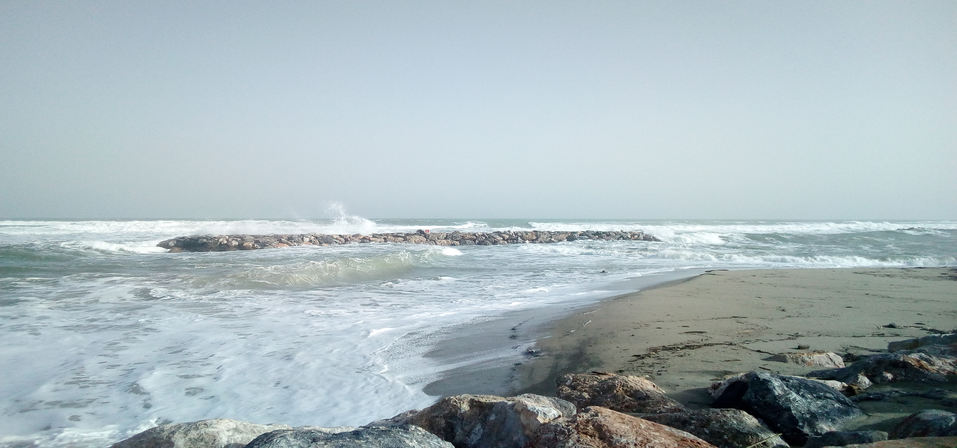
\includegraphics[width=7in]{images/cover_sea}}
    % \newsavebox{\windmill}
    % \savebox{\windmill}{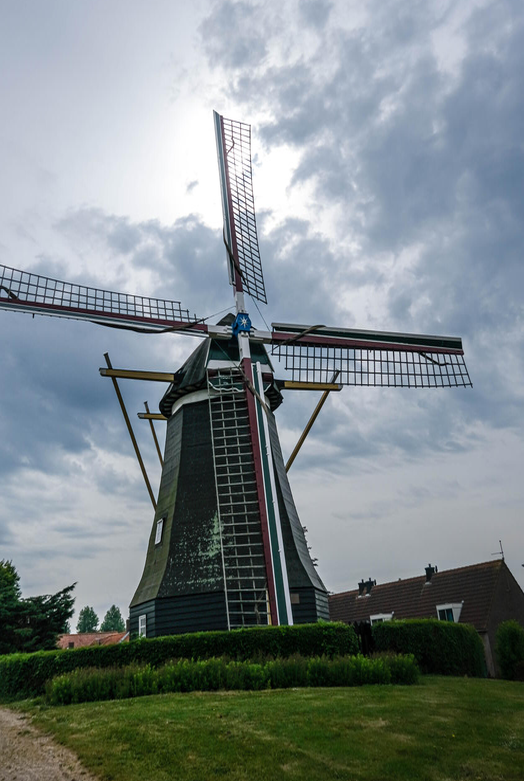
\includegraphics[width=2.5in]{images/cover_windmill}}
    \newsavebox{\bridge}
    \savebox{\bridge}{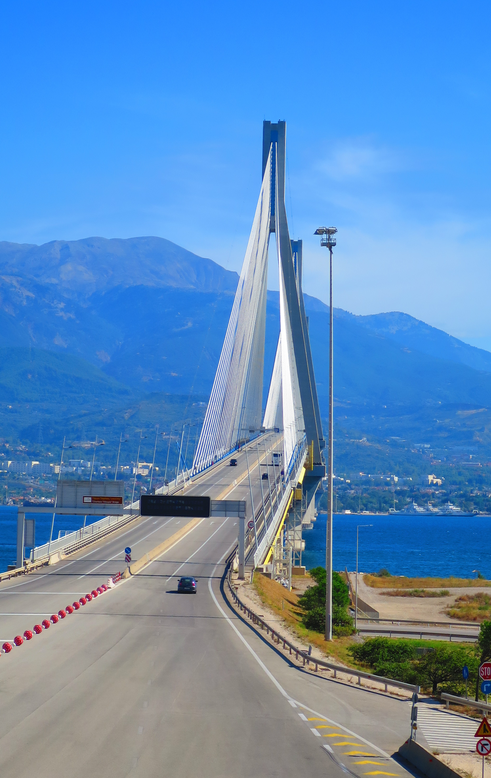
\includegraphics[width=2.5in]{images/cover_bridge}}
    \begin{inctext}[paper=current, target=mytarget]
      \begin{tikzpicture}
        \coordinate (A) at (0,0);
        \coordinate (B) at (8.5in,11in);
        \fill[use as bounding box,color=cyan!7] (A) rectangle (B);
        \coordinate (C) at ([xshift=0.5in,yshift=0.5in]A);
        \coordinate (D) at ([xshift=-0.5in,yshift=-0.5in]B);
        \draw[rounded corners=0.25in,very thick,black] (C) rectangle (D);
        \node[inner sep=0pt,above right] (sea) at (0.75in,2.5in) {\usebox{\caversea}};
        \fill[cyan!7,path fading=south] (0.75in,4.5in) rectangle (7.75in,5.8in);
        % \node[inner sep=0pt,below right] (windmill) at (0.75in,10in) {\usebox{\windmill}};
        \node[inner sep=0pt,below right] (bridge) at (0.75in,10in) {\usebox{\bridge}};
        \fill[cyan!7,path fading=north] (0.75in,6.02in) rectangle (3.3in,6.9in);
        \fill[cyan!7,path fading=west] (2.8in,6in) rectangle (3.26in,10in);
        \node[text width=10cm,align=flush center,font=\Huge\bfseries] at (5.5in,8in) {\UOtitle};
        \node[inner sep=0pt,above right] (UOlogo) at (1in,1in) {\includegraphics[width=\UOlogoCLopt]{\UOlogoCLloc}};
        \node[text width=6cm,above left,font=\large\bfseries] (author) at (7.5in,1in) {\UOauthor \\ \UO};
      \end{tikzpicture}
    \end{inctext}
  \end{titlepage}
  \pagecolor{white}
  \cleardoublepage
}

%%%%%%%%%%%%%%%%%%%%%%%%%%%%%%%%%%%%%%%%%%%%%%%%%%%%%%%%%%%%%%%%%%%%%%
% The open source page
%%%%%%%%%%%%%%%%%%%%%%%%%%%%%%%%%%%%%%%%%%%%%%%%%%%%%%%%%%%%%%%%%%%%%%
\newcommand{\UOopenloc}{images/open_source}     % Location of the logo
\newcommand{\UOopenopt}{2cm}             % Options for includegraphics

\newcommand{\opensource}{
  \thispagestyle{empty}

  \noindent \copyright\ \UOauthor, \UOyear\ (\UO)
  
  \noindent Adapted version from the notes for the courses MAT3380
  and graduate courses in numerical analysis given at the University
  of Ottawa.

  \noindent This document is available on the following sites.\\
  uO Research: \\ % http://hdl.handle.net/10393/44594 \\
  GitHub: % https://github.com/BenoitDionne/Calculus

  \vspace*{1cm}
  
  \noindent \includegraphics[width=\UOopenopt]{\UOopenloc}

  \noindent Unless otherwise stated, this book is made available under
  the terms of the license
  \href{https://creativecommons.org/licenses/by-nc-sa/4.0/deed.en}{Creative
    Commons Attribution - Non Commercial-Share Alike 4.0 International} (CC BY-NC-SA 4.0)

  \vfill

  \noindent Cover Page:\\
  % The windmill, Netherlands, photo by Louise Oegema.\\
  The Rio–Antirio bridge, Greece, photo by Jean Dionne.\\
  The stormy Mediterranean sea, photo by Louise Oegema.

  \cleardoublepage
}

%%%%%%%%%%%%%%%%%%%%%%%%%%%%%%%%%%%%%%%%%%%%%%%%%%%%%%%%%%%%%%%%%%%%%%
% The bibliography
%%%%%%%%%%%%%%%%%%%%%%%%%%%%%%%%%%%%%%%%%%%%%%%%%%%%%%%%%%%%%%%%%%%%%%
\newcommand{\UObibliography}[1]{
  % \setcounter{chapter}{100}
  \addcontentsline{toc}{chapter}{Bibliography}
  \include{#1}
  \cleardoublepage
}

%%%%%%%%%%%%%%%%%%%%%%%%%%%%%%%%%%%%%%%%%%%%%%%%%%%%%%%%%%%%%%%%%%%%%%
% The index
%%%%%%%%%%%%%%%%%%%%%%%%%%%%%%%%%%%%%%%%%%%%%%%%%%%%%%%%%%%%%%%%%%%%%%
\usepackage{makeidx}
\makeindex
\newcommand{\UOindex}{
  \setcounter{chapter}{100}
  \addcontentsline{toc}{chapter}{\indexname}
  \printindex
}

%%%%%%%%%%%%%%%%%%%%%%%%%%%%%%%%%%%%%%%%%%%%%%%%%%%%%%%%%%%%%%%%%%%%%%
% graphics, ...
%%%%%%%%%%%%%%%%%%%%%%%%%%%%%%%%%%%%%%%%%%%%%%%%%%%%%%%%%%%%%%%%%%%%%%
\usepackage{graphicx}
\usepackage{rotating}    % To rotate figures, tables, ...
\usepackage{color}
% \usepackage{tikz}
% \usepackage{pst-node,pst-plot,auto-pst-pdf}
% \usepackage{subfig}

% By default figures will be placed "here" if possible otherwise at
% the "top."
\makeatletter
\renewcommand*{\fps@figure}{ht}
\makeatother

% Methods for jpg, png, ... figures.

\newcommand{\figbox}[2]{\begin{center}%
\includegraphics[width=#2]{#1}\end{center}}

% Methods for pdf figures.
\newcommand{\pdfbox}[1]{\begin{center}\input{#1.pdf_t}\end{center}}

\newcommand{\pdfF}[5][TTT]{%
  \ifthenelse{\equal{TTT}{#1}}{\begin{figure}}{\begin{figure}[#1]}%
      {\color{purple}\rule{\textwidth}{1pt}}\begin{center}%
        \input{#2.pdf_t}\end{center}\caption[#3]{#4 \label{#5}}%
      {\color{purple}\rule{\textwidth}{1pt}}%
    \end{figure}}

\newcommand{\pdfFD}[6][TTT]{
  \ifthenelse{\equal{TTT}{#1}}{\begin{figure}}{\begin{figure}[#1]}%
      {\color{purple}\rule{\textwidth}{1pt}}\begin{center} %
        \input{#2.pdf_t}\end{center} %
      \begin{center}\input{#3.pdf_t}\end{center} %
      \caption[#4]{#5 \label{#6}}%
      {\color{purple}\rule{\textwidth}{1pt}}%
    \end{figure}}

% Methods for png, jpg, ... figures.

\newcommand{\mathF}[6][TTT]{%
  \ifthenelse{\equal{TTT}{#1}}{\begin{figure}}{\begin{figure}[#1]}%
      {\color{purple}\rule{\textwidth}{1pt}}\begin{center} %
        \includegraphics[width=#3]{#2}\end{center} %
      \caption[#4]{#5 \label{#6}}%
      {\color{purple}\rule{\textwidth}{1pt}}%
    \end{figure}}

\newcommand{\mathFD}[7]{\begin{figure}%
    {\color{purple}\rule{\textwidth}{1pt}}\begin{center}%
      \includegraphics[width=#2]{#1}\includegraphics[width=#4]{#3}\end{center}%
    \caption[#5]{#6 \label{#7}}%
    {\color{purple}\rule{\textwidth}{1pt}}\end{figure}}

% Formats for the remarks, examples, ...
\newenvironment{rmk}[1][TTT]%
{\refstepcounter{focus} \noindent %
{\bfseries Remark \arabic{chapter}.\arabic{section}.\arabic{focus}}\ %
\ifthenelse{\equal{TTT}{#1}}{}{({\bfseries #1})}\\ \noindent %
}{\hspace*{\fill} $\spadesuit$}

\newenvironment{rmkList}%   % special case for remarks starting with a list
{\refstepcounter{focus} \noindent %
{\bfseries Remark \arabic{chapter}.\arabic{section}.\arabic{focus}}\\ %
\vspace*{-2\topskip}\noindent}%
{\vspace*{-\topskip}\hspace*{\fill} $\spadesuit$}

\newenvironment{egg}[1][TTT]{%
  \refstepcounter{focus}\noindent%
  {\bfseries Example \arabic{chapter}.\arabic{section}.\arabic{focus}}\ %
  \ifthenelse{\equal{TTT}{#1}}{}{({\bfseries #1})}\\ \noindent %
}{\hspace*{\fill} $\clubsuit$}

\newenvironment{eggList}[1][TTT]{ % special case for ex. starting with a list
  \refstepcounter{focus}\noindent%
  {\bfseries Example \arabic{chapter}.\arabic{section}.\arabic{focus}}\ %
  \ifthenelse{\equal{TTT}{#1}}{}{ ({\bfseries #1})} \\ %
  \vspace*{-2\topskip} \noindent %
}{\vspace*{-\topskip}\hspace*{\fill} $\clubsuit$}

% Title for the multiple choices, the parts of a proof, etc.
\newcommand{\subQ}[1]{\noindent {\bfseries #1})\ }
\newcommand{\subI}[1]{\noindent {\bfseries #1}:\ }
\newcommand{\stage}[1]{\noindent {\bfseries #1}) \ }

%%%%%%%%%%%%%%%%%%%%%%%%%%%%%%%%%%%%%%%%%%%%%%%%%%%%%%%%%%%%%%%%%%%%%%
% Mathematical symbols, short cuts, ...
%%%%%%%%%%%%%%%%%%%%%%%%%%%%%%%%%%%%%%%%%%%%%%%%%%%%%%%%%%%%%%%%%%%%%%
\newcommand{\NN}{\mathbb{N}}
\newcommand{\NNp}{\mathbb{N}^+}
\newcommand{\ZZ}{\mathbb{Z}}
\newcommand{\RR}{\mathbb{R}}
\newcommand{\QQ}{\mathbb{Q}}
\newcommand{\CC}{\mathbb{C}}

\newcommand{\BB}{\mathcal{B}}   % Denotes an atlas for a manifold
\newcommand{\EE}{\mathcal{E}}
\newcommand{\FF}{\mathcal{F}}
\newcommand{\GG}{\mathcal{G}}
\newcommand{\LL}{\mathcal{L}}   % For linear space of bounded operators, ...
\newcommand{\KK}{\mathcal{K}}   % For linear space of compact operators, ...
\renewcommand{\SS}{\mathcal{S}} % For schwartz rapidly decreasing functions, ..
\newcommand{\DD}{\mathcal{D}}   % For the test functions, ...
\newcommand{\DO}{\mathcal{D}}   % For the domain of a function, ...
\newcommand{\B}{\mathcal{B}}
\newcommand{\D}{\mathcal{D}}
\newcommand{\E}{\mathcal{E}}
\newcommand{\F}{\mathcal{F}}
\newcommand{\Q}{\mathcal{Q}}
\newcommand{\U}{\mathcal{U}}
\newcommand{\X}{\mathcal{X}}
\newcommand{\Y}{\mathcal{Y}}
\newcommand{\MM}{\mathcal{M}}
\newcommand{\OO}{\mathcal{O}}
\newcommand{\PP}{\mathcal{P}}
\newcommand{\IMG}{\mathcal{R}}      % For the range of a function, ...
\newcommand{\KE}{\mathcal{N}}       % For the kernel of a function, ...
\newcommand{\GR}{\mathcal{G}}       % For the graph of a function, ...
\newcommand{\HW}{H_{\VEC{w}}}

\DeclareMathOperator*{\esssup}{ess\;sup}
\DeclareMathOperator*{\essinf}{ess\;inf}
\DeclareMathOperator{\arcsec}{arcsec}
\DeclareMathOperator{\tr}{tr}
\DeclareMathOperator{\Id}{Id}
\DeclareMathOperator{\sgn}{sgn}
% \DeclareMathOperator{\diff}{D}
\newcommand{\diff}{\mathrm{D}}
\DeclareMathOperator{\supp}{supp}
\DeclareMathOperator{\curL}{curl}
\DeclareMathOperator{\diV}{div}
\DeclareMathOperator{\graD}{\nabla}
\DeclareMathOperator{\rank}{rank}
\DeclareMathOperator{\RE}{Re}      % For the real part of a number, ...
\DeclareMathOperator{\IM}{Im}      % For the imaginary par of a number, ...
\DeclareMathOperator{\Fix}{Fix}
\DeclareMathOperator{\Per}{Per}
\DeclareMathOperator{\sep}{sep}    % For the section on ``Melnikov
                                   % Function'', file melnikov.tex
\DeclareMathOperator{\Span}{span}
\DeclareMathOperator{\diam}{diam}

\newcommand{\VEC}[1]{\mathbf{#1}}
\newcommand{\ps}[2]{ \left\langle{#1} , {#2}\right\rangle }
\newcommand{\conj}[1]{\overline{#1}}
\newcommand{\HH}{$H_{\VEC{w}}$}
\newcommand{\AP}{AP}
\newcommand{\SN}[1]{\mathrm{S}_{#1}}
\newcommand{\Sone}{S^1}
\newcommand{\torus}[1]{\mathbf{T}^{#1}}
\newcommand{\dist}[2]{\mathrm{dist}\left(#1,#2\right)}
\newcommand{\sgm}[1]{\overline{#1}}
\newcommand{\ii}{\VEC{i}}
\newcommand{\jj}{\VEC{j}}
\newcommand{\kk}{\VEC{k}}
\newcommand{\nn}{$n\times n$\ }
\newcommand{\nm}[2]{${#1}\times{#2}$\ }
\newcommand{\intpt}[1]{\lfloor{#1}\rfloor}

\newcommand{\dx}[1]{\,\mathrm{d}#1}
\newcommand{\dydx}[2]{\frac{\mathrm{d}#1}{\mathrm{d}{#2}}}
\newcommand{\dydxn}[3]{\frac{\mathrm{d}^{#3}{#1}}{\mathrm{d}{#2}^{#3}}}
\newcommand{\dfdx}[2]{\frac{\mathrm{d}}{\mathrm{d}{#2}}{#1}}
\newcommand{\dfdxn}[3]{\frac{\mathrm{d}^{#3}}{\mathrm{d}{#2}^{#3}}{#1}}

\newcommand{\pdydx}[2]{\frac{\partial{#1}}{\partial{#2}}}
\newcommand{\pdydxn}[3]{\frac{\partial^{#3}{#1}}{\partial{#2}^{#3}}}
\newcommand{\pdydxnm}[6]{\frac{\partial^{#4}{#1}}%
{\partial{#2}^{#5} \partial{#3}^{#6}}}
\newcommand{\pdydxdots}[8]{\frac{\partial^{#5}#1}%
{\partial{#2}^{#6} \partial{#3}^{#7} \ldots \partial{#4}^{#8}}}

\newcommand{\pdfdx}[2]{\frac{\partial}{\partial{#2}}{#1}}
\newcommand{\pdfdxn}[3]{\frac{\partial^{#3}}{\partial{#2}^{#3}}{#1}}
\newcommand{\pdfdxnm}[6]{\frac{\partial^{#4}}%
{\partial{#2}^{#5} \partial{#3}^{#6}}{#1}}

\newcommand{\fdiff}[2]{\mathrm{D}^{#2}{#1}}

\newcommand{\dtx}[1]{\Delta{#1}}
\newcommand{\dtxn}[2]{\Delta^{#1}{#2}}

\DeclareMathOperator{\fl}{fl}
\DeclareMathOperator{\Bot}{\,\bot\,}
\newcommand{\tildev}[1]{\tilde{\VEC{#1}}}
\newcommand{\pps}[2]{\left\llangle{#1} , {#2}\right\rrangle }
                                                       % pseudo scalar product

% For the section of Fast Fourier Transform
\newcommand{\fct}[1]{\mathbf{#1}}
\newcommand{\fctt}[1]{\tilde{\mathbf{#1}}}

\newcommand{\NNN}{\mathcal{N}}
\newcommand{\GL}[1]{\mathrm{GL}(#1)}

%%%%%%%%%%%%%%%%%%%%%%%%%%%%%%%%%%%%%%%%%%%%%%%%%%%%%%%%%%%%%%%%%%%%%%
% Trouble
%%%%%%%%%%%%%%%%%%%%%%%%%%%%%%%%%%%%%%%%%%%%%%%%%%%%%%%%%%%%%%%%%%%%%%
\newcommand{\MORE}{\begin{center}\fbox{\color{red}\bfseries TO BE COMPLETED}\end{center}}
\newcommand{\BUG}{\begin{center}\fbox{\color{red}\bfseries TO BE FIXED}\end{center}}


\setSOL

\begin{document}

\pagenumbering{roman}

\titlePage

\opensource

\UOtableofcontents
% \UOfigureslist
% \UOtableslist

\pagenumbering{arabic}

\nonumchapter{Preface}

This book cover the material normally presented in a two-term course on
numerical analysis.  It starts with the basic concept normally presented
in a first course on numerical analysis.  It ends with topics that are
more appropriated for a first course in numerical analysis for
differential equations.

This book can be used by two different groups of students.  If the
focus is on the algorithms and the theory is ignored, then the book
can be used for an introduction to numerical analysis for engineering
and applied science students.  The book can also be used as an
introduction to numerical analysis for students in mathematics, or
students who plan to study more advanced topics in numerical analysis, if
the theory is covered.  We do not think that there is a need to
emphasize the importance of the theory in numerical analysis.  No
serious progress in numerical analysis is possible without it.
Most of the numerical methods presented in this book is accompanied by
a code in MATLAB.

The background for this book is a two-term course in linear algebra,
a course in real analysis (often called advanced calculus to make
the subject less scary), and a course in ordinary differential
equation for the last part of the book.

This book is divided into several parts.

After a brief introduction to the arithmetic on computers, the
{\em first part} on {\bfseries solving equations} is composed of
Chapter~\ref{chaptSeqA} on iterative methods to solve nonlinear
equations of one unknown variable, Chapter~\ref{chaptSeqB} on
iterative methods to solve systems of linear equations,
Chapter~\ref{chaptSeqC} on algebraic methods to solve systems of
linear equations, and Chapter~\ref{chaptSeqD} on iterative methods to
solve system of nonlinear equations.

The {\em second part} of the book on {\bfseries polynomial interpolation}
is composed of Chapter~\ref{chaptInterA} on polynomial interpolation of
real valued functions and Chapter~\ref{chaptInterB} on spline
interpolation; in particular, cubic splines and Bézier curves.

The {\em third part} on the {\bfseries approximation of functions} is
composed of three short chapters: Chapter~\ref{chaptApproxA} on
continuous least square approximation (i.e.\ in $L^2$), 
Chapter~\ref{chaptApproxB} on uniform approximation of real
valued functions and Chapter~\ref{ChaptApproxC} on discrete least square
approximation (i.e.\ in $\ell^2$).

The {\em fourth part} on finding {\bfseries eigenvalues} of matrices
is composed of only one chapter, Chapter~\ref{chapEigVal}, on
numerical methods to compute eigenvalues of \nn matrices.

The {\em last part} on {\bfseries differential equations} is
composed of Chapter~\ref{chaptDiffInt} on the numerical
differentiation and integration of real valued functions,
Chapter~\ref{chaptInitVal} on the numerical methods to solve initial
value problems for ordinary differential equations,
Chapter~\ref{chapBoundValProbl} on the numerical methods to solve
boundary value problems for ordinary differential equations, and
Chapter~\ref{FiniteDiffMeth} on finite difference methods to solve
partial differential equations.

There is no chapter on finite element methods to solve partial
differential equations.  This topic requires some knowledge of
functional analysis to be properly covered.  To keep the book
accessible the undergraduate students (as much as possible), no
knowledge of functional analysis is assumed. 

The second and third part of the book are related and even
intertwine in some cases.  There are many ways to approximate a
function $f:[a,b] \rightarrow \RR$ by polynomials.  The major
approaches are:

\begin{enumerate}
\item Given any small $\epsilon$, we could find a polynomial
$p_\epsilon$ such that
\[
\max_{a\leq x \leq b} \,|f(x) - p_\epsilon(x)| < \epsilon \ .
\]
Stone-Weierstrass Theorem, Theorem~\ref{SWtheorem}, states that
$p_\epsilon$ can always be found if $f$ is a continuous function on
$[a,b]$.  The function $f$ is
{\bfseries uniformly approximate}\index{Functions!Uniformly Approximate}
by the polynomial $p_\epsilon$.  This will
be studied in Chapter~\ref{chaptApproxB}.  This very short
chapter is more theoretical.  Nevertheless, it is important to
understand the limitations of polynomial interpolation and splines
presented in Chapters~\ref{chaptInterA} and
\ref{chaptInterB}.
\item Given any small $\epsilon$, we could find a polynomial
$p_\epsilon$ such that
\[
\int_a^b \,|f(x) - p_\epsilon(x)|^2 \dx{x} < \epsilon \ .
\]
The polynomial $p_\epsilon$ is a
{\bfseries quadratic approximation}\index{Functions!Quadratic Approximation}
of the function $f$.  This will be studied in Chapter~\ref{chaptApproxB}.
Again, this chapter is more theoretical but essential to understand
discrete least square approximation in Chapter~\ref{ChaptApproxC}.
This material is also fundamental in the study of numerical analysis;
in particular, to develop methods to solve partial differential
equations.
\item Given any small $\epsilon$ and
$a \leq x_0 < x_1 < x_2 < \ldots < x_n \leq b$, we could find a polynomial
$p_\epsilon$ such that
\[
\sum_{i=0}^n \,|f(x_i) - p_\epsilon(x_i)|^2 < \epsilon \ .
\]
This is a {\bfseries discrete least square
approximation}\index{Functions!Discrete Least Square Approximation}
of the data set
\[
\{(x_i,f(x_i)) : i=0,1,2,\ldots, n\}
\]
by a polynomial.  This will be the subject of Chapter~\ref{ChaptApproxC}.
\item We could also find a polynomial $p$ of degree at most
$n$ such that $p(x_i) = f(x_i)$ for $0 \leq i \leq n$.  This is the
subject of Chapter~\ref{chaptInterA}.
\item Instead of looking for a polynomial of degree $n$, where $n$ may
be large, we could find polynomials $p_i$ of small degrees (usually of
degree $3$) such that $p_i$ is an approximation of $f$ on the small
interval $[x_i,x_{i+1}]$.  The polynomials $p_i$ are determined from
conditions at the endpoints $x_i$ that provide some degree of
smoothness for the piecewise polynomial $p$ defined by $p(x) = p_i(x)$
for $x\in [x_i, x_{i+1}]$.  The polynomial $p$ is called a
{\bfseries spline}\index{Spline}.   We will present the
{\bfseries cubic splines}\index{Functions!Cubic Spline
Interpolation}, {\bfseries B\'ezier curves}\index{B\'ezier Curves} and
{\bfseries B-Splines}\index{Functions!B-Spline Interpolation}
in Sections~\ref{CSI}, \ref{BEZIER} and \ref{BSI} of
Chapter~\ref{chaptInterB}.  These piecewise polynomial approximations
are superior to the simple polynomial interpolation mentioned in the
previous item.  Cubic splines, B\'ezier curves, ... are used in some
of the major software for drawing.
\end{enumerate}

There is a strong emphasis in this book on differential equations.
This is only a reflect of the principal interest of the author.
Contrary to must introductory textbooks in numerical analysis, 
there is an extensive chapter, Chapter~\ref{chaptInitVal}, on the
numerical methods to solve initial value problems for ordinary
differential equations.  There is also a full chapter,
Chapter~\ref{chapBoundValProbl}, on the numerical methods to solve
boundary value problems for ordinary differential equations, and 
a full chapter, Chapter~\ref{FiniteDiffMeth}, on finite difference
methods.

There are many solved exercises at the end of several chapters.  Most
of the exercises are to reinforce the concepts presented in the text.
We have kept the number of theoretical questions to the minimum.
This was mainly motivated by the groups of students who took the
numerical analysis courses.  They were more interested in the
applications of numerical analysis than in the theory.  Sadly, there
are not real life applications of numerical analysis in this book.  It
would be nice (in the future) to add some realistic projects to
illustrate each topics.

The examples should be treated as problems to be solved by the reader.
The reader should try to answer each problem before looking at its
solution (if it is available).

In this book, we use the following notation for some standard
sets of numbers.

\begin{defn*}
The following well known sets are frequently used in this document.
\begin{itemize}
\item $\NN = \{0,1,2,3,\ldots \}$ is the set of natural numbers.
\item $\NNp = \{1,2,3,\ldots \}$ is the set of positive natural numbers.
\item $\ZZ = \{0,1,-1,2,-2,3,-3, \ldots \}$ is the set of integers.
\item $\QQ$ is the set of rational numbers.
\item $\RR$ is the set of real numbers.
\item $\CC$ is the set of complex numbers.
\end{itemize}
\end{defn*}

We will also often use the following definition when approximating
functions.

\begin{defn*} Let $f:\RR^n \rightarrow \RR$ and
$g:\RR^n \rightarrow \RR$ be two functions.  We write
$f\left(\VEC{x}\right) = O\left(g\left(\VEC{x}\right)\right)$ near
the origin if there exists a positive constant $K$ such that
\[
\left| f\left(\VEC{x}\right) \right| < K \left| g\left(\VEC{x}\right) \right|
\]
for $\VEC{x}$ in a neighbourhood of the origin.  We write
$f\left(\VEC{x}\right) = o\left(g\left(\VEC{x}\right)\right)$ near
the origin if
\[
\lim_{\VEC{x}\rightarrow \VEC{0}} \frac{f\left(\VEC{x}\right)}
{g\left(\VEC{x}\right)} = 0 \ .
\]
\end{defn*}

%%% Local Variables: 
%%% mode: latex
%%% TeX-master: "notes"
%%% End: 

\cleardoublepage

\chapter{Computer Arithmetic}\label{chaptArith}

Before studying algorithms to perform computations with computers, we
need to understand how computers perform basic arithmetic operations.
It is the goal of this chapter.

\section{Rounding}

\begin{defn}
The {\bfseries normalized scientific notation}\index{Normalized
Scientific Notation} for a real number is
$\pm 0.d_1d_2d_3\ldots \times 10^m$, where $m$ is an
integer, $d_i \in \{0,1,2,3,\ldots,9\}$ and $d_1 \neq 0$.
\end{defn}

Before performing any arithmetic operation with real numbers, we will
always assume that they have been expressed in the normalized
scientific notation.

When performing arithmetic operations by hand, we often have to
consider only the first few decimals (digits after the period) of the
numbers used in the operations and ignore the others.  This is called
{\bfseries rounding}\index{Rounding}.

There are different ways to perform rounding.  We will mention only
two.

\begin{defn}
Let $\pm 0.d_1 d_2 \dots \times 10^N$ be the normalized scientific
representation of a real number $a$, thus $d_1 \neq 0$.  For $k$ a
positive integer, we define the\\
{\bfseries k-digit chopping representation}\index{k-digit Chopping
  Representation} of $a$ to be
$\pm 0.d_1 d_2 \dots d_k \times 10^N$, and the\\
{\bfseries k-digit rounding representation}\index{k-digit Rounding
  Representation} of $a$ to be
$\pm 0.d_1 d_2 \dots d_k \times 10^N + \epsilon \; 10^{-k} \times 10^N$,
where $\epsilon = 1$ for $d_{k+1}\geq 5$ and $\epsilon = 0$ for
$d_{k+1} < 5$.
\end{defn}

If $\tilde{a}$ is the k-digit chopping representation of $a$, then
$|a-\tilde{a}| < 10^{-k}\times 10^N$.  If $\tilde{a}$ is 
k-digit rounding representation of $a$, then
$|a-\tilde{a}| \leq 0.5 \times 10^{-k}\times 10^N$.

\begin{egg}
Here are some examples of $3$-digit rounding representations.
\[
\begin{array}{l|@{\hspace{1em}}l}
\text{exact value} & \text{$3$-digit rounding}\\
 & \text{approximation}\\
\hline
0.19234542 \times 10^6 & 0.192 \times 10^6 \\
0.25952100 \times 10^{-5} & 0.260 \times 10^{-5} \\
0.99950000 \times 10^2 & 0.100 \times 10^3
\end{array}
\]
\end{egg}

\begin{egg}
If $0.481\times 10$ is a $3$-digit rounding approximation of $x$ and
$0.12752 \times 10^2$ is a $5$-digit rounding approximation of $y$, find
the interval that will contain the exact value of $x-y$.

Since $4.805 \leq x <4.815$ and $12.7515 \leq y < 12.7525$, then
$4.805-12.7525 <x-y < 4.815-12.7515$.  Thus $-7.9475 < x-y < -7.9365$.
\end{egg}

\section{Binary Number}

Computers only manipulate binary numbers (i.e.\ numbers in base $2$),

Recall that a number in base $2$ is a number of the form
\[
(b_k b_{k-1} \ldots b_1 b_0. b_{-1} b_{-2} \ldots )_2
= b_k 2^k + b_{k-1} 2^{k-1} + \ldots + b_1 2 + b_0 + b_{-1} 2^{-1}
+ b_{-2} 2^{-2} + \ldots
\]
where $b_i \in \{0,1\}$ for all $i$.

\begin{defn}
The {\bfseries normalized binary numbers}\index{Normalized Binary Numbers}
are numbers of the form
$\pm(0.b_1 b_2 b_3 \ldots )_2 \times 2^m$, where $b_i \in \{0,1\}$,
$b_1 = 1$ and $m$ is an integer often represented in binary form. 
Binary numbers in normalized binary form are also said to be in
{\bfseries normalized floating point form}\index{Normalized Floating
Point Form}.
\end{defn}

To find the binary representation of a positive number $x$ in base
$10$, one begins by writing $x$ as $x=m+d$, where $m$ is an integer
and $d<1$.

If
\begin{align*}
m &= m_j\times 10^j + m_{j-1}\times 10^{j-1} + \ldots + m_1 \times 10 +
m_0 \; ,
\intertext{then}
(m)_2 &= (m_j)_2 \times (10)_2^j + (m_{j-1})_2\times (10)_2^{j-1} +
\ldots + (m_1)_2 \times (10)_2 + (m_0)_2 \; .
\end{align*}
The easiest way to evaluate this expression is recursively.
\begin{align*}
\alpha_0 &= (m_j)_2 \\
\alpha_1 &= \alpha_0 \times (10)_2+(m_{j-1})_2 \\
\alpha_2 &= \alpha_1 \times (10)_2+(m_{j-2})_2 \\
\vdots & \qquad \vdots \\
\alpha_{j-2} &= \alpha_{j-3} \times(10)_2 + (m_2)_2 \\
\alpha_{j-1} &= \alpha_{j-2} \times(10)_2 + (m_1)_2 \\
\alpha_j &= \alpha_{j-1} \times(10)_2 + (m_0)_2
\end{align*}
and $(m)_2 = \alpha_j$.

Let
\[
  d = d_1 \times 2^{-1} + d_2 \times 2^{-2} + d_3 \times 2^{-3} +
  \ldots + d_k \times 2^{-k} \ .
\]
The first digit $d_1$ is the integer part of
\begin{align*}
r_1 &= 2 d = 2 \times \left(d_1 \times 2^{-1} + d_2\times 2^{-2} +
\ldots + d_{1-k} \times 2^{1-k} + d_k\times 2^{-k} \right) \\
&= d_1 + d_2\times 2^{-1} +
\ldots + d_{k-1} \times 2^{2-k} + d_k\times 2^{1-k} \ .
\end{align*}
The second digit $d_2$ is the integer part of
\begin{align}
r_2 &= 2^2 (d - d_1\times 2^{-1})
= 2^2 \times \left(d_2 \times 2^{-2} + d_3\times 2^{-3} +
\ldots + d_{k-1} \times 2^{1-k} + d_k\times 2^{-k} \right) \nonumber \\
&= d_2 + d_3\times 2^{-1} +
\ldots + d_{k-1} \times 2^{3-k} + d_k\times 2^{2-k} \ . \label{C1L1}
\end{align}
The third digit $d_3$ is the integer part of
\begin{align}
r_3 &= 2^3 (d - d_1\times 2^{-1} - d_2 \times 2^{-2}) \nonumber \\
&= 2^3 \times \left(d_3 \times 2^{-3} + d_4\times 2^{-4} +
\ldots + d_{k-1} \times 2^{1-k} + d_k\times 2^{-k} \right) \nonumber \\
&= d_3 + d_4\times 2^{-1} +
\ldots + d_{k-1} \times 2^{4-k} + d_k\times 2^{3-k} \ . \label{C1L2}
\end{align}
In general, we get that the $i^{th}$ digit $d_i$ is the integer part
of
\begin{equation} \label{C1L3}
r_ i = 2^i \left(d - d_1\times 2^{-1} - d_2 \times 2^{-2} - \ldots -
d_{i-1} \times 2^{1-i} \right)
\end{equation}
for $i=2$, $3$, $4$, \ldots. $k$.

We however need a more efficient way to find the digits $d_i$.  We
have from (\ref{C1L1}) that
\begin{equation} \label{C1L4}
  r_2 = 2 (2d - d_1) = 2(r_1 - d_1)\ .
\end{equation}
We have from (\ref{C1L2}) that
\[
r_3 = 2 (\, 2 (2 d - d_1) - d_2 ) = 2 ( r_2 - d_2) \  .
\]

We prove by induction that
\begin{equation} \label{C1L5}
  r_{i+1} = 2 (r_i - d_i )
\end{equation}
for $i=1$, $2$, \ldots, $k-1$.  It follows from (\ref{C1L4}) that
(\ref{C1L5}) is true for $i=1$.  Let's suppose that
(\ref{C1L5}) is true for $i=j<k-1$.  We have from (\ref{C1L3})
with $i=j+2$ that
\begin{align*}
r_{j+2} &= 2^{j+2}\left( d - d_1 2^{-1} - d_2 2^{-2} - \ldots
- d_j 2^{-j} - d_{j+1} 2^{-j-1}\right) \\
&= 2 \bigg( \underbrace{ 2^{j-1} \left( d - d_1 2^{-1} - d_2 2^{-2} - \ldots
d_j 2^{-j}\right)}_{=r_{j+1}\text{ from (\ref{C1L3}) with } i=j+1}
  + d_{j+1} \bigg) \\
&= 2 \left( r_{j+1} - d_{j+1}\right) \ .
\end{align*}
This is (\ref{C1L5}) with $i=j+1$.  This complete the proof by
induction.

\begin{egg}
The binary representation of $1/10$ is $(0.0\overline{0011})_2$.

Let $(1/10)_2 = (0.d_1 d_2 d_3 \ldots)_2$.  We summarize in the
table below the computation using $r_1 = 2 d$ and
$r_{i+1} = 2 (r_i - d_i )$ for $i=1$, $2$, \ldots
\[
\begin{array}{l|l|l}
\hline
i & r_ i & d_i \\
 & & \text{(the integer part of $r_i$)} \\
\hline
1 & 2 \times 1/10 = 1/5 & 0 \\
2 & 2 (r_1 - 0) = 2/5 & 0 \\
3 & 2 (r_2 - 0) = 4/5 & 0 \\
4 & 2 (r_3 - 0) = 8/5 = 1.6 & 1 \\
5 & 2 (r_4 - 1) = 6/5 = 1.2 & 1 \\
6 & 2 (r_5 - 1) = 2/5 & 0 \\
\vdots & \qquad \vdots & \vdots \\
\hline
\end{array}
\]
Since $r_6 = r_2$ and $d_6 = d_2$, we get that $d_7 = d_3$,
$d_8=d_4$, $d_9 = d_5$ and, in general, $d_i= d_{i-4}$ for $i=6$, $7$,
\ldots.
\end{egg}

\section{Computer Numbers}

To illustrate the properties of computer arithmetic, we assume that
each real number is stored in a 32-bit word.  The typical computer
representation of a normalized binary number
$x = \pm(0.b_1 b_2 b_3 \ldots )_2 \times 2^m$ is given by
\[
\begin{array}{|c|c|c|}
\hline
s & e_8 e_7 e_6 \ldots e_1 & b_2 b_3 \ldots b_{24} \\
\hline
\end{array} \ ,
\]
where $s$ indicates the sign of $x$,
$(e_8 e_7 \ldots e_1)_2 = (m)_2 + (1111111)_2$, and
$b_1$, $b_2$, $b_3$, \ldots $b_{24}$ are the
first $24$ binary digits of the normalized representation of $x$.
The part $(b_1 b_3 \ldots b_{24})_2$ is called the
{\bfseries normalized mantissa}\index{Normalized Mantissa}.

\begin{rmkList}
\begin{enumerate}
\item We did not store the value of $b_1$ because we always assume
that the binary numbers are normalized and so $b_1$ is always $1$.
\item Let $e$ be the decimal representation of the number
$(e_8 e_7 \ldots e_1)_2$.  Then $0 \leq e < 2^8 = 256$ but, in
practice, only $1 \leq e \leq 254$ is used because the values $0$ and
$255$ are often reserved to indicate really small or large numbers,
and {\bfseries NaN}\index{NaN} (not a number).  We get NaN following an illegal
operation like a division by zero.

To represent negative exponents, we assume that $e = m + 127$.  Thus,
$-126 \leq m \leq 127$.  In binary notation
$(m)_2 = (e_8 e_7 \ldots e_1)_2 - (1111111)_2$.
\item $0$ has its unique computer representation (associated to $e=0$
or $255$).
\end{enumerate}
\end{rmkList}

The computer representation of a real number $x$ is called the
{\bfseries floating point representation}\index{Floating Point
  Representation} of $x$ and is denoted by
$\fl(x)$.  The difference between a real number and its computer
representation is called the {\bfseries rounding error}\index{Rounding Error}.

There are major differences between the standard arithmetic and the
computer arithmetic.  We mention some below.

\begin{itemize}
\item Not all real numbers can be represented as computer numbers.
There are ``holes'' in the computer representation of the real line.
For instance, the binary representation of $1/10$ is
$(0.\overline{1100})_2 \times 2^{-(11)_2}$.  Hence, the machine
representation of this number is
\[
\begin{array}{|c|c|c|}
\hline
0 & 1111100 & 10011001100110011001100 \\
\hline
\end{array} \ .
\]
This machine number represents in fact the number
\begin{align*}
&\big( 2^{-1} + 2^{-2} + 2^{-5} + 2^{-6} + 2^{-9} + 2^{-10} +
2^{-13} + 2^{-14} + 2^{-17} + 2^{-18} \\
&\qquad + 2^{-21} + 2^{-22}\big) 2^{-3} = 0.09999999403954\ldots
\end{align*}
\item Not all real numbers can be represented as computer numbers.
There are upper and lower bounds to the real numbers that can be
represented on a computer. The largest real number that can be
represented as computer number is
\[
R_M =(0.\underbrace{1111\ldots1}_{\text{24 times}})_2 \times 2^{127} =
( 1 - 2^{-24})\times 2^{127} \approx 0.17014117\ldots \times 10^{38}
\]
and the smallest positive number is
\[
R_m =(0.1\underbrace{000\ldots0}_{\text{23 times}})_2 \times 2^{-126}
= 2^{-127} \approx 0.587747\ldots \times 10^{-38}  \ .
\]
If the result of a computation is a number bigger than $R_M$, then we
say that we have {\bfseries overflow}\index{Overflow}.  If the result
of a computation is a number smaller than $R_m$, than we have
{\bfseries underflow}\index{Underflow}.

\item The fundamental algebraic properties of the real number system
(commutativity, associativity, \ldots) are not preserved. 

Suppose that the basic computer operations ($+$, $-$, $\times$,
$\div$) are defined as follows. 
\[
\begin{array}{l|l}
\text{exact operation} & \text{computer operation} \\
\hline
x \pm y & \fl(\fl(x) \pm \fl(y)) \\
x \times y & \fl(\fl(x) \times \fl(y))\\
x \div y & \fl(\fl(x) \div \fl(y))
\end{array}
\]
We also define the computer operation $\fl(\sqrt{\fl(x)})$ to
represent the exact operation $\sqrt{x}$.  This is not exactly how
computers work with computer numbers but it is an acceptable
definition to understand why the fundamental algebraic
properties of the real number system are not preserved.

If we work in base $10$ using $4$-digit rounding representations, the
computer evaluation of $\pi + (1/3) \times \pi$ is given by
\begin{align*}
\fl(\fl(\pi)+\fl(\fl(1/3) \times \fl(\pi)))
&= \fl( (0.3142\times 10) + \fl( 0.3333 \times (0.3142 \times 10) )) \\
&= \fl( (0.3142\times 10) + \fl( 1.0472286000000  )) \\
&= \fl( (0.3142\times 10) + (0.1047 \times 10) ) \\
&= \fl( 4.189 ) = 0.4189 \times 10
\end{align*}
The computer evaluation of
$\pi \times (1 + (1/3))= \pi + (1/3)\times \pi$ is given by 
\begin{align*}
\fl( \fl(\pi) \times \fl( \fl(1) + \fl(1/3)))
&= \fl( (0.3142\times 10) \times \fl( (0.1\times 10) + (0.3333) )) \\
&= \fl( (0.3142\times 10) \times \fl(1.3333) ) \\
&= \fl( (0.3142\times 10) \times (0.1333\times 10) ) \\
&= \fl( 4.188286 ) = 0.4188 \times 10
\end{align*}
Thus, we do not get the same $4$-digit rounding representation for
$\pi + (1/3)\times \pi$ and $\pi \times (1 + (1/3))$.  The
distributive law is not preserved.
\end{itemize}

Suppose that $p$ is the exact result of a computation and $\tilde{p}$
is the computer result of this computation.  The number
$\epsilon = |p-\tilde{p}|$ is the
{\bfseries absolute error}\index{Absolute Error}.
If $p\neq 0$, the number
$\epsilon_r= |p-\tilde{p}|/|p|= \epsilon/|p|$
is the {\bfseries relative error}\index{Relative Error}.

If the absolute error is $0.1$, where the numbers $p$ and $\tilde{p}$
are smaller than $1$ in absolute value, then the error is enormous.
However, when the numbers $p$ and $\tilde{p}$ are larger than $10^6$
in absolute value, the same absolute error is very small.  The
absolute error by itself does not say anything about the accuracy of
the computation.  The relative error is the useful information about
the size of the error.

\begin{egg}
$22/7$ and $315/113$ are two frequently used approximations of $\pi$.
We find the absolute and relative errors of these two approximations
of $\pi$.  The absolute and relative error of the approximation $22/7$ of
$\pi = 3.14159265358979\ldots$ are
\[
|3.14159265358979\ldots- 22/7| = 0.126442\ldots \times 10^{-2}
\]
and
\[
|3.14159265358979\ldots
- 22/7|/3.14159265358979\ldots = 0.4024994\ldots\times 10^{-3}
\]
respectively.  A relative error of about $0.04$ \%.  The absolute and
relative error of the approximation $355/113$ of $\pi$ are
\[
|3.14159265358979\ldots- 355/113| =
0.2668\ldots\times 10^{-6}
\]
and
\[
|3.14159265358979\ldots - 355/113|/3.14159265358979\ldots
= 0.84914\ldots\times10^{-7}
\]
respectively.  A relative error of about $0.0000085$ \%.
\end{egg}

\begin{rmk}
For our 32-bit computer, if $x=(0.b_1 b_2 b_3\ldots)_2 \times 2^m$, we 
have that $\displaystyle \frac{|x-\fl(x)|}{|x|} \leq 2^{-24}$ if rounding
is used and $\displaystyle \frac{|x-\fl(x)|}{|x|} \leq 2^{-23}$ if
chopping is used.

\stage{i} We prove that $\displaystyle \frac{|x-\fl(x)|}{|x|}
\leq 2^{-24}$ if rounding is used.  The number $x$ is between the
computer numbers $x_1 = (0.b_1b_2b_3\ldots b_{24})_2 \times 2^m$ and
$x_2 = ((0.b_1b_2b_3\ldots b_{24})_2 + 2^{-24}) \times 2^m$.
Hence $\fl(x) = x_1$ if $b_{25} =0$ and $\fl(x) = x_2$ if $b_{25}=1$.

If $b_{25}=0$, then
\[
|x-\fl(x)| = | x- x_1 | = (0.b_{26} b_{27} \ldots)_2 \times 2^{m-25}
\leq 2^{m-25}
\]
and
\[
\frac{|x-\fl(x)|}{|x|} \leq
\frac{2^{m-25}}{(0.b_1 b_2 b_3\ldots)_2 \times 2^m}
= \frac{1}{(0.b_1 b_2 b_3\ldots)_2} 2^{-25} \leq 2^{-24}
\]
because $(0.b_1 b_2 b_3\ldots)_2 \geq (0.b_1)_2 = (0.1)_2 = 2^{-1}$.

If $b_{25}=1$, then
\[
|x-\fl(x)| = | x- x_2 | = ((1)_2 - (0.b_{25} b_{26} \ldots)_2) \times 2^{m-24}
\leq 2^{m-25}
\]
because $(1)_2-(0.b_{25}b_{26} \ldots)_2 \leq 2^{-1}$.  Thus
\[
\frac{|x-\fl(x)|}{|x|} \leq
\frac{2^{m-25}}{(0.b_1 b_2 b_3\ldots)_2 \times 2^m}
= \frac{1}{(0.b_1 b_2 b_3\ldots)_2} 2^{-25}
< 2^{-24}
\]
because $(0.b_1b_2b_3\ldots)_2 \geq (0.b_1)_2 =
(0.1)_2 = 2^{-1}$.

\stage{ii} To prove that
$\displaystyle \frac{|x-\fl(x)|}{|x|} \leq 2^{-23}$ if
chopping is used.  We note that
\[
\fl(x) = (0.b_1b_2b_3\ldots b_{24})_2 \times 2^m
\]
and
\[
|x-\fl(x)| =  (0.b_{25}b_{26} b_{27} \ldots)_2 \times 2^{m-24}
< 2^{m-24} \ .
\]
We do not exclude the possibility that some or all of $b_{25}$,
$b_{26}$, \ldots\ be zero. Thus
\[
\frac{|x-\fl(x)|}{|x|} \leq
\frac{2^{m-24}}{(0.b_1 b_2 b_3\ldots)_2 \times 2^m}
= \frac{1}{(0.b_1 b_2 b_3\ldots)_2} 2^{-24}
< 2^{-23}
\]
because $(0.b_1b_2b_3\ldots)_2 \geq (0.b_1)_1 = (0.1)_2 = 2^{-1}$.
\end{rmk}

\begin{defn}
Let $r$ be a positive integer.  We say that $\tilde{p}$
approximates $p$ to $r$
{\bfseries significant digits}\index{Significant Digits} if
\[
|p - \tilde{p}| \leq \frac{1}{2} \beta^{s-r+1} \ ,
\]
where $\beta$ is the basis used to represent the numbers and $s$
is the largest integer such that $\beta^s \leq |p|$.
\end{defn}

For instance, if the basis is $\beta = 10$, then $\tilde{p}$
approximate $p$ to $r$ significant digits if
\[
|p - \tilde{p}| \leq \frac{1}{2} \left( 10^{s-r+1} \right) = 5 \times 10^{s-r}
\ ,
\]
where $s$ is the largest integer such that $10^s \leq |p|$.  Thus
\[
\frac{|p - \tilde{p}|}{|p|} \leq \frac{|p - \tilde{p}|}{10^s}
\leq 5 \times 10^{-r} \ .
\]
The largest positive integer $r$ such that the previous inequality is
satisfied is the classical definition of $r$ significant digits. 

\begin{egg}
Both $10.001$ and $9.999$ approximate $10$ to $4$ significant
digits because the relative error
\[
\epsilon_r = \frac{|10.001 - 10|}{10} = \frac{|10-9.999|}{10}
= 10^{-4} < 5 \times 10^{-4}
\]
and $4$ is the largest integer $r$ such that $\epsilon_r < 5 \times
10^{-r}$.
\end{egg}

\section{Controlling Errors}

From now on and until the end of this chapter, our presentation will
be more intuitive.  We will not always be mathematically rigorous.
Our goal is to help the readers develop their intuition on how to
improve the accuracy of numerical computations.  This is often
referred as the Art of numerical computation.

There are many causes for the loss of accuracy in computations.

\begin{enumerate}
\item Loss of accuracy often comes from the cancellation of significant
digits due to subtraction of nearly equal numbers.

Let $x= 5/7 = 0.\overline{714285}$ and $y=0.714251$.  Using $5$-digit
chopping arithmetic, we get
\[
\begin{array}{l|c|c|c|c|c}
& \text{Exact} & \text{$5$-digit} & \text{absolute} & \text{relative} &
\text{number of} \\
& \text{values} & \text{chopping} & \text{error} & \text{error} &
\text{significant} \\
& & \text{arithmetic} & \text{(approx.)} & \text{(approx.)} & \text{digits} \\
\hline
x & \rule{0em}{1em} 0.\overline{714285} & 0.71428 & 0.6 \times 10^{-5} &
0.8 \times 10^{-5} & 5 \\
y & 0.714251 & 0.71425 & 0.1 \times 10^{-5} & 0.14\times 10^{-5} & 6 \\
x-y & 0.34\overline{714285}\times 10^{-4} & 0.3 \times 10^{-4} &
0.47\times 10^{-5} & 0.136 & 1
\end{array}
\]
We have lost a lot of significant digits in the subtraction $x-y$.
\item The rounding error of a computer number is amplified when this number
is multiply by a number of large absolute value or divide by a number of
small absolute value.
\item A really small number should not be added to a very large number.
Let $x= 0.1234 \times 10^5$ and $y=0.4321$.  Using $4$-digit rounding
arithmetic to add this two numbers, we get $x+y=x$ because
$y=0.000004321$ and so $x+y$ is $0.123404321 \times 10^5$.  Rounding
this number to $4$-digits gives $x = 0.1234 \times 10^5$.
\end{enumerate}

When possible, rearranging the order of the arithmetic operations may
increase the accuracy of the computation.  The following three examples
illustrate this technique.

\begin{egg}
Use $6$-digit rounding arithmetic to compute the roots of the
polynomial $x^2-20\,x+1=0$.

The standard formulae to compute the
roots of the polynomial of degree two $a x^2+b x+c=0$ are
\begin{equation}
x_{+} =\frac{-b+\sqrt{b^2-4\,a\,c}}{2\,a}
\quad \text{and} \quad
x_{-} =\frac{-b-\sqrt{b^2-4\,a\,c}}{2\,a}  \ . \label{C1L6}
\end{equation}
We get
\[
x_{+}=\frac{20+\sqrt{396}}{2} \approx \frac{20+19.8997}{2}
\approx 19.9499 \; .
\]
Since the exact value of this root is
$\alpha = 19.9498743710661995\ldots$, the relative error is
\[
\frac{19.9499 - \alpha}{\alpha} \approx 0.128 \times 10^{-5} \ .
\]
The second root is
\[
x_{-}=\frac{20-\sqrt{396}}{2} \approx
\frac{20-19.8997}{2} = \frac{0.1003}{2} = 0.05015 \ .
\]
Since the exact value of this root is $\beta =
0.050125628933800\ldots$, the relative error is
\[
\frac{0.05015 - \beta}{\beta} =\approx 0.486 \times 10^{-3} \ .
\]
This is not really good for $6$-digit rounding.

If $c\neq 0$, the roots of the polynomial $a x^2+b x+c=0$ are also
given by the formulae
\begin{equation}
x_{+} = \frac{-2c}{b+\sqrt{b^2-4\,a\,c}} \quad \text{and} \quad
x_{-} = \frac{2c}{-b+\sqrt{b^2-4\,a\,c}} \ .  \label{C1L7}
\end{equation}
Multiply the formula for $x_{+}$ in (\ref{C1L6}) by
$\displaystyle \frac{-b-\sqrt{b^2-4ac}}{-b-\sqrt{b^2-4ac}}$ and the
formula for $x_{-}$ in (\ref{C1L6}) by
$\displaystyle \frac{-b+\sqrt{b^2-4ac}}{-b+\sqrt{b^2-4ac}}$ to get the
formulae in (\ref{C1L7}).

We get
\[
x_{-} = \frac{2}{20+\sqrt{396}} \approx \frac{2}{20+19.8997}
= \frac{2}{39.8997} \approx 0.0501257 \ .
\]
The relative error is now
\[
\frac{0.0501257 - \beta}{\beta} = 0.142 \times 10^{-5} \ .
\]
This is good.  This is a significant improvement on the previous
computation of $x_{-}$.

The idea is to avoid the subtraction of almost equal numbers.  In
the formula for $x_{-}$ in (\ref{C1L6}), we had to
compute $20-19.8997$ which is the difference of two very close numbers.
In the formula for $x_{-}$ in (\ref{C1L7}), we did not have to
subtract two very close numbers.  This is the reason why, for the polynomial
$x^2-20\,x+1=0$, the second formula to compute $x_-$ is better than
the first one.
\end{egg}

\begin{egg}
Compute
\begin{equation} \label{C1L8}
f(x) = x^3 -6x^2+3x-0.149
\end{equation}
at $x=4.71$ using $3$-digit rounding arithmetic.

A direct computation using (\ref{C1L8}) and $3$-digit rounding
arithmetic gives $f(x) = -0.140 \times 10^2$.  Using the fact that
$f(x) = -14.636489$, we find that the absolute error is
$0.636489$, the relative error is about $0.04$, and the
approximation is to $2$ significant digits. 

A better way to write $f(x)$ is to use the nested form
\begin{equation} \label{C1L9}
f(x) = -0.149 +x(3 + x(x-6)) \ .
\end{equation}
Using (\ref{C1L9}) and $3$-digit rounding arithmetic, we get
$f(x) = -0.146 \times 10^2$.  The absolute error is
$0.36489 \times 10^{-1}$, the relative error is about
$0.25 \times 10^{-2}$, and the approximation is to $3$ significant
digits.

The nested form must always be used to evaluate a polynomial because
less arithmetic operations are generally involved.  For instance, 5
multiplications and 3 additions / subtractions are involved in
(\ref{C1L8}) while only 2 multiplications and 3
additions / subtractions are involved in (\ref{C1L9}).
\end{egg}

\begin{egg}
Using $4$-digit chopping arithmetic, add the following numbers in
increasing order (from the smallest to the largest) and in decreasing
order (from the largest to the smallest).
\begin{align*}
&x_1 = 0.1580 \ , \ x_2 = 0.2653 \ , \
x_3 = 0.2581 \times 10 \ , \ x_4 = 0.4288 \times 10 \ , \
x_5 = 0.6266 \times 10^2 \ , \\
&x_6 = 0.7555 \times 10^2 \ , \ x_7 = 0.7767 \times 10^3 \ ,
\ x_8 = 0.7889 \times 10^3 \ \text{and} \ x_9 = 0.8999 \times 10^4 \ .
\end{align*}
The exact value of the sum is $0.107101023 \times 10^5$.
\[
\begin{array}{l|c|c|c|c}
& \text{$4$-digit} & \text{absolute} & \text{relative} & \text{number of} \\
& \text{chopping} & \text{error} & \text{error} & \text{significant} \\
& \text{arithmetic} & \text{(approx.)} & \text{(approx.)} & \text{digits} \\
\hline
\text{increasing} & \rule{0em}{1em} 0.1071\times 10^5 & 0.1023 &
0.96 \times 10^{-5} & 5 \\
\text{decreasing} & 0.1069\times 10^5 & 20.1 &
0.19 \times 10^{-2} & 3
\end{array}
\]
The numbers $x_1$, $x_2$, $x_3$ and $x_4$ are ignored when the summation is
performed in decreasing order.  This is another example where adding a really
small number to a very large number produces a loss of accuracy.
\end{egg}

\section{Stability}

The numerical solution of many problems is approximated by the
solution of a difference equation.  For instance, the Euler's method,
that is taught in calculus and that we will study again later, states
that the solution of the difference equation
\begin{align*}
w_{j+1} &= w_j + h f(x_j,w_j) \qquad \text{for} \quad j=0, 1, 2, \ldots \\
w_0 &= y_0
\end{align*}
provides an approximation to the solution of the differential equation 
$y'=f(x,y)$ with $y(0)=y_0$.  Namely, $y(x_j) \approx w_i$ for $j=0$,
$1$, $2$, \ldots\  The $x_j$'s are the
{\bfseries mesh points}\index{Initial Value Problem!Mesh Points} defined
by $x_j = x_0 + j h$ for $j\geq 0$, where $h$ is the chosen
{\bfseries step size}\index{Initial Value Problem!Step Size}.

Suppose that the solution of a problem is approximated by the solution
of the difference equation
\begin{equation} \label{C1L10}
x_{n+1} = \frac{10}{21} x_n - \frac{1}{21}x_{n-1}
\end{equation}
with the initial conditions $x_0 = 1$ and $x_1 = 1/3$.  Using
(\ref{C1L10}) recursively, we find

\[
\begin{array}{l|l}
\hline
n & x_n \\
\hline
x_2 & 0.11111111111111\ldots \\
x_3 & 0.03703703703703\ldots \\
\vdots & \qquad \vdots \\
x_{10} & 0.000016935087808430\ldots \\
\vdots & \qquad \vdots \\
x_{21} & 0.95599066359747\ldots \times 10^{-10} \\
\vdots & \qquad \vdots \\
\hline
\end{array}
\]

The exact solution of (\ref{C1L10}) is $x_j = (1/3)^j$ for
$j=0$, $1$, $2$, \ldots\  The previous values computed recursively are
exact to all written digits.

However, the solution of another problem may be approximated by the
solution of the difference equation
\begin{equation} \label{C1L11}
x_{n+1} = \frac{16}{3} x_n - \frac{5}{3}x_{n-1}
\end{equation}
with the initial conditions $x_0 = 1$ and $x_1 = 1/3$.
Using (\ref{C1L11}) recursively, we find

\begin{longtable}{l|l}
\hline
$n$ & $x_n$ \\
\hline
$x_2$ & $0.11111111111111\ldots$ \\
$x_3$ & $0.03703703703703\ldots$ \\
$x_4$ & $0.01234567901234\ldots$ \\
$x_5$ & $0.00411522633742\ldots$ \\
\vdots & \qquad \vdots \\
$x_{10}$ & $0.00001693501310\ldots$ \\
\vdots & \qquad \vdots \\
$x_{20}$ & $-0.00072952204841\ldots$ \\
\vdots & \qquad \vdots \\
$x_{40}$ & $-0.69572671433304\ldots \times 10^{11}$ \\
\vdots & \qquad \vdots \\
\hline
\end{longtable}

% \[
% \begin{array}{l|l}
% \hline
% n & x_n \\
% \hline
% x_2 & 0.11111111111111\ldots \\
% x_3 & 0.03703703703703\ldots \\
% x_4 & 0.01234567901234\ldots \\
% x_5 & 0.00411522633742\ldots \\
% \vdots & \qquad \vdots \\
% x_{10} & 0.00001693501310\ldots \\
% \vdots & \qquad \vdots \\
% x_{20} & -0.00072952204841\ldots \\
% \vdots & \qquad \vdots \\
% x_{40} & -0.69572671433304\ldots \times 10^{11} \\
% \vdots & \qquad \vdots \\
% \hline
% \end{array}
% \]

The exact solution of (\ref{C1L10}) is $x_j = (1/3)^j$ for
$j=0$, $1$, $2$, \ldots\  For $j=2$ and $3$, the $x_j$'s are exact to
all written digits.  However, starting with $j=14$, there is a growing
difference between the exact solution and the computed solution.  In
fact, the computed solution seems to converge to $-\infty$.

Why can we compute the solution for (\ref{C1L10}) but not
the solution for (\ref{C1L11})?  The general solution of
(\ref{C1L10}) is of the form
\[
x_j = A \left(\frac{1}{3}\right)^j + B \left(\frac{1}{7}\right)^j \ .
\]
The particular solution with $x_0=1$ and $x_1 = 1/3$ is given
by $A=1$ and $B=0$.  Numerical rounding has an effect similar to
slightly changing (a little perturbation of) the values of $A$ and
$B$. Since $(1/7)^j$ converge to $0$ faster than $(1/3)^j$ as
$j\rightarrow \infty$, the second term of the general solution has
little or no significant effect on the compute value of $x_j$.

However, the general solution of
(\ref{C1L10}) is of the form
\[
x_j = A \left(\frac{1}{3}\right)^j + B 4^j \ .
\]
The particular solution for $x_0=1$ and $x_1 = 1/3$ is given
by $A=1$ and $B=0$.  Again, numerical rounding has an effect similar
to slightly changing (a little perturbation of) the values of $A$ and
$B$.  Since $4^j$ converges to $\infty$ while $(1/3)^j$ converges to
$0$ as $j\rightarrow \infty$, the term $B 4^j$ of the general
solution will dominate the computation of $x_j$ as $j\rightarrow
\infty$ even if $B$ is really small.

We say that a numerical method behaving like (\ref{C1L10})
is {\bfseries stable}\index{Finite Difference!Stable} and a numerical
method behaving like (\ref{C1L11}) is
{\bfseries unstable}\index{Finite Difference!Unstable}.
We will come back on these concepts several times in the next
chapters; in particular in Chapters~\ref{chaptInitVal} and
\ref{chapBoundValProbl}.

\section{Conditioning}

Will a small perturbation in the data of a numerical process produce
a small change or a large change in the result of this
numerical process?  This type of questions is part of what is called
{\bfseries conditioning}\index{Conditioning}.

We say that a numerical process is
{\bfseries well conditioned}\index{Well Conditioned} if a
small perturbation in the data of this numerical process produces a
small change in the result of this numerical process.  We say that a
numerical process is
{\bfseries ill conditioned}\index{Ill Conditioned} if a small
perturbation in the data of this numerical process produces a large
change in the result of this numerical process.

A simple example of conditioning is provided by the numerical
evaluation of a function.  Due to rounding errors (in particular to the
rounding error associated to the argument), the numerical evaluation
of a function $f$ at $x$ is equal to the exact value of $f$ evaluated
at $x+h$, where the perturbation $h$ is small.  If, for $h$ small, the
exact value $f(x+h)$ is close to the exact value $f(x)$, then we say
that the numerical evaluation of $f$ at $x$ is
{\bfseries well conditioned}\index{Well Conditioned}.  Otherwise, we
say that the numerical evaluation of $f$ at $x$ is
{\bfseries ill conditioned}\index{Ill Conditioned}.

To give a mathematical meaning to well conditioned and
ill conditioned in the context of the evaluation of $f$ at $x$,
we use the Taylor expansion\footnote{See Theorem~\ref{TaylorTheo} in
the next chapter.} of $f$ at $x$,
\[
f(x+h) = f(x) + f'(x)h + \frac{f''(\zeta)}{2}h^2 \ ,
\]
where $x < \zeta < x+h$.  Hence
\[
\frac{f(x+h)-f(x)}{f(x)} = \frac{f'(x)}{f(x)}\; h +
\frac{f''(\zeta)}{2f(x)}\; h^2
= \left( \frac{xf'(x)}{f(x)}\right)\; \left( \frac{h}{x} \right)
+ \frac{f''(\zeta)}{2f(x)}\; h^2 \ .
\]
If $h$ is small enough, we may ignore the term
$(f''(\zeta)h^2)/(2f(x))$ because $h^2$ goes to $0$ faster than $h$.
Hence,
\[
\frac{f(x+h)-f(x)}{f(x)} \approx
\left( \frac{xf'(x)}{f(x)}\right)\; \left( \frac{h}{x} \right)
\]
for $h$ small enough.  The relative error of $f(x+h)$ (i.e.\ the numerical
evaluation of a function $f$ at $x$) is asymptotically proportional to
the relative size of the perturbation $h$ with the constant of
proportionality
\[
\frac{xf'(x)}{f(x)} \ .
\]
This constant is called the
{\bfseries condition number}\index{Condition Number} for the
evaluation of the function $f$ at $x$.  This condition number will
depend on the function $f$ chosen and the argument $x$ used.  If the
condition number is large in absolute value, then we say that the
evaluation of $f$ at $x$ is ill conditioned.  If the condition number
is small in absolute value, then we say that the evaluation of $f$ at
$x$ is well conditioned.

\begin{egg}
Is evaluating $f(x)= \tan(x)$ near $x=\pi/2$ well or ill conditioned?

The condition number is
\[
\frac{xf'(x)}{f(x)} = \frac{x\sec^2(x)}{\tan(x)} =
\frac{x}{\sin(x)\cos(x)} \ .
\]
Since
\[
\lim_{x\rightarrow \pi/2} \frac{x}{\sin(x)\cos(x)} = +\infty \ ,
\]
the conditional number is very large for $x$ near $\pi/2$ and the
evaluation of $f$ at $x$ near $\pi/2$ is ill conditioned.
\end{egg}

There is also a condition number associated to the numerical process of
solving linear systems of equation.  This condition number will be
defined in the chapter on the algorithms to numerically solve linear
systems of equations.

\section{Exercises}

\begin{question}
Compute $\displaystyle \left(\frac{1}{3}-\frac{3}{11}\right) + \frac{3}{20}$
using $3$-digit chopping arithmetic and $3$-digit rounding arithmetic.
Compare the relative error of both computations.
\label{arithQ1}
\end{question}

\begin{question}
Using $3$-digit chopping arithmetic, compute
$\displaystyle \sum_{i=1}^{10} \frac{1}{i^2}$ in ascending and
decreasing order.  Compute the relative error for each method.  Which
method is more accurate and why it is so?
\label{arithQ2}
\end{question}

\begin{question}
We know that $\displaystyle e = \sum_{n=0}^\infty \frac{1}{n!}$.
Using $4$-digit rounding arithmetic, compute the approximation
$\displaystyle \sum_{n=0}^5 \frac{1}{n!}$ of $e$ using the best method
to compute the sum.  Compute the absolute error, the relative error
and the number of significant digits.
\label{arithQ3}
\end{question}

\begin{question}
Assuming that $10$-digit rounding arithmetic is used, how many digits
of accuracy are lost in the subtraction $1 - \cos(0.25)$?
\label{arithQ4}
\end{question}

\begin{question}
If $0.2235$ is a $4$-digit rounding approximation of $x$ and $0.32145$
is a $5$-digit rounding approximation of $y$, find a small interval that
will contain $x/y$.
\label{arithQ5}
\end{question}

\begin{question}
If $x$ is an approximation of $\pi$ with four significant digits,
find a small interval that will contain $x$.
\label{arithQ6}
\end{question}

\begin{question}
\subQ{a} Give the best algebraic formula (the formula with the lowest
risk to lose significant digits) to approximate the smallest root
$x_-$ of the polynomial $p(x) = x^2 - 235 x + 3$\ .  Justify your
choice of formula.\\
\subQ{b} Using $4$-digit rounding arithmetic and the formula that you
have given in (a), compute an approximation of $x_-$.  Show all the
steps of your computation.\\
\subQ{c} The exact value of $x_-$ is $0.012766651010\ldots$.  Compute
the absolute error, the relative error and the number of significant
digits for your approximation in (b).
\label{arithQ7}
\end{question}

\begin{question}
What can go wrong with the operation $\sqrt{x^2+y^2}$ for very large
values of $x$ and $y$.  How can you avoid such problem?
\label{arithQ8}
\end{question}

\begin{question}
Why is there a loss of significant digits when computing
$\ln(1+x) - \ln(x)$ for $x$ large?  How can we rewrite
$\ln(1+x) - \ln(x)$ to avoid this loss of significant digits?
\label{arithQ9}
\end{question}

\begin{question}
Transform the expression $1-\cos(x)$ to an equivalent expression which
can be computed ``accurately'' for small values of $x$.
\label{arithQ10}
\end{question}

\begin{question}
Find a way to compute $f(x) = \sqrt{x^4+4}-2$ for $x$ small that will
minimize the loss of significant digits.
\label{arithQ11}
\end{question}

\begin{question}
In 1994, a flaw was found on the Intel Pentium computer chip related
to the division of large integers.  The following results were
obtained.
\[
\begin{array}{c|c|c}
\hline
\text{division} & \tilde{x} : \text{ the value obtained with} &
x : \text{ the exact value} \\
& \text{the Intel computer chip} & \\
\hline
\rule[1em]{0em}{1em}
\displaystyle \frac{5505001}{294911} & 18.66600092909 &
18.6666519729681\ldots \\[1em]
\displaystyle \frac{4.999999}{14.999999} & 0.333329 & 0.3333332888888\ldots
\\[1em]
\displaystyle \frac{41.95835}{31.45727} & 1.33382 &
1.33382044913624\ldots \\[1em]
\hline
\end{array}
\]
Find the absolute error, relative error and number of significant
digits for the values obtained with the Intel computer chip.
\label{arithQ12}
\end{question}

\begin{question}
Show that the recurrence relation (i.e.\ the difference equation)
\begin{equation}\label{finite_diff}
x_n = 2 x_{n-1} + x_{n-2}
\end{equation}
has a general solution of the form
\[
x_n = \alpha_1 \lambda_1^n + \alpha_2 \lambda_2^n
\]
for $n=0$, $1$, $2$, \ldots\  Can we safely use the recurrence relation
to compute the values of $x_n$ given initial values $x_0$ and $x_1$?
\label{arithQ13}
\end{question}

%%% Local Variables: 
%%% mode: latex
%%% TeX-master: "notes"
%%% End: 

\cleardoublepage

% Solving Equations
\chapter{Iterative Methods to Solve Nonlinear Equations of One
Variable}\label{chaptSeqA}

The classical problem is to find the solutions of the equation
\begin{equation} \label{equ1}
f(x)  = 0 \ ,
\end{equation}
where $f:\RR \rightarrow \RR$ is a given function.  Namely, the goal
is to find the numbers $p$ such that $f(p) = 0$.  The numbers $p$ are called
the {\bfseries roots}\index{Functions!Root} or
{\bfseries zeros}\index{Functions!Zero} of $f$.

\section{Real Analysis Background}

We present some of the well know results in real analysis that will be
used to justify the numerical methods presented in this book.

\begin{theorem}
If $\{x_n\}_{n=0}^\infty$ is a bounded and increasing
sequence of $\RR$, then it converges to
$M = \sup \{x_n : n \geq 0 \} \in \RR$.
\label{Th0}
\end{theorem}

\begin{theorem}[Intermediate Value Theorem]
Let $a<b$ be two real numbers and $f:[a,b] \rightarrow \RR$ be a
continuous function.  If $\alpha$ is between $f(a)$ and
$f(b)$ ($\alpha$ may be $f(a)$ or $f(b)$\,), then there exists $c$
between $a$ and $b$ ($c$ may be $a$ or $b$) such that $f(c)=\alpha$.
\label{Th1}
\end{theorem}

\begin{cor}
Let $a<b$ be two real numbers and $f:[a,b] \rightarrow \RR$ be a
continuous function.  If $f(a)\,f(b)<0$, then there exists a zero of
$f$ in the interval $]a,b[$.
\label{Cor1}
\end{cor}

\begin{proof}
Since $f(a)$ and $f(b)$ are of opposite sign, $0$ is between $f(a)$
and $f(b)$.  By the previous theorem with $\alpha = 0$, there exists
$c$ between $a$ and $b$ such that $f(c) = 0$.  We have $c \neq a$ and
$c \neq b$ because $f(a) \neq 0$ and $f(b) \neq 0$.
\end{proof}

\begin{theorem}[Extremum Theorem]
Let $a<b$ be two real numbers and $f:[a,b] \rightarrow \RR$ be a
continuous function.  Then there exist $x_s$ and $x_i$ in $[a,b]$ such
that
\[
f(x_i) \leq f(x) \leq f(x_s)
\]
for all $x \in [a,b]$.
\label{Th2}
\end{theorem}

\begin{theorem}[Mean Value Theorem] \label{Th3}
Let $a<b$ be two real numbers and $f:[a,b] \rightarrow \RR$ be a
continuous function.  Suppose that $f$ is differentiable on $]a,b[$.
Then there exists $c$ between $a$ and $b$ such that
\[
f'(c)=\frac{f(b)-f(a)}{b-a} \ .
\]
\end{theorem}

\begin{theorem}[Taylor's Theorem]
Let $a<b$ be two real numbers.  Suppose that $f:[a,b] \rightarrow \RR$
is a $n$-time continuously differentiable function on $[a,b]$, that
$f^{(n+1)}(x)$ exists for all $x \in ]a,b[$, and that
$c \in ]a,b[$.  Then, for every $x \in [a,b]$, there exists $\xi(x,c)$
between $x$ and $c$ such that
\[
f(x) = p_n(x) + r_n(x) \ ,
\]
where
\begin{align*}
p_n(x) &= f(c) + f'(c)(x-c) + \frac{f'(c)}{2!}(x-c)^2 + \ldots
+ \frac{f^{(n)}(c)}{n!} \, (x-c)^n\\
\intertext{and}
r_n(x) &= \frac{f^{(n+1)}(\xi(x,c))}{(n+1)!}(x-c)^{n+1} \ .
\end{align*}
\label{TaylorTheo}
\end{theorem}

\section{Bisection Method}

The idea is to construct a sequence of nested intervals
$\displaystyle \left\{ [a_n,b_n] \right\}_{n=0}^\infty$ of decreasing
length such that the sign of a function $f$ at $a_n$ is different than
its sign at $b_n$.  Thus, $f$ must have a root at some point in the
interval $[a_n,b_n]$ according to Corollary~\ref{Cor1}.

\begin{algo}[Bisection]
Suppose that $f$ is continue on $[a,b]$ and $f(a)\,f(b)<0$.
\begin{enumerate}
\item Choose $a_0=a$ and $b_0=b$.
\item Stop if $f(a_0)f(b_0) = 0$ because one of $a_0$ or $b_0$ is a
root of $f$. \label{BisectAlgo2}
\item Given $a_n$ and $b_n$ such that $f(a_n)\,f(b_n)<0$,
let $\displaystyle x_{n+1}=\frac{a_n+b_n}{2}$.
\item Stop if $f(x_{n+1})=0$ since $p=x_{n+1}$ is a root of $f$.
\label{BisectAlgo4}
\item If $f(x_{n+1})\,f(a_n) < 0$, set $a_{n+1}=a_n$ and
$b_{n+1}=x_{n+1}$.  If $f(x_{n+1})\,f(a_n) > 0$, set $a_{n+1}=x_{n+1}$
and $b_{n+1}=b_n$.
\item Repeat (3), (4) and (5) until the interruption criteria are satisfied
(more on the interruption criteria later).
\end{enumerate}
\label{BisectAlgo}
\end{algo}

\begin{prop}
In the algorithm for the bisection method, $b_n - a_n = (b-a)/2^n$.
\label{bisecProp1}
\end{prop}

\begin{proof}
We prove by induction that the interval $[a_n,b_n]$ is of length
$(b-a)/2^n$.

We have $b_0 - a_0 = b - a = (b-a)/2^0$.  Hence, the interval
$[a_0,b_0]$ is of length $(b-a)/2^0$.

Suppose that the interval $[a_n,b_n]$ is of length $(b-a)/2^n$;
namely, $b_n-a_n = (b-a)/2^n$.  Since $[a_{n+1},b_{n+1}]$ is
half the length of $[a_n,b_n]$, we have
\[
b_{n+1} - a_{n+1} = (b_n-a_n)/2 = (b-a)/2^{n+1} \ ,
\]
where we have used the hypothesis of induction for the second
equality.  Hence, the interval $[a_{n+1},b_{n+1}]$ is of length
$(b-a)/2^{n+1}$.

By induction, we then have that $[a_n,b_n]$ is of length $(b-a)/2^n$
for all $n\geq 0$.
\end{proof}

\begin{cor}
In the algorithm for the bisection method,, the approximation $x_{n}$
is within $(b-a)/2^n$ of a root $r$ of $f$ in the interval $[a,b]$.
\label{bisectCor}
\end{cor}

\begin{proof}
Since $f$ change sign in the interval $[a_{n-1},b_{n-1}]$, there is a
root $r$ of $f$ in the interval $[a_{n-1},b_{n-1}]$.
Since the approximation $x_n$ of $r$ is the middle point of the
interval $[a_{n-1},b_{n-1}]$, the absolute error $|x_n - r |$ 
satisfies $|x_n - r | < (b_{n-1} - a_{n-1})/2 = (b-a)/2^n$ according
to Proposition~\ref{bisecProp1}.
\end{proof}

\begin{prop}
In the algorithm for the bisection method,
\[
\lim_{n\rightarrow \infty} a_n = \lim_{n\rightarrow \infty} b_n
= \lim_{n\rightarrow \infty} x_n
\]
and this limit is a root of $f$.
\end{prop}

\begin{proof}
Since $a_0 \leq a_1 \leq a_2 \leq \ldots \leq b$, the sequence
$\{a_n\}_{n=0}^\infty$ is an increasing and bounded sequence.  It
follows from Theorem~\ref{Th0} that $\{a_n\}_{n=0}^\infty$ converges.
Let $\alpha$ be this limit.

Similarly, since $b_0 \geq b_1 \geq b_2 \geq \ldots \geq a$, the sequence
$\{b_n\}_{n=0}^\infty$ is a decreasing and bounded sequence.  Thus
$\{b_n\}_{n=0}^\infty$ converges.  Let $\beta$ be this limit.

Moreover,
\[
\alpha - \beta = \lim_{n\rightarrow \infty} a_n
-\lim_{n\rightarrow \infty} b_n
= \lim_{n\rightarrow \infty} (a_n-b_n) = 0
\]
by Proposition~\ref{bisecProp1}.

Since $a_n \leq x_{n+1} \leq b_n$ for all $n$, we have by the sandwich
theorem that $\{x_n\}_{n=0}^\infty$ also converge to
$\alpha = \beta$.

Finally, since $f(a_n)f(b_n)\leq 0$ for all $n$, we have
\[
\left( f(\alpha) \right)^2 = f(\alpha)f(\alpha)
= \lim_{n\rightarrow \infty} f(a_n)f(b_n) \leq 0 \ .
\]
Hence $f(\alpha) = 0$ and $\alpha$ is a root of $f$.
\end{proof}

\begin{egg}
Find an approximation of $\sqrt{2}$ using the bisection method.  Stop
when the length of the interval is less than $10^{-2}$.  Find a bound
on the absolute error.

The question is to find the positive root of $f(x) = x^2 -2 = 0$.  Let
$a_0=1$ and $b_0=2$.  Since $f(1) = -1 < 0 < 2 = f(2)$, there is a
root of $f$ in the interval $[1,2]$.  If
\[
x_{n+1}=\frac{a_n+b_n}{2} \ ,
\]
we get
\[
\begin{array}{c|c|c|c|c|c|c}
\hline
 n & x_n & a_n & b_n & |b_n-a_n|  & f(x_n)  &  f(a_{n-1})  \\
\hline
0&  &1 &2 & 1.0 & & \\
1& 1.500000 & 1 & 1.500000 & .500000 & + & - \\
2& 1.250000 & 1.250000 & 1.500000 & .250000 & - & - \\
3& 1.375000 & 1.375000 & 1.500000 & .125000 & - & - \\
4& 1.437500 & 1.375000 & 1.437500 & .062500 & + & - \\
5& 1.406250 & 1.406250 & 1.437500 & .031250 & - & - \\
6& 1.421875 & 1.406250 & 1.421875 & .015625 & + & - \\
7& 1.4140625 & 1.4140625 & 1.421875 & .0078125 & - & - \\
8& 1.4179688 & & & & & \\
\hline
\end{array}
\]
The answer is $\sqrt{2} \approx 1.4179688$.  There is a root in the
interval $[1.4140625,1.421875]$.  So
$(1.421875 - 1.4140625)/2 = 1/2^8 = 0.00390625$ is an upper-bound on the
absolute error.
\label{ExSqrt2}
\end{egg}

\begin{egg}
Using the formula provided by the bisection method, determine the
smallest number of iterations in the previous example to get an
absolute error lest than $10^{-4}$\ ?

We choose $n$ such that $|b_n- a_n| = (b-a)/2^n < 10^{-4}$.  This is
$2^{-n}< 10^{-4}$.  Thus,
\[
  \ln(2^{-n})< \ln(10^{-4}) \Rightarrow 
-n\,\ln(2) < -4\,\ln(10) \Rightarrow n>4\,\ln(10)/\ln(2) \approx
13.2877
\]
and $14$ iterations will be sufficient.
\end{egg}

\section{Interruption criteria}

There are three interruption criteria that are usually used in the
implementation of iteration methods:
\begin{enumerate}
\item  Stop after $N$ iterations ($N$ is given).
\item  Stop when $|x_{n+1}-x_n|<\epsilon$ ($\epsilon$ is given).
\item  Stop when $|f(x_n)|<\eta$ ($\eta$ is given).
\end{enumerate}

We give below an implementation of the bisection method in Matlab,
where we make use of the criteria 1 and 3.

\begin{code}[Bisection]
To approximate the zeros of a function $f$.\\
\subI{Input} The function $f$ (funct in the code below).\\
The endpoints $a$ and $b$ of the interval on which $f$ changes sign.\\
The error tolerance (tol in the code below).\\
\subI{Output} The approximation x to a root of $f$.
\small
\begin{verbatim}
% x = bisection(funct,a,b,tol)

function x = bisection(funct,a,b,tol)
  fa = feval(funct,a);
  fb = feval(funct,b);
  x = NaN;

  if ( a >= b )
    disp(['a must be smaller than b.'])
    return;
  end

  % We compute the theoritical number of iterations needed to reach
  % the accuracy requested.  This also prevent any infinite loops.
  %
  % From  (b-a)/2^n < tol  we get
  N = ceil(log2((b-a)/tol));

  % We replace fa*fb > 0 by a simple comparison of the signs of these
  % values.  We avoid a multiplication.
  if ( sign(fa) == sign(fb) )
    disp(sprintf('The bisection algorithm cannot be used because f(%f)
= %f and f(%f) = %f have the same sign.',a,b,fa,fb));
    return;
  end

  p = b - a;
  % We stop at i = N-1 because x_N is computed at i = N-1.
  for i=1:N-1
    p = p/2;

    % Instead of using the formula  (a+b)/2  to compute the middle
    % point, we simply add p to a.
    x = a + p;
    fx = feval(funct,x);

    % The test fx == 0 is not reliable because it is extremely rare
    % that the numerical evaluation of a function will give exactly 0.
    % We replace this test by  abs(fx) < 2*realmin , where realmin is the
    % smallest number that the computer may handle.
    if ( abs(fx) <= 2*realmin )
      return;
    end
       
    % We replace fa*fx < 0 by a simple comparison of the signs of these
    % values.  We avoid a multiplication.
    % We also store the value fx of f at the midpoint x into fa if
    % a takes the value x or into fb if b takes the value x.
    % This eliminates the need to compute f again at x.
    if ( sign(fx) ~= sign(fa) )
      b = x;
      fb = fx;
    else
      a = x;
      fa = fx;
    end
  end
end
\end{verbatim}
\end{code}

\section{Fixed Point Method}

To find a root of $f$, we rewrite (\ref{equ1}) as
\begin{equation} \label{equ2}
x  =  g(x) \ ,
\end{equation}
where $g:\RR \rightarrow \RR$.

Given $x_0$, we hope that the sequence $x_0$, $x_1$, \dots defined by
\begin{equation} \label{FPMformula1}
x_{n+1} = g(x_n) \quad \text{for} \quad n=0,1,2,\dots
\end{equation}
will converge to a
{\bfseries fixed point}\index{Functions!Fixed Point} $p$ of $g$;
namely, a point $p$ such that $g(p) = p$.

We say that (\ref{equ1}) and (\ref{equ2}) are
{\bfseries equivalent}\index{Equations!Equivalent}
(on a given interval) if a root of $f$ is a fixed point of $g$ and
vice-versa.  The problem is to choose $g$ and $x_0$ adequately.

\begin{egg}\label{fixit}
\[
f(x) = x^3+9\,x-9 = 0
\]
is equivalent to
\[
g(x) = (9-x^3)/9 = x \ .
\]
\end{egg}

\begin{theorem}[Fixed Point Theorem]
Let $g$ be a real valued function satisfying the following conditions.
\begin{enumerate}
\item $g(x)\in [a,b]$ for all $x\in[a,b]$.
\item There exists a number $K$ such that $0<K<1$
and $|g(x)-g(y)| \leq K |x-y|$ for all $x,y\in [a,b]$.
\end{enumerate}
Then $g$ has a unique fixed point $p \in [a,b]$ and, given
$x_0 \in [a,b]$, the sequence defined by (\ref{FPMformula1}) converges to
$p$ as $n$ goes to $\infty$.  Moreover,
\begin{align}
|x_n - p | & \leq K^n \, \max\{x_0 - a,b- x_0\} \label{ineq1} \\
\intertext{and}
|x_n - p | & \leq \frac{K^n}{1-K} \, |x_1 - x_0 | \ . \label{ineq2}
\end{align}
\label{FxPtTh}
\end{theorem}

\begin{proof}
We begin by proving the existence and uniqueness of the fixed point.
Note that the second hypothesis of the theorem implies that $g$ is a
continuous function on $[a,b]$.

Since $g(a) \geq a$ and $g(b) \leq b$, the function $h(x) = g(x) -x$
is a continuous function on $[a,b]$ such that $h(b) \leq 0 \leq h(a)$.
By the Intermediate Value Theorem, there exists $p \in [a,b]$ such
that $h(p) = 0$; namely, $g(p) = p$.

Suppose that $p_1$ and $p_2$ are two distinct fixed points of $g$ in
$[a,b]$.  We have
\[
|p_1 -p_2| = |g(p_1) - g(p_2)| \leq K|p_1 - p_2| < |p_1 - p_2| \ .
\]
This is a contradiction.

\noindent We now prove (\ref{ineq1}) and (\ref{ineq2}).

Let $p$ be the unique fixed point of $g$ in $[a,b]$ and let $x_0$ be a
point in $[a,b]$.  Since $g:[a,b] \rightarrow [a,b]$, the sequence
$\{x_n\}_{n=0}^\infty$ defined by $x_{n+1} = g(x_n)$ for $n \geq 0$ is a
well defined sequence in $[a,b]$.  Hence,
\[
\begin{split}
|x_n -p| &= |g(x_{n-1}) - g(p)| \leq K |x_{n-1} - p|
= K |g(x_{n-2}) - g(p)| \leq K^2 |x_{n-2} -p| \\
&= \ldots \leq K^n |x_0 - p| \rightarrow 0
\end{split}
\]
as $n \rightarrow \infty$ because $0<K<1$.
Moreover, since $|x_0 -p| \leq \max\{x_0 -a, b-x_0\}$, we get
$|x_n -p| \leq K^n \max\{x_0 -a,b - x_0\}$.  This prove (\ref{ineq1}).

To prove (\ref{ineq2}), we write
\[
\begin{split}
|x_{n+1} -x_n| &= |g(x_n) - g(x_{n-1})| \leq K |x_n - x_{n-1}|
= K |g(x_{n-1}) - g(x_{n-2})| \leq K^2 |x_{n-1} -x_{n-2}|\\
&= \ldots \leq K^n |x_1 - x_0| \ .
\end{split}
\]
Hence, for $m > n$,
\[
\begin{split}
|x_m - x_n| &= |x_m - x_{m-1} + x_{m-1} - x_{m-2} + \ldots - x_{n+1} +
x_{n+1} - x_n | \\
&\leq |x_m - x_{m-1}| + |x_{m-1} - x_{m-2}| + \ldots + |x_{n+1} - x_n| \\
&\leq (K^{m-1} + K^{m-2} + \ldots + K^n)|x_1 - x_0|\\
&= K^n(K^{m-n-1} + K^{m-n-2} + \ldots + K + 1)|x_1 - x_0| \ .
\end{split}
\]
If we let $m$ goes to infinity, we get
\[
|p - x_n| \leq K^n\left( \sum_{i=0}^\infty \, K^i\right)|x_1 - x_0| =
\frac{K^n}{1-K} |x_1 - x_0| \ .
\]
The series in the previous expression is the geometric series which
converges because $|K|<1$.
\end{proof}

\begin{defn}
A continuous function $g:[a,b]\rightarrow \RR$ for which there exists
$0<K<1$ satisfying $|g(x)-g(y)|\leq K |x-y|$ for all $x, y, \in [a,b]$
is called a {\bfseries contraction}\index{Functions!Contraction} on
$[a,b]$.
\end{defn}

\begin{rmk}
In Theorem~\ref{FxPtTh}, the second hypothesis is that
$g:[a,b]\rightarrow [a,b]$ is a contraction.

If $g$ in Theorem~\ref{FxPtTh} is differentiable and there exists
$0<K<1$ such that $|g'(x)|\leq K$ for all $x\in [a,b]$, then the
second hypothesis is satisfied.  This is a consequence of the Mean
Value Theorem.  For every $x, y \in [a,b]$, there exists $\eta$ between
$x$ and $y$ such that
\[
|g(x)-g(y)| = |g'(\eta)|\, |x-y| \leq K |x-y|
\]
because $\eta \in [a,b]$.
\label{FxPtThDer}
\end{rmk}

\begin{egg}
Find an approximation to a root of $f(x)=x^3+9\,x-9$.

Because $f(0)\,f(1)=-9<0$, the function $f$ has a root between $0$ and
$1$.  In Example~\ref{fixit}. we saw that $f(x)=x^3+9\,x-9=0$ is
equivalent to $g(x)=(9-x^3)/9 =x$.  Thus, the problem is to
approximate a fixed point of $g$ in $[0,1]$.

We show that $g$ on the interval $[0,1]$ satisfies the hypotheses of
the Fixed Point Theorem,  Because $g'(x) = -x^2/3 < 0$ for all $x>0$,
the function $g$ is decreasing on $[0,1]$.  Hence,
$8/9 =g(1) \leq g(x) \leq g(0) = 1$ for all $x \in [0,1]$.  We have
shown that $g:[0,1]\rightarrow [0,1]$ and thus the first hypothesis of
the Fixed Point Theorem is satisfied with $[a,b]=[0,1]$.  As mentioned
in Remark~\ref{FxPtThDer}, the second hypothesis of the Fixed Point
Theorem is satisfied with $K=1/3$ because $|g'(x)|=|-x^2/3|\leq1/3$ for
all $x$ in $[0,1]$.

All conditions of the Fixed Point Theorem are satisfied.  So, we
may use it to approximate a fixed point $p$ of $g$.  The following table
gives the first five iterations of $x_{n+1} = g(x_n)$ with
$x_0=0.5$.  The absolute and relative errors have been computed using
the exact value of the fixed point $p$; namely,
$p=0.91490784153366\ldots$.

\[
\begin{array}{c|c|c|c|c}
\hline
n & x_n & |x_n-p| & |x_n-p|/|p| & \text{number of} \\
 & & & & \text{significant digits} \\
\hline
0 & 0.5000000000 & 0.4149078415 & 0.4534968690 & 1 \\
1 & 0.9861111111 & 0.0712032696 & 0.0778256195 & 1 \\
2 & 0.8934545158 & 0.0214533257 & 0.0234486194 & 2 \\
3 & 0.9207544589 & 0.0058466174 & 0.0063903894 & 2 \\
4 & 0.9132660785 & 0.0016417630 & 0.0017944573 & 3 \\
5 & 0.9153651027 & 0.0004572612 & 0.0004997894 & 4 \\
\hline
\end{array}
\]
\end{egg}

\begin{egg}
Suppose that we want to approximate a root of $f(x) = x^3+4\,x^2-10$.
The function $f$ has a root in $[1,2]$ (show it).  The four functions
\begin{align*}
g_1(x) &= 10+x-4 x^2-{x^3} \ , \quad
g_2(x) = \sqrt{\frac{10}{x}-4 x} \ , \quad
g_3(x) = \frac{1}{2} {\sqrt{10-x^3}}
\intertext{and}
g_4(x) &= x-\frac{-10+4 x^2+x^3}{8 x+3 x^2}
\end{align*}
are equivalent to $f(x) = 0$ on the interval $[1,2]$.  We apply the
fixed point method (without checking if the conditions of
the Fixed Point Theorem are satisfied) to each function $g_i$ with
$x_0 = 1.5$.
\[
\begin{array}{c|c|c|c|c}
\hline
n & x_n=g_1(x_{n-1}) & x_n=g_2(x_{n-1}) & x_n=g_3(x_{n-1}) & x_n=g_4(x_{n-1}) \\
\hline
0 & 1.5 & 1.5 & 1.5 & 1.5 \\
1 & -0.875 & 0.81649658 & 1.2869538 & 1.373333333 \\
2 & 6.7324219 & 2.9969088 & 1.4025408 & 1.365262015 \\
3 & -469.72001 & & 1.3454584 & 1.365230014 \\
4 & 1.0275456\times 10^8 & & 1.3751703 & 1.365230013 \\
5 & -1.0849339\times 10^{24} & & 1.3600942 & 1.365230013 \\
\hline
\end{array}
\]
$g_1$ and $g_2$ generate sequences that do not converge.  $g_2$ even
ends up generating complex numbers.  This shows that not all functions
equivalent to $f$ give converging fixed point iterations.  We note the
fast convergence of the fixed point iteration for the function $g_4$.  We
will show in the next section why it is so.
\label{Fix}
\end{egg}

\section{Newton's Method}

The idea is to construct a sequence $\{x_i\}_{i=0}^\infty$ which
converges to a root $p$ of a function $f$.

\begin{algo}[Newton]
\begin{enumerate}
\item Choose $x_0$ closed to a root $p$ of $f$ (if possible).
\item Given $x_n$ , compute
\begin{equation} \label{formula2}
x_{n+1}=x_n-\frac{f(x_n)}{f'(x_n)}
\end{equation}
if $f'(x_n)\neq 0$.  If $f'(x_n)=0$, start over with a better choice
of $x_0$.
\item Repeat (2) until the interruption criteria are satisfied.
\end{enumerate}
\end{algo}

This method is also known as
{\bfseries Newton-Raphson's Algorithm}\index{Newton-Raphson's Algorithm}.

There is a nice graphical representation of the Newton's method
that can be found in Figure~\ref{NRM}.  Let $x_n$ be an
approximation of a root $p$ of $f$ obtained from Newton's method.
$x_{n+1}$ is the $x$ coordinate of the intersection of the
tangent line to the curve $y=f(x)$ at $(x_n,f(x_n))$ with the
$x$-axis.  The equation of the tangent line to the curve $y=f(x)$ at
$(x_n,f(x_n))$ is $y=f(x_n)+f'(x_n)\,(x-x_n)$.  Hence $x_{n+1}$ is the
solution of $0 = f(x_n)+f'(x_n)\,(x-x_n)$.  If $f'(x_n)\not=0$, this
is
\[
x_{n+1} = x_n-\frac{f(x_n)}{f'(x_n)} \ .
\]

\pdfF{solve_equ_A/newton}{Newton's Method}{Newton's Method}{NRM}

\begin{theorem}
Let $f$ be a twice continuously differentiable function on $[a,b]$.
Suppose that $p \in [a,b]$ is a root of $f$ such that $f'(p) \neq 0$.
Then there exists $\delta > 0$ such that, for any
$x_0 \in [p-\delta, p + \delta]$, the sequence defined by
(\ref{formula2}) converges to $p$ as $n$ goes to $\infty$.
\end{theorem}

This theorem will be proved as part of the more informative
Theorem~\ref{newton_order}.

\begin{rmk} The Newton's method is the fixed point method
defined by $x_{n+1}=g(x_n)$ with
$\displaystyle g(x)=x - \frac{f(x)}{f'(x)}$.  If $p$ is a fixed point
of $g$, then $\displaystyle p = p - \frac{f(p)}{f'(p)}$ and we get
$f(p) = 0$.
\end{rmk}

\begin{egg}
Find an approximation of $\sqrt{2}$ using the Newton's method.
Stop when the difference between two consecutive iterations is smaller
than $10^{-4}$.

As in Example~\ref{ExSqrt2}, we find an approximation of the
positive root of $f(x) = x^2 - 2$.  We have
\[
x_{n+1} = x_n - \frac{f(x_n)}{f'(x_n)}
= x_n - \frac{x_n^2-2}{2 x_n}
= \frac{x_n^2+2}{2 x_n}.
\]
and start with $x_0=2$.

\[
\begin{array}{c|c|c|c}
\hline
n & x_n & |x_{n-1}-x_n| & < 10^{-4} \\
& \text{(rounded to 6 decimals)} & & \\  
\hline
0 & 2 & & \\
1 & 1.5 & 0.5 & \text{no} \\
2 & 1.416667 & 0.083333 & \text{no} \\
3 & 1.414216 & 0.002451 & \text{no} \\
4 & 1.414214 & 0.000002 & \text{yes} \\
\hline
\end{array}
\]

The answer we are looking for is $x_4 \approx 1.414214$.
\end{egg}

\begin{egg}
Use Newton's method to find an approximation of
a root of $f$ given in Example~\ref{Fix}.  Stop when the difference
between two consecutive iterations is smaller than $10^{-10}$.

We have
\[
x_{n+1} = x_n - \frac{f(x_n)}{f'(x_n)}
= x_n - \frac{x_n^3 + 4 x_n^2 - 10}{3 x_n^2 + 8 x_n}
= \frac{2 \left( x_n^3 + 2 x_n^2 + 5\right)}{3 x_n^2 + 8 x_n} \ ,
\]
and we take $x_0 = 1.5$.
\[
\begin{array}{c|c|c|c}
\hline
n & x_n & |x_{n-1}-x_n| & < 10^{-10}\\
& \text{(rounded to 13 decimals)} & & \\
\hline
0 & 1.5 & & \\
1 & 1.3733333333333 & 0.126667 & \text{no} \\
2 & 1.3652620148746 & 0.00807132 & \text{no} \\
3 & 1.3652300139162 & 0.000032001 & \text{no} \\
4 & 1.3652300134141 & 5.0205\times 10^{-10} & \text{no} \\
5 & 1.3652300134141 & 2.22045\times 10^{-16} & \text{yes} \\
\hline
\end{array}
\]
The required approximation for the root of $f$ is
$x_5 \approx 1.3652300134141$.
\end{egg}

\section{Secant Method}

As for Newton's method, the idea is to construct a
sequence $\{x_i\}_{i=0}^\infty$ that converges to a root $p$ of
$f$.  The convergence of the secant method is generally slower than
the convergence of the Newton's method but this secant method does not
use the derivative of $f$.  Moreover, only one evaluation of $f$ is
needed at each step of the secant method while one evaluation of $f$
and one evaluation of $f'$ are needed at each step of the Newton's method.

\begin{algo}[Secant]
\begin{enumerate}
\item Choose two distinct values $x_0$ and $x_1$ near a root $p$ of
  $f$ (if possible)
\item Given two distinct values $x_{n-1}$ and $x_n$, compute
\begin{equation} \label{formula3}
x_{n+1} = x_n - f(x_n) \left(\frac{f(x_n)-f(x_{n-1})}{x_n-x_{n-1}}\right)^{-1}
= x_n - \frac{f(x_n)\,(x_n-x_{n-1})}{f(x_n)-f(x_{n-1})}
\end{equation}
if $f(x_n)-f(x_{n-1})\not=0$.  If $f(x_n)-f(x_{n+1})=0$, start over
with a better choice of $x_0$ and $x_1$.
\item Repeat (2) until the interruption criteria are satisfied.
\end{enumerate}
\end{algo}

There is a graphical interpretation of the secant method which is
given in Figure~\ref{SM}.  Let $x_{n-1}$ and $x_n$ be two
approximations of a root $p$ of $f$. the next approximation $x_{n+1}$
of $p$ is the $x$-coordinate of the intersection of the $x$-axis with
the secant line for the curve $y=f(x)$ through $(x_n,f(x_n))$ and
$(x_{n-1},f(x_{n-1}))$.  The equation of the secant line is
\[
y= f(x_n) + \frac{f(x_n)-f(x_{n-1})}{x_n-x_{n-1}}\,(x-x_n) \ .
\]
Thus $x_{n+1}$ is the solution of
\[
0= \frac{f(x_n)-f(x_{n-1})}{x_n-x_{n-1}}  (x-x_n) +f(x_n) \ .
\]
If $f(x_n) - f(x_{n-1}) \neq 0$, this is
\[
x_{n+1} = x_n - f(x_n) \left(\frac{f(x_n)-f(x_{n-1})}{x_n-x_{n-1}}\right)^{-1}
\ .
\]

\pdfF{solve_equ_A/secant}{Secant Method}{Secant Method}{SM}

\begin{rmk}
It is preferable to use the formula
$\displaystyle x_{n+1} = x_n -
\frac{f(x_n)\,(x_n-x_{n-1})}{f(x_n)-f(x_{n-1})}$ instead of
$\displaystyle x_{n+1} =
x_n - f(x_n) \left(\frac{f(x_n)-f(x_{n-1})}{x_n-x_{n-1}}\right)^{-1}$
to reduce the risk of divisions by numbers (i.e.\ $x_n-x_{n-1}$) almost
equal to $0$.
\end{rmk}

\begin{rmk}
The secant method is the fixed point method defined by
$\displaystyle
\begin{pmatrix} x_n \\ x_{n+1} \end{pmatrix}
= g\begin{pmatrix} x_{n-1}\\ x_n \end{pmatrix}$
with
\begin{align*}
g:\RR^2 &\rightarrow \RR^2 \\
\
\begin{pmatrix} x \\ y \end{pmatrix}
&\mapsto
\begin{pmatrix}
y \\ 
\displaystyle y - \frac{f(y)}{F(x,y)}
\end{pmatrix} \ ,
\end{align*}
where $F$ is defined by
\[
F(x,y) = \begin{cases}
\displaystyle \frac{f(x)-f(y)}{x-y} & \quad \text{if} \quad x\neq y \\
f'(x) & \quad \text{if} \quad x = y
\end{cases}
\]
The point $p$ is a root of $f$ if and only if
$\displaystyle \begin{pmatrix} p \\ p \end{pmatrix}$ is a fixed point
of $g$,  The sequence $\{x_n\}_{n=0}^\infty$ converges to a root $p$ of $f$
if and only if the sequence
$\displaystyle \left\{ \begin{pmatrix} x_n \\
    x_{n+1} \end{pmatrix}\right\}_{n=0}^\infty$ 
converges to a fixed point
$\displaystyle \begin{pmatrix} p \\ p \end{pmatrix}$  of $g$.

We will study the fixed point method in $\RR^n$ in Chapter~\ref{chaptSeqD}.
\label{secantFP}
\end{rmk}

\section{Order of Convergence} \label{OrderConvNBmeth}

The following definition is used to determine the ``quality'' of an
iterative method.

\begin{defn}
Suppose that the sequence $\{x_n\}_{n=0}^\infty$ converges to $p$.
Let $e_n = x_n - p$.  We say that $\{x_n\}_{n=0}^\infty$
{\bfseries converges to $p$ of order $\alpha$}\index{Sequences!Order
  of Convergence} if there exists a non-zero real number $\lambda$
such that
\[
\lim_{n\rightarrow \infty}
\frac{|e_{n+1}|}{|e_n|^\alpha} = \lambda
\]
\end{defn}

If $\alpha = 1$, we talk of {\bfseries linear
convergence}\index{Sequences!Linear Convergence}.  If $\alpha = 2$,
we talk of {\bfseries quadratic convergence}\index{Sequences!Quadratic
Convergence}.

\begin{theorem}
Let $g:[a,b] \rightarrow \RR$ be a sufficiently continuously
differentiable function.  Suppose that $p$ is a fixed point of $g$ in
$[a,b]$ such that one of the following conditions is satisfied. 
\begin{description}
\item[$k=1$]:
\[
0 < |g'(p)| < 1 \ .
\]
\item[$k=2,3,\ldots$]:
\[
g'(p) = g''(p) = \ldots = g^{(k-1)}(p) = 0 \text{ and } g^{(k)}(p) \not=0 \ .
\]
\end{description}
Then there exists $\delta > 0$ such that, for
$x_0 \in [p-\delta, p + \delta]$, the sequence defined by
(\ref{FPMformula1}) converges to $p$ of order $k$ as $n$ goes to
$\infty$.
\label{FPorder}
\end{theorem}

\begin{proof}
Choose $K$ such that $|g'(p)| < K <1$.  By continuity of $g'$,
there exists $\delta$ such that $|g'(x)| \leq K$ for all $x$ in
$[p-\delta, p+\delta]$.  Using the Mean Value Theorem, it is easy to
see that $g:[p-\delta, p+\delta] \rightarrow [p-\delta, p+\delta]$
(show it).  Hence, when restricted to $[p-\delta, p + \delta]$, the
function $g$ satisfies all the hypothesis of the Fixed Point Theorem.

From the Fixed Point Theorem, $p$ is the unique fixed point of $g$ in
$[p-\delta, p + \delta]$.  Moreover, if
$x_0 \in [p-\delta, p + \delta]$, the sequence $\{x_n\}_{n=0}^\infty$
defined by $x_{n+1} = g(x_n)$ for $n \geq 0$ converges to $p$.

The Taylor series expansion of $g$ at $p$ yields
\[
x_{n+1} - p = g(x_n) - g(p) = \frac{1}{k!} g^{(k)}(\xi_n)\,(x_n - p)^k
\]
for some $\xi_n$ between $x_n$ and $p$.  If $x_n \rightarrow p$ as
$n \rightarrow \infty$, then $\xi_n \rightarrow p$ as
$n \rightarrow \infty$ because $\xi_n$ is between $x_n$ and $p$.
Hence,
\[
\lim_{n\rightarrow \infty}\frac{|e_{n+1}|}{|e_n|^k}
= \lim_{n\rightarrow \infty}\frac{|x_{n+1}-p|}{|x_n-p|^k} \\
= \lim_{n\rightarrow \infty}\frac{|g^{(k)}(\xi_n)|}{k!}
= \frac{|g^{(k)}(p)|}{k!} \neq 0 \ .  \qedhere
\]
\end{proof}

From the proof above, we have that the order of a fixed point method
to find a root $p$ of a function $g$ is the order of the first
non-null derivative of $g$ at $p$.

\begin{theorem}
Let $f:[a,b] \rightarrow \RR$ be a twice continuously differentiable
function.  Suppose that $p$ is a root of $f$ in $[a,b]$ and
$f'(p) \neq 0$.  Then there exists $\delta > 0$ such that, for
$x_0 \in [p-\delta, p + \delta]$, the sequence
$\displaystyle \left\{x_n\right\}_{n=0}^\infty$ produced by the
Newton's method defined by (\ref{formula2}) converges to $p$ at least
quadratically as $n$ goes to $\infty$.
\label{newton_order}
\end{theorem}

\begin{proof}
By continuity of $f'$, there exists $\delta'$ such that $f'(x) \neq 0$
for all $x$ in $[p-\delta',p+\delta']$.  Consider
$g:[p-\delta',p+\delta'] \rightarrow \RR$ defined by
\[
g(x) = x - \frac{f(x)}{f'(x)} \ .
\]
This function satisfies the hypotheses of Theorem~\ref{FPorder} with
$k > 1$ because
\[
g'(x) = \frac{f(x)f''(x)}{(f'(x))^2}
\]
on $[p-\delta',p+\delta']$ and so $g'(p) = 0$ because $f(p) = 0$.
\end{proof}

\begin{rmk}
If $f'(p) = 0$ in the previous theorem, the convergence (if there is
convergence) of the sequence produced by the Newton's method may
not be quadratic.  If the Newton's method does not produce a
sequence converging to a root of the function $f$, or if it
produces a sequence converging very slowly to a root of $f$, it is
possible to slightly modify the Newton's method to obtain a method
that will produce a sequence converging quadratically to a root of
$f$.

Suppose that $p$ is a {\bfseries zero of multiplicity $k> 1$ of
$f$}\index{Functions!Multiplicity of Zeros};
that is, $f(p) = f'(p) = \ldots = f^{(k-1)}(p) = 0$ and $f^k(p) \neq 0$. 
Instead of (\ref{formula2}), one uses the fixed point method
with the function
\[
g(x) = \begin{cases}
\displaystyle x - \frac{k\,f(x)}{f'(x)} & \quad \text{if} \quad x \neq p \\
  p & \quad \text{if} \quad x = p
\end{cases}
\]
Because $p$ is a zero of multiplicity $k$ of $f$, it is shown in
Question~\ref{solvAQ29} that we can write $f$ as
$f(x) = (x-p)^k\,q(x)$ for some function $q$ such that
$q(p) \neq 0$. Hence, for $x \neq p$,
\[
g(x) = x - \frac{k\,(x-p)^k\,q(x)}
{k\,(x-p)^{k-1}\,q(x)+(x-p)^k\,q'(x)}
= x - \frac{k\,(x-p)\,q(x)}{k\,q(x) + (x-p)\,q'(x)} \ .
\]
This expression of $g$ is well defined at $p$ because the denominator
of the fraction is different of $0$ at $p$.  In fact, the right-hand
side evaluated at $p$ gives $p$.

Moreover,
\[
g'(x) = 1 -
\frac{k\,q(x) + k\,(x-p)\,q'(x)}{k\,q(x) + (x-p)\,q'(x)}
+ \frac{\left(k\,(x-p)\,q(x)\right)
\left(k\,q'(x) + q'(x) + (x-p)\,q''(x)\right)}
{\left(kq(x) + (x-p)q'(x) \right)^2} \ .
\]
Hence
\[
g'(p) = 1 - \frac{kq(p)}{kq(p)} = 0
\]
and the convergence is at least quadratic.
\label{multiplicity}
\end{rmk}

\begin{theorem}
Let $f:[a,b] \rightarrow \RR$ be a twice continuously differentiable
function.  Suppose that $p$ is a root of $f$ in $[a,b]$,
$f'(p) \neq 0$ and $f''(p) \neq 0$.  Then there exists $\delta > 0$
such that, for $x_0$ and $x_1$ in $[p-\delta, p + \delta]$, the
sequence $\displaystyle \left\{x_n\right\}_{n=0}^\infty$ produced by
the secant method defined by (\ref{formula3}) converges to $p$ of order
$(1+\sqrt{5})/2 \approx 1.618\ldots$ as $n$ goes to $\infty$.
\end{theorem}

The proof of the convergence of the secant method is based on
proving that the function $g$ defined in Remark~\ref{secantFP}
satisfies the hypothesis of the Fixed Point Theorem.  This proof will
not be given here.

We will also not prove that there exist $\alpha>0$ and $\lambda \neq 0$
such that
\begin{equation} \label{bisOrderGoldF}
\lim_{n\rightarrow \infty} \frac{|e_{n+1}|}{|e_n|^\alpha} = \lambda \ .
\end{equation}
This proof is tricky.  We prove in Remark~\ref{bisOrderGold}
of Section~\ref{GenNewtonInter} that if there exist $\alpha>0$ and
$\lambda \neq 0$ such that (\ref{bisOrderGoldF}) is satisfied, then
$\alpha$ must be the {\bfseries golden ratio}\index{Golden Ratio}
$(1+\sqrt{5})/2$.   To prove this, we use divide difference
formulae that are presented in Chapter~\ref{chaptInterA}.

\section{Aitken's $\Delta^2$ Process and Steffensen's Algorithm}

Suppose that $p_0$ is an initial approximation for a fixed point $p$
of a function $g$.  Moreover, suppose that the sequence
$\{p_n\}_{n=0}^\infty$ defined by $p_{n+1} = g(p_n)$ for $n \geq 0$
converges linearly to $p$.  We give a procedure to build a new
sequence $\displaystyle \{\hat{p}_n\}_{n=0}^\infty$ that converges
``faster'' to $p$ than $\{p_n\}_{n=0}^\infty$.

Let
\begin{align*}
\dtx{p_n} &= p_{n+1} - p_n\\
\dtxn{2}{p_n} &= \dtx{(\dtx{p_n})} = \dtx{p_{n+1}} - \dtx{p_n}
= p_{n+2} - 2p_{n+1} + p_n \\
\ldots &\quad \ldots \\
\dtxn{k}{p_n} &= \dtx{(\dtxn{k-1}{p_n})}
\end{align*}
for $n \geq 0$.

The sequence $\{\hat{p}_n\}_{n=0}^\infty$ defined by
\begin{equation} \label{Aitken}
\begin{split}
\hat{p}_n &= p_n - \frac{(\dtx{p_n})^2}{\dtxn{2}{p_n}}
= p_n - \frac{(p_{n+1}- p_n)^2}{p_{n+2} -2p_{n+1} + p_n}
\end{split}
\end{equation}
converges to $p$ and the order of convergence of
$\{\hat{p}_n\}_{n=0}^\infty$ to $p$ is greater than 1.
The procedure used to construct $\{\hat{p}_n\}_{n=0}^\infty$ is
called the
{\bfseries Aitken's $\Delta^2$ process}\index{Aitken's $\Delta^2$ process}.

\[
\begin{array}{l*{2}{@{\ ,\ }l}@{\quad\text{give}\quad}l}
p_0 & p_1 & p_2 & \hat{p}_0 \\
p_1 & p_2 & p_3 & \hat{p}_1 \\
p_2 & p_3 & p_4 & \hat{p}_2 \\
\multicolumn{4}{c}{\ldots}
\end{array}
\]

Since $\hat{p}_n$ is generally a better approximation of $p$ than
$p_{n+1}$, it is better to replace $p_n$, $p_{n+1}$ and $p_{n+2}$ in
(\ref{Aitken}) by $\hat{p}_{n-1}$, $g(\hat{p}_{n-1})$ and
$g(g(\hat{p}_{n-1}))$.  Using this idea, we get the following
algorithm.

\begin{algo}[Steffensen's]
\begin{enumerate}
\item Choose $p_0$ closed to a fixed point $p$ of $g$ (if possible).
\item Let $\hat{p}_{-1} = p_0$.
\item For $n \geq -1$, compute
\begin{equation} \label{formula4}
\hat{p}_{n+1} = \hat{p}_n - \frac{(g(\hat{p}_n) -
\hat{p}_n)^2}{g(g(\hat{p}_n)) -2 g(\hat{p}_n) + \hat{p}_n} \ .
\end{equation}
\item Repeat (3) until the interruption criteria are satisfied.
\end{enumerate}
\label{SteffAlgo}
\end{algo}

\[
\begin{array}{l*{2}{@{\ ,\ }l}@{\quad\text{give}\quad}l}
p_0 & g(p_0) & g(g(p_0)) & \hat{p}_0 \ . \\
\hat{p}_0 & g(\hat{p}_0) & g(g(\hat{p}_0)) & \hat{p}_1 \ . \\
\hat{p}_1 & g(\hat{p}_1) & g(g(\hat{p}_1)) & \hat{p}_2 \ . \\
\multicolumn{4}{c}{\ldots}
\end{array}
\]

\begin{theorem}
Let $g:[a,b] \rightarrow \RR$ be a $3$-time continuously
differentiable function.  Suppose that $p$ is a fixed point of $g$ in
$[a,b]$ and $g'(p) \not= 0$.  Then there exists $\delta > 0$ such
that, for $p_0 \in [p-\delta, p + \delta]$, the sequence
$\{\hat{p}_n\}_{n=0}^\infty$ defined by (\ref{formula4}) converges to
$p$ of order two as $n$ goes to $\infty$.
\end{theorem}

\begin{proof}[Proof (Idea)]
The idea of the proof is to apply Theorem~\ref{FPorder} with $k=2$ to the
function
\[
G(x) =
\begin{cases}
\displaystyle x - \frac{(g(x)-x)^2}{g(g(x)) -2g(x) + x} & \quad
\text{if} \quad x \neq p \\
p & \quad \text{if} \quad x = p
\end{cases}  \qedhere
\]
\end{proof}

\begin{rmk}
Though the order of the Steffensen's Algorithm is greater than the
order of the secant method, the Steffensen's Algorithm is not always
faster on computer than the secant method because there are two
function evaluations, four additions/subtractions and three
multiplications/divisions at each step for the Steffensen's Algorithm
while there are one function evaluation, three additions/subtractions
and two multiplications/divisions at each step for the secant
method.  A function evaluation may be time consuming.
\end{rmk}

\section{Real Roots of Polynomials}

In this section, we do not introduce any new iterative algorithms but
show how to efficiently use Newton's method to approximate
the real roots of a polynomial.

Let $p$ be a polynomial of degree $m$.  If we apply Newton's method
to this polynomial, we get the formula
\[
x_{n+1} = x_n - \frac{p(x_n)}{p'(x_n)}
\]
for $n \geq 0$.  The following theorem gives an algorithm to compute
$p(x_n)$ and $p'(x_n)$ with a lot less arithmetic operations than the
direct computation of $p(x_n)$ and $p'(x_n)$.

\begin{theorem}[Horner]
Let $p(x) = a_m\,x^m + a_{m-1}\,x^{m-1} + \ldots + a_1\,x + a_0$ and
\[
\begin{split}
b_m &= a_m \\
b_{m-1} &= a_{m-1} + b_m \, \alpha \\
b_{m-2} &= a_{m-2} + b_{m-1} \, \alpha \\
\ldots & \qquad \ldots \\
b_k &= a_k + b_{k+1} \, \alpha \\
\ldots & \qquad \ldots \\
b_0 &= a_0 + b_1 \, \alpha
\end{split}
\]
Then  $b_0 = f(\alpha)$ and $p(x) = (x - \alpha)\,q(x) + b_0$ where
$q(x) = b_m\,x^{m-1} + b_{m-1}\,x^{m-2} + \ldots + b_2\,x + b_1$.
Moreover $p'(\alpha) = q(\alpha)$.
\label{HornerTh}
\end{theorem}

\begin{proof}
We have
\begin{align*}
(x-\alpha)\,q(x) + b_0 &= (x-\alpha)(b_m\,x^{m-1} + b_{m-1}\,x^{m-2} +
\ldots + b_2\,x + b_1) + b_0\\
&= b_m\,x^m + b_{m-1}\,x^{m-1} + b_{m-2}\,x^{m-2} + \ldots + b_2\,x^2
+ b_1\,x \\
& \quad - b_m\,\alpha\,x^{m-1} - b_{m-1}\,\alpha\,x^{m-2} - \ldots -
b_3\,\alpha\,x^2 - b_2\,\alpha\,x - b_1\,\alpha + b_0\\
&= b_m\,x^m + (b_{m-1} -b_m\,\alpha)x^{m-1} + (b_{m-2}
-b_{m-1}\,\alpha)x^{m-2} + \ldots \\
& \quad + (b_2 - b_3\,\alpha)x^2 + (b_1 - b_2\,\alpha)x +
(b_0 - b_1\,\alpha)\\
&= a_m\,x^m + a_{m-1}\,x^{m-1} + a_{m-2}\,x^{m-2} + \ldots + a_2\,x^2
+ a_1\,x + a_0
= f(x)
\end{align*}
because $b_m = a_m$ and $b_k - b_{k+1}\,\alpha = a_k$ for
$k = 0,1,2,\ldots,m-1$.  Moreover,
$f(\alpha) = (\alpha -\alpha)q(\alpha) + b_0 = b_0$.

Since $p'(x) = (x-\alpha)q'(x) + q(x)$, we get $p'(\alpha) = q(\alpha)$.
\end{proof}

At the same time that $p(\alpha)$ is computed with Horner's Algorithm, a
second used of Horner's Algorithm with $p$ replaced by $q$ may compute
$p'(\alpha) = q(\alpha)$,  More precisely, if
\[
\begin{split}
d_m &= b_m \\
d_{m-1} &= b_{m-1} + d_m \, \alpha \\
d_{m-2} &= b_{m-2} + d_{m-1} \, \alpha \\
\ldots & \quad \ldots \\
d_k &= b_k + d_{k+1} \, \alpha \\
\ldots & \quad \ldots \\
d_1 &= b_1 + d_2 \, \alpha
\end{split}
\]
then $p'(\alpha) = q(\alpha) = d_1$.  This may be expanded to higher
order derivatives.

Hence, Horner's theorem gives an efficient way to compute $p(x_n)$ and
$p'(x_n)$ in the Newton's method.  If $\alpha = x_n$ in Horner's
theorem, then $p(x_n) = b_0$ and $p'(x_n) = d_1$.

The computation of $p(x_n)$ and $p'(x_n)$ are combined in the
following algorithm.

\begin{code}[Horner's Algorithm]
To evaluate a polynomial $\displaystyle p(x) = \sum_{i=0}^n a_i x^i$
and its derivative at a point $\alpha$.\\
\subI{Input} The coefficients $a_i$ (the vector a in the code below).
The coefficient $a_n$ must be given even if it is zero.\\
The value of $\alpha$ (x in the code below.)\\
\subI{Output} $y = p(\alpha)$ and $z = p'(\alpha)$.
\small
\begin{verbatim}
% [y,z] = horner(a,x)

function [y,z] = horner(a,x)
  m = length(a);
  y = a(m);
  z = a(m);
  for i = m-1:-1:2
    y = a(i) + x*y;
    z = y + x*z;
  end
  y = a(1) + x*y;
end
\end{verbatim}
\end{code}

If we combine Newton's method and Horner's Algorithm, we get

\begin{code}[Newton's Method with Horner's Algorithm]
To approximate a real root of a polynomial
$\displaystyle p(x) = \sum_{i=0}^n a_i x^i$\\
\subI{Input} The coefficients $a_i$ (The vector a in the code below)
The coefficient $a_n$ must be given even if it is zero.\\
The initial approximation $x_0$ (x in the code below) of a root
$c$ of $p$.\\
The maximal tolerance $T$.\\
The maximal number $N$ of iterations.\\
\subI{Output} An approximation (xf in the code below) of the
real root $c$\\ or\\
an error message if the real root cannot be approximate with the
desired tolerance in less than $N$ iterations.
\small
\begin{verbatim}
% xf = realroot(a,x,N,tol)

function xf = realroot(a,x,N,tol)
  xf = NaN;
  m = length(a);

  for k=1:N
    y = a(m);
    z = a(m);
    for i=m-1:-1:2
      y = a(i) + x*y;
      z = y + x*z;
    end
    y = a(1) + x*y;

    if ( abs(z) < tol )
      disp 'The derivative is almost null.  Cannot proceed.'
      break;
    end

    % y = p(x)  and  z = p'(x) .
    ratio = y/z;
    x = x - ratio;
    if (abs(ratio) < tol)
      xf = x;
      return;
    end
  end
  
  disp 'The program fails to give an approximation to a root of'
  disp 'the polynomial in less than the N iterations.'
  xf = NaN;
end
\end{verbatim}
\label{NRHorner}
\end{code}

\begin{rmkList}
\begin{enumerate}
\item Newton's method may not be so good if we try to
approximate a root of multiplicity greater than one of a polynomial.
See Remark~\ref{multiplicity}.
\item A good initial approximation $x_0$ of a root $c$ of a polynomial
$p$ must be given if we want the Newton's method to generate a
sequence $\{x_n\}_{n=0}^\infty$ that converges to $c$.  A bad choice for
$x_0$ and the sequence may converge toward another root of $p$ or may
not converge at all.
\item Small changes in the coefficients of a polynomial of high degree
may produce very large changes in the roots of this polynomial.

For instance, the polynomial
\[
p(x) = x^7 - 28x^6 +322x^5 - 1960x^4 + 6769x^3
- 13132x^2 +13068x - 5040
\]
has the roots $1$, $2$, $3$, $4$, $5$, $6$ and $7$.  However, the
polynomial
\[
\tilde{p}(x) = x^7 - 28x^6 +322x^5 -1960x^4 + 6769x^3
-13133x^2 +13068x -5040 \ ,
\]
where only the coefficient of $x^2$ has be changed from $13132$ to
$13133$, has the roots (rounded to seven decimals) $1.0013976$,
$1.9689208$, $3.3183233$, $3.5050604$, $5.5731849 \pm 0.2641298\, i$
and $7.0599281$ which are quite different from those of the initial
polynomial.
\item In theory, if we have a real root $c$ of $p$, we can use Horner's
theorem with $\alpha = c$ to express $p$ as $p(x) = (x-c)q(x)$
because $b_0 = p(c) = 0$.  To find a second root of $p$, we only have to
find a root of $q$.  the polynomial $q$ is called the
{\bfseries reduced}\index{Reduced Polynomial} or
{\bfseries deflated polynomial}\index{Deflated Polynomial} associate to
$p$.  In reality, we only have an approximation of the root $c$ and
Horner's theorem gives only approximations of the coefficients $b_j$
of $q$.  In light of item 3 above, the approximation of a real root of
$q$ may have little relation with a real root of $p$.  However, we may
use this approximation as $x_0$ in the Newton's method applied to
$p$ to get an approximation of a new root (we hope) of $p$.
\end{enumerate}
\end{rmkList}

\begin{egg}
Let $p(x) = x^7 - 28x^6 +322x^5 - 1960x^4 + 6769x^3
- 13132x^2 +13068x - 5040$.  Approximate all the roots of $p$ within
$10^{-10}$.

In the following table
\begin{enumerate}
\item $q_0 = p$
\item $c_0$ is an approximation of a root of $q_0$ obtained with the
  Newton's method and the initial value $x_0 = 2.5$ (any
  other initial value could have been used).
\item $r_0 = c_0$
\item For $i=1$, $2$, \ldots, $6$.
{
\renewcommand{\labelenumii}{(\roman{enumii})}
\begin{enumerate}
\item The polynomial $q_i$ is the deflated polynomial obtained from the
  previous deflated polynomial $q_{i-1}$ with the help of Horner's
  Algorithm.  In theory, we have $q_{i-1} = (x-r_{i-1})q_i$.
\item The number $r_i$ is an approximation of a root of the deflated
  polynomial $q_i$ obtained with the Newton's method the initial value
  $x_0 = 2.5$.
\item The number $c_i$ is an approximation of a root of the polynomial
  $p$ obtained with the Newton's method and the initial value $x_0 = r_i$.
\end{enumerate}
}
\end{enumerate}

\[
\begin{array}{c|r|c|l}
\hline
i & \multicolumn{1}{c|}{q_i} & r_i & \multicolumn{1}{c}{c_i} \\
\hline
0 & -5040 + 13068x -13132x^2 + 6769x^3 -1960x^4 + 322x^5 -28x^6 + x^7
&  1 &  1 \\
1 & 5040 -8028x + 5104x^2 -1665x^3 +295x^4 -27x^5 + x^6 & 2 & 2 \\
2 & -2520 +2754x -1175x^2 + 245x^3 -25x^4 + x^5 & 3 & 3 \\
3 & 840 -638x + 179x^2 -22x^3 + x^4 & 4 & 4 \\
4 & -210 + 107x -18x^2 +x^3 & 5 & 5 \\
5 & 42 -13x + x^2 & 6 & 6 \\
6 & -7 + x & 7 & 7 \\
\hline
\end{array}
\]

We get the exact roots after rounding.
\end{egg}

\begin{egg}
Let $p(x) = 5 -3x -4x^2+x^4$.  Approximate all the roots of $p$ within
$10^{-10}$.

In the following table
\begin{enumerate}
\item $q_0 = p$
\item $c_0$ is an approximation of a root of $p$ obtained with the
  Newton's method and the initial value $x_0 = 2$ (any other initial
  value could have been used).
\item $r_0 = c_0$
\item For $i=1$ and $2$.
{
\renewcommand{\labelenumii}{(\roman{enumii})}
\begin{enumerate}
\item The polynomial $q_i$ is the deflated polynomial obtained from
  the previous deflated polynomial $q_{i-1}$ with the help of Horner's
  Algorithm.  In theory, we have $q_{i-1} = (x-r_{i-1})q_i$.
\item If $i=1$, the number $r_i$ is an approximation of a root of the
  deflated polynomial $q_i$ obtained with the Newton's method
  and the initial value $x_0 = 2$.
\item If $i=1$, the number $c_i$ is an approximation of a root of the
  polynomial $p$ obtained with the Newton's method and the
  initial value $x_0 = r_1$.
\end{enumerate}
}
\end{enumerate}

\[
\begin{array}{c|r|c|c}
\hline
i & \multicolumn{1}{c|}{q_i} & r_i & c_i \\
& \multicolumn{1}{c|}{\text{coefficients rounded to 10 decimals}} & & \\
\hline
0 & 5 -3 x -4 x^2 +x^4 & 2.0693229488 & 2.0693229488 \\
1 & -2.4162492389 + 0.2820974665 x + 2.0693229488 x^2 +x^3 &
0.8611735320 & 0.8611735320 \\
2 & 2.8057634715 + 2.9304964809 x + x^2 & \text{NaN} & \text{NaN} \\
\hline
\end{array}
\]

The method using the deflated polynomials combined with Newton's method
fails to give all the roots of the polynomial $p$.  The
deflated polynomial, where the coefficients have been rounded to $14$
decimals,
\[
q_2(x) = 2.80576347152215 + 2.93049648085253 \, x + x^2
\]
does not have real roots.  Since $q_2$ is a polynomial of degree two,
we can use the quadratic formula to find the roots of $q_2$.  We find
$-1.46524824042627 \pm 0.81167177199277i$, where the real and
imaginary parts have been rounded to 14 decimals.

The Newton's method works for the complex roots of
polynomials with complex coefficients.  So, we may use the
Newton's method with $p$ and the initial value $x_0$ given by one of the
complex roots of $q_2$.  Since $p$ has real coefficients, we know that
complex roots come in pair.
\end{egg}

\section{Appendix}

This section is to illustrate how complex a simple
{\bfseries discrete dynamical system}\label{Discrete Dynamical System}
of the form
\[
x_{i+1} = f(x_i)  \; ,
\]
where $f:\RR\rightarrow \RR$ is a continuous function, can be.  The
complexity is even greater if $f:\RR^k \rightarrow \RR^k$ with $k>1$.
Discrete dynamical systems show up in many numerical algorithms.
For instance, the Newton's Method to find zeros of functions yields
discrete dynamical systems, some numerical methods to solve ordinary
differential equations or partial differential equations are
discrete dynamical systems, etc.  It is therefore important to
understand the behaviour of discrete dynamical systems, or at least to
be aware of the complex behaviour of these systems. 

A good introduction to the subject of this appendix is \cite{D}.  It
is also a good reference for the proofs of most of results stated in this
appendix.

\subsection{Elementary Concepts of Discrete Dynamical Systems}

\begin{defn}
Consider a continuous function $f:\RR \rightarrow \RR$ and $x \in \RR$.
The {\bfseries forward orbit}\index{Orbit!Forward} of $x$ is the set
\[
\OO_x^+ = \left\{ x, f(x), f^2(x) = f(f(x)), f^3(x)= f(f(f(x))), \ldots
\right\} \  .
\]
If $f$ has an inverse $f^{-1}:\RR\rightarrow \RR$, the
{\bfseries backward orbit}\index{Orbit!Backward} of $x$ is the set
\[
\OO_x^- = \left\{ x, f^{-1}(x), f^{-2}(x) = f^{-1}(f^{-1}(x)),
f^{-3}(x)= f^{-1}(f^{-1}(f^{-1}(x))), \ldots \right\}
\]
and the {\bfseries orbit}\index{Orbit} of $x$ is
$\OO_x = \OO_x^+ \cup \OO_x^-$.
\end{defn}

\begin{defn}
Consider a continuous function $f:\RR \rightarrow \RR$.  The point
$p \in \RR$ is a {\bfseries periodic point}\index{Periodic Point} of
$f$ if there exists a positive integer $n$ such that $f^n(p) = p$.  If
$n$ is the smallest positive integer such that $f^n(p)=p$, we say that
$p$ is of {\bfseries period}\index{Period} $n$.  When $n=1$, $p$ is a
{\bfseries fixed point}\index{Fixed Point}.
We denote by $\Per_n(f)$ the set of all periodic point of $f$ of
period $n$.  In particular, $\Fix(f) = \Per_1(f)$ is the set of fixed
points of $f$.  If $p$ is a periodic point of $f$, $\OO_p$ is a
{\bfseries periodic orbit}\index{Periodic Orbit}.
\end{defn}

\begin{egg}
Consider the {\bfseries logistic map}\index{Logistic Map}
\[
f_\mu(x) = \mu x(1-x)
\]
for $0\leq x \leq 1$.  For $0 \leq \mu \leq 4$, we have
$f_\mu:[0,1]\rightarrow [0,1]$.  Moreover, $f_\mu$ has two fixed
points: $p_0 = 0$ and
$\displaystyle p_{\mu} = \frac{\mu-1}{\mu}$ for $\mu > 0$.

For $\mu=3.4$, $p_{3.4} = 0.45195878844045\ldots$ is a periodic point of
$f_\mu$ of period $2$.  The orbit of period two is
\[
\left\{ 0.45195878844045, 0.84215476876273, 0.45195878844045,
0.84215476876273, \ldots \right\} \; ,
\]
where the values have been chopped
to $14$ digits after the decimal point.  This can be easily seen from the
{\bfseries staircase diagram}\index{Staircase Diagram} or
{\bfseries cobweb}\index{Cobweb} of $f_\mu$ shown in Figure~\ref{figCW}.

\mathF{discrete_dyn/logistic1}{7cm}{Cobweb}{Cobweb}{figCW}

Another way to illustrate the behaviour of $f_\mu$ is with the
{\bfseries phase portrait}\index{Phase Portrait} of $f_\mu$ shown in
Figure~\ref{figPP}.

\pdfF{discrete_dyn/phase_portrait}{Phase Portrait}{Phase Portrait}{figPP}

Finally, one can plot the histogram of $f_\mu$.  Namely, we divide
the interval $[0,1]$ into a large number of subintervals of equal
lengths and we compute the percentage of iterations that enter each
subinterval.  For $\mu=3.4$, the histogram with $200$ subintervals of
$[0,1]$ and $10,000$ iterations is given in Figure~\ref{figHG}.

\mathF{discrete_dyn/histogram1}{7cm}{Histogram for $f_{3.4}$}
{Histogram for $f_{3.4}$}{figHG}

For $\mu=3.5$, $p_{3.5} = 0.87499726360246\ldots$ is a periodic point of
$f_\mu$ of period $4$.  The orbit of period four is
\[
\left\{0.87499726360246, 0.38281968301732, 0.82694070659144,
0.50088421030722, \ldots \right\} \; ,
\]
where the values have been chopped
to $14$ digits after the decimal point (see Figure~\ref{figPF}).

\mathF{discrete_dyn/logistic2}{7cm}{Period Four}{Period Four}{figPF}
\label{EggLogMap1}
\end{egg}

\begin{defn}
Consider a continuous function $f:\RR \rightarrow \RR$.  The points
$p$ and $q$ in $\RR$ are
{\bfseries forward asymptotic}\index{Forward Asymptotic} if
\[
\lim_{j\rightarrow \infty} \left| f^j(p) - f^j(q) \right| = 0 \ .
\]
In particular, if $p \in \RR$ is a periodic point of period $n$, then a
point $q$ is
{\bfseries forward asymptotic to $p$}\index{Forward Asymptotic to a Point} if
\[
p = \lim_{j\rightarrow \infty} f^{jn}(q) \  .
\]
The set of all points forward asymptotic to $p$ is denoted by $W^s(p)$.
There are similar definitions for
{\bfseries backward asymptotic}\index{Backward Asymptotic}.
\end{defn}

\begin{defn}
Consider a continuous function $f:\RR \rightarrow \RR$.
A fixed point $p$ of $f$ is {\bfseries stable}\index{Stable} if, for any open
neighbourhood $U$ of $p$, there exists an open neighbourhood $V$ of $p$
such that $f^i(V) \subset U$ for all $i > 0$.  Fixed points that are
not stable are called {\bfseries unstable}\index{Unstable}.   A fixed
point $p$ of
$f$ is {\bfseries asymptotically stable}\index{Asymptotically Stable} if it is
stable and there exists an open neighbourhood $W$ of $p$ such
$\displaystyle \lim_{i\rightarrow \infty} f^{i}(x) = p$ for all
$x\in W$.

If $p$ is a period point of period $n$ for $f$, we say that the
periodic orbit $\OO_p$ is {\bfseries stable}\index{Stable} if $p$ is a stable
fixed point of $f^n$.  We say that the periodic orbit is
{\bfseries asymptotically stable}\index{Asymptotically Stable} if $p$
is an asymptotically stable fixed point of $f^n$.
\end{defn}

\begin{rmk}
The previous definition of stability and asymptotic stability for a
period orbit is independent of the point $p$ of the orbit used to
determine the stability or the asymptotic stability.

Suppose that $p$ is a periodic point of period $n>1$ for a continuously
invertible function $f:\RR\to \RR$.  Suppose that $p$ is stable
for $f^n$ and let $q=f^k(p)$ be another point on the orbit $\OO_p$.
If $U_q$ is an open neighbourhood of $q$, then $f^{-k}(U_q)$ is an
open neighbourhood of $p$.  Since $p$ is a stable fixed point for
$f^n$, there exists an open neighbourhood $V_p$ of $p$ such that
$f^{ni}(V_q) \subset f^{-k}(U_q)$ for all $i>0$. 
Hence $f^{ni}(f^k(V_p)) = f^{ni+k}(V_q) \subset U_q$ for all $i>0$,
where $f^k(V_p)$ is an open neighbourhood of $q$.  This proves that
$q$ is a stable fixed point of $f^n$.

Suppose furthermore that $p$ is an asymptotically stable fixed point
of $f^n$.  Then there exists an open neighbourhood $W_p$ of $p$ such
that $\displaystyle \lim_{i\to \infty}f^{ni}(x) = p$ for all $x \in W_p$.
Thus $\displaystyle \lim_{i\to \infty}f^{ni}(f^k(x)) = f^{k}(p) = q$
for all $x \in W_p$; namely,
$\displaystyle \lim_{i\to \infty}f^{ni}(y) = q$ for all
$y$ in the open neighbourhood $f^k(W_p)$ of $q$.  This proves that
$q$ is an asymptotically stable fixed point of $f^n$.
\end{rmk}

\subsection{Qualitative Study}

Consider the discrete dynamical system
\begin{equation} \label{DDS}
x_{i+1} = f(x_i) \; .
\end{equation}
For a qualitative study of this system, we would like to find all the
fixed points, periodic orbits, \ldots.  We would also like to find the
sets of points forward asymptotic to these objects.

We first study the fixed points of (\ref{DDS}).

\begin{defn}
A fixed point $p$ of $f$ is
{\bfseries hyperbolic}\index{Hyperbolic Fixed Point} if
$\left|f'(p)\right| \neq 1$.
\end{defn}

A proof similar to the proof of the Fixed Point Theorem yields the next
theorem.

\begin{prop}
Let $p$ be an hyperbolic fixed point of $f$.  If
$\left|f'(p)\right|<1$, then $p$ is asymptotically stable
However, if $\left|f'(p)\right|>1$, then there exists an open
interval $I$ containing $p$ such that for each $x$ in $I$,
$x \neq p$, one can find $j \in \NN$ such that $f^j(x) \not\in I$.
This implies that $f^j(x) \not\in I$ for infinitely many values of $j$.
\label{fp_stability}
\end{prop}

\begin{defn}
If $p$ is an hyperbolic fixed point of $f$ such that
$\left|f'(p)\right|<1$, then $p$ is called an
{\bfseries attracting}\index{Attracting} fixed point or a
{\bfseries sink}\index{Sink}.
If $p$ is an hyperbolic fixed point of $f$ such that
$\left|f'(p)\right|>1$, then $p$ is called a
{\bfseries repelling}\index{Repelling} fixed point or a
{\bfseries source}\index{source}.
\end{defn}

\begin{egg}
For the logistic map $f_\mu(x) = \mu x(1-x)$, the origin is a source
if $\mu>1$, and $\displaystyle p_\mu  = \frac{\mu-1}{\mu}$ is a sink
if $1<\mu<3$.  This follows from
$\displaystyle \pdfdx{f_\mu(x)}{x}\bigg|_{x=0} = \mu$ and
$\displaystyle \pdfdx{f_\mu(x)}{x}\bigg|_{x=p_\mu} = 2-\mu$.
\label{EggLogMap2}
\end{egg}

We can expand the notion of hyperbolicity to periodic points.

\begin{defn}
A periodic point $p$ of period $n$ for $f$ is
{\bfseries hyperbolic}\index{Hyperbolic Period Point}
if $\displaystyle \left| \dydx{f^n}{x}(p) \right| \neq 1$.
\end{defn}

A periodic point $p$ of $f$ of period $n$ is a fixed point of $f^n$.
The stability of the periodic point $p$ of $f$ is determined by the
stability of the fixed point $p$ of $f^n$.  Proposition
\ref{fp_stability} holds for a periodic point $p$ of period $n$ if
$f$ is replaced by $f^n$.

\begin{egg}
To study the stability of the periodic points of period $2$ for the
logistic map $f_\mu$ with $\mu = 3.4$, we consider the iterative system
$x_{i+1} = f_\mu^2(x_i) = f_\mu(f_\mu(x_i))$ for $i=0$, $1$, $2$, \ldots

\mathF{discrete_dyn/logistic3}{7cm}{Period Two}{Period Two}{figPT}

From the graph of $f_\mu^2$ given in Figure~\ref{figPT}, we see that
the periodic point\\ $0.45195878844045\ldots$ of period $2$ is a sink.
\label{EggLogMap3}
\end{egg}

\subsection{Bifurcation}

Consider a nice function $f:\RR^2 \rightarrow \RR$.  It defines a
one-parameter family of functions $f_\mu(x) = f(x,\mu)$.

We say that $\mu = \mu_0$ is a
{\bfseries bifurcation point}\index{Bifurcation Point} of the
discrete dynamical system
\[
x_{i+1} = f_\mu(x_i)
\]
if the qualitative behaviour of the phase portrait changes as $\mu$
goes through $\mu_0$.  For instance, the number of fixed points
change, new periodic solutions appear, etc.

There are three major results related to bifurcation.  The first
result is a simple consequence of the Implicit Function Theorem
applied to the function $g(x,\mu) = f(x,\mu) - x$.

\begin{theorem}
Let $f:\RR^2 \rightarrow \RR$ be a smooth function and let
$f_\mu(x)= f(x,\mu)$.  Suppose that $f_{\mu_0}(x_0) = x_0$ and
\[
\pdfdx{f_{\mu}(x)}{x} \bigg|_{\mu=\mu_0,x=x_0}
= \pdydx{f}{x}(x,\mu) \bigg|_{\mu=\mu_0,x=x_0} \neq 1  \ ,
\]
then there exist an open interval $I$ about $x_0$, an open interval
$J$ about $\mu_0$, and a mapping $p:J\rightarrow I$ such that
$p(\mu_0)=x_0$ and $f_\mu(p(\mu))=p(\mu)$ for all $\mu \in U$.
Moreover, $f_\mu$ has no other fixed point in $I$ (Figure~\ref{figIFT}).
\label{IFTforDS}
\end{theorem}

\pdfF{discrete_dyn/impl_funct_th}{The Implicit Function Theorem}{The Implicit
Function Theorem}{figIFT}

The next theorems describe two ``generic'' types of bifurcation.  We
have bifurcation only when
$\displaystyle \left| \pdfdx{f_{\mu}(x)}{x}\right| = 1$.  We use the
word generic because the other conditions to classify these types of
bifurcation require only that some derivatives be non-null.

\begin{theorem}[Saddle-node, tangent or fold bifurcation]
Let $f:\RR^2 \rightarrow \RR$ be a smooth function and let
$f_\mu(x)= f(x,\mu)$.  Suppose that
\begin{enumerate}
\item $\displaystyle f_{\mu_0}(0)=0$\ ,
\item $\displaystyle \pdfdx{f_{\mu}(x)}{x}\bigg|_{\mu=\mu_0,x=0} = 1$ \ ,
\item $\displaystyle \pdfdxn{f_{\mu}(x)}{x}{2}\bigg|_{\mu=\mu_0,x=0} \neq 0$
\quad and
\item $\displaystyle \pdfdx{f_\mu(x)}{\mu}\bigg|_{\mu=\mu_0,x=0} \neq 0$ \ .
\end{enumerate}
Then, there exist an interval $I$ about $0$ and a mapping
$q:I\rightarrow \RR$ such that $q(0) = \mu_0$ and $f_{q(x)}(x) = x$.  Moreover,
$q'(0) = 0$ and $q''(0) \neq 0$.
\end{theorem}

Figure~\ref{figSNBDM} illustrates a typical fold bifurcation.  The fixed
points represented by a dashed curve are sources while those
represented by a continuous curve are sinks.  The conditions in the
statement of the theorem above do not determine which branch of the
curve is associated to sources and which branch is associated to
sinks.  Moreover,
\[
q''(0) = \frac{\displaystyle -\pdfdxn{f_{\mu}(x)}{x}{2}\bigg|_{\mu=\mu_0,x=0}}
{\displaystyle \pdfdx{f_{\mu}(x)}{\mu}\bigg|_{\mu=\mu_0,x=0}}
\]
can be used to determine if the curve $\mu=p(x)$ is
{\bfseries supercritical}\label{Supercritical} (namely, $q''(x)>0$ as in
Figure~\ref{figSNBDM}) or {\bfseries subcritical}\index{Subcritical}
(namely, $q''(x)<0$).

\pdfF{discrete_dyn/saddle_node}{Fold bifurcation of discrete maps}
{A typical fold bifurcation diagram for a discrete map}{figSNBDM}

\begin{theorem}[Period doubling or flip bifurcation]
Let $f:\RR^2 \rightarrow \RR$ be a smooth function and let
$f_\mu(x)= f(x,\mu)$.  Suppose that
\begin{enumerate}
\item $f_{\mu}(0)=0$ for all $\mu$ near $\mu_0$,
\item $\displaystyle \pdfdx{f_{\mu}(x)}{x}\bigg|_{\mu=\mu_0,x=0} = -1$,
\item
$\displaystyle \frac{1}{2}
\left(\pdfdxn{f_{\mu}(x)}{x}{2}\bigg|_{\mu=\mu_0,x=0}\right)^2
+\frac{1}{3} \pdfdxn{f_{\mu}(x)}{x}{3}\bigg|_{\mu=\mu_0,x=0} \neq 0$
and
\item $\displaystyle \pdfdxnm{f_{\mu}^2(x)}{\mu}{x}{2}{}{}
\bigg|_{\mu=\mu_0,x=0} \not=0$,
\end{enumerate}
where $f^2_\mu(x) \equiv f(f(x,\mu),\mu)$.  Then, there exist
an interval $I$ about $0$ and a mapping $q:I\rightarrow \RR$ such that
$q(0) = \mu_0$ and $f_{q(x)}(x) \neq x$ but $f^2_{q(x)}(x) = x$.
\label{ThePDTforM}
\end{theorem}

Figure~\ref{figPDB} illustrates a typical period doubling bifurcation.
The fixed points are represented by the straight line $x=0$ and the periodic
points of period two are represented by the curve.   For $\mu$ fixed,
a periodic orbit of period two alternates between the lower and the
upper curve. The fixed points represented by a dashed curve are
sources while those represented by a continuous curve are sinks.   The
periodic points of period two represented by a dashed curve are
unstable while those represented by a continuous curve are
asymptotically stable.    Moreover,
\[
  q''(0) = \frac{\displaystyle
\left(\pdfdxn{f_{\mu}(x)}{x}{2}\bigg|_{\mu=\mu_0,x=0}\right)^2
+\frac{2}{3} \pdfdxn{f_{\mu}(x)}{x}{3}\bigg|_{\mu=\mu_0,x=0}}
{\displaystyle \pdfdxnm{f^2_{\mu}(x)}{x}{\mu}{2}{}{}\bigg|_{\mu=\mu_0,x=0}}
\]
can be used to determine if the curve $\mu=q(x)$ is
{\bfseries supercritical}\index{Supercritical} (namely, $q''(x)>0$ as in
Figure~\ref{figPDB}) or {\bfseries subcritical}\index{Subcritical}
(namely, $q''(x)<0$).

\pdfF{discrete_dyn/period_doubling}{Period doubling bifurcation for
discrete maps}{A typical period doubling bifurcation diagram for a
discrete map}{figPDB}

\begin{rmk}
In the previous theorem, the condition $f_{\mu}(0)=0$ for all $\mu$
near $\mu_0$ is not necessary.  Suppose that
\begin{enumerate}
\item $\displaystyle f_{\mu_0}(x_0) = x_0$\ ,
\item $\displaystyle \pdfdx{f_{\mu}(x)}{x}\bigg|_{\mu=\mu_0,x=x_0} = -1$\ ,
\item $\displaystyle \frac{1}{2}
\left(\pdfdxn{f_{\mu}(x)}{x}{2}\bigg|_{\mu=\mu_0,x=x_0}\right)^2
+\frac{1}{3} \pdfdxn{f_{\mu}(x)}{x}{3}\bigg|_{\mu=\mu_0,x=x_0} \neq 0$ \ 
and
\item $\displaystyle \pdfdxnm{f_{\mu}^2(x)}{\mu}{x}{2}{}{}
\bigg|_{\mu=\mu_0,x=x_0} \neq 0$ \ .
\end{enumerate}
From Theorem~\ref{IFTforDS}, there exists a function
$p$ defined in an open interval $J$ of $\nu_0$ such that
$p(\mu_0)=x_0$ and $p(\mu)$ is a fixed point of $f_\mu$ for all $\mu \in J$.
Let $\hat{f}(x,\mu) \equiv f(x+p(\mu),\mu)-p(\mu)$.  We show that
$\hat{f}$ satisfies the hypotheses of Theorem~\ref{ThePDTforM}.

We have $\hat{f}_\mu(0)=0$ for all $\mu$ near $\mu_0$.  Since
\[
  \pdydxn{\hat{f}}{x}{n}(x,\mu) = \pdydxn{f}{x}{n}(x+p(\mu),\mu)
\]
for $n=1$, $2$, \ldots, we have
\[
\pdfdx{\hat{f}_{\mu}(x)}{x}\bigg|_{\mu=\mu_0,x=0}
= \pdydx{\hat{f}}{x}(0,\mu_0)
= \pdydx{f}{x}(0+p(\mu_0),\mu_0)
= \pdydx{f}{x}(x_0,\mu_0)
= \pdfdx{f_{\mu}(x)}{x} \bigg|_{\mu=\mu_0,x=x_0} = -1 \ .
\]
Moreover,
\begin{align*}
&\frac{1}{2}
\left(\pdfdxn{\hat{f}_{\mu}(x)}{x}{2}\bigg|_{\mu=\mu_0,x=0}\right)^2
+\frac{1}{3} \pdfdxn{\hat{f}_{\mu}(x)}{x}{3}\bigg|_{\mu=\mu_0,x=0}
= 
\frac{1}{2} \left(\pdydxn{\hat{f}}{x}{2}(0,\mu_0) \right)^2
+\frac{1}{3} \pdydxn{\hat{f}}{x}{3}(0,\mu_0) \\
&\qquad = \frac{1}{2} \left(\pdydxn{f}{x}{2}(0+p(\mu_0),\mu_0) \right)^2
+\frac{1}{3} \pdydxn{f}{x}{3}(0+p(\mu_0),\mu_0)
= \frac{1}{2} \left(\pdydxn{f}{x}{2}(x_0,\mu_0) \right)^2
+\frac{1}{3} \pdydxn{f}{x}{3}(x_0,\mu_0) \\
&\qquad =\frac{1}{2}
\left(\pdfdxn{f_{\mu}(x)}{x}{2}\bigg|_{\mu=\mu_0,x=x_0}\right)^2
+\frac{1}{3} \pdfdxn{f_{\mu}(x)}{x}{3}\bigg|_{\mu=\mu_0,x=x_0} \neq 0 \ .
\end{align*}
Finally,
\begin{equation}\label{per_db_sc}
\pdfdxnm{\hat{f}_{\mu}^2(x)}{\mu}{x}{2}{}{}\bigg|_{\mu=\mu_0,x=0}
= \pdfdxnm{f_{\mu}^2(x)}{\mu}{x}{2}{}{}\bigg|_{\mu=\mu_0,x=x_0} \neq 1 \ .
\end{equation}
To prove the first equality requires a little bit of work.  From
\[
\hat{f}_{\mu}^2(x) = f(f(x+p(\mu),\mu),\mu)-p(\mu) \  ,
\]
we get
\[
\pdfdx{\hat{f}_{\mu}^2(x)}{x} = \pdfdx{f(f(x+p(\mu),\mu),\mu)}{x} 
= \pdydx{f}{x}(f(x+p(\mu),\mu),\mu) \pdydx{f}{x}(x+p(\mu),\mu)
\]
and
\begin{align*}
&\pdfdxnm{\hat{f}_{\mu}^2(x)}{\mu}{x}{2}{}{} =
\pdfdxnm{f(f(x+p(\mu),\mu),\mu)-p(\mu)}{\mu}{x}{2}{}{} \\
&\quad = \pdfdx{\left( \pdydx{f}{x}(f(x+p(\mu),\mu),\mu)
\pdydx{f}{x}(x+p(\mu),\mu) \right)}{\mu}  \\
&\quad = \pdydxn{f}{x}{2}(f(x+p(\mu),\mu),\mu)
\left( \pdydx{f}{x}(x+p(\mu),\mu) \dydx{p}{\mu} (\mu) \right. \\
&\qquad \left. + \pdydx{f}{\mu}(x+p(\mu),\mu) \right)
\pdydx{f}{x}(x+p(\mu),\mu)
+ \pdydxnm{f}{x}{\mu}{2}{}{}(f(x+p(\mu),\mu),\mu)
\pdydx{f}{x}(x+p(\mu),\mu)\\
&\qquad +\pdydx{f}{x}(f(x+p(\mu),\mu),\mu)
\left( \pdydxn{f}{x}{2}(x+p(\mu),\mu) \dydx{p}{\mu}(\mu)
+ \pdydxnm{f}{x}{\mu}{2}{}{}(x+p(\mu),\mu) \right) \ .
\end{align*}
Hence, using $p(\mu_0) = x_0$, $f(x_0,\mu_0)=x_0$ and
$\displaystyle \pdydx{f}{x}(x_0,\mu_0) =
\pdfdx{f_{\mu}(x)}{x}\bigg|_{\mu=\mu_0,x=x_0} = -1$, we get
\begin{align*}
&\pdfdxnm{\hat{f}_{\mu}^2(x)}{\mu}{x}{2}{}{} \bigg|_{\mu=\mu_0,x=0}
= \pdydxn{f}{x}{2}(f(x_0,\mu_0),\mu_0)
\left( \pdydx{f}{x}(x_0,\mu_0) \dydx{p}{\mu}(\mu_0)
+ \pdydx{f}{\mu}(x_0,\mu_0) \right)
\pdydx{f}{x}(x_0,\mu_0) \\
&\quad + \pdydxnm{f}{x}{\mu}{2}{}{}(f(x_0,\mu_0),\mu_0) \pdydx{f}{x}(x_0,\mu_0)
 \\
&\quad +\pdydx{f}{x}(f(x_0,\mu_0),\mu_0)
\left( \pdydxn{f}{x}{2}(x_0,\mu_0) \dydx{p}{\mu}(\mu_0)
+ \pdydxnm{f}{x}{\mu}{2}{}{}(x_0,\mu_0) \right) \\
&= -\pdydxn{f}{x}{2}(x_0,\mu_0) \left( - \dydx{p}{\mu}(\mu_0)
+ \pdydx{f}{\mu}(x_0,\mu_0) \right) - \pdydxnm{f}{x}{\mu}{2}{}{}(x_0,\mu_0) \\
&\quad - \left( \pdydxn{f}{x}{2}(x_0,\mu_0) \dydx{p}{\mu}(\mu_0) 
+ \pdydxnm{f}{x}{\mu}{2}{}{}(x_0,\mu_0) \right)
= - 2 \pdydxnm{f}{x}{\mu}{2}{}{}(x_0,\mu_0)
 - \pdydxn{f}{x}{2}(x_0,\mu_0)\pdydx{f}{\mu}(x_0,\mu_0) \ .
\end{align*}

Moreover,
\begin{align*}
\pdfdxnm{f_{\mu}^2(x)}{\mu}{x}{2}{}{}
&= \pdfdx{\left(\pdydx{f}{x}(f(x,\mu),\mu)
\pdydx{f}{x}(x,\mu) \right)}{\mu} \\
&= \pdydxn{f}{x}{2}(f(x,\mu),\mu) \pdydx{f}{\mu}(x,\mu)
\pdydx{f}{x}(x,\mu) + \pdydxnm{f}{x}{\mu}{2}{}{}(f(x,\mu),\mu)
\pdydx{f}{x}(x,\mu) \\
&\quad + \pdydx{f}{x}(f(x,\mu),\mu) \pdydxnm{f}{x}{\mu}{2}{}{}(x,\mu) \ .
\end{align*}
Hence, using $f(x_0,\mu_0)=x_0$ and
$\displaystyle \pdydx{f}{x}(x_0,\mu_0) =
\pdfdx{f_{\mu}(x)}{x} \bigg|_{\mu=\mu_0,x=x_0} = -1$, we get
\begin{align*}
\pdfdxnm{f_{\mu}^2(x) }{\mu}{x}{2}{}{} \bigg|_{\mu=\mu_0,x=x_0} &= 
\pdydxn{f}{x}{2}(f(x_0,\mu_0),\mu_0) \pdydx{f}{\mu}(x_0,\mu_0)
\pdydx{f}{x}(x_0,\mu_0) \\
& + \pdydxnm{f}{x}{\mu}{2}{}{}(f(x_0,\mu_0),\mu_0) \pdydx{f}{x}(x_0,\mu_0)
+\pdydx{f}{x}(f(x_0,\mu_0),\mu_0)
\pdydxnm{f}{x}{\mu}{2}{}{}(x_0,\mu_0) \\
&= -\pdydxn{f}{x}{2}(x_0,\mu_0) \pdydx{f}{\mu}(x_0,\mu_0)
- 2 \pdydxnm{f}{x}{\mu}{2}{}{}(x_0,\mu_0)
\end{align*}
and this proves the first equality of (\ref{per_db_sc}).
\end{rmk}

\subsection{Logistic Map}

This section is mainly about the logistic equation
\[
x_{i+1} = f_\mu(x_i) = \mu x_i (1-x_i) \; .
\]
We have already found the fixed points of $f_\mu$ with their stability
in Examples~\ref{EggLogMap1} and \ref{EggLogMap2}.  We have also
looked at period points of period $2$ for $f_\mu$ in
Example~\ref{EggLogMap3}.  To illustrate the complex behaviour that
discrete dynamical systems may have, we now present some results
about the logistic map $f_\mu$ without giving the proofs.  A good
reference is \cite{D}.  Most of the results about the logistic map
$f_\mu$ that we present in this section are true for mappings having a
graph ``similar'' to the graph of $f_\mu$ on $I=[0,1]$.

Figure~\ref{figBDLM} is the
{\bfseries bifurcation diagram}\index{Bifurcation Diagram} of
$f_\mu$.  Namely, for ``each'' value of $\mu$ we plot the fixed
points, periodic points, \ldots of $f_\mu$.

\mathF{discrete_dyn/route_to_chaos}{9cm}
{Bifurcation diagram for the logistic map}
{Bifurcation diagram for the logistic map}{figBDLM}

To produce this figure, we have chosen a large number
of equally spaced values of $\mu$.  For each of these values of $\mu$,
we have computed the first $200$ iterations of the orbit of $0.5$
under $f_\mu$ and plotted only the last $80$ or so iterations.  By
increasing the number of iterations to compute and plot, we could have
generated a more precise bifurcation diagram.

For $\mu<3$, all iterations converge to $p_\mu$.   When
$\mu$ crosses above $3$, the fixed point $p_\mu$ becomes a
source and there appears an attracting  periodic orbit of period $2$;
all orbits eventually ``bounce back and for'' between the two
points of the orbit.  We have period doubling at $\mu=3$.  This claim
can be rigorously prove by showing that all hypothesis of
Theorem~\ref{ThePDTforM} are satisfied.  Effectively, we have
\begin{enumerate}
\item $f_\mu(p_\mu) = p_\mu$ for all $\mu$ near $\mu=3$.
\item $\displaystyle \pdfdx{f_\mu(x)}{x} \bigg|_{\mu=3,x=p_3} = -1$.
\item
$\displaystyle \frac{1}{2}
\left(\pdfdxn{f_{\mu}(x)}{x}{2}\bigg|_{\mu=3,x=p_3}\right)^2
+\frac{1}{3} \pdfdxn{f_{\mu}(x)}{x}{3}\bigg|_{\mu=3,x=p_3}
= 2\mu^2 \bigg|_{\mu=3} = 18 \neq 0$
\item $\displaystyle \pdfdxnm{f_\mu^2(x) }{\mu}{x}{2}{}{}\big|_{\mu=3,x=p_3} =
\left( 2\mu - 6\mu^2 x+18\mu^2 x^2 - 4\mu x -
12\mu^2 x^3\right)\big|_{\mu=3,x=p_3}
= 2 \not=0$.
\end{enumerate}

When $\mu$ crosses above $3.236\ldots$, the periodic orbit of period $2$
becomes unstable and there appears an attracting periodic orbit of
period $4$.  For $\mu$ slightly larger, the periodic orbit of period
$4$ becomes unstable and there is a bifurcation from the attracting
periodic orbit of period $4$ to an attracting periodic orbit of period
$8$, And so on.  This is the best known example of a
{\bfseries period doubling cascade}\index{Period Doubling Cascade}.

For a constant value of $\mu$, if the attracting periodic orbit
$\OO \subset [0,1]$ of $f_\mu$ is of period $n$ with $n$ very large,
it is reasonable to expect that $\OO$ will ``almost cover'' some
segments of the interval $[0,1]$.  This explains the shaded area.
Figure~\ref{figLPO} illustrates the attracting periodic orbit for
$\mu=3.6$.  The corresponding histogram with 300 subintervals and 10
millions iterations is given in Figure~\ref{figHLPO}.

\mathF{discrete_dyn/logistic8}{7cm}{Cobweb of a periodic orbit with a large
period}{Cobweb of a periodic orbit of the logistic map for $\mu = 3.6$.
The period of this stable periodic orbit is very large.}{figLPO}

\mathF{discrete_dyn/histogram2}{7cm}{Histogram of a periodic orbit with a
large period}{Histogram of a periodic orbit of the logistic map for
$\mu = 3.6$.  The period of this stable periodic orbit is very large.}{figHLPO}

Period doubling accumulates to $\mu = 3.5699456\ldots$.  This number
is known as the {\bfseries Feigenbaum point}\index{Feigenbaum Point}.  Moreover, let $\mu_0=3$,
$\mu_1=3.236\ldots$, $\mu_2$, $\mu_3$, \ldots be the values of $\mu$
for which the logistic mapping undergoes period doubling and let
$d_j = \mu_{j+1}-\mu_j$.  It has been showed that
$\displaystyle \lim_{j\rightarrow \infty} \frac{d_j}{d_{j+1}} =
4.6692016091029\ldots$.  This number is called the
{\bfseries Feigenbaum constant}\index{Feigenbaum Constant}.
Feigenbaum discovered this number in
1975.  This constant is universal in the sense that it is the same
for a whole class of dynamical systems of the form
$x_{n+1} = g_\mu(x_n)$ where the graph of $g_\mu(x)$ looks like the
graph of $f_\mu(x)$.

Period doubling is far from being the must complex type of
bifurcation. To understand the complex behaviour of the orbits of
$f_\mu$, we need the following theorem.

\begin{theorem}[Sarkovskii]
Consider the order on the positive integers defined by
\begin{multline*}
3 \gg 5 \gg 7 \gg \ldots
\gg 3\times 2 \gg 5\times 2 \gg \ldots \\
\gg 3\times 2^2 \gg 5\times 2^2 \gg \ldots
\gg 3\times 2^3 \gg 5\times 2^3 \gg \ldots
2^4 \gg 2^3 \gg 2^2 \gg 2 \gg 1 \; .
\end{multline*}
Let $f:\RR \rightarrow \RR$ be a continuous function and $k$ be a
prime number.  If $f$ has a periodic point of period $k$, then $f$ has
a periodic point of period $m$ for all $m \ll k$.
\end{theorem}

\begin{egg}
For $\mu = 3.839\ldots$,
$\left\{0.14988539433432, 0.48917380192271, 0.95930024021836 \right\}$
is an attracting periodic orbit of period $3$ of $f_\mu$, where all
value have been chopped to $14$ digits after the decimal point
(Figure~\ref{figPTLC}).

\mathF{discrete_dyn/logistic5}{7cm}{Period Three}{Period Three}{figPTLC}

Hence, $f_{3.839\ldots}$ has periodic orbits of all possible periods.
All the periodic orbits, except the one of period $3$, are unstable
(in fact repelling).  So, unless the iteration starts with a point on
a repelling periodic orbit, the iterations will converge toward the
periodic orbit of period $3$.
\end{egg}

This is not the end of the story.  We now consider $f_\mu$ for
$\mu>4$.

Let
\[
A_n = \left\{ x \in [0,1] : f_\mu^j(x) \in [0,1] \text{ for }
0 \leq j \leq n \text{ and } f_\mu^j(x) \not\in [0,1] \text{ for }
j > n \right\} \; .
\]
It can be shown that $A_n$ consists of $2^n$ distinct open subintervals
of $[0,1]$.  We have that any iteration that starts with $x_0 \in A_0$
(i.e.\ such that $f_\mu(x_0)>1$) eventually converges to $-\infty$
(Figure~\ref{figA0}).  We also have that any iteration that starts
with $x_0 \in A_1$ (i.e. such that $f_\mu(x_0) \in A_0$) eventually
converges to $-\infty$ (Figure~\ref{figA1}).  And so on.

\mathF{discrete_dyn/logistic6}{7cm}{$A_0$ for $f_{4.3}$}{$0.5 \in A_0$ for
$f_{4.3}$}{figA0}

\mathF{discrete_dyn/logistic7}{7cm}{$A_0$ for $f_{4.3}$}{$0.1 \in A_1$ for
$f_{4.3}$}{figA1}

Consider
\[
\Delta_\mu = [0,1] \setminus \bigcup_{n=0}^\infty \,A_n \; .
\]
$\Delta_\mu$ contains all the points $x$ such that $f_\mu^j(x)$ stay
in $[0,1]$ for all $j\geq 0$.  In particular, $\Delta_\mu$ contains all
the periodic points.

Recall that a {\bfseries Cantor set}\index{Cantor Set} is a set that
is closed (contains
all its limit points), totally disconnected (does not contain any open
interval), and perfect (every point of the set is the limit of other
points of the set).

\begin{egg}
The best known example of a Cantor set is the Cantor Middle-Thirds
set.  It is also an example of a
{\bfseries Fractal}\index{Fractal} set because of its
self-similarity under zooming.
\end{egg}

\begin{theorem}
For $\mu > 4$, $\Delta_\mu$ is a cantor set.
\end{theorem}

\subsection{Chaos}

The next two definitions are the bases for the definition of chaos.

\begin{defn}
Let $I$ be an interval of $\RR$ and $f:I\rightarrow I$ be a
continuous function.  $f$ is
{\bfseries topologically transitive}\index{Topologically Transitive} if
for any open sets $V$ and $W$ in $I$ there exist $k>0$ such that
$f^k(V) \cap W \neq \emptyset$.
\end{defn}

\begin{defn}
Let $I$ be an interval of $\RR$ and $f:I\rightarrow I$ be a
continuous function.  $f$ has
{\bfseries sensitive dependence on initial conditions}\index{Sensitive
Dependence on Initial Conditions} if there exists
$\delta>0$ such that, for any $x \in I$ and neighbourhood $N \subset I$
of $x$, there exist $y\in N$ and $k>0$ satisfying
$\left| f^k(x) - f^k(y) \right| > \delta$.
\end{defn}

\begin{defn}[Chaos]
Let $I$ be an interval of $\RR$ and $f:I\rightarrow I$ be a
continuous function.  $f$ is said to be
{\bfseries chaotic}\index{Chaotic} on $I$ if
\begin{enumerate}
\item $f$ has sensitive dependence on initial conditions.
\item $f$ is topologically transitive.
\item The set of all periodic points of $f$ is dense in $I$ (every
  non-periodic point of $I$ is the limit of some periodic points).
\end{enumerate}
\label{chaos}
\end{defn}

\begin{rmk}
It has been proved in \cite{BBCDS} that 2 and 3 implies 1.
Nevertheless, we keep the tradition of using Definition~\ref{chaos} as
the definition of chaos because it lists three of the must important
properties of a chaotic function.  Moreover, it has been proved in
\cite{AG} that 1 and 3 do not imply 2, and 1 and 2 do not imply 3.
\end{rmk}

\begin{egg}
The logistic map $f_4:I \to I$, where $I=[0,1]$, is chaotic. 
\end{egg}

We may expand our definition of attracting and repelling periodic
orbits to more general sets.

\begin{defn}
Let $V$ be a subset of $\RR$ and $f:\RR\rightarrow \RR$ be a
continuous function.  $V$ is an
{\bfseries attracting}\index{Hyperbolic Set!Attracting}
(respectively {\bfseries repelling}\index{Hyperbolic Set!Repelling})
{\bfseries hyperbolic set} if
\begin{enumerate}
\item $V$ is closed and bounded.
\item $V$ is {\bfseries invariant}\index{Invariant Set} under $f$
(i.e.\ $f(V) \subset V$).
\item There exists $N>0$ such that
$\displaystyle \left| \dydx{f^n}{x}(x)  \right| < 1$
(respectively $>1$) for all $n \geq N$ and $x \in V$.
\end{enumerate}
\end{defn}

\begin{egg}
It can be proved that for $\mu>2+\sqrt{5}$, $\Delta_\mu$ is a repelling
hyperbolic set for the logistic map $f_\mu$.  The behaviour of
$f_\mu:\Delta_\mu \to \Delta_\mu$ is a lot more complex than we may
imagine.  $f_\mu$ has a dense orbit in $\Delta_\mu$.  Moreover,
$f_\mu:\Delta_\mu \to \Delta_\mu$ is choatic\footnote{The definition
of choatic map can be extended to any topological space $I$, not just
intervals.}.
\end{egg}

%%% Local Variables: 
%%% mode: latex
%%% TeX-master: "notes"
%%% End: 


\section{Exercises}

\begin{question}
Find small intervals containing the solutions (one solution per
interval) of $4x^2 - e^x = 0$.  Do not forget to justify your answer.
\label{solvAQ1}
\end{question}

\begin{question}
Use the bisection method to find an approximation of $\sqrt[3]{25}$
correct to within $10^{-4}$.
\label{solvAQ2}
\end{question}

\begin{question}
In the algorithm for the bisection method, Algorithm~\ref{BisectAlgo},
if $a_0 >0$ and
\begin{equation}\label{first}
n \geq \frac{\ln(b_0-a_0)-\ln(\epsilon)-\ln(a_0)}{\ln(2)}
\end{equation}
Show that the $n^{th}$ iteration $x_n$ of the bisection method 
is an approximation of a root $r$ with a relative error smaller than
$\epsilon$.
\label{solvAQ3}
\end{question}

\begin{question}
In the algorithm for the bisection method, Algorithm~\ref{BisectAlgo},
show that $| x_n - x_{n+1}| = 2^{-n-1}(b_0 - a_0)$.
\label{solvAQ4}
\end{question}

\begin{question}
In the algorithm for the bisection method, Algorithm~\ref{BisectAlgo},
is it possible to have $a_n <a_{n+1}$ (strict inequalities) for all
$n$?  If it is possible, give the conditions under which it is
possible.  If it is not possible, prove it.
\label{solvAQ5}
\end{question}

\begin{question}
Find a solution accurate to within $10^{-4}$ for $x=\tan(x)$ on
$\pi/2 < x < 3 \pi/2$.\\
\subQ{a} Use the bisection method.\\
\subQ{b} Use the fixed point method.\\
\subQ{c} Use Newton's method.
\label{solvAQ6}
\end{question}

\begin{question}
Find the solutions accurate to within $10^{-5}$ for $x^2 + 11\cos(x)=0$.\\
\subQ{a} Use the bisection method.\\
\subQ{b} Use the fixed point method.\\
\subQ{c} Use Newton's method.
\label{solvAQ7}
\end{question}

\begin{question}
Find the smallest value $x_0>0$ such that the Newton's method for
$f(x) = \arctan(x)$ does not converge.
\label{solvAQ8}
\end{question}

\begin{question}
For which functions $f$ is the iterative equation
\[
x_{n+1} = 2x_n - C x_n^2
\]
the result of the formula for the Newton's method?  $C$ is a
constant.
\label{solvAQ9}
\end{question}

\begin{question}
If $x_0 = 0$ and
\[
x_{n+1} = x_n - \frac{\tan(x_n) - 1}{\sec^2(x_n)}
\]
for $n=0$, $1$, $2$, \ldots\  Without doing any computation, find the
limit of this sequence.
\label{solvAQ10}
\end{question}

\begin{question}
Use Newton's method to find an approximation of a root of
$f(x) = \tan(x)$ in the interval $[4.8, 7.7]$ with an accuracy of
$10^{-8}$.
\label{solvAQ11}
\end{question}

\begin{question}
Use the secant method to find an approximation of the first positive
root of $f(x) = e^x - \tan(x)$ with an accuracy of $10^{-8}$.\\
Hint: To choose $x_0$ and $x_1$, draw the graph of $e^x$ and $\tan(x)$.
\label{solvAQ12}
\end{question}

\begin{question}
\subQ{a} Suppose that the Newton's method is used to generate a sequence
$\{x_n\}_{n=0}^\infty$ converging to a root $r$ of a function $f$. 
Let $e_n = x_n-r$.  Show that
\[
e_{n+1} = \frac{f''(\xi_n)}{2f'(x_n)}\, e_n^2
\]
for some $\xi_n$ between $r$ and $x_n$.\\
\subQ{b} Let $f(x) = x-e^{-x}$ and assume that the Newton's method is
used to generate a sequence $\{x_n\}_{n=0}^\infty$ converging to the
root $r$ of $f$ in the interval $[0,1]$.  If $e_n =x_n-r$, show that 
\begin{equation}\label{NMconvQuest}
|e_n| \leq 2\left(\frac{e_0}{2}\right)^{2^n}
\end{equation}
for $n \geq 0$ whenever $x_0\geq 0$.\\
\subQ{c} If $x_0=1$ in (b), how many iterations of the Newton's method
will be sufficient to get an approximation of the root $r$ of $f$ with
an accuracy of $10^{-5}$; namely, such that $|e_n| < 10^{-5}$.
\label{solvAQ13}
\end{question}

\begin{question}
Use Newton's method with Horner's Algorithm to approximate the
three roots of $f(x) = x^3 -x$; namely, to approximate $p_1=-1$,
$p_2=0$ and $p_3=1$.  For each value of $i$, can you find a subinterval
$I_i$ of $[-0.451,-0.446]$ such that the Newton's method with Horner's
Algorithm converges to the root $p_i$ of $f(x)$?  For each $i$,
the subsets of the real line containing the points $x_0$ such that
the Newton's method converges to $p_i$ form a Cantor type of set.
\label{solvAQ14}
\end{question}

\begin{question}
Suppose that $g:[a,b] \rightarrow [a,b]$ satisfies the Fixed Point
Theorem and $g'(x) < 0$ for all $x \in [a,b]$.  Describe the behaviour
of the sequence $\{ x_n\}_{n=0}^\infty$ given by $x_{n+1} = g(x_n)$
for $x_0 \in [a,b]$ as it converges to the fixed point.  You may want
to sketch a typical graph.
\label{solvAQ15}
\end{question}

\begin{question}
Let $\displaystyle g(x) = \frac{1}{x^2+1}$.

\subQ{a} Show that $g$ has a unique fixed point in the interval $[0,1]$.\\
\subQ{b} Show that we can use the Fixed Point Theorem to find the
fixed point of $g$ in the interval $[0,1]$.\\
\subQ{c} Determine the order of convergence of this fixed point method.
\label{solvAQ16}
\end{question}

\begin{question}
Consider the function $g(x)=2^{-x}$.\\
\subQ{a} Show that you can use the Fixed Point Theorem to approximate
the fixed point of $g$ in the interval $[1/3,1]$.\\
\subQ{b} Find a small value of $n$ ensuring to the approximation $x_n$
of the fixed point of $g$ has an accuracy of $10^{-4}$.  You may
assume that $x_0=0.5$\ .\\
\subQ{c} Use the Fixed Point Theorem to find an approximation
$x_{n+1}$ to the fixed point of $g$ in the interval $[1/3,1]$ such
that $|x_{n+1} - x_n| < 10^{-4}$.  As in (b), you may assume that
$x_0=0.5$.
\label{solvAQ17}
\end{question}

\begin{question}
Consider the function
\[
g(x) = 12 - \frac{20}{x} \ .
\]
\subQ{a} Explain why this function has two fixed points.\\
\subQ{b} Using the Fixed Point Theorem, show that $g$ 
has a unique fixed point $p$ in the interval $[9.5,11.5]$, and that
the sequence $\displaystyle \{x_n\}_{n=0}^\infty$ generated by
$x_{n+1} = g(x_n)$ converge to $p$ whatever the choice
$x_0\in [9.5,11.5]$.\\
\subQ{c} How many iterations are needed to get an approximation of the
fixed point of $g$ in the interval $[9.5,11.5]$ with an accuracy of
$10^{-7}$?  You may assume that $x_0 = 9.5$.\\
\subQ{d} What is the order of convergence of the sequence
$\{x_n\}_{n=0}^\infty$ that is generated by $x_{n+1}= g(x_n)$ with $x_0$ 
in $[9.5,11.5]$.\\
\subQ{e} Use Steffensen's Algorithm to find an
approximation of the fixed point of $g$ in the interval $[9.5,11.5]$
with an accuracy of $10^{-7}$.  Use $x_0 = 9.5$.  Why does this
method converge faster than the fixed point method?
\label{solvAQ18}
\end{question}

\begin{question}
Let $f(x) = e^x -2x-1$.

\subQ{a} Show that $f$ has a unique root in the interval $[1,2]$.\\
\subQ{b} Show that a root of $f$ is a fixed point of
$g(x) = \ln(1+2x)$ and vice-versa.\\
\subQ{c} Show that for any $x_0\in [1,2]$, the sequence
$\displaystyle \{x_n\}_{n=0}^\infty$ generated by $x_{n+1} = g(x_n)$
for $n=0$, $1$, $2$, \ldots\ converges to the fixed point of $g$ in
the interval $[1,2]$.\\
\subQ{d} Determine the order of convergence of this fixed point method.
\label{solvAQ19}
\end{question}

\begin{question}
Our goal is to approximate the value of $\sqrt[3]{25}$ using the Fixed
Point Theorem.\\
\subQ{a} Show that $\sqrt[3]{25}$ is the unique root of $f(x) = x^3-25$.\\
\subQ{b} Show that $p>0$ is a root of $f$ if and only if $p$ is a
fixed point of $\displaystyle g(x) = 5/\sqrt{x}$, and conclude that
this fixed point $p$ is $\sqrt[3]{25}$. \\
\subQ{c} Using the graph of $g$, give an interval $[a,b]$ with $a>0$
such that $g$ satisfies the Fixed Point Theorem on $[a,b]$.  Verify
that $g$ satisfies all the hypotheses of the Fixed Point Theorem.\\
\subQ{d} Choose $x_0$ in the interval $[a,b]$ that you have found in (c).
Without doing any iteration, find a small value of $n$ such that $x_n$,
the $(n+1)^{th}$ term in the sequence $\{x_n\}_{n=0}^\infty$ produced by
the Fixed Point Theorem applied to the function $g$, is an approximation of 
$p$ with an accuracy of $10^{-5}$.\\ 
\subQ{e} Use the Fixed Point Theorem to find an approximation $x_n$ to
the fixed point of $g$ in the interval $[a,b]$ such that
$|x_n - x_{n-1}| < 10^{-5}$.  Use the $x_0$ that you have chosen in (d).
\label{solvAQ20}
\end{question}

\begin{question}
Let $f(x) = e^{2-x} -x^2$.

\subQ{a} Show that $f$ has a unique root $p$ in the interval $[1,2]$.\\
\subQ{b} Find a function $g$ satisfying all the hypotheses of the Fixed
Point Theorem such that a root of $f$ in the interval $[1,2]$ is a
fixed point of $g$ in $[1,2]$.  Verify that your function $g$ satisfies
the hypotheses of the Fixed Point Theorem.\\
\subQ{c} Let $x_0= 1$.  Without doing any iteration, find a small value
of $n$ such that $x_n$, the $(n+1)^{th}$ term in the sequence
$\{x_n\}_{n=0}^\infty$ produced by the Fixed Point Theorem applied to
the function $g$, is an approximation of $p$ with an accuracy of
$10^{-5}$.\\
\subQ{d} Determine the order of convergence of this fixed point
method.
\label{solvAQ21}
\end{question}

% g(x) = e^{1-x/2}, g'(x) = -e^{1-x/2} / 2
% g(1) = 1.64872...  , g(2) = 1
% g'(x) <= g'(1) < 0.825  for 1 <=x <= 2
% 0.825^n < 10^{-5} (1-0.825)/(1.649-1)  -->  n > 66.66

\begin{question}
The first positive value $p$ such that $p=\tan(p)$ is between $\pi$
and $3\pi/2$.  Let
\[
g(x) = \pi + \arctan(x) \ .
\]
\subQ{a} Show graphically that $g$ has a unique fixed point in
$[\pi,3\pi/2]$ and that it is the point $p$ above.\\
\subQ{b} Show that $g$ satisfies the hypotheses of the Fixed Point
Theorem on the interval $[\pi,3\pi/2]$.\\
\subQ{c} Without doing any iteration, find a small value
of $n$ such that $x_n$, the $(n+1)^{th}$ term in the sequence
$\{x_n\}_{n=0}^\infty$ produced by the Fixed Point Theorem applied to
the function $g$, is an approximation of $p$ with an accuracy of
$10^{-5}$.
\label{solvAQ22}
\end{question}

\begin{question}
Let $a$ be a positive number and
\begin{equation}\label{classicAnal}
g(x) = \frac{x}{2} + \frac{a}{2x} \ .
\end{equation}
Given $x_0>0$, let $\displaystyle \{x_n\}_{n=0}^{\infty}$ be the
sequence generated by $x_{n+1} = g(x_n)$ for $n=0$, $1$, $2$, \ldots

\subQ{a} Show that the positive fixed point of $g$ is $\sqrt{a}$.\\
\subQ{b} Use the Fixed Point Theorem to prove that for any $x_0 > 0$
the sequence $\displaystyle \{x_n\}_{n=0}^{\infty}$ converges to the
unique positive fixed point of $f$.\\
Hint: Show first that if $0<x_0<\sqrt{a}$, then $x_1 \geq \sqrt{a}$.
Then show that $g$ satisfies the Fixed Point Theorem on any interval
of the form $[\sqrt{a},m]$.
\label{solvAQ23}
\end{question}

\begin{question}
\subQ{a} If $f'$ is continuous and positive on $[a,b]$, and
$f(a)f(b)<0$, prove that $f$ has a unique zero in the open interval
$]a,b[$.\\
\subQ{b} Find $\lambda$ such that the sequence
$\displaystyle \{x_n\}_{n=0}^\infty$ generated by the iteration
$x_{n+1} = x_n +\lambda f(_n)$ for $n=0$, $1$, $2$, \ldots\ converges
to a zero of $f$.
\label{solvAQ24}
\end{question}

\begin{question}
Suppose that $g$ is a continuously differentiable function on an
interval $[a,b]$.  Let $m=(a+b)/2$ be the middle point of the interval
$[a,b]$.  If $|g'(x)| < 1$ for all $x\in [a,b]$ and
$g(m)=m$, prove or disprove that the sequence $\{x_n\}_{n=0}^\infty$
defined by $x_{n+1} = g(x_n)$ converges to the fixed point $m$ of $g$ in
$[a,b]$ whatever the choice of $x_0 \in[a,b]$.
\label{solvAQ25}
\end{question}

\begin{question}
Suppose that $g:\RR\rightarrow \RR$ is a continuously differentiable
function and that $p$ is a fixed point of $g$ such that $|g'(p)| > 1$.
Prove or disprove that for all $x_0\in \RR$ the sequence
$\{x_n\}_{n=0}^\infty$ does not converge to $p$.  If there are
sequences $\{x_n\}_{n=0}^\infty$ that converge to $p$, describe all of
them.
\label{solvAQ26}
\end{question}

\begin{question}
Suppose that $|g'(x)| \leq \lambda < 1$ for all
$x \in [x_0-\rho,x_0+\rho]$, where
$\displaystyle \rho = \frac{|g(x_0)-x_0|}{1-\lambda}$.
Prove that the sequence $\{x_n\}_{n=0}^\infty$ defined by
$x_{n+1} = g(x_n)$ for $n \geq 0$ converges to a fixed point of $g$ in
the interval $[x_0-\rho,x_0+\rho]$.
\label{solvAQ27}
\end{question}

\begin{question}
Prove or disprove that if $f$ is a contraction on $[a,b]$, then $f$
has a unique fixed point and the iterative system $x_{n+1} = f(x_n)$
for $n \geq 0$ yields a sequence $\{x_n\}_{n=0}^\infty$
that converges toward this root whatever the choice of $x_0 \in [a,b]$. 
\label{solvAQ28}
\end{question}

\begin{question}
Suppose that $f$ is $m$ times continuously differentiable.  Show that
$f(x) = (x-p)^m q(x)$ with $q(p) \neq 0$  if and only if
$f(p) = f'(p) = ... = f^{(m-1)}(p) = 0$ and $f^{(m)}(p) \neq 0$; namely,
if and only if $f$ has a zero of multiplicity $m$ at $p$.
\label{solvAQ29}
\end{question}

\begin{question}
Let $F(x) = x - f(x)f'(x)$, where $f$ is a three times continuously
differentiable function satisfying $f(r)=0$ and $f'(r)\neq 0$.
Find the conditions on $f$ to obtain an iterative method
$x_{n+1} = F(x_n)$ for $n \geq 0$ that generates sequences
converging toward $r$ and such that the convergence is of order
exactly three.
\label{solvAQ30}
\end{question}

\begin{question}
Let $F(x) = x + f(x)g(x)$, where $f$ and $g$ are sufficiently
continuously differentiable functions.  Moreover, assume that $f$
satisfies $f(r)=0$ and $f'(r)\neq 0$.  Find the conditions on $g$ to
obtain an iterative method $x_{n+1} = F(x_n)$ for $n\geq 0$ that
generates sequences converging toward $r$ and such that the order of
convergence is exactly three.
\label{solvAQ31}
\end{question}

\begin{question}
Which of the following sequences converge quadratically?
\begin{center}
\begin{tabular}{*{2}{l@{\hspace{1em}}l@{\hspace{2.5em}}}l@{\hspace{1em}}l}
\subQ{a} & $\displaystyle \left\{\frac{1}{n^2}\right\}_{n=1}^\infty$ &
\subQ{b} & $\displaystyle \left\{\frac{1}{2^{2^n}}\right\}_{n=0}^\infty$ &
\subQ{c} & $\displaystyle \left\{\frac{1}{\sqrt{n}}\right\}_{n=1}^\infty$ \\
\subQ{d} & $\displaystyle \left\{\frac{1}{e^n}\right\}_{n=0}^\infty$ &
\subQ{e} & $\displaystyle \left\{\frac{1}{n^n}\right\}_{n=1}^\infty$ & &
\end{tabular}
\end{center}
\label{solvAQ32}
\end{question}

\begin{question}
\subQ{a} Show that the convergence of the sequence $p_n = 10^{-k^n}$
to $0$ is of order $k$.\\
\subQ{b} Show that the sequence $p_n = 10^{-n^k}$ does not converge to
$0$ quadratically regardless of the size of the exponent $k > 1$.
\label{solvAQ33}
\end{question}

\begin{question}
Solve $x - 2^{-x} = 0$ for $x \in [0,1]$ with an accuracy of $10^{-4}$
using Steffensen's Algorithm.
\label{solvAQ34}
\end{question}

\begin{question}
Use the method of deflation to approximate all the roots of
\[
p(x) = x^3 - 5.974925987\,x^2 + 9.734512519\,x -2.617993878
\]
with an accuracy of $10^{-10}$.  Do not used any formula to computer
the roots of a polynomial of degree two.
\label{solvAQ35}
\end{question}

\begin{question}
Use the method of deflation to approximate all the roots of
$p(x) = x^4 -2 x^3 -12 x^2 + 16 x -40$ with an accuracy of $10^{-9}$.
You must use Newton's method with Horner's Algorithm.
\label{solvAQ36}
\end{question}

\begin{question}
Use the method of deflation to approximate all the roots of
$x^3 - 53 x^2 + 151 x - 3$ with an accuracy of $10^{-3}$.
You must use Newton's method with Horner's Algorithm.
\label{solvAQ37}
\end{question}

% p(x) = (x-3) q(x)  where  q(x) = x^2 -50 x + 1
% Two iterations of Newton's method applied to q(x) with x_0 = 0 gives
% 0.02000800640512 .
% Iterations of Newton's method applied to p(x) with x_0 = 0.02000800640641
% Exact value 0.02000800640641...

\begin{question}
Use the method of deflation to approximate all the roots of
\[
x^4-10.07251864 x^3+34.83068793 x^2-44.63745043 x+11.36978427
\]
with an acuracy of $10^{-5}$.
You must use Newton's method with Horner's Algorithm.
\label{solvAQ38}
\end{question}
% (x-3.456)(x-\pi)^2(x-0.3333333333333)

%%% Local Variables: 
%%% mode: latex
%%% TeX-master: "notes"
%%% End: 

\cleardoublepage
\chapter{Iterative Methods to Solve Systems of Linear  Equations}
\label{chaptSeqB}

Our goal is to numerically solve the system of linear equations
\begin{equation}
A \VEC{x} = \VEC{b} \ , \label{sys1}
\end{equation}
where
\begin{equation} \label{matrixA}
A = \begin{pmatrix}
a_{1,1} & a_{1,2} & \dots & a_{1,n} \\
a_{2,1} & a_{2,2} & \ldots & a_{2,n} \\
\vdots & \vdots & \ddots & \vdots \\
a_{n,1} & a_{n,2} & \ldots & a_{n,n}
\end{pmatrix}
\quad, \quad
\VEC{x} = \begin{pmatrix}
x_1 \\ x_2 \\ \vdots \\ x_n
\end{pmatrix}
\quad \text{and}\quad
\VEC{b} = \begin{pmatrix}
b_1 \\ b_2 \\ \vdots \\ b_n
\end{pmatrix} \ .
\end{equation}
We assume that $A$ is an invertible matrix.  Hence (\ref{sys1}) has a
unique solution.

In this section, we do not attempt to solve (\ref{sys1}) using Gauss
elimination and related direct methods.  This is the subject of the
next chapter.  Instead, we develop iterative methods
as we have done to numerically find the roots of real-valued
functions.  We therefore have to define properly the convergence
of vectors and matrices.  This is done in the next section.

\section{Norm and Convergence of Matrices} \label{iter_LE_review}

\begin{defn}
A {\bfseries norm}\index{Norm} on a vector space $V$ over the real
numbers is a function $N:V \rightarrow \RR$ satisfying
\begin{enumerate}
\item $N(\VEC{x}) \geq 0$ for all $\VEC{x} \in V$.
\item $N(\VEC{x}) = 0$ if and only if $\VEC{x} = \VEC{0}$.
\item $N(\alpha \VEC{x}) = |\alpha|N(\VEC{x})$ for all
$\VEC{x} \in V$ and $\alpha \in \RR$.
\item $N(\VEC{x} + \VEC{y}) \leq N(\VEC{x}) + N(\VEC{y})$ for all
$\VEC{x}$ and $\VEC{y}$ in $V$.
\end{enumerate}
\end{defn}

\begin{rmk}
Three important norms on $V=\RR^n$ are the
{\bfseries Euclidean or $\mathbf \ell^2$ norm}\index{Norms!Euclidean or
$\mathbf \ell^2$}
\[
N(\VEC{x}) \equiv \|\VEC{x} \|_2 = \sqrt{\sum_{i=1}^{n} x_i^2} \ ,
\]
the {\bfseries maximum or $\mathbf \ell^\infty$ norm}\index{Norms!Maximum or
$\mathbf \ell^\infty$} 
\[
N(\VEC{x}) \equiv \| \VEC{x} \|_{\infty} = \max_{1\leq i \leq n} |x_i|
\]
and the {\bfseries $\mathbf \ell^1$ norm}\index{Norms!$\mathbf \ell^1$}
\[
N(\VEC{x}) \equiv \| \VEC{x} \|_1 = \sum_1^n |x_i| \ .
\]
\end{rmk}

\begin{defn}
Let $\|\cdot\|$ be any norm on $\RR^n$.  The
{\bfseries distance}\index{Distance}
between two vectors $\VEC{x}$ and $\VEC{y}$ in $\RR^n$,
denoted $d(\VEC{x},\VEC{y})$, is defined by 
$d(\VEC{x},\VEC{y}) = \| \VEC{x} - \VEC{y} \|$.
\end{defn}

\begin{defn}
A sequence of vectors
$\displaystyle \left\{\VEC{x}_k\right\}_{k=1}^\infty$ in
$\RR^n$ {\bfseries converges}\index{convergence} to a vector $\VEC{p}$
in $\RR^n$ if $\displaystyle \lim_{k\to \infty} \| \VEC{x}_k - \VEC{p} \| = 0$.
\end{defn}

\begin{rmkList} \label{equiv_norms}
\begin{enumerate}
\item The definition of convergence in a finite dimensional vector
space $V$ does not depend on the chosen norm.  It is shown in
\cite{HS} that for any two norms $N_1$ and $N_2$ on $V$ there exist
constants $c_1$ and $c_2$ such that
\[
c_1 N_1(\VEC{x}) \leq N_2(\VEC{x}) \leq c_2 N_1(\VEC{x})
\]
for all vector $\VEC{x} \in \RR^n$.
For instance, we have
\[
\|\VEC{x}\|_\infty \leq \|\VEC{x}\|_2 \leq \sqrt{n}\|\VEC{x}\|_\infty \; .
\]
\item One can also show that
$\displaystyle \left\{\VEC{x}_k\right\}_{k=0}^\infty$
converges to $\VEC{x}$ if and only if
$\displaystyle \left\{x_{k,j}\right\}_{k=0}^\infty$
converges to $x_j$ for $1\leq j \leq n$, where $x_j$ is the
$j^{th}$ component of the vector $\VEC{x}$ and $x_{k,j}$ is the
$j^{th}$ component of the vector $\VEC{x}_k$.
\end{enumerate}
\end{rmkList}

\begin{defn}
Let $\|\cdot\|$ be any norm on $\RR^n$ and
$A$ be an \nn matrix.  The
{\bfseries natural}\index{Linear Mappings!Natural Matrix Norm} or
{\bfseries induced matrix norm}\index{Linear Mappings!Induced Matrix Norm}
of $A$ is defined by 
\[
\| A \| = \sup_{\|\VEC{x} \| =1 } \| A \VEC{x} \| \ .
\]
\end{defn}

\begin{rmkList}\label{nABppnAnB}
\begin{enumerate}
\item The reader is invited to verify that the induced matrix norm
satisfies the properties of a norm on the space $V$ of \nn matrices.
We note that the space $V$ of \nn matrices is linearly isomorphic to
$\RR^{n^2}$ and so is of finite dimension.
\item It is easy to see that $\|A\VEC{x}\| \leq \|A\|\|\VEC{x}\|$ for
all $\VEC{x} \in \RR^n$.  This shows that the mapping
$\phi:\RR^n \to \RR^n$ defined by $\phi(\VEC{x}) = A\VEC{x}$ for all
$\VEC{x}$ is a continuous mapping. \label{MatrNormP1}
\item Since $S = \{ \VEC{x} : \|\VEC{x}\| = 1\}$ is a compact subset of
$\RR^n$, the continuous mapping $\phi$ defined in the previous item
reaches its maximum on $S$ at a point in $S$.   For this reason, we
may replace $\sup$ by $\max$ in the definition of the induced norm.
\item If $A$ and $B$ are two \nn matrices, then
$\|AB\| \leq \|A\|\|B\|$. \label{MatrNormP2}
\end{enumerate}
\end{rmkList}

\begin{theorem}
Let $A$ be an \nn matrix as defined in (\ref{matrixA}).  The
norm of $A$ induced by $\|\cdot\|_\infty$ is given by
\[
\displaystyle \| A \|_\infty
= \max_{1\leq i \leq n} \sum_{j=1}^{n} | a_{i,j} | \ ,
\]
\label{normAinfty}
\end{theorem}

\begin{proof}
For $\VEC{x} \in \RR^n$ satisfying
$\displaystyle \|\VEC{x}\|_\infty = \max_{1\leq s \leq n} |x_s| = 1$,
we have
\[
\|A\VEC{x}\|_\infty
= \max_{1\leq i \leq n} |\sum_{j=1}^n\,a_{i,j}x_j|
\leq \max_{1\leq i \leq n} \sum_{j=1}^n\,|a_{i,j}| |x_j|
\leq \max_{1\leq i \leq n} \sum_{j=1}^n\,|a_{i,j}| \ ,
\]
where the last inequality is a consequence of
$\displaystyle |x_j| \leq \max_{1\leq s \leq n} |x_s| = 1$ for all
$j$.  Thus
\[
\|A\|_\infty = \max_{\|\VEC{x} \|_\infty =1 } \| A \VEC{x} \|_\infty
\leq \max_{1\leq i \leq n} \sum_{j=1}^n\,|a_{i,j}| \ .
\]

To prove equality, suppose that $k$ is the index such that
\[
\sum_{j=1}^n\,|a_{k,j}| = \max_{1\leq i \leq n} \sum_{j=1}^n\,|a_{i,j}| \ .
\]
Define $\VEC{x} \in \RR^n$ by
\[
x_j = \begin{cases}
1 & \text{ if $a_{k,j} \geq 0$}\\
-1 & \text{ if $a_{k,j} < 0$}
\end{cases}
\]
Then $\|\VEC{x}\|_\infty = 1$ and
\[
\|A\VEC{x}\|_\infty =
\max_{1\leq i \leq n} |\sum_{j=1}^n\,a_{i,j}x_j|
\geq |\sum_{j=1}^n\,a_{k,j}x_j|
= \sum_{j=1}^n\,|a_{k,j}|
=\max_{1\leq i \leq n} \sum_{j=1}^n\,|a_{i,j}| \ .
\]
Thus
\[
\|A\|_\infty = \max_{\|\VEC{x} \|_\infty =1 } \| A \VEC{x} \|_\infty
\geq \max_{1\leq i \leq n} \sum_{j=1}^n\,|a_{i,j}| \ .  \qedhere
\]
\end{proof}

\begin{rmk}
If $A$ is an \nn matrix, let $A^\ast$ be the transpose complex
conjugate of $A$.  It is usually proved in applied linear algebra that
\[
\|A\|_2 = \max \{ \sqrt{|\lambda|} : \lambda \text{ is an eigenvalue of }
A^\ast A \} \ .
\]  \label{iter_LE_eig1}
\end{rmk}

\begin{defn}
The {\bfseries spectral radius}\index{Linear Mappings!Spectral Radius}
of a \nn matrix $A$, denoted $\rho (A)$, is defined by
\[
\rho (A) = \max \left\{ |\lambda| : \lambda \text{ is an eigenvalue of } A
\right\} \ .
\]  \label{iter_LE_eig2}
\end{defn}

\begin{theorem}
Let $A$ be a \nn matrix, then
$\rho(A) = \inf \{ \|A\| : \|\cdot\| \text{ is an induced norm} \}$.
\label{spectral}
\end{theorem}

\begin{rmk}
A consequence of Theorem~\ref{spectral} is that
$\rho (A) \leq \| A \|$ for any induced norm $\|\cdot\|$ on the
\nn matrices.  \label{iter_LE_eig3}
\end{rmk}

To prove Theorem~\ref{spectral}, we need the following lemma.

\begin{lemma}
Every \nn matrix $A$ is conjugate to an upper-triangular
matrix (possibly with complex elements) whose off-diagonal
elements can be arbitrary small.
\end{lemma}

\begin{proof}[Proof (of the lemma)]
From Schur's Theorem, there exists an invertible matrix $Q$ such that
\[
QAQ^{-1} = T \equiv
\begin{pmatrix}
t_{1,1} & t_{1,2} & \ldots & t_{1,n} \\
0 & t_{2,2} & \ldots & t_{2,n} \\
\vdots & \vdots & \ddots & \vdots \\
0 & 0 & \ldots & t_{n,n}
\end{pmatrix} \ .
\]
Choose $\epsilon > 0$ and let
\[
D = \begin{pmatrix}
\epsilon & 0 & \ldots & 0 \\
0 & \epsilon^2 & \ldots & 0 \\
\vdots & \vdots & \ddots & \vdots \\
0 & 0 & \ldots & \epsilon^n
\end{pmatrix} \ .
\]
Then
\[
(DQ)A(DQ)^{-1} = DQAQ^{-1}D^{-1} = DTD^{-1} = U \; ,
\]
where 
\[
u_{i,j} = \begin{cases}
\epsilon^{i-j} t_{i,j} & \quad \text{for} \quad j\geq i \\
0 & \quad \text{for}\quad  j<i
\end{cases}
\]
Since $u_{i,j} = \epsilon^{i-j} t_{i,j} \rightarrow 0$
as $\epsilon \rightarrow 0$ for all $j>i$, the off-diagonal elements
can be arbitrary small.
\end{proof}

\begin{proof}[Proof (of Theorem~\ref{spectral})]
\stage{A} We prove first that $\rho (A) \leq \| A \|$ for any
induced norm $\|\cdot\|$ on the \nn matrices.

Let $\lambda$ be an eigenvalue of $A$ and $\VEC{x}$ be an eigenvector
associated to $\lambda$.  We may assume that $\VEC{x}$ is of norm
$1$.  Then
\[
|\lambda| = |\lambda| \|\VEC{x}\| = 
\|\lambda \VEC{x}\| = \| A\VEC{x} \| \leq \|A\| \|\VEC{x}\| = \|A\| \ .
\]
Hence, $\rho(A) \leq \|A\|$.

Thus
\begin{equation}\label{rhostinf}
\rho{A} \leq \inf \| \|A\| : \|\cdot\| \text{ is an induced norm} \} \ .
\end{equation}

\stage{B} We construct induced norms $\|\cdot\|_\epsilon$
such that $\|A\|_\epsilon \leq \rho(A) + \epsilon$, where the parameter
$\epsilon$ can be arbitrary small.

Choose $\epsilon >0$.  From the previous lemma, there exists an
invertible matrix $Q_\epsilon$ such that
$Q_\epsilon A Q_\epsilon^{-1} = D + S_\epsilon$, where $D$ is a
diagonal matrix whose elements on the diagonal are the eigenvalues of
$A$ and where $S_\epsilon$ is a strictly upper-triangular matrix whose
elements are assumed to be small enough to get
$\|S\|_\infty < \epsilon$. 
Hence
\[
\|Q_\epsilon A Q_\epsilon^{-1}\|_\infty = \|D+S_\epsilon\|_\infty
\leq \|D\|_\infty + \|S_\epsilon\|_\infty
< \rho(A) + \epsilon
\]
because
\[
\|D\|_\infty = \max\{ |d_{j,j}| : 1 \leq j \leq n \| = \rho(A) \ .
\]

Since $Q_\epsilon$ is invertible,
$\|\VEC{x}\|_\epsilon = \|Q_\epsilon\VEC{x}\|_\infty$ for $\VEC{x} \in \RR^n$
defines a norm on $\RR^n$.  The induced norm of $A$ with respect to
the norm $\|\cdot\|_\epsilon$ is
\begin{align*}
\|A\|_\epsilon &= \max_{\|\VEC{x}\|_\epsilon=1} \|A\VEC{x}\|_\epsilon
= \max_{\|Q_\epsilon \VEC{x}\|_\infty=1} \|Q_\epsilon A\VEC{x}\|_\infty
= \max_{\|Q_\epsilon \VEC{x}\|_\infty=1}
\|Q_\epsilon A Q_\epsilon^{-1}(Q_\epsilon \VEC{x})\|_\infty \\
&= \max_{\|\VEC{y}\|_\infty=1} \|Q_\epsilon A Q_\epsilon^{-1}\VEC{y}\|_\infty
= \|Q_\epsilon A Q_\epsilon^{-1}\|_\infty < \rho(A) + \epsilon \ .
\end{align*}

\stage{C} From $\| A \|_\epsilon < \rho(A) + \epsilon$, we get that
\[
\inf \{ \|A\| : \|\cdot\| \text{ is an induced norm} \} < \rho(A) +
\epsilon \ .
\]
Since $\epsilon$ is arbitrary small, 
\[
\inf \{ \|A\| : \|\cdot\| \text{ is an induced norm} \} \leq \rho(A) \ .
\]
Combined with (\ref{rhostinf}), this proves the theorem.
\end{proof}

\begin{theorem} \label{spect}
Let $A$ be a \nn matrix and $\|\cdot\|$ be an induced norm 
on the \nn matrices.  The following statements are
equivalent.
\begin{itemize}
\item [(i)]
$\displaystyle \| A^k \| = \|\underbrace{ A A \ldots A}_{k\;times} \|$
converges to zero as $k$ goes to $\infty$.
\item [(ii)] $\rho (A) < 1$.
\item [(iii)] Given any $\VEC{x} \in \RR^n$, the sequence
$\displaystyle \left\{ A^k \VEC{x}\right\}_{k=0}^\infty$ converges to
$\VEC{0} \in \RR^n$.
\end{itemize}
\end{theorem}

\begin{proof}
\stage{(i) $\mathbf \Rightarrow$ (iii)}
Using item~\ref{MatrNormP1} of Remark~\ref{nABppnAnB}, we have that
\[
\|A^k \VEC{x} \| \leq \|A^k\|\, \|\VEC{x} \| \rightarrow 0
\]
as $k\rightarrow \infty$ for all $\VEC{x}\in \RR^n$.

\stage{(iii) $\mathbf \Rightarrow$ (ii)}  Suppose that $\rho(A) \geq 1$.
There exists an eigenvalue $\lambda$ such that $|\lambda|\geq 1$.
Let $\VEC{x}$ be an eigenvector associated to $\lambda$.
We have
\[
\| A^k\VEC{x} \| = \| \lambda^k \VEC{x} \| = |\lambda|^k \|\VEC{x}\|
\not\rightarrow 0
\]
as $k\rightarrow \infty$.  This is a contradiction of (iii).

\stage{(ii) $\mathbf \Rightarrow$ (i)} From Theorem~\ref{spectral}, there
exists an induced norm $\|\cdot\|_\epsilon$ such that
$\|A\|_\epsilon < 1$ because $\rho(A) < 1$.  From
item~\ref{MatrNormP2} in Remark~\ref{nABppnAnB}, we have
$\displaystyle \|A^k\|_\epsilon \leq \|A\|_\epsilon^k$.
From Remark~\ref{equiv_norms}, there exists
a positive constant $c$ such that $\|B\| \leq c \|B\|_\epsilon$ for
all \nn matrices $B$ since the linear space of \nn matrices is
linearly isomorphic to the finite linear space $\RR^{n^2}$.  Hence,
\[
\|A^k\| \leq c\|A^k\|_\iota \leq c \|A\|_\iota^k \rightarrow 0
\]
as $k\rightarrow \infty$ because $\|A\|_\epsilon < 1$.
\end{proof}

\section{Iterative Methods}

\subsection{Jacobi Iterative Method}

Given a vector $\VEC{x}_{0} \in \RR^n$, the goal is to generate a
sequence $\left\{\VEC{x}_{k}\right\}_{k=1}^\infty$ that converges to
the solution of (\ref{sys1}).

Suppose that $a_{i,i} \neq 0$ for all $i$, then we can rewrite
(\ref{sys1}) as
\[
x_i = \frac{1}{a_{i,i}}\bigg(b_i -
\sum_{\begin{subarray}{l}j=1\\ j \neq i\end{subarray}}^n \,a_{i,j}x_j \bigg)
\]
for $i=1$, $2$, \ldots, $n$.  This formula motivates the following
algorithm.

\begin{algo}[Jacobi Iterative Method]
\begin{enumerate}
\item Choose a vector $\VEC{x}_{0}$ closed to the solution of
$ A \VEC{x} = \VEC{b}$ (if possible).
\item Given the vector $\VEC{x}_{k}$, compute the vector
$\VEC{x}_{k+1}$ as follows:
\begin{equation} \label{formula5}
x_{k+1,i} = \frac{1}{a_{i,i}} \bigg( b_i
-\sum_{\begin{subarray}{l}j=1\\ j \neq i\end{subarray}}^n\, a_{i.j}
x_{k,j} \bigg)
\end{equation}
for $i = 1$, $2$, \ldots, $n$.
\item Repeat (2) until $\| \VEC{x}_{k+1} - \VEC{x}_{k} \| < \epsilon$,
where $\epsilon$ is given.
\end{enumerate}
\end{algo}

However, we need conditions on the matrix $A$ to ensure that the
sequence $\displaystyle \{\VEC{x}_k\}_{k=1}^\infty$ converges to a
solution of $A\VEC{x} = \VEC{b}$.  Sufficient conditions will be given
shortly.

\begin{code}[Jacobi Iterative Method]
To approximate the solution of the linear system $A \VEC{x} = \VEC{b}$.\\
\subI{Input} The matrix $A$.\\
The column vector $\VEC{b}$.\\
The column vector $\VEC{x}_0$ (denoted x in the code below).\\
The tolerance  tol.\\
The maximal number of iterations allowed  limit\\
\subI{Output} The approximation of the solution.
\small
\begin{verbatim}
%  xx = jacobi(A,b,x,tol,limit)

function xx = jacobi(A,b,x,tol,limit)
  xx = NaN;
  dim = size(A,1);

  for k = 1:dim
    if ( A(k,k) == 0 )
      disp 'The Jacobi iterative method fails because some of the elements'
      disp 'on the diagonal are zero.'
      return;
    end
  end

  for k = 1:limit
    xx(1,1) = (b(1,1) - A(1,2:dim)*x(2:dim,1))/A(1,1);
    if dim > 2
      for m = 2:dim-1
        xx(m,1) = (b(m,1) - A(m,1:m-1)*x(1:m-1,1) - ...
                  A(m,m+1:dim)*x(m+1:dim,1))/A(m,m);
      end
    end
    xx(dim,1) = (b(dim,1) - A(dim,1:dim-1)*x(1:dim-1,1))/A(dim,dim);

    if ( norm(xx - x) < tol)
      disp(sprintf('Number of iterations = %d',k))
      return;
    end

    x=xx;
  end

  disp 'The Jacobi iterative method failed to give an approximation to a'
  disp 'solution of A x = b within the required accuracy and maximum'
  disp 'number of iterations allowed.'
  xx = NaN;
end
\end{verbatim}
\end{code}

\subsection{Gauss-Seidel Iterative Method}

As for Jacobi iterative method, given a vector
$\VEC{x}_{0} \in \RR^n$, the goal is to generate a sequence
$\left\{\VEC{x}_{k}\right\}_{k=1}^\infty$ that converges to the
solution of (\ref{sys1}).

If we use $x_{k+1,1}$, $x_{k+1,2}$, \ldots , $x_{k+1,i-1}$
instead of $x_{k,1}$, $x_{k,2}$, \ldots , $x_{k,i-1}$ in the formula
(\ref{formula5}) to compute $x_{k+1,i}$, hoping that $x_{k+1,1}$, 
$x_{k+1,2}$, \ldots , $x_{k+1,i-1}$ are better
approximations of the first $(i-1)$ coordinates of the solution of
(\ref{sys1}) than $x_{k,1}$, $x_{k,2}$, \ldots ,
$x_{k,i-1}$, then perhaps that will get a new sequence
$\{x_k\}_{k=0}^\infty$ that converges faster to the solution of
(\ref{sys1}).  This motivates the following algorithm.

\begin{algo}[Gauss-Seidel Iterative Method]
\begin{enumerate}
\item Choose a vector $\VEC{x}_{0}$ closed to the solution of
$ A \VEC{x} = \VEC{b}$ (if possible).
\item Given the vector $\VEC{x}_{k}$, compute the vector
$\VEC{x}_{k+1}$ as follows:
\begin{equation} \label{formula6}
x_{k+1,i} = \frac{1}{a_{i,i}} \left(b_i -\sum_{j=1}^{i-1}\, a_{i.j}
x_{k+1,j} -\sum_{j=i+1}^{n}\, a_{i.j} x_{k,j} \right)
\end{equation}
for $i = 1$, $2$, \ldots, $n$.
\item Repeat (2) until $\| \VEC{x}_{k+1} - \VEC{x}_{k} \| < \epsilon$,
where $\epsilon$ is given.
\end{enumerate}
\end{algo}

As for the Jacobi iterative method, we need conditions on the matrix
$A$ to ensure that the sequence $\displaystyle \{\VEC{x}_k\}_{k=1}^\infty$
converges to a solution of $A\VEC{x} = \VEC{b}$.  Sufficient
conditions will be given shortly.

\begin{code}[Gauss-Seidel Iterative Method]
To approximate the solution of the linear system $A \VEC{x} = \VEC{b}$.\\
\subI{Input} The matrix $A$.\\
The column vector $\VEC{b}$.\\
The column vector $\VEC{x}_0$ (denoted x in the code below).\\
The tolerance  tol.\\
The maximal number of iterations allowed  limit\\
\subI{Output} The approximation of the solution.
\small
\begin{verbatim}
%  xx = gausssiedel(A,b,x,tol,limit)

function xx = gausssiedel(A,b,x,tol,limit)
  xx = NaN;
  dim = size(A,1);

  for k = 1:dim
    if ( A(k,k) == 0 )
      disp 'The Gauss-Seidel iterative method fails because some of the'
      disp 'elements on the diagonal are zero.'
      return;
    end
  end

  for k = 1:limit
    xx(1,1) = (b(1,1) - A(1,2:dim)*x(2:dim,1))/A(1,1);
    if dim > 2
      for m = 2:dim-1
        xx(m,1) = (b(m,1) - A(m,1:m-1)*xx(1:m-1,1) - ...
                   A(m,m+1:dim)*x(m+1:dim,1))/A(m,m);
      end
    end
    xx(dim,1) = (b(dim,1) - A(dim,1:dim-1)*xx(1:dim-1,1))/A(dim,dim);

    if ( norm(xx - x) < tol)
        disp(sprintf('Number of iterations = %d',k))
        return;
    end

    x=xx;
  end

  disp 'The Gauss-Seidel iterative method failed to give an approximation'
  disp 'to a solution of  A x = b  within the required accuracy and'
  disp 'maximum number of iterations allowed.'
  xx = NaN;
end
\end{verbatim}
\end{code}

\subsection{Convergence of Iterative Methods}
\label{conv_JGSIM}

Let
\begin{equation}\label{ADUL}
\begin{split}
D &= \begin{pmatrix}
a_{1,1} & 0 & \ldots & 0 & 0 \\
 0 & a_{2,2} & \ldots & 0 & 0 \\
\vdots & \vdots & \ddots & \vdots & \vdots \\
0 & 0 & \ldots & a_{n-1,n-1} & 0 \\
0 & 0 & \ldots & 0 & a_{n,n}
\end{pmatrix} \ , \quad
U = -\begin{pmatrix}
0 & a_{1,2} & a_{1,3} & \ldots  & a_{1,n} \\
0 & 0 & a_{2,3} & \ldots & a_{2,n} \\
\vdots & \vdots & \vdots & \ddots & \vdots \\
0 & 0 & 0 & \ldots & a_{n-1,n} \\
0 & 0 & 0 & \ldots & 0
\end{pmatrix} \\
&\text{and} \qquad L = -\begin{pmatrix}
0 & 0 & 0 &  \ldots & 0 & 0 \\
a_{2,1} & 0 & 0 & \ldots & 0 & 0 \\
a_{3,1} & a_{3,2} & 0 & \ldots & 0 & 0 \\
\vdots & \vdots & \vdots & \ddots & \vdots & \vdots \\
a_{n,1} & a_{n,2} & a_{n,3} & \ldots & a_{n,n-1} & 0
\end{pmatrix} \ .
\end{split}
\end{equation}
The equation $A\VEC{x} = \VEC{b}$ is equivalent to
$(D-U-L)\VEC{x} = \VEC{b}$.

Hence, the formula (\ref{formula5}) for the Jacobi iterative method
can be rewritten as
$\VEC{x}_{k+1} = D^{-1}(L + U) \VEC{x}_{k} + D^{-1}\VEC{b}$.
We have that $\VEC{x}$ is a solution of
$\VEC{x} = D^{-1}(L + U) \VEC{x} + D^{-1}\VEC{b}$ if and only if
$\VEC{x}$ is a solution of $A \VEC{x} = \VEC{b}$.

As well, the formula (\ref{formula6}) for the Gauss-Seidel iterative
method can be rewritten as
$\VEC{x}_{k+1} = (D-L)^{-1} U \VEC{x}_{k} + (D-L)^{-1}\VEC{b}$.
Again, $\VEC{x}$ is a solution of
$\VEC{x} = (D-L)^{-1} U \VEC{x} + (D-L)^{-1}\VEC{b}$
if and only if $\VEC{x}$ is a solution of $A \VEC{x} = \VEC{b}$.

Both the Jacobi iterative method and the Gauss-Seidel iterative
method are of the form
\begin{equation} \label{formula7}
\VEC{x}_{k+1} = T \VEC{x}_{k} + \VEC{c}
\end{equation}
for $k=0$, $1$, $2$,\ldots

For the Jacobi iterative method, $T = D^{-1}(L + U)$ and
$\VEC{c} = D^{-1}\VEC{b}$.  For the Gauss-Seidel iterative method,
$T = (D-L)^{-1} U$ and $\VEC{c} = (D-L)^{-1}\VEC{b}$.

We now find necessary and sufficient conditions for the convergence of
methods of the form (\ref{formula7}).

The following proposition will be used to justify the necessary and
sufficient conditions for the convergence of (\ref{formula7}) that
will be given in Theorem~\ref{convcond}.

\begin{prop}
Let $T$ be an \nn matrix.  If $\rho(T) < 1$, then $\Id_n - T$ is
invertible and
\[
(\Id_n-T)^{-1}
= \lim_{k\rightarrow \infty} (\Id_n + T + T^2 + \ldots + T^k)
= \lim_{k\rightarrow \infty} \sum_{j=0}^k T^j \ .
\]
\label{Banach}
\end{prop}

\begin{proof}
Let $S_k = \Id_n + T + T^2 + \ldots + T^k$.  We have
\begin{equation}\label{partsum}
S_k(\Id_n-T) = (\Id_n-T)S_k = \Id_n - T^{k+1} \ .
\end{equation}
Since $\rho(T) < 1$, we get from Theorem~\ref{spect} that
$\displaystyle \lim_{k\rightarrow \infty} T^{k+1} = 0$.  Hence,
\[
\lim_{k\rightarrow \infty} (\Id_n - T^{k+1}) = \Id_n \ .
\]

Since all eigenvalues $\lambda$ of $T$ satisfy
$|\lambda| \leq \rho(T) < 1$, all eigenvalues of $\Id_n-T$ (which
are of the form $1-\lambda$ for $\lambda$ an eigenvalue of $T$) are
non-null.  Thus $\Id_n-T$ is invertible.

From (\ref{partsum}), we get
\[
\lim_{k\rightarrow\infty} S_k = \lim_{k\rightarrow\infty}
\left( (\Id_n-T)^{-1} (I_n-T^{k+1}) \right) =
(\Id_n-T)^{-1} \lim_{k\rightarrow \infty} (\Id_n-T^{k+1}) =
(\Id_n-T)^{-1} \ .
\]
We could pull $\displaystyle (\Id_n-T)^{-1}$ out of the limit above
because, if $\displaystyle \{A_k\}_{k=1}^\infty$ is a sequence of \nn
matrices converging to a matrix $A$ and $B$ is a \nn matrix, then
$\displaystyle \{B A_k\}_{k=1}^\infty$ is a sequence of \nn matrices
converging to $BA$ since
$\|BA_k- BA \| \leq ||B \|\,\|A_k - A\| \to 0$ as $k \to \infty$.
\end{proof}

\begin{cor}
In Proposition~\ref{Banach}, we have
\begin{equation}
\frac{1}{1+\|T\|} \leq \|(\Id_n-T)^{-1}\| \leq \frac{1}{1-\|T\|} \ .
\label{banachrel}
\end{equation}
\label{Banach_cor}
\end{cor}

\begin{proof}
From $\Id_n=(\Id_n-T)(\Id_n-T)^{-1}$, we get
\begin{align*}
1 &= \|\Id_n\| = \|(\Id_n-T)(\Id_n-T)^{-1}\| \leq
\|\Id_n-T\|\; \|(\Id_n-T)^{-1}\| \\
&\leq \left( \|\Id_n\|+\|T\| \right) \|(\Id_n-T)^{-1}\| 
= \left( 1 +\|T\| \right) \|(\Id_n-T)^{-1}\| \ .
\end{align*}
This proves the first inequality in (\ref{banachrel}).

From $(\Id_n-T)^{-1} = \Id_n + T (\Id_n - T)^{-1}$, we get
\[
\|(\Id_n-T)^{-1}\| = \|\Id_n + T (\Id_n - T)^{-1}\|
\leq \|\Id_n\| + \|T\|\,\|(\Id_n - T)^{-1}\|
= 1 + \|T\|\,\|(\Id_n - T)^{-1}\| \ .
\]
Thus
\[
\left(1 - \|T\|\right)\,\|(\Id_n-T)^{-1}\| \leq 1
\]
and this proves the second inequality in (\ref{banachrel}).
\end{proof}

Proposition~\ref{Banach} and Corollary~\ref{Banach_cor} are often
referenced as the {\bfseries Banach Lemma}\index{Banach Lemma}.  It
will be useful to have the following generalization of the previous
corollary.

\begin{cor}
Suppose that $P$ and $Q$ are two \nn matrices, and $P$ is invertible.
If $\displaystyle \| P - Q \| < 1/\|P^{-1}\|$, then $Q$ is invertible
and
\[
\frac{\|P\|^{-1}}{1+\|P-Q\|\,\|P^{-1}\|} \leq \|Q^{-1}\| \leq
\frac{\|P^{-1}\|}{1-\|P-Q\|\,\|P^{-1}\|} \ .
\]
\label{Banach_corG}
\end{cor}

\begin{proof}
Since
\[
  \|(P-Q)P^{-1}\| \leq \| P-Q\|\,\|P^{-1}\| < 1 \ ,
\]
we have that $\displaystyle \sigma\left((P-Q)P^{-1}\right) < 1$.
It follows from Proposition~\ref{Banach}, that
$\displaystyle QP^{-1} = \Id_n - (P-Q)P^{-1}$ is invertible.
Since $P^{-1}$ is invertible, we get the $Q$ is invertible.

Moreover, we get from Corollary~\ref{Banach_cor} with $T=(P-Q)P^{-1}$ that
\[
\frac{1}{1+\|(P-Q)P^{-1}\|} \leq \| P Q^{-1} \| \leq
\frac{1}{1-\|(P-Q)P^{-1}\|} \ .
\]
Hence
\[
\|Q^{-1}\| = \|P^{-1} P Q^{-1}\| \leq \|P^{-1}\|\,\|PQ^{-1}\|\,
\leq \frac{\|P^{-1}\|}{1-\|(P-Q)P^{-1}\|}
\leq \frac{\|P^{-1}\|}{1-\|P-Q\|\,\|P^{-1}\|}
\]
and
\[
\|Q^{-1}\| \geq \frac{\|PQ^{-1}\|}{\|P\|}
\geq \frac{\|P\|^{-1}}{1+\|(P-Q)P^{-1}\|}
\geq \frac{\|P\|^{-1}}{1+\|P-Q\|\,\|P^{-1}\|} \ . \qedhere
\]
\end{proof}

\begin{theorem}
Let $T$ be an \nn matrix.  The sequence
$\left\{\VEC{x}_{k}\right\}_{k=0}^\infty$ defined by
(\ref{formula7}) converges for all $\VEC{x}_{0} \in \RR^n$ to the
unique solution $\VEC{p}$ of $\VEC{x} = T\VEC{x} + \VEC{c}$ if and
only if $\rho(T) < 1$.
\label{convth}
\end{theorem}

\begin{proof}
\stage{$\Leftarrow$} Since $\rho(T) <1$, we have from the
Proposition~\ref{Banach} that $\Id_n-T$ is invertible.  Thus
$\VEC{x} = T\VEC{x} + \VEC{c}$, namely $(\Id_n-T)\VEC{x} = \VEC{c}$,
has a unique solution given by $\VEC{p} = (\Id_n-T)^{-1}\VEC{c}$.

We show by induction that
\[
\VEC{x}_{k} = T^k\VEC{x}_{0} + \sum_{j=0}^{k-1} T^j \VEC{c} \ .
\]
This is certainly true if $k=1$.  If we assume that
$\displaystyle 
\VEC{x}_{k-1} = T^{k-1}\VEC{x}_{0} + \sum_{j=0}^{k-2} T^j \VEC{c}$,
then
\[
\VEC{x}_{k} = T\VEC{x}_{k-1} + \VEC{c}
= T \left( T^{k-1}\VEC{x}_{0} + \sum_{j=0}^{k-2} T^j \VEC{c} \right)
+ \VEC{c}
= T^k\VEC{x}_{0} + \sum_{j=0}^{k-2} T^{j+1} \VEC{c} + \VEC{c}
= T^k\VEC{x}_{0} + \sum_{j=0}^{k-1} T^j \VEC{c} \ .
\]
Using Proposition~\ref{Banach} and Theorem~\ref{spect}, we get
\[
\lim_{k\rightarrow \infty} \VEC{x}_{k} =
\lim_{k\rightarrow \infty} T^k\VEC{x}_{0} +
\lim_{k\rightarrow \infty} \sum_{j=0}^{k-1} T^j \VEC{c}
= \VEC{0} + (\Id_n - T)^{-1}\VEC{c} = \VEC{p} \ .
\]

\stage{$\Rightarrow$} Let $\VEC{x}_{0}$ be any vector in $\RR^n$.
We show by induction that
\[
\VEC{p} - \VEC{x}_{k} = T^k\left(\VEC{p} - \VEC{x}_{0}\right) \ .
\]
This is certainly true for $k=0$.  If we assume that
$\displaystyle
\VEC{p} - \VEC{x}_{k-1} = T^{k-1}\left(\VEC{p} - \VEC{x}_{0}\right)$,
then
\[
\VEC{p} - \VEC{x}_{k} = \left(T\VEC{p} + \VEC{c}\right) -
  \left(T\VEC{x}_{k-1} + \VEC{c}\right)
= T \left( \VEC{p} - \VEC{x}_{k-1} \right)
= T \left( T^{k-1}\left(\VEC{p} - \VEC{x}_{0}\right)\right)
= T^k\left(\VEC{p} - \VEC{x}_{0}\right) \ .
\]
Hence
\[
\lim_{k\rightarrow \infty} T^k\left(\VEC{p} - \VEC{x}_{0}\right)
= \lim_{k\rightarrow \infty} \left(\VEC{p} -\VEC{x}_{k}\right)
= \VEC{0}
\]
because $\left\{\VEC{x}_{k}\right\}_{k=0}^\infty$ converges to $\VEC{p}$
by hypothesis.  Since $\VEC{p} - \VEC{x}_{0}$ can be any vector in
$\RR^n$ by the arbitrary status of $\VEC{x}_0$, we get that
$\rho(T) < 1$ from Theorem~\ref{spect}. 
\end{proof}

\begin{cor}
Let $T$ be an \nn matrix.  Suppose that $\|T\| <1$.  Then
\[
\| \VEC{p} - \VEC{x}_{k} \| \leq \frac{\| T \|^k}{1 - \| T \|} \,
\| \VEC{x}_{1} - \VEC{x}_{0} \| \ .
\]
\end{cor}

\begin{proof}
We prove by induction that
\[
\|\VEC{x}_{j+1} -\VEC{x}_{j}\| \leq
\|T\|^j \|\VEC{x}_{1} - \VEC{x}_{0}\| \ .
\]
This is true for $j=0$.  If we assume that
$\displaystyle \|\VEC{x}_{j} -\VEC{x}_{j-1}\| \leq
\|T\|^{j-1} \|\VEC{x}_{1} - \VEC{x}_{0}\|$, then
\[
\begin{split}
\|\VEC{x}_{j+1} -\VEC{x}_{j}\|
&= \| \left(T\VEC{x}_{j} + \VEC{c} \right)
-\left(T\VEC{x}_{j-1}+\VEC{c}\right) \|
= \| T \left(\VEC{x}_{j} - \VEC{x}_{j-1} \right) \| \\
& \leq \|T\| \|\VEC{x}_{j} - \VEC{x}_{j-1}\|
\leq \|T\| \|T\|^{j-1} \|\VEC{x}_{1} - \VEC{x}_{0}\|
= \|T\|^{j} \|\VEC{x}_{1} - \VEC{x}_{0}\| \ .
\end{split}
\]

Hence, for $m > k$,
\[
\begin{split}
\|\VEC{x}_{m} - \VEC{x}_{k}\|
&= \|\VEC{x}_{m} - \VEC{x}_{m-1} + \VEC{x}_{m-1} - \VEC{x}_{m-2}
+ \ldots - \VEC{x}_{k+1} + \VEC{x}_{k+1} - \VEC{x}_{k} \| \\
&\leq \|\VEC{x}_{m} - \VEC{x}_{m-1}\| + \|\VEC{x}_{m-1} - \VEC{x}_{m-2}\|
+ \ldots + \|\VEC{x}_{k+1} - \VEC{x}_{k}\| \\
&\leq \left(\|T\|^{m-1} + \|T\|^{m-2} + \ldots \|T\|^k\right)\|\VEC{x}_{1} -
\VEC{x}_{0}\|\\
&= \|T\|^k\left(\|T\|^{m-k-1} + \|T\|^{m-k-2} + \ldots + \|T\| +1\right)
\|\VEC{x}_{1} - \VEC{x}_{0}\| \ .
\end{split}
\]
If we let $m$ goes to infinity, we get
\[
\|\VEC{p} - \VEC{x}_{k}\| \leq \|T\|^k\left(
\sum_{j=0}^\infty \, \|T\|^j\right)\|\VEC{x}_{1} - \VEC{x}_{0}\| = 
\frac{\|T\|^k}{1-\|T\|} \|\VEC{x}_{1} - \VEC{x}_{0}\|
\]
because $\left\{\VEC{x}_{m}\right\}_{m=0}^\infty$ converges to
$\VEC{p}$ by the previous theorem since $\rho(T) \leq \|T\| <1$.  The
series in the previous expression is the geometric series.
\end{proof}

\begin{rmk}
Still in the context of Theorem~\ref{convth}, since
\[
\begin{split}
\|\VEC{x}_{j} - \VEC{p} \|
&= \| \left(T\VEC{x}_{j-1} + \VEC{c} \right) - \left(T\VEC{p}+\VEC{c}\right) \|
= \| T \left(\VEC{x}_{j-1} - \VEC{p}\right) \|
\leq \|T\| \|\VEC{x}_{j-1} - \VEC{p} \| \\
&\leq \|T\| \left( \|\VEC{x}_{j-1} - \VEC{x}_{j}\|
+ \|\VEC{x}_{j} - \VEC{p} \| \right) \ ,
\end{split}
\]
we get
\[
\| \VEC{x}_{j} - \VEC{p} \| \leq
\frac{\|T\|}{1-\|T\|} \|\VEC{x}_{j-1}-\VEC{x}_j\| \ ,
\]
where $\|T\|\neq 1$.  This motivate the principle of stopping
iterating when $\|\VEC{x}_{j} - \VEC{x}_{j-1}\|$ is small enough.
\end{rmk}

\begin{defn}
An \nn matrix $A$ is
{\bfseries strictly row diagonally dominant}\index{Matrices!Strictly
Row Diagonally Dominant} if
\[
\frac{1}{|a_{i,i}|}
\sum_{\begin{subarray}{l} j=1 \\j \neq i \end{subarray}}^n \,
|a_{i,j}| < 1
\]
for $i=1$, $2$, $3$, \ldots , $n$.
\end{defn}

\begin{theorem}
If $A$ is strictly row diagonally dominant, then for any choice of
$\VEC{x}_{0}$, both the Jacobi and the Gauss-Seidel iterative methods
generate sequences $\left\{\VEC{x}_k\right\}_{k=0}^\infty$ which
converge to the unique solution of $A \VEC{x} = \VEC{b}$.
\label{convcond}
\end{theorem}

\begin{proof}
\stage{For Jacobi}  Using the notation at the beginning
of the section, we have seen that the Jacobi iterative method is of
the form (\ref{formula7}), where $T = D^{-1}(L + U)$ and
$\VEC{c} = D^{-1}\VEC{b}$.

Since $A$ is strictly row diagonally dominant
\[
\|T\|_\infty = \max_{1\leq i \leq n}\left( \frac{1}{|a_{i,i}|}
\sum_{\begin{subarray}{l} j=1 \\j \neq i \end{subarray}}^n \,
|a_{i,j}| \right) < 1 \; .
\]
Thus $\rho(T) \leq \|T \|_\infty < 1$ by Theorem~\ref{spect}.  The
conclusion of the theorem follows from Theorem~\ref{convth}.

\stage{For Gauss-Seidel}
The Gauss-Seidel iterative method defined by (\ref{formula6}) is of
the form (\ref{formula7}), where $T = (D-L)^{-1} U$ and
$\VEC{c} = (D-L)^{-1}\VEC{b}$.

Let $\lambda$ be an eigenvalue of $T$ and $\VEC{x}$ be an eigenvector
associated to $\lambda$.  We assume that $\| \VEC{x} \|_\infty = 1$.
From $T\VEC{x} = \lambda \VEC{x}$, we get
$U \VEC{x} = \lambda (D-L)\VEC{x}$.  Since $U$ is a strictly
upper-triangular matrix with $u_{i,j} = -a_{i,j}$ for $j>i$ and $D-L$ is a
lower-triangular matrix with $d_{i,j} - l_{i,j} = a_{i,j}$ for
$i\geq j$, we get
\[
-\sum_{j=i+1}^n a_{i,j} x_j= \lambda \sum_{j=0}^i a_{i,j} x_j
\]
for $i=1$, $2$, \ldots, $n$.
This is equivalent to
\[
\lambda a_{i,i} x_i = -\sum_{j=i+1}^n a_{i,j} x_j
- \lambda \sum_{j=0}^{i-1} a_{i,j} x_j
\]
for $i=1$, $2$, \ldots, $n$.

If $i$ is the index of $\VEC{x}$ such that
$|x_i| = \|\VEC{x}\|_\infty = 1$, then
\[
|\lambda| |a_{i,i}|
= |\lambda| |a_{i,i}| |x_i| \leq \sum_{j=i+1}^n |a_{i,j}| |x_j|
+ |\lambda| \sum_{j=0}^{i-1} |a_{i,j}| |x_j|
\leq \sum_{j=i+1}^n |a_{i,j}|
+ |\lambda| \sum_{j=0}^{i-1} |a_{i,j}|
\]
because $|x_j| \leq \|\VEC{x}\|_\infty = 1$ for all $j$.  Hence,
\[
|\lambda| \leq \sum_{j=i+1}^n |a_{i,j}| \left(
|a_{i,i}| - \sum_{j=0}^{i-1} |a_{i,j}| \right)^{-1}
<1
\]
because A is strictly row diagonally dominant; namely,
$\displaystyle \sum_{j=0}^{i-1} |a_{i,j}| + \sum_{j=i+1}^n |a_{i,j}| <
|a_{i,i}|$.

Since $\lambda$ was an arbitrary eigenvalue of $A$, we get
$\rho(A)<1$.  The conclusion of the theorem follows from
Theorem~\ref{convth}.
\end{proof}

\section{Relaxation Methods}

As for Jacobi and Gauss-Seidel iterative methods, given a vector
$\VEC{x}_{0} \in \RR^n$, the goal is to generate a sequence
$\left\{\VEC{x}_{k}\right\}_{k=1}^\infty$ that converges to the
solution of (\ref{sys1}). The classical
{\bfseries relaxation methods}\index{Relaxation Methods} are given in
the following algorithm.

\begin{algo}[Relaxation Methods]
\begin{enumerate}
\item Choose a real number $\omega$ between $0$ and $2$.  The choice of
$\omega$ will be justified later.
\item Choose a vector $\VEC{x}_{0}$ closed to the solution of
$ A \VEC{x} = \VEC{b}$ (if possible).
\item Given the vector $\VEC{x}_k$, compute the vector
$\VEC{x}_{k+1}$ as follows:
\begin{equation} \label{formula8}
x_{k+1,i} = x_{k,i} + \frac{\omega}{a_{i,i}} \left(
b_i -\sum_{j=1}^{i-1}\, a_{i.j} x_{k+1,j}
-\sum_{j=i}^{n}\, a_{i.j} x_{k,j} \right)
\end{equation}
for $i = 1$, $2$, \ldots, $n$. 
\item Repeat (3) until
$\| \VEC{x}_{k+1} - \VEC{x}_{k} \| < \epsilon$, where $\epsilon$ is
given.
\end{enumerate}
\end{algo}

The previous algorithm is called an
{\bfseries under-relaxation method}\index{Under-Relaxation Method}
for $0 < \omega < 1$, and an
{\bfseries over-relaxation method}\index{Over-Relaxation Method} or a
{\bfseries successive over-relaxation (SOR) method}\index{Successive
Over-Relaxation (SOR) Method} for $1 < \omega <2$.

We now give the motivation behind (\ref{formula8}).  Using
(\ref{ADUL}), we can write
$A\VEC{x} = \VEC{b}$ as 
\[
-L\VEC{x} = -D\VEC{x} + U\VEC{x} + \VEC{b} \ .
\]
Multiplying both sides by a non-zero factor $\omega$ and adding
$D\VEC{x}$ on both sides yield
\[
\left( D - \omega L\right) \VEC{x} = (1 - \omega) D\VEC{x}
+ \omega U\VEC{x} + \omega \VEC{b} \ .
\]
Finally, multiplying by $(D-\omega L)^{-1}$ from the left on both
sides of the equality above gives
\begin{equation}\label{rmlongform}
\VEC{x} = (D-\omega L)^{-1} \left( (1-\omega)D + \omega U\right)
\VEC{x} + \omega(D-\omega L)^{-1}\VEC{b} \ .
\end{equation}
This equation equivalent to $A\VEC{x} = \VEC{b}$.

With $T = (D-\omega L)^{-1}((1-\omega)D + \omega U)$ and
$\VEC{c} = \omega (D-\omega L)^{-1}\VEC{b}$, the equation
(\ref{rmlongform}) becomes $\VEC{x} = T\VEC{x} + \VEC{c}$.  If the
matrix $T$ satisfies Theorem~\ref{convth}, the sequence
$\left\{\VEC{x}_{k}\right\}_{k=1}^\infty$ defined by
$\VEC{x}_{k+1} = T\VEC{x}_k + \VEC{c}$ converges to a solution
$\VEC{p}$ of $\VEC{x} = T\VEC{x} + \VEC{c}$; namely, a solution of
$A\VEC{x} = \VEC{b}$.

The equation $\VEC{x}_{k+1} = T\VEC{x}_k + \VEC{c}$ is the one given in
(\ref{formula8}).

\begin{code}[Relaxation Methods]
To approximate the solution of the linear system $A \VEC{x} = \VEC{b}$.\\
\subI{Input} The matrix $A$.\\
The column vector $\VEC{b}$.\\
The column vector $\VEC{x}_0$ (denoted x in the code below).\\
The value of omega (denoted w in the code below).\\
The tolerance  tol.\\
The maximal number of iterations allowed  limit\\
\subI{Output} The approximation of the solution.
\small
\begin{verbatim}
%   xx = relaxation(A,b,x,w,tol,limit)

function xx = relaxation(A,b,x,w,tol,limit)
  xx = NaN;
  dim = size(A,1);

  for k = 1:dim
    if ( A(k,k) == 0 )
      disp 'The Relaxation Method fails because some of the'
      disp 'elements on the diagonal are zero.'
      return;
    end
  end

  for k = 1:limit
    xx(1,1) = x(1,1) + w*(b(1,1) - A(1,:)*x(:,1))/A(1,1);
    if dim > 2
      for m = 2:dim
        xx(m,1) = x(m,1) + w*(b(m,1) - A(m,1:m-1)*xx(1:m-1) - ...
                  A(m,m:dim)*x(m:dim))/A(m,m);
      end
    end

    if ( norm(xx - x) < tol)
        disp(sprintf('Number of iterations = %d',k))
        return;
    end
    
    x=xx;
  end

  disp 'The Relaxation Method failed to give an approximation to a'
  disp 'solution of  A x = b  within the required accuracy and maximum'
  disp 'number of iterations allowed.'
  xx = NaN;
end
\end{verbatim}
\end{code}

A theorem due to Kahan states that $\rho(T) > |\omega -1|$.
Hence, from $|\rho(T)| < 1$ in Theorem~\ref{convth}, a necessary
condition for the convergence of relaxation methods is that
$0 < \omega < 2$.  Theorem~\ref{wconv} below gives a sufficient condition
for the convergence of a restricted form of the relaxation methods.

To prove Theorem~\ref{wconv} below, we consider complex matrices.
Recall that the standard scalar product on $\CC^n$ is defined by
\[
\ps{\VEC{x}}{\VEC{y}} = \sum_{j=1}^n x_j \overline{y_j}
\]
for any $\VEC{x}$ and $\VEC{y}$ in $\CC^n$.  We therefore have that
$\ps{\VEC{x}}{\lambda \VEC{y}} = \overline{\lambda} \ps{\VEC{x}}{\VEC{y}}$ 
for $\lambda\in \CC$.  Moreover,
$\overline{\ps{\VEC{x}}{\VEC{y}}} = \ps{\VEC{y}}{\VEC{x}}$.

The dual $A^\ast$ of a \nn complex matrix $A$ is a \nn matrix such that
$\ps{A^\ast\VEC{x}}{\VEC{y}} = \ps{\VEC{x}}{A\VEC{y}}$ for all $\VEC{x}$ and
$\VEC{y}$ in $\CC^n$.
Let $\{\VEC{e}_1, \VEC{e}_2, \ldots, \VEC{e}_n\}$ be the canonical basis
of $\CC^n$, then
\begin{equation}\label{complconjrel}
\ps{A^\ast\VEC{e}_i}{\VEC{e}_j} = \ps{\VEC{e}_i}{A\VEC{e}_j}
\Rightarrow  a^\ast_{j,i} = \overline{a}_{i,j}
\end{equation}
for $1\leq i,j \leq n$.  Thus $A^\ast$ is the complex conjugate
transpose of $A$.

A \nn complex matrix $A$ is
{\bfseries Hermitian}\index{Linear Mappings!Hermitian} if $A^\ast = A$; namely,
$\ps{A\VEC{x}}{\VEC{y}} = \ps{\VEC{x}}{A\VEC{y}}$ for all $\VEC{x}$ and
$\VEC{y}$ in $\CC^n$.  It follows from (\ref{complconjrel}) that
$a_{j,i} = \overline{a}_{i,j}$ for $1\leq i,j \leq n$.  In particular, 
for $i=j$, we get $a_{j,j} = \overline{a}_{j,j}$ for $1\leq j \leq n$.
The elements on the diagonal of $A$ are real numbers.

The eigenvalues of an Hermitian matrix $A$ are real numbers.  Suppose that
$\lambda$ is an eigenvalue of $A$ and $\VEC{v}$ is an eigenvector
associated to $\lambda$.  Then
\begin{equation}\label{complconjrelEigen}
\ps{A\VEC{v}}{\VEC{v}} = \ps{\VEC{v}}{A\VEC{v}}
\Rightarrow \ps{\lambda\VEC{v}}{\VEC{v}} = \ps{\VEC{v}}{\lambda\VEC{v}}
\Rightarrow \lambda \ps{\VEC{v}}{\VEC{v}}
= \overline{\lambda} \ps{\VEC{v}}{\VEC{v}}
\Rightarrow  \lambda = \overline{\lambda} \ .
\end{equation}

A \nn complex matrix $A$ is
{\bfseries strictly positive definite}\index{Linear Mappings!Strictly
Positive Definite} if $A$ is Hermitian and 
\[
\ps{\VEC{x}}{A\VEC{x}} = \VEC{x}^{\ast} A \VEC{x} > 0
\]
for all non-zero vector $\VEC{x} \in \CC^n$, where
$\displaystyle \VEC{x}^{\ast} = 
\begin{pmatrix} \overline{x_1} & \overline{x_2} & \ldots & \overline{x_n}
\end{pmatrix}$.  Since
$a_{j,j} = \ps{A\VEC{e}_j}{\VEC{e}_j} > 0$ for $1\leq j \leq n$,
the elements on the diagonal of a strictly positive definite matrix $A$ are
positive real numbers.  Moreover, the eigenvalues of a strictly positive
definite matrix $A$ are positive numbers.  Suppose that
$\lambda$ is an eigenvalue of $A$ and $\VEC{v}$ is an eigenvector
associated to $\lambda$, then
\[
\ps{A\VEC{v}}{\VEC{v}} > 0
\Rightarrow \ps{\lambda \VEC{v}}{\VEC{v}} > 0  
\Rightarrow \lambda \underbrace{\ps{\VEC{v}}{\VEC{v}}}_{=\|\VEC{v}\|^2>0} > 0  
\Rightarrow \lambda > 0 \ .
\]

\begin{rmk}
Suppose that $A$ is a \nn complex matrix which is strictly
positive definite.  Let $A = D - U - L$, where $D$, $U$ and $L$ are
defined in (\ref{ADUL}).  Then, $D$ is strictly positive definite
because it is obviously Hermitian and 
\[
\VEC{x}^{\ast} D \VEC{x} =
\left(\sum_{j=1}^n\overline{x}_j\VEC{e}_j^\ast \right) D
\left(\sum_{i=1}^n x_i\VEC{e}_i \right)
= \sum_{j=1}^n \sum_{i=1}^n \overline{x}_j x_i
\underbrace{\ \VEC{e}_j^\ast D \VEC{e}_i\ }_{\substack{=0\text{ for }
i\neq j\\=a_{j,j} \text{ for } i=j}}
= \sum_{j=1}^n \overline{x}_j x_j a_{j,j}
= \sum_{j=1}^n |x_j|^2 a_{j,j} > 0
\]
for all $\VEC{x} \neq \VEC{0}$.
\label{spd_rmk}
\end{rmk}

\begin{theorem}
Suppose that the \nn matrix $A$ is strictly positive
definite.   If $0 < \omega < 2$ and $\VEC{x}_{0}$ is any vector in
$\RR^n$, then the relaxation method given by (\ref{formula8})
generates a sequence which converges to the only solution of
$A\VEC{x} = \VEC{b}$. 
\label{wconv}
\end{theorem}

\begin{proof}
The conclusion of the theorem is a consequence of Theorem~\ref{convth}
if we prove that $\rho(T)<1$, where
$T = (D-\omega L)^{-1}((1-\omega)D + \omega U)$.

Let $\lambda \in \CC$ be an eigenvalue of $T$ and $\VEC{x} \in \CC^n$
be an eigenvector associated to $\lambda$.  We first note that
$\lambda \neq 1$.  If $\lambda = 1$, we get from $T\VEC{x} = \VEC{x}$
that
\begin{align*}
\left(D - \omega L\right) \VEC{x} = (1-\omega)D \VEC{x} + \omega U \VEC{x}
&\Rightarrow 
D\VEC{x} - \omega L \VEC{x} = D\VEC{x} - \omega D \VEC{x} + \omega U
\VEC{x} \\
&\Rightarrow
\omega ( D - U - L)\VEC{x} = \omega A \VEC{x} = \VEC{0} \ .
\end{align*}
Since $A$ is invertible, we get $\VEC{x} = \VEC{0}$ which cannot be
because $\VEC{x}$ is an eigenvector associated to $\lambda$.

We now construct a relation between $\omega$ and $\lambda$ that will
be used to show that $|\lambda| < 1$.  Since
\[
  (1-\omega)D + \omega U = D - \omega(D -U)
  = D - \omega L - \omega ( D - U - L) = (D - \omega L) - \omega A \ ,
\]
we get that $T = \Id - Q^{-1}A$, where
$\displaystyle Q = \frac{1}{\omega}(D-\omega L)$.
Hence, $\Id - T = Q^{-1}A$ and
$(D-\omega L)Q^{-1} \VEC{y} = \omega \VEC{y}$ for all $\VEC{y}$.
We get
\[
(1-\lambda) (D-\omega L) \VEC{x}
= (D - \omega L)\left( (1-\lambda) \VEC{x} \right)
= (D - \omega L)(\Id - T)\VEC{x}
= (D - \omega L) Q^{-1}A\VEC{x}
= \omega A\VEC{x} \ .
\]
Thus
\begin{equation}\label{sorA}
  (D-\omega L) \VEC{x} = \frac{\omega}{1-\lambda} A\VEC{x} \ .
\end{equation}
Moreover, from $T = \Id - Q^{-1}A$, we also have that
$Q(\Id - T) = A$.  Hence
\[
(1-\lambda) QT\VEC{x}
=  QT\left( (1-\lambda)\VEC{x}\right)
= QT(\Id - T)\VEC{x} = Q(\Id - T)T\VEC{x}
= AT\VEC{x} = \lambda A \VEC{x} \ .
\]
We get
\begin{equation}\label{sorZ}
QT\VEC{x} = \frac{\lambda}{1-\lambda} A \VEC{x} \ .
\end{equation}
It follows from the definitions of $T$ and $Q$, and (\ref{sorZ}) that
\begin{equation}\label{sorB}
(1-\omega)D\VEC{x} + \omega U\VEC{x} = (D-\omega L)T\VEC{x}
= \omega QT\VEC{x} = \frac{\lambda \omega}{1-\lambda} A\VEC{x} \ .
\end{equation}

From (\ref{sorA}) and (\ref{sorB}), we respectively get
\begin{equation}\label{sorC}
\ps{D\VEC{x}}{\VEC{x}} - \omega \ps{L\VEC{x}}{\VEC{x}}
= \frac{\omega}{1-\lambda} \ps{A\VEC{x}}{\VEC{x}}
\end{equation}
and
\begin{equation}\label{sorD}
\ps{\VEC{x}}{D\VEC{x}} - \omega\ps{\VEC{x}}{D\VEC{x}}
+ \omega \ps{\VEC{x}}{U\VEC{x}}
= \frac{\omega \overline{\lambda}}{1-\overline{\lambda}}
\ps{\VEC{x}}{A\VEC{x}} \ .
\end{equation}
Since $A = A^\ast$, we have that
$\ps{\VEC{x}}{U\VEC{x}} = \ps{L\VEC{x}}{\VEC{x}}$ and
$\ps{\VEC{x}}{D\VEC{x}} = \ps{D\VEC{x}}{\VEC{x}}$ because the
transposed conjugate of $U$ is $L$ and the elements on the diagonal of
$A$ are real.  Adding (\ref{sorC}) and (\ref{sorD}), we get
\[
(2-\omega) \ps{D\VEC{x}}{\VEC{x}} =
\omega \left( \frac{1}{1-\lambda} +
\frac{\overline{\lambda}}{1-\overline{\lambda}} \right) \ps{A\VEC{x}}{\VEC{x}}
= \frac{\omega(1-|\lambda|^2)}{|1-\lambda|^2} \ps{A\VEC{x}}{\VEC{x}}
\ .
\]
Since $2-\omega > 0$, $|1-\lambda|^2>0$,
$\ps{D\VEC{x}}{\VEC{x}} > 0$ (Remark~\ref{spd_rmk}) and
$\ps{A\VEC{x}}{\VEC{x}} > 0$ because $A$ is strictly positive definite
, we must have $|\lambda|<1$.  Since this is true for any
eigenvalue $\lambda$ of $T$, we get $\rho(T) < 1$ as desired.
\end{proof}

We state without proving.

\begin{theorem}
Let $A$ be a tridiagonal, strictly positive definite matrix.  Let
$T_j = D^{-1}(L+U)$ (Jacobi iterative method) and
$T_{gs} = (D-L)^{-1}U$ (Gauss-Seidel iterative method).  Then
$\rho(T_{gs}) = (\rho(T_j))^2 < 1$ and
$\omega = 2/(1+\sqrt{1-\rho(T_{gs})}) = 2/(1+\sqrt{1-\rho^2(T_j)})$
is the optimal choice of $\omega$ for the relaxation method.
\end{theorem}

\begin{rmk}
The proof of Theorem~\ref{wconv} is true if we replace $A=D-U-L$ by
$A=D-C-C^\ast$, where $D$ is strictly positive definite.  By modifying
the decomposition of $A$ as stated in the previous statement, we can
generate other relaxation methods than the classical one.
\end{rmk}

\section{Extrapolation}

There are two steps to the method of
{\bfseries extrapolation}\index{Extrapolation} of the solutions.

\begin{enumerate}
\item The first step of extrapolation consists in embedding the
equation
$\VEC{x} = T\VEC{x} + \VEC{c}$ into a family of equations of the form
$\VEC{x} = T_s \VEC{x} + \VEC{c}_s$ for $s\in \RR$ such that: 
\begin{enumerate}
\item $\VEC{x} = T_s \VEC{x} + \VEC{c}_s$ and
$\VEC{x} = T\VEC{x} + \VEC{c}$ have the same solutions.
\item $\rho(T_s)<1$ for some $s\in \RR$.
\end{enumerate}
\item The second step of extrapolation is to choose $s_0$ such
that $\rho(T_{s_0})<1$ and solve
$\VEC{x} = T_{s_0} \VEC{x} + \VEC{c}_{s_0}$ using the
iterative procedure
$\VEC{x}_{k+1} = T_{s_0} \VEC{x}_{k} + \VEC{c}_{s_0}$
for $k=1$, $2$, $3$, \ldots
Since $\rho(T_{s_0})<1$, this iterative procedure
converges toward a solution of $\VEC{x} = T\VEC{x} + \VEC{c}$.
\end{enumerate}

If $\rho(T_s)$ has an absolute minimum at $s = s_0$, we may expect
that, among all converging iterative procedures of the form
$\displaystyle \VEC{x}_{k+1} = T_s \VEC{x}_{k} + \VEC{c}_s$
for $s\in \RR$, the iterative procedure with $s=s_0$ will converge the
fastest.

In this section, we consider the special case $T_s = sT + (1-s)\Id$
and $\VEC{c}_s = s\VEC{c}$.  Simple algebraic manipulations show that
$\VEC{x} = T_s\VEC{x} + \VEC{c}_s$ can be reduced to
$\VEC{x} = T\VEC{x} + \VEC{c}$ is $s\neq 0$.

The eigenvalues of $T_s = sT + (1-s)\Id$ are of the form
$s\lambda + (1-s)$, where $\lambda$ is an eigenvalue of $T$.  Hence,
\[
\rho(T_s) = \max\{ |s\lambda + (1-s)| : \lambda
\text{ is an eigenvalue of T}\} \ .
\]

The following theorem gives a formula to compute the value $s_0$ where
$\rho(T_s)$ has an absolute minimum.

\begin{theorem}
Consider the family of iterative procedures
$\VEC{x}_{k+1} = T_s \VEC{x}_{k} + \VEC{c}_s$, where
$T_s = sT + (1-s)\Id$ and $\VEC{c}_s = s\,\VEC{c}$.  Suppose that
$a\leq \lambda \leq b$ for all eigenvalues $\lambda$ of $T$ and
$1 \not\in [a,b]$.  Then,
$\rho(T_{s_0}) < 1 - |s_0|d < 1$
for $s_0 = 2/(2-a-b)$ and the distance $d$ between $1$ and $[a,b]$.
Moreover, if $[a,b]$ is the smallest interval containing the
eigenvalues of $T$, then the absolute minimum of $\rho(T_s)$ is
reached at $s_0$.
\end{theorem}

\begin{proof}
We consider the case where $1<a<b$.  The case $a<b<1$ is similar.

The eigenvalues of $T_s = sT + (1-s)\Id$ are of the form
$s\lambda + (1-s) = s(\lambda-1)+1$, where $\lambda$ is an eigenvalue
of $T$.  Since $\lambda \geq a >1$ for all eigenvalues of $T$, we have
$s(\lambda-1)+1\geq 1$ for $s\geq 0$.  We must therefore assume that
$s<0$.

We have $d=a-1$ and $2-a-b = (1-a) + (1-b) < 0$.  Hence,
$s_0<0$ and
\[
0 < |s_0|d = \left| \frac{2}{2-a-b} \right| (a-1)
= \frac{2(a-1)}{a+b-2} = \frac{2(a-1)}{(a-1)+(b-1)} < 1
\]
because $b-1 > a-1 > 0$.

From $s<0$ and $a\leq \lambda \leq b$ for all eigenvalues $\lambda$ of
$T$, we get that
\begin{equation}\label{eigenTs}
sa +(1-s) \geq \mu \geq sb+(1-s)
\end{equation}
for all eigenvalues $\mu$ of $T_s$.  Thus,
\begin{align*}
\mu &\geq s_0 b+(1-s_0) = s_0(b+a-2) - s_0(a-1) + 1 = -s_0(a-1) - 1
= -s_0 d -1
\intertext{and}
\mu &\leq s_0 a+(1-s_0) = s_0(a-1) + 1 = s_0 d+1
\end{align*}
for all eigenvalues $\mu$ of $T_{s_0}$.  Hence
$\rho(T_{s_0}) < |1 + s_0 d| = 1 - |s_0|d < 1$ because
$s_0d < 0 <|s_0|d < 1$.

If $[a,b]$ is the smallest interval such that $a\leq \lambda \leq b$
for all eigenvalue $\lambda$ of $T$, then $s(a-1)+1$ and $s(b-1)+1$
are eigenvalues of $T_s$ with $1 > s(a-1)+1 > s(b-1)+1$.
If $|s(a-1)+1| > |s(b-1)+1|$, then $\rho(T_s)= s(a-1)+1$ and it
increases as $s<0$ increases.  If $|s(b-1)+1| > |s(a-1)+1|$, then
$\rho(T_s) = |s(b-1)+1|= -s(b-1)-1$ and it increases as $s<0$
decreases.  The minimum is therefore when $s(a-1)+1 = -s(b-1)-1$.
Solving for $s$ gives $s = s_0$ as desired.
\end{proof}

\section{Steepest Descent and Conjugate Gradient}

We consider systems of the form $A\VEC{x} = \VEC{b}$, where $A$ is a
strictly positive definite matrix (this also means that $A$ is 
symmetric).

\subsection{Steepest Descent}

The basis for the method of steepest descent is the
result of the following proposition.

\begin{prop}
Let $A$ be a strictly positive definite matrix and $\VEC{b}\in\RR^n$.
The solution $\VEC{p}$ of the linear system $A\VEC{x} = \VEC{b}$ is
the point where the quadratic function 
\begin{align*}
g:\RR^n & \rightarrow \RR \\
\VEC{x} & \mapsto \ps{\VEC{x}}{A\VEC{x}} - 2 \ps{\VEC{x}}{\VEC{b}}
\end{align*}
reaches its strict absolute minimum.
\label{steepestdescgfunct}
\end{prop}

\begin{proof}
Let $\VEC{p}$ and $\VEC{u}$ be any two vectors and let
$q(t) = g(\VEC{p}+t\VEC{u})$.

For the standard scalar product on $\RR^n$,
\[
\ps{\VEC{u}}{A\VEC{p}} = \ps{A\VEC{u}}{\VEC{p}} = \ps{\VEC{p}}{A\VEC{u}}
\]
because $A$ is symmetric,  Hence,
\begin{align*}
q(t) &= \ps{\VEC{p}+t\VEC{u}}{A(\VEC{p}+t\VEC{u})}
- 2 \ps{\VEC{p}+t\VEC{u}}{\VEC{b}} \\
&= g(\VEC{p}) + t \ps{\VEC{u}}{A\VEC{p}} + t\ps{\VEC{p}}{A\VEC{u}}
+ t^2 \ps{\VEC{u}}{A\VEC{u}} -2 t\ps{\VEC{u}}{\VEC{b}} \\
&= g(\VEC{p}) + 2t \ps{\VEC{u}}{A\VEC{p}-\VEC{b}}
+ t^2 \ps{\VEC{u}}{A\VEC{u}} \ .
\end{align*}

We note that $\ps{\VEC{u}}{A\VEC{u}} > 0$ for $\VEC{u} \neq \VEC{0}$
because $A$ is strictly positive definite.  Since the coefficient of
$t^2$ in $q(t)$ is positive, we have a quadratic polynomial which is
concave upward.  Its minimum is reached at
\[
t = t_m = \frac{\ps{\VEC{u}}{\VEC{b} - A\VEC{p}}}{\ps{\VEC{u}}{A\VEC{u}}}
\]
and the minimum value is
\begin{equation}\label{quadr_lin}
q(t_m) = g(\VEC{p}) + 2t_m \ps{\VEC{u}}{A\VEC{p}-\VEC{b}}
+ t_m^2 \ps{\VEC{u}}{A\VEC{u}}
= g(\VEC{p}) - \frac{ \left(\ps{\VEC{u}}{\VEC{b}- A\VEC{p}}\right)^2}
{\ps{\VEC{u}}{A\VEC{u}}} \ .
\end{equation}

If $\VEC{p}$ is a solution of $A\VEC{x}=\VEC{b}$, then
$A\VEC{p} - \VEC{b} = \VEC{0}$.  Therefore, for all directions $\VEC{u}$,
we have $\ps{\VEC{u}}{A\VEC{p} - \VEC{b}} = \VEC{0}$.  Thus, $q(t)$
reaches its strict absolute minimum of $g(\VEC{p})$ at $t=0$ whatever
the direction $\VEC{u}$.  Hence, $\VEC{p}$ is the point where $g(\VEC{x})$
reaches its strict absolute minimum.

Conversely, if $\VEC{p}$ is the strict absolute minimum for
$g(\VEC{x})$, we get from (\ref{quadr_lin}) that \\
$\ps{\VEC{u}}{A\VEC{p} - \VEC{b}} = 0$ for all $\VEC{u} \in \RR^n$.
The only vector orthogonal to all vectors in $\RR^n$, in particular to
itself, is $\VEC{0}$.
Thus $A\VEC{p} - \VEC{b}=\VEC{0}$ and $\VEC{p}$ is the solution of
$A\VEC{x}=\VEC{b}$.
\end{proof}

The previous proposition suggests the following algorithm.

\begin{algo}[Steepest Descent] \label{SteepDescAlgo}
\begin{enumerate}
\item Choose a vector $\VEC{x}_{0}$ closed to the solution of
$A \VEC{x} = \VEC{b}$ (if possible).
\item Given the vector $\VEC{x}_{k}$, choose a direction $\VEC{u}_k$
such that $\ps{\VEC{u}_k}{\VEC{b} - A\VEC{x}_k} \neq \VEC{0}$.  If no
such vector exists, then $A\VEC{x}_k = \VEC{b}$ and the
solution has been found.
\item Compute
\[
t_k = \frac{\ps{\VEC{u}_k}{\VEC{b} -
    A\VEC{x}_k}}{\ps{\VEC{u}_k}{A\VEC{u}_k}}
\]
and let
$\VEC{x}_{k+1} = \VEC{x}_k + t_k \VEC{u}_k$.
\item Repeat (2) to (3) until
$\| \VEC{x}_{k+1} - \VEC{x}_{k} \| < \epsilon$,
where $\epsilon$ is given.
\end{enumerate}
\end{algo}

\pdfF{solve_equ_B/steepest_desc}{A graphical representation of the
steepest descent algorithm}  
{A graphical representation of steepest descent algorithm.  We have
drawn some level curves of the function $g$ defined in
Proposition~\ref{steepestdescgfunct}}{SDrepr}

The steepest descent algorithm is illustrated in Figure~\ref{SDrepr}.

The third step of the steepest descent algorithm is deduced as in the
proof of Proposition~\ref{steepestdescgfunct} by considering
$q(t) = g(\VEC{x}_k + t \VEC{u}_k)$ instead of
$q(t) = g(\VEC{p} + t \VEC{u})$.  In this algorithm, we
have not been specific about the choice of the vectors $\VEC{u}_k$.
We present a slight variation of this algorithm in
Question~\ref{solvBQ15}.  We now try to choose the vectors $\VEC{u}_k$
to speed up the convergence of the algorithm.  In particular, we need
to control the size of $t_k$ if we do not want to ``overshoot'' the
solution.

The next proposition shows that, in theory, the steepest descent algorithm ends
after a finite number of iterations.  However, this does not generally
happen for the computer implementation of this algorithm because of
round off errors, ill-conditioning, \ldots

\begin{prop}
Let $A$ be a strictly positive definite matrix and $\VEC{b}\in\RR^n$.
Suppose that the vectors
$\VEC{u}_1$, $\VEC{u}_2$, \ldots , $\VEC{u}_n$ are $A$-orthogonal
vectors in $\RR^n$; namely, $\ps{\VEC{u}_i}{A\VEC{u}_j} = 0$ for
$i\neq j$.  Then the steepest descent algorithm produces the solution
of $A\VEC{x}=\VEC{b}$ after $n$ steps.
\end{prop}

\begin{proof}
Let
\begin{equation}\label{conjuge_grad_t}
t_j =
\frac{\ps{\VEC{u}_j}{\VEC{b} - A\VEC{x}_j}}{\ps{\VEC{u}_j}{A\VEC{u}_j}}
\end{equation}
and
\begin{equation}\label{conjugate_grad}
\VEC{x}_{j+1} = \VEC{x}_j + t_j \VEC{u}_j
\end{equation}
for $j=1$, $2$, \ldots, $n$.

We first show by induction that
\begin{equation}\label{conjug_grad_induct}
A\VEC{x}_{k+1} = A\VEC{x}_1 + t_1 A\VEC{u}_1 + t_2 A\VEC{u}_2 +
\ldots + t_k A\VEC{u}_k
\end{equation}
for $k=1$, $2$, \ldots, $n$.
Multiplying both sides of (\ref{conjugate_grad}) with $j=1$ by $A$
from the left proves that the previous statement is true for $k=1$.
If we assume that (\ref{conjug_grad_induct}) is true for $k < n$,
multiplying both sides of (\ref{conjugate_grad}) with $j=k+1$ by $A$
from the left and using the induction hypothesis yield
\begin{align*}
A\VEC{x}_{k+2} &= A\VEC{x}_{k+1} + t_{k+1} A\VEC{u}_{k+1}
= \left( A\VEC{x}_1 + t_1 A\VEC{u}_1 + t_2 A\VEC{u}_2 +
\ldots + t_k A\VEC{u}_k \right) + t_{k+1} A\VEC{u}_{k+1} \\
&= A\VEC{x}_1 + t_1 A\VEC{u}_1 + t_2 A\VEC{u}_2 +
\ldots + t_{k+1} A\VEC{u}_{k+1} \ .
\end{align*}
This is (\ref{conjug_grad_induct}) with $k$ replaced by $k+1$.

Using (\ref{conjuge_grad_t}), (\ref{conjug_grad_induct}) and the
$A$-orthogonality of the vectors $\VEC{u}_j$, we find that
\begin{align*}
\ps{\VEC{b} - A \VEC{x}_{n+1}}{\VEC{u}_k} &=
\ps{\VEC{b} - A\VEC{x}_1 - t_1 A\VEC{u}_1 - t_2 A\VEC{u}_2 -
\ldots - t_k A\VEC{u}_k}{\VEC{u}_k} \\
&= \ps{\VEC{b} - A\VEC{x}_1}{\VEC{u}_k}
- \ps{\VEC{b}- A\VEC{x}_k}{\VEC{u}_k} \\
&= \ps{\VEC{b} - A\VEC{x}_1}{\VEC{u}_k} -
\ps{\VEC{b} - A\VEC{x}_1 - t_1 A\VEC{u}_1 - t_2 A\VEC{u}_2 -
\ldots - t_{k-1} A\VEC{u}_{k-1}}{\VEC{u}_k} \\
&= \ps{\VEC{b} - A\VEC{x}_1}{\VEC{u}_k} - \ps{\VEC{b} - A\VEC{x}_1}{\VEC{u}_k}
= 0
\end{align*}
for $k=1$, $2$, \ldots $n$.  Since
$\{\VEC{u}_1, \VEC{u}_2, \ldots, \VEC{u}_n\}$ is a basis of
$\RR^n$, the previous equations shows that $A \VEC{x}_{n+1} = \VEC{b}$.
\end{proof}

\subsection{Conjugate Gradient}

The {\bfseries conjugate gradient}\index{Conjugate Gradient} algorithm
is a special case of the steepest descent algorithm, where the vectors
$\VEC{u}_j$ are chosen such that the vectors
$\VEC{r}_j = \VEC{b} - A\VEC{x}_j$ are mutually orthogonal.

\begin{algo}[Conjugate Gradient]
\begin{enumerate}
\item Choose a vector $\VEC{x}_{0}$ closed to the solution of
$A \VEC{x} = \VEC{b}$ (if possible).
\item Let $\VEC{r}_0 = \VEC{b}-A\VEC{x}_0$ and $\VEC{u}_0 = \VEC{r}_0$.
\item Given the vectors $\VEC{u}_k \neq \VEC{0}$ and
$\VEC{r}_k$, compute
\[
t_k =
\frac{\ps{\VEC{r}_k}{\VEC{r}_k}}{\ps{\VEC{u}_k}{A\VEC{u}_k}} \ .
\]
\item Given the vectors $\VEC{x}_k$ and $\VEC{r}_k$, let
$\VEC{x}_{k+1} = \VEC{x}_k + t_k \VEC{u}_k$ 
and $\VEC{r}_{k+1} = \VEC{r}_k - t_k A \VEC{u}_k$.
\item Stop if
$\| \VEC{r}_{k+1} \|_2^2 < \epsilon$, where $\epsilon$ is given.
\item Compute
\[
s_k =
\frac{\ps{\VEC{r}_{k+1}}{\VEC{r}_{k+1}}}{\ps{\VEC{r}_k}{\VEC{r}_k}} \ .
\]
\item Let $\VEC{u}_{k+1} = \VEC{r}_{k+1} + s_k \VEC{u}_k$.
\item Repeat (3) to (7) until the condition in (5) is satisfied.
\end{enumerate}
\label{ConjGradAlgo}
\end{algo}

The next theorem\footnote{In fact, the items ($I$) to ($IV$) in the
proof of this theorem are as important as the results in the statement
of the theorem.} shows that the $t_k$'s used in the conjugate gradient
algorithm are of the form
\[
t_k = \frac{\ps{\VEC{b}-A\VEC{x}_k}{\VEC{u}_k}}
{\ps{\VEC{u}_k}{A\VEC{u}_k}}
\]
as required for the steepest descent method.

\begin{theorem}
The vectors $\VEC{x}_k$ and $\VEC{r}_k$ of the conjugate
gradient algorithm satisfy $\VEC{r}_k = \VEC{b}-A\VEC{x}_k$ and
$\ps{\VEC{r}_i}{\VEC{r}_j} = 0$ for $i\neq j$ as long as
$\VEC{u}_k \neq \VEC{0}$.
\end{theorem}

\begin{proof}
The proof is by induction.  The hypothesis of induction is
\[
\begin{array}{ll@{\hspace{3em}}ll@{\hspace{3em}}ll}
I) & \ps{\VEC{r}_i}{\VEC{u}_j} = 0 &
II) & \ps{\VEC{u}_i}{A\VEC{u}_j} = 0 &
III) & \ps{\VEC{r}_i}{\VEC{r}_j} = 0 \\
IV) & \ps{\VEC{r}_i}{\VEC{r}_i} = \ps{\VEC{r}_i}{\VEC{u}_i} &
V) & \VEC{r}_i = \VEC{b}-A\VEC{x}_i &
VI) & \VEC{r}_i \neq \VEC{0}
\end{array}
\]
for $0 \leq j < i$.

\stage{$\mathbf{i=1}$}

We prove that the hypothesis of induction is true for $i=1$.
Recall that $\VEC{u}_0 = \VEC{r}_0$ in the conjugate gradient
algorithm.  Hence.
\begin{align*}
\ps{\VEC{r}_1}{\VEC{u}_0} &= \ps{\VEC{r}_0 - t_0 A \VEC{u}_0}{\VEC{u}_0}
= \ps{\VEC{r}_0}{\VEC{u}_0} - t_0 \ps{A\VEC{u}_0}{\VEC{u}_0} \\
&= \ps{\VEC{r}_0}{\VEC{r}_0} - t_0 \ps{\VEC{u}_0}{A\VEC{u}_0}
= \ps{\VEC{r}_0}{\VEC{r}_0} - \ps{\VEC{r}_0}{\VEC{r}_0} = 0 \ .
\end{align*}
Thus {\em $I$ and $III$ are true for $i=1$}.

From $I$ with $i=1$, we get
\[
\ps{\VEC{r}_1}{\VEC{u}_1} = \ps{\VEC{r}_1}{\VEC{r}_1 + s_0\VEC{u}_0}
= \ps{\VEC{r}_1}{\VEC{r}_1} + s_0 \ps{\VEC{r}_1}{\VEC{u}_0}
= \ps{\VEC{r}_1}{\VEC{r}_1}
\]
and this proves {\em $IV$ for $i=1$}.

Since $A\VEC{u}_0 = t_0^{-1}(\VEC{r}_0 - \VEC{r}_1)$, we get from $I$
with $i=1$ that
$\ps{\VEC{u}_0}{A\VEC{u}_0} = t^{-1}_0 \ps{\VEC{r}_0}{\VEC{r}_0}$.
Combined with $s_0 \ps{\VEC{r}_0}{\VEC{r}_0} = \ps{\VEC{r}_1}{\VEC{r}_1}$, we
get from $III$ with $i=1$ that
\begin{align*}
\ps{\VEC{u}_1}{A\VEC{u}_0} &= \ps{\VEC{r}_1 + s_0\VEC{u}_0}{A\VEC{u}_0}
= \ps{\VEC{r}_1}{A\VEC{u}_0} + s_0 \ps{\VEC{u}_0}{A\VEC{u}_0} \\
&= t_0^{-1}\ps{\VEC{r}_1}{\VEC{r}_0 - \VEC{r}_1} +
t_0^{-1} \ps{\VEC{r}_1}{\VEC{r}_1}
= t_0^{-1}\ps{\VEC{r}_1}{\VEC{r}_0} = 0
\end{align*}
and this proves {\em $II$ for $i=1$}.

{\em $V$ for $i=1$} is a consequence of
\[
\VEC{b}-A\VEC{x}_1 = \VEC{b}-A\left(\VEC{x}_0+t_0\VEC{u}_0\right)
= \VEC{b}- A\VEC{x}_0 - t_0 A\VEC{u}_0
= \VEC{r}_0 - t_0 A\VEC{u}_0 = \VEC{r}_1 \ .
\]

Since we assume that $A$ is strictly positive definite, it follows
that from $II$ with $i=1$ that
\begin{align*}
0 < \ps{\VEC{u}_1}{A\VEC{u}_1}
& = \ps{\VEC{r}_1 + s_0 \VEC{u}_0}{A\VEC{u}_1}
= \ps{\VEC{r}_1}{A\VEC{u}_1} + s_0 \ps{\VEC{u}_0}{A\VEC{u}_1} \\
& = \ps{\VEC{r}_1}{A\VEC{u}_1} + s_0 \ps{A\VEC{u}_0}{\VEC{u}_1}
= \ps{\VEC{r}_1}{A\VEC{u}_1}
\end{align*}
as long as $\VEC{u}_1 \neq \VEC{0}$.  We have used the fact that $A$
is a symmetric matrix for the second to last equality.  Hence,
{\em $VI$ is true for $i=1$}.

\stage{$\mathbf{i=k}$ implies $\mathbf{i=k+1}$}

We now assume that the hypothesis of induction is true for $i=k$ and
shows that this implies that the hypothesis is also true for $i=k+1$.
Let $\VEC{u}_{-1} = \VEC{0}$ and $s_{-1} = 0$.

From $IV$ with $i=k$, we get
\[
\ps{\VEC{r}_{k+1}}{\VEC{u}_k} = \ps{\VEC{r}_k - t_k A \VEC{u}_k}{\VEC{u}_k}
= \ps{\VEC{r}_k}{\VEC{u}_k} - t_k \ps{A\VEC{u}_k}{\VEC{u}_k}
= \ps{\VEC{r}_k}{\VEC{u}_k} - \ps{\VEC{r}_k}{\VEC{r}_k} = 0 \ .
\]

From $I$ and $II$ with $i=k$, we also get
\[
\ps{\VEC{r}_{k+1}}{\VEC{u}_j} = \ps{\VEC{r}_k - t_k A \VEC{u}_k}{\VEC{u}_j}
= \ps{\VEC{r}_k}{\VEC{u}_j} - t_k \ps{A\VEC{u}_k}{\VEC{u}_j}
= \ps{\VEC{r}_k}{\VEC{u}_j} - t_k \ps{\VEC{u}_k}{A\VEC{u}_j} = 0
\]
for $j<k$.  The previous two equations show that
{\em $I$ is true for $i=k+1$}.

From $I$ with $i=k+1$, we get
\[
\ps{\VEC{r}_{k+1}}{\VEC{u}_{k+1}}
= \ps{\VEC{r}_{k+1}}{\VEC{r}_{k+1} + s_k\VEC{u}_k}
= \ps{\VEC{r}_{k+1}}{\VEC{r}_{k+1}} + s_k \ps{\VEC{r}_{k+1}}{\VEC{u}_k}
= \ps{\VEC{r}_{k+1}}{\VEC{r}_{k+1}}
\]
and this proves {\em $IV$ for $i=k+1$}.

Using the definition of $\VEC{u}_i$ in step $7$ with $i=k+1$, $i=j+1$
and $i=j$, and the definition of $\VEC{r}_{j+1}$ in step $4$, we get
for $j<k$ that
\begin{align*}
&\ps{\VEC{u}_{k+1}}{A\VEC{u}_j}
= \ps{\VEC{r}_{k+1} + s_k\VEC{u}_k}{A\VEC{u}_j}
= \ps{\VEC{r}_{k+1}}{A\VEC{u}_j} + s_k \ps{\VEC{u}_k}{A\VEC{u}_j} \\
&\quad = t_j^{-1}\ps{\VEC{r}_{k+1}}{\VEC{r}_j - \VEC{r}_{j+1}} +
s_k \ps{\VEC{u}_k}{A\VEC{u}_j} \\
&\quad = t_j^{-1} \ps{\VEC{r}_{k+1}}{\VEC{u}_j - s_{j-1}\VEC{u}_{j-1}
- \VEC{u}_{j+1} + s_j \VEC{u}_j} + s_k \ps{\VEC{u}_k}{A\VEC{u}_j} \\
&\quad = t_j^{-1} \left( \ps{\VEC{r}_{k+1}}{\VEC{u}_j}
- s_{j-1}\ps{\VEC{r}_{k+1}}{\VEC{u}_{j-1}}
- \ps{\VEC{r}_{k+1}}{\VEC{u}_{j+1}}
+ s_j \ps{\VEC{r}_{k+1}}{\VEC{u}_j}\right)
+ s_k \ps{\VEC{u}_k}{A\VEC{u}_j}
= 0
\end{align*}
because the first four scalar products are null according to $I$ with
$i=k+1$ and the last scalar product is null according to $II$ with
$i=k$.  Moreover, as above, we have
\begin{align*}
\ps{\VEC{u}_{k+1}}{A\VEC{u}_k}
&= t_k^{-1} \left( \ps{\VEC{r}_{k+1}}{\VEC{u}_k}
- s_{k-1}\ps{\VEC{r}_{k+1}}{\VEC{u}_{k-1}}
- \ps{\VEC{r}_{k+1}}{\VEC{u}_{k+1}} + s_k \ps{\VEC{r}_{k+1}}{\VEC{u}_k}\right)\\
&\quad + s_k \ps{\VEC{u}_k}{A\VEC{u}_k} \ .
\end{align*}
The first, second and fourth scalar products are null according to $I$
with $i=k+1$.  We therefore have that
\begin{align*}
\ps{\VEC{u}_{k+1}}{A\VEC{u}_k}
&= - t_k^{-1} \ps{\VEC{r}_{k+1}}{\VEC{u}_{k+1}}
+ s_k \ps{\VEC{u}_k}{A\VEC{u}_k} \\
&= -\frac{\ps{\VEC{u}_k}{A\VEC{u}_k}}{\ps{\VEC{r}_k}{\VEC{r}_k}}
\ps{\VEC{r}_{k+1}}{\VEC{u}_{k+1}}
+\frac{\ps{\VEC{r}_{k+1}}{\VEC{r}_{k+1}}}{\ps{\VEC{r}_k}{\VEC{r}_k}}
\ps{\VEC{u}_k}{A\VEC{u}_k}
=0
\end{align*}
due to $IV$ with $i=k+1$.  We have thus proved that
{\em $II$ is true for $i=k+1$}.

{\em $V$ for $i=k+1$} is a consequence of
\[
\VEC{b}-A\VEC{x}_{k+1} = \VEC{b}-A\left(\VEC{x}_k+t_k\VEC{u}_k\right)
= \VEC{b}- A\VEC{x}_k - t_k A\VEC{u}_k
= \VEC{r}_k - \left(\VEC{r}_k - \VEC{r}_{k+1}\right)
= \VEC{r}_{k+1} \ ,
\]
where we have used $V$ with $i=k$ and the definition of $\VEC{r}_{k+1}$.

{\em $III$ for $i=k+1$} is a consequence of $I$ with $i=k+1$ since
it implies that
\[
\ps{\VEC{r}_{k+1}}{\VEC{r}_j} 
= \ps{\VEC{r}_{k+1}}{\VEC{u}_j - s_{j-1}\VEC{u}_{j-1}} 
= \ps{\VEC{r}_{k+1}}{\VEC{u}_j} - s_{j-1}\ps{\VEC{r}_{k+1}}{\VEC{u}_{j-1}} 
= 0
\]
for $j<k+1$.

Finally, since we assume that $A$ is strictly positive definite, it follows
from $II$ with $i=k+1$ that
\begin{align*}
0 &< \ps{\VEC{u}_{k+1}}{A\VEC{u}_{k+1}}
= \ps{\VEC{r}_{k+1} + s_k \VEC{u}_k}{A\VEC{u}_{k+1}}
= \ps{\VEC{u}_{k+1}}{\VEC{r}_{k+1}} + s_k \ps{\VEC{u}_k}{A\VEC{u}_{k+1}} \\
&= \ps{\VEC{u}_{k+1}}{\VEC{r}_{k+1}} + s_k \ps{A\VEC{u}_k}{\VEC{u}_{k+1}}
= \ps{\VEC{r}_{k+1}}{\VEC{u}_{k+1}}
\end{align*}
as long as $\VEC{u}_{k+1} \neq \VEC{0}$.  We have used the fact that $A$
is a symmetric matrix for the second to last equality.
Hence, {\em $VI$ is true for $i=k+1$}. 
\end{proof}

\subsection{Preconditioned Conjugate Gradient}

The conjugate gradient method is often used to approximate the
solutions of linear systems $A\VEC{x} = \VEC{b}$, where $A$ is not well
conditioned -- Namely, the condition number $\kappa(A)$ of the matrix
$A$ is large (Section~\ref{ErrorEstAxb}).  Instead of working with
the original system $A\VEC{x} = \VEC{b}$, one often transforms this
system into an equivalent system $\tilde{A} \tildev{x} = \tildev{b}$,
where $\tilde{A} = T^\top A T$, $\tildev{x} = T^{-1}\VEC{x}$ and
$\tildev{b} = T^\top \VEC{b}$ for an invertible matrix $T$.

Instead of computing $\tilde{A}$ and $\tildev{b}$, and using the
conjugate gradient algorithm directly to approximate the solution of
$\tilde{A} \tildev{x} = \tildev{b}$, we derive an algorithm from
the conjugate gradient algorithm that gives us an approximation of the
solution of $A\VEC{x} =  \VEC{b}$ without having to compute
$\tilde{A} =T^\top A T$ and $\tildev{b} = T^{\top}\VEC{b}$.

To compare the conjugate gradient algorithm applied to both systems
$A\VEC{x} = \VEC{b}$ and $\tilde{A} \tildev{x} = \tildev{b}$, we let
$\tildev{x}_k = T^{-1}\VEC{x}_k$ and $\tildev{u}_k = T^{-1}\VEC{u}_k$.

We have that
\[
\tildev{r}_k = \tildev{b} - \tilde{A} \tildev{x}_k
= T^\top \VEC{b} - (T^\top A T)(T^{-1} \VEC{x}_k)
= T^\top \left( \VEC{b} - A \VEC{x}_k\right) = T^\top \VEC{r}_k \ .
\]

For the preconditioned conjugate gradient method, we assume that
$T\,T^\top$ is an invertible matrix.  If $Q^{-1} = T\,T^\top$, then
$Q^{-1}$ is a strictly positive definite matrix.

In the conjugate gradient algorithm applied to
$\tilde{A} \tildev{x} = \tildev{b}$, we have
\begin{equation} \label{CGM1}
\tilde{t}_k =
\frac{\ps{\tildev{r}_k}{\tildev{r}_k}}
{\ps{\tildev{u}_k}{\tilde{A} \tildev{u}_k}}
= \frac{\ps{T^\top\VEC{r}_k}{T^\top\VEC{r}_k}}
{\ps{T^{-1}\VEC{u}_k}{(T^\top A T)T^{-1}\VEC{u}_k}}
= \frac{\ps{Q^{-1}\VEC{r}_k}{\VEC{r}_k}}
{\ps{\VEC{u}_k}{A\VEC{u}_k}} \ .
\end{equation}
From
$\tildev{x}_{k+1} = \tildev{x}_k + \tilde{t}_k \tildev{u}_k$, we get
$T^{-1}\VEC{x}_{k+1} = T^{-1}\VEC{x}_k + \tilde{t}_k T^{-1} \VEC{u}_k$.
Multiplying both sides of this equality by $T$ from the left,
we get
\begin{equation} \label{CGM2}
\VEC{x}_{k+1} = \VEC{x}_k + \tilde{t}_k \VEC{u}_k \ .
\end{equation}
From 
$\tildev{r}_{k+1} = \tildev{r}_k - \tilde{t}_k \tilde{A} \, \tildev{u}_k$,
we get
$T^\top\VEC{r}_{k+1} = T^\top\VEC{r}_k
+ \tilde{t}_k (T^\top A T)(T^{-1} \VEC{u}_k)$.  Multiplying both sides of
this equality by $(T^{-1})^\top$ from the left, we get
\begin{equation} \label{CGM3}
\VEC{r}_{k+1} = \VEC{r}_k + \tilde{t}_k A \VEC{u}_k \ .
\end{equation}

We also have
\begin{equation} \label{CGM4}
\tilde{s}_k =
\frac{\ps{\tildev{r}_{k+1}}{\tildev{r}_{k+1}}}
{\ps{\tildev{r}_k}{\tildev{r}_k}}
= \frac{\ps{T^\top\VEC{r}_{k+1}}{T^\top\VEC{r}_{k+1}}}
{\ps{T^\top\VEC{r}_k}{T^\top \VEC{r}_k}}
= \frac{\ps{Q^{-1}\VEC{r}_{k+1}}{\VEC{r}_{k+1}}}
{\ps{Q^{-1}\VEC{r}_k}{\VEC{r}_k}} \ ,
\end{equation}
Finally, from
$\tildev{u}_{k+1} = \tildev{r}_{k+1} + \tilde{s}_k \, \tildev{u}_k$, we get
$T^{-1}\VEC{u}_{k+1} = T^\top \VEC{r}_{k+1} + \tilde{s}_k T^{-1} \VEC{u}_k$.
Multiplying both sides of this equality by $T$ from the left,
we get
\begin{equation} \label{CGM5}
\VEC{u}_{k+1} = Q^{-1} \VEC{r}_{k+1} + \tilde{s}_k \VEC{u}_k \ .
\end{equation}

From (\ref{CGM1}) to (\ref{CGM5}), we deduce the following
algorithm.

\begin{algo}[Preconditioned Conjugate Gradient]
\begin{enumerate}
\item Choose a vector $\VEC{x}_{0}$ closed to the solution of
$A \VEC{x} = \VEC{b}$ (if possible).
\item Let $\VEC{r}_0 = \VEC{b}-A\VEC{x}_0$ and
$\VEC{u}_0 = \VEC{r}_0$.
\item Solve $Q\tildev{v}_0 = \VEC{r}_0$.
\item Given the vectors $\VEC{u}_k \neq \VEC{0}$,
$\VEC{r}_k$ and $\tildev{v}_k$, compute
\[
\tilde{t}_k =
\frac{\ps{\tildev{v}_k}{\VEC{r}_k}}{\ps{\VEC{u}_k}{A\VEC{u}_k}} \ .
\]
\item Given the vectors $\VEC{x}_k$ and $\VEC{r}_k$, let
$\VEC{x}_{k+1} = \VEC{x}_k + \tilde{t}_k \VEC{u}_k$
and $\VEC{r}_{k+1} = \VEC{r}_k - \tilde{t}_k A \VEC{u}_k$.
\item Solve $Q\tildev{v}_{k+1} = \VEC{r}_{k+1}$.
\item If
$\ps{\tildev{v}_{k+1}}{\VEC{r}_{k+1}} < \epsilon$, where $\epsilon>0$ is
given, compute $\| \VEC{r}_{k+1} \|_2^2$.  Stop if this last
expression is smaller than $\epsilon$.
\item Compute
\[
\tilde{s}_k =
\frac{\ps{\tildev{v}_{k+1}}{\VEC{r}_{k+1}}}
{\ps{\tildev{v}_k}{\VEC{r}_k}} \ .
\]
\item Let
$\VEC{u}_{k+1} = \tildev{v}_{k+1} + \tilde{s}_k \VEC{u}_k$.
\item Repeat (4) to (9) until the condition in (7) is satisfied.
\end{enumerate}
\end{algo}

A few comments are necessary.  From the point of view of the number
and complexity of operations, the only difference between the
regular conjugate gradient algorithm and the preconditioned conjugate
gradient method is the need to solve the systems
$Q\tildev{v}_k = \VEC{r}_k$.  A good choice of $Q$ (and so of $T$) may
reduce the condition number of $Q$ significantly and so possibly
accelerate the convergence toward the solution of $A\VEC{x}=\VEC{b}$.
However, the systems $Q\tildev{v}_k = \VEC{r}_k$ may be as difficult
to solve as our original system $A\VEC{x} = \VEC{b}$.  To develop a good
preconditioned conjugate gradient algorithm, we need to find the
right balance between speeding up the convergence and keeping the
systems $Q\tildev{v}_k = \VEC{r}_k$ easy to solve.

In (7) of the preconditioning conjugate gradient algorithm, we compute
$\| \VEC{r}_{k+1} \|_2^2$ only if
$\ps{\tildev{v}_{k+1}}{\VEC{r}_{k+1}} < \epsilon$
because $\| \VEC{r}_{k+1} \|_2^2$ is not used to compute $\tilde{s}_k$ and
$\tilde{t}_{k+1}$, and eventually $\VEC{x}_{k+2}$ as it is the case in the
original conjugate gradient algorithm.  So, to avoid extra
computations, we compute $\| \VEC{r}_{k+1} \|_2^2$ only when we feel
that there is a good chance that it is smaller than $\epsilon$.
Note that, since $Q^{-1} = TT^\top$,
\[
\ps{\tildev{v}_{k+1}}{\VEC{r}_{k+1}}
= \ps{Q^{-1}\VEC{r}_{k+1}}{\VEC{r}_{k+1}}
= \ps{T^\top\VEC{r}_{k+1}}{T^\top\VEC{r}_{k+1}}
= \left\| T^\top \VEC{r}_{k+1}\right\| > 0
\]
for all $\VEC{r}_{k+1} \neq \VEC{0}$.

\section{Exercises}

\begin{question}
Prove that $\displaystyle \|\VEC{x}\| = \sum_{i=1}^n 2^{-i}|x_i|$
defines a norm on $\RR^n$.
\label{solvBQ1}
\end{question}

\begin{question}
If $\|\cdot\|$ is a norm on $\RR^n$, show that
\begin{equation}\label{triminus}
\|\VEC{x}-\VEC{y}\| \geq \big| \|\VEC{x}\|-\|\VEC{y}\| \big|
\end{equation}
for any vector $\VEC{x}$ and $\VEC{y}$.
\label{solvBQ2}
\end{question}

\begin{question}
Let $\|\cdot\|$ be a norm on $\RR^n$.  Show that the induced norm on
the \nn matrices satisfies
\[
\|A\| = \sup_{\VEC{x}\neq\VEC{0}} \frac{\|A\VEC{x}\|}{\|\VEC{x}\|}
\]
for any \nn matrix $A$.
\label{solvBQ3}
\end{question}

\begin{question}
If $A$ is an \nn matrix, show that the induce norm $\|A\|_1$ is given by
\[
\| A \|_1 = \max_{0\leq j \leq n} \left\{ \sum_{i=0}^n |a_{i,j}| \right\} \ .
\]
\label{solvBQ4}
\end{question}

\begin{question}
Let
\[
A = \begin{pmatrix}
4 & -3 & 2 \\ -1 & 0 & 5 \\ 2 & 6 & -2
\end{pmatrix} \ .
\]
Among all vectors $\VEC{x}$ such that $\|\VEC{x}\|_\infty = 1$, find a
vector where $\|A\VEC{x}\|_\infty$ reaches its maximum value.
What is this maximum value?
\label{solvBQ5}
\end{question}

\begin{question}
If $\|\cdot\|$ is an induced norm on the space of \nn matrices, is it
true that $\|AB\| = \|BA\|$ for all matrix $A$ and $B$?  Justify your
answer.
\label{solvBQ6}
\end{question}

\begin{question}
Let $\|\cdot\|$ be a norm on $\RR^n$ and $A$ be an \nn matrix.
Prove that $\|A\VEC{x} \| \leq \|A\| \, \|\VEC{x}\|$ for all
$\VEC{x} \in \RR^n$.  Moreover, prove that $\|A\|$ is the smallest
number $C$ such that $\|A\VEC{x} \| \leq C \, \|\VEC{x}\|$ for all
$\VEC{x} \in \RR^n$.
\label{solvBQ7}
\end{question}

\begin{question}
Consider the system of linear equations
\begin{align*}
3 x_1 - x_2 + x_3 &= 1 \\
2 x_1 + x_2 - 4 x_3 &= 0 \\
x_1 + 3 x_2 - x_3 &= 1
\end{align*}
\subQ{a} Rewrite this system in the form $A\VEC{x} = \VEC{b}$ for
which the Gauss-Seidel iterative method converges.  You must proof the
convergence.\\
\subQ{b} Use the Gauss-Seidel iterative method to approximate the
solution of $A\VEC{x} = \VEC{b}$ with an accuracy of $10^{-5}$ if the
infinite norm is used.  Start with $\VEC{x}_0 = \VEC{0} \in \RR^3$.
\label{solvBQ8}
\end{question}

\begin{question}
The following figure illustrates a simple bridge truss.
\pdfbox{solve_equ_B/bridge}
A load of $10,000$ Newtons is at the joint C.  At each
joint, the horizontal and vertical components of the resultant
internal forces must be zero.  Verify that the horizontal components
of the resultant internal forces are
\[
F_1 + \frac{\sqrt{2}}{2} f_1 + f_2 = 0  \ , \quad
-\frac{\sqrt{2}}{2} f_1 + \frac{\sqrt{3}}{2} f_4  = 0 \ , \quad 
-f_2 + f_5 = 0 \quad \text{and} \quad -\frac{\sqrt{3}}{2} f_4 - f_5 = 0
\]
at A, B, C and D respectively.
Verify that the vertical components of the resultant internal forces are
\[
F_2 + \frac{\sqrt{2}}{2} f_1 = 0 \ , \quad
-\frac{\sqrt{2}}{2} f_1 - f_3 + \frac{1}{2} f_4 = 0 \ , \quad
f_3 - 10,000 = 0 \quad \text{and} \quad
F_3 - \frac{1}{2} f_4 =0
\]
at A, B, C and D respectively.  To be complete, the problem should
also consider the horizontal and vertical components of the resultant
external forces, and the sum of the moments must be zero.  We will not
consider these equations.

\subQ{a} Use Jacobi iterative method to approximate the solution of this
system of forces to within $10^{-3}$.\\
\subQ{b} Use Gauss-Seidel iterative method to approximate the solution of this
system of forces to within $10^{-3}$.\\
\subQ{c} Use a relaxation method to approximate the solution of this system
of forces to within $10^{-3}$.

Start the iteration with $f_i= F_j = 1$ for all $i$ and $j$.
Note that you may have to reorder the equations to ensure that the
methods are applicable.
\label{solvBQ9}
\end{question}

\begin{question}
Consider the linear system $A\VEC{x} = \VEC{b}$, where
\[
A = \begin{pmatrix} 4 & 1 & -1 & 1 \\ 1 & 5 & 1 & -1 \\
2 & -1 & 6 & 2 \\ -1 & 1 & -2 & 5
\end{pmatrix}
\quad \text{and} \quad
\VEC{b} = \begin{pmatrix} 5 \\ 2 \\ -14 \\ 25 \end{pmatrix} \ .
\]
\subQ{a} Show that both Jacobi and Gauss-Seidel iteration methods
converge.\\
\subQ{b} Use Jacobi iteration method to approximate the solution of
$A\VEC{x} = \VEC{b}$ with an accuracy of $10^{-5}$.\\
\subQ{c} Use Gauss-Seidel iteration method to approximate the solution of
$A\VEC{x} = \VEC{b}$ with an accuracy of $10^{-5}$.\\
\subQ{d} Use a relaxation method to approximate the solution of
$A\VEC{x} = \VEC{b}$ with an accuracy of $10^{-5}$.  You must first
show that the method converges with your choice of $\omega$.
Experiment with different values of $\omega$.  For your choice of
$\VEC{x}_0$, determine roughly the value(s) of $\omega$ for which the
relaxation method converges the fastest (i.e.\ with the smallest number
of iterations to satisfy the accuracy.)
\label{solvBQ10}
\end{question}

\begin{question}
Consider the iterative system $\VEC{x}_{k+1} = T \VEC{x}_k + \VEC{c}$,
where $T$ is an \nn matrix whose spectral radius $\rho(T)$ is bigger
or equal to $1$.  Give a vector $\VEC{x}_0$ such that the sequence
$\{ \VEC{x}_k \}_{k=0}^\infty$ does not converge to a solution of
$\VEC{x} = T \VEC{x} + \VEC{c}$ is there is a solution.
\label{solvBQ11}
\end{question}

\begin{question}
\subQ{a} Let $A$ be an \nn upper-triangular matrix.  Show that Jacobi
iterative method converges to the solution of $A\VEC{x} = \VEC{b}$ for any
initial vector $\VEC{x}_0$.\\
\subQ{b} Suppose that
\[
A= \begin{pmatrix} 1 & 3 & 5 \\ 0 & 1 & 5 \\ 0 & 0 & 1 \end{pmatrix}
\quad \text{and} \quad
\VEC{b} = \begin{pmatrix} 1 \\ 1 \\ 1 \end{pmatrix} \ .
\]
Choose any initial vector $\VEC{x}_0$ and show that only a finite
number of iterations of Jacobi iterative method is necessary to get
the solution of $A\VEC{x} = \VEC{b}$.\\
\subQ{c} If $A$ is a general \nn upper-triangular matrix and
$\VEC{b}\in \RR^n$, show that a finite number of iterations of the Jacobi
iterative method is sufficient to get the solution of $A\VEC{x} = \VEC{b}$.
\label{solvBQ12}
\end{question}

\begin{question}
Let $A$ be an \nn upper-triangular matrix and $\VEC{b}\in \RR^n$, show
that the Gauss-Seidel iterative method converges to the solution of
$A\VEC{x} = \VEC{b}$ for any initial vector $\VEC{x}_0$, and that it
does so in a finite number of iterations
\label{solvBQ13}
\end{question}

\begin{question}
Suppose that
$\displaystyle A = \begin{pmatrix} 1 & 0 \\ 2 & 3 \end{pmatrix}$
and $\VEC{x}_0$ is any vector in $\RR^2$.

\subQ{a} Show that the sequence
$\{\VEC{x}_k\}_{k=0}^\infty$ generated by the relaxation method
converges to the solution of $A\VEC{x}=\VEC{b}$ whatever the choice of
$\VEC{x}_0$ if and only if $\omega \in ]0,2[$\\
\subQ{b} What is the optimal value of $\omega$; namely, what is the
value of $\omega$ for which we expect the fastest convergence?\\
\subQ{c} If $\omega \not\in\, ]0,2[$, show that there exists
$\VEC{x}_0$ for which the sequence $\{\VEC{x}_k\}_{k=0}^\infty$
generated by the relaxation method does not converge.  So, it
certainly does not converge to a solution of $A\VEC{x}=\VEC{b}$.  Give
such a vector $\VEC{x}_0$.
\label{solvBQ14}
\end{question}

\begin{question}
A variant of the steepest descent method presented in 
in Algorithm~\ref{SteepDescAlgo} is to replace the second step
by

\noindent 2'. If $\VEC{b} \neq A\VEC{x}_k$, let
$\VEC{u}_k = \VEC{b} - A\VEC{x}_k$

Obviously, if $\VEC{b} = A\VEC{x}_k$, then we have the solution
$\VEC{x}_k$ and we stop the iteration.

\subQ{a} Prove that $\VEC{u}_k$ is parallel to the gradient of
$g(x) = \ps{\VEC{x}}{A\VEC{x}} - 2 \ps{\VEC{x}}{\VEC{b}}$ at $\VEC{x}
= \VEC{x}_k$.  Therefore, perpendicular to the level curve of $g$ at
$\VEC{x} = \VEC{x}_k$.\\
\subQ{b} Prove that $\VEC{u}_{k+1}$ is perpendicular to $\VEC{u}_k$.\\
\subQ{c} Draw a figure similar to Figure~\ref{SDrepr} to illustrate
this version of the steepest descent method.
\label{solvBQ15}
\end{question}

\begin{question}
Prove that if $\VEC{u}_k=\VEC{0}$ in Algorithm~\ref{ConjGradAlgo},
then $A\VEC{x}_k = \VEC{b}$.
\label{solvBQ16}
\end{question}

\begin{question}
If $A$ is a strictly positive definite matrix and $\VEC{b}$ is a given
vector.  Show that the scalar product of the residual error
$\VEC{r} = \VEC{b} - A \VEC{x}$ and the error vector
$\VEC{e} = A^{-1}\VEC{b} - \VEC{x}$ is positive unless
$A\VEC{x} = \VEC{b}$.
\label{solvBQ17}
\end{question}

%%% Local Variables:
%%% mode: latex
%%% TeX-master: "notes"
%%% End: 

\cleardoublepage
\chapter{Algebraic Methods to Solve Systems of Linear Equations}
\label{chaptSeqC}

As in the previous chapter, our goal is to numerically solve the
system of linear equations $A \VEC{x} = \VEC{b}$, where
$A$ is an invertible \nn matrix and $\VEC{b} \in \RR^n$ is given.
However, we will only consider classical direct methods in this chapter.

\section{Gaussian Elimination with Backward Substitution}

Gaussian elimination is a well known method to solve systems of linear
equations of the form
\begin{equation}\label{lin_syst}
A\VEC{x}=\VEC{b} \ ,
\end{equation}
where
\[
A = \begin{pmatrix}
a_{1,1} & a_{1,2} & \dots & a_{1,n} \\
a_{2,1} & a_{2,2} & \ldots & a_{2,n} \\
\vdots & \vdots & \ddots & \vdots \\   % \hdotsfor[2]{4}
a_{n,1} & a_{n,2} & \ldots & a_{n,n}
\end{pmatrix}
\quad , \quad
\VEC{x} = \begin{pmatrix}
x_1 \\ x_2 \\ \vdots \\ x_n
\end{pmatrix}
\quad \text{and} \quad
\VEC{b} = \begin{pmatrix}
b_1 \\ b_2 \\ \vdots \\ b_n
\end{pmatrix} \ .
\]
We assume that $A$ is an invertible matrix.  Hence, the solution
exists and is unique.

We first review the Gaussian elimination method before implementing it.
The {\bfseries augmented matrix}\index{Matrices!Augmented Matrix}
associated to the system (\ref{lin_syst}) is the matrix
\[
[A\quad \VEC{b}\;] = \begin{pmatrix}
a_{1,1} & a_{1,2} & \dots & a_{1,n} & b_1 \\
a_{2,1} & a_{2,2} & \ldots & a_{2,n} & b_2\\
\vdots & \vdots & \ddots & \vdots & \vdots \\
a_{n,1} & a_{n,2} & \ldots & a_{n,n} & b_n
\end{pmatrix}  \ .
\]
Let $M(1) = \begin{bmatrix} A & \VEC{b} \end{bmatrix}$.  Suppose that,
after several row operations, we have the matrix

\[
M(k) = \begin{pmatrix}
a^{[1]}_{1,1} & a^{[1]}_{1,2} & \dots & a^{[1]}_{1,k-1} & a^{[1]}_{1,k} & \ldots &
a^{[1]}_{1,n} & | & b^{[1]}_1 \\
0 & a^{[2]}_{2,2} & \ldots  & a^{[2]}_{1,k-1} & a^{[2]}_{1,k} &
\ldots & a^{[2]}_{2,n} & | & b^{[2]}_2\\
\vdots & \ddots & \ddots & \vdots & \vdots & \ldots & \vdots & | & \vdots \\
\vdots & \vdots & \ddots & a^{[k-1]}_{k-1,k-1} & a^{[k-1]}_{k-1,k} & \ldots &
a^{[k-1]}_{k-1,n} & | & b^{[k-1]}_{k-1}\\
\vdots & \vdots & \vdots & 0 & a^{[k]}_{k,k} & \ldots & a^{[k]}_{k,n}
& | & b^{[k]}_k\\
\vdots & \vdots & \vdots & \vdots & \vdots & \ddots & \vdots & | & \vdots \\
0 & \ldots & \ldots & 0 & a^{[k]}_{n,k} & \ldots & a^{[k]}_{n,n} & | & b^{[k]}_n
\end{pmatrix}  \ .
\]
We may assume that $a^{[k]}_{k,k}\not=0$.  If $a^{[k]}_{k,k} = 0$, there
exists $i>k$ such that $a^{[k]}_{i,k}\not=0$ because $A$ is invertible.
We interchange the $k^{th}$ and $i^{th}$ rows.

To get $M(k+1)$ from $M(k)$, we subtract
$a^{[k]}_{i,k}/a^{[k]}_{k,k}$ times the $k^{th}$ row from the $i^{th}$ row
and write the result back in the $i^{th}$ row for each $i > k$.  Namely,
\begin{equation} \label{iminusk}
a^{[k+1]}_{i,j} = a^{[k]}_{i,j} - \frac{a^{[k]}_{i,k}}{a^{[k]}_{k,k}} a^{[k]}_{k,j}
\quad \text{and} \quad
b^{[k+1]}_i = b^{[k]}_i - \frac{a^{[k]}_{i,k}}{a^{[k]}_{k,k}} b^{[k]}_k
\end{equation}
for $i=k+1$, $k+2$, \ldots, $n$ and $j=k+1$, $k+2$, \ldots, $n$.
We have $a^{[k+1]}_{i,k} = 0$ for $i>k$.  Repeating these operations
from $k=1$ to $k=n-1$, we get
\[
M(n) = \begin{pmatrix}
a^{[1]}_{1,1} & a^{[1]}_{1,2} & \dots & a^{[1]}_{1,n-1} &
a^{[1]}_{1,n} & | & b^{[1]}_1 \\
0 & a^{[2]}_{2,2} & \ldots & a^{[2]}_{2,n-1} & a^{[2]}_{2,n} & | & b^{[2]}_2\\
\vdots & \ddots & \ddots & \vdots & \vdots & | & \vdots \\
\vdots & \vdots & \ddots & a^{[n-1]}_{n-1,n-1} & a^{[n-1]}_{n-1,n} & |
& b^{[n-1]}_n \\
0 & \ldots & \ldots & 0 & a^{[n]}_{n,n} & | & b^{[n]}_n
\end{pmatrix}  \ .
\]
To compute $x_i$ for $1\leq i \leq n$, we use
{\bfseries backward substitution}\index{Backward Substitution}; namely,
\[
x_n = \frac{b^{[n]}_n}{a^{[n]}_{n,n}}
\]
and
\begin{equation} \label{backsubst}
x_{k} = \frac{b^{[k]}_k - a^{[k]}_{k,k+1} x_{k+1} - a^{[k]}_{k,k+2}
  x_{k+2} - \ldots  - a^{[k]}_{k,n} x_n}{a^{[k]}_{k,k}}
\end{equation}
for $k=n-1$, $n-2$, \ldots, $1$.

The following code implements Gaussian elimination with backward
substitution.

\begin{code}[Gaussian Elimination with Backward Substitution]
To compute the solution of the linear system of equations
$A\VEC{x} = \VEC{b}$, where $A$ is invertible.\\
\subI{Input} The matrix $A$ and the column vector $\VEC{b}$. \\
\subI{Output} The solution $\VEC{x}$ of the system (in theory).
\small
\begin{verbatim}
% function x = gauss(A,b)

function x = gauss(A,b)
  dim = size(A,1);
  x = NaN;

  % To avoid expensive row interchanges, we only interchange the
  % indices of the rows.  We create the vector N = ( 1 2 3 ... dim )
  % to keep track of the permutations of the rows.  N(i) will contain the
  % index of the row in the original matrix  A  which is now located
  % in row  i .
  N=linspace(1,dim,dim);

  for k = 1:dim-1
    % We find the smallest index j such that A^k_{j,k} is non null.
    j = k;
    while (A(N(j),k) == 0)
      j = j+1;
      if (j > dim)
        % A is not invertible.
        return;
      end
    end

    % We interchange the k'th and j'th rows.
    temp = N(j);
    N(j) = N(k);
    N(k) = temp;

    % We eliminate the entries in the k'th column which are in the
    % rows below the k'th row.
    for i = k+1:dim
      m = A(N(i),k)/A(N(k),k);
      A(N(i),k+1:dim) = A(N(i),k+1:dim) - m*A(N(k),k+1:dim);
      b(N(i),1) = b(N(i),1)-m*b(N(k),1);
    end
  end

  % We use backward substitution,
  x(dim,1) = b(N(dim),1)/A(N(dim),dim);
  for k = dim-1:-1:1
    x(k)= (b(N(k),1) - A(N(k),k+1:dim)*x(k+1:dim,1))/A(N(k),k);
  end
end
\end{verbatim}
\end{code}

\begin{rmk}
If $|a^{[k]}_{i,k}| \gg |a^{[k]}_{k,k}|$, then
$a^{[k]}_{i,k} / a^{[k]}_{k,k}$ is very large.  Hence, when performing
(\ref{iminusk}), we may magnify the rounding error.  Moreover, when
performing the backward substitution (\ref{backsubst}), we may also
magnify the rounding error if we divide by a small number
$a^{[k]}_{k,k}$.

A strategy to minimize the problem with rounding error is to use
{\bfseries maximal column pivoting}\index{Pivoting!Maximal Column Pivoting}
also called {\bfseries partial pivoting}\index{Pivoting!Partial Pivoting}.
Before performing (\ref{iminusk}), we choose the index $i$ such
that
\[
|a^{[k]}_{i,k}|=\max_{k\leq j \leq n}|a^{[k]}_{j,k}|
\]
and interchange the $i^{th}$ and $k^{th}$ rows.

Another strategy to minimize the problem with rounding error is to use
{\bfseries scaled column pivoting}\index{Pivoting!Scaled Column Pivoting}.
This time, before performing (\ref{iminusk}), we choose the index $i$
such that
\[
\frac{|a^{[k]}_{i,k}|}{\displaystyle \max_{k\leq j \leq n}|a^{[k]}_{i,j}|} \geq
\frac{|a^{[k]}_{s,k}|}{\displaystyle \max_{k\leq j \leq n}|a^{[k]}_{s,j}|}
\]
for $k\leq s \leq n$, and interchange the $i^{th}$ and $k^{th}$ rows.

There is another strategy which is better than the previous two but is
not often used because of the number of operations needed to perform
it.  In {\bfseries total pivoting}\index{Pivoting!Total Pivoting}, before
performing (\ref{iminusk}), we choose the indices $i$ and $j$ such that
\[
|a^{[k]}_{i,j}|=\max_{\substack{k\leq s \leq n\\k\leq r \leq n}}
|a^{[k]}_{s,r}|
\]
and interchange the $i^{th}$ and $k^{th}$ rows and the $j^{th}$ and
$k^{th}$ columns.  With this strategy, the indices of $\VEC{x}$ also
have to be permuted.
\end{rmk}

\begin{egg}
Consider the system
\begin{align*}
3 x_1+15660 x_2 &= 15690\\
0.3454 x_1-2.436 x_2 &= 1.018
\end{align*}
The exact solution is $x_1=10$ and $x_2=1$.

We first solve this system using Gaussian elimination with backward
substitution, without row interchange and with 5-digit rounding
arithmetic.
\[
M(1) = \begin{pmatrix}
0.3\times 10 & 0.1566\times 10^5 & 0.1569\times 10^5 \\
0.3454 & -0.2436\times 10 & 0.1018\times 10
\end{pmatrix} \; .
\]
Let
\[
m = \frac{0.3454}{0.3\times 10} \approx 0.11513
\]
To get $M(2)$, we subtract $m$ times the first row from the second row
and write the result in the second row.
\[
M(2) = \begin{pmatrix}
0.3\times 10 & 0.1566\times 10^5 & 0.1569\times 10^5 \\
10^{-5} & -0.18053 \times 10^4 & -0.18054\times 10^4
\end{pmatrix} \ .
\]
Using backward substitution, we get
\begin{align*}
x_2 &\approx \frac{-0.18054\times 10^4}{-0.18053\times 10^4}
\approx 0.10001 \times 10
\intertext{and}
x_1 &\approx \frac{0.1569\times 10^5-0.1566\times 10^5 \times 0.10001\times 10}
{0.3\times 10} \approx 0.93333 \times 10 \ .
\end{align*}
We have a good approximation of $x_2$ but a bad approximation of
$x_1$.

If we use maximal column pivoting, we get the same answer because the
method does not require to interchange the rows.

If we use scaled column pivoting, we have to interchange the rows
because
\[
\frac{|a^{[1]}_{2,1}|}{\displaystyle \max_{1\leq j \leq 2}|a^{[1]}_{2,j}|}
= \frac{1727}{12180} > \frac{1}{5220}
= \frac{|a^{[1]}_{1,1}|}{\displaystyle \max_{1\leq j \leq 2}|a^{[1]}_{1,j}|} \ .
\]
Hence
\[
M(1) = \begin{pmatrix}
0.3454 & -0.2436\times 10 & 0.1018\times 10 \\
0.3\times 10 & 0.1566\times 10^5 & 0.1569\times 10^5
\end{pmatrix} \ .
\]
Let
\[
m = \frac{0.3\times 10}{0.3454} \approx 0.86856\times 10 \ .
\]
To get $M(2)$, we subtract $m$ times the first row from the second row
and write the result in the second row.
\[
M(2) = \begin{pmatrix}
0.3454 & -0.2436\times 10 & 0.1018\times 10 \\
0 & 0.15681 \times 10^5 & 0.15681 \times 10^5
\end{pmatrix} \ .
\]
Using backward substitution, we get
\begin{align*}
x_2 &\approx \frac{0.15681\times 10^5}{0.15681\times 10^5} \approx 1
\intertext{and}
x_1 &\approx \frac{0.1018\times 10 + 0.2436\times 10 \times 11}
{0.3454} \approx 10 \ .
\end{align*}
We get the exact values of $x_1$ and $x_2$.
\end{egg}

We now give the code that implements Gaussian elimination with backward
substitution, and maximum column pivoting or scaled column pivoting.

\begin{code}[Gaussian Elimination with Backward Substitution and
Pivoting Strategy]
To compute the solution of the linear system of equations
$A\VEC{x} = \VEC{b}$, where $A$ is invertible.  Maximal column or
scaled column pivoting can be used.\\
\subI{Input} The matrix $A$ and the column vector $\VEC{b}$.\\
The option selected: maximal column or scaled column
pivoting.\\
\subI{Output} The solution $\VEC{x}$ of the system (in theory).
\small
\begin{verbatim}
%  x = gauss(A,b,option)
%
%  We use gaussian elimination with maximal column pivoting
%  (obtion = 1) or scaled column pivoting (obtion = 2) to solve
%  a system of linear equations of the form
%
%    A(1,1)*x(1)     + ... + A(1,dim)*x(dim)   = b(1,:)
%           . . . .
%    A(dim,1)*x(x(1) + ... + A(dim,dim)*x(dim) = b(dim,:)
%
%  The following must be given:
%    The matrix A
%    The matrix ( b(:,i) ) for i = 1, 2, ..., M ; the M linear
%      systems A x = b(:,i) are solved simultaneously.
%    The option  option  chosen: option = 1 for partial column
%      pivoting and option = 2 for scaled column pivoting.
%
%  The program gives an approximation  x(:,i)  of the solution of
%  the linear system associated to b(:,i) for i=1, 2, ..., M.

function x = gauss(A,b,option)
  dim = size(A,1);
  x = NaN;

  if ( (option ~= 1) & (option ~= 2) )
    disp 'There is no such algorithm.';
    return;
  end

  % To avoid expensive row interchanges, we only interchange the
  % indices of the rows.  We create the vector N = ( 1 2 3 ... dim )
  % to keep track of the permutations of the rows.  N(i) will contain the
  % index of the row in the original matrix  A  which is now located
  % in row  i .
  N = linspace(1,dim,dim);

  % We use gaussian elimination to write the system in echelon form.

  for k=1:(dim-1)
    % If option = 1, then we use the maximal colum pivoting algorithm.
    % If option = 2, then we use the scaled column pivoting algorithm.

    if (option == 1)
      j = k;
      max = abs( A(N(k),k) );
      for i=(k+1):dim
        if (abs( A(N(i),k) ) > max)
          max = abs( A(N(i),k) );
          j = i;
        end
      end
      if (max == 0)
        disp 'The matrix  A  is not invertible.';
        return;
      end
    else
      % We find the index j such that
      % |a^k_{j,k}|/max_{k\leq i \leq n}|a^k_{j,i}| >=
      %   |a^k_{s,k}|/max_{k\leq i \leq n}|a^k_{s,i}|
      % for k <= s <= dim.
      j = k;
      rowmax = norm(A(N(k),k:dim), inf);
      if (rowmax == 0)
        disp 'The matrix  A  is not invertible.';
        return;
      end
      max = abs( A(N(k),k) )/rowmax;
      for i=(k+1):dim
        rowmax = norm(A(N(i),k:dim), inf);
        if (rowmax == 0)
          disp 'The matrix  A  is not invertible.';
          return;
        end
        test = abs( A(N(i),k) )/rowmax;
        if (test > max)
          max = test;
          j = i;
        end
      end
    end

    % We interchange the k^{th} and j^{th} rows.
    if (k ~= j)
      ncopy = N(k);
      N(k) = N(j);
      N(j) = ncopy;
    end

    for i=(k+1):dim
      m = A(N(i),k)/A(N(k),k);
      A(N(i),(k+1):dim) = A(N(i),(k+1):dim) - m*A(N(k),(k+1):dim);
      b(N(i),:)=b(N(i),:) - m*b(N(k),:);
    end
  end

  % We now use backward substitution to get an approximation of the
  % solution of the system.
  x(dim,:) = b(N(dim),:)/A(N(dim),dim);
  for i=(dim-1):-1:1
    x(i,:) = b(N(i),:);
    for j=(i+1):dim
      x(i,:) = x(i,:) - A(N(i),j)*x(j,:);
    end
    x(i,:) = x(i,:)/A(N(i),i);
  end
end
\end{verbatim}
\end{code}

\section{LU Factorization}

We consider a system of linear equation of the form (\ref{lin_syst})
where $A$ is an \nn invertible matrix and $\VEC{b}$ is an
\nm{n}{1} column vector.

Suppose that we can write $A$ as the product $PLU$ where $P$ is a
permutation matrix, $L$ is an invertible lower-triangular matrix and
$U$ is an invertible upper-triangular matrix.  It is then easy to
solve (\ref{lin_syst}).  We first solve
$L\VEC{y} = \VEC{c} = P^{-1}\VEC{b}$.  Note that $\VEC{c}$ is
obtained from $\VEC{b}$ by permuting the indices of $\VEC{b}$.  The
solution of $A\VEC{x}=\VEC{b}$ is then the solution of $U\VEC{x} = \VEC{y}$.

To solve $L\VEC{y}=\VEC{c}$, we use
{\bfseries forward substitution}\index{Forward Substitution} as
implemented in the next code.

\begin{code}[Forward Substitution]
To solve $L\VEC{y}=\VEC{c}$ where $L$ is an invertible
lower-triangular matrix.\\
\subI{Input} The matrix $L$ and the column vector $\VEC{c}$.\\
\subI{Output} The solution $\VEC{y}$ of the system.
\small
\begin{verbatim}
% y = forward(L,c)

function y = forward(L,c)
  dim = size(L,1);
  y(1,1) = c(1,1)/L(1,1);
  for i = 2:dim
    y(i,1) = (c(i,1) - L(i,1:i-1)*c(1:i-1))/L(i,i);
  end
end
\end{verbatim}
\label{codeforward}
\end{code}

To solve $U\VEC{x}=\VEC{y}$, we use backward substitution as
implemented in the next code.

\begin{code}[Backward Substitution]
To solve $U\VEC{x}=\VEC{y}$ where $U$ is an invertible
upper-triangular matrix.\\
\subI{Input} The matrix $U$ and the column vector $\VEC{y}$.\\
\subI{Output} The solution $\VEC{x}$ of the system.
\small
\begin{verbatim}
% x = backward(U,y)

function x = backward(U,y)
  dim = size(U,1);
  x(dim,1) = y(dim,1)/U(dim,dim);
  for i = dim-1:-1:1
    x(i,1) = (y(i,1) - U(i,i+1:dim)*y(1:i+1:dim,1))/U(i,i);
  end
end
\end{verbatim}
\label{codebackward}
\end{code}

The matrices $P$, $L$ and $U$ are obtained from the Gaussian
elimination procedure described in the previous section.  Using the
same notation than in the previous section, the matrices $U$ and $L$ 
are respectively given by $u_{i,j}= a^{[i]}_{i,j}$ and
$\ell_{i,j} = a^{[j]}_{i,j}/a^{[j]}_{j,j}$.  Recall that
$a^{[i]}_{i,j} = 0$ and $\ell_{i,j} = 0$ if $j<i$.

We prove that $A=LU$.  To simplify the discussion, we assume for now
that no row-interchange has been used.  From (\ref{iminusk}), we get
\[
a^{[k+1]}_{i,j} = a^{[k]}_{i,j} - \frac{a^{[k]}_{i,k}}{a^{[k]}_{k,k}}
a^{[k]}_{k,j} =  a^{[k]}_{i,j} - \ell_{i,k} a^{[k]}_{k,j}
\]
for $i=k+1$, $k+2$, \ldots, $n$ and $j=1$, $2$, \ldots, $n$.
Note that we only have null values for $1 \leq j < k+1$.
If we substitute $k$ for $k-1$ in this formula, we get
\[
a^{[k]}_{i,j} = a^{[k-1]}_{i,j} - \ell_{i,k-1} a^{[k-1]}_{k-1,j} 
\]
for $i=k$, $k+1$, \ldots, $n$ and $j=1$, $2$, \ldots, $n$.
Hence,
\[
a^{[k+1]}_{i,j}=a^{[k-1]}_{i,j}-\ell_{i,k-1}a^{[k-1]}_{k-1,j}-\ell_{i,k}a^{[k]}_{k,j}
\]
for $i=k+1$, $k+2$, \ldots, $n$ and $j=1$, $2$, \ldots, $n$.
By induction,
\[
a^{[k+1]}_{i,j}=a^{[1]}_{i,j} -
\ell_{i,1}a^{[1]}_{1,j}-\ell_{i,2}a^{[2]}_{2,j} - \ldots
-\ell_{i,k}a^{[k]}_{k,j}
\]
for $i=k+1$, $k+2$, \ldots, $n$ and $j=1$, $2$, \ldots, $n$.
In particular, if $i=k+1$, we get
\[
a^{[k+1]}_{k+1,j}=a^{[1]}_{k+1,j} -
\ell_{k+1,1}a^{[1]}_{1,j}-\ell_{k+1,2}a^{[2]}_{2,j} - \ldots
-\ell_{k+1,k}a^{[k]}_{k,j}
\]
for $j=1$, $2$, \ldots, $n$.
Thus
\[
a^{[1]}_{k+1,j} = \ell_{k+1,1}a^{[1]}_{1,j} + \ell_{k+1,2}a^{[2]}_{2,j} + \ldots
+ \ell_{k+1,k}a^{[k]}_{k,j} + a^{[k+1]}_{k+1,j}
\]
for $j=1$, $2$, \ldots, $n$.
Because $\ell_{k+1,k+1} = 1$ and $\ell_{k+1,s}=0$ for $s>k+1$, we get
\begin{equation}\label{productLU}
a^{[1]}_{k+1,j} = \sum_{s=1}^n\; \ell_{k+1,s} a^{[s]}_{s,j}
= \sum_{s=1}^n\; \ell_{k+1,s} u_{s,j}
\end{equation}
for $j=1$, $2$, \ldots, $n$.  Since (\ref{productLU}) is true for
$k=0$, $1$, \ldots, $n-1$, we get $A=LU$.

If row interchanges are needed in Gaussian elimination, these row
interchanges can be performed on $A$ and $\VEC{b}$ before starting
Gaussian elimination.  Let $P^{-1}$ be the permutation matrix that
performs all the needed row interchanges.  Note that $P=P^{-1}$.
From our previous discussion, we can write $P^{-1}A$ as $P^{-1}A=LU$
for a lower-triangular matrix $L$ and an upper-triangular matrix $U$.
No row interchange is needed to reduce $P^{-1}A$ to an
upper-triangular matrix using Gaussian elimination.  Hence $A=PLU$.

To solve $A\VEC{x} = \VEC{b}$, we only have to solve
$LU \VEC{x} = P^{-1}A\VEC{x}=P^{-1}\VEC{b}$.
From a computational point of view, the row interchanges do not cause
any problem.  The formulae for $U$ and $L$ given above are still valid
if we performed the same row interchanges on the vector $\VEC{b}$ than
the ones performed during Gaussian elimination.

\begin{code}[LU Decomposition]
To approximate the solution of the linear system of equations
$A\VEC{x} = \VEC{b}$, where $A$ is invertible.  Maximal column or
scaled column pivoting can be used.\\
\subI{Input} The matrix $A$ and the column vector $\VEC{b}$.\\
\subI{Output} The solution $\VEC{x}$ of the system (in theory).
\small
\begin{verbatim}
%  x = LUfactor(A,b,option)
%
%  We use PLU factorization with maximal column pivoting
%  (option 1) or scaled column pivoting (option 2) to solve
%  a system of linear equations of the form
%
%    A(1,1)*x(1)     + ... + A(1,dim)*x(dim)   = b(1,:)
%    . . .
%    A(dim,1)*x(x(1) + ... + A(dim,dim)*x(dim) = b(dim,:)
%
%  The following must be given:
%    The square matrix A
%    The matrix ( b(:,i) ) for i=1, 2, ..., M ; the M linear
%      systems A x = b(:,i) are solved simultaneously.
%    The option  option  chosen: option = 1 for maximal column
%      pivoting and option = 2 for scaled column pivoting.
%
%  The program gives an approximation  x(:,i)  of the solution of
%  the linear system A x = b(:,i) for i=1, 2, ..., M.

function x = LUfactor(A,b,option)
  dim = size(A,1);
  x = NaN;

  if ( (option ~= 1) & (option ~= 2) )
    disp 'There is no such algorithm.';
    return;
  end

  % To avoid expensive row interchanges, we only interchange the
  % indices of the rows.  We create the vector N = ( 1 2 3 ... dim )
  % to keep track of the permutations of the rows.  N(i) will contain the
  % index of the row in the original matrix  A  which is now located
  % in row  i .
  N=linspace(1,dim,dim);

  % We compute the entries of  U  and  L .
  for k=1:(dim-1)
    % If option = 1, then we use the maximal colum pivoting algorithm.
    % If option = 2, then we use the scaled column pivoting algorithm.

    if (option==1)
      j = k;
      max = abs( A(N(k),k) );
      for i=(k+1):dim
        if (abs( A(N(i),k) ) > max)
          max = abs( A(N(i),k) );
          j = i;
        end
      end
      if (max == 0)
        disp 'The matrix  A  is not invertible.';
        return;
      end
    else
      % We find the index k such that
      % |a^k_{k,k}|/\max_{k\leq i \leq n}|a^k_{k,i}| >=
      %   |a^k_{s,k}|/\max_{k\leq i \leq n}|a^k_{s,i}|
      % for k <= s <= dim.
      j = k;
      rowmax = norm(A(N(k),k:dim),inf);
      if (rowmax == 0)
        disp 'The matrix  A  is not invertible.';
        return;
      end
      max = abs( A(N(k),k) )/rowmax;
      for i=(k+1):dim
        rowmax = norm(A(N(i),k:dim),inf);
        if (rowmax == 0)
          disp 'The matrix  A  is not invertible.';
          return;
        end
        test = abs( A(N(i),k) )/rowmax;
        if (test > max)
          max = test;
          j = i;
        end
      end
    end

    % We interchange the k'th and j'th rows.
    if (k ~= j)
      ncopy = N(k);
      N(k) = N(j);
      N(j) = ncopy;
    end

    % We perform the Gaussian elimination.
    % We store the factors l_{i,k} = A(N(i),k)/A(N(k),k)  used in
    % gaussian elimination for row  N(i)  in  A(N(i),k)  which
    % is zero after elimination.
    for i=(k+1):dim
      A(N(i),k) = A(N(i),k)/A(N(k),k);
      A(N(i),(k+1):dim) = A(N(i),(k+1):dim) ...
                           - A(N(i),k)*A(N(k),(k+1):dim);
    end
  end

  % Only at this point do we need the value of  b .
  % We now use forward substitution to sole  Ly = c.
  y(1,:) = b(N(1),:);
  for i=2:dim
    y(i,:) = b(N(i),:);
    for j=1:(i-1)
      y(i,:) = y(i,:) - A(N(i),j)*y(j,:);
    end
  end

  % We now use backward substitution to get an approximation of the
  % solution of the system.
  x(dim,:) = y(dim,:)/A(N(dim),dim);
  for i=(dim-1):-1:1
    x(i,:) = y(i,:);
    for j=(i+1):dim
      x(i,:) = x(i,:) - A(N(i),j)*x(j,:);
    end
    x(i,:) = x(i,:)/A(N(i),i);
  end
end
\end{verbatim}
\end{code}

We did not call the functions defined in Codes~\ref{codeforward} and 
\ref{codebackward} in the previous code to save storage space for the
matrices and to take advantage of the special form of the
lower-triangular matrix $L$ that has $1$ everywhere on the diagonal.

Moreover, $b$ in the previous code can be a matrix.  Thus, the
previous code can be used to find the inverse of a matrix $A$ by
posing $b = \Id$.

\section{Cholesky Factorization}

This is a special case of the LU factorization.  We assume that the
matrix $A$ in (\ref{lin_syst}) is real, symmetric and strictly
positive definite.  It can then be proved that $A$ has a LU
factorization that does not need pivoting.  The proof is based on the
fact that all the sub-matrices
$\displaystyle
\begin{pmatrix}
a_{1,1} & \ldots & a_{1,k} \\
\vdots & \ddots & \vdots \\
a_{k,1} & \ldots & a_{k,k}
\end{pmatrix}$ for $k=1$, $2$, \ldots, $n$
have positive determinants.

Suppose that $A = LU$ as in the previous section.  Let
\[
D = \begin{pmatrix}
\sqrt{a^{[1]}_{1,1}} & 0 & \ldots & 0 \\
0 & \sqrt{a^{[2]}_{2,2}} & \ldots & 0 \\
\hdotsfor[2]{4} \\
0 & 0 & \ldots & \sqrt{a^{[n]}_{n,n}}
\end{pmatrix}  \ ,
\]
$M=LD$ and $N=D^{-1}U$.  Recall that the elements on the diagonal of a
strictly positive definite matrix are all positive numbers.  Then
$A=MN$, where $M$ is lower-triangular and $N = M^\top$.

To prove that $M=N^\top$, we use the relation $A=MN$ to get
\begin{align}
m_{k,k} &= n_{k,k} = \sqrt{a_{k,k} -
\sum_{i=1}^{k-1} m_{k,i} n_{i,k}} \ , \label{Chol_0} \\
n_{k,j} &= \frac{1}{m_{k,k}} \{ a_{k,j} -
\sum_{i=1}^{k-1} m_{k,i} n_{i,j} \}  \ , \label{Chol_1} \\
m_{j,k} &= \frac{1}{n_{k,k}} \{ a_{j,k} -
\sum_{i=1}^{k-1} m_{j,i} n_{i,k} \} \label{Chol_2} \\
\intertext{and}
m_{k,j} &= n_{j,k} = 0 \nonumber
\end{align}
for $j > k \geq 1$.  The summations in the formulae above are ignored
when $k=1$.  It remains to show that $m_{j,k} = n_{k,j}$
for $j > k \geq 1$.  We use induction on $k$.  For $k=1$, we have
\[
n_{1,j} = \frac{a_{1,j}}{m_{1,1}} = \frac{a_{j,1}}{n_{1,1}} = m_{j,1}
\]
for $j >1$ because $A$ is symmetric and $m_{1,1}=n_{1,1}$ from
(\ref{Chol_0}).  We assume that
$m_{j,i} = n_{i,j}$ for $j > i \geq 1$ and $i \leq k$ and show that
$m_{j,k+1} = n_{k+1,j}$ for $j > k+1$.  We rewrite (\ref{Chol_1}) and
(\ref{Chol_2}) with $k$ replaced by $k+1$ to get
\begin{align}
n_{k+1,j} &= \frac{1}{m_{k+1,k+1}} \{ a_{k+1,j} -
\sum_{i=1}^k m_{k+1,i} n_{i,j} \}  \ , \label{Chol_4}
\intertext{and}
m_{j,k+1} &= \frac{1}{n_{k+1,k+1}} \{ a_{j,k+1} -
\sum_{i=1}^k m_{j,i} n_{i,k+1} \} \label{Chol_5} \ .
\end{align}
Since $a_{k+1,j} = a_{j,k+1}$ because $A$ is symmetric,
$m_{k+1,i} = n_{i,k+1}$ for $1 \leq i \leq k$ and
$m_{j,i} = n_{i,j}$ for $1 \leq i \leq k < j$ by induction,
we get that the summations in (\ref{Chol_4}) and (\ref{Chol_5}) are
equal for $j > k+1$.

From (\ref{Chol_0}), (\ref{Chol_1}) and (\ref{Chol_2}), we can get the
following implementation of the Cholesky factorization.  This
algorithm is faster than the previous algorithms to solve
$A\VEC{x} = \VEC{b}$ with pivoting because it requires less
computation.  However, $A$ has to be real symmetric and positive
definite.

\begin{code}[Cholesky Factorization]
To compute the solution of the linear system of equations
$A\VEC{x} = \VEC{b}$, where $A$ is real, symmetric and strictly
positive definite.\\
\subI{Input} The matrix $A$ and the column vector $\VEC{b}$.\\
\subI{Output} The solution $\VEC{x}$ of the system and the matrix $M$
in $A = M N$.
\small
\begin{verbatim}
% function x = cholesky(A,b)

function [x,M] = cholesky(A,b)
  dim = size(A,1);

  % In theory, we do not have to use pivoting.  Moreover, we only need
  % to compute  M  because  N  is the trampose of  M.
  M = zeros(dim,dim);
  
  M(1,1) = sqrt(A(1,1));
  M(2:dim,1) = A(2:dim,1)/M(1,1);
  for k = 2:dim-1
    M(k,k) = sqrt(A(k,k) - sum(M(k,1:k-1).^2));
    for j = k+1:dim
      M(j,k) = (A(j,k) - sum(M(j,1:k-1).*M(k,1:k-1)))/M(k,k);
    end
  end
  M(dim,dim) = sqrt(A(dim,dim) - sum(M(dim,1:dim-1).^2));

  % Only at this point do we need the value of  b .
  % We use forward substitution to sole  My = b.

  y(1,1) = b(1,1)/M(1,1);
  for i = 2:dim
    y(i,1) = (b(i,1) - M(i,1:i-1)*y(1:i-1,1) )/M(i,i);
  end

  % We now use backward substitution to get an approximation of the
  % solution of the system.

  x(dim,1) = y(dim,1)/M(dim,dim);
  for i = dim-1:-1:1
    x(i,1) = (y(i,1)-M(i+1:dim,i)'*x(i+1:dim,1))/M(i,i);
  end
end
\end{verbatim}
\end{code}

\section{Error estimates}\label{ErrorEstAxb}

Let $\VEC{x}_a$ be an approximation of the solution $\VEC{p}$ of
(\ref{sys1}) such that $\|\VEC{b} - A\VEC{x}_a\|$ is small.  Is
$\|\VEC{p} - \VEC{x}_a\|$ small?

\begin{egg}
Consider the system $A\VEC{x} = \VEC{b}$ where
$\displaystyle
A = \begin{pmatrix}
3 & 6 \\
2.9999 & 6
\end{pmatrix}$ and
$\displaystyle
\VEC{b} = \begin{pmatrix}
9 \\ 8.9999
\end{pmatrix}
$.
The unique solution is
$\displaystyle
\VEC{p} = \begin{pmatrix}
1 \\ 1
\end{pmatrix}
$.

If
$\displaystyle
\VEC{x}_a = \begin{pmatrix}
3 \\ 0
\end{pmatrix}
$, let
$\displaystyle
\VEC{r} = \VEC{b} - A\VEC{x}_a =
\begin{pmatrix}
0 \\ 0.0002
\end{pmatrix}$.
We have that $\|\VEC{r}\|_\infty = 0.0002$ is a small number but
$\|\VEC{p} - \VEC{x}_a\|_\infty = 2$ is a large number.
\end{egg}

\begin{defn}
Let $A$ be an invertible \nn matrix.
\begin{enumerate}
\item If $\VEC{x}_a$ is an approximation of the unique solution of
$A\VEC{x} = \VEC{b}$, then the vector
$\VEC{r} = \VEC{b} - A \VEC{x}_a$ is 
called the {\bfseries residual vector}\index{Residual Vector} for $\VEC{x}_a$.
\item The {\bfseries condition number}\index{Matrices!Condition Number} of $A$
is the number
$K(A) = \| A \| \, \|A^{-1} \|$.
\end{enumerate}
\end{defn}

\begin{theorem} \label{ResErrCondNbr}
Let $A$ be an invertible matrix and $\VEC{x}_a$ be an approximation
of the unique solution $\VEC{p}$ of $A\VEC{x} = \VEC{b}$. The residual
vector $\VEC{r} = \VEC{b} - A \VEC{x}_a$ for $A$ satisfies
\[
\| \VEC{x}_a - \VEC{p} \| \leq K(A) \frac{\|\VEC{r}\|}{\|A\|}
\]
and
\[
\frac{\| \VEC{x}_a - \VEC{p} \|}{\| \VEC{p} \|} \leq K(A)
\frac{\|\VEC{r}\|}{\|\VEC{b} \|}
\]
if $\VEC{p} \neq \VEC{0}$.
\end{theorem}

\begin{proof}
From $\VEC{r} = \VEC{b} - A\VEC{x}_a = A(\VEC{p} - \VEC{x}_a)$, we get
$\VEC{p} - \VEC{x}_a = A^{-1}\VEC{r}$.  Thus
\begin{equation}\label{errorest}
\| \VEC{p} - \VEC{x}_a \| \leq \| A^{-1} \| \|\VEC{r}\| =
K(A) \frac{\|\VEC{r}\|} {\|A\|} \ .
\end{equation}
Since $\| \VEC{b} \| = \|A\VEC{p} \| \leq \|A\|\, \|\VEC{p}\|$,
we get
\[
\frac{1}{\|A\|} \leq \frac{\|\VEC{p}\|}{\|\VEC{b}\|} \ .
\]
If we combine this last inequality with (\ref{errorest}), we get
\[
\| \VEC{p} - \VEC{x}_a \| \leq K(A)
\frac{\|\VEC{r}\|\|\VEC{p}\|}{\|\VEC{b}\|}
\]
and so
\[
\frac{\| \VEC{p} - \VEC{x}_a \|}{\|\VEC{p}\|} \leq K(A)
\frac{\|\VEC{r}\|}{\|\VEC{b}\|} \ .  \qedhere
\]
\end{proof}

\begin{defn}
An invertible matrix $A$ is
{\bfseries well-conditioned}\index{Matrices!Well-Conditioned} when $K(A)$
is small (near $1$) and
{\bfseries ill-conditioned}\index{Matrices!Ill-Conditioned} otherwise.
\end{defn}

\begin{rmk}
Suppose that the matrix $A$ in the statement of the previous theorem
is a well-conditioned matrix, then the absolute error
$\| \VEC{x}_a - \VEC{p}\|$ is small when the residual vector
$\VEC{r}$ is small.  Moreover, the relative error
$\| \VEC{x}_a - \VEC{p} \|/\|\VEC{p} \|$ is
small when the relative size of the residual vector $\VEC{r}$ with
respect to the vector $\VEC{b}$ is small.
\end{rmk}

\begin{egg}
In the previous example
$\displaystyle
A = \begin{pmatrix}
3 & 6 \\
2.9999 & 6
\end{pmatrix}
$.  Hence $\|A\|_\infty = 9$.

Since
$\displaystyle
A^{-1} = \begin{pmatrix}
10^4 & -10^4 \\
-4999.8\overline{3} & 5000
\end{pmatrix} 
$, we have
$\| A^{-1}\|_\infty = 2\times 10^4$.
Thus $K(A) = 1.8\times 10^5$ is really large.  $A$ is
ill-conditioned.

We have inequalities in Theorem~\ref{ResErrCondNbr} but we ``may'' in
practice treat them as equalities because they suggest the
potential for large errors as we have seen in the previous example.
\end{egg}

Due to rounding errors in representing on computers the entries
of $A$ and $\VEC{b}$, solving numerically the system
\begin{equation}\label{unpertub}
A\VEC{x} = \VEC{b}
\end{equation}
is equivalent to solving exactly the perturbed system
\begin{equation}\label{pertub}
(A+\dtx{A})\VEC{x} = (\VEC{b} + \dtx{\VEC{b}}) \ ,
\end{equation}
where $\dtx{A}$ is an \nn matrix near the \nn null
matrix and $\dtx{\VEC{b}}$ is a vector of $\RR^n$ near $\VEC{0}\in \RR^n$.
The next theorem gives an estimate of the difference between the exact
solution of (\ref{unpertub}) and the exact solution of
(\ref{pertub}).

\begin{theorem}
If $\|\dtx{A}\| < \|A^{-1}\|^{-1}$, we have that
the exact solution $\VEC{p}$ of (\ref{unpertub}) and the exact
solution $\VEC{q}$ of (\ref{pertub}) satisfy
\[
\frac{\| \VEC{q} - \VEC{p} \|}{\| \VEC{p} \|} \leq
\frac{K(A)}{1 - K(A) \|\dtx{A}\|/\|A\|}
\left( \frac{\|\dtx{\VEC{b}}\|}{\|\VEC{b}\|}
+ \frac{\|\dtx{A}\|}{\|A\|} \right) \ .
\]
\end{theorem}

\begin{proof}
From Proposition~\ref{Banach}, $\Id_n + A^{-1}\dtx{A}$ is invertible
because
\[
\|A^{-1}\dtx{A}\| \leq \|\dtx{A}\| \, \|A^{-1}\| < 1
\]
by hypothesis.  Moreover, Corollary~\ref{Banach_cor} gives
\begin{equation}\label{banachconc}
\left\|\left( \Id_n + A^{-1}\dtx{A} \right)^{-1} \right\| \leq
\frac{1}{1 - \|A^{-1}\dtx{A}\|} \leq
\frac{1}{1 - \|A^{-1}\|\,\|\dtx{A}\|} \ .
\end{equation}

Multiplying both sides of
\[
(A+\dtx{A})\left(\VEC{p} + (\VEC{q}-\VEC{p})\right)
= (\VEC{b} + \dtx{\VEC{b}})
\]
from the left by $A^{-1}$, we get
\[
\left(\Id_n + A^{-1} \dtx{A} \right) \left(\VEC{q}-\VEC{p}\right)
+\VEC{p} + A^{-1}\dtx{A} \, \VEC{p} = \VEC{p} + A^{-1}\,\dtx{\VEC{b}}
\]
because $A\VEC{p}=\VEC{b}$.  Thus
\[
\VEC{q}-\VEC{p} = \left(\Id_n + A^{-1} \dtx{A} \right)^{-1}
\left( A^{-1} \dtx{\VEC{b}} - A^{-1}\,\dtx{A} \, \VEC{p} \right) \ .
\]
Taking the norm on both sides, we get from (\ref{banachconc}) that
\begin{align*}
\| \VEC{q}-\VEC{p} \| &\leq \|\left(\Id_n + A^{-1} \dtx{A} \right)^{-1} \|
\left( \|A^{-1}\|\, \|\dtx{\VEC{b}}\| +
 \|A^{-1}\|\, \|\dtx{A} \| \, \| \VEC{p} \|\right) \\
&\leq \frac{1}{1 - \|A^{-1}\|\, \|\dtx{A}\|}\, \|A^{-1}\|\,
\left( \|\dtx{\VEC{b}}\| + \|\dtx{A} \|\, \| \VEC{p} \|\right) \ .
\end{align*}
Thus
\begin{align*}
\frac{\| \VEC{q}-\VEC{p} \|}{\|\VEC{p}\|}
&\leq \frac{\|A^{-1}\|}{1 - \|A^{-1}\|\, \|\dtx{A}\|}
\left( \frac{\|\dtx{\VEC{b}}\|}{\|\VEC{p}\|} + \|\dtx{A} \|\right)
\leq \frac{\|A^{-1}\|\, \|A\|}{1 - \|A^{-1}\|\, \|\dtx{A}\|}
\left( \frac{\|\dtx{\VEC{b}}\|}{\|\VEC{p}\|\, \|A\|}
+ \frac{\|\dtx{A}\|}{\|A\|} \right) \\
&\leq \frac{K(A)}{1 - K(A) \|\dtx{A}\|/\|A\|}
\left( \frac{\|\dtx{\VEC{b}}\|}{\|\VEC{b}\|}
+ \frac{\|\dtx{A}\|}{\|A\|} \right) \ ,
\end{align*}
where we have used $K(A) = \|A||\, \|A^{-1}\|$ and
$\|\VEC{b}\| \leq \|A\|\, \|\VEC{p}\|$ from $\VEC{b}=A\VEC{p}$.
\end{proof}

\begin{rmkList}
\begin{enumerate}
\item Let $A$ be an invertible \nn matrix and $\VEC{p}$ be
the unique solution of a system $A\VEC{x} = \VEC{b}$.  It has been
proved\footnote{Forsythe, G.E. and Moler, E.B., {\bfseries Computer
Solution of Linear Algebraic Systems}, Prentice-Hall, 1967} that the
residual vector $\VEC{r}$ of $\VEC{x}_a$ obtained from Gaussian
elimination with backward substitution and $t$-digit rounding arithmetic
satisfies
\[
\| \VEC{r} \| \approx 10^{-t} \, \|A\| \| \VEC{x}_a \| \; ,
\]
where $\VEC{r}$ has been computed using $2t$-digit rounding arithmetic.

Moreover, if $\VEC{y}$ is (an approximation of) the solution of the
equation $A\VEC{x} = \VEC{r}$, then
\[
\|\VEC{y}\| \approx \|A^{-1} \VEC{r}\| \leq \|A^{-1}\|\, \|\VEC{r}\|
\approx \|A^{-1}\|\left( 10^{-t} \, \|A\|\, \| \VEC{x}_a \| \right)
= 10^{-t} K(A) \|\VEC{x}_a\| \ .
\]
Thus
$\displaystyle 10^t \frac{\|\VEC{y}\|}{\|\VEC{x}_a\|}$ may be used as
an rough approximation of $K(A)$.
\item Let $A$ be an invertible matrix.  The method of
{\bfseries iterative refinement}\index{Iterative Refinement}, to
numerically solve a system of the form $A\VEC{x}=\VEC{b}$ with
accuracy $\epsilon$, can be summarized as follows.
\begin{enumerate}
\item Using Gauss elimination with maximal column pivoting and single
precision, find $\VEC{x}_a$ such that $A\VEC{x}_a \approx \VEC{b}$.
\item Compute the residual vector $\VEC{r} = \VEC{b}-A\VEC{x}_a$ in
double precision.  More precision most be used because the
computations involve many almost identical numbers.
\item Using Gauss elimination with maximal column pivoting and single
precision, find $\VEC{x_c}$ such that $A\VEC{x_c} \approx \VEC{r}$.
The steps for this Gauss elimination are already known from (a).
\item Let $\VEC{x}_b = \VEC{x}_a + \VEC{x_c}$.
\item If $10^t \|\VEC{x_c}\|/\|\VEC{x}_b\| < \epsilon$, the
requested accuracy, then the vector $\VEC{x}_b$ should be the desired
approximation of the solution $\VEC{p}$ of $A\VEC{x}=\VEC{b}$ and
hopefully a better approximation of $\VEC{p}$ than $\VEC{x}_a$.
If $10^t \|\VEC{x_c}\|/\|\VEC{x}_b\| \not< \epsilon$.
replace $\VEC{x}_a$ by $\VEC{x}_b$, and repeat from step (b).
\end{enumerate}
\end{enumerate}
\end{rmkList}

\section{Exercises}

\begin{question}
The following questions could have come from a basic Linear algebra
course.

\subQ{a} Prove that if $A$ and $B$ are two \nn matrices such that $AB$ is
invertible, then $A$ and $B$ are invertible.\\
\subQ{b} Prove that the product of two lower-triangular (resp.\
upper-triangular) matrices is a lower-triangular
(resp.\ upper-triangular) matrix.\\
\subQ{c} Suppose that $A$ is a \nn invertible matrix.  Prove that
$A^{-1}$ is lower-triangular (resp.\ upper-triangular) if
$A$ is lower-triangular (resp.\ upper-triangular).\\
\subQ{d} Prove that the
{\bfseries triangular factorization}\index{triangular factorization}
of a \nn matrix is unique; namely, prove that if an invertible matrix
$A$ can be expressed as $A = L_1U_1 = L_2U_2$, where $L_1$ and $L_2$
are two lower-triangular matrices with $1$ as elements on the
diagonal, and $U_1$ and $U_2$ are two upper-triangular matrices, then
$L_1 = L_2$ and $U_1 = U_2$.\\
\subQ{e} If $A$ is \nn symmetric matrix and $A = LU$, where $L$ is
lower-triangular with $1$ as elements on its diagonal and $U$ is
upper-triangular, prove that $U = DL^\top$, where $D$ is a diagonal
matrix whose diagonal is the diagonal of the matrix $U$.\\
\subQ{f} A matrix $A$ is
{\bfseries tridiagonal}\index{Matrices!Tridiagonal Matrices}
if $a_{i,j} = 0$ for $|i-j|\geq 2$.  If $A$ is \nn tridiagonal matrix
and $A = LU$, where $L$ is lower-triangular and $U$ is
upper-triangular, prove that $L$ and $U$ are also tridiagonal.
\label{solvCQ1}
\end{question}

\begin{question}
Suppose that $A$ is a \nn symmetric matrix.

\subQ{a} If Gauss elimination without pivoting is used on the first
column of $A$ to reduce it to the \nn matrix $B$.  Prove that the
\nm{(n-1)}{(n-1)} matrix obtained from $B$ by removing the first
column and the first row is also symmetric.\\
\subQ{b} Use the result in (a) to write an algorithm to solve the
system $A \VEC{x} = \VEC{b}$ that reduce the number of operations by
about half.
\label{solvCQ2}
\end{question}

\begin{question}
Consider the matrix
\[ A =\left(
\begin{array}{ccc}
2 & 4 & 3 \\
2.001 & 4 & 3 \\
0 & 2 & 1
\end{array} \right) \ .
\]
Use Gaussian elimination with backward substitution and scaled column
pivoting to compute the inverse of $A$.  Use $5$-digit rounding
arithmetic.  Compute the condition number of $A$.  Is $A$
ill-conditioned?\\
Hint: the $i^{th}$ column of $A^{-1}$ is the solution of $A\VEC{x} = \VEC{e}_i$.
\label{solvCQ3}
\end{question}

\begin{question}
If $A$ is an invertible matrix, prove that the condition number 
$K(A)$ satisfies $K(A)\geq 1$.
\label{solvCQ4}
\end{question}

\begin{question}
Consider the system of linear equations $A\VEC{x} = \VEC{b}$, where
\[
A = \begin{pmatrix}
1 & 2 \\
1.00001 & 2
\end{pmatrix} \quad \text{and} \quad
\VEC{b} = \begin{pmatrix} 3 \\ 3.00001 \end{pmatrix} \ .
\]
Use row operations and $7$-digit rounding arithmetic to compute the
solution $\VEC{x}_p$ of the perturbed system $A\VEC{x} = \VEC{b}_p$,
where $\VEC{b}_p = \begin{pmatrix} 3.00001 & 3.00003 \end{pmatrix}^\top$.
Compare $\VEC{x}_p$ with the solution
$\VEC{x}_s = \begin{pmatrix} 1 & 1 \end{pmatrix}^\top$
of the unperturbed system.  Compute the condition number using the
$\ell^\infty$-norm.  Is the system ill-conditioned or
well-conditioned?
\label{solvCQ5}
\end{question}

\begin{question}
Let $A$ be the \nn lower-triangular matrix defined by
\[
a_{i,j} =
\begin{cases}
0 & \text{ if } j>i \\
1 & \text{ if } j=i \\
-1 & \text{ if } j<i \\
\end{cases}
\]
Compute the condition number
$K(A) = \|A\|_\infty \, \|A^{-1}\|_\infty$.  Is $A$ well conditioned?
\label{solvCQ6}
\end{question}

\begin{question}
Consider the system of linear equations $A\VEC{x} = \VEC{b}$, where
\[
A = \begin{pmatrix}
0.04 & 0.01 & -0.01 \\
0.2 & 0.5 & -0.2 \\
1 & 2 & 4
\end{pmatrix}
\quad \text{and} \quad
\VEC{b} = \begin{pmatrix} 0.0601 \\ 0.302 \\ 11.03 \end{pmatrix} \ .
\]
Suppose that
$\displaystyle
\VEC{q} = \begin{pmatrix} 1.8 \\ 0.64 \\ 1.9 \end{pmatrix}$
is an approximation of the solution
$\displaystyle
\VEC{p} = \begin{pmatrix} 1.83 \\ 0.66 \\ 1.97 \end{pmatrix}$.
Without computing $A^{-1}$, can you determine if the system is
ill-conditioned or well-conditioned?
\label{solvCQ7}
\end{question}

%%% Local Variables: 
%%% mode: latex
%%% TeX-master: "notes"
%%% End:

\cleardoublepage
\chapter{Iterative Methods to Solve Systems of Nonlinear Equations}
\label{chaptSeqD}

The problem is to find the solutions of the equation
\begin{equation} \label{Equ1}
f(\VEC{x})  = \VEC{0} \ ,
\end{equation}
where $f:\RR^n \rightarrow \RR^n$ is a given function.  Namely, we
have to find the vectors $\VEC{p} \in \RR^n$ such that $f(\VEC{p}) = 0$.
As for real-valued functions, the vectors $\VEC{p}$ are called the
{\bfseries roots}\index{Functions!Root} or
{\bfseries zeros}\index{Functions!Zero} of $f$.

\section{Fixed Point Method}

To find a root of $f$, we rewrite (\ref{Equ1}) as
\begin{equation} \label{Equ2}
\VEC{x}  =  g(\VEC{x}) \ ,
\end{equation}
where $g:\RR^n \rightarrow \RR^n$, and a fixed point of $g$ is a root
of $f$ and vice-versa.  Recall that a vector $\VEC{p} \in \RR^n$ is a
{\bfseries fixed point}\index{Functions!Fixed Point} of $g$ if
$g(\VEC{p}) = \VEC{p}$.  We say that
(\ref{Equ1}) and (\ref{Equ2}) are
{\bfseries equivalent}\index{Equations!Equivalent} (on a given
set) if a root of $f$ is a fixed point of $g$ and vice-versa.

Given $\VEC{x}_0$, we hope that the sequence
$\left\{\VEC{x}_k\right\}_{k=0}^\infty$ defined by
\begin{equation} \label{Formula1}
\VEC{x}_{k+1} = g(\VEC{x}_k)\quad ,\quad  k=0,1,2,\dots
\end{equation}
will converge to a fixed point $\VEC{p}$ of $g$ and therefore a root
of $f$.  The problem is to choose $g$ and $\VEC{x}_0$ adequately.

The following theorem gives conditions that guarantee the convergence
of the sequence
$\displaystyle \left\{\VEC{x}_k\right\}_{k=0}^\infty$ defined by
(\ref{Formula1}) to a fixed point of $g$.

\begin{theorem}[Fixed Point Theorem for Mappings]
Let $S$ be a closed and bounded subset of $\RR^n$ and suppose that
$g:S \rightarrow \RR^n$ satisfies:
\begin{enumerate}
\item $g(\VEC{x})\in S$ for all $x\in S$.
\item There exists $0<K<1$ such that
$\| g(\VEC{x}) - g(\VEC{y}) \| \leq K \| \VEC{x} - \VEC{y} \|$ for all
$\VEC{x}$ and $\VEC{y}$ in $S$.
\end{enumerate}
Then $g$ has a unique fixed point $\VEC{p} \in S$ and, given
$\VEC{x}_0 \in S $, the sequence
$\left\{\VEC{x}_k\right\}_{k=0}^\infty$
defined by (\ref{Formula1}) converges to $\VEC{p}$.  Moreover,
\[
\| \VEC{x}_k - \VEC{p} \| \leq \frac{K^k}{1-K}\;
\| \VEC{x}_1 - \VEC{x}_0 \| \ .
\]
\label{FixedPTinRN}
\end{theorem}

\begin{rmkList}
\begin{enumerate}
\item The proof of Theorem~\ref{FixedPTinRN} is identical to the proof of
the Fixed Point Theorem, Theorem~\ref{FxPtTh}, for
$g:\RR \rightarrow \RR$ if the absolute value is replaced by the
norm.
\item Suppose that $g:S\to \RR^n$ is continuously differentiable;
namely, that all the partial derivatives
$\displaystyle \pdydx{g_i}{x_j}(\VEC{x})$ of $g$
exist and are continuous in $S$.  Therefore the derivative
$\diff g(\VEC{x})$ of $g$ at $\VEC{x}$ exists and is given by
\[
\diff g(\VEC{x}) = \begin{pmatrix}
\displaystyle \pdydx{g_1}{x_1}(\VEC{x}) &
\displaystyle \pdydx{g_1}{x_2}(\VEC{x}) & \dots &
\displaystyle \pdydx{g_1}{x_n}(\VEC{x}) \\[0.8em]
\displaystyle \pdydx{g_2}{x_1}(\VEC{x}) &
\displaystyle \pdydx{g_2}{x_2}(\VEC{x}) & \ldots &
\displaystyle \pdydx{g_2}{x_n}(\VEC{x}) \\
\vdots & \vdots & \ddots & \vdots \\
\displaystyle \pdydx{g_n}{x_1}(\VEC{x}) &
\displaystyle \pdydx{g_n}{x_2}(\VEC{x}) & \ldots &
\displaystyle \pdydx{g_n}{x_n}(\VEC{x})
\end{pmatrix} \ .
\]
If $S$ is convex and
\begin{equation}\label{FPTMK}
\max_{\VEC{x} \in S} \|\diff g(x)\|_\infty < 1 \ ,
\end{equation}
then $\displaystyle K \equiv \max_{\VEC{x} \in S} \|\diff g(x)\|_\infty$ can
be used to satisfy the second hypothesis of the Fixed Point Theorem
because we have that
$\| g(\VEC{x}) - g(\VEC{y}) \|_\infty \leq K \| \VEC{x} - \VEC{y} \|_\infty$
for all $\VEC{x}$ and $\VEC{y}$ in $S$.
This is a consequence of the mean value theorem for real valued
functions on $\RR^n$.  The previous inequality is also true for the norm
$\|\cdot\|_2$ but the norm $\|\diff g(x)\|_2$ is a lot harder to
compute in general.

Thus, to find $S$ and $g$ that satisfy (\ref{FPTMK}), one needs to
find $S$ and $g$ such that
\[
\sum_j^n \bigg|\pdydx{g_i}{x_j}(\VEC{x})\bigg| \leq K < 1
\]
for all $i$ and all $\VEC{x} \in S$.
\end{enumerate}
\label{rmkKcondFP}
\end{rmkList}

\begin{egg}
Find a solution of
\begin{align*}
x_1^2 - 10x_1 +x_2^2 + 8 &= 0\\
x_1x_2^2 + x_1 -10x_2+8 &= 0
\end{align*}
with an accuracy of $3 \times 10^{-5}$ using the norm
$\|\cdot\|_\infty$.

We consider the function
\[
g(\VEC{x}) = \begin{pmatrix}
g_1(\VEC{x}) \\ g_2(\VEC{x})
\end{pmatrix} = \begin{pmatrix}
\displaystyle \frac{x_1^2 + x_2^2 +8}{10} \\[0.7em]
\displaystyle \frac{x_1x_2^2 +x_1 +8}{10}
\end{pmatrix}
\]
and
\[
S = \left\{ \VEC{x} = \begin{pmatrix}
x_1 \\ x_2
\end{pmatrix} : 0 \leq x_i \leq \frac{3}{2} \text{ for } i=1,2 \right\} \ .
\]

We show that the conditions of the Fixed Point Theorem for Mappings are
satisfied.  Since
\[
0 \leq \frac{x_1^2 + x_2^2 + 8}{10} \leq \frac{5}{4} < \frac{3}{2}
\quad \text{and} \quad
0 \leq \frac{x_1x_2^2 + x_1 +8}{10} \leq \frac{103}{80} < \frac{3}{2}
\]
for $\VEC{x} \in S$, we have that $g(\VEC{x}) \in S$ if
$\VEC{x} \in S$.

Since $g$ is continuously differentiable on $S$, we may use the
second item of Remark~\ref{rmkKcondFP} to find a $K$ satisfying the
Fixed Point Theorem for Mappings.  We have
\begin{align*}
\left| \pdydx{g_1}{x_1}(\VEC{x}) \right| &=
\left| \frac{x_1}{5} \right| \leq \frac{3}{10} \ , \quad
\left| \pdydx{g_1}{x_2}(\VEC{x}) \right| =
\left| \frac{x_2}{5}\right| \leq \frac{3}{10} \ , \\
\left| \pdydx{g_2}{x_1}(\VEC{x}) \right| &=
\left| \frac{x_2^2+1}{10}\right| \leq \frac{13}{40} \quad \text{and}
\quad
\left| \pdydx{g_2}{x_2}(\VEC{x}) \right| =
\left| \frac{x_1 x_2}{5}\right| \leq \frac{9}{20} \ .
\end{align*}
Hence $\displaystyle K = \max_{\VEC{x} \in S} \|\diff g(\VEC{x})\|_\infty \leq
\max\{3/10 + 3/10,13/40 + 9/20\} = 31/40 <1$.

With $\VEC{x}_0 = \begin{pmatrix} 0 \\ 0 \end{pmatrix}$, we get
$\displaystyle \VEC{x}_1 = \begin{pmatrix} 0.8 \\ 0.8 \end{pmatrix}$,
$\displaystyle \VEC{x}_2 = \begin{pmatrix} 0.928 \\ 0.9312 \end{pmatrix}$,
\ldots ,
$\displaystyle \VEC{x}_{10} = \begin{pmatrix} 0.9999570565 \\
0.9999570577 \end{pmatrix}$,
$\displaystyle \VEC{x}_{11} = \begin{pmatrix} 0.9999828232 \\
0.9999828234 \end{pmatrix}$,
$\displaystyle \VEC{x}_{12} = \begin{pmatrix} 0.9999931294 \\
0.9999931294 \end{pmatrix}$.
We get $\|\VEC{x}_k - \VEC{x}_{k-1}\|_\infty < 3\times 10^{-5}$
only for $k\geq 12$.  So $\VEC{x}_{12}$ is the desired approximation.
All the previous computations were done with as much precision as
possible but the written values were rounded to $10$ decimals.

With $K= 31/40$, we get
\[
\| \VEC{x}_{11} - \VEC{p} \|_\infty \leq \frac{K^{11}}{1-K}\;
\| \VEC{x}_1 - \VEC{x}_0 \|_\infty
= \frac{(31/40)^{11}}{1- 31/40} 
\bigg\|\begin{pmatrix}
0.8 \\ 0.8
\end{pmatrix}\bigg\|_{\infty}
= 0.2154\ldots
\]
This is a very large upper bound for the error.  This motivates the use
of the condition
\mbox{$\|\VEC{x}_k - \VEC{x}_{k-1}\|_\infty < 3\times 10^{-5}$}
to stop the iteration.
\end{egg}

\section{Newton's Method}

Let $f:\RR^n \rightarrow \RR^n$ be a continuously differentiable
function; namely, all partial derivatives
$\displaystyle \pdydx{f_i}{x_j}(\VEC{x})$ exist and are continuous.
Then the derivative $\diff f(\VEC{x})$ of $f$ at $\VEC{x}$ is
\[
\diff f(\VEC{x}) = \begin{pmatrix}
\displaystyle \pdydx{f_1}{x_1}(\VEC{x}) &
\displaystyle \pdydx{f_1}{x_2}(\VEC{x}) & \dots &
\displaystyle \pdydx{f_1}{x_n}(\VEC{x}) \\[0.7em]
\displaystyle \pdydx{f_2}{x_1}(\VEC{x}) &
\displaystyle \pdydx{f_2}{x_2}(\VEC{x}) & \ldots &
\displaystyle \pdydx{f_2}{x_n}(\VEC{x}) \\
\vdots & \vdots & \ddots & \vdots \\
\displaystyle \pdydx{f_n}{x_1}(\VEC{x}) &
\displaystyle \pdydx{f_n}{x_2}(\VEC{x}) & \ldots &
\displaystyle \pdydx{f_n}{x_n}(\VEC{x})
\end{pmatrix} \ .
\]
The Newton's Method for mappings is as follows:

\begin{algo}[Newton's Method for Mappings]
\begin{enumerate}
\item Choose $\VEC{x}_0$ closed to a solution $\VEC{p}$ of
$f(\VEC{x}) = \VEC{0}$ if possible.
\item Given $\VEC{x}_k$, compute
\begin{equation} \label{NMforS}
\VEC{x}_{k+1}=\VEC{x}_k- (\diff f(\VEC{x}_k))^{-1} f(\VEC{x}_k)
\end{equation}
if $\diff f(\VEC{x}_k)$ is invertible.  If $\diff f(\VEC{x}_k)$ is not
invertible, start over with a better choice for $\VEC{x}_0$.
\item  Repeat (2) until $\| \VEC{x}_{k+1} - \VEC{x}_k \| < \epsilon$,
where $\epsilon$ is given.
\end{enumerate}
\end{algo}

\begin{theorem}
Suppose that $\VEC{p}$ is a solution of $f(\VEC{x}) = \VEC{0}$.
Let $S=\{ \VEC{x} \in \RR^n : \| \VEC{x} - \VEC{p} \| \leq \eta\}$.
Suppose that $\diff f(\VEC{x})$ is invertible for all $\VEC{x} \in S$
and let
$\displaystyle g(\VEC{x}) = \VEC{x}- \diff f(\VEC{x})^{-1} f(\VEC{x})$.
If the partial derivatives of order two
$\displaystyle \pdydxnm{g_i}{x_j}{x_k}{2}{}{}$ exist and are
continuous on $S$ for $1 \leq i,j,k \leq n$, then
there exists a positive number $\delta \leq \eta$ such that the
sequence defined by (\ref{NMforS}) converges at least quadratically to
$\VEC{p}$ if $\| \VEC{x}_0 - \VEC{p} \| < \delta$.
\end{theorem}

The proof of this theorem is similar to the proof of the order of
convergence for the Newton's Method for functions $f:\RR \to \RR$.

\begin{rmk}
Any norm on $\RR^n$ can be used.  However, the norm $\|\cdot\|_\infty$
is often used because it is usually easy to compute.
\end{rmk}

\begin{egg}
Use Newton's Method for Mappings to approximate a solution of
\begin{align*}
3x_1^2 - x_2^2 &= 0\\
3x_1x_2^2 + x_1^3 - 1 &= 0
\end{align*}
near $\begin{pmatrix} 1 \\ 1 \end{pmatrix}$
with an accuracy of $10^{-6}$ using $\|\cdot\|_\infty$.

We have
\[
f(\VEC{x}) = \begin{pmatrix}
f_1(\VEC{x}) \\ f_2(\VEC{x})
\end{pmatrix} = \begin{pmatrix}
3x_1^2 - x_2^2 \\
3x_1x_2^2 - x_1^3 -1
\end{pmatrix}
\]
and
\[
\diff f(\VEC{x}) = \begin{pmatrix}
6x_1 &  -2 x_2 \\
3(x_2^2 - x_1^2) & 6x_1x_2
\end{pmatrix} \ .
\]

Let $\VEC{x}_0 = \begin{pmatrix} 1 \\ 1 \end{pmatrix}$.
\begin{enumerate}
\item $f(\VEC{x}_0) = \begin{pmatrix} 2 \\ 1 \end{pmatrix}$ and
$\diff f(\VEC{x}_0) =  \begin{pmatrix} 6 & -2 \\ 0 & 6 \end{pmatrix}$.
The solution of $\diff f(\VEC{x}_0)\VEC{y} = f(\VEC{x}_0)$ is
$\VEC{y} =  \begin{pmatrix} 0.3\overline{8} \\
0.1\overline{6} \end{pmatrix}$.  Hence
$\VEC{x}_1 = \VEC{x}_0 - \VEC{y} =  \begin{pmatrix} 0.6\overline{1} \\
0.8\overline{3} \end{pmatrix}$.
\item $f(\VEC{x}_1) = \begin{pmatrix} 0.4\overline{259} \\ 0.044924554
\end{pmatrix}$ and $\diff f(\VEC{x}_1) =
\begin{pmatrix} 3.\overline{6} & -1.\overline{6} \\
0.\overline{962} & 3.0\overline{5}
\end{pmatrix}$.
The solution of $\diff f(\VEC{x}_1)\VEC{y} = f(\VEC{x}_1)$ is
$\VEC{y} =  \begin{pmatrix} 0.10745204 \\ -0.019161089
\end{pmatrix}$.
Hence, $\VEC{x}_2 = \VEC{x}_1 - \VEC{y} =
\begin{pmatrix} 0.50365909 \\ 0.85249442 \end{pmatrix}$.
\item And so on.
\end{enumerate}
We get
$\|\VEC{x}_k - \VEC{x}_{k-1}\|_\infty < 10^{-6}$ for $k\geq 5$.
So $\VEC{x}_5 = \begin{pmatrix} 0.50000000 \\ 0.86602540 \end{pmatrix}$
is the desired approximation.  All the previous computations were done
with as much precision as possible but the written values were rounded
to $8$ decimals.
\end{egg}

\section{Quasi-Newton Methods}

We consider the problem of finding a solution of the equation
\begin{equation}
f(\VEC{x}) = \VEC{0} \ ,
\end{equation}
where $f:\RR^n \rightarrow \RR^n$ is continuously differentiable.

To use Newton's Method, we need to compute $\diff f(\VEC{x})$.  It is
not always possible to compute $\diff f(\VEC{x})$ at each step or it may
be costly to compute it at each step.  It would be nice to have a
method like the secant method to solve systems of non-linear
equations.

The method proposed by Broyden produces a sequence
$\displaystyle \{ \VEC{x} \}_{k=0}^\infty$ from an iterative formula of the
form
\begin{equation} \label{iter_NLE_qn}
\VEC{x}_{k+1} = \VEC{x}_k - A_k^{-1} f(\VEC{x}_k) \quad , \quad k=0,1,2,\ldots
\end{equation}
where $\VEC{x}_0$ is the given initial value and the matrix $A_k$ is an
approximation of $\diff f(\VEC{x}_k)$.

The method developed by Broyden gives an approximation $A_k$ of $\diff
f(\VEC{x}_k)$ such that the approximation $A_{k+1}$ 
of $\diff f(\VEC{x}_{k+1})$ can be easily obtained from $A_k$.  Only
$\diff f(\VEC{x}_0)$ is needed to start the iteration.
The method reduces the number of functions evaluation at
each steps.  However, it also produces an iterative method with a rate of
convergence inferior to the quadratic rate of convergence of the Newton's
Method.  The iterative method proposed by Broyden has a superlinear rate of
convergence; namely,
\[
\lim_{k\rightarrow \infty} \frac{\|\VEC{x}_{k+1} - \VEC{p}\|}
{\|\VEC{x}_k - \VEC{p}\|} = 0 \ ,
\]
where $\VEC{p}$ is the limit of the sequence
$\displaystyle \{ \VEC{x} \}_{k=0}^\infty$ and thus a solution of
$f(\VEC{x})=\VEC{0}$.
Unlike Newton's Method, the iterative method developed by Broyden is not
``self correcting''\quad  Newton's Method will correct round-off errors as one
keeps iterating.  This is not so for the method presented in this section.

The sequence $\displaystyle \{ \VEC{x} \}_{k=0}^\infty$ produced by the 
iterative formula (\ref{iter_NLE_qn}) will generally converges to a solution
$\VEC{p}$ of $f(\VEC{x})=\VEC{0}$ if $\VEC{x}_0$ is closed enough to
$\VEC{p}$.

The approximation $A_k$ of $\diff f(\VEC{x}_k)$ is given recursively
as follows.
\begin{enumerate}
\item $\displaystyle A_0 = J_f(\VEC{x}_0)$.  This is the only time that
$J_f(\VEC{x})$ needs to be computed.
\item
Given $A_k$, $\VEC{x}_{k}$ and $\VEC{x}_{k+1}$, the approximation
$A_{k+1}$ is a matrix which satisfies
\begin{align*}
A_{k+1} \left( \VEC{x}_{k+1} - \VEC{x}_k \right) &= f(\VEC{x}_{k+1}) -
f(\VEC{x}_k)
\intertext{and}
\KE(A_{k+1} - A_k) &\supset
E \equiv \{ \lambda(\VEC{x}_{k+1}- \VEC{x}_k) : \lambda \in \RR \}^\bot \ ,
\end{align*}
where $\KE(A_{k+1} - A_k)$ denotes the kernel of the linear mapping
associated to the matrix $A_{k+1} - A_k$.
\end{enumerate}

The second condition in item (2) can be expressed as
follows.  $A_{k+1} \VEC{x} = A_k \VEC{x}$ for all $\VEC{x}$ such that
$\ps{ \VEC{x}}{(\VEC{x}_{k+1} - \VEC{x}_k)} = 0$.  In other words,
$A_{k+1} = A_k$ on the orthogonal complement of $E$.  It is easy to
check that the matrix $A_{k+1}$ satisfying the item (2) above is
\begin{equation} \label{ReccAkp1Ak}
A_{k+1} = A_k + \frac{1}{\|\VEC{x}_{k+1}-\VEC{x}_k\|^2}
\big( f(\VEC{x}_{k+1}) - f(\VEC{x}_k) - A_k(\VEC{x}_{k+1} - \VEC{x}_k)\big)
(\VEC{x}_{k+1} - \VEC{x}_k)^\top \ .
\end{equation}

There is an additional benefit in using the iterative method above.  There is
no need to solve a linear system of the form $A_k\VEC{y} = \VEC{x}_k$ at each
iterative step.  It is easy to compute recursively $A_k^{-1}$.  To explain
how to do this, we need the following proposition.

\begin{prop}[Sherman and Morrison]
If $A$ is an \nn nonsingular matrix and $\VEC{x}$, $\VEC{y}$ are two
vectors such that $\VEC{y}^\top A^{-1} \VEC{x} + 1 \neq 0$, then
$A + \VEC{x}\VEC{y}^\top$ is nonsingular and
\begin{equation} \label{iter_NLE_qn3}
\left( A + \VEC{x} \VEC{y}^\top \right)^{-1} = A^{-1}
- \frac{1}{1+\VEC{y}^\top A^{-1} \VEC{x}} A^{-1} \VEC{x}\VEC{y}^\top A^{-1} \ .
\end{equation}
\end{prop}

\begin{proof}
Since
\[
A + \VEC{x} \VEC{y}^\top = A \left( \Id + A^{-1} \VEC{x}\VEC{y}^\top\right)
\]
and $A$ is nonsingular, it is enough to prove that
$\Id + A^{-1} \VEC{x}\VEC{y}^\top$ is nonsingular to prove that
$A + \VEC{x} \VEC{y}^\top$ is nonsingular.

If $\VEC{z} \in \KE\left( \Id + A^{-1} \VEC{x}\VEC{y}^\top \right)$, 
we get that
\[
\underbrace{\left( 1 +\VEC{y}^\top  A^{-1} \VEC{x} \right)}_{\neq 0}
\VEC{y}^\top \VEC{z}
=  \VEC{y}^\top \left( \Id + A^{-1} \VEC{x}\VEC{y}^\top \right) \VEC{z}
=  \VEC{y}^\top \VEC{0} = 0 \ .
\]
Thus $\VEC{y}^\top \VEC{z} = 0$ and
\[
\VEC{0} = \left( \Id + A^{-1} \VEC{x}\VEC{y}^\top \right) \VEC{z} 
= \VEC{z} + A^{-1} \VEC{x} \left( \VEC{y}^\top \VEC{z} \right) 
= \VEC{z} \ .
\]
We conclude that
$\KE\left( \Id + A^{-1} \VEC{x}\VEC{y}^\top \right) = \left\{ \VEC{0}\right\}$
and $\Id + A^{-1} \VEC{x}\VEC{y}^\top$ is nonsingular.

To prove that the right hand side of (\ref{iter_NLE_qn3}) is the
inverse of $A + \VEC{x} \VEC{y}^\top$, it suffices to multiply
the right hand side of (\ref{iter_NLE_qn3}) by
$A + \VEC{x} \VEC{y}^\top$.  This is a simple computation left to the
reader.
\end{proof}

Let
\begin{align*}
\VEC{u}_{k+1} &= \VEC{x}_{k+1} - \VEC{x}_k
\intertext{and}
\VEC{v}_{k+1} &= f(\VEC{x}_{k+1}) - f(\VEC{x}_k) \quad , \quad k=0,1,2,\ldots
\end{align*}
If we substitute
\[
\VEC{y} = \VEC{u}_{k+1} \ , \quad A=A_k \quad \text{and} \quad
\VEC{x} = \frac{1}{\|\VEC{u}_{k+1} \|^2}
\left( \VEC{v}_{k+1} - A_k \VEC{u}_{k+1} \right)
\]
in (\ref{iter_NLE_qn3}), we get from (\ref{ReccAkp1Ak}) that
\begin{align*}
A_{k+1}^{-1} &=
\left( A_k + \frac{1}{\|\VEC{u}_{k+1}\|^2}
\left(\VEC{v}_{k+1} - A_k\VEC{u}_{k+1} \right)\VEC{u}_{k+1}^\top \right)^{-1} \\
&= A_k^{-1} -
\left( 1 + \VEC{u}_{k+1}^\top A_{k}^{-1}\left(
\frac{1}{\|\VEC{u}_{k+1}\|^2} \left(\VEC{v}_{k+1} - A_k\VEC{u}_{k+1}
\right)\right)\right)^{-1}\\
&\qquad \quad \left( A_k^{-1} \left(\frac{1}{\|\VEC{u}_{k+1}\|^2}
\left(\VEC{v}_{k+1} - A_k\VEC{u}_{k+1} \right)\right) \VEC{u}_{k+1}^\top
A_k^{-1}\right) \\
&= A_k^{-1} +
\left( \VEC{u}_{k+1}^\top A_{k}^{-1} \VEC{v}_{k+1}\right)^{-1}
\left(\VEC{u}_{k+1} - A_k^{-1} \VEC{v}_{k+1}\right) \VEC{u}_{k+1}^\top
A_k^{-1} \quad , \quad k=0,1,2,\ldots
\end{align*}
Once $A_0^{-1}$ has been computed, it becomes ``relatively easy'' to
compute the $A_k^{-1}$ with the iterative formula above.

\section{Steepest Descent for Nonlinear Systems}

The problem of finding a solution of the equation
\begin{equation}
f(\VEC{x})  = 0 \ ,
\end{equation}
where $f:\RR^n \rightarrow \RR$ is continuously differentiable, can 
be solved using a method similar to the steepest descent method that
has been introduced earlier to solve linear systems of the form
$A\VEC{x}=\VEC{b}$.

The {\bfseries steepest descent}\index{Steepest Descent} algorithm
that we present below is based on the following observations.  At a
point $\VEC{x}_k$, the direction in which the function $f(\VEC{x})$
decreases the fastest is the direction of the vector $-\nabla
f(\VEC{x}_k)$.  The descent method is based on minimizing
$\displaystyle q(t) = f\big(\VEC{x}_k - t \nabla f(\VEC{x}_k)\big)$
for $t$ near the origin.  If $t_k$ is the value of $t$ nearest $0$ where a
minimum of $q$ is reached, the next approximation of the solution of
$f(\VEC{x})=\VEC{0}$ is given by
$\displaystyle \VEC{x}_{k+1} = \VEC{x}_k - t_k \nabla f(\VEC{x}_k)$.
Repeating this procedure, we hope to get a sequence of vectors
$\displaystyle \{\VEC{x}_k\}_{k=0}^\infty$ converging toward the
solution of $f(\VEC{x})$.

\begin{algo}[Steepest descent]
\begin{enumerate}
\item Choose $\VEC{x}_0$ closed to a solution $\VEC{p}$ of
$f(\VEC{x}) = \VEC{0}$ if possible.
\item Given $\VEC{x}_k$, compute
$\displaystyle \nabla f(\VEC{x}_k)$.
\item Find the value of $t_k$ nearest $0$ for which
$\displaystyle q(t) = f\big(\VEC{x}_k - t \nabla f(\VEC{x}_k)\big)$
reaches a minimum.
\item Let
$\displaystyle \VEC{x}_{k+1} = \VEC{x}_k - t_k \nabla f(\VEC{x}_k)$.
\item  Repeat (2) to (4) until
$\| \VEC{x}_{k+1} - \VEC{x}_k \| < \epsilon$,
where $\epsilon$ is given.
\end{enumerate}
\end{algo}

To minimize $q$ in (3), one may look for the roots of $q'$;
namely, the critical points of $q$.  We will not elaborate on the
techniques to minimize $q$.  This is part of the important subject of
optimization that we unfortunately do not cover in this book.

\section{Exercises}

\begin{question}
Consider the function
\[
g(\VEC{x}) = \begin{pmatrix}
\cos^2(x_1+x_2)/6 \\
\sin(x_1)\cos(x_2)/5
\end{pmatrix} \ .
\]
\subQ{a} Show that $g$ satisfies the hypothesis of the Fixed Point
Theorem for mapping on
$S = \{ \VEC{x} \in \RR^2 : -1\leq x_1,x_2 \leq 1 \}$.\\
\subQ{b} Use the fixed point method to approximate
the fixed point of $g$ in $S$ with an accuracy of $10^{-5}$.\\
\subQ{c} Let $\VEC{p}$ be the fixed point of $g$ in $S$, find a small value
of $n$ for which $\| \VEC{x}_n - \VEC{p}\|_\infty < 10^{-5}$, where
$\{\VEC{x}_n\}_{n=1}^\infty$ is the sequence generated by
$\VEC{x}_{n+1} = g(\VEC{x}_n)$ with $\VEC{x}_0 = \VEC{0}$. 
\label{solvDQ1}
\end{question}

\begin{question}
\subQ{a} Show that a solution of
\[
f(\VEC{x}) = \begin{pmatrix} f_1(\VEC{x}) \\ f_2(\VEC{x}) \end{pmatrix}
= \begin{pmatrix}
x_1^3 + 12x_1 - x_2 - 3 \\
2x_1 + x_2^3 - 12x_2 + 2
\end{pmatrix}
= \begin{pmatrix} 0 \\ 0 \end{pmatrix}
\]
is a fixed point of
\[
g(\VEC{x}) = \begin{pmatrix} g_1(\VEC{x}) \\ g_2(\VEC{x}) \end{pmatrix}
= \begin{pmatrix}
(x_2 - x_1^3 + 3)/12 \\
(2x_1 + x_2^3 +2)/12
\end{pmatrix}
\]
and vice-versa.\\
\subQ{b} Use a sketch of the two level curves defined by $f_1(\VEC{x})=0$
and $f_2(\VEC{x}) =0$ to show that there is at least one solution to
$f(\VEC{x}) = \VEC{0}$.\\
\subQ{c} Check that the function $g$ satisfies all the hypotheses of
the Fixed Point Theorem for mappings on
$S =\left\{ \VEC{x} : 0 \leq x_1, x_2 \leq 1 \right\}$.\\
\subQ{d} Use the fixed point method to approximate a
solution of $f(\VEC{x}) = \VEC{0}$ with an accuracy of $10^{-5}$.
Start with $\VEC{x}_0 = \VEC{0}$.\\
\subQ{e} Determine a small value of $n$ for which
$\| \VEC{x}_n - \VEC{p}\|_\infty < 10^{-5}$, where $\VEC{p}$ is the
unique fixed point of $g$ in $S$ and the vectors $\VEC{x}_n$ are
generated by the fixed point method from $\VEC{x}_0 = \VEC{0}$.
\label{solvDQ2}
\end{question}

\begin{question}
Use the fixed point method to approximate a solution of
$f(\VEC{x})=\VEC{0}$ to within $10^{-5}$, where
\[
f(\VEC{x}) =
\begin{pmatrix}
4 x_1 - x_2 - 5 \\
1 + \sqrt{x_1} - (x_2 + 1)^3
\end{pmatrix} \ .
\]
Don't forget to verify the hypothesis of the Fixed-Point Theorem
first.
\label{solvDQ3}
\end{question}

\begin{question}
\subQ{a} Show that a root of
\begin{equation} \label{SystemQuest1}
f(\VEC{x}) = \begin{pmatrix}
2(x_1-1)^2 - 2x_2 - 1 \\
x_1^2 + 4x_2^2 - 4
\end{pmatrix}
\end{equation}
is a fixed point of
\[
g(\VEC{x}) =
\begin{pmatrix}
(2x_1^2 - 2x_2 +1)/4 \\
(-x_1^2 - 4x_2^2 + 8x_2 + 4)/8
\end{pmatrix}
\]
and vice-versa.\\
\subQ{b} Use a sketch of the two level curves defined by $f_1(\VEC{x})=0$
and $f_2(\VEC{x}) =0$ to show that there is at least one solution to
$f(\VEC{x}) = \VEC{0}$.\\
\subQ{c} Verify that the function $g$ satisfies all the hypotheses
of the Fixed Point Theorem for mappings on
$S =\left\{ \VEC{x} : -1/4 \leq x_1 \leq 1/4 \ ,
\ 3/4 \leq x_2 \leq 1 \right\}$.\\
\subQ{d} Use the fixed point method to approximate a
solution of (\ref{SystemQuest1}) with an accuracy of $10^{-5}$.  Start with
$\displaystyle \VEC{x}_0 = \begin{pmatrix} 0 & 1 \end{pmatrix}^\top$.\\
\subQ{e} Find a small value of $n$ for which 
$\| \VEC{x}_n - \VEC{p}\|_\infty < 10^{-5}$, where $\VEC{p}$ is the
unique fixed point of $g$ in $S$ and the vectors $\VEC{x}_n$
are generated by the fixed point method from $\VEC{x}_0$ given in (d).
\label{solvDQ4}
\end{question}

% 
% $-0.25 = g_1(0,1) \leq g_1(x_1,x_2) \leq g_1(1/4,3/4) = -0.096094
% \leq 1/4$ and $3/4 \leq 0.96094 = g_2(1/4,3/4) \leq g_2(x_1,x_2)
% \leq g_2(0,1) = 1$
% 
% \[
% D\vec{g} = \begin{pmatrix}
%  x & -1/2 \\
%  -x/4 & -y +1
% \end{pmatrix}
% \]
%
% and $K = \max\{ |x| + 1/2 , |x|/4 + |1-y| \} = 3/4 < 1$
%
% $\VS{x}{1} = (-1/4,1) = \vec{g}( (0,1) )$
% $\VS{x}{2} = (-0.21875000000000   0.99218750000000)
%           = \vec{g}( \VS{x}{1} )$
%

\begin{question}
\subQ{a} Show that a root of
\begin{equation} \label{SystemQuest2}
f(\VEC{x}) = \begin{pmatrix}
3 -15 x_1 + x_2^2 + 4 x_3 \\
5 + x_1^2 -10 x_2 + x_3 \\
22 +x_2^3 - 25 x_3
\end{pmatrix}
\end{equation}
is a fixed point of
\[
g(\VEC{x}) =
\begin{pmatrix}
(x_2^2 + 4 x_3 + 3)/15 \\
(5 +x_1^2 +x_3)/10 \\
(x_2^3 +22)/25
\end{pmatrix}
\]
and vice-versa.\\
\subQ{b} Verify that the function $g$ satisfies all the hypotheses
of the Fixed Point Theorem for mappings on
$S =\left\{ \VEC{x} : 0 \leq x_i \leq 3/2 \right\}$.\\
\subQ{c} Use the fixed point method to approximate a
solution of (\ref{SystemQuest2}) with an accuracy of $10^{-5}$.  Start with
$\displaystyle \VEC{x}_0 = \begin{pmatrix} 1 & 1 & 1 \end{pmatrix}^\top$.\\
\subQ{d} Find a small value of $n$ for which 
$\| \VEC{x}_n - \VEC{p}\|_\infty < 10^{-5}$, where $\VEC{p}$ is the
unique fixed point of $g$ in $S$ and the vectors $\VEC{x}_n$
are generated by the fixed point method from $\VEC{x}_0$ given in (c).
\label{solvDQ5}
\end{question}

\begin{question}
Use Newton's Method to approximate a solution of $f(\VEC{x}) = \VEC{0}$
with an accuracy $10^{-6}$, where
\[
f(\VEC{x}) = \begin{pmatrix}
x_1^3 + x_1^2 x_2 - x_1 x_3 + 6 \\
e^{x_1} + e^{x_2} - x_3 \\
x_2^2 - 2 x_1 x_3 -4
\end{pmatrix}
\]
for $-2 \leq x_1 , x_2 \leq -1$ and $0 \leq x_3 \leq 1$.
\label{solvDQ6}
\end{question}

%%% Local Variables:
%%% mode: latex
%%% TeX-master: "notes"
%%% End: 

\cleardoublepage

% Interpolation
\chapter{Polynomial Interpolation}\label{chaptInterA}

Suppose that an unknown function $f$ governs some physical phenomenon
and that the results of an experiment gives the data $(x_i,f(x_i))$
for $i=0$, $1$, $2$, \ldots, $n$.  Could we use these data to
approximate $f(x)$ at $x \neq x_i$ for $i=0$, $1$, \ldots, $n$?
In this chapter, we present some methods that answer this question
using (piecewise) polynomial approximations of $f$.

\begin{defn}
Suppose that $p$ is a (piecewise) polynomial approximations of $f$, if $x$ is
inside the smallest interval containing the $x_i$'s, we say that
$p(x)$ is a
{\bfseries polynomial interpolation}\index{Functions!Polynomial Interpolation}
of $f(x)$. Otherwise, we say that $p(x)$ is a
{\bfseries polynomial extrapolation}\index{Functions!Polynomial Extrapolation}
of $f(x)$.
\end{defn}

\section{Lagrange Interpolation}

\begin{defn}
If $f:[a,b] \rightarrow \RR$ is a function and
$a \leq x_0 < x_1 < x_2 < \ldots < x_n \leq b$, then the polynomial $p$ 
of degree $n$ defined by
\begin{eqnarray}\label{poly}
p(x) & = &
\sum_{i=0}^n\,f(x_i)\,\prod_{\substack{j=0\\j\neq i}}^n \left(
\frac{x-x_j}{x_i-x_j} \right)
\end{eqnarray}
is such that $p(x_i) = f(x_i)$ for $0 \leq i \leq n$.  The polynomial
$p$ is called the
{\bfseries Lagrange Interpolating Polynomial}\index{Functions!Lagrange
Interpolating Polynomial} of $f$ 
at $x_0$, $x_1$, \ldots, $x_n$.
\end{defn}

The polynomial $p$ is often used as
an approximation of $f$ on the interval $[x_0,x_n]$.

Since polynomials of degree $n$ have exactly $n$ complex roots
counted with multiplicity, the Lagrange Interpolating Polynomial in
(\ref{poly}) is the unique polynomial of degree at most $n$ satisfying
$p(x_i) = f(x_i)$ for $0 \leq i \leq n$.  To prove this statement,
suppose that $q$ is another polynomial of degree less than or equal to
$n$ such that $q(x_i) = f(x_i)$ for $0 \leq i \leq n$, then $p-q$ is a
polynomial of degree at most $n$ such that $(p-q)(x_i) = 0$ at $n+1$
distinct values.  Namely, $p-q$ is a polynomial of degree at most $n$
with $n+1$ roots.  The only possibility is $p - q = 0$.

(\ref{poly}) is not the best form of the interpolating polynomial of a
function but it is an important tool to develop formulas for
derivation and integration later on.  We will present another form of
the interpolating polynomial below.

\section{Newton Interpolation} \label{GenNewtonInter}

We now extend the definition of interpolating polynomial of a function
at $(n+1)$ distinct points $x_0$, $x_1$, \ldots, $x_n$ to the case
where the $x_i$'s are not all distinct.

\begin{defn}
Let $f: ]a,b[ \rightarrow \RR$ and $g: ]a,b[ \rightarrow \RR$ be two
functions sufficiently differentiable.  Suppose that $x_0$, $x_1$,
\ldots, $x_n$ are $(n+1)$ points in $]a,b[$ (not necessarily
distinct).  We say that
{\bfseries $f$ and $g$ agree at the points}\index{Functions!Agree at the Points}
$x_0$, $x_1$, \ldots, $x_n$ if
\[
\dydxn{f}{x}{j}(z) = \dydxn{g}{x}{j}(z)
\]
for $j=0$, $1$, \ldots, $m-1$ whenever $z$ appears $m$ times in the list 
$x_0$, $x_1$, \ldots, $x_n$.  Obviously, we set
\[
\dydxn{f}{x}{j}(z) = f(z)
\]
for $j=0$.
\end{defn}

\begin{theorem}
Let $f: ]a,b[ \rightarrow \RR$ be a function sufficiently
differentiable.  Suppose that $x_0$, $x_1$, \ldots, $x_n$ are $(n+1)$
points in $]a,b[$ not necessarily distinct.
Then there is a unique polynomial $p$ of degree at most
$n$ such that $f$ and $p$ agree at $x_0$, $x_1$, \ldots, $x_n$.
\label{unique}
\end{theorem}

\begin{proof}
See Section~\ref{approx_proofs} below.
\end{proof}

\begin{defn}
The polynomial $p$ in Theorem~\ref{unique} is called the
{\bfseries interpolating polynomial}\index{Functions!Interpolating Polynomial}
of $f$ at the
{\bfseries interpolatory points}\index{Functions!Interpolatory Points}
$x_0$, $x_1$, \ldots , $x_n$.
\end{defn}

\begin{defn}
Let $f: ]a,b[ \rightarrow \RR$ be a function sufficiently
differentiable.  The
{\bfseries $k^{th}$ divided difference}\index{$k^{th}$ Divided Difference}
of $f$ at $k+1$ not necessarily distinct points $x_0$, $x_1$, \ldots, $x_k$ in
$]a,b[$, denoted $f[x_0,x_1,\ldots,x_k]$, is the coefficient of $x^k$
in the unique polynomial of degree at most $k$ that agrees with $f$ at
$x_0$, $x_1$, \ldots, $x_k$.
\end{defn}

\begin{theorem}
Let $f: ]a,b[ \rightarrow \RR$ be a function sufficiently
differentiable.  Suppose that $x_0$, $x_1$, \ldots, $x_n$ are
$n+1$ not necessarily distinct points in $]a,b[$.
Then the unique polynomial $p$ of degree at most $n$ that agrees with
$f$ at $x_0$, $x_1$, \ldots, $x_n$ is given by
\begin{equation} \label{NFDDF}
\begin{split}
p(x) &= f[x_0]+f[x_0,x_1]\,(x-x_0) +
f[x_0,x_1,x_2]\,(x-x_0)(x-x_1) + \ldots \\
 &+f[x_0,x_1,\dots,x_n]\,(x-x_0)(x-x_1)\dots(x-x_{n-1}) \ .
\end{split}
\end{equation}
Moreover, for $x_j \neq x_{j+k}$,
\begin{equation}\label{divide1}
f[x_j,x_{j+1},\dots,x_{j+k}] =
\frac{f[x_{j+1},x_{j+2},\dots,x_{j+k}]-f[x_j,x_{j+1},\dots,x_{j+k-1}]}
{x_{j+k}-x_j}
\end{equation}
and, for $x_j = x_{j+1} = x_{j+2} = \ldots = x_{j+k}$,
\begin{equation}\label{divide2}
f[x_j,x_{j+1},\dots,x_{j+k}] = \frac{1}{k!}\,\dydxn{f}{x}{k}(x_j) \ .
\end{equation}
Finally,
\begin{equation} \label{IPerror}
f(x) = p(x) +
f[x_0,x_1,\dots,x_n,x]\,(x-x_0)(x-x_1)\dots(x-x_{n-1})(x-x_n) \ .
\end{equation}
\label{InterpTh}
\end{theorem}

\begin{proof}
See Section~\ref{approx_proofs} below.
\end{proof}

It is easy to deduce the first divided difference of $f$

\stage{a}  The interpolating polynomial $p$ of $f$ of degree $0$ at
$x_0$ is given by the constant function $p(x) = f(x_0)$ for all $x$.
Hence, the coefficient $f[x_0]$ of $x^0$ is
\[
f[x_0] = f(x_0) \ .
\]

\stage{b} The interpolating polynomial $p$ of $f$ of degree at most
$1$ at $x_0$, $x_1$ is given by
\[
p(x) = \begin{cases} \displaystyle
f(x_0) + \frac{f(x_1)-f(x_0)}{x_1-x_0} \, (x-x_0) & \quad \text{if} \quad
x_0 \neq x_1 \\
f(x_0) + f'(x_0)\, (x-x_0) & \quad \text{if} \quad x_0 = x_1
\end{cases}
\]
In the first case, it is the equation of the secant line through
$(x_0,f(x_0))$ and $(x_1,f(x_1))$.  In the second case, it is the
equation of the tangent line at $x_0$ because we must have
$p(x_0)=f(x_0)$ and $p'(x_0) = f'(x_0)$.  Hence, the coefficient
$f[x_0,x_1]$ of $x^1$ is
\[
f[x_0,x_1] = \begin{cases}
\displaystyle \frac{f(x_1)-f(x_0)}{x_1-x_0} & \quad \text{if} \quad
x_0 \neq x_1 \\
f'(x_0) & \quad \text{if} \quad x_0 = x_1
\end{cases}
\]

\stage{c} The interpolating polynomial $p$ of $f$ of degree at most
$2$ at $x_0$, $x_1$, $x_2$ is of the form
\[
p(x) = A + B\,(x-x_0) + C\,(x-x_0)(x-x_1) \ .
\]
If the $x_i$'s are distinct, the polynomial $p$ must satisfy
\begin{align*}
f(x_0) &= p(x_0) = A \; , \\
f(x_1) &= p(x_1) = A +B\,(x_1-x_0)
\intertext{and}
f(x_2) &= p(x_2) = A + B\,(x_2-x_0) + C\,(x_2-x_0)(x_2-x_1) \ .
\end{align*}
Hence,
\[
A=f(x_0) = f[x_0] \ , \quad
B = \frac{f(x_1)-f(x_0)}{x_1-x_0} = f[x_0,x_1]
\]
and
\begin{align*}
C &= \frac{1}{(x_2-x_0)(x_2-x_1)} \left(f(x_2) - f(x_0) - 
\frac{f(x_1)-f(x_0)}{x_1-x_0} \, (x_2-x_0) \right) \\
&= \frac{1}{(x_2-x_0)(x_2-x_1)} \left(f(x_2) - f(x_0) - 
\frac{f(x_1)-f(x_0)}{x_1-x_0} \, \left((x_2-x_1)+(x_1-x_0)\right)
\right) \\
&= \frac{1}{(x_2-x_0)(x_2-x_1)} \left(f(x_2) - f(x_0) - 
\frac{f(x_1)-f(x_0)}{x_1-x_0} \,(x_2-x_1)
-f(x_1)+f(x_0) \right) \\
&= \frac{1}{(x_2-x_0)(x_2-x_1)} \left(f(x_2) - f(x_1) - 
\frac{f(x_1)-f(x_0)}{x_1-x_0} \,(x_2-x_1)\right) \\
&= \frac{1}{(x_2-x_0)} \left(\frac{f(x_2) - f(x_1)}{x_2-x_1} - 
\frac{f(x_1)-f(x_0)}{x_1-x_0}\right)\\
&= \frac{f[x_1,x_2]-f[x_0,x_1]}{x_2-x_0} \ .
\end{align*}
Hence, the coefficient $f[x_0,x_1,x_2]$ of $x^2$ is
\[
f[x_0,x_1,x_2] = \frac{f[x_1,x_2]-f[x_0,x_1]}{x_2-x_0}
\]
if the $x_i$'s are distinct.  We get a similar formula if
$x_0=x_1 \neq x_2$ or $x_1 \neq x_2=x_3$.   Recall that we assume that
if a value $z$ appears more than once in $\{ x_0, x_1, x_3\}$, then
all occurrences of $z$ are contiguous.

If $x_0=x_1=x_2$, the interpolating polynomial $p$ of $f$ of degree at
most $2$ is given by the Taylor polynomial of degree $2$ at $x_0$; namely,
\[
p(x) = f(x_0) + f'(x_0)\,(x-x_0) + \frac{1}{2!}\,f''(x_0)\,(x-x_0)^2 \ .
\]
It is easy to check that $p(x_0)=f(x_0)$, $f'(x_0)=p'(x_0)$ and
$f''(x_0) = p''(x_0)$.  Hence, the coefficient $f[x_0,x_1,x_2]$ of $x^2$
is
\[
f[x_0,x_1,x_2] = \frac{1}{2!}\,f''(x_0)
\]
if $x_0=x_1=x_2$.

\begin{rmkList}
\begin{enumerate}
\item Because of Theorem~\ref{unique}, (\ref{poly}) and (\ref{NFDDF}) are
two ways to represent the polynomial of degree at most $n$ that agrees
with $f$ at the $n+1$ distinct points $x_0$, $x_1$, \ldots, $x_n$,
\item Because the interpolating polynomial of degree at most $n$ of
$f$ at $x_0$, $x_1$, $x_2$, \ldots, $x_n$ is independent of the order
in which the $x_i$'s are listed, in particular the coefficient of
$x^n$ is not going to change if the order of the $x_i$'s is changed,
we have that
\[
f[x_0,x_1,\ldots,x_k] = f[x_{\sigma(0)},x_{\sigma(1)},\ldots,x_{\sigma(k)}]
\]
for any permutation $\sigma$ of $\{0,1,2,3,\ldots, k\}$.
\item To be able to use (\ref{divide2}) and thus get simple divided
difference formulae, we assume that if a value $z$ appears 
more than once in $\{ x_0, x_1, x_2, \ldots, x_n\}$, then all occurrences
of $z$ are contiguous.
\item From a computational point of view, (\ref{NFDDF}) is better than
(\ref{poly}) because there are lest operations needed to evaluate
$p(x)$ if we use the nested form to evaluate polynomials.
\item The form (\ref{NFDDF}) of the interpolating polynomial of $f$ at
$x_0$, $x_1$, \ldots, $x_n$ can be easily extended to the
form (\ref{NFDDF}) of the interpolating polynomial of $f$ at the
$n+1$ points $x_0$, $x_1$, \ldots, $x_n$ and $x_{n+1}$, where
$x_{n+1}$ is a new point.  Only the divided difference
$f[x_0,x_1,\ldots,x_n,x_{n+1}]$ needs to be computed because we
already have the divided differences $f[x_0]$, $f[x_0,x_1]$, \ldots,
$f[x_0,x_1,\ldots, x_n]$ from the interpolating polynomial of $f$ at
$x_0$, $x_1$, \ldots, $x_n$.
\end{enumerate}
\end{rmkList}

The divided differences have the following properties.

\begin{theorem}
Let $x_0$, $x_1$, \ldots , $x_k$ be $k+1$ points in $]a,b[$ and
$f:]a,b[\rightarrow \RR$ be a sufficiently continuously differentiable
function.  Then
\[
f[x_0,x_1,\ldots,x_k] = \frac{1}{k!}\,\dydxn{f}{x}{k}(\xi)
\]
for some $\xi$ in the smallest interval containing $x_0$, $x_1$,
\ldots , $x_k$.

Moreover,
\begin{equation}\label{derDDF}
\dfdxn{f[x_0,x_1,\ldots,x_k,x]}{x}{j} =
j!\,f[x_0,x_1,\ldots,x_k,\underbrace{x,x,\ldots,x}_{j+1 \text{ times}}]
\end{equation}
for $j\geq 0$.
\label{InterpProp}
\end{theorem}

\begin{proof}
See Section~\ref{approx_proofs} below.
\end{proof}

To motivate (\ref{derDDF}), we prove that
\[
\dfdx{f[x_0,x]}{x} = f[x_0,x,x] \quad \text{and} \quad
\dfdxn{f[x_0,x]}{x}{2} = 2 f[x_0,x,x,x] \ .
\]
We have
\begin{align*}
\dfdx{f[x_0,x]}{x} &= \dfdx{\left(\frac{f(x)-f(x_0)}{x-x_0}\right)}{x}
= \frac{f'(x) (x-x_0) - ( f(x)- f(x_0) )}{(x-x_0)^2} \\
&= \frac{\displaystyle  f'(x) - \frac{f(x)-f(x_0)}{x-x_0}}{x-x_0}
= \frac{f[x,x] - f[x_0,x]}{x-x_0} = f[x_0,x,x]
\end{align*}
at $x\neq x_0$ and
\begin{align*}
\dfdxn{f[x_0,x]}{x}{2} &= \dfdx{\left(
\frac{f'(x) (x-x_0) - ( f(x)- f(x_0) )}{(x-x_0)^2}\right)}{x} \\
&= \frac{f''(x)(x-x_0)^3 - 2 f'(x) (x-x_0)^2 +  2(f(x)- f(x_0))(x-x_0)}
{(x-x_0)^4}\\
&= 2\, \frac{\displaystyle \frac{f''(x)}{2} -
\frac{1}{x-x_0}\left(f'(x) - \frac{f(x)- f(x_0)}{x-x_0}\right)}{x-x_0}\\
&= 2\, \frac{\displaystyle f[x,x,x] -
\frac{1}{x-x_0}\left(f[x,x] - f[x,x_0]\right)}{x-x_0}\\
&= 2\, \frac{f[x,x,x] - f[x_0,x,x]}{x-x_0} = 2 f[x_0,x,x,x]
\end{align*}
at $x \neq x_0$.

Before proving Theorems~\ref{unique}, \ref{InterpTh} and
\ref{InterpProp}, we illustrate how these theorems are used.

\subsection{Linear Interpolation}

Suppose that we only have two points $(x_0,f(x_0))$ and $(x_1,f(x_1))$
with $x_0\neq x_1$.  Then
\[
p(x)=f[x_0]+f[x_0,x_1]\,(x-x_0) \ ,
\]
where
\[
f[x_0]  = f(x_0)
\quad \text{and} \quad
f[x_0,x_1] =\frac{f(x_1)-f(x_0)}{x_1-x_0} \ .
\]

\begin{egg}
If $(x_0,f(x_0))= (2.2,6.2)$ and $(x_1,f(x_1)) = (2.5,6.7)$, find an
approximation of $f(x)$ at $x = 2.35$.

We have $f[2.2]= f(2.2) = 6.2$ and 
\[
f[2.2,2.5]=\frac{f(2.5)-f(2.2)}{2.5-2.2}
=\frac{6.7-6.2}{2.5-2.2}=1.\overline{6} \ .
\]
Thus $p(x)=6.2+1.\overline{6}(x-2.2)$ and
$f(2.35) \approx p(2.35) = 6.45$.
\end{egg}

\begin{egg}
Suppose that only the values of $f(x) = \cos(x)$ at $x=0$ and
$x=\pi/6$ are known, find an approximation of $\cos(0.2)$.

We compute the interpolating polynomial at the points
\[
(0,\cos(0))=(0,1) \quad \text{and} \quad
\left(\pi/6, \cos\left(\pi/6\right)\right)
=\left(\pi/6, \sqrt{3}/2\right) \; .
\]
We have $f[0] = f(0) = 1$ and
\[
f[0,\pi/6]= \frac{f(pi/6) - f(0)}{\pi/6-0}
= \frac{\sqrt{3}/2-1}{\pi/6-0} = \frac{3\sqrt{3}-6}{\pi} \ .
\]
Thus
\[
p(x)=1+\left(\frac{3\sqrt{3}-6}{\pi}\right) x
\]
and $\cos(0.2) \approx p(0.2) \approx 0.948825$.  Rounded after six digits,
$\cos(0.2)=0.980067$.  Thus, the absolute error is about $0.031242$.
\label{cos}
\end{egg}

\begin{rmk}
MATLAB can be used to plot the graph of a function $f$ associated to
the data set
\[
\left\{ (x_0,f(x_0)), (x_1,f(x_1)), \ldots , (x_n,f(x_n)) \right\}
\ ,
\]
where $x_0 < x_1 < \ldots < x_n$.   MATLAB plots the graph of
the {\bfseries piecewise linear function}\index{Piecewise Linear Function}
$p$ that passes through each
point of the data set.  Namely, $f$ is approximated by the piecewise
polynomial $p$ (each piece is a polynomial of degree one) defined by
\[
p(x) = f[x_i]+f[x_i,x_{i+1}]\,(x-x_i) \quad, \quad  x_i \leq x \leq x_{i+1}
\ ,
\]
for $i=0$, $1$, $2$, \ldots, $n-1$.
\label{matlab}
\end{rmk}

\subsection{Quadratic Interpolation}

Suppose that we have the points $(x_0,f(x_0))$, $(x_1,f(x_1))$ and
$(x_2,f(x_2))$ with $x_i\neq x_j$ for $i\neq j$.  Then
\[
p(x)=f[x_0]+f[x_0,x_1]\,(x-x_0)+f[x_0,x_1,x_2]\,(x-x_0)(x-x_1) \; ,
\]
where
\[
f[x_0] = f(x_0) \ , \quad
f[x_0,x_1] =\frac{f(x_1)-f(x_0)}{x_1-x_0} \quad
\text{and} \quad
f[x_0,x_1,x_2] =\frac{f[x_1,x_2]-f[x_0,x_1]}{x_2-x_0} \ .
\]
Moreover, we need to compute
$\displaystyle f[x_1,x_2] =\frac{f(x_2)-f(x_1)}{x_2-x_1}$ in the
formula of $f[x_0,x_1,x_2]$.

\begin{egg}
Given the data $(x_0,f(x_0))=(2.2,6.2)$, $(x_1,f(x_1))=(2.5,6.7)$
and $(x_2,f(x_2))=(2.7,6.5)$.  Find the approximation of $f(x)$ at
$x=2.35$.

We have $f[2.2] = f(2.2) = 6.2$,
\begin{align*}
f[2.2,2.5] &= \frac{f(2.5)-f(2.2)}{2.5-2.2} =
\frac{6.7-6.2}{2.5-2.2}=1.\overline{6} \ , \\
f[2.5,2.7] & =\frac{f(2.7) - f(2.5)}{2.7-2.5}
=\frac{6.5-6.7}{2.7-2.5}= -1
\intertext{and}
f[2.2,2.5,2.7] &=\frac{f[2.5,2.7]-f[2.2,2.5]}{2.7-2.2}
=\frac{-1-1.\overline{6}}{2.7-2.2} =-5.\overline{3} \; .
\end{align*}
Thus
\begin{align*}
p(x) &= 6.2+1.\overline{6}(x-2.2)-5.\overline{3}(x-2.2)(x-2.5) \\
&=6.2 + (x-2.2)(1.\overline{6}-5.\overline{3}(x-2.5))
\end{align*}
and $f(2.35) \approx p(2.35) = 6.57$.
\end{egg}

\subsection{General Interpolation}

We now consider the general interpolating polynomial at the points
$x_0$, $x_1$, \ldots, $x_n$.

If the $x_i$'s are distinct (i.e.\ $x_i \neq x_j$ for all $i$ and $j$),
then Table~\ref{TNDDFormulae}(a) gives the formulas to compute the first
Newton divided differences of $f$ and thus the first coefficients of
the interpolating polynomial (\ref{NFDDF}) of $f$ of degree at most
$n$ at $x_0$, $x_1$, \ldots, $x_n$.  The coefficients are on the top
line of the table.

\begin{table}
\begin{sideways}
\begin{tabular}{ccccc}
\multicolumn{5}{l}{a) $x_0 < x_1 <x_2 < x_3$} \\
&&&&\\
$\displaystyle x_i$ & $\displaystyle f[\cdot] $ &
$\displaystyle f[\cdot,\cdot]$ &
$\displaystyle f[\cdot,\cdot,\cdot]$ &
$\displaystyle f[\cdot,\cdot,\cdot,\cdot]$ \\
\hline
\rule{0em}{2em} $\displaystyle x_0$ & \multicolumn{1}{|c}{$\displaystyle
  f(x_0)$} &
\multicolumn{1}{|c}{$\displaystyle f[x_1,x_0] =
  \frac{f(x_1)-f(x_0)}{x_1-x_0}$} &
\multicolumn{1}{|c}{$\displaystyle
  f[x_2,x_1,x_0]=\frac{f[x_2,x_1]-f[x_1,x_0]}{x_2-x_0}$} &
\multicolumn{1}{|c|}{$\displaystyle f[x_3,x_2,x_1,x_0] =
\frac{f[x_3,x_2,x_1]-f[x_2,x_1,x_0]}{x_3-x_0}$} \\[1em]
\cline{2-5}
\rule{0em}{2em} $\displaystyle x_1$ & $\displaystyle f(x_1)$ &
$\displaystyle f[x_2,x_1] = \frac{f(x_2)-f(x_1)}{x_2-x_1}$ &
$\displaystyle f[x_3,x_2,x_1] = \frac{f[x_3,x_2]-f[x_2,x_1]}{x_3-x_1}$
& \\[1em]
\rule{0em}{2em} $\displaystyle x_2$ & $\displaystyle f(x_2)$ &
$\displaystyle f[x_3,x_2] = \frac{f(x_3)-f(x_2)}{x_3-x_2}$ & & \\[1em]
$\displaystyle x_3$ & $\displaystyle f(x_3)$ & & & \\
&&&&\\
&&&&\\
\multicolumn{5}{l}{b) $x_0 < x_1 =x_2 = x_3$} \\
&&&&\\
$\displaystyle x_i$ & $\displaystyle f[\cdot] $ &
$\displaystyle f[\cdot,\cdot]$ &
$\displaystyle f[\cdot,\cdot,\cdot]$ &
$\displaystyle f[\cdot,\cdot,\cdot,\cdot]$ \\
\hline
\rule{0em}{2em} $\displaystyle x_0$ & \multicolumn{1}{|c}{$\displaystyle
  f(x_0)$} &
\multicolumn{1}{|c}{$\displaystyle f[x_1,x_0] =
  \frac{f(x_1)-f(x_0)}{x_1-x_0}$} &
\multicolumn{1}{|c}{$\displaystyle
  f[x_2,x_1,x_0]=\frac{f[x_2,x_1]-f[x_1,x_0]}{x_2-x_0}$} &
\multicolumn{1}{|c|}{$\displaystyle f[x_3,x_2,x_1,x_0] =
\frac{f[x_3,x_2,x_1]-f[x_2,x_1,x_0]}{x_3-x_0}$} \\[1em]
\cline{2-5}
\rule{0em}{2em} $\displaystyle x_1$ & $\displaystyle f(x_1)$ &
$\displaystyle f[x_2,x_1] = f'(x_1)$ &
$\displaystyle f[x_3,x_2,x_1] = \frac{1}{2} f''(x_1)$
& \\[1em]
\rule{0em}{2em} $\displaystyle x_2$ & $\displaystyle f(x_2)$ &
$\displaystyle f[x_3,x_2] = f'(x_2)$ & & \\[1em]
$\displaystyle x_3$ & $\displaystyle f(x_3)$ & & &
\end{tabular}
\end{sideways}
\caption{Some tables of Newton divided differences}\label{TNDDFormulae}
\end{table}

When $x_0$, $x_1$, \ldots, $x_n$ are not all distinct, we use
(\ref{divide2}) to evaluate the entries in the table of Newton divided
differences as show in Table~\ref{TNDDFormulae}(b).  We assume that if
a value $z$ appears more than once in $\{x_0, x_1, x_2, \ldots, x_n\}$,
then all occurrences of $z$ are contiguous.  For instance,
\begin{align*}
x_1 = x_0 &\Rightarrow f[x_1,x_0] = f'(x_0) \quad , \quad
x_0 = x_1 = x_2 \Rightarrow f[x_2,x_1,x_0] = \frac{1}{2}\,f''(x_0)
\intertext{and}
x_3 = x_4 =x_5 = x_6 &\Rightarrow f[x_6,x_5,x_4,x_3]
= \frac{1}{3!}\,f'''(x_3) \ .
\end{align*}

\begin{defn}
\begin{enumerate}
\item (\ref{NFDDF}) is the
{\bfseries Newton form}\index{Function Interpolation!Newton Form}
or {\bfseries Newton-Cotes form}\index{Function Interpolation!Newton-Cotes Form}
of the interpolating polynomial of $f$ at $x_0$, $x_1$ , \ldots , $x_n$.
\item If $n$ is odd and $x_0 = x_1 < x_2 = x_3 < \ldots < x_{2k} =
x_{2k+1} < \ldots < x_{n-1} = x_n$, then (\ref{NFDDF}) is also called the
{\bfseries Hermite's interpolating polynomial}\index{Functions!Hermite's
Interpolating Polynomial} for $f$ at $x_0$, $x_1$, \ldots, $x_n$.
\end{enumerate}
\end{defn}

\begin{egg}
If $(x_0,f(x_0))=(1.0,2.4)$, $(x_1,f(x_1))=(1.3,2.2)$,
$(x_2,f(x_2))=(1.5,2.3)$ and $(x_3,f(x_3))=(1.7,2.4)$, find an
approximation for $f(1.4)$.

The following table gives the divided differences needed for the
Newton form of the interpolating polynomial of $f$ at $x_0$, $x_1$,
$x_2$ and $x_3$.
\[
\begin{array}{rrrrr}
x_i & f[\cdot] & f[\cdot,\cdot] & f[\cdot,\cdot,\cdot]&
f[\cdot,\cdot,\cdot,\cdot] \\
\hline
\rule{0em}{2.5ex} 1.0 & \multicolumn{1}{|r}{2.4} &
\multicolumn{1}{|r}{-0.\overline{6}} & \multicolumn{1}{|r}{2.\overline{3}} &
\multicolumn{1}{|r|}{-3.\overline{3}} \\
\cline{2-5}
1.3 & 2.2 & 0.5 & 0.0 & \\
1.5 & 2.3 & 0.5 & & \\
1.7 & 2.4 & & &
\end{array}
\]
Hence,
\begin{align*}
p(x) &= 2.4-0.\overline{6}\,(x-1.0) + 2.\overline{3}\,(x-1.0)(x-1.3)
-3.\overline{3}(x-1.0)(x-1.3)(x-1.5) \\
&= 2.4 +(x-1.0)(-0.\overline{6} +(x-1.3)(2.\overline{3}
-3.\overline{3}\,(x-1.5)))
\end{align*}
and $f(1.4) \approx p(1.4) = 2.24$.
\end{egg}

\begin{code}[Newton Divided Differences]
To produce the table of divided differences to generate the coefficients
$a_i$ and the interpolating polynomial
\[
  p(x) = a_0 + a_1(x-x_0) + a_2(x-x_0)(x-x_1) + \ldots
  + a_{n-1}(x-x_0)(x-x_1)\ldots(x-x_{n-2})
\]
at the points $x_i$ for $0 \leq i < n$.\\
\subI{Input} The matrix
\[
  \begin{pmatrix}
    x_0 & f_0 \\
    x_1 & f_1 \\
    \vdots & \vdots \\
    x_{n-1} & f_{n-1}
  \end{pmatrix}
\]
(d in the code below), where $x_0 \leq x_1 \leq \ldots \leq x_{n-1}$ an
$f_k = f^{(j)}(x_k)$ if $x_{k-j-1} < x_{k-j} = x_{x-j+1} = \ldots = x_k$;
namely, the point $x_k$ appears $j$ times before. \\
\subI{Output} The table of divided difference and the coefficients 
$a_i$ for $0\leq i < n$ (a in the code below) of the interpolating
polynomial.
\small
\begin{verbatim}
%  [a, table] = divideddiff(d)

function [a, table] = divideddiff(d)
  n = size(d,1);
  md = 0;
  
  % generate the table of divided differences
  table = repmat(NaN,n,n+1);

  table(:,1) = d(:,1);
  table(1,2) = d(1,2);
  for i=2:n
    if ( table(i,1) == table(i-1,1) )
      table(i,2) = table(i-1,2);
    else
      table(i,2) = d(i,2);
    end
  end
  for k=3:n+1
    for i=1:n-k+2
      m = i+k-2;
      if ( table(m,1) == table(i,1) )
        if ( md == 0 )
          md = m;
        end
        table(i,k) = d(md,2)/factorial(k-2);
      else 
        table(i,k)=(table(i+1,k-1)-table(i,k-1))/(table(m,1)-table(i,1));
        md = 0;
      end
    end
    md = 0;
  end

  a = table(1,2:n+1);
end
\end{verbatim}
\end{code}

\begin{code}[Nested Form]
To evaluate a polynomial
\[
  p(x) = a_0 + a_1(x-x_0) + a_2(x-x_0)(x-x_1) + \ldots
  + a_{n-1}(x-x_0)(x-x_1)\ldots(x-x_{n-2})
\]
using its nested form.\\
\subI{Input}
The coefficients $a_i$ for $0 \leq i < n$ (a in the code below).\\
The points $x_i$ for $0 \leq i < n-1$ (X in the code below).\\
The value $x$ where to evaluate the polynomial (x in the code below).\\
\subI{Output} The value of $p(x)$.
\small
\begin{verbatim}
%  v = polynomial(X,a,x)

function v = polynomial(X,a,x)
  n=length(a);
  v = a(n);
  for i=(n-1):-1:1
    v=a(i)+(x-X(i)).*v;
  end
end
\end{verbatim}
\end{code}

\begin{rmkList} \label{appr_interp_rmk}
\begin{enumerate}
\item Let $f:[a,b] \rightarrow \RR$ be a continuous function and $p$
be the interpolating polynomial of $f$ at the interpolatory points
$x_0 < x_1 < \ldots x_n$.  Suppose that $c \in [a,b]$ and
$c \neq x_i$ for all $i$.   Will $p(c)$ approach $f(c)$ as the number of
interpolatory points $n$ increases? Namely, will $p(c)$ give a better
approximation of $f(c)$ as $n$ increases?  In general, the answer is
no.

When equally spaced points are used in the interpolating
polynomial, the approximation of $f(x)$ given by $p(x)$ is generally
getting worse as $n$ increases if $x$ is near the endpoints of the
interval $[a,b]$.  The approximation of $f(x)$ given by $p(x)$ is 
slowly getting better as $n$ increases if $x$ is near the centre of
the interval $[a,b]$.

Consider the function $f(x) = |x|$ on $[-1,1]$.  We list in the next
table the result of $p_n(x)$ for some values of $x$ and $n$, where
$p_n$ is the interpolating polynomial of $f$ at the $n+1$ equally
spaced points $x_i = -1 + (2i)/n$ for $i=0$, $1$, \ldots , $n$.
\[
\begin{array}{c|c|c|c|c|}
\multicolumn{2}{c|}{p_n(x)} & \multicolumn{3}{c|}{x} \\
\cline{3-5}
\multicolumn{2}{c|}{} & 0 & 0.8 & 0.9 \\
\hline
& 3 & 0.25 & 0.73 & 0.8575 \\
\cline{2-5}
n & 7 & 0.097656250 & 0.775586650 & 0.857468784 \\
\cline{2-5}
 & 15 & 0.043878794 & 0.852540445 & 0.748920770 \\
\hline
\end{array}
\]
The approximation of $f(0)$ improves really slowly when $n$ increases.
However, the approximations of $f(0.8)$ and $f(0.9)$ are getting worse
when $n$ increases.  The results in the table above were
rounded to $9$ decimals.  The graphs of $f$, $p_3$, $p_7$ and $p_{15}$
are given in Figure~\ref{EqualSpace}.

\mathF{interpolation_A/interpol_abs}{8cm}{Interpolating polynomials of
$y=f(x)=|x|$}{The solid blue line is the graph of $f(x)=|x|$ for
$-1\leq x \leq 1$. The dotted grey line is the graph of the interpolating
polynomial $p_3$ of degree at most $3$ at $x_i = -1 +2i/3$ for $i=0$,
$1$, $2$ and $3$.  The dashed red line is the graph of the interpolating
polynomial $p_7$ of degree at most $7$ at $x_i = -1 +2i/7$ for $i=0$,
$1$, \ldots, $7$.  The dashed-dotted green line is the graph of the
interpolating polynomial $p_{15}$ of degree at most $15$ at
$x_i = -1 + 2i/15$ for $i=0$, $1$, \ldots, $15$.}{EqualSpace}

\item Consider the function $f(x) = 1/(1+x^2)$ on $[-5,5]$.  Suppose
that $p_n$ is the interpolating polynomial of $f$ at the equally
spaced points $x_i = -5 + (10i)/n$ for $i=0$, $1$, \ldots, $n$.
The uniform distance
\[
\max_{x \in [-5,5]}\,|p_n(x) - f(x)|
\]
increases as $n$ increases.  See Figure~\ref{Unifapprox}.

The approximation of $f(x)$ given by $p_n(x)$ is generally getting
worse as $n$ increases if $x$ is near $-5$ or $5$.  the approximation
of $f(x)$ given by $p_n(x)$ is generally getting slowly better as $n$
increases if $x$ is near the origin.

\mathF{interpolation_A/interpol_1o1px2}{8cm}{Interpolating polynomial of
$y=f(x)=1/(1+x^2)$}{The black line is the graph of $f(x)=1/(1+x^2)$
and the blue line is the graph of the interpolating polynomial
$p_{10}$ of $f$ at the $11$ equally spaced points
$x_i = -5 + i$ for $i=0$, $1$, \ldots, $10$.}{Unifapprox}

\item \label{appr_interp_rmk_lbl} Let $f:[a,b] \rightarrow \RR$ be a
continuous function and $p_n$ be the interpolating polynomial of $f$ at the
interpolatory points $x_0 < x_1 < \ldots x_n$.  One way to improve the
uniform approximation of $f$ by the polynomial $p$ is to use more
interpolatory points near the ends of the interval $[a,b]$ than near the
middle of the interval $[a,b]$.

Good interpolatory points are the
{\bfseries Chebyshev points}\index{Chebyshev Points} $x_i$ adjusted to
the interval $[a,b]$ which are defined by
\[
x_i = \frac{a+b}{2} - \frac{b-a}{2}\cos\left(\frac{2i+1}{2n+2}\,\pi\right)
\]
for $i=0$, $1$, \ldots , $n$.

Among all polynomials of order at most $n$ interpolating $f$ at $(n+1)$
points of $[a,b]$, we will show in Section~\ref{appr_Cheb_sect} that the
interpolating polynomial $p_n$ of $f$ at the Chebyshev points above is
the ``best uniform approximation'' of $f$ on $[a,b]$.
Moreover, the approximation $p_n(x)$ of $f(x)$ is as good for $x$ near
the endpoints of the interval $[a,b]$ as it is for $x$ near the middle of
the interval $[a,b]$.

For instance, let $f(x) = 1/(1+x^2)$ on $[-5,5]$ as before.
From Theorems~\ref{InterpTh} and \ref{InterpProp}, we have
\[
f(x) - p_n(x) =
\frac{1}{(n+1)!}\,\dydxn{f}{x}{n+1}(\xi) \, \prod_{i=0}^n\,(x-x_i)
\]
for some $\xi$ in the smallest interval containing the $x_i$ and $x$.

We may assume that
\[
\frac{1}{(n+1)!}\,\dydxn{f}{x}{n+1}(\xi)
\]
is almost constant on $[-5,5]$.   Hence, the behaviour of
$|f(x)-p_n(x)|$ is roughly described by
$\displaystyle \left|\prod_{i=0}^n\,(x-x_i)\right|$.
We have in Figure~\ref{Chebpts} the graph of
$\displaystyle \left|\prod_{i=0}^n\,(x-x_i)\right|$ for
$-5 \leq x \leq 5$, where
\begin{description}
\item[(i)]
$\displaystyle
x_i = -5\cos\left(\frac{2i+1}{16}\,\pi \right)$
for $i=0$, $1$, \ldots, $7$ are the Chebyshev points adjusted to the
interval $[-5,5]$ and
\item[(ii)]
$x_i = -5 + (10i)/7$ with $i=0$, $1$, \ldots, $7$ are equally
spaced points.
\end{description}
\end{enumerate}
\end{rmkList}

\mathF{interpolation_A/interpol_errors}{10cm}{Comparison of the error for the
interpolating polynomials at equally spaced points and at Chebyshev
points}{The blue line represents the qualitative behavior of the
error for interpolating polynomials using equally spaced points and
the black line represents the qualitative behavior of the error for
interpolating polynomial using Chebyshev points adjusted to the
interval $[-5,5]$.}{Chebpts}

\begin{rmk}
As we promised in Section~\ref{OrderConvNBmeth}, we now show that
if there exist $\alpha>0$ and $\lambda \neq 0$ such that
\begin{equation} \label{secantGoldRatLim}
\lim_{n\rightarrow \infty} \frac{|e_{n+1}|}{|e_n|^\alpha} = \lambda \ ,
\end{equation}
then $\alpha$ must be the {\bfseries golden ratio}\index{Golden Ratio}
$(1+\sqrt{5})/2$.  Namely, the order of convergence of the sequence method
must be $(1+\sqrt{5})/2$.  Obviously, we assume that the secant method
yields a sequence $\displaystyle \{ x_n\}_{n=0}^\infty$ that converges
to a root $p$ of a function $f$ so that (\ref{secantGoldRatLim}) can
be stated.

For any distinct real numbers $a$, $b$ and $x$, we have
\[
f(x) = f(a) + f[a,b] (x-a) + f[a,b,x](x-a)(x-b) \ ,
\]
where
\[
f[a,b] = \frac{f(b)-f(a)}{b-a} \ , \quad
f[b,x] = \frac{f(x)-f(b)}{x-b}
\quad \text{and} \quad
f[a,b,x] = \frac{f[b,x] - f[a,b]}{x-a} \ .
\]
From,
\[
0 = f(p) = f(a) + f[a,b] (p-a) + f[a,b,p](p-a)(p-b) \ ,
\]
we get
\[
p = a - \frac{f(a)}{f[a,b]} - \frac{f[a,b,p]}{f[a,b]}(p-a)(p-b) \ .
\]
If $a=x_n$ and $b=x_{n-1}$, we get
\begin{align*}
p &= \underbrace{x_n - \frac{f(x_n)}{f[x_n,x_{n-1}]}}_{\text{secant method}}
 - \frac{f[x_n,x_{n-1},p]}{f[x_n,x_{n-1}]}(p-x_n)(p-x_{n-1}) \\
&= x_{n+1} - \frac{f[x_n,x_{n-1},p]}{f[x_n,x_{n-1}]}(p-x_n)(p-x_{n-1})
\end{align*}
and thus
\begin{equation} \label{ecee}
e_{n+1} = \frac{f[x_n,x_{n-1},p]}{f[x_n,x_{n-1}]} \, e_n e_{n-1} \ .
\end{equation}

We can rewrite (\ref{ecee}) as $e_{n+1} = c_n e_n e_{n-1}$, where
$\displaystyle c_n = \left| \frac{f[x_n,x_{n-1},p]}{f[x_n,x_{n-1}]} \right|$.
Hence,
\[
\frac{|e_{n+1}|}{|e_n|^\alpha} 
= \frac{|c_n e_n e_{n-1}|}{|e_n|^\alpha}
= c_n |e_n|^{1-\alpha} |e_{n-1}|
= c_n \left( \frac{|e_n|}{|e_{n-1}|^\alpha} \right)^\beta \ ,
\]
where $\beta$ satisfies $\beta=1-\alpha$ and $\alpha\beta=-1$.
Thus, $-\alpha^2 + \alpha + 1 = 0$.  The roots of this polynomial are
$(1\pm \sqrt{5})/2$.  We are only interested in the positive root
$\alpha = (1 + \sqrt{5})/2$.   We then have that
$\beta = -1/\alpha = (1 -\sqrt{5})/2$
and $-1 < \beta <0$.

If $\displaystyle y_n = \frac{|e_n|}{|e_{n-1}|^\alpha}$, we get
$y_{n+1} = c_n y_n^\beta$.  Taking the limit $n\rightarrow \infty$ on
both sides, we get $\lambda = c_\infty \lambda^\beta$, where
\[
c_\infty = \lim_{n\rightarrow \infty} c_n = \frac{f''(p)}{2f'(p)} \neq 0 \ .
\]
Thus,
\[
  \lambda = c_\infty^{1/(1-\beta)} = c_\infty^{1/\alpha} \neq 0
\]
as expected.

We have shown that, with
$\displaystyle \alpha = \frac{1 + \sqrt{5}}{2}$, we have
$\displaystyle
\lim_{n\rightarrow \infty} \frac{|e_{n+1}|}{|e_n|^\alpha} =
\lambda =  \left(\frac{f''(p)}{2f'(p)}\right)^{1/\alpha} \neq 0$.
\label{bisOrderGold}
\end{rmk}

\section{Proofs of Theorems~\ref{unique}, \ref{InterpTh} and
\ref{InterpProp}} \label{approx_proofs}

\begin{defn}
Suppose that $f:[a,b]\rightarrow \RR$ is sufficiently differentiable
and $z\in ]a,b[$.  Then $z$ is a
{\bfseries zero of $f$ of order $k$}\index{Functions!Order of Zero} if
\[
\dydxn{f}{x}{j}(z) = 0 \quad \text{for} \quad 0\leq j < k \quad
\text{and} \quad \dydxn{f}{x}{k}(z) \neq 0 \ .
\]
If $k=0$, the previous condition is reduced to $f(z)\neq 0$.  As
usual,
\[
\dydxn{f}{x}{j}(z) = f(z)
\]
for $j=0$.
\end{defn}

\begin{lemma} \label{FactPolyRoot}
If $z$ is a zero of order $k$ of a polynomial $p$ of degree
$n\geq k$, then one can write $p(x) = (x-z)^k\,q(x)$, where $q$ is a
polynomial of degree $n-k$ such that $q(z)\neq 0$.
\end{lemma}

This factorization can be obtained with the help of the Horner Algorithm.

If $z$ is a root of $p$, then Horner's Theorem,
Theorem~\ref{HornerTh}, yields $p(x) = (x-z)\,q_1(x)$, where $q_1$ is
a polynomial of degree $n-1$. Since $p'(x) = q_1(x) + (x-z)\,q_1'(x)$,
we get $p'(z) = q_1(z)$.

If $k>1$, then $q_1(z) = p'(z) =0$.  Since $z$ is a root of
$q_1$, Horner's Theorem yields $q_1(x) = (x-z)\,q_2(x)$, where $q_2$ is
a polynomial of degree $n-2$.  Hence $p(x) = (x-z)^2\,q_2(x)$.  Since
$p''(x) = 2\,q_2(x) + 4(x-z)\,q_2'(x) + (x-z)^2\, q_2''(x)$, we get
$p''(z) = 2 \,q_2(z)$.

If $k>2$, then $q_2(z) = p''(z)/2 = 0$ and we can again use Horner's
Theorem.  Since $z$ is a root of $q_2$, Horner's Theorem yields
$q_2(x) = (x-z)q_3(x)$, where $q_3$ is a polynomial of degree $n-3$.
Hence $p(x) = (x-z)^3q_3(x)$.

It becomes clear that the claim of the first paragraph of the remark
can be proved by induction.  A shorter proof is given by the Taylor
polynomial of $p$ at $z$.

\begin{proof}[Proof of Lemma~\ref{FactPolyRoot}]
The Taylor polynomial of degree $n$ of $p$ at $z$ is $p$ itself
because $\displaystyle \dydxn{p}{x}{j} = 0$ for $j>n$.  Hence,
\begin{align*}
p(x) &= p(z) + \dydx{p}{x}(z)\,(x-z) +
\frac{1}{2!}\,\dydxn{p}{x}{2}(z)\,(x-z)^2
+ \ldots + \frac{1}{k!}\,\dydxn{p}{x}{k}(z)\,(x-z)^k \\
&\quad + \frac{1}{(k+1)!}\,\dydxn{p}{x}{k+1}(z)\,(x-z)^{k+1}
+ \ldots + \frac{1}{n!}\,\dydxn{p}{x}{n}(z)\,(x-z)^n \\
&= \frac{1}{k!}\,\dydxn{p}{x}{k}(z)\,(x-z)^k
+ \frac{1}{(k+1)!}\,\dydxn{p}{x}{k+1}(z)\,(x-z)^{k+1}
+ \ldots + \frac{1}{n!}\,\dydxn{p}{x}{n}(z)\,(x-z)^n \\
&= (x-z)^k
\underbrace{\left( \frac{1}{k!}\,\dydxn{p}{x}{k}(z)
+ \frac{1}{(k+1)!}\,\dydxn{p}{x}{k+1}(z)\,(x-z)
+ \ldots + \frac{1}{n!}\,\dydxn{p}{x}{n}(z)\,(x-z)^{n-m}\right)}_{=q(x)} \\
&= (x-z)^k q(x) \ ,
\end{align*}
where we have used $\displaystyle \dydxn{p}{x}{j}(z)=0$ for $j=0$,
$1$, \ldots, $k-1$.  Moreover,
$\displaystyle q(z) = \frac{1}{k!} \dydxn{p}{x}{k}(z) \neq 0$.
\end{proof}

\begin{proof}[Proof (of Theorem~\ref{unique})]
Since polynomials of degree $n$ have exactly $n$ (complex) roots
(counted with multiplicity), there could be only one polynomial of
degree at most $n$ which agrees with $f$ at $x_0$, $x_1$, \ldots,
$x_n$.  Suppose that $p_1$ and $p_2$ are two polynomials of degree at
most $n$ such that $p_1(x_i)=p_2(x_i)$ for $i=0$, $1$, $2$, \ldots, $n$.
Then $p(x) = p_1(x) - p_2(x)$ is a polynomial of degree at most $n$
with $n+1$ roots (counted with multiplicity).  Thus, $p$ is the zero
polynomial.

The proof of the existence of the polynomial $p$ satisfying the
conclusion of the theorem is by induction on $n$.  Without lost of
generality, we may assume that
$x_0 \leq x_1 \leq x_2 \leq \ldots \leq x_n$

If $n=1$, then
\[
p(x) = \frac{x-x_0}{x_1-x_0}\, f(x_1) +
\frac{x-x_1}{x_0-x_1}\,f(x_0)
\]
satisfies the conclusion of the theorem if $x_0 < x_1$ and
\[
p(x) = f(x_0) + f'(x_0)(x-x_0)
\]
satisfies the conclusion of the theorem if $x_0 = x_1$.

We assume that the conclusion of the theorem is true for $n=k$ and
show that it is then true for $n=k+1$.

\stage{$\mathbf{x_0 = x_{k+1}}$}  Since
$x_0 \leq x_1 \leq \ldots \leq x_{k+1}$,
we get $x_0 = x_1 = \ldots = x_{k+1}$.  Let $p$ be the Taylor
polynomial of degree $k+1$ of $f$ at $x_0$; namely,
\begin{equation}\label{badP}
\begin{split}
p(x) &= f(x_0) + \dydx{f}{x}(x_0)\,(x-x_0) +
\frac{1}{2!}\,\dydxn{f}{x}{2}(x_0)\,(x-x_0)^2
+ \ldots \\
& \qquad + \frac{1}{(k+1)!}\,\dydxn{f}{x}{k+1}(x_0)\,(x-x_0)^{k+1} \ .
\end{split}
\end{equation}
We obviously have that $f$ and $p$ agree at
$x_0$, $x_1$, \ldots, $x_{k+1}$.

\stage{$\mathbf{x_0 < x_{k+1}}$}  By induction, there exist
polynomials $q_1$ and $q_2$ of degree $k$ such that $q_1$ agrees with
$f$ at $x_0$, $x_1$, \ldots $x_k$ and $q_2$ agrees with $f$
at $x_1$, $x_2$, \ldots, $x_{k+1}$.  Let
\begin{equation}\label{goodP}
p(x) = \frac{x-x_0}{x_{k+1}-x_0}\,q_2(x) +
\frac{x_{k+1}-x}{x_{k+1}-x_0}\, q_1(x) \ .
\end{equation}
We show that $f$ agree with $p$ at $x_0$, $x_1$, \ldots, $x_{k+1}$.

We have that
\[
p(x_i) = \frac{x_i-x_0}{x_{k+1}- x_0} q_2(x_i) +
\frac{x_{k+1}-x_i}{x_{k+1}- x_0} q_1(x_i)
= \frac{x_i-x_0}{x_{k+1}- x_0} f(x_i) +
\frac{x_{k+1}-x_i}{x_{k+1}- x_0} f(x_i) = f(x_i)
\]
for all $0<i<k+1$,
\[
p(x_0) = \frac{x_0-x_0}{x_{k+1}- x_0} q_2(x_0) +
\frac{x_{k+1}-x_0}{x_{k+1}- x_0} q_1(x_0)
= q_1(x_0) = f(x_0)
\]
and
\[
p(x_{k+1}) = \frac{x_{k+1}-x_0}{x_{k+1}- x_0} q_2(x_{k+1}) +
\frac{x_{k+1}-x_{k+1}}{x_{k+1}- x_0} q_1(x_{k+1})
= q_2(x_{k+1}) = f(x_{k+1}) \ .
\]

Suppose now that $x_i = x_{i+1} = \ldots = x_{i+r} \neq x_m$ for
$m \not\in \{i,i+1, \ldots, i+r\}$ with $r>0$.

The polynomial $p$ has degree at most $k+1$ and
\begin{equation}\label{derGoodP}
\begin{split}
\dydxn{p}{x}{j}(x)
&= \left(\frac{x-x_0}{x_{k+1}-x_0}\right)\dydxn{q_2}{x}{j}(x) +
\left(\frac{x_{k+1}-x}{x_{k+1}-x_0}\right) \dydxn{q_1}{x}{j}(x) \\
& \qquad + \frac{j}{x_{k+1}-x_0}\left(
\dydxn{q_2}{x}{j-1}(x)-\dydxn{q_1}{x}{j-1}(x)\right)
\end{split}
\end{equation}
for all $j\geq 1$ by induction.

If $i=0$, then
\[
\dydxn{q_1}{x}{j}(x_i) = \dydxn{q_2}{x}{j}(x_i) = \dydxn{f}{x}{j}(x_i)
\]
for $j=0$, $1$, \ldots, $r-1$ and
\[
\dydxn{q_1}{x}{r}(x_i) = \dydxn{f}{x}{r}(x_i)
\]
by definition of $q_1$ and $q_2$.  Hence, we get from (\ref{derGoodP})
that
\begin{align*}
\dydxn{p}{x}{j}(x_i)
& = \underbrace{\left(\frac{x_i-x_0}{x_{k+1}-x_0}\right)}_{=0}
\dydxn{q_2}{x}{j}(x_i) +
\underbrace{\left(\frac{x_{k+1}-x_i}{x_{k+1}-x_0}\right)}_{=1}
\dydxn{q_1}{x}{j}(x_i) \\
&\qquad  + \frac{j}{x_{k+1}-x_0}\left(
\dydxn{q_2}{x}{j-1}(x_i)-\dydxn{q_1}{x}{j-1}(x_i)\right) \\
&= \dydxn{f}{x}{j}(x_i) + \frac{j}{x_{k+1}-x_0}\left(
\dydxn{f}{x}{j-1}(x_i)-\dydxn{f}{x}{j-1}(x_i)\right)
= \dydxn{f}{x}{j}(x_i)
\end{align*}
for $j=1$, $2$, \ldots, $r$.  If $i+r=k+1$, a similar argument yields
\[
  \dydxn{p}{x}{j}(x_{i+r}) = \dydxn{f}{x}{j}(x_{i+r})
\]
for $j=1$, $2$, \ldots, $r$.

If $i\neq 0$ and $i+r \neq k+1$, then
\[
\dydxn{q_1}{x}{j}(x_i) = \dydxn{q_2}{x}{j}(x_i) = \dydxn{f}{x}{j}(x_i)
\]
for $j=0$, $1$, \ldots, $r$ by definition of $q_1$ and $q_2$.
From (\ref{derGoodP}), we get
\begin{align*}
\dydxn{p}{x}{j}(x_i)
&= \left( \frac{x_i-x_0}{x_{k+1}-x_0}\right)\dydxn{q_2}{x}{j}(x_i) +
\left(\frac{x_{k+1}-x_i}{x_{k+1}-x_0}\right) \dydxn{q_1}{x}{j}(x_i)
+ \frac{j}{x_{k+1}-x_0}\left(
\dydxn{q_2}{x}{j-1}(x_i)-\dydxn{q_1}{x}{j-1}(x_i)\right) \\
&= \left(\frac{x_i-x_0}{x_{k+1}-x_0}\right)\dydxn{f}{x}{j}(x_i) +
\left(\frac{x_{k+1}-x_i}{x_{k+1}-x_0}\right) \dydxn{f}{x}{j}(x_i)
+\frac{j}{x_{k+1}-x_0}\left(
\dydxn{f}{x}{j-1}(x_i)-\dydxn{f}{x}{j-1}(x_i)\right) \\
&= \left( \frac{x_i-x_0}{x_{k+1}-x_0} +
  \frac{x_{k+1}-x_i}{x_{k+1}-x_0} \right) \,\dydxn{f}{x}{j}(x_i)
= \dydxn{f}{x}{j}(x_i)
\end{align*}
for $j=1$, $2$, \ldots, $r$.
This proves that, for $x_0 < x_{k+1}$, $f$ and $p$ agree at
$x_0$, $x_1$, \ldots, $x_{k+1}$.

This complete the proof by induction.
\end{proof}

\begin{rmk}
We have from (\ref{badP}) (after replacing $k$ by $n-1$) that the
coefficient of $x^n$ in the interpolating polynomial of $f$ at $x_0$,
$x_1$, \ldots, $x_n$ is
\begin{equation}\label{coeffA}
f[x_0,x_1,\ldots,x_n] = \frac{1}{n!}\,\dydxn{f}{x}{n}(x_0)
\end{equation}
when $x_0 = x_1 = \ldots = x_n$.

We have from (\ref{goodP}) (after replacing $k$ by $n-1$) that the
coefficient of $x^n$ in the interpolating polynomial of $f$ at $x_0$,
$x_1$, \ldots, $x_n$ is
\begin{align*}
f[x_0,x_1,\ldots,x_n] &= \frac{1}{x_n-x_0}\,f[x_1,x_2,\ldots,x_n] -
\frac{1}{x_n-x_0}\, f[x_0,x_1,\ldots,x_{n-1}] \\
&= \frac{f[x_1,x_2,\ldots,x_n]-f[x_0,x_1,\ldots,x_{n-1}]}{x_n-x_0} \ ,
\end{align*}
when $x_0 \neq x_n$, because $f[x_0,x_1,\ldots,x_{n-1}]$ (resp.\
$f[x_1,x_2,\ldots,x_n]$) is the coefficient of $x^{n-1}$ in the
interpolating polynomial of $f$ at
$x_0$, $x_1$, \ldots, $x_{n-1}$ (resp.\ $x_1$, $x_2$, \ldots, $x_n$.)
\label{rmkNDDF}
\end{rmk}

Before proving Theorems~\ref{InterpTh} and \ref{InterpProp}, we need
the following results.

\begin{prop}
Suppose that $f:]a,b[\rightarrow \RR$ is a $n$ times continuously
differentiable fonctions and that $x_0$, $x_1$, $x_2$, \ldots, $x_n$
are $n+1$ distinct points in $]a,b[$, then there exists $\xi$ in the
smallest closed interval containing the $x_i$'s such that
\begin{equation}\label{diffNDDF}
f[x_0,x_1,x_2, \ldots, x_n] = \frac{1}{n!} \dydxn{f}{x}{n}(\xi) \ .
\end{equation}
\label{prop1_NDDF}
\end{prop}

\begin{proof}
Without lost of generality, we may assume that
$x_0 < x_1 < x_2 < \ldots < x_n$.

For $n=1$, (\ref{diffNDDF}) is the statement of the Mean Value
Theorem.  There exists $\xi$ between $x_0$ and $x_1$ such that
\[
f[x_0,x_1] = \frac{f(x_1)-f(x_0)}{x_1-x_0} = f'(\xi) \ .
\]

Let $p$ be the interpolating polynomial of degree at most $n$ of $f$
at $x_0$, $x_1$, \ldots, $x_n$.  Let $g = f - p$.  The fonction $g$
has $n+1$ distinct roots at $x_0$, $x_1$, \ldots, $x_n$.

We prove by induction that $\displaystyle \dydxn{g}{x}{j}$
has $n-j+1$ distinct roots between $x_0$ and $x_n$ for $j=1$, $2$,
\ldots, $n$.

By the Mean Value Theorem, for each pair of points
$\{ x_i, x_{i+1}\}$ with $i\in\{0,1,2,\ldots,n-1\}$, there exists
$\mu_i$ between $x_i$ and $x_{i+1}$ such that
\[
0 = g(x_{x+1}) - g(x_i) = g'(\mu_i)(x_{i+1}-x_i) \ .
\]
Hence $g'(\mu_i)=0$ for $i=0$, $1$, \ldots, $n-1$.  The function $g'$
has therefore $n = n-1+1$ distinct roots between $x_0$ and $x_n$.  The
hypothesis of induction is true if $j=1$.

Suppose that the hypothesis of induction is true for $j=k$; namely,
$\displaystyle \dydxn{g}{x}{k}$ has $n-k+1$ distinct roots
at $\zeta_0$, $\zeta_1$, \ldots, $\zeta_{n-k}$ between $x_0$ and $x_n$.
By the Mean Value Theorem, for each pair of points
$\{ \zeta_i, \zeta_{i+1}\}$, where $i\in\{0,1,2,\ldots,n-k-1\}$, there
exists $\nu_i$ between $\zeta_i$ and $\zeta_{i+1}$ such that
\[
0 = \dydxn{g}{x}{k}(\zeta_{x+1}) - \dydxn{g}{x}{k}(\zeta_i)
= \dydxn{g}{x}{k+1}(\nu_i)(\zeta_{i+1}-\zeta_i) \ .
\]
Hence $\displaystyle \dydxn{g}{x}{k+1}(\nu_i)=0$ for $i=0$, $1$,
\ldots, $n-k-1$.  The function $\displaystyle \dydxn{g}{x}{k+1}$ has
therefore $n-k = n-(k+1)+1$ distinct roots at $\nu_0$, $\nu_1$,
\ldots, $\nu_{n-k-1}$ between $x_0$ and $x_n$.  This proves the
hypothesis of induction.

We have that $\displaystyle \dydxn{g}{x}{n}$
has $n-n+1 = 1$ root between $x_0$ and $x_n$.  Let $\xi$ be this root,
Since $p$ is a polynomial of degree at most $n$ whose coefficient for
$x^n$ is $f[x_0,x_1,\ldots, x_n]$, we have
\[
\dydxn{g}{x}{n}(x) = \dydxn{f}{x}{n}(x) - n!\,f[x_0,x_1,\ldots,x_n] \ .
\]
Hence,
\[
0 = \dydxn{f}{x}{n}(\xi) - n!\,f[x_0,x_1,\ldots,x_n] \ .
\]
This proves the proposition.
\end{proof}

\begin{prop}
Suppose that $f:]a,b[\rightarrow \RR$ is a $n$ times continuously
differentiable fonctions, then
\begin{equation}\label{propA}
f[x_0,x_1,\ldots,x_n] = \frac{1}{n!}\,\dydxn{f}{x}{n}(\xi)
\end{equation}
for some $\xi$ in the smallest closed interval containing $x_0$,
$x_1$, \ldots, $x_n$.

Moreover, if $\{x_{i,j}\}_{j=0}^\infty$ are sequences such that
\[
\lim_{j\rightarrow \infty} x_{i,j} = x_i
\]
for $i=0$, $1$, \ldots, $n$, then
\begin{equation}\label{propB}
\lim_{j\rightarrow \infty} f[x_{0,j}, x_{1.j}, x_{2,j}, \ldots, x_{n,j}]
= f[x_0,x_1,x_2,\ldots, x_n] \ .
\end{equation}
\label{prop2_NDDF}
\end{prop}

\begin{proof}
Without lost of generality, we may assume that
$x_0\leq x_1 \leq x_2 \leq \ldots \leq x_n$.

For $n=0$, we have $f[x_0] = f(x_0)$ and the conclusion of the
proposition are obviously true.  Note that the case $k=1$ is also
obvious.  (\ref{propA}) is the Mean Value Theorem when $x_0 \neq x_1$
and $f[x_0,x_1] = f'(x_0)$ when $x_0 = x_1$.  As for
(\ref{propB}), it follows from the continuity of $f$ when
$x_0 \neq x_1$, the definition of $f'$ when $x_0 = x_1$, of the
continuity of $f'$ when $x_{1,j} = x_{2,j}$ for all $j$ (large enough).

We suppose that the conclusion of the theorem is true for $n=k$ and
show that it is true for $n=k+1$.

\stage{I}
First, we prove (\ref{propB}) with $n=k+1$ and $x_0 < x_{k+1}$.  Since
$x_{i,j}\rightarrow x_i$ as $j\rightarrow \infty$ and
$x_0 \neq x_{k+1}$, there exists $J>0$ such that
$x_{0,j} \neq x_{k+1,j}$ for $j \geq J$.  Hence, for $j\geq J$, we have
\begin{align*}
f[x_{0,j}, x_{1,j},\ldots,x_{k+1,j}]
&=
\frac{f[x_{1,j},x_{2,j},\ldots,x_{k+1,j}] -
f[x_{0,j},x_{1,j},\ldots,x_{k,j}]}{x_{k+1,j} - x_{0,j}} \\
&\rightarrow 
\frac{f[x_1,x_2,\ldots,x_{k+1}] -
f[x_0,x_1,\ldots,x_k]}{x_{k+1} - x_0} \\
&= f[x_0,x_1,x_2, \ldots, x_{k+1}]
\end{align*}
because
$\displaystyle f[x_{1,j},x_{2,j},\ldots,x_{k+1,j}] \rightarrow
f[x_1,x_2,\ldots,x_{k+1}]$ and \\
$\displaystyle f[x_{0,j},x_{1,j},\ldots,x_{k,j}] \rightarrow
f[x_0,x_1,\ldots,x_k]$
as $j\rightarrow \infty$ by hypothesis of induction for $n=k$.

\stage{II}
Second, we prove (\ref{propA}) with $n=k+1$.  If
$x_0=x_1=\ldots=x_{k+1}$, then (\ref{propA}) with $n=k+1$ is just
(\ref{coeffA}) with $n=k+1$.  If $x_0 < x_{k+1}$, we choose sequences
$\{x_{i,j}\}_{j=0}^\infty$ in $]a,b[$ such that
\[
\lim_{j\rightarrow \infty} x_{i,j} = x_i
\]
for $i=0$, $1$, $2$, \ldots, $k+1$ and
\[
x_0 \leq x_{0,j} < x_{1,j} < x_{2,j} < \ldots < x_{k+1,j} \leq x_{k+1}
\]
for all $j$.  From Proposition~\ref{prop1_NDDF}, there exist
$\xi_j \in [x_{0,j}, x_{k+1,j}]$ such that
\[
f[x_{0,j},x_{1,j},x_{2,j}, \ldots, x_{k+1,j}] =
\frac{1}{(k+1)!}\,\dydxn{f}{x}{k+1}(\xi_j) 
\]
for all $j$.  From (I), we have that
\[
\lim_{j\rightarrow \infty}
\left( \frac{1}{(k+1)!}\,\dydxn{f}{x}{k+1}(\xi_j) \right)
= \lim_{j\rightarrow \infty} f[x_{0,j}, x_{1,j}, x_{2,j}, \ldots, x_{k+1,j}]
= f[x_0,x_1, \ldots, x_{k+1}] \ . 
\]

Consider
\begin{align*}
  g: ]a,b[ & \to \RR \\
  x & \mapsto \frac{1}{(k+1)!}\dydxn{f}{x}{k+1}(x)
\end{align*}
We have
$\displaystyle \lim_{j\rightarrow \infty} g(\xi_j) = f[x_0,x_1,\ldots, x_{k+1}] $.
Since $\displaystyle
\xi_j \in [x_{0,j}, x_{k+1,j}] \subset [x_0,x_{k+1}]$ for all
$j$, we have that
$g(\xi_j) \in g([x_0,x_{k+1}])$ for all $j$.
Since $g$ is a continuous function by assumption and since
the image of a closed and bounded interval (a compact and connected
set) by a continuous function like $g$ is a closed and bounded
interval (another compact and connected set), it follows that
$g([x_0,x_{k+1}])$ is closed and
$\displaystyle \lim_{j\rightarrow \infty} g(\xi_j) \in g([x_0,x_{k+1}])$.
Thus, there exists $\xi \in [x_0,x_{k+1}]$
such that
\[
f[x_0,x_1,\ldots,x_{k+1}]
= \lim_{j\rightarrow \infty}
\frac{1}{(k+1)!}\,\dydxn{f}{x}{k+1}(\xi_j)
= \lim_{j\rightarrow \infty} g(\xi_j) = g(\xi)
= \frac{1}{(k+1)!} \dydxn{f}{x}{k+1}(\xi) \ .
\]
This proves (\ref{propA}) for $n=k+1$.

\subQ{III}
Finally, we prove (\ref{propB}) with $n=k+1$ and
$x_0 = x_1 = \ldots = x_{k+1}$.  Let
$\displaystyle \{x_{i,j}\}_{j=0}^\infty$ be
any sequences such that $\displaystyle \lim_{j\to \infty} x_{i,j} = x_i$
for $i=0$, $1$, \ldots, $k+1$.   From (II),
there exist $\xi_j \in [x_{0,j}, x_{k+1,j}]$ such that
\[
f[x_{0,j},x_{1,j},x_{2,j}, \ldots, x_{k+1,j}] =
\frac{1}{(k+1)!}\,\dydxn{f}{x}{k+1}(\xi_j) 
\]
for all $j$.  Moreover, since
\[
\lim_{j\rightarrow \infty} x_{0,j} =
\lim_{j\rightarrow \infty} x_{k+1,j} = x_0
\]
and $x_{0,j} \leq \xi_j \leq x_{k+1,j}$ for all $j$, we have that
\[
\lim_{j\rightarrow \infty} \xi_j = x_0 \ .
\]
Hence, by continuity of $\displaystyle \dydxn{f}{x}{k+1}$,
\begin{align*}
\lim_{j\rightarrow \infty}
f[x_{0,j}, x_{1,j}, x_{2,j}, \ldots, x_{k+1,j}]
&= \lim_{j\rightarrow \infty}
\left( \frac{1}{(k+1)!}\,\dydxn{f}{x}{k+1}(\xi_j) \right) \\
&= \frac{1}{(k+1)!}\,\dydxn{f}{x}{k+1}(x_0)
= f[x_0,x_1, \ldots, x_{k+1}] \ ,
\end{align*}
where we have used (\ref{coeffA}) with $n=k+1$.

This completes the proof by induction.
\end{proof}

\begin{proof}[Proof (of Theorem~\ref{InterpTh})]
We first prove (\ref{NFDDF}) by induction on $n$.

If $n=0$, then $p(x) = f(x_0)$ for all $x$ is the interpolating
polynomial of degree $0$ of $f$ at $x_0$.  In addition, we can even
note that for $n=1$, the interpolating polynomial of degree at
most $1$ of $f$ at $x_0$ and $x_1$ is
$p(x) = f(x_0) + f[x_0,x_1](x-x_0)$, where
$f[x_0,x_1] = (f(x_1)-f(x_0))/(x_1-x_0)$ for $x_0 \neq x_1$ and
$f[x_0,x_1] = f'(x_0)$ for $x_0 = x_1$.

We assume that (\ref{NFDDF}) is true for $n=k$ and show that it is
also true for $n=k+1$.

Let $p$ be the interpolating polynomial of degree at most $k+1$ of $f$
at $x_0$, $x_2$, \ldots, $x_{k+1}$.  By definition, the coefficient of
$x^{k+1}$ is $f[x_0, x_1, x_2, \ldots, x_{k+1}]$.  Let
\[
q(x) = p(x) - f[x_0, x_1, x_2, \ldots, x_{k+1}]
(x-x_0)(x-x_1) \ldots (x-x_k) \ .
\]
$q$ is a polynomial of degree at most $k$ that agree with $f$ at
$x_0$, $x_2$, \ldots, $x_k$.
By the hypothesis of induction, we have
\begin{align*}
q(x) &= f[x_0]+f[x_0,x_1]\,(x-x_0) +
f[x_0,x_1,x_2]\,(x-x_0)(x-x_1) + \ldots \\
 &+f[x_0,x_1,\ldots,x_k]\,(x-x_0)(x-x_1)\ldots(x-x_{k-1}) \ .
\end{align*}
Hence,
\begin{align*}
p(x) &= q(x) + f[x_0, x_1, x_2, \ldots, x_{k+1}]
(x-x_0)(x-x_1) \ldots (x-x_k) \\
&= f[x_0]+f[x_0,x_1]\,(x-x_0) +
f[x_0,x_1,x_2]\,(x-x_0)(x-x_1) + \ldots \\
&+f[x_0,x_1,\ldots,x_{k+1}]\,(x-x_0)(x-x_1)\ldots(x-x_k) \ .
\end{align*}
Thus (\ref{NFDDF}) is true for $k+1$ and this completes the proof of
(\ref{NFDDF}).

(\ref{divide1}) and (\ref{divide2}) follow from 
Remark~\ref{rmkNDDF} if the interpolating polynomial of $f$ is at $x_j$,
$x_{j+1}$, \ldots, $x_{j+k}$ only.

Finally, to prove (\ref{IPerror}), let $p$ be the interpolating
polynomial of degree at most $n+1$ of $f$ at $x_0$, $x_1$, $x_2$,
\ldots, $x_n$ given by (\ref{NFDDF}).  Let $\tilde{p}$ be the
interpolating polynomial of degree at most $n+2$ of $f$ at $x_0$,
$x_1$, $x_2$, \ldots, $x_n$ and $\tilde{x}$.  We have
\begin{align*}
\tilde{p}(x) &= \sum_{j=0}^n f[x_0, x_1, \ldots, x_j]
(x-x_0)(x-x_1)\ldots(x-x_{j-1}) \\
&\qquad+ f[x_0,x_1,\dots,x_n,\tilde{x}]\,(x-x_0)(x-x_1)\ldots(x-x_n) \\
&= p(x) + f[x_0,x_1,\dots,x_n,\tilde{x}]\,(x-x_0)(x-x_1)\ldots(x-x_n) \ .
\end{align*}
Hence, since $\tilde{p}(\tilde{x}) = f(\tilde{x})$ by construction,
\[
f(\tilde{x})
= p(\tilde{x}) + f[x_0,x_1,\ldots,x_n,\tilde{x}]\,
(\tilde{x}-x_0)(\tilde{x}-x_1)\ldots(\tilde{x}-x_n) \ .
\]
This is (\ref{IPerror}) if we substitute $\tilde{x}$ by $x$.
\end{proof}

\begin{proof}[Proof (of Theorem~\ref{InterpProp})]
The first part of Theorem~\ref{InterpProp} is the first par of
Proposition~\ref{prop2_NDDF}.

To prove (\ref{derDDF}) in Theorem~\ref{InterpProp}, we proceed by
induction on $j$.  For $j=1$, let
\[
g(x) = f[x_0,x_1,x_2,\ldots, x_k,x] \ .
\]
Since
\begin{align*}
\lim_{h\rightarrow 0} \frac{g(x+h)-g(x)}{h}
&= \lim_{h\rightarrow 0}
\frac{f[x_0,x_1,x_2,\ldots,x_k,x+h] - f[x_0,x_1,x_2,\ldots, x_k,x]}{h} \\
&= \lim_{h\rightarrow 0} f[x_0,x_1,x_2,\ldots, x_k,x,x+h]
= f[x_0,x_1,x_2,\ldots, x_k,x,x]
\end{align*}
because of (\ref{propB}), we get
\[
\dfdx{f[x_0,x_1,x_2,\ldots, x_k,x]}{x}  = g'(x) =
f[x_0,x_1,x_2,\ldots, x_k,x,x] \ .
\]

Suppose that (\ref{derDDF}) is true for $j=m$.  We have by induction
that
\begin{equation} \label{derDDFinduct}
\begin{split}
&\dfdxn{f[x_0,x_1,\ldots,x_k,x]}{x}{m+1} =
\dfdx{\left(\dfdxn{f[x_0,x_1,\ldots,x_k,x]}{x}{m}\right)}{x} \\
&\quad = \dfdx{\left( m!\,f[x_0,x_1,\ldots, x_k,
\underbrace{x,x,\ldots,x}_{m+1 \text{ times}}] \right)}{x}
= m!\, \dfdx{f[x_0,x_1,\ldots, x_k, x,x,\ldots,x]}{x} \ .
\end{split}
\end{equation}
Moreover,
\begin{align*}
&\dfdx{f[x_0,x_1,\ldots, x_k, x,x,\ldots,x]}{x}  \\
&\qquad = \lim_{h\rightarrow 0}
\frac{f[x_0,x_1,\ldots, x_k, x+h,x+h,\ldots,x+h]-
f[x_0,x_1,\ldots, x_k, x,x,\ldots,x]}{h} \ .
\end{align*}
Hence,
\begin{align*}
&\dfdx{f[x_0,x_1,\ldots, x_k, x,x,\ldots,x]}{x} \\
&= \lim_{h\rightarrow 0} \bigg(
\big(f[x_0,x_1,\ldots, x_k, x+h,x+h,\ldots,x+h]-
f[x_0,x_1,\ldots, x_k, x,x+h,\ldots,x+h]\big) \\
&\qquad +\big(f[x_0,x_1,\ldots, x_k, x,x+h,\ldots,x+h]-
f[x_0,x_1,\ldots, x_k, x,x,x+h,\ldots,x+h] \big) \\
&\qquad + \ldots +\big(f[x_0,x_1,\ldots, x_k, x,x,\ldots,x,x+h]-
f[x_0,x_1,\ldots, x_k, x,x,\ldots,x]\big) \bigg)\frac{1}{h} \\
&= \lim_{h\rightarrow 0} \bigg(
\frac{1}{h}\big(f[x_0,x_1,\ldots, x_k, x+h,x+h,\ldots,x+h]-
 f[x_0,x_1,\ldots, x_k, x,x+h,\ldots,x+h]\big) \\
&\qquad +\frac{1}{h}\big(f[x_0,x_1,\ldots, x_k, x,x+h,\ldots,x+h]-
f[x_0,x_1,\ldots, x_k, x,x,x+h,\ldots,x+h] \big) \\
&\qquad + \ldots
+\frac{1}{h}\big(f[x_0,x_1,\ldots, x_k, x,x,\ldots,x,x+h]-
f[x_0,x_1,\ldots, x_k, x,x,\ldots,x]\big) \bigg) \\
&= \lim_{h\rightarrow 0} \bigg( f[x_0,x_1,\ldots, x_k, x,
\underbrace{x+h,\ldots,x+h}_{m+1 \text{ times}}]
+f[x_0,x_1,\ldots, x_k, x,x,
\underbrace{x+h,\ldots,x+h}_{m \text{ times}}] \\
&\qquad + \ldots +f[x_0,x_1,\ldots, x_k,
\underbrace{x,x,\ldots,x}_{m+1 \text{ times}},x+h] \bigg) \ .
\end{align*}
There are $m+1$ divided differences in the previous equality, all
converging to
\[
f[x_0,x_1,\ldots,x_k,\underbrace{x,x,\ldots,x}_{m+2 \text{ times}}]
\]
according to (\ref{propB}) of Proposition~\ref{prop2_NDDF}.  Hence,
\[
\dfdx{f[x_0,x_1,\ldots, x_k,\underbrace{x,x,\ldots,x}_{m=1\text{ times}}]}{x}
= (m+1)
f[x_0,x_1,\ldots,x_k,\underbrace{x,x,\ldots,x}_{m+2 \text{ times}}] \ .
\]
If we combine with (\ref{derDDFinduct}), we get
\[
\dfdxn{f[x_0,x_1,\ldots,x_k,x]}{x}{m+1} = (m+1)!
f[x_0,x_1,\ldots,x_k,\underbrace{x,x,\ldots,x}_{m+2 \text{ times}}] \ .
\]
This completes the proof by induction.
\end{proof}

\section{Exercises}

\begin{question}
Let $x_0$, $x_1$, \ldots, $x_n$ be $n+1$ distinct points and let
\[
\ell_j(x) = \prod_{\substack{i=0\\i\neq j}}^n \left(\frac{x-x_j}{x_i-x_j}\right)
\]
for $j=0$, $1$, $2$, \ldots, $n$.  Suppose that $p$ is the Lagrange
interpolating polynomial of a function $f$ at $x_0$, $x_1$, \ldots,
$x_n$.  Show that
\[
f(x) - p(x) = \sum_{j=0}^n \left(f(x)-p(x_j)\right) \ell_j(x) \ .
\]
\label{intAQ1}
\end{question}

\begin{question}
We would like to find a polynomial $p$ of degree at most two such that
$p(0) = \alpha$, $p(1) = \beta$ and $p'(\xi) = \gamma$, where the
constants $\alpha$, $\beta$ and $\gamma$ are given.  Describe
analytically and graphically the variation in the answers as $\xi$
varies.  Does your observations contradict the existence and uniqueness
of the interpolating polynomial of $f$?
\label{intAQ2}
\end{question}

\begin{question}
Suppose that $x_0$, $x_1$, $x_2$, \ldots, $x_n$ are $n+1$ distinct points.
If $p$ is the interpolating polynomial of $f$ of degree at most $n-1$
at $x_0$, $x_1$, \ldots, $x_{n-1}$ and $q$ is the interpolating
polynomial of $f$ of degree at most $n-1$ at $x_1$, $x_2$, \ldots,
$x_n$, show that
\[
r(x) = \frac{x-x_n}{x_0-x_n} \, p(x) + \frac{x-x_0}{x_n-x_0}\, q(x)
\]
is the interpolating polynomial of degree at most $n$ at $x_0$, $x_1$,
\ldots, $x_n$.
\label{intAQ3}
\end{question}

\begin{question}
If $p$ is the interpolating polynomial of $f$ of degree at most $n$ at
the $n+1$ distinct points $x_0$, $x_1$, \ldots, $x_n$, show that the
coefficient of $x^n$ in $p$ is
$\displaystyle \sum_{i=0}^n f(x_i) \ell_i$, where
$\displaystyle
\ell_i = \prod_{\substack{j=0\\i\neq j}}^n \left(\frac{1}{x_i-x_j} \right)$.
Conclude that $\displaystyle \sum_{i=0}^n f(x_i) \ell_i = 0$ if $f$
is a polynomial of degree less than $n$.
\label{intAQ4}
\end{question}

\begin{question}
We have seen in Question~\ref{intAQ4} that the coefficient of
$x^n$ in the interpolating polynomial of $f$ of degree at most $n$ at
the $n+1$ distinct points $x_0$, $x_1$, $x_2$, \ldots, $x_n$ is
\begin{equation}\label{sgnEQ0}
f[x_0,x_1,x_2,\ldots,x_n] = \sum_{i=0}^n f(x_i) \ell_i \ ,
\end{equation}
where
\[
\ell_i = \prod_{\substack{i=0\\i\neq j}}^n \left(\frac{1}{x_i-x_j} \right)\ .
\]
\subQ{a} If $x_0<x_1<x_2<\ldots<x_n$, show that the $\ell_j$ alternate
sign.\\
\subQ{b} Show that
\begin{align}
\sum_{j=0}^n x_i^n \ell_j &= 1 \label{sgnEQ1}
\intertext{and}
\sum_{j=0}^n \ell_j &=
\begin{cases} 1 & \quad \text{if} \quad n=0 \\
0 & \quad \text{if} \quad n>0 \end{cases}  \label{sgnEQ2}
\end{align}
\label{intAQ5}
\end{question}

\begin{question}
Prove that
\begin{equation}\label{binewt}
f[0,1,2,\ldots,m] = \frac{1}{m!} \sum_{j=0}^m (-1)^{m-j} \binom{m}{j} f(j) \ .
\end{equation}
Hint: $\displaystyle \binom{m}{j-1} + \binom{m}{j} = \binom{m+1}{j}$,
where $\displaystyle \binom{p}{q} = 0$ for $q>p$ by convention.
\label{intAQ6}
\end{question}

\begin{question}
Some values of a function $f$ are given in the following table.
\[
\begin{array}{c|c}
x & f(x)\\        % f(x) = exp(1-x).
\hline
 1 & 1 \\
1.1 & 0.904837418 \\
1.3 & 0.740818221 \\
1.4 & 0.670320046 \\
1.6 & 0.548811636 \\
1.8 & 0.449328964
\end{array}
\]
Use Newton divided difference formula to construct an
interpolating polynomial $p$ of degree at most $5$ for $f$ at the points
$1$, $1,1$, $1,3$, $1.4$, $1.6$ and $1.8$.

Approximate $f(1.35)$ using the nested form of the polynomial.
\label{intAQ7}
\end{question}

\begin{question}
\subQ{a} Find the interpolating polynomial $p$ of degree at most $3$
of $f(x) = e^{x/2}$ such that
$p(0) = f(0)$, $p(2) = f(2)$, $p'(2) = f'(2)$ and $p''(2) = f''(2)$.\\
\subQ{b} Use the nested form of the interpolating polynomial that you
have found in (a) to approximate $f(1)$.\\
\subQ{c} Find an upper bound on the truncation error of the interpolating
polynomial $p$ of $f$ on $[0,2]$.
\label{intAQ8}
\end{question}

\begin{question}
\subQ{a} Find the interpolating polynomial $p$ of degree at most $4$
of a function $f$ using all the following information on $f$.
\[
\begin{array}{c|c|c|c}
x & f(x) & f'(x) & f''(x) \\
\hline
0 & e & & \\
1 & 1 & -1 & 1 \\
2 & e^{-1} & &
\end{array}
\]
% f(x) = e^{1-x}
\subQ{b} Use the nested form of the interpolating polynomial that you
have found in (a) to approximate $f(1.1)$.\\
\subQ{c} Knowing that $|f^{(5)}(x)| \leq e$ for $0\leq x\leq 2$, find
an upper bound on the truncation error of the interpolating polynomial
of $f$ on $[0,2]$.
\label{intAQ9}
\end{question}

\begin{question}
Some values of a function $f$ and its derivatives are given in the
following table.
\[
\begin{array}{c|c|c|c}
x & f(x) & f'(x) & f''(x) \\
\hline
 1  & 1.7165256995 & -1.4444065708 & 0.28798342609 \\
1.8 & 0.79675974510 & & \\
2.4 & 0.4783590320 & -0.32311391318 &
\end{array}
\]
% f(x) = exp(cos(x)) , f'(x) = - exp(cos(x))*sin(x) and
% f''(x) = exp(cos(x))*sin^2(x) - exp(cos(x))*cos(x)
Use Newton divided difference formula to construct an
interpolating polynomial of degree at most $5$ for $f$ at
$1$, $1$, $1$, $1.8$, $2.4$ and $2.4$\ .

Approximate $f(1.75)$ using the nested form of the polynomial.
The exact value is\\ $f(1.75) = 0.83673651441075\ldots$\quad  Compute the
absolute error, the relative error and the number of significant
digits.
\label{intAQ10}
\end{question}

\begin{question}
Let $f(x) = 3x e^x - e^{2x}$.  Approximate $f(1.03)$ using the Hermite
interpolating polynomial of degree at most five at the points
$x_0 = x_1 = 1$, $x_2 = x_3 = 1.05$ and $x_4 = x_5 = 1.07$.
\label{intAQ11}
\end{question}

\begin{question}
The following data are given by a polynomial $p$ of unknown degree.
\[
\begin{array}{c|c|c|c}
 x & 0 & 1 & 2 \\
\hline
 p(x) & 2 & 1 & 4
\end{array}
\]
If all third order forward divided differences are $1$, find the
polynomial $p$.
\label{intAQ12}
\end{question}

\begin{question}
\subQ{a} Find the interpolating polynomial $p$ of degree at most $4$ of
\[
f(x) = \cos\left(\frac{\pi}{2}-x\right)
\]
that satisfies the following requirements.
\[
\begin{array}{c|c|c|c}
x & f(x) & f'(x) & f''(x) \\
\hline
0 & 0 & & \\
\pi/4 & \sqrt{2}/2 & \sqrt{2}/2 & - \sqrt{2}/2 \\
\pi/2 & 1 &  & 
\end{array}
\]
Use at lest $10$-digit rounding arithmetic for all your computations.\\
\subQ{b} Use the nested form of the interpolating polynomial that you
have found in (a) to approximate $f(\pi/8)$.\\
\subQ{c} Find an upper bound on the truncation error of the
interpolating polynomial $p$ of $f$ on $[0,\pi/4]$.\\
\subQ{d} Sketch the graphs of $f$ and $p$ on the same coordinate
system to assess the quality of the interpolating polynomial.
\label{intAQ13}
\end{question}


%%% Local Variables: 
%%% mode: latex
%%% TeX-master: "notes"
%%% End:

\cleardoublepage
\chapter{Splines}\label{chaptInterB}

In the previous chapter, we showed how to generate a polynomial
whose graph traverses a set of points $(x_i,f(x_i))$ for $i=0$, $1$,
$2$, \ldots, $n$.  This polynomial could be of high degree and not be a
very good fit for the function $f$ that produced the points.  In the
present chapter, we describe several methods to generate a piecewise
polynomial function $p$ that may provide a good fit for the function $f$.
For some methods, the piecewise polynomial function $p$ may traverse
all the points $(x_i,f(x_i))$ but this is not a necessity.  Because
$p$ is a piecewise functions, it is possible to impose some conditions
on $p$ at the points $(x_i,f(x_i))$ (using what is called ``control
points'' ) to provide a good fit for the function $f$.

Some of the methods presented in this chapter could be use to generate
a piecewise parametric curve that traverses some points $(x_i,y_i)$ for
$0 \leq i \leq n$, and satisfies some conditions at these points by
adding some ``control points''.

\section{Cubic Spline Interpolation} \label{CSI}

Let $f:[a,b]\rightarrow \RR$ be a continuously differentiable
function and $a = x_0 < x_1 < \ldots < x_n = b$.  We have seen in
Remark~\ref{matlab} that MATLAB uses a piecewise linear function
through the points $(x_i,f(x_i))$ for $0 \leq i \leq n$ to sketch
the graph of $f$; to be precise, we should say that MATLAB plot a
piecewise linear curve that looks like the graph of $f$.  Instead of
using linear interpolation to join the points $(x_{i-1},f(x_{i-1}))$
and $(x_i,f(x_i))$, we now propose to use cubic polynomial
interpolation on the intervals $[x_{i-1},x_i]$.  The function 
$p$ that we get is called a
{\bfseries piecewise cubic polynomial}\index{Splines!Piecewise Cubic
Polynomial}.
Using cubic polynomials, we can impose a better fit between $f$ and
$p$ than with linear polynomials.  Cubic spline interpolation is ideal
to approximate function with discontinuous derivatives.

\begin{defn}
Let $f:[a,b]\rightarrow \RR$ be a continuously differentiable
function and $a = x_0 < x_1 < \ldots < x_n = b$.  A
{\bfseries free or natural spline interpolant}\index{Splines!Free or Natural
Spline Interpolant} for the function $f$ on
the {\bfseries nodes}\index{Splines!Nodes} $x_0$, $x_1$,\ldots, $x_n$ is a
piecewise cubic polynomial $p$ defined as follows.
\[
p(x) = p_i(x) \quad \text{ if } \quad  x_i \leq x \leq x_{i+1} \ ,
\]
where the $p_i$ are polynomials of degree three that satisfy
\begin{enumerate}
\item $p_i(x_i) = f(x_i)$ for $i=0$, $1$, \ldots , $n-1$,
\item $p_i(x_{i+1}) = f(x_{i+1})$ for $i=0$, $1$, \ldots, $n-1$,
\item $p'_i(x_{i+1}) = p'_{i+1}(x_{i+1})$ for $i=0$, $1$, \ldots, $n-2$,
\item $p''_i(x_{i+1}) = p''_{i+1}(x_{i+1})$ for $i=0$, $1$, \ldots, $n-2$,
\item $p''_0(x_0) = p''_{n-1}(x_n) = 0$.
\end{enumerate}
\label{cubicspline}
\end{defn}

\begin{defn}
If the fifth condition in Definition~\ref{cubicspline} is replaced
by
\begin{enumerate}
\setcounter{enumi}{4}
\item $p'_0(x_0) = f'(x_0)$ and $p'_{n-1}(x_n) = f'(x_n)$,
\end{enumerate}
then $p$ is called a
{\bfseries clamped spline interpolant}\index{Splines!Clamped Spline Interpolant}
for the function $f$ on the nodes $x_0$, $x_1$, \ldots, $x_n$.

\noindent If the third, fourth and fifth conditions in
Definition~\ref{cubicspline} are replaced by
\begin{enumerate}
\renewcommand{\labelenumii}{\arabic{enumii}.}
\setcounter{enumii}{2}
\item $p'_i(x_i) = f'(x_i)$ for $i=0$, $1$, \ldots, $n-1$,
\item $p'_i(x_{i+1}) = f'(x_{i+1})$ for $i=0$, $1$, \ldots, $n-1$,
\end{enumerate}
Then $p$ is called a
{\bfseries piecewise cubic Hermite interpolant}\index{Splines!Piecewise
Cubic Hermite Interpolant} for the function $f$ on the nodes $x_0$,
$x_1$,\ldots, $x_n$.
\end{defn}

We now describe how to find the cubic polynomials $p_i$ needed for the 
spline interpolant.  Let $z_i = p''(x_i)$ for $i=0$, $1$, \ldots, $n$.  
We need to find the values of the $z_i$'s to satisfy the natural or
clamped cubic splines.

Since we assume that the $p_i$'s are cubic polynomials, $p''_i$ is a
linear function through the points $(x_i,z_i)$ and
$(x_{i+1}, z_{i+1})$.  Recall that $\dtx{x_i} = x_{i+1} - x_i$.  Hence, 
\begin{align*}
p''_i(x) &= \frac{z_{i+1}-z_i}{\dtx{x_i}} x +
\frac{x_{i+1}z_i-x_i z_{i+1}}{\dtx{x_i}}
= \left(\frac{z_i}{\dtx{x_i}}\right) (x_{i+1}-x)
+ \left(\frac{z_{i+1}}{\dtx{x_i}}\right) (x-x_i) \ .
\end{align*}
Integrating twice gives
\begin{align}
p_i(x) &= \left(\frac{z_i}{6 \dtx{x_i}}\right) (x_{i+1}-x)^3
+ \left(\frac{z_{i+1}}{6 \dtx{x_i}}\right) (x-x_i)^3
+ A_i x + B_i \nonumber \\
&= \left(\frac{z_i}{6 \dtx{x_i}}\right) (x_{i+1}-x)^3
+ \left(\frac{z_{i+1}}{6 \dtx{x_i}}\right) (x-x_i)^3
+ C_i (x - x_i) + D_i (x_{i+1}-x) \ , \label{ncs1}
\end{align}
where $C_i-D_i=A_i$ and $D_i x_{i+1} - C_i x_i = B_i$.

From $p_i(x_i) = f(x_i)$ and $p_i(x_{i+1}) = f(x_{i+1})$, we get
\[
f(x_i) = \left(\frac{z_i}{6}\right) (\dtx{x_i})^2
+ D_i \dtx{x_i}
\quad \text{and} \quad
f(x_{i+1}) = \left(\frac{z_{i+1}}{6}\right) (\dtx{x_i})^2
+ C_i \dtx{x_i} \ .
\]
Solving for $C_i$ and $D_i$, we get
\[
C_i = \frac{f(x_{i+1})}{\dtx{x_i}} - \frac{z_{i+1}\dtx{x_i}}{6}
\quad \text{and} \quad
D_i = \frac{f(x_i)}{\dtx{x_i}}-\frac{z_i \dtx{x_i}}{6} \ .
\]
If we substitute these values of $C_i$ and $D_i$ in (\ref{ncs1}), we
get
\begin{equation} \label{ncs2}
\begin{split}
p_i(x) &= \left(\frac{z_i}{6 \dtx{x_i}}\right) (x_{i+1}-x)^3
+ \left(\frac{z_{i+1}}{6 \dtx{x_i}}\right) (x-x_i)^3 \\
&\qquad + \left(\frac{f(x_{i+1})}{\dtx{x_i}}
-\frac{z_{i+1} \dtx{x_i}}{6}\right)(x-x_i)
+ \left( \frac{f(x_i)}{\dtx{x_i}}-\frac{z_i \dtx{x_i}}{6}\right)
(x_{i+1}-x) \ .
\end{split}
\end{equation}

To determine the values of the $z_i$'s, we will used the property that
$p'_i(x_i) = p'_{i-1}(x_i)$ for $1\leq i \leq n-1$.  This gives $n-1$
equations to determine the $n+1$ variables $z_i$ for $i=0$, $1$,
\ldots, $n$.

\subsection{Natural Spline}

For the natural spline interpolant, we set $z_0 = z_n = 0$ and
determine the values of the other $z_i$'s using 
$p'_i(x_i) = p'_{i-1}(x_i)$ for $1\leq i \leq n-1$.

From (\ref{ncs2}), we get
\begin{equation} \label{ncs4}
\begin{split} 
p'_i(x) &= -\left(\frac{z_i}{2 \dtx{x_i}}\right) (x_{i+1}-x)^2
+ \left(\frac{z_{i+1}}{2 \dtx{x_i}}\right) (x-x_i)^2 \\
&\qquad + \left(\frac{f(x_{i+1})}{\dtx{x_i}}
-\frac{z_{i+1} \dtx{x_i}}{6}\right)
- \left( \frac{f(x_i)}{\dtx{x_i}}-\frac{z_i \dtx{x_i}}{6}\right)
\end{split}
\end{equation}
for $i=0$, $1$, \ldots, $n-1$.  Hence,
\begin{align*}
p'_i(x_i) &= -\left(\frac{z_i}{2}\right) \dtx{x_i}
+ \left(\frac{f(x_{i+1})}{\dtx{x_i}}-\frac{z_{i+1} \dtx{x_i}}{6}\right)
- \left( \frac{f(x_i)}{\dtx{x_i}}-\frac{z_i \dtx{x_i}}{6}\right) \\
&= -\frac{z_{i+1} \dtx{x_i}}{6} - \frac{z_i \dtx{x_i}}{3}
+ \frac{f(x_{i+1})-f(x_i)}{\dtx{x_i}} \ .
\end{align*}
Similarly,
\begin{align*}
p'_{i-1}(x) &= -\left(\frac{z_{i-1}}{2 \dtx{x_{i-1}}}\right) (x_i-x)^2
+ \left(\frac{z_i}{2 \dtx{x_{i-1}}}\right) (x-x_{i-1})^2 \\
&\qquad  + \left(\frac{f(x_i)}{\dtx{x_{i-1}}}
-\frac{z_i \dtx{x_{i-1}}}{6}\right)
- \left( \frac{f(x_{i-1})}{\dtx{x_{i-1}}}
- \frac{z_{i-1} \dtx{x_{i-1}}}{6}\right)
\end{align*}
for $i=1$, $2$, \ldots, $n$.  Hence,
\begin{align*}
p'_{i-1}(x_i) &= \left(\frac{z_i \dtx{x_{i-1}}}{2}\right)
+ \left(\frac{f(x_i)}{\dtx{x_{i-1}}}-\frac{z_i \dtx{x_{i-1}}}{6}\right)
- \left( \frac{f(x_{i-1})}{\dtx{x_{i-1}}}
- \frac{z_{i-1} \dtx{x_{i-1}}}{6}\right) \\
&= \frac{z_i \dtx{x_{i-1}}}{3} + \frac{z_{i-1} \dtx{x_{i-1}}}{6}
+ \frac{f(x_i)-f(x_{i-1})}{\dtx{x_{i-1}}} \ .
\end{align*}

The relation $p'_i(x_i) = p'_{i-1}(x_i)$ yields
\begin{equation} \label{ncs5}
\begin{split}
&z_{i+1} \dtx{x_i}  +2 z_i \left( \dtx{x_i} + \dtx{x_{i-1}}\right)
+ z_{i-1} \dtx{x_{i-1}} \\
&\qquad = \frac{6}{\dtx{x_i}}\left(f(x_{i+1}) -f(x_i) \right)
- \frac{6}{\dtx{x_{i-1}}} \left(f(x_i) - f(x_{i-1}) \right)
\end{split}
\end{equation}
for $i=1$, $2$, \ldots, $n-1$.  We conclude that the $z_i$'s for
$1\leq i \leq n-1$ are given by the solution of the
$n-1$ dimensional linear system $A \VEC{z} = \VEC{b}$,
where
\begin{equation} \label{ncs6}
A = \left( \begin{array}{ccccccccc}
d_1  & u_1 & 0 & \ldots & \ldots & \ldots & \ldots & \ldots & \ldots \\ 
l_2 & d_2  & u_2 & 0 & \ldots & \ldots & \ldots & \ldots & \ldots \\ 
0 & l_3 & d_3 & u_3 & \ldots & \ldots & \ldots & \ldots & \ldots \\ 
\vdots & 0 & l_4 & d_4 & \ldots & \ldots & \ldots & \ldots & \ldots \\ 
\vdots & \vdots & 0 & l_5 & \ldots & \ldots & \ldots & \ldots & \ldots \\ 
\vdots & \vdots & \vdots & \vdots & \ddots & \ldots & \ldots &
\ldots & \ldots \\
\vdots & \vdots & \vdots & \vdots & \vdots & u_{n-5} & 0 & \ldots & \ldots \\ 
\vdots & \vdots & \vdots & \vdots & \vdots & d_{n-4} &  u_{n-4} & 0 & \ldots \\ 
\vdots & \vdots & \vdots & \vdots & \vdots & l_{n-3} &  d_{n-3} & u_{d-3} & 0 \\ 
\vdots & \vdots & \vdots & \vdots & \vdots & 0 & l_{n-2} & d_{n-2} & u_{n-2} \\
\vdots & \vdots & \vdots & \vdots & \vdots & \vdots & 0 & l_{n-1} & d_{n-1} 
\end{array} \right)
\end{equation}
and
\[
\VEC{b} = \begin{pmatrix}
\displaystyle - z_0 \dtx{x_0} + \frac{6}{\dtx{x_1}}\left(f(x_2)
  -f(x_1) \right) - \frac{6}{\dtx{x_0}} \left(f(x_1) - f(x_0) \right) \\[0.8em]
\displaystyle \frac{6}{\dtx{x_2}}\left(f(x_3) -f(x_2) \right)
- \frac{6}{\dtx{x_1}} \left(f(x_2) - f(x_1) \right) \\[0.8em]
\vdots \\
\displaystyle \frac{6}{\dtx{x_{n-2}}}\left(f(x_{n-1}) -f(x_{n-2}) \right)
- \frac{6}{\dtx{x_{n-3}}} \left(f(x_{n-2}) - f(x_{n-3}) \right) \\[0.8em]
\displaystyle - z_n \dtx{x_{n-1}}
+ \frac{6}{\dtx{x_{n-1}}}\left(f(x_n) -f(x_{n-1}) \right)
- \frac{6}{\dtx{x_{n-2}}}\left(f(x_{n-1}) - f(x_{n-2}) \right)
\end{pmatrix}
\]
with $d_i = 2(\dtx{x_{i-1}} + \dtx{x_i})$, $u_i = \dtx{x_i}$ and
$l_i = \dtx{x_{i-1}}$.

To evaluate the polynomial $p_i$ defined in (\ref{ncs2}), we rewrite
it in nested form.  If we expand $p_i$ around $x = x_i$, we get
\begin{align*}
p_i(x) &= \frac{z_{i+1}-z_i}{6 \dtx{x_i}} (x-x_i)^3
+ \frac{z_i}{2} (x-x_i)^2 \\
&+ \left(-\frac{z_i \dtx{x_i}}{3} - \frac{z_{i+1} \dtx{x_i}}{6} +
\frac{f(x_{i+1})-f(x_i)}{\dtx{x_i}}\right) (x-x_i) + f(x_i) \ .
\end{align*}
Thus,
\begin{equation}\label{ncs3}
p_i(x) = \left(\left(\alpha_i(x-x_i) + \beta_i\right)(x-x_i)
+\gamma_i\right)(x-x_i) + \delta_i \ ,
\end{equation}
where
\begin{equation}\label{ncs7}
\begin{split}
\delta_i &= f(x_i) \ ,\\
\gamma_i &= -\frac{z_i \dtx{x_i}}{3} - \frac{z_{i+1} \dtx{x_i}}{6} +
\frac{f(x_{i+1})-f(x_i)}{\dtx{x_i}} \ ,\\
\beta_i &= \frac{z_i}{2} \ ,\\
\alpha_i &= \frac{z_{i+1}-z_i}{6 \dtx{x_i}} \ .
\end{split}
\end{equation}

\begin{egg}
Using the information in the table below, construct the natural spline
interpolant for $f$ on the nodes $0$, $1$, $2$, $3$ and $5$.
\[
\begin{array}{c|c}
x & f(x) \\
\hline
0 & 1 \\
1 & 0.540302305868140 \\
2 & -0.416146836547142 \\
3 & -0.989992496600445 \\
5 & 0.283662185463226
\end{array}
\]
All the numerical results displayed below will be rounded to $10$
digits.  The computations are done with more precision.

We have
\[
p_i(x) = \left(\left(\alpha_i(x-x_i) + \beta_i\right)(x-x_i)
+\gamma_i\right)(x-x_i) + \delta_i
\]
on $[x_i,x_{i+1}]$ for $0\leq i \leq 3$, where $x_0=0$, $x_1=1$,
$x_2=2$, $x_3=3$ and $x_4=5$.

Let $\VEC{w} \in \RR^3$ be the solution of $A\VEC{w} = \VEC{b}$, where
\[
A = \begin{pmatrix}
2 (x_2-x_0) & x_2-x_1 & 0 \\
x_2-x_1 & 2(x_3-x_1) & x_3-x_2 \\
0 & x_3-x_2 & 2(x_4-x_2)
\end{pmatrix}
= \begin{pmatrix}
4 & 1 & 0 \\
1 & 4 & 1 \\
0 & 1 & 6
\end{pmatrix}
\]
and
\[
\VEC{b} = \begin{pmatrix}
\displaystyle 6\,\frac{f(x_2) - f(x_1)}{x_2-x_1} -
6\,\frac{f(x_1) - f(x_0)}{x_1-x_0} \\[0.8em]
\displaystyle 6\,\frac{f(x_3) - f(x_2)}{x_3-x_2} -
6\,\frac{f(x_2) - f(x_1)}{x_2-x_1} \\[0.8em]
\displaystyle 6\,\frac{f(x_4) - f(x_3)}{x_4-x_3} -
6\,\frac{f(x_3) - f(x_2)}{x_3-x_2}
\end{pmatrix}
= \begin{pmatrix}
-2.9805086897 \\
2.29562089 \\
7.26403801
\end{pmatrix} \ .
\]
We find
\[
\VEC{w} = \begin{pmatrix}
-0.8728068282 \\ 0.5107186229 \\ 1.125553231
\end{pmatrix} \ .
\]

Let
\[
\VEC{z} = \begin{pmatrix}
0 \\ -0.8728068282 \\ 0.5107186229 \\ 1.125553231 \\ 0
\end{pmatrix} \ .
\]
The coefficients of $p_i$ are given by
\begin{align*}
\delta_i &= f(x_i)  \ , \\
\gamma_i &= -\frac{z_i (x_{i+1}-x_i)}{3} - \frac{z_{i+1}(x_{i+1}-x_i)}{6} +
\frac{f(x_{i+1})-f(x_i)}{x_{i+1} - x_i}  \ , \\
\beta_i &= \frac{z_i}{2}
\intertext{and}
\alpha_i &= \frac{z_{i+1}-z_i}{6 (x_{i+1}- x_i)}
\end{align*}
for $i=0$, $1$, $2$ and $3$.

The following table gives the values of the coefficients of
$p_i$.
\[
\begin{array}{c|cccc}
i & \alpha_i & \beta_i & \gamma_i & \delta_i \\
\hline
0 & -0.1454678047 & 0 & -0.3142298894 & 1 \\
1 & 0.2305875752 & -0.4364034141 & -0.7506333035 & 0.5403023059 \\
2 & 0.1024724346 & 0.2553593115 & -0.9316774061 & -0.4161468365 \\
3 & -0.09379610255 & 0.5627766153 & -0.1135414794 & -0.9899924966
\end{array}
\]
\end{egg}

\subsection{Clamped Spline}

For the clamped spline interpolant, $z_0$ and $z_n$ are free but
we have the additional constraints $p'(x_0) = p_0'(x_0) = f'(x_0)$ and
$p'(x_n) = p_{n-1}'(x_n) = f'(x_n)$.  Using (\ref{ncs4}), we get
\begin{align*}
f'(x_0) &= p_0'(x_0) = - \frac{z_0 \dtx{x_0}}{3} - \frac{z_1 \dtx{x_0}}{6}
+ \frac{f(x_1)-f(x_0)}{\dtx{x_0}}
\intertext{and}
f'(x_n) &= p_{n-1}'(x_n) =
\frac{z_n \dtx{x_{n-1}}}{3} + \frac{z_{n-1} \dtx{x_{n-1}}}{6}
+ \frac{f(x_n)-f(x_{n-1})}{\dtx{x_{n-1}}} \ .
\end{align*}

Hence
\begin{align*}
2 z_0  \dtx{x_0} + z_1 \dtx{x_0} &= - 6f'(x_0)
+ \frac{6}{\dtx{x_0}}\left(f(x_1)-f(x_0)\right)
\intertext{and}
z_{n-1} \dtx{x_{n-1}} + 2 z_n \dtx{x_{n-1}}  &= 6f'(x_n)
- \frac{6}{\dtx{x_{n-1}}}\left(f(x_n)-f(x_{n-1})\right) \ .
\end{align*}
These two equations give two linear equations that we may add to the
$(n-1)$ linear equations given in (\ref{ncs5}).

If we define $\dtx{x_{-1}} = 0$ and $\dtx{x_n} = 0$,
the $z_i$'s for $0\leq i \leq n$ are given by the solution of the
$n+1$ dimensional linear system $A \VEC{z} = \VEC{b}$,
where
\begin{equation} \label{ccs1}
A = \left( \begin{array}{ccccccccc}
d_0  & u_0 & 0 & \ldots & \ldots & \ldots & \ldots & \ldots & \ldots \\ 
l_1 & d_1  & u_1 & 0 & \ldots & \ldots & \ldots & \ldots & \ldots \\ 
0 & l_2 & d_2 & u_2 & \ldots & \ldots & \ldots & \ldots & \ldots \\ 
\vdots & 0 & l_3 & d_3 & \ldots & \ldots & \ldots & \ldots & \ldots \\ 
\vdots & \vdots & 0 & l_4 & \ldots & \ldots & \ldots & \ldots & \ldots \\ 
\vdots & \vdots & \vdots & \vdots & \ddots & \ldots & \ldots &
\ldots & \ldots \\ 
\vdots & \vdots & \vdots & \vdots & \vdots & u_{n-4} & 0 & \ldots & \ldots \\ 
\vdots & \vdots & \vdots & \vdots & \vdots & d_{n-3} &  u_{n-3} & 0 & \ldots \\ 
\vdots & \vdots & \vdots & \vdots & \vdots & l_{n-2} &  d_{n-2} & u_{d-2} & 0 \\ 
\vdots & \vdots & \vdots & \vdots & \vdots & 0 & l_{n-1} & d_{n-1} & u_{n-1} \\
\vdots & \vdots & \vdots & \vdots & \vdots & \vdots & 0 & l_n & d_n 
\end{array} \right)
\end{equation}
and
\[
\VEC{b} = \begin{pmatrix}
\displaystyle - 6f'(x_0) + \frac{6}{\dtx{x_0}}\left(f(x_1)-f(x_0)\right)
\\[0.8em]
\displaystyle \frac{6}{\dtx{x_1}}\left(f(x_2) -f(x_1) \right)
- \frac{6}{\dtx{x_0}} \left(f(x_1) - f(x_0) \right) \\[0.8em]
\displaystyle \frac{6}{\dtx{x_2}}\left(f(x_3) -f(x_2) \right)
- \frac{6}{\dtx{x_1}} \left(f(x_2) - f(x_1) \right) \\[0.8em]
\vdots \\
\displaystyle \frac{6}{\dtx{x_{n-2}}}\left(f(x_{n-1}) -f(x_{n-2}) \right)
- \frac{6}{\dtx{x_{n-3}}} \left(f(x_{n-2}) - f(x_{n-3}) \right) \\[0.8em]
\displaystyle \frac{6}{\dtx{x_{n-1}}}\left(f(x_n) -f(x_{n-1}) \right)
- \frac{6}{\dtx{x_{n-2}}} \left(f(x_{n-1}) - f(x_{n-2}) \right) \\[0.8em]
\displaystyle 6f'(x_n) - \frac{6}{\dtx{x_{n-1}}}\left(f(x_n)-f(x_{n-1})\right)
\end{pmatrix}
\]
with $d_i$, $u_i$ and $l_i$ for $0 \leq i \leq n$ defined as for
the natural spline before.

The expression for $p_i$ given in (\ref{ncs3}) and (\ref{ncs7}) is
still valid for the clamped cubic spline interpolant.

\begin{egg}
Using the information in the table below, construct the clamped spline
interpolant for $f$ on the nodes $0$, $0.3$ and $1$.
\[
\begin{array}{c|ccc}
x & 0 & 0.3 & 1 \\
\hline
f(x) & 1 & 0.548811636094027 & 0.135335283236613 \\
f'(x) & -2 & & -0.270670566473225
\end{array}
\]
All the numerical results displayed will be rounded to $10$
digits.  The computations are done with more precision.

We have
\[
p_i(x) = \left(\left(\alpha_i(x-x_i) + \beta_i\right)(x-x_i)
+\gamma_i\right)(x-x_i) + \delta_i
\]
on $[x_i,x_{i+1}]$ for $i=0$ and $1$, where $x_0 = 0$, $x_1 = 0.3$ and
$x_2=1$.

Let $\VEC{z} \in \RR^3$ be the solution of $A\VEC{z} = \VEC{b}$, where
\[
A = \begin{pmatrix}
2 (x_1-x_0) & x_1-x_0 & 0 \\
x_1-x_0 & 2(x_2-x_0) & x_2-x_1 \\
0 & x_2-x_1 & 2(x_2-x_1)
\end{pmatrix}
= \begin{pmatrix}
0.6 & 0.3 & 0 \\
0.3 & 2 & 0.7 \\
0 & 0.7 & 1.4
\end{pmatrix}
\]
and
\[
\VEC{b} = \begin{pmatrix}
\displaystyle - 6f'(x_0) + 6\, \frac{f(x_1) - f(x_0)}{x_1-x_0}\\[0.8em]
\displaystyle 6\,\frac{f(x_2) -f(x_1)}{x_2-x_1}
- 6\,\frac{f(x_1) - f(x_0)}{x_1-x_0}\\[0.8em]
\displaystyle 6f'(x_2) - 6\,\frac{f(x_2)-f(x_1)}{x_2-x_1}
\end{pmatrix}
= \begin{pmatrix}
2.976232722 \\
5.479684254 \\
1.920059626    
\end{pmatrix} \ .
\]
We find
\[
\VEC{z} = \begin{pmatrix}
3.949875177 \\ 2.021025387 \\ 0.3609584679
\end{pmatrix} \ .
\]

The coefficients of $p_i$ are given by
\begin{align*}
\delta_i &= f(x_i)  \ , \\
\gamma_i &= -\frac{z_i \dtx{x_i}}{3} - \frac{z_{i+1} \dtx{x_i}}{6} +
\frac{f(x_{i+1})-f(x_i)}{\dtx{x_i}}  \ , \\
\beta_i &= \frac{z_i}{2}
\intertext{and}
\alpha_i &= \frac{z_{i+1}-z_i}{6 \dtx{x_i}}
\end{align*}
for $i=0$ and $1$.

The following table gives the values of the coefficients of
$p_i$.
\[
\begin{array}{c|cccc}
i & \alpha_i & \beta_i & \gamma_i & \delta_i \\
\hline
0 & -1.071583217 & 1.974937588 & -2 & 1 \\
1 & -0.3952540283 & 1.010512693 & -1.104364916 & 0.5488116361
\end{array}
\]
\label{egg_clamped}
\end{egg}

We give below a code to find the clamped cubic spline interpolant.
We leave the task of writing a code to find the natural cubic spline
interpolant to the reader.

\begin{code}[Clamped Cubic Spline Interpolant - System] \label{codeCCSI}
This program computes the tridiagonal matrix $A$ and the right hand
side $\VEC{b}$ associated to the clamped cubic spline interpolant.\\
\subI{Input} The nodes $x_i$ for $0 \leq i \leq n$ (x(i+1) in the code
below).\\
The values $f(x_i)$ for $0 \leq i \leq n$ (f(i+1) in the code
below).\\
The values $f'(x_0)$ and $f'(x_n)$ (fx(1) and fx(2) respectively
in the code below).\\
\subI{Output} The lower diagonal $L$, the diagonal $D$ and the upper
diagonal $U$ of the tridiagonal matrix $A$.\\
The right hand side $\VEC{b}$ of $A\VEC{x} = \VEC{b}$.
\small
\begin{verbatim}
%  [L,D,U,b] = clampedsplinematrix(f,fx,x)

function [L,D,U,b] = campledsplinematrix(f,fx,x)
  N = length(x);
  L = repmat(NaN,1,N-1);
  U = repmat(NaN,1,N-1);
  D = repmat(NaN,1,N);
  b = repmat(NaN,1,N);

  dx = x(2)-x(1);
  if (dx == 0)
    return;
  end
  ratio = (f(2)-f(1))/dx;
  D(1) = 2*dx;
  U(1) = dx;
  b(1) = 6*(ratio - fx(1));

  for n=2:N-1
    prevdx = dx;
    dx = x(n+1)-x(n);
    if (dx == 0)
      return;
    end
    prevratio = ratio;
    ratio = (f(n+1)-f(n))/dx;
    L(n-1) = prevdx;
    D(n) = 2*(dx+prevdx);
    U(n) = dx;
    b(n) = 6*(ratio - prevratio);
  end

  L(N-1) = dx;
  D(N) = 2*dx;
  b(N) = 6*(fx(2) - ratio);
end
\end{verbatim}
\end{code}

\begin{code}[Tridiagonal Matrix]
To solve a system of the form $A\VEC{x} = \VEC{b}$, where $A$ is a
tridiagonal matrix.\\
\subI{Input} The lower diagonal $L$, the diagonal $D$ and the upper
diagonal $U$ of the tridiagonal matrix $A$.  None of the components of
the diagonal $D$ can be null.\\
The right hand side $\VEC{b}$.\\
\subI{Output} The solution if the system can be solved.
\small
\begin{verbatim}
%  z = tridmatrix(L,D,U,b)

function z = tridmatrix(L,D,U,b)
  m = length(D);
  z = repmat(NaN,1,m);

  for n=2:m
    if (D(n-1) == 0)
      return;
    end
    q = L(n-1)/D(n-1);
    D(n) = D(n)-q*U(n-1);
    b(n) = b(n)-q*b(n-1);
  end

  if (D(m) == 0)
    return;
  end

  % Backward substitution
  z(m) = b(m)/D(m);
  for n=(m-1):-1:1
    z(n)=(b(n)-U(n)*z(n+1))/D(n);
  end
end
\end{verbatim}
\end{code}

\begin{code}[Cubic Spline Interpolant - Polynomial]
To evaluate a cubic spline interpolant defined by
\[
  p(x) = (\alpha_i(x-x_i) + \beta_i)*(x-x_i) + \gamma_i)*(x-x_i) + \delta_i
\]
for $x_i < x \leq x_{i+1}$.\\
\subI{Input} The points $x_i$ for $0 \leq i \leq n$ (x(i+1) in the
code below).\\
The values $f(x_i)$ for $0 \leq i \leq n$ (f(i+1) in the code
below).\\
The solution $\VEC{z}$ of the system $A \VEC{z} = \VEC{b}$ associated
to the cubic spline used.\\
The values of $x$ where the cubic spline interpolant must
be evaluated (X in the code below).\\
\subI{Output} The value of the cubic spline interpolant at all the
given values of $x$.\\
The coefficients for each polynomials
\[
  p_i(x) = ((c_{i,1} (x-x_i) + c_{i,2})(x-x_i) + c_{i,3})(x-x_i) + c_{i,4}
\]
for $i=1$ ,$2$, \ldots, $n-1$ (the matrix coeffs in the code below).
\small
\begin{verbatim}
function [y, coeffs] = splinepoly(z,f,x,X)
  npoints = length(x);
  N = length(X);
  y = repmat(NaN,1,N);

  for m=1:1:npoints-1
    coeffs(m,4) = f(m);
    dx = x(m+1)-x(m);
    df = f(m+1)-f(m);
    coeffs(m,3) = -(2*z(m)+z(m+1))*dx/6 + df/dx;
    coeffs(m,2) = z(m)/2;
    coeffs(m,1) = (z(m+1)-z(m))/(6*dx);
  end

  for n=1:1:N
    J = 0;
    if ( X(n) >= x(1) && X(n) <= x(npoints) )
      for m = 2:1:npoints
        if ( X(n) <= x(m) )
          J = m-1;
          break;
        end
      end
      dx = X(n) - x(J);
      y(n) = ((coeffs(J,1)*dx + coeffs(J,2))*dx + coeffs(J,3))*dx ...
           + coeffs(J,4);
    end
  end
end
\end{verbatim}
\end{code}

\subsection{Existence of Interpolants}

The are a few questions that come naturally after the presentation of
the natural and clamped spline interpolants.  First, do the linear
systems of the form $A\VEC{z} = \VEC{b}$ used to find the natural and
clamped spline interpolants have always a solution?  If so, it is
unique?  How good are the natural and clamped spline interpolant?
We answer these questions below.

\begin{prop}
If $B$ is a strictly diagonally dominant \nn matrix, then
$B$ is invertible.
\end{prop}

\begin{proof}
Suppose that $\VEC{x} \neq \VEC{0}$ satisfies $B\VEC{x} = \VEC{0}$.
Let $k$ be an index such that
\[
|x_k| = \|\VEC{x}\|_\infty = \max_{1\leq i \leq n} |x_i| \ .
\]
We have $|x_k|>0$ because $\VEC{x}\neq \VEC{0}$.

From $\displaystyle \sum_{j=1}^n b_{k,j}x_j = 0$, we get
\[
b_{k,k} = \sum_{\substack{j=0\\j\neq k}}^n b_{k,j}
\left(\frac{x_j}{x_k}\right)  \ .
\]
Hence
\[
|b_{k,k}| \leq \sum_{\substack{j=0\\j\neq k}}^n |b_{k,j}|
\left|\frac{x_j}{x_k}\right|
\leq \sum_{\substack{j=0\\j\neq k}}^n |b_{k,j}| \  .
\]
This contradict that $B$ is strictly diagonally dominant.
\end{proof}

\begin{theorem}
Let $f:[a,b]\rightarrow \RR$ be a continuously differentiable
function and $a = x_0 < x_1 < \ldots < x_n = b$.  There exists a
unique natural cubic spline interpolant for $f$ on the nodes $x_0$,
$x_1$, \ldots, $x_n$.  Similarly, There exists a unique clamped cubic
spline interpolant for $f$ on the nodes $x_0$, $x_1$, \ldots, $x_n$.
\end{theorem}

\begin{proof}
Any natural cubic spline on the nodes $x_0$, $x_2$, \ldots,
$x_n$ has to satisfy the system $A\VEC{z} = \VEC{b}$ for $A$
given in (\ref{ncs6}).  Since $A$ is strictly diagonally dominant, it
follows from the previous proposition that $A$ is invertible.  Thus,
the solution of $A\VEC{z}=\VEC{b}$ is unique.  The same reasoning is
true for clamped cubic splines with $A$ given in (\ref{ccs1}).
\end{proof}

\begin{theorem}
If $p$ is the natural cubic spline interpolant for a function $f$ of
class $C^2$ on the nodes $a = x_0 < x_1 < \ldots < x_n=b$, then
\[
\int_a^b (p''(x))^2 \dx{x} \leq \int_a^b (f''(x))^2 \dx{x} \ .
\]
\end{theorem}

\begin{proof}
Let $g = f - p$.  We have
\begin{align*}
\int_a^b (f''(x))^2\dx{x} &= \int_a^b (g''(x)+p''(x))^2 \dx{x} \\
&= \int_a^b (g''(x))^2\dx{x} + \int_a^b (p''(x))^2 \dx{x}
+ 2\int_a^b g''(x) p''(x)\dx{x} \ .
\end{align*}
To prove the theorem, we show that
$\displaystyle \int_a^b g''(x) p''(x)\dx{x} = 0$.

Using integration by parts and $p''_{n-1}(x_n)=p''_0(x_0) = 0$ for
the natural cubic spline, we get
\begin{align*}
\int_a^b g''(x) p''(x)\dx{x} &= \sum_{j=0}^{n-1}
\int_{x_j}^{x_{j+1}} g''(x) p''_j(x)\dx{x} \\
&= \sum_{j=0}^{n-1} \left(g'(x_{j+1})p''_j(x_{j+1})
- g'(x_j)p''_j(x_j) \right) -
\sum_{j=0}^{n-1} \int_{x_j}^{x_{j+1}} g'(x) p'''_j(x)\dx{x} \\
&= g'(x_n)p''_{n-1}(x_n) - g'(x_0)p''_0(x_0) -
\sum_{j=0}^{n-1} \int_{x_j}^{x_{j+1}} g'(x)
\left( \frac{z_{i+1}-z_i}{\dtx{x_i}} \right) \dx{x} \\
&= - \sum_{j=0}^{n-1} \left( \frac{z_{i+1}-z_i}{\dtx{x_i}} \right)
\left( g(x_{j+1})-g(x_j) \right) = 0 \ .
\end{align*}
The last equality comes from $g(x_j)=0$ for all $j$ because
$p(x_j)=f(x_j)$ for all $j$.
\end{proof}

Using the approach presented in the next section, it is possible to
prove the following theorem.

\begin{theorem}
Let $f:[a,b]\rightarrow \RR$ be a four times continuously
differentiable function and suppose that
\[
\max_{x \in [a,b]}\,|f^{(4)}(x)| < M \ .
\]
If $p$ is the clamped cubic spline interpolant for $f$ on $x_0$,
$x_1$,\ldots, $x_n$ in $]a,b[$, then
\begin{align*}
\max_{x \in [a,b]}\,|f(x)-p(x)| &\leq \frac{5M}{384}\,
\max_{0\leq i<n-1}\,|\dtx{x_i}|^4 \\
\intertext{and}
\max_{x \in [a,b]}\,|f'(x)-p'(x)| &\leq \frac{M}{24}\,
\max_{0\leq i<n-1}\,|\dtx{x_i}|^3 \ .
\end{align*}
\end{theorem}

It follows from the previous theorem that the clamped cubic spline
polynomial $p$ can be a good fit for a function $f$ if
$\displaystyle \max_{0\leq i < n} |\Delta x_i|$ is small enough.

\subsection{Another Approach}

The presentation of the cubic spline that follows is based on
\cite{CdB}.

Suppose that $p$ is a cubic spline defined in
Definition~\ref{cubicspline}.  If we express $p_i$ as
\[
p_i(x) = p(x_i) + p[x_i,x_i] (x-x_i) + p[x_i,x_i,x_{i+1}](x-x_i)^2
+ p[x_i,x_i,x_{i+1},x_{i+1}](x-x_i)^2(x-x_{i+1})
\]
and substitute $(x-x_{i+1}) = (x-x_i) + (x_i-x_{i+1})$, we get
\begin{align*}
p_i(x) &= p(x_i) + p[x_i,x_i] (x-x_i) +
\left(p[x_i,x_i,x_{i+1}] - (x_{i+1}-x_i)p[x_i,x_i,x_{i+1},x_{i+1}]\right)
(x-x_i)^2 \\
&+ p[x_i,x_i,x_{i+1},x_{i+1}](x-x_i)^3 \ .
\end{align*}
Hence, we have
\[
p_i(x) = a_i + b_i\,(x-x_i) + c_i\,(x-x_i)^2 + d_i\,(x-x_i)^3 \  ,
\]
where
\begin{equation}\label{boor1}
\begin{split}
a_i &= p(x_i)  \ , \\
b_i &= p[x_i,x_i] = p'(x_i) \ , \\
d_i &= p[x_i,x_i,x_{i+1},x_{i+1}]
= \frac{p[x_i,x_{i+1},x_{i+1}] - p[x_i,x_i,x_{i+1}]}{\dtx{x_i}} \\
&= \frac{p[x_{i+1},x_{i+1}] - 2p[x_i,x_{i+1}] + p[x_i,x_i]}{(\dtx{x_i})^2} \\
& = \frac{b_{i+1} - 2 f[x_i,x_{i+1}] + b_i}{(\dtx{x_i})^2} \ ,\\
c_i &= p[x_i,x_i,x_{i+1}] - (x_{i+1}-x_i)p[x_i,x_i,x_{i+1},x_{i+1}] \\
&= \frac{p[x_i,x_{i+1}]-p[x_i,x_i]}{\dtx{x_i}}
- p[x_i,x_i,x_{i+1},x_{i+1}] \dtx{x_i}
= \frac{f[x_i,x_{i+1}]- b_i}{\dtx{x_i}} -  d_i \dtx{x_i} \\
&= \frac{-2b_i - b_{i+1} + 3f[x_i,x_{i+1}]}{\dtx{x_i}}
\end{split}
\end{equation}
for $i=0$, $1$, \ldots, $n-1$.  We have that
$p[x_i,x_{i+1}] = f[x_i,x_{i+1}]$ because $p(x_i) = f(x_i)$ for all
$i$.  We also have that $p[x_i,x_i] = p'(x_i)$ for $0\leq i \leq n$.

There are only $n+1$ unknowns in (\ref{boor1}); namely,
$b_i$ for $i=0$, $1$, \ldots, $n$.

The conditions $p''_{i-1}(x_i)= p''_i(x_i)$ for $1\leq i \leq n-1$
imply that
\[
2c_{i-1} + 6d_{i-1} \dtx{x_{i-1}} = 2 c_i
\]
for $1\leq i \leq n-1$.  Using the definitions of $c_i$ and $d_i$ in 
(\ref{boor1}), we get
\[
(\dtx{x_i}) b_{i-1}  + 2 (\dtx{x_i} + \dtx{x_{i-1}}) b_i
+ (\dtx{x_{i-1}}) b_{i+1} 
= 3 \left( f[x_{i-1},x_i] \dtx{x_i} + f[x_i,x_{i+1}] \dtx{x_{i-1}}
\right)
\]
for $1 \leq i \leq n-1$.  Since we have $n+1$ unknowns and $n-1$
equations, we have two free variables.  It is natural to take
$b_0$ and $b_n$ as free variables.

For the clamped cubic spline interpolant, we require
$p_0'(x_0) = f'(x_0)$ and $p_{n-1}'(x_n) = f'(x_n)$.  Since
$p_0'(x_0) = b_0$ and
\begin{align*}
p_{n-1}'(x_n) &= b_{n-1} + 2 c_{n-1} (x_n - x_{n-1})
+ 3 d_{n-1} ( x_n - x_{n-1})^2 \\
& = b_{n-1} +2
\left(\frac{-2b_{n-1} - b_n + 3f[x_{n-1},x_n]}{\dtx{x_{n-1}}}\right) 
\dtx{x_{n-1}} \\
&\qquad
+ 3 \left(\frac{b_n - 2 f[x_{n-1},x_n] + b_{n-1}}{(\dtx{x_{n-1}})^2}\right)
(\dtx{x_{n-1}})^2  = b_n \ ,
\end{align*}
we have $b_0 = f'(x_0)$ and $b_n = f'(x_n)$.  The
other $b_i$'s are given by the solution of $n-1$ dimensional linear system
$A \VEC{b} = \VEC{q}$ where
\[
A = \left( \begin{array}{ccccccccc}
d_1  & u_0 & 0 & \ldots & \ldots & \ldots & \ldots & \ldots & \ldots \\ 
l_2 & d_2  & u_1 & 0 & \ldots & \ldots & \ldots & \ldots & \ldots \\ 
0 & l_3 & d_3 & u_2 & \ldots & \ldots & \ldots & \ldots & \ldots \\ 
\vdots & 0 & l_4 & d_4 & \ldots & \ldots & \ldots & \ldots & \ldots \\ 
\vdots & \vdots & 0 & l_5 & \ldots & \ldots & \ldots & \ldots & \ldots \\ 
\vdots & \vdots & \vdots & \vdots & \ddots & \ldots & \ldots &
\ldots & \ldots \\ 
\vdots & \vdots & \vdots & \vdots & \vdots & u_{n-6} & 0 & \ldots & \ldots \\ 
\vdots & \vdots & \vdots & \vdots & \vdots & d_{n-4} &  u_{n-5} & 0 & \ldots \\ 
\vdots & \vdots & \vdots & \vdots & \vdots & l_{n-3} &  d_{n-3} & u_{d-4} & 0 \\ 
\vdots & \vdots & \vdots & \vdots & \vdots & 0 & l_{n-2} & d_{n-2} & u_{n-3} \\
\vdots & \vdots & \vdots & \vdots & \vdots & \vdots & 0 & l_{n-1} & d_{n-1} 
\end{array} \right)
\]
and
\[
\VEC{q} = \begin{pmatrix}
- b_0 \dtx{x_1} + 3 \left( f[x_0,x_1]\dtx{x_1} + f[x_1,x_2]
\dtx{x_0} \right) \\[0.4em]
3 \left( f[x_1,x_2]\dtx{x_2} + f[x_2,x_3] \dtx{x_1} \right) \\
\vdots \\
3 \left( f[x_{n-3},x_{n-2}]\dtx{x_{n-2}}
+ f[x_{n-2},x_{n-1}] \dtx{x_{n-3}} \right) \\[0.4em]
- b_n \dtx{x_{n-2}} + 3 \left( f[x_{n-2},x_{n-1}]\dtx{x_{n-1}}
+ f[x_{n-1},x_n] \dtx{x_{n-2}} \right)
\end{pmatrix}
\]
with $d_i = 2(\dtx{x_{i-1}} + \dtx{x_i})$, $u_i = \dtx{x_i}$ and
$l_i = \dtx{x_{i-1}}$.

This gives us another formulation for the clamped cubic spline.

\begin{rmk}
To find the piecewise cubic Hermite interpolant $p$ for a function $f$
on the nodes $x_0$, $x_1$,\ldots, $x_n$, one uses the formulas above
with $b_i = f[x_i,x_i] = f'(x_i)$ for $i=0$, $1$, \ldots, $n$.  The
piecewise cubic Hermite interpolant gives a good approximation of $f$
but requires almost twice as much information about $f$ than the
clamped or free spline interpolant. We need to know $f'(x_i)$ for
$i=0$, $1$, \ldots, $n$.
\end{rmk}

\begin{egg}
Using the information in the table below and the approach developed
in this subsection, construct the clamped spline interpolant for $f$ on
the nodes $0$, $0.3$ and $1$.
\[
\begin{array}{c|ccc}
x & 0 & 0.3 & 1 \\
\hline
f(x) & 1 & 0.548811636094027 & 0.135335283236613 \\
f'(x) & -2 & & -0.270670566473225
\end{array}
\]
All the numerical results displayed will be rounded to $10$
digits.  The computations are done with more precision.

We have
\[
p_i(x) = a_i + b_i\,(x-x_i) + c_i\,(x-x_i)^2 + d_i\,(x-x_i)^3
\]
on $[x_i,x_{i+1}]$ for $i=0$ and $1$, where $x_0 = 0$, $x_1 = 0.3$ and
$x_2=1$.

The coefficients of $p_i$ are given by
\begin{align*}
a_i &= p(x_i)  \ , \quad
b_i = p'(x_i) \ , \quad
d_i = \frac{b_{i+1} - 2 f[x_i,x_{i+1}] + b_i}{(\dtx{x_i})^2}
\intertext{and}
c_i &= \frac{-2b_i - b_{i+1} + 3f[x_i,x_{i+1}]}{\dtx{x_i}}
\end{align*}
for $i=0$ and $1$.  We have $b_0 = f'(0)$, $b_2 = f'(1)$ and
$b_1$ is the solution of
\[
(\dtx{x_1})b_0 + 2(\dtx{x_0} + \dtx{x_1})b_1 + (\dtx{x_0})b_2 =
3\left( f[x_0,x_1]\dtx{x_1} + f[x_1,x_2]\dtx{x_0} \right) \ ;
\]
namely,
\[
0.7f'(0) + 2 b_1 + 0.3 f'(1)
= 3\left( \frac{0.7}{0.3} \left(f(0.3) - f(0)\right)
 + \frac{0.3}{0.7} \left(f(1) - f(0.3)\right)\right) \ .
\]
Thus $b_1 = -1.104364916$\ .

The following table gives the values of the coefficients of
$p_i$.
\[
\begin{array}{c|cccc}
i & d_i & c_i & b_i & a_i \\
\hline
0 & -1.071583217 & 1.974937588 & -2 & 1 \\
1 & -0.3952540283 & 1.010512693 & -1.104364916 & 0.5488116361
\end{array}
\]
As expected, we find the same clamped cubic spline as in
Example~\ref{egg_clamped}.
\end{egg}

\section{Parametric Curves: Bézier Curves} \label{BEZIER}

A general curves $C$ in the plane is the image of a vector valued
function $\phi:[a,b] \rightarrow \RR^2$.  The function $\phi$ is
called a
{\bfseries parametric representation}\index{Bézier Curves!Parametric
Representation} of the curve $C$.  The parametric representation of a
curve is not unique.

It is not always possible to describe a curve $C$ by the graph of a
function $y=f(x)$ for $a\leq x \leq b$.  When it is possible,
$\phi:[a,b]\to \RR^2$ defined by $\phi(x) = (x,f(x))$ is a parametric
representation of the curve $C$.

\begin{egg}
The circle $C$ of radius $1$ centred at the origin has the following
well known parametric representation.
\[
\phi(\theta) = (\cos(\theta),\sin(\theta))
\]
for $0 \leq \theta \leq 2 \pi$.  It is impossible to describe the full
circle as the graph of a function $y=f(x)$.
\end{egg}

Given $n+1$ points $\VEC{p}_0 = (x_0,y_0)$, $\VEC{p}_1 = (x_1,y_1)$,
\ldots, $\VEC{p}_n = (x_n,y_n)$, the goal is to find polynomial
maps of degree three $\phi_i:[0,1] \rightarrow \RR^2$ such
that $\phi_i(0) = \VEC{p}_i$ and $\phi_i(1) = \VEC{p}_{i+1}$ for $0\leq i <n$.
By pasting all the mappings $\phi_i$ together, we hope to get a
nice parametric representation of a curve.

The curves that we are going to describe are called
{\bfseries cubic Bézier curves}\index{Bézier Curves!Cubic Bézier Curves}.
The mapping $\phi_i:[0,1]\to \RR^2$ between
the points $\VEC{p}_i = (x_i,y_i)$ and $\VEC{p}_{i+1} = (x_{i+1},y_{i+1})$,
is defined by
\begin{enumerate}
\item $\phi_i(0) = \VEC{p}_i$,
\item $\phi_i(1) = \VEC{p}_{i+1}$,
\item $\phi_i'(0) = 3(\alpha_i,\beta_i)$ and
\item $\phi_i'(1) = 3(\alpha_{i+1}, \beta_{i+1})$,
\end{enumerate}
where the $\alpha_i$'s and $\beta_i$'s are parameters to be described
later.

Let $\VEC{\check{q}}_i=(x_i+\alpha_i,y_i+\beta_i)$ and
$\VEC{\hat{q}}_{i+1}=(x_{i+1}-\alpha_{i+1},y_{i+1}-\beta_{i+1})$.
It is easy to see that
\begin{equation}\label{Bez_form1}
\VEC{\phi}_i(t) = (1-t)^3 \VEC{p}_i + 3t(1-t)^2 \VEC{\check{q}}_i
+ 3t^2(1-t) \VEC{\hat{q}}_{i+1} + t^3 \VEC{p}_{i+1}
\end{equation}
satisfies the four conditions above.

The points $\VEC{\check{q}}_i$ and $\VEC{\hat{q}}_{i+1}$ are called
the {\bfseries control points}\index{Bézier Curves!Control Points}
of the Bézier curve with endpoints $\VEC{p}_i$ and $\VEC{p}_{i+1}$.

For the parametric representation between $\VEC{p}_i$ and $\VEC{p}_{i+1}$,
\[
\pdydx{y}{x}\bigg|_{x=\VEC{p}_i} = \frac{\beta_i}{\alpha_i}\ .
\]
As long as the ratio $\beta_i/\alpha_i$ is
constant, the parametric representation has the same slope at
$\VEC{p}_i$.  By taking $\alpha_i$ and $\beta_i$ very large, we
flatten the image of the representation near $\VEC{p}_i$.

We illustrate graphically the meaning
of the parameters $\alpha_i$, $\beta_i$. $\alpha_{i+1}$ and
$\beta_{i+1}$ in Figure~\ref{Bez_fig}.

\pdfF{interpolation_B/bezier}{Piece of a Bézier curve}{Piece of a
Bézier curve}{Bez_fig}

(\ref{Bez_form1}) can be rewritten as
\begin{align}
\VEC{\phi}_i &= (-t^3+3t^2-3t+1) \VEC{p}_i + (3t^3-6t^2+3t) \VEC{\check{q}}_i +
(-3t^3+3t^2) \VEC{\hat{q}}_{i+1} + t^3 \VEC{p}_{i+1} \nonumber \\
&= \left(-\VEC{p}_i +3\VEC{\check{q}}_i - 3 \VEC{\hat{q}}_{i+1} +
\VEC{p}_{i+1}\right) t^3 + \left(3 \VEC{p}_i -6 \VEC{\check{q}}_i
 + 3 \VEC{\hat{q}}_{i+1}\right) t^2 \nonumber \\
&\qquad + \left(-3 \VEC{p}_i + 3  \VEC{\check{q}}_i\right) t + \VEC{p}_i \ .
\label{Bez_form2}
\end{align}
It is (\ref{Bez_form2}) instead of (\ref{Bez_form1}) that is used in
computer codes to draw Bézier curves.  The coefficients are computed
once and the nested form of (\ref{Bez_form2}) is used.  The number of
arithmetic operations is minimal.

\pdfF{interpolation_B/bezier_2}{Construction of a Bézier curve}
{Construction of a Bézier curve}{Bez_2_fig}

\begin{rmk}
There is a nice geometric interpretation of the Bézier curve.

Let $\VEC{a}$ be the middle point of the line from $\VEC{p}_i$ to
$\VEC{\check{q}}_i$, $\VEC{b}$ be the middle point of the line from
$\VEC{p}_{i+1}$ to $\VEC{\hat{q}}_{i+1}$, $\VEC{c}$ be the middle point of
the line from $\VEC{\check{q}}_i$ to $\VEC{\hat{q}}_{i+1}$, $\VEC{d}$
be the middle point of the line from $\VEC{a}$ to $\VEC{c}$, $\VEC{e}$
be the middle point of the line from $\VEC{b}$ to $\VEC{c}$, and
$\VEC{f}$ be the middle point of the line from $\VEC{d}$ to $\VEC{e}$.

The point $\VEC{f}$ is on the Bézier curve $\Gamma$ with endpoints
$\VEC{p}_i$, $\VEC{p}_{i+1}$ and control points $\VEC{\check{q}}_i$,
$\VEC{\hat{q}}_{i+1}$.  Moreover, the Bézier curve $\Gamma$ is the
pasting of the Bézier curve with endpoints $\VEC{p}_i$, $\VEC{f}$ and
control points $\VEC{a}$, $\VEC{d}$, and the Bézier curve with
endpoints $\VEC{f}$, $\VEC{p}_{i+1}$ and control points $\VEC{e}$,
$\VEC{b}$.

We can apply the previous construction to the Bézier curve with
endpoints $\VEC{p}_i$, $\VEC{f}$ and control points $\VEC{a}$,
$\VEC{d}$ to find another point $\VEC{f}\,'$ on the the Bézier curve
$\Gamma$.  Similarly, the Bézier curve with endpoints $\VEC{f}$,
$\VEC{p}_{i+1}$ and control points $\VEC{e}$, $\VEC{b}$ gives another
point $\VEC{f}\,''$ on the Bézier curve $\Gamma$.  Repeating this
construction on smaller and smaller portion of the Bézier curve
$\Gamma$ gives a sequence of points on the Bézier curve
$\Gamma$.  To draw the Bézier curve $\Gamma$, one may draw straight
lines between the points of $\Gamma$ that have been found when the
distance between them is smaller than a given small value.  It is not
suggested however to use this method to draw Bézier curves because
of the large number of operations needed to draw the curve.

We first show that $\VEC{f}$ is on the Bézier curve with endpoints
$\VEC{p}_i$, $\VEC{p}_{i+1}$ and control points $\VEC{\check{q}}_i$,
$\VEC{\hat{q}}_{i+1}$.  We have that
\begin{align*}
\VEC{f} & = \frac{1}{2} \left(\VEC{d}+\VEC{e}\right)
= \frac{1}{2} \left( \frac{1}{2}\left(\VEC{a}+\VEC{c}\right) +
\frac{1}{2}\left(\VEC{c}+\VEC{b}\right) \right)
= \frac{1}{4} \VEC{a} + \frac{1}{2} \VEC{c} + \frac{1}{4} \VEC{b} \\
 & = \frac{1}{4} \left(\frac{1}{2}\left(\VEC{p}_i
+\VEC{\check{q}}_i\right)\right)
+ \frac{1}{2} \left(\frac{1}{2}\left(\VEC{\check{q}}_i
+\VEC{\hat{q}}_{i+1}\right)\right)
+ \frac{1}{4} \left(\frac{1}{2}\left(\VEC{\hat{q}}_{i+1}
+\VEC{p}_{i+1}\right)\right) \\
& = \frac{1}{8} \left( \VEC{p}_i + 3 \VEC{\check{q}}_i
+ 3 \VEC{\hat{q}}_{i+1} + \VEC{p}_{i+1} \right)
= \VEC{\phi}_i\left(\frac{1}{2}\right)\ .
\end{align*}

We now show that the first half of the Bézier curve with endpoints
$\VEC{p}_i$, $\VEC{p}_{i+1}$ and control points $\VEC{\check{q}}_i$,
$\VEC{\hat{q}}_{i+1}$, namely $\VEC{\phi}_i(t)$ for
$0\leq t \leq 1/2$, is the Bézier curve with endpoints
$\VEC{p}_i$, $\VEC{f}$ and control points $\VEC{a}$, $\VEC{d}$.
We leave to the reader the proof that the second half of the Bézier
curve with endpoints $\VEC{p}_i$, $\VEC{p}_{i+1}$ and control points
$\VEC{\check{q}}_i$, $\VEC{\hat{q}}_{i+1}$, namely $\VEC{\phi}_i(t)$
for $1/2 \leq t \leq 1$, is the Bézier curve with endpoints
$\VEC{f}$, $\VEC{p}_{i+1}$ and control points $\VEC{e}$, $\VEC{b}$.

The parametric representation of the Bézier curve with endpoints
$\VEC{p}_i$, $\VEC{f}$ and control points $\VEC{a}$, $\VEC{d}$ is
given by
\[
\VEC{\psi}(s) = (1-s)^3 \VEC{p}_i +3s(1-s)^2 \VEC{a} +
3s^2(1-s)\VEC{d} +s^3 \VEC{f}
\]
for $0 \leq s \leq 1$.  Hence,
\begin{align*}
&\VEC{\psi}(s) =
(1-s)^3 \VEC{p}_i +3s(1-s)^2 \VEC{a} + 3s^2(1-s)\VEC{d} +
s^3 \frac{1}{2}\left(\VEC{d}+\VEC{e}\right) \\
&\quad = (1-s)^3 \VEC{p}_i +3s(1-s)^2 \VEC{a} +
\left( 3s^2(1-s) + \frac{1}{2} s^3\right) \VEC{d}
+ \frac{1}{2} s^3 \VEC{e} \\
&\quad = (1-s)^3 \VEC{p}_i +3s(1-s)^2 \VEC{a} +
\left( 3s^2(1-s) + \frac{1}{2} s^3\right) \left(
\frac{1}{2}\left(\VEC{a}+\VEC{c}\right)\right)
+ \frac{1}{2} s^3 \left( \frac{1}{2}\left(\VEC{c}+\VEC{b}\right)\right) \\
&\quad = (1-s)^3 \VEC{p}_i +
\left(3s(1-s)^2 + \frac{3}{2}s^2(1-s) + \frac{1}{4} s^3\right) \VEC{a}
+ \left( \frac{3}{2}s^2(1-s) + \frac{1}{2} s^3 \right) \VEC{c}
+ \frac{1}{4} s^3 \VEC{b} \\
&\quad = (1-s)^3 \VEC{p}_i +
\left(3s(1-s)^2 + \frac{3}{2} s^2(1-s) + \frac{1}{4} s^3\right)
\left( \frac{1}{2}\left(\VEC{p}_i+\VEC{\check{q}}_i\right) \right) \\
&\qquad + \left( \frac{3}{2} s^2(1-s) + \frac{1}{2} s^3 \right)
\left( \frac{1}{2}\left(\VEC{\check{q}}_i+\VEC{\hat{q}}_{i+1}\right)\right)
+ \frac{1}{4} s^3 \left(
\frac{1}{2}\left(\VEC{p}_{i+1}+\VEC{\hat{q}}_{i+1}\right) \right) \\
&\quad = \left( (1-s)^3 + \frac{3}{2}s(1-s)^2 + \frac{3}{4} s^2(1-s)
+ \frac{1}{8} s^3 \right) \VEC{p}_i \\
&\qquad + \left(\frac{3}{2} s(1-s)^2 +
\frac{3}{2} s^2(1-s) + \frac{3}{8} s^3\right) \VEC{\check{q}}_i
+ \left( \frac{3}{4} s^2(1-s) + \frac{3}{8} s^3 \right) \VEC{\hat{q}}_{i+1}
+ \frac{1}{8} s^3 \VEC{p}_{i+1} \\
&\quad = \left( \frac{s}{2}+(1-s) \right)^3 \VEC{p}_i +
\frac{3s}{2}\left(\frac{s}{2} + (1-s) \right)^2 \VEC{\check{q}}_i +
3 \left( \frac{s}{2} \right)^2\left(\frac{s}{2}+(1-s) \right)
\VEC{\hat{q}}_{i+1} + \left( \frac{s}{2} \right)^3 \VEC{p}_{i+1} \\
&\quad = \left( 1 -\frac{s}{2}\right)^3 \VEC{p}_i +
\frac{3s}{2}\left( 1- \frac{s}{2}\right)^2 \VEC{\check{q}}_i +
3 \left( \frac{s}{2} \right)^2\left(1 - \frac{s}{2}\right) \VEC{\hat{q}}_{i+1}
+ \left( \frac{s}{2} \right)^3 \VEC{p}_{i+1}
= \VEC{\phi}_i\left(\frac{s}{2}\right)
\end{align*}
for $0 \leq s \leq 1$.
\end{rmk}

\begin{egg}
We want to construct a piecewise cubic Bézier curve that satisfy the
following conditions.
\[
\begin{array}{c|cccc}
i & \VEC{p}_i & \VEC{p}_{i+1} & \VEC{\check{q}}_i & \VEC{\hat{q}}_{i+1} \\
\hline
0 & (0,2) & (1,3) & (1,2) & (0.5,2.5) \\
1 & (1,3) & (3,3) & (1.5,3.5) & (2.5,3.5) \\
2 & (3,3) & (4,2) & (3.5,2.5) & (3.5,2.5) \\  
3 & (4,2) & (5,2) & (4.5,1.5) & (4.5,2.5) \\
4 & (5,2) & (5.5,1) & (5.5,1.5) & (5,1)
\end{array}
\]
The pieces of the curve are given by
\begin{align*}
\VEC{\phi}_i(t) &=
  \left(-\VEC{p}_i +3\VEC{\check{q}}_i - 3 \VEC{\hat{q}}_{i+1} +
\VEC{p}_{i+1}\right) t^3 + \left(3 \VEC{p}_i -6 \VEC{\check{q}}_i
+ 3 \VEC{\hat{q}}_{i+1}\right) t^2 \\
&\qquad + \left(-3 \VEC{p}_i + 3  \VEC{\check{q}}_i\right) t + \VEC{p}_i \\
&= \begin{cases}
\begin{pmatrix} 2.5 \\ -0.5 \end{pmatrix} t^3
+ \begin{pmatrix} -4.5 \\ 1.5 \end{pmatrix} t^2
+ \begin{pmatrix} 3.0 \\ 0.0 \end{pmatrix} t
+ \begin{pmatrix} 0.0 \\ 2.0 \end{pmatrix} & \quad \text{if}
\quad i = 0 \\[1em]
\begin{pmatrix} -1.0 \\ 0.0 \end{pmatrix} t^3
+ \begin{pmatrix} 1.5 \\ -1.5 \end{pmatrix} t^2
+ \begin{pmatrix} 1.5 \\ 1.5 \end{pmatrix} t
+ \begin{pmatrix} 1.0 \\ 3.0 \end{pmatrix} & \quad \text{if}
\quad i = 1 \\[1em]
\begin{pmatrix} 1.0 \\ -1.0 \end{pmatrix} t^3
+ \begin{pmatrix} -1.5 \\ 1.5 \end{pmatrix} t^2
+ \begin{pmatrix} 1.5 \\ -1.5 \end{pmatrix} t
+ \begin{pmatrix} 3.0 \\ 3.0 \end{pmatrix} & \quad \text{if}
\quad i = 2 \\[1em]
\begin{pmatrix} 1.0 \\ -3.0 \end{pmatrix} t^3
+ \begin{pmatrix} -1.5 \\ 4.5 \end{pmatrix} t^2
+ \begin{pmatrix} 1.5 \\ -1.5 \end{pmatrix} t
+ \begin{pmatrix} 4.0 \\ 2.0 \end{pmatrix} & \quad \text{if}
\quad i = 3 \\[1em]
\begin{pmatrix} 2.0 \\ 0.5 \end{pmatrix} t^3
+ \begin{pmatrix} -3.0 \\ 0.0 \end{pmatrix} t^2
+ \begin{pmatrix} 1.5 \\ -1.5 \end{pmatrix} t
+ \begin{pmatrix} 5.0 \\ 2.0 \end{pmatrix} & \quad \text{if}
\quad i = 4
\end{cases}
\end{align*}
for $0 \leq t \leq 1$.  The graph of the piecewise cubic Bézier
curve is given below.
\figbox{interpolation_B/bezier_ex1}{8cm}
\end{egg}

\begin{rmk}
The {\bfseries Bernstein polynomial}\index{Bernstein Polynomial} of
degree $m \in \NN^+$ for a function $f:[0,1]\rightarrow \RR$ is the
polynomial
\begin{equation} \label{bernstein1}
B_m(t; f) = \sum_{k=0}^m f\left(\frac{k}{m}\right) \binom{m}{k}
t^k(1-t)^{m-k} \ .
\end{equation}
One can prove that $B_m(\cdot ; f) \rightarrow f$ uniformely on $[0,1]$ as
$m\rightarrow \infty$ if $f$ is continuous on $[0,1]$.  One of the
proofs of the Stone-Weierstrass Theorem, Theorem~\ref{SWtheorem}, is
effectively based on the Bernstein polynomials.

The Bézier curve (\ref{Bez_form1}) can be written as the Bernstein
polynomial
\[
\phi_i(t) = \sum_{k=0}^3 \VEC{c}_{i,k} \binom{3}{k} t^k(1-t)^{3-k}
\]
for $0 \leq i < n$, where $\VEC{c}_{i,k} \in \RR^2$ satisfies
\[
\binom{3}{k} \VEC{c}_{i,k} =
\begin{cases}
\VEC{p}_i & \quad \text{if} \quad k = 0 \\
\VEC{\check{q}}_i & \quad \text{if} \quad k = 1 \\
\VEC{\hat{q}}_{i+1} & \quad \text{if} \quad k = 2 \\
\VEC{p}_{i+1} & \quad \text{if} \quad k = 3
\end{cases}
\]
for $0 \leq i < n$.

Similarly, we may generalize Bézier curves to more
than two control points.  For each $m \geq 3$, we define the Bézier
curve with $m-1$ control points as the curve defined by
\begin{equation} \label{bernstein2}
\phi_i(t) = \sum_{k=0}^m \VEC{c}_{i,k} \binom{m}{k} t^k(1-t)^{m-k} \ .
\end{equation}
The control points are
$\displaystyle \binom{m}{k} \VEC{c}_{i,k}$ for $k=1$, $2$,
\ldots, $m-1$.  In particular, if we assume that
\[
\binom{m}{k} \VEC{c}_{i,k} =
\begin{cases}
\VEC{p}_i & \quad \text{if} \quad k = 0 \\
\VEC{\check{q}}_i & \quad \text{if} \quad k = 1 \\
\VEC{\hat{q}}_{i+1} & \quad \text{if} \quad k = m-1 \\
\VEC{p}_{i+1} & \quad \text{if} \quad k = m
\end{cases}
\]
then $\phi_i(0) = \VEC{p}_i$ and
$\phi_i(1) = \VEC{p}_{i+1}$ for $0\leq i < n$.  Moreover, since
\[
\phi_i'(t) = m
\sum_{k=0}^{m-1} \left( \VEC{c}_{i,k+1} - \VEC{c}_{i,k} \right)
\binom{m-1}{k} t^k(1-t)^{m-1-k} \ ,
\]
we get
\[
  \phi_i'(0) = m\left( \VEC{c}_{i,1} - \VEC{c}_{i,0} \right)
  = m\left(\VEC{\check{q}}_i - \VEC{p}_i\right) = m (\alpha_i , \beta_i )
\]
and
\[
\phi_i'(1) = m\left( \VEC{c}_{i,m} - \VEC{c}_{i,m-1} \right)
= m\left(\VEC{p}_{i+1} - \VEC{\hat{q}}_{i+1}\right)
= m (\alpha_{i+1} , \beta_{i+1} ) \ .
\]
We still get a curve which is tangent to $(\alpha_i,\beta_i)$ at
$\VEC{p}_i$ and tangent to $(\alpha_{i+1},\beta_{i+1})$ at
$\VEC{p}_{i+1}$.
\end{rmk}

\section{B-Spline Interpolation} \label{BSI}

In this section, we consider an infinite sequence of knots
\[
\ldots < t_{-2} < t_{-1} < t_0 < t_1 < t_2 < \ldots
\]
such that $\displaystyle \lim_{i\rightarrow -\infty} t_i = -\infty$ and
$\displaystyle \lim_{i\rightarrow \infty} t_i = +\infty$.

\begin{defn}
The {\bfseries B-splines of degree $0$}\index{B-Splines of Degree $0$}
are defined by
\[
B_i^0(t) = \begin{cases}
1 & \qquad \text{if} \quad t_i \leq t < t_{i+1} \\
0 & \qquad \text{otherwise}
\end{cases}
\]
for $i\in \ZZ$.\\
The {\bfseries B-splines of degree $k>0$}\index{B-Splines of Degree $k>0$}
are defined by the recurrence relation
\begin{equation}\label{Bsplinerecurence}
B_i^k(t) = v_i^k(t) B_i^{k-1}(t)
+ \left( 1-v_{i+1}^k(t) \right) B_{i+1}^{k-1}(t)
\end{equation}
for $i\in \ZZ$, where
$\displaystyle v_i^k(t) = \frac{t-t_i}{t_{i+k}-t_i}$.
\end{defn}

We sketch in Figure~\ref{Bsplines} a B-spline of degree $0$ and a
B-spline of degree $1$.

\pdfF{interpolation_B/b-splines}{The B-spline of degree $0$, $1$ and $2$.}
{Clockwise from the top left corner: $B_i^0$, $B_i^1$ and $B_i^2$.}{Bsplines}

The next propositions state some of the properties of the B-splines.
We give some of the proofs and refer the reader to \cite{KC} for the
missing proofs and more information.

\begin{prop}
The B-splines of degree $0$ are piecewise constant functions which are
continuous from the right.  For $k>0$, the B-splines of degree $k$ are
piecewise polynomials of degree $k$ and class $C^{k-1}$.
\label{BSplineCkm1}
\end{prop}

That the B-splines of degree $k>0$ are piecewise polynomials of degree
$k$ is proved by induction using (\ref{Bsplinerecurence}).   To proof
that they are of class $C^{k-1}$ requires induction and tedious
computations to show that
\begin{equation}\label{derBspline}
  \dfdx{B_i^k(t)}{t} =
  \left( \frac{k}{t_{i+k}-t_i} \right) B_i^{k-1}(t)
- \left( \frac{k}{t_{i+k+1}-t_{i+1}} \right) B_{i+1}^{k-1}(t)
\end{equation}
for $k>1$.  This formula is also true for $k=1$ as long as $t\neq t_j$
for $j=i$, $i+1$ and $i+2$.

A simple proof by induction based on (\ref{Bsplinerecurence}) gives
the following result.

\begin{prop}
$B_i^0(t) > 0$ for $t_i \leq t < t_{i+1}$ and $B_i^0(t) = 0$ otherwise.
For $k>0$, $B_i^k(t) > 0$ for $t_i < t < t_{i+k+1}$ and $B_i^k(t) = 0$
otherwise.
\label{Bsplienonneg}
\end{prop}

The next result is quite useful to evaluate B-splines.

\begin{prop}
Suppose that
\[
  p(t) = \sum_{i=-\infty}^\infty C_i^k(t) B_i^k(t) \quad .
\]
Given $t \in [t_j ,t_{j+1}[$, if we use the relation
\begin{equation}\label{table_spline}
\begin{split}
  C_i^{r-1}(t) &= C_i^r(t) v_i^r(t) + C_{i-1}^r \left( 1-   v_i^r(t)\right) \\
&= \frac{1}{t_{r+i}-t_i} \left( (t-t_i) C_i^r(t) +
  (t_{r+i}-t) C_{i-1}^r(t) \right)
\end{split}
\end{equation}
for $r=k$, $k-1$, \ldots, $0$ to generate the table
\[
\begin{array}{*{4}{c@{\hspace{1em}}}c}
C_j^k(t) & C_j^{k-1}(t) & \ldots & C_j^1(t) & C_j^0(t) \\[0.5em]
C_{j-1}^k(t) & C_{j-1}^{k-1}(t) & \ldots & C_{j-1}^1(t) & \\ 
\vdots & \vdots & \udots &  & \\
C_{j-k+1}^k(t) & C_{j-k+1}^{k-1}(t) & & & \\[0.5em]
C_{j-k}^k(t) & & & & 
\end{array}
\]
then $p(t) = C_j^0(t)$.
\end{prop}

\begin{proof}
The proof of the previous proposition is based on the relation
\begin{align*}
\sum_{i=-\infty}^\infty C_i^r(t) B_i^r(t)
&= \sum_{i=-\infty}^\infty C_i^r(t) \left( v_i^r(t) B_i^{r-1}(t)
+ \left( 1-v_{i+1}^r(t) \right) B_{i+1}^{r-1}\right) \\
&= \sum_{i=-\infty}^\infty C_i^r(t) v_i^r(t) B_i^{r-1}(t)
+ \sum_{i=-\infty}^\infty C_i^r(t) \left( 1-v_{i+1}^r(t) \right) B_{i+1}^{r-1} \\
&= \sum_{i=-\infty}^\infty C_i^r(t) v_i^r(t) B_i^{r-1}(t)
+ \sum_{i=-\infty}^\infty C_{i-1}^r(t) \left( 1-v_i^r(t) \right) B_i^{r-1} \\
&= \sum_{i=-\infty}^\infty \big( C_i^r(t) v_i^r(t) 
+  C_{i-1}^r(t) \left( 1-v_i^r(t) \right) \big) B_i^{r-1} \\
&= \sum_{i=-\infty}^\infty C_i^{r-1}(t) B_i^{r-1}(t)
\end{align*}
and a simple proof by induction to get
\[
p(t) = \sum_{i=-\infty}^\infty C_i^k(t) B_i^k(t)
= \sum_{i=-\infty}^\infty C_i^0(t) B_i^0(t) \ .
\]
Don't forget that, for $t$ given, all sums are finite.
\end{proof}

\begin{rmk}
The spline interpolant that we will present later will be
of the form
\[
  p(t) = \sum_{i=-\infty}^\infty  c_i^k B_i^k(t)
\]
for some constants $c_i^k$.  If we set $C_i^r(t) = c_i^r$, we can use
the method presented in the proposition above to compute $p(t)$.
\end{rmk}

\begin{prop}
$\displaystyle \sum_{i=-\infty}^{+\infty} B_i^k(t) = 1$ for all $t \in \RR$
and $k\geq 0$.
\label{Bsplinesum1}
\end{prop}

\begin{proof}
We use the previous proposition with $C_i^k(t) = 1$ for all $i$.  We
have
\[
C_i^{k-1}(t) = C_i^k(t) v_i^k(t) + C_{i-1}^k \left( 1- v_i^k(t)\right)
=  v_i^k(t) + \left( 1-  v_i^k(t)\right) = 1
\]
for all $i$.   A simple proof by induction shows that
$C_i^r(t) = 1$ for all $i$ and all $r$ with $0 \leq r \leq k$.  Thus,
\[
  \sum_{i=-\infty}^\infty B_i^k(t) = \sum_{i=-\infty}^\infty B_i^0(t) \ .
\]
For $t\in [t_j,t_{j+1}[$, we get
\[
  \sum_{i=-\infty}^\infty B_i^k(t) = \sum_{i=-\infty}^\infty B_i^0(t)
  = B_j^0(t) = 1 \ .  \qedhere
\]
\end{proof}

\begin{prop}
The set
$\displaystyle \left\{ B_j^k, B_{j+1}^k, \ldots , B_{j+k}^k \right\}$
is linearly independent on $]t_{j+k},t_{j+k+1}[$.
\end{prop}

We note that the only B-splines $B_i^k$ that are not trivially null on
$]t_{j+k},t_{j+k+1}[$ are those for $j \leq i \leq j+k$.  The proof of
this proposition is by induction and requires the formula for the
derivative of the B-splines $B_i^k$ that was required for the proof
of Proposition~\ref{BSplineCkm1}.

\begin{prop}
The set of B-splines
$\displaystyle \left\{ B_{-k}^k, B_{-k+1}^k, \ldots , B_{n-1}^k \right\}$
is a basis for the space $S_n^k$ of functions $p$ of class $C^{k-1}$ on
$[t_0,t_n]$ such that
$\displaystyle p\big|_{[t_i,t_{i+1}]}$ is a polynomials of degree at most
$k$ for $0\leq i < n$.
\label{BSplineLinInd}
\end{prop}

\begin{proof}
We note that the only B-splines $B_i^k$ that are not trivially null on
$]t_0,t_n[$ are those for $-k \leq i \leq n-1$.

\subI{Linear Independence}
Suppose that $\displaystyle \sum_{i=-k}^{n-1} c_i B_i^k = 0$ on $[t_0,t_n]$.
We therefore also have that
\[
  \sum_{i=-k}^0 c_i B_i^k = \sum_{i=-k}^{n-1} c_i B_i^k = 0
\]
on $]t_0,t_1[$.  It follows from the previous proposition that
$c_i = 0$ for $-k \leq i \leq 0$.

Suppose that $j<n$ is the smallest index such that $c_j\neq 0$.  From
the previous discussion, we have $j>0$.  Hence, for
$t \in [t_j,t_j+1[$, we have
\[
 0 = \sum_{i=-k}^{n-1} c_i B_i^k(t) = \sum_{i=j}^{n-1} c_i B_i^k(t) =
  c_j B_j^k(t) \ .
\]
Since $B_j^k(t) > 0$, we get $c_j = 0$.  This is a contradiction that
$c_j \neq 0$.  So, there is no such $j$ between $0$ and $n$ such
$c_j \neq 0$.

In particular, this proves that $S_n^k$ is at least of dimension
$n+k$. 

\subI{Generating set}
We prove that all functions $p \in S_n^k$ can be expressed as a linear
combination over $\RR$ of the following $n+k$ functions in $S_n^k$:
$t^j$ for $0\leq j \leq k$ and $H(t-t_j)(t-t_j)^k$ for
$1\leq j \leq n-1$, where $H$ is the Heavyside function defined by
\[
  H(x) = \begin{cases} 1 & \quad \text{if} \quad x \geq 0 \\
    0 & \quad \text{if} \quad x < 0
  \end{cases}
\]
This will prove that $S_n^k$ is at most of dimension $n+k$.  Combined
with what we proved in the first part of the proof, this shows that
$S_n^k$ is of dimension $n+k$ and that\\
$\displaystyle \left\{ B_{-k}^k, B_{-k+1}^k, \ldots , B_{n-1}^k \right\}$
is a basis of $S_n^k$.

Given $p \in S_n^k$, we have that $p_0 = p\big|_{[t_0,t_1]}$ is a polynomial
of degree at most $k$.  So
$\displaystyle p_0(t) = \sum_{i=0}^k a_i t^i$ for some $a_i \in \RR$.

We prove by induction that there exist constants $a_{k+i}$ such that
\begin{equation}\label{Snkbasis}
  p(t) =  \sum_{i=0}^k a_i t^i + \sum_{i=1}^j a_{k+i}H(t-t_i)(t-t_i)^k
\end{equation}
for $t_0 \leq t \leq t_{j+1}$ with $1 \leq j\ < n$.

We have that $P_1 = p\big|_{[t_1,t_2]}$ is a polynomial of degree at
most $k$.  Since $p$ is of class $C^{k-1}$, we have that
\[
  \dfdxn{(p_1 - p_0)(t_1)}{t}{m} = 0
\]
for $0 \leq m < k$.  Since $p_1-p_0$ is a
polynomial of degree at most $k$, it follows from
Lemma~\ref{FactPolyRoot} that
$(p_1-p_0)(t) = a_{k+1} (t- t_1)^k$ for some $a_{k+1} \in \RR$.
Thus
\[
  p(t) =  \sum_{i=0}^k a_i t^i + a_{k+1}H(t-t_1)(t-t_1)^k
\]
for $t_0 \leq t \leq t_2$.  This proves (\ref{Snkbasis}) for $j=1$.

Suppose that (\ref{Snkbasis}) is true for $j$.
We have that $p_{j+1} = p\big|_{[t_{j+1},t_{j+2}]}$ is a polynomial
of degree at most $k$.  Moreover,
\[
p_j = p\big|_{[t_j,t_{j+1}]} = \left( \sum_{i=0}^k a_i t^i
+ \sum_{i=1}^j a_{k+i}H(t-t_i)(t-t_i)^k\right)\bigg|_{[t_j,t_{j+1}]}
\]
is a polynomial of degree at most $k$.  Since $p$ is of class
$C^{k-1}$, we have that
\[
  \dfdxn{(p_{j+1} - p_j)}{t}{m}(t_{j+1}) = 0
\]
for $0 \leq m < k$.  Since $p_{j+1}-p_j$ is a polynomial of degree at
most $k$, it again follows from
Lemma~\ref{FactPolyRoot} that
$(p_{j+1}-p_j)(t) = a_{k+j+1} (t- t_{j+1})^k$ for some $a_{k+j+1} \in \RR$.
thus
\[
  p(t) =  \sum_{i=0}^k a_i t^i + \sum_{i=1}^{j+1} a_{k+i}H(t-t_i)(t-t_i)^k
\]
for $t_0 \leq t \leq t_{j+2}$.  This proves (\ref{Snkbasis}) for $j$
replaced by $j+1$.

(\ref{Snkbasis}) with $j=n-1$ shows that $f$ is a linear combination
of the $n+k$ functions $t^j$ for $0\leq j \leq k$ and
$H(t-t_j)(t-t_j)^k$ for $1\leq j \leq n-1$ as claimed.
\end{proof}

Our interpolation problem is as follows.   Given points
$(x_1,y_1)$, $(x_2,y_2)$, \ldots, $(x_{n+k},y_{n+k})$
such that $\displaystyle x_j < x_{j+1}$ for $1\leq j < n+k$, and
$ x_j \in[t_0,t_n]$ for $1\leq j \leq n+k$,
can we find constants $c_i$ with $-k \leq i \leq n-1$ such that
\begin{equation}\label{BsplineFormCoeff}
\sum_{i=-k}^{n-1} c_i B_i^k(x_j) = y_j
\end{equation}
for $1\leq j \leq n+ k$?   If such $c_i$ exist, then
\begin{equation}\label{BsplineForm}
p(x) = \sum_{i=-k}^{n-1} c_i B_i^k(x)
\end{equation}
is a
{\bfseries spline interpolant}\index{B-Splines!Spline Interpolant} on
the nodes $x_1$, $x_2$, \ldots, $x_{n+k}$.

The answer to this question is a consequence of the following result.

\begin{theorem}[Schoemberg-Whitney]
Given $q \in \ZZ$ and $x_1 < x_2 < \ldots < x_m$, consider the
\nm{m}{m} matrix $Q$ with the entries $Q_{j,i} = B_{i+q}^k(x_j)$ for
$1 \leq i,j \leq m$.  Then, $Q$ is invertible if and only if
$Q_{j,j} \neq 0$ for $1 \leq j \leq m$.
\end{theorem}

To find the $c_i^k$ required to satisfy (\ref{BsplineFormCoeff}), we
have to solve the linear system $Q \VEC{z} = \VEC{y}$, where
$Q_{j,i} = B_{i-k-1}^k(x_j)$ and $z_i = c_{i-k-1}$ 
for $1\leq i,j \leq n+k$.  We get the following result from
Schoemberg-Whitney Theorem and Proposition~\ref{Bsplienonneg}.

\begin{prop}
The system $Q\VEC{z} = \VEC{y}$ defined above has a solution if and
only if $Q_{j,j} = B_{j-k-1}^k(x_j) \neq 0$ for $1\leq j \leq n+k$;
namely, if $t_{j-k-1} < x_j < t_j$ for $1\leq j \leq n+k$.
\end{prop}

If we consider the set of B-splines
$\displaystyle \left\{ B_{-k}^k, B_{-k+1}^k, \ldots , B_{n-1}^k \right\}$,
then Schoemberg-Whitney Theorem not only gives a condition for the
existence of a solution to $Q\VEC{z} = \VEC{y}$ but it also shows that
this solution is unique.  However, there is no obligation to specify
all the $n+k$ points $(x_1,y_1)$, $(x_2,y_2)$, \ldots,
$(x_{n+k},y_{n+k})$.   Namely, we do not have to use all the equations
(\ref{BsplineFormCoeff}) for $1\leq j \leq n+ k$ to determine the
$c_i$.  We may use other conditions to determine some of the
$c_i$.  We will do just that in an example below.

\begin{rmk}
We will need the following information for the next example.  Let
\[
  p(t) = \sum_{-\infty}^\infty c_i B_i^k(t) \ .
\]
If we derive $f$ using (\ref{derBspline}), we get
\[
p'(t) = k\sum_{-\infty}^\infty \left(\frac{c_i - c_{i-1}}{t_{i+k}-t_i}\right)
B_i^{k-1}(t)
\]
for $k>1$.  This formula is also true for $k=1$ as long as $t\neq t_i$
for all $i$.  Again, if we derive $f'$ using (\ref{derBspline}), we get
\[
p''(t) = k(k-1)
\sum_{-\infty}^\infty\left(\frac{1}{t_{i+k-1}-t_i}\right)
\left(\frac{c_i - c_{i-1}}{t_{i+k}-t_i}
- \frac{c_{i-1} - c_{i-2}}{t_{i+k-1}-t_{i-1}}
\right) B_i^{k-2}(t)
\]
for $k>2$.  This formula is also true for $k=2$ as long as $t\neq t_i$
for all $i$.
\end{rmk}

\begin{egg}
Suppose that $f:\RR \rightarrow \RR$.  We will give a natural cubic
interpolant of $f$ on the nodes $x_1 < x_2 < \ldots < x_n$. 

We have $k=3$ and we select the knots $t_i$ such that $x_j = t_{j-1}$ for
$1\leq j \leq n$.   The spline interpolant $p$ that we are
looking for will be determined by the points
$(x_j,y_j) = (t_{j-1},f(t_{j-1}))$ for $1\leq j \leq n$.
We need $j-4 \leq i < j$ to possibly have that $B_i^3(x_j)$ is non null.

The spline interpolant $p$ is of the form
\[
p(x) = \sum_{i=-3}^{n-2} c_i B_i^3(x) \ ,
\]
where
\begin{equation}\label{BsplieCubiccoeff}
p(x_j) = \sum_{i=-3}^{n-2} c_i B_i^3(x_j)
= \sum_{i=j-3}^{j-2} c_i B_i^3(x_j) = y_j
\end{equation}
for $1\leq j \leq n$.  We have dropped the term for
$i\not\in \{-3,-2,\ldots,n-2\}$ from the
summation because $B_i^3(x_j) = B_i^3(t_{j-1}) = 0$ for these values of
$i$.  There are $n$ equations with $n+2$ variables $c_i$ for
$-3\leq i \leq n-2$.  We use the two extra variables to
satisfy the conditions for a natural cubic spline interpolant; namely,
$p''(x_1) = p''(x_n) = 0$.

From the result stated in the previous remark, we have
\begin{align*}
p''(x_1) &= p''(t_0) = 6 \sum_{-\infty}^\infty\left(\frac{1}{t_{i+2}-t_i}\right)
\left(\frac{c_i - c_{i-1}}{t_{i+3}-t_i}
- \frac{c_{i-1} - c_{i-2}}{t_{i+2}-t_{i-1}} \right) B_i^1(t_0) \\
&= 6 \left(\frac{1}{t_1-t_{-1}}\right) \left(\frac{c_{-1} - c_{-2}}{t_2-t_{-1}}
- \frac{c_{-2} - c_{-3}}{t_1-t_{-2}}\right)  = 0
\end{align*}
and
\[
p''(x_n) = p''(t_{n-1}) = 6
\left(\frac{1}{t_n-t_{n-2}}\right)\left(\frac{c_{n-2} - c_{n-3}}{t_{n+1}-t_{n-2}}
- \frac{c_{n-3} - c_{n-4}}{t_n-t_{n-3}}\right) = 0  \ .
\]
These give two extra equations,
\begin{align*}
&(t_1-t_{-2})c_{-1} -(t_2 + t_1- t_{-1} - t_{-2}) c_{-2}
  + ( t_2 - t_{-1}) c_{-3} = 0
\intertext{and}
&(t_n-t_{n-3}) c_{n-2} - ( t_{n+1}+t_n - t_{n-2} - t_{n-3})c_{n-3}
+ (t_{n+1}-t_{n-2})c_{n-4} = 0 \ ,
\end{align*}
to combine with the $n$ equations in (\ref{BsplieCubiccoeff}) to
determine the $n+2$ variables $c_i^3$ for $-3 \leq i \leq n-2$.
\end{egg}

Consider a function $f:I \to \RR$, where $I$ is a sub-interval
of $\RR$, and $\delta >0$.  The
{\bfseries modulus of continuity}\index{B-Splines!Modulus of Continuity} of
$f$ on $I$ is defined by
\[
  \omega(f; \delta, I) = \sup \{ |f(x)-f(y)| : x,y\in I \text{ and }
  |x-y|\leq \delta \} \quad .
\]
For a uniformly continuous function $f$ on $I$, we can have
$\omega(f; \delta,I)$ as small as we want by taking $\delta$ small
enough.

\begin{theorem}
Let $\displaystyle q(t) = \sum_{i=-\infty}^\infty f(t_{i+2}) B_i^k(t)$ for
$t\in \RR$ and $k\geq 2$.  If $f:[t_{-k},t_{n+1}] \to \RR$, then 
\[
  \sup_{t_0 \leq t\leq t_n} |f(t) - q(t)|
  \leq k \omega(f; \delta, [t_{-k},t_{n+1}])
\]
for $\displaystyle \delta = \max_{-k\leq i \leq n+1} |t_i - t_{i-1}|$.
\label{SplineApprox}
\end{theorem}

\begin{proof}
Using Propositions~\ref{Bsplienonneg} and \ref{Bsplinesum1}, we may write
\begin{align*}
|f(t) - q(t)| &= \left| f(t) \sum_{i=-\infty}^\infty B_i^k(t)
- \sum_{i=-\infty}^\infty f(t_{i+2})B_i^k(t) \right|
= \left| \sum_{i=-\infty}^\infty \left( f(t) - f(t_{i+2})\right) B_i^k(t)
\right| \\
&\leq \sum_{i=-\infty}^\infty \left| f(t) - f(t_{i+2})\right| B_i^k(t)
= \sum_{i=j-k}^j \left| f(t) - f(t_{i+2})\right| B_i^k(t)
\end{align*}
for $t \in [t_j,t_{j+1}]$ and $0 \leq j \leq n-1$.  Hence,
\[
|f(t) - q(t)|
\leq \max_{j-k \leq i \leq j} \left| f(t) - f(t_{i+2})\right|
\  \underbrace{\sum_{i=j-k}^j B_i^k(t)}_{\leq 1}
\leq \max_{j-k \leq i \leq j}  \left| f(t) - f(t_{i+2})\right|
\]
for $t \in [t_j,t_{j+1}]$.
For $i = j$, we have
\[
\left| f(t) - f(t_{i+2})\right|
= \left| f(t) - f(t_{j+2})\right|
\leq \left| f(t) - f(t_{j+1})\right| + \left| f(t_{j+1}) - f(t_{j+2})\right|
\leq 2 \omega(f, \delta, [t_{-k},t_{n+1}])
\]
for $t \in [t_j,t_{j+1}]$.  For $i = j-1$, we have
\[
\left| f(t) - f(t_{i+2})\right|
= \left| f(t) - f(t_{j+1})\right|
\leq \omega(f, \delta, [t_{-k},t_{n+1}])
\]
for $t \in [t_j,t_{j+1}]$.  For $i = j-2$, we have
\[
\left| f(t) - f(t_{i+2})\right|
= \left| f(t) - f(t_j)\right| \leq \omega(f, \delta, [t_{-k},t_{n+1}])
\]
for $t \in [t_j,t_{j+1}]$.  For $i = j-s$ with $3\leq s \leq k$, we have
\begin{align*}
&\left| f(t) - f(t_{i+2})\right|
= \left| f(t) - f(t_{j-s+2})\right| \\
& \quad \leq \left| f(t) - f(t_j)\right| + \left| f(t_j) - f(t_{j-1})\right|
+ \ldots + \left| f(t_{j-s+3}) - f(t_{j-s+2})\right|
\leq (s-1) \omega(f, \delta, [t_{-k},t_{n-1}])
\end{align*}
for $t \in [t_j,t_{j+1}]$.  In all cases, we have
$\left| f(t) - f(t_{i+2})\right| \leq k \omega(f, \delta, [t_{-k},t_{n-1}])$
for $t \in [t_j,t_{j+1}]$.  The conclusion of the theorem follows
since this is true for all $j$ such that $0 \leq j < n$.

\noindent Note: As the proof shows, we could have used only the
interval $[t_{-k+2},t_{n+1}]$ instead of $[t_{-k},t_{n+1}]$ in the
statement of the theorem.  We have used the second one because the
statement was nicer.
\end{proof}

Since every element of $S_n^k$ is a linear combination of
$B_{j}^k$ for $-k \leq j <n$, we get the following result from the
previous theorem.

\begin{cor}
We have that
\[
  \dist{f}{S_n^k} \leq k \omega(f;\delta, [t_{-k},t_{n+1}])
\]
for all $f:[t_{-k},t_{n+1}] \to \RR$.
\end{cor}

If $f$ is continuous on $[t_{-k},t_{n-1}]$, and so uniformly
continuous on $[t_{-k},t_{n-1}]$, we have that 
$\omega(f;\delta, [t_{-k},t_{n+1}] \to 0$ as $\delta \to 0$.
Therefore, to theoretically improve the accuracy of the interpolation of a
function $f$ on a given interval, we may increase the number of knots
$t_i$ in the interval (increase $n$) while decreasing the
distance between them (decreasing $\delta$).

\section{Other Spline Methods}

Consider $n+1$ points $\VEC{p}_i = (x_i,y_i)$ for $i=0$, $1$,
\ldots, $n$.  We now define a piecewise polynomial, parametric
representation of a curve that shadows the points $\VEC{p}_i$
but does not include the points $\VEC{p}_i$.

First, we add the points $\VEC{p}_{-2} = \VEC{p}_{-1} = \VEC{p}_0$ and
$\VEC{p}_{n+2} = \VEC{p}_{n+1} = \VEC{p}_n$.  There are other
approaches to handle the end points $\VEC{p}_0$ and $\VEC{p}_n$.  With
this approach, $\VEC{p}_0$ and $\VEC{p}_n$ are on the spline.

For $-1 \leq i \leq n$, we define the curve with the parametric
representation
\begin{equation} \label{Bspline}
\VEC{\phi}_i(t) = \sum_{j=-1}^2 b_j(t) \VEC{p}_{i+j} \  ,
\end{equation}
where
$\displaystyle
b_{-1}(t) = -\frac{t^3}{6} + \frac{t^2}{2} - \frac{t}{2} + \frac{1}{6}$,
$\displaystyle b_0(t) = \frac{t^3}{2} - t^2 + \frac{2}{3}$,
$\displaystyle
b_1(t) = -\frac{t^3}{2} + \frac{t^2}{2} + \frac{t}{2} + \frac{1}{6}$
and
$\displaystyle b_2(t) = \frac{t^3}{6}$
for $0 \leq t \leq 1$.  Each component of the parametric representation
is a polynomial of degree three in $t$.

The small curve defined by the parametric representation
$\VEC{\phi}_i(t)$ with $0\leq t \leq 1$ is in the convex hull of the 
points $\VEC{p}_j$ for $j=i-1$, $i$, $i+1$ and $i+2$.  The coordinates
of $\VEC{\phi}_i(t)$ are the weighted sums of the coordinates of
$\VEC{p}_j$ for $j=i-1$, $i$, $i+1$ and $i+2$ because
$\displaystyle \sum_{j=-1}^2 b_j(t) = 1 $ for all $t$.

The parametric representations $\VEC{\phi}_i(t)$ satisfy the following
properties:
\[
\VEC{\phi}_i(1) = \VEC{\phi}_{i+1}(0) \ ,\quad
\VEC{\phi}'_i(1) = \VEC{\phi}'_{i+1}(0) \quad
\text{and} \quad
\VEC{\phi}''_i(1) = \VEC{\phi}''_{i+1}(0)
\]
for $i=-1$, $0$, $1$, \ldots, $n$.

The parametric representation $\VEC{\phi}_i(t)$ given in (\ref{Bspline})
can be rewritten as
\begin{align}
\VEC{\phi}_i(t) &= \frac{1}{6} \left(-\VEC{p}_{i-1} + 3 \VEC{p}_i
- 3 \VEC{p}_{i+1} + \VEC{p}_{i+2} \right) t^3
+ \frac{1}{6} \left(3 \VEC{p}_{i-1} - 6 \VEC{p}_i
+ 3 \VEC{p}_{i+1} \right) t^2
\nonumber \\
&\quad + \frac{1}{6} \left(-3 \VEC{p}_{i-1} + 3 \VEC{p}_{i+1} \right) t
+ \frac{1}{6} \left(\VEC{p}_{i-1} + 4 \VEC{p}_i + \VEC{p}_{i+1} \right)\ .
\label{Bspline_comp}
\end{align}

Note the resemblance between (\ref{Bspline_comp}) and the definition
of Bézier curves in Section~\ref{BEZIER}.

\section{Exercises}

\begin{question}
Construct the clamped cubic spline interpolant to $f$ associated to
the data of the following table.
\[
\begin{array}{c|cccccc}
x & 0 & 1 & 3 & 4 & 5 & 5.5 \\
\hline
f(x) & 2 & 3 & 3 & 2 & 2 & 1 \\
f'(x) & 0 & & & & & -2 
\end{array}
\]
Plot the graph of this cubic spline for $0 \leq x \leq 5.5$.
\label{intBQ1}
\end{question}

\begin{question}
Write a code similar to Code~\ref{codeCCSI} for the natural cubic spline
interpolation and use it to draw the natural cubic spline interpolant
to $f$ associated to the data of the following table.
\[
\begin{array}{c|cccccc}
x & 0 & 1 & 3 & 4 & 5 & 5.5 \\
\hline
f(x) & 2 & 3 & 3 & 2 & 2 & 1
\end{array}
\]
\label{intBQ2}
\end{question}

%%% Local Variables: 
%%% mode: latex
%%% TeX-master: "notes"
%%% End: 

\cleardoublepage

% Approximation of Functions
\chapter{Least Square Approximation (in $L^2$)}\label{chaptApproxA}

To understand the foundation of least square approximation, we first 
need to briefly review $L^2$ spaces.  The reader will notice many
similarities with linear algebra in $\RR^n$.

\section{$L^2$ spaces}

Readers who have not studied measure theory and functional analysis
before may skip the review of the theory and only read the examples in
this sections.

Suppose that $\mu$ is a measure on a measurable space $\Omega$.  Let
$L^2(\Omega)$ be the space of measurable functions $f:\Omega \rightarrow \CC$
such that $\displaystyle \int_\Omega f^2 \dx{\mu}$ is finite.  We can define
a scalar product on $L^2(\Omega)$ by
\[
\ps{f}{g} = \int_\Omega f\, \overline{g} \dx{\mu} \quad , \quad
f, g \in L^2(\Omega) \ .
\]
The associated $L^2$-norm is
\[
\| f \|_2 = \sqrt{\ps{f}{f}} = \left(\int_\Omega |f|^2 \dx{\mu}\right)^{1/2}
\quad , \quad  f \in L^2(\Omega) \ .
\]
Equipped with this norm, $L^2(\Omega)$ is a
{\bfseries Hilbert space}\index{Hilbert Space}.

\begin{defn}
A set of functions
$\displaystyle \{ \phi_\alpha \}_{\alpha \in A} \subset L^2(\Omega)$, where
$A$ is some index set, is
{\bfseries linearly independent}\index{$L^2$-Spaces!Linearly Independent}
if, for any finite subset
$\displaystyle \left\{ \alpha_i \right\}_{i=1}^n \subset A$,
$\displaystyle \sum_{i=1}^n c_i \phi_{\alpha_i} = 0$ with $c_i \in \CC$
implies that $c_1=c_2 = \ldots = c_n = 0$.
\end{defn}

\begin{defn}
A set of functions
$\displaystyle S=\{ \phi_\alpha \}_{\alpha \in A} \subset L^2(\Omega)$, where
$A$ is some index set, is
{\bfseries orthonormal}\index{$L^2$-Spaces!Orthonormal} if
\[
\ps{\phi_{\alpha_1}}{\phi_{\alpha_2}} =
\begin{cases}
0 & \quad \text{if} \quad \alpha_1 \neq \alpha_2 \\
1 & \quad \text{if} \quad \alpha_1 = \alpha_2
\end{cases}
\]
If instead of $\displaystyle \ps{\phi_{\alpha_1}}{\phi_{\alpha_2}} = 1$ for
$\alpha_1 \neq \alpha_2$, we have
$\displaystyle \ps{\phi_{\alpha_1}}{\phi_{\alpha_2}} \neq 0$ for
$\alpha_1 = \alpha_2$, we say that $S$ is an
{\bfseries orthogonal set}\index{$L^2$-Spaces!Orthogonal Set}.
\end{defn}

Orthogonal sets (and so orthonormal sets) are linear independent.

\begin{defn}
A {\bfseries complete orthonormal set}\index{$L^2$-Spaces!Complete
Orthonormal Set} or
{\bfseries orthonormal basis}\index{$L^2$-Spaces!Orthonormal Basis} is an 
orthonormal set
$\displaystyle S= \{ \phi_\alpha : \alpha \in A \} \subset L^2(\Omega)$,
where $A$ is some index set, such that the set of all finite linear
combinations of elements of $S$ is dense in $L^2(\Omega)$.
If we replace ``orthonormal'' by ``orthogonal'' in the previous sentence,
we get the definition of a
{\bfseries complete orthogonal set}\index{$L^2$-Spaces!Complete Orthogonal Set}
and
{\bfseries orthogonal basis}\index{$L^2$-Spaces!Orthogonal Basis}.
\end{defn}

It is proved in Functional Analysis that an orthogonal (or orthonormal) set
of functions $\displaystyle \{ \phi_\alpha : \alpha \in A\}$, where $A$
is some index set, is complete if $\ps{f}{\phi_\alpha} = 0$
for all $\alpha \in A$ implies that $f = 0$ almost everywhere on
$\Omega$.

\begin{defn}
Let $\displaystyle S= \{ \phi_\alpha : \alpha \in A \}$, where $A$ is some
index set, be a orthonormal basis of $L^2(\Omega)$.  The
{\bfseries Fourier series}\index{$L^2$-Spaces!Fourier Series} of a function
$f \in L^2(\Omega)$ with respect to the orthonormal basis $S$ is
\[
f \sim \sum_{\alpha \in A} a_\alpha \phi_\alpha \ ,
\]
where
\[
a_\alpha = \ps{f}{\phi_\alpha}
= \int_\Omega f\, \overline{\phi_\alpha} \dx{\mu} \quad, \quad \alpha \in A \ .
\]
\end{defn}

If $S$ is only an orthogonal basis, then the
{\bfseries Fourier series}\index{$L^2$-Spaces!Fourier Series} of a
function $f \in L^2(\Omega)$ with respect to the orthogonal basis $S$ is
\[
f \sim \sum_{\alpha \in A} a_\alpha \phi_\alpha \ ,
\]
where
\[
a_\alpha = \frac{\ps{f}{\phi_\alpha}}{\ps{\phi_\alpha}{\phi_\alpha}}
\quad, \quad \alpha \in A \  .
\]
It is proved in Functional Analysis that $a_\alpha \neq 0$ for at most a
countable number of indices.  Moreover,
\[
\left( \int_\Omega
\left|f - \sum_{j=1}^{J} \: a_{\alpha_j} \phi_{\alpha_j} \right|^2
\dx{\mu} \right)^{1/2}
\rightarrow 0 \quad \text{as} \quad
J \rightarrow \infty
\]
whatever the ordering $\displaystyle \{ \alpha_j\}_{j=0}^\infty$ of the
indices $\alpha \in A$ such that $a_\alpha \neq 0$.

The following result gives the theoretical justification to the method of
least square approximation of functions that we will present later.

\begin{theorem}
Let $\displaystyle S = \{\phi_j : 1 \leq j \leq J\}$ be a finite
orthonormal subset of $L^2[a,b]$.  Given $ f\in L^2[a,b]$, we have
\[
\left\| f - \sum_{j=1}^J \ps{f}{\phi_j} \phi_j \right\|_2
\leq \left\| f - \sum_{j=1}^J \lambda_j \phi_j \right\|_2
\]
for all $\lambda_j \in \CC$, and
\[
\left\| f - \sum_{j=1}^J \ps{f}{\phi_j} \phi_j \right\|_2
= \left\| f - \sum_{j=1}^J \lambda_j \phi_j \right\|_2
\]
if and only if $\lambda_j = \ps{f}{\phi_j}$ for all $j$.
\label{appr_finiteS}
\end{theorem}

\begin{proof}
We have
\begin{align*}
\left\| f - \sum_{j=1}^J \lambda_j \phi_j \right\|^2 &=
\ps{f - \sum_{j=1}^J \lambda_j\phi_j}{f - \sum_{j=1}^J \lambda_j\phi_j}
= \ps{f}{f} - \sum_{j=1}^J \overline{\lambda_i}\ps{f}{\phi_j}
- \sum_{j=1}^J \lambda_j\ps{\phi}{f} + \sum_{_j=1}^J |\lambda_j|^2 \\
&= \ps{f}{f} - \sum_{j=1}^J \overline{\lambda_j}\ps{f}{\phi_j}
- \sum_{j=1}^J \lambda_j \overline{\ps{f}{\phi}}
+ \sum_{j=1}^J |\lambda_j|^2 \\
&= \ps{f}{f}
+ \underbrace{\sum_{j=1}^J |\lambda_j - \ps{f}{\phi_j}|^2}_{\geq 0} -
\sum_{j=1}^J |\ps{\phi_j}{f}|^2 \ .
\end{align*}
Hence,
\[
\left\| f - \sum_{j=1}^J \lambda_i \phi_j \right\|^2 \geq
\ps{f}{f}- \sum_{j=1}^J |\ps{\phi_j}{f}|^2
\]
for all $\lambda_j$ with $j=1$, $2$, \ldots, $J$.  We have equality if
and only if $\lambda_j = \ps{f}{\phi_j}$ for $j=1$, $2$, \ldots, $J$.
\end{proof}

We give an example of how this theorem can be used, another example will be
given in the next section.

\begin{egg}
Let $\displaystyle \phi_n(x) = e^{n x i}$ for $n \in \ZZ$, where $i$
is the complex number satisfying $i^2=-1$.  Since
\begin{align*}
&\int_{-\pi}^\pi \phi_k(x) \overline{\phi_j(x)} \dx{x}
= \int_{-\pi}^\pi e^{kx i} e^{-jx i} \dx{x}
= \int_{-\pi}^\pi e^{(k-j)x i} \dx{x} \\
& \qquad =
\begin{cases}
\displaystyle \frac{1}{(k-j)i} e^{(k-j)x i}\bigg|_{x=-\pi}^{\pi} =
\frac{1}{(k-j)i} \left( e^{(k-j)\pi i} - e^{-(k-j)\pi i}\right) = 0 &
\quad \text{if} \quad k \neq j \\[1em]
\displaystyle x\bigg|_{x=-\pi}^{\pi} = 2\pi & \quad \text{if} \quad k = j
\end{cases}
\end{align*}
The set $\displaystyle S = \{ e^{n x i} : n\in \ZZ\}$ is an orthogonal
set in the space $L^2[-\pi,\pi]$ with the Lebesgue measure.  If we
replace $\phi_n$ by $(2\pi)^{-1/2} \phi_n$, we get an orthonormal set.
It can be shown that the set of all finite linear combinations
of elements of $S$ is dense in $L^2[-\pi,\pi]$.  Hence, $S$ is a
complete orthogonal set in $L^2[-\pi,\pi]$.

For $f\in L^2[-\pi,\pi]$, we have that
\begin{equation}\label{L2conv}
\left( \int_{-\pi}^\pi \left( f(x) - \sum_{n=-N}^{N} a_n e^{nx i} \right)^2
\dx{x} \right)^{1/2} \rightarrow 0 \quad \text{as} \quad
N \rightarrow \infty \ ,
\end{equation}
where
\begin{equation} \label{appr_compl_four}
a_n = \frac{\ps{f}{\phi_n}}{\ps{\phi_n}{\phi_n}}
= \frac{1}{2\pi} \int_{\pi}^\pi f(x)\overline{\phi_n(x)} \dx{x}
= \frac{1}{2\pi} \int_{\pi}^\pi f(x) e^{-nx i} \dx{x}
\quad , \quad n \in \ZZ \ .
\end{equation}
$\displaystyle \sum_{n\in \ZZ} a_n e^{nx i}$
is the
{\bfseries (complex) Fourier series}\index{$L^2$-Spaces!Complex
Fourier Series} of $f$.  We may write
\[
f = \sum_{n\in \ZZ} a_n e^{nx i} \ ,
\]
if the equality is interpreted in the sense of (\ref{L2conv}).  We do
not necessarily have pointwise convergence.

From Theorem~\ref{appr_finiteS}, the minimum of
\[
I(r_{-N}, r_{-N+1}, \ldots , r_{N-1}, r_N)
= \int_{-\pi}^\pi \left( f(x) - \sum_{n=-N}^{N} r_n e^{rx i} \right)^2 \dx{x}
\]
for $r_n \in \CC$ is given by $r_n = a_n$ in (\ref{appr_compl_four}).
\label{appr_egg_complex_poly}
\end{egg}

For the rest of this section, we assume that $\Omega$ is an interval
$[a,b]$ and the measure is $\dx{\mu(x)} = w(x) \dx{x}$, where
$w:[a,b]\rightarrow \RR$ is a
piecewise continuous function on the interval $[a,b]$ such that
$w(x) > 0$ for almost all $x \in [a,b]$.  The function $w$ is called a
{\bfseries weight function}\index{$L^2$-Spaces!Weight Function} on
$[a,b]$.  We consider only real valued functions.  The following
discussion is also valid if we replace the interval $[a,b]$ by an open
interval $]a,b[$, a semi-open interval $[a,b[$, or an unbounded interval.

$L^2[a,b]$ is the space of measurable functions $f:[a,b]\rightarrow \RR$ such
that $\displaystyle \int_a^b f^2(x) w(x) \dx{x}$ is finite.  The scalar
product on $L^2[a,b]$ is
\begin{equation} \label{appr_scp}
\ps{f}{g} = \int_a^b f(x) g(x) w(x) \dx{x} \quad , \quad f, g \in L^2[a,b] \ .
\end{equation}
The $L^2$-norm is
\begin{equation} \label{appr_norm}
\| f \|_2 = \sqrt{\ps{f}{f}} = \left(\int_a^b f^2(x) w(x) \dx{x}\right)^{1/2}
\quad , \quad f \in L^2[a,b] \ .
\end{equation}
The space $L^2[a,b]$ has a countable orthonormal basis.  Suppose that
\[
S = \{\phi_n : n \in \NN \} \subset L^2[a,b]
\]
is an orthonormal basis for $L^2[a,b]$, the Fourier series of a function
$f \in L^2[a,b]$ with respect to this basis is
\[
f \sim \sum_{n=0}^{\infty} a_{n} \phi_n \  ,
\]
where
\[
a_n = \ps{f}{v_n} = \int_a^b f(x) \phi_n(x) w(x) \dx{x}
\quad, \quad n = 0, 1, 2, \dots
\]
Sometime, we only have a complete orthogonal set of functions
\[
S = \{\phi_n : n \in \NN \} \subset L^2[a,b]
\]
In this case, the Fourier series of $f \in L^2[a,b]$ with respect to this set
of functions is
\[
f \sim \sum_{n=0}^{\infty} a_{n} \phi_n \  ,
\]
where
\[
a_n = \frac{\ps{f}{\phi_n}}{\| \phi_n \|^2}
= \left( \int_a^b (\phi_n(x))^2 w(x) \dx{x} \right)^{-1}
\int_a^b f(x) \phi_n(x) w(x) \dx{x}
\quad, \quad n = 0, 1, 2, \dots
\]
We have
\[
\left\| f - \sum_{n=1}^{N} a_n \phi_n \right\|_2
= \left( \int_a^b \left( f(x) - \sum_{n=0}^{N} \: a_n \phi_n(x) \right)^2
w(x) \dx{x} \right)^{1/2} \rightarrow 0 \quad \text{as} \quad
N \rightarrow \infty \ .
\]
We say that $\displaystyle \sum_{n=0}^{N} a_n \phi_n$ converges in
$L^2$ to $f$ as $N\rightarrow \infty$.

\begin{egg}
There is a real form for the trigonometric polynomials of
Example~\ref{appr_egg_complex_poly}.  As stated at the beginning of the
section, we consider only real valued functions.  Let
\[
\phi_0(x) = \frac{1}{\sqrt{2\pi}} \ , \quad
\phi_{2j}(x) = \frac{1}{\sqrt{\pi}}\cos(jx) \quad \text{and}
\quad
\phi_{2j-1}(x) = \frac{1}{\sqrt{\pi}}\sin(jx)
\]
for $j=1$, $2$, \ldots\  It is easy to verify that
\[
\int_{-\pi}^\pi \phi_i(x) \phi_j(x) \dx{x} =
\begin{cases}
0 & \quad i \neq j \\
1 & \quad i = j
\end{cases}
\]
Thus $\displaystyle S = \{ \phi_n : n \in \NN \}$ is a set of
orthonormal functions in $L^2[-\pi,\pi]$, where the weight function is
$w(x) = 1$ for all $x$.  It is possible to show that the set of all linear
combination of elements of $S$ is dense in $L^2[-\pi,\pi]$.

Hence, for $f\in L^2[-\pi,\pi]$, we have that
\begin{equation} \label{ClassFSconv}
\left( \int_{-\pi}^\pi \left( f(x) - a_0
-\sum_{n=0}^{N} a_n \cos(nx) - \sum_{n=0}^{N} b_n \sin(nx) \right)^2 \dx{x}
\right)^{1/2} \rightarrow 0 \quad \text{as} \quad
N \rightarrow \infty \ ,
\end{equation}
where
\begin{align}
a_0 &= \ps{f}{\frac{1}{\sqrt{2\pi}}} = \frac{1}{\sqrt{2\pi}} \int_{\pi}^\pi
f(x) \dx{x} \ , \label{appr_four1}\\
a_n &= \ps{f}{\frac{1}{\sqrt{\pi}}\cos(nx)} =
\frac{1}{\sqrt{\pi}} \int_{-\pi}^\pi f(x) \cos(nx) \dx{x} \label{appr_four2}
\intertext{and}
b_n &= \ps{f}{\frac{1}{\sqrt{\pi}}\sin(nx)} =
\frac{1}{\sqrt{\pi}} \int_{-\pi}^\pi f(x) \sin(nx) \dx{x} \label{appr_four3}
\end{align}
for $n=1$, $2$, $3$, \ldots\ We write
\[
f = a_0 + \sum_{n=0}^{\infty} a_n \cos(nx) + \sum_{n=0}^{\infty} b_n \sin(nx)
\ .
\]
This is the
{\bfseries classical Fourier series}\index{$L^2$-Spaces!Classical
Fourier Series} of $f$.  As for the 
complex Fourier series, the equality in the expression above is in the
sense of convergence in $L^2[-\pi,\pi]$; namely, (\ref{ClassFSconv})
is satisfied.  We may not have pointwise convergence for all $x \in [a,b]$.

From Theorem~\ref{appr_finiteS}, the minimum of
\begin{align*}
&I(r_0,r_1,r_2,\ldots, r_N, s_1, s_2, \ldots, s_N) \\
& \qquad = \int_{-\pi}^\pi \left( f(x) - r_0
-\sum_{n=0}^{N} r_n \cos(nx) - \sum_{n=0}^{N} s_n \sin(nx) \right)^2 \dx{x}
\end{align*}
for $r_n$ and $s_n$ in $\RR$ is reached at $r_n = a_n$ and $s_n = b_n$ defined
in (\ref{appr_four1}), (\ref{appr_four2}) and (\ref{appr_four3}).
\label{appr_egg_trig_poly}
\end{egg}

In the following section, we will only consider bases formed on
polynomials.

\section{Bases of Polynomial} 

For each $n \in \NN$, let
$\displaystyle P_n(x) = \sum_{j=0}^n \alpha_{n,j}x^j$ be a
polynomial of degree exactly $n$; namely, $\alpha_{n,n} \neq 0$.
These polynomials can be considered as elements of $L^2[a,b]$.

We now prove that for any finite subset $A$ of $\NN$, if
$\displaystyle \sum_{n\in A} c_n P_n = 0$ with $c_n \in \RR$,
then $c_n =0$ for all $i$.  The proof is by induction on the
cardinality of the set of indices $A$.

If $A$ is of cardinality one, say $A = \{ n_1\} \subset \NN$,
then $\displaystyle c_1 P_{n_1} = \sum_{j=0}^{n_1} c_1 \alpha_{n_1,j}x^j = 0$
implies that $c_a \alpha_{n_1,n_1} = 0$ with $\alpha_{n_1,n_1} \neq 0$.
Thus $c_1 = 0$.

Our hypothesis of induction is that for any set
$A = \{ n_1, n_2, \ldots , n_k \} \subset \NN$ of
cardinality $k$ (in particular, $n_j \neq n_i$ for $i\neq j$), we have that
$\displaystyle \sum_{i=1}^k c_i P_{n_i} = 0$ with $c_i \in \RR$
implies that $c_i = 0$ for all $i$.  Suppose that
$\displaystyle \sum_{i=1}^{k+1} c_i P_{n_i} = 0$ with $c_i \in \RR$ for
a set $A = \{ n_1, n_2, \ldots , n_k,n_{k+1} \} \subset \NN$ of
cardinality $k+1$.  Let $\displaystyle n_j = \max_{1\leq i \leq k+1}\{ n_i\}$.
The only term of degree $n_j$ in
$\displaystyle \sum_{i=1}^{k+1} c_i P_{n_i} = 0$
is $c_j \alpha_{n_j,n_j} x^{n_j}$.  Hence $c_j \alpha_{n_j,n_j}x^{n_j} = 0$
with $\alpha_{n_j,n_j} \neq 0$.  Thus $c_j=0$.  We
therefore get
$\displaystyle
\sum_{\substack{i=1\\i\neq j}}^{k+1} c_i P_{n_i} = 0$ with
$c_i \in \RR$.
Since the set of indices in this sum is of cardinality $k$, we get by
induction that $c_i = 0$ for all $i$.

We can also prove by induction on the degree that all polynomials of
degree less then or equal to $k$ can be expressed as a linear
combination of $P_0$, $P_1$, $P_2$, \ldots, $P_k$.

The result is obviously true for $k=0$ because $P_0(x)= \alpha_{0,0}\neq 0$
for all $x$, and every real number can be expressed as the
product of $\alpha_{0,0}$ with another real number.

We assume by induction that all polynomials of degree less then or
equal to $k$ can be expressed as a linear combination of $P_0$, $P_1$,
$P_2$, \ldots, $P_k$.  Consider $p$, a 
polynomial of degree $k+1$.  Suppose that $c$ is the coefficient of
$x^{k+1}$ in $p(x)$.  Since $p$ and $P_{k+1}$ are of degree $k+1$, we have
that $c\neq 0$ and $\alpha_{k+1,k+1} \neq 0$.  Thus,
$\displaystyle p - (c/\alpha_{k+1,k+1}) P_{k+1}$ is a polynomial of
degree $k$.  By induction, we may write
\[
p - \frac{c}{\alpha_{k+1,k+1}} P_{k+1} = \sum_{j=0}^k c_j P_j
\]
for some $c_j \in \RR$.  Hence
\[
p = \sum_{j=0}^{k+1} c_j P_j
\]
with $c_{k+1} = c/\alpha_{k+1,k+1}$ and the other $c_j$ as before.

Using Stone-Weierstrass Theorem, Theorem~\ref{SWtheorem}, and the
density of continuous functions in $L^2[a,b]$, we may show that the
set of all finite linear combinations of elements of the set
$P = \displaystyle \{ P_n : n \in \NN \}$ is dense in
$L^2[a,b]$.   Combined with the linear independence of $P$, this shows that
$P$ is a basis of $L^2[a,b]$.

\begin{rmk}
A more direct proof of the linear independence of $P$ can also be given.
Suppose that
$\displaystyle \sum_{i=1}^k c_i P_{n_i} = 0$ with $c_i \in \RR$.

Without loss of generality, we may assume that $n_1 < n_2 < \ldots < n_k$.
The previous equation can be written
\[
\sum_{i=0}^k \left( \sum_{j=0}^{n_i} c_i \alpha_{n_i,j} x^j\right) = 0 \ .
\]
If we consider only the terms in $x^{n_j}$, we get the following
system of linear equations.
\begin{align}
0 &= c_k\, \alpha_{n_k,n_k} \ ,\label{appr_lip1} \\
0 &= c_k\, \alpha_{n_k,n_{k-1}} + c_{k-1}\, \alpha_{n_{k-1}, n_{k-1}}
\ , \label{appr_lip2} \\
0 &= c_k\, \alpha_{n_k,n_{k-2}} + c_{k-1}\, \alpha_{n_{k-1}, n_{k-2}}
+ c_{k-2}\, \alpha_{n_{k-2}, n_{k-2}} \label{appr_lip3} \ , \\
0 &= c_k\, \alpha_{n_k,n_{k-3}} + c_{k-1}\, \alpha_{n_{k-1}, n_{k-3}}
+ c_{k-2}\, \alpha_{n_{k-2}, n_{k-3}} + c_{k-3}\, \alpha_{n_{k-3}, n_{k-3}} \ ,
\label{appr_lip4} \\
\vdots\, &= \qquad \vdots \nonumber \\
0 &= c_k\, \alpha_{n_k,n_0} + c_{k-1}\, \alpha_{n_{k-1}, n_0}
+ c_{k-2}\, \alpha_{n_{k-2}, n_0} +
\ldots + c_1\, \alpha_{n_1, n_0} \ . \label{appr_lip5}
\end{align}
Using forward substitution to solve for the $c_i$, we find that
$c_i=0$ for all $i$.  In other words, since $\alpha_{n_k,n_k} \neq 0$,
(\ref{appr_lip1}) implies that $c_k=0$.  Since $c_k=0$ and
$\alpha_{n_{k-1},n_{k-1}} \neq 0$, (\ref{appr_lip2}) implies that
$c_{k-1}=0$.  Since $c_k= c_{k-1} = 0$ and $\alpha_{n_{k-2},n_{k-2}} \neq 0$,
(\ref{appr_lip3}) implies that $c_{k-2}=0$.  Inductively, we get
$c_i=0$ for all $i$.
\end{rmk}

\begin{rmk}
A direct proof that all polynomials of degree less then or equal to $k$
can be expressed as a linear combination of $P_0$, $P_1$, $P_2$,
\ldots, $P_k$ is as it follows.  Since $P_0$, $P_1$, \ldots , $P_k$
are $k+1$ linearly independent elements of the space of polynomials of degree
less than or equal to $k$, and since this space is of dimension $k+1$, we have
that $\displaystyle \left\{ P_0, P_1, \ldots , P_k\right\}$ is a
basis of the space of polynomials of degree less than or equal to $k$.
\end{rmk}

The following theorem gives a simple procedure to generate families of
orthogonal polynomials.  As shown in Question \ref{apprAQ2}, the
procedure is even simpler for families of orthonormal polynomials.

\begin{theorem}
Let $\left\{ P_0,P_1,P_2,\ldots \right\}$ be an orthogonal set of
polynomials on $[a,b]$ with respect to a weight function $w$.
Moreover, suppose that $P_k$ is of degree exactly $k$ for all $k$.  Then,
\begin{enumerate}
\item Any polynomial $p(x)$ of degree at most $n$ can be expressed as
a linear combination $\displaystyle p=\sum_{k=0}^n c_k\,P_k$
for some constants $c_0$, $c_1$, \ldots, $c_n$.
\item If $p$ is a polynomial of degree less than $k$, then $p$ is
orthogonal to $P_k$.
\item For each positive integer $k$, $P_k$ has exactly $k$
distinct real roots in $]a,b[$.
\item If the coefficient of $x^k$ in $P_k$ is $\alpha_{k,k}$, then
\[
P_{k+1}(x) = A_k(x-B_k)P_k(x) - C_k P_{k-1}(x)
\]
for $k \geq 0$, where
\begin{align*}
P_{-1} &= 0 \ , \quad
A_k = \frac{\alpha_{k+1,k+1}}{\alpha_{k,k}} \quad \text{for} \quad k \geq 0 \ ,
\quad B_k = \frac{\displaystyle \int_a^b xP_k^2(x)w(x) \dx{x}}
{\displaystyle \int_a^b P_k^2(x)w(x)\dx{x}} \quad \text{for}
\quad k\geq 0 \ , \\
C_0 &= 0 \quad \text{and} \quad
C_k = \frac{\displaystyle A_k\int_a^b P_k^2(x)w(x) \dx{x}}
{\displaystyle A_{k-1} \int_a^b P_{k-1}^2(x)w(x) \dx{x}}
\quad \text{for} \quad  k>0 \ .
\end{align*}
\end{enumerate}
\label{orthpoly}
\end{theorem}

\begin{proof}
\stage{1} We use induction on the degree of the polynomial $p$.

If $p$ is of degree $0$, then $p(x) = b$ for all $x$, where
$b$ is a constant.  Since $P_0$ is a non-trivial polynomial of
degree $0$ by assumption, $P_0(x) = \alpha_{0,0} \neq 0$ for all $x$.
Hence, $p = a_0 P_0$ with $a_0 = b/\alpha_{0,0}$.

Assume that every polynomial of degree less than $n$ can be expressed
as a linear combination of $P_0$, $P_1$, \ldots, $P_{n-1}$.  Let $p$
be a polynomial of degree exactly $n$.  Let $b$ be the coefficient
of $x^n$ in $p$.  The constant $b$ is non-null because $p$ is of
degree exactly $n$.  Similarly, the coefficient $\alpha_{n,n}$ of $x^n$ in
$P_n$ is non null because $P_n$ is of degree exactly $n$.  Hence,
$p - a_n P_n$ with $a_n = b/\alpha_{n,n}$ is a polynomial of degree $n-1$ that
can therefore be expressed as a linear combination of the polynomials
$P_i$ for $0\leq i < n$ by the hypothesis of induction.  Namely,
\[
p - a_n P_n = \sum_{j=0}^{n-1} a_j P_j
\]
for some constants $a_0$, $a_1$, \ldots, $a_{n-1}$.  Hence,
\[
p= \sum_{j=0}^n a_j P_j \ .
\]

\stage{2} Let $p$ be a polynomial of degree
less than $k$.  According to (1), we can write $p$ as a linear combination
\[
p = \sum_{j=0}^{k-1}b_j P_j
\]
for some constants $b_0$, $b_1$, \ldots, $b_{k-1}$.  Then
\[
\int_a^b p(x)P_k(x) w(x)\dx{x}
= \int_a^b \left(\sum_{j=0}^{k-1}b_j P_j(x)\right) P_k(x) w(x)\dx{x}
= \sum_{j=0}^{k-1} b_j  \int_a^b P_j(x) P_k(x) w(x)\dx{x} = 0
\]
because $\displaystyle \int_a^b P_j(x) P_k(x) w(x)\dx{x} =0$ for
all $j<k$ by hypothesis.

\stage{3} We note that a consequence of the
Fundamental Theorem of Algebra is that $P_k$ cannot have more than
$k$ roots and so more than $k$ distinct real roots in $]a,b[$.
Suppose that $P_k$ change sign at $r < k$ distinct points in $]a,b[$
only.  Let $x_1$, $x_2$, \ldots, $x_r$ be these $r$ distinct points
and choose $\hat{x} \in ]a,b[$ such that $x_j< \hat{x}$ for
$1\leq j \leq r$.   Then
\[
p(x) = P_k(\hat{x})(x-x_1)(x-x_2)\ldots(x-x_r)
\]
is a polynomial of degree $r<k$ such that $p(x)P_k(x)>0$ for all
$x\in]a,b[\setminus \{x_1,x_2,\ldots,x_r\}$.  Hence,
\[
\int_a^b p(x) P_k(x) w(x)\dx{x} > 0
\]
contradicts the orthogonality result of (2).

\stage{4}  We write $\displaystyle P_{k+1}(x) = A_k x P_k(x) + q(x)$, where
$\displaystyle A_k = \alpha_{k+1.k+1}/\alpha_{k,k}$ and $q(x)$ is
a polynomial of degree at most $k$.  From 1, we may write $q$ as a linear
combination
\[
q(x) = \sum_{j=0}^k b_j P_j
\]
for some constants $b_0$, $b_1$, \ldots, $b_k$.  Hence,
\begin{equation} \label{poly_proof1}
P_{k+1}(x) = A_k x P_k(x) + \sum_{j=0}^k b_j P_j(x) \ .
\end{equation}
We have that
\begin{equation} \label{poly_proof2}
\begin{split}
\int_a^b P_{k+1}(x) P_i(x) w(x)\dx{x}
&= A_k \int_a^b x P_k(x) P_i(x) w(x)\dx{x} \\
& \qquad + \sum_{j=0}^k b_j \int_a^b P_j(x) P_i(x)w(x)\dx{x}
\end{split}
\end{equation}
for all $i$.  From (2), (\ref{poly_proof2}) yields
\[
  0 = b_i \int_a^b P^2_i(x)w(x)\dx{x}
\]
for $0\leq i \leq k-2$; namely,
\begin{equation} \label{poly_proof3}
b_i=0 \quad , \quad 0\leq i \leq k-2 \ .
\end{equation}

For $i=k$, (\ref{poly_proof2}) yields
\[
0 = A_k \int_a^b x P^2_k(x) w(x)\dx{x}
+ b_k \int_a^b P^2_k(x)w(x)\dx{x} \ .
\]
Thus,
\begin{equation} \label{poly_proof4}
b_k = - A_k \frac{\int_a^b x P^2_k(x) w(x)\dx{x}}
{\int_a^b P^2_k(x)w(x)\dx{x}} = - A_k B_k \  .
\end{equation}

For $i=k-1$, (\ref{poly_proof2}) yields
\begin{equation} \label{poly_proof4_5}
0 = A_k \int_a^b x P_k(x) P_{k-1}(x) w(x)\dx{x}
+ b_{k-1} \int_a^b P^2_{k-1}(x)w(x)\dx{x} \  .
\end{equation}
However, from (1), we may write
\[
x P_{k-1}(x) - \frac{\alpha_{k-1,k-1}}{\alpha_{k,k}}P_k(x) =
\sum_{j=0}^{k-1}c_j P_j(x)
\]
for some constants $c_0$, $c_1$, \ldots, $c_{k-1}$.  Hence,
\begin{align*}
\int_a^b x P_k(x) P_{k-1}(x) w(x)\dx{x}
&= \frac{\alpha_{k-1,k-1}}{\alpha_{k,k}} \int_a^b P^2_k(x) w(x)\dx{x}
+ \sum_{j=0}^{k-1}c_j \int_a^b P_j(x) P_k(x) w(x)\dx{x} \\
&= \frac{\alpha_{k-1,k-1}}{\alpha_{k,k}} \int_a^b P^2_k(x) w(x)\dx{x}
= \frac{1}{A_{k-1}} \int_a^b P^2_k(x) w(x) \dx{x}
\end{align*}
by (2).  Thus, from (\ref{poly_proof4_5}),
\begin{equation} \label{poly_proof5}
b_{k-1} = - \frac{A_k \int_a^b P^2_k(x) w(x)\dx{x}}
{A_{k-1} \int_a^b P^2_{k-1}(x)w(x)\dx{x}} = - C_k\  .
\end{equation}

Substituting (\ref{poly_proof3}), (\ref{poly_proof4}) and
(\ref{poly_proof5}) into (\ref{poly_proof1}) gives (4).
\end{proof}

\begin{egg}
Find the first three polynomials of the orthogonal set
$\left\{ P_0,P_1,P_2,\ldots \right\}$ if the interval is
$[a,b]=[-1,1]$, the weight function is $w(x)=\sqrt{1-x^2}$, and the
coefficient $\alpha_{k,k}$ of $x^k$ in the polynomial $P_k$ is $1$ for all
$k$.

Due to our assumption on the coefficient of $x^i$ in $P_i$, we have
that $P_0(x) = 1$ for all $x$.  For the sake of the computations. we
let $P_{-1}(x)=0$ for all $x$ and $C_0=0$.
We have
\[
P_1 = A_0 (x-B_0)P_0 -C_0 P_{-1}\  ,
\]
where $A_0 = \alpha_{1,1}/\alpha_{0,0} = 1$ and
\[
B_0 = \frac{\int_{-1}^1 x P_0^2(x)\, w(x) \dx{x}}
{\int_{-1}^1 P_0^2(x)\, w(x) \dx{x}}
= \frac{\int_{-1}^1 x \sqrt{1-x^2} \dx{x}}
{\int_{-1}^1 \sqrt{1-x^2} \dx{x}} = 0 \  .
\]
The integral on the numerator is zero because it is the integral of an
odd function on the symmetric interval $[-1,1]$.  To compute the integral
in the denominator, one may use the trigonometric substitution
$x=\sin(\theta)$ for $-\pi/2 \leq \theta \leq \pi/2$ or note that the
integral is equal to $\pi/2$, half the area of the disk of radius $1$.  Thus,
\[
P_1(x) = x
\]
for all $x$.

We have
\[
P_2 = A_1 (x-B_1)P_1 -C_1 P_0 \  ,
\]
where $A_1 = \alpha_{2,2}/\alpha_{1,1} = 1$,
\[
B_1 = \frac{\int_{-1}^1 x P_1^2(x)\, w(x) \dx{x}}
{\int_{-1}^1 P_1^2(x)\, w(x)\dx{x}}
=  \frac{\int_{-1}^1 x^3\, \sqrt{1-x^2} \dx{x}}
{\int_{-1}^1 x^2\,\sqrt{1-x^2}\dx{x}}
= 0
\]
and
\[
C_1 = \frac{A_1 \int_{-1}^1 P_1^2(x)\, w(x) \dx{x}}
{A_0 \int_{-1}^1 P_0^2(x)\, w(x)\dx{x}}
= \frac{\int_{-1}^1 x^2\,\sqrt{1-x^2} \dx{x}}
{\int_{-1}^1 \sqrt{1-x^2}\dx{x}}
= \frac{1}{4} \  .
\]
Again, the integral on the numerator of $B_1$ is zero because it is
the integral of an odd function on the symmetric interval $[-1,1]$.
To compute the other integrals, the trigonometric
substitution $x=\sin(\theta)$ for $-\pi/2 \leq \theta \leq \pi/2$ may
be used.  Hence,
\[
P_2(x) = x^2  -\frac{1}{4}
\]
for all $x$.
\end{egg}

\begin{egg}[Normalized Legendre Polynomials]
If, in the fourth item of Theorem~\ref{orthpoly}, we take $a=-1$,
$b=1$, $w(x) = 1$, $\alpha_{0,0} = 1$ and
\[
\alpha_{k+1,k+1} = \frac{2k+1}{k+1}\, \alpha_{k,k}
\]
for $k \geq 0$, we get $P_0(x) = 1$, $P_1(x) = x$,
$\displaystyle P_2(x) = \frac{3}{2}\left(x^2- \frac{1}{3}\right)$,
$\displaystyle P_3(x) = \frac{5}{2}\left(x^3 -\frac{3}{5} x\right)$,
and in general
\[
  P_{k+1}(x) = \frac{1}{k+1}\big( (2k+1)xP_k(x) -k P_{k-1}(x) \big)
\]
for $k=1$, $2$, $3$, \ldots\quad These polynomials are said to be
normalized because $P_k(1) = 1$ for all $i$.

The usual approach to derive the recursion relation above is to show
that the Legendre polynomial $P_n$ is the only bounded solution of the
second order differential equation
\[
  (1-x^2) y'' - 2 xy' +n(n-1) y = 0 \quad , \quad -1 < x < 1 \ .
\]
One can then show that
\[
  P_n(x) = \frac{1}{n!\, 2^n} \dfdxn{(x^2-1)^n}{x}{n}
\]
for $n \geq 0$.  A good reference on the subject of Legendre
polynomials is \cite{GS}.
\end{egg}

\begin{egg}[Normalized Chebyshev Polynomials]
If, in the fourth item of Theorem~\ref{orthpoly}, we take $a=-1$,
$b=1$, $w(x)=(1-x^2)^{-1/2}$, $\alpha_{0,0} = 1$ and $\alpha_{k,k} = 2^{k-1}$ for
$k\geq 1$, we get $P_0(x) = 1$, $P_1(x) = x$, $P_2(x) = 2x^2 -1$,
$P_3(x) = 4x^3 -3x$, and in general
\[
  P_{k+1}(x) = 2x\,P_k(x) - P_{k-1}(x)
\]
for $k=1$, $2$, $3$, \ldots
\label{appr_cheb_egg}

As for the Legendre polynomials, the usual approach to derive the
recursion relation above is to show that the Chebyshev polynomial $P_n$
is the only bounded solution of the 
second order differential equation
\[
  (1-x^2) y'' - xy' + n^2 y = 0 \quad , \quad -1 < x < 1 \ .
\]
One can then show that
\[
  P_n(x) = \cos(n \arccos(x))
\]
for $n \geq 0$.  We prove this result in Section~\ref{appr_Cheb_sect}.
A good reference on the subject of Chebyshev polynomials is \cite{GS}.
\end{egg}

\begin{egg}
There are many more sets of orthogonal polynomials. 
\begin{enumerate}
\item If, in the fourth item of Theorem~\ref{orthpoly}, we take
$a=-1$, $b=1$ and $w(x) = (1-x)^\alpha (1+x)^\beta$ with
$\alpha,\beta>-1$, we get the Jacobi polynomials
$P_k^{[\alpha,\beta]}$ for $k=0$, $1$, $2$, \ldots\quad   For each
value of $\alpha$ and $\beta$, we get a different sets of orthogonal
polynomials.   The sets of orthogonal polynomials that we have
seen in the two previous examples are associated to particular values
of $\alpha$ and $\beta$.  For $\alpha = \beta = 0$, we have the
Legendre polynomials.  For $\alpha = \beta = -1/2$, we have the
Chebyshev polynomials.
\item If, in the fourth item of Theorem~\ref{orthpoly}, we take $a=0$,
$b=\infty$ and $w(t) = x^\alpha e^{-x}$ with $\alpha > -1$, we get the
Laguerre polynomials $l_k^{[\alpha]}$. 
\item If, in the fourth item of Theorem~\ref{orthpoly}, we take
$a=-\infty$, $b=+\infty$ and $w(x) = e^{-x^2}$, we get the 
Hermite polynomials $H_k$.
\end{enumerate}
Note that these orthogonal polynomials are not normalized.

As we mentioned before for the Legendre and Chebyshev polynomials,
These classical sets of orthogonal polynomials are generally introduced
when studying their associated differential equations.  They
represent polynomial solutions to these differential equations.  The
recurrence formulae and many other properties of these orthogonal
polynomials are more naturally deduced using their presentation in the
context of differential equations.
\end{egg}

\section{Orthogonal Polynomials and Least Square Approximation} 

For $n\in \NN$, let $P_n:\RR\rightarrow \RR$ be polynomials of degree
exactly $n$.  These polynomials can be considered as elements of
$L^2[a,b]$.

We want to find the ``best approximation'' of $f\in L^2[a,b]$ by a finite
linear combination of the polynomials $P_n$.  More precisely, let
$\displaystyle S = \{ P_n : 0 \leq n \leq k \}$.  We are looking for 
real values $a_0$, $a_1$, $a_2$, \ldots, $a_k$ that minimize
\[
I(a_0,a_1,\ldots, a_k) = \left\| f - \sum_{i=0}^k a_i P_i \right\|_2^2
= \int_a^b \left( f(x) - \sum_{i=0}^k a_i P_i(x) \right)^2 w(x)\dx{x} \  .
\]
The good old calculus will help us to solve this problem,  If $I$ has a
minimum at
$\displaystyle \VEC{a} = \begin{pmatrix}
a_0 & a_1 & \ldots & a_k \end{pmatrix}^\top$,
then $\nabla I (\VEC{a}) = \VEC{0}$.  Assuming that we may differentiate
under the integral sign (e.g.\ if $f$ is continuous on the close interval
$[a,b]$), we get
\[
0 = -2 a_j \int_a^b \left( f(x) - \sum_{i=0}^k a_i P_i(x) \right) P_j(x)
w(x)\dx{x}
\]
for $0 \leq j \leq k$.  These equations yield the system of
linear equations
\begin{equation} \label{appr_gpoly}
D \VEC{a} = \VEC{c} \ ,
\end{equation}
where
\[
  d_{j,i} = \int_a^b P_i(x) P_j(x) w(x) \dx{x}
\]
for $0 \leq i,j \leq k$ and
\[
  c_j = \int_a^b f(x) P_j(x) w(x) \dx{x}
\]
for $0 \leq j \leq k$.  There are $k+1$ equations and
$k+1$ unknowns.

For general polynomials $P_n$, this system may be hard to solve.  For
instance, suppose that the weight function is $w(x) \equiv 1$ and the
polynomials are $P_n(x) = x^n$ for all $n\in \NN$.  Then
\[
d_{j,i} = \int_a^b x^i x^j \dx{x} = \frac{b^{i+j+1} - a^{i+j+1}}{i+j+1}
\]
for $i,j = 0$, $1$, $2$, \ldots, $k$.
The matrix $D$ in (\ref{appr_gpoly}) is then a
{\bfseries Hilbert matrix}\index{Hilbert Matrix}.
This type of matrices is ill-conditioned.  In particular, no pivoting
technique can be used to get a good approximation of the solution if the
matrix is large.  For this reason, we must choose a good set
$\displaystyle S = \{ P_n :n \in \NN \}$ of polynomials, where
we still have that $P_n$ is a polynomial of degree exactly $n$ for $n\in\NN$.
The obvious choice is an orthogonal (or even an orthonormal) set $S$ of
polynomials.  With this choice, $D$ in (\ref{appr_gpoly}) is a diagonal
matrix and it is easy to find the solution $\VEC{a}$ of
(\ref{appr_gpoly}). More precisely,
\[
a_i = \frac{\int_a^b f(x) P_i(x) w(x) \dx{x}}{\int_a^b P_i^2(x) w(x) \dx{x}}
\]
for $0 \leq i \leq k$ as predicted by Theorem~\ref{appr_finiteS}.

\section{Exercises}

\begin{question}
Suppose that $w:[a,b] \rightarrow [0,\infty[$ is a weight function.
Without referring to Theorem~\ref{orthpoly}, prove that we cannot have
two distinct orthogonal families of monic polynomials
$\{ P_k \}_{k=0}^\infty$ such that $P_k$ is of degree $k$ and
\[
  \ps{p}{P_k} = \int_a^b p(x)\,P_k(x) \,w(x)\dx{x} = 0
\]
for all polynomial $p$ of degree less than $k$.  Recall that a monic
polynomial $p(x)$ of degree $n$ is a polynomial where the coefficient
of the term in $x^n$ is $1$.
\label{apprAQ1}
\end{question}

\begin{question}
Let $\left\{ P_0,P_1,P_2,\ldots \right\}$ be an orthonornal set of
polynomials on $[a,b]$ with respect to a weight function $w$.
Suppose that $\displaystyle P_k(x) = \sum_{j=0}^k a_{k,j}x^j$ with
$a_{k,k} \neq 0$ for all $k$.
Prove that
\begin{equation} \label{apprAQ2equ1}
P_{k+1}(x) = A_k(x-B_k)P_k(x) - C_k P_{k-1}(x)
\end{equation}
for $k=0$, $1$, $2$, \ldots, where $P_{-1} = 0$,
$\displaystyle A_k = \frac{a_{k+1,k+1}}{a_{k,k}}$,
$\displaystyle B_k = \frac{a_{k,k-1}}{a_{k,k}}- \frac{a_{k+1,k}}{a_{k+1,k+1}} $
and
$\displaystyle C_k = \frac{a_{k+1,k+1}a_{k-1,k-1}}{a_{k,k}^2}$
for $k\geq 0$ if we set $a_{-1,-1} = a_{0,-1} = 0$.
\label{apprAQ2}
\end{question}

\begin{question}
Prove that the normalized Legendre polynomial $P_k(x)$ satisfies
\[
\int_{-1}^1 |P_k(x)|^2 \dx{x} = \frac{2}{2k+1} \ .
\]
\label{apprAQ3}
\end{question}

%%% Local Variables: 
%%% mode: latex
%%% TeX-master: "notes"
%%% End: 

\cleardoublepage
\chapter{Uniform Approximation} \label{chaptApproxB}

Suppose that $f:\RR \to \RR$ is a sufficiently differential function.
The Taylor expansion of the function $f$ at a point $c \in \RR$ is
given by
\[
  f(x) = p_n(x) + r_n(x) \ ,
\]
where
\begin{align*}
p_n(x) &= f(c) + f'(c)(x-c) + \frac{f'(c)}{2!}(x-c)^2 + \ldots
+ \frac{f^{(n)}(c)}{n!} \, (x-c)^n\\
\intertext{and}
r_n(x) &= \frac{f^{(n+1)}(\xi(x,c))}{(n+1)!}(x-c)^{n+1}
\end{align*}
for some $\xi(x,c)$ between $x$ and $c$.  If $c \in [a,b]$ and
$\displaystyle \left|f^{(n+1)}(x)\right| < M$ for $[a\leq x \leq b$,
then we get that
\[
  \sup_{a\leq x \leq b} |f(x) - p_n(x)| \leq \frac{M}{(n-1)!}(b-a)^{n+1} \ .
\]
This is an uniform approximation of $f$ by a polynomial $p_n$.  If $M$
is small and $b-a \leq 1$, then $p$ can be a good uniform
approximation of $f$.  So, instead of evaluating $f(x)$, it may be
simpler and sufficiently accurate to evaluate $p_n(x)$.
Unfortunately, in practice, it may be very hard to compute the
derivatives of $f$ and to find an upper bound on $|f^{n+1}|$.
Moreover, the interval $[a,b]$ may be of length greater than $1$ and
so $(b-a)^{n+1} \to \infty$ as $n \to \infty$.

Therefore, it is still preferable to use interpolation polynomials
as presented in Chapter~\ref{chaptInterA} to approximate $f$.
However, among all the possible interpolating polynomials, it is
possible to choose the points of interpolation to minimize the degree
of the interpolating polynomial and the error.
This is the major result of this chapter that we present in
Section~\ref{bestInterPol} below.

\section{Stone-Weierstrass Theorem}

The fundamental theorem in this chapter is the following.

\begin{theorem}[Stone-Weierstrass]
Given a continuous function $f:[a,b] \to \CC$, there exists a sequence
of polynomials $\{p_n\}_{n=0}^\infty$ over $\CC$ such that
\[
  \max_{a\leq x \leq b} |f(x)-p_n(x)| \to 0 \quad \text{as}
  \quad n \to \infty \ .
\]
If $f:[a,b]\to \RR$, the polynomials can be assumed to be over $\RR$.
\label{SWtheorem}
\end{theorem}

Basically, the theorem states that for any continuous function
$f:[a,b]\to \CC$, we can find a sequence of polynomials converging to
$f$ uniformly on $[a,b]$.  We will not prove this theorem.  There
exist many proofs of it.  The reader can find one of them in any good
analysis textbook.

\section{Chebyshev Polynomials} \label{appr_Cheb_sect}

We have seen in Example~\ref{appr_cheb_egg} that the Chebyshev polynomials
were defined by
\[
T_{n+1}(x) = 2x T_n(x) - T_{n-1}(x)
\]
for $n = 1$, $2$, $3$, \ldots\ with $T_0(x) = 1$ and $T_1(x) = x$.
The tradition is to denote the Chebyshev polynomials with the letter
$T$ instead of $P$ because the translation from Russian to French of
Chebyshev is Tchébyshev.

There is an equivalent way to define the Chebyshev polynomials from which it
is easier to deduce some of the properties of the Chebyshev polynomials.

The Chebyshev polynomial $T_n$ is also defined by
\begin{equation} \label{appr_Cheb_defn}
T_n(x) = \cos( n \arccos(x)) \quad , \quad -1 \leq x \leq 1 \ .
\end{equation}
To verify that this is true, we note that $T_0(x) = \cos(0) = 1$ and
$T_1(x)=\cos(\arccos(x)) = x$ for $x\in[-1,1]$.  Moreoevr, it follows
from the addition formulae for the cosine function that
\begin{align*}
\cos((n+1)\theta) &= \cos(n\theta+\theta) = \cos(n\theta) \cos(\theta)
- \sin(n\theta)\sin(\theta)
\intertext{and}
\cos((n-1)\theta) &= \cos(n\theta-\theta) = \cos(n\theta) \cos(\theta)
+\sin(n\theta)\sin(\theta) \ .
\end{align*}
Hence
\[
\cos((n+1)\theta) + \cos((n-1)\theta) = 2 \cos(n\theta) \cos(\theta) \ .
\]
If we substitute $\theta = \arccos(x)$ in this last equation, we get the
recurrence relation
\begin{equation} \label{appr_cheb_rec}
T_{n+1}(x) = 2x T_n(x) - T_{n-1}(x)
\end{equation}
for $n = 1$, $2$, $3$, \ldots used to defined the Chebyshev
polynomials.  Thus (\ref{appr_Cheb_defn}) is another way to define the
Chebyshev polynomials.

We know from Theorem~\ref{orthpoly} that the Chebyshev polynomials are
orthogonal on $L^2[-1,1]$, where the weight function is
$\displaystyle w(x) = \frac{1}{\sqrt{1-x^2}}$.  This can be directly proved
from (\ref{appr_Cheb_defn}).  Using the substitution
$\theta= \arccos(x)$ for $-1<x<1$ and
$\displaystyle \dx{\theta} = \frac{-1}{\sqrt{1-x^2}}\dx{x}$, we get
\begin{align*}
\int_{-1}^1 \frac{T_i(x)T_j(x)}{\sqrt{1-x^2}} \dx{x} &
= \int_{-1}^1 \frac{\cos(i\arccos(x))\cos(j\arccos(x))}{\sqrt{1-x^2}} \dx{x}
= - \int_{\pi}^0 \cos(i\theta)\cos(j\theta) \dx{\theta} \\
&= \int_0^\pi \left(\frac{1}{2}\cos((i+j)\theta) +
  \frac{1}{2}\cos((i-j)\theta) \right)\dx{\theta} \\
&= \left(\frac{\sin((i+j)\theta)}{2(i+j)} +
  \frac{\sin((i-j)\theta)}{2(i-j)}\right) \bigg|_{\theta=0}^\pi
= 0
\end{align*}
for $i\neq j$.  The Chebyshev polynomials are not of norm one
because, using the substitution for the previous integral, we have
\begin{align*}
\int_{-1}^1 \frac{T_i^2(x)}{\sqrt{1-x^2}} \dx{x}
&= \int_{-1}^1 \frac{\cos^2(i\arccos(x))}{\sqrt{1-x^2}} \dx{x}
= - \int_{\pi}^0 \cos^2(i\theta) \dx{\theta} \\
&= \int_0^\pi \frac{1}{2}\left(1+ \cos(2i\theta) \right)\dx{\theta}
= \frac{1}{2} \left(\theta - \frac{1}{2i}\sin(2i\theta)
\right)\bigg|_{\theta=0}^\pi = \frac{\pi}{2}
\end{align*}
for  $i\neq 0$, and
\[
\int_{-1}^1 \frac{T_0^2(x)}{\sqrt{1-x^2}} \dx{x}
= \int_{-1}^1 \frac{1}{\sqrt{1-x^2}} \dx{x} = - \int_\pi^0 \dx{x}
= \int_0^\pi \dx{x} = \pi \  .
\]

\begin{prop}
For $n\geq 1$, $T_n$ has $n$ distinct roots and they are in the interval
$[-1,1]$.  These roots are
\[
r_i = \cos\left( \frac{(2i-1)\pi}{2n}\right) \quad , \quad
i=1,2,3,\ldots,n \ .
\]
\end{prop}

\begin{proof}
It is easy to verify by substituting in (\ref{appr_Cheb_defn}) that the
$r_i$'s are $n$ distinct roots of $T_n$.  The $r_i$'s are in the interval
$[-1,1]$ since $-1<\cos(\theta)<1$ for all $\theta \neq n\pi$.  Since $T_n$
is a polynomial of degree $n$, it has no more roots according to the
fundamental theorem of algebra.
\end{proof}

\begin{prop}
For $n>0$, $T_n$ reaches its absolute extrema in the interval $[-1,1]$ at the
points
\[
s_i = \cos\left(\frac{i\pi}{n}\right) \quad , \quad i=0,1,2,\ldots, n \ .
\]
Moreover, $T_n(s_i) = (-1)^i$.
\end{prop}

\begin{proof}
We have $\displaystyle T_n'(x) = \frac{n\sin(n\arccos(x))}{\sqrt{1-x^2}}$.
Since $T_n'(s_i) = 0$ for $0<i<n$, the $s_i$'s for $0<i<n$ are critical
points of $T_n$.  Since $T_n'$ is a polynomial of degree $n-1$, it has at
most $n-1$ roots.  Thus $T_n$ has exactly $n-1$ critical points in $]-1,1[$
given by $s_i$ for $0<i<n$.  These critical points are the only points in the
interval $]-1,1[$ where $T_n$ reaches its extrema.  A direct computation
shows that $T_n(s_i) = \cos(i\pi) = (-1)^i$.

The other two possible points where $T_n$ may reach its extrema are at the
endpoints $-1$ and $1$.  Since $T_n(-1) = \cos(n\pi) = (-1)^n$ and
$T_n(1) = \cos(0) = 1$, the endpoints are also two points where $T_n$
reaches its extrema.
\end{proof}

\begin{defn}
The {\bfseries monic Chebyshev polynomials}\index{Monic Chebyshev
Polynomials} $\tilde{T}_n$ for $n\geq 0$ are 
defined by $\displaystyle \tilde{T}_0(x) = 1$ and
$\displaystyle \tilde{T}_n(x) = \frac{1}{2^{n-1}} T_n(x)$ for $n >0$.
\end{defn}

\begin{rmk}
The recurrence relation (\ref{appr_cheb_rec}) becomes
$\displaystyle \tilde{T}_2(x) = x \tilde{T}_1(x) - \frac{1}{2} \tilde{T}_0(x)$
and
$\displaystyle \tilde{T}_{n+1}(x) = x \tilde{T}_n(x) - \frac{1}{4}
\tilde{T}_{n-1}(x)$ for $n>1$.  Using these relations, it follows by
induction on the degree of the polynomials that the coefficient of
$x^n$ in $\tilde{T}_n(x)$ is $1$, hence the name monic given to the
polynomials $\tilde{T}_n$.

The roots of $\tilde{T}_n$ are the roots $r_i$ of $T_n$.
$\tilde{T}_n$ and $T_n$ reach their extrema at the same points;
namely, at $s_i$ for $0\leq i \leq n$.  However,
$\displaystyle \tilde{T}_n(s_i) = \frac{(-1)^i}{2^{n-1}}$ for
$0\leq i \leq n$ and $n>0$.
\end{rmk}

\begin{prop}
Let $\tilde{\Pi}_n$ be the set of all monic polynomials of degree exactly
$n$.  We have
\[
\frac{1}{2^{n-1}} = \max_{-1\leq x \leq 1} \left| \tilde{T}_n(x)\right| \leq
\max_{-1\leq x \leq 1} \left| p(x) \right| \quad , \quad p \in \tilde{\Pi}_n
\ .
\]
We have equality for $p = \tilde{T}_n$.
\label{appr_nCheb_max}
\end{prop}

\begin{proof}
Suppose that $p\in \tilde{\Pi}_n$ satisfies
\begin{equation} \label{appr_cheb_min}
\max_{-1\leq x \leq 1} \left|p(x)\right| \leq \frac{1}{2^{n-1}} \  .
\end{equation}
Since $p$ and $\tilde{T}_n$ are both monic of degree $n$, we have that
$q = \tilde{T}_n-p$ is a polynomial of degree at most $n-1$.  Moreover,
for $0 \leq i \leq n$, we have
\[
  q(s_i) = \frac{(-1)^i}{2^{n-1}} - p(s_i) \leq 0
\]
if $i$ is odd and
\[
  q(s_i) = \frac{(-1)^i}{2^{n-1}} - p(s_i) \geq 0
\]
if $i$ is even because of (\ref{appr_cheb_min}).  By the Intermediate
Value Theorem, $q$ has 
at least one root between $s_i$ and $s_{i+1}$ for $0\leq i < n$.  Hence, $q$
is a polynomial of degree $n-1$ with at least $n$ roots.  The only
possibility is if $q(x) = 0$ for all $x \in [-1,1]$.
\end{proof}

In Item~\ref{appr_interp_rmk_lbl} of Remark~\ref{appr_interp_rmk}, we said
that Chebyshev points adjusted to the interval $[a,b]$ were the ``best''
choice of interpolatory points for Lagrange interpolation on the interval
$[a,b]$.  We now justify this statement.

Without loss of generality, we may assume that $[a,b]=[-1,1]$.
If $q$ is the Lagrange interpolating polynomial of a sufficiently
differentiable function $f$ on the interval $[-1,1]$ and
$0\leq x_0 < x_1 < \ldots < x_n\leq 1$ are the interpolatory points, then the
error is given by
\[
\left| f(x) - q(x) \right| = \frac{1}{(n+1)!}\  f^{(n+1)}(\xi(x))
\prod_{i=0}^n (x-x_i)
\]
for $-1 \leq x \leq 1$, where $\xi:[-1,1]\rightarrow [-1,1]$.  If we
assume that $f^{(n+1)}$ is (almost) constant on the interval $[-1,1]$,
then we have to minimize
$\displaystyle p(x) = \prod_{i=0}^n (x-x_i)$ for $-1 \leq x \leq 1$
to minimize the error.  Note that $p$ is a monic polynomial of degree
$n+1$, hence
\[
\frac{1}{2^n} = \max_{-1\leq x \leq 1} \left| \tilde{T}_{n+1}(x)\right| \leq
\max_{-1\leq x \leq 1} \left| p(x) \right| \quad , \quad p \in
\tilde{\Pi}_{n+1} \  ,
\]
according to the previous proposition.  We have equality when
$p=\tilde{T}_{n+1}$; namely, when
$\displaystyle x_i = \cos\left(\frac{(2i-1)\pi}{2(n+1)}\right)$
for $1\leq i \leq n+1$.  These are the roots of $T_{n+1}$ which were
called Chebychev points in Remark~\ref{appr_interp_rmk}.

\begin{prop}
Let $f$ be a sufficiently differentiable function $f$ defined on the interval
$[-1,1]$.  If $q$ is the Lagrange interpolating polynomial of $f$ at the
Chebyshev points
$\displaystyle x_i = \cos\left(\frac{(2i-1)\pi}{2(n+1)}\right)$
for $1\leq i \leq n+1$, then
\[
\max_{-1\leq x \leq 1} \left| f(x) - q(x) \right| \leq
\frac{1}{2^n (n+1)!}\max_{-1\leq x \leq 1} \left| f^{(n+1)}(x) \right| \  .
\]
\label{ChebyshevTrancMax}
\end{prop}

\begin{proof}
We have
\[
f(x) - q(x) = \frac{1}{(n+1)!}\, f^{(n+1)}(\xi(x)) \,
\prod_{i=0}^n (x-x_i) = \frac{1}{(n+1)!}\, f^{(n+1)}(\xi(x))
\tilde{T}_{n+1}(x) \  .
\]
Hence,
\begin{align*}
\max_{-1\leq x \leq 1} \left| f(x) - q(x) \right| &= \frac{1}{(n+1)!}\, 
\max_{-1\leq x \leq 1} \left| f^{(n+1)}(\xi(x)) \tilde{T}_{n+1}(x) \right| \\
&\leq \frac{1}{(n+1)!}\, \max_{-1\leq x \leq 1} \left| f^{(n+1)}(\xi(x))\right|
\max_{-1\leq x \leq 1} \left| \tilde{T}_{n+1}(x) \right| \\
&= \frac{1}{2^n(n+1)!} \max_{-1\leq x \leq 1} \left| f^{(n+1)}(\xi(x))\right|
\ ,
\end{align*}
where the last equality comes from Proposition~\ref{appr_nCheb_max}.
\end{proof}

\subsection{How to reduce the Degree of an Interpolating
Polynomial with a  Minimal Loss of Accuracy} \label{bestInterPol}

Suppose that $\displaystyle q(x) = \sum_{j=0}^n a_j x^j$, where
$a_n \neq 0$, is an interpolating polynomial of a fonction $f$ on the
interval $[-1,1]$.  The goal is to find a polynomial $p$ of degree less than
$n$ such that
$\displaystyle \max_{-1\leq x \leq 1} \left| p(x) - q(x) \right|$ is as small
as possible.  If $p$ is of degree less than $n$, then
$\displaystyle (q-p)/a_n$ is a monic polynomial of degree $n$.  Hence,
\[
\max_{-1\leq x \leq 1} \left| q(x)-p(x)\right| =
|a_n| \max_{-1\leq x \leq 1} \left| \frac{q(x)-p(x)}{a_n} \right|
\geq |a_n| \max_{-1\leq x \leq 1} \left| \tilde{T}_n(x) \right|
= \frac{|a_n|}{2^{n-1}} \ .
\]
We have equality when
$\displaystyle \frac{q(x)-p(x)}{a_n} = \tilde{T}_n(x)$.  We should
therefore take $p = q - a_n \tilde{T}_n$.  For this choice,
\[
\max_{-1\leq x \leq 1} \left| q(x)-p(x)\right| = \frac{|a_n|}{2^{n-1}} \ .
\]

\section{Exercises}

\begin{question}
Consider $f(x) = x -\sin(x)$.  Find a small value of $n$ such that the
truncation error of the Taylor polynomial $p_n(x)$ of degree $n$ of
$f$ about the origin for does not exceeding $10^{-9}$ for $|x|<1$.
\label{approxBQ1}
\end{question}

\begin{question}
Consider $\displaystyle f(x) = \frac{1}{1-x}$.  Give the Taylor
polynomial $p_n$ of degree $n$ of $f$ about the origin as well as the
truncation formula for this polynomial.  Find a small value of $n$
such that $p_n$ uniformly approximates $f$ to within $10^{-6}$ on the
interval $[0,1/4]$.
\label{approxBQ2}
\end{question}

\begin{question}
Find the Taylor polynomial $p_2(x)$ of degree two about the origin for
the function $f(x)=e^x\cos(x)$.  Approximate $f(0.5)$ using
$p_2(x)$.  Find an upper bound on the error $|f(0,5)-p_2(0.5)|$ using
the truncation formula for the Taylor polynomial of degree two.
Compare this bound with the real error.
\label{approxBQ3}
\end{question}

%%% Local Variables:
%%% mode: latex
%%% TeX-master: "notes"
%%% End:

\cleardoublepage
\chapter{Least Square Approximation (in $\ell^2$)}
\label{ChaptApproxC}

Consider the data provided in Figure~\ref{appr_DiscrLeastSqr}

It is not reasonable to use polynomial interpolation at all these points to
describe their distribution.  There seem to be a pattern in the distribution
of these points that polynomial interpolation will completely miss.  Instead,
it makes more sense to find a curve that ``best fit'' the data.  This curve
may not intersect any of the given points but may better describe the
distribution of these points; in particular if we want to extrapolate from
this set of data.

\pdfF{approx_funct_C/discr_least_sqr}{Linear least square approximation}
{Least square approximation of a set of data by a straight line}
{appr_DiscrLeastSqr}

If we assume that the data $\left\{ (x_i,y_i) : i=1,2,\ldots, n\right\}$
represent a line as in Figure~\ref{appr_DiscrLeastSqr}, the best known
methods to fit a line $y=p(x)=ax+b$ through this set of points are the
following methods.
\begin{description}
\item[Minimax]: Find $a$ and $b$ that minimize
$\displaystyle I(a,b) = \max_{1\leq i \leq n} \left| y_i - (ax_i+b) \right|$.
\item[Absolute Deviation]: Find $a$ and $b$ that minimize
$\displaystyle I(a,b) = \sum_{i=1}^{n} \left| y_i - (ax_i+b)\right|$.
\item[Least Square]: Find $a$ and $b$ that minimize
$\displaystyle I(a,b) = \sum_{i=1}^{n} \left( y_i - (ax_i+b)\right)^2$.
\end{description}

Instead of a straight line, we may have assumed that the data in
Figure~\ref{appr_DiscrLeastSqr} represent a parabola $y=p(x)= ax^2+bx+c$ or
some other functions.  We will say more on this later.  We have chosen a
straight line to illustrate the discrete least square method.  The least
square method is the most convenient method for the following reasons.
\begin{enumerate}
\item We can use elementary calculus to determine the values of $a$ and $b$
that minimize $I(a,b)$ because $I$ is a differentiable function.  $I$ is not
differentiable everywhere for the other two methods.
\item The method does not assign too much weight to the few points which are
far away (vertically) from the straight line that we try to fit.
\item The method is statistically significant.
\item The method is theoretically significant.  It is closely related to the
notion of $L^2$ approximation that we will study in the next sections.
\end{enumerate}

\section{Linear Modeling} \label{sectLinMod}

Let
\[
I(a,b) = \sum_{i=1}^n \left( y_i - (ax_i+b)\right)^2 \ .
\]
To minimize $I$, we first find the critical points of $I$.
\begin{align*}
\pdydx{I}{a} = -2 \sum_{i=1}^n x_i \left( y_i - (ax_i+b)\right) = 0
\intertext{and}
\pdydx{I}{b} = -2 \sum_{i=1}^n \left( y_i - (ax_i+b)\right) = 0 \ .
\end{align*}
This yields the system of linear equation 
\[
\begin{pmatrix}
\displaystyle \sum_{i=1}^n x_i^2 & \displaystyle \sum_{i=1}^n x_i \\
\displaystyle \sum_{i=1}^n x_i & \displaystyle n
\end{pmatrix}
\begin{pmatrix}
a \\ b
\end{pmatrix}
=
\begin{pmatrix}
\displaystyle \sum_{i=1}^n x_i y_i \\ \displaystyle \sum_{i=1}^n y_i
\end{pmatrix} \ .
\]
The solution of this system is
\begin{align*}
a &= \frac{\displaystyle  n \sum_{i=1}^n x_i y_i -
\left(\sum_{i=1}^n x_i\right)\left( \sum_{i=1}^n y_i\right)}
{\displaystyle n \left(\sum_{i=1}^n x_i^2\right) -
\left(\sum_{i=1}^n x_i\right)^2}
\intertext{and}
b &= \frac{\displaystyle  \left(\sum_{i=1}^n x_i^2\right)
\left(\sum_{i=1}^n y_i\right) - \left(\sum_{i=1}^n x_i y_i\right)
\left(\sum_{i=1}^n x_i\right)}
{\displaystyle n \left(\sum_{i=1}^n x_i^2\right) -
\left(\sum_{i=1}^n x_i\right)^2} \ .
\end{align*}
Since $I:\RR^2\rightarrow [0,\infty[$ is a quadratic polynomial
function, its only critical point must be a local and absolute minimum.

\section{Nonlinear Modelling}

We will just present a couple of examples of nonlinear modelling to
give a feeling of the subject.  We do not plan to investigate this
topic very deeply.

If instead of a line, we assume that the data
$\left\{ (x_i,y_i) : i=1,2,\ldots, n\right\}$ represent a polynomial
$\displaystyle p(x) = \sum_{j=0}^m a_j x^j$, then we must minimize
\[
I(\VEC{a}) = \sum_{i=1}^n \left( y_i - p(x_i)\right)^2
= \sum_{i=1}^n y_i^2 -2 \sum_{j=0}^m a_j \left(\sum_{i=1}^n y_i x_i^j\right)
+ \sum_{j_1=0}^m\sum_{j_2=0}^m a_{j_1} a_{j_2}
\left( \sum_{i=1}^n x_i^{j_1+j_2} \right) \ ,
\]
where $\displaystyle \VEC{a} = \begin{pmatrix}
a_0 & a_1 & \ldots & a_n \end{pmatrix}^\top$.
The critical points are given by
\[
\pdydx{I}{a_k} = -2 \sum_{i=1}^n y_i x_i^k
+ 2 \sum_{j=0}^m a_j \left( \sum_{i=1}^n x_i^{j+k} \right) = 0 \quad
\text{for} \quad k=0,1,2,\ldots,m \ . 
\]
This yields the system of linear equations $H \VEC{a} = \VEC{b}$, where
\[
h_{k,j} = \sum_{i=1}^n x_i^{j+k} \quad \text{and} \quad
b_k = \sum_{i=1}^n y_i x_i^k \quad \text{for} \quad k,j =0,1,2, \ldots, m \ .
\]
This is a system of linear equations with $m+1$ equations and $m+1$ unknowns.
This system has always a unique solution because the matrix $H$ is a
{\bfseries Hilbert matrix}\index{Hilbert Matrix}.

As a final example, suppose that the data
$\left\{ (x_i,y_i) : i=1,2,\ldots, n\right\}$ represent an exponential curve
$p(x) = b e^{ax}$ ( or $\displaystyle p(x) = b x^a = b e^{a\ln(x)}$).
In theory, we have to minimize
\[
I(a,b) = \sum_{i=1}^n \left( y_i - b e^{ax_i}\right)^2 \; .
\]
However, this is not an easy function to minimize exactly or
numerically (the reader should try to do it).  So, instead, we minimize
\[
J(a,b) = \sum_{i=1}^n \left( \ln(y_i) -
\ln\left(b e^{ax_i}\right) \right)^2 
= \sum_{i=1}^n \left( \ln(y_i) - \ln(b) - ax_i \right)^2 \; .
\]
The unique critical point of $J$ is given by
\begin{align*}
a &= \frac{\displaystyle  n \sum_{i=1}^n x_i \ln(y_i) -
\left(\sum_{i=1}^n x_i\right)\left( \sum_{i=1}^n \ln(y_i)\right)}
{\displaystyle n \left(\sum_{i=1}^n x_i^2\right) -
\left(\sum_{i=1}^n x_i\right)^2}
\intertext{and}
\ln(b) &= \frac{\displaystyle  \left(\sum_{i=1}^n x_i^2\right)
\left(\sum_{i=1}^n \ln(y_i)\right) - \left(\sum_{i=1}^n x_i \ln(y_i)\right)
\left(\sum_{i=1}^n x_i\right)}
{\displaystyle n \left(\sum_{i=1}^n x_i^2\right) -
\left(\sum_{i=1}^n x_i\right)^2} \ .
\end{align*}
These values of $a$ and $b$ are not the values of $a$ and $b$ that minimize
$I$.  Thus, $y= be^{ax}$ may not be a ``best fit'' for the set of data as
we will expect with the least square method.

\section[Trigonometric Polynomial Approximation (Real Case)]{Trigonometric Polynomial Approximation (Real\\ Case)}

Suppose that
$\displaystyle \left\{ (x_n,y_n) : n=0,1,2,\ldots, 2N-1\right\}$ are $2N$
data points, where
$\displaystyle x_n = \frac{n \pi}{N}$ for $n=0$, $1$, $2$,\ldots, $2N-1$.
We suppose that these data come from (the approximation of) a
$2\pi$-periodic function $f:\RR\rightarrow \RR$; namely, $y_n = f(x_n)$
for all $n$.

Our goal is to find the coefficients $a_0$, $a_1$, \ldots, $a_K$, $b_1$,
$b_2$, \ldots, $b_K$ of the trigonometric polynomial
\begin{equation} \label{approx_trig_polyn}
p(x) = a_0 + \sum_{k=1}^{K} a_k \cos(k x) + \sum_{k=1}^{K} b_k \sin(k x)
\end{equation}
that minimizes
\[
I(a_0,a_1,\ldots,a_K,b_1,b_2,\ldots,b_K) =
\sum_{n=0}^{2N-1} \left( y_n - p(x_n) \right)^2 \ .
\]
We assume that $K\leq N$.  The main goal of this section is to
efficiently generalize the method of least square approximation
presented in Section~\ref{sectLinMod}.  For that, we need a couple of
results about the trigonometric polynomial given in
(\ref{approx_trig_polyn}).

\begin{lemma}
Assume that $r \in \ZZ$.  If $r$ is not a multiple of $2N$, then
\begin{equation} \label{approx_trig_equ1}
\sum_{n=0}^{2N-1} \cos(r x_n) = \sum_{n=0}^{2N-1} \sin(r x_n) = 0 \; .
\end{equation}
Moreover, if $r$ is not a multiple of $N$, then
\begin{equation}  \label{approx_trig_equ2}
\sum_{n=0}^{2N-1} \cos^2(r x_n) = \sum_{n=0}^{2N-1} \sin^2(r x_n) = N \; .
\end{equation}
\label{approx_trig_realSP}
\end{lemma}

\begin{proof}
Using complex notation, we have
\[
\sum_{n=0}^{2N-1} \cos(r x_n) + i \sum_{n=0}^{2N-1} \sin(r x_n) =
\sum_{n=0}^{2N-1} e^{i r x_n}
= \sum_{n=0}^{2N-1} e^{(r n \pi/N)i}
= \left(\frac{\displaystyle 1- \left(e^{(r \pi/N)i}\right)^{2N}}
{1 - e^{(r \pi/N)i}}\right) = 0
\]
because $\displaystyle \left(e^{(r \pi/N)i}\right)^{2N} = e^{2 r \pi i} = 1$
whatever $r$, and $\displaystyle e^{(r \pi/N)i} \neq 1$ since $r$ is
not a multiple of $2N$.  Thus (\ref{approx_trig_equ1}) follows from
setting the real and imaginary parts of the right hand side of the
previous relation to $0$.

If $r$ is not a multiple of $N$, then $2r$ is not a multiple of $2N$
and it follows from (\ref{approx_trig_equ1}) that
$\displaystyle \sum_{n=0}^{2N-1} \cos(2r x_n) = 0$.  Hence
\[
\sum_{n=0}^{2N-1} \cos^2(r x_n)
= \sum_{n=0}^{2N-1} \frac{1}{2} \left( 1 + \cos(2r x_n)\right)
= \frac{1}{2} \sum_{n=0}^{2N-1} 1 + \frac{1}{2} \sum_{n=0}^{2N-1} \cos(2r x_n)
= N \ .
\]
A similar proof gives $\displaystyle \sum_{n=0}^{2N-1} \sin^2(r x_n) = 1$.
\end{proof}

\begin{prop}
Suppose that $K\leq N$.  Let $\displaystyle S_K =\{\phi_k\}_{k=0}^{2K}$,
where $\displaystyle \phi_0(x) = 1/2$,
$\displaystyle \phi_{2k}(x) = \cos(k x)$ and
$\displaystyle \phi_{2k-1}(x) = \sin(k x)$ for $k=1$, $2$, \ldots, $K$.
The set $S_K$ is an orthogonal set of functions with respect to the
{\bfseries pseudo scalar product}\index{Linear Spaces!Pseudo Scalar Product}
\begin{equation} \label{approx_real_finiteSP}
\pps{f}{g} = \sum_{n=0}^{2N-1} f(x_n)g(x_n) \quad, \quad
f,g:[0,2\pi[\rightarrow \RR \ .
\end{equation}
Namely, $\displaystyle \pps{\phi_k}{\phi_j} = 0$ for $k\neq j$.
\label{approx_orth_trig}
\end{prop}

\begin{rmk}
We call (\ref{approx_real_finiteSP}) a
{\bfseries pseudo scalar product}\index{Linear Spaces!Pseudo Scalar Product}
because $\pps{f}{f} = 0$ implies only that $f(x_n) = 0$ for $0 \leq n < 2N$.
We do not necessarily get $f(x) = 0$ for all $x \in [0,2\pi[$.  All
the other properties for a scalar product are satisfied by
(\ref{approx_real_finiteSP}).  We could consider that
(\ref{approx_real_finiteSP}) defines a scalar product if we consider
only functions defined on the set
$\{x_0, x_1, \ldots, x_{2N-1}\}$.
\end{rmk}

\begin{proof}
Using basic trigonometric identities and (\ref{approx_trig_equ1}), we get
\begin{align*}
\pps{\phi_{2j}}{\phi_{2k}} &=
\sum_{n=0}^{2N-1} \cos(j x_n) \cos(k x_n) =
\sum_{n=0}^{2N-1} \frac{1}{2}\left( \cos((j+k)x_n) + \cos((j-k)x_n)\right) \\
&= \frac{1}{2} \sum_{n=0}^{2N-1} \cos((j+k)x_n) +
\frac{1}{2} \sum_{n=0}^{2N-1} \cos((j-k)x_n) = 0
\end{align*}
for $k\neq j$ and $0< k,j \leq K$ because $0<|j+k| < 2K$ and
$0<|j-k|<2K$; so neither $j+k$ nor $j-k$ is a multiple of $2N$.

Similarly,
\[
\pps{\phi_{2j-1}}{\phi_{2k-1}} = \sum_{n=0}^{2N-1} \sin(j x_n) \sin(k x_n) = 0
\]
for $k\neq j$ and $0< k,j \leq K$, and
\[
\pps{\phi_{2j}}{\phi_{2k-1}} =
\sum_{n=0}^{2N-1} \cos(j x_n) \sin(k x_n) = 0
\]
for $0< k,j \leq K$.  Finally,
\[
\pps{\phi_0}{\phi_{2j}} = \sum_{n=0}^{2N-1} \frac{1}{2} \cos(j x_n) = 0
\quad \text{and} \quad
\pps{\phi_0}{\phi_{2j-1}}= \sum_{n=0}^{2N-1} \frac{1}{2} \sin(j x_n) = 0
\]
according to (\ref{approx_trig_equ1}).
\end{proof}

We may now give the formulae to compute the values of $a_k$ for
$0\leq k \leq K$ and $b_k$ for $1 \leq k \leq K$
that minimize $I(a_0,a_1,\ldots,a_K,b_1,b_2,\ldots,b_K)$.

\begin{theorem}
Suppose that $K\leq N$.  The values of the coefficients $a_0$, $a_1$, \ldots,
$a_K$, $b_1$, $b_2$, \ldots, $b_K$ of the trigonometric polynomial $p$
defined in (\ref{approx_trig_polyn}) that minimizes
\[
I(a_0,a_1,\ldots,a_K,b_1,b_2,\ldots,b_K) =
\sum_{n=0}^{2N-1} \left( y_n - p(x_n) \right)^2
\]
are given by
\begin{equation} \label{approx_trig_abcoef}
a_0 = \frac{1}{2N}\sum_{n=0}^{2N-1} y_n \ ,
\ a_k = \frac{1}{N}\sum_{n=0}^{2N-1} y_n \cos(k x_n)
\quad \text{and}
\quad b_k = \frac{1}{N}\sum_{n=0}^{2N-1} y_n \sin(k x_n) 
\end{equation}
for $k=1$, $2$, \ldots, $K$.
\label{approx_coeff_real_trig}
\end{theorem}

\begin{proof}
The idea of the proof is not profound.  We just have to find the critical
points of $I$.  We get from
\[
\pdydx{I}{b_k} = - 2 \sum_{n=0}^{2N-1} \left( y_n - p(x_n) \right)\sin(k x_n)
= 0
\]
that
\begin{align*}
\sum_{n=0}^{2N-1} y_n \sin(k x_n)
& = a_0 \sum_{n=0}^{2N-1} \sin(k x_n)
+ \sum_{j=0}^K a_j \left( \sum_{n=0}^{2N-1} \cos(j x_n) \sin(k x_n) \right) \\
&\qquad
+ \sum_{j=0}^K b_j \left( \sum_{n=0}^{2N-1} \sin(j x_n) \sin(k x_n) \right) \ .
\end{align*}
Using (\ref{approx_trig_equ1}) and (\ref{approx_trig_equ2})
of Proposition~\ref{approx_orth_trig}, we can simplify this expression to get
\[
\sum_{n=0}^{2N-1} y_n \sin(k x_n) = b_k \sum_{n=0}^{2N-1} \sin^2(k x_n) = N
b_k \ .
\]
Solving for $b_k$ gives the formula in (\ref{approx_trig_abcoef}).
A very similar reasoning yields the formula for $a_k$ in
(\ref{approx_trig_abcoef}).  For $a_0$, we have
\[
\pdydx{I}{a_0} = -2\sum_{n=0}^{2N-1} \left( y_n - p(x_n) \right) = 0 \ .
\]
Thus
\[
\sum_{n=0}^{2N-1} y_n = a_0 \sum_{n=0}^{2N-1} 1
+ \sum_{k=0}^K a_k \left( \sum_{n=0}^{2N-1} \cos(k x_n) \right)
+ \sum_{k=0}^K b_k \left( \sum_{n=0}^{2N-1} \sin(k x_n) \right) \\
= 2 N a_0 \ ,
\]
where we have used (\ref{approx_trig_equ1}) to get the last equality.

Finally, since $I:\RR^{2N+1} \rightarrow [0,\infty[$ is a
quadratic polynomial function with a single critical point, this
critical point is a local and absolute minimum.
\end{proof}

\begin{rmk}
If we use $y_n = f(x_n)$ for all $n$, we get from
Theorem~\ref{approx_coeff_real_trig} that
\[
a_k = \frac{\pps{f(x)}{\cos(k x)}}{\pps{\cos(k x)}{\cos(k x)}}
= \left(\sum_{n=0}^{2N-1} f(x_n)\cos(k x_n)\right) \bigg/
\left( \sum_{n=0}^{2N-1}\cos^2(kx_n) \right)
\]
for $k=0$, $1$, $2$, \ldots, $K$ and 
\[
b_k = \frac{\pps{f(x)}{\sin(k x)}}{\pps{\sin(k x)}{\sin(k x)}} =
= \left( \sum_{n=0}^{2N-1} f(x_n)\sin(k x_n) \right) \bigg/
\left( \sum_{n=0}^{2N-1}\sin^2(kx_n) \right)
\]
for $k=1$, $2$, \ldots, $K$.
\end{rmk}

\begin{rmk}
It was shown in Example~\ref{appr_egg_trig_poly} of
Chapter~\ref{chaptApproxA} that the trigonometric polynomials defined in
Proposition~\ref{approx_orth_trig} form an orthogonal set of functions
in the space of square integrable functions on the interval
$[0,2\pi]$, where the scalar product is defined by the integral
$\displaystyle \ps{f}{g} = \int_0^{2\pi} f(x)g(x) \dx{x}$ for $f$ and $g$
two square integrable functions.  In the space of square integrable
functions, the least square problem is to find $a_0$, $a_1$, \ldots, $a_K$,
$b_1$, $b_2$, \ldots, $b_K$ that minimize
$\displaystyle I(a_0, \ldots, b_K) = \int_{-\pi}^\pi (f(x)-p(x))^2 \dx{x}$,
where $p$ is defined in (\ref{approx_trig_polyn}).  The values of $a_k$
and $b_k$ that minimize $I$ are
\[
a_0 = \frac{1}{2\pi} \int_0^{2\pi} f(x) \dx{x} \ ,
\ a_k = \frac{1}{\pi} \int_0^{2\pi} f(x) \cos(kx)\dx{x}
\quad \text{and} \quad
b_k = \frac{1}{\pi} \int_0^{2\pi} f(x) \sin(kx)\dx{x}
\]
for $k=1$, $2$, \ldots, $K$.  These coefficients can also be expressed as
\[
a_k = \frac{\ps{f(x)}{\cos(k x)}}{\ps{\cos(k x)}{\cos(k x)}}
= \left(\int_0^{2\pi} f(x)\cos(k x) \dx{x} \right) \bigg/
\left( \int_0^{2\pi} \cos^2(kx) \dx{x} \right)
\]
for $k=0$, $1$, $2$, \ldots, $K$ and 
\[
b_k = \frac{\ps{f(x)}{\sin(k x)}}{\ps{\sin(k x)}{\sin(k x)}} =
= \left( \int_0^{2\pi} f(x)\sin(k x) \dx{x} \right) \bigg/
\left( \int_0^{2\pi} \sin^2(kx) \dx{x} \right)
\]
for $k=1$, $2$, \ldots, $K$.

This information is not needed in this section but shows the similarities
between the discrete least square method and the least square method in the
space of square integrable functions studied in Chapter~\ref{chaptApproxA}.
\label{approx_appr_related}
\end{rmk}

\section{Trigonometric Polynomial Approximation (Complex Case)}

Instead of limiting the theory to $2\pi$-periodic real value functions as we
have done in the previous section, we now consider $2\pi$-periodic complex
valued functions.  In the context of complex valued functions, the complex
trigonometric polynomials are finite linear combinations of
$\displaystyle e^{k x i}$ for $k\in \ZZ$, where $i$ is the complex number
satisfying $i^2=-1$.  In particular, we will consider trigonometric
polynomials of the form
\begin{equation}\label{approx_complex_polyn}
p(x) = \sum_{k=-K}^K r_k e^{k x i}
\end{equation}
for $r_k \in \CC$.

Suppose that $\displaystyle \left\{ (x_n,y_n) : n=0,1,2,\ldots, N-1\right\}$
are $N$ data points, where
$\displaystyle x_n = \frac{2n \pi}{N}$ for $n=0$, $1$, $2$,\ldots, $N-1$.

We suppose that these data comes from (the approximation of) a
$2\pi$-periodic function $f:\RR\rightarrow \CC$; namely, $y_n = f(x_n)$ for
all $n$.  Unlike the least square for real trigonometric polynomials
of the previous section, we now accept an odd number of data
points.

The least square method in the present context is to find the coefficients
$r_k$ in (\ref{approx_complex_polyn}) that minimize
\begin{equation} \label{approx_cpl_ls}
I(r_{-K},r_{-K+1},\ldots,r_K) =
\sum_{n=0}^{N-1} \left| y_n - p(x_n) \right|^2 \ .
\end{equation}

The points $x_n$ are called
{\bfseries sampling points}\index{Polynomial Approximations!Sampling Points}.
The values $f(x_n)$ are called the
{\bfseries sampling values}\index{Polynomial Approximations!Sampling Values}.
$2\pi/N$ is the
{\bfseries sampling interval}\index{Polynomial Approximations!Sampling Interval}
and $N/(2\pi)$ is the
{\bfseries sampling frequency}\index{Polynomial
Approximations!Sampling Frequency}.

In the context of complex valued functions, the pseudo scalar product
(\ref{approx_real_finiteSP}) becomes
\begin{equation} \label{approx_complex_finiteSP}
\pps{f}{g} = \sum_{n=0}^{N-1} f(x_n) \overline{g(x_n)} \quad , \quad
f,g: [0,2\pi] \rightarrow \CC \ .
\end{equation}
The set $\displaystyle S = \{ e^{kx i}\}_{k\in \ZZ}$ is not
orthogonal with respect to this pseudo scalar product.  However, we
have a result similar to orthogonality.

\begin{prop}
The set $S = \{ e^{kx i}\}_{k\in \ZZ}$ satisfies
\[
\pps{e^{kx i}}{e^{j x i}} =
\begin{cases}
N & \quad \text{if} \quad k \equiv j \pmod{N} \\
0 & \quad \text{if} \quad k \not\equiv j \pmod{N}
\end{cases}
\]
\label{approx_no_orth_compl_trig}
\end{prop}

\begin{proof}
The proof is similar to the proof of Lemma~\ref{approx_trig_realSP}.
For $k\not\equiv j \pmod{N}$, we have
\[
\pps{e^{kx i}}{e^{jx i}} = \sum_{n=0}^{N-1} e^{(k-j)x_n i} =
\sum_{n=0}^{N-1} e^{(2n\pi(k-j)/N) i}
= \frac{\displaystyle 1- \left(e^{(2\pi(k-j)/N)i}\right)^{N}}
{1 - e^{(2\pi(k-j)/N)i}} = 0
\]
because
$\displaystyle \left(e^{(2\pi(k-j)/N)i}\right)^{N} = e^{2(k-j)\pi i} = 1$
and $\displaystyle e^{(2\pi(k-j)/N)i} \neq 1$ since
$k-j$ is not a multiple of $N$.

For $k \equiv j \pmod{N}$, we have
\[
\pps{e^{kx i}}{e^{jx i}} = \sum_{n=0}^{N-1} e^{(k-j)x_n i} =
\sum_{n=0}^{N-1} e^{(2n\pi(k-j)/N) i} = \sum_{n=0}^{N-1} 1 = N
\]
because $\displaystyle e^{(2n\pi(k-j)/N)i} = 1$ since $k-j$ is a
multiple of $N$.
\end{proof}

Based on our experience in the previous section with $2\pi$-periodic
real valued functions, it would tempting to say that the coefficients
$r_k$ in (\ref{approx_complex_polyn}) that minimize \ref{approx_cpl_ls} are
\begin{equation} \label{approx_cpl_coeff_gen}
r_k = \frac{\pps{f(x)}{e^{k x i}}}{\pps{e^{k x i}}{e^{k x i}}} =
\frac{1}{N} \sum_{n=0}^{N-1} f(x_n) e^{-kx_n i} \quad , \quad -K \leq
k \leq K \ .
\end{equation}
Unfortunately, this is only true for $K < N/2$.  For $K = N/2$,
the coefficients $r_{-K}$ and $r_K$ have to be modified.  More precisely,
\begin{equation} \label{approx_coeff_guess}
r_{-K} = \frac{1}{2N} \sum_{n=0}^{N-1} f(x_n) e^{-Kx_n i}
\quad \text{and} \quad
r_K = \frac{1}{2N} \sum_{n=0}^{N-1} f(x_n) e^{Kx_n i} \ .
\end{equation}
The reason for this exception comes from the fact that
$\displaystyle \pps{f(x)}{e^{K x i}} = \pps{f(x)}{e^{-K x i}}$
for $K=N/2$ because
\[
e^{-Kx_n i} = e^{-n\pi i} = e^{n\pi i} = e^{Kx_n i} =
\begin{cases}
1 & \quad \text{$n$ is even} \\
-1 & \quad \text{$n$ is odd}
\end{cases}
\]
Thus
\[
\sum_{n=0}^{N-1} f(x_n) e^{Kx_n i} = \sum_{n=0}^{N-1} f(x_n) e^{-Kx_n i} =
\sum_{n=0}^{N-1} (-1)^n f(x_n)  \ .
\]

A proof similar to the proof of Theorem~\ref{approx_coeff_real_trig}
could be given to show that the coefficients $r_k$ defined above for
$K \leq N/2$ minimize (\ref{approx_cpl_ls}) (This is left to the reader).  We
will proceed differently.  The proof that we will give requires some
knowledge of Fourier series of complex valued functions in $L^2$.
This was the subject of Chapter~\ref{chaptApproxA}.  We only state the
result that is needed from that chapter.  This approach has the
advantage of linking the discrete least square method above to $L^2$
approximation in the space of $2\pi$-periodic square integrable
functions.  However, it has the disadvantage or requesting that $f$ be
continuously differentiable.  This is an extra condition which is not
required to determine the coefficients $r_k$ minimizing
(\ref{approx_cpl_ls}).

We saw in Chapter~\ref{chaptApproxA} that if $f$ is an $L^2$-integrable
function on $[0,2\pi]$, then we may write
\[
f = \sum_{k\in\ZZ} A_k e^{k x i} \ ,
\]
where the convergence is the $L^2$ convergence and
\[
A_k = \frac{1}{2\pi} \int_0^{2\pi} f(x) e^{-k x i} \quad , \quad k \in \ZZ \ .
\]
If $f$ is a $2\pi$-periodic differentiable function, then it can be
proved \cite{R} that the series
$\displaystyle \sum_{k\in \ZZ} A_k e^{k x i}$
converges absolutely to $f(x)$ for all $x$ and uniformly on $\RR$ to
$f$.  In particular, this implies that
$\displaystyle \sum_{k=0}^\infty A_{\alpha_k} e^{\alpha_k x i}$
converges pointwise to $f(x)$ for any reordering
$\displaystyle \{\alpha_k\}_{k=0}^\infty$ of the natural
numbers\footnote{Namely, $k \mapsto \alpha_k$ is an injective and
  surjective mapping of $\ZZ$ to itself.}.
Hence, we can change the order of the summation without changing the limit.

Let
\begin{equation} \label{approx_a_coeff}
a_k = \frac{1}{N} \sum_{n=0}^{N-1} f(x_n) e^{-kx_n i} \quad , \quad k \in \ZZ \ .
\end{equation}
Before stating the relation between the $a_k$'s and the $A_k$'s, we show
that $\displaystyle \pps{f}{e^{j_1 x i}} = \pps{f}{e^{j_2 x i}}$ for
$j_1 \equiv j_2 \pmod{N}$.  This is at the root of the relation that we will
find between the $a_k$'s and $A_k$'s.  Suppose that $j_2 = sN +j_1$ with
$s\in \ZZ$, then
\[
e^{j_2 x_n i} = e^{(2\pi (sN+j_1)n/N)i} = e^{2\pi s n i}e^{(2\pi j_1 n/N)i}
= e^{j_1 x_n i}
\]
for $n = 0$, $1$, $2$,\ldots, $N-1$ because
$\displaystyle e^{2\pi s n i} = 1$ for all $n$.  Thus
\[
\pps{f}{e^{j_1 x i}} = \sum_{n=0}^{N-1} f(x_n) e^{j_1 x_n i}
= \sum_{n=0}^{N-1} f(x_n) e^{j_2 x_n i} = \pps{f}{e^{j_2 x i}} \ .
\]

\begin{prop}
If $f$ is a $2\pi$-periodic differentiable function, then
\[
a_k = \sum_{j\equiv k\pmod{N}} A_j  \ .
\]
\end{prop}

\begin{proof}
We have
\begin{align*}
a_k &= \frac{1}{N} \sum_{n=0}^{N-1} f(x_n) e^{-k x_n i}
= \frac{1}{N} \sum_{n=0}^{N-1} \left(
\lim_{J\rightarrow \infty} \sum_{j=-J}^J A_j e^{j x_n i}\right) e^{-k x_n i} \\
&= \lim_{J\rightarrow \infty} \sum_{j=-J}^J A_j \left(
\frac{1}{N} \sum_{n=0}^{N-1} e^{j x_n i} e^{-k x_n i} \right)
= \sum_{j\equiv k \pmod{N}} A_j \ .
\end{align*}
The third equality comes from the absolute convergence of the series
$\displaystyle \sum_{k\in \ZZ} A_k e^{k x i}$ to $f(x)$ for all $x$.
The last equality comes from
Proposition~\ref{approx_no_orth_compl_trig} and the absolute
convergence of the series $\displaystyle \sum_{k\in \ZZ} A_k$.
\end{proof}

The result of the previous proposition is called
{\bfseries aliasing}\index{Polynomial Approximations!Aliasing}.

\begin{theorem}
Assume that $f$ is a $2\pi$-periodic differentiable function and that
$a_k$ is defined by (\ref{approx_a_coeff}) for all $k$.
\begin{enumerate}
\item If $K<N/2$, then
$\displaystyle I(r_{-K},r_{-K+1}, \ldots, r_K)
\leq I(b_{-K},b_{-K+1}, \ldots, b_K)$ for all $b_k \in \CC$ with
$|k|\leq K$ if $r_k =a_k$ for $k)\leq K$.
\item If $K=N/2$, then
$\displaystyle I(r_{-K},r_{-K+1}, \ldots, r_K)
\leq I(b_{-K},b_{-K+1}, \ldots, b_K)$ for all $b_k \in \CC$ with
$|k|\leq K$ if $r_k = a_k$ for $|k|<K$ and
$\displaystyle r_{-K}=r_K = \frac{1}{2} a_K$.
\end{enumerate}
\label{approx_coeffs_comple_trig}
\end{theorem}

\begin{proof}
\subQ{i} If $K<N/2$ and $b_k=0$ for $K<|k|\leq N/2$, we have
\begin{align*}
\sum_{n=0}^{N-1} \left| f(x_n) - \sum_{k=-K}^K b_k e^{k x_n i} \right|^2 &= 
\sum_{n=0}^{N-1} \left| \left(\sum_{j\in\ZZ} A_j e^{j x_n i} \right)
- \sum_{k=-K}^K b_k e^{k x_n i} \right|^2 \\
&=\sum_{n=0}^{N-1} \left| \sum_{-N/2<k\leq N/2}
\left( \sum_{j\equiv k \pmod{N}} A_j \right) e^{k x_n i} - \sum_{k=-K}^K b_k
e^{k x_n i} \right|^2 \\
&= \sum_{n=0}^{N-1} \left| \sum_{-N/2<k\leq N/2}
\left( \left(\sum_{j\equiv k \pmod{N}} A_j\right) - b_k \right) e^{k x_n i}
\right|^2 \\
&= \sum_{n=0}^{N-1} \left| \sum_{-N/2<k\leq N/2}
\left( a_k - b_k \right) e^{k x_n i} \right|^2 \ .
\end{align*}
To get the first equality,
we have used $\displaystyle e^{jx_n i} =  e^{k x_n i}$ for
$j \equiv k \pmod{N}$ and the absolute convergence of the series to
rearrange the summation.  Hence
\begin{align*}
\sum_{n=0}^{N-1} \left| f(x_n) - \sum_{k=-K}^K b_k e^{k x_n i} \right|^2 &= 
\sum_{\substack{-N/2<k_1\leq N/2\\-N/2<k_2\leq N/2}} \left(a_{k_1} - b_{k_1} \right)
\overline{\left(a_{k_2} - b_{k_2} \right)}
\underbrace{\left( \sum_{n=0}^{N-1}  e^{k_1 x_n i} e^{-k_2 x_n i} \right)
}_{= \begin{cases} 0 &\text{ if } k_1 \neq k_2 \\ N &\text{ if } k_1 =
    k_2\end{cases} }  \\
&= N \sum_{-N/2<k\leq N/2} \left|a_k - b_k \right|^2
\end{align*}
because of Lemma~\ref{approx_no_orth_compl_trig}.
Therefore, the minimum
$\displaystyle N \bigg(\sum_{\substack{-N/2<k<-K\\K<k\leq N/2}}
\left|a_k \right|^2\bigg)$. 
is reached at $b_k=a_k$ for $|k| \leq K$.

\subQ{i} If $K=N/2$, we have as for the case $K<N/2$ above that
\begin{align*}
&\sum_{n=0}^{N-1} \left| f(x_n) - \sum_{k=-K}^K b_k e^{k x_n i} \right|^2 =
\sum_{n=0}^{N-1} \left| \left(\sum_{j\in\ZZ} A_j e^{j x_n i} \right)
- \sum_{k=-K}^K b_k e^{k x_n i} \right|^2 \\
&\quad =\sum_{n=0}^{N-1} \left| \sum_{-N/2<k\leq N/2}
\left( \sum_{j\equiv k \pmod{N}} A_j \right) e^{k x_n i} - \sum_{k=-K}^K b_k
e^{k x_n i} \right|^2 \\
&\quad = \sum_{n=0}^{N-1} \left| \sum_{|k|<N/2}
\left( \left(\sum_{j\equiv k \pmod{N}} A_j\right) - b_k \right) e^{k x_n i} 
+ \left(\left(\sum_{j\equiv K \pmod{N}} A_j\right) - b_K - b_{-K}\right)
e^{Kx_n i} \right|^2 \ .
\end{align*}
Hence,
\begin{align*}
\sum_{n=0}^{N-1} \left| f(x_n) - \sum_{k=-K}^K b_k e^{k x_n i} \right|^2 &=
\sum_{n=0}^{N-1} \left| \sum_{|k|<N/2}
\left( a_k - b_k \right) e^{k x_n i} +\left(a_K - b_K - b_{-K}\right)
e^{Kx_n i}\right|^2\\
&= N \left( \sum_{-N/2<k <N/2} \left|a_k - b_k \right|^2 +
\left|a_K - b_{-K}-b_K \right|^2 \right)
\end{align*}
because of Lemma~\ref{approx_no_orth_compl_trig}.
Therefore, the minimum is $0$ when
$b_k=a_k$ for $|k| < K$ and $\displaystyle b_{-K}=b_K = \frac{a_K}{2}$.

Note that other choices of $b_{-K}$ and $b_K$ are possible as long as
$a_K = b_{-K} +b_K$.
\end{proof}

\begin{rmkList} \label{approx_compl_rmks}
\begin{enumerate}
\item There is another proof for the case $K<N/2$ in
Theorem~\ref{approx_coeffs_comple_trig}.  According to
Proposition~\ref{approx_no_orth_compl_trig}, the set
$\displaystyle S_N= \left\{ e^{kx i} \right\}_{|k|\leq K}$ is a orthogonal set
with respect to the pseudo scalar product
(\ref{approx_complex_finiteSP}).  Hence, a theorem similar to
Theorem~\ref{appr_finiteS} in Chapter~\ref{chaptApproxA} says that
$\displaystyle I(r_{-K},r_{-K+1}, \ldots, r_K) = \pps{f-p}{f-p}$,
where $p$ is defined in (\ref{approx_complex_polyn}), reaches its
minimum if and only if $r_k$ is given by
(\ref{approx_cpl_coeff_gen}) for $|k|\leq K$.
\item Since $e^{-K x_n i} = e^{K x_n i}$ for all $n$ when $K=N/2$, it
follows from the proof of the previous theorem that
\[
p(x) = \sum_{-N/2<k\leq N/2} a_k e^{k x i}
\]
minimizes $\displaystyle \sum_{n=0}^{N-1} \left| y_n - p(x_n) \right|^2$
among all trigonometric polynomials of the form \\
$\displaystyle \sum_{|k|\leq \intpt{N/2}} a_k e^{k x i}$,
where $\intpt{N/2}$ is the largest integer less than or equal
to $N/2$.
\item \label{approx_compl_rmks_lbl1} Let
$\displaystyle p(x) = \sum_{|k|\leq K} r_k e^{k x i}$
be the polynomial given by
Theorem~\ref{approx_coeffs_comple_trig} when $K=\intpt{N/2}$.
Since
\[
f(x_n) = \sum_{j\in\ZZ} A_j e^{j x_n i}
= \sum_{-N/2<k\leq N/2} \left(\sum_{k\equiv j \pmod{N}} A_j \right) e^{k x_n i}
= \sum_{-N/2<k\leq N/2} a_k e^{k x_n i} = p(x_n)
\]
for $0 \leq n < N$, the polynomial $p$ is an interpolating
polynomial of $f$ at $x_0$, $x_1$, \ldots, $x_{N-1}$.
\item \label{approx_compl_rmks_lbl2} If $f$ is a $2\pi$-periodic real valued
function,  then $a_{-k} = \overline{a_{k}}$ for all $k$.  In
particular, $a_0 \in \RR$.  Hence, for $K<N/2$, we have
\begin{align*}
p(x) &= \sum_{k=-K}^K a_k e^{k x i} = a_0 + \sum_{k=1}^K \left(
a_k e^{k x i} + \overline{a_k e^{k xi}} \right) 
= a_0 + 2\sum_{k=1}^K \RE\left( a_k e^{kxi} \right) \\
&= a_0 + 2\sum_{k=1}^K \big(\RE(a_k) \cos(kx) - \IM(a_k) \sin(kx) \big) \\
&= \tilde{a}_0 + \sum_{k=1}^K \tilde{a}_k \cos(kx) +
\sum_{k=1}^K \tilde{b}_k \sin(kx) \ ,
\end{align*}
where
\begin{align*}
\tilde{a}_0 &= a_0 = \frac{1}{N} \sum_{n=0}^{N-1} f(x_n) \ ,\\
\tilde{a}_k &= 2\RE(a_k) =
2\RE\left( \frac{1}{N} \sum_{n=0}^{N-1} f(x_n) e^{-kx_n i}\right)
= \frac{2}{N} \sum_{n=0}^{N-1} f(x_n) \cos(k x_n)
\intertext{and}
\tilde{b}_k &= -2\IM(a_k) =
-2\IM\left( \frac{1}{N} \sum_{n=0}^{N-1} f(x_n) e^{-kx_n i}\right)
= \frac{2}{N} \sum_{n=0}^{N-1} f(x_n) \sin(k x_n) \ .
\end{align*}
Therefore, the real case is a special case of the complex case when $K<N/2$.
\end{enumerate}
\end{rmkList}

\begin{rmk}
We considered in Example~\ref{appr_egg_complex_poly} of
Chapter~\ref{chaptApproxA} the following least square problem.
Let $f$ be a $2\pi$-periodic complex valued functions, find $r_k \in \CC$ for
$-K\leq k \leq K$ that minimize
$\displaystyle I(r_{-K}, r_{-K+1}, \ldots, r_K) =
\int_0^{2\pi} (f(x)-p(x))^2 \dx{x}$,
where $p$ is defined in (\ref{approx_complex_polyn}).  We showed in
Example~\ref{appr_egg_complex_poly} that the choice of $r_k$ that minimize
$I$ is given by
\[
r_k = A_k = \frac{1}{2\pi} \int_0^{2\pi} f(x) e^{-kx i} \dx{x} \quad , \quad
k \in \ZZ \ .
\]

It is interesting to approximate the coefficients $A_k$ using a numerical
method like the composite trapezoidal rule given in Theorem~\ref{CTR}.
Suppose that $g:\RR \rightarrow \CC$ is a $2\pi$-periodic function.
If we use the partition of the interval $[0,2\pi]$ given by
$\displaystyle x_n = \frac{2n \pi}{N}$ for $0 \leq n \leq N$, we get
\[
\int_0^{2\pi} g(x) \dx{x} \approx \frac{\pi}{N}g(0) + \frac{2\pi}{N}
\sum_{n=1}^{N-1} g\left(x_n\right) + \frac{\pi}{N}g(2\pi)
= \frac{2\pi}{N}g(0)
+ \frac{2\pi}{N}\sum_{n=1}^{N-1} g\left(x_n\right)
= \frac{2\pi}{N} \sum_{n=0}^{N-1} g\left(x_n\right) \ .
\]
In particular, if $g(x) = f(x) e^{-k x i}$ with $f$ a $2\pi$-periodic
complex valued function, we get
\[
A_k = \frac{1}{2\pi} \int_0^{2\pi} f(x) e^{-k x i} \dx{x}
\approx = \frac{1}{N} \sum_{n=0}^{N-1} f(x_n) e^{-k x_n i} = a_k \ .
\]
So $a_k$ is approximately $A_k$.  The terms other than $A_k$ in
$\displaystyle a_k = \sum_{j\equiv k \pmod{N}} A_j$ are almost negligible.
\end{rmk}

\begin{egg}
Find the trigonometric polynomial
$\displaystyle p(x) = \sum_{|k|\leq 1} b_k e^{kxi}$ that interpolates
$f(x) = \sin^2(x)$ at $x_n = 2n\pi/3$ for $n=0$, $1$ and $2$.

According to Item~\ref{approx_compl_rmks_lbl1} of
Remark~\ref{approx_compl_rmks}, the answer is given by
Theorem~\ref{approx_coeffs_comple_trig} with $N=3$ and $K=1$.  Since $f$ is a
real valued function, we may used Item~\ref{approx_compl_rmks_lbl2} of
Remark~\ref{approx_compl_rmks}, to write
\[
p(x) = a_0 + a_1 \cos(x) + b_1 \sin(x) \ ,
\]
where
\begin{align*}
a_0 &= \frac{1}{3} \sum_{n=0}^2 \sin^2(x_n) = \frac{1}{3} \left(
\sin^2(0) + \sin^2\left(\frac{2\pi}{3}\right)
+ \sin^2\left(\frac{4\pi}{3}\right) \right) = \frac{1}{3}\left( 0+\frac{3}{4}
+ \frac{3}{4} \right) = \frac{1}{2} \ ,\\
a_1 &= \frac{2}{3} \sum_{n=0}^2 \sin^2(x_n) \cos(x_n)
= \frac{2}{3} \left( \sin^2(0)\cos(0)
+ \sin^2\left(\frac{2\pi}{3}\right)\cos\left(\frac{2\pi}{3}\right)
+ \sin^2\left(\frac{4\pi}{3}\right)\cos\left(\frac{4\pi}{3}\right) \right) \\
&= \frac{2}{3}\left( 0 + \frac{3}{4}\left(\frac{-1}{2}\right) +
\frac{3}{4}\left(\frac{-1}{2}\right) \right) = -\frac{1}{2}
\intertext{and}
b_1 &= \frac{2}{3} \sum_{n=0}^2 \sin^2(x_n) \sin(x_n)
= \frac{2}{3} \left( \sin^3(0) + \sin^3\left(\frac{2\pi}{3}\right)
+ \sin^3\left(\frac{4\pi}{3}\right) \right) \\
&= \frac{2}{3}\left( 0 + \frac{3}{4}\left(\frac{\sqrt{3}}{2}\right) +
\frac{3}{4}\left(\frac{-\sqrt{3}}{2}\right) \right) = 0 \ .
\end{align*}
Hence,
\[
p(x) = \frac{1}{2} - \frac{1}{2} \cos(x) \ .
\]
\end{egg}

\begin{rmk}
Suppose that $N$ is odd and let $K = \intpt{N/2}$.  Let $\Pi_K$ be the
space of all trigonometric polynomials of the form
$\displaystyle p(x) = \sum_{|k|\leq K} b_k e^{kxi}$.  Suppose that
$f$ is a $2\pi$-periodic continuous function and let
$\displaystyle \dist{f}{\Pi_K} = \inf_{q\in \Pi_K} \|f - q\|_\infty$, where
$\displaystyle \|h\|_\infty = \max_{0\leq x \leq 2\pi} |h(x)|$ for
all continuous function $h:[0,2\pi]\rightarrow \CC$.  If
$\displaystyle p(x) = \sum_{|k|\leq K} r_k e^{kxi}$ is the
trigonometric polynomial given by
Theorem~\ref{approx_coeffs_comple_trig}, then one can prove that 
\[
\| f - p \|_\infty \leq C \dist{f}{\Pi_K}
\]
for some constant $C$ \cite{CdB}.

Moreover, if $f$ is $j$-times differentiable with $f^{(j)}$ piecewise
continuous, one can prove that $|A_k| = O(|k|^{-j-1})$ and that this implies
that $\displaystyle \dist{f}{\Pi_K} = O(K^{-j})$ \cite{CdB}.
\end{rmk}

\section{Fast Fourier Transform}

As we have seen in the previous section, the main task for the
complex case of trigonometric polynomial approximation was to compute
the coefficients $a_k$ defined in (\ref{approx_a_coeff}); namely,
\[
  a_k = \frac{1}{N} \sum_{n=0}^{N-1} f(x_n) e^{-2\pi k n i/N}
\]
for $k\in \ZZ$, where $f:\RR \to \CC$ is a $2\pi$-periodic function.
We present in this section fast algorithms to compute these coefficients.
The Fast Fourier Transform algorithms that we will introduce have many
other applications.

\begin{defn}
Let $\Pi_N$ be the space of all periodic functions
$\fct{z}:\ZZ \rightarrow \CC$
of period $N$ and let $\omega_N$ be the $N^{th}$ root of unity defined by
$\omega_N = e^{2\pi i/N}$.  The
{\bfseries Discrete Fourier Transform}\index{Discrete Fourier Transform}
is the mapping $\FF_N: \Pi_N \rightarrow \Pi_N$ such that
$\fct{y} = \FF_N \fct{x}$ is defined by
\[
\fct{y}(n) \equiv \frac{1}{N} \sum_{k=0}^{N-1} \, \omega_N^{-nk}
\fct{x}(k)
\]
for $n \in \ZZ$.
\end{defn}

The Discrete Fourier Transform has the following property.

\begin{prop}
$\FF_N:\Pi_N \rightarrow \Pi_N$ is one-to-one and onto.  The inverse
of $\FF_N$ is the mapping $\FF_N^{-1}: \Pi_N \rightarrow \Pi_N$ such
that $\fct{x} = \FF_N^{-1} \fct{y}$ is defined by
\[
\fct{x}(n) \equiv \sum_{k=0}^{N-1} \, \omega_N^{nk} \fct{y}(k)
\]
for $n \in \ZZ$.
\end{prop}

The functions $\fct{x}:\Pi_N\rightarrow \Pi_N$ and
$\fct{y}: \Pi_N\rightarrow \Pi_N$ could also be written as
the infinite sequences $\displaystyle \{x_n\}_{n\in\ZZ}$ and
$\displaystyle \{y_n\}_{n\in\ZZ}$ respectively.  We do not use this
notation to avoid complicated indices in the formulae that we will
introduce later.

In this subsection, we will develop some
{\bfseries Fast Fourier Transform}\index{Fast Fourier Transform}
algorithms to compute the Discrete
Fourier Transform on $\Pi_N$.  There are many Fast Fourier Transform
algorithms; one for each integer decomposition of $N$.  The Fast
Fourier Transform algorithms that we give below is based on the
work of Cooley and Tukey \cite{CT}.  The Fast Fourier Transform is
used in signal processing, image compression, \ldots\  Fast Poisson
Solver is a technique to solve some types of partial differential
equations using the Fast Fourier Transform.  We will not cover any of
these applications in this book.   Henrici \cite{He} has a nice
overview of the applications of the Fast Fourier Transforms.  Another good
starting reference for the applications of the Fast Fourier Transforms
is Strang \cite{St}.

To simplify the notation, we consider
\[
\FF^\ast_N \fct{x} \equiv N \FF_N \fct{x}
\]
for $\fct{x}\in \Pi_N$.  Hence,
$\fct{y}^\ast = \FF^\ast_N \fct{x}$ is given by
\[
\fct{y}^\ast(n) \equiv \sum_{k=0}^{N-1} \omega_N^{-nk} \fct{x}(k)
\]
for $n \in \ZZ$.  In many books, $\FF^\ast_N$ is used as the definition
of the Discrete Fourier Transform.

The idea behind the Fast Fourier Transforms is to construct a sequence
$\fctt{y}_m$, $\fctt{y}_{m-1}$, \ldots, $\fctt{y}_0$ of functions from
$\ZZ\times \ZZ$ into $\RR$ such that $\fctt{y}_{j-1}$ is obtained from
$\fctt{y}_j$ for $j=m$, $m-1$, \ldots , $2$, $1$.  Moreover,
$\fctt{y}_m(\cdot,0)$ is $\fct{x}$ and $\fctt{y}_0(0,\cdot)$ is
$\fct{y}^\ast = \FF^\ast_N \fct{x}$.

\begin{defn}
\begin{enumerate}
\item Given $\fct{x} \in \Pi_N$, if $N=AB$ with $A$ and $B$ two
integers, we define $\fct{x}_{A,a} \in \Pi_B$ with $a\in \NN$ by
\[
\fct{x}_{A,a}(n) = \fct{x}(a+An)
\]
for $n \in \ZZ$.
\item Suppose that $N = P_1 P_2 P_3 \ldots P_m$ and let
$N = A_k  P_k B_k$, where $A_k=P_1 P_2 \ldots P_{k-1}$ and
$B_k=P_{k+1} P_{k+2} \ldots P_m$.  If $k=0$, we set $P_k = 1$ and
$A_k = 1$.  If $k=m$, we set $B_k=1$. 

For each $q \in \ZZ$, we define the function
$\fct{y}^\ast_{A_k P_k,q} \in \Pi_{B_k}$ by
\[
\fct{y}^\ast_{A_k P_k,q} = \FF^\ast_{B_k} \fct{x}_{A_k P_k,q} \ .
\]
Namely,
\begin{equation} \label{FFTstep}
\fct{y}^\ast_{A_k P_k,q}(b) =
\sum_{s=0}^{B_k-1} x(q +A_kP_k s) \omega_{B_k}^{-ns} \bigg|_{n=b}
= \sum_{s=0}^{B_k-1}\, \fct{x}(q+A_k P_k s) \omega_{B_k}^{-s b}
\end{equation}
for $b \in \ZZ$.
\item $\fct{y}^\ast_{A_k P_k, q}$ can be used to define the function
\begin{align*}
\fctt{y}_k: \ZZ \times \ZZ & \rightarrow \RR \\
(q,b) &\mapsto \fct{y}^\ast_{A_k P_k,q}(b)
\end{align*}
The function $\fctt{y}_k$ is of period $B_k$ in its second variable
and of period $N$ in its first variable.
\end{enumerate}
\end{defn}

\begin{rmkList}
\begin{enumerate}
\item For $k=m$, we have the special case $A_k=P_1 P_2 \ldots P_{m-1}$,
$P_k = P_m$ and $B_k=1$ in (\ref{FFTstep}).  Thus,
\[
\fct{y}^\ast_{A_m P_m,q}(0) = \FF^\ast_1 \fct{x}_{N, q}(n) \bigg|_{n=0}
= \sum_{s=0}^{0}\, \fct{x}(q+Ns) \omega_1^{-ns}\bigg|_{n=0} = \fct{x}(q)
\]
for $q \in \NN$.  Namely, $\displaystyle \fctt{y}_m(q,0) = \fct{x}(q)$ for
$q \in \NN$.
\item For $k=0$, we have $A_k = P_k = 1$ and $B_k = N$ in
(\ref{FFTstep}).  Thus,
\[
\fct{y}^\ast_{A_0 P_0, 0}(b) = \FF^\ast_N \fct{x}_{1,0}(n) \bigg|_{n=b}
= \sum_{s=0}^{N-1}\, \fct{x}(s) \omega_N^{-ns}\bigg|_{n=b}
= \fct{y}^\ast(b)
= \FF^\ast_N \fct{x}(n)\bigg|_{n=b}
\]
for $b \in \NN$.  Namely,
$\displaystyle \fctt{y}_0(0,b) = \FF^\ast_N \fct{x}(b)$
for $b \in \NN$.
\end{enumerate}
\end{rmkList}

The next proposition justifies the method to compute $\fctt{y}_j$ from
$\fctt{y}_{j-1}$ that will be introduced later.

\begin{prop}
\[
\sum_{s=0}^{P_k-1} \fctt{y}_k(a+A_k s, b) \omega_{P_k B_k}^{-s(b+B_k p)}
= \fctt{y}_{k-1}(a, b+B_k p)
\]
for $a$, $b$ and $p$ in $\NN$.
\label{heart_of_FFT}
\end{prop}

\begin{proof}
We have
\begin{align*}
\sum_{s=0}^{P_k-1} \FF^\ast_{B_k} \fct{x}_{A_k P_k,a+A_k s } (b) 
\omega_{P_k B_k}^{-s(b+B_k p)}
&= \sum_{s=0}^{P_k-1} \left( \sum_{r=0}^{B_k-1} \fct{x}(a+A_k s + A_k P_k r)
\omega_{B_k}^{-br} \right) \omega_{P_k B_k}^{-s(b+B_k p)}  \\
&= \sum_{s=0}^{P_k-1} \sum_{r=0}^{B_k-1} \fct{x}(a+ A_k (s + P_k r))
\omega_{B_k P_k}^{-brP_k} \omega_{P_k B_k}^{-s(b+B_k p)}  \\
&= \sum_{s=0}^{P_k-1} \sum_{r=0}^{B_k-1} \fct{x}(a+ A_k (s + P_k r))
\omega_{B_k P_k}^{-(s+rP_k)(b+B_k p)}  \\
&= \FF^\ast_{P_kB_k}\fct{x}_{A_k,a} (b+B_k p)
\end{align*}
because $\omega_{P_kB_k}^{-mP_kB_k} = 1^{-m} = 1$ for all $m\in \ZZ$.
Thus
\[
\sum_{s=0}^{P_k-1} \fctt{y}_k(a+A_k s, b) \omega_{P_k B_k}^{-s(b+B_k p)}
= \fctt{y}_{k-1}(a, b+B_k p) \ .  \qedhere
\]
\end{proof}

A consequence of Proposition~\ref{heart_of_FFT} for $0\leq a <A_k$,
$0\leq b < B_k$ and $0\leq p < P_k$ is the following
Fast Fourier Transform algorithms.

\begin{code}[Fast Fourier Transform]
To compute the Fast Fourier Transform of $\fct{x}$ in $\Pi_N$.  We
assume that $N = P_1 P_2 \ldots P_m$.\\
\subI{Input} The vector $(P_1,P_2, \ldots P_m)$ and the column vector
$\fct{x}$ which are respectively denoted \verb!MP! and \verb!X! in the
code below.  Since $\fct{x}$ is $N$-periodic, only the
components $\fct{x}(j)$ for $0 \leq j < N$ are needed.\\
\subI{Output} The Fast Fourier Transform
$\fct{y}^\ast= \FF^\ast_N \fct{x}$ which is
denoted \verb!Z! in the code below.  As for the input, only the
components $\fct{y}^\ast(j)$ for $0 \leq j < N$ are returned
because of the periodicity of $\fct{y}^\ast$.
\small
\begin{verbatim}
function Z = FFT(X,MP)
  m = length(MP);

  % For k = m, Y = X
  Y(:,1) = X;
  for k = m:-1:1
    if k < m
      B = prod(MP(k+1:m));
    else 
      B = 1;
    end
    P = MP(k);
    if ( k > 1 )
      A = prod(MP(1:k-1));
    else
      A = 1;
    end

    x = 1;
    omega = exp(-(2*pi*i)/(P*B))
    p = [0:P-1]';
    for b = 0:B-1
      omega_p =  omega.^(b+B*p);
      for a = 0:A-1

        %%%%%%%%%%%%%%%%%%%%%%%%%%%%%%%%%%%%%%%%%%%%%%%%%%%%%%%%%%%
        % Do not forget that the column vectors in Matlab are
        % indexed (1,1),(2,1), ...
        Ytempo = ones(P,1)*Y(1+b+B*a+A*B*(P-1),1);
        for s = P-2:-1:0
          Ytempo = Ytempo.*omega_p + Y(1+b+B*a+A*B*s,1);
        end
        %%%%%%%%%%%%%%%%%%%%%%%%%%%%%%%%%%%%%%%%%%%%%%%%%%%%%%%%%%%%

        % We transfer the information to Z for the next value of m.
        for s = 0:P-1
          Z(1+b+B*s+B*P*a,1) = Ytempo(s+1);
        end
      end
    end

    % The value of Y for the next value of m.
    Y = Z;
  end

  % The final result
  % For m = 1, Z is the Fast Fourier Transform of X. 
end
\end{verbatim}
\end{code}

\begin{rmkList}
\begin{enumerate}
\item The portion of code between the two lines of \%'s is 
\begin{equation}\label{recfft}
\sum_{s=0}^{P_k-1} \fctt{y}_k(a+A_k s, b) \omega_{P_k B_k}^{-s(b+B_k p)}
\end{equation}
computed for all the values of $p$ at the same time using Matlab
matrix operations.  We repeat this operation for $0\leq a < A_k$ and
$0\leq b < B_k$ to get the full vector $\fctt{y}_{k-1}(a, b+B_k p)$.
We have also used the nested form of the polynomial in
$\omega_{P_k B_k}^{-(b+B_k p)}$ to evaluate the expression
(\ref{recfft}) above.  To formulate (\ref{recfft}) in MATLAB, we have to
note that
\begin{itemize}
\item \verb!Z(1+b+B*p+B*P*a,1)! represents
$\fctt{y}_{k-1}(a, b+B_k p)$ and
\item \verb!Y(1+b+B*a+A*B*s,1) = Y(1+b+B*(a+A*s),1)! represents
$\fctt{y}_k(a+A_k s, b)$
\end{itemize}
for $0\leq a < A_k$, $0\leq b<B_k$ and $0\leq p,s < P_k$.
\item About $N(P_1+P_2+\ldots+P_m) = N \log(N)$ operations are needed
in the code above to compute $\FF^\ast_N \fct{x}$.  The evaluation
of omega and copying data has been ignored when computing the number
of operations.  The number of operations to compute
$\FF^\ast_N\fct{x}$ directly from the definition is about $N^2$.
This is much larger than $N(P_1+P_2+\ldots+P_m)$ in general.
\item When $N=2^m$, an efficient Fast Fourier Transform algorithm can
be developed.  It is probably the must often used Fast Fourier
Transform algorithm.
\begin{align*}
\FF^\ast_N \fct{x}(n)
&= \sum_{k=0}^{N-1} \, \omega_N^{-nk} \fct{x}(k)
= \sum_{k=0}^{2^m-1} \, \omega_{2^m}^{-nk} \fct{x}(k) \\
&= \sum_{k=0}^{2^{m-1}-1} \, \omega_{2^m}^{-n(2k)} \fct{x}(2k) +
\sum_{k=0}^{2^{m-1}-1} \, \omega_{2^m}^{-n(2k+1)} \fct{x}(2k+1) \\
&= \sum_{k=0}^{2^{m-1}-1} \, \omega_{2^{m-1}}^{-nk} \fct{x}(2k) +
\omega_{2^m}^{-n} \,
\sum_{k=0}^{2^{m-1}-1} \, \omega_{2^{m-1}}^{-nk} \fct{x}(2k+1) \\
&= \FF^\ast_{2^{m-1}} \fct{x}_{e}(n) +
\omega_{2^m}^{-n} \, \FF^\ast_{2^{m-1}} \fct{x}_{o}(n) \ ,
\end{align*}
where $\fct{x}_{e}(k) = \fct{x}(2k)$ and $\fct{x}_{o}(k) = \fct{x}(1+2k)$
for $k \in \NN$.
We have used the relation $\omega_{2^m}^{2n} = \omega_{2^{m-1}}^n$ to
get the fourth equality.  Moreover, since
$\omega_{2^m}^{-j-2^{m-1}} = -\omega_{2^m}^{-j}$ for
$0 \leq j < 2^{m-1}$, we get
\begin{align*}
\FF^\ast_N \fct{x}(n)
&= \FF^\ast_{2^{m-1}} \fct{x}_{e}(n) + \omega_{2^m}^{-n} \,
\FF^\ast_{2^{m-1}} \fct{x}_{o}(n) \\
\intertext{and}
\FF^\ast_N \fct{x} \left(n+2^{m-1}\right)
&= \FF^\ast_{2^{m-1}} \fct{x}_{e} \left(n+2^{m-1}\right)
+ \omega_{2^m}^{-(n+2^{m-1})} \, \FF^\ast_{2^{m-1}}
\fct{x}_{o}\left(n+2^{m-1}\right) \\
&= \FF^\ast_{2^{m-1}} \fct{x}_{e}(n) -
\omega_{2^m}^{-n} \, \FF^\ast_{2^{m-1}} \fct{x}_{o}(n)
\end{align*}
for $0 \leq n < 2^{m-1}$.  The last equality, comes from the fact that
$\FF^\ast_{2^{m-1}} \fct{x}_{e}$ and
$\FF^\ast_{2^{m-1}} \fct{x}_{o}$ are of period $2^{m-1}$ because
$\fct{x}_{e}$ and $\fct{x}_{o}$ are of period $2^{m-1}$.
This gives the following simple algorithm.

\begin{code}[Fast Fourier Transform]
To compute the Fast Fourier Transform of $\fct{x}$ in $\Pi_N$, where
$N=2^m$. \\ 
\subI{Input} The column vector $\fct{x}$ (denoted X in the code
below).  Since $\fct{x}$ is $N$-periodic, only the
components $\fct{x}(j)$ for $0 \leq j < N$ are needed.\\
\subI{Output} The Fast Fourier Transform $\fct{y}^\ast= \FF^\ast_N \fct{x}$
(denoted Z in the code below).  As for the input, only the 
components $\fct{z}^\ast(j)$ for $0 \leq j < N$ are returned because of
the periodicity of $\fct{z}^\ast$.
\small
\begin{verbatim}
function Z = recursiveFFT(X)
  N = length(X);
  if N == 1
    Z = X;
  else
    % We compute the Fourier Transform for x_{2k}
    Y1 = recursiveFFT( X(1:2:N) );

    % We compute the Fast Fourier Transform for x_{1+2k}
    Y2 = recursiveFFT( X(2:2:N) );

    a = [0:N/2-1]';
    Y3 = Y2.*exp(-(2*pi*i)*a/N);
    Z = [Y1+Y3 ; Y1-Y3];
  end
end
\end{verbatim}
\end{code}

\end{enumerate}
\end{rmkList}

%%% Local Variables: 
%%% mode: latex
%%% TeX-master: "notes"
%%% End: 

\cleardoublepage

% Eigenvalues
\chapter{Iterative Methods to Approximate Eigenvalues}
\label{chapEigVal}

\section{Background in Linear Algebra}

Before developing methods to approximate eigenvalues of linear operators, we
need to review some basic concepts of Linear Algebra.  We also present some
theoretical results about the location of the eigenvalues.  In
Section~\ref{iter_LE_review} of Chapter~\ref{chaptSeqB}, we have already
given some properties of the eigenvalues of a linear operator.  We refer in
particular to Definition~\ref{iter_LE_eig2}, Theorem~\ref{spectral}
and Remarks~\ref{iter_LE_eig1} and \ref{iter_LE_eig3},

\subsection{Orthogonality}

To really understand the Gram-Schmidt orthogonalization process that
we give in Definition~\ref{C14L26}, we need to review some useful
concepts including projections on subspace of $\RR^n$.

\begin{defn}
Let $\ps{\cdot}{\cdot}$ be a scalar product on $\RR^n$.  A set of
non-null vectors $\{\VEC{v}_1, \VEC{v}_2, \ldots , \VEC{v}_k\}$ is
{\bfseries orthogonal}\index{Vectors!Orthogonal} if
$\ps{\VEC{v}_i}{\VEC{v}_j} = 0$ for $i\neq j$.
\end{defn}

\begin{prop}
Let $\ps{\cdot}{\cdot}$ be a scalar product on $\RR^n$ and
$S = \{\VEC{v}_1, \VEC{v}_2, \ldots , \VEC{v}_k\}$ be a set of
orthogonal vectors.  Then $S$ is a set of linearly independent
vectors.
\end{prop}

\begin{proof}
Suppose that $\displaystyle \VEC{0} = \sum_{j=1}^k a_j \VEC{v}_j$.
We have
\[
0 = \ps{\VEC{v}_i}{\VEC{0}}
= \ps{\VEC{v}_i}{\sum_{j=1}^k a_j \VEC{v}_j}
= \sum_{j=1}^k a_j
\underbrace{\ps{\VEC{v}_i}{\VEC{v}_j}}_{=0\text{ for } j\neq i}
= a_i \ps{\VEC{v}_i}{\VEC{v}_i}
\]
for $i=1$, $2$, \ldots, $k$.  Since $\ps{\VEC{v}_i}{\VEC{v}_i} \neq 0$
because $\VEC{v}_i \neq \VEC{0}$, we get $a_i=0$.
\end{proof}

\begin{defn}
Let $S = \{\VEC{v}_1, \VEC{v}_2, \ldots , \VEC{v}_k\}$ be a set of
vectors in $\RR^n$.  The {\bfseries span}\index{Vectors!Span} of $S$
is the subspace, denoted $\Span(S)$, defined by
\[
  \Span(S) = \left\{ \sum_{j=1}^k a_j \VEC{v}_j : a_j \in \RR \right\} \quad .
\]
\end{defn}

\begin{defn}
Let $\ps{\cdot}{\cdot}$ be a scalar product on $\RR^n$.  Let
$S = \{\VEC{v}_1, \VEC{v}_2, \ldots , \VEC{v}_k\}$ be an orthogonal
set of $\RR^n$ and $V = \Span(S)$.
The
{\bfseries orthogonal projection}\index{Linear Mappings!Orthogonal Projection}
$P$ on $V$ is the mapping
defined by $P(\VEC{x}) = \displaystyle \sum_{j=1}^k a_j \VEC{v}_j$,
where
$\displaystyle a_j = \frac{\ps{\VEC{v}_j}{\VEC{x}}}
{\ps{\VEC{v}_j}{\VEC{v}_j}}$.
\label{C14L1}
\end{defn}

\begin{prop}
The orthogonal project $P$ defined in Definition~\ref{C14L1} is
a linear mapping such that $\VEC{x} - P(\VEC{x}) \Bot V$ for all
$\VEC{x} \in \RR^n$; namely, $\ps{\VEC{v}}{\VEC{x} - P(\VEC{x})} = 0$
for all $\VEC{v} \in V$.
\end{prop}

\begin{proof}
That $P$ is a linear mapping is a consequence of the linearity in the
second component of the scalar product.  We leave it to the reader to
verify that $P(a\VEC{x} + b\VEC{y}) = a P(\VEC{x}) + b P(\VEC{y})$ for
all $\VEC{x},\VEC{y} \in \RR^n$ and $a,b \in \RR$.

Choose $\VEC{x} \in \RR^n$.  To prove that $\VEC{x} - P(\VEC{x}) \Bot V$,
it suffices to prove that $\ps{\VEC{v}_i}{\VEC{x} - P(\VEC{x})} = 0$ for
$1 \leq i \leq k$.

Let $\displaystyle P(\VEC{x}) = \sum_{j=1}^k a_j \VEC{v}_j$ with
$\displaystyle a_j = \frac{\ps{\VEC{v}_j}{\VEC{x}}}
{\ps{\VEC{v}_j}{\VEC{v}_j}}$.  We have
\begin{align*}
\ps{\VEC{v}_i}{\VEC{x} - P(\VEC{x})} &=
\ps{\VEC{v}_i}{\VEC{x} - \sum_{j=1}^k a_j \VEC{v}_j}
= \ps{\VEC{v}_i}{\VEC{x}} - \sum_{j=1}^k a_j \ps{\VEC{v}_i}{\VEC{v}_j}  \\
& = \ps{\VEC{v}_i}{\VEC{x}} - a_i \ps{\VEC{v}_i}{\VEC{v}_i} = 0
\end{align*}
for $1 \leq i \leq k$ by definition of $a_i$.
\end{proof}

We illustrate in Figure~\ref{sketchproj} an orthogonal projection $P$ on a
subspace $V$ of $\RR^3$ generated by two orthogonal vectors
$\VEC{v}_1$ and $\VEC{v}_2$.

\pdfF{eigenvalues_A/projection}{Sketh of a projection onto a
subspace of $\RR^3$}{Sketch of the image of a vector $\VEC{x}$ by the
orthogonal projection $P$ on a subspace $V$ of $\RR^3$ generated by
two orthogonal vectors $\VEC{v}_1$ and $\VEC{v}_2$.}{sketchproj}

\begin{prop}
The orthogonal project $P$ defined in Definition~\ref{C14L1} has
the following property.
\[
  \|\VEC{x} - P(\VEC{x})\| < \|\VEC{x} - \VEC{w}\|
\]
for all $\VEC{w} \in V$ such that $\VEC{w} \neq P(\VEC{x})$.  The norm
of a vector $\VEC{y}\in \RR^n$ is obviously defined by
$\|\VEC{y}\| = \sqrt{\ps{\VEC{y}}{\VEC{y}}}$.
\end{prop}

\begin{proof}
The conclusion of the proposition is illustrated in
Figure~\ref{sketchproj}.

Suppose that $\VEC{x}, \VEC{w} \in \RR^n$.
Since $P(\VEC{x})- \VEC{w} \in V$, we have from the previous
proposition that $\ps{P(\VEC{x})- \VEC{w}}{\VEC{x} - P(\VEC{x})} = 0$.
Hence
\begin{align*}
\|\VEC{x} - \VEC{w}\|^2 &= \ps{\VEC{x} - \VEC{w}}{\VEC{x} - \VEC{w}} \\
& = \ps{(\VEC{x} - P(\VEC{x})) + (P(\VEC{x})- \VEC{w})}
{(\VEC{x} - P(\VEC{x})) + (P(\VEC{x})- \VEC{w})} \\
& = \ps{\VEC{x} - P(\VEC{x})}{\VEC{x} - P(\VEC{x})}
+ \ps{P(\VEC{x})- \VEC{w}}{\VEC{x} - P(\VEC{x})}
+ \ps{\VEC{x} - P(\VEC{x})}{P(\VEC{x})- \VEC{w}} \\
&\qquad + \ps{P(\VEC{x})- \VEC{w}}{P(\VEC{x})- \VEC{w}} \\
& = \ps{\VEC{x} - P(\VEC{x})}{\VEC{x} - P(\VEC{x})}
+ \ps{P(\VEC{x})- \VEC{w}}{P(\VEC{x})- \VEC{w}} \\
& = \|\VEC{x} - P(\VEC{x})\|^2 + \|P(\VEC{x})- \VEC{w}\|^2
> \|\VEC{x} - P(\VEC{x})\|^2
\end{align*}
unless $\|P(\VEC{x}) - \VEC{w}\| = 0$; namely, unless
$\VEC{w} = P(\VEC{x})$.
\end{proof}

\begin{rmk}
The previous proposition shows that the orthogonal projection $P$
defined in Definition~\ref{C14L1} is independent of the
orthogonal set $S$ generating the subspace $V$.
\end{rmk}

\begin{defn}
Let $\ps{\cdot}{\cdot}$ be a scalar product on $\RR^n$ and $V$ be a
subspace of $\RR^n$.  A set of non-null vector
$\{\VEC{v}_1, \VEC{v}_2, \ldots , \VEC{v}_k\}$ is
{\bfseries orthogonal basis}\index{Vectors!Orthogonal Basis} of $V$ if
it is a basis of $V$ and it is orthogonal.  It is an {\bfseries
  orthonormal basis}\index{Vectors!Orthonormal Basis} of $V$ if it 
an orthogonal basis of $V$ such that $\|\VEC{v}_j\| = 1$ for
$1 \leq j \leq k$.
\end{defn}

\begin{prop}
Let $\ps{\cdot}{\cdot}$ be a scalar product on $\RR^n$.  If
$S = \{\VEC{v}_1, \VEC{v}_2, \ldots , \VEC{v}_k\}$ is an orthogonal
basis of a subspace $V$ of $\RR^n$, then
$\displaystyle \VEC{v} = \sum_{j=1}^k a_j \VEC{v}_j$ with
$\displaystyle a_j = \frac{\ps{\VEC{v}_j}{\VEC{x}}}
{\ps{\VEC{v}_j}{\VEC{v}_j}}$ for all $\VEC{v} \in V$.
\label{C14L2}
\end{prop}

\begin{proof}
Given $\VEC{v} \in V$, since $S$ is a basis of $V$, we have
$\displaystyle \VEC{v} = \sum_{j=1}^k a_j \VEC{v}_j$ for some
$a_j \in \RR$.  Hence
\[
\ps{\VEC{v}_i}{\VEC{v}} =
\ps{\VEC{v}_i}{\sum_{j=1}^k a_j \VEC{v}_j}
= \sum_{j=1}^k a_j \ps{\VEC{v}_i}{\VEC{v}_j}
= a_i \ps{\VEC{v}_i}{\VEC{v}_i}
\]
for $1 \leq i \leq k$.  Thus,
$\displaystyle a_i = \frac{\ps{\VEC{v}_i}{\VEC{x}}}
{\ps{\VEC{v}_i}{\VEC{v}_i}}$ for $1 \leq i \leq k$.
\end{proof}

\subsection{Self-adjoint and Unitary Operators}

Let $V$ be a vector space over the complex numbers.  A linear
functional\index{Linear Functional} $L$ on $V$ is a linear mapping
from $V$ to $\CC$.  The vector space of all linear functional on $V$
is denoted $V^\ast$. It is called the {\bfseries dual}\index{Dual} of
$V$.

\begin{theorem}[Reisz]
Let $V$ be a vector space over the complex numbers and
$\ps{\cdot}{\cdot}:V \times V \rightarrow \CC$ be an hermitian product.
Given a linear functional $L$ on $V$, there exist a unique $\VEC{w}\in V$
such that $L(\VEC{v}) = \ps{\VEC{v}}{\VEC{w}}$ for all $\VEC{v} \in V$.  The
mapping $\VEC{w} \mapsto \ps{\cdot}{\VEC{w}}$ is a
{\bfseries conjugate-linear isomorphism}\index{Conjugate-Linear Isomorphism}
from $V$ to $V^\ast$ (because
$\lambda \VEC{w} \mapsto \overline{\lambda} \ps{\cdot}{\VEC{w}}$\,).
\end{theorem}

\begin{cor}
Let $V$ be a vector space over the complex numbers and
$\ps{\cdot}{\cdot}:V \times V \rightarrow \CC$ be an hermitian product.
Suppose that $A$ is a linear mapping from $V$ into itself.  There exists a
unique linear mapping $B$ from $V$ into itself such that
$\ps{A\VEC{v}}{\VEC{w}} = \ps{\VEC{v}}{B\VEC{w}}$ for all $\VEC{v}$ and
$\VEC{w}$ in $V$.
\label{C14L3}
\end{cor}

\begin{defn}
The linear mapping $B$ in Corollary~\ref{C14L3} is called the
{\bfseries adjoint}\index{Linear Mappings!Adjoint} of $A$ and is
denoted $A^\ast$.  If $V=\CC^n$ and
$\ps{\cdot}{\cdot}:\CC^n \times \CC^n \to \CC$ is the standard
hermitian product, then this definition of adjoint
corresponds to the definition of adjoint for a matrix.
Namely, $\displaystyle A^\ast = \overline{A}^\top$.

We say that $A$ is
{\bfseries hermitian}\index{Linear Mappings!Hermitian} or
{\bfseries self-adjoint}\index{Linear Mappings!Self-Adjoint} if
$A = A^\ast$.
\end{defn}

\begin{defn}
Let $V$ be a vector space over the complex numbers and
$\ps{\cdot}{\cdot}:V \times V \rightarrow \CC$ be an hermitian product.  A
linear mapping $A:V \rightarrow V$ is
{\bfseries (complex) unitary}\index{Linear Mappings!Unitary} if
$\ps{A\VEC{v}}{A\VEC{w}} = \ps{\VEC{v}}{\VEC{w}}$ for all $\VEC{v}$ and
$\VEC{w}$ in $V$.
\end{defn}

\begin{theorem}
Let $V$ be a vector space over the complex numbers and
$\ps{\cdot}{\cdot}:V \times V \rightarrow \CC$ be an hermitian product.  Let
$\|\cdot\|:V \rightarrow [0,\infty[$ be the norm induced by the scalar
product on $V$; namely, $\|\VEC{v}\| = \sqrt{\ps{\VEC{v}}{\VEC{v}}}$
for all $\VEC{v} \in V$.  Let $A:V \rightarrow V$ be a linear mapping.
The following statement are equivalent:
\begin{enumerate}
\item $A$ is complex unitary.
\item $\| A\VEC{v} \| =  \|\VEC{v}\|$ for all $\VEC{v} \in V$.
\item $A^\ast\,A = A \, A^{\ast} = \Id$.
\end{enumerate}
\end{theorem}

\subsection{Symmetric and Orthogonal Operators}

The notion of Hermitian and unitary Operators can be restricted to vector
spaces over the real numbers.  To do this, we need the following theorem.

\begin{theorem}
Let $V$ be a vector space over the real numbers and
$\ps{\cdot}{\cdot} :V \times V \rightarrow \RR$ be a scalar product.  Suppose
that $A: V \rightarrow V$ is a linear mapping.  Then there exists a
unique linear mapping $B:V \rightarrow V$ such that
$\ps{A\VEC{v}}{\VEC{w}} = \ps{\VEC{v}}{B\VEC{w}}$ for
all $\VEC{v}$ and $\VEC{w}$ in $V$.
\label{C14L4}
\end{theorem}

\begin{defn}
The linear mapping $B$ in Corollary~\ref{C14L4} is called the
{\bfseries transpose}\index{Linear Mappings!Transpose} of $A$ and is
denoted $A^\top$.  If $V=\RR^n$ and
$\ps{\cdot}{\cdot} : \RR^n \times \RR^n \to \RR$
is the standard scalar product, then this definition of transpose
corresponds to the definition of transpose for a matrix.  We say that
$A$ is {\bfseries symmetric}\index{Linear Mappings!Symmetric} if
$A = A^\top$. 
\end{defn}

\begin{defn}
Let $V$ be a vector space over the real numbers and
$\ps{\cdot}{\cdot}:V \times V \rightarrow \RR$ be a scalar product.
A linear mapping $A: V \rightarrow V$ is
{\bfseries real unitary}\index{Linear Mappings!Real Unitary} or
{\bfseries orthogonal}\index{Linear Mappings!Orthogonal} if
$\ps{A\VEC{v}}{A\VEC{w}} = \ps{\VEC{v}}{\VEC{w}}$ for all $\VEC{v}$ and
$\VEC{w}$ in $V$.
\end{defn}

\begin{theorem}
Let $V$ be a vector space over the real numbers and
$\ps{\cdot}{\cdot}:V \times V \rightarrow \RR$ be a scalar product.
Let $\|\cdot\|:V \rightarrow [0,\infty[$ be the norm induced by the scalar
product on $V$; namely, $\|\VEC{v}\| = \sqrt{\ps{\VEC{v}}{\VEC{v}}}$.  Let
$A:V \rightarrow V$ be a linear mapping.  The following statement are
equivalent:
\begin{enumerate}
\item $A$ is orthogonal.
\item $\| A\VEC{v} \| =  \|\VEC{v}\|$ for all $\VEC{v} \in V$.
\item $A^\top\,A = A\,A^\top = \Id$.
\end{enumerate}
\end{theorem}

\subsection{Triangular and Diagonal Matrices}

\begin{defn}
Two \nm{n}{n} matrices $A$ and $B$ are
{\bfseries similar}\index{Matrices!Similar} if there exists an
invertible \nm{n}{n} matrix $N$ such that $B = N^{-1} A N$.
\end{defn}

\begin{theorem}
Let $A$ and $B$ be two similar \nm{n}{n} matrices as defined in the
previous definition.  Then $A$ and $B$ have the
same characteristic polynomial.  In particular, $\VEC{x}$ is an eigenvector
of $A$ associated to the eigenvalue $\lambda$ if and only if $N^{-1}\VEC{x}$
is an eigenvector of $B$ associated to the eigenvalue $\lambda$.
\end{theorem}

\begin{theorem}[Schur Form and decomposition]
Let $A$ be an \nm{n}{n} matrix with entries in $\CC$.  Then there exists an
unitary matrix $U$ such that $U^\ast A U$ is upper-triangular.  We say that
$A$ is {\bfseries unitary similar}\index{Matrices!Unitary Similar} to
an upper-triangular matrix.
\end{theorem}

\begin{theorem}
Let $V$ be a vector space over the real numbers and
$\ps{\cdot}{\cdot}:V \times V \rightarrow \RR$ be a scalar product.  Suppose
that $A:V \rightarrow V$ is a symmetric linear mapping.  Then there exists an
orthogonal basis of $V$ consisting of eigenvectors of $A$.  In particular,
all the eigenvalues of $A$ are real.
\label{C14L5}
\end{theorem}

\begin{cor}
Let $A$ be a \nm{n}{n} symmetric matrix with entries in $\RR$ and
$\ps{\cdot}{\cdot}:\RR^n \times \RR^n \to \RR$ be the standard scalar
product.  Then there exists a real unitary matrix $U$ such that
$U^{\top}\,A\,U$ is diagonal.  If $\EE$ is the canonical basis in
$\RR^n$ and $\BB$ is the orthogonal basis of eigenvectors of $A$ given
in Theorem~\ref{C14L5},  then $U = Q_\EE^\BB(\Id_n)$, where
$Q_\EE^\BB(\Id_n)$ is the matrix of change of basis from $\BB$ to
$\EE$.
\end{cor}

\subsection{Definite Positive Matrices}

\begin{defn}
A {\bfseries quadratic form}\index{Quadratic Form} on $\RR^n$
(resp. $\CC^n$) is a real-valued function $Q$ of the form
$Q(\VEC{x}) = \VEC{x}^\ast \,A\,\VEC{x}$ for
$\VEC{x}$ in $\RR^n$ (resp.\ $\CC^n$), where $A$ is a \nm{n}{n} symmetric
(resp.\ hermitian) matrix.
\end{defn}

\begin{defn}
\begin{enumerate}
\item A quadratic form $Q(\VEC{x})$ is
{\bfseries positive definite}\index{Quadratic Form!Positive Definite}
if $Q(\VEC{x}) \geq 0$ for all $\VEC{x}$. 
\item A quadratic form $Q(\VEC{x})$ is
{\bfseries strictly positive definite}\index{Quadratic Form!Strictly
Positive Definite} if $Q(\VEC{x}) > 0$ for all $\VEC{x} \neq \VEC{0}$.
\item A quadratic form $Q(\VEC{x})$ is
{\bfseries indefinite}\index{Quadratic Form!Indefinite} if there
exists $\VEC{x}_1$ and $\VEC{x}_2$ such that
$Q(\VEC{x}_1) < 0 < Q(\VEC{x}_2)$. 
\item A \nm{n}{n} matrix $A$ is
{\bfseries positive definite}\index{Matrices!Positive Definite}
(resp.\ {\bfseries strictly positive definite}\index{Matrices!Strictly
Positive Definite}) if $Q(\VEC{x}) = \VEC{x}\,^\ast A \VEC{x}$ is
positive definite (resp.\ strictly positive definite).
\end{enumerate}
\end{defn}

\begin{theorem}
Let $A$ be a \nm{n}{n} symmetric matrix.  $A$ is positive definite if and
only if all the eigenvalues of $A$ are greater than 0.
\end{theorem}

\begin{proof}
\subQ{i} Suppose that $A$ is positive definite.  Let $\lambda$ be an
eigenvalue of $A$ and $\VEC{v}$ be an eigenvector associated to $\lambda$. We
have
\[
0 < \VEC{v}^\top A \VEC{v} = \VEC{v}^\top \left( \lambda \VEC{v}\right) =
\lambda \VEC{v}^\top \VEC{v} = \lambda \|\VEC{v}\|^2 \  .
\]
Thus $\lambda >0$.

\subQ{ii} Suppose that all eigenvalues of $A$ are positive.
Let $\displaystyle \{\VEC{v}_i\}_{i=1}^n$ be an orthogonal basis of
eigenvectors of $A$ given by Theorem~\ref{C14L5}.  Let $\lambda_j$ be
the eigenvalue associated to the eigenvector $\VEC{v}_j$ for $j=1$, $2$,
\ldots, $n$.  Given $\VEC{x} \in \RR^n$, we may write
$\displaystyle \VEC{x} = \sum_{j=1}^n \beta_j \VEC{v}_j$ for some unique
$\beta_j \in \RR$.  Hence,
\begin{align*}
\VEC{x}^\top A \VEC{x} &=
\VEC{x}^\top \left( \sum_{j=1}^n \beta_j A \VEC{v}_j \right)
= \VEC{x}^\top \left( \sum_{j=1}^n \lambda_j \beta_j \VEC{v}_j \right)
= \sum_{i=1}^n\left( \sum_{j=1}^n \lambda_j \beta_j \beta_i \VEC{v}_i^\top
\VEC{v}_j \right) \\
&= \sum_{i=1}^n\left(\sum_{j=1}^n \lambda_j \beta_j \beta_i \delta_{i,j}\right)
= \sum_{j=1}^n \lambda_j \beta_j^2 > 0
\end{align*}
if $\VEC{x} \neq \VEC{0}$.
\end{proof}

\begin{theorem}
Let $A$ be a \nm{n}{n} symmetric (or hermitian) matrix.
\begin{enumerate}
\item $A$ is positive definite if and only if $\det(A_k) > 0$ for all
{\bfseries principal submatrices}\index{Matrices!Principal Submatrices}
\[
A_k = \begin{pmatrix}
a_{1,1} & \ldots & a_{1,k} \\
\vdots & \ddots & \vdots \\
a_{k,1} & \ldots & a_{k,k}
\end{pmatrix}
\]
of $A$.
\item $A$ is positive definite if and only if all the pivots used in the
reduction process of $A$ to a row-echelon form, without interchanging
rows, are positive.
\end{enumerate}
\end{theorem}

\subsection{Gerschgorin's Theorem}

\begin{theorem}[Gerschgorin's Circles]
Let $A$ be an \nm{n}{n} matrix and $\lambda$ be an eigenvalue of $A$.  Then
there exists an index $i$ with $1\leq i \leq n$, such that
\[
|\lambda - a_{i,i}| \leq \sum_{\substack{j=1\\ j\neq i}}^n\,|a_{i,j}| \ .
\]
More precisely, each component (i.e.\ a connected set which is not properly
contained in a larger connected set) of the union
$\displaystyle \bigcup_{i=1}^n\,U_i$ of the
{\bfseries Gerschgorin's circles}\index{Gerschgorin's Circles}
\[
U_i = \left\{ \lambda : |\lambda - a_{i,i}| \leq
\sum_{\substack{j=1\\ j\neq i}}^n\,|a_{i,j}| \right\}
\]
contains exactly as many eigenvalues of $A$ (counted with algebraic
multiplicity) as circles $U_i$ forming the component.
\end{theorem}

\begin{proof}
\stage{i} Suppose that $\lambda$ is an eigenvalue of $A$ and that $\VEC{v}$ is
an eigenvector associated to $\lambda$.  Let $k$ be an integer such that
$\displaystyle |v_k| = \|\VEC{v}\|_\infty = \max_{1\leq j\leq n} |v_j|$.
Note that $v_k \neq 0$ because $\VEC{v} \neq \VEC{0}$.  From
$A\VEC{v} = \lambda \VEC{v}$, we get
\[
\sum_{j=1}^n a_{k,j} v_j = \lambda v_k \ .
\]
Thus
\[
\left| (a_{k.k} - \lambda ) v_k \right|
= \left| - \sum_{\substack{j=1\\ j\neq k}} a_{k,j} v_j \right| \  .
\]
After dividing both sides of this equality by $|v_k|$, we get
\[
\left| a_{k.k} - \lambda \right|
\leq \sum_{\substack{j=1\\ j\neq k}} \left|a_{k,j} \right|
\frac{|v_j|}{|v_k|} \leq \sum_{\substack{j=1\\ j\neq k}} \left|a_{k,j} \right| \ .
\]
This implies that $\lambda \in U_k$.

\stage{ii} To prove the second statement of the theorem, suppose that $U$ is a
component of the form
\[
U = \bigcup_{i\in I} U_i \  ,
\]
where $I$ is a subset of $\{1,2,\ldots,n\}$.  Let
$A(t) = tA + (1-t)D$. where $D$ is the diagonal matrix defined by
\[
D =
\begin{pmatrix}
a_{1,1} & 0 & 0 & \ldots & 0 \\
0 & a_{2,2} & 0 & \ldots & 0 \\
0 & 0 & a_{3,3} & \ldots & 0 \\
\vdots & \vdots & \vdots & \ddots & \vdots \\
0 & 0 & 0 & \ldots & a_{n,n} 
\end{pmatrix} \ ,
\]
Let $\displaystyle R(t) = \bigcup_{i\in I} R_i(t)$ with
\[
R_i(t) = \left\{ z : |z-a_{i,i}| \leq t \sum_{\substack{j=1\\ j\neq i}}
| a_{i,j} | \right\} \quad .
\]
At $t=0$, there are obviously $|I|$ eigenvalues of $A(0) = D$ in
$\displaystyle R(0) = \left\{ a_{j,j} : j \in I \right\}$
(counted with algebraic multiplicity); these eigenvalues are $a_{j,j}$ for
$j\in I$.

The eigenvalues of $A(t)$ are in $\displaystyle \bigcup_{i=1}^n R_i(t)$
because of (i). Moreover, $R(t)$ is a closed set such that
$R(t) \cap R_i(t) = \emptyset$ for all $i\not\in I$ and all
$0\leq t \leq 1$ because $ R_i(t) \subset R_i(1) = U_i$ for all
$0\leq t \leq 1$ and all $i$, and $U \cap U_i = \emptyset$ for all
$i\not\in I$ (Figure~\ref{eig_ggo_FIG}).
Since the eigenvalues of $A(t)$ are continuous functions of $t$, because the
roots of the characteristic polynomial
$p_t(\lambda) = \det(A(t) - \lambda \Id)$
are continuous functions of its coefficients which are continuous functions
of $t$, the number of eigenvalues of $A(t)$ in $R(t)$ (counted with
algebraic multiplicity) is constant.  No eigenvalue of $A(t)$ can jump from
$R(t)$ to one of the $R_i(t)$ with $i\not\in I$ by continuity.

Therefore, $R(1)=U$ contains $|I|$ eigenvalues (counted with algebraic
multiplicity) as $R(0)$.
\end{proof}

\pdfF{eigenvalues_A/ggo}{Gerschgorin's Circles}{Example of the Gerschgorin's
circles in the case of a \nm{5}{5} matrix $A$.  $U = U_1\cup U_2\cup U_3$ is a
component containing three eigenvalues (counted with multiplicity) of $A$.}
{eig_ggo_FIG}

\section{Power Method}

The first method that we present can be used to approximate the largest
eigenvalue in absolute value of an \nm{n}{n} matrix $A$.

Suppose that the \nn matrix $A$ has $m$ distinct eigenvalues such that
\begin{equation} \label{C14L6}
|\lambda_1| > |\lambda_2| \geq |\lambda_3| \geq \ldots \geq |\lambda_m| \ .
\end{equation}
We assume that there is a basis of eigenvectors of $A$ for $\RR^n$.
So, every vector in $\VEC{x} \in \RR^n$ can be expressed uniquely as a
sum $\displaystyle \VEC{x} = \sum_{j=1}^m \VEC{v}_j$, where
$\VEC{v}_j$ is an eigenvector associated to $\lambda_j$ or the null
vector.

Given $\VEC{y} \neq \VEC{0}$, we may write $\VEC{y}$ as
$\displaystyle \VEC{y} = \sum_{j=1}^m \VEC{v}_j$ where
$\VEC{v}_j$ is an eigenvector associated to $\lambda_j$ for each $j$.
It is easy to prove by induction that
\[
A^j \VEC{y} = \sum_{i=1}^m  \lambda_i^j \VEC{v}_i
= \lambda_i^j \left(\VEC{v}_1 + \sum_{i=2}^m
\left(\frac{\lambda_i}{\lambda_1}\right)^j \VEC{v}_i \right)
\]
for $j\geq 0$.  If
\[
\psi_j = \sum_{i=2}^m \left(\frac{\lambda_i}{\lambda_1}\right)^j \VEC{v}_i \ ,
\]
we have that $\psi_j \rightarrow 0$ as $j\rightarrow 0$ because of 
(\ref{C14L6}), and so
$\displaystyle \lambda_1^{-j}\, A^j\VEC{y} = \VEC{v}_1 + \psi_j \to \VEC{v}_1$
as $j \rightarrow \infty$.

Let $\phi:\RR^n \rightarrow \RR$ be a linear functional
such that $\phi(\VEC{v}_1) \neq 0$.  We have that
\[
\mu_j = \frac{\phi(A^j\VEC{y})}{\phi(A^{j-1}\VEC{y})}
= \lambda_1 \frac{\phi\left( \VEC{v}_1 + \psi_j \right)}
{\phi\left( \VEC{v}_1 + \psi_{j-1}\right)} \rightarrow
\lambda_1 \frac{\phi\left( \VEC{v}_1\right)}
{\phi\left( \VEC{v}_1\right)} = \lambda_1
\quad \text{as} \quad j\rightarrow \infty \ .
\]
There are infinitely many possible choices for the linear functional
$\phi$.  A linear functional that is often used is defined by
$\phi(\VEC{x}) = x_k$, the $k^{th}$ component of the vector $\VEC{x}$,
for $k$ constant.

Generally, the sequence $\displaystyle \left\{ \mu_j \right\}_{j=1}^\infty$
converge linearly to $\lambda_1$.  We have
\begin{align*}
\left| \frac{\mu_{j+1}-\lambda_1}{\mu_j-\lambda_1} \right|
&=\left|\left(\lambda_1 \frac{\phi\left(\VEC{v}_1+\psi_{j+1}\right)}
{\phi\left(\VEC{v}_1+\psi_j\right)} - \lambda_1 \right)
\left(\lambda_1\frac{\phi\left(\VEC{v}_1+\psi_{j}\right)}
{\phi\left(\VEC{v}_1+\psi_{j-1}\right)} - \lambda_1 \right)^{-1}\right| \\
&=\left| \left(\frac{\phi\left(\VEC{v}_1+\psi_{j+1}\right)
-\phi\left(\VEC{v}_1+\psi_j\right)}
{\phi\left(\VEC{v}_1+\psi_{j}\right) -
\phi\left(\VEC{v}_1+\psi_{j-1}\right)}\right)
\left( \frac{\phi\left(\VEC{v}_1+\psi_{j-1}\right)}
{\phi\left(\VEC{v}_1+\psi_{j}\right)} \right)\right|\\
&=\left| \left(\frac{\phi\left(\psi_{j+1}\right)-\phi\left(\psi_j\right)}
{\phi\left(\psi_{j}\right)-\phi\left(\psi_{j-1}\right)}\right)
\left( \frac{\phi\left(\VEC{v}_1\right)+\phi\left(\psi_{j-1}\right)}
{\phi\left(\VEC{v}_1\right)+\phi\left(\psi_{j}\right)} \right)\right| \ ,
\end{align*}
where the linearity of $\phi$ has been used to get the last equality.
If we assume that $|\lambda_3|< |\lambda_2|$, then
\begin{align*}
&\frac{\phi\left(\psi_{j+1}\right)-\phi\left(\psi_j\right)}
{\phi\left(\psi_{j}\right)-\phi\left(\psi_{j-1}\right)}
= \frac{\displaystyle \sum_{i=2}^m
\left(\frac{\lambda_i}{\lambda_1}\right)^{j+1} \phi(\VEC{v}_i)
-\sum_{i=2}^m \left(\frac{\lambda_i}{\lambda_1}\right)^j \phi(\VEC{v}_i)}
{\displaystyle \sum_{i=2}^m
\left(\frac{\lambda_i}{\lambda_1}\right)^j \phi(\VEC{v}_i)
-\sum_{i=2}^m \left(\frac{\lambda_i}{\lambda_1}\right)^{j-1} \phi(\VEC{v}_i)} \\
&\qquad\quad =\left(\frac{\lambda_2}{\lambda_1}\right)
\frac{\displaystyle \left(\frac{\lambda_2}{\lambda_1} - 1\right)
\phi(\VEC{v}_2) +\sum_{i=3}^m \left(\frac{\lambda_i}{\lambda_1} - 1\right)
\left(\frac{\lambda_i}{\lambda_2}\right)^j \phi(\VEC{v}_i)}
{\displaystyle \left(\frac{\lambda_2}{\lambda_1}-1\right)
\phi(\VEC{v}_2) +\sum_{i=3}^m \left(\frac{\lambda_i}{\lambda_1} - 1\right)
\left(\frac{\lambda_i}{\lambda_2}\right)^{j-1} \phi(\VEC{v}_i)}
\rightarrow \left(\frac{\lambda_2}{\lambda_1}\right) \neq 0
\quad \text{as} \quad j\rightarrow \infty
\end{align*}
because $|\lambda_i|/|\lambda_2| <1 $ for
$3\leq i \leq n$.  Moreover
\[
\frac{\phi\left(\VEC{v}_1\right)+\phi\left(\psi_{j-1}\right)}
{\phi\left(\VEC{v}_1\right)+\phi\left(\psi_{j}\right)}
\rightarrow \frac{\phi\left(\VEC{v}_1\right)}
{\phi\left(\VEC{v}_1\right)}=1 \quad \text{as} \quad
j \rightarrow \infty \ .
\]
Thus
\[
\lim_{j\rightarrow \infty}
\left| \frac{\mu_{j+1}-\lambda_1}{\mu_j-\lambda_1} \right|
= \left| \frac{\lambda_2}{\lambda_1} \right| \neq 0
\]
if $|\lambda_3| < |\lambda_2|$.  The method
may converge less than linearly if $|\lambda_3| = |\lambda_2|$.
Even when the convergence is linear, it could still be very slow if
$|\lambda_1| \approx |\lambda_2|$.  There is also the danger of
divisions by very small numbers if $A^j\VEC{y}$ approaches the origin when
$j \to \infty$ \footnote{To avoid divisions by very small numbers, one
may generate the $\VEC{y}_j$ as it follows:
$\VEC{y}_0 = \|\VEC{y}\|^{-1}\VEC{y}$ and
$\VEC{y}_j = \| A\VEC{y}_{j-1}\|^{-1} A\VEC{y}_{j-1}$ for $j> 0$.
Then $\displaystyle \mu_j = \frac{\phi(\VEC{y}_j)}{\phi(\VEC{y}_{j-1})}$
for $j>0$.}.
So, the power method is not that powerful.  It will need to be
improved.  One may use Aitken's $\Delta^2$ procedure to accelerate the
convergence toward the eigenvalue $\lambda_1$ but even that is not a
huge improvement.

If $\lambda_1$ is real and positive, the sequence
$\displaystyle \left\{\VEC{w}\right\}_{j=0}^\infty$ defined by
$\displaystyle \VEC{w}_j = \frac{1}{\|A^j\VEC{y}\|}\,A^j\VEC{y}$ converges
to $\displaystyle \frac{1}{\|\VEC{v}_1\|}\, \VEC{v}_1$, an
eigenvector of norm one associated to the eigenvalue $\lambda_1$,
because
\[
\VEC{w}_j = \frac{1}{\|A^j\VEC{y}\|}\, A^j\VEC{y}
= \displaystyle \left\| \sum_{i=1}^m \lambda_i^j \VEC{v}_i\right\|^{-1}
\left( \sum_{i=1}^m \lambda_i^j \VEC{v}_i \right)
= \frac{1}{\displaystyle \left\| \VEC{v}_1 + \psi_j \right\|}
\left( \VEC{v}_1 + \psi_j \right)
\to \frac{1}{\displaystyle \| \VEC{v}_1 \|} \, \VEC{v}_1
\quad \text{as} \quad  j \to \infty \ .
\]
In general, the vector $\VEC{w}_j$ is getting ``more parallel'' to
the direction of the eigenvector $\VEC{v}_1$ as $j \to \infty$.

\section{Rayleigh Quotient for Symmetric Matrices}

We consider a \nn symmetric matrix $A$.  As for the iterative power method
of the previous section, we assume that $A$ has $m$ distinct
eigenvalues which are real according to Theorem~\ref{C14L5}.
\[
|\lambda_1| > |\lambda_2| \geq |\lambda_3| \geq \ldots \geq |\lambda_m| \ .
\]
Moreover, there exists an orthonormal basis of eigenvectors of $A$.
As we mentioned in the previous section in such case, 
every vector in $\VEC{x} \in \RR^n$ can be expressed uniquely as a
sum $\displaystyle \VEC{x} = \sum_{j=1}^m \VEC{v}_j$, where
$\VEC{v}_j$ is an eigenvector associated to $\lambda_j$ or the null
vector.

\begin{defn}
The {\bfseries Rayleigh Quotient}\index{Rayleigh Quotient} of the
symmetric matrix $A$ is the function
\[
\rho_A(\VEC{x}) = \frac{\ps{\VEC{x}}{A\VEC{x}}}{\ps{\VEC{x}}{\VEC{x}}}
\]
for $\VEC{x} \neq \VEC{0}$.
\end{defn}

Given $\VEC{y} \neq \VEC{0}$, we write
$\displaystyle \VEC{y} = \sum_{j=1}^m \VEC{v}_j$, where $\VEC{v}_j$ is
an eigenvector associated to $\lambda_j$.  The sequence
$\displaystyle \{\mu_j\}_{j=1}^\infty$ defined by
$\displaystyle \mu_j = \rho_A(A^j\VEC{y})$
converges to $\lambda_1$.  To prove it, let
\[
\psi_k = \sum_{i=2}^m
\left(\frac{\lambda_i}{\lambda_1}\right)^k \VEC{v}_i^\top \VEC{v}_i \ .
\]
We then have
\begin{align*}
\mu_j &= \frac{(A^j\VEC{y})^\top A (A^j \VEC{y})}
{(A^j\VEC{y})^\top (A^j \VEC{y})}
= \frac{\VEC{y}^\top A^{2j+1} \VEC{y}}
{\VEC{y}^\top A^{2j} \VEC{y}}
= \frac{\displaystyle \sum_{i=1}^m \lambda_i^{2j+1} \VEC{v}_i^\top\VEC{v}_i}
{\displaystyle \sum_{i=1}^m \lambda_i^{2j} \VEC{v}_i^\top \VEC{v}_i}
= \lambda_1 \left(
\frac{\displaystyle \VEC{v}_1^\top \VEC{v}_1 + \psi_{2j+1}}
{\displaystyle \VEC{v}_1^\top \VEC{v}_1 + \psi_{2j}} \right)
\rightarrow \lambda_1
\quad \text{as} \quad j\rightarrow \infty
\end{align*}
because $|\lambda_i/\lambda_1|<1$ for all $i>1$.

The sequence $\displaystyle \left\{ \mu_j \right\}_{j=1}^\infty$
converges much faster to the eigenvalue $\lambda_1$ than the simple power
method of the previous section.

As for the power method of the previous section, if $\lambda_1 > 0$,
the sequence $\displaystyle \left\{\VEC{w}\right\}_{j=0}^\infty$
defined by $\displaystyle \VEC{w}_j = \frac{1}{\|A^j\VEC{y}\|}A^j\VEC{y}$
converges to $\displaystyle \frac{1}{\|\VEC{v}_1\|}\, \VEC{v}_1$, an
eigenvector of norm one associated to the eigenvalue $\lambda_1$.
If $\lambda_1 < 0$, the sequence
$\displaystyle \left\{\VEC{w}\right\}_{j=0}^\infty$
defined by $\displaystyle \VEC{w}_j = \frac{1}{\|A^{2j}\VEC{y}\|}A^{2j}\VEC{y}$
converges to $\displaystyle \frac{1}{\|\VEC{v}_1\|}\, \VEC{v}_1$.

\section{Inverse Power Method}

Until now, we have presented methods to approximate the largest
eigenvalue in absolute value of a \nm{n}{n} matrix $A$.  How can we
find the other eigenvalues?  We present in this section one possible
method to answer this question.  Suppose that
$\displaystyle \left\{ \lambda_i \right\}_{i=1}^n$
are the eigenvalues of $A$ counted with their algebraic multiplicity.

Choose $q \neq \lambda_i$ for all $i$.  The matrix $A-q\Id$ is invertible and
the eignevalues of $(A-q\Id)^{-1}$ are of the form
$\displaystyle 1/(\lambda_i + q)$, where $\lambda_i$ is an eigenvalue
of $A$.  In fact, $\VEC{v}_i$ is an eigenvector of $A$ associated to the
eigenvalue $\lambda_i$ if and only if
\[
(\lambda_i-q) \VEC{v}_i = \left(A-q\Id\right) \VEC{v}_i \ .
\]
This is if and only if
\[
\left(A-q\Id\right)^{-1} \VEC{v}_i = \frac{1}{\lambda_i-q} \VEC{v}_i \ .
\]
This last equation says that $\VEC{v}_i$ is an eigenvector of $A-q\Id$
associated to the eigenvalue $\displaystyle 1/(\lambda_i - q)$.

Suppose that $k$ is an index such that
$\displaystyle 1/|\lambda_k - q| > 1/|\lambda_i -q|$
for $i \neq k$.  We may then use the iterative power method with
$(A-q\Id)^{-1}$ instead of $A$, to approximate the eigenvalue
$1/(\lambda_k - q)$ and an eigenvector associated to this eigenvalue.
This gives us an approximation of the eigenvalue $\lambda_k$ of $A$.

If $A$ is symmetric, then $(A-q\Id)^{-1}$ is also a symmetric matrix.  Hence,
we may use the Rayleigh quotient to approximate the eigenvalue
$\displaystyle 1/(\lambda_k - q)$ of $(A-q\Id)^{-1}$.

\section{Householder's Matrices and Hessemberg Forms}

The {\bfseries (principal) subdiagonal}\index{Matrices!Principal Subdiagonal}
of an \nn matrix $B$ is
the set formed by the components $b_{i+1,i}$ for $i=1$, $2$, \ldots $n-1$.
Given an \nn matrix $A$, the goal of this section is to find a matrix $B$
conjugate to $A$ such that the elements below the principal subdiagonal are
zero  (i.e.\ $b_{i,j}=0$ for $i>j+1$).  If $A$ is symmetric, then $B$ is also
symmetric.  Thus $B$ satisfies $b_{i,j} = 0$ for $|i-j|\geq 2$.  Such
matrices are called
{\bfseries tridiagonal matrices}\index{Matrices!Tridiagonal Matrices}.

In the next section, we will present a method to find eignevalues of
symmetric tridiagonal matrices like $B$ above.  But first, we have to
review some concepts in linear algebra.

\begin{defn}
Let $\VEC{w} \in \RR^n$ be a non-null vector.  the
\nn {\bfseries Householder matrix}\index{Matrices!Householder}
$H_{\VEC{w}}$ is defined by
\[
H_{\VEC{w}} = \Id_n - \left(\frac{2}{\VEC{w}^\top \VEC{w}}\right)
\VEC{w} \VEC{w}^\top \ .
\]
\end{defn}

We present a geometric interpretation of the Householder matrix.  Let
$\Pi$ be the $n-1$ dimensional subspace of $\RR^n$ defined by 
$\Pi = \{ \VEC{v} \in \RR^n : \VEC{v} \Bot \VEC{w}\}$ and
$L:\RR^n \to \RR^n$ be the reflection through $\Pi$.

\pdfbox{eigenvalues_A/householder}

$L$ is a linear mapping.   If $\VEC{y} = L(\VEC{x})$, we have that
$\VEC{y} = \VEC{x} + \alpha \VEC{w}$ for some $\alpha \in \RR$.
Thus $\displaystyle \VEC{z} = \VEC{x} + \frac{\alpha}{2} \VEC{w} \in \Pi$
and $\VEC{z} \Bot \VEC{w}$.

From
\[
0 = \VEC{w}^\top \VEC{z}
= \VEC{w}^\top \left( \VEC{x} +  \frac{\alpha}{2} \VEC{w} \right)
= \VEC{w}^\top \VEC{x} +  \frac{\alpha}{2} \VEC{w}^\top \VEC{w} \ ,
\]
we get
\[
  \alpha = - \frac{2\, \VEC{w}^\top \VEC{x}}
    {\VEC{w}^\top\VEC{w}} \ .
\]
Hence,
\[
L(\VEC{x}) = \VEC{x} + \alpha \VEC{w}
= \VEC{x} - \left( \frac{2\, \VEC{w}^\top \VEC{x}}
{\VEC{w}^\top\VEC{w}} \right) \VEC{w}
= \VEC{x} - \left(\frac{2}{\VEC{w}^\top\VEC{w}}\right)
\VEC{w} \VEC{w}^\top \VEC{x}
= H_{\VEC{w}}(\VEC{x}) \ .
\]
Thus $H_{\VEC{w}}$ is the reflection through the subspace orthogonal
to $\VEC{w}$.

\begin{theorem}
Let $H_{\VEC{w}}$ be an \nn Householder matrix.  Then
\begin{enumerate}
\item $H_{\VEC{w}}$ is symmetric and orthogonal.
\item $H_{\VEC{w}}(\VEC{x})$ is the reflection of the vector $\VEC{x}$
through the subspace orthogonal to $\VEC{w}$.
\item $\det(H_{\VEC{w}}) = -1$.
\item \label{C14L7}
For any $\VEC{x}$ and $\VEC{y}$ with $\VEC{x} \neq \VEC{y}$, there
exists $\VEC{w} \in \RR^n$ such that $H_{\VEC{w}}(\VEC{x})$ is a scalar 
multiple of $\VEC{y}$.  In fact,
\begin{description}
\item[(i)] if $\VEC{x} \neq \lambda \VEC{y}$ with $\lambda > 0$, then we can
take $\displaystyle \VEC{w} = \VEC{x} -
\frac{\|\VEC{x}\|_2}{\|\VEC{y}\|_2}\,\VEC{y}$.  We get
$\displaystyle H_{\VEC{w}}(\VEC{x}) =
\frac{\|\VEC{x}\|_2}{\|\VEC{y}\|_2} \, \VEC{y}$.
\item[(ii)] if $\VEC{x} \neq \lambda \VEC{y}$ with $\lambda < 0$, then we can
take $\displaystyle
\VEC{w} = \VEC{x} + \frac{\|\VEC{x}\|_2}{\|\VEC{y}\|_2}\,\VEC{y}$.
We get $\displaystyle H_{\VEC{w}}(\VEC{x}) =
-\frac{\|\VEC{x}\|_2}{\|\VEC{y}\|_2}\,\VEC{y}$.
\end{description}
\end{enumerate}
\label{C14L8}
\end{theorem}

\begin{proof}
\stage{1} We have
\begin{align*}
  H_{\VEC{w}}^\top &=
\left(\Id_n - \left(\frac{2}{\VEC{w}^\top \VEC{w}}\right)
  \VEC{w} \VEC{w}^\top \right)^\top
= \Id_n^\top - \left(\frac{2}{\VEC{w}^\top \VEC{w}}\right)
  \left( \VEC{w} \VEC{w}^\top \right)^\top \\
&=\Id_n - \left(\frac{2}{\VEC{w}^\top \VEC{w}}\right)
\VEC{w} \VEC{w}^\top = H_{\VEC{w}} \ .
\end{align*}
Thus, $H_{\VEC{w}}$ is symmetric.  Moreover,
\begin{align*}
H_{\VEC{w}}^2 &= \left(\Id_n - \left(\frac{2}{\VEC{w}^\top \VEC{w}}\right)
\VEC{w} \VEC{w}^\top \right)
\left(\Id_n - \left(\frac{2}{\VEC{w}^\top \VEC{w}}\right)
  \VEC{w} \VEC{w}^\top \right) \\                
&= \Id_n - \left(\frac{4}{\VEC{w}^\top \VEC{w}}\right) \VEC{w} \VEC{w}^\top
+ \left(\frac{4}{(\VEC{w}^\top \VEC{w})^2}\right) \VEC{w} \VEC{w}^\top
\VEC{w} \VEC{w}^\top \\
&= \Id_n - \left(\frac{4}{\VEC{w}^\top \VEC{w}}\right) \VEC{w} \VEC{w}^\top
+ \left(\frac{4}{(\VEC{w}^\top \VEC{w})^2}\right)
\VEC{w} \left( \VEC{w}^\top \VEC{w} \right) \VEC{w}^\top = \Id_n \ .
\end{align*}
Thus $H_{\VEC{w}}^{-1} = H_{\VEC{w}} = H_{\VEC{w}}^\top$ implies that
$H_{\VEC{w}}$ is orthogonal.

\stage{2}  This has been proved before the statement of the theorem.

\stage{3} Let $\{\VEC{v}_1, \VEC{v}_2, \ldots, \VEC{v}_{n-1}\}$ be an
orthogonal basis of
$\Pi = \{ \VEC{v} \in \RR^n : \VEC{v} \Bot \VEC{w}\}$.  Then \\
$\{\VEC{w}, \VEC{v}_1, \VEC{v}_2, \ldots, \VEC{v}_{n-1}\}$ is an
orthogonal basis of $\RR^n$.  Since $H_{\VEC{w}}(\VEC{w}) = -\VEC{w}$
and $H_{\VEC{w}}(\VEC{v}_i) = \VEC{v}_i$ for all $i$, we have that
$-1$ is an eigenvalue of algebraic and geometric multiplicity one
while $1$ is an eigenvalue of algebraic and geometric multiplicity
$n-1$.  Hence, since $\det(H_{\VEC{w}})$ is equal to the product of the
eigenvalues, we have that $\det(H_{\VEC{w}}) = -1$.

Another way to show that $\det(H_{\VEC{w}}) = -1$ is to consider the
\nn matrix\\
$A = \begin{pmatrix} \VEC{w} & \VEC{v}_1 & \VEC{v}_2 &
\ldots & \VEC{v}_{n-1} \end{pmatrix}$.   We have that
$H_{\VEC{w}} A = \begin{pmatrix} -\VEC{w} & \VEC{v}_1 & \VEC{v}_2 &
\ldots & \VEC{v}_{n-1} \end{pmatrix}$.   Since $H_{\VEC{w}} A$ is
obtained from $A$ by multiplying the first column of $A$ by $-1$,
we have that
\[
\det(H_{\VEC{w}}) \det(A) = \det(H_{\VEC{w}} A) =  -\det(A)  
\]
Since $\det(A) \neq 0$, we get $\det(H_{\VEC{w}}) = -1$.

\stage{4} For (i). it is enough to prove that
$\displaystyle \frac{2\,\VEC{w}^\top \VEC{x}}{\VEC{w}^\top\VEC{w}} = 1$
for
$\displaystyle \VEC{w} = \VEC{x} - \frac{\|\VEC{x}\|_2}{\|\VEC{y}\|_2}
\, \VEC{y}$ because this will implies that
\[
H_{\VEC{w}}(\VEC{x}) = \VEC{x} -\left(\frac{2}{\VEC{w}^\top\VEC{w}}\right)
\VEC{w}\VEC{w}^\top \VEC{x}
= \VEC{x} - \left(\frac{2\,\VEC{w}^\top \VEC{x}}{\VEC{w}^\top\VEC{w}}\right)
\VEC{w}
= \VEC{x} - \VEC{w} = \frac{\|\VEC{x}\|_2}{\|\VEC{y}\|_2}\, \VEC{y} \ .
\]
\pdfbox{eigenvalues_A/householder_1}

Since $\VEC{x} \neq \lambda \VEC{y}$ with $\lambda > 0$, we have that
$\VEC{w} \neq \VEC{0}$.   Hence,
\[
\VEC{w}^\top\VEC{x} =
\left( \VEC{x} - \frac{\|\VEC{x}\|_2}{\|\VEC{y}\|_2} \, \VEC{y} \right)^\top
\VEC{x}
= \VEC{x}^\top \VEC{x}
- \frac{\|\VEC{x}\|_2}{\|\VEC{y}\|_2} \, \VEC{y}^\top \VEC{x}
= \|\VEC{x}\|_2^2- \frac{\|\VEC{x}\|_2}{\|\VEC{y}\|_2} \, \VEC{y}^\top \VEC{x}
\]
and
\begin{align*}
\VEC{w}^\top\VEC{w} &= 
\left(\VEC{x}^\top - \frac{\|\VEC{x}\|_2}{\|\VEC{y}\|_2}\, \VEC{y}^\top \right)
\left(\VEC{x} - \frac{\|\VEC{x}\|_2}{\|\VEC{y}\|_2} \, \VEC{y} \right)
= \VEC{x}^\top \VEC{x} - \frac{\|\VEC{x}\|_2}{\|\VEC{y}\|_2}
\underbrace{\left( \VEC{y}^\top\VEC{x} + \VEC{x}^\top\VEC{y} \right)
}_{= 2\, \VEC{y}^\top\VEC{x}}
+ \frac{\|\VEC{x}\|_2^2}{\|\VEC{y}\|_2^2} \, \VEC{y}^\top \VEC{y} \\
&= 2 \left( \|\VEC{x}\|_2^2 -
\frac{\|\VEC{x}\|_2}{\|\VEC{y}\|_2}\, \VEC{y}^\top\VEC{x}\right) \ .
\end{align*}
Thus $\displaystyle \frac{2\,\VEC{w}^\top \VEC{x}}{\VEC{w}^\top\VEC{w}} = 1$.

For (ii). it is also enough to prove that
$\displaystyle \frac{2\,\VEC{w}^\top \VEC{x}}{\VEC{w}^\top\VEC{w}} = 1$
for
$\displaystyle \VEC{w} = \VEC{x} + \frac{\|\VEC{x}\|_2}{\|\VEC{y}\|_2}
\, \VEC{y}$ because this will implies that
\[
H_{\VEC{w}}(\VEC{x}) = \VEC{x} -\left(\frac{2}{\VEC{w}^\top\VEC{w}}\right)
\VEC{w}\VEC{w}^\top \VEC{x}
= \VEC{x} - \left(\frac{2\,\VEC{w}^\top \VEC{x}}{\VEC{w}^\top\VEC{w}}\right)
\VEC{w}
= \VEC{x} - \VEC{w} = - \frac{\|\VEC{x}\|_2}{\|\VEC{y}\|_2}\, \VEC{y} \ .
\]
\pdfbox{eigenvalues_A/householder_2}

Since $\VEC{x} \neq \lambda \VEC{y}$ with $\lambda < 0$, we have that
$\VEC{w} \neq \VEC{0}$.   Hence,
\[
\VEC{w}^\top\VEC{x} =
\left( \VEC{x} + \frac{\|\VEC{x}\|_2}{\|\VEC{y}\|_2} \, \VEC{y} \right)^\top
\VEC{x}
= \VEC{x}^\top \VEC{x}
+ \frac{\|\VEC{x}\|_2}{\|\VEC{y}\|_2} \, \VEC{y}^\top \VEC{x}
= \|\VEC{x}\|_2^2+ \frac{\|\VEC{x}\|_2}{\|\VEC{y}\|_2} \, \VEC{y}^\top \VEC{x}
\]
and
\begin{align*}
\VEC{w}^\top\VEC{w} &= 
\left(\VEC{x}^\top + \frac{\|\VEC{x}\|_2}{\|\VEC{y}\|_2}\, \VEC{y}^\top \right)
\left(\VEC{x} + \frac{\|\VEC{x}\|_2}{\|\VEC{y}\|_2} \, \VEC{y} \right)
= \VEC{x}^\top \VEC{x} + \frac{\|\VEC{x}\|_2}{\|\VEC{y}\|_2}
\underbrace{\left( \VEC{y}^\top\VEC{x} + \VEC{x}^\top\VEC{y} \right)
}_{= 2\, \VEC{y}^\top\VEC{x}}
+ \frac{\|\VEC{x}\|_2^2}{\|\VEC{y}\|_2^2} \, \VEC{y}^\top \VEC{y} \\
&= 2 \left( \|\VEC{x}\|_2^2 +
\frac{\|\VEC{x}\|_2}{\|\VEC{y}\|_2}\, \VEC{y}^\top\VEC{x}\right) \ .
\end{align*}
Thus $\displaystyle \frac{2\,\VEC{w}^\top \VEC{x}}{\VEC{w}^\top\VEC{w}} = 1$.
\end{proof}

\begin{algo}[QR Decomposition with Householder Matrices]
Let $A$ be a \nm{n}{m} matrix with entries in $\RR$.
\begin{enumerate}
\item  Use item~\ref{C14L7} of Theorem~\ref{C14L8} to find
$\VEC{w} \in \RR^n$ such that $H_{\VEC{w}}$ maps the first column of $A$ to a
non-negative multiple of $\VEC{e}_1$ in $\RR^n$.  If the first column of $A$
is already a multiple of $\VEC{e}_1 \in \RR^n$, take $\VEC{w}=\VEC{0}$.
\item Let $Q_1 = H_{\VEC{w}}$ (when the first column of $A$ is already a
multiple of $\VEC{e}_1 \in \RR^n$, then $Q_1 = \Id_n$) and let
$A_1 = Q_1 A$. 
The matrix $Q_1$ is an orthogonal matrix.  $A_1$ is of the form
\[
A_1 = \begin{pmatrix}
R_1 & B_1 \\
0 & C_1
\end{pmatrix} \ ,
\]
where $R_1 \in \RR$.
\item Suppose that $A_i$ is of the form
\[
A_i = \begin{pmatrix}
R_i & B_i \\
0 & C_i
\end{pmatrix} \ ,
\]
where $R_i$ is an \nm{i}{i} upper-triangular matrix.  Use item~\ref{C14L7}
of Theorem~\ref{C14L8} to find $\VEC{w} \in \RR^{n-i}$ such that
$H_{\VEC{w}}$ maps the first column of $C_i$ to a non-negative multiple of
$\VEC{e}_1$ in $\RR^{n-i}$.  If the first column of $C_i$ is already a
non-negative multiple of $\VEC{e}_1 \in \RR^{n-i}$, take $\VEC{w} = \VEC{0}$.
\item Let
\[
Q_{i+1} = \begin{pmatrix}
\Id_i & 0 \\
0 & H_{\VEC{w}}
\end{pmatrix}
\]
(when the first column of $C_i$ is already a non-negative multiple of
$\VEC{e}_1 \in \RR^{n-i}$, then $Q_{i+1} = \Id_n$) and let
$A_{i+1} = Q_{i+1} A_i$.  The matrix $Q_{i+1}$ is an orthogonal matrix.
$A_{i+1}$ is of the form
\[
A_{i+1} = \begin{pmatrix}
R_{i+1} & B_{i+1} \\
0 & C_{i+1}
\end{pmatrix} \ ,
\]
where $R_i$ is an \nm{(i+1)}{(i+1)} upper-triangular matrix.
\item Repeat (3) and (4) with $i$ replace by $i+1$ until $i=n-1$.
\end{enumerate}
Then $Q_n Q_{n-1} \cdots Q_1 A = R$ is an upper-triangular matrix with
non-negative entries on the main diagonal.  If
$Q = Q_1 Q_2 \cdots Q_n$, then $Q$ is an orthogonal matrix such that
$A = Q R$.
\label{C14L9}
\end{algo}

The QR decomposition with Householder matrices gives a method to solve linear
systems of equations of the form $A\VEC{x} = \VEC{b}$, where $A$ is an 
\nm{n}{m} matrix and $\VEC{b}\in \RR^n$ .  Suppose that
$A=Q R$ is the QR decomposition of $A$.  Since $Q^{-1}=Q^\top$, $\VEC{x}$
is the solution of $A\VEC{x} = \VEC{b}$ if and only if $\VEC{x}$ is the
solution of $R\VEC{x} = Q^\top \VEC{b}$.  The solution $\VEC{x}$ of
$R\VEC{x} = Q^\top \VEC{b}$ is found using backward substitution.

\begin{defn}
We say that an \nn matrix $M$ is in
{\bfseries Hessemberg form}\index{Matrices!Hessemberg Form} if
$m_{i,j} = 0$ for $j + 1 < i \leq n$ and $1\leq j \leq n-2$.
\end{defn}

\begin{algo}[Hessemberg form]
Let $A$ be a \nn-matrix with entries in $\RR$.
\begin{enumerate}
\item  Suppose that
\[
A = \begin{pmatrix}
T & \VEC{r}^\top \\
\VEC{s} & C
\end{pmatrix} \ ,
\]
where $T \in \RR$.  Use item~\ref{C14L7} of Theorem~\ref{C14L8} to
find $\VEC{w}_1 \in \RR^{n-1}$ such that $H_{\VEC{w}_1}$ maps $\VEC{s}$ to a
multiple of $\VEC{e}_1$ in $\RR^{n-1}$.  If $\VEC{s}$ is already a
non-negative multiple of $\VEC{e}_1 \in \RR^{n-1}$, take
$\VEC{w}_1=\VEC{0}$.
\item  Let
\[
G_1 = \begin{pmatrix}
1 & 0 \\
0 & H_{\VEC{w}_1}
\end{pmatrix}
\]
(when $\VEC{s}$ is already a non-negative multiple of
$\VEC{e}_1 \in \RR^{n-1}$, then $G_1 = \Id_n$) and let $A_1 = G_1 A G_1$.
The matrix $G_1$ is an orthogonal matrix.  $A_1$ is of the form
\[
A_1 = \begin{pmatrix}
T_1 & B_1 \\
0 & C_1
\end{pmatrix} \ ,
\]
where $T_1$ is an \nm{2}{1} matrix.
\item Suppose that $A_i$ is of the form
\[
A_i =
\begin{pmatrix}
T_i & B_i \\
0 & C_i
\end{pmatrix} \ ,
\]
where $M=T_i$ is an \nm{(i+1)}{i} matrix satisfying $M_{j,k} = 0$
for $j > k+1$.  Use item~\ref{C14L7} of Theorem~\ref{C14L8} to find
$\VEC{w}_{i+1} \in \RR^{n-i-1}$ such that $H_{\VEC{w}_{i+1}}$ maps the first
column of $C_i$ to a multiple of $\VEC{e}_1$ in $\RR^{n-i-1}$.  If the first
column of $C_i$ is already a non-negative multiple of
$\VEC{e}_1 \in \RR^{n-i-1}$, take $\VEC{w}_{i+1} = \VEC{0}$.
\item Let
\[
G_{i+1} = \begin{pmatrix}
\Id_{i+1} & 0 \\
0 & H_{\VEC{w}_{i+1}}
\end{pmatrix}
\]
(when the first column of $C_i$ is already a non-negative
multiple of $\VEC{e}_1 \in \RR^{n-i-1}$, then $G_{i+1} = \Id_n$) and let
$A_{i+1} = G_{i+1} A_i G_{i+1}$.  The matrix $G_{i+1}$ is an orthogonal
matrix.  $A_{i+1}$ is of the form
\[
A_{i+1} =
\begin{pmatrix}
T_{i+1} & B_{i+1} \\
0 & C_{i+1}
\end{pmatrix} \ ,
\]
where $M=T_{i+1}$ is an \nm{(i+2)}{(i+1)} matrix satisfying $M_{j,k} = 0$
for $j > k+1$.
\item Repeat (3) and (4) with $i$ replace by $i+1$ until $i=n-3$.
\end{enumerate}
Then $T=G_{n-2} G_{n-3} \ldots G_1 A G_1 G_2 \cdots G_{n-2}$ is a matrix 
in the Hessemberg form.  If $G = G_1 G_2 \cdots G_{n-2}$, then the matrix $G$
is an orthogonal matrix such that $A = G^\top T G$.
\label{C14L10}
\end{algo}

Our goal is now to implement efficiently the previous theorem to get, for any
given matrix $A$, an Hessemberg form conjugate to $A$.  The implementation
presented is based on \cite{BT}.

\subsection{Finding the vector $\VEC{w}_i$}

The first task is to find an efficient way to find the vector $\VEC{w}_i$.
Without lost of generality, we will assume that $\|\VEC{w}_i\|_2 = 1$.
This rule out the possibility of using item~\ref{C14L7} of
Theorem~\ref{C14L8} to find $\VEC{w}_i$.  Though this complicates
the procedure to find $\VEC{w}_i$, it is a small price to pay to get a
more efficient procedure to compute $G_i A_{i-1} G_i$ later.

We have
\[
G_i =
\begin{pmatrix}
\Id_{i} & 0 \\
0 & H_{\VEC{w}_i}
\end{pmatrix}
\  ,
\]
where $M=H_{\VEC{w}_i}$ is an \nm{(n-i)}{(n-i)} matrix with the components
\[
m_{j,k} =
\begin{cases}
1-2w_{i,j}^2 & \quad \text{if} \quad j=k \\
- 2 w_{i,j}w_{i,k} & \quad \text{if} \quad j\neq k
\end{cases}
\]
for $1\leq j,k\leq n-i$, and $w_{i,j}$ is the $j^{th}$ coordinates of
the vector $\VEC{w}_i$.  We can write $A_{i-1}$ as
\[
A_{i-1} = 
\begin{pmatrix}
B & C \\
D & E
\end{pmatrix} \ ,
\]
where $B$ is an \nm{i}{i} matrix in Hessemberg form, $C$ is an
\nm{i}{(n-i)} matrix, $D$ is an \nm{(n-i)}{i} matrix of the form
\[
D =
\begin{pmatrix}
0 & 0 & \ldots & 0 & d_{1,i} \\
0 & 0 & \ldots & 0 & d_{2,i} \\
\vdots & \vdots & \ddots & \vdots & \vdots \\
0 & 0 & \ldots & 0 & d_{n-i,i} \\
\end{pmatrix}
\]
and $E$ is an \nm{(n-i)}{(n-i)} matrix.  We then have
\[
G_i A_{i-1} G_i =
\begin{pmatrix}
\Id_i & 0 \\
0 & H_{\VEC{w}_i}
\end{pmatrix}
\begin{pmatrix}
B & C \\
D & E
\end{pmatrix}
\begin{pmatrix}
\Id_i & 0 \\
0 & H_{\VEC{w}_i}
\end{pmatrix}
=
\begin{pmatrix}
B & C H_{\VEC{w}_i} \\
H_{\VEC{w}_i} D & H_{\VEC{w}_i} E H_{\VEC{w}_i}
\end{pmatrix} \ ,
\]
where
\begin{align*}
H_{\VEC{w}_i} D &=
H_{\VEC{w}_i}
\begin{pmatrix}
0 & 0 & \ldots & 0 & d_{1,i} \\
0 & 0 & \ldots & 0 & d_{2,i} \\
\vdots & \vdots & \ddots & \vdots & \vdots \\
0 & 0 & \ldots & 0 & d_{n-i,i}
\end{pmatrix}
=
\begin{pmatrix}
0 & 0 & \ldots & 0 & \displaystyle
d_{1,i} - 2 \sum_{k=1}^{n-i} w_{i,1}w_{i,k}d_{k,i} \\
0 & 0 & \ldots & 0 & \displaystyle
d_{2,i} - 2 \sum_{k=1}^{n-i} w_{i,2}w_{i,k}d_{k,i} \\
\vdots & \vdots & \ddots & \vdots & \vdots \\
0 & 0 & \ldots & 0 & \displaystyle
d_{n-i,i} - 2 \sum_{k=1}^{n-i} w_{i,n-i}w_{i,k}d_{k,i}
\end{pmatrix} \ .
\end{align*}
We need to have
\begin{equation}\label{C14L11}
d_{m,i} - 2 w_{i,m} \sum_{k=1}^{n-i} w_{i,k}d_{k,i} = 0
\end{equation}
for $m=2$, $3$, \ldots, $n-i$.  Let
$\displaystyle \sigma_i = \sum_{k=1}^{n-i} w_{i,k}d_{k,i}$.
We have
\begin{equation} \label{C14L12}
\sum_{m=1}^{n-i} \left( d_{m,i} -2 w_{i,m} \sigma_i \right)^2 =
\sum_{m=1}^{n-i} d_{m,i}^2 - 4\sigma_i \sum_{m=1}^{n-i} w_{i,m} d_{m,i}
+4 \sigma_i^2 \sum_{m=1}^{n-i} w_{i,m}^2
= \sum_{m=1}^{n-i} d_{m,i}^2 \ ,
\end{equation}
where we have used $\|\VEC{w}_i\|_2=1$ and the definition of
$\sigma_i$ to get the last equality.  From (\ref{C14L11}), we have
$d_{m,i} -2 w_{i,m} \sigma_i = 0$ for $m=2$, $3$, \ldots, $n-i$.
Hence, we get from (\ref{C14L12}) that
\begin{equation} \label{C14L13}
d_{1,i} -2 w_{i,1} \sigma_i = \epsilon \sqrt{\sum_{m=1}^{n-i} d_{m,i}^2} \ ,
\end{equation}
where $\epsilon =1$ or $-1$.  Let
\begin{equation}\label{C14L14}
s_i = \sqrt{\sum_{m=1}^{n-i} d_{m,i}^2} \  .
\end{equation}
We may assume that $s_i \neq 0$.  If $s_i=0$, then we may take
$\VEC{w}_i=\VEC{0}$ because $d_{m,i}=0$ for $m=1$, $2$, \ldots, $n-i$.
It follows from the definition of $\sigma_i$, (\ref{C14L11}),
(\ref{C14L13}) and $\|\VEC{w}_i\|_2=1$ that
\begin{align*}
\sigma_i &= w_{i,1}d_{1,i} + \sum_{k=2}^{n-i} w_{i,k}d_{k,i} =
\left( 2 w_{i,1} \sigma_i + \epsilon s_i\right) w_{i,1}
+ \sum_{k=2}^{n-i} w_{i,k} \left( 2 w_{i,k} \sigma_i \right) \\
&= \epsilon s_i w_{i,1} + 2 \sigma_i \sum_{k=1}^{n-i} w_{i,k}^2
= \epsilon s_i w_{i,1} + 2 \sigma_i \ .
\end{align*}
Thus, $\sigma_i = -\epsilon s_i w_{i,1}$.  If we substitute this
expression in (\ref{C14L13}), we get
$d_{1,i} + 2 \epsilon w_{i,1}^2 s_i = \epsilon s_i$.  Hence,
\begin{equation} \label{C14L15}
w_{i,1}^2 = \frac{s_i - \epsilon d_{1,i}}{2s_i} \ .
\end{equation}
To avoid the possibility of a subtraction of two numbers almost equal, we
take $\epsilon = - \sgn(d_{1,i})$.  The formulae to compute $w_{i,k}$
for $k>1$ will involve a division by $w_{i,1}$.  It is therefore
important to compute $w_{i,1}$ as accurately as we can.  The formula
to compute $w_{i,1}$ is
\begin{equation} \label{C14L16}
w_{i,1}^2 = \frac{s_i + \left| d_{1,i} \right|}{2s_i} \ .
\end{equation}
For the other components of $\VEC{w}_i$, we use (\ref{C14L11}) to get
\[
0 = d_{m,i} - 2 w_{i,m} \sigma_i = d_{m,i} + 2 w_{i,m}
\left( \epsilon s_i w_{i,1} \right)
\]
for  $m=2$, $3$, \ldots, $n-i$.  Thus
\begin{equation} \label{C14L17}
w_{i,m} = \frac{-d_{m,i}}{2 \epsilon w_{i,1} s_i}
= \sgn(d_{1,i}) \frac{d_{m,i}}{2 w_{i,1} s_i}
\end{equation}
for $m=2$, $3$, \ldots, $n-i$.

Note that
\begin{align}
\VEC{w}_i^\top\VEC{w}_i &= \sum_{k=1}^{n-i} w_{i,k}^2
= w_{i,1}^2 + \sum_{k=2}^{n-i} w_{i,k}^2
= \frac{s_i + \epsilon d_{1,i}}{2s_i} + \sum_{k=2}^{n-i}
\frac{d_{k,i}^2}{4 w_{i,1}^2 s_i^2} \nonumber \\
&= \frac{s_i + \epsilon d_{1,i}}{2s_i} +
\frac{1}{4 w_{i,1}^2 s_i^2}\left(\sum_{k=1}^{n-i} d_{k,i}^2
- d_{1,i}^2\right)
= \frac{s_i + \epsilon d_{1,i}}{2s_i} +
\frac{1}{4 w_{i,1}^2 s_i^2}\left(s_i^2- d_{1,i}^2\right) \ .  \label{C14L18}
\end{align}
Since
\[
4 w_{i,1}^2 s_i^2 = 4 \left(\frac{s_i + \epsilon d_{1,i}}{2s_i}\right)
s_i^2 = 2\left( s_i + \epsilon d_{1,i}\right)s_i \ ,
\]
we get from (\ref{C14L18}) that
\begin{align*}
\VEC{w}_i^\top\VEC{w}_i &= \frac{s_i + \epsilon d_{1,i}}{2s_i}
+ \frac{1}{2\left( s_i + \epsilon d_{1,i}\right)s_i}
\left(s_i^2- d_{1,i}^2\right) \\
&= \frac{\left(s_i + \epsilon d_{1,i}\right)
\left( s_i + \epsilon d_{1,i}\right) + \left(s_i^2- d_{1,i}^2\right)}
{2\left( s_i + \epsilon d_{1,i}\right)s_i}
= \frac{2 s_i^2 + 2 \epsilon d_{1,i} s_i}
{2\left( s_i + \epsilon d_{1,i}\right)s_i} = 1
\end{align*}
as expected.

(\ref{C14L16}) and (\ref{C14L17}) are the formulae used to find
the vectors $\VEC{w}_i \in \RR^{n-i}$ for $i=1$, $2$, \ldots, $n-2$.

\subsection{Computing $\mathbf{G_i A_{i-1} G_i}$}

We now give an efficient way to compute $G_i A_{i-1} G_i$ for each $i$.  Let
\begin{equation} \label{C14L19}
\VEC{v}_i =
\begin{pmatrix}
0 \\ 0 \\ \vdots \\ 0 \\ \sgn(d_{1,i}) s_i + d_{1,i} \\
d_{2,i} \\ \vdots \\ d_{n-i,i}
\end{pmatrix} \ .
\end{equation}
Recall that the vector $\VEC{w}_i$ is represented algebraically by a
\nm{(n-i)}{1} column matrix.  We get from (\ref{C14L15}) and
(\ref{C14L17}) that
\[
\begin{pmatrix}
0 \\ 0 \\ \vdots \\ 0 \\ \VEC{w}_i
\end{pmatrix} = \frac{\sgn(d_{1,i})}{2 w_{i,1} s_i} \VEC{v}_i \ .
\]
Thus
\begin{align*}
G_i &=
\begin{pmatrix}
\Id_{i} & 0 \\
0 & H_{\VEC{w}_i}
\end{pmatrix}
= \Id_n - 2 \begin{pmatrix}
0 \\ 0 \\ \vdots \\ 0 \\ \VEC{w}_i
\end{pmatrix} \begin{pmatrix}
0 & 0 & \cdots & 0 & \VEC{w}_i^\top
\end{pmatrix} \\
&= \Id_n - 2 \left(\frac{\sgn(d_{1,i})}{2 w_{i,1} s_i}\right)^2 \VEC{v}_i
\VEC{v}_i^\top
= \Id_n - \frac{1}{2 w_{i,1}^2 s_i^2} \VEC{v}_i \VEC{v}_i^\top \  .
\end{align*}
From (\ref{C14L16}), we get
\[
2 w_{i,1}^2 s_i^2 = 2 \left(\frac{s_i + \left|d_{1,i}\right|}{2s_i}\right)
s_i^2 = \left( s_i + \left| d_{1,i}\right| \right)s_i \ .
\]
Hence, if we define
\begin{equation} \label{C14L20}
\alpha_i = \frac{1}{\left( s_i + \left| d_{1,i}\right| \right)s_i} \  ,
\end{equation}
then $\displaystyle G_i = \Id_n - \alpha_i \VEC{v}_i \VEC{v}_i^\top$.
Let
\begin{equation}\label{C14L21}
\begin{split}
\VEC{x}_i &= \alpha_i A_{i-1} \VEC{v}_i \quad  , \quad
\VEC{y}_i = \alpha_i A_{i-1}^\top \VEC{v}_i \quad , \quad
\mu_i = \frac{1}{2} \alpha_i \VEC{v}_i^\top \VEC{x}_i \  , \\
\VEC{p}_i &= \VEC{y}_i - \mu_i \VEC{v}_i \quad \text{and} \quad
\VEC{q}_i = \VEC{x}_i - \mu_i \VEC{v}_i \  .
\end{split}
\end{equation}
We have
\begin{align}
G_i A_{i-1}G_i &= \left( \Id_n - \alpha_i \VEC{v}_i \VEC{v}_i^\top\right)
A_{i-1} \left( \Id_n - \alpha_i \VEC{v}_i \VEC{v}_i^\top \right) \nonumber \\
&= A_{i-1} - \alpha_i \VEC{v}_i \VEC{v}_i^\top A_{i-1} -
\alpha_i A_{i-1} \VEC{v}_i \VEC{v}_i^\top
+ \alpha_i^2 \VEC{v}_i \VEC{v}_i^\top A_{i-1} \VEC{v}_i \VEC{v}_i^\top
\nonumber \\
&= A_{i-1} - \VEC{v}_i \left( \alpha_i \VEC{v}_i^\top A_{i-1}
- \frac{1}{2} \alpha_i^2 \VEC{v}_i^\top A_{i-1} \VEC{v}_i \VEC{v}_i^\top
\right) \nonumber \\
&\qquad
- \left( \alpha_i A_{i-1} \VEC{v}_i
- \frac{1}{2} \alpha_i^2 \VEC{v}_i \VEC{v}_i^\top A_{i-1} \VEC{v}_i \right)
\VEC{v}_i^\top \nonumber \\
&= A_{i-1} - \VEC{v}_i \left( \VEC{y}_i^\top - \mu_i \VEC{v}_i^\top \right)
- \left( \VEC{x}_i - \mu_i \VEC{v}_i \right) \VEC{v}_i^\top \nonumber \\
&= A_{i-1} - \VEC{v}_i \VEC{p}_i^\top - \VEC{q}_i \VEC{v}_i^\top \  .
\label{C14L22}
\end{align}

We can combine (\ref{C14L14}), (\ref{C14L19}), (\ref{C14L20}),
(\ref{C14L21}) and (\ref{C14L22}) to get the following code.

\begin{code}[Householder Reduction Algorithm]
To produce a matrix $B$ in the Hessemberg form which is conjugate to the
given matrix $A$.\\
\subI{Input} The matrix $A$.\\
\subI{Output} The matrix $B$.
\small
\begin{verbatim}
% function B = householder(A)

function B = householder(A)
  dim = size(A,1);

  for i = 1:dim-2
    v = zeros(dim,1);
    z = v;

    % s_i
    s = norm(A(i+1:dim,i));

    if ( s != 0 )
      % alpha_i
      alpha = 1/( (s + abs(A(i+1,i)))*s );

      % v_i
      v(i+1,1) = sign(A(i+1,i))*s + A(i+1,i);    
      z(i+1,1) = alpha*v(i+1,1);
      v(i+2:dim,1) = A(i+2:dim,i);
      z(i+2:dim,1) = alpha*v(i+2:dim,1);

      % x_i  and  y_i
      x = A*z;
      y = A'*z;

      % mu_i
      mu = (alpha * (v' *x))/2;

      % p_i  and  q_i
      z = mu*v;
      p = y - z;
      q = x - z;

      %  A_i
      A = A - v * p' - q*v';
    end
  end
  B = A;
end
\end{verbatim}
\end{code}

\begin{rmkList}
\begin{enumerate}
\item The previous algorithm requires $O(4n^2)$ multiplications to compute
$A_i$ from $A_{i-1}$.  The direct product $G_i A_{i-1} G_i$ requires
$O(2n^3)$ multiplications.
\item If $A$ is symmetric, it is easy to prove by induction that the matrices
$A_i$ are symmetric for all $i$ because the $G_i$ are symmetric.  The
resulting matrix $B$ is a symmetric tridiagonal matrix.  The previous
algorithm may also be improved because $\VEC{x}_i = \VEC{y}_i$ and
$\VEC{p}_i = \VEC{q}_i$.
\end{enumerate}
\end{rmkList}

Since the resulting matrix $T$ given by the Householder Reduction Algorithm
is conjugate to the given matrix $A$, the matrices $A$ and $T$ have the same
eigenvalues.  In particular, if $A$ is symmetric, then $T$ is a symmetric
tridiagonal matrix.  The next section will present a method to compute the
eigenvalues of a symmetric tridiagonal matrix $T$, hence the eigenvalues of
$A$.

We now present a theoretical method to find the eigenvalues of a symmetric
tridiagonal \nn matrix $T = (t_{i,j})$.  We say theoretical because it
is not the best method to compute eigenvalues of a matrix.  Let
\[
M_i =
\begin{pmatrix}
t_{1,1}-\lambda & t_{1,2} & 0 & 0& \ldots & 0 & 0 & 0 \\
t_{2,1} & t_{2,2}-\lambda & t_{2,3} & 0 & \ldots & 0 & 0 & 0 \\
0 & t_{3,2} & t_{3,3} -\lambda & t_{3,4} &\ldots & 0 & 0 & 0 \\
\vdots & \vdots & \vdots & \vdots & \ddots & \vdots & \vdots & \vdots \\
0 & 0 & 0 & 0 & \ldots & t_{i-1,i-2} & t_{i-1,i-1} - \lambda & t_{i-1,i} \\
0 & 0 & 0 & 0 & \ldots & 0 & t_{i,i-1} & t_{i,i} - \lambda
\end{pmatrix}
\]
and $p_i(\lambda) = \det M_i$ for $i=1$, $2$, \ldots, $n$.  We have $T=M_n$.
Let $p_0(\lambda) = 1$.  Developing the determinant of $M_i$ along the last
row and using the symmetry of $T$ (in particular, $t_{i,i-1} = t_{i-1,i}$),
we get
\begin{equation}\label{C14L23}
p_i(\lambda) = (t_{i,i}-\lambda) p_{i-1}(\lambda)
- t_{i,i-1}^2 p_{i-2}(\lambda) \quad , \quad i=2,4,\ldots, n \  .
\end{equation}
Only $3n-6$ multiplications are needed to compute the determinant of $T$; a
lot less than the $n!$ multiplication needed for a full ordinary \nn matrix.

\begin{theorem}
Consider a symmetric tridiagonal matrix $T$.  If $t_{i,i-1} \neq 0$ for
$2\leq i \leq n$, then the roots of $p_i$ are distinct and between
any two consecutive roots of $p_i$ there is a root of $p_{i-1}$.
\end{theorem}

\begin{proof}
\stage{1} We first show that $p_i$ and $p_{i-1}$ cannot have a common
root.  Suppose that $c$ is a common root of $p_i$ and $p_{i-1}$ for
some $i$.  If $i\geq 2$, we get from (\ref{C14L23}) that $c$ is
also a root of $p_{i-2}$ because $t_{i,i-1} \neq 0$.  Thus,
inductively, $c$ is a root of $p_0$ which is impossible because
$p_0(x) = 1$ for all $x$.

\stage{2} We prove by induction that the roots of $p_i$ are distinct
and between any two roots of $p_i$ there is a root of $p_{i-1}$

We have $p_1(\lambda) = t_{1,1} - \lambda$ and
$p_2(\lambda) = (t_{2,2}-\lambda)(t_{1,1}-\lambda) - t_{2,1}^2$.
The only root of $p_1$ is $t_{1,1}$.  Since
$p_2(t_{1,1}) = - t_{2,1}^2 < 0$ and $p_2$ is a polynomial of degree
$2$ of the form $p_2(\lambda) = \lambda^2 + l.o.t.$ ({\it l.o.t.}\
stands for lower order terms in $\lambda$), it has two distinct roots;
one smaller than $t_{1,1}$ and one bigger that $t_{1,1}$.   Thus, the
hypothesis of induction is true for $i=2$.

Let's assume that the hypothesis of induction is true for $i$.  We
have that
\[
  p_{i+1}(\lambda) = (t_{i+1,i+1}-\lambda) p_i(\lambda)
  - t_{i+1,i}^2 p_{i-1}(\lambda) \quad .
\]
Let $\alpha$ be the largest root of $p_i$.  We assume first that $i$
is even.  We have
\[
  p_{i-1}(\lambda) = (-1)^{i-1}\lambda^{i-1} + l.o.t.
  = - \lambda^{i-1} + l.o.t.
\]
Since $p_{i-1}$ does not have roots bigger than $\alpha$ because the
roots of $p_{i-1}$ are between the roots of $p_i$ by the induction
hypothesis, we have that $p_{i-1}(\alpha)< 0$.
Since
\[
  p_{i+1}(\alpha) = (t_{i+1,i+1}-\alpha) p_i(\alpha)
  - t_{i+1,i}^2 p_{i-1}(\alpha) = - t_{i+1,i}^2 p_{i-1}(\alpha) \quad ,
\]
we have that $p_{i+1}(\alpha)> 0$.  But we also have that
\[
  p_{i+1}(\lambda) = (-1)^{i+1}\lambda^{i+1} + l.o.t.
  = - \lambda^{i+1} + l.o.t.
\]
Thus, there must be a root of $p_{i+1}$ greater than $\alpha$.

Similarly, if $i$ is odd, we have
\[
  p_{i-1}(\lambda) = (-1)^{i-1}\lambda^{i-1} + l.o.t.
  = \lambda^{i-1} + l.o.t.
\]
Since $p_{i-1}$ does not have roots bigger than $\alpha$ because the
roots of $p_{i-1}$ are between the roots of $p_i$ by the induction
hypothesis, we have that $p_{i-1}(\alpha)> 0$.
Since
\[
  p_{i+1}(\alpha) = (t_{i+1,i+1}-\alpha) p_i(\alpha)
  - t_{i+1,i}^2 p_{i-1}(\alpha) = - t_{i+1,i}^2 p_{i-1}(\alpha) \quad ,
\]
we have that $p_{i+1}(\alpha)< 0$.  But we also have that
\[
  p_{i+1}(\lambda) = (-1)^{i+1}\lambda^{i+1} + l.o.t.
  = \lambda^{i+1} + l.o.t.
\]
Thus, again, there must be a root of $p_{i+1}$ greater than $\alpha$.

Proceeding as we did for the largest root of $p_i$, we can show that
$p_{i+1}$ has a root smaller than the smallest root of $p_i$.

Let's $\alpha < \beta$ be two consecutive roots of $p_i$.  Since there
is one (and only one) root of $p_{i-1}$ between two consecutive roots
of $p_i$ by the hypothesis of induction, $p_{i-1}(\alpha)$ and
$p_{i-1}(\beta)$ must be of opposite sign.  However, since
\begin{align*}
  p_{i+1}(\alpha) &= (t_{i+1,i+1}-\alpha) p_i(\alpha)
  - t_{i+1,i}^2 p_{i-1}(\alpha) = - t_{i+1,i}^2 p_{i-1}(\alpha)
\intertext{and}
  p_{i+1}(\beta) &= (t_{i+1,i+1}-\beta) p_i(\beta)
  - t_{i+1,i}^2 p_{i-1}(\beta) = - t_{i+1,i}^2 p_{i-1}(\beta) \quad ,
\end{align*}
we have that $p_{i+1}(\alpha)$ and $p_{i+1}(\beta)$ must
also be of opposite sign.  So there is a root of $p_{i+1}$ between the
two consecutive roots, $\alpha$ and $\beta$, of $p_i$.

The distinct roots $\beta_j$ for $1\leq j \leq i$ of $p_i$ divide
the real line into $n+1$ subintervals $]-\infty,\beta_1[$,
$]\beta_j, \beta_{j+1}[$ for $1 \leq j < i$, and
$]\beta_i,\infty[$.  We have shown that there is a root of $p_{i+1}$
in each of these subintervals.   Since $p_{i+1}$ is of degree $i+1$,
those are all the roots of $p_{i+1}$ and they separate the roots of
$p_i$.  This complete the proof by induction.
\end{proof}

The number $N_i(\beta)$ of
{\bfseries sign agreements}\index{Sign Agreements} at
$\lambda = \beta \in \RR$ is the number of times that
$\sgn(p_j(\beta)) = \sgn(p_{j-1}(\beta))$
for $j=1$, $2$, \ldots, $i$.  By convention, we assume that there is a
sign agreement when $p_j(\beta)=0$.  For instance, there are three
sign agreements in the sequence $+,+,+,-,-$.  There are also three
sign agreements in the sequence $+,+,0,-,-$.

The following result follows from the previous theorem.

\begin{prop}
Consider a symmetric tridiagonal matrix $T$.  $N_i(\beta)$ is equal to the
number of roots of $p_i$ which are greater or equal to $\beta \in \RR$.
\end{prop}

\begin{proof}
As in the previous theorem, we will first assume that
$t_{i,i-1} \neq 0$ for $2\leq i \leq n$.  So, we have that the roots
$p_i$ are distinct and between any two consecutive roots of $p_i$
there is a root of $p_{i-1}$.

The proof is by induction on $i$, the degree of the polynomial $p_i$.

Since $p_0(\lambda) = 1$ and $p_1(\lambda) = t_{1,1}-\lambda$, we have
that
\[
N_1(\beta) = \begin{cases}
1 & \quad \text{if} \quad \beta \leq t_{1,1} \\
0 & \quad \text{if} \quad \beta > t_{1,1}    
\end{cases}
\]
\pdfbox{eigenvalues_A/sign1}
Effectively, $p_1$ has one root greater or equal to $\beta$ if
$\beta \leq t_{1,1}$ and no root greater or equal to $\beta$ if
$\beta > t_{1,1}$.  Thus, the induction hypothesis is true for $i=1$.

Let's assume that the result is true for $i$; namely, $p_i$ has
$N_i(\beta)$ roots greater or equal to $\beta$.

Let $\alpha_{i,1} < \alpha_{i,2} < \ldots < \alpha_{i,i}$ and
$\alpha_{i+1,1} < \alpha_{i+1,2} \ldots < \alpha_{i+1,i+1}$ be the
roots of $p_i$ and $p_{i+1}$ respectively.  From the previous theorem,
we know that
\[
  \alpha_{i+1,1} < \alpha_{i,1} < \alpha_{i+1,2} < \alpha_{i,2} < \ldots
  < \alpha_{i,i} < \alpha_{i+1,i+1}  \quad .
\]
Suppose that $N_i(\beta) = i-j$.  By induction, this means that
$\beta \leq \alpha_{i,1}$ if $j=0$,
$\alpha_{i,j} < \beta \leq \alpha_{i,j+1}$ if $0 < j < i$,
or $\beta > \alpha_{i,i}$ if $j=i$.

When $i$ is even, we have $p_i(\lambda) = \lambda^i + l.o.t.$ and
$p_{i+1}(\lambda) = -\lambda^{i+1} + l.o.t.$.  We have sketched
the case $i=2$ in the following figure.
\pdfbox{eigenvalues_A/sign2}
When $i$ is odd, we have $p_i(\lambda) = -\lambda^i + l.o.t.$ and
$p_{i+1}(\lambda) = \lambda^{i+1} + l.o.t.$.  We have sketched
the case $i=3$ in the following figure.
\pdfbox{eigenvalues_A/sign3}

We consider first the case for $0 < j < i$.  We have that
$\alpha_{i,j} < \alpha_{i+1,j+1} \leq \alpha_{i,j+1}$.
Either $\alpha_{i,j} < \beta \leq \alpha_{i+1,j+1}$
or $\alpha_{i+1,j+1} < \beta \leq \alpha_{i,j+1}$

\begin{enumerate}
\item When $\alpha_{i,j} < \beta \leq \alpha_{i+1,j+1}$, we have that
$\sgn(p_i(\beta))=\sgn(p_{i+1}(\beta))$ or $p_{i+1}(\beta) = 0$.
Thus, we have an additional sign agreement and
$N_{i+1}(\beta) = 1 + N_i(\beta) = 1 + (i-j)$.
We effectively have $i+1-j$ roots of $p_{i+1}$ greater or equal to
$\beta$; namely, $\alpha_{i+1,k}$ for $k>j$.
\item When $\alpha_{i+1,j+1} < \beta \leq \alpha_{i,j+1}$, we have that
$\sgn(p_i(\beta)) \neq \sgn(p_{i+1}(\beta))$.
Thus, we have no additional sign agreement and
$N_{i+1}(\beta) =  N_i(\beta) = i-j$.  We effectively have
$(i+1)-(j+1)$ roots of $p_{i+1}$ greater or equal to $\beta$; namely,
$\alpha_{i+1,k}$ for $k>j+1$.
\end{enumerate}

A similar argument can be used for $j=0$ and $j=i$ to prove that
$p_{i+1}$ has $N_{i+1}(\beta)$ roots greater or equal to $\beta$.

To show that the assumption that
$t_{i,i-1} \neq 0$ for $2\leq i \leq n$ is not needed, we note that
any symmetric tridiagonal matrix with some null elements on its
subdiagonal is the limit of symmetric  tridiagonal matrices with no
null element on its subdiagonal.  We leave the details to the reader.
\end{proof}

We can use this theorem and the bisection method to find all the roots of
$p_n$.

\begin{algo}{\alg}
Suppose that $[a,b]$ is an interval containing all the roots of
$p_n$.  Such an interval can be found with the help of Gerschgorin theorem.
We obviously have that $N(a)=n$ and $N(b) = 0$.
To find all the roots of $p_n$, one may proceed as follows for $i=1$, $2$,
\ldots, $n$.
\begin{enumerate}
\item Let $\alpha =a$ and $\beta = b$.
\item Let $m = (\alpha+\beta)/2$.  $m$ is the midpoint of the interval
$[\alpha,\beta]$. 
\item If $N_n(m) = i$, then a single root of $p_n$ exists in
$[m,\beta]$.  The bisection method may be used to approximate the
root of $p_n$ in the interval $[m,\beta]$.\\
If $N_n(m)>i$, set $\alpha = m$ and go back to (2).\\
If $N_n(m)<i$, set $\beta = m$ and go back to (2).
\item Let $\beta=m$ and go back to (1) until all $n$ roots of
$p_n$ have been found.
\end{enumerate}
\end{algo}

This method to find all the roots of $p_n$ may not work if the distance
between two roots of $p_n$ is smaller than the accuracy of the computer used.
If $t_{i,i-1} \neq 0$ for $2\leq i \leq n$ is not satisfied, there may be
roots of algebraic multiplicity greater than one.  The method will not
provide the algebraic multiplicity of the roots.  At the third step
of the algorithm above, if $N_n(m)>i$ for all computed midpoints.  One may
temporary say that $b$ is a root of algebraic multiplicity
$N_n(m) - i + 1$ and proceed to step (4) with $i= N_n(m)+1$.  The roots of
$p_n$ very closed to $b$ have to be determined using another approach.

\section{QR Algorithm}

The mean goal of this section is to present a method to compute the
eigenvalues of a symmetric tridiagonal matrix $T$.

Let $A$ be an \nn matrix.  Starting with $A_0 = A$, we produce
recursively a sequence of \nn matrices
$\displaystyle \{ A_i\}_{i=0}^\infty$ which are all conjugated to $A$
as follows.   Given the \nn matrix $A_i$, we write $A_i$ as
$A_i = Q_i R_i$, where $Q_i$ is an orthogonal matrix and $R_i$ is an
upper-triangular matrix.  The next matrix is defined by
$A_{i+1} = R_i Q_i$.

We have that
\[
A_{i+1} = R_i Q_i = Q_i^\top A_i Q_i \  .
\]
By induction,
\begin{equation} \label{C14L24}
A_{i+1} =  Q_i^\top Q_{i-1}^\top \ldots Q_0^\top A_0 Q_0 \ldots Q_{i-1} Q_i
= \left( Q_0 \ldots Q_{i-1} Q_i\right)^\top A_0 \left( Q_0 \ldots Q_{i-1} Q_i
\right) \  .
\end{equation}
Thus $A_i$ is orthogonally conjugate to $A$.  In particular, $A_i$ and $A$
have the same eigenvalues with the same algebraic multiplicity.

In Section~\ref{C14L31}, we explain how to express a \nn matrix $A$
as the product $A = QR$, where $Q$ is an orthogonal matrix and $R$ is
an upper-triangular matrix.  The tool that we will use to do this
is the Gram-Schmidt orthogonalization process that we cover in the next
section.

\subsection{Gram-Schmidt Orthogonalization Process} \label{C14L25}

\begin{defn}[Gram-Schmidt Orthogonalization Process]
Let $\ps{\cdot}{\cdot}$ be a scalar product on $\RR^n$ and let
$\{\VEC{u}_1, \VEC{u}_2, \ldots , \VEC{u}_k\}$ be a subset of $\RR^n$.
We define the set $\{\VEC{v}_1, \VEC{v}_2, \ldots , \VEC{v}_k\}$ as
follows:
\begin{enumerate}
\item $\VEC{v}_1 = \VEC{u}_1$
\item For $2 \leq i \leq k$,
$\displaystyle \VEC{v}_i = \VEC{u}_i - \sum_{j=1}^{i-1}r_{j,i}\VEC{v}_j$,
where
\[
r_{j,i} = \begin{cases}
\displaystyle \frac{\ps{\VEC{v}_j}{\VEC{u}_i}}{\ps{\VEC{v}_j}{\VEC{v}_j}}
& \quad \text{if} \quad \VEC{v}_j \neq \VEC{0} \\
0 & \quad \text{if} \quad \VEC{v}_j = \VEC{0}
\end{cases}
\]
for $1 \leq j < i$.
\end{enumerate}
\label{C14L26}
\end{defn}

The set $\{\VEC{v}_1, \VEC{v}_2, \ldots , \VEC{v}_k\}$ given by the
Gram-Schmidt Orthogonalization Process has the following properties.

\begin{prop}
Let $\VEC{u}_j$ and $\VEC{v}_j$ for $1\leq j\leq k$ be the vectors
defined in Definition~\ref{C14L26}.  Let 
$S_i = \{\VEC{u}_1, \VEC{u}_2, \ldots , \VEC{u}_i\}$
and $V_i = \Span(S_i)$ for $1\leq i \leq k$.
\begin{enumerate}
\item $V_i = \Span(T_i)$ where
$T_i = \{\VEC{v}_1, \VEC{v}_2, \ldots , \VEC{v}_i\}$.
\item $\ps{\VEC{v}_p}{\VEC{v}_q} = 0$ for $1 \leq p < q \leq i$.
\label{C14L27}
\item $\VEC{v}_i = 0$ if and only if $\VEC{u}_i \in V_{i-1}$.
\item If $S_k$ is a basis of $V_k$, then $T_k$ is an orthogonal basis of
$V$. \label{C14L28}
\end{enumerate}
\end{prop}

\begin{rmk}
If $P_j$ is the orthogonal projection of $\RR^n$ onto $V_j$ for
$1 \leq j \leq k$, we have that
$\VEC{v}_i = \VEC{u}_i - P_{i-1}(\VEC{u}_i)$.
Items~\ref{C14L27} and \ref{C14L28} of the previous proposition
imply that all finite dimensional vector spaces have an orthogonal
basis.
\end{rmk}

\begin{proof}
\stage{1} The proof is by induction on $i$.

Since $\VEC{v}_1 = \VEC{u}_1$, we have that $V_1 = \Span(T_1)$.  So,
the result is true for $i=1$.

Suppose that the result is true for $i$; namely, $V_i = \Span(T_i)$.
To show that $V_{i+1} = \Span(T_{i+1})$, it suffices to show that
$\VEC{u}_{i+1} \in \Span(T_{i+1})$ because
$\VEC{u}_j \in \Span(T_i) \subset \Span(T_{i+1})$ for $1 \leq j \leq i$
by the hypothesis of induction.  From
\[
\VEC{v}_{i+1} = \VEC{u}_{i+1} - \sum_{j=1}^i r_{j,i+1} \VEC{v}_j \ ,
\]
we get
\[
\VEC{u}_{i+1} = \VEC{v}_{i+1} + \sum_{j=1}^i r_{j,i+1} \VEC{v}_j \ .
\]
Thus $\VEC{u}_{i+1} \in \Span(T_{i+1})$.

\stage{2} The proof is again by induction on $i$.

Since $\VEC{v}_2 = \VEC{u}_2 - r_{1,2} \VEC{v}_1$ with
\[
r_{1,2} = \begin{cases}
\displaystyle \frac{\ps{\VEC{v}_1}{\VEC{u}_2}}{\ps{\VEC{v}_1}{\VEC{v}_1}}
& \quad \text{if} \quad \VEC{v}_1 \neq \VEC{0} \\
0 & \quad \text{if} \quad \VEC{v}_1 = \VEC{0}
\end{cases}
\]
we get
\[
\ps{\VEC{v}_1}{\VEC{v}_2}
= \ps{\VEC{v}_1}{\VEC{u}_2 - r_{1,2} \VEC{v}_1}
= \ps{\VEC{v}_1}{\VEC{u}_2} - r_{1,2} \ps{\VEC{v}_1}{\VEC{v}_1}
= 0 \ .
\]
So the result is true for $i=2$.

Suppose that the result is true for $i$; namely,
$\ps{\VEC{v}_p}{\VEC{v}_q} = 0$ for $1 \leq p < q \leq i$.  To prove
that $\ps{\VEC{v}_p}{\VEC{v}_q} = 0$ for $1 \leq p < q \leq i+1$, it
suffices to prove that
$\ps{\VEC{v}_m}{\VEC{v}_{i+1}} = 0$ for $1 \leq m \leq i$.
Since
$\displaystyle \VEC{v}_{i+1} = \VEC{u}_{i+1} - \sum_{j=1}^ir_{j,i+1}\VEC{v}_j$,
where
\[
r_{j,i+1} = \begin{cases}
\displaystyle \frac{\ps{\VEC{v}_j}{\VEC{u}_{i+1}}}{\ps{\VEC{v}_j}{\VEC{v}_j}}
& \quad \text{if} \quad \VEC{v}_j \neq \VEC{0} \\
0 & \quad \text{if} \quad \VEC{v}_j = \VEC{0}
\end{cases}
\]
we get
\begin{align*}
\ps{\VEC{v}_m}{\VEC{v}_{i+1}}
&= \ps{\VEC{v}_m}{\VEC{u}_{i+1} - \sum_{j=1}^ir_{j,i+1}\VEC{v}_j}
= \ps{\VEC{v}_m}{\VEC{u}_{i+1}} -
\sum_{j=1}^ir_{j,i+1}\ps{\VEC{v}_m}{\VEC{v}_j} \\
&= \ps{\VEC{v}_m}{\VEC{u}_{i+1}} - r_{m,i+1}\ps{\VEC{v}_m}{\VEC{v}_m}
= 0
\end{align*}
for $1 \leq m \leq i$.   So the result is true for $i+1$.

\stage{3}  If $\VEC{v}_i = \VEC{0}$, then
$\displaystyle \VEC{u}_i - \sum_{j=1}^{i-1}r_{j,i}\VEC{v}_j = \VEC{0}$.
This gives
$\displaystyle \VEC{u}_i = \sum_{j=1}^{i-1}r_{j,i}\VEC{v}_j$.  Thus
$\VEC{u}_i \in V_{i-1}$ because $V_{i-1} = \Span(T_{i-1})$ by (1).
Conversely, if $\VEC{u}_i \in V_{i-1} = \Span(T_{i-1})$, we get from
Proposition~\ref{C14L2} that
$\displaystyle \VEC{u}_i = \sum_{j=1}^i a_j \VEC{v}_j$ with
$a_j = r_{j,i}$.  Thus,
$\displaystyle \VEC{v}_{i+1} = \VEC{u}_i - \sum_{j=1}^{i-1}r_{j,i}\VEC{v}_j
= \VEC{0}$.

\stage{4} If we use (2), this follows from (1) with $i=k$.
\end{proof}

\begin{prop}
Let $\ps{\cdot}{\cdot}$ be the standard scalar product on $\RR^n$ and
let $\{\VEC{v}_1, \VEC{v}_2, \ldots , \VEC{v}_k\}$ be an orthonormal
basis of a subspace $V$ of $\RR^n$.  Let
$Q = \begin{pmatrix} \VEC{v}_1 & \VEC{v}_2 & \ldots & \VEC{v}_k 
\end{pmatrix}$.  Then

\begin{enumerate}
\item $Q^\top Q = \Id_k$.  \label{C14L29}
\item The orthogonal projection $P$ on $V$ is given by $P = QQ^\top$.
\item $P$ is symmetric (i.e.\ $P^\top = P$).
\item $P^2 = P$.
\item $P(\Id_n - P) = (\Id_n - P) P = 0$.
\item $(\Id_n - P )Q = 0$.
\end{enumerate}
\label{C14L30}
\end{prop}

\begin{proof}
\stage{1}  The component on the $i^{th}$ row and $j^{th}$ column of
$Q^\top Q$ is
\[
\ps{\VEC{v}_i}{\VEC{v}_j} = \delta_{i,j}
= \begin{cases}
1 & \quad \text{if} \quad i = j \\
0 & \quad \text{if} \quad i \neq j
\end{cases}
\]

\stage{2} Given $\VEC{v} \in \RR^n$,
\[
Q Q^\top \VEC{v} = Q
\begin{pmatrix}
\VEC{v}_1^\top \VEC{x} \\
\VEC{v}_2^\top \VEC{x} \\
\vdots \\
\VEC{v}_k^\top \VEC{x}
\end{pmatrix}
= \sum_{j=1}^k \ps{\VEC{v}_j}{\VEC{x}} \VEC{v}_j
= \sum_{j=1}^k \frac{\ps{\VEC{v}_j}{\VEC{x}}}{\ps{\VEC{v}_j}{\VEC{v}_j}}
\VEC{v}_j = P\VEC{x}
\]
because $\ps{\VEC{v}_j}{\VEC{x}}= \VEC{v}_1^\top \VEC{x}$
and $\ps{\VEC{v}_j}{\VEC{v}_j}=1$ for $1\leq j \leq k$.

\stage{3} We have
\[
  P^\top = (Q Q^\top)^\top = (Q^\top)^\top Q^\top = Q Q^\top = P \quad .
\]

\stage{4} We have
\[
  P^2 = (Q Q^\top)(Q Q^\top) = Q (Q^\top Q) Q^\top
  = Q \Id_n Q^\top = Q Q^\top = P \quad .
\]

\stage{5} We have
\[
 P(\Id_n-P) = P - P^2 = P - P = 0 \qquad \text{and} \qquad
 (\Id_n - P)P = P - P^2 = P - P = 0 \quad .
\]

\stage{6} We have
\[
  (\Id_n - P)Q = Q - (Q Q^\top) Q = Q - Q ( Q^\top Q)
  = Q - Q \Id_k = Q - Q = 0 \quad .  \qedhere
\]
\end{proof}

\subsection{Normalized QR Decomposition}\label{C14L31}

The Gram-Schmidt orthogonalization process given in
Definition~\ref{C14L26} can be summarize as follows.
Consider the \nm{n}{k} matrices
$A = \begin{pmatrix} \VEC{u}_1 & \VEC{u}_2 & \ldots & \VEC{u}_k\end{pmatrix}$
and
$Q_0 = \begin{pmatrix} \VEC{v}_1 & \VEC{v}_2 & \ldots & \VEC{v}_k\end{pmatrix}$.
Let $R_0$ be the \nm{k}{k} upper-triangular matrix
\[
\begin{pmatrix}
r_{1,1} & r_{1,2} & r_{1,3} & \ldots & r_{1,k} \\
r_{2,1} & r_{2,2} & r_{2,3} & \ldots & r_{2,k} \\
r_{3,1} & r_{3,2} & r_{3,3} & \ldots & r_{3,k} \\
\vdots & \vdots & \vdots & \ddots & \vdots \\
r_{k,1} & r_{k,2} & r_{k,3} & \ldots & r_{k,k}
\end{pmatrix} \quad ,
\]
where
\[
r_{j,i} = \begin{cases}
0 & \quad \text{if} \quad j > i \\    
1 & \quad \text{if} \quad j = i \\    
\displaystyle \frac{\ps{\VEC{v}_j}{\VEC{u}_i}}{\ps{\VEC{v}_j}{\VEC{v}_j}}
& \quad \text{if} \quad j < i \quad \text{and} \quad
\VEC{v}_j \neq \VEC{0} \\
0 & \quad \text{if} \quad j < i \quad \text{and} \quad
\VEC{v}_j = \VEC{0}
\end{cases} \qquad .
\]  
Then $A = Q_0 R_0$.  This is called the
{\bfseries unnormalized QR decomposition}\index{Unnormalized QR
Decomposition} of the matrix $A$. 

If we eliminate the null columns of $Q_0$, we get a \nm{n}{p} matrix
$Q_1 = \begin{pmatrix} \VEC{v}_{j_1} & \VEC{v}_{j_2} & \ldots &
  \VEC{v}_{j_p} \end{pmatrix}$ for some $j_1 < j_2, < \ldots < j_p$ in
$\{1,2,\ldots, k\}$ with $p \leq k$.   If we eliminate the rows other
than the rows $j_1$, $j_2$, \ldots, $j_p$ from $R_0$, we get the
\nm{p}{k} upper-triangular matrix
\[
R_1 =
\begin{pmatrix}
r_{j_1,1} & r_{j_1,2} & r_{j_1,3} & \ldots & r_{j_1,k} \\
r_{j_2,1} & r_{j_2,2} & r_{j_2,3} & \ldots & r_{j_2,k} \\
r_{j_3,1} & r_{j_3,2} & r_{j_3,3} & \ldots & r_{j_3,k} \\
\vdots & \vdots & \vdots & \ddots & \vdots \\
r_{j_p,1} & r_{j_p,2} & r_{j_p,3} & \ldots & r_{j_p,k}
\end{pmatrix} \quad ,
\]
We have $A = Q_1 R_1$.  Finally, if we define the \nm{n}{p} matrix
\[
Q = Q_1 \begin{pmatrix}
\displaystyle \frac{1}{\|\VEC{v}_{j_1}\|} & 0 & \ldots & 0 \\
0 & \displaystyle \frac{1}{\|\VEC{v}_{j_2}\|} &\ldots & 0 \\
\vdots & \vdots & \ddots & \vdots \\
0 & 0 & \ldots & \displaystyle \frac{1}{\|\VEC{v}_{j_p}\|}
\end{pmatrix}
\]
and the \nm{p}{k} matrix
\[
R = \begin{pmatrix}
\|\VEC{v}_{j_1}\| & 0 & \ldots & 0 \\
0 & \|\VEC{v}_{j_2}\| &\ldots & 0 \\
\vdots & \vdots & \ddots & \vdots \\
0 & 0 & \ldots & \|\VEC{v}_{j_p}\|
\end{pmatrix} R_1 \quad ,
\]
then $A = QR$.  This is the
{\bfseries (normalized) QR decomposition}\index{Normalized QR Decomposition}
of $A$.  We have that $Q^\top Q = \Id_k$ and $R$ is upper-triangular.
The columns of $Q$ are the normalized columns of $Q_1$.

The following result is an interesting consequence of the QR
decomposition of a matrix.

\begin{prop}
Let $S = \{\VEC{u}_1, \VEC{u}_2, \ldots, \VEC{u}_k\}$ be a subset of
$\RR^n$ and $V = \Span(S)$.  If
$A = \begin{pmatrix} \VEC{u}_1 & \VEC{u}_2 & \ldots & \VEC{u}_k\end{pmatrix}$
and $A = QR$ is the normalized QR decomposition of $A$, then
$P = Q Q^\top$ is the projection on $V$.
\end{prop}

\begin{proof}
The set $\displaystyle \left\{ \frac{1}{\|\VEC{v}_{j_1}\|}\VEC{v}_{j_1} ,
\frac{1}{\|\VEC{v}_{j_2}\|}\VEC{v}_{j_2} , \ldots ,
\frac{1}{\|\VEC{v}_{j_p}\|}\VEC{v}_{j_p} ,\right\}$ formed of the columns
of $Q$ is an orthonormal basis of $V$.
It follows from Proposition~\ref{C14L30} that $P = QQ^\top$ is
the projection on $V$.
\end{proof}

Since our goal is to find the eigenvalues of a matrix, the interesting
case of QR decomposition is when $A$ is a \nn matrix.  Thus $k=n$ in
the previous presentation of the QR decomposition.  Moreover, we
will assume that $A$ is invertible.  Thus, the set formed of the $n$
columns of $A$ is linearly independent.   This implies that
$Q_0 = Q_1$ and $R_0 = R_1$ in the previous discussion of the QR
decomposition.  Moreover, item~\ref{C14L29} of
Proposition~\ref{C14L30} implies that $Q$ is an orthogonal
matrix.

We now summarize the algorithm to compute the QR decomposition of an
\nn invertible matrix.

\begin{algo}[Normalized QR decomposition]
Let
$A = \begin{pmatrix} \VEC{u}_1 & \VEC{u}_2 & \ldots & \VEC{u}_n\end{pmatrix}$
and $\VEC{q}_i$ be the $i^{th}$ column of the matrix $Q$ in the QR
decomposition $A = QR$.
\begin{align*}
r_{1,1} &= \|\VEC{u}_1\| \\
\VEC{q}_1 &= \frac{1}{r_{1,1}}\, \VEC{u}_1
\end{align*}
For $i=1$, $2$, \ldots $n-1$
\begin{align*}
r_{j,i+1} &= \VEC{u}_{i+1}^\top \VEC{q}_j \quad \text{for} \quad
j=1,2,\ldots,i \\
r_{i+1,i+1} &= \left\| \VEC{u}_{i+1} - \sum_{j=1}^i r_{j,i+1}\VEC{q}_j
\right\| \\
\VEC{q}_{i+1} &= \frac{1}{r_{i+1.i+1}} \left(
\VEC{u}_{i+1} - \sum_{j=1}^i r_{j,i+1}\VEC{q}_j \right)
\end{align*}
\end{algo}

Since $r_{i,i}>0$ for all $i$ (i.e.\ the elements on the diagonal of
$R$ are all positive), $Q$ is uniquely determined.

\begin{rmk}
For full non-singuliar matrix $A$, the algorithm above will take
$O(n^3)$ multiplications to produce the QR decomposition of $A$.
However, if $A$ in the Hessemberg form, the algorithm will take only
$O(n^2)$ multiplications to produce the QR decomposition of $A$.  Even
better, if $A$ is a symmetric tridiagonal matrix, the algorithm will
take only $O(n)$ multiplications to produce the QR factorization of
$A$.
\label{C14L32}
\end{rmk}

\subsection{General QR Algorithm}

We have presented all the techniques needed to execute the following
algorithm.

\begin{algo}[QR Algorithm]
Let $A$ be an \nn matrix.
\begin{enumerate}
\item Let $A_0 = A$.
\item Given the \nn matrix $A_i$, find a QR decomposition $A_i = Q_i R_i$,
\item Let $A_{i+1} = R_i Q_i$.  Then $A_{i+1} = Q^\top A_i Q$ and
$A_{i+1}$ is orthogonally similar to $A_i$.
\item Repeat (2) and (3) with $i$ replace by $i+1$.
\end{enumerate}
The matrices $A_i$ are orthogonally similar to $A$.
\end{algo}

We shall now justify why this algorithm is useful to find the
eigenvalues of a matrix.

\begin{theorem}[Francis]
If $A$ is a \nn matrix with $n$ eigenvalues $\lambda_1$, $\lambda_2$,
\ldots, $\lambda_n$ such that $|\lambda_1|<|\lambda_2|<\ldots <|\lambda_n|$,
then the sequence $\displaystyle \{ A_i\}_{i=0}^\infty$ converges
toward an upper-triangular matrix $B$.
\end{theorem}

A proof of this result can be found in the article
{\it The QR Transformation: A Unitary Analogue to the LR
  Transformation, Part 1}, J. G. F. Francis, The Computer Journal,
Vol.\ {\bfseries 4}, Issue 3, 1961, pp.\ 265–271.

It follows from the previous theorem that the diagonal elements of
$A_i$ converge toward the eigenvalues of $A$ since the $A_i$'s are
conjuagte to $A$.

If some of the eigenvalues of $A$ have equal magnitude in absolute value,
then the diagonal of $B$ may contain subblocks whose eigenvalues are
the eigenvalues of equal magnitude.   If the subblocks are large
(i.e.\ larger than \nm{2}{2} matrix), it may be difficult to compute
these eigenvalues.

Since $|\lambda_1|<|\lambda_2|<\ldots <|\lambda_n|$ is a very
restrictive condition for the eigenvalues of $A$, we need a less
restrictive condition on the eigenvalues of $A$.  To do that, we first
consider the convergence of the sequence
$\displaystyle \{ A_i\}_{i=0}^\infty$.

\begin{rmk}
If $A$ is an Hessemberg form, then the matrices $A_i$ produced by the QR
algorithm are also in Hessemberg form.  We present a ``graphical''
proof of this claim.  It is as good as an algebraic proof without the
mess of the indices.  Suppose that $A_i$ is in Hessemberg
form and $A_i = Q_iR_i$, where $Q_i$ is orthogonal and $R_i$ is
upper-triangular.  Since $R_i^{-1}$ is also upper-triangular, we have that
\begin{align*}
Q_i &= A_i R_i^{-1} \\
&= \begin{pmatrix}
* & * & * & \ldots & * & * & * \\
* & * & * & \ldots & * & * & * \\
0 & * & * & \ldots & * & * & * \\
0 & 0 & * & \ldots & * & * & * \\
\vdots & \vdots & \vdots & \ddots & \vdots & \vdots & \vdots \\
0 & 0 & 0 & \ldots & 0 & * & *
\end{pmatrix}
\begin{pmatrix}
* & * & * & \ldots & * & * & * \\
0 & * & * & \ldots & * & * & * \\
0 & 0 & * & \ldots & * & * & * \\
0 & 0 & 0 & \ldots & * & * & * \\
\vdots & \vdots & \vdots & \ddots & \vdots & \vdots & \vdots \\
0 & 0 & 0 & \ldots & 0 & 0 & *
\end{pmatrix}
=
\begin{pmatrix}
* & * & * & \ldots & * & * & * \\
* & * & * & \ldots & * & * & * \\
0 & * & * & \ldots & * & * & * \\
0 & 0 & * & \ldots & * & * & * \\
\vdots & \vdots & \vdots & \ddots & \vdots & \vdots & \vdots \\
0 & 0 & 0 & \ldots & 0 & * & *
\end{pmatrix}
\end{align*}
is in Hessemberg form.  Hence,
\begin{align*}
A_{i+1} &= R_i Q_i \\
&= \begin{pmatrix}
* & * & * & \ldots & * & * & * \\
0 & * & * & \ldots & * & * & * \\
0 & 0 & * & \ldots & * & * & * \\
0 & 0 & 0 & \ldots & * & * & * \\
\vdots & \vdots & \vdots & \ddots & \vdots & \vdots & \vdots \\
0 & 0 & 0 & \ldots & 0 & 0 & *
\end{pmatrix}
\begin{pmatrix}
* & * & * & \ldots & * & * & * \\
* & * & * & \ldots & * & * & * \\
0 & * & * & \ldots & * & * & * \\
0 & 0 & * & \ldots & * & * & * \\
\vdots & \vdots & \vdots & \ddots & \vdots & \vdots & \vdots \\
0 & 0 & 0 & \ldots & 0 & * & *
\end{pmatrix}
=
\begin{pmatrix}
* & * & * & \ldots & * & * & * \\
* & * & * & \ldots & * & * & * \\
0 & * & * & \ldots & * & * & * \\
0 & 0 & * & \ldots & * & * & * \\
\vdots & \vdots & \vdots & \ddots & \vdots & \vdots & \vdots \\
0 & 0 & 0 & \ldots & 0 & * & *
\end{pmatrix}
\end{align*}
is in Hessember form.

Hence, if $A$ is in Hessemberg form, the matrices $A_i$ provided by the QR
algorithm are also in Hessemberg form.
\label{C14L33}
\end{rmk}

For the sake of determining the eigenvalues of a matrix $A$ in
Hessemberg form, the convergence of the elements on the subdiagonal
plays a fundamental role.  If they converge rapidly toward zero, then
we will rapidly get good approximations for the eigenvalues of $A$
even if the components above the diagonal have not reached their limit
yet.  Suppose that all the elements on the subdiagonal of $A_i$ are
null (the situation is rarely that simple), then the diagonal of $A_i$
has the eigenvalues of $A$ because $A_i$ is conjugate to $A$.  This is
true even if all the other components of $A_i$ have not reached their
limit yet.  This justify the following definition.

\begin{defn}
Let $A$ be a matrix in Hessemberg form.  We say that the sequence
$\displaystyle \{ A_i\}_{i=0}^\infty$ produce by the QR algorithm
{\bfseries converges}\index{Matrices!Converges} if
\[
  \max_{\substack{2\leq j \leq n-1\\ M = A_i}} |m_{j+1,j}\,m_{j,j-1}| \rightarrow 0
\quad \text{as} \quad  i\rightarrow \infty \ .
\]
\end{defn}

The following theorem demonstrates the importance of the elements on the
subdiagonal of the matrices $A_i$.

\begin{theorem}[Parlett]
Let $A$ be a \nn matrix in Hessemberg form.  The sequence of matrices
$\displaystyle \{ A_i\}_{i=0}^\infty$ produced with the QR algorithm
converges as defined in the previous definition if and only if each
set of eigenvalues of $A$ of the same magnitude in absolute value
contains at most two eigenvalues of even algebraic multiplicity or two
eigenvalues of odd algebraic multiplicity.
\end{theorem}

A proof of this theorem is given in the article {\it Global Convergence of
the Basic QR Algorithm On Hessemberg Matrices}, B. Parlett, Mathematics of
Computation, Vol.\ {\bfseries 22}, No.\ 104 (Oct. 1968), pp.\ 803-817.

The limit of the sequence $\displaystyle \{ A_i\}_{i=0}^\infty$ predicted by
the previous theorem will be a matrix having sub-blocks of dimension at most
\nm{2}{2} on the diagonal.  The eigenvalues of these sub-blocks are the
eigenvalues of $A$.

The convergence of the sequence $\displaystyle \{ A_i\}_{i=0}^\infty$ if $A$
is in Hessemberg matrices $A$ is not fast.  Moreover, the convergence of the
sequence $\displaystyle \{ A_i\}_{i=0}^\infty$ is not faster for a symmetric
tridiagonal matrices $A$ but the QR factorization of the $A_i$'s is fast (of
the order of $O(n)$ multiplications as we have seen in
Remark~\ref{C14L32}).  In the next section, we present an efficient
algorithm to find an orthogonal matrix $Q_i$ and an upper-triangular matrix
$R_i$ for the factorization $A_i = Q_i R_i$ in the case where $A_i$ is a
symmetric tridiagonal matrix.

Obviously, not all matrices are in Hessemberg form.  However, we have
seen that for any given matrix, we can use Householder matrices to
find a Hessemberg matrix conjugate to it.  Then the QR algorithm can
be applied to this Hessemberg matrix.  We summarize this algorithm in
the next theorem.  In this statement, we also use Householder matrices
to find the QR decomposition instead of Gram-Schmidt as we have done
before.  We will not elaborate on this approach in these notes.  It is
an interesting theoretical approach but not computationally efficient.

\begin{algo}[The QR Algorithm]
Let $A$ be a \nn matrix with entries in $\RR$.
\begin{enumerate}
\item Let $G_1$, $G_2$, \ldots, $G_{n-2}$ be $n-2$ Householder
matrices (given by Algorithm~\ref{C14L10}) such that
$A_1 = G^\top A G$ is a matrix in Hessemberg form for
$G=G_1 G_2 \cdots G_{n-2}$.
\item Given the \nn matrix $A_i$ in Hessemberg form, let $Q_1$, $Q_2$,
\ldots, $Q_n$ be $n$ Householder matrices (given by
Algorithm~\ref{C14L9}) such that $A_n = Q R$ for
$Q= Q_1 Q_2 \cdots Q_n$ and $R$ an upper-triangular \nn matrix.
\item Let $A_{i+1} = RQ$.  Then $A_{i+1} = Q^\top A_i Q$ and
$A_{i+1}$ is orthogonally similar to $A_i$.
\item Repeat (2) and (3) with $i$ replace by $i+1$.
\end{enumerate}
The matrices $A_i$ are orthogonally similar to $A$.
\end{algo}

\subsection{QR Factorization for Symmetric Tridiagonal Matrices}

Let
\[
P_1(\theta) =
\begin{pmatrix}
\cos(\theta) & \sin(\theta) & 0 \\
-\sin(\theta) & \cos(\theta) & 0 \\
0 & 0 & \Id_{n-2}
\end{pmatrix}
\ , \quad
P_{n-1}(\theta) =
\begin{pmatrix}
\Id_{n-2} & 0 & 0 \\
0 & \cos(\theta) & \sin(\theta) \\
0 & -\sin(\theta) & \cos(\theta) \\
\end{pmatrix} \ ,
\]
and
\[
P_j(\theta) =
\begin{pmatrix}
\Id_{j-1} & 0 & 0 & 0 \\
0 & \cos(\theta) & \sin(\theta) & 0 \\
0 & -\sin(\theta) & \cos(\theta) & 0 \\
0 & 0 & 0 & \Id_{n-j-1}
\end{pmatrix}
\]
for $j=2$, $3$ ,\ldots, $n-2$.  Suppose that $A$ is a symmetric tridiagonal
matrix.  Let $A_0 = A$.  We explain how to use the matrices $P_j(\theta)$ to
find a QR decomposition $A_i = Q_i R_i$ for $i \geq 0$.  Recall that
$A_{i+1} = Q_i R_i$.

Suppose that
\[
A_i =
\begin{pmatrix}
a_1 & b_1 & 0 & \ldots & 0 & 0 & 0 \\
b_1 & a_2 & b_2 & \ldots & 0 & 0 & 0 \\
0 & b_2 & a_3 & \ldots & 0 & 0 & 0 \\
\vdots & \vdots & \vdots & \ddots & \vdots & \vdots & \vdots \\
0 & 0 & 0 & \ldots & b_{n-2} & a_{n-1} & b_{n-1} \\
0 & 0 & 0 & \ldots & 0 & b_{n-1} & a_n
\end{pmatrix}
\ .
\]
To compute $Q_i$ and $R_i$ in $A_i = Q_iR_i$, choose $\theta_1$ such
that
\[
B_1 = P_1(\theta_1) A_i =
\begin{pmatrix}
\alpha_1 & \beta_1 & \gamma_1 & 0 & \ldots & 0 & 0 \\
0 & x_2 & y_2 & 0 & \ldots & 0 & 0 \\
0 & b_2 & a_3 & b_3 & \ldots & 0 & 0 \\
\vdots & \vdots & \vdots & \vdots & \ddots & \vdots & \vdots \\
0 & 0 & 0 & 0 & \ldots & a_{n-1} & b_{n-1} \\
0 & 0 & 0 & 0 & \ldots & b_{n-1} & a_n
\end{pmatrix} \ ;
\]
namely,
\begin{equation}\label{C14L34}
\begin{split}
\alpha_1 &= a_1 \cos(\theta_1) + b_1 \sin(\theta_1) \ , \\
\beta_1 &= b_1 \cos(\theta_1) + a_2 \sin(\theta_1) \ , \\
\gamma_1 &= b_2 \sin(\theta_1) \ , \\
x_2 &= - b_1 \sin(\theta_1) + a_2 \cos(\theta_1) \ , \\
y_2 & = b_2 \cos(\theta_1)
\end{split}
\end{equation}
and
\[
0 = -a_1 \sin(\theta_1) + b_1 \cos(\theta_1) \ .
\]
We have that $\cos^2(\theta_1)+\sin^2(\theta_1) = 1$ and
$0 = -a_1 \sin(\theta_1) + b_1 \cos(\theta_1)$ are satisfied by
\begin{equation} \label{C14L35}
\cos(\theta_1) = \frac{a_1}{\sqrt{a_1^2 + b_1^2}} \quad \text{and} \quad
\sin(\theta_1) = \frac{b_1}{\sqrt{a_1^2 + b_1^2}} \ .
\end{equation}
This is a possible choice.

Suppose that we have found $\theta_j$ and $B_j$ for $j=1$, $2$,
\ldots, $k$ with $k<n-2$ such that
\begin{align*}
B_k &= P_k(\theta_k) P_{k-1}(\theta_{k-1}) \ldots P_1(\theta_1) A_i \\
&= \left(
\begin{array}{cccccccccccc}
\alpha_1 & \beta_1 & \gamma_1 & 0 & \ldots & 0 & 0 & 0 & 0 & \ldots & 0 & 0 \\
0 & \alpha_2 & \beta_2 & \gamma_2 & \ldots & 0 & 0 & 0 & 0 & \ldots & 0 & 0 \\
\vdots & \vdots & \vdots & \vdots & \ddots & \vdots & \vdots & \vdots &
\vdots & \ddots & \vdots & \vdots \\
0 & 0 & 0 & 0 & \ldots & \alpha_k & \beta_k & \gamma_k & 0 & \ldots & 0 & 0\\ 
0 & 0 & 0 & 0 & \ldots & 0 & x_{k+1} & y_{k+1} & 0 & \ldots & 0 & 0 \\
0 & 0 & 0 & 0 & \ldots & 0 & b_{k+1} & a_{k+2} & b_{k+2} & \ldots & 0 & 0 \\
\vdots & \vdots & \vdots & \vdots & \ddots & \vdots & \vdots & \vdots &
\vdots & \ddots & \vdots & \vdots \\
0 & 0 & 0 & 0 & \ldots & 0 & 0 & 0 & 0 & \ldots & a_{n-1} & b_{n-1} \\
0 & 0 & 0 & 0 & \ldots & 0 & 0 & 0 & 0 & \ldots & b_{n-1} & a_n
\end{array}\right) \ .
\end{align*}
Choose $\theta_{k+1}$ such that
\begin{align*}
B_{k+1} &= P_{k+1}(\theta_{k+1}) B_k \\
&= \left(
\begin{array}{cccccccccccc}
\alpha_1 & \beta_1 & \gamma_1 & 0 & \ldots & 0 & 0 & 0 & 0 & \ldots & 0 & 0 \\
0 & \alpha_2 & \beta_2 & \gamma_2 & \ldots & 0 & 0 & 0 & 0 & \ldots & 0 & 0 \\
\vdots & \vdots & \vdots & \vdots & \ddots & \vdots & \vdots & \vdots &
\vdots & \ddots & \vdots & \vdots \\
0 & 0 & 0 & 0 & \ldots & \alpha_{k+1} & \beta_{k+1} & \gamma_{k+1} & 0 &
\ldots & 0 & 0 \\
0 & 0 & 0 & 0 & \ldots & 0 & x_{k+2} & y_{k+2} & 0 & \ldots & 0 & 0 \\
0 & 0 & 0 & 0 & \ldots & 0 & b_{k+2} & a_{k+3} & b_{k+3} & \ldots & 0 & 0 \\
\vdots & \vdots & \vdots & \vdots & \ddots & \vdots & \vdots & \vdots &
\vdots & \ddots & \vdots & \vdots \\
0 & 0 & 0 & 0 & \ldots & 0 & 0 & 0 & 0 & \ldots & a_{n-1} & b_{n-1} \\
0 & 0 & 0 & 0 & \ldots & 0 & 0 & 0 & 0 & \ldots & b_{n-1} & a_n
\end{array}\right) \ ;
\end{align*}
namely,
\begin{equation}\label{C14L36}
\begin{split}
\alpha_{k+1} &= x_{k+1} \cos(\theta_{k+1}) + b_{k+1} \sin(\theta_{k+1}) \ , \\
\beta_{k+1} &= y_{k+1} \cos(\theta_{k+1}) + a_{k+2} \sin(\theta_{k+1}) \ , \\
\gamma_{k+1} &= b_{k+2} \sin(\theta_{k+1}) \ , \\
x_{k+2} &= - y_{k+1} \sin(\theta_{k+1}) + a_{k+2} \cos(\theta_{k+1}) \ , \\
y_{k+2} & = b_{k+2} \cos(\theta_{k+1})
\end{split}
\end{equation}
and
\[
0 = -x_{k+1} \sin(\theta_{k+1}) + b_{k+1} \cos(\theta_{k+1}) \ .
\]
We have that $\cos^2(\theta_{k+1})+\sin^2(\theta_{k+1}) = 1$ and
$0 = -x_{k+1} \sin(\theta_{k+1}) + b_{k+1} \cos(\theta_{k+1})$ are
satisfied by
\begin{equation} \label{C14L37}
\cos(\theta_{k+1}) = \frac{x_{k+1}}{\sqrt{x_{k+1}^2 + b_{k+1}^2}} \quad
\text{and} \quad
\sin(\theta_{k+1}) = \frac{b_{k+1}}{\sqrt{x_{k+1}^2 + b_{k+1}^2}} \ .
\end{equation}

Proceeding inductively, we can find $\theta_j$ and
$B_j$ for $j=1$, $2$, \ldots, $n-2$ such that
\begin{align*}
B_{n-2} &= P_{n-2}(\theta_{n-2}) P_{n-1}(\theta_{n-1}) \ldots P_1(\theta_1) A_i \\
&=
\begin{pmatrix}
\alpha_1 & \beta_1 & \gamma_1 & 0 & \ldots & 0 & 0 & 0 \\
0 & \alpha_2 & \beta_2 & \gamma_2 & \ldots & 0 & 0 & 0 \\
\vdots & \vdots & \vdots & \vdots & \ddots & \vdots & \vdots & \vdots \\
0 & 0 & 0 & 0 & \ldots & \alpha_{n-2} & \beta_{n-2} & \gamma_{n-2} \\ 
0 & 0 & 0 & 0 & \ldots & 0 & x_{n-1} & y_{n-1} \\
0 & 0 & 0 & 0 & \ldots & 0 & b_{n-1} & a_{n} 
\end{pmatrix} \ .
\end{align*}
Choose $\theta_{n-1}$ such that
\begin{align*}
B_{n-1} &= P_{n-1}(\theta_{n-1}) B_{n-2} \\
&=
\begin{pmatrix}
\alpha_1 & \beta_1 & \gamma_1 & 0 & \ldots & 0 & 0 & 0 \\
0 & \alpha_2 & \beta_2 & \gamma_2 & \ldots & 0 & 0 & 0 \\
\vdots & \vdots & \vdots & \vdots & \ddots & \vdots & \vdots & \vdots \\
0 & 0 & 0 & 0 & \ldots & \alpha_{n-2} & \beta_{n-2} & \gamma_{n-2} \\ 
0 & 0 & 0 & 0 & \ldots & 0 & \alpha_{n-1} & \beta_{n-1} \\
0 & 0 & 0 & 0 & \ldots & 0 & 0 & \alpha_n 
\end{pmatrix} \ ;
\end{align*}
namely,
\begin{equation}\label{C14L38}
\begin{split}
\alpha_{n-1} &= x_{n-1} \cos(\theta_{n-1}) + b_{n-1} \sin(\theta_{n-1}) \ , \\
\beta_{n-1} &= y_{n-1} \cos(\theta_{n-1}) + a_n \sin(\theta_{n-1}) \ , \\
\alpha_n &= - y_{n-1} \sin(\theta_{n-1}) + a_n \cos(\theta_{n-1})
\end{split}
\end{equation}
and
\[
0 = -x_{n-1} \sin(\theta_{n-1}) + b_{n-1} \cos(\theta_{n-1}) \ .
\]
We have that $\cos^2(\theta_{n-1})+\sin^2(\theta_{n-1}) = 1$ and
$0 = -x_{n-1} \sin(\theta_{n-1}) + b_{n-1} \cos(\theta_{n-1})$ are
satisfied by
\begin{equation} \label{C14L39}
\cos(\theta_{n-1}) = \frac{x_{n-1}}{\sqrt{x_{n-1}^2 + b_{n-1}^2}} \quad
\text{and} \quad
\sin(\theta_{n-1}) = \frac{b_{n-1}}{\sqrt{x_{n-1}^2 + b_{n-1}^2}} \ .
\end{equation}

We end up with the upper-triangular matrix
\[
B_{n-1} = P_{n-1}(\theta_{n-1}) P_{n-2}(\theta_{n-2})
\ldots P_1(\theta_1) A_i \ .
\]
Let
\begin{align*}
R_i &= B_{n-1}
\intertext{and}
Q_i &= \left( P_{n-1}(\theta_{n-1}) P_{n-2}(\theta_{n-2}) \ldots P_1(\theta_1)
\right)^\top = P_1(\theta_1)^\top P_2(\theta_2)^\top \ldots
P_{n-1}(\theta_{n-1})^\top \\
&= P_1(-\theta_1) P_2(-\theta_2) \ldots P_{n-1}(-\theta_{n-1}) \ .
\end{align*}
We have $A_i = Q_iR_i$, where $R_i$ is an upper-triangular matrix and $Q_i$
is an orthogonal matrix.

To complete the justification of the QR algorithm above for the symmetric
tridiagonal matrices, we now show that $A_i$ is symmetric tridiagonal for
all $i$.  Since $A$ is symmetric, it follows by induction from
(\ref{C14L24}) that $A_i$ is symmetric (i.e.\ $A_i^\top = A_i$)
for all $i$.  Moreover, since $A_0 = A$ is in Hessemberg form, it follows
from Remark~\ref{C14L33} that $A_i$ is in Hessemberg form
for all $i$.  Thus, the matrix $A_i$ is symmetric tridiagonal for all $i$.

\subsection{Shifting Technique}

We have mentioned before that the convergence of the sequence
$\displaystyle \{ A_i\}_{i=0}^\infty$ provided by the QR algorithm is not
fast, even if $A_0 = A$ is symmetric tridiagonal.  To accelerate the
convergence of the sequences, we present a technique similar to the
shifting technique used for the inverse power method.

Suppose that we have computed
\[
A_i =
\begin{pmatrix}
a_{i;1} & b_{i;1} & 0 & \ldots & 0 & 0 & 0 \\
b_{i;1} & a_{i;2} & b_{i;2} & \ldots & 0 & 0 & 0 \\
0 & b_{i;2} & a_{i;3} & \ldots & 0 & 0 & 0 \\
\vdots & \vdots & \vdots & \ddots & \vdots & \vdots & \vdots \\
0 & 0 & 0 & \ldots & b_{i;n-2} & a_{i;n-1} & b_{i;n-1} \\
0 & 0 & 0 & \ldots & 0 & b_{i;n-1} & a_{i;n}
\end{pmatrix}
\ .
\]
To compute $A_{i+1}$, we consider the matrix $A_i - s_i \Id$, where
$s_i$ is the eigenvalue of
\[
\begin{pmatrix}
a_{i;n-1} & b_{i;n-1} \\
b_{i;n-1} & a_{i;n}
\end{pmatrix}
\]
which is closest to $a_{i;n}$.  Since $A_i - s_i \Id$ is symmetric
tridiagonal, we may use the QR factorization method of the previous section
to write $A_i - s_i \Id = Q_i R_i$, where $Q_i$ is an orthogonal matrix and
$R_i$ is an upper-triangular matrix.  The matrix $A_{i+1}$ is defined by
$A_{i+1} = R_i Q_i$ as usual.

We first prove by induction that
\begin{equation} \label{C14L40}
  A_{i+1} = Q_i^\top Q_{i-1}^\top \ldots Q_0^\top A_0 Q_0 Q_1 \ldots
  Q_i - \sum_{j=0}^i s_j \Id \ .
\end{equation}
Since $A_0 - s_0 \Id = Q_0R_0$ and $A_1= R_0Q_0$, we get
\[
A_1 = Q_0^\top \left(A_0 - s_0 \Id\right) Q_0 = Q_0^\top A_0 Q_0 -s_0 \Id \ .
\]
This proves (\ref{C14L40}) for $i=0$.  Suppose that (\ref{C14L40})
is true for $i=k$; namely,
\[
A_{k+1} = Q_k^\top Q_{k-1}^\top \ldots Q_0^\top A_0 Q_0 Q_1 \ldots Q_k -
\sum_{j=0}^k s_j \Id \ .
\]
Then $A_{k+1} - s_{k+1} \Id = Q_{k+1}R_{k+1}$ and $A_{k+2}= R_{k+1} Q_{k+1}$
yield
\begin{align*}
A_{k+2} &= Q_{k+1}^\top \left( A_{k+1} - s_{k+1} \Id\right) Q_{k+1} \\
&= Q_{k+1}^\top \left( Q_k^\top Q_{k-1}^\top \ldots Q_0^\top A_0 Q_0 Q_1
\ldots Q_k - \sum_{j=0}^k s_j \Id - s_{k+1} \Id \right) Q_{k+1} \\
&= Q_{k+1}^\top Q_k^\top \ldots Q_0^\top A_0 Q_0 Q_1 \ldots Q_{k+1} -
\left( \sum_{j=0}^{k+1} s_j \right) Q_{k+1}^\top \Id  Q_{k+1} \\
&= Q_{k+1}^\top Q_k^\top\ldots Q_0^\top A_0 Q_0 Q_1 \ldots Q_{k+1}
- \sum_{j=0}^{k+1} s_j \Id \ ,
\end{align*}
where we have used the hypothesis of induction for the second equality.
This proves that (\ref{C14L40}) is true for $i=k+1$.
By induction, (\ref{C14L40}) is true for all $i$.

Hence, the eigenvalues of $A$ are of the form
$\displaystyle \lambda + \sum_{j=0}^i s_j$, where $\lambda$ is an eigenvalue
of $A_{i+1}$.
If $b_{i+1;n-1}$ is negligible (to be defined by the user), we may assume
that $b_{i+1,n-1}=0$ and thus $\displaystyle a_{i+1;n} + \sum_{j=0}^i s_j$
is an eigenvalue of $A$.

To find the other eigenvalues of $A$, we consider the
\nm{(n-1)}{(n-1)} matrix
\[
C = \begin{pmatrix}
a_{i+1;1} & b_{i+1;1} & 0 & \ldots & 0 & 0 & 0 \\
b_{i+1;1} & a_{i+1;2} & b_{i+1;2} & \ldots & 0 & 0 & 0 \\
0 & b_{i+1;2} & a_{i+1;3} & \ldots & 0 & 0 & 0 \\
\vdots & \vdots & \vdots & \ddots & \vdots & \vdots & \vdots \\
0 & 0 & 0 & \ldots & b_{i+1;n-3} & a_{i+1;n-2} & b_{i+1;n-2} \\
0 & 0 & 0 & \ldots & 0 & b_{i+1;n-2} & a_{i+1;n-1}
\end{pmatrix} \ .
\]
The eigenvalues of $A_{i+1}$ other than (one copy of)
$\displaystyle a_{i+1;n} + \sum_{j=0}^i s_j$ ``are'' the eigenvalues
of $C$.  We used quotation marks in the previous sentence because it is
rigorously true only if $b_{i+1,n-1} = 0$, not just when $b_{i+1,n-1}$
is negligible.  We repeat the previous QR algorithm with shifting with
$A_0$ replaced by $C$ to find an eigenvalue $\lambda$ of $C$.  We have
that $\displaystyle \lambda + \sum_{j=0}^i s_j$ is an eigenvalue of $A$.

In general, we can repeat recursively this procedure to approximate all
eigenvalues of $A$.  The QR algorithm with shifting suffers from some of the
weaknesses that the standard QR algorithm has.

The following code implement the QR algorithm with shifting.  The
equations (\ref{C14L34}) to (\ref{C14L39}) inclusively have been used to
create this algorithm.

\begin{code}[QR Algorithm with Shifting]
To find the eigenvalues of a symmetric tridiagonal matrix $A$.\\
\subI{Input} The components $a_1$, $a_2$, \ldots, $a_n$, $b_1$, $b_2$,
\ldots, $b_{n-1}$ of the symmetric tridiagonal matrix $A$. \\
The maximum number $N$ of iterations for the QR decomposition. \\
The value $d$ such that numbers $b$ satisfying $|b|< d$ may be
considered as null.\\
\subI{Output} An approximation for each eigenvalue of $A$ if it is
possible.
\small
\begin{verbatim}
function E = QRshifting(a, b, N, d)
  n = length(a);
  E = repmat(NaN,n,1);
  nE = 0;
  s = 0;          % sum of the shifts

  for k = 1:N
    fprintf('%d ... ',k);

    % If n=1, we are done
    if ( n == 1 )
      nE = nE + 1;
      E(nE) = a(1) + s;
      return;
    end 

    % If the matrix can be splitted into two symmetric tridiagonal
    % matrices, we do so.
    for j = 1:n-1
      if ( abs(b(j)) < d )
        disp 'Splitting the matrix';
        E(nE+1:nE+j,1) = QRshifting(a(1:j),b(1:j-1), N, d) + s;
        E(nE+j+1:n,1) = QRshifting(a(j+1:n),b(j+1:n-1), N, d) + s;
        return;
      end
    end

    % We compute the eigenvalues of the matrix
    %    [ a_{n-1} b_{n-1} ]
    %    [ b_{n-1} a_n     ]
    % We use the appropriate form of the formula to find the roots
    % of a quadratic equation to avoid subtraction of almost equal
    % numbers.
    B = -(a(n-1) + a(n));
    C = a(n)*a(n-1) - b(n-1)*b(n-1);
    D = sqrt(B^2-4*C);
    if ( B > 0 )
      r1 = -2*C/(B+D);
      r2 = -(B+D)/2;
    else
      r1 = (D-B)/2;
      r2 = 2*C/(D-B);
    end

    % If we have only a 2 x 2 matrix, we have found approximations
    % for the last two eigenvalues of A.
    if ( n == 2)
      nE = nE + 1;
      E(nE,1) = r1 + s;
      nE = nE + 1;
      E(nE,1) = r2 + s;
      return;
    end

    % Chose the appropriate shift
    if ( abs(r1-a(n)) < abs(r2 -a(n)) )
      stmp = r1;
    else
      stmp = r2;
    end
    s = s + stmp;
    a = a - stmp;

    % Get the QR decomposition
    x = a(1);
    y = b(1);
    for j = 1:n-1
      alpha(j) = sqrt( x^2 +b(j)^2 );
      ccc(j) = x/alpha(j);
      sss(j) = b(j)/alpha(j);
      beta(j) = y*ccc(j) + a(j+1)*sss(j);
      x = - y*sss(j) + a(j+1)*ccc(j);
      if ( j ~= n-1 )
        gamma(j) = b(j+1)*sss(j);
        y = b(j+1)*ccc(j);
      end
    end
    alpha(n) = x;

    % Compute RQ knowing that the result is a symmetric tridiagonal matrix
    a(1) = alpha(1)*ccc(1) + beta(1)*sss(1);
    b(1) = alpha(2)*sss(1);
    for j = 2:n-1;
      a(j) = alpha(j)*ccc(j-1)*ccc(j) + beta(j)*sss(j);
      b(j) = alpha(j+1)*sss(j);
    end
    a(n) = alpha(n)*ccc(n-1);
  end
end
\end{verbatim}
\end{code}

%%% Local Variables: 
%%% mode: latex
%%% TeX-master: "notes"
%%% End: 

\cleardoublepage

% Differential Equations
\chapter{Numerical Differentiation and Integration}\label{chaptDiffInt}

Readers have probably learned many techniques to compute derivatives
and integrals in their calculus courses.  They probably remember how
tricky and convoluted the computations can be when the function is a
little bit complex.  They probably have also seen some examples of
integrals that cannot be evaluated using any of the integration methods.
Powerful programs doing symbolic computations can, to some extend,
compute all the derivatives and integrals but their answers are
sometime very complicated formulae that still have to be evaluated 
numerically.  It is often less costly (in computer time) and more
accurate to simply use numerical methods to compute the derivative of
a function at a point or the integral of a function on an interval.   
This chapter introduces some of the most often used numerical methods
to compute derivative and evaluate integrals.

\section{Numerical Differentiation}

Let $f:]a,b[\rightarrow \RR$ be a sufficiently continuously
differentiable function and let $p$ be the interpolating 
polynomial of $f$ at some well chosen nodes $x_0$. $x_1$, \ldots,
$x_n$ in $]a,b[$.  To develop formulae to approximate $f'(x)$ at
$x\in ]a,b[$, we use the interpolating polynomial $p$.

\begin{theorem}
Let $f$ be a three times continuously differentiable function near
$a \in \RR$.  Then
\begin{equation} \label{DF}
f'(a) = \frac{f(a + h) - f(a)}{h} - \frac{1}{2}f''(\eta)\,h
\end{equation}
for some $\eta$ between $a$ and $a+h$.
\end{theorem}

\begin{rmkList}
\begin{enumerate}
\item (\ref{DF}) is called a
{\bfseries forward difference formula}\index{Forward Difference Formula} if
$h > 0$ and a
{\bfseries backward difference formula}\index{Backward Difference Formula}
if $h < 0$.
\item If $h$ is small, we have $f'(a) \approx (f(a + h) - f(a))/h$.  The term
$-f''(\eta)\,h/2$, which has been dropped, is the
{\bfseries truncation error}\index{Differentiation!Truncation Error}.
\end{enumerate}
\end{rmkList}

\begin{proof}
If we use two nodes $x_0$ and $x_1$, we have
\[
f(x) = f(x_0) + f[x_0,x_1](x-x_0) + f[x_0,x_1,x](x-x_0)(x-x_1) \ .
\]
Hence,
\begin{align}
f'(x) &= f[x_0,x_1] + f[x_0,x_1,x]\left((x-x_0)+(x-x_1)\right)
+ \left( \dfdx{f[x_0,x_1,x]}{x}\right)(x-x_0)(x-x_1) \nonumber \\
&= f[x_0,x_1] + f[x_0,x_1,x]\left((x-x_0)+(x-x_1)\right)
+ f[x_0,x_1,x,x] \,(x-x_0)(x-x_1) \nonumber \\
&= f[x_0,x_1] + \frac{1}{2}f''(\eta)\big((x-x_0)+(x-x_1)\big) +
\frac{1}{3!}f'''(\xi)(x-x_0)(x-x_1) \label{diffone}
\end{align}
for some $\eta$ and $\xi$ in the smallest interval containing $x_0$,
$x_1$ and $x$.  If we choose $x = x_0 = a$ and $x_1= a + h$ with
$h \in \RR$, (\ref{diffone}) becomes
\[
f'(a) = f[a,a+h] - \frac{1}{2}f''(\eta)\,h
\]
for some $\eta$ between $a$ and $a+h$.
\end{proof}

\begin{theorem}[Central Difference Formula]
Let $f$ be a four times continuously differentiable function near
$a \in \RR$.  Then
\begin{equation} \label{CDF}
f'(a) = \frac{f(a + h) - f(a - h)}{2h} - \frac{1}{6}f^{(3)}(\eta)\,h^2
\end{equation}
for some $\eta$ between $a-h$ and $a+h$.
\end{theorem}

\begin{rmk}
If $h$ is small, $f'(a) \approx (f(a + h) - f(a - h))/(2h)$ and the 
truncation error is the term $\displaystyle -\frac{1}{6}f^{(3)}(\eta)\,h^2$.
\end{rmk}

\begin{proof}
If we use three nodes $x_0$, $x_1$ and $x_2$, we have
\begin{align*}
f(x) &= f(x_0) + f[x_0,x_1](x-x_0) + f[x_0,x_1,x_2](x-x_0)(x-x_1) \\
 &\quad + f[x_0,x_1,x_2,x](x-x_0)(x-x_1)(x-x_2) \ .
\end{align*}
Hence,
\begin{align}
f'(x) &= f[x_0,x_1] + f[x_0,x_1,x_2]\big((x-x_0)+(x-x_1)\big) \nonumber \\
&\quad + f[x_0,x_1,x_2,x]\big((x-x_1)(x-x_2)+(x-x_0)(x-x_2)+
(x-x_0)(x-x_1)\big) \nonumber \\
&\quad + \left(\dfdx{f[x_0,x_1,x_2,x]}{x}\right)
(x-x_0)(x-x_1)(x-x_2) \nonumber \\
&= f[x_0,x_1] + f[x_0,x_1,x_2]\big((x-x_0)+(x-x_1)\big) \nonumber \\
&\quad + f[x_0,x_1,x_2,x]\big((x-x_1)(x-x_2)+(x-x_0)(x-x_2)+
(x-x_0)(x-x_1)\big) \nonumber \\
&\quad + f[x_0,x_1,x_2,x,x](x-x_0)(x-x_1)(x-x_2) \nonumber \\
&= f[x_0,x_1] + f[x_0,x_1,x_2]\big((x-x_0)+(x-x_1)\big) \nonumber \\
&\quad + \frac{1}{3!}f^{(3)}(\eta)\big((x-x_1)(x-x_2)+(x-x_0)(x-x_2)+
(x-x_0)(x-x_1)\big) \nonumber \\
&\quad + \frac{1}{4!}f^{(4)}(\xi)(x-x_0)(x-x_1)(x-x_2) \label{difftwo}
\end{align}
for some $\eta$ and $\xi$ in the smallest interval containing $x_0$,
$x_1$, $x_2$ and $x$.
If we choose $x = x_1 = a$, $x_0= a - h$ and $x_2= a + h$ with
$h \in \RR$,  (\ref{difftwo}) becomes
\begin{align*}
f'(a) &= f[a-h,a] + f[a-h,a,a+h]\,h - \frac{1}{3!}f^{(3)}(\eta)\,h^2\\
&= \frac{f(a+h)-f(a-h)}{2h} - \frac{1}{3!}f^{(3)}(\eta)\,h^2
\end{align*}
for some $\eta$ between $a-h$ and $a+h$.
\end{proof}

\begin{rmk}
Due to rounding error, numerical differentiation is unstable.
The truncation error decreases as $h$ decreases but rounding error
increases as $h$ decreases.

To illustrate this phenomenon, we consider the central difference
formula (\ref{CDF}).  Let $f_{a-h}$ be the computed value of
$f(a-h)$ and $f_{a+h}$ be the computed value of $f(a+h)$.
The rounding errors in computing $f(a-h)$ and $f(a+h)$ are 
respectively $E_- = f_{a-h} - f(a-h)$ and $E_+ = f_{a+h} - f(a+h)$.

From (\ref{CDF}), we have
\[
f'(a) = \frac{( f_{a+h}-E_+ ) - ( f_{a-h} -E_- )}{2h}
- \frac{1}{6}f^{(3)}(\eta)\,h^2 \ .
\]
for $\eta$ between $a-h$ and $a+h$.  The computed value used to
approximate $f'(a)$ is
\begin{equation}\label{compform}
\frac{f_{a+h}- f_{a-h}}{2h}
\end{equation}
and the error is
\begin{equation} \label{errorform}
R(h) =  \frac{E_- - E_+ }{2h} - \frac{1}{6}f^{(3)}(\eta)\,h^2 \ .
\end{equation}
We have assumed that the subtraction and division in (\ref{compform})
can be performed without rounding error to simplify the discussion.

We may assume that $E_-$ and $E_+$ have the same (small) magnitude.
Moreover, if we assume that $f^{(3)}$ is almost constant near $a$,
then we see from (\ref{errorform}) that $|R(h)|$ increases as $h$
decreases.  For instance, if $f(x) = \ln(x)$ and $a=2$, we have
\begin{equation} \label{CDFapprox}
f'(2) \approx \frac{\ln(2+h) - \ln(2-h)}{2h}
\end{equation}
with error
\[
R(h) =  \frac{E_- - E_+ }{2h} + \frac{h^2}{3\eta^3}
\]
for some $\eta$ between $2-h$ and $2+h$.  If we assume that
$|E_- - E_+| \approx 10^{-8}$ and $\eta \approx 2$, then
\[
|R(h)| \approx \frac{10^{-8}}{2h} + \frac{h^2}{3\times 2^3}
= \frac{10^{-8}}{2h} + \frac{h^2}{24} \ .
\]
The graph of $|R(h)|$ is given in Figure~\ref{errorgraph}.  $|R(h)|$
effectively increases as $h$ decreases.  Moreover, $|R(h)|$ is minimal
at $h\approx 0.003915$.  For this value, (\ref{CDFapprox}) gives
$f'(2) \approx 0.50000064$ which is a good approximation of $f'(2) = 0.5$.
\end{rmk}

\mathF{diff_int/diff_error}{9cm}{Graph of $|R(h)|$ where
$R(y)=10^{-8}/(2h) + h^2/24$.}{Graph of $|R(h)|$ where
$R(y)=10^{-8}/(2h) + h^2/24$.}{errorgraph}

\section{Richardson Extrapolation}\label{RichardsonSect}

Richardson extrapolation is also called
{\bfseries extrapolation to the limit}\index{Extrapolation to the limit}.

Let $f:\RR \rightarrow \RR$ be a sufficiently continuously
differentiable function and $L(f) = f'(c)$
for some $c \in \RR$ (or $\displaystyle L(f) = \int_a^b\;f(x) \dx{x}$
as we will see later).  Suppose that $L_h(f)$ is an approximation of $L(f)$
satisfying
\begin{equation} \label{oneone}
L(f) = L_h(f) + \sum_{j=1}^\infty K_j\,h^{2j}
\end{equation}
for $h$ near the origin.  We now describe a procedure that generates better
approximations of $L(f)$ than $L_h(f)$ from a truncation point of
view.

If we replace $h$ in (\ref{oneone}) by $h/2$ and $h/2^2$, we
respectively get
\begin{align}
L(f) &= L_{h/2}(f)+ \sum_{j=1}^\infty
K_j\,\left(\frac{h}{2}\right)^{2j} \ . \label{twoone}
\intertext{and}
L(f) &= L_{h/2^2}(f) + \sum_{j=1}^\infty
K_j\,\left(\frac{h}{2^2}\right)^{2j} \ .  \label{threeone}
\end{align}
If we subtract (\ref{oneone}) from 4 times (\ref{twoone}) and divide
the result by $4-1$, we get
\begin{align}
L(f) &= L_{h/2}^1(f) + \frac{1}{4-1}\left(
4 \sum_{j=1}^\infty K_j\,\left(\frac{h}{2}\right)^{2j}
- \sum_{j=1}^\infty K_j\,h^{2j}\right) \nonumber \\
&= L_{h/2}^1(f) + \frac{1}{4-1}\left(
\sum_{j=1}^\infty \left( 4 K_j\,\left(\frac{h}{2}\right)^{2j}
- 4^j K_j\,\left(\frac{h}{2}\right)^{2j}\right) \right) \nonumber \\
&= L_{h/2}^1(f) + \sum_{j=2}^\infty \frac{4 - 4^j}{4-1} K_j\,
\left(\frac{h}{2}\right)^{2j} \ ,  \label{twotwo}
\end{align}
where
\[
L_{h/2}^1(f) = \frac{4L_{h/2}(f) -L_h(f)}{4-1}
\]
is an approximation of $L(f)$ with truncation error
$- K_2\,h^4/4 + O(h^6)$.  Recall that the expression $O(h^k)$ replaces
a function $g(h)$ for which there exists a constant $M$ such that
$|g(h)| \leq M h^k$ for $h$ closed to the origin.
In theory, $L_{h/2}^1(f)$ is a better approximation of $L(f)$ than
$L_{h/2}(f)$ because, for $h<1$ given, the truncation error for
$L_{h/2}^1(f)$ in (\ref{twotwo}) is generally smaller than the
truncation error for $L_{h/2}(f)$ in (\ref{twoone}).

If we subtract (\ref{twoone}) from 4 times (\ref{threeone}) and divide
the result by $4-1$, we get
\begin{align}
L(f) &= L_{h/2^2}^1(f) + \frac{1}{4-1}\left(
4 \sum_{j=1}^\infty K_j\,\left(\frac{h}{2^2}\right)^{2j}
- \sum_{j=1}^\infty K_j\,\left(\frac{h}{2}\right)^{2j}\right) \nonumber \\
&= L_{h/2^2}^1(f) + \frac{1}{4-1}\left(
\sum_{j=1}^\infty \left( 4 K_j\,\left(\frac{h}{2^2}\right)^{2j}
- 4^j K_j\,\left(\frac{h}{2^2}\right)^{2j}\right) \right) \nonumber \\
&= L_{h/2^2}^1(f) + \sum_{j=2}^\infty \frac{4 - 4^j}{4-1} K_j\,
\left(\frac{h}{2^2}\right)^{2j} \ ,  \label{threetwo}
\end{align}
where
\[
L_{h/2^2}^1(f) = \frac{4L_{h/2^2}(f)-L_{h/2}(f)}{4-1}
\]
is an approximation of $L(f)$ with truncation error
$- K_2\,h^4/4^3 + O(h^6)$.

In the spirit of the discussion above, we can easily prove by
induction that
\begin{equation} \label{ntwo}
L(f) = L_{h/2^k}^1(f) + \sum_{j=2}^\infty \frac{4 - 4^j}{4-1} K_j\,
\left(\frac{h}{2^k}\right)^{2j} \ ,
\end{equation}
where
\[
L_{h/2^k}^1(f) = \frac{4L_{h/2^k}(f)-L_{h/2^{k-1}}(f)}{4-1}
\]
is an approximation of $L(f)$ with truncation error $O(h^4)$.

If we subtract (\ref{twotwo}) from $4^2$ times (\ref{threetwo}) and
divide the result by $4^2-1$, we get
\begin{align}
L(f) &= L_{h/2^2}^2(f) + \frac{1}{4^2-1}\left(
4^2 \sum_{j=2}^\infty \frac{4 - 4^j}{4-1} K_j\,
\left(\frac{h}{2^2}\right)^{2j} -
\sum_{j=2}^\infty \frac{4 - 4^j}{4-1} K_j\,
\left(\frac{h}{2}\right)^{2j} \right) \nonumber \\
&= L_{h/2^2}^2(f) + \frac{1}{4^2-1} \sum_{j=2}^\infty \left(
4^2 \frac{4 - 4^j}{4-1} K_j\, \left(\frac{h}{2^2}\right)^{2j}
- 4^j \frac{4 - 4^j}{4-1} K_j\, \left(\frac{h}{2^2}\right)^{2j}
\right) \nonumber \\
&= L_{h/2^2}^2(f) + \sum_{j=3}^\infty
\frac{(4^2-4^j)(4-4^j)}{(4^2-1)(4-1)}
K_j\, \left(\frac{h}{2^2}\right)^{2j} \; ,  \label{threethree}
\end{align}
where
\[
L_{h/2^2}^2(f) = \frac{4^2L_{h/2^2}^1(f)
  -L_{h/2}^1(f)}{4^2-1}
\]
is an approximation of $L(f)$ with truncation error
$K_3 h^6/64 + O(h^8)$.  We may assume 
that $L_{h/2^2}^2(f)$ is the best approximation of $L_h(f)$ that we
have found so far in this section.  For small $h<1$, the truncation
error is generally smaller for $L_{h/2^2}^2(f)$ than for the other
approximations.

In general, we generate the following table:
\[
\begin{array}{l|l|l|l}
\multicolumn{4}{c}{\text{Order of the truncation error}}\\
O(h^2) & O(h^4) & O(h^6) & O(h^8) \\
\hline
L_h^0 (f) & & & \\
L_{h/2}^0(f) & L_{h/2}^1(f) = \frac{4 L_{h/2}^0(f) - L_h^0(f)}{4-1}
& & \\
L_{h/4}^0(f)
& L_{h/4}^1(f) = \frac{4 L_{h/4}^0(f) - L_{h/2}^0 (f)}{4-1}
& L_{h/4}^2(f) = \frac{4^2 L_{h/4}^1(f)- L_{h/2}^1(f)}{4^2-1} & \\
L_{h/8}^0(f)
& L_{h/8}^1(f) = \frac{4 L_{h/8}^0(f) - L_{h/4}^0(f)}{4-1}
& L_{h/8}^2(f) = \frac{4^2 L_{h/8}^1(f) - L_{h/4}^1(f)}{4^2-1}
& L_{h/8}^3(f) = \frac{4^3 L_{h/8}^2(f) - L_{h/4}^2(f)}{4^3-1} \\
\multicolumn{1}{c|}{\vdots} &
\multicolumn{1}{c|}{\vdots} &
\multicolumn{1}{c|}{\vdots} &
\multicolumn{1}{c}{\vdots}
\end{array}
\]
where $L_{h/2^k}^0(f) = L_{h/2^k}(f)$.  The general formula is
\begin{equation} \label{Richform}
L_{h/2^k}^n(f) = \frac{4^n L_{h/2^k}^{n-1}(f) -
  L_{h/2^{k-1}}^{n-1}(f)}{4^n -1}
\end{equation}
for $k \geq n > 0$.

\begin{prop}
Given any non-negative integer $n$, we have that
\begin{equation} \label{Richard_series}
L(f) = L_{h/2^k}^n(f) + \sum_{j=n+1}^\infty \hat{K}_{j,n}
\,\left(\frac{h}{2^k}\right)^{2j}\ ,
\end{equation}
where
\[
\hat{K}_{j,n} = 
\begin{cases}
K_j & \quad \text{if} \quad n=0 \\[1em]
\displaystyle\frac{(4^n-4^j)(4^{n-1} - 4^j) \ldots (4 - 4^j)}
{(4^n-1)(4^{n-1}-1)\ldots (4-1)} K_j  & \quad \text{if} \quad n>0
\end{cases}
\]
for $j\geq n$.  The $K_n$ are defined in (\ref{oneone}).
In particular, $\displaystyle L(f) = L_{h/2^k}^n + O(h^{2n+2})$.
\end{prop}

\begin{proof}
The proof is by induction on $n$.  From (\ref{oneone}), we have that
\[
L(f) = L^0_h(f)+ \sum_{j=1}^\infty K_j\,h^{2j}
\]
for all $h$.  Replacing $h$ by $h/2^k$ with
$k\geq 0$ gives (\ref{Richard_series}) for $n=0$.  The case $n=1$ is
(\ref{ntwo}).

We assume that (\ref{Richard_series}) is true for $n$ replaced by
$n-1$; namely,
\[
L(f) = L_{h/2^k}^{n-1}(f) + \sum_{j=n}^\infty \hat{K}_{j,n-1}
\,\left(\frac{h}{2^k}\right)^{2j}
\]
with
\[
\hat{K}_{j,n-1} = 
\frac{(4^{n-1}-4^j)(4^{n-2} - 4^j) \ldots (4 - 4^j)}
{(4^{n-1}-1)(4^{n-2}-1)\ldots (4-1)} K_j \; .
\]
Then (\ref{Richform}) yields
\begin{align*}
&L_{h/2^k}^n(f) = \frac{4^n L_{h/2^k}^{n-1}(f) -
L_{h/2^{k-1}}^{n-1}(f)}{4^n -1} \\
&\quad = \frac{1}{4^n-1} \left(4^n \left(L(f) -
\sum_{j=n}^\infty \hat{K}_{j,n-1}\,\left(\frac{h}{2^k}\right)^{2j} \right)
- \left(L(f) -
\sum_{j=n}^\infty \hat{K}_{j,n-1}\,\left(\frac{h}{2^{k-1}}\right)^{2j}
\right)\right) \\
&\quad = \frac{1}{4^n-1} \left( (4^n -1)L(f) -
\sum_{j=n}^\infty \hat{K}_{j,n-1}\,\left( 4^n - 2^{2j}\right)
\left(\frac{h}{2^k}\right)^{2j} \right) \\
&\quad = L(f) - \sum_{j=n}^\infty \frac{4^n - 4^j}{4^n-1}\hat{K}_{j,n-1}
\,\left(\frac{h}{2^k}\right)^{2j}
= L(f) - \sum_{j=n+1}^\infty \hat{K}_{j,n}
\,\left(\frac{h}{2^k}\right)^{2j}
\end{align*}
which is (\ref{Richard_series}).  This complete the proof by
induction.
\end{proof}

\begin{rmkList}
\begin{enumerate}
\item Before using $L_{h/2^k}^n$ as a good approximation of $L(f)$, we
should verify that
\begin{equation} \label{checkRich}
\frac{L_{h/2^k}^{n-1}(f) -L_{h/2^{k-1}}^{n-1}(f)}
{L_{h/2^{k+1}}^{n-1}(f) -L_{h/2^k}^{n-1}(f)} \approx 4^n \ .
\end{equation}
This rule is motivated by the following observation.  From the previous
proposition,
\begin{align*}
\frac{\displaystyle L_{h/2^k}^{n-1}(f) -L_{h/2^{k-1}}^{n-1}(f)}
{\displaystyle L_{h/2^{k+1}}^{n-1}(f) -L_{h/2^k}^{n-1}(f)}
&= \frac{\displaystyle \sum_{j=n}^\infty \hat{K}_{j,n-1}
\left( \left(\frac{h}{2^k}\right)^{2j} -
\left(\frac{h}{2^{k-1}}\right)^{2j} \right)}
{\displaystyle \sum_{j=n}^\infty \hat{K}_{j,n-1}
\left( \left(\frac{h}{2^{k+1}}\right)^{2j} -
 \left(\frac{h}{2^k}\right)^{2j} \right)} \\
&= \frac{\displaystyle \sum_{j=n}^\infty \hat{K}_{j,n-1}
\left( \left(\frac{h}{2^k}\right)^{2j} -
\left(\frac{h}{2^{k-1}}\right)^{2j}\right)}
{\displaystyle \sum_{j=n}^\infty \hat{K}_{j,n-1} 2^{-2j}
\left( \left(\frac{h}{2^k}\right)^{2j} -
\left(\frac{h}{2^{k-1}}\right)^{2j}\right)} \ .
\end{align*}
If we assume that terms for $j>n$ are negligible and drop them, we get
(\ref{checkRich}).  This is a nice theoretical observation but, in
concrete computations, this criterion has a big weakness that limits
its usefulness as shown in Question~\ref{diffQ13}.
Since we may expect that $L_{h/2^{k+1}}^{n-1}(f) \approx L_{h/2^k}^{n-1}(f)$,
the formula in (\ref{checkRich}) involves a division by a number
closed to $0$.  Thus, there is a large round off error in the
computation of (\ref{checkRich}).

\item Let $f:[a,b] \rightarrow \RR$ be an analytic function at
$c \in [a,b]$.  The central difference formula
\[
L_h(f) = \frac{f(c+h) - f(c-h)}{2h}
\]
is an approximation of $L(f) = f'(c)$ that satisfies
(\ref{oneone}).  The Taylor series of $f$ around $c$ gives
\[
f(c+h) = \sum_{j=0}^\infty \frac{1}{j!} f^{(j)}(c)h^j
\quad \text{and} \quad
f(c-h) = \sum_{j=0}^\infty (-1)^j\frac{1}{j!} f^{(j)}(c)h^j \ .
\]
Hence,
\begin{align*}
L_h(f) &= \frac{f(c+h) - f(c-h)}{2h} = \frac{1}{2h} \left(
\sum_{j=0}^\infty \left(1 - (-1)^j \right)\frac{1}{j!} f^{(j)}(c)h^j \right) \\
&= \sum_{j=0}^\infty \frac{1}{(2j+1)!} f^{(2j+1)}(c)h^{2j} \ .
\end{align*}
Solving for $f'(c)$ gives
\[
f'(c) = L(f) = L_h(f) - \sum_{j=1}^\infty \frac{1}{(2j+1)!}
f^{(2j+1)}(c)h^{2j}\ .
\]
So, it is justified to use Richardson extrapolation with the central
difference formula.
\item The justification of Richardson extrapolation could have been
based only on the hypothesis that
\[
L(f) = L_h(f) + \sum_{j=1}^m K_j\,h^{2j} + O(h^{2n+1})
\]
for $m$ large enough instead of (\ref{oneone}).
\end{enumerate}
\end{rmkList}

\begin{egg}
Use Richardson extrapolation with the central difference formula to
approximate $f'(1)$ where $f(x) = \sin(x)$.

We have
\begin{align*}
L(f) &= f'(1) \\
\intertext{and}
L_h(f) &= \frac{\sin(1+h) - \sin(1-h)}{2h} \; .
\end{align*}
With $h=1.6/2^n$ for $0 \leq n \leq 7$, we give the values of
(\ref{Richform}) and (\ref{checkRich}) in Table~\ref{rich_comp}.

\begin{table}
\footnotesize
\begin{sideways}
\begin{tabular}{c|llllllll}
$h$ & \multicolumn{2}{l}{$L_h(f)$} & \multicolumn{2}{l}{$L_h^1(f)$} &
\multicolumn{2}{l}{$L_h^2(f)$} & \multicolumn{2}{l}{$L_h^3(f)$} \\
\hline
$1.6$ & $0.33754495163$ & && && && \\
$0.8$ & $0.48448643755$ & $3.538829$ & $0.53346693286$ & && && \\
$0.4$ & $0.52600907074$ & $3.881194$ & $0.53984994847$ &
$15.065717$ & $0.54027548285$ & && \\
$0.2$ & $0.53670748767$ & $\fbox{3.970075}$ & $0.54027362665$ &
$15.761627$ & $0.54030187186$ & $61.776295$ & $0.54030229073$ & \\
$0.1$ & $0.53940225217$ & $\fbox{3.992505}$ & $0.54030050700$ &
$\fbox{15.940102}$ & $0.54030229903$ & $\fbox{63.436040}$ &
$0.54030230581$ & $250.129748$ \\
$0.05$ & $0.54007720805$ & $\fbox{3.998125}$ & $0.54030219334$ &
$\fbox{15.985007}$ & $0.54030230576$ & $\fbox{63.859838}$ &
$0.54030230587$ & $\fbox{256.958353}$  \\
$0.025$ & $0.54024602614$ & $\fbox{3.999531}$ & $0.54030229883$ &
$\fbox{15.996248}$ & $0.54030230587$ & $\fbox{63.924418}$ &
$0.54030230587$ & $117.388889$ \\
$0.0125$ & $0.54028823561$ & & $0.54030230543$ & & $0.54030230587$ & &
$0.54030230587$ &
\end{tabular}
\end{sideways}
\hspace*{5em}
\begin{sideways}
\begin{tabular}{c|llllllll}
$n$ & \multicolumn{2}{l}{$L_h^4(f)$} & \multicolumn{2}{l}{$L_h^5(f)$} &
\multicolumn{2}{l}{$L_h^6(f)$} & \multicolumn{2}{l}{$L_h^7(f)$} \\
\hline
$1.6$ && && && && \\
$0.8$ && && && && \\
$0.4$ && && && && \\
$0.2$ && && && && \\
$0.1$ & $0.54030230587$ & && && && \\
$0.05$ & $0.54030230587$ & $-1388.888888889$ & $0.54030230587$ & && && \\
$0.025$ & $0.54030230587$ & $-0.8181818182$ & $0.54030230587$ &
$-2.0000000000$ & $0.54030230587$ & && \\
$0.0125$ & $0.54030230587$ & & $0.54030230587$ & & $0.54030230587$
& & $0.54030230587$ &
\end{tabular}
\end{sideways}
\caption{Richardson table to approximate $\sin(x)$ near
$x=1$}\label{rich_comp}
\end{table}

A good approximation of $f'(1)$ is given by
$L_{0.05}^4(f) \approx 0.54030230587$.  The exact value is
$f'(1) = \cos(1) = 0.54030230586814\ldots$.
\end{egg}

\begin{code}[Richardson Table]
To generate the full Richardson table. \\
\subI{Input} The first column $T(1,1) = L_h(f)$, $T(2,1)= L_{h/2}(f)$,
\ldots, $T(N,1) = L_{h/2^{N-1}}(f)$ of the Richardson table.\\
\subI{Output} The full Richardson table as represented in
Table~\ref{rich_comp}.
\small
\begin{verbatim}
% T = richardson(col1)

function T = richardson(col1)
  % default arguments
  arguments
    col1 (:,1) double;
  end

  N = size(col1,1);
  T = repmat(NaN,N,2*N-1);
  T(:,1) = col1;
    
  for i=2:1:N
    T(i:1:N,2*i-1) = ((4^(i-1))*T(i:1:N,2*i-3) - T(i-1:1:N-1,2*i-3))...
                     /(4^(i-1)-1);
    if ( i < N )
      T(i:1:N-1,2*(i-1)) = (T(i:1:N-1,2*i-3) - T(i-1:1:N-2,2*i-3))...
                           ./(T(i+1:1:N,2*i-3)-T(i:1:N-1,2*i-3));
    end
  end
end
\end{verbatim}
\end{code}

\section{Closed and Open Newton-Cotes Formulae}

Let $f:[a,b]\rightarrow \RR$ be a sufficiently continuously
differentiable function on $[a,b]$.  An approximation of
$\displaystyle \int_a^b\,f(x) \dx{x}$ is given by
$\displaystyle \int_a^b\,p(x) \dx{x}$,
where $p$ is an interpolating polynomial of $f$ at some notes
$x_0 < x_1 < \ldots x_n$.
The
{\bfseries closed Newton-Cotes formulae}\index{Integration!Closed
Newton-Cotes Formulae} are based on 
interpolating polynomials $p$ of $f$ at the points
$a=x_0 < x_1 <  x_2 < \ldots < x_n=b$.
The
{\bfseries open Newton-Cotes formulae}\index{Integration!Open
Newton-Cotes Formulae} are based on 
interpolating polynomials $p$ of $f$ at the points
$a < x_0 < x_1 < x_2 < \ldots < x_n < b$.

The following result from Analysis will be quite useful to derive
integration formulae.

\begin{theorem}[Mean Value Theorem for Integrals] \label{Th4}
Let $a<b$ be two real numbers and $f:[a,b] \rightarrow \RR$ be a
continuous function.  Let $g:[a,b] \rightarrow \RR$ be an integrable
function on $[a,b]$ such that $g$ does not change sign on $[a,b]$.
Then there exists $c$ between $a$ and $b$ such that
\[
\int_a^b\,f(x)\,g(x) \dx{x}=f(c)\,\int_a^b\,g(x) \dx{x} \ .
\]
\end{theorem}

\begin{theorem}[Trapezoidal Rule]
Suppose that $f:[a,b]\rightarrow \RR$ is a twice continuously
differentiable function on $[a,b]$.  Then
\[
\int_a^b f(x)\dx{x} = \frac{f(a) + f(b)}{2}\left(b-a\right)
-\frac{f''(\xi)\,(b-a)^3}{12}
\]
for some $\xi$ between $a$ and $b$.
\end{theorem}

\begin{proof}
We consider the interpolating polynomial $p$ of $f$ at the points
$x_0=a$ and $x_1=b$; namely, $p(x) = f(a) + f[a,b](x-a)$.  We have that 
$f(x) = p(x)+f[a,b,x](x-a)(x-b)$.  Thus
\[
\int_a^b f(x) \dx{x} = \int_a^b f(a) \dx{x}
+ \int_a^b f[a,b](x-a)\dx{x} + \int_a^b f[a,b,x](x-a)(x-b)\dx{x} \ .
\]
We have that
\begin{align*}
\int_a^b f(a) \dx{x} + \int_a^b f[a,b](x-a)\dx{x}
&= f(a)\,(b-a) + f[a,b]\frac{(b-a)^2}{2}
= \frac{f(a) + f(b)}{2}\left(b-a\right)
\end{align*}
and the truncation error is
\begin{align*}
\int_a^b f[a,b,x](x-a)(x-b)\dx{x}
&= f[a,b,\eta]\int_a^b (x-a)(x-b)\dx{x}
= \frac{f''(\xi)}{2}\int_a^b (x-a)(x-b)\dx{x} \\
&= \frac{f''(\xi)}{2}\left.\left(\frac{x^3}{3} - (a+b)\frac{x^2}{2} +
 abx\right)\right|_a^b
= -\frac{f''(\xi)\,(b-a)^3}{12}\ .
\end{align*}
The first equality is a consequence of the Mean Value Theorem
for Integrals because $(x-a)(x-b)$ does not change sign on $[a,b]$.
The value $\eta$ is between $a$ and $b$.  The second equality comes from
Theorem~\ref{InterpTh} for some $\xi$ between $a$ and $b$.
\end{proof}

\begin{rmkList}
\begin{enumerate}
\item The trapezoidal rule is a closed Newton-Cotes formula.
\item If $|a-b|$ is small,
$\displaystyle \int_a^b f(x)\dx{x} \approx
\frac{f(a) + f(b)}{2}(b-a)$
with the truncation error\\
$\displaystyle -f''(\xi)\frac{(b-a)^3}{2}$.
\end{enumerate}
\end{rmkList}

\begin{theorem}[Simpson's Rule]
Suppose that $f:[a,b]\rightarrow \RR$ is a four times continuously
differentiable function on $[a,b]$.  Then
\[
\int_a^b  f(x)\dx{x} = \frac{f(a) + 4f\big((a+b)/2\big)
+f(b)}{6}\left(b-a\right) -\frac{f^{(4)}(\xi)\,(b-a)^5}{2880}
\]
for some $\xi$ between $a$ and $b$.
\label{SimpsonRule}
\end{theorem}

\begin{proof}
We consider the interpolating polynomial $p$ of $f$ at
the points $x_0=a$, $x_1=(a+b)/2$ and $x_2=b$; namely,
\[
p(x) =f(a) + f[a,b](x-a)
+f\left[a,\frac{a+b}{2},b\right](x-a)\left(x-\frac{a+b}{2}\right) \ .
\]
We have that
\[
f(x) = p(x)+f\left[a,\frac{a+b}{2},b,x\right]
(x-a)\left(x-\frac{a+b}{2}\right)(x-b) \ .
\]
Thus
\begin{align*}
\int_a^b  f(x) \dx{x}  &= \int_a^b f(a) \dx{x} +
\int_a^b f\left[a,\frac{a+b}{2}\right](x-a)\dx{x} \\
&\quad + \int_a^b f\left[a,\frac{a+b}{2},b\right]
(x-a)\left(x-\frac{a+b}{2}\right)\dx{x} \\
&\quad + \int_a^b f\left[a,\frac{a+b}{2},b,x\right]
(x-a)\left(x-\frac{a+b}{2}\right)(x-b)\dx{x} \ .
\end{align*}
Expanding the divide differences, we get
\begin{align*}
&\int_a^b f(a) \dx{x}
+\int_a^b f\left[a,\frac{a+b}{2}\right](x-a)\dx{x} +
\int_a^b f\left[a,\frac{a+b}{2},b\right]
(x-a)\left(x-\frac{a+b}{2}\right)\dx{x} \\
&\qquad = f(a)\,(b-a) + f\left[a,\frac{a+b}{2}\right]\frac{(b-a)^2}{2} +
f\left[a,\frac{a+b}{2},b\right]\frac{(b-a)^3}{12} \\
&\qquad = \left(f(a) + 4f\left(\frac{a+b}{2}\right) + f(b) \right)
\left(\frac{b-a}{6}\right) \ .
\end{align*}
The truncation error is
\[
R = \int_a^b f\left[a,\frac{a+b}{2},b,x\right]
(x-a)\left(x-\frac{a+b}{2}\right)(x-b)\dx{x} \ .
\]
We cannot use the Mean Value Theorem for Integrals to
evaluate this integral because
$\displaystyle (x-a)\left(x-\frac{a+b}{2}\right)(x-b)$ changes
same sign on $[a,b]$.  But, from
\[
f\left[\frac{a+b}{2},a,\frac{a+b}{2},b,x\right] =
\frac{\displaystyle f\left[a,\frac{a+b}{2},b,x\right] -
f\left[\frac{a+b}{2},a,\frac{a+b}{2},b\right]}
{\displaystyle x - \frac{a+b}{2}} \ ,
\]
we get
\begin{align*}
R &= \int_a^b f\left[\frac{a+b}{2},a,\frac{a+b}{2},b\right]
(x-a)\left(x-\frac{a+b}{2}\right)(x-b)\dx{x} \\
 &+ \int_a^b f\left[\frac{a+b}{2},a,\frac{a+b}{2},b,x\right]
(x-a)\left(x-\frac{a+b}{2}\right)^2(x-b)\dx{x} \ .
\end{align*}
The first integral is $0$ because
$\displaystyle (x-a)\left(x-\frac{a+b}{2}\right)(x-b)$ is like an odd
function with respect to the line $\displaystyle x= \frac{a+b}{2}$.  We can
use the Mean Value Theorem for Integrals for the second
integral because
$\displaystyle (x-a)\left(x-\frac{a+b}{2}\right)^2(x-b)$ does not
change sign on $[a,b]$.  Hence, there exists $\eta$ between $a$ and $b$
such that
\begin{align*}
R &= f\left[\frac{a+b}{2},a,\frac{a+b}{2},b,\eta\right]
\int_a^b (x-a)\left(x-\frac{a+b}{2}\right)^2(x-b)\dx{x} \\
&= \frac{f^{(4)}(\xi)}{4!}
\int_a^b (x-a)\left(x-\frac{a+b}{2}\right)^2(x-b)\dx{x}
= -\frac{f^{(4)}(\xi)}{4!}\,\frac{(b-a)^5}{120}
= -\frac{f^{(4)}(\xi)(b-a)^5}{2880} \ .
\end{align*}
The second equality follows from Theorem~\ref{InterpTh} for some
$\xi$ between $a$ and $b$.
\end{proof}

\begin{rmkList}
\begin{enumerate}
\item The Simpson's rule is also a closed Newton-Cotes formula.
\item If $|a-b|$ is small,
$\displaystyle \int_a^b  f(x)\dx{x} \approx
\frac{1}{2}\left(f(a) +f\left(\frac{a+b}{2}\right) +f(b)\right)(b-a)$
and the truncation error is
$\displaystyle -\frac{f^{(4)}(\xi)}{2880}\,(b-a)^5$.
\end{enumerate}
\end{rmkList}

\begin{theorem}[Midpoint Rule]
Suppose that $f:[a,b]\rightarrow \RR$ is twice continuously
differentiable function on $[a,b]$.  Then
\[
\int_a^b  f(x)\dx{x} = f\left(\frac{a+b}{2}\right)(b-a)
+ \frac{f''(\xi)}{24}\,(b-a)^3
\]
for some $\xi$ between $a$ and $b$.
\end{theorem}

\begin{proof}
We consider the interpolating polynomial $p$ of $f$ at
the point
$\displaystyle x_0=\frac{a+b}{2}$; namely,
$\displaystyle p(x) = f\left(\frac{a+b}{2}\right)$.  We have that
$\displaystyle f(x) = f\left(\frac{a+b}{2}\right)
+ f\left[\frac{a+b}{2},x\right]\left(x-\frac{a+b}{2}\right)$.
Thus
\[
\int_a^b  f(x) \dx{x} =
\int_a^b f\left(\frac{a+b}{2}\right) \dx{x} +
\int_a^b f\left[\frac{a+b}{2},x\right](x-a)\dx{x} \ .
\]
We have that
\[
\int_a^b f\left(\frac{a+b}{2}\right) \dx{x}
= f\left(\frac{a+b}{2}\right) (b-a) \ .
\]
The truncation error is
\[
R = \int_a^b f\left[\frac{a+b}{2},x\right]
\left(x-\frac{a+b}{2}\right)\dx{x} \ .
\]
We cannot use the Mean Value Theorem for Integrals to
evaluate this integral because
$\displaystyle \left(x-\frac{a+b}{2}\right)$ changes same sign on
$[a,b]$.  But, from
\[
f\left[\frac{a+b}{2},\frac{a+b}{2},x\right] =
\frac{\displaystyle f\left[\frac{a+b}{2},x\right] -
f\left[\frac{a+b}{2},\frac{a+b}{2}\right]}
{\displaystyle x - \frac{a+b}{2}} \ ,
\]
we get
\[
R = \int_a^b f\left[\frac{a+b}{2},\frac{a+b}{2}\right]
\left(x-\frac{a+b}{2}\right)\dx{x}
+ \int_a^b f\left[\frac{a+b}{2},\frac{a+b}{2},x\right]
\left(x-\frac{a+b}{2}\right)^2\dx{x} \ .
\]
The first integral is $0$ because
$\displaystyle \left(x-\frac{a+b}{2}\right)$ is like an odd function
with respect to the line $\displaystyle x=\frac{a+b}{2}$.  We can use
the Mean Value Theorem for Integrals in the second integral
because $\displaystyle \left(x-\frac{a+b}{2}\right)^2$ does not change
sign on $[a,b]$.  Hence, there exists $\eta$ between $a$ and $b$
such that
\begin{align*}
R &= f\left[\frac{a+b}{2},\frac{a+b}{2},\eta\right]
\int_a^b \left(x-\frac{a+b}{2}\right)^2\dx{x}
= \frac{f''(\xi)}{2!}\int_a^b \left(x-\frac{a+b}{2}\right)^2\dx{x} \\
&= \frac{f''(\xi)}{2!}\,
\frac{\displaystyle \left(x -\frac{a+b}{2}\right)^3}{3}\bigg|_a^b
= \frac{f''(\xi)}{24}\,(b-a)^3 \ .
\end{align*}
The second equality follows from Theorem~\ref{InterpTh} for some
$\xi$ between $a$ and $b$.
\end{proof}

\begin{rmkList}
\begin{enumerate}
\item The midpoint rule is an open Newton-Cotes formula.
\item If $|a-b|$ is small,
$\displaystyle \int_a^b  f(x)\dx{x} \approx
f\left(\frac{a+b}{2}\right)(b-a)$ and the truncation error is
$\displaystyle \frac{f''(\xi)}{24}\,(b-a)^3$.
\end{enumerate}
\end{rmkList}

\section{Composite Numerical Integration}
\label{composite}

Let $f:[a,b] \rightarrow \RR$ be a sufficiently continuously
differentiable function.  The trapezoidal, Simpson's and midpoint
rules do not give good approximations of
$\displaystyle \int_a^b f(x)\dx{x}$ if the
interval $[a,b]$ is large.  To get better approximations of
$\displaystyle \int_a^b f(x) \dx{x}$, we divide the interval $[a,b]$
into small subintervals of equal lengths and apply the trapezoidal,
Simpson's and midpoint rules on each subintervals.

\begin{enumerate}
\item Let $x_0=a < x_1 < \ldots < x_n =b$.  Since
$\displaystyle \int_a^b f(x) \dx{x} =
\sum_{i=1}^n\, \int_{x_{i-1}}^{x_i} f(x)\dx{x}$, the sum of the
approximation of
$\displaystyle \int_{x_{i-1}}^{x_i} f(x) \dx{x}$ for $1 \leq i \leq n$
gives an approximation of
$\displaystyle \int_a^b f(x) \dx{x}$.
If a linear interpolating polynomial of $f$ at the two endpoints $x_{i-1}$ and
$x_i$ is used on each subinterval $[x_{i-1},x_i]$ to approximate $f$, we get
the composite trapezoidal rule.
\item Let $x_0=a < x_1 < \ldots < x_{n=2m} =b$.  Since
$\displaystyle \int_a^b f(x) \dx{x} =
\sum_{i=1}^m\, \int_{x_{2i-2}}^{x_{2i}} f(x)\dx{x}$, the sum of the
approximation of
$\displaystyle \int_{x_{2i-2}}^{x_{2i}} f(x) \dx{x}$ for $1 \leq i \leq m$
gives an approximation of $\displaystyle \int_a^b f(x) \dx{x}$.
If a quadratic interpolating polynomial of $f$ at the three points $x_{2i-2}$,
$x_{2i-1}$ and $x_{2i}$ is used on each subinterval $[x_{2i-2},x_{2i}]$ to
approximate $f$, we get the composite Simpson's rule.
\item Let $x_0=a < x_1 < \ldots < x_{n=2m} =b$.  Since
$\displaystyle \int_a^b f(x) \dx{x} =
\sum_{i=1}^m\, \int_{x_{2i-2}}^{x_{2i}} f(x) \dx{x}$, the sum of
the approximation of
$\displaystyle \int_{x_{2i-2}}^{x_{2i}} f(x) \dx{x}$ for
$1 \leq i \leq m$ gives an approximation of
$\displaystyle \int_a^b f(x) \dx{x}$.
If a constant interpolating polynomial of $f$ at the middle point $x_{2i-1}$
is used on each subinterval $[x_{2i-2},x_{2i}]$ to approximate $f$,
namely $f(x)$ is approximated by $f(x_{2i-1})$ for all
$x \in [x_{2i-2},x_{2i}]$, we get the
composite midpoint rule.
\end{enumerate}

\subsection{Composite Trapezoidal Rule}

\begin{theorem}[Composite Trapezoidal Rule]
Let $f:[a,b]\rightarrow \RR$ be a twice continuously
differentiable function.  Let $h=(b-a)/n$ and
$x_j = a+j\,h$ for $j=0$, $1$, \ldots, $n$.  Then
\begin{align*}
\int_{a}^{b}f(x)\dx{x} &= \frac{h}{2} \left(
f(x_0)+2\,\sum_{j=1}^{n-1}\,f(x_j)+f(x_n)\right) -
\frac{f''(\xi)\,(b-a)}{12}\,h^2
\end{align*}
for some $\xi \in [a,b]$.
\label{CTR}
\end{theorem}

\begin{proof}
Using the trapezoidal rule on $[x_{j-1},x_j]$ for $1 \leq j \leq n$,
we get that
\begin{align*}
\int_{x_{j-1}}^{x_j} f(x) \dx{x}
&= \frac{f(x_{j-1}) + f(x_j)}{2} \left(x_j-x_{j-1}\right) -
\frac{f''(\xi_j)}{12}\,(x_j-x_{j-1})^3 \\
&= \frac{f(x_{j-1}) + f(x_j)}{2}\,h - \frac{f''(\xi_j)}{12}\,h^3
\end{align*}
for some $\xi_j \in [x_{j-1},x_j]$, where we have used $x_j-x_{j-1} = h$.

Since
\[
\min_{x\in [a,b]} f''(x) \leq
\frac{1}{n}\sum_{j=1}^{n}\,f''(\xi_j) \leq
\max_{x\in [a,b]} f''(x) \ ,
\]
there exists $\xi \in [a,b]$ such that
\[
f''(\xi) = \frac{1}{n}\sum_{j=1}^{n}\,f''(\xi_j)
\]
by the Intermediate Value Theorem.  Hence,
\begin{align*}
\int_a^b f(x) \dx{x}
&= \sum_{j=1}^{n}\,\int_{x_{j-1}}^{x_j} f(x)\dx{x}
= \frac{h}{2}\sum_{j=1}^{n}\,\left(f(x_{j-1}) + f(x_j)\right) -
\frac{h^3}{12}\sum_{j=1}^{n}\,f''(\xi_j) \\
&= \frac{h}{2} \left(f(x_0) + 2\sum_{j=1}^{n-1}\,f(x_j) +
  f(x_n)\right) - \frac{h^3}{12}\,n f''(\xi) \\
&= \frac{h}{2} \left(f(x_0) + 2\sum_{j=1}^{n-1}\,f(x_j) +
  f(x_n)\right) - \frac{f''(\xi)\,(b-a)}{12}\,h^2
\end{align*}
because $h = (b-a)/n$.
\end{proof}

\pdfF{diff_int/trapezoid}{Trapezoidal Rule}{Trapezoidal Rule}{trapezoid2}

\begin{rmk}
We have $\displaystyle \int_a^b f(x)\dx{x} \approx
\frac{h}{2} \left( f(x_0)+2\,\sum_{j=1}^{n-1}\,f(x_j)+f(x_n)\right)$
and the truncation error is\\
$\displaystyle -\frac{f''(\xi)\,(b-a)}{12}\,h^2$.
\end{rmk}

\begin{egg}
Use the composite trapezoidal rule to approximate
$\displaystyle \int_0^1 e^{x^2}\dx{x}$.
Choose the number of subintervals such that the magnitude of the
truncation error is smaller than $10^{-4}$.

We first choose $n$ such that the magnitude of the truncation error in
the composite trapezoidal rule (Theorem~\ref{CTR}) is smaller than
$10^{-4}$; namely,
\[
\left| \frac{f''(\xi)\,(b-a)}{12}\,h^2 \right| < 10^{-4} \ .
\]
We have $\displaystyle f(x)=e^{x^2}$, $a=0$, $b=1$, $x_j = jh$ and
$h = 1/n$.  Since $\displaystyle |f''(x)|=(2+4x^2)e^{x^2}$,
we have that $|f''(x)|\leq 6e$ for $x \in [0,1]$.  The magnitude of
the truncation error is at most $\displaystyle \frac{e}{2n^2}$.  We
choose $n$ such that $\displaystyle \frac{e}{2n^2} <10^{-4}$; namely, 
$n> 116.5821991\ldots$.  With $n=117$, we get $h=1/117$ and
\begin{align*}
\int_{a}^{b}f(x)\dx{x} &\approx
\frac{1}{234}\, \left(f(0)+2\,\sum_{j=1}^{116}\,f(j/117)+f(1)\right) \\
&= \frac{1}{234}\, \left( 1 + 2e^{(1/117)^2}
+2e^{(2/117)^2}+ \ldots + 2e^{(115/117)^2}+2e^{(116/117)^2}
+ e \right) \approx 1.46268 \ .
\end{align*}
\label{T1}
\end{egg}

\subsection{Composite Simpson's Rule}

\begin{theorem}[Composite Simpson's Rule]
Let $f:[a,b]\rightarrow \RR$ be a four times continuously
differentiable function.  Let $n=2m$, $h=(b-a)/n$ and
$x_j = a+j\,h$ for $j=0$, $1$, \ldots, $n$.  then
\begin{align*}
\int_{a}^{b}f(x)\dx{x} &=
\frac{h}{3} \left(f(x_0) + 2\sum_{j=1}^{m-1}\,f(x_{2j}) + 4
\sum_{j=0}^{m-1}\,f(x_{2j+1}) + f(x_n) \right) -
\frac{f^{(4)}(\xi)\,(b-a)}{180}\, h^4
\end{align*}
for some $\xi \in [a,b]$.
\label{CSR}
\end{theorem}

\begin{proof}
Using the Simpson's rule on $[x_{2j-2},x_{2j}]$ for $1 \leq j\leq m$,
we get that
\begin{align*}
\int_{x_{2j-2}}^{x_{2j}} f(x) \dx{x} &= \frac{f(x_{2j-2}) +
  4f(x_{2j-1}) + f(x_{2j})}{6}\left(x_{2j}-x_{2j-2}\right) -
\frac{f^{(4)}(\xi_j)}{2880}\,(x_{2j}-x_{2j-2})^5 \\
&= \frac{f(x_{2j-2}) + 4f(x_{2j-1}) +
 f(x_{2j})}{3}h - \frac{f^{(4)}(\xi_j)}{90}\,h^5
\end{align*}
for some $\xi_j \in [x_{2j-2},x_{2j}]$, where we have used
$x_{2j} -x_{2j-2} = 2h$.

Since
\[
\min_{x\in [a,b]} f^{(4)}(x) \leq
\frac{1}{m}\sum_{j=1}^{m}\,f^{(4)}(\xi_j) \leq
\max_{x\in [a,b]} f^{(4)}(x) \ ,
\]
there exists $\xi \in [a,b]$ such that
\[
f^{(4)}(\xi) = \frac{1}{m}\sum_{j=1}^{m}\,f^{(4)}(\xi_j)
\]
by the Intermediate Value Theorem.  Hence,
\begin{align*}
\int_a^b f(x) \dx{x} &= \sum_{j=1}^{m}\,
 \int_{x_{2j-2}}^{x_{2j}} f(x)\dx{x}
= \frac{h}{3} \sum_{j=1}^{m}\,\left(f(x_{2j-2}) + 4f(x_{2j-1}) +
 f(x_{2j})\right) - \frac{h^5}{90}
 \sum_{j=1}^{m}\,f^{(4)}(\xi_j) \\
&= \frac{h}{3} \left(f(x_0) + 2\sum_{j=1}^{m-1}\,f(x_{2j}) +
4\sum_{j=0}^{m-1}\,f(x_{2j+1}) + f(x_{2m})\right) -
\frac{h^5}{90}\,mf^{(4)}(\xi) \\
&= \frac{h}{3} \left(f(x_0) + 2\sum_{j=1}^{m-1}\,f(x_{2j}) +
4\sum_{j=0}^{m-1}\,f(x_{2j+1}) + f(x_{2m})\right) -
\frac{h^4(b-a)}{180}f^{(4)}(\xi)
\end{align*}
because $h = (b-a)/(2m)$.
\end{proof}

\pdfF{diff_int/simpson}{Simpson's Rule}{Simpson's Rule}{Simpson2}

\begin{rmk}
We have
$\displaystyle \int_a^b f(x)\dx{x} \approx
\frac{h}{3} \left(f(x_0) + 2\sum_{j=1}^{m-1}\,f(x_{2j}) +
4 \sum_{j=0}^{m-1}\,f(x_{2j+1}) + f(x_n) \right)$ with the\\ truncation
error $\displaystyle -\frac{f^{(4)}(\xi)\,(b-a)}{180}\,h^4$.
\end{rmk}

\begin{egg}
Use the composite Simpson's rule to approximate
$\displaystyle \int_0^1\,e^{x^2}\dx{x}$.  Choose
the number of subintervals such that the magnitude of the truncation
error is smaller than $10^{-4}$.

We first choose $m$ such that the magnitude of the truncation error in
the composite Simpson's rule (Theorem~\ref{CSR}) is smaller than
$10^{-4}$; namely,
\[
\left| \frac{f^{(4)}(\xi)\,(b-a)}{180}\,h^4 \right| < 10^{-4} \ .
\]
We have $\displaystyle f(x)=e^{x^2}$, $a=0$, $b=1$, $x_j = jh$ and
$h = 1/n$ where $n=2m$.  Since
$\displaystyle |f^{(4)}(x)|=
4e^{x^2}\left( 3 + 12\,x^2 + 4\,x^4 \right)$, we have 
that $|f^{(4)}(x)| \leq 76e$ on $[0,1]$.  Thus, the magnitude of the
truncation error is at most
$\displaystyle \frac{76e}{180(2m)^4} = \frac{19e}{720 m^4}$.  We
choose $m$ such that $\displaystyle \frac{19e}{720 m^4} < 10^{-4}$;
namely, $m > 5.175220955\ldots$.  With $m=6$, we get $h=1/12$
and
\begin{align*}
\int_0^1\,e^{x^2}\dx{x} &\approx
\frac{1}{36}\left(f(0) + 2\sum_{j=1}^{5}\,f(j/6)
+ 4 \sum_{j=0}^{5}\,f((2j+1)/12) + f(1) \right) \\
&= \frac{1}{36}\left( 1 + 2\left(e^{(2/12)^2} + \ldots + e^{(10/12)^2}\right)
+ 4\left( e^{(1/12)^2} + \ldots + e^{(11/12)^2}\right) +e \right)
\approx 1.46267 \ .
\end{align*}
\label{S1}
\end{egg}

\begin{code}[Composite Simpson's Rule]
To approximate the value  of the integral
\[
  \int_{a}^{b}f(x)\dx{x} \ .
\]
\subI{Input} The function $f$ (Denoted funct in the code below).\\
The endpoints $a$ and $b$.\\
The number $m$ which is half the number of subintervals that will be
used.\\
\subI{Output} The approximation to the value of the integral.
\small
\begin{verbatim}
%  s = simpson(funct,a,b,m)

function s = simpson(funct,a,b,m)
  N = 2*m;
  h = (b-a)/N;
  if ( m > 1)
    x = linspace(a,b,N+1);
    x4 = x(2:2:N);
    x2 = x(3:2:N-1);
    s = h*(funct(a) + funct(b) + 2*sum(funct(x2)) + 4*sum(funct(x4)))/3;
  else
    s = h*(funct(a) + funct(b) + 4*funct(a+h))/3;
  end
end
\end{verbatim}
\end{code}

\subsection{Composite Midpoint Rule}

\begin{theorem}[Composite Midpoint Rule]
Let $f:[a,b]\rightarrow \RR$ be a twice continuously
differentiable function.  Let $n=2m$, $h=(b-a)/n$ and
$x_j = a+j\,h$ for $j=0$, $1$ \ldots, $2m$.  Then
\begin{align*}
\int_{a}^{b} f(x)\dx{x} &= 2h \sum_{j=1}^m\,f(x_{2j-1}) +
\frac{f''(\xi)\,(b-a)}{6}\,h^2
\end{align*}
for some $\xi \in [a,b]$.
\label{CMR}
\end{theorem}

\begin{proof}
Using the midpoint rule on $[x_{2j-2},x_{2j}]$ for $1\leq j \leq m$,
we get that
\[
\int_{x_{2j-2}}^{x_{2j}} f(x) \dx{x} =
f(x_{2j-1})\left(x_{2j}-x_{2j-2}\right) +
\frac{f''(\xi_j)}{24}\,(x_{2j}-x_{2j-2})^3
= 2h\,f(x_{2j-1}) + \frac{f''(\xi_j)\,h^3}{3}
\]
for some $\xi_j \in [x_{2j-2},x_{2j}]$, where we have used
$x_{2j} -x_{2j-2} = 2h$.

Again, as in the proofs of Theorem~\ref{CTR} for the composite
trapezoidal rule and Theorem~(\ref{CSR}) for the Simpson's rule, since
\[
\min_{x\in [a,b]} f''(x) \leq
\frac{1}{m}\sum_{j=1}^m\,f''(\xi_j) \leq
\max_{x\in [a,b]} f''(x) \ ,
\]
there exists $\xi \in [a,b]$ such that
\[
f''(\xi) = \frac{1}{m}\sum_{j=1}^m\,f''(\xi_j)
\]
by the Intermediate Value Theorem.  Hence,
\begin{align*}
\int_a^b f(x) \dx{x} &= \sum_{j=1}^m\,
 \int_{x_{2j-2}}^{x_{2j}} f(x)\dx{x}
= 2h \sum_{j=1}^m\,f(x_{2j-1}) + \frac{h^3}{3}
 \sum_{j=1}^m\,f''(\xi_j) \\
&= 2h \sum_{j=1}^m\,f(x_{2j-1}) +
\frac{h^3}{3}\,m\,f''(\xi)
= 2h \sum_{j=1}^m\,f(x_{2j-1}) + \frac{f''(\xi)\,(b-a)}{6}\,h^2
\end{align*}
because $h = (b-a)/(2m)$.
\end{proof}

\pdfF{diff_int/midpoint}{Midpoint Rule}{Midpoint Rule}{Midpoint2}

\begin{rmk}
We have that
$\displaystyle \int_a^b f(x)\dx{x} \approx
2h \sum_{j=1}^m\,f(x_{2j-1})$ and the truncation error is
$\displaystyle \frac{f''(\xi)\,(b-a)}{6}\,h^2$.
\end{rmk}

\begin{egg}
Use the composite midpoint rule to approximate
$\displaystyle \int_0^1 e^{x^2}\dx{x}$.
Choose the number of subintervals such that the magnitude of the
truncation error is smaller than $10^{-4}$.  Compare with
Examples~\ref{S1} and \ref{T1}.

We first choose $m$ such that the magnitude of the truncation error in
the composite midpoint rule (Theorem~\ref{CMR}) is smaller than
$10^{-4}$; namely,
\[
\left| \frac{f''(\xi)\,(b-a)}{6}\,h^2 \right| < 10^{-4}  \ .
\]
We have $\displaystyle f(x)=e^{x^2}$, $a=0$, $b=1$, $x_j = j\,h$ and
$h = 1/n$ where $n=2m$.  Since
$\displaystyle |f''(x)|=(2+4x^2)e^{x^2}$, we have that
$|f''(x)|\leq 6e$ for $x \in [0,1]$.  The magnitude of the
truncation error is at most $\displaystyle \frac{e}{(2m)^2}$.  We
choose $m$ such that $\displaystyle \frac{e}{(2m)^2} < 10^{-4}$;
namely, $m > 82.436\ldots$.  With $m=83$, we get $h=1/166$
and
\begin{align*}
\int_{a}^{b} f(x)\dx{x}
&\approx \frac{1}{83} \sum_{j=1}^{83}\,f((2j-1)/166)
= \frac{1}{83} \left( e^{(1/166)^2} + e^{(3/166)^2} + \dots
+e^{(163/166)^2}+e^{(165/166)^2} \right) \\
& \approx 1.4626189 \ .
\end{align*}
\end{egg}

\begin{rmk}
Contrary to numerical differentiation, numerical integration is
stable with respect to rounding error.  We demonstrate this with the
composite Simpson's rule.

Let $f:[a,b]\rightarrow \RR$ be a four times continuously
differentiable function.  Moreover, let $n=2m$, $h=(b-a)/n$ and
$x_j = a+j\,h$ for $j=0$, $1$, \ldots, $n$.  Finally, let
$f_i$ be the computed value of $f(x_i)$ and
$e_i = f_i - f(x_i)$ be the rounding error in computing
$f(x_i)$.

From Theorem~\ref{CSR}, there exists $\xi \in [a,b]$ such that
\begin{align*}
\int_{a}^{b}f(x)\dx{x} &=
\frac{h}{3}\, \left(f(x_0) + 2\sum_{j=1}^{m-1}\,f(x_{2j}) + 4
\sum_{j=0}^{m-1}\,f(x_{2j+1}) + f(x_n) \right) -
\frac{f^{(4)}(\xi)\,(b-a)}{180}\,h^4 \\
&= \frac{h}{3}\, \left(f_0 + 2 \sum_{j=1}^{m-1}\,f_{2j}
+ 4 \sum_{j=0}^{m-1}\,f_{2j+1} + f_n \right) - R(h) \ ,
\end{align*}
where
\[
R(h) = \frac{h}{3}\, \left(e_0 + 2\sum_{j=1}^{m-1}\,e_{2j}
+ 4 \sum_{j=0}^{m-1}\,e_{2j+1} + e_n \right) +
\frac{f^{(4)}(\xi)\,(b-a)}{180}\,h^4
\]
is the error.  We have assumed that the arithmetic operations in
\[
\frac{h}{3}\, \left(f_0 + 2 \sum_{j=1}^{m-1}\,f_{2j}
+ 4 \sum_{j=0}^{m-1}\,f_{2j+1} + f_n \right)
\]
can be performed without rounding error to simplify the discussion.

Suppose that the rounding errors $e_i$ are uniformly bounded by
$r$, namely $|e_i| < r$ for all $i$, and
$M = \sup_{x \in [a,b]}\,|f^{(4)}(x)|$.  Then
\begin{align*}
|R(h)| &\leq \frac{h}{3} \left(r + 2\sum_{j=1}^{m-1}\,r + 4
\sum_{j=0}^{m-1}\,r + r \right) + \frac{M\,(b-a)}{180}\,h^4 \\
&= 2hmr + \frac{M\,(b-a)}{180}\,h^4
= (b-a)r + \frac{M\,(b-a)}{180}\,h^4
\end{align*}
because $h = (b-a)/(2m)$.  Thus $R(h)$ is bounded for small $h$.
$R(h)$ does not blow up as $h$ gets smaller.
\end{rmk}

\section{Romberg Integration}

Romberg integration is nothing else than Richardson extrapolation
with $\displaystyle L(f) = \int_{a}^{b} f(x)\dx{x}$ and
\begin{equation} \label{Rombform}
L_h(f) = \frac{h}{2} \left( f(x_0) + 2\,\sum_{j=1}^{n-1}\,f(x_j)
+ f(x_n)\right) \ ,
\end{equation}
where $x_j = a + j\,h$ with $h=(b-a)/n$.  $L_h(f)$ is
the approximation formula for the composite trapezoidal rule.

\begin{rmkList}
\begin{enumerate}
\item We will prove in Theorem~\ref{RombBerTrap} of
Section~\ref{BernPoly} that (\ref{oneone}) is satisfied
for $h$ small if $f$ is smooth.   Thus, Richardson extrapolation can
be used with the trapezoidal rule.
\item The value of $L_h(f)$ can be used to reduce the number of
operations in the computation of $L_{h/2}(f)$.

Suppose that $L_h(f)$ is given by (\ref{Rombform}).  Let
$\tilde{n} = 2n$,
$\displaystyle \tilde{h} = \frac{b-a}{\tilde{n}} = \frac{h}{2}$ and
$\tilde{x}_j = a + j\,\tilde{h}$.  Then, because
$\tilde{x}_{2j} = x_j$ for all $j$, we get
\begin{align*}
L_{h/2}(f) &= \frac{\tilde{h}}{2} \left( f(\tilde{x}_0) +
 2\,\sum_{j=1}^{\tilde{n}-1}\,f(\tilde{x}_j) +
 f(\tilde{x}_{\tilde{n}}) \right) \\
&= \frac{1}{2} \left(\frac{h}{2} \left( f(x_0) +
 2\,\sum_{j=1}^{n-1}\,f(x_j) + f(x_n)\right) +
 h\sum_{j=1}^{n}\,f(\tilde{x}_{2j-1}) \right) \\
&= \frac{1}{2} \left(L_h(f) + M_{h/2}(f) \right) \ ,
\end{align*}
where
\[
M_{h/2}(f) = h\sum_{j=1}^{n}\,f(\tilde{x}_{2j-1})
\]
is the approximation formula given by the composite midpoint rules with
$2n$ subintervals.
\end{enumerate}
\end{rmkList}

Romberg Integration may be used with functions which are only
continuous and, therefore, do not satisfy (\ref{oneone}) in theory.

\begin{theorem}
If $f:[a,b]\leftarrow \RR$ is a continuous function, then
\begin{equation}\label{convRich}
L_{h/2^k}^n(f) \rightarrow L(f) \quad \text{as} \quad
k \rightarrow \infty \; .
\end{equation}
\end{theorem}

\begin{proof}
The proof of (\ref{convRich}) is by induction on $n$.

We rewrite $\displaystyle L_{h/2^k}^0(f)$ as
\[
L_{h/2^k}^0(f) = \frac{1}{2} \left( \sum_{j=0}^{2^k-1} f(x_j) h +
\sum_{j=1}^{2^k} f(x_j) h \right) \; ,
\]
where $x_j = a + j\,h$ and $\displaystyle h=\frac{b-a}{2^k n}$.  The
two sums are Riemann sums (the left and right sums) that converge to
the value of the integral
$\displaystyle \int_a^b f(x)\dx{x}$ as $k\to \infty$.
Hence,
\[
\lim_{k\to \infty} L_{h/2^k}^0(f) =
\frac{1}{2}\left( \int_a^b f(x)\dx{x} + \int_a^b f(x)\dx{x} \right)
= \int_a^b f(x)\dx{x} \ .
\]
This proves (\ref{convRich}) for $n=0$.

We assume that (\ref{convRich}) is true for $n$: that is
$\displaystyle L_{h/2^k}^{n}(f) \rightarrow L(f)$ as
$k\rightarrow \infty$.
Then,
\begin{align*}
\lim_{k\rightarrow \infty} L_{h/2^k}^{n+1}(f) &=
\frac{\displaystyle 4^{n+1} \lim_{k\rightarrow \infty}L_{h/2^k}^n(f)
- \lim_{k\rightarrow \infty}L_{h/2^{k-1}}^n(f) }
{4^{n+1} - 1} \\
&= \frac{\displaystyle 4^{n+1} \int_a^b f(x) \dx{x} - \int_a^b f(x) \dx{x}}
{4^{n+1} - 1}
= \int_a^b f(x) \dx{x} \; .
\end{align*}
This proves (\ref{convRich}) for $n+1$ instead of $n$ and complete the
proof by induction.
\end{proof}

\section{Adaptive Quadrature Methods}\label{SectAdaptQMethod}

Let $f:[a,b] \rightarrow \RR$ be a sufficiently continuously
differentiable function.  Our goal is to approximate the integral
\[
\int_a^b f(x) \dx{x}
\]
with an accuracy of $\epsilon >0$.

In the composite methods of Section~\ref{composite}, the
{\bfseries step size}\index{Integration!Step Size} (the distance
between the points $x_i$ in the
partition of the interval $[a,b]$) was constant.  To get a good
approximation of the integral, it would be advantageous to choose a
smaller step size where the function $f$ varies more rapidly.  This is
the idea motivating the adaptive quadrature methods.

There are many adaptive quadrature methods.  The adaptive quadrature
method that we consider in this subsection is based on the composite
Simpson's rule.

Let $a=x_0 < x_1 < \ldots < x_n = b$ be a partition of $[a,b]$.  The
$x_i$ may not be equally spaced.  We compute two approximations of
\[
I_i = \int_{x_{i-1}}^{x_i} f(x) \dx{x}
\]
using the composite Simpson's rule.  With $m=1$, $a=x_{i-1}$,
$b=x_i$ and $\displaystyle h = h_i = (x_i-x_{i-1})/2$
in Theorem~\ref{CSR}, we get $I_i = S_i + R_i$, where
\begin{align*}
S_i &= \frac{h_i}{3} \left( f(x_{i-1}) + 4f(x_{i-1}+h_i) + f(x_i) \right)
\intertext{and}
R_i &= -\frac{ f^{(4)}(\eta_i)\,(x_i-x_{i-1}) }{180}\,h_i^4 =
-\frac{ f^{(4)}\,(\eta_i)}{90}\,h_i^5
\end{align*}
for $\eta_i$ between $x_{i-1}$ and $x_i$.
With $m=2$, $a=x_{i-1}$, $b=x_i$ and
$\displaystyle h = h_i/2 = (x_i-x_{i-1})/4$ in Theorem~\ref{CSR}, we get
$I_i = \tilde{S}_i + \tilde{R}_i$, where
\begin{align*}
\tilde{S}_i &= \frac{h_i}{6} \left( f(x_{i-1})
+ 4f\left(x_{i-1}+ \frac{h_i}{2}\right) +
2f(x_{i-1}+h_i) + 4 f\left(x_{i-1}+\frac{3h_i}{2}\right) + f(x_i) \right)
\intertext{and}
\tilde{R}_i &= -\frac{f^{(4)}(\mu_i)\,(x_i-x_{i-1}) }{180}
\left(\frac{h_i}{2}\right)^4
= -\frac{f^{(4)}(\mu_i)}{90 \times 16}\,h_i^5 \ ,
\end{align*}
for $\displaystyle h_i = (x_i-x_{i-1})/2$ and $\mu_i$ between
$x_{i-1}$ and $x_i$.

If we assume that $f^{4}(x)$ is almost constant on $[x_{i-1},x_i]$, we
may suppose that $f^{4}(\eta_i) \approx f^{4}(\mu_i)$.  Hence
$\displaystyle R_i \approx 16 \tilde{R}_i$.

If we subtract $I_i = \tilde{S}_i + \tilde{R}_i$ from
$\displaystyle I_i = S_i + R_i = \approx S_i + 16 \tilde{R}_i$, we get
$\displaystyle 0 \approx (S_i - \tilde{S}_i) + 15\tilde{R}_i$.  Thus
$\displaystyle \tilde{R}_i \approx
\frac{1}{15}\left( \tilde{S}_i - S_i \right)$.

In summary,
\[
I_i \approx \tilde{S}_i + \frac{1}{15}
\left( \tilde{S}_i-S_i \right) \;  .
\]
Thus $\tilde{S}_i$ is an approximation of $I_i$ with truncation error
almost equals to
$\displaystyle \frac{1}{15}\left( \tilde{S}_i-S_i \right)$.

Suppose that $x_0$, $x_1$, \ldots, $x_n$ is a partition of $[a,b]$
such that
\begin{equation}\label{splitting}
\frac{1}{15}\left( \tilde{S}_i-S_i \right)
< \frac{x_i-x_{i-1}}{b-a}\, \epsilon
\end{equation}
for $1 \leq i \leq n$.  Then
\[
\int_a^b f(x)\dx{x}
= \sum_{i=1}^n \int_{x_{i-1}}^{x_i} f(x)\dx{x}
\approx \sum_{i=1}^n \tilde{S}_i
\]
and the approximation
$\displaystyle \sum_{i=1}^n \frac{1}{15}\left( \tilde{S}_i-S_i\right)$ of the
truncation error satisfies
\[
\left| \sum_{i=1}^n \frac{1}{15}\left( \tilde{S}_i-S_i \right) \right|
\leq
\sum_{i=1}^n \left| \frac{1}{15}\left( \tilde{S}_i-S_i \right) \right|
< \sum_{i=1}^n \frac{x_i-x_{i-1}}{b-a}\, \epsilon = \epsilon \ .
\]

If
\[
\frac{1}{15}\left( \tilde{S}_i-S_i \right) \geq
\frac{x_{i+1}-x_i}{b-a} \; \epsilon
\]
for some $i$, we add a point in $]x_{i-1},x_i[$ to our partition of
$[a,b]$.  Usually, we choose the midpoint of $]x_i,x_{i+1}[$.  This
has the effect of splitting the interval $[x_i,x_{i+1}]$ into two
smaller intervals.  We hope that, with this new finer partition that
we also call $x_0$, $x_1$, \ldots, $x_n$, the relation
(\ref{splitting}) will be satisfied for all $i$.
If (\ref{splitting}) is not satisfy for all $i$, we keep on adding
points to the partition as we just did.  We hope that after having
added a finite number of points to the initial partition of $[a,b]$,
(\ref{splitting}) will be satisfied for all $i$.

The following code implement the adaptive method above.

\begin{code}[Adaptive Method Based on the Composite Simpson's Rule]
To approximate the integral
\[
\int_a^b f(x) \dx{x} \ .
\]
\subI{Input} The endpoints of the interval $[a,b]$.\\
The function $f$ (denoted  funct  in the code below).\\
The maximal tolerated error  T.\\
The maximal number of times  Max  that the program may subdivide the
interval $[a,b]$.\\
\subI{Output} The program gives the approximation of the
integral if it does not have to subdivide the interval $[a,b]$ more
than  Max  times to reach the accuracy  T.
\small
\begin{verbatim}
function sum = simpson_adapt(funct,a,b,T,Max)
  sum = nested_adaptive(funct,a,b,T,Max,simpsonNC(funct,a,b));
end

function sum = nested_adaptive(funct,a,b,T,Max,S)
  if (Max < 0 )
    sum = NaN;
    return;
  end

  mid = (a+b)/2;
  sum1 = S;
  sum2L = simpsonNC(funct,a,mid);
  sum2R = simpsonNC(funct,mid,b);
  sum2 = sum2L + sum2R;
 
  if ( abs(sum1-sum2)/15  < T)
    sum = sum2;
  else
    sum = nested_adaptive(funct,a,mid,T/2,Max-1,sum2L) + ...
          nested_adaptive(funct,mid,b,T/2,Max-1,sum2R);
  end
end

function sum = simpsonNC(funct,a,b)
  sum = (b-a).*(funct(a) + 4*funct((a+b)/2) + funct(b))/6;
end
\end{verbatim}
\end{code}

\begin{egg}
Use the adaptive quadrature method defined above to approximate
\[
\int_0^1 \sqrt{x}\dx{x}
\]
with an accuracy of $0.0005$.

For this purpose and to simplify the discussion, let $S(a,b,h)$ is the
approximation of $\displaystyle \int_a^b \sqrt{x}\dx{x}$ given by the
composite Simpson's rule, Theorem~\ref{CSR}, with $m = (b-a)/(2h)$.
The values displayed in the following computations have been rounded
to at least $6$ significant digits though the computations have been
done with as many digits as possible.

\subI{Level 0}
\[
\begin{array}{c|ccccc}
i & 1 & 2 & 3 & 4 & 5 \\
\hline
x_i & 0 & 1/4 & 1/2 & 3/4 & 1
\end{array}
\]
$h=0.5$, $T=0.0005$, $S_{[0,1]} = S(0,1,0.5) = 0.63807119$,\\
$S_1 = S(0,0.5,0.25) = 0.22559223$, $S_2 = S(0.5,1,0.25) = 0.43093403$,\\
$\tilde{S}_{[0,1]} = S(0,1,0.25) = S_1+S_2$ and
$\displaystyle \tilde{R}_{[0,1]} \approx \frac{1}{15}\left|
\tilde{S}_{[0,1]} -  S_{[0,1]}\right|
\approx 0.123034 \times 10^{-2} \not< 0.0005$.

\subI{Level 1}
\[
\begin{array}{c|ccccc}
i & 1 & 2 & 3 & 4 & 5 \\
\hline
x_i & 0.0 & 1/8 & 1/4 & 3/8 & 1/2
\end{array}
\]
$h=0.25$, $T=0.00025$ (stored for $[0.5, 1]$),
$S_{[0,0.5]} = S(0,0.5,0.25) = 0.22559223$,\\
$S_1 = S(0,0.25, 0.125) = 0.07975890$,
$S_2 = S(0.25,0.5,0.125) = 0.15235819$,\\
$\tilde{S}_{[0,0.5]} = S(0,0.5,0.125) = S_1+S_2$ and\\
$\displaystyle \tilde{R}_{[0,0.5]} \approx \frac{1}{15}\left|
\tilde{S}_{[0,0.5]} - S_{[0,0.5]}\right|
\approx 0.43499 \times 10^{-3} \not< 0.00025$.

\subI{Level 2}
\[
\begin{array}{c|ccccc}
i & 1 & 2 & 3 & 4 & 5 \\
\hline
x_i & 0.0 & 1/16 & 1/8 & 3/16 & 1/4
\end{array}
\]
$h=0.125$, $T=0.000125$ (stored for $[0.25, 0.5]$),
$S_{[0,0.25]} = S(0,0.25,0.125) = 0.07975890$,\\
$S_1 = S(0,0.125, 0.0625) = 0.02819903$,
$S_2 = S(0.125, 0.25, 0.0625)= 0.05386675$,\\
$\tilde{S}_{[0,0.25]} = S(0,0.25,0.0625) = S_1+S_2$ and\\
$\displaystyle \tilde{R}_{[0,0.25]} \approx \frac{1}{15}\left|
\tilde{S}_{[0,0.25]} - S_{[0,0.25]} \right|
\approx 0.153792 \times 10^{-3} \not< 0.000125$.

\subI{Level 3}
\[
\begin{array}{c|ccccc}
i & 1 & 2 & 3 & 4 & 5 \\
\hline
x_i & 0.0 & 1/32 & 1/16 & 3/32 & 1/8
\end{array}
\]
$h=0.0625$, $T=0.0000625$ (stored for $[0.125,0.25]$),\\
$S_{[0,0.125]} = S(0,0.125, 0.0625) = 0.02819903$,\\
$S_1 = S(0,0.0625, 0.03125) = 0.00996986$,
$S_2 = S(0.0625, 0.125, 0.03125) = 0.01904477$,\\
$\tilde{S}_{[0,0.125]} = S(0,0.125,0.03125) = S_1+S_2$ and\\
$\displaystyle \tilde{R}_{[0,0.125]} \approx \frac{1}{15}\left|
\tilde{S}_{[0,0.125]} - S_{[0,0.125]}\right|
\approx 0.5437 \times 10^{-4} < 0.0000625$.\\
So, we accept $\tilde{S}_{[0,0.125]}$ as an approximation of
$\displaystyle \int_0^{1/8} \sqrt{x}\dx{x}$; namely,\\
$\displaystyle \int_0^{1/8} \sqrt{x}\dx{x} \approx
\tilde{S}_{[0,0.125]} = 0.02901464$.

\subI{Level 3}
\[
\begin{array}{c|ccccc}
i & 1 & 2 & 3 & 4 & 5 \\
\hline
x_i & 1/8 & 5/32 & 3/16 & 7/32 & 1/4
\end{array}
\]
$h=0.0625$, $T=0.0000625$ (retrieved from $[0, 0.125]$),\\
$S_{[0.125,0.25]} = S(0.125, 0.25, 0.0625) = 0.05386675$,\\
$S_1 = S(0.125, 0.1875, 0.03125) = 0.02466359$,
$S_2 = S(0.1875, 0.25, 0.03125) = 0.02920668$,\\
$\tilde{S}_{[0.125,0.25]} = S(0.125,0.25,0.03125) = S_1+S_2$
and\\
$\displaystyle \tilde{R}_{[0.125,0.25]} \approx \frac{1}{15}\left|
  \tilde{S}_{[0.125,0.25]} - S_{[0.125,0.25]}\right|
\approx 0.2347 \times 10^{-6} < 0.0000625$.\\
So, we accept $\tilde{S}_{[0.125,0.25]}$ as an approximation of
$\displaystyle \int_{1/8}^{1/4} \sqrt{x}\dx{x}$; namely,\\
$\displaystyle \int_{1/8}^{1/4} \sqrt{x}\dx{x} \approx \tilde{S}_{[0.125,0.25]}
= 0.05387027$.\\
Hence,
$\displaystyle \int_0^{1/4} \sqrt{x}\dx{x} =
\int_0^{1/8} \sqrt{x}\dx{x} + \int_{1/8}^{1/4} \sqrt{x}\dx{x} \approx
0.08288491$.

\subI{Level 2}
\[
\begin{array}{c|ccccc}
i & 1 & 2 & 3 & 4 & 5 \\
\hline
x_i & 1/4 & 5/16 & 3/8 & 7/16 & 1/2
\end{array}
\]
$h=0.125$, $T=0.000125$ (retrieved from $[0,0.25]$),\\
$S_{[0.25,0.5]} = S(0.25, 0.5, 0.125) = 0.15235819$,\\
$S_1 = S(0.25, 0.375, 0.06125) = 0.06975918$,
$S_2 = S(0.375, 0.5, 0.0615) = 0.08260897$,\\
$\tilde{S}_{[0.25,0.5]} = S(0.25,0.5,0.06125) = S_1+S_2$ and\\
$\displaystyle \tilde{R}_{[0.25,0.5]} \approx \frac{1}{15}\left|
  \tilde{S}_{[0.25,0.5]} - S_{[0.25,0.5]}\right|
\approx 0.664 \times 10^{-6} < 0.000125$.\\
So, we accept $\tilde{S}_{[0.25,0.5]}$ as an
approximation of $\displaystyle \int_{1/4}^{1/2} \sqrt{x}\dx{x}$;
namely,\\
$\displaystyle \int_{1/4}^{1/2} \sqrt{x}\dx{x} \approx \tilde{S}_{[0.25,0.5]}
= 0.15236815$.\\
Hence,
$\displaystyle \int_0^{1/2} \sqrt{x}\dx{x} =
\int_0^{1/4} \sqrt{x}\dx{x} + \int_0^{1/4} \sqrt{x}\dx{x} \approx = 0.23525305$.

\subI{Level 1}
\[
\begin{array}{c|ccccc}
i & 1 & 2 & 3 & 4 & 5 \\
\hline
x_i & 1/2 & 5/8 & 3/4 & 7/8 & 1
\end{array}
\]
$h=0.25$, $T=0.00025$ (retrieved from $[0,0.5]$),
$S_{[0.5,1]} = S(0.5,1,0.25) = 0.43093403$,\\
$S_1 = S(0.5, 0.75, 0.125) = 0.19730874$,
$S_2 = S(0.75, 1, 0.125) = 0.23365345$,\\
$\tilde{S}_{[0.5,1]} = S(0.5,1,0.125) = S_1+S_2$ and\\
$\displaystyle \tilde{R}_{[0.5,1]} \approx \frac{1}{15}\left|
\tilde{S}_{[0.5,1]} - S_{[0.5,1]}\right|
\approx 0.18773 \times 10^{-5} < 0.00025$.\\
So, we accept $\tilde{S}_{[0.5,1]}$ as an
approximation of $\displaystyle \int_{1/2}^{1} \sqrt{x}\dx{x}$; namely,\\
$\displaystyle \int_{1/2}^{1} \sqrt{x}\dx{x} \approx \tilde{S}_{[0.5,1]} = 
0.43096219$.\\
Hence,
$\displaystyle \int_0^1 \sqrt{x}\dx{x} =
\int_0^{1/2} \sqrt{x}\dx{x} + \int_{1/2}^1 \sqrt{x}\dx{x} = 0.66621525$.

\subI{Level 0}
We have found that
\[
\int_0^{1} \sqrt{x}\dx{x} \approx 0.66621525 \ .
\]
The exact answer is $2/3 = 0.\overline{6}$.
\end{egg}

\section{Gaussian Quadrature}\label{GaussGuadrSect}

Let $f:]a,b[ \rightarrow \RR$ be an integrable function on $]a,b[$.
$f$ may not be a nice function to integrate.  For instance, $f$ may
not be bounded at the endpoints, thus
$\displaystyle \int_a^b f(x) \dx{x}$ is in improper integral.

In this section, we assume that we can write $f$ as the product of two
functions $g$ and $w$, where $g$ is a nice function on $]a,b[$
and $w$ is a function on $]a,b[$ taking only non-negative values (and
almost everywhere non-null).

\begin{defn}
A {\bfseries Gaussian quadrature}\index{Integration!Gaussian
Quadrature} is a formula of the form 
\begin{equation} \label{GG}
\int_a^b f(x) \dx{x} = \int_a^b g(x)w(x) \dx{x} \approx
\sum_{i=1}^n \,c_i g(x_i) \ ,
\end{equation}
where we choose the {\bfseries nodes}\index{Integration!Nodes} $x_1$,
$x_2$, \ldots, $x_n$ in $[a,b]$ and the
{\bfseries weights}\index{Integration!Weights} $c_1$, $c_2$, \ldots,
$c_n$ such that the formula is exact for all polynomials $g$ of degree
lest than a given constant $k$ (usually $k = 2n$).
\end{defn}

It is easy to find a Gaussian quadrature that is exact for polynomials
of degree less than $n$.  Given any nodes
$a \leq x_1 < x_2 < \ldots < x_n \leq b$, let
\[
 \ell_i(x) =  \prod_{\substack{j=1 \\ j\neq i}}^n   \frac{x-x_j}{x_i-x_j}
\]
and
\begin{equation}\label{GquadrCoeff}
    c_i = \int_a^b \ell_i(x)  w(x) \dx{x}
\end{equation}
for $1\leq i \leq n$.  Since any polynomial $p$ of degree less than $n$
can be written as
\[
p(x) = \sum_{i=1}^n p(x_i) \ell_i(x) \ ,
\]
we have
\[
\int_a^b p(x) w(x) \dx{x} = 
\sum_{i=1}^n p(x_i) \left( \int_a^b \ell_i(x) w(x) \dx{x} \right)
= \sum_{i=1}^n c_i p(x_i) \ .
\]
We would like to do better than that.

\begin{egg}
Find $x_1$ and $c_1$ such that
\[
\int_a^b f(x) \dx{x} \approx c_1 f(x_1)
\]
is exact for polynomial of degree less than $2$.  The node $x_1$ and
the weight $c_1$ must satisfy
$\displaystyle \int_a^b\, 1 \dx{x} = c_1$ and
$\displaystyle \int_a^b\, x \dx{x} = c_1 x_1$; namely,
$a+b = c_1$ and $\displaystyle \frac{b^2}{2} - \frac{a^2}{2} = c_1 x_1$.
The values of $c_1$ and $x_1$ satisfying these two equations are $c_1
= b - a$ and $x_1 = (b+a)/2$.  The quadrature formula is therefore
\[
\int_a^b f(x) \dx{x} \approx  (b-a) f(\frac{b+a}{2}) \ .
\]
This is the Midpoint rule.  The truncation error for $f(x) = x^2$ is
\[
\int_a^b \, x^2 \dx{x} - (b-a) \left( \frac{b+a}{2} \right)^2 =
\frac{b^3-a^3}{3} - \frac{(b-a)(b+a)^2}{4} = - \frac{(b-a)^3}{12} \;.
\]
This is $-f''(\xi) (b-a)^3/24$.
\end{egg}

\begin{egg}
Find $x_1$, $x_2$, $c_1$ and $c_2$ such that
\[
\int_a^b f(x) \dx{x} \approx c_1 f(x_1) + c_2 f(x_2)
\]
is exact for polynomial of degree less than $4$.   The nodes $x_1$,
$x_2$ and the weights $c_1$, $c_2$ must satisfy
$\displaystyle \int_a^b\, 1 \dx{x} = c_1 + c_2$,
$\displaystyle \int_a^b\, x \dx{x} = c_1 x_1 + c_2 x_2$,
$\displaystyle \int_a^b\, x^2 \dx{x} = c_1 x_1^2 + c_2 x_2^2$ and
$\displaystyle \int_a^b\, x^3 \dx{x} = c_1 x_1^3 + c_2 x_2^3$;
Namely, $b-a = c_1 + c_2$,
$\displaystyle \frac{b^2-a^2}{2} = c_1 x_1 + c_2 x_2$,
$\displaystyle \frac{b^3-a^3}{3} = c_1 x_1^2 + c_2 x_2^2$ and
$\displaystyle \frac{b^4-a^4}{4} = c_1 x_1^3 + c_2 x_2^3$.
The values of $c_1$, $c_2$, $x_1$ and $x_2$ satisfying these four
nonlinear equations are 
$\displaystyle c_1 = c_2 = \frac{b-a}{2}$, $x_1 = z$ and
$x_2 = a+b-z$, where $z$ is the positive root of
$6z^2 - 6(a+b)z + a^2 + b^2 + 4ab$.

If $a=-1$ and $b=1$, we get $c_1 = c_2 = 1$ and
$x_1 = -x_2 = 1/\sqrt{3}$.
Hence,
\[
\int_{-1}^1 f(x) \dx{x} \approx  f\left(\frac{1}{\sqrt{3}}\right) +
f\left(\frac{-1}{\sqrt{3}}\right) \  .
\]
We will see later that this is the Gauss-Legendre quadrature formula
for $n=2$.
\end{egg}

We now show in general how to choose the nodes $x_1$, $x_2$, \ldots,
$x_n$ and the weights $c_1$, $c_2$, \ldots, $c_n$ such that (\ref{GG})
is exact for polynomials of degree less than $2n$.

\begin{rmk}
Using the polynomial
$\displaystyle p(x) = \prod_{i=1}^n (x-x_i)^2$, we ask the reader in
Question~\ref{diffQ40} to show that $2n$ is the largest value $k$ such
that (\ref{GG}) is exact for polynomials of degree less than $k$.
\end{rmk}

\begin{theorem}
Let $\left\{ P_0,P_1,P_2,\ldots \right\}$ be an orthogonal set of
polynomials on $[a,b]$ with respect to a weight function $w$.
Suppose that $P_n$ is of degree exactly $n$.  If $p$ is a
polynomial of degree less than $2n$, then
\[
\int_a^b p(x)w(x)\dx{x} = \sum_{j=1}^n \, c_j \, p(x_j) \ ,
\]
where
\[
c_j = \int_a^b \left(
\prod_{\substack{i=1\\i\not=j}}^n\,\frac{x-x_i}{x_j-x_i}\right) w(x)\dx{x}
\]
and $x_1$, $x_2$, \ldots, $x_n$ are the roots of the polynomial
$P_n$ of degree n.
\label{Gaussquadr}
\end{theorem}

\begin{proof}
\stage{A} If the degree of $p$ is less than $n$.

Using the Lagrange's form of the interpolating polynomial of $p$ at
the roots $x_1$, $x_2$, \ldots, $x_n$ of $P_n$, formula (\ref{poly}),
we have
\[
p(x) = \sum_{j=1}^n \left( \prod_{\substack{i=1\\i\not=j}}^n
 \,\frac{x-x_i}{x_j-x_i}\right)\,p(x_j) \ .
\]
Recall that there is a unique polynomial of degree less than $n$ that
interpolates $p$ at the points $x_1$, $x_2$, \ldots, $x_n$.  It must
therefore be $p$ itself.  Hence
\[
\int_a^b p(x)w(x) \dx{x}
= \sum_{i=j}^n \,p(x_j) \int_a^b \left(
\prod_{\substack{i=1\\i\not=j}}^n \,\frac{x-x_i}{x_j-x_i} \right)\,w(x) \dx{x}
= \sum_{j=1}^n \,c_j \,p(x_j) \ .
\]

\stage{B} If the degree of $p$ is greater or equal to $n$ but less
than $2n$.

If we divide $p$ by $P_n$, we get $p = q P_n + r$, where $q$ and $r$
are polynomials of degree less than $n$.

From the first conclusion of Theorem~\ref{orthpoly}, we have that
$\displaystyle q= \sum_{i=0}^{n-1} \, \alpha_i P_i$ for some constants
$\alpha_0$, $\alpha_1$, $\alpha_2$, \ldots, $\alpha_{n-1}$.  Hence,
\begin{align}
\int_a^b p(x)w(x) \dx{x} &= \int_a^b q(x)P_n(x)w(x)\dx{x} +
\int_a^b r(x)w(x)\dx{x} \nonumber \\
&= \sum_{i=0}^{n-1}\,\alpha_i \,\int_a^b P_i(x)P_n(x)w(x)\dx{x} +
\int_a^b r(x)w(x)\dx{x} \nonumber \\
&= \int_a^b r(x)w(x)\dx{x}
= \sum_{i=1}^n \,c_i\,r(x_i) \ , \label{Gaussproof}
\end{align}
where $x_1$, $x_2$, \ldots, $x_n$ are the roots of $P_n$.  The third
equality comes from the orthogonality property of the polynomials
$P_i$.  The last equality comes from the previous case for the
polynomials of degree less than $n$.

Finally, since $x_1$, $x_2$, \ldots, $x_n$ are the roots of $P_n$,
then $p(x_i) = q(x_i)P_n(x_i) + r(x_i) = r(x_i)$ for $1\leq i \leq n$,
and the conclusion of the theorem follows from (\ref{Gaussproof}).
\end{proof}

\begin{rmk}
If we substitute $g(x) = 1$ in a Gaussian quadrature formula
\[
\int_a^b g(x) w(x)\dx{x} \approx \sum_{j=1}^n c_j g(x_j)
\]
which is exact for polynomials of degree less than $2n$, we find
that
$\displaystyle \int_a^b w(x)\dx{x} = \sum_{j=1}^n c_j$.
\label{sumCoeff}
\end{rmk}

\subsection{Gauss-Legendre quadrature}

If we use the Legendre polynomials and $w(x) = 1$ for $-1\leq x\leq 1$
in Theorem~\ref{Gaussquadr}, we get the
{\bfseries Gauss-Legendre quadrature}\index{Integration!Gauss-Legendre
Quadrature}.  The integral 
$\displaystyle \int_{-1}^1 f(x) \dx{x}$ is approximately equal to
$\displaystyle \sum_{j=1}^n c_j f(x_j)$, where the $x_j$'s are the
roots of the Legendre polynomial $P_n$ and the $c_j$'s are given by
Theorem~\ref{Gaussquadr} with $a=-1$, $b=1$ and $w(x) = 1$ for
$-1\leq x\leq1$.  The values of $c_j$ and $x_j$ for $n=2$, $3$, $4$
and $5$ are given in the following table.
\[
\begin{array}{lrr}
\hline
n & \text{roots $x_j$ of $P_n(x)$} & \text{coefficients $c_j$} \\
\hline
2 & 0.5773502692 & 1.0 \\
  & -0.5773502692 & 1.0 \\
\hline
3 & 0.7745966692 & 0.5555555556 \\
  & 0.0 & 0.8888888889 \\
  & -0.7745966692 & 0.5555555556 \\
\hline
4 & 0.8611363116 & 0.3478548451 \\
  & 0.3399810436 & 0.6521451549 \\
  & -0.3399810436 & 0.6521451549 \\
  & -0.8611363116 & 0.3478548451 \\
\hline
5 & -0.9061798459 & 0.2369268851 \\
  & -0.5384693101 & 0.4786286705 \\
  & 0.0 & 0.5688888889 \\
  & 0.5384693101 & 0.4786286705 \\
  & 0.9061798459 & 0.2369268851 \\
\hline
\end{array}
\]

\begin{egg}
Use Gauss-Legendre quadrature with $n=3$ to approximate
\[
\int_1^3 \frac{\sin^2(x)}{x}\dx{x}\ .
\]

Using the change of variable $t = x - 2$, we get
\begin{align*}
\int_1^3 \frac{\sin^2(x)}{x}\dx{x} &=
\int_{-1}^1 \frac{\sin^2(t+2)}{t+2}\dx{t}
\approx \sum_{i=1}^3 c_i \frac{\sin^2(x_i+2)}{x_i+2} \\
&\approx 0.5555555556 \;\frac{\sin^2(2+0.7745966692)}{2+0.7745966692} +
0.8888888889\; \frac{\sin^2(2)}{2} \\
& \qquad + 0.5555555556 \;\frac{\sin^2(2-0.7745966692)}{2-0.7745966692}
\approx 0.79465267 \ .
\end{align*}
\end{egg}

\begin{rmk}
In general, to transform an integral of the form
$\displaystyle \int_a^b f(x) \dx{x}$ into an integral of the form
$\displaystyle \int_{-1}^1 g(t) \dx{t}$, one uses the substitution
$\displaystyle t = \frac{x - (a+b)/2}{(b-a)/2}$,
where $(a+b)/2$ is the middle of the interval $[a,b]$ and
$(b-a)/2$ is half the length of $[a,b]$.
\end{rmk}

\subsection{Gauss-Chebyshev quadrature}

If we use the Chebyshev polynomials and $w(x) = 1/\sqrt{1-x^2}$ for
$-1<x<1$ in Theorem~\ref{Gaussquadr}, we get the
{\bfseries Gauss-Chebyshev quadrature}\index{Integration!Gauss-Chebyshev
Quadrature}.  The integral 
$\displaystyle \int_{-1}^1 \frac{g(x)}{\sqrt{1-x^2}}\dx{x}$ is
approximately equal to $\displaystyle \sum_{j=1}^n c_j g(x_j)$, where the
$x_j$'s are the roots of the Chebyshev polynomial $T_n$ and the
$c_j$'s are given by Theorem~\ref{Gaussquadr} with $a = -1$, $b=1$ and
$w(x) = 1/\sqrt{1-x^2}$ for $-1<x<1$.  So, 
$x_j= \cos((2j-1)\pi/(2n))$ for $1 \leq j \leq n$, and one can prove that
$c_j = \pi/n$ for all $j$.

\begin{egg}
Use Gauss-Chebyshev quadrature to approximate
\[
\int_{-1}^1 \frac{x^2}{\sqrt{1-x^2}}\dx{x}\ .
\]

We use Gauss-Chebyshev quadrature with $n=2$.  We have that
\[
\int_{-1}^1 \frac{x^2}{\sqrt{1-x^2}}\dx{x}
= c_1 x_1^2 + c_2 x_2^2
= \frac{\pi}{2}(\cos(\pi/4))^2 + \frac{\pi}{2}(\cos(3\pi/4))^2
= 1.57079632679\ldots
\]
because Gauss-Chebyshev quadrature with $n=2$ is exact for polynomial
of degree less than $2n = 4$.  In general,
$\displaystyle \int_{-1}^1 \frac{p(x)}{\sqrt{1-x^2}}\dx{x}
= c_1 p(x_1) + c_2 p(x_2)$
for any polynomial $p(x)$ of degree less than $4$.
\end{egg}

\subsection{Convergence and accuracy}

\begin{theorem}
Let $g:[a,b]\rightarrow \RR$ be a continuous function.  Suppose that,
for each positive integer $n$,
\[
\int_a^b g(x) w(x)\dx{x} \approx \sum_{j=1}^n c_j g(x_j) 
\]
is a Gaussian quadrature formula which is exact for polynomials of
degree less than $2n$ (as given in Theorem~\ref{Gaussquadr} for
instance).  Then,
\[
\sum_{j=1}^n c_j g(x_j)  \rightarrow \int_a^b g(x) w(x)\dx{x} \quad 
\text{as} \quad n\rightarrow \infty \; .
\]
\end{theorem}

\begin{proof}
Given $\epsilon > 0$, Stone-Weierstrass Theorem,
Theorem~\ref{SWtheorem}, gives a polynomial $p$ such that
\[
\max_{a\leq x \leq b} | g(x) - p(x) | <
\frac{\epsilon}{\displaystyle 2\int_a^b w(x) \dx{x}} \; .
\]
Hence, since the Gaussian quadrature formula is exact for polynomials
of degree less than $2n$, we have for $2n$ greater than the degree of
$p$ that
\begin{align*}
&\left| \int_a^b g(x)w(x)\dx{x} - \sum_{j=1}^n c_j g(x_j) \right| \\
&\qquad = \left| \int_a^b g(x)w(x)\dx{x} - \int_a^b p(x)w(x)\dx{x}
+ \sum_{j=1}^n c_j p(x_j) - \sum_{j=1}^n c_j g(x_j) \right| \\
&\qquad \leq \int_a^b \left|g(x) - p(x)\right| w(x) \dx{x}
+ \sum_{j=1}^n c_j \left| p(x_j) - g(x_j) \right| \\
&\qquad \leq \frac{\epsilon}{\displaystyle 2 \int_a^b w(x) \dx{x}} \left(
\int_a^b w(x) \dx{x} + \sum_{j=1}^n c_j \right )
= \epsilon \ .
\end{align*}
The last equality comes from Remark~\ref{sumCoeff}.
\end{proof}

\begin{theorem}
Let $g:[a,b]\rightarrow \RR$ be a twice continuously differentiable
function and suppose that the hypotheses of Theorem~\ref{Gaussquadr}
are satisfied.  Then,
\begin{align*}
&\int_a^b \,g(x) w(x)\dx{x} - \sum_{j=1}^n \, c_j \, g(x_j) \\
&\qquad = \int_a^b\, g[x_1,x_2,\ldots,x_n,x_1,x_2,\ldots,x_n,x]
\prod_{i=1}^n (x-x_i)^2 w(x)\dx{x} \ .
\end{align*}
Moreover, if $g$ is continuously differentiable of order $2n$,
\[
\int_a^b \,g(x) w(x)\dx{x} - \sum_{j=1}^n \, c_j \, g(x_j) =
\frac{f^{(2n)}(\xi)}{(2n)!} \int_a^b\,\prod_{i=1}^n (x-x_i)^2 w(x) \dx{x}
\]
for some $\xi \in [a,b]$.
\end{theorem}

\begin{proof}
The interpolating polynomial $p$ of $g(x)$ at the points $x_1$, $x_2$,
\ldots, $x_n$, $x_1$, $x_2$, \ldots, $x_n$ satisfies
\[
g(x) = p(x) + g[x_1,x_2,\ldots,x_n,x_1,x_2,\ldots,x_n,x]
\prod_{i=1}^n (x-x_i)^2 \ .
\]
The polynomial $p$ is of degree less than $2n$.  The
divided difference \\
$g[x_1,x_2,\ldots,x_n,x_1,x_2,\ldots,x_n,x]$
is well defined because $g(x)$ is twice continuously differentiable.
The nodes $x_j$ come in pairs and the only cases where we can have
three equal nodes are when $x=x_j$ for some $j$.

Since $p$ is of degree less than $2n$,
\[
\int_a^b \,p(x) w(x)\dx{x} = \sum_{j=1}^n \, c_j \, p(x_j) \ .
\]
Hence,
\begin{align*}
& \int_a^b \,g(x) w(x)\dx{x} - \sum_{j=1}^n \, c_j \, g(x_j) = 
 \int_a^b \,p(x) w(x)\dx{x} \\
& \qquad\qquad + \int_a^b g[x_1,x_2,\ldots,x_n,x_1,x_2,\ldots,x_n,x]
\prod_{i=1}^n (x-x_i)^2 w(x)\dx{x} \\
&\qquad\qquad - \sum_{j=1}^n \, c_j \, p(x_j)
- \sum_{j=1}^n \, c_j \, g[x_1,x_2,\ldots,x_n,x_1,x_2,\ldots,x_n,x_j]
\prod_{i=1}^n (x_j-x_i)^2 \\
&\quad = \int_a^b g[x_1,x_2,\ldots,x_n,x_1,x_2,\ldots,x_n,x]
\prod_{i=1}^n (x-x_i)^2 w(x)\dx{x} \ .
\end{align*}
The last sum of the first equality is zero because the divided
differences \\
$\displaystyle g[x_1,x_2,\ldots,x_n,x_1,x_2,\ldots,x_n,x_j]$
are well defined and
$\displaystyle \prod_{i=1}^n (x_j-x_i)^2 = 0$ for all $j$.

Since $\displaystyle \prod_{i=1}^n (x-x_i)^2 w(x) \geq 0$ for
$x \in [a,b]$, we get from the Mean Value Theorem for
Integrals that
\[
\int_a^b \,g(x) w(x)\dx{x} - \sum_{j=1}^n \, c_j \, g(x_j) =
g[x_1,x_2,\ldots,x_n,x_1,x_2,\ldots,x_n,\nu] \int_a^b\, 
\prod_{i=1}^n (x-x_i)^2 w(x)\dx{x}
\]
for some $\nu \in [a,b]$.  If $g(x)$ is $2n$ continuously
differentiable, Theorem~\ref{InterpTh} gives
\[
\int_a^b \,g(x) w(x)\dx{x} - \sum_{j=1}^n \, c_j \, g(x_j) =
\frac{g^{(2n)}(\xi)}{(2n)!} \int_a^b\, 
\prod_{i=1}^n (x-x_i)^2 w(x)\dx{x}
\]
for some $\xi \in [a,b]$
\end{proof}

\section{Bernoulli Polynomials}\label{BernPoly}

One of the major results of this section is Theorem~\ref{RombBerTrap}.  It
proves that Richardson extrapolation can be applied to the composite
trapezoidal rule to get Romberg integration.

\begin{defn}
The polynomials $B_n(x)$ defined recursively by the series
\begin{equation} \label{BePo}
\sum_{j=0}^n \binom{n+1}{j} B_j(x) = (n+1)x^n
\end{equation}
for $n=0$, $1$, $2$, \ldots\ are the
{\bfseries Bernoulli polynomials}\index{Bernoulli Polynomials}.
\end{defn}

\begin{rmk}
The first four Bernoulli polynomials are $B_0(x) = 1$,
$\displaystyle B_1(x) = x - \frac{1}{2}$,
$\displaystyle B_2(x) = x^2 - x + \frac{1}{6}$ and
$\displaystyle B_3(x) = x^3 - \frac{3}{2}x^2 + \frac{1}{2}x$.
\end{rmk}

\begin{prop}
The Bernoulli polynomials satisfy the following properties.
\begin{enumerate}
\item $B_n'(x) = n B_{n-1}(x)$ for $n\geq 1$.
\item $B_n(x+1) - B_n(x) = n x^{n-1}$ for $n\geq 1$.
\item $\displaystyle B_n(x) = \sum_{j=0}^n \binom{n}{j} B_j(0) x^{n-j}$
for $n \geq 0$.
\item $B_n(1-x) = (-1)^n B_n(x)$ for $n \geq 0$.
\end{enumerate}
\label{BePoProp}
\end{prop}

\begin{proof}
\stage{1} We prove (1) by induction.  The case $n=1$ is a consequence of
$B_0(x) = 1$ and $\displaystyle B_1(x) = x - \frac{1}{2}$.  We assume
that $B_j'(x) = j B_{j-1}(x)$ for $1 \leq j < n$.  The derivative on both
side of (\ref{BePo}) yields
\begin{equation} \label{BePo1}
\sum_{j=1}^n \binom{n+1}{j} B_j'(x) = (n+1)nx^{n-1}
= (n+1) \sum_{j=0}^{n-1} \binom{n}{j} B_j(x) \ ,
\end{equation}
where the second equality comes from (\ref{BePo}) with $n$ replaced by
$n-1$.

From the hypothesis of induction, we get
\begin{align*}
\sum_{j=1}^n \binom{n+1}{j} B_j'(x)
&= \binom{n+1}{n} B_n'(x) + \sum_{j=1}^{n-1} \binom{n+1}{j} j B_{j-1}(x) \\
&= (n+1) B_n'(x) + (n+1) \sum_{j=1}^{n-1} \binom{n}{j-1} B_{j-1}(x) \\
&= (n+1) B_n'(x) + (n+1) \sum_{j=0}^{n-2} \binom{n}{j} B_{j}(x) \ .
\end{align*}
because
\[
\binom{n+1}{j} j = \left(\frac{(n+1)!}{j!(n+1-j)!}\right) j
= (n+1)\, \frac{n!}{(j-1)!(n-(j-1))!} = (n+1) \binom{n}{j-1} \ .
\]
Hence, after dividing both sides of (\ref{BePo1}) by $(n+1)$, we get
\[
B_n'(x) + \sum_{j=0}^{n-2} \binom{n}{j} B_{j}(x)
= \sum_{j=0}^{n-1} \binom{n}{j} B_j(x) \ .
\]
After cancelling the terms that are equal from both sides, we get
$\displaystyle B_n'(x) = \binom{n}{n-1} B_{n-1}(x) = nB_{n-1}(x)$
which proved (1).

\stage{2}  From (1), we have that
\[
B_n^{(j)}(x) = n(n-1)(n-2)\ldots(n-j+1)B_{n-j}(x)
\]
for $j>0$ and $n>0$.  Hence,
\begin{align}
B_n(x+h) &= \sum_{j=0}^n \frac{1}{j!} B_n^{(j)}(x) h^j
= B_n(x) +
\sum_{j=1}^n \frac{n(n-1)(n-2)\ldots(n-(j-1))}{j!} B_{n-j}(x) h^j
\nonumber \\
&= B_n(x) + \sum_{j=1}^n \binom{n}{j} B_{n-j}(x) h^j
= B_n(x) + \sum_{j=1}^n \binom{n}{n-j} B_{n-j}(x) h^j \nonumber \\
&= B_n(x) + \sum_{j=0}^{n-1} \binom{n}{j} B_{j}(x) h^{n-j}
\label{BePo1A}
\end{align}
With $h=1$, we get
\[
B_n(x+1) = B_n(x) + \sum_{j=0}^{n-1} \binom{n}{j} B_{j}(x)
= B_n(x) + nx^{n-1} \; .
\]
where the last equality comes from (\ref{BePo}) with $n$ replaced by
$n-1$.  This prove (2).

\stage{3} The case $n=0$ can be verified directly.  For $n>0$, if we
set $x=0$ in (\ref{BePo1A}), we get
\[
B_n(h) = = \sum_{j=0}^n \binom{n}{j} B_j(0) h^{n-j}
\]
which is (3).

\stage{4} If we substitute $x$ by $-x$ in (2), we get
\[
B_n(1-x) - B_n(-x) = n(-x)^{n-1} = (-1)^{n-1}\left(nx^{n-1}\right)
= (-1)^{n-1} \left(B_n(x+1)-B_n(x)\right)
\]
for $n>0$.  Hence,
\begin{equation}\label{BePo3}
(-1)^n B_n(x+1) - B_n(-x)  = (-1)^n B_n(x) - B_n(1-x) \ .
\end{equation}
If $\displaystyle F(x) = (-1)^n B_n(x) - B_n(1-x)$ for all $x$,
then (\ref{BePo3}) shows that $F(x+1)=F(x)$ for all $x$.  Thus, $F$ is
a periodic function of period $1$.  Since $F$ is also a polynomial, we
must have that $F(x) = C_n$, a constant, for all $x$.

Hence
\[
0 = F'(x) = (-1)^n B_n'(x) + B_n'(1-x)
= (-1)^n n B_{n-1}(x) + n B_{n-1}(1-x)
\]
and (4) with $n$ replaced by $n-1$ follows after a division by $n$.
\end{proof}

\begin{lemma}
Given any positive integer $n$, we have that
$B_{2n}(x)-B_{2n}(0) \neq 0$ for all $x\in ]0,1[$.
\end{lemma}

\begin{proof}
Let $G_n(x) = B_{2n}(x) - B_{2n}(0)$ for all $x\in [0,1]$.

From (2) of Proposition~\ref{BePoProp} with $x=0$, we get that
$B_j(0) = B_j(1)$ for $j\geq 2$.  Thus $G_n(0)= G_n(1)= 0$ for $n>0$.

Moreover, from (2) and (4) of Proposition~\ref{BePoProp} with $x=0$, we get
$\displaystyle B_j(0) = B_j(1) = (-1)^j B_j(0)$ for all $j\geq 2$.
Thus, $B_{2j-1}(0) = B_{2j-1}(1) = 0$ for $j=2$, $3$, \ldots

We may assume that $n>1$.  Since $G_1(x) = B_2(x) - B_2(0)$ is a
polynomial of degree $2$ that already vanishes at $0$ and $1$,  it
cannot have another zero.

Suppose that $G_n$ with $n>1$ vanishes at a point $\eta \in ]0,1[$.
We first prove by induction that this implies that $B_{2k-1}$ has
always two distinct zeros in $]0,1[$ for $k=n$, $n-1$, \ldots, $2$.

Since $G_n(0) = G_n(1) = 0$, the Mean Value Theorem on $[0,\eta]$ and
$[\eta,1]$ yields two distinct zeros, $\eta_1 \in ]0,\eta[$ and
$\eta_2 \in ]\eta,1[$, of
$\displaystyle G_n'(x) = B_{2n}'(x) = 2nB_{2n-1}(x)$ in $]0,1[$.
Thus $B_{2n-1}$ has two distinct zeros $\eta_1 < \eta_2$ in
$]0,1[$.  The induction hypothesis is thus true for $k=n$.

Suppose that $B_{2k-1}$ for $2 < k \leq n$ has two distinct
zeros $\eta_1 < \eta_2$ in $]0,1[$.  Since $B_{2k-1}$ vanishes also at
$0$ and $1$, the Mean value Theorem on the intervals $[0,\eta_1]$,
$[\eta_1,\eta_2]$ and $[\eta_2,1]$ yields three distinct zeros of
$\displaystyle B_{2k-1}'(x) = (2k-1)B_{2k-2}(x)$ in $]0,1[$.
Let $\eta_3 \in ]0,\eta_1[$, $\eta_4\in ]\eta_1,\eta_2[$ and
$\eta_5 \in ]\eta_2,1[$ be these three distinct zeros.
Thus $B_{2n-2}$ has three distinct zeros $\eta_3 < \eta_4 < \eta_5$ in
$]0,1[$.  The Mean Value Theorem on the intervals $[\eta_3,\eta_4]$ and
$[\eta_4,\eta_5]$ yields two distinct zeros,
$\eta_6 \in ]\eta_3,\eta_4[$ and $\eta_7\in ]\eta_4,\eta_5[$, of
$\displaystyle B_{2k-2}'(x) = (2k-2)B_{2k-3}(x)$ in $]0,1[$.
Thus $B_{2k-3}$ has two distinct zeros $\eta_6 < \eta_7$ in $]0,1[$.
The induction hypothesis  is true for $k-1$ instead of $k$.  This
completes the proof by induction.

This shows that $B_3$ has four zeros: $0$, $1$ and the two distinct
zeros in $]0,1[$.  But this is impossible because $B_3$ is a
non-trivial polynomial of degree $3$.  The assumption that $G_n$
vanishes at a point $\eta \in ]0,1[$ yields a contradiction.
\end{proof}

\begin{theorem}
If $f:[a,b]\rightarrow \RR$ is a $2n$-continuously differentiable
function,
\begin{equation} \label{BePo4}
\begin{split}
\int_a^b f(x)\dx{x} &= \frac{h}{2}\left(f(a)+f(b)\right)
- \sum_{j=0}^{n-1} \frac{B_{2j}(0)}{(2j)!}
\left(f^{(2j-1)}(b) - f^{(2j-1)}(a)\right)h^{2j} \\
&\qquad - \frac{B_{2n}(0)}{(2n)!} f^{(2n)}(\eta)h^{2n+1}
\end{split}
\end{equation}
for some $\eta \in [a,b]$, where $h=b-a$.
\label{RombBerTrap}
\end{theorem}

\begin{proof}
If we substitute $x=a + t h$ in the integral, we get
\[
\int_a^b f(x)\dx{x} = h \int_0^1 f(a+th)\dx{t} \ .
\]
Let $g(t) = f(a+th)$.  We will show that
\begin{equation}\label{BePo11}
\int_0^1 g(t)\dx{t} = \frac{1}{2}\left(g(0)+g(1)\right)
- \sum_{j=0}^{n-1} \frac{B_{2j}(0)}{(2j)!}
\left(g^{(2j-1)}(1) - g^{(2j-1)}(0)\right)
- \frac{B_{2n}(0)}{(2n)!} g^{(2n)}(\nu)
\end{equation}
for some $\nu \in [0,1]$.  This yields (\ref{BePo4}) if
$g(t) = f(a+th)$ since
\[
g^{(k)}(t) = \dfdxn{g}{t}{k}(t) = \dfdxn{f(a+th)}{t}{k}  = 
f^{(k)}(a+th)\, h^k \ .
\]

We first prove by induction that
\begin{equation}\label{BePo12induct}
\begin{split}
\int_0^1 g(t)\dx{t} &= \frac{1}{2} \left(g(1)+g(0)\right)
- \sum_{j=1}^k \frac{B_{2j}(0)}{(2j)!}
\left(g^{(2j-1)}(1)-g^{(2j-1)}(0)\right) \\
& \qquad + \frac{1}{(2k)!} \int_0^1 g^{(2k)}(t) B_{2k}(t) \dx{t}
\end{split}
\end{equation}
for $k=1$, $2$, \ldots, $n$.

Using integration by parts, we have
\begin{align*}
\int_0^1 g(t)\dx{t} &= \int_0^1 g(t) B_1'(t) \dx{t}
= \left(g(t)B_1(t)\right)\bigg|_{t=0}^1 -
\int_0^1 g'(t) B_1(t) \dx{t} \\
&= \frac{1}{2} \left(g(1)+g(0)\right) -\int_0^1 g'(t) B_1(t) \dx{t}
\end{align*}
because $B_1(1) = -B_1(0) = 1/2$.  Another integration by parts and (1)
of Proposition~\ref{BePoProp} yield
\begin{align*}
\int_0^1 g'(t) B_1(t) \dx{t}
&= \frac{1}{2} \int_0^1 g'(t) B_2'(t) \dx{t}
= \frac{1}{2} \left(g'(t)B_2(t)\right)\big|_{t=0}^1 -
\frac{1}{2} \int_0^1 g''(t) B_2(t) \dx{t} \\
&= \frac{B_2(0)}{2} \left(g'(1)-g'(0)\right)
- \frac{1}{2}\int_0^1 g''(t) B_2(t) \dx{t}
\end{align*}
because $B_2(0)=B_2(1)$ as can be seen from (2) of
Proposition~\ref{BePoProp} with $x=0$.  Hence
\[
\int_0^1 g(t)\dx{t} = \frac{1}{2} \left(g(1)+g(0)\right)
- \frac{B_2(0)}{2} \left(g'(1)-g'(0)\right)
+ \frac{1}{2} \int_0^1 g''(t) B_2(t) \dx{t} \ .
\]
This prove (\ref{BePo12induct}) for $k=1$.

Suppose that (\ref{BePo12induct}) is true for $k$.  From (2) and (4) of
Proposition~\ref{BePoProp} with $x=0$, we find that 
$B_{2j+1}(0) = B_{2j+1}(1) = 0$ for all $j>0$.  Hence,
\begin{align}
\int_0^1 g^{(2k)}(t) B_{2k}(t) \dx{t}
&= \frac{1}{2k+1} \int_0^1 g^{(2k)}(t) B_{2k+1}'(t) \dx{t}
\nonumber \\
&= \frac{1}{2k+1} \left(g^{(2k)}(t)B_{2k+1}(t)\right)\bigg|_{t=0}^1
-\frac{1}{2k+1} \int_0^1 g^{(2k+1)}(t) B_{2k+1}(t) \dx{t} \nonumber \\
&= -\frac{1}{2k+1} \int_0^1 g^{(2k+1)}(t) B_{2k+1}(t) \dx{t} \ .\label{BePo7}
\end{align}
Moreover,
\begin{align}
&\int_0^1 g^{(2k+1)}(t) B_{2k+1}(t) \dx{t} =
\frac{1}{2k+2} \int_0^1 g^{(2k+1)}(t) B_{2k+2}'(t) \dx{t}
\nonumber \\
&\quad = \frac{1}{2k+2}
\left( g^{(2k+1)}(t) B_{2k+2}(t) \right)\bigg|_{t=0}^1 -
\frac{1}{2k+2} \int_0^1 g^{(2k+2)}(t) B_{2k+2}(t) \dx{t} \nonumber \\
&\quad = \frac{B_{2k+2}(0)}{2k+2}
\left( g^{(2k+1)}(1) - g^{(2k+1)}(0) \right)
- \frac{1}{2k+2} \int_0^1 g^{(2k+2)}(t) B_{2k+2}(t) \dx{t}
\label{BePo8}
\end{align}
because $B_{2j}(0)=B_{2j}(1)$ for all $j > 0$ as can been seen
from (2) of Proposition~\ref{BePoProp} with $x = 0$.  Hence (\ref{BePo7}) and
(\ref{BePo8}) imply that
\begin{align*}
\int_0^1 g^{(2k)}(t) B_{2k}(t) \dx{t}
&= -\frac{B_{2k+2}(0)}{(2k+1)(2k+2)}
\left( g^{(2k+1)}(1) - g^{(2k+1)}(0) \right) \\
&\qquad + \frac{1}{(2k+1)(2k+2)} \int_0^1 g^{(2k+2)}(t) B_{2k+2}(t) \dx{t} \ .
\end{align*}
If we substitute this expression in (\ref{BePo12induct}), we get
(\ref{BePo12induct}) for $k$ replaced by $k+1$.  This completes the
proof by induction.

(\ref{BePo12induct}) for $k=n$ gives
\begin{equation}\label{BePo10}
\begin{split}
\int_0^1 g(t)\dx{t} &= \frac{1}{2} \left(g(1)+g(0)\right)
- \sum_{j=1}^n \frac{B_{2j}(0)}{(2j)!}
\left(g^{(2j-1)}(1)-g^{(2j-1)}(0)\right) \\
& \qquad + \frac{1}{(2n)!} \int_0^1 g^{(2n)}(t) B_{2n}(t) \dx{t} \ .
\end{split}
\end{equation}
Since the last term of the series in (\ref{BePo10}) is
\[
\frac{B_{2n}(0)}{(2n)!}
\left(g^{(2n-1)}(1)-g^{(2n-1)}(0)\right)
= \frac{B_{2n}(0)}{(2n)!} \int_0^1 g^{(2n)}(t)\dx{t} \ ,
\]
we can rewrite (\ref{BePo10}) as
\begin{equation}\label{BePo12}
\begin{split}
\int_0^1 g(t)\dx{t}& = \frac{1}{2} \left(g(1)+g(0)\right)
- \sum_{j=1}^{n-1} \frac{B_{2j}(0)}{(2j)!}
\left(g^{(2j-1)}(1)-g^{(2j-1)}(0)\right)\\
& \qquad + \frac{1}{(2n)!} \int_0^1 g^{(2n)}(t)
\left( B_{2n}(t) - B_{2n}(0)\right) \dx{t} \ .
\end{split}
\end{equation}
From the previous lemma, $B_{2n}(t) - B_{2n}(0)$ does not change sign on
the interval $[0,1]$.  Hence, from the Mean Value Theorem for
Integrals, we may write
\[
\frac{1}{(2n)!} \int_0^1 g^{(2n)}(t)
\left( B_{2n}(t) - B_n(0)\right) \dx{t} =
\frac{g^{(2n)}(\nu)}{(2n)!} \int_0^1 
\left( B_{2n}(t) - B_n(0)\right) \dx{t}
\]
for some $\nu \in [0,1]$.  Moreover,
\[
\int_0^1 B_{2n}(t) \dx{t}
= \frac{1}{2n+1}\int_0^1 B_{2n+1}'(t) \dx{t}
= \frac{1}{2n+1}\left( B_{2n+1}(1)-B_{2n+1}(0) \right) = 0
\]
because $B_{2n+1}(0) = B_{2n+1}(1) = 0$.  Thus,
\[
\frac{1}{(2n)!} \int_0^1 g^{(2n)}(t)
\left( B_{2n}(t) - B_n(0)\right) \dx{t} =
- \frac{g^{(2n)}(\nu)}{(2n)!} B_n(0) \ ,
\]
and substituting this expression in (\ref{BePo12}) gives
(\ref{BePo11}).
\end{proof}

\section{Exercises}

\begin{question}
Using polynomial interpolation, derive the following formula with its
truncation error.
\begin{equation}\label{dfapproxA}
f'(x) \approx \frac{1}{2h}\left(-3f(x)+4f(x+h)-f(x+2h)\right) \ .
\end{equation}
\label{diffQ1}
\end{question}

\begin{question}
Using polynomial interpolation, derive the following formula with its
truncation error.
\begin{equation}\label{ddfapprox}
f''(x) \approx \frac{1}{h^2}\left(f(x)-2f(x+h)+f(x+2h)\right) \ .
\end{equation}
\label{diffQ2}
\end{question}

\begin{question}
Develop a method similar to the Richardson extrapolation method given
in Section~\ref{RichardsonSect} if $L_h(f)$ is an approximation of
$L(f)$ with
\begin{equation}\label{questB1}
L(f) = L_h(f) + \sum_{j=1}^\infty a_j h^{2j-1} \ .
\end{equation}
\label{diffQ3}
\end{question}

\begin{question}
Develop a method similar to the Richardson extrapolation method given
in Section~\ref{RichardsonSect} if $L_h(f)$ is an approximation of
$L(f)$ with
\begin{equation}\label{questC1}
L(f) = L_h(f) + \sum_{j=1}^\infty a_j h^{3j} \ .
\end{equation}
\label{diffQ4}
\end{question}

\begin{question}
Use Richardson extrapolation with the centrale difference formula to
approximate the derivative of $f(x)=\sin(\ln(x))$ at $x=3$ with an
accuracy of $10^{-7}$.  Start with $h=0.8$.
\label{diffQ5}
\end{question}

\begin{question}
Use the composite midpoint rule to approximate
\[
\int_0^{\pi/2}\,\sin(x)\dx{x}
\]
with an accuracy of $10^{-5}$.  You have to find a number of
subintervals of $[1,3]$ (and so a step size $h$) such that the local
truncation error is smaller than $10^{-5}$.
\label{diffQ6}
\end{question}

% error <= |h^2 (b-a)|/6  max_{a<=x<=b} |f''(x)|
%       = ((pi/2)^2/(2m)^2) (pi/2 - 0)/6 max_{0<=x<=pi/2} |sim(x)|
%       <= (1/(2m)^(2) (pi/2)^3 / 6 < 10^{-5}
% thus m > 127.079  and we take  m = 128

\begin{question}
Use the composite midpoint rule to approximate
\[
\int_1^3 \left( x \ln(x) + \frac{x^3}{24} - 5x^2 \right) \dx{x}
\]
with an accuracy of $10^{-5}$.  You have to find a number of
subintervals of $[1,3]$ (and so a step size $h$) such that the local
truncation error is smaller than $10^{-5}$.
\label{diffQ7}
\end{question}

\begin{question}
Use the composite Simpson rule to find an approximation of the
integral
\[
\int_2^4\, (x+1)^{1/3} \dx{x}
\]
with an accuracy of $10^{-5}$.  You have to find a number of
subintervals of $[2,4]$ (and so a step size $h$) such that the local
truncation error is smaller than $10^{-5}$.
\label{diffQ8}
\end{question}

\begin{question}
For each of the integration methods below, determine the theoretical
value of $n$ (and $h$) that will give an approximation of
\[
\int_1^3 x^2 \ln(x) \dx{x}
\]
to within $10^{-5}$ and compute the approximation with this value of
$n$.\\
\subQ{a} The composite midpoint rule.\\
\subQ{b} The composite trapezoidal rule.\\
\subQ{c} The composite Simpson's rule.

Compare with the exact answer.
\label{diffQ9}
\end{question}

\begin{question}
Show that Simpson's rule is exact for polynomials of degree up to
$3$ but not (generally) exact for degrees higher than $3$.
\label{diffQ10}
\end{question}

\begin{question}
Use Romberg integration to approximate the integral
\[
\int_2^4 (x+1)^{1/3} \dx{x}
\]
with an accuracy of $10^{-5}$.  Start with two subdivisions of the
interval $[2,4]$.
\label{diffQ11}
\end{question}

\begin{question}
Use Romberg integration to approximate the integral
\[
\int_3^5 (x-2)^{1/4} \dx{x}
\]
with an accuracy of $10^{-5}$.  Start with one subdivision of the
interval $[3,5]$.
\label{diffQ12}
\end{question}

\begin{question}
Use Romberg integration to approximate the integral
\[
\int_1^3 x^2 \ln(x) \dx{x} \ .
\]
Stop when the difference between two successive iterations on the
diagonal line is smaller than $10^{-5}$.
\label{diffQ13}
\end{question}

\begin{question}
Show that the formula used to generate the second column of the table
associated to Romberg integration is the Simpson's rule.
\label{diffQ14}
\end{question}

\begin{question}
Use an adaptive method based on the composite Simpson rule to approximate
the integral
\[
\int_3^5 (x-2)^{1/4} \dx{x}
\]
with an accuracy of $10^{-5}$.  Start with one subdivision of the
interval $[3,5]$.
\label{diffQ15}
\end{question}

\begin{question}
Show that the following formula is exact for all polynomials of degree
less than or equal to $4$.
\begin{equation}\label{NF01}
\int_0^1 f(x)\dx{x} = \frac{1}{90}\left(7\,f(0)+32\,f(1/4) +
  12\,f(1/2) + 32\,f(3/4) + 7\,f(1)\right) \ .
\end{equation}
Use this formula to deduce a formula for the integral
$\displaystyle \int_a^b f(x)\dx{x}$, where $a$ and $b$ are any real
numbers.
\label{diffQ16}
\end{question}

\begin{question}
Find, if possible, an integration formula of the form
\[
\int_0^1 f(x) \dx{x} \approx A\,\left( f(x_0)+f(x_1)\right)
\]
that is exact for polynomials of degree less or equal to $2$.
\label{diffQ17}
\end{question}

\begin{question}
Find the values of $A$, $B$ and $C$ such that
\[
\int_0^2 x\,f(x)\dx{x} \approx A\,f(0) + B \,f(1) + C\,f(2)
\]
is exact for polynomials of degree as high as possible.
\label{diffQ18}
\end{question}

\begin{question}
Find a formula of the form
\[
\int_0^{2\pi} f(x) \dx{x} = A\,f(0) + B\,f(\pi)
\]
that is exact for $f(x)=\cos(kx)$ with $k=0$ and $k=1$.
Show that it is exact for any function of the form
\begin{equation}\label{QuestFourierType}
f(x) = \sum_{k=0}^n \left(a_k\,\cos((2k+1)x) + b_k\sin(k\,x)\right) \ .
\end{equation}
\label{diffQ19}
\end{question}

\begin{question}
Use an interpolating polynomial to derive a formula of the form
\[
\int_a^b f(x) \dx{x} \approx A f\left( a + \frac{b-a}{3}\right)
+ B f\left(a + \frac{2(b-a)}{3}\right) \ .
\]
If there exists a constant $M$ such that $|f''(x)|<M$ for all
$x\in [a,b]$, find a bound for the truncation error of this
formula.
\label{diffQ20}
\end{question}

\begin{question}
Use polynomial interpolation to derive a formula of the form
\[
\int_a^b f(x)\dx{x} \approx A\,f\left(a + \frac{b-a}{4}\right)
+ B\,f\left(a+\frac{b-a}{2}\right)
+ C\,f\left(a+\frac{3(b-a)}{4}\right) \ .
\]
Find a bound on the truncation error if there exists a constant $M$
such that $|f^{(3)}(x)|<M$ for all $x\in[a,b]$.
\label{diffQ21}
\end{question}

\begin{question}
\subQ{a} Use polynomial interpolation to find an integration formula
of the form
\[
\int_0^h f(x)\dx{x} \approx h\left(A f(0)+B f(-h)+C f(-2h)\right)
\]
with its truncation error.\\
\subQ{b} Use the formula in (a) to deduce a formula for the integral
$\displaystyle \int_a^b f(x)\dx{x}$ and its truncation error.\\
\subQ{c} Use the formula that you have found in (b) to approximate the
value of the solution of the differential equation $y' = f(x,y)$ at
$a+h$ if you know the values of $y(a)$, $y(a-h)$ and $y(a-2h)$.

\noindent Note: The formula that you use in (c) is a ``Fourth-Order
Adams-Bashforth Formula.''  We will study such methods of integration in  
Section~\ref{SectMultMethod}.  They are called ``multistep methods''
because they use nodes, $a-h$ and $a-2h$, before $a$ to approximate
$y(a+h)$.
\label{diffQ22}
\end{question}

\begin{question}
\subQ{a} Use polynomial interpolation to find an integration formula
of the form
\[
\int_{-h}^h f(x)\dx{x} \approx h\left(A\,f(0)+B\,f(-h)+C\,f(-2h)\right)
\]
with its truncation error.\\
\subQ{b} Use the formula in (a) to deduce a formula for the integral
between $a$ and $b$, and its truncation error.
\label{diffQ23}
\end{question}

\begin{question}
Suppose that $a \leq x_1 < x_2 < \ldots < x_k \leq b$ and
$w:[a,b]\to [0,\infty[$ is a weight function.   Give a different proof
than the one given at the beginning of Section~\ref{GaussGuadrSect} 
that there exist constants $c_1$, $c_2$, \ldots, $c_k$ such that
\begin{equation}\label{G_quadr}
\int_a^b p(x)\,w(x)\dx{x} = \sum_{j=1}^k\,c_j\,p(x_j)
\end{equation}
for all polynomials $p$ of degree less than $k$.
\label{diffQ24}
\end{question}

\begin{question}
Let $w:[a,b] \rightarrow [0,\infty[$ be a weight function.  Suppose
that $P$ is a polynomial of degree $k>0$ with $k$ distinct roots
$x_1$, $x_2$, \ldots, $x_k$ in the interval $[a,b]$ such that
\[
  \ps{p}{P} = \int_a^b p(x)\,P(x)\,w(x) \dx{x} = 0
\]
for all polynomials $p$ of degree less than $m \leq k$.
Let $c_1$, $c_2$, \ldots, $c_k$ be the coefficients given in
(\ref{GquadrCoeff}).  Show that (\ref{G_quadr}) is
exact for all polynomials of degree less than $k+m$.

Moreover, if $\ps{x^m}{P} \neq 0$, show that (\ref{G_quadr}) is
not true for all polynomials of degree equal to $k+m$.
\label{diffQ25}
\end{question}

\begin{question}
Let $w:[a,b]\to [0,\infty[$ be a weight function and suppose that there exist
nodes $x_j$ in $[a,b]$ and weight $c_j$ for $1\leq j \leq k$ such that
\[
\int_a^b p(x)\,w(x)\dx{x} = \sum_{j=1}^k b_j\,p(c_j)
\]
for all polynomials $p$ of degree less than $q$.
Show that exists a constant $K = K(a,b,w,k,q,b_j)$ such that
\[
\bigg| \int_a^b  f(x)\,w(x)\dx{x} - \sum_{j=1}^k b_j\,f(c_j)
\bigg| \leq K (b-a)^q \, \max_{a\leq x \leq b}\, |f^{(q)}(x)|
\]
for all $q$-time continuously differentiable functions
$f$ on an open interval containing $[a,b]$.
\label{diffQ26}
\end{question}

\begin{question}
Approximate
\[
  \int_0^{\pi/4} x^2 \sin(x) \dx{x}
\]
using Gauss-Legendre quadrature with $n=5$.
\label{diffQ27}
\end{question}

\begin{question}
Approximate
\begin{equation} \label{gauss_quadr}
\int_1^3 x^2 \ln(x) \dx{x}
\end{equation}
using Gauss Legendre quadrature with $n=5$.
\label{diffQ28}
\end{question}

\begin{question}
Use the appropriate Gaussien quadrature (Legendre or Chebyshev) with
$n=3$ to approximate the integral
\[
\int_2^3 \frac{\sin(x)}{\sqrt{(x-2)(3-x)}} \dx{x} \ .
\]
\label{diffQ29}
\end{question}

\begin{question}
Use the appropriate Gaussian quadrature (Legendre or Chebyshev) with
$n=3$ to find an approximation of the integral
\[
\int_2^3 \frac{\sin(x)}{\sqrt{-6+5x-x^2}} \dx{x} \ .
\]
\label{diffQ30}
\end{question}

\begin{question}
Use the appropriate Gaussian quadrature formula with $n=3$ to
approximate the following integral.  Determine if the approximation is
exact?
\[
\int_0^2 \frac{1}{\sqrt{(4-x^2)\cos(x/4)}}\dx{x} \ .
\]
\label{diffQ31}
\end{question}

\begin{question}
Use the appropriate Gaussian quadrature (Legendre or Chebyshev) with
$n=3$ to find an approximation of the integral
\[
\int_0^1 \frac{e^x}{\sqrt{x(1-x)}} \dx{x} \ .
\]
\label{diffQ32}
\end{question}

\begin{question}
Use the appropriate Gaussian quadrature (Legendre or Chebyshev) to
compute {\bfseries exactly} the integral
\[
\int_0^1\,\frac{x^2}{\sqrt{1-x^2+x^4-x^6}}\dx{x} \ .
\]
\label{diffQ33}
\end{question}

\begin{question}
Use the appropriate Gaussian quadrature (Legendre or Chebyshev) to 
compute {\bfseries exactly} the value of the integral
\[
\int_{-3}^1 \frac{(1+x)^4}{\sqrt{(1-x)(3+x)}} \dx{x} \ .
\]
\label{diffQ34}
\end{question}

\begin{question}
Use the appropriate Gaussian quadrature (Legendre or Chebyshev) to
compute {\bfseries exactly} the integral
\[
\int_0^2\,\frac{x^4+5}{\sqrt{4-x^2}} \dx{x} \ .
\]
\label{diffQ35}
\end{question}

\begin{question}
Find a Gaussian quadrature formula of the form
\begin{equation}\label{quadFormQuest1}
\int_0^1 x\,f(x)\dx{x} \approx A\,f(x_1) + B\,f(x_2)
\end{equation}
that is exact for polynomial $f$ of degree up to $3$.
\label{diffQ36}
\end{question}

\begin{question}
Find a Gaussian quadrature formula of the form
\begin{equation}\label{quadFormQuest2}
\int_{-1}^1 x^2 f(x)\dx{x} \approx A\,f(x_1) + B\,f(x_2)
\end{equation}
that is exact for polynomial $f$ of degree up to $3$.
\label{diffQ37}
\end{question}

\begin{question}
Let $f:[a,b]\rightarrow \RR$ be a sufficiently differentiable
function.  If
$\displaystyle \max_{a\leq x \leq b} |f^{(n+1)}(x)| < M$ for some
constant $M$, find a bound for the truncation error of
the Gauss-Chebyshev quadrature with $n>0$.
\label{diffQ38}
\end{question}

\begin{question}
If the formula
\[
\int_a^b f(x)\,w(x)\dx{x} \approx \sum_{i=1}^n a_i \,f(x_i)
\]
is exact for all polynomials of degree less than $2n$, show that
$\displaystyle \prod_{j=1}^n (x-x_j)$ is orthogonal to all polynomials
of degree less than $n$ with respect to the weight function $w$.
\label{diffQ39}
\end{question}

\begin{question}
Could a Gaussian quadrature formula of the form
\begin{equation}\label{2nQuadrQuestEqu}
\int_a^b f(x)\,w(x) \dx{x} = \sum_{j=1}^n c_j \,f(x_j)
\end{equation}
be exact for polynomial of degree $2n$?
\label{diffQ40}
\end{question}

\begin{question}
Use polynomial interpolation to derive a Gaussian quadrature
formula of the form
\begin{equation} \label{Gauss_Hermite}
\int_a^b\,f(x)\dx{x} \approx c_0 f(a) + c_1 f(b) + c_2 f'(a) + c_3f'(b) \ .
\end{equation}
What is the highest value $n$ such that (\ref{Gauss_Hermite}) is exact
for polynomials of degree smaller than $n$.  This type of Gaussian
quadrature is called
{\bfseries Gauus-Hermite quadrature}\index{Integration!Gauus-Hermite
Quadrature}.
\label{diffQ41}
\end{question}


%%% Local Variables:
%%% mode: latex
%%% TeX-master: "notes"
%%% End:

\cleardoublepage
\chapter[Initial Value Problems]{Initial Value Problems for Ordinary Differential Equations}
\label{chaptInitVal}

\section{Introduction to Ordinary Differential Equations}

We consider the initial value problem
\begin{equation} \label{ODE}
\begin{split}
\dydx{y}{t}(t) &= f(t,y(t)) \quad,\quad t_0 \leq t \leq t_f \\
y(t_0) & = y_0
\end{split}
\end{equation}
where $f:[t_0,t_f]\times\RR \rightarrow \RR$.

In this section, we develop numerical algorithms to approximate the
solution $y$ of (\ref{ODE}) on $[t_0,t_f]$.  Before attempting to
numerically solve (\ref{ODE}), we have to get a positive answer to the
following questions.

\begin{Quest*}
Is the initial value problem (\ref{ODE})
``well-posed?''\quad Namely, is there a solution to (\ref{ODE}) and, if
there is one, is it unique?  Moreover, does a small ``perturbation''
of (\ref{ODE}) implies only a ``small variation'' in the solution of
(\ref{ODE})?
\end{Quest*}

If the initial value problem is not well-posed, then there is not
point in attempting to numerically solve (\ref{ODE}).  Suppose that
(\ref{ODE}) is deduced from experimental data associated to a given
physical phenomenon, then (\ref{ODE}) is a ``perturbation'' of the
real ordinary differential equation governing this physical
phenomenon.  Hence, if the problem is not ``well-posed'', then the
analytical solution of (\ref{ODE}) may not be related
to the analytical solution of the real ordinary differential equation
governing the physical phenomenon.  The same can be said about the
numerical solution.  Moreover, even if (\ref{ODE}) is
the real ordinary differential equation governing the physical
phenomenon, solving (\ref{ODE}) numerically is equivalent to solving
analytically a ``perturbation'' of (\ref{ODE}).  Hence, if the problem
is not ``well-posed'', then the numerical solution of (\ref{ODE}) may
not be related to the analytic solution of (\ref{ODE}) but to the
analytic solution of the ``perturbation'' of (\ref{ODE})

Before giving conditions on $f$ that guarantee that an initial value
problem (\ref{ODE}) is ``well-posed'', we have to clarify the
meaning of ``perturbation'' and ``well-posed'' problem.

\begin{defn}
A {\bfseries perturbation}\index{Initial Value Problems!Perturbation}
of (\ref{ODE}) is an initial value problem
of the form
\begin{equation} \label{PODE}
\begin{split}
\dydx{z}{t}(t) &= f(t,z(t)) +\delta(t) \quad,\quad t_0 \leq t \leq t_f \\
z(t_0) & = y_0 + \delta_0
\end{split}
\end{equation}
where $\delta:[t_0,t_f]\rightarrow \RR$ is a continuous function and
$\delta_0$ is a constant.
\label{pertub_def}
\end{defn}

\begin{defn}
The initial value problem (\ref{ODE}) is
{\bfseries well posed}\index{Initial Value Problems!Well Posed} if:
\begin{enumerate}
\item There is a unique solution $y$ to (\ref{ODE}).
\item There exist positive constants $K$ and $E$ such that for any
positive $\epsilon \leq E$, the solution $z(t)$ of the perturbed
problem (\ref{PODE}) satisfies
\[
\left| y(t) - z(t) \right| < K\epsilon
\]
for all $t \in [t_0,t_f]$ if 
$|\delta(t)| < \epsilon$ for all $t \in [t_0,t_f]$ and
$|\delta_0| < \epsilon$ (Figure~\ref{wellposed}).
\end{enumerate}
\label{well_posed}
\end{defn}

\pdfF{init_value_probl/well_posed}{Uniform approximation of the solution of an
ODE}{Uniform approximation of $y$ by $z$ on $[t_0,t_f]$.}{wellposed}

The following theorem gives conditions for the initial value problem
(\ref{ODE}) to be well-posed.

\begin{theorem}
Let $D = \{(t,y) : t_0 \leq t \leq t_f \text{ and } -\infty < y < \infty \}$.
Suppose that $f:D \rightarrow \RR$ is continuous and that there exists
a constant $L$ such that
\begin{equation} \label{Lipschitz}
|f(t,y) - f(t,\tilde{y})| \leq L | y - \tilde{y}|
\end{equation}
for all $(t,y)$ and $(t,\tilde{y})$ in $D$.  Then the initial value
problem (\ref{ODE}) is well-posed.
\label{WellPossedTh}
\end{theorem}

\begin{rmk}
If (\ref{Lipschitz}) is satisfied, we say that $f$ satisfies a
{\bfseries Lipschitz condition}\index{Lipschitz Condition} with
respect to its second variable on $D$ or that $f$ is
{\bfseries Lipschitz continuous}\index{Lipschitz Continuous} with
respect to its second variable on $D$.  $L$ is called a
{\bfseries Lipschitz constant}\index{Lipschitz Constant}.
\end{rmk}

\begin{proof}[Proof (partial)]
The existence and uniqueness of the solution of the initial value
problem (\ref{ODE}) is usually proved in good introductory textbooks
on ordinary differential equations.  The main idea for the proof of
existence given by Peano is to construct a contraction mapping whose
fixed point is the local solution of the ordinary differential
equations.

We prove the second condition of the definition of well-posed
problem.

Let $r(t) = z(t)-y(t)$ where $y(t)$ is the solution of
(\ref{ODE}) and $z(t)$ is the solution of (\ref{PODE}).  If we
subtract (\ref{ODE}) from (\ref{PODE}), we get
\begin{align*}
r'(t) &= f(t,z(t)) - f(t,y(t)) + \delta(t)\\
r(t_0) &= \delta_0
\end{align*}
As required in Definition~\ref{well_posed}, let's assume that
$|\delta(t)| < \epsilon$ for all $t \in [t_0,t_f]$ and
$|\delta_0| < \epsilon$.  We get from (\ref{Lipschitz}) that
\[
r(t) - r(t_0) = \int_{t_0}^t r'(s) \dx{s} 
= \int_{t_0}^t f(s,z(s)) - f(s,y(s)) \dx{s}
+ \int_{t_0}^t \delta(s) \dx{s} \ .
\]
Hence,
\[
|r(t)| \leq |r(t_0)| + \int_{t_0}^t |f(s,z(s)) - f(s,y(s))| \dx{s}
+ \int_{t_0}^t |\delta(s)| \dx{s}
\leq \epsilon + L \int_{t_0}^t |r(s)| \dx{s} + \epsilon (t_f - t_0)
\]
for all $t \in [t_0,t_f]$.  It follows from Gronwall's
Lemma\footnote{Another fundamental result that one can find in a good
introductory textbook on ordinary differential equations.} that
\[
  |r(t)| \leq \epsilon ( 1 + t_f - t_0) e^{L(t-t_0)}
\leq \epsilon ( 1 + t_f - t_0) e^{L(t_f-t_0)}
\]
for all $t \in [t_0,t_f]$.  We conclude that
\[
  |r(t)| \leq K \epsilon
\]
with
\[
  K = ( 1 + t_f - t_0) e^{L(t_f-t_0)}
\]
for $t \in [t_0,t_f]$.
\end{proof}

\section{Euler's Method}

We introduce in this section the simplest numerical method to
approximate the solution of an initial value problem.  Even if it is
not the best numerical method, it is still a good method to introduce
most of the concepts and issues involved in the numerical
approximation of solutions of initial value problem.

Suppose that (\ref{ODE}) is well-posed.  The general procedure to
{\bfseries approximate the solution}\index{Initial Value
Problems!Approximate the Solution} of (\ref{ODE}) is as follows: 
\begin{enumerate}
\item Choose a positive integer $N$.
\item Select $N+1$
{\bfseries mesh points}\index{Initial Value Problems!Mesh Points}
$t_0 < t_1 < t_2 < \ldots < t_N = t_f$ (usually equally spaced.)
\item Find an approximation $w_i$ of $y_i = y(t_i)$ for $i=1$,
 $2$, \ldots, $N$.
\item Use linear interpolation at the points $(t_i,w_i)$
 (or higher order polynomial interpolation) to approximate $y(t)$ at
 $t\not=t_i$ for $i=0$, $1$, \ldots, $N$ (Figure~\ref{eulergraph}).
\end{enumerate}

Our first procedure to compute an approximation $w_i$ to $y_i$ is the
Euler's method.

\begin{defn}[Euler's Method]
Let $h=(t_f-t_0)/N$, $t_i=t_0+ih$ and $y_i = y(t_i)$ for $i=0$,
$1$, $2$, \ldots, $N$.  The approximation $w_i$ of $y_i$ is the
solution of the difference equation
\begin{equation} \label{Euleralgor}
\begin{split}
w_{i+1} & = w_i + h \, f(t_i, w_i) \quad, \quad 0 \leq i < N \\
w_0 & = y_0
\end{split}
\end{equation}
\label{EulerMethod}
\end{defn}

\pdfF{init_value_probl/euler}{Graph of the solution of an ordinary
differential equation and its approximation given by the Euler's
method}{Graph of the solution $y$ and its approximation given by the
Euler's method.}{eulergraph}

\begin{rmkList}
\begin{enumerate}
\item The mesh points in the presentation of the Euler's method are
equally spaced.  However, the mesh points $t_i$ do not have to be 
equally spaced.  We may simply require that $h_i = t_{i+1} - t_i$ for
$0\leq i < N$ satisfy
$\displaystyle \max_{0\leq i <N}\,|h_i| < K \min_{0\leq i <N}\,|h_i|$
for a constant $K$.
\item The Euler's method can be justified as follows.  Suppose that $f$
is continuously differential with respect to both variables.
From Theorem~\ref{TaylorTheo}, we have
\[
y(t_{i+1}) = y(t_i) + y'(t_i)\,(t_{i+1} -t_i) +
\frac{y''(\xi_i)}{2}\left(t_{i+1} - t_i\right)^2
\]
for some $\xi_i$ between $t_i$ and $t_{i+1}$.  If we substitute
$y'(t_i) = f(t_i,y(t_i))$, $y_i= y(t_i)$ and $h=t_{i+1}-t_i$ in
the previous equation, we get
\begin{equation} \label{Eulerexact}
y_{i+1} = y_i + f(t_i,y_i)\,h + \frac{y''(\xi_i)}{2}\,h^2
\end{equation}
for some $\xi_i$ between $t_i$ and $t_{i+1}$.  If we assume that
$y''(\xi_i)h^2/2$ is much smaller than $y_i + f(t_i,y_i)\,h$ for all
$i$ and for $h$ small enough, we get the Euler's method by removing this
term from (\ref{Eulerexact}).
\item The
{\bfseries local discretization error}\index{Initial Value Problems!Local
Discretization Error} for the Euler's method is $y''(\xi_i)h^2/2$.
\end{enumerate}
\end{rmkList}

\begin{egg}
Use Euler's method with $N=5$ to approximate the solution $y$ of
\begin{equation}\label{ODE_EX1}
\begin{split}
y'(t) & =  0.2\,ty \quad, \quad 1 \leq t \leq 1.5 \\
y(1) & =  1
\end{split}
\end{equation}

We have $t_0=1$, $t_f= t_5 =1.5$, $y_0 = 1$ and $f(t,y) = 0.2\,ty$.
Hence $h = (t_5-t_0)/5 = 0.1$, $t_i = t_0 + ih =1 + 0.1i$ and
the approximation $w_i$ of $y_i = y(t_i)$ is given by
\begin{align*}
w_0 & = 1 \\
w_{i+1} & = w_i + 0.02\,t_i w_i \quad, \quad 0 \leq i < 5 .
\end{align*}
The results of these computations are given in the following table.
\[
\begin{array}{clllll}
i & t_i & w_i & y_i & \text{absolute} & \text{relative} \\
  & & & & \text{error} & \text{error} \\
\hline
0 & 1.00 & 1.0000 & 1.0000 & 0.0 & 0.0 \\
1 & 1.10 & 1.02 & 1.0212220516 & -0.0012220516 & 0.0011966561 \\
2 & 1.20 & 1.04244 & 1.0449823549 & -0.0025423549 & 0.0024329166 \\
3 & 1.30 & 1.06745856 & 1.0714362091 & -0.0039776491 & 0.0037124461 \\
4 & 1.40 & 1.0952124826 & 1.1007590640 & -0.0055465814 & 0.0050388696 \\
5 & 1.50 & 1.1258784321 & 1.1331484531 & -0.0072700210 & 0.0064157710 \\
\hline
\end{array}
\]
Since the differential equation in (\ref{ODE_EX1}) is separable, it is
easy to find the exact solution $y(t) = e^{0.1t^2 -0.1}$ of
(\ref{ODE_EX1}).  We have used this formula to compute $y_i$.
Our approximation $w_5$ of $y_5$ has a relative error of about $0.64$
\%.  This is good.
\end{egg}

\begin{egg}
Use the Euler's method with $N=5$ to approximate the solution $y$ of
\begin{equation}\label{ODE_EX2}
\begin{split}
y'(t) & =  2\,ty \quad, \quad 1 \leq t \leq 1.5 \\
y(1) & =  1
\end{split}
\end{equation}

As in the previous example, we have $t_0=1$, $t_f= t_5 =1.5$  and
$y_0=1$.  However, $f(t,y) = 2\,ty$.  Hence $h = (t_5-t_0)/5 = 0.1$,
$t_i = t_0 + hi =1 + 0.1i$ and the approximation $w_i$ of
$y_i = y(t_i)$ is given by
\begin{align*}
w_0 & = 1 \\
w_{i+1} & = w_i + 0.2\,t_i w_i \quad, \quad 0 \leq i < 5 \ .
\end{align*}
The results of these computations are given in the following table.
\[
\begin{array}{clllll}
i & t_i & w_i & y_i & \text{absolute} & \text{relative} \\
 & & & & \text{error} & \text{error} \\
\hline
0 & 1.0 & 1.0000 & 1.0000 & 0.0 & 0.0 \\
1 & 1.1 & 1.2000 & 1.2336780600 & -0.0336780600 & 0.0272989048 \\
2 & 1.2 & 1.4640 & 1.5527072185 & -0.0887072185 & 0.0571306795 \\
3 & 1.3 & 1.81536 & 1.9937155332 & -0.1783555332 & 0.0894588673 \\
4 & 1.4 & 2.2873536 & 2.6116964734 & -0.3243428734 & 0.1241885789 \\
5 & 1.5 & 2.927812608 & 3.4903429575 & -0.5625303495 & 0.1611676435 \\
\hline
\end{array}
\]
Since the differential equation in (\ref{ODE_EX2}) is separable, it is
easy to find the exact solution $y(t) = e^{t^2 -1}$ of
(\ref{ODE_EX2}).  We have used this formula to compute $y_i$.
Our approximation $w_5$ of $y_5$ has a relative error of about $16.12$ \%.
This is not good.  The Euler's method does not give good
approximations of $y_i$ for $1 \leq i \leq 5$.

To find the reason behind these poor numerical results compared to those
of the previous example, we have to compare the graphs of the
solutions.  The graph of the solution of (\ref{ODE_EX1}) is concave
up and so is the graph of the solution of (\ref{ODE_EX2})
because $f(t,y) >0$ for $t>0$ and $y>0$ in both cases.  However,
the solution of (\ref{ODE_EX2}) increases a lot faster than the
solution of (\ref{ODE_EX1}).  It is therefore easy to imagine
(Figure~\ref{eulergraphex}) that the distance between the graph of the
solution of (\ref{ODE_EX2}) and the graph of its numerical
approximation increases faster than the distance
between the graph of the solution of (\ref{ODE_EX1}) and the graph of
its numerical approximation.
\label{Euler_EX2}
\end{egg}

\mathFD{init_value_probl/euler_ex12a}{7cm}{init_value_probl/euler_ex12b}{7cm}
{Graphs of the solutions of two differential equations and their
approximations given by the Euler's method.}{Graphs of the
solution (in black) of (\ref{ODE_EX1}) on the left and of
(\ref{ODE_EX2}) on the right with the graphs of their approximation (in
blue) given by the Euler's method.}{eulergraphex}

We now investigate the effect of local discretization and rounding
error on the Euler's method.  Due to rounding error, solving
(\ref{Euleralgor}) numerically is equivalent to solving
\begin{equation} \label{Eulerpertub}
\begin{split}
u_{i+1} & = u_i + h \, f(t_i, u_i) + \delta_{i+1}\\
u_0 & = y_0 + \delta_0
\end{split}
\end{equation}
exactly, where $\delta_0$ is the error in approximating $y_0$ and
$\delta_{1+i}$ is the rounding error in computing
$w_i+h\,f(t_i,w_i)$.  For $0 \leq i \leq N$, the value $u_i$
represents the computed value of $w_i$.

\begin{theorem}
Let $e_i = y_i - u_i$ for $i=0$, $1$, \ldots, $N$.  Suppose that:
\begin{enumerate}
\item There exists $\delta$ such that $|\delta_i| < \delta$ for $i=1$,
$2$, \ldots, $N$.  (Note that for a given computer, this assumption
makes sense.)
\item The function $f$ satisfies the Lipschitz condition
(\ref{Lipschitz}) on $[t_0,t_f]\times \RR$.
\item There exists $M>0$ such that $|y''(t)| < M$ for all $t$ in
$[t_0,t_f]$.
\end{enumerate}
Then,
\begin{equation}\label{abserrEuler}
|e_i| \leq \frac{1}{L}\left(\frac{Mh}{2} + \frac{\delta}{h} \right)\left(
e^{L(t_i-t_0)} - 1 \right) + |\delta_0|\,e^{L(t_i-t_0)} \ .
\end{equation}
\label{Eulererrorbound}
\end{theorem}

\begin{proof}
If we subtract the first equation of (\ref{Eulerpertub}) from
(\ref{Eulerexact}), we get
\begin{equation} \label{Eulererror}
\begin{split}
e_{i+1} &= e_i + h\left(f(t_i,y_i) - f(t_i,u_i)\right) +
\frac{y''(\xi_i)}{2}\,h^2 - \delta_{1+i} \\
e_0 &= -\delta_0
\end{split}
\end{equation}
Since $f$ satisfies the Lipschitz condition (\ref{Lipschitz}) on
$[t_0,t_f]\times \RR$, we have
\[
|f(t,y_i) - f(t,u_i)| \leq L | y_i - u_i| \;  .
\]
Hence, if we take the absolute value on both sides of the equations in
(\ref{Eulererror}), we get
\begin{equation} \label{Eulerabsol}
\begin{split}
|e_{i+1}| &\leq |e_i| + hL|e_i| + \frac{M}{2}\,h^2 + \delta \\
|e_0| &= |\delta_0|
\end{split}
\end{equation}

Consider the difference equation
\begin{equation} \label{Eulerdiff}
\begin{split}
\eta_{i+1} &= \eta_i + hL\eta_i + \frac{M}{2}\,h^2 + \delta \\
\eta_0 &= |\delta_0|
\end{split}
\end{equation}
The solution of (\ref{Eulerdiff}) is
\[
\eta_i = A(1+hL)^i + B \ ,
\]
where
\begin{align*}
A &= |\delta_0| + \frac{1}{hL}\left(\frac{M}{2}\,h^2 +
\delta\right) = |\delta_0| + \frac{1}{L}\left(\frac{Mh}{2} +
\frac{\delta}{h} \right)
\intertext{and}
B & = -\frac{1}{hL}\left(\frac{M}{2}\,h^2 + \delta\right) =
-\frac{1}{L}\left(\frac{Mh}{2} + \frac{\delta}{h}\right)\; .
\end{align*}

We can easily show by induction that $|e_i| \leq \eta_i$ for $i=0$,
$1$, \ldots, $N$.   This is true for $i=0$ because
$\eta_0 = |\delta_0| = |e_0|$.  Suppose that
$|e_i| \leq \eta_i$ for $i=0$, $1$, \ldots, $k$.  Then it follows from
(\ref{Eulerabsol}) that
\[
|e_{k+1}| \leq |e_k| + hL|e_k| + \frac{M}{2}\,h^2 + \delta \leq
\eta_k + hL\eta_k + \frac{M}{2}\,h^2 + \delta = \eta_{k+1} \ .
\]
Thus, $|e_i| \leq \eta_i$ for all $i$ by induction.

Hence,
\begin{align*}
|e_i| & \leq \eta_i = A(1+hl)^i + B
= \left( |\delta_0| + \frac{1}{L}\left(\frac{Mh}{2} +
\frac{\delta}{h} \right)\right)\left(1+hL\right)^i -
\frac{1}{L}\left(\frac{Mh}{2} + \frac{\delta}{h}\right) \\
 &\leq \left( |\delta_0| + \frac{1}{L}\left(\frac{Mh}{2} +
\frac{\delta}{h} \right)\right)\,e^{ihL} -
\frac{1}{L}\left(\frac{Mh}{2} + \frac{\delta}{h}\right) \\
&= \frac{1}{L}\left(\frac{Mh}{2} + \frac{\delta}{h} \right)\left(
e^{L(t_i-t_0)} - 1 \right) + |\delta_0|\,e^{L(t_i-t_0)} \ ,
\end{align*}
where we have used $(1+x)^n \leq e^{nx}$ for $x > 0$ in the second
inequality, and $ih = t_i -t_0$ in the last equality.
\end{proof}

\begin{rmkList}
\begin{enumerate}
\item If we assume the idealistic case where there are no rounding
and approximation errors, namely $\delta = \delta_0 = 0$, then
(\ref{abserrEuler}) in Theorem~\ref{Eulererrorbound} yields
\[
  |w_i - y(t_i)| = |e_i| \leq \frac{M}{2L}\,\left(e^{L(t_f-t_0)} -1\right)\, h
\]
for all $i$.  It follows that
\[
  \lim_{h\to 0} \, \max_{0\leq i \leq N} |w_i - y(t_i)| = 0 \ .
\]
\item As for numerical differentiation, Euler's method is sensitive
to rounding error.  Theorem~\ref{Eulererrorbound} suggests that
\[
|e_i| \approx \frac{1}{L}\left(\frac{Mh}{2} + \frac{\delta}{h} \right)\left(
e^{L(t_i-t_0)} - 1 \right) + |\delta_0|\,e^{L(t_i-t_0)} \ ,
\]
where the factor
$\displaystyle \frac{Mh}{2} + \frac{\delta}{h}$ goes to infinity as
$h$ goes to $0$.
\end{enumerate}
\end{rmkList}

\section{Higher-Order Taylor Methods}

The Euler's method is a nice method to introduce the concept of
numerical solution of initial value problems of the form (\ref{ODE}).
However, it is not a really good method.  We now turn our attention to
``better methods.''\quad  Before that, we need some concepts to define what
we mean by ``better methods.''

\begin{defn}
The
{\bfseries local truncation error}\index{Initial Value Problems!Local
Truncation Error} of a method of the form 
\begin{equation} \label{Taylormethod}
\begin{split}
w_{i+1} & = w_i + h \phi(t_i,w_i) \quad, \quad 0 \leq i < N \\
w_0 & = y_0
\end{split}
\end{equation}
to numerically solve (\ref{ODE}) is defined as
\begin{equation} \label{truncerror}
\tau_{i+1}(h) = (y_{i+1} - y_i)/h - \phi(t_i,y_i)
\end{equation}
with $y_i = y(t_i)$ for $i=0$, $1$, $2$,\ldots, $N$.

If there exist a function $\tau:\RR\to\RR$ such that
$|\tau_{i+1}(h) | \leq \tau(h)$ for all $i$, and a positive
integer $k$ (as large as possible) such that $\tau(h) = O(h^k)$ near
the origin, then we say that the method (\ref{Taylormethod}) is of
{\bfseries order k}\index{Initial Value Problems!Order of a Method}.
\label{localTruncErrorDef}
\end{defn}

\begin{egg}
For the Euler's method $\phi(t,y) = f(t,y)$ in (\ref{Taylormethod})
It follows from (\ref{Eulerexact}) that the local truncation error for
the Euler's method is
\[
\tau_{i+1}(h) = (y_{i+1} - y_i)/h - f(t_i,y_i) =
\frac{y''(\xi_i)}{2}\,h
\]
for some $\xi_i$ in $[t_{i-1}.t_i]$.  If there exists a constant $M$
such that $|y''(t)| \leq M$ for all $t\in [t_0,t_f]$, then
$|\tau_{i+1}(h)| \leq \tau(h) \equiv M|h|/2$ for all $i$ and
$\tau(h) = O(h)$ near the origin.  So, the Euler's method is of order $1$.
\end{egg}

\begin{rmk} Since $|h^p|$ is a decreasing function of $p$ for $|h|<1$
fixed, the local truncation error is generally smaller for high order
methods than for low order methods.
\end{rmk}

\begin{defn}[Taylor Method of order $2$]
Let $h=(t_f-t_0)/N$, $t_i=t_0+ih$ and $y_i = y(t_i)$ for $i=0$,
$1$, $2$, \ldots, $N$.  The approximation $w_i$ of $y_i$ is the
solution of the difference equation
\[
\begin{split}
w_{i+1} & = w_i + h\phi(t_i, w_i) \quad, \quad 0 \leq i < N \\
w_0 & = y_0
\end{split}
\]
where
\[
\phi(t,y) = f(t,y) + \frac{h}{2} \left(\pdydx{f}{t}(t,y) +
\left( \pdydx{f}{y}(t,y) \right)f(t,y) \right)
\; .
\]
\label{Tayloralgo}
\end{defn}

\begin{rmkList} \label{Taylorordern}
\begin{enumerate}
\item Assuming that $f$ is sufficiently differentiable, we may derive
Taylor methods of order $n>2$ by differentiating $n-1$ times with respect to
$t$ the expression $f(t,y(t))$.  The Taylor method of order $n$ can be
justified as follows.  From Theorem~\ref{TaylorTheo}, we have
\begin{align*}
y(t_{i+1}) &= y(t_i) + y'(t_i)\,(t_{i+1} -t_i) +
\frac{y''(t_i)}{2}\,(t_{i+1}-t_i)^2 + \ldots +
\frac{y^{(n)}(t_i)}{n!}\,(t_{i+1}-t_i)^n \\
&+ \frac{y^{(n+1)}(\xi_i)}{(n+1)!}\left(t_{i+1} - t_i\right)^{n+1}
\end{align*}
for some $\xi_i$ between $t_i$ and $t_{i+1}$.  We also have that
\begin{align*}
y'(t) &= f(t,y(t)) \ , \\
y''(t) &= \dfdx{f(t,y(t))}{t}
= \pdydx{f}{t}(t,y(t)) + \left( \pdydx{f}{y}(t,y(t)) \right)y'(t) \\
 &= \pdydx{f}{t}(t,y(t)) + \left( \pdydx{f}{y}(t,y(t)) \right)f(t,y(t))
\ ,\\
y^{(3)}(t) &= \ldots
\end{align*}
Since $h=t_{i+1} -t_i$, $y_i = y(t_i)$, $y'(t_i) = f(t_i,y_i)$,
$\displaystyle y''(t_i) =
\pdydx{f}{t}(t_i,y_i) + \pdydx{f}{y}(t_i,y_i)\, f(t_i,y_i)$, \ldots, we get
\begin{equation}\label{HigherMethexact}
\begin{split}
y_{i+1} &= y_i + h\underbrace{\left( f(t_i,y_i) + \frac{h}{2} \left(
\pdydx{f}{t}(t_i,y_i) + \pdydx{f}{y}(t_i,y_i) \, f(t_i,y_i)
\right) + \ldots \right)}_{=\phi(t_i,y_i)} \\
& \qquad + \frac{y^{(n+1)}(\xi_i)}{(n+1)!}\,h^{n+1}
\end{split}
\end{equation}
for some $\xi_i$ between $t_i$ and $t_{i+1}$.  If we assume that
$\displaystyle \frac{y^{(n+1)}(\xi_i)}{(n+1)!}\,h^{n+1}$ is small
for all $i$, we get the Taylor method of order $n$ by removing this
term from (\ref{HigherMethexact}).
\item The
{\bfseries local discretization error}\index{Initial Value
Problems!Local Discretization Error} for the Taylor method 
of order $n$ is
\[
\frac{1}{(n+1)!}\, y^{(n+1)}(\xi_i)h^{n+1} \ .
\]
\item The local truncation error is
\[
\tau_{i+1}(h) = \frac{y_{i+1} - y_i}{h} - \phi(t_i,y_i) = 
\frac{y^{(n+1)}(\xi_i)}{(n+1)!}h^n
\]
for $\xi_i \in [t_i,t_{i+1}]$.  If there exists a constant $M$ such
that $|y^{(n+1)}(t)| \leq M$ for all $t\in [t_0,t_f]$, then
$|\tau_{i+1}(h)| \leq \tau(h) \equiv M|h|^n/(n+1)!$ for all $i$ and
$\tau(h)  = O(h^n)$ near the origin.  This justifies the name Taylor
method of order $n$.
\item From a numerical point of view, the Taylor methods of order
$n>1$ are not very useful.  We may use these methods only when 
$\phi(t,y)$ can be easily computed symbolically.  Moreover, though the
local truncation error is smaller for the Taylor methods of order
$n>1$ than it is for the Euler's method, rounding error is generally
larger for the Taylor methods of order $n>1$ because of the number of
numerical operations necessary to evaluate $\phi(t_i,w_i)$ for $i=0$,
$1$, \ldots, $N-1$.
\end{enumerate}
\end{rmkList}

\section{Runge-Kutta Methods}

In this section, we develop numerical methods to approximate the
solution of (\ref{ODE}) that are of order greater than one and do
not require the evaluation of complicate functions like $\phi(t,y)$ in
the high order Taylor methods.

\begin{defn}[General Form of the Runge-Kutta Method]
Let $h=(t_f-t_0)/N$, $t_i=t_0+ih$ and $y_i = y(t_i)$ for $i=0$,
$1$, $2$, \ldots, $N$.  The approximation $w_i$ of $y_i$ is the solution of
the difference equation
\begin{align*}
w_{i+1} &= w_i + h \sum_{j=1}^s \gamma_j K_j \quad, \quad 0 \leq i < N \\
w_0 &= y_0
\end{align*}
where $s$ is a positive integer,
\[
K_j = f(t_i + \alpha_j h, w_i + h \sum_{m=1}^s \beta_{j,m} K_m)
\quad, \quad 1 \leq j \leq s
\]
and $\alpha_j$, $\beta_{j,m}$ and $\gamma_j$ are constants such that
\begin{equation}\label{GFRKMcond}
  \alpha_j = \sum_{m=1}^s \beta_{j,m} \quad \text{and} \quad
  \sum_{j=1}^s \gamma_j = 1 \ .
\end{equation}
The values $K_m$ are called the
{\bfseries stages}\index{Runge-Kutta!Stages} and the method is
described as a
{\bfseries $s$-stage Runge-Kutta method}\index{Runge-Kutta!$s$-stage Method}.

If $\beta_{j,m} = 0$ for $m\geq j$, the Runge-Kutta method is called
an {\bfseries explicit method}\index{Runge-Kutta!Explicit Method}.  Otherwise,
it is called an {\bfseries implicit method}\index{Runge-Kutta!Implicit Method}.
If $\beta_{j,m} = 0$ for $m > j$, the Runge-Kutta method is called a
{\bfseries semi-implicit method}\index{Runge-Kutta!Semi-Implicit Method}.
\label{GFRKM}
\end{defn}

The classical way to describe a Runge-Kutta method is with its
{\bfseries Butcher array}\index{Runge-Kutta!Butcher array}.
\[
\begin{array}{c|ccccc}
\alpha_1 & \beta_{1,1} & \beta_{1,2} & \ldots & \beta_{1,1} \\
\alpha_2 & \beta_{2,1} & \beta_{2,1} & \ldots & \beta_{2,1} \\
\alpha_3 & \beta_{3,1} & \beta_{3,2} & \ldots & \beta_{3,1} \\
\vdots & \vdots & \vdots & \ddots & \vdots \\
\alpha_s & \beta_{s,1} & \beta_{s,2} & \ldots & \beta_{s,s}\\
\hline
 & \gamma_1 & \gamma_2 & \ldots & \gamma_s
\end{array}
\]

The Butcher array for the explicit Runge-Kutta methods is as
follows.
\[
\begin{array}{c|ccccc}
\alpha_1 & & & & & \\
\alpha_2 & \beta_{2,1} & & & & \\
\alpha_3 & \beta_{3,1} & \beta_{3,2} & & & \\
\vdots & \vdots & \vdots & & & \\
\alpha_s & \beta_{s,1} & \beta_{s,2} & \ldots & \beta_{s,s-1} & \\
\hline
 & \gamma_1 & \gamma_2 & \ldots & \gamma_{s-1} & \gamma_s
\end{array}
\]

The Runge-Kutta methods do not only get some information from the
solution through $(t_0,y(t_0))$ but also from solutions that are near the
solution through $(t_0,y(t_0))$.  This information comes from $f(t,y)$.
Let's consider the explicit Runge-Kutta methods.  We first note that
$\alpha_1=0$ because of (\ref{GFRKMcond}).
\begin{itemize}
\item We have $K_1 = f(t_i,w_i)$.
\item $K_2 = f(t_i+\alpha_2 h,w_i + \beta_{2,1} h K_1)$,
where $w_i + \beta_{2,1} h K_1 = w_i + \alpha_2 h f(t_i,w_i)$ is
the approximation of $y(t)$ at $t=t_i+\alpha_2 h$ given by the Euler's
method.
\item $K_3 = f(t_i+\alpha_3 h, w_i + \beta_{3,1} h K_1 + \beta_{3,2} h K_2)$,
where $\beta_{3,1} K_1 + \beta_{3,2} K_2
= (\alpha_3 - \beta_{3,2})K_1 + \beta_{3,2} K_2$
is a weighted average of the approximations of $y'(t)$ at $t_i$ and
$t_i+\alpha_2 h$ respectively.
\item Similarly, 
$K_4 =  f(t_i+\alpha_4 h, w_i + \beta_{4,1} h K_1 + \beta_{4,2} h K_2
+ \beta_{4,3} h K_3)$, where
$\beta_{4,1} K_1 + \beta_{4,2} K_2 + \beta_{4,3} K_3
= (\alpha_4 - \beta_{4,2} - \beta_{4,3}) K_1 + \beta_{4,2} K_2 + \beta_{4,3} K_3$
is a weighted average of the approximations of $y'(t)$ at $t_i$,
$t_i + \alpha_2 h$ and $t_i + \alpha_3 h$.
\item And so on for all the $K_5$, $K_6$, \ldots
\end{itemize}
Hence, $K_j$ is an approximation
of $y'(t)$ at $t_i+\alpha_jh$ for $1\leq j \leq s$ and
$\displaystyle w_{i+1} = w_i + h \sum_{k=1}^s\,\gamma_k K_k$, where
$\displaystyle \sum_{k=1}^s\,\gamma_k K_k$ is a weighted average of
these approximations.

\begin{rmk}
We will see later that the conditions (\ref{GFRKMcond}) are necessary
conditions for an s-stage Runge-Kutta method to be of order $s$.
\end{rmk}

We now present some of the most famous explicit Runge-Kutta methods.

\begin{defn}[Runge-Kutta Methods of order two]
Let $h=(t_f-t_0)/N$, $t_i=t_0+ih$ and $y_i = y(t_i)$ for $i=0$,
$1$, $2$, \ldots, $N$.  The approximation $w_i$ of $y_i$ is the solution of
the difference equation
\begin{align*}
w_{i+1} & = w_i + h\left(\gamma_1 f(t_i,w_i) + \gamma_2
f(t_i+\alpha_2 h,w_i+ \beta_{2,1} hf(t_i,w_i))\right)
\quad, \quad 0 \leq i < N \\
w_0 & = y_0
\end{align*}
where $\alpha_2$, $\beta_{2,1}$, $\gamma_1$ and $\gamma_2$ are
constants satisfying $\gamma_1 + \gamma_2 = 1$, $\alpha_2 = \beta_{2,1}$
and $\alpha_2 \gamma_2 = 1/2$.
\label{RK2}
\end{defn}

\begin{rmkList}
\begin{enumerate}
\item Some well known Runge-Kutta methods of order two are:
\begin{description}
\item[Midpoint method:] $\alpha_2 = \beta_{2,1} = 1/2$, $\gamma_1=0$
and $\gamma_2=1$, 
Its Butcher array is
\[
\begin{array}{c|cc}
0 & & \\
1/2 & 1/2 & \\
\hline
 & 0 & 1
\end{array}
\]
\item[Modified Euler's method:] $\alpha_2 = \beta_{2,1} = 1$ and
$\gamma_1=\gamma_2=1/2$,
Its Butcher array is
\[
\begin{array}{c|cc}
0 & & \\
1 & 1 & \\
\hline
 & 1/2 & 1/2
\end{array}
\]
\item[Heun's method:] $\alpha_2 = \beta_{2,1}=2/3$, $\gamma_1=1/4$ and
$\gamma_2=3/4$.
Its Butcher array is
\[
\begin{array}{c|cc}
0 & & \\
2/3 & 2/3 & \\
\hline
 & 1/4 & 3/4
\end{array}
\]
\end{description}
\item The motivation for the Runge-Kutta methods of order two is as
follows.  We assume that all the mixed partial derivatives of
$f:[t_0,t_f]\times \RR \rightarrow \RR$ exist and are continuous up to
order two.  Up to $O(h^2)$, we replace the function $\phi(t,y)$ in the
Taylor method of order $2$ (Definition~\ref{Tayloralgo}) by an
expression of the form $\gamma_1 K_1 + \gamma_2 K_2$, where
$K_1 = f(t,y)$ and $K_2=f(t+\alpha_2 h,y+\beta_{2,1} h K_1)$ for some
$\gamma_1$, $\gamma_2$, $\alpha_2$ and $\beta_{2,1}$.

Using Taylor expansion theorem in two variables, we have
\[
f(t+\alpha_2 h,y+\beta_{2,1} h K_1) = f(t,y) +
\alpha_2 h\, \pdydx{f}{t}(t,y) + \beta_{2,1} h K_1 \, \pdydx{f}{y}(t,y)
+ O(h^2) \ .
\]
Hence
\begin{equation}\label{RKmatch}
\begin{split}
\gamma_1 K_1 + \gamma_2 K_2 &= (\gamma_1+\gamma_2)f(t,y)
+ \alpha_{2} \gamma_2 h \, \pdydx{f}{t}(t,y) \\
&\quad + \beta_{2,1} \gamma_2 h f(t,y) \, \pdydx{f}{y}(t,y) + O(h^2) \ .
\end{split}
\end{equation}
If we match the coefficients of $f(t,y)$,
$\displaystyle h\, \pdydx{f}{t}(t,y)$ and 
$\displaystyle h f(t,y)\, \pdydx{f}{y}(t,y)$ in 
(\ref{RKmatch}) with those in
\[
\phi(t,y) = f(t,y) + \frac{1}{2} h \, \pdydx{f}{t}(t,y) + \frac{1}{2}
h f(t,y) \, \pdydx{f}{y}(t,y) \ ,
\]
we get $\gamma_1+\gamma_2=1$, $\alpha_{2} \gamma_2 = 1/2$ and
$\beta_{2,1} \gamma_2 = 1/2$.
\item If we assume that all the mixed partial derivatives of
$f:[t_0,t_f]\times \RR \rightarrow \RR$ exist and are continuous up to
order two, then the local truncation errors of the Runge-Kutta methods
in Definition~\ref{RK2} are bounded by a function $\tau$ (found for the
Taylor method of order $2$) such that $\tau(h) = O(h^2)$ near the
origin as their name suggests.
\end{enumerate}
\end{rmkList}

\begin{egg}
Use the modified Euler's method with $N=5$ to approximate the solution
$y$ of the initial value problem (\ref{ODE_EX2}) of
Example~\ref{Euler_EX2}.

We have $t_0=1$, $t_f= t_5 =1.5$, $y_0=1$ and $f(t,y) = 2\,ty$.  Hence
$h = (t_5-t_0)/5 = 0.1$ and $t_j = t_0 + hi =1 + 0.1i$.  The
approximation $w_i$ of $y_i = y(t_i)$ is given by
\begin{align*}
& \quad w_0 = 1 \\
&\begin{array}{r@{\,=\,}l}
w_i^\ast &  w_i + 0.2\,t_i w_i \\
w_{i+1} & w_i +  0.1 \left( t_i w_i + t_{i+1}  w_i^\ast \right)
\end{array} \bigg\} \quad, \quad 0 \leq i < 5
\end{align*}
The results of these computations are given in the following table:
\[
\begin{array}{clllll}
i & t_i & w_i & y_i & \text{absolute} & \text{relative} \\
 & & & & \text{error} & \text{error} \\
\hline
0 & 1.00 & 1.00000000 & 1.0000 & 0.0 & 0.0 \\
1 & 1.10 & 1.23200000 & 1.23367806 & 0.00167806 & 0.00136021 \\
2 & 1.20 & 1.54788480 & 1.55270722 & 0.00482242 & 0.00310581 \\
3 & 1.30 & 1.98315006 & 1.99371553 & 0.01056553 & 0.00529942 \\
4 & 1.40 & 2.59078717 & 2.61169647 & 0.02090931 & 0.00800602 \\
5 & 1.50 & 3.45092851 & 3.49034296 & 0.03941445 & 0.01129243 \\
\hline
\end{array}
\]
We get approximation of $y_i$ that are much better than those given by
the Euler's method in Example~\ref{Euler_EX2}.
\label{ModEuler_EX}
\end{egg}

\begin{defn}[Runge-Kutta Method of Order Four]
Let $h=(t_f-t_0)/N$, $t_i=t_0+ih$ and $y_i = y(t_i)$ for $i=0$,
$1$, $2$, \ldots, $N$.  The approximation $w_i$ of $y_i$ is the
solution of the difference equation
\begin{align*}
w_{i+1} & = w_i + \frac{h}{6}(K_1 + 2\,K_2+2\,K_3 + K_4) \quad, \quad
0 \leq i < N \\
w_0 & = y_0
\end{align*}
where $\displaystyle K_1 = f(t_i,w_i)$,
$\displaystyle K_2 = f(t_i+ h/2,w_i+ h K_1/2)$,
$\displaystyle K_3 = f(t_i+h/2,w_i+ h K_2/2)$ and
$\displaystyle K_4 = f(t_{i+1},w_i+ h K_3)$.
\end{defn}

This method is often called the
{\bfseries classical Runge-Kutta method}\index{Runge-Kutta!Classical Method}.
A graphical interpretation of the Runge-Kutta method classic is given
in Figure~\ref{RKclassic}.  Its Butcher array is
\[
\begin{array}{c|cccc}
0 & & & & \\
1/2 & 1/2 & & & \\
1/2 & 0 & 1/2 & & \\
1 & 0 & 0 & 1 & \\
\hline
& 1/6 & 1/3 & 1/3 & 1/6
\end{array}
\]

\pdfF{init_value_probl/runge_kutta}{Runge-Kutta classic}{The expression
$K_1/6 + 2K_2/3 + 2K_3/3 + K_4/6$ in the formula for the Runge-Kutta
classic is a weighted average of the four slopes shown in the figure
above.}{RKclassic}

\begin{rmkList}
\begin{enumerate}
\item The motivation for the Runge-Kutta methods of order four is as
follows.  We assume that all the mixed partial derivatives of
$f:[t_0,t_f]\times \RR \rightarrow \RR$ exist and are continuous up to
order four.  Up to $O(h^4)$, we replace the function $\phi(t,y)$ in the
Taylor method of order $4$ (Definition~\ref{Tayloralgo}) by an
expression of the form $\gamma_1 K_1 + \gamma_2 K_2 + \gamma_3 K_3 +
\gamma_4 K_4$ where
$K_1=f(t,y)$, $K_2=f(t+\alpha_2 h,y+\beta_{2,1} h K_1)$,
$K_3=f(t+\alpha_3 h,y+\beta_{3,1} h K_1 + \beta_{3,2} h K_2)$ and
$K_4=f(t+\alpha_4 h,y+\beta_{4,1} h K_1 + \beta_{4,2} h K_3 +
\beta_{4,3} h K_3)$ for some $\gamma_j$,
$\alpha_j$ and $\beta_{j,m}$.
After a long computation that can be found in \cite{La}, we find
the following conditions on $\gamma_j$, $\alpha_j$ and $\beta_{j,m}$:
\begin{align*}
& \beta_{2,1} = \alpha_2 \ , \quad
\beta_{3,1} + \beta_{3,2} = \alpha_3 \ , \quad
\beta_{4,1} + \beta_{4,2} + \beta_{4,3} = \alpha_4 \ ,\\
& \sum_{j=1}^4 \gamma_j = 1 \ , \quad
\sum_{j=2}^4 \gamma_j \alpha_j^k = \frac{1}{k+1} \quad \text{for}
\quad k =1,2,3 \ , \\
&\gamma_3 \alpha_2 \beta_{3,2} + \gamma_4 ( \alpha_2 \beta_{4,2} +
\alpha_3 \beta_{4,3}) = \frac{1}{6} \ , \quad
\gamma_3 \alpha_2 \alpha_3 \beta_{3,2} + \gamma_4 \alpha_4 ( \alpha_2
\beta_{4,2} + \alpha_3 \beta_{4,3}) = \frac{1}{8} \ ,\\
&\gamma_3 \alpha_2^2 \beta_{3,2} + \gamma_4 ( \alpha_2^2
\beta_{4,2} + \alpha_3^2 \beta_{4,3}) = \frac{1}{12}
\quad \text{and} \quad
\gamma_4 \alpha_2 \beta_{3,2} \beta_{4,3} = \frac{1}{24} \ .
\end{align*}
The Runge-Kutta of order four given in the definition above
corresponds to a particular choice for these constants.
We will present in the following sections other techniques to develop
Runge-Kutta methods.
\item If we assume that all the mixed partial derivatives of
$f:[t_0,t_f]\times \RR \rightarrow \RR$ exist and are continuous up to
order four, then the local truncation error of the Runge-Kutta method
in the previous definition is $O(h^4)$ as its name suggests.
\item Note that $\displaystyle \sum_{j=1}^s \gamma_j = 1$ is a
necessary condition for the s-stage Runge-Kutta method to be of
order $s$.
\item There is no explicit Runge-Kutta method of order $s$ for
$s\geq 5$ that have at most $s$ stages.  We have the following
relation between the order of an explicit Runge-Kutta method and the
number $s$ of stage.
\[
\begin{array}{l|cccccccccc}
\text{Order} & 1 & 2 & 3 & 4 & 5 & 6 & 7 & 8 & 9 & 10 \\
\hline
\text{Minimum stage number} & 1 & 2 & 3 & 4 & 6 & 7 & 9 & 11 &
12 \leq s \leq 17 & 13 \leq s \leq 17
\end{array}
\]
\end{enumerate}
\end{rmkList}

\begin{egg}
Use Runge-Kutta classic of order four with $N=5$ to approximate the
solution $y$ of (\ref{ODE_EX2}) in Example~\ref{Euler_EX2}.

We have $t_0=1$, $t_f= t_5 =1.5$, $y_0=1$ and $f(t,y) = 2\,ty$.  Hence
$h = (t_5-t_0)/5 = 0.1$ and $t_i = 1 + 0.1i$ for $i=0$, $1$, \ldots,
$5$.  The approximation $w_i$ of $y_i = y(t_i)$ is given by
\begin{align*}
w_0 & = 1.0 \\
w_{i+1} & = w_i + \frac{0.1}{6}(K_1 + 2\,K_2 + 2\,K_3 + K_4) \quad,
\quad 0 \leq i < 5
\end{align*}
where
\begin{align*}
K_1 &=2\, t_i w_i \\
K_2 &=2(t_i + 1/20)(w_i + K_1/20) \\
K_3 &=2(t_i + 1/20)(w_i + K_2/20) \\
K_4 &=2t_{i+1}(w_i+ K_3/10)
\end{align*}
The results of this computation are given in the following table:
\[
\begin{array}{clllll}
i & t_i & w_i & y_i & \text{absolute} & \text{relative} \\
 & & & & \text{error} & \text{error} \\
\hline
0 & 1.00 & 1.0000000000 & 1.0000000000 & 0.0 & 0.0 \\
1 & 1.10 & 1.2336743500 & 1.2336780600 & 0.000003710 & 0.0000030072 \\
2 & 1.20 & 1.5526953980 & 1.5527072185 & 0.000011820 & 0.0000076128 \\
3 & 1.30 & 1.9936867693 & 1.9937155332 & 0.000028764 & 0.0000144273 \\
4 & 1.40 & 2.6116332332 & 2.6116964734 & 0.000063240 & 0.0000242142 \\
5 & 1.50 & 3.4902106364 & 3.4903429575 & 0.000132321 & 0.0000379106 \\
\hline
\end{array}
\]
We get approximations of $y_i$ that are much better than those given by
the modified Euler's method in Example~\ref{ModEuler_EX} and the
Euler's method in Example~\ref{Euler_EX2}.
\end{egg}

\begin{code}[Runge-Kutta of Order Four]
To approximate the solution of the initial value problem
\[
\begin{split}
y'(t) &= f(t,y(t)) \quad, \quad t \geq t_0 \\
y(0) &= y_0
\end{split}
\]
\subI{Input} The function $f(t,y)$ (funct in the code below). \\
The step-size $h$.\\
The number of steps $N$.\\
The initial time $t_0$ (t0 in the code below) and the initial
conditions $y_0$ (y0 in the code below) at $t_0$.\\
\subI{Output} The approximations $w_i$ (ww(i+1) in the code below)
of $y(t_i)$ at $t_i$ (tt(i+1) in the code below).
\small
\begin{verbatim}
function [tt,ww] = rgkt4(funct,h,N,t0,y0)
  tt(1) = t0;
  ww(1) = y0;
  h2 = h/2;
  for j=1:N
    tt(j+1) = tt(1)+j*h;
    k1 = h*funct(tt(j),ww(j));
    k2 = h*funct(tt(j)+h2,ww(j)+k1/2);
    k3 = h*funct(tt(j)+h2,ww(j)+k2/2);
    k4 = h*funct(tt(j+1),ww(j)+k3);
    ww(j+1) = ww(j) + (k1+2*(k2+k3)+k4)/6;
  end
end
\end{verbatim}
\label{rgkt4}
\end{code}

\subsection{Derivation of Runge-Kutta Methods -- Collocation
Method}\label{DeRKMCollMeth}

We present a method to derive some Runge-Kutta methods in this
section.  A more general method will be presented in the next section.

As usual, we consider the initial value problem (\ref{ODE})
and assume that we have a partition $t_0 < t_1 < \ldots < t_N = t_f$
of $[t_0,t_f]$ such that $t_{i+1} - t_i = h$ for $i=0$, $1$, \ldots,
$N-1$.

\begin{defn}[Collocation Method]
We consider $k$ distinct nodes $\alpha_1 < \alpha_2 < \ldots < \alpha_k$
in $[0,1]$.  Assuming that we have $w_i \approx y(t_i)$, we seek a
polynomial $p$ of degree $k$ such that
\[
\begin{split}
p(t_i) &= w_i \\
p'(t_i+\alpha_j h) &= f(t_i+\alpha_j h,p(t_i+\alpha_j h)) \quad ,
\quad 1 \leq j \leq k\ .
\end{split}
\]
The approximation $w_{i+1}$ of $y(t_{i+1})$ is given by $p(t_{i+1})$.
We repeat this construction for $i=0$, $1$, \ldots, $N-1$.
\label{RK_coll}
\end{defn}

The idea behind the collocation method is to use a polynomial of
degree $k$ on each interval $[t_i,t_{i+1}]$ to approximate the solution
between $t_i$ and $t_{i+1}$.

\begin{theorem}
Let
\[
\ell_m(t) = \prod_{\substack{j = 1 \\ j \neq m}}^k\,
\frac{t-\alpha_j}{\alpha_m-\alpha_j}
\]
for $1 \leq m \leq k$ and
\[
\beta_{j,m} = \int_0^{\alpha_j}\,\ell_m(t)\dx{t}
\quad \text{and} \quad
\gamma_j = \int_0^1\,\ell_j(t)\dx{t}
\]
for $1 \leq j,m \leq k$.  Then, the collocation method presented
in Definition~\ref{RK_coll} is an implicit Runge-Kutta method with
Butcher array
\[
\begin{array}{c|cccc}
\alpha_1 & \beta_{1,1} & \beta_{1,2} & \ldots & \beta_{1,k} \\
\alpha_2 & \beta_{2,1} & \beta_{2,2} & \ldots & \beta_{2,k} \\
\vdots & \vdots & \vdots & \ddots & \vdots \\
\alpha_k & \beta_{k,1} & \beta_{k,2} & \ldots & \beta_{k,k} \\
\hline
 & \gamma_1 & \gamma_2 & \ldots & \gamma_k
\end{array}
\]
\label{entries_Butcher}
\end{theorem}

\begin{proof}
Suppose that $p$ is the polynomial given in Definition~\ref{RK_coll}.
Let
\[
  q(t) = \sum_{m=1}^k\,p'(t_i+\alpha_m h)\,
  \ell_m\left( \frac{t-t_i}{h}\right) \ .
\]
$q$ and $p'$ are two polynomials of degree $k-1$ that coincide
at the $k$ points $t_i+\alpha_j h$ for $1 \leq j \leq k$; namely,
$q(t_i+\alpha_j h) = p'(t_i+\alpha_j h)$ for $1 \leq j \leq k$.
Therefore $q(t) = p'(t)$ for all $t \in [t_i, t_{i+1}]$.  Hence
\[
p'(t) = \sum_{m=1}^k\,p'(t_i+\alpha_m h)\,\ell_m\left( \frac{t-t_i}{h}\right)
= \sum_{m=1}^k\,f(t_i+\alpha_m h,p(t_i+\alpha_m h))\,
\ell_m\left(\frac{t-t_i}{h} \right)
\]
and
\begin{align}
p(t) &= p(t_i) + \int_{t_i}^t\,p'(s)\dx{s}
= w_i + \sum_{m=1}^k\left( f(t_i+\alpha_m h,p(t_i+\alpha_m h))\,
\int_{t_i}^t\,\ell_m\left(\frac{s-t_i}{h}\right)\,\dx{s} \right)
\nonumber \\
&= w_i + h\,\sum_{m=1}^k\left( f(t_i+\alpha_m h,p(t_i+\alpha_m h))\,
\int_{0}^{(t-t_i)/h}\,\ell_m(s)\dx{s} \right) \ . \label{RK_coll_equ}
\end{align}

Let $K_m = f(t_i+\alpha_m h,p(t_i+\alpha_m h))$ for $1 \leq m \leq k$.
If we substitute $t=t_i+\alpha_j h$ in (\ref{RK_coll_equ}), we get
\begin{equation}\label{polColRK}
p(t_i+\alpha_jh) = w_i + h\,\sum_{m=1}^k\, \beta_{j,m}\,K_m
\end{equation}
for $1 \leq j \leq k$.   Thus,
\begin{equation} \label{coll_Ks}
  K_j = f\left(t_i+\alpha_j h, w_i + h\,\sum_{m=1}^k\, \beta_{j,m}\,K_m\right)
\end{equation}
for $1 \leq j \leq k$.

If we now substitute $t=t_{i+1}$ in (\ref{RK_coll_equ}), we get
\begin{equation} \label{coll_bs}
w_{i+1} = w_i + h\,\sum_{j=1}^k\, \gamma_j\,K_j \ .
\end{equation}
(\ref{coll_Ks}) and (\ref{coll_bs}) define the expected implicit
Runge-Kutta method.
\end{proof}

\begin{rmkList}\label{RKcolInterpol}
\begin{enumerate}
\item Not all Runge-Kutta methods comes from collocation methods.  For
instance
\[
\begin{array}{c|cc}
0 & 0 & 0 \\
2/3 & 1/3 & 1/3 \\
\hline
 & 1/4 & 3/4
\end{array}
\quad\text{and} \quad
\begin{array}{c|cc}
0 & 1/4 & -1/4 \\
2/3 & 1/4 & 5/12 \\
\hline
 & 1/4 & 3/4
\end{array}
\]
are two Runge-Kutta methods but there is a unique collocation method
associated to the nodes $\alpha_1 =0$ and $\alpha_2 = 2/3$.
\item The choice of $\beta_{j,m}$ for $1 \leq m,j\leq k$ is such that
\begin{equation}\label{calpolcondA}
\int_0^{\alpha_j} q(t) \dx{t} = \sum_{m=1}^k \beta_{j,m}\, q(\alpha_m)
\end{equation}
is true for all polynomials $q$ of degree less than $k$ because all
polynomials of degree less than $k$ can be written as
\[
  q(t) = \sum_{m=1}^k q(\alpha_m)\, \ell_m(t)
\]
since we assume that the $\alpha_m$ are distinct.  Similarly, we have
\begin{equation}\label{calpolcondB}
\int_0^1 q(t) \dx{t} = \sum_{j=1}^k \gamma_j\, q(\alpha_j)
\end{equation}
is true for polynomial $q$ of degree less than $k$.
Question~\ref{initQ12} expands on this subject.  In particular, the
$\beta_{i,m}$ and $\gamma_m$ are uniquely determined by
(\ref{calpolcondA}) and (\ref{calpolcondB}).
\end{enumerate}
\end{rmkList}

We state the next proposition in the context of an initial value
problem in $\RR^n$; namely, $f:[t_0,t_f]\times \RR^n \to \RR^n$ with
$n>1$.  The statement of this proposition is more interesting in this
context despite the fact that we will only use it for $n=1$. 

\begin{prop}[Alekseev-Gr\"{o}bner Lemma]
Let $\VEC{y}:[a,b] \rightarrow \RR^n$ be the solution of
\begin{align*}
\VEC{y}'(t) &= f(t,\VEC{y}(t)) \quad, \quad t_0 \leq t \leq t_f \\
\VEC{y}(t_0) & = \VEC{y}_0
\end{align*}
where the function $f:[t_0,t_f]\times \RR^n \to \RR^n$ is continuously
differentiable.  Suppose that $\VEC{v}:[t_0,t_f]\rightarrow \RR^n$ is
a continuously differentiable function and $\VEC{v}(t_0) = \VEC{y}_0$.
Then $\VEC{v}$ satisfies
\[
\VEC{v}(t) = \VEC{y}(t) + \int_{t_0}^t\,A(t,s,\VEC{v}(s))\,
\left( \VEC{v}'(s) - f(s,\VEC{v}(s)) \right) \dx{s}
\]
for $t_0 \leq t \leq t_f$, where $A$ is the Jacobian matrix
with respect to $\VEC{w}$ of the solution
$\VEC{u} = \VEC{u}(t,s,\VEC{w})$ of
\begin{align*}
\VEC{u}'(t) &= f(t,\VEC{u}(t)) \quad , \quad t \geq s \\
\VEC{u}(s) &= \VEC{w}
\end{align*}
for every $s \geq t_0$.
\end{prop}

We will not prove this proposition.  However, we will illustrate it
for $n=1$.

\begin{egg}
Consider the initial value problem
\begin{align*}
y'(t) &= a y(t) \quad , \quad t_0 \leq t \leq t_f\\
y(t_0) &= y_0
\end{align*}
Its solution is $y(t) = e^{a(t-t_0)}y_0$ for $t_0 \leq t \leq t_f$.

Suppose that $v:[t_0,t_f]\rightarrow \RR$ is a continuously
differentiable function such that $v(t_0) = y_0$.  Consider the
initial value problem
\begin{align*}
u'(t) &= a u(t) \quad , \quad t \geq s\\
u(s) &= w
\end{align*}
Its solution is $u(t) = e^{a(t-s)}w$ for $t \geq s$.

According to Alekseev-Gr\"{o}bner Lemma, we have
\begin{equation}\label{AlekGrobegg}
v(t) = e^{a(t-t_0)}y_0 + \int_{t_0}^t\,e^{a(t-s)}\,
\left(v'(s) - a v(s)\right) \dx{s}
\end{equation}
for $t_0 \leq t \leq t_f$.  This is a well known result because $v(t)$,
the solution of
\begin{align*}
v'(t) & = a v(t) + g(t) \quad , \quad t_0 \leq t \leq t_f \\
v(t_0) &= y_0
\end{align*}
where $g(t) = v'(t) - av(t)$ for $t_0 \leq t \leq t_f$, is given by
(\ref{AlekGrobegg}).
\end{egg}

\begin{theorem}
Let $\displaystyle q(t) = \prod_{j=1}^k\,(t-\alpha_j)$, where the
$\alpha_j$ are the nodes given in Definition~\ref{RK_coll}.  Suppose
that $m$ is the largest integer such that $0 < m \leq k$ and
\begin{equation} \label{coll_ord_cond} 
\int_0^1 \, q(t)\,t^j\dx{t}  = 0
\end{equation}
for $0 \leq j < m$.  Then, the collocation method
in Definition~\ref{RK_coll} is of order $k+m$
(Definition~\ref{localTruncErrorDef}) if we assume that $f$ is
sufficiently continuously differentiable.
\label{RKcollOrder}
\end{theorem}

\begin{proof}
From Alekseev-Gr\"{o}bner lemma with $t_0$ replaced by $t_i$, $t$ by
$t_{i+1}$ and $v(t)$ by the collocation polynomial $p(t)$ in
Definition~\ref{RK_coll}, we get
\begin{equation}\label{RKcollOrderEq1}
w_{i+1} - y(t_{i+1}) = \int_{t_i}^{t_{i+1}} g(s) \dx{s}
= h\,\int_0^1 g(t_i+s h) \dx{s} \ ,
\end{equation}
where
\[
 g(s) = A(t_{i+1},s,p(s))\,\left( p'(s) - f(s,p(s)) \right) \ .
\]

As we have seen at the beginning of Section~\ref{GaussGuadrSect}, if
we use the nodes $\alpha_j$ and the weight $\gamma_j$ for $1\leq j \leq k$
given in Theorem~\ref{entries_Butcher}, we get from
(\ref{RKcollOrderEq1}) that
\[
w_{i+1} - y(t_{i+1}) = h\, \sum_{j=1}^k\,\gamma_j\, g(t_i+\alpha_j h) +
h\,E_i \ ,
\]
where $E_i$ is the discretization error of the quadrature formula.
However, in the Definition~\ref{RK_coll} of the collocation method, we
have that
\[
p'(t_i+\alpha_j h) - f(t_i+\alpha_j h,p(t_i+\alpha_j h)) =0
\]
for $1 \leq j \leq k$.  Thus $w_{i+1} - y(t_{i+1}) = h\,E_i$.
From (\ref{coll_ord_cond}) and Question~\ref{diffQ25}, we have
that the quadrature formula is exact for polynomials of degree less
than $k+m$.  It follows from Question~\ref{diffQ26}
that there exist a constant $K = K(k,m,\gamma_j)$ such that
\begin{align*}
|E_i| &= \bigg| \int_0^1 g(t_i+s h) \dx{s} -
\sum_{j=1}^k\,\gamma_j\, g(t_i+\alpha_j h) \bigg|
\leq K \max_{0\leq s \leq 1}\, \left| \dfdxn{g(t_i + s h)}{s}{k+m}\right| \\
& = K h^{k+m}\,\max_{0\leq s \leq 1}\, \left| g^{(k+m)}(t_i + s h) \right| 
\leq K h^{k+m}\,\max_{a\leq t \leq b}\, \left| g^{(k+m)}(t) \right|
\end{align*}
for $0\leq i <N$.  Let
$\displaystyle \phi(t_i,w_i) = \sum_{j=1}^k\gamma_j K_j$ be the
formula for the Runge-Kutta method provided by the collocation method.
Then
\begin{align*}
\tau_{i+1}(h) &= \frac{y(t_{i+1}) - y(t_i)}{h} - \phi(t_i,y(t_i))
= \frac{(w_{i+1} - h E_i) - (w_i - h E_{i-1})}{h} -
\phi(t_i,w_i - h E_{i-1}) \\
&= \underbrace{\frac{w_{i+1} - w_i}{h} - \phi(t_i,w_i)}_{=0}
- E_i + E_{i-1} - h \pdydx{\phi}{w}(t_i,\xi_i)E_{i-1}
\end{align*}
for some $\xi_i$ between $w_i$ and $w_i - E_{i-1}$ is we assume that
$|h|\leq 1$.

Since $E_i = O(h^{k+m})$ near the origin for all $i$, we may assume that there
exists an interval $[c,d]$ such that $w_i$ and $w_i-E_i$ are in $[c,d]$
for all $i$ and all small $h$ (i.e.\ for all partitions
$a \leq t_0 < t_1 < \dots < t_N = b$ with $t_{i+1}-t_i=h$ small
enough).  Since $\phi$ is composed of $f$ and some of its partial
derivatives, there exists a constant $M$ such that
$\left|\displaystyle \pdydx{\phi}{w}(t,w)\right| \leq M$ for all
$(t,w) \in [a,b]\times [c,d]$.
Hence
\[
|\tau_{i+1}(h)| \leq \tau(h) = \left( 2 + |h| M\right) K
|h|^{k+m}\,\max_{a\leq t \leq b}\, \left| g^{(k+m)}(t) \right| 
= O(h^{k+m})
\]
near the origin.  Proving that the collocation method is of
order at least $k+m$.

To prove that the collocation method is not of order greater than
$k+m$, it suffices to apply the collocation method to
\begin{align*}
y'(t) &= (k+m+1)t^{k+m} \\
y(0) &= 0  \qedhere
\end{align*}
\end{proof}

\begin{cor}
Let $\displaystyle q(t) = \prod_{j=1}^k\,(t-\alpha_j)$, where the
$\alpha_j$ are the nodes used in the collocation method given in
Definition~\ref{RK_coll}.  Suppose that
\[ 
\int_0^1 \, q(t)\,t^i\,\dx{t} = 0
\]
for $i=0$, $1$, \ldots, $k-1$.  Then, the collocation method is of
order $2k$.
\label{best_IRK}
\end{cor}

\begin{egg}[Gauss-Legendre Methods]
Suppose that $q(t) = t- 1/2$, the Gauss-Legendre polynomial of degree
$1$, and $\alpha_1 = 1/2$.  The previous Corollary is satisfied with
$k=1$.   From Theorem~\ref{entries_Butcher}, we get the Runge-Kutta
method of order two associated to the Butcher array\footnote{This is
the case $k=1$ in Theorem~\ref{entries_Butcher}.  We then have that
$\ell_1(t) = 1$ for all $t$ by definition.  The empty product is
defined to be $1$, the neutral element for the multiplication, as the
empty sum is defined to be $0$, the neutral element for the addition.}
\[
\begin{array}{c|c}
1/2 & 1/2 \\
\hline
 & 1
\end{array}
\]
This is the Implicit Midpoint Rule.

Suppose that $q(t) = t^2 -t + 1/6$, the Gauss-Legendre polynomial of
degree $2$.  $q(t) = (t-\alpha_1)(t-\alpha_2)$, where
$\alpha_1 = (3- \sqrt{3})/6$ and $\alpha_2 = (3 + \sqrt{3})/6$.  The
previous Corollary is satisfied with $k=2$.  From
Theorem~\ref{entries_Butcher}, we get the Runge-Kutta method of
order four associated to the Butcher array
\[
\begin{array}{c|cc}
(3-\sqrt{3})/6 & 1/4 & (3-2 \sqrt{3})/12 \\
(3+\sqrt{3})/6 & (3 + 2 \sqrt{3})/12 & 1/4 \\
\hline
 & 1/2 & 1/2
\end{array}
\]
\label{Gauss_Leg_RK}
\end{egg}

\subsection{Derivation of Runge-Kutta Methods -- Rooted Trees}

In this section, we will use trees to derive Runge-Kutta methods.
None of the results from graph theory will be proved.  This could be
the subject for another book.   Moreover, we will consider initial
value problems like (\ref{ODE}) where
$f:[t_o,t_f]\times \RR^n \to \RR^n$ with $n>1$.  Namely, we will
consider the initial value problem

\begin{equation} \label{ODEndim}
\begin{split}
\dydx{\VEC{y}}{t}(t) &= f(t,\VEC{y}(t)) \quad,
\quad t_0 \leq t \leq t_f \\
\VEC{y}(t_0) & = \VEC{y}_0 \in \RR^n
\end{split}
\end{equation}
where $f:[t_0,t_f]\times\RR^n \rightarrow \RR^n$ and $n>1$.

It is true that most of what we have said for initial value problems
with $f:[t_0,t_f]\times \RR \to \RR$ is also true for initial value
problems with $f:[t_0,t_f]\times \RR^n \to \RR^n$ and $n>1$.  But there
are some differences.  One property that is influenced by the
dimension of the space is the order of the method.  As we will show
later in this section, some Runge-Kutta methods do not have the same
order in $\RR$ than in $\RR^n$ with $n>1$.

Some good references on the subject of this section are
\cite{B,I,La,Lb}.  The proof of many of the results stated in this
section can be found in those references.  They also include good
references to the publications on the rooted tree approach. 

\subsubsection{Elementary differentials}

For simplicity and without too much lost of generality, we assume that
$f$ in (\ref{ODEndim}) is independent of $t$.

Let $\LL^{m}(\RR^n,\RR^n)$ be the space of multilinear mappings from
$\RR^n \times \RR^n \times \cdots \times \RR^n$ ($m$ times) to $\RR^n$.

\begin{defn}
The {\bfseries Frechet derivative}\index{Frechet Derivative}
of degree $n$ of $f:\RR^n \rightarrow \RR^n$ is the mapping
$\fdiff{f}{m} : \RR^n \to \LL^{m}(\RR^n,\RR^n)$ defined by
\begin{align*}
&\fdiff{f}{m}(\VEC{y})(\VEC{k}_1,\VEC{k}_2,\ldots,\VEC{k}_m) \\
& \qquad = \sum_{i=1}^n \left( \sum_{j_1=1}^n \, \sum_{j_2=1}^n \ldots
\sum_{j_m=1}^n \pdydxdots{f}{y_{j_1}}{y_{j_2}}{y_{j_m}}{m}{}{}{}
(\VEC{y}) \, k_{1,j_1}\,k_{2,j_2}\ldots k_{m,j_m}  \right) \VEC{e}_i\ ,
\end{align*}
where $\VEC{k}_i = \begin{pmatrix}
k_{i,1} & k_{i,2} & \ldots&\ k_{1,n} \end{pmatrix}^\top$.
\end{defn}

\begin{egg}
If $f:\RR^2 \rightarrow \RR^2$,
\[
\fdiff{f}{2}(\VEC{y})(\VEC{k}_1, \VEC{k_2}) =
\begin{pmatrix}
\displaystyle
\sum_{j_1=1}^2 \sum_{j_2=1}^2 \pdydxnm{f_1}{y_{j_1}}{y_{j_2}}{2}{}{}(\VEC{y})
\, k_{1,j_1}\,k_{2,j_2} \\[1em]
\displaystyle
\sum_{j_1=1}^2 \sum_{j_2=1}^2 \pdydxnm{f_2}{y_{j_1}}{y_{j_2}}{2}{}{}(\VEC{y})
\, k_{1,j_1}\,k_{2,j_2}
\end{pmatrix} \ .
\]
\end{egg}

\begin{defn}
The
{\bfseries elementary differentials}\index{Runge-Kutta!Elementary Differentials}
of $f:\RR^n \rightarrow \RR^n$ and their
{\bfseries order}\index{Runge-Kutta!Order of Elementary Differentials}
are defined recursively.
\begin{enumerate}
\item $f:\RR^n \rightarrow \RR^n$ is the only elementary
differential of order $1$.
\item if $g_1:\RR^n\rightarrow \RR^n$,
$g_2:\RR^n\rightarrow \RR^n$, \ldots,
$g_r:\RR^n\rightarrow \RR^n$
are $r$ elementary differentials of $f$ of order $m_1$, $m_2$,
\ldots, $m_r$ respectively, then 
$\fdiff{f}{r}(\cdot)(g_1(\cdot),g_2(\cdot), \ldots,g_r(\cdot))
:\RR^n\rightarrow \RR^n$,
defined by
\begin{align*}
&\fdiff{f}{r}(\VEC{y})\big(g_1(\VEC{y}),g_2(\VEC{y}),\ldots,g_r(\VEC{y})\big) \\
& \qquad = \sum_{i=1}^n \left( \sum_{j_1=1}^n \, \sum_{j_2=1}^n \ldots
\sum_{j_r=1}^n \pdydxdots{f}{y_{j_1}}{y_{j_2}}{y_{j_r}}{r}{}{}{}
(\VEC{y}) \, g_{1,j_1}(\VEC{y})\,g_{2,j_2}(\VEC{y}), \ldots
g_{r,j_r}(\VEC{y})  \right) \VEC{e}_i
\end{align*}
for $\VEC{y} \in \RR^n$, is an elementary differential of order
$\displaystyle 1 +\sum_{i=1}^r\,m_i$ of $\VEC{f}$.
\end{enumerate}
For simplicity, $\fdiff{f}{r}(\cdot)(g_1(\cdot),g_2(\cdot),\ldots,g_r(\cdot))$
is denoted $\{g_1\ g_2\ \ldots\ g_r\}$.
\end{defn}

The order of an elementary differential is not related to the degree
of the Frechet derivatives of $f$ that are used in the definition of the
elementary differential.

\begin{egg}
The elementary differential of $f:\RR^n \to \RR^n$ of order $2$ is
$\{f\} = \fdiff{f}{}(\cdot) (f(\cdot))$ defined by
\[
\fdiff{f}{}(\VEC{y})( f(\VEC{y})) =
\sum_{i=1}^n \left(\sum_{j=1}^n\,
\pdydx{f_i}{y_j}(\VEC{y}) f_j(\VEC{y}) \right) \VEC{e}_i \ .
\]
This is $\VEC{y}''(t)$ if $\VEC{y}'(t) = f(\VEC{y}(t))$.  This is the
motivation for the definition of the order of an elementary
differential.  Only partial derivative of order $1$ of $f$ are used
but it is associated to the second order derivative of $\VEC{y}$ when
$\VEC{y}'(t) = f(\VEC{y}(t))$.  Note that $\fdiff{f}{} \equiv \fdiff{f}{1}$.

Here are two elementary differentials of $f:\RR^n \to \RR^n$ of order
$2$:\\
$\{\{f\}\} = \fdiff{f}{}(\cdot)\big( \fdiff{f}{}(\cdot) (f(\cdot)) \big)$
defined by
\[
\fdiff{f}{}(\VEC{y})\big( \fdiff{f}{}(\VEC{y}) (f(\VEC{y})) \big)
= \sum_{i=1}^n \left(  \sum_{k=1}^n\,
\pdydx{f_i}{y_k}(\VEC{y}) \left(\sum_{j=1}^n\,
\pdydx{f_k}{y_j}(\VEC{y}) f_j(\VEC{y}) \right) \right) \VEC{e}_i
\]
for $\VEC{y} \in \RR^n$, and
$\{f \ f \} = \fdiff{f}{2}(\cdot)\big( f(\cdot) , f(\cdot) \big)$
defined by
\[
\fdiff{f}{2}(\VEC{y})\big( f(\VEC{y}), f(\VEC{y}) \big)
= \sum_{i=1}^n \left(  \sum_{j_1=1}^n\,\sum_{j_2=1}^n\,
\pdydxnm{f_i}{y_{j_1}}{y_{j_1}}{2}{}{}(\VEC{y}) f_{j_1}(\VEC{y})\,
f_{j_2}(\VEC{y}) \right) \VEC{e}_i
\]
for $\VEC{y} \in \RR^n$.

From now on, we will ignore the dependent variable $\VEC{y}$ and write
$\{\{f\}\} = \fdiff{f}{}\,(\fdiff{f}{}\,(f))$ and
$\{f \ f\} = \fdiff{f}{2}\,(f,f)$ to simplify the notation.
\end{egg}

\subsubsection{Rooted Trees}\label{TreeSSSection}

In this section, we briefly introduce some concepts about rooted trees
without giving any proof.  We only introduce the concepts that will
provide the tools to compute elementary differentials.  The proofs of
the results mentioned in this section can be found in \cite{La}.

The easiest way to define the {\bfseries rooted trees}\index{Rooted Tree}
is to give some examples of them. 

A rooted tree of order 1:
\begin{picture}(2,0)
\put(1,0){\circle*{0.1}}
\end{picture}

A rooted tree of order 2:
\begin{picture}(2,1)
\put(1,0){\circle*{0.1}}
\put(1,0){\line(0,1){1}}
\put(1,1){\circle*{0.1}}
\end{picture}

A rooted tree of order 7:
\begin{picture}(3,3)
\put(1.5,0){\circle*{0.1}}
\put(1,1){\circle*{0.1}}
\put(2,1){\circle*{0.1}}
\put(2.5,2){\circle*{0.1}}
\put(1.5,2){\circle*{0.1}}
\put(1,3){\circle*{0.1}}
\put(2,3){\circle*{0.1}}
\put(1.5,0){\line(-1,2){0.52}}
\put(1.5,0){\line(1,2){0.52}}
\put(2,1){\line(-1,2){0.52}}
\put(2,1){\line(1,2){0.52}}
\put(1.5,2){\line(-1,2){0.52}}
\put(1.5,2){\line(1,2){0.52}}
\end{picture}

We can combine rooted trees together to form another rooted tree.\\
Let $\tau_1 =$
\begin{picture}(2,1)
\put(1,0){\circle*{0.1}}
\put(0.5,1){\circle*{0.1}}
\put(1.5,1){\circle*{0.1}}
\put(1,0){\line(-1,2){0.52}}
\put(1,0){\line(1,2){0.52}}
\end{picture} ,
$\tau_2 =$
\begin{picture}(2,2)
\put(1,0){\circle*{0.1}}
\put(1.5,1){\circle*{0.1}}
\put(1,2){\circle*{0.1}}
\put(1,0){\line(1,2){0.52}}
\put(1.5,1){\line(-1,2){0.52}}
\end{picture}
and $\tau_3 =$
\begin{picture}(2,2)
\put(1,0){\circle*{0.1}}
\put(1,1){\circle*{0.1}}
\put(0.5,2){\circle*{0.1}}
\put(1.5,2){\circle*{0.1}}
\put(1,0){\line(0,1){1}}
\put(1,1){\line(-1,2){0.52}}
\put(1,1){\line(1,2){0.52}}
\end{picture} .\\
The new rooted tree $[\tau_1\ \tau_2\ \tau_3]$ is defined by
\begin{picture}(4,3)
\put(2,0){\circle*{0.1}}
\put(1.5,1){\circle*{0.1}}
\put(1,2){\circle*{0.1}}
\put(2,2){\circle*{0.1}}
\put(2,1){\circle*{0.1}}
\put(2.5,2){\circle*{0.1}}
\put(2,3){\circle*{0.1}}
\put(2.5,1){\circle*{0.1}}
\put(3,2){\circle*{0.1}}
\put(2.5,3){\circle*{0.1}}
\put(3.5,3){\circle*{0.1}}
\put(2,0){\color{blue}\line(0,1){1}}
\put(2,0){\color{blue}\line(-1,2){0.52}}
\put(2,0){\color{blue}\line(1,2){0.52}}
\put(1.5,1){\line(-1,2){0.52}}
\put(1.5,1){\line(1,2){0.52}}
\put(2,1){\line(1,2){0.52}}
\put(2.5,2){\line(-1,2){0.52}}
\put(2.5,1){\line(1,2){0.52}}
\put(3,2){\line(-1,2){0.52}}
\put(3,2){\line(1,2){0.52}}
\end{picture} .   The three rooted trees were combined using the
rooted tree in blue.

\begin{rmk}
It is interesting to know that if $a_i$ is the number of rooted trees
of order $i$, then
\[
a_1 + a_2 u + a_2 u^2 + a_3 u^3+ \ldots =
(1-u)^{-a_1}\,(1-u^2)^{-a_2}\,(1-u^3)^{-a_3} \ldots
\]
\label{CombTree}
\end{rmk}

\begin{defn}
Let $\tau$ be a rooted tree.  We define the following values associated to
the rooted tree $\tau$.
\begin{enumerate}
\item $r(\tau)$ is the {\bfseries order}\index{Rooted Tree!Order} of $\tau$.
\item $\sigma(\tau)$ is the {\bfseries symmetry}\index{Rooted
Tree!Symmetry} of $\tau$. 
\item $\gamma(\tau)$ is the {\bfseries density}\index{Rooted
Tree!Density} of $\tau$. 
\item $\alpha(\tau)$ is the number of ``distinct ways of
numbering the nodes'' of $\tau$ such that the numbers increase along the
branches if we start from the root.
\end{enumerate}
The order, symmetry and density are defined recursively.

If $\tau$ is a rooted tree of order one, then
$r(\tau) = \sigma(\tau) = \gamma(\tau) = 1$.

If
\[
\tau = [\underbrace{\tau_1\ \tau_1\ \ldots\ \tau_1}_{\text{$n_1$ times}}
\,\underbrace{\tau_2\ \tau_2\ \ldots\ \tau_2}_{\text{$n_2$ times}}
\ldots
\underbrace{\tau_q\ \tau_q\ \ldots\ \tau_q}_{\text{$n_q$ times}}] \ ,
\]
then
\begin{align*}
r(\tau) &= 1 + n_1 \,r(\tau_1) + n_2 \,r(\tau_2) + \ldots +
n_q \,r(\tau_q) \\
\sigma(\tau) &= n_1!\,n_2!\dots n_q!\,(\sigma(\tau_1))^{n_1}
(\sigma(\tau_2))^{n_2}\ldots (\sigma(\tau_q))^{n_q} \\
\gamma(\tau) &= r(\tau)\,(\gamma(\tau_1))^{n_1} \,
(\gamma(\tau_2))^{n_2}\ldots (\gamma(\tau_q))^{n_q}
\end{align*}
\end{defn}

\begin{rmk}
We explain the expression ``distinct ways of numbering the nodes'' 
of a rooted tree with the help of some examples.  The following
numberings are not considered to be distinct:
\begin{picture}(2,1.5)
\put(1,0){\circle*{0.1}}
\put(1.1,-0.2){1}
\put(1,1){\circle*{0.1}}
\put(1.1,1){2}
\put(0.5,1){\circle*{0.1}}
\put(0.2,1){3}
\put(1.5,1){\circle*{0.1}}
\put(1.6,1){4}
\put(1,0){\line(0,1){1}}
\put(1,0){\line(-1,2){0.52}}
\put(1,0){\line(1,2){0.52}}
\end{picture}
and
\begin{picture}(2,1.5)
\put(1,0){\circle*{0.1}}
\put(1.1,-0.2){1}
\put(1,1){\circle*{0.1}}
\put(1.1,1){3}
\put(0.5,1){\circle*{0.1}}
\put(0.2,1){4}
\put(1.5,1){\circle*{0.1}}
\put(1.6,1){2}
\put(1,0){\line(0,1){1}}
\put(1,0){\line(-1,2){0.52}}
\put(1,0){\line(1,2){0.52}}
\end{picture}.
However, the following numberings are distinct:
\begin{picture}(2,2.5)
\put(1,0){\circle*{0.1}}
\put(1.2,-0.2){1}
\put(0.5,1){\circle*{0.1}}
\put(0.2,1){2}
\put(1.5,1){\circle*{0.1}}
\put(1.6,1){3}
\put(1,2){\circle*{0.1}}
\put(1.1,2){4}
\put(1,0){\line(-1,2){0.52}}
\put(1,0){\line(1,2){0.52}}
\put(1.5,1){\line(-1,2){0.52}}
\end{picture}
and
\begin{picture}(2,2.5)
\put(1,0){\circle*{0.1}}
\put(1.2,-0.2){1}
\put(0.5,1){\circle*{0.1}}
\put(0.2,1){4}
\put(1.5,1){\circle*{0.1}}
\put(1.6,1){2}
\put(1,2){\circle*{0.1}}
\put(1.1,2){3}
\put(1,0){\line(-1,2){0.52}}
\put(1,0){\line(1,2){0.52}}
\put(1.5,1){\line(-1,2){0.52}}
\end{picture}
\end{rmk}

The number of distinct ways of numbering the nodes of a rooted tree
$\tau$ is given by the following theorem.

\begin{theorem}
If $\tau$ is a rooted tree, then
\[
\alpha(\tau) = \frac{r(\tau)!}{\sigma(\tau)\gamma(\tau)} \ .
\]
\end{theorem}

We give in Table~\ref{OSDA} the order, symmetry, density and
number of distinct ways of numbering the nodes for some of
the basic rooted trees.

\begin{longtable}{cccccc}
rooted tree & name & order & symmetry & density & numbering \\
\hline
& & & & & \\
\endfirsthead
rooted tree & name & order & symmetry & density & numbering \\
\hline
& & & & & \\
\endhead
\endfoot
& & & & & \\
\caption{The order, symmetry, density and number of distinct ways of
numbering the rooted trees of order $1$ to $4$ inclusively. \label{OSDA}}
\endlastfoot
\begin{picture}(2,0)
\put(1,0){\circle*{0.1}}
\end{picture}
 & $\tau$ & 1 & 1 & 1 & 1 \\[1em]
\begin{picture}(2,1)
\put(1,0){\circle*{0.1}}
\put(1,0){\line(0,1){1}}
\put(1,1){\circle*{0.1}}
\end{picture}
 & $[\tau]$ & 2 & 1 & 2 & 1 \\[1em]
\begin{picture}(2,1)
\put(1,0){\circle*{0.1}}
\put(0.5,1){\circle*{0.1}}
\put(1.5,1){\circle*{0.1}}
\put(1,0){\line(-1,2){0.52}}
\put(1,0){\line(1,2){0.52}}
\end{picture}
 & $[\tau\ \tau]$ & 3 & 2 & 3 & 1 \\[1em]
\begin{picture}(2,2)
\put(1,0){\circle*{0.1}}
\put(0.5,1){\circle*{0.1}}
\put(1,2){\circle*{0.1}}
\put(1,0){\line(-1,2){0.52}}
\put(0.5,1){\line(1,2){0.52}}
\end{picture}
 & $[[\tau]]$ & 3 & 1 & 6 & 1 \\[1em]
\begin{picture}(2,1)
\put(1,0){\circle*{0.1}}
\put(1,1){\circle*{0.1}}
\put(0.5,1){\circle*{0.1}}
\put(1.5,1){\circle*{0.1}}
\put(1,0){\line(0,1){1}}
\put(1,0){\line(-1,2){0.52}}
\put(1,0){\line(1,2){0.52}}
\end{picture}
 & $[\tau\ \tau\,\tau]$ & 4 & 6 & 4 & 1 \\[1em]
\begin{picture}(2,2)
\put(1,0){\circle*{0.1}}
\put(0.5,1){\circle*{0.1}}
\put(1.5,1){\circle*{0.1}}
\put(1,2){\circle*{0.1}}
\put(1,0){\line(-1,2){0.52}}
\put(1,0){\line(1,2){0.52}}
\put(1.5,1){\line(-1,2){0.52}}
\end{picture}
 & $[\tau\ [\tau]]$ & 4 & 1 & 8 & 3 \\[1em]
\begin{picture}(2,2)
\put(1,0){\circle*{0.1}}
\put(1,1){\circle*{0.1}}
\put(1.5,2){\circle*{0.1}}
\put(0.5,2){\circle*{0.1}}
\put(1,0){\line(0,1){1}}
\put(1,1){\line(-1,2){0.52}}
\put(1,1){\line(1,2){0.52}}
\end{picture}
 & $[[\tau\ \tau]]$ & 4 & 2 & 12 & 1 \\[1em]
\begin{picture}(2,3)
\put(1,0){\circle*{0.1}}
\put(1.5,1){\circle*{0.1}}
\put(1,2){\circle*{0.1}}
\put(1.5,3){\circle*{0.1}}
\put(1,0){\line(1,2){0.52}}
\put(1.5,1){\line(-1,2){0.52}}
\put(1,2){\line(1,2){0.52}}
\end{picture}
 & $[[[\tau]]]$ & 4 & 1 & 24 & 1
\end{longtable}

\subsubsection{Relation Between Elementary Differentials and Rooted
  Trees}

We define a mapping $F$ which associates to each rooted tree $\tau$ an
elementary differential $F(\tau)$ of a function $f$.  The easiest way
to explain how $F$ associates elementary differentials to rooted trees
is to give some examples.

\begin{longtable}{cc}
rooted tree & elementary differential \\
$\tau$ & $F(\tau)$ \\
\hline
& \\
\endfirsthead
$\tau$ & $F(\tau)$ \\
\hline
& \\
\endhead
\endfoot
\endlastfoot
\begin{picture}(2,0)
\put(1,0){\circle*{0.1}}
\end{picture}
&
$f$ \\[1em]
\begin{picture}(2,1)
\put(1,0){\circle*{0.1}}
\put(1,0){\line(0,1){1}}
\put(1,1){\circle*{0.1}}
\end{picture}
&
$\{f\} = \fdiff{f}{}\,(f)$ \\[1em]
\begin{picture}(2,1)
\put(1,0){\circle*{0.1}}
\put(0.5,1){\circle*{0.1}}
\put(1.5,1){\circle*{0.1}}
\put(1,0){\line(1,2){0.52}}
\put(1,0){\line(-1,2){0.52}}
\end{picture}
&
$\{f\ f\} = \fdiff{f}{2}\, (f,f)$ \\[1em]
\begin{picture}(2,2)
\put(1,0){\circle*{0.1}}
\put(0.5,1){\circle*{0.1}}
\put(1,2){\circle*{0.1}}
\put(1,0){\line(-1,2){0.52}}
\put(0.5,1){\line(1,2){0.52}}
\end{picture}
&
$\{\{f\}\} = \fdiff{f}{}\,(\fdiff{f}{}\,(f))$ \\[1em]
\vdots & \vdots
\end{longtable}

The following proposition follows easily from the definitions.

\begin{prop}
\begin{enumerate}
\item If $\tau$ is the rooted tree associated to the elementary
differential $g$ of $f$ (i.e.\ $g = F(\tau)$), then $g$ and $\tau$
have the same order.
\item If $g_1$, $g_2$, \ldots, $g_s$ are elementary differentials of
$f$ associated to the rooted trees $\tau_1$, $\tau_2$, \ldots, $\tau_s$
respectively, then the elementary differential
$\{g_1 \ g_2\ \ldots \ g_s\} = \fdiff{f}{s}\,(g_1,g_2,\ldots,g_s)$ is
associated to the rooted tree $[\tau_1\ \tau_2\ \ldots\ \tau_s]$.
\end{enumerate}
\end{prop}

\begin{egg}
If $\tau_1$, $\tau_2$ and $\tau_3$ are the rooted trees defined at the
beginning of Section~\ref{TreeSSSection}, we have that
$g_1 = \{ f\ f\}$ is associated to $\tau_1$,
$g_2 = \{\{f\}\}$ is associated to $\tau_2$
and
$g_3 = \{\{f\ f\}\}$ is associated to $\tau_3$.
Thus $\{ g_1\ g_2 \ g_3\}$ is associated to the rooted tree
$[\tau_1\ \tau_2\ \tau_3]$.
\end{egg}

\begin{rmk}
If we have $f:\RR \rightarrow \RR$, the relation between rooted trees
and elementary differentials is simple.  For instance, let $\tau_f$ be
the rooted tree
\begin{picture}(3,4.2)
\put(1.5,0){\circle*{0.1}}
\put(1.5,1){\circle*{0.1}}
\put(1.5,2){\circle*{0.1}}
\put(1,3){\circle*{0.1}}
\put(2,3){\circle*{0.1}}
\put(0.5,4){\circle*{0.1}}
\put(1.5,4){\circle*{0.1}}
\put(1.5,0){\line(0,1){1}}
\put(1.5,1){\line(0,1){1}}
\put(1.5,2){\line(-1,2){0.52}}
\put(1.5,2){\line(1,2){0.52}}
\put(1,3){\line(-1,2){0.52}}
\put(1,3){\line(1,2){0.52}}
\end{picture} .
We associate to this rooted tree the rooted tree
\begin{picture}(3,4.2)
\put(1.5,0){\circle*{0.1}}
\put(1.6,0){$f_y$}
\put(1.5,1){\circle*{0.1}}
\put(1.6,1){$f_y$}
\put(1.5,2){\circle*{0.1}}
\put(1.6,1.9){$f_{yy}$}
\put(1,3){\circle*{0.1}}
\put(1.1,2.9){$f_{yy}$}
\put(2,3){\circle*{0.1}}
\put(2.1,2.9){$f$}
\put(0.5,4){\circle*{0.1}}
\put(0.1,3.8){$f$}
\put(1.5,4){\circle*{0.1}}
\put(1.6,3.8){$f$}
\put(1.5,0){\line(0,1){1}}
\put(1.5,1){\line(0,1){1}}
\put(1.5,2){\line(-1,2){0.52}}
\put(1.5,2){\line(1,2){0.52}}
\put(1,3){\line(-1,2){0.52}}
\put(1,3){\line(1,2){0.52}}
\end{picture}.
Let $\tau$ be the rooted tree of order one.  Then
$\tau_f = [[[\tau\ [\tau \ \tau]]]]$ and the elementary
differential of $f$ associate to 
$\tau_f = $ is $\{\{\{f\ \{f\ f\}\}\}\} = f^2_{yy} \,f^2_y\,f^3$.
We only have to multiply the derivatives that appear in the second
rooted tree.
\end{rmk}

\subsubsection{Runge-Kutta Methods}

We now use rooted trees and elementary differentials to develop
Runge-Kutta methods.

\begin{theorem}
We consider the initial value problem (\ref{ODEndim}) where $f$ does
not depend on the time.  Thus, $f:\RR^n \to \RR^n$ and
$\VEC{y}'(t) = f(\VEC{y}(t))$.  We have
that
\[
\VEC{y}^{(q)}(t) = \sum_{r(\tau) = q} \,\alpha(\tau) F(\tau) \ ,
\]
where $F(\tau)$ is evaluated at $\VEC{y}(t)$.
\end{theorem}

\begin{egg}
\begin{align*}
\VEC{y}^{(4)} &= \{f\ f\ f\} + 3 \{f \ \{f\}\} + \{\{f \ f\}\} +
\{\{\{f\}\}\} \\
&= \fdiff{f}{3}(f,f,f) + 3\,\fdiff{f}{2}(f,\fdiff{f}{}\,(f)) +
\fdiff{f}{}(\fdiff{f}{2}(f,f)) +
\fdiff{f}{}\,(\fdiff{f}{}\,(\fdiff{f}{}\,(f))) \ .
\end{align*}
If we have $f:\RR\rightarrow \RR$, we then get
\[
y^{(4)} = f_{yyy}f^3 + 3 f_{yy} f_{y} f^2 + f_{yy} f_{y} f^2 +
f_{y}^3f
= f_{yyy}f^3 + 4 f_{yy} f_{y} f^2 + f_{y}^3f \ .
\]
\end{egg}

From now on, we consider the general definition of the Runge-Kutta
methods given in Definition~\ref{GFRKM}.

We define a mapping $\Psi$ which associates to each rooted tree $\tau$
a sum $\Psi(\tau)$ constructed from some elements of the Butcher array
\[
\begin{array}{c|cccc}
\alpha_1 & \beta_{1,1} & \beta_{1,2} & \ldots & \beta_{1,s} \\
\alpha_2 & \beta_{2,1} & \beta_{2,2} & \ldots & \beta_{2,s} \\
\vdots & \vdots & \vdots & \ddots & \vdots \\
\alpha_s & \beta_{s,1} & \beta_{s,2} & \ldots & \beta_{s,s} \\
\hline
 & \gamma_1 & \gamma_2 & \ldots & \gamma_s
\end{array}
\]
If $\tau$ is a rooted tree, $\Psi(\tau) = \psi_{s+1}(\tau)$, where the
function $\psi_{s+1}$ is defined recursively as follows.
Let $\beta_{s+1,j} = \gamma_j$ for $1 \leq j \leq s$.
\begin{enumerate}
\item If $\tau$ is the rooted tree of order $1$,  then
$\displaystyle \psi_j(\tau) \equiv \sum_{k=1}^s\,\beta_{j,k}$
for $1\leq j \leq s+1$.
\item If $\tau = [\tau_1\ \tau_2\ \ldots\ \tau_q]$ , where $\tau_1$,
$\tau_2$, \ldots , $\tau_q$ are rooted trees, then
\[
\psi_i(\tau) \equiv \sum_{j=1}^s\,\beta_{i,j}\,\psi_j(\tau_1)\,\psi_j(\tau_2)
\ldots\psi_j(\tau_q)
\]
for $1\leq i \leq s+1$.
\end{enumerate}

There is an easy way to compute $\Psi(\tau)$.  We illustrate it with
some examples in Table~\ref{compPsi} below.

\begin{longtable}{ccc}
$\tau$ &  &  $\Psi(\tau)$ \\
\hline
& & \\
\endfirsthead
$\tau$ &  &  $\Psi(\tau)$ \\
\hline
& & \\
\endhead
\endfoot
\caption{Computation of $\Psi(\tau)$ for some basic tress \label{compPsi}}
\endlastfoot
\begin{picture}(2,0)
\put(1,0){\circle*{0.1}}
\end{picture}
&
\begin{picture}(2,0)
\put(1,0){\circle*{0.1}}
\put(1.1,0){$j$}
\end{picture}
&
$\displaystyle \sum_{j=1}^s\,\beta_{s+1,j} = \sum_{j=1}^s\,\gamma_j = 1$
\\
\begin{picture}(2,1)
\put(1,0){\circle*{0.1}}
\put(1,0){\line(0,1){1}}
\put(1,1){\circle*{0.1}}
\end{picture}
&
\begin{picture}(2,1)
\put(1,0){\circle*{0.1}}
\put(1.1,0){$j_1$}
\put(1,1){\circle*{0.1}}
\put(1.1,1){$j_2$}
\put(1,0){\line(0,1){1}}
\end{picture}
&
\parbox{7cm}{
\begin{align*}
&\sum_{j_1=1}^s\left(\beta_{s+1,j_1}\sum_{j_2=1}^s \,\beta_{j_1,j_2}\right) \\
&=\sum_{j_1=1}^s\,\gamma_{j_1} \,\alpha_{j_1}
\end{align*}} \\
\begin{picture}(2,1)
\put(1,0){\circle*{0.1}}
\put(0.5,1){\circle*{0.1}}
\put(1.5,1){\circle*{0.1}}
\put(1,0){\line(1,2){0.52}}
\put(1,0){\line(-1,2){0.52}}
\end{picture}
&
\begin{picture}(2,1)
\put(1,0){\circle*{0.1}}
\put(1.1,0){$j_1$}
\put(0.5,1){\circle*{0.1}}
\put(0.6,1){$j_2$}
\put(1.5,1){\circle*{0.1}}
\put(1.6,1){$j_3$}
\put(1,0){\line(1,2){0.52}}
\put(1,0){\line(-1,2){0.52}}
\end{picture}
&
\parbox{9cm}{
\begin{align*}
&\sum_{j_1=1}^s\left( \beta_{s+1,j_1} \left(\sum_{j_2=1}^s\,\beta_{j_1,j_2}\right)
\left( \sum_{j_3=1}^s\,\beta_{j_1,j_3}\right)\right) \\
&= \sum_{j_1=1}^s\gamma_{j_1} \alpha_{j_1}^2 
\end{align*}}
\\
\begin{picture}(2,2)
\put(1,0){\circle*{0.1}}
\put(0.5,1){\circle*{0.1}}
\put(1,2){\circle*{0.1}}
\put(1,0){\line(-1,2){0.52}}
\put(0.5,1){\line(1,2){0.52}}
\end{picture}
&
\begin{picture}(2,2)
\put(1,0){\circle*{0.1}}
\put(1.1,0){$j_1$}
\put(0.5,1){\circle*{0.1}}
\put(0,1){$j_2$}
\put(1,2){\circle*{0.1}}
\put(1.1,2){$j_3$}
\put(1,0){\line(-1,2){0.52}}
\put(0.5,1){\line(1,2){0.52}}
\end{picture}
&
\parbox{9cm}{
\begin{align*}
&\sum_{j_1=1}^s\left( \beta_{s+1,j_1} \left(\sum_{j_2=1}^s\,\beta_{j_1,j_2}
\left( \sum_{j_3=1}^s\,\beta_{j_2,j_3} \right) \right)\right) \\
&= \sum_{j_1=1}^s\left( \gamma_{j_1} \left(\sum_{j_2=1}^s\,\beta_{j_1,j_2}
\alpha_{j_2} \right)\right)
\end{align*}}
\\
\begin{picture}(2,2)
\put(1,0){\circle*{0.1}}
\put(0.5,1){\circle*{0.1}}
\put(1.5,1){\circle*{0.1}}
\put(1,2){\circle*{0.1}}
\put(1,0){\line(-1,2){0.52}}
\put(1,0){\line(1,2){0.52}}
\put(1.5,1){\line(-1,2){0.52}}
\end{picture}
&
\begin{picture}(2,2)
\put(1,0){\circle*{0.1}}
\put(1.1,-0.1){$j_1$}
\put(0.5,1){\circle*{0.1}}
\put(0,1){$j_2$}
\put(1.5,1){\circle*{0.1}}
\put(1.6,1){$j_3$}
\put(1,2){\circle*{0.1}}
\put(1.2,1.9){$j_4$}
\put(1,0){\line(-1,2){0.52}}
\put(1,0){\line(1,2){0.52}}
\put(1.5,1){\line(-1,2){0.52}}
\end{picture}
&
\parbox{9.8cm}{
\begin{align*}
&\sum_{j_1=1}^s\left( \beta_{s+1,j_1} \left(\sum_{j_2=1}^s\,\beta_{j_1,j_2}\right)
\left( \sum_{j_3=1}^s\,\beta_{j_1,j_3} \left(\sum_{j_4=1}^s\,
\beta_{j_3,j_4} \right)\right)\right) \\
&= \sum_{j_1=1}^s\left( \gamma_{j_1} \alpha_{j_1}
\left( \sum_{j_3=1}^s\,\beta_{j_1,j_3} \alpha_{j_3} \right)\right) 
\end{align*}}
\end{longtable}

We define the function
\[
\VEC{Y}_i(z) = \VEC{y}(t_i) + \VEC{y}'(t_i)\,z +
\frac{1}{2!} \VEC{y}''(t_i) \, z^2 +
\frac{1}{3!} \VEC{y}^{(3)}(t_i) \, z^3 + \ldots
\]
We have that $\VEC{y}_{i+1} = \VEC{y}(t_{i+1}) = \VEC{Y}(h)$.
We are assuming that the Taylor series of $\VEC{y}$ at $t_i$ has a
radius of convergence greater than $h$.
From the Runge-Kutta method, we also define the function 
\[
\VEC{W}_i(z) = \VEC{w}_i + z \sum_{j=1}^s\,\gamma_j K_j \ ,
\]
where
\[
K_j = f\left(t_i + \alpha_j z, \VEC{w}_i + z
  \sum_{k=1}^s\,\beta_{j,k} K_k\right)
\]
for $1 \leq j \leq s$.  We have that $\VEC{w}_{i+1} = \VEC{W}_i(h)$.

Our goal is to match the series expansions of $\VEC{W}_i$ and
$\VEC{Y}_i$ near the origin to generate Runge-Kutta methods of high
order.   To be rigorous, the only think that we need is Taylor
polynomial expansions of $\VEC{Y}_i$ and $\VEC{W}_i$ of degree
sufficiently large.  We use the series expansions with a large enough
radius of convergence to simplify the presentation.

\begin{prop}
We have that
\[
\dydxn{\VEC{W}_i}{z}{q}(0) =
\sum_{r(\tau)=q}\,\alpha(\tau)\,\gamma(\tau)\,\Psi(\tau)\,F(\tau)
\ ,
\]
where $F(\tau)$ is evaluated at $\VEC{W}_i(0) = \VEC{w}_i$
\end{prop}

\begin{theorem}
A Runge-Kutta method is of order $p$ if $\Psi(\tau) = 1/\gamma(\tau)$
for all rooted trees $\tau$ of order less than or equal to $p$, and
$\Psi(\tau) \not= 1/\gamma(\tau)$ for at least one rooted tree of order
$p+1$.
\label{OrdRel}
\end{theorem}

\begin{proof}
We have
\[
\VEC{Y}_i(z) = \VEC{y}_i + \VEC{y}'(t_i) \,z +
\frac{1}{2!}\VEC{y}''(t_i) \, z^2 +
\frac{1}{3!}\VEC{y}^{(3)}(t_i) \, z^3 + \ldots 
= \VEC{y}_i + \sum_{q=1}^\infty\,\frac{1}{q!}\bigg(
\sum_{r(\tau)=q}\,\alpha(\tau)\,F(\tau) \bigg) z^q \ ,
\]
where $F(\tau)$ is evaluated at $\VEC{y}_i$,
and
\[
\VEC{W}_i(z) = \VEC{w}_i + \dydx{\VEC{W}_i}{z}(0) \,z +
\frac{1}{2}\,\dydxn{\VEC{W}_i}{z}{2}(0) \,z^2 + \ldots
= \VEC{w}_i + \sum_{q=1}^\infty\,\frac{1}{q!}\bigg(
\sum_{r(\tau)=q}\,\alpha(\tau)\,\gamma(\tau)\,\Psi(\tau)\,F(\tau)
\bigg) z^q  \ ,
\]
where $F(\tau)$ is evaluated at $\VEC{W}_i(0) = \VEC{w}_i$.

To compute the local truncation error, we make use of the localisation
assumption $\VEC{y}_i = \VEC{w}_i$.

Hence, if $\gamma(\tau)\,\Psi(\tau) = 1$ for all rooted trees of order
less than or equal to $p$, then the series expansions of $\VEC{Y}_i$
and $\VEC{W}_i$ have identical terms in $z^q$ for $q\leq p$.  We thus
have that
\[
\VEC{Y}(z) = \VEC{W}_i(z) + \sum_{q=p+1}^\infty\bigg(
\frac{1}{q!}\,\sum_{r(\tau)=q}\,\alpha(\tau) \left( 1
-\gamma(\tau)\,\Psi(\tau) \right)F(\tau)\bigg) z^q \ ,
\]
where $F(\tau)$ is evaluated at $\VEC{y}_i = \VEC{w}_i$.

Hence, the local truncation error is
\begin{equation}\label{TreeTruncErr}
\begin{split}
\tau_{i+1}(h) &=
\frac{\VEC{y}(t_{i+1}) - \VEC{y}(t_i)}{h} - \phi(t_i,\VEC{y}(t_i))
= \frac{\VEC{Y}_i(h) - \VEC{W}_i(h)}{h} \\
& = \frac{h^p}{(p+1)!}\,\sum_{r(\tau)=p+1}\,\alpha(\tau) \left( 1
-\gamma(\tau)\,\Psi(\tau) \right)F(\tau) + O(h^{p+1}) \ ,
\end{split}
\end{equation}
where $F(\tau)$ is evaluated at $\VEC{y}_i = \VEC{w}_i$.
Therefore, the local truncation error is of order at least $p$.  It
will be exactly of order $p$ if there exists a rooted tree of order
$p+1$ such that $\gamma(\tau)\,\Psi(\tau) \not= 1$
(Remark~\ref{NOTiff} below).
\end{proof}

\begin{egg}
We consider the $3$-stage explicit Runge-Kutta methods.  Since the
methods are explicit, we have
$\alpha_1 = 0$ and $\beta_{i,j} = 0$ for $j\geq i$.
We look for methods of order at least $3$.

For the rooted tree $\tau$ of order one, we get from
$\Psi(\tau) = 1/\gamma(\tau)$ that
$\displaystyle 1 = \sum_{j=1}^3 \gamma_j$.

For the rooted tree $\tau$ of order two, we get from
$\Psi(\tau) = 1/\gamma(\tau)$ that
$\displaystyle \frac{1}{2} = \sum_{j=2}^3\,\alpha_j\,\gamma_j$ since
$\alpha_1 = 0$.

For the tree $\tau =$
\begin{picture}(2,1)
\put(1,0){\circle*{0.1}}
\put(0.5,1){\circle*{0.1}}
\put(1.5,1){\circle*{0.1}}
\put(1,0){\line(-1,2){0.52}}
\put(1,0){\line(1,2){0.52}}
\end{picture}
of order three, we get from
$\Psi(\tau) = 1/\gamma(\tau)$ that
\[
\frac{1}{3} =
\sum_{i=1}^3\,\gamma_i \left( \sum_{j=1}^3\,\beta_{i,j}\right)
\left(\sum_{k=1}^3\,\beta_{i,k}\right)
= \sum_{i=1}^3\,\gamma_i \alpha_i^2
= \sum_{i=2}^3\,\gamma_i \alpha_i^2
\]
since $\alpha_1 = 0$.

For the tree $\tau=$
\begin{picture}(2,2)
\put(1,0){\circle*{0.1}}
\put(0.5,1){\circle*{0.1}}
\put(1,2){\circle*{0.1}}
\put(1,0){\line(-1,2){0.52}}
\put(0.5,1){\line(1,2){0.52}}
\end{picture}
of order three, we get from
$\Psi(\tau) = 1/\gamma(\tau)$ that
\[
\frac{1}{6} =
\sum_{i=1}^3\,\gamma_i \left( \sum_{j=1}^3\,\beta_{i,j} \left(
\sum_{k=1}^3\,\beta_{j,k}\right)\right) \\
= \sum_{i=1}^3\,\gamma_i\left(\sum_{j=1}^3 \,\beta_{i,j}\,\alpha_j\right)
= \gamma_3\,\beta_{3,2}\,\alpha_2
\]
since $\alpha_1 = 0$ and $\beta_{i,j} = 0$ for $j\geq i$.

Two possible Butcher arrays that satisfy
$\displaystyle \gamma_1 + \gamma_2 + \gamma_3 = 1$,
$\alpha_2 \gamma_2 + \alpha_3 \gamma_3 = 1/2$ and
$\gamma_3 \beta_{3,2} \alpha_2 = 1/6$ are:

Heun's method:
\[
\begin{array}{c|ccc}
0 & \\
1/3 & 1/3 \\
2/3 & 0 & 2/3 \\
\hline
 & 1/4 & 0 & 3/4
\end{array}
\]

Kutta's method of order three:
\[
\begin{array}{c|ccc}
0 & \\
1/2 & 1/2 \\
1 & -1 & 2 \\
\hline
 & 1/6 & 2/3 & 1/6
\end{array}
\]

These method are therefore of order at least three.  The reader can
verify that, for each of these methods, there is a rooted three of
order four $\tau$ such that $\Psi(\tau) \neq 1/\gamma(\tau)$.  So the
method are of order three.
\end{egg}

\begin{egg}
We consider the $2$-stage implicit Runge-Kutta methods of order four.
We have the relations
\begin{align*}
\alpha_1 &= \beta_{1,1} + \beta_{1,2} \\
\alpha_2 &= \beta_{2,1} + \beta_{2,2}
\end{align*}
from the definition of the Runge-Kutta methods.  From
Theorem~\ref{OrdRel}, we also have the following relations.

From the rooted tree of order one, we get $1 = \gamma_1 + \gamma_2$.

From the rooted tree of order two, we get
$\displaystyle \frac{1}{2} = \sum_{j=1}^2 \gamma_j \alpha_j$.

From the two rooted trees of order three, we get
$\displaystyle \frac{1}{3} = \sum_{j=1}^2 \gamma_j \alpha_j^2$
and
$\displaystyle \frac{1}{6}
= \sum_{j=1}^2 \sum_{k=1}^2 \gamma_j\beta_{j,k} \alpha_k$.

From the four rooted trees of order four, we get
$\displaystyle \frac{1}{4} = \sum_{j=1}^2 \gamma_j \alpha_j^3$,
$\displaystyle \frac{1}{8}
= \sum_{j=1}^2 \sum_{k=1}^2 \gamma_j\alpha_j\beta_{j,k} \alpha_k$,
$\displaystyle \frac{1}{12}
= \sum_{j=1}^2 \sum_{k=1}^2 \gamma_j\beta_{j,k} \alpha_k^2$ and
$\displaystyle \frac{1}{24}
= \sum_{j=1}^2 \sum_{k=1}^2 \sum_{l=1}^2 \gamma_j\beta_{j,k} \beta_{k,l}\alpha_l$.

Miraculously, there is a unique solution (modulo conjugacy) of all
these equations.  We get the Butcher array
\[
\begin{array}{c|cc}
(3-\sqrt{3})/6 & 1/4 & (3-2 \sqrt{3})/12 \\
(3 + \sqrt{3})/6 & (3 + 2\sqrt{3})/12 & 1/4 \\
\hline
 & 1/2 & 1/2
\end{array}
\]
that we have already found in Example~\ref{Gauss_Leg_RK}, using
collocation methods.
\label{Gauss_Leg_RKcontinued}
\end{egg}

\begin{rmk}
We show that the $4$-stage Runge-Kutta method given by the
Butcher array 
\[
\begin{array}{c|ccccc}
0 & \\
1/2 & 1/2 \\
-1 & 1/2 & -3/2 \\
1 & 0 & 4/3 & -1/3 \\
\hline
 & 1/6 & 2/3 & 0 & 1/6
\end{array}
\]
is of order $4$ if $f:\RR \rightarrow \RR$ and of order $3$ if
$f:\RR^n\rightarrow\RR^n$ with $n>1$.

In the proof of Theorem~\ref{OrdRel}, we use the conditions
$\Psi(\tau)\gamma(\tau) = 1$ for all rooted trees $\tau$ of order
$q \leq p$ to ensure that
\begin{equation} \label{YWorderCond}
\sum_{r(\tau)=q}\,\alpha(\tau)\,F(\tau)
= \sum_{r(\tau)=q}\,\alpha(\tau)\,\gamma(\tau)\,\Psi(\tau)\,F(\tau)
\end{equation}
for $q \leq p$.  This was sufficient to ensure that the coefficient of 
coefficient of $z^q$ in $\VEC{Y}_i(z)$ was equal to the coefficient of
$z^q$ in $\VEC{W}_i(z)$.  However, for $n=1$, the condition
$\Psi(\tau)\gamma(\tau) = 1$ for all rooted trees $\tau$ of order $q$
is not always necessary to satisfy (\ref{YWorderCond}).

We leave it to the reader to verify that, for the $4$-stage
Runge-Kutta method above, the condition
$\Psi(\tau)\gamma(\tau) = 1$ for all rooted trees $\tau$ of order
$q \leq 3$ is satisfied.  However, this is not true for $q=4$.
Despite that, the $4$-stage Runge-Kutta method is of order four for
$n=1$ but not for $n>1$.

Let $\tau_1 = [[\tau\ \tau]]$ and $\tau_2 = [\tau\ [\tau]]$ where
$\tau$ is the tree of order one.  $\tau_1$ and $\tau_2$ are two
trees of order four (Table~\ref{OSDA}).

If $f:\RR\rightarrow\RR$, then
\[
F(\tau_1) = \{\{f\ f\}\} = \fdiff{f}{}(\fdiff{f}{2}(f,f))) =
f_{yy}\,f_y\,f^2
\]
and
\[
F(\tau_2) = \{f\ \{f\}\} = \fdiff{f}{2}(f,\fdiff{f}{}(f)) =
f_{yy}\,f_y\,f^2 \; .
\]
Since $F(\tau_1) = F(\tau_2)$, we can replace 
$\Psi(\tau_j)\gamma(\tau_j) = 1$ for $j=1$ and $2$ by
\[
\alpha(\tau_1)\gamma(\tau_1)\Psi(\tau_1) +
\alpha(\tau_2)\gamma(\tau_2)\Psi(\tau_2) = \alpha(\tau_1) +
\alpha(\tau_1)
\]
with $\Psi(\tau)\gamma(\tau) = 1$ for the other rooted trees $\tau$ of
order four.  This ensures that the coefficient of $z^4$ in
$\VEC{Y}_i$ is still equal to the coefficient of $z^4$ in $\VEC{W}_i$.

The condition $\alpha(\tau_1)\gamma(\tau_1)\Psi(\tau_1) +
\alpha(\tau_2)\gamma(\tau_2)\Psi(\tau_2) = \alpha(\tau_1) +
\alpha(\tau_1)$, instead of the two conditions
$\Psi(\tau_j)\gamma(\tau_j) = 1$ for $j=1$ and $2$, was used to
obtain the $4$-stage Runge-Kutta method above.  We leave it to the
reader to verify that the $4$-stage Runge-Kutta method above verify this
condition.

When $f:\RR^n \rightarrow \RR^n$ with $n>1$, the relation
$F(\tau_1)= F(\tau_2)$ is not necessary true and so the condition
$\alpha(\tau_1)\gamma(\tau_1)\Psi(\tau_1) +
\alpha(\tau_2)\gamma(\tau_2)\Psi(\tau_2) = \alpha(\tau_1) +
\alpha(\tau_1)$ may not guarantee that the coefficient of
$z^4$ in $\VEC{Y}_i$ is equal to the coefficient of $z^4$
in $\VEC{W}_i$.

As a simple example for $F(\tau_1) \neq F(\tau_2)$, consider the
initial value problem
\begin{equation} \label{fR2R1order3}
\begin{split}
y'(t) & = f(t,y(t)) \quad , \quad  t_0 \leq t \leq t_f \\
y(t_0) &= y_0
\end{split}
\end{equation}
where $f:\RR^2 \rightarrow \RR$.   We can rewrite this initial value
problem as a system
\begin{align*}
\VEC{z}'(t) & = \tilde{f}(\VEC{z}(t)) \quad , \quad  t_0 \leq s \leq t_f \\
\VEC{z}(t_0) &= \VEC{z}_0
\end{align*}
where
$\displaystyle \tilde{f}(\VEC{z}) = \begin{pmatrix}
f(z_2,z_1) \\ 1 \end{pmatrix}$ and
$\displaystyle \VEC{z}_0 = \begin{pmatrix}
y_0 \\ t_0 \end{pmatrix}$.
Hence,
\begin{align*}
F(\tau_1) &= \{\{\tilde{f} \ \tilde{f}\}\} =
\begin{pmatrix}
f_{z_1}\left( f_{z_2z_2} + 2f\,f_{z_1z_2} +f^2\,f_{z_1z_1}\right) \\
0
\end{pmatrix} \\
\intertext{and}
F(\tau_2) &= \{\tilde{f}\ \{\tilde{f}\}\} =
\begin{pmatrix}
\left( f_{z_2z_1} + f\,f_{z_1z_1}\right)\left(f_{z_2} +f\,f_{z_1}\right) \\
0
\end{pmatrix}
\end{align*}
are generally different.
\label{NOTiff}

\noindent {\bfseries Note}: This also shows that the
$4$-stage Runge-Kutta method above is only of order three for
the initial value problem (\ref{fR2R1order3}).
\end{rmk}

\begin{rmk}
Consider the following three statements about a fixed Runge-Kutta
method applied to the initial value problem (\ref{ODEndim}).
\begin{description}
\item[$A$] The method is of order $p$ with $f:\RR^n \rightarrow \RR^n$,
$n>1$.  Note that $f$ does not depend on time.
\item[$B$] The method is of order $p$ with $f:\RR \times \RR \rightarrow \RR$.
Note that $f$ depends on time. 
\item[$C$] The method is of order $p$ with $f:\RR \rightarrow \RR$.  Note
that $f$ does not depend on time. 
\end{description}
It has been proved that
\begin{enumerate}
\item $A \Leftrightarrow B \Leftrightarrow C$  if $1\leq p \leq 3$.
\item $A \Leftrightarrow B \Rightarrow C$ and $C \not\Rightarrow B$ if
$p=4$.
\item $A \Rightarrow B \Rightarrow C$, $C \not\Rightarrow B$ and
$B \not\Rightarrow A$ if $p > 4$.
\end{enumerate}
\end{rmk}

\subsubsection{Maximal Order of Explicit Runge-Kutta Methods}

\begin{theorem}
An $s$-stage explicit Runge-Kutta method cannot be of order greater
than $s$.
\end{theorem}

\begin{proof}
Let $\tau$ be the rooted tree of order one.  Consider the rooted tree
$\tau_p$ of order $p$ defined by
\[
\tau_p = \underbrace{[[\ldots[}_{\text{$p-1$ times}} \tau \quad ]\ldots]]
\ .
\]
We have that $\gamma(\tau_p) = p!$ and
\[
\Psi(\tau_p) = \sum_{j_1=1}^s\,\sum_{j_2=1}^s\ldots\sum_{j_p=1}^s\,
\gamma_{j_1}\,\beta_{j_1,j_2}\dots \beta_{j_{p-1},j_p} \ .
\]
Since $\beta_{i,j} = 0$ for $j\geq i$, $\Psi(\tau_p)=0$ unless
$s \geq j_1 > j_2 > \ldots > j_p$.  This is possible only if
$s \geq p$.  So, for $p>s$, $\Psi(\tau_p) = 0$ and we cannot get
$1 = \gamma(\tau_p)\Psi(\tau_p)$.
\end{proof}

We have an even stronger result for the $5$-stage explicit Runge-Kutta
methods.

\begin{theorem}
There is no $5$-stage explicit Runge-Kutta method of order five.
\end{theorem}

\subsection{Variable Step-Size Methods}

Up until now, we have only considered methods with equally spaced mesh
points $t_i$ for $i=0$, $1$, $2$, \ldots, $N$.  It will be advantageous to
have some control on the {\bfseries step-size}\index{Runge-Kutta!Step-Size}
(i.e.\ the distance) between two consecutive mesh points.  A large
step-size could be used on the portions of the interval $[t_0,t_f]$
where the solution $y$ of (\ref{ODE}) varies slowly and a small
step-size could be used on the portions of the interval $[t_0,t_f]$
where the solution $y$ of (\ref{ODE}) varies rapidly.

A method often used to control the step-size between each pair of mesh
points is the
{\bfseries Runge-Kutta-Fehlberg method}\index{Runge-Kutta-Fehlberg Method}.
Let
\begin{equation} \label{RKMfour}
\begin{split}
w_0 &= y_0 \\
w_{i+1} &= w_i + h\phi(t_i,w_i)
\end{split}
\end{equation}
be a Runge-Kutta method of order four and
\begin{equation} \label{RKMfive}
\begin{split}
\tilde{w}_i &= w_i \\
\tilde{w}_{i+1} &= \tilde{w}_i + h \tilde{\phi}(t_i,\tilde{w}_i)
\end{split}
\end{equation}
be a Runge-Kutta method of order five.  The functions $\phi$ and
$\tilde{\phi}$ associated to the Runge-Kutta-Fehlberg method will be
given below.

Let $\tau_{i+1}(h)$ be the local truncation error for the Runge-Kutta
method of order four (\ref{RKMfour}).  Combining the Runge-Kutta
methods of orders four and five, (\ref{RKMfour}) and (\ref{RKMfive})
respectively, we can determine the step-size $h$ between $t_i$ and
$t_{i+1}$ such that $\tau_{i+1}(h)<\epsilon$ for a $\epsilon$ given.

The Runge-Kutta-Fehlberg method can be summarized as follows:

\begin{algo}[Runge-Kutta-Fehlberg Method]
\begin{enumerate}
\item $w_0 = y_0$.
\item Stop if $t_i = t_f$.
\item Suppose that $w_i$ is an approximation of $y_i= y(t_i)$
and $h > 0$ is given.  Compute a first
approximation $w_{i+1}$ of $y_{i+1}$ using (\ref{RKMfour}) and a
second approximation $\tilde{w}_{i+1}$ of $y_{i+1}$ using
(\ref{RKMfive}) with $\tilde{w}_i = w_i$.
\item If $|(\tilde{w}_{i+1} - w_{i+1})/h| < \epsilon $, accept $w_{i+1}$
as an approximation of $y_{i+1}= y(t_i+h)$.  Substitute $h$ by
$qh$ where
$q = \left|\epsilon h /(\tilde{w}_{i+1} - w_{i+1})\right|^{1/4}$.
\item If $|(\tilde{w}_{i+1} - w_{i+1})/h| \geq \epsilon $, reject
$w_{i+1}$ as an approximation of $y(t_i+h)$.  Substitute
$h$ by $qh$ where
$q=\left|\epsilon\,h/(\tilde{w}_{i+1}-w_{i+1})\right|^{1/4}$.
\item If $h > t_f -t_i$, replace $h$ by $t_f - t_i$.
\item If $w_{i+1}$ has been accepted, go back to 2 with $i$ replaced
by $i+1$ and the new value of $h$.  If $w_{i+1}$ has been rejected, go
back to 2 with $i$ again and the new smaller value of $h$.
\end{enumerate}
\end{algo}

The function $\phi(t_i,w_i)$ in (\ref{RKMfour}) is defined by
\[
\phi(t_i,w_i) = \frac{25}{216} K_1 + \frac{1408}{2565} K_3+
\frac{2197}{4104} K_4 - \frac{1}{5} K_5
\]
and the function $\tilde{\phi}(t_i,\tilde{w}_i)$ in (\ref{RKMfive})
(recall that $w_i=\tilde{w}_i$) is defined by
\[
\tilde{\phi}(t_i,w_i) = \frac{16}{135} K_1 + \frac{6656}{12825} K_3+
\frac{28561}{56430} K_4 - \frac{9}{50} K_5 + \frac{2}{55} K_6 \ ,
\]
where
\begin{align*}
K_1 &= f\left(t_i,w_i\right) \; , \\
K_2 &= f\left(t_i+\frac{h}{4},w_i+ \frac{h\,K_1}{4}\right)\; , \\
K_3 &= f\left(t_i+\frac{3h}{8},w_i+ \frac{3h\,K_1}{32} +
\frac{9h\,K_2}{32}\right) \; ,\\
K_4 &= f\left(t_i + \frac{12h}{13},w_i+ \frac{1932h\,K_1}{2197} -
\frac{7200h\,K_2}{2197} + \frac{7296h\,K_3}{2197}\right) \; ,\\
K_5 &= f\left(t_i + h,w_i+ \frac{439h\,K_1}{216} - 8h\,K_2 +
\frac{3680h\,K_3}{513} - \frac{845h\,K_4}{4104}\right)
\intertext{and}
K_6 &= f\left(t_i + \frac{h}{2},w_i - \frac{8h\,K_1}{27} + 2h\,K_2 -
\frac{3544h\,K_3}{2565} + \frac{1859h\,K_4}{4104} -
\frac{11h\,K_5}{40} \right) \ .
\end{align*}

Both Runge-Kutta methods can be summarized in the following Butcher
array
\[
\begin{array}{r|rrrrrr}
0 & & & & & & \\
1/4 & 1/4 & & & & & \\
3/8 & 3/32 & 9/32 & & & & \\
12/13 & 1932/2197 &
-7200/2197 & 7296/2197 & & & \\
1 & 439/216 & -8 & 3680/513 & -845/4104 & & \\
1/2 & -8/27 & 2 & -3544/2565 & 1859/4104 & -11/40 & \\
\hline
 & 25/216 & 0 & 1408/2565 & 2197/4104 & -1/5 & \\
\hline
 & 16/135 & 0 & 6656/12825 & 28561/56430 & -9/50 & 2/55
\end{array}
\]

\begin{rmk}
A non-rigorously justification of the Runge-Kutta-Fehlberg method is
as follows.  Let $\tilde{\tau}_{i+1}(h)$ be the local truncation error
for the Runge-Kutta method of order five (\ref{RKMfive}).  Suppose
that $y_i \approx w_i = \tilde{w}_i$, then
\[
y_{i+1} - w_{i+1} = y_{i+1} - w_i -h \phi(t_i,w_i)
\approx y_{i+1} - y_i - h \phi(t_i,y_i) = h \tau_{i+1}(h) \ .
\]
Similarly,
\[
y_{i+1} - \tilde{w}_{i+1} \approx h \tilde{\tau}_{i+1}(h) \;  .
\]
Hence,
\begin{align*}
\tau_{i+1}(h) &\approx \frac{1}{h} \left(y_{i+1} - w_{i+1} \right)
= \frac{1}{h}\left(y_{i+1} - \tilde{w}_{i+1} + \tilde{w}_{i+1} -
 w_{i+1} \right) \\
&= \frac{1}{h}\left(y_{i+1} - \tilde{w}_{i+1}\right) +
 \frac{1}{h}\left( \tilde{w}_{i+1} - w_{i+1} \right)
\approx \tilde{\tau}_{i+1}(h) +
 \frac{1}{h}\left( \tilde{w}_{i+1} -w_{i+1} \right) \ .
\end{align*}
Since $\tau_{i+1}(h) = O(h^4)$ and $\tilde{\tau}_{i+1}(h) = O(h^5)$,
$(\tilde{w}_{i+1} - w_{i+1})/h$ is the dominant term on the right hand
side for $h$ small.  Thus, we may assume that
\begin{equation} \label{approx_tau}
\tau_{i+1}(h) \approx \frac{1}{h}\left( \tilde{w}_{i+1} - w_{i+1}
\right) \ .
\end{equation}

If $\left|(\tilde{w}_{i+1} - w_{i+1})/h\right| < \epsilon$, we may
assume that $|\tau_{i+1}(h)| < \epsilon$.  Therefore, $w_{i+1}$ is an
acceptable approximation of $y(t_i+h)$.

If $\left|(\tilde{w}_{i+1} - w_{i+1})/h\right| \geq \epsilon$, then
$w_{i+1}$ is probably not an acceptable approximation of $y(t_i+h)$.
We choose a new (smaller) step-size $h$.  We repeat (\ref{RKMfour}) and
(\ref{RKMfive}) starting at $(t_i,w_i)$ again and using the new
step-size.

How do we select a new step-size $h$ to go from $t_i$ to $t_{i+1}$?
Formula (\ref{approx_tau}) is used to find a new value of $h$ such
that $\left|(\tilde{w}_{i+1} - w_{i+1})/h\right| < \epsilon$.
Since $\tau_{i+1}(h) = O(h^4)$, we may assume that
$\tau_{i+1}(h)\approx Ch^4$ for some constant $C$ and $h$ small.  Let
$q$ be a positive constant and suppose that (\ref{RKMfour}) is used
to approximate $y(t_i+qh)$.
The local truncation error in this case is
\[
\tau_{i+1}(hq) \approx Cq^4h^4 \approx q^4 \tau_{i+1}(h) \approx
\frac{q^4}{h}\left( \tilde{w}_{i+1} - w_{i+1} \right) \;  .
\]
If we require $|\tau_{i+1}(qh)| < \epsilon$, then
$q^4\left| (\tilde{w}_{i+1} - w_{i+1})/h \right| < \epsilon$ or
\begin{equation} \label{q_value}
q < \left|\frac{\epsilon h}{\tilde{w}_{i+1} - w_{i+1}} \right|^{1/4} \ .
\end{equation}
The new step-size that is used is $qh$ where $q$ satisfies
(\ref{q_value}).
\end{rmk}

\begin{rmk}
In step $4$ of the Runge-Kutta-Fehlberg method, we replace
$h$ by $qh$ even
if $w_{i+1}$ is accepted.  The reason is simple.
If $\left|(\tilde{w}_{i+1}-w_{i+1})/h\right|$ is small, then $q$
should be greater than one and the step-size is increased.  This
corresponds to taking a large step-size when $y$ varies slowly.
\end{rmk}

We now implement the Runge-Kutta-Fehlberg method.

\begin{code}[Runge-Kutta-Fehlberg Method]
To approximate the solution of the initial value problem
\[
\begin{split}
y'(t) &= f(t,y(t)) \quad, \quad t_0 \leq t \leq t_f \\
y(0) &= y_0
\end{split}
\]
\subI{Input} The maximal step-size hmax.\\
The minimal step-size hmin.\\
The maximal tolerated error T.\\
The initial time $t_0$ (t0 in the code below) and final time $t_f$ (tf
in the code below).\\
The initial conditions $y_0$ (y0 in the code below) at $t_0$.\\
The function $f(t,y)$ (funct in the code below). \\
\subI{Output} The approximations $w_i$ (gw(i+1) in the code below)
of $y(t_i)$ at $t_i$ (gt(i+1) in the code below) with
the requested tolerance and the step-size between  hmin
and  hmax  if it is possible.
\small
\begin{verbatim}
function [gt,gw] = rgktfb(funct,t0,y0,tf,hmin,hmax,T)
  h = hmax;
  gt(1) = t0;
  gw(1) = y0;
  t = t0;
  w = y0;

  while (0 == 0)
    k1 = h*funct(t,w);
    k2 = h*funct(t+h/4,w+k1/4);
    k3 = h*funct(t+3*h/8,w+3*k1/32+9*k2/32);
    k4 = h*funct(t+12*h/13,w+1932*k1/2197-7200*k2/2197+7296*k3/2197);
    k5 = h*funct(t+h,w+439*k1/216-8*k2+3680*k3/513-845*k4/4104);
    k6 = h*funct(t+0.5*h,w-8*k1/27+2*k2-3544*k3/2565+1859*k4/4104-11*k5/40);

    sigma = abs(k1/360-128*k3/4275-2197*k4/75240+k5/50+2*k6/55);
    if (sigma < T)
      % We accept w as an approximation of y(t) .  w is an approximation
      % of  y(t)  given by a Runge-Kutta method of order four.
      t = t+h;
      w = w+25*k1/216+1408*k3/2565+2197*k4/4104-k5/5;
      gt = [gt;t];
      gw = [gw;w];
    end
    
    % We have reached  tf  and the program should stop.
    if (t >= tf)
      return;
    end

    if (sigma == 0)
      % We choose a large value for  q  if the error seems to be negligable.
      q = 5;
    else
      q = (T/sigma)^(0.25);
    end

    % We choose the step-size less than hmax and larger than hmin
    % such that the local error should still be less than  T.
    if (q < 0.1)
      % We do not reduce the step-size h to less than 1/10
      % its original size.
      h = 0.1*h;
    elseif (q > 4)
      % We do not increase the step-size h to more than 4 times
      % its original size or hmax.
      h = min(4*h,hmax);
    else
      h = min(h*q,hmax);
    end

    % We make sure than the step-size is not smaller than hmin.
    if (h < hmin)
      break;
      gt = NaN;
      gw = NaN;
    end

    % We adjust the step-size if we are going to exceed  tf  at the next
    % step.
    if (t + h > tf)
      h = tf - t;
    end
  end
end
\end{verbatim}
\end{code}

\section{Multistep Methods}\label{SectMultMethod}

Up until now, we have only considered
{\bfseries one-step methods}\index{Multistep Methods!One-Step Methods};
namely, methods where the approximation $w_{i+1}$ of $y_{i+1}$ is
obtained from the approximation $w_i$ of $y_i$.  We fix $m>0$ and
consider methods where the approximation $w_{i+1}$ of $y_{i+1}$ is
obtained from a combination of the approximations $w_j$ of $y_j$ for
$j=i+1$, $i$, $i-1$, \ldots, $i-m$.

In this section, we assume that $f:[t_0,t_f]\times \RR \rightarrow \RR$
in (\ref{ODE}) is nice; namely, all the mixed derivatives of $f$ that
we need exist and are continuous.  This implies that the solution $y$
of (\ref{ODE}) is sufficiently differentiable.

\begin{defn}[General Form of a Multistep Method]
Let $0<m<N$, $h=(t_f-t_0)/N$, $t_i=t_0+ih$ and $y_i = y(t_i)$ for
$i=0$, $1$, $2$, \ldots, $N$.  The approximation $w_i$ of $y_i$ is the
solution of the difference equation
\begin{equation} \label{MULTISTEP}
\begin{split}
 w_{i+1} & = \sum_{j=0}^m a_j w_{i-j} + h
\sum_{j=-1}^m b_j f(t_{i-j},w_{i-j})
\quad, \quad i=m,m+1,\ldots,N-1 \\
w_i & = y_i \quad, \quad i=0,1,\ldots,m
\end{split}
\end{equation}
for some given constants $a_i$ and $b_i$.
If $b_{-1} = 0$, the method is called an
{\bfseries explicit}\index{Multistep Methods!Explicit} or
{\bfseries open method}\index{Multistep Methods!Open}.  If $b_{-1} \not=
0$. the method is called an
{\bfseries implicit}\index{Multistep Methods!Implicit} or
{\bfseries closed method}\index{Multistep Methods!Closed}.
\label{GFMSM}
\end{defn}

\begin{defn}
For a multistep method, the
{\bfseries local truncation error}\index{Multistep Methods!Local
Truncation Error} is defined by
\begin{align*}
\tau_{i+1}(h) &= \frac{1}{h}\left(y_{i+1} - \sum_{j=0}^ma_j y_{i-j} \right)
- \sum_{j=-1}^m b_j f(t_{i-j},y_{i-j}) \quad, \quad m \leq i < N \ .
\end{align*}
If, for all well-posed initial value problems (\ref{ODE}), there
exists a function $\tau:\RR\to\RR$ such that
$|\tau_{i+1}(h) | \leq \tau(h) = O(h^p)$ near the origin for all $i$,
we say that the
{\bfseries method is of order}\index{Multistep Methods!Order of a Method} $p$.
\label{local_trunc_error_def}
\end{defn}

\subsection{Classical Methods}

We consider (\ref{ODE}) with the usual partition
$t_0 < t_1 < \ldots < t_N = t_f$ and $h=(t_f-t_0)/N$.

If we approximate $f(t, y(t))$ on $t_i \leq t \leq t_{i+1}$ by the
average value
\[
\frac{f(t_{i+1},y(t_{i+1})) + f(t_i,y(t_i))}{2} \ ,
\]
then
\begin{align*}
y(t_{i+1}) &= y(t_i) + \int_{t_i}^{t_{i+1}}\,y'(t) \dx{t}
= y(t_i) + \int_{t_i}^{t_{i+1}}\,f(t,y(t)) \dx{t} \\
&\approx y(t_i) + \int_{t_i}^{t_{i+1}}\,
\frac{f(t_{i+1},y(t_{i+1})) + f(t_i,y(t_i)) }{2} \dx{t} \\
&= y(t_i) + \frac{f(t_{i+1},y(t_{i+1})) + f(t_i,y(t_i)) }{2}\,h \ .
\end{align*}
If we suppose that $w_i \approx y(t_i)$, we get the following method.

\begin{defn}[Trapezoidal Method] \label{trapmethdef}
Consider the initial value problem (\ref{ODE}).
Let $h=(t_f-t_0)/N$, $t_i=t_0+ih$ and $y_i = y(t_i)$ for $i=0$,
$1$, $2$, \ldots, $N$.  The approximation $w_i$ of $y_i$ is the
solution of the difference equation
\begin{align*}
w_{i+1} & = w_i + \frac{h}{2} \big( f(t_{i+1}.w_{i+1}) + f(t_i,w_i)
\big) \quad, \quad 0 \leq i < N \\
w_0 &= y_0
\end{align*}
\end{defn}

The trapezoidal method is an implicit rule because $w_{i+1}$ appears
on both sides of the equation.   Note that a one-step method like the
trapezoidal method is still a multistep method.

To compute the order of the trapezoidal method, we use Taylor series
expansions of $y(t)$ and $y'(t)$ for $t$ near $t_i$.  Namely,
\begin{align*}
\tau_{i+1}(h) &= \frac{y(t_{i+1}) - y(t_i)}{h} - \frac{1}{2}\big(
f(t_i,y(t_i)) + f(t_{i+1},y(t_{i+1})) \big) \\
&= \frac{y(t_{i+1}) - y(t_i)}{h} -
\frac{1}{2} \big( y'(t_i) + y'(t_{i+1}) \big) \\
&= \frac{ \big(y(t_i) + y'(t_i)\,h + y''(t_i)\,h^2/2 +
y^{(3)}(\xi_i)\,h^3/6 \big) - y(t_i)}{h} \\
& \qquad -\frac{1}{2} \left( y'(t_i) +
\left(  y'(t_i) + y''(t_i)\,h + \frac{1}{2}\,y^{(3)}(\eta_i)\,h^2
\right) \right)
= M(\xi_i,\eta_i)\, h^2
\end{align*}
for some $\xi_i$ and $\eta_i$ between $t_i$ and $t_{i+1}$, where
\[
  M(\xi,\eta) = \left( \frac{1}{6}\,y^{(3)}(\xi)
-\frac{1}{4}\,y^{(3)}(\eta) \right) \ .
\]
If $f$ is twice continuously differentiable on $[t_0,t_f]\times\RR$, then
$|y^{(3)}(t)|$ is continuous on $[t_0,t_f]$ and reaches is maximum at a point
on the interval $[t_0,t_f]$.  Let $K$ be the maximum of $|y^{(3)}(t)|$ on
$[t_0,t_f]$, then
\[
|\tau_{i+1}(h)| \leq \tau(h) \equiv
\left(\frac{1}{6}+\frac{1}{4} \right) K h^2
= \frac{5 K }{12}\, h^2  = O(h^2)
\]
for all $i$.  Hence, the trapezoidal method is of order $2$.

\begin{rmk}
The Trapezoidal Method is part of a family of methods called the
{\bfseries Theta Method}\index{Theta Method}.

We consider (\ref{ODE}) with the usual partition
$a=t_0 < t_1 < \ldots < t_N = t_f$ and $h=(t_f-t_0)/N$.
The Theta Method is defined by
\begin{align*}
w_{i+1} &= w_i + h \left( (1-\theta)\,f(t_{i+1},w_{i+1}) +
\theta\,f(t_i,w_i) \right)
\quad, \quad 1 \leq i < N \\
w_0 &= y(t_0)
\end{align*}
If $\theta = 0$, we get the
{\bfseries Backward Euler's method}\index{Backward Euler's Method}.  If 
$\theta = 1/2$, we get the Trapezoidal Method.   If
$\theta = 1$, we get the Euler's method.

We compute the local truncation error of the Theta Method with the help of
the Taylor series expansions of $y(t)$ and $y'(t)$ for $t$ near $t_i$.
We have
\begin{align*}
\tau_{i+1}(h) &= \frac{y(t_{i+1}) - y(t_i)}{h} - \big(
\theta\,f(t_i,y(t_i)) + (1-\theta)\,f(t_{i+1},y(t_{i+1})) \big) \\
&= \frac{y(t_{i+1}) - y(t_i)}{h} -
\big( \theta\,y'(t_i) + (1-\theta)\,y'(t_{i+1}) \big) \\
&= \frac{ \big( y(t_i) + y'(t_i)\,h + y''(t_i)\,h^2/2 +
y^{(3)}(\xi_i)\,h^3/6 \big) - y(t_i)}{h} \\
& \quad - \left( \theta\,y'(t_i) + (1-\theta)
\left(  y'(t_i) + y''(t_i)\,h + \frac{1}{2}\,y^{(3)}(\eta_i)\,h^2
\right) \right) \\
&= \left( \theta-\frac{1}{2} \right)\,y''(t_i)\,h +
\left( \frac{1}{6}\,y^{(3)}(\xi_i) + \frac{\theta -1}{2}\,y^{(3)}(\eta_i)
\right) \, h^2
\end{align*}
for some $\xi_i$ and $\eta_i$ between $t_i$ and $t_{i+1}$.
If we assume that $f$ is twice continuously differentiable on
$[t_0,t_f]\times \RR$, then $|y''(t)|$ and $|y^{(3)}(t)|$ are
continuous on $[t_0,t_f]$ and reaches their maximum at a point on the
interval $[t_0,t_f]$.  Let $M_2$ be the maximum of $|y''(t)|$ on
$[t_0,t_f]$ and $M_3$ be the maximum of $|y^{(3)}(t)|$ on $[t_0,t_f]$.
For $\theta = 1/2$, we have
\[
|\tau_{i+1}(h)|
= \left| \frac{1}{6}\,y^{(3)}(\xi) + \frac{|\theta -1|}{2}\,y^{(3)}(\eta)
\right| h^2 \leq \tau(h) \equiv
\left( \frac{1}{6} + \frac{1}{2} \right) M_3 \, h^2
= O(h^2) \ .
\]
Hence, the Theta Method with $\theta = 1/2$ is of order $2$.
However, for $\theta \neq 1/2$, we have
\begin{align*}
|\tau_{i+1}(h)|
& = \left| \left( \theta-\frac{1}{2} \right)\,y''(t_i)\,h
+ \left( \frac{1}{6}\,y^{(3)}(\xi) + \frac{|\theta -1|}{2}\,y^{(3)}(\eta)
\right) h^2 \right| \\
&\leq \tau(h) \equiv
\frac{1}{2}\,M_2 h + \left( \frac{1}{6} + \frac{1}{2} \right) M_3 \, h^2
= \left(\frac{M_2}{2} + \frac{2M_3}{3}\,h \right) h
= O(h) \ .
\end{align*}
Hence, the Theta Methods with $\theta \neq 1/2$ are of order $1$.
The Trapezoidal Method is the best method of this family.
\end{rmk}

\subsection{General Approach}

The general procedure to derive explicit multistep methods is as
follows.  We assume that $m$, $N$, $h$ and $t_i$ are as in
Definition~\ref{GFMSM}.

We consider the
{\bfseries Newton backward divided difference formula}\index{Newton
Backward Divided Difference Formula} 
of the interpolating polynomial $p$ of $g(t) = f(t,y(t))$ at
$t_i$, $t_{i-1}$, \ldots, $t_{i-m}$.  Namely,
\begin{equation} \label{NBDDF}
\begin{split}
p(t) & = g[t_i] + g[t_i,t_{i-1}](t-t_i) +
g[t_i,t_{i-1},t_{i-2}](t-t_i)(t-t_{i-1}) + \ldots \\
 &+ g[t_i,t_{i-1},\ldots,t_{i-m}](t-t_i)(t-t_{i-1})\ldots(t-t_{i-m+1}) \; .
\end{split}
\end{equation}
We have
\begin{equation} \label{errorNBDDF}
g(t) = p(t) +
g[t_i,t_{i-1},\ldots,t_{i-m},t]\prod_{j=i-m}^i\,(t-t_j) \;  .
\end{equation}

If we substitute $t=t_i + sh$ in (\ref{NBDDF}), we get
\begin{equation} \label{NBDF}
p(t) = \sum_{j=0}^m\,(-1)^j \binom{-s}{j}\nabla^j g_i \;  ,
\end{equation}
where $g_k = g(t_k)$ for $0 \leq k \leq N$,
\[
\binom{r}{j} = \begin{cases}
  1 & \text{ if $j=0$} \\
\displaystyle \frac{r(r-1)(r-2)\ldots(r-j+1)}{j!} & \text{ if $j>0$}
  \end{cases}
\]
for $r \in \RR$, and $\nabla^k g_i$ for $k \in \NN$ is the $k^{th}$
{\bfseries backward difference}\index{Backward Difference} of $g_i$ defined by
\begin{align*}
\nabla g_i &= g_i - g_{i-1} \; , \\
\nabla^2 g_i &= \nabla (g_i - g_{i-1})
= \nabla g_i - \nabla g_{i-1} = g_i - 2 g_{i-1} + g_{i-2}
\end{align*}
and in general
\[
\nabla^k g_i = \nabla^{k-1}\left(\nabla g_i \right)
\]
for $k>1$.  (\ref{NBDF}) is called the
{\bfseries Newton backward difference formula}\index{Newton Backward
Difference Formula} for the interpolating 
polynomial of $g$ at $t_i$, $t_{i-1}$, \ldots, $t_{i-m}$.

If we substitute $t=t_i + sh$ in the error term of the polynomial
interpolation $p$ of $g$ given in (\ref{errorNBDDF}), we get
\[
g[t_i,t_{i-1},\ldots,t_{i-m},t]\prod_{j=i-m}^i\,(t-t_j) =
(-1)^{m+1} \binom{-s}{m+1} g^{(m+1)}(t_i+\eta_i(s) h) h^{m+1}
\]
for some $\eta_i(s)$ in the smallest interval containing $s$, $0$,
$-1$, \ldots, $-m$; namely, $t_i+\eta_i(s)h$ is in the smallest
interval containing $t$, $t_i$, $t_{i-1}$, \ldots , $t_{i-m}$.

Given $0\leq q \leq m$, since
\[
y_{i+1} - y_{i-q} = \int_{t_{i-q}}^{t_{i+1}} y'(t) \dx{t}
= \int_{t_{i-q}}^{t_{i+1}} g(t)\dx{t} \ ,
\]
we get
\begin{equation} \label{explformula}
\begin{split}
y_{i+1} - y_{i-q} &
= h \sum_{j=0}^m\,(-1)^j \nabla^j g_i \int_{-q}^1  \binom{-s}{j} \dx{s} \\
&\qquad  + (-1)^{m+1}  h^{m+2}\int_{-q}^1 \binom{-s}{m+1}
g^{(m+1)}(t_i+\eta_i(s)h) \dx{s} \ .
\end{split}
\end{equation}
The explicit multistep methods comes from this formula if we ignore
the local discretization error
\[
h^{m+2}\int_{-q}^1 (-1)^{m+1} \binom{-s}{m+1} g^{(m+1)}(t_i+\eta_i(s)h) \dx{s} \ .
\]

The case $m=3$ and $q=0$ in (\ref{explformula}) gives
\begin{align*}
y_{i+1} & = y_i + \frac{h}{24} \left( 55 \, f(t_i.y_i) - 59 \,
f(t_{i-1},y_{i-1}) + 37\, f(t_{i-2},y_{i-2}) - 9 \,f(t_{i-3},y_{i-3})
\right) \\
&\qquad + (251/720)\,y^{(5)}(\xi_i)\,h^5
\end{align*} 
for some $\xi_i \in [t_{i-3},t_{i+1}]$ and $3 \leq i < N$.
We had to use the Mean Value Theorem for Integrals, Theorem~\ref{Th4},
to get the discretization error $(251/720)\,y^{(5)}(\xi_i)\,h^5$; namely,
\begin{align*}
\int_0^1 (-1)^4 \binom{-s}{4} g^{(4)}(t_i+\eta_i(s)h) \dx{s}
&=
\int_0^1 (-1)^4 \frac{(-s)(-s-1)(-s-2)(-s-3)}{4!}
y^{(5)}(t_i+\eta_i(s)h) \dx{s} \\
&= \frac{1}{24} \int_0^1 \underbrace{s(s+1)(s+2)(s+3)}_{\geq 0} \,
y^{(5)}(t_i+\eta_i(s)h) \dx{s} \\
&= \frac{1}{24}\, y^{(5)}(t_i+\tilde{\eta}_ih) \int_0^1 s(s+1)(s+2)(s+3) \dx{s}
\end{align*}
for some $\tilde{\eta}_i \in [-3,1]$.
If we let $\xi_i = t_i+\tilde{\eta}_i h$ and compute the integral, we get\\
$(251/720)\,y^{(5)}(\xi_i)\,h^5$.

We get the following famous explicit method.

\begin{defn}[Adams-Bashforth Method of Order Four]
Let $h=(t_f-t_0)/N$, $t_i=t_0+ih$ and $y_i = y(t_i)$ for $i=0$,
$1$, $2$, \ldots, $N$.  The approximation $w_i$ of $y_i$ is the
solution of the difference equation
\begin{align*}
w_{i+1} & = w_i + \frac{h}{24} \left( 55 \, f(t_i.w_i) - 59 \,
f(t_{i-1},w_{i-1}) + 37\, f(t_{i-2},w_{i-2}) \right. \\
&\qquad \left. - 9 \,f(t_{i-3},w_{i-3}) \right)
\quad, \quad 3 \leq i < N \\
w_i & =y_i \quad, \quad 0\leq i < 4
\end{align*}
The local truncation error $\tau_{i+1}(h)$ is
$(251/720)\,y^{(5)}(\xi_i)\,h^4$ for some
$\xi_i \in [t_{i-3},t_{i+1}]$ and $3 \leq i < N$.
\label{ABFSM}
\end{defn}

The procedure to derive implicit multistep methods is as
follows.  We assume that $m$, $N$, $h$ and $t_i$ are as in
Definition~\ref{GFMSM}.

We consider the Newton backward divided difference formula of the
interpolating polynomial $p$ of $g(t) = f(t,y(t))$ at $t_{i+1}$,
$t_i$, \ldots, $t_{i-m}$.  Namely,
\begin{equation} \label{implNBDDF}
\begin{split}
p(t) & = g[t_{i+1}] + g[t_{i+1},t_i](t-t_{i+1}) +
g[t_{i+1},t_i,t_{i-1}](t-t_{i+1})(t-t_i) + \ldots \\
 &+ g[t_{i+1},t_i,\ldots,t_{i-m}](t-t_{i+1})(t-t_i)\ldots(t-t_{i-m+1}) \ .
\end{split}
\end{equation}
We have
\begin{equation} \label{implerrorNBDDF}
g(t) = p(t) +
g[t_{i+1},t_i,\ldots,t_{i-m},t]\prod_{j=i-m}^{i+1}\,(t-t_j) \ .
\end{equation}

If we substitute $t=t_i + sh$ in (\ref{implNBDDF}), we get
\[
p(t) = \sum_{j=0}^{m+1}\,(-1)^j \binom{1-s}{j}\nabla^j g_{i+1} \ .
\]

If we substitute $t=t_i + sh$ in the error term of the polynomial
interpolation $p$ of $g$ given in (\ref{implerrorNBDDF}), we get
\[
g[t_{i+1},t_i,\ldots,t_{i-m},t]\prod_{j=i-m}^{i+1}\,(t-t_j) =
(-1)^{m+2} \binom{1-s}{m+2} g^{(m+2)}(t_i+\eta_i(s)h) h^{m+2}
\]
for some $\eta_i(s)$ in the smallest interval containing
$s$, $1$, $0$, $-1$, \ldots, $-m$.

Given $0\leq q \leq m$, since
\[
y_{i+1} - y_{i-q} = \int_{t_{i-q}}^{t_{i+1}} y'(t)\dx{t}
= \int_{t_{i-q}}^{t_{i+1}} g(t)\dx{t} \ ,
\]
we get
\begin{equation} \label{implformula}
\begin{split} 
y_{i+1} - y_{i-q} &= 
h \sum_{j=0}^{m+1}\,(-1)^j \nabla^j g_{i+1} \int_{-q}^1  \binom{1-s}{j}
\dx{s} \\
& \qquad + (-1)^{m+2} h^{m+3} \int_{-q}^1 \binom{1-s}{m+2}
g^{(m+2)}(t_i+\eta_i(s)h) \dx{s} \ .
\end{split}
\end{equation}
The implicit multistep methods comes from this formula if we ignore
the local discretization error
\[
h^{m+3} \int_{-q}^1 (-1)^{m+2} \binom{1-s}{m+1}
g^{(m+2)}(t_i+\eta_i(s)h) \dx{s} \ .
\]

The case $m=2$ and $q=0$ in (\ref{implformula}) gives
\begin{align*}
y_{i+1} & = y_i + \frac{h}{24} \left( 9\, f(t_{i+1},y_{i+1}) + 19 \,
f(t_i.y_i) - 5 \,f(t_{i-1},y_{i-1}) + f(t_{i-2},y_{i-2})\right) \\
&\qquad  -(19/720) \,y^{(5)}(\xi_i)\,h^5
\end{align*}
for some $\xi_i \in [t_{i-2},t_{i+1}]$ and $2 \leq i < N$.
As for the previous explicit method, we had to use the Mean Value
Theorem for Integrals to get the discretization error
$-(19/720) \,y^{(5)}(\xi_i)\,h^5$.

We get the following famous implicit method.

\begin{defn}[Adams-Moulton Method of Order Four]
Let $h=(t_f-t_0)/N$, $t_i=t_0+ih$ and $y_i = y(t_i)$ for $i=0$,
$1$, $2$, \ldots, $N$.  The approximation $w_i$ of $y_i$ is the
solution of the difference equation
\begin{align*}
w_{i+1} & = w_i + \frac{h}{24} \left( 9\, f(t_{i+1},w_{i+1}) + 19 \,
f(t_i.w_i)  - 5 \,f(t_{i-1},w_{i-1}) \right . \\
& \qquad \left. + f(t_{i-2},w_{i-2})\right) \quad, \quad 2 \leq i < N \\
w_i &= y_i \quad, \quad 0 \leq i < 3
\end{align*}
The local truncation error $\tau_{i+1}(h)$ is
$-(19/720) \,y^{(5)}(\xi_i)\,h^4$ for some
$\xi_i \in [t_{i-2},t_{i+1}]$ and $2 \leq i < N$.
\label{AMTSM}
\end{defn}

By varying $m$ and $q$ in (\ref{explformula}) and
(\ref{implformula}), we can find many more multistep methods.

\begin{egg}
It is generally impossible to solve explicitly for $w_{i+1}$ the
finite difference equations of the implicit multistep methods.  For instance,
the Adams-Moulton method of order four applied to the initial value
problem
\begin{align*}
y'(t) &= e^{y(t)} \quad, \quad 0\leq t \leq 0.25 \\
y(0) &= 1
\end{align*}
gives the equation
\[
w_{i+1} = w_i + \frac{h}{24}\left(9e^{w_{i+1}} + 19e^{w_i} -
  5e^{w_{i-1}} + e^{w_{i-2}} \right)
\]
which cannot be solved explicitly for $w_{i+1}$.
\end{egg}

\begin{rmkList}
\begin{enumerate}
\item Iterations are used to find the approximation $w_{i+1}$ of
$y_{i+1}$ in the implicit multistep methods (\ref{MULTISTEP}).
Suppose that a first approximation
$\displaystyle w_{i+1}^{[0]}$ of $w_{i+1}$ is given
--- We will provide in the next section a method to obtain a first
approximation.  The solution $w_{i+1}$ of (\ref{MULTISTEP}) is
approximated using the iterative system
\begin{equation} \label{MULTI_ITER}
\begin{split}
w_{i+1}^{[k+1]} &= \sum_{j=0}^m a_j w_{i-j}
+ h b_{-1} f\left(t_{i+1}, w_{i+1}^{[k]}\right)
+ h \sum_{j=0}^m  b_{j} f(t_{i-j}, w_{i-j})
\end{split}
\end{equation}
for $k=0$, $1$, \ldots

We now show that if $h$ is small enough such that $|b_{-1}h| L <1$,
where $L$ is the Lipschitz constant associated to $f$ as in
(\ref{Lipschitz}), then
$\displaystyle \left\{ w_{i+1}^{[k]}\right\}_{k=0}^\infty$ converges
to the unique solution $w_{i+1}$ of (\ref{MULTISTEP}).  The reader
will recognize that the following proof is ``basically identical'' to
the proof of the Fixed Point Theorem, Theorem~\ref{FxPtTh}.

The iterative system (\ref{MULTI_ITER}) can be rewritten as
\begin{equation} \label{MultistepSF}
w_{i+1}^{[k+1]} = A_i + h b_{-1} G_i\left(w_{i+1}^{[k]}\right) + h F_i \ ,
\end{equation}
where
\[
  A_i = \sum_{j=0}^m a_j w_{i-j} \quad \text{and} \quad
  F_i = \sum_{j=0}^m b_j f(t_{i-j}.w_{i-j})
\]
are constant, and
$\displaystyle G_i\left(w_{i+1}^{[k]}\right)
= f\left(t_{i+1},w_{i+1}^{[k]}\right)$.

We first prove that if there is a solution to
\begin{equation} \label{MultistepSFsol}
w = A_i + h b_{-1} G_i(w) + h F_i \ ,
\end{equation}
then it is unique.  Suppose that $w$ and $w^\ast$ are two distinct
solutions of (\ref{MultistepSFsol}); namely, if
\begin{align*}
w &= A_i + b_{-1} h G_i(w) + h F_i\\
\intertext{and}
w^\ast &= A_i + b_{-1} h G_i(w^\ast) + h F_i \ .
\end{align*}
Then
\[
|w - w^\ast| = |b_{-1} h (G_i(w) - G_i(w^\ast))|
\leq |b_{-1} h| L |w -w^\ast| < |w - w^\ast| \ .
\]
This is a contradiction.

We prove that the sequence
$\displaystyle \left\{ w_{i+1}^{[k]} \right\}_{k=0}^\infty$
defined by (\ref{MultistepSF}) converges.  In fact, we prove that it
is a Cauchy sequence.  Let $\epsilon$ be a small number.  We find a
positive integer $N$  such that
$\displaystyle \left|w_{i+1}^{[r]} - w_{i+1}^{[s]} \right|< \epsilon$ whenever 
$r,s \geq N$.

First, we prove by induction that
\begin{equation} \label{multStepFPa}
\left| w_{i+1}^{[k+1]} - w_{i+1}^{[k]} \right|
\leq |h b_{-1} L|^k\, \left|w_{i+1}^{[1]} - w_{i+1}^{[0]} \right| \ .
\end{equation}
for all $k$.  We have that (\ref{multStepFPa}) is obviously true for
$k=0$.  Suppose that (\ref{multStepFPa}) is true for $k$, then
\begin{align*}
\left|w_{i+1}^{[k+2]} - w_{i+1}^{[k+1]}\right| &=
\left|h b_{-1} \left( G\left(w_{i+1}^{[k+1]}\right)
- G\left(w_{i+1}^{[k]} \right) \right)\right|
\leq |h b_{-1} L|\ \left| w_{i+1}^{[k+1]} - w_{i+1}^{[k]} \right| \\
&\leq |h b_{-1} L|\ |h b_{-1} L|^k \left|w_{i+1}^{[1]} - w_{i+1}^{[0]} \right|
= |h b_{-1} L|^{k+1} \left| w_{i+1}^{[1]} -w_{i+1}^{[0]} \right| \ ,
\end{align*}
where the first inequality comes from the Lipschitz continuity of $G$
and the second inequality comes from the hypothesis of induction.  Hence,
(\ref{multStepFPa}) is true for $k+1$.  This complete the proof by
induction.

Hence, if $|h b_{-1} L|<1$ and
\[
r > s \geq N >
\frac{\ln(\epsilon) + \ln(1 - |h b_{-1} L|) - 
\ln\left(\left|w_{i+1}^{[1]} - w_{i+1}^{[0]} \right|\right)}
{\ln(|h b_{-1} L|)} \ ,
\]
we have
\begin{align*}
&\left|w_{i+1}^{[r]} - w_{i+1}^{[s]} \right| \leq
\left| w_{i+1}^{[r]} - w_{i+1}^{[r-1]}\right| +
\left| w_{i+1}^{[r-1]} - w_{i+1}^{[r-2]} \right| + \ldots +
\left| w_{i+1}^{[s+1]} - w_{i+1}^{[s]} \right| \\
&\quad \leq \left( |h b_{-1} L|^{r-s-1} + 
|h b_{-1} L|^{r-s-2} + \ldots +
|h b_{-1} L| +  1 \right)
|h b_{-1} L|^s \left|w_{i+1}^{[1]} - w_{i+1}^{[0]} \right| \\
&\quad = \frac{ 1- |h b_{-1} L|^{r-s}}{1-|h b_{-1} L|} 
|h b_{-1} L|^s \left|w_{i+1}^{[1]} - w_{i+1}^{[0]} \right|
\leq \frac{|h b_{-1} L|^s}{1-|h b_{-1} L|}
\left| w_{i+1}^{[1]} - w_{i+1}^{[0]} \right|  < \epsilon
\end{align*}

Finally, let $w_{i+1}$ be the limit of
$\displaystyle \left\{ w_{i+1}^{[k]} \right\}_{k=0}^\infty$.  We show that
$w_{i+1}$ is a solution of (\ref{MultistepSFsol}).  Since $G$ is a
continuous function, if we take the limit with respect to $k$ on both
sides of (\ref{MultistepSF}), we get
\[
w_{i+1} = \lim_{k\to \infty} w_{i+1}^{[k+1]} =
\lim_{k\to \infty} \left( A_i + h b_{-1}
G_i\left( w_{i+1}^{[k]} \right) + h F_i\right)
= A_i + h b_{-1} G_i(w_{i+1}) + h F_i \ .
\]
\label{bm1hLone}
\item Implicit multistep methods may seem to be inefficient methods to
find an approximation $w_i$ of $y_i$ because iterations have to be
done to find this approximation.  However, for some multistep methods,
the number of iterations necessary to find a good approximation
of $y_i$ is small and the step-size $h$ can be taken relatively
large.  Moreover, implicit multistep methods are usually
``stable'' as we will see later.  They are also very useful to solve
``stiff'' differential equations as we will also see soon.
\end{enumerate}
\label{bm1hL}
\end{rmkList}

\begin{rmk}
Instead of using the Newton backward divided difference formula
of the interpolating polynomial $p$ of $g(t) = f(t,y(t))$ to derive
explicit and implicit multistep methods to approximate the solution of
(\ref{ODE}), we can use the Lagrange Interpolating Polynomial
\[
p(t) = \sum_{j=i-m}^i\left( f(t_j,y(t_j)) \prod_{\substack{k=i-m\\k\neq j}}^i
\left(\frac{t-t_k}{t_j-t_k}\right) \right)
\]
to get the formula
\[
w_{i+1} = w_{i-q} + \sum_{j=i-m}^i \left( f(t_j,w_j)
\int_{t_{i-q}}^{t_{i+1}} \prod_{\substack{k=i-m\\k\neq j}}^i
\left(\frac{t-t_k}{t_j-t_k}\right) \dx{t} \right)
\]
for the explicit multistep methods, and the Lagrange Interpolating
Polynomial
\[
p(t) = \sum_{j=i-m}^{i+1}\left( f(t_j,y(t_j))
\prod_{\substack{k=i-m\\k\neq j}}^{i+1} \left(\frac{t-t_k}{t_j-t_k}\right) \right)
\]
to get the formula
\[
w_{i+1} = w_{i-q} +
\sum_{j=i-m}^{i+1} \left( f(t_j,w_j)
\int_{t_{i-q}}^{t_{i+1}} \prod_{\substack{k=i-m\\k\neq j}}^{i+1}
\left(\frac{t-t_k}{t_j-t_k}\right) \dx{t} \right)
\]
for the implicit multistep methods.  The two integrals above can be
computed using the substitution $t = t_i + sh$.  We get respectively
\begin{align*}
\int_{t_{i-q}}^{t_{i+1}} \prod_{\substack{k=i-m\\k\neq j}}^i
\left(\frac{t-t_k}{t_j-t_k}\right) \dx{t}
&= h\int_{-q}^1 \prod_{\substack{k=0\\k\neq i-j}}^m
\left(\frac{t_i+sh -t_{i-k}}{t_{i-(i-j)}-t_{i-k}}\right) \dx{s}
= h \int_{-q}^1 \prod_{\substack{k=0\\k\neq i-j}}^m
\left(\frac{s+k}{-(i-j)+k}\right) \dx{s} \\
& = \frac{h (-1)^{i-j}}{(i-j)!\,(m-i+j)!}
\int_{-q}^1 \prod_{\substack{k=0\\k\neq i-j}}^m (s+k) \dx{s}
\end{align*}
after substituting $k$ by $i-k$ and noting that $0 \leq i-j\leq m$,
and
\begin{align*}
&\int_{t_{i-q}}^{t_{i+1}} \prod_{\substack{k=i-m\\k\neq j}}^{i+1}
\left(\frac{t-t_k}{t_j-t_k}\right) \dx{t}
= h\int_{-q}^1 \prod_{\substack{k=0\\k\neq i-j+1}}^{m+1}
\left(\frac{t_i+sh -t_{i-k+1}}{t_{i-(i-j)}-t_{i-k+1}}\right) \dx{s} \\
&\qquad = h \int_{-q}^1 \prod_{\substack{k=0\\k\neq i-j+1}}^{m+1}
\left(\frac{s+k-1}{-(i-j+1)+k}\right) \dx{s}
= \frac{h (-1)^{i-j+1}}{(i-j+1)!\,(m-i+j)!}
\int_{-q}^1 \prod_{\substack{k=0\\k\neq i-j+1}}^{m+1} (s+k-1) \dx{s} \ .
\end{align*}
after substituting $k$ by $i-k+1$ and noting that
$0 \leq i-j+1\leq m+1$.

This approach obviously yields the same formulae than those found with
the approach that we have chosen.  However, it does not provide the
local truncation error that we have been able to find with our
approach.
\end{rmk}

\subsection{Another Approach to Multistep Methods}\label{AAMM}

There is still another approach to develop multistep methods based on
the following theorem.

\begin{theorem}
The multistep method (\ref{GFMSM}) is of order $p\geq 1$ if and only
if there exists $c \neq 0$ such that
\[
p(w) - q(w) \,\ln(w) = c(w-1)^{p+1} + O((w-1)^{p+2})
\]
for $w$ near $1$, where
\[
p(w) =  w^{m+1} - \sum_{j=0}^m\,a_j\,w^{m-j} \quad\text{and} \quad
q(w) = \sum_{j=-1}^m\,b_j\,w^{m-j} \ .
\]
The polynomial $p$ is called the
{\bfseries characteristic polynomial}\index{Multistep
Methods!Characteristic Polynomial} of the multistep method. 
\label{link_order_char}
\end{theorem}

The beauty of this approach is, as we will see in
Section~\ref{CCSyuk}, that the polynomials $p$ and $q$
in the previous theorem play in important role in the study of
``consistency'', ``stability'' and ``convergence'' of numerical
methods to approximate solutions of ordinary differential equations.

\begin{proof}
As usual, we assume that $f$ is smooth enough such that we
can express the solution $y$ of (\ref{ODE}) as a Taylor series of
radius at least $m h$ about any point $t_i \in [a,b]$.  Hence, since
$f(t_i,y(t_i)) = y'(t_i)$, we get
\begin{align*}
&h\,\tau_{i+1}(h) = y(t_i+h) - \sum_{j=0}^m\,a_j\,y(t_i-jh)
-h\,\sum_{j=-1}^m\,b_j\,f(t_i-jh,y(t_i-jh)) \\
&\quad =
\sum_{k=0}^\infty\,\frac{1}{k!}\,y^{(k)}(t_i)\,h^k - \sum_{j=0}^m\,a_j
\left( \sum_{k=0}^\infty\,\frac{1}{k!}\,y^{(k)}(t_i)\,(-j)^kh^k \right)
-h \sum_{j=-1}^m\,b_j
\left(\sum_{k=0}^\infty\,\frac{1}{k!}\,y^{(k+1)}(t_i)\,(-j)^kh^k \right)  \\
&\quad = \left( 1 - \sum_{j=0}^m\,a_j \right) y(t_i) +
\left( 1 + \sum_{j=0}^m\,a_j\, j - \sum_{j=-1}^m b_j \right) y'(t_i) h \\
&\quad\qquad
+ \sum_{k=2}^\infty\,\frac{1}{k!}\,\left(1 - (-1)^k\sum_{j=0}^m\,a_j\,j^k\right) 
y^{(k)}(t_i)\,h^k 
-h\sum_{k=1}^\infty\,\frac{1}{k!}\,\left( (-1)^k\sum_{j=-1}^m\,b_j\,
j^k\right) y^{(k+1)}(t_i)\,h^k\\
&\quad = \left( 1 - \sum_{j=0}^m\,a_j \right) y(t_i) +
\left( 1 + \sum_{j=0}^m\,a_j\, j - \sum_{j=-1}^m b_j \right) y'(t_i) h \\
&\quad\qquad
+ \sum_{k=2}^\infty\,\frac{1}{k!}\,\bigg( 1 - (-1)^k \sum_{j=0}^m\,a_j\,j^k
- (-1)^{k-1} k \sum_{j=-1}^m\,b_j\, j^{k-1}\bigg) y^{(k)}(t_i)\,h^k \ .
\end{align*}
Thus, (\ref{GFMSM}) is of order $p\geq 1$ if and only if
\begin{equation} \label{cond_order_p1}
1 - \sum_{j=0}^m\,a_j = 0 \quad \text{and} \quad
1 - (-1)^k \sum_{j=0}^m\,a_j\,j^k - (-1)^{k-1}k\,\sum_{j=-1}^m\,b_j\,j^{k-1} = 0
\end{equation}
for $1 \leq k \leq p$, and
\begin{equation} \label{cond_order_p2}
c \equiv 1 - (-1)^{p+1} \sum_{j=0}^m\,a_j\,j^{p+1}
- (-1)^p (p+1)\,\sum_{j=-1}^m\,b_j\,j^p \not= 0 \ .
\end{equation}
In this case, we have that
\[
h\,\tau_{i+1}(h) = c\, \frac{y^{(p+1)}(t_i)}{(p+1)!}\,h^{p+1} + O(h^{p+2}) \ .
\]

Moreover, if we set $w=e^x$, we get
\begin{align*}
&\frac{p(w)-q(w)\,\ln(w)}{e^m} = e^x
-\sum_{j=0}^m\,a_j\,e^{-jx} - x\,\sum_{j=-1}^m\,b_j\,e^{-jx} \\
&\quad = \sum_{k=0}^\infty\,\frac{1}{k!}\, x^k
- \sum_{j=0}^m\,a_j\left(\sum_{k=0}^\infty\,\frac{1}{k!}\,(-j)^k x^k \right) -
x\,\sum_{j=-1}^m\,b_j\left( \sum_{k=0}^\infty\,\frac{1}{k!}\,(-j)^k x^k
\right) \\
&\quad = \left( 1 - \sum_{j=0}^m\,a_j \right)
+ \left( 1 + \sum_{j=0}^m\,a_j\, j - \sum_{j=-1}^m\,b_j \right) x \\
&\quad\qquad + \sum_{k=2}^\infty\,\frac{1}{k!}\left( 1 - (-1)^k
\sum_{j=0}^m\,a_j\,j^k\right) x^k
-\sum_{k=1}^\infty \frac{1}{k!} \left( (-1)^k\sum_{j=-1}^m\,b_j\,j^k
\right) x^{k+1} \\
&\quad = \left( 1 - \sum_{j=0}^m\,a_j\right)
+ \left( 1 + \sum_{j=0}^m\,a_j\, j - \sum_{j=-1}^m\,b_j \right) x \\
&\quad\qquad
+ \sum_{k=2}^\infty\,\frac{1}{k!}\bigg(1 - (-1)^k \sum_{j=0}^m\,a_j\,j^k
- (-1)^{k-1} k\,\sum_{j=-1}^m\,b_j\,j^{k-1} \bigg) x^k \ .
\end{align*}
So,
\[
p(w)-q(w)\,\ln(w) = c\,x^{p+1} + O(x^{p+2})
= c\,(w-1)^{p+1} + O((w-1)^{p+2})
\]
if and only if (\ref{cond_order_p1}) and (\ref{cond_order_p2}) are
satisfied.  Recall that $x = \ln(w) = (w-1) + O((w-1)^2)$ for $w$ near
$1$.
\end{proof}

\begin{rmk}
We will see in Section~\ref{CCSyuk} that the condition
\[
  p(1) = 1 - \sum_{j=0}^m a_j = 0
\]
is necessary for the method to be ``consistent.''\  We will see that
consistency and the ``root condition'' imply that the method is
``convergent.''\   The ``root condition'' also implies
that the method is ``zero-stable.''\ But we are getting ahead of
ourselves and should go back to multistep methods.
\end{rmk}

\begin{egg}
The multistep method
\[
  w_{i+1} = w_i + h\left(\frac{23}{12} f(t_i,w_i) -\frac{4}{3}
    f(t_{i-1},w_{i-1}) +\frac{5}{12} f(t_{i-2},w_{i-2}) \right)
\quad, \quad 0 \leq i < N
\]
is of order $3$.  We use the previous theorem with $m=2$ to prove this
statement.  We have $p(w) = w^3-w^2$ and
\[
q(w) = \frac{23}{12} w^2 - \frac{4}{3} w + \frac{5}{12} \ .
\]
To develop $p(w) - q(w)\,\ln w$ near $w=1$, we set
$v = w-1$.  Hence
\begin{align*}
p(w) &= (v+1)^3 - (v+1)^2 = v^3 +2v^2+v \ , \\
q(w) &= \frac{23}{12} (v+1)^2 -\frac{4}{3} (v+1) +\frac{5}{12}
= \frac{23}{12}v^2+\frac{5}{2}v+1
\intertext{and}
p(w) - q(w)\,\ln w &= (v^3
+2v^2+v)-\left(\frac{23}{12}v^2+\frac{5}{2}v+1\right)
\left(\sum_{k=1}^\infty(-1)^{k+1} \frac{v^k}{k} \right) \\
&= \frac{3}{8}v^4 + O(v^5) = \frac{3}{8}(w-1)^4 + O((w-1)^5) \ .
\end{align*}
\end{egg}

We can use Theorem~\ref{link_order_char} to construct multistep
methods of any order.

To construct an explicit multistep method of order $p$, choose a
polynomial $\displaystyle p(w)= w^{m+1} - \sum_{j=0}^m\,a_j\,w^{m-j}$
such that $p(1)=0$.  The polynomial $q(w)$ is the polynomial of degree
$m$ (if such polynomial exists) given by the relation 
\[
p(w) - q(w)\,\ln(w) = O((w-1)^{p+1}) \ .
\]
To construct an implicit multistep method of order $p$, choose $p(w)$
as before but this time the polynomial $q(w)$ is the polynomial
of degree $m+1$ (if such a polynomial exists) given by the relation 
\[
p(w) - q(w)\,\ln(w) = O((w-1)^{p+1}) \ .
\]

As we will realize in the next examples, it is useful to note that
$\displaystyle \frac{v}{\ln(v+1)}$ can be defined at $v=0$ by the
extension
\[
g(v) = \begin{cases}
\displaystyle \frac{v}{\ln(v+1)} & \quad \text{if} \quad v \neq 0 \\
1 & \quad \text{if} \quad v = 0  
\end{cases}
\]
Moreover, 
\[
g(v) = 1 + \frac{v}{2} - \frac{v^2}{12} + \frac{v^3}{24} + O(v^4) \ .
\]

\begin{egg}
To construct an implicit method of order $4$ from $p(w) = w^3- w^2$,
let $v=w-1$.  Then
\begin{align*}
\frac{p(w)}{\ln(w)}
&= \frac{w^2(w-1)}{\ln(w)} = (v+1)^2\, \frac{v}{\ln(v+1)} \\
&= (v^2+2v+1)\left(1 + \frac{v}{2} - \frac{v^2}{12} + \frac{v^3}{24}
+ O(v^4) \right) \\
&= 1 + \frac{5}{2}\,v + \frac{23}{12}\,v^2 + \frac{3}{8} \, v^3
+ O(v^4) \\
&= \frac{1}{24} - \frac{5}{24}\,w + \frac{19}{24}\,w^2
+ \frac{3}{8} \, w^3 + O((w-1)^4) \ .
\end{align*}
Thus
\[
  q(w) = \frac{1}{24} - \frac{5}{24}\,w + \frac{19}{24}\,w^2
  + \frac{3}{8} \, w^3
\]
and the multistep method is
\[
w_{i+1} = w_i + h \left(
\frac{3}{8}\,f(t_{i+1},w_{i+1}) + \frac{19}{24}\,f(t_i,w_i)
-\frac{5}{24} f(t_{i-1},w_{i-1}) + \frac{1}{24}f(t_{i-2},w_{i-2}) \right)
\ , \ \leq i < N \ .
\]
This is our famous Adams-Moulton method of order four.
\end{egg}

\begin{egg}
To construct an explicit method of order $1$ from $p(w) = w^2-w$, let
$v=w-1$.  Then
\begin{align*}
\frac{p(w)}{\ln(w)} &= \frac{w(w-1)}{\ln(w)}
= (v+1)\, \frac{v}{\ln(v+1)}
= (v+1)\left(1 + \frac{v}{2} - O(v^2) \right) \\
&= 1 + \frac{3}{2}\,v + O(v^2)
= -\frac{1}{2} + \frac{3}{2} w + O(|w-1|^2) \ .
\end{align*}
Thus $\displaystyle q(w) = -\frac{1}{2} + \frac{3}{2} w$ and
the multistep method is
\[
w_{i+1} = w_i + h \left( \frac{3}{2} f(t_i,w_i)
-\frac{1}{2} f(t_{i-1},w_{i-1}) \right) \quad, \quad 1 \leq i < N \ .
\]
\end{egg}

\begin{rmk}
If we consider $p(w) = w^{m-1}(w-1)$,
we get the {\bfseries Adams methods}\index{Multistep Methods!Adams Methods}.
The implicit methods are called 
{\bfseries Adams-Moulton methods}\index{Multistep Methods!Adams-Moulton
Methods} and the explicit methods are called 
{\bfseries Adams-Bashforth methods}\index{Multistep Methods!Adams-Bashforth
Methods}.

If we consider $p(w) = w^{m-2}(w^2-1)$, the explicit methods (of order
$m$) are called
{\bfseries Nystron methods}\index{Multistep Methods!Nystron Methods}
and the implicit methods (of order $m+1$) are called
{\bfseries Milne methods}\index{Multistep Methods!Milne Methods}.
\end{rmk}

\subsection{Backward Difference Formulae}

\begin{defn}
A multistep method of the form (\ref{GFMSM}) and of order $m+1$ is
called a
{\bfseries Backward Difference Formula}\index{Multistep
Methods!Backward Difference Formula}
if $b_{-1} \neq 0$ and $b_j=0$ for $0 \leq j \leq m$.
\end{defn}

\begin{prop}
For a Backward Difference Formula, we have
$\displaystyle b_{-1} = \left(\sum_{j=1}^{m+1}\,\frac{1}{j} \right)^{-1}$
and the characteristic polynomial is
$\displaystyle p(w) = b_{-1}\sum_{j=1}^{m+1}\,\frac{1}{j}\,w^{m+1-j}(w-1)^j$.
\end{prop}

\begin{proof}
We will use Theorem~\ref{link_order_char}.  We have by hypothesis that
$q(w) = b_{-1} w^{m+1}$ for some non-zero constant $b_{-1} \in \RR$.  
Since the Backward Difference Formula is of order $m+1$, we have
\begin{equation} \label{backwardParg}
p(w) - b_{-1} w^{m+1} \ln(w) = O((w-1)^{m+2})
\end{equation}
for $w$ near $1$.  If we substitute $w=1/v$ in this equation and
multiply it by $v^{m+1}$, we get
\[
v^{m+1}p\left(\frac{1}{v}\right) = b_{-1} \ln(v) + O((v-1)^{m+2})
\]
for $v$ near $1$.  Since
\[
\ln(v) = \ln(1+(v-1)) = \sum_{j=1}^{m+1} \frac{(-1)^{j-1}}{j}\,(v-1)^j +
O((v-1)^{m+2})
\]
for $v$ near $1$, we get
\[
v^{m+1} p\left(\frac{1}{v}\right) =
b_{-1} \sum_{j=1}^{m+1}\,\frac{(-1)^j}{j}\,(v-1)^j + O((v-1)^{m+2}) \ .
\]
If we rewrite this equation in function of $w$, we get
\begin{align*}
p(w) &= b_{-1} w^{m+1} \sum_{j=1}^{m+1}\,\frac{(-1)^j}{j}\,(1-w)^j\,w^{-j} +
O((w-1)^{m+2}) \\
&= b_{-1} \sum_{j=1}^{m+1}\,\frac{1}{j}\,(w-1)^j\,w^{m+1-j} +
O((w-1)^{m+2})  \ .
\end{align*}
Since $p(w)$ is a polynomial of degree $m+1$ and any extra terms
of the form $(w-1)^k$ with $k\geq m+2$ will not affect
(\ref{backwardParg}), we may assume that
\[
p(w) = b_{-1} \sum_{j=1}^{m+1}\,\frac{1}{j}\,(w-1)^j\,w^{m+1-j} \ .
\]
To get $p$ of the form
$\displaystyle p(w) = w^{m+1} - \sum_{j=0}^m a_j w^{m-j}$, we need
$\displaystyle 1 = b_{-1} \sum_{j=1}^{m+1}\,\frac{1}{j}$.
\end{proof}

\begin{egg}
The case $m=0$ gives $b_{-1} = 1$ and $p(w) = w -1$.  We get the 
Backward Euler's method $w_{i+1} = w_i + h\,f(t_{i+1},w_{i+1})$ for
$0 \leq i < N$.

The case $m=1$ gives $b_{-1} = 2/3$ and
\[
p(w) = \frac{2}{3} \left( (w-1)w + \frac{1}{2} (w-1)^2\right)
= w^2 - \frac{4}{3}\, w + \frac{1}{3} \ .
\]
We get the backward method
\[
w_{i+1} = \frac{4}{3}\, w_i - \frac{1}{3} \, w_{i-1}
+ \frac{2}{3}\,h f(t_{i+1},w_{i+1}) \quad, \quad 1 \leq i < N \ .
\]
\end{egg}

\subsection{Predictor-Corrector Methods}

Since it is generally impossible to solve explicitly for $w_{i+1}$ the
finite difference equations of the implicit multistep methods, we do not use
implicit multistep methods to approximate $y_{i+1}$ but we use them
to improve the approximation of $y_{i+1}$ given by the explicit
methods.

The combination of an explicit and an implicit multistep method of
the same order gives a predictor-corrector method.  We illustrate this
idea with the Adams-Bashforth method of order four and the
Adams-Moulton method of order four.  Both are multistep methods of
order four.

\begin{algo}[Predictor-Corrector Method]
\begin{enumerate}
\item Use Runge-Kutta Method of order four to get approximations $w_i$,
of $y_i$ for $i=1$, $2$, and $3$.  Recall that $w_0 = y_0$.
\item (P) Suppose that we have found the approximation $w_i$ of $y_i$
for $i\geq 3$.  Use Adams-Bashforth formula to get a first approximation
\[
w_{i+1}^{[0]} = w_i + \frac{h}{24} \left( 55 \, f(t_i.w_i) - 59 \,
f(t_{i_1},w_{i-1}) + 37\, f(t_{i-2},w_{i_2}) - 9 \,f(t_{i-3},w_{i-3}) \right)
\]
of $y_{i+1}$. \label{PredictStep}
\item (C) Use Adams-Moulton formula to get a better (we hope)
approximation
\[
w_{i+1}^{[1]} = w_i + \frac{h}{24} \left( 9\, f\left(t_{i+1},w_{i+1}^{[0]}\right)
+ 19 \,f(t_i.w_i)  - 5 \,f(t_{i-1},w_{i-1}) + f(t_{i-2},w_{i-2})\right)
\]
of $y_{i+1}$.  Accept $\displaystyle w_{i+1}^{[1]}$ as the
approximation $w_{i+1}$ of $y_{i+1}$.
\item Go back to (\ref{PredictStep}) if $i<N$.
\end{enumerate}
\end{algo}

\begin{rmk}
Generally, no more than two iterations are done.  If the iterative
process does not give a ``good'' approximation after two
iterations.  The step-size is usually reduced.
\end{rmk}

We now look a little deeper into the theory to determine the order of
the predictor-corrector method resulting from combining two multistep
methods.

We consider two multistep methods to approximate the solution of
(\ref{ODE}).  The first method is an explicit method of order $p$
given by
\begin{equation} \label{Pred}
w_{i+1} = \sum_{j=0}^m\,a_j\,w_{i-j} + h \sum_{j=0}^m\,b_j\,f(t_{i-j},w_{i-j})
\end{equation}
for $m\leq i < N$ and the second method is an implicit method of order
$\tilde{p}$ given by
\begin{equation} \label{Corr}
\tilde{w}_{i+1} = \sum_{j=0}^{\tilde{m}}\,\tilde{a}_j\,\tilde{w}_{i-j}
+ h \sum_{j=-1}^{\tilde{m}}\,\tilde{b}_j\,f(t_{i-j},\tilde{w}_{i-j})
\end{equation}
for $\tilde{m} \leq i < N$.  We have that
$w_{i-j}$ is the approximation of $y(t_{i-j})$ given by
(\ref{Pred}) and $\tilde{w}_{i-j}$ is the approximation of
$y(t_{i-j})$ given by (\ref{Corr}).

We combine these two multistep methods to create a predictor-corrector
method as follows.

Let $M = \max\{m,\tilde{m}\}$.  Suppose that $w_0$, $w_1$, \ldots,
$w_M$ have been obtained from a method of order at least equal to
$\max\{p,\tilde{p}\}$.

Assuming that we have the values of $w_{i-j} = \tilde{w}_{i-j}$ and
$f_{i-j} = f(t_{i-j},w_{i-j})$ for $0\leq J \leq M$, we compute the value of
$w_{i+1}$ for $i\geq M$ as
follows.
\begin{description}
\item[P:] Prediction
\begin{equation} \label{Pred0}
w_{i+1}^{[0]} = \sum_{j=0}^m\,a_j\,w_{i-j} + h \sum_{j=0}^m\,b_j\,f_{i-j}
\end{equation}
\item[(EC)$^{\nu}$:] Evaluation and Correction for $k=0$, $1$, \ldots $\nu-1$.
\begin{align}
f_{i+1}^{[k+1]} &= f(t_{i+1},w_{i+1}^{[k]}) \nonumber \\
w_{i+1}^{[k+1]} &= \sum_{j=0}^{\tilde{m}}\,\tilde{a}_j\,w_{i-j} + h\left(
\sum_{j=0}^{\tilde{m}} \tilde{b}_j\,f_{i-j} + \tilde{b}_{i+1}\,f^{[k+1]}_{i+1}
\right)\label{Corr0}
\end{align}
We set $w_{i+1} = \tilde{w}_{i+1} = w_{i+1}^{[\nu]}$.
\item[E:] Evaluation
\[
f_{i+1} = f(t_{i+s},w_{i+s})
\]
\end{description}
This predictor-corrector method is named $P(EC)^{\nu}E$.  In general,
the number of iterations $\nu$ should be small.

In the proof of Theorem~\ref{link_order_char}, we have shown that a
multistep method of the form (\ref{GFMSM}) satisfies
\begin{equation}\label{GMSMdev}
\begin{split}
& y(t_i+h) - \sum_{j=0}^m\,a_j\,y(t_i-jh)
-h\,\sum_{j=-1}^m\,b_j\,f(t_i-jh,y(t_i-jh)) \\
&= \left( 1 - \sum_{j=0}^m\,a_j \right) y(t_i)
+ \left( 1 + \sum_{j=0}^m\,a_j\,j - \sum_{j=-1}^m\,b_j\right) y'(t_i)\,h \\
&\qquad
+ \sum_{k=2}^\infty\,\frac{1}{k!}\,\left( 1 - (-1)^k \sum_{j=0}^m\,a_j\,j^k
- (-1)^{k-1} k \sum_{j=-1}^m\,b_j\, j^{k-1}\right) y^{(k)}(t_i)\,h^k \ .
\end{split}
\end{equation}

To compute the order of the predictor-corrector method,
we make the localisation assumption that
$w_{i-j} = y_{i-j} = y(t_{i-j})$ for $0\leq j \leq m$.
Using (\ref{GMSMdev}), we find that our explicit multistep method
($b_{-1} =0$) of order $p$ satisfies
\begin{equation} \label{LE_Pred}
y(t_{i+1}) - w_{i+1}^{[0]} = C_p h^{p+1} y^{(p+1)}(t_i) + O(h^{p+2})
\ ,
\end{equation}
where
\[
C_p = \frac{1}{(p+1)!}\,\bigg( 1 + (-1)^p \sum_{j=0}^m\,a_j\,j^{p+1}
- (-1)^p (p+1) \sum_{j=0}^m\,b_j\, j^p\bigg) \ .
\]
Again, using (\ref{GMSMdev}), we find that our implicit multistep
method of order $\tilde{p}$ satisfies
\begin{align}
&y(t_{i+1}) - w_{i+1}^{[k+1]}
= h \tilde{b}_{-1} \left( f(t_{i+1},y(t_{i+1})) - f(t_{i+1},w_{i+1}^{[k]}) \right)
+ \big( y(t_{i+1}) - w_{i+1} \big) \nonumber \\
&=h \tilde{b}_{-1} \left( f(t_{i+1},y(t_{i+1})) - f(t_{i+1},w_{i+1}^{[k]}) \right)
+ \tilde{D}_{\tilde{p}} h^{\tilde{p}+1} y^{(\tilde{p}+1)}(t_i) +
O(h^{\tilde{p}+2}) \nonumber \\
&= h \tilde{b}_{-1} \,\pdydx{f}{y}(t_{i+s},\eta_i)
\left( y(t_{i+s}) - w_{i+s}^{[k]} \right)
+ \tilde{D}_{\tilde{p}} h^{\tilde{p}+1} y^{(\tilde{p}+1)}(t_i) + O(h^{\tilde{p}+2})
\label{LE_Corr} 
\end{align}
for some $\eta_{i,k}$ between $y(t_{i+1})$ and $w_{i+1}^{[k]}$, where
\[
\tilde{D}_{\tilde{p}} = \frac{1}{(\tilde{p}+1)!}\,\bigg( 1
+ (-1)^{\tilde{p}} \sum_{j=0}^{\tilde{m}}\,\tilde{a}_j\,j^{\tilde{p}+1}
- (-1)^{\tilde{p}} (\tilde{p}+1) \sum_{j=-1}^{\tilde{m}}\,\tilde{b}_j\,
j^{\tilde{p}}\bigg) \ .
\]

If $p \geq \tilde{p}$, we get from (\ref{LE_Corr}) with $k=0$ that
\begin{align*}
y(t_{i+1}) - w_{i+1}^{[1]} =
&= h \tilde{b}_{-1} \,\pdydx{f}{y}(t_{i+1},\eta_{i.0})
\underbrace{\left( y(t_{i+1}) - w_{i+1}^{[0]} \right)}_{=O(h^{p+1})}
+ \tilde{D}_p h^{\tilde{p}+1} y^{(\tilde{p}+1)}(t_i) +
O(h^{\tilde{p}+2}) \\
&= \tilde{D}_p h^{\tilde{p}+1} y^{(\tilde{p}+1)}(t_i) +
O(h^{\tilde{p}+2})
\end{align*}
because of (\ref{LE_Pred}).  If we substitute this result into
(\ref{LE_Corr}) with $k=1$, we get
\begin{align*}
y(t_{i+s}) - w_{i+s}^{[2]} =
&= h \tilde{b}_{-1} \,\pdydx{f}{y}(t_{i+1},\eta_{i,1})
\underbrace{\left( y(t_{i+1}) - w_{i+1}^{[1]} \right)}_{=O(y^{\tilde{p}+1})}
+ \tilde{D}_p h^{\tilde{p}+1} y^{(\tilde{p}+1)}(t_i) +
O(h^{\tilde{p}+2}) \\
&= \tilde{D}_p h^{\tilde{p}+1} y^{(\tilde{p}+1)}(t_i) +
O(h^{\tilde{p}+2}) \; .
\end{align*}
Proceeding this way with $k=2$, $3$, \ldots, $\nu-1$, we get
\[
y(t_{i+s}) - w_{i+s}^{[\nu]}
= \tilde{D}_p h^{\tilde{p}+1} y^{(\tilde{p}+1)}(t_i) +
O(h^{\tilde{p}+2}) \ .
\]
This shows that the principal part of the local truncation error (the
term in $h$ with the smallest exponent) for the predictor-corrector
method is given by the principal part of the corrector only.  The 
predictor-corrector method is of order $\tilde{p}$.

Proceeding as we have just done, we find that
\begin{enumerate}
\item If $p < \tilde{p}$ and $\nu \geq \tilde{p}-p$, the
predictor-corrector method has the same order as the corrector method.
However, the principal part of the local truncation error for the
predictor-corrector method is not the principal part of the local
truncation error for the corrector method.
\item If $p < \tilde{p}$ and $\nu < \tilde{p}-p$, the
predictor-corrector method is of order $p+\nu$.  Each iteration of the
implicit multistep method increases the order of the method by $1$.
\end{enumerate}

\subsection{Variable Step-Size Multistep methods}

We show how the predictor-corrector method of the previous section can
be adapted to control the step-size.

Let $\tilde{\tau}_{i+1}(h)$ be the local truncation error for the
Adams-Moulton method of order four.  Combining the
Adams-Bashforth Method of order four and the Adams-Moulton method of
order four, we can determine the step-size $h$ between $t_i$ and $t_{i+1}$
such that $\tilde{\tau}_{i+1}(h)<\epsilon$ where $\epsilon$ is given.

The following procedure outlines this variable step-size multistep
method based on the Adams-Moulton method of order four and
the Adams-Bashforth method of order four.

\begin{algo}[Variable Step-Size Multistep method]
\begin{enumerate}
\item Let $i=0$, $\tilde{t}_0 = t_0$ and $\tilde{w}_0 = y(t_0)$.
\item Use Runge-Kutta Method of order four starting with $\tilde{w}_0$
as approximation of $y(t_0)$ to get approximations $\tilde{w}_j$
of $y(t)$ at $\tilde{t}_j = \tilde{t}_0 + jh$ for $1 \leq j \leq 3$.
Let $w_{i-j} = \tilde{w}_{3-j}$ and $t_{i-j} = \tilde{t}_{3-j}$ for
$0 \leq j \leq 3$. \label{VSTMmethodI2}
\item Use Adams-Bashforth formula to get a first approximation
\[
w_{i+1}^{[0]} = w_i + \frac{h}{24} \left( 55 \, f(t_j.w_j)
- 59 \, f(t_{j-1},w_{j-1}) + 37\, f(t_{j-2},w_{j-2})
- 9 \,f(t_{j-3},w_{j-3}) \right)
\]
of $y(t)$ at $t_{j+1}=t_i+h$.  \label{VSTMmethodI3}.
\item Use Adams-Moulton formula to get a better (we hope)
approximation
\[
w_{i+1}^{[1]} = w_i + \frac{h}{24} \left( 9\, f\left(t_{i+1},w_{i+1}^{[0]}\right)
+ 19 \, f(t_i.w_i)  - 5 \,f(t_{i-1},w_{i-1}) + f(t_{i-2},w_{i-2})\right)
\]
of $y(t)$ at $t_{i+1}=t_i+h$.
\item If
\[
\frac{19}{270} \left| \frac{w_{i+1}^{[1]} - w_{i+1}^{[0]}}{h} \right|
< \epsilon \  ,
\]
we accept $\displaystyle w_{i+1} = w_{i+1}^{[1]}$, $w_i$, $w_{i-1}$
and $w_{i-2}$ as approximations of $y(t)$ at $t_{i+1}=t_i+h$, $t_i$,
$t_{i-1} = t_0- h$, and $t_{i-2}=t_0-2h$ respectively.
\begin{enumerate}
\item  We choose a bigger step-size if
\[
\frac{19}{270} \left| \frac{w_{i+1}^{[1]} - w_{i+1}^{[0]}}{h} \right| <
\frac{\epsilon}{2} \ .
\]
We replace $h$ by $qh$, where
\begin{equation}\label{Q}
q= \left| \left(\frac{270}{19}\right)
\frac{h\epsilon}{w_{i+1}^{[1]} - w_{i+1}^{[0]}} \right|^{1/4} \ .
\end{equation}
$q$ should be greater than $1$ as we will show below.
Set $\tilde{t}_0 = t_{i+1}$ and $\tilde{w}_0 = w_{i+1}$, increase $i$
by $4$, and go back to step~\ref{VSTMmethodI2}.
\item We do not change the step-size if
\[
\frac{\epsilon}{2} \leq \frac{19}{270} \left|
\frac{w_{i+1}^{[1]} - w_{i+1}^{[0]}}{h}
\right| < \epsilon \  .
\]
Increase $i$ by $1$ and go back to step~\ref{VSTMmethodI3}..
Changing the step-size is expensive.  So, we do not change it if there
is little or no gain to make.
\end{enumerate}
\item If
\[
\frac{19}{270} \left| \frac{w_{i+1}^{[1]} - w_{i+1}^{[0]}}{h} \right|
\geq \epsilon \ ,
\]
we reduce the step-size.  We replace $h$ by $qh$, where $q$ is defined
in (\ref{Q}).  $q$ should be less than $1$.  If $w_j$ for $i-3 \leq j \leq i$
have already been accepted as good approximations (i.e. $w_i$
comes from the Adams-Moulton method of order four),
set $\tilde{t}_0 = t_i$ and $\tilde{w}_0= w_i$, go back to
step~~\ref{VSTMmethodI2}.  Otherwise
(i.e.\ $w_i$ comes from the Runge-Kutta method of order four), just
go back to step~~\ref{VSTMmethodI2} with the same
$\tilde{t}_0$ and $\tilde{w}_0$ but the new $h$.
\end{enumerate}
\end{algo}

We now justify non-rigorously this variable step-size multistep
method.

We suppose that $w_{i-j}$ has been accepted as an approximation of
$y(t_{i-j})$ with the local truncation error for the
Adams-Moulton method of order four less than $\epsilon$ for
$0 \leq j \leq 3$.  Moreover, we make the localization assumption that
$w_{i-j} \approx y(t_{i-j})$ for $0 \leq j \leq 3$.  Then, from
Definition~\ref{ABFSM}, we get
\begin{equation} \label{ABFSM_tau}
\frac{y(t_{i+1}) - w_{i+1}^{[0]}}{h}
\approx \tau_{i+1}(h) = \frac{251}{720}\, y^{(5)}(\eta) h^4
\end{equation}
for some $\eta$ between $t_{i-3}$ and $t_{i+1}$, where $\tau_{i+1}(h)$
denotes the local truncation error for the Adams-Bashforth method of
order four.

If we also assume that
$\displaystyle y(t_{i+1}) \approx w_{i+1}^{[0]}$, we get
from Definition~\ref{AMTSM} that
\begin{equation} \label{AMTSM_tau}
\frac{y(t_{i+1}) -w_{i+1}^{[1]}}{h} \approx
\tilde{\tau}_{i+1}(h) = -\frac{19}{720}\, y^{(5)}(\xi) h^4
\end{equation}
for some $\xi$ between $t_{i-2}$ and $t_{i+1}$, where
$\tilde{\tau}_{i+1}(h)$ denotes the local truncation error for the
Adams-Moulton method of order four.

Finally, if we assume that $y^{(5)}(t)$ is almost constant on
$[t_{i-3},t_{i+1}]$ and subtract (\ref{AMTSM_tau}) from
(\ref{ABFSM_tau}), we get
\[
\frac{w_{i+1}^{[1]} - w_{i+1}^{[0]}}{h} \approx
\frac{270}{720}\;Y \,h^4 = \frac{3}{8}\; Y \,h^4 \ ,
\]
where $Y \approx y^{(5)}(\xi) \approx y^{(5)}(\eta)$.

Thus $\displaystyle Y \approx
\frac{8}{3}\left(\frac{w_{i+1}^{[1]} - w_{i+1}^{[0]}}{h^5}\right)$.
If we substitute $y^{(5)}(\xi)$ by $Y$ in (\ref{AMTSM_tau}), we get
\[
\left| \tilde{\tau}_{i+1}(h) \right| \approx
\frac{19}{720}\left(\frac{8}{3}
\left| \frac{w_{i+1}^{[1]} - w_{i+1}^{[0]}}{h^5} \right| \right) h^4 =
\frac{19}{270}\,\left|\frac{w_{i+1}^{[1]} - w_{i+1}^{[0]}}{h}\right| \ .
\]

If $\displaystyle \frac{19}{270}\,
\left| \frac{w_{i+1}^{[1]} - w_{i+1}^{[0]}}{h}\right| < \epsilon$,
we may expect that
$\left| \tilde{\tau}_{i+1}(h) \right| < \epsilon$.

If we use $qh$ instead of $h$ in the previous discussion (we keep the
same estimate for $Y$), we get
\[
\left| \tilde{\tau}_{i+1}(qh) \right| \approx
\frac{19}{720}\; Y\,(qh)^4 \approx
\frac{19}{720}\left( \frac{8}{3}
\left| \frac{w_{i+1}^{[1]} - w_{i+1}^{[0]}}{h^5} \right| \right) (qh)^4 =
\frac{19}{270}\,\left| \frac{w_{i+1}^{[1]} - w_{i+1}^{[0]}}{h}\right|\,q^4
\ . \]
To get $\left| \tilde{\tau}_{i+1}(qh) \right| < \epsilon$, we choose
$q$ such that
\[
\frac{19}{270}\,\left|\frac{w_{i+1}^{[1]} - w_{i+1}^{[0]}}{h}\right|\,q^4
< \epsilon \ ;
\]
namely,
\[
q < \left( \frac{270\epsilon}{19}\left|
\frac{h}{w_{i+1}^{[1]} - w_{i+1}^{[0]}}
\right|\right)^{1/4} \ .
\]

The following code implement the variable step-size multistep method
outlined above.

\begin{code}[Variable Step-Size Multistep Method]
To approximate the solution of the initial value problem
\[
\begin{split}
y'(t) &= f(t,y(t)) \quad, \quad t_0 \leq t \leq t_f \\
y(t_0) &= y_0
\end{split} .
\]
\subI{Input} The maximal step-size  hmax.\\
The minimal step-size  hmin.\\
The maximal tolerated error  T.\\
The initial time $t_0$ (t0 in the code below).\\
The final time $t_f$ (tf in the code below).\\
The initial condition $y_0$ (y0 in the code below).\\
The function $f(t,y)$ (funct in the code below).\\
\subI{Output} The approximations $w_i$ (gw(i+1) in the code below)
of $y(t_i)$ at $t_i$ (gt(i+1) in the code below) if all the requested
requirements can be met.
\small
\begin{verbatim}
function [gt,gw] = multistepABM(funct,t0,y0,tf,hmin,hmax,T)
  % last = 1  if we have reached  tf  or  h < hmin  at some point,
  % and  last = 0  otherwise.
  last = 0;
  h = hmin;
  gt(1) = t0;
  gw(1) = y0;
  t(1) = t0;
  w(1) = y0;

  % Given t0 and y0, we use Runge-Kutta of order four, to compute
  % an approximation w(i+1) of y(t0+i*h) for i = 1, 2 and 3 .
  % The code for the function rgkt4() was given previously.
  [t,w] = rgkt4(funct,h,3,t(1),w(1));

  % rkflag = 1  if the last stage used Runge-Kutta of order four and
  % rkflag = 0  otherwise,
  rkflag = 1;
  i=1:4;
  f(i) = funct(t(i),w(i));
  
  while (1==1)
    t(5) = t(4) + h;
    % We use the predictor-corrector method
    predict = w(4) + h*(55*f(4) - 59*f(3) + 37*f(2) - 9*f(1))/24;
    f(5) = funct(t(5),predict);
    correct = w(4) + h*(9*f(5) + 19*f(4) - 5*f(3) + f(2))/24;
    sigma = 19*abs(predict-correct)/(270*h);
    if (sigma < T)
      w(5) = correct;
      f(5) = funct(t(5),correct);
      j=1:4;
      t(j) = t(j+1);
      w(j) = w(j+1);
      f(j) = f(j+1);

      if (rkflag==1)
        %  We accept the three values obtained from Runge-Kutta of order
        %  four and the one obtained with the predictor-corrector method.
        for j=1:4
          gt = [gt,t(j)];
          gw = [gw,w(j)];
        end
      else
        % We accept the new value obtained with the predictor-corrector
        % method.  The other values have already been accepted.
        % It is at least the second time in a row that we apply
        % the predictor-corrector method.
        gt = [gt,t(4)];
        gw = [gw,w(4)];
      end

      if (last == 1)
        break;
      end
      
      % We have now executed at least one iteration of the
      % predictor-corrector method
      rkflag = 0;
      
      if ( (t(4)+h > tf) || (sigma < T/2) )
        % We now choose a bigger step-size.
        if (sigma == 0)
          q = 4.0;
        else
          q = (T/sigma)^0.25;
        end
        h = min([hmax,4*h,q*h]);

        % We check that after the next stage  t  will not exceed  tf.
        if (t(4) + h > tf)
          %  We divide by four because we are now going to use
          %  rgkt4 and one step of Adams-Moulton to
          %  complete the integration;  we must therefore
          %  have that t(4) + 4*h = tf. 
          h = (tf-t(4))/4;
          last = 1;
        end

        t(1) = t(4);
        w(1) = w(4);
        f(1) = f(4);
        [t,w] = rgkt4(funct,h,3,t(1),w(1));
        rkflag = 1;
        j=2:4;
        f(j) = funct(t(j),w(j));
      end
    else
      % We choose a smaller step-size.
      q = max([0.1, (T/sigma)^0.25]);
      h = q*h;

      if (h < hmin)
        gt = NaN;
        gw = NaN;
        break
      end

      % We start Runge-Kutta with  t(4)  and  w(4)  if
      % we have used the predictor-corrector method at the previous
      % stage.
      if (rkflag == 0)
        t(1) = t(4);
        w(1) = w(4);
        f(1) = f(4);
      end
      [t,w] = rgkt4(funct,h,3,t(1),w(1));
      rkflag = 1;
      last = 0;
      j=2:4;
      f(j) = feval(funct,t(j),w(j));
    end
  end  
end
\end{verbatim}
\end{code}

We now describe non-rigorously how to control the step-size for general
variable step-size multistep methods.

We consider two multistep methods of order $p$ to approximate the
solution of (\ref{ODE}).  The first method is an explicit method given by
\begin{equation} \label{vss1}
w_{i+1} = \sum_{j=0}^m\,a_j\,w_{i-j} + h \sum_{j=0}^m\,b_j\,f(t_{i-j},w_{i-j})
\end{equation}
for $m\leq i < N$ and the second method is an implicit method given by
\begin{equation} \label{vss2}
\tilde{w}_{i+1} = \sum_{j=0}^{\tilde{m}}\,\tilde{a}_j\,\tilde{w}_{i-j}
+ h \sum_{j=-1}^{\tilde{m}+1}\,\tilde{b}_j\,f(t_{i-j},\tilde{w}_{i-j})
\end{equation}
for $\tilde{m} \leq i < N$.  We have that
$w_{i-j}$ is the approximation of $y(t_{i-j})$ given by
(\ref{vss1}) and $\tilde{w}_{i-j}$ is the approximation of
$y(t_{i-j})$ given by (\ref{vss2}).

In the proof of Theorem~\ref{link_order_char}, we have shown that a
multistep method of the form (\ref{GFMSM}) satisfies
\begin{align}
& y(t_i+h) - \sum_{j=0}^m\,a_j\,y(t_i-jh)
-h\,\sum_{j=-1}^m\,b_j\,f(t_i-jh,y(t_i-jh)) \nonumber \\
&= \left( 1 - \sum_{j=0}^m\,a_j \right) y(t_i)
+ \left( 1 + \sum_{j=0}^m\,a_j\,j - \sum_{j=-1}^m\,b_j\right) y'(t_i)\,h
\nonumber \\
&\qquad
+ \sum_{k=2}^\infty\,\frac{1}{k!}\,\left( 1 - (-1)^k \sum_{j=0}^m\,a_j\,j^k
- (-1)^{k-1} k \sum_{j=-1}^m\,b_j\, j^{k-1}\right) y^{(k)}(t_i)\,h^k \ .
\label{GMSMmotiv}
\end{align}

Using (\ref{GMSMmotiv}) with $b_{-1}=0$ and the localization assumption 
$w_{i-j} = y_{i-j} = y(t_{i-j})$ for $0 \leq j \leq m$, we find that
the first multistep method of order $p$ satisfies
\begin{equation} \label{VSSE1}
y(t_{i+1}) - w_{i+1} = C_p h^{p+1} y^{(p+1)}(t_i) + O(h^{p+2}) \ ,
\end{equation}
where
\[
C_p = \frac{1}{(p+1)!}\,\bigg( 1 + (-1)^p \sum_{j=0}^m\,a_j\,j^{p+1}
- (-1)^p (p+1) \sum_{j=0}^m\,b_j\, j^p\bigg) \ .
\]
Similarly, $\tilde{w}_{i-j} = y_{i-j} = y(t_{i-j})$ for $0 \leq j \leq m$
and $w_{i+1} \approx y_{i+1} = y(t_{i+1})$, the second multistep method of
order $p$ satisfies
\begin{equation} \label{VSSE2}
y(t_{i+1}) - \tilde{w}_{i+1} = \tilde{D}_p h^{p+1} y^{(p+1)}(t_i) + O(h^{p+2})
\ ,
\end{equation}
\[
\tilde{C}_p = \frac{1}{(p+1)!}\,\bigg( 1
+ (-1)^p \sum_{j=0}^{\tilde{m}}\,a_j\,j^{p+1}
- (-1)^p (p+1) \sum_{j=-1}^{\tilde{m}}\,b_j\, j^p\bigg) \ .
\]

If we assume that $y^{(p+1)}(t)$ is almost constant on an interval
$[t_{i-m},t_{i+1}]$, we may choose $K$ such that
$y^{(p+1)}(t_i) \approx K$.  Hence,
\[
y(t_{i+1}) - w_{i+1} \approx C_p K h^{p+1} + O(h^{p+2})
\quad\text{and} \quad
y(t_{i+1}) - \tilde{w}_{i+1} = \tilde{C}_p K h^{p+1} + O(h^{p+2}) \ .
\]
Thus, after subtracting the second expression from the first
expression, we get
\[
\tilde{w}_{i+1} - w_{i+1} \approx
(C_p - \tilde{C}_p) K h^{p+1} + O(h^{p+2}) \ .
\]
If we ignore the small error of order $h^{p+2}$, we get
\[
K h^{p+1} \approx \frac{\displaystyle \tilde{w}_{i+1} - w_{i+1}}
{\displaystyle C_p - \tilde{C}_p}
\]
if $ C_p \neq \tilde{C}_p$.  If we substitute this expression into
\[
  y(t_{i+s}) - w_{i+s} \approx C_p K h^{p+1} + O(h^{p+2}) \ ,
\]
we get
\begin{equation} \label{MSvssLocalError}
y(t_{i+s}) - w_{i+s} \approx \frac{C_p}{C_p-\tilde{C}_p}
\left( \tilde{w}_{i+1} - w_{i+1} \right) \ .
\end{equation}

Let $\delta$ be a small number.  We may require
\[
\bigg| \frac{\displaystyle C_p}{\displaystyle C_pc-\tilde{D}_p}
\left( \tilde{w}_{_i+s} - w_{i+s} \right)  \bigg| < \delta
\]
at each step.  This is called
{\bfseries error control per step}\index{Multistep Methods!Error
Control per Step}.  If the requirement is not satisfied, we reduce the
step-size $h$.  We may instead require
\[
\bigg| \frac{\displaystyle C_p}{\displaystyle C_pc-\tilde{C}_p}
\left( \tilde{w}_{_i+s} - w_{i+s} \right)  \bigg| < \delta h
\]
at each step.  This is called
{\bfseries error control per unit step}\index{Multistep Methods!Error
Control per Unit Step}.
This takes care of the accumulation of error at each step (assuming
that the error is evenly distributed among the integration steps).
We have that $N\delta h = \delta (b-a)$ is the
{\bfseries cumulative error}\index{Multistep Methods!Cumulative Error}.

\section{Convergence, Consistency and Stability}\label{CCSyuk}

The content of this section is based in great part on \cite{I,IK}.

We consider the initial value problem (\ref{ODE}), where 
we assume that $f:[t_0,t_f]\times \RR \rightarrow \RR$ has continuous mixed
derivatives of sufficiently high order.  This
implies that the solution $y$ of (\ref{ODE}) is sufficiently
differentiable.

In this section, we consider multistep methods of the form
\begin{equation} \label{MSM_GF}
\begin{split}
w_{i+1} &= \sum_{j=0}^m\,a_jw_{i-j} + h F(h,\VEC{t},\VEC{w},f)
\quad, \quad m \leq i < N \\
w_i &= y(t_i) \quad, \quad 0 \leq i \leq m
\end{split}
\end{equation}
where $a_m \neq 0$,
$\VEC{t}
=\begin{pmatrix} t_{i-m} & \ldots & t_{i-1} & t_i & t_{i+1} \end{pmatrix}^\top$
and 
$\VEC{w}
=\begin{pmatrix} w_{i-m} & \ldots & w_{i-1} & w_i & w_{i+1} \end{pmatrix}^\top$.
We assume that
\begin{equation} \label{Fzero}
F(h,\VEC{t},\VEC{w},0) = 0
\end{equation}
and
\begin{equation} \label{FDP_Lip}
\big| F\left(h,\VEC{t}, \VEC{w}^{[1]},f\right) -
F\left(h,\VEC{t},\VEC{w}^{[2]},f\right) \big|
\leq R\,\left\|\VEC{w}^{[1]} -\VEC{w}^{[2]} \right\|_1
= R \sum_{j=-1}^m \left|w_{i-j}^{[1]}-w_{i-j}^{[2]}\right|
\end{equation}
for a constant $R$.

\begin{enumerate}
\item The Multistep methods defined in Definition~\ref{GFMSM} are of the
form (\ref{MSM_GF}), and satisfy (\ref{Fzero}) and (\ref{FDP_Lip}).

We have
\[
F(h,\VEC{t},\VEC{w},f) = \sum_{j=-1}^m b_j f(t_{i-j},w_{i-j}) \ .
\]

Obviously, $F(h,\VEC{t},\VEC{w},0) = 0$.  Suppose that $L$ is the
Lipschitz constant in the definition of a well posed differential
equation; namely, $L$ is such that
$|f(t,x)-f(t,y)| \leq L |x-y|$ for all $(t,x)$ and $(t,y)$ in
the domain of $f$.  We have that
\begin{align*}
&\left| F\left(h,\VEC{t},\VEC{w}^{[1]},f\right)
- F\left(h,\VEC{t},\VEC{w}^{[2]},f\right) \right|
\leq \sum_{j=-1}^m |b_j|\,
\left| f\left(t_{i-j},w_{i-j}^{[1]}\right)
- f\left(t_{i-j},w_{i-j}^{[2]}\right) \right| \\
& \qquad
\leq L \sum_{j=-1}^m |b_j|\, \left| w_{i-j}^{[1]} - w_{i-j}^{[2]} \right|
\leq L \max_{-1 \leq j \leq m} |b_j| 
\sum_{j=-1}^m \left| w_{i-j}^{[1]} - w_{i-j}^{[2]} \right|
= R \, \left\|\VEC{w}^{[1]}-\VEC{w}^{[2]} \right\|_1
\end{align*}
for $\displaystyle R = L \max_{-1 \leq j \leq m} |b_j|$.
\item The Runge-Kutta methods defined in Definition~\ref{GFRKM} are also
of the form (\ref{MSM_GF}), and satisfy (\ref{Fzero}) and (\ref{FDP_Lip}).

We have
\[
  F(h,\VEC{t},\VEC{w},f) = \sum_{j=1}^s \gamma_j K_j \ ,
\]
where $\VEC{t} = (t_i)$ and $\VEC{w} = (w_i)$ since Runga-Kutta methods
are one-step methods.

By definition of the $K_j$, we have that $F(h,\VEC{t},\VEC{w},0) = 0$.
As before, let $L$ be the Lipschitz constant in the definition of a well
posed differential  equation; namely, $L$ is such that
$|f(t,x)-f(t,y)| \leq L |x-y|$ for all $(t,x)$ and $(t,y)$ in
the domain of $f$.  Let
\[
K_j^{[k]} = f(t_i + \alpha_j h,
w_i^{[k]} + h \sum_{m=1}^s \beta_{j,m} K_m^{[k]})
\]
for $k=1$ and $2$.  To verify this claim, we first note that
\begin{align}
&\left| K_j^{[1]}  - K_j^{[2]}  \right|
= \left|f(t_i + \alpha_j h,
w_i^{[1]} + h \sum_{m=1}^s \beta_{j,m} K_m^{[1]})
- f(t_i + \alpha_j h,
w_i^{[2]} + h \sum_{m=1}^s \beta_{j,m} K_m^{[2]}) \right| \nonumber \\
&\qquad \leq L \left| w_i^{[1]} - w_i^{[2]} \right|
 + L h \sum_{m=1}^s \beta_{j,m} \left| K_m^{[1]} - K_m^{[2]} \right|
\quad , \quad 1 \leq j \leq s \ . \label{CCSRKcase}
\end{align}
Let
\[
B = \begin{pmatrix} \beta_{1,1} & \beta_{1,2} & \ldots & \beta_{1,s} \\
\beta_{2,1} & \beta_{2,2} & \ldots & \beta_{2,s} \\
\vdots & \vdots & \ddots & \vdots \\
\beta_{s,1} & \beta_{s,2} & \ldots & \beta_{s,s}
\end{pmatrix} \ , \ 
\VEC{K} =
\begin{pmatrix}
\left| K_1^{[1]}  - K_1^{[2]}  \right| \\[0.5em]
\left| K_2^{[1]}  - K_2^{[2]}  \right| \\
\vdots \\
\left| K_s^{[1]}  - K_s^{[2]}  \right|
\end{pmatrix}
\ \text{and} \quad
\VEC{W} =
\begin{pmatrix}
\left| w_i^{[1]}  - w_i^{[2]}  \right| \\[0.5em]
\left| w_i^{[1]}  - w_i^{[2]}  \right| \\
\vdots \\
\left| w_i^{[1]}  - w_i^{[2]}  \right|
\end{pmatrix}
\ .
\]
We can rewrite (\ref{CCSRKcase}) as
\[
  \VEC{K} \leq L\VEC{W} + L h B \VEC{K} \ ,
\]
where the inequality is component by component.
We have that
\[
  \| \VEC{K} \|_1 \leq L \|\VEC{W}\|_1 + L h \|B\|_1 \|\VEC{K}\|_1 \ .
\]
Thus
\[
\left| K_j^{[1]}  - K_j^{[2]}  \right| \leq
\|\VEC{K}\|_1 \leq \frac{L}{1-L h\|B\|_1} \|\VEC{W}\|_1
\leq 2 L \|\VEC{W}\|_1
= 2 L s \left| w_i^{[1]} - w_i^{[2]} \right|
\quad , \quad 1 \leq j \leq s \ ,
\]
if we assume that $h$ is small enough to have $L h\|B\|_1 < 1/2$
\footnote{Any value smaller than $1$ could have been used.}.
Finally, we have that
\begin{align*}
\left| F\left(h,\VEC{t},\VEC{w}^{[1]},f\right)
- F\left(h,\VEC{t},\VEC{w}^{[2]},f\right) \right|
&\leq \sum_{j=1}^s \gamma_j \left| K_j^{[1]} - K_j^{[2]}\right|
\leq \underbrace{\sum_{j=1}^s \gamma_j}_{=1}
\ 2 L s \left| w_i^{[1]} - w_i^{[2]} \right| \\
&= 2 L s \left| w_i^{[1]} - w_i^{[2]} \right|
= R \left| w_i^{[1]} - w_i^{[2]} \right|
\end{align*}
for $\displaystyle R = 2 L s$.
\end{enumerate}

To define the stability of a numerical method, we consider a perturbation
of (\ref{MSM_GF}) given by the difference equation
\begin{equation} \label{MSM_GFpertub}
\begin{split}
u_{i+1} &= \sum_{j=0}^m\,a_ju_{i-j} + h F(h,\VEC{t},\VEC{w},f)
+ \delta_{i+1}(h) \quad, \quad m\leq i < N \\
u_i &= y(t_i) + \delta_i(h) \quad, \quad 0 \leq i \leq m
\end{split}
\end{equation}

Convergence and consistency are two primordial concepts.  Convergence
obviously does not need any motivation. 

\begin{defn}
A multistep method of the form (\ref{MSM_GF}) \footnotemark\ is
{\bfseries convergent}\index{Convergent Method} if,
for all well-posed initial value problems (\ref{ODE}),
\[
\lim_{h \rightarrow 0}\,\max_{0\leq i \leq N} \,|y_i - u_i| = 0 \ ,
\]
where $u_i$ is the numerical approximation of $w_i$.
\label{methodConv}
\end{defn}

\footnotetext{From now on, this will refer to Runge-Kutta methods
(Definition~\ref{GFRKM}) and multistep methods (Definition~\ref{GFMSM}).}

\begin{rmk}
To prove convergence of a multistep method, we will require that
$\displaystyle \max_{0\leq i \leq N} |\delta_i(h)| \to 0$ as $h\to 0$.
Obviously, in practice, this is not realistic.  We do not expect
round off errors to go to $0$ as $h$ goes to $0$.  However, our
theoretical result shows that by having 
$\displaystyle \max_{0\leq i \leq N} |\delta_i(h)|$ very small,
we may hope that our numerical approximation of the solution be
very accurate.  To decrease round off errors (by choosing
the right algorithm, by efficiently programming it, ...) is one of
the big challenges in numerical analysis.
\end{rmk}

\begin{rmk}
A definition of convergence that is often given in textbooks is the
following.  \label{AltDefConv}

A multistep method is convergent if, for all
well-posed initial value problems (\ref{ODE}),
\[
\lim_{h \rightarrow 0}\,\max_{0\leq i \leq N} \,|y_i - w_i| = 0 \ .
\]
All rounding errors are assumed to be null.

For the Euler's method, if we ignore rounding errors
in Theorem~\ref{Eulererrorbound} (i.e.\ $\delta=\delta_0=0$), we get
\[
\max_{0\leq i \leq N} |y_i - w_i| \leq \frac{Mh}{2L}\left(e^{L(t_f -t_0)} -1 \right)
\rightarrow 0
\]
as $h \rightarrow 0$.  So, the Euler's method is
converging in this weak sense.  Unfortunately, this does not
prove that the Euler's method is convergent according to
Definition~\ref{methodConv}.  In fact, we will need to assume
(the unrealistic assumption) that
$\displaystyle \max_{0\leq i \leq N} |\delta_i(h)| = O(h^2)$ to be
able to show that Euler's method is converging in the sense of
Definition~\ref{methodConv}.   

Another example is given by the Trapezoidal Method.  It is convergent in
the weak sense above.  For this example, we refer to
Definition~\ref{trapmethdef} and the paragraphs following this
definition.  We prove that
\begin{equation} \label{trap_conv0}
\lim_{h\rightarrow 0}\,\max_{0\leq i \leq N}\,|w_i-y(t_i)| = 0 \;.
\end{equation}

Let $e_i = w_i - y(t_i)$.  If we subtract
\[
y(t_{i+1}) = y(t_i) + \frac{h}{2}\,\big(
f(t_i,y(t_i)) + f(t_{i+1},y(t_{i+1})) \big) + M(\xi_i,\eta_i)\,h^3
\]
from
\[
w_{i+1} = w_i + \frac{h}{2} \left(f(t_{i+1},w_{i+1}) +f(t_i,w_i)
\right) \ ,
\]
we get
\begin{equation} \label{trap_conv1}
e_{i+1} = e_i + \frac{h}{2}\bigg( f(t_i,w_i) -
f(t_i,y(t_i)) + f(t_{i+1},w_{i+1}) - f(t_{i+1},y(t_{i+1})) \bigg)
- M(\xi_i,\eta_i)\,h^3 \ .
\end{equation}
As we have seen when computing the order of the Trapezoidal Method
if we assume that $f$ is twice continuously differentiable on
$[t_0,t_f]\times\RR$, then $| M(\xi_i, \eta_i)| \leq Q$ for all $i$, where
$Q = 5K/12$ and $K$ is the maximum of $y^{(3)}(t)$ on $[t_0,t_f]$.
If we use this property and the assumption that $f$ satisfies the
Lipschitz condition (\ref{Lipschitz}), we get from (\ref{trap_conv1}) that
\begin{equation} \label{trap_conv2}
|e_{i+1}| \leq |e_i| + \frac{hL}{2}\left( |e_i| + |e_{i+1}| \right)
+ Q\,h^3 \ .
\end{equation}
Since $h\rightarrow 0$, we may assume that $hL/2 < 1$.  Hence, 
we get from (\ref{trap_conv2}) that
\begin{equation} \label{trap_conv3}
|e_{i+1}| \leq \frac{1 + hL/2}{1-hL/2}\,|e_i|
+\frac{Q\,h^3}{1-hL/2} \ .
\end{equation}

We now show by induction that
\begin{equation} \label{trap_conv4}
|e_i|  \leq \frac{Q}{L}\left( \left(
\frac{1+ hL/2}{1-hL/2} \right)^i -1 \right)h^2
\quad , \quad 0 \leq i \leq N \ .
\end{equation}
The result is true for $i=0$ because we assume that
$w_0 = y_0$.  Suppose (\ref{trap_conv4}) it is true
for $i$.  Using (\ref{trap_conv3}) and (\ref{trap_conv4}), we get
\begin{align*}
|e_{i+1}| &\leq \frac{1+ hL/2}{1-hL/2}\,|e_i|
+\frac{Q\,h^3}{1- hL/2} \leq \frac{1+ hL/2}{1- hL/2}\,
\left(\frac{Q}{L}\left(\left( \frac{1+ hL/2}{1- hL/2}\right)^i
 -1 \right)h^2\right) +\frac{Q\,h^3}{1-hL/2} \\
&= \frac{Q}{L}\left(\frac{1+ hL/2}{1- hL/2}\right)^{i+1}
h^2 + \frac{Q h^2}{L(1- hL/2)}
\left(-\left(1+ \frac{hL}{2}\right)+L h\right) \\
&= \frac{Q}{L}\left(\frac{1+ hL/2}{1- hL/2}\right)^{i+1}
h^2 - \frac{Q h^2}{L}
= \frac{Q}{L}\left( \left(\frac{1+hL/2}{1-hL/2}\right)^{i+1} -1 \right) h^2
\ .
\end{align*}
So (\ref{trap_conv4}) is true for $i$ replaced by $i+1$, completing
the proof by induction.  Since $0 < hL/2 < 1$, we have that
\[
0 < \frac{1+hL/2}{1-hL/2} =
1 + \frac{hL}{1- hL/2} \leq
\sum_{j=0}^\infty\, \frac{1}{j!}\,
\left( \frac{hL}{1 - hL/2} \right)^j =
e^{hL/(1-hL/2)} \ .
\]
Thus
\[
|e_i| \leq \frac{Q}{L}
\left(\frac{1+hL/2}{1 - hL/2}\right)^i
h^2 \leq \frac{Q}{L} e^{ihL/(1-hL/2)}\,h^2
\leq \frac{Q}{L} e^{(t_f-t_0)L/(1-hL/2)}\,h^2
\quad, \quad 0 \leq i \leq N \ .
\]
Hence
\[
\max_{0\leq i \leq N}\,|w_i-y(t_i)| = \max_{0\leq i \leq N}\,|e_i|
\leq \frac{Q}{L} e^{(t_f-t_0)L/(1-hL/2)}\,h^2 \to 0
\]
as $h \rightarrow 0$.  This proves (\ref{trap_conv0}).
\label{ConvAltern}
\end{rmk}

Consistency ensure that the numerical method approximates adequately
the differential equation.

\begin{defn}
The {\bfseries local truncation error}\index{Local Truncation Error} of
a multistep method of the form (\ref{MSM_GF}) is defined by
\[
\tau_{i+1}(h) = \frac{1}{h} \left( y_{i+1} - \sum_{j=0}^m\,a_j y_{i-j} \right)
- F(h,\VEC{t},\VEC{y}, h) \quad , \quad 0 \leq i < N \ ,
\]
where
$\VEC{y} = \begin{pmatrix} y_{i-m} & \ldots & y_{i-1} & y_i & y_{i+1}
\end{pmatrix}^\top$ and $y_i = y(t_i)$ for all $i$ as usual.

we say that a multistep method is
{\bfseries consistent}\index{Consistent Method} if, for each
well posed initial value problems (\ref{ODE}), there exists a function
$\tau:\RR\to \RR$ such that
\[
\max_{0 \leq i < N} \, |\tau_{i+1}(h)| | \leq \tau(h) \to 0
\]
as $h\to 0$.  \label{methodCons}
\end{defn}

A finite difference problem of order greater than $0$ is consistent.

For the Runga-Kutta methods given in Definition~\ref{GFRKM}, the
local truncation error is defined by
\[
\tau_{i+1}(h) = \frac{y_{i+1} - y_i}{h} - h \sum_{j=1}^s \gamma_j K_j
\quad, \quad 0 \leq i < N \ ,
\]
where
\[
K_j = f(t_i + \alpha_j h, y_i + h \sum_{k=1}^s \beta_{j,k} K_k) \ ,
\]

For the multistep methods given in Definition~\ref{GFMSM}, the
local truncation error is defined by
\[
\tau_{i+1}(h) = \frac{1}{h}\left( a_{i+1} -\sum_{j=0}^m\,a_j y(t_{i+j})\right)
- \sum_{j=-1}^m b_j f(t_{i-j},y_{i-j}) \quad, \quad m \leq i < N \ .
\]

\begin{rmk}
In the definitions of convergence and consistency, we consider the
limit when $h \to 0$.  We have to keep in mind that $h = (t_f-t_0)/N$
and that $N \to \infty$.  It would have been more appropriate to write
$h_N$ instead of $h$ in these definitions but we will stick to
the tradition of only writing $h$. \label{LinkhN}
\end{rmk}

\begin{egg}
One of the simplest multistep methods is obviously the Euler's method.
  
Assume that $f$ in the initial value problem (\ref{ODE}) satisfies a
Lipschitz condition on $[t_0,t_f]\times \RR$ with respect to the
second variable and that $L$ is the Lipschitz constant.  Moreover, assume
that $|y''|$ is bounded by $M$ on $[t_0,t_f]$ where $y$ is the
solution of (\ref{ODE}).

The Euler's method is consistent with respect to (\ref{ODE})
because
\[
|\tau_{i+1}(h)| = \left|\frac{h}{2}\,y''(\xi_i) \right| \leq
\tau(h) \equiv \frac{Mh}{2} \rightarrow 0
\]
as $h \rightarrow 0$.
\end{egg}

\begin{egg}
Consider the following Adams-Bashforth Method of order two.
\begin{align*}
w_{i+1} &= w_{i-1} + 2hf(t_i,w_i) \quad, \quad 1 \leq i < N \\
w_0 &= y_0 \\
w_1 &= y_1
\end{align*}
This method is obtained by taking $m=1$ and $q=1$ in
(\ref{explformula}).  We now show that this is a
consistent method of order two.  Since
\begin{align*}
y(t_{i+1}) &= y(t_i) + h y'(t_i) + \frac{h^2}{2} y''(t_i) +
\frac{h^3}{3!} y'''(\xi_i)
\intertext{and}
y(t_{i-1}) &= y(t_i) - h y'(t_i) + \frac{h^2}{2} y''(t_i) -
\frac{h^3}{3!} y'''(\nu_i)
\end{align*}
for some number $\xi_i$ and $\nu_i$ between $t_{i-1}$ and $t_{i+1}$, and
$f(t_i,y_i) = y'(t_i)$, we get
\begin{align*}
&\tau_{i+1}(h) = \frac{y_{i+1}-y_{i-1}}{h} - 2 f(t_i,y_i) \\
&\quad = \frac{\displaystyle \big(y(t_i) + h y'(t_i) + \frac{h^2}{2} y''(t_i) +
\frac{h^3}{3!} y'''(\xi_i)\big) - \big(y(t_i) - h y'(t_i)
+\frac{h^2}{2} y''(t_i) - \frac{h^3}{3!} y'''(\nu_i)\big)}{h} \\
& \qquad\qquad - 2y'(t_i) \\
&\quad = \left( \frac{y'''(\xi_i)}{3!} + \frac{y'''(\nu_i)}{3!} \right) h^2\ .
\end{align*}
Hence,
\[
| \tau_{i+1}(h) | \leq \tau(h) \equiv \frac{2}{3}
\max_{t_0 \leq t \leq t_f} |y'''(t)| h^2 = \frac{2M}{3}\, h^2
\quad, \quad 1 \leq i < N \ ,
\]
where
$\displaystyle M = \max_{t_0 \leq t \leq t_f} |y'''(t)|$.
Therefore, the method is of order two and
$| \tau_{i+1}(h) | \leq \tau(h) \rightarrow 0$ as $h \rightarrow 0$.
The method is therefore consistent.
\label{comp_order}
\end{egg}

The definition of stability that we adopt is given below.

\begin{defn}
A multistep method of the form (\ref{MSM_GF}) is
{\bfseries zero-stable}\index{Zero-Stable Method} if,
for any well-posed initial value problems (\ref{ODE}), there exist
$S$ and $h_0$ such that for any partition of $[t_0,t_f]$ with
$h < h_0$, any solution $\{u_i^{[j]}\}_{i=0}^N$ of (\ref{MSM_GFpertub})
with $\delta_i = \delta_i^{[j]}$ for $j=1$ and $2$, then
\[
| u_i^{[1]} - u_i^{[2]} | < S \epsilon
\]
for $i = 0$, $1$, \ldots, $N$ whenever
$| \delta_i^{[1]} - \delta_i^{[2]}  | < \epsilon$ for
$i = 0$, $1$, \ldots, $N$.
\end{defn}

\begin{rmk}
This definition is reminiscent of the definition of stability for
systems of linear equations.  A system of the form $A \VEC{x} = \VEC{b}$,
where $A$ is a \nn matrix, is stable is there exists a constant $K$ such
that $\|\VEC{x} \| \leq K \|A \VEC{x}\|$ for all $\VEC{x}$.  This ensures
that if $\tilde{\VEC{b}}$ is a slight perturbation of $\VEC{b}$ than
the solution $\VEC{x}_{\tilde{b}}$ of $A \VEC{x} = \tilde{\VEC{b}}$ is a slight
perturbation of the solution $\VEC{x}_b$ of $A \VEC{x} = \VEC{b}$ because
\[
\|\VEC{x}_{\tilde{b}} - \VEC{x}_b \|
\leq K \|A\VEC{x}_{\tilde{b}} - A \VEC{x}_b \|
= K \|\tilde{\VEC{b}}- \VEC{b} \| \ .
\]
\end{rmk}

\subsection{Consistency}

\begin{prop}
Runge-Kutta methods are consistent if and only if
\[
\sum_{j=1}^s \gamma_j = 1 \ .
\]
\end{prop}

\begin{proof}
Since $y(t_{i+1}) = y(t_i) + h y'(\xi_i)$  for some
$\xi_i$ between $t_i$ and $t_{i+1}$, we have
\[
\tau_{i+1}(h) = \frac{y(t_{i+1}) - y(t_i)}{h} - \sum_{j=1}^s \gamma_j K_j
= y'(\xi_i) - \sum_{j=1}^s \gamma_j K_j
\]
for $0 \leq i < N$.  Let $c \in [a,b]$ be a fixed value such that
$t_i \leq c \leq t_{i+1}$ for all $h$.  So $i$ will increase and
converge to $\infty$ as $h$ goes to $0$ to ensure that
$t_i \leq c \leq t_{i+1}$.  We have that
$t_{i+1} \rightarrow c$, $t_i \rightarrow c$, $y_i \to y(c)$ and 
$\xi_i \rightarrow c$ as $h \rightarrow 0$.  Thus
\[
\lim_{h\rightarrow 0}\,\tau_{i+1}(h) = y'(c) -
\sum_{j=1}^s\,\gamma_i f(c,y(c))
= y'(c) \left( 1 - \sum_{j=1}^s\,\gamma_j \right) = 0
\]
if and only if
\[
\sum_{j=1}^s \,\gamma_i = 1 \ .  \qedhere
\]
\end{proof}

So, all our Runge-Kutta methods are consistent since we require
$\displaystyle \sum_{j=1}^s \gamma_j = 1$.

\begin{prop} \label{cond_consistency}
If the multistep method given in Definition~\ref{GFMSM} is consistent,
then
\[
1 = \sum_{i=0}^m\,a_i \\
\quad\text{and} \quad
\sum_{k=-1}^m \,b_k = \sum_{k=0}^m\,a_k\,(k+1) \ .
\]
\end{prop}

\begin{proof}
From the Mean Value Theorem, we have that $y_{i-k} = y(t_{i-k}) =
y(t_{i+1}) - (k+1)h y'(\xi_{i-k})$ for some $\xi_{i-k} \in [t_{i-k},t_{i+1}]$,
where $0 \leq k \leq m$.  If we substitute these expressions
in the definition of local truncation error given in
Definition~\ref{methodCons}, we get
\begin{equation}\label{MSMconstequ}
\tau_{i+1}(h) = \left(1-\sum_{k=0}^m\,a_k \right) \frac{y_{i+1}}{h}
+ \sum_{k=0}^m\,a_k\,(k+1)y'(\xi_{i-k})
- \sum_{k=-1}^m b_k f(t_{i-k},y_{i-k}) \ .
\end{equation}
Choose an increasing sequence $\{N_j\}_{j=1}^\infty$ of positive
integers converging to $\infty$ such that there always is a value
$i_j$ of $i$ such that $t_{i_j+1} = c$, a constant value, when $N= N_j$.
We have that $i_j \to \infty$,
$\displaystyle h = h_j \equiv \frac{t_f-t_0}{N_j} \to 0$,
$t_{i_j-k} \rightarrow c$ and $\xi_{i-k} \rightarrow c$ for all
$0 \leq k \leq m$ as $N_j\to \infty$ because
$t_{i+1}-t_{i-m} = (m+1)h_j \to 0$ as $h_j \to 0$.  If we assume that
the multistep method is consistent, then $h = h_j \to 0$ in
(\ref{MSMconstequ}) yields
\[
0 = \left(1-\sum_{k=0}^m\,a_k \right) y(c) \quad
\text{and} \quad 
0 = \sum_{k=0}^m\,a_k\,(k+1)y'(c) - \sum_{k=-1}^m b_m f(c,y(c)) \ .
\]
We get $\displaystyle 1-\sum_{k=0}^m\,a_k  = 0$ from the first equation and,
because $y'(t)=f(t,y(t))$, we get
\[
0 = \sum_{k=0}^m\,a_k\,(k+1) - \sum_{k=-1}^m \,b_k
\]
from the second equation.
\end{proof}

\begin{rmk}
We can easily show that if a consistent multistep method is converging
according to the definition given Remark~\ref{ConvAltern}; namely 
$\displaystyle \max_{0\leq i \leq N} |w_i -y_i| \to 0$ as $h \to 0$, then
$\displaystyle 1 = \sum_{i=0}^m\,a_i$.
\end{rmk}

\subsection{Finite Difference Equations}

Before diving deeper into the analysis of multistep methods, we need to
introduce some notions about finite difference equations.

\begin{defn}
Consider the
{\bfseries finite difference equation}\index{Finite Difference Equations}
\begin{equation}  \label{basicFDP}
\begin{split}
\sum_{j=0}^s\,a_j\,u_{i-j} &= C_i \quad, \quad i \geq s \\
u_i &= v_i \quad, \quad 0 \leq i < s
\end{split}
\end{equation}
where the constants $a_j$ for $0\leq j \leq s$, $v_j$ for
$0 \leq j < s$, and $C_i$ for $i\geq s$ are given.
A sequence $\{ u_i \}_{i=0}^\infty$ that satisfies (\ref{basicFDP})
is called a
{\bfseries solution}\index{Finite Difference Equations!Solution} of
(\ref{basicFDP}).

If $a_s\,a_0 \neq 0$, the finite difference equation is said to be of
{\bfseries order}\index{Finite Difference Equations!Order} $s$.
\end{defn}

\begin{theorem}
If (\ref{basicFDP}) is of order $s$, then there is a unique solution
of (\ref{basicFDP}).
\end{theorem}

\begin{proof}
Since $a_0 \neq 0$, the existence of the solution follows recursively from
\begin{equation} \label{solFDP}
u_i = -\frac{1}{a_0} \, \sum_{j=1}^s\,a_j\,u_{i-j} 
+ C_i \quad, \quad i \geq s \ ,
\end{equation}
with $u_i = v_i$ for $0 \leq i < s$.

Suppose that there are two solutions
$\displaystyle \left\{ u_i^{[1]} \right\}_{i=0}^\infty$ and
$\displaystyle \left\{u_i^{[2]} \right\}_{i=0}^\infty$ of
(\ref{basicFDP}).  Then,
$\displaystyle \left\{ u_i \right\}_{i=0}^\infty$ with
$u_i = u_i^{[1]} - u_i^{[2]}$ for all $i\geq 0$ is a solution of
(\ref{basicFDP}) with $C_i = 0$ for $i\geq s$ and $u_i = 0$ for
$0 \leq i < s$.  It follows from (\ref{solFDP}) that
$u_i = u_i^{[1]} - u_i^{[2]} = 0$ for $i\geq 0$.
\end{proof}

Consider the {\bfseries homogeneous finite difference
equation}\index{Finite Difference Equations!Homogeneous}
\begin{equation} \label{homFDP}
\sum_{j=0}^s\,a_j\,u_{i-j} = 0 \quad, \quad i \geq s \ ,
\end{equation}
of order $s$.

It is clear that a linear combination of solutions of
(\ref{homFDP}) is a solution of (\ref{homFDP}).  Moreover, it follows
from (\ref{solFDP}) with $C_i = 0$ for all $i \geq s$ that the linear
independence of solutions $\{ u_i^{[j]} \}_{i=0}^\infty$ of
(\ref{homFDP}) for $1 \leq j \leq k$ is completely determined by the
linear independence of the vectors
$\displaystyle \begin{pmatrix} u_0^{[j]} & u_1^{[j]} & \ldots &
u_{s-1}^{[j]} \end{pmatrix}^\top$ in $\RR^s$ for $1 \leq j \leq k$.
It follows that (\ref{homFDP}) may have $s$ linearly independent
solutions.  For instance, given $0 \leq k < s$, let
$\displaystyle \left\{ u_i^{[k]} \right\}_{i=0}^\infty$ be the solution of
\begin{align*}
\sum_{j=0}^s\,a_j\,u_{i-j} &= 0 \quad, \quad i \geq s \\
u_i &= \delta_{k,i} \quad, \quad 0 \leq i < s
\end{align*}
where
\[
\delta_{k,i} = \begin{cases}
0 & \quad \text{if} \quad i \neq k \\
1 & \quad \text{if} \quad i = k
\end{cases}
\]
is the well known Dirac Delta function.  The solutions
$\displaystyle \left\{ u_i^{[0]} \right\}_{i=0}^\infty$,
$\displaystyle \left\{ u_i^{[1]} \right\}_{i=0}^\infty$,
\ldots, $\displaystyle \left\{ u_i^{[s-1]} \right\}_{i=0}^\infty$
form a set of $s$ linearly independent solutions of (\ref{homFDP}).

\begin{defn}
A set of $s$ linearly independent solutions of an homogeneous finite
difference equation of order $s$ is called a
{\bfseries fundamental set of solutions}\index{Finite Difference
Equations!Fundamental Set of Solutions}.
\end{defn}

\begin{theorem}
Let $\displaystyle \{ u_i^{[k]} \}_{i=0}^\infty$ for $0 \leq k < s$ be
a fundamental set of solutions of the homogeneous
finite difference equation (\ref{homFDP}).  Then, the solution of
\begin{align*}
\sum_{j=0}^s\,a_j\,u_{i-j} &= 0 \quad, \quad i \geq s \\
u_i &= v_i \quad, \quad 0 \leq i < s
\end{align*}
can be expressed uniquely as a linear combination of
$\displaystyle \left\{ u_i^{[k]} \right\}_{i=0}^\infty$ for $0 \leq k < s$.
\end{theorem}

\begin{proof}
We have to find $\alpha_0$, $\alpha_1$, \ldots, $\alpha_{s-1}$ such that
\[
\sum_{k=0}^{s-1} \,\alpha_k \, u_i^{(k)} = v_i
\]
for $0 \leq i < s$.  Namely, we have to solve
$A\VEC{\alpha} = \VEC{v}$ where
\[
A = \begin{pmatrix}
u_0^{(0)} & u_0^{(1)} & \ldots & u_0^{(s-1)} \\
u_1^{(0)} & u_1^{(1)} & \ldots & u_1^{(s-1)} \\
 \vdots & \vdots & \ddots & \vdots \\
u_{s-1}^{(0)} & u_{s-1}^{(1)} & \ldots & u_{s-1}^{(s-1)}
\end{pmatrix}
\quad , \quad 
\VEC{v} = \begin{pmatrix}
v_0 \\
v_1 \\
\vdots \\
u_{s-1}
\end{pmatrix}
\quad \text{and} \quad
\VEC{\alpha} = \begin{pmatrix}
\alpha_0 \\
\alpha_1 \\
\vdots \\
\alpha_{s-1}
\end{pmatrix} \ .
\]
Since $\{ u_i^{[k]} \}_{i=0}^\infty$ for $0\leq k < s$ are
linearly independent, the columns of $A$ must also be linearly
independent.  Thus the matrix $A$ is invertible.  Hence there is a
unique solution to $A\VEC{\alpha} = \VEC{v}$.
\end{proof}

Suppose that $u_i = z^i$ for $i \geq 0$ is a solution of
the homogeneous finite difference equation (\ref{homFDP}).  If we
substitute this formula for $u_i$ in (\ref{homFDP}) and factor out
$z^{i-s}$, we get the
{\bfseries characteristic polynomial}\index{Multistep
Methods!Characteristic Polynomial} 
\begin{equation}\label{charpolFDE}
\sum_{j=0}^s \,a_j \, z^{s-j} = 0 \ .
\end{equation}
If $r$ is a real root of the characteristic polynomial, then
$\{ u_i \}_{i=0}^\infty$ with $u_i = r^i$ is a solution for
(\ref{homFDP}).  We note that $r \neq 0$ because we assume that
$a_s \neq 0$.  If we could find $s$ distinct roots of the
characteristic polynomial, then we will have $s$ solutions that
provide a fundamental set of solutions for (\ref{homFDP}).
Unfortunately, not all polynomials of degree $s$ have $s$ distinct
real roots.  If we work in $\CC$, we can describe all the solutions
of (\ref{homFDP}).

\begin{prop}
If $r \in \CC$ is a root of algebraic multiplicity $m$ of the
characteristic polynomial (\ref{charpolFDE}) with $a_s \neq 0$, then
$\displaystyle \left\{ u_i^{[k]} \right\}_{i=0}^\infty$
with $u_i = i^kr^i$ and $0\leq k <m$
are $m$ linearly independent solutions for (\ref{homFDP}).
\label{rootHO}
\end{prop}

\begin{proof}
Let
\[
p(z) = \sum_{j=0}^s \,a_j \, z^{s-j}
\]
If $r$ is a root of $p$ of algebraic multiplicity $m$ (so a zero of
order $m$ of $p$), we have that
$p(r) = p'(r) = \ldots = p^{(m-1)}(r) = 0$ and $p^{(m)}(r) \neq 0$.
Let $q(z) = z^{i-s}p(z)$ for some $i \geq s$.  We have
\[
  q^{(k)}(z) = \sum_{j=0}^k \binom{k}{j}\left(\pdfdxn{z^{i-s}}{z}{j}\right)
  p^{(k-j)}(z) \ .
\]
Hence, $q(r) = q'(r) = \ldots = q^{(m-1)}(r) = 0$
and $q^{(m)}(r) = r^{i-s} p^{(m)}(r) \neq 0$.  Therefore,
\[
  q^{(k)}(r) = \sum_{j=0}^s \,a_j \, (i-j)(i-j-1)\ldots(i-j-k+1)r^{i-j-k}
  = 0
\]
for $0<k<m$.  Hence
\[
 z^k q^{(k)}(r) = \sum_{j=0}^s \,a_j \, (i-j)(i-j-1)\ldots(i-j-k+1)r^{i-j}
  = 0
\]
for $0<k<m$.  We have shown that
$\{ v_i^{[k]} \}_{i=0}^\infty$ with $v_i = i(i-1)\ldots(i-k+1)r^i$ and
$0 < k <m$ are solutions for (\ref{homFDP}).  Since
\[
i \prod_{n=1}^N (i - a_n)
= i^{N+1} + \underbrace{\left(-\sum_{n_1=1}^N a_{n_1}\right)}_{=A_1}  i^N
+ \underbrace{\left( (-1)^2 \sum_{\substack{n_1,n_2=1 \\ n_1 \neq n_2}}^N
a_{n_1}a_{n_2}\right)}_{=A_2} i^{N-1}  + \ldots
+ \underbrace{\left( (-1)^N\prod_{n_1=1}^N a_{n_1}\right)}_{=A_N} i \ ,
\]
we have that
\[
i(i-1)\ldots(i-k+1) = i^k + \sum_{j=1}^{k-1}A_j i^{k-j}
\]
for $0<k<m$ and the appropriate definitions of the $A_j$; for
instance, $\displaystyle A_1 = - \sum_{n=1}^{k-1} n$.
Using the fact that a linear combination of solutions of
(\ref{homFDP}) is a solution of (\ref{homFDP}), we have that
$\{ u_i^{[0]} \}_{i=0}^\infty$ with $u_i^{(0)} = r^i$,
$\{ u_i^{[1]} \}_{i=0}^\infty$ with $u_i^{[1]} = v_i^{[1]} = i r^i$,
and in general
$\{ u_i^{[k]} \}_{i=0}^\infty$ with $1<k<m$ and
\[
u_i^{[k]} = v_i^{[k]} - \sum_{j=1}^{k-1} A_j u_i^{[j]} = i^k r^i
\]
are linearly independent solutions of (\ref{homFDP}).
\end{proof}

Suppose that $z_1$, $z_2$, \ldots, $z_q$ are the
roots of the characteristic polynomial of multiplicities $k_1$, $k_2$,
\ldots, $k_q$ respectively.  It follows from the previous proposition
that the general solution
$\{ u_i \}_{i=0}^\infty$ of (\ref{homFDP}) is given by
\[
u_i = \sum_{j=1}^q \left( \sum_{m=0}^{k_j-1}\,c_{j,m}\,i^m \right) z_j^i 
\]
for $i \geq 0$, where the constants $c_{j,m}$ are determined by the
initial conditions $u_0$, $u_1$, \ldots, $u_{s-1}$.  We note that
$\displaystyle s = \sum_{j=1}^q k_j$.

\begin{egg}
Consider the finite difference equation
\[
u_{i+3} -9\,u_{i+2} +24\,u_{i+1} -20\,u_i = 0
\]
for $i\geq 0$ with initial conditions $u_0 = u_1 = 0$ and $u_2 = 1$.
The characteristic polynomial is $z^3 -9z^2 +24z -20 = (z-2)^2(z-5)$.
There are two distinct roots: $2$ of multiplicity $2$ and $5$ of
multiplicity $1$.  The general solution is
\[
u_i = (c_{1.0} + c_{1,1}\,i)2^i + c_{2,0}\,5^i
\]
for $i \geq 1$.  From the initial conditions, we get
\begin{align*}
u_0 &= 0 \Rightarrow c_{1,0}+c_{2,0} = 0 \\
u_1 &= 0 \Rightarrow 2(c_{1,0} +c_{1,1}) + 5 c_{2,0} = 0 \\
u_2 &= 1 \Rightarrow (c_{1,0}+ 2 c_{1,1})\,2^2 + c_{2,0}\,5^2 = 1
\end{align*}
Solving, we find $c_{1,0} = -1/9$, $c_{2,0} = 1/9$ and
$c_{1,1} = -1/6$.

The solution $\{u_i\}_{i=0}^\infty$ is given by
$\displaystyle u_i = -\left(\frac{1}{9}+\frac{1}{6}\,i\right)2^i +
\frac{1}{9}\,5^i$ for $i=0$, $1$, $2$, \ldots
\end{egg}

\begin{theorem}
Suppose that (\ref{basicFDP}) is of order $s$ and let
$\{ u_i^{[k]} \}_{i=0}^\infty$ be the solution of the homogeneous finite
difference equation 
\begin{align*}
\sum_{j=0}^s\,a_j\,u_{i-j} &= 0 \quad, \quad i \geq s \\
u_i &= \delta_{k,i} \quad, \quad 0 \leq i < s
\end{align*}
for $0 \leq k < s$.  Then, the solution $\{ u_i \}_{i=0}^\infty$ of
(\ref{basicFDP}) is given by
\begin{equation} \label{non_hom_solA}
u_i = \sum_{k=0}^{s-1}\,v_i\,u_i^{[k]} + w_i \quad, \quad i \geq 0 \ ,
\end{equation}
where
\begin{equation} \label{non_hom_solB}
w_i =  \begin{cases}
\displaystyle \frac{1}{a_0}\,\sum_{k=0}^{i-s}\,C_{s+k}\,u_{i-k-1}^{[s-1]} &
\quad \text{if} \quad i\geq s \\
0 & \quad \text{if} \quad 0 \leq i < s
\end{cases}
\end{equation}
\label{solNonHomFDP}
\end{theorem}

\begin{proof}
It is easy to see that the first sum in (\ref{non_hom_solA}) satisfies
the homogeneous finite difference problem
\begin{align*}
\sum_{j=0}^s\,a_j\,u_{i-j} &= 0 \quad, \quad i \geq s \\
u_i &= v_i \quad, \quad 0 \leq i < s
\end{align*}

We now proof that (\ref{non_hom_solB}) satisfies
\begin{align*}
\sum_{j=0}^s\,a_j\,w_{i-j} &= C_i \quad, \quad i\geq s \\
w_i &= 0 \quad, \quad 0 \leq i < s
\end{align*}
We obviously have $w_i =0$ for $0 \leq i <s$ by definition of the
$w_i$.  We have that
\[
\sum_{j=0}^s\,a_j\,w_{i-j} = \frac{1}{a_0}\,
\sum_{j=0}^s\,a_j\left(\sum_{k=0}^{i-j-s}\,C_{s+k}\,u_{i-j-k-1}^{[s-1]}\right)
= \frac{1}{a_0}\,
\sum_{j=0}^s\,a_j\left(\sum_{k=0}^{i-s}\,C_{s+k}\,u_{i-j-k-1}^{[s-1]}\right)
\]
because $i-j-k-1 < s-1$ for $k>i-j-s$ implies that
$u_{i-j-k-1}^{[s-1]} = 0$.  To simplify the notation, we assume that
$u_i^{[s-1]} = 0$ for $i<0$.  Hence,
\[
\sum_{j=0}^s\,a_j\,w_{i-j} =
\frac{1}{a_0}\,\sum_{k=0}^{i-s}\,C_{s+k}
\left(\sum_{j=0}^s\,a_j\,u_{i-j-k-1}^{[s-1]}\right)
= \frac{1}{a_0}\,C_i\left(\sum_{j=0}^s\,a_j\,u_{s-j-1}^{[s-1]}\right) = C_i
\]
for $i\geq s$.   We note that
$s-1 \leq i-k-1 \leq i-1$ for $0\leq k \leq i-s$.  Hence, the second
equality comes from 
$\displaystyle \sum_{j=0}^s\,a_j\,u_{(i-k-1)-j}^{(s-1)} = 0$ 
for $i-k-1 \geq s$ because
$\{ u_i^{(s-1)} \}_{i=0}^\infty$ is a solution of the homogeneous
difference equation.  The last equality, for $i-k-1 = s-1$, comes from
\[
  u_{(i-k-1)-j}^{(s-1)} = u_{s-j-1}^{(s-1)}
= \begin{cases}
  1 & \quad \text{if} \quad j = 0 \\
  0 & \quad \text{if} \quad j > 0
\end{cases}  \qedhere
\]
\end{proof}

\subsection{Convergence}

Our study of the convergence of multistep methods will use the notion of
"root condition" that we first define.

If $F \equiv 0$ in (\ref{MSM_GF}), we get
$\displaystyle w_{i+1} = \sum_{k=0}^m a_k w_{i-k}$.
If we substitute $\lambda^i$ for $w_i$ in this expression, we get
$\displaystyle \lambda^{i+1} = \sum_{k=0}^m a_k \lambda^{i-k}$. 
If we multiply both sides of this equation by $\lambda^{m-i}$, we get 
$p(\lambda) = 0$ for
$\displaystyle p(\lambda) = - \lambda^{m+1} + \sum_{k=0}^m a_k \lambda^{m-k}$.

\begin{defn}
The {\bfseries characteristic polynomial}\index{Characteristic Polynomial}
of the multistep method (\ref{MSM_GF}) is the polynomial
$\displaystyle p(\lambda) = - \lambda^{m+1} + \sum_{k=0}^m a_k \lambda^{m-k}$.
\end{defn}

\begin{defn}
\begin{enumerate}
\item A multistep method satisfies the
{\bfseries root condition}\index{Root Conditon} if all the roots of its
characteristic polynomial have absolute values less 
than or equal to one and those equal to one are simple roots.
\item A multistep method is {\bfseries strongly stable}\index{Strongly Stable}
if all the roots of its characteristic polynomial have absolute values less
than one except for one root which is equal to one.
\item A multistep method is {\bfseries weakly stable}\index{Weakly Stable}
if it satisfies the root condition and has more than one root of absolute
value one.
\item A multistep method is {\bfseries unstable}\index{Unstable} if it does
not satisfy the root condition.
\end{enumerate}
\end{defn}

\begin{eggList}\label{comp_stab}
\begin{enumerate}
\item The characteristic polynomial of
 Adams-Bashforth method of order four is
 $p(\lambda) = - \lambda^4 + \lambda^3$.  $1$ is a root of 
 multiplicity one and $0$ is a root of multiplicity three.  The method
 is strongly stable.
\item The characteristic polynomial of the
 Adams-Bashforth method of order two from Example~\ref{comp_order} is
 $p(\lambda) = -\lambda^2 + 1$.  $1$ and $-1$  are the two roots of
 this polynomial.  The method is weakly stable.
\end{enumerate}
\end{eggList}

\begin{prop}
If the finite difference method in (\ref{MSM_GF}) satisfies (\ref{Fzero})
and is convergent, then (\ref{MSM_GF}) satisfies the root condition.
\label{SimpliesRC}
\end{prop}

\begin{proof}
We give a special initial value problem with specific values for the
$\delta_i$ in (\ref{MSM_GFpertub}) such that the multistep method is
not convergent if the root condition is not satisfied.

Consider the initial value problem
\begin{equation} \label{zzIVP}
\begin{split}
y'(t) &= 0 \quad , \quad  t_0 \leq t \leq t_f\\
y(a) &= 0
\end{split}
\end{equation}
Thus $F \equiv 0$ in (\ref{MSM_GF}).
If we assume that $\delta_{i+1} = 0$ for $m \leq i < N$, the
finite difference problem (\ref{MSM_GFpertub}) becomes 
\begin{equation} \label{zzFDP}
\begin{split}
u_{i+1} - \sum_{j=0}^m\,a_j\,u_{i-j} &= 0 \quad, \quad m \leq i < N \\
u_i &= \delta_i \quad, \quad 0 \leq i \leq m
\end{split}
\end{equation}

The solution of (\ref{zzIVP}) is $y(t) = 0$ for all $t$.  We show that
the finite difference problem is not convergent for our initial value
problem; namely, we do not have that
\begin{equation} \label{test_C_RC}
\lim_{h \rightarrow 0}\,\max_{0\leq i \leq N} \, | u_i | = 0 \ .
\end{equation}

Suppose that $c$ is a root of the characteristic polynomial $p(z)$
such that $|c|>1$.  Let
\[
u_i = \begin{cases}
h c^i & \quad \text{if}\quad c \in \RR \\
h \left( c^i + \bar{c}^i \right) & \quad \text{if}\quad c \in \CC \setminus \RR
\end{cases}
\]
for $0\leq i \leq N$, where $h = (t_f-t_0)/N$ as usual.
We have that $\displaystyle \{u_i\}_{i=0}^N$ is a solution of
(\ref{zzFDP}) if we set $\delta_i = u_i$ for $0\leq i \leq m$.
For $c \in \CC \setminus \RR$,
$\displaystyle \{u_i\}_{i=0}^N$ is linear combination of the two solutions,
$\displaystyle \{c^i\}_{i=0}^N$ and
$\displaystyle \{\overline{c}^i\}_{i=0}^N$.
However,
\[
|u_N| =
\begin{cases}
\displaystyle
\frac{t_f-t_0}{N} |c^N| & \quad \text{if} \quad c \in \RR \\[0.8em]
\displaystyle \frac{t_f-t_0}{N} |c^N + \bar{c}^N| &
\quad \text{if} \quad c \in \CC \setminus \RR
\end{cases}
\]
does not converge to $0$ as $N \to \infty$ (Remark~\ref{cjdiverges} below).
Thus (\ref{test_C_RC}) is not satisfied.

Suppose that $c$ is a root of the characteristic polynomial such that
$|c|=1$ and $c$ is not simple.  Let
\[
u_i = \begin{cases}
h i c^i & \quad \text{if} \quad c \in \RR \\
h i \left( c^i + \bar{c}^i \right) & \quad \text{if}\quad  c \in \CC
\setminus \RR
\end{cases}
\]
for $0 \leq i \leq N$, where $h = (t_f-t_0)/N$.
Again, $\{u_i\}_{i=0}^N$ is a solution of (\ref{zzFDP}) if we set
$\delta_i = u_i$ for $0\leq i \leq m$.
For $c \in \CC \setminus \RR$, $\displaystyle \{u_i\}_{i=0}^N$ is linear
combination of the two solutions: 
$\displaystyle \{i c^i\}_{i=0}^N$ and
$\displaystyle \{i \overline{c}^i\}_{i=0}^N$ (Proposition~\ref{rootHO}).
However,
\[
|u_N| =
\begin{cases}
\displaystyle
(t_f-t_0) |c^N| & \quad \text{if} \quad c \in \RR \\
\displaystyle
(t_f-t_0) |c^N + \bar{c}^N| & \quad \text{if} \quad c \in \CC \setminus \RR
\end{cases}
\]
does not converge to $0$ as $N \to \infty$ (Remark~\ref{cjdiverges} below).
Thus (\ref{test_C_RC}) is not satisfied.
\end{proof}

\begin{rmkList}
\begin{enumerate}
\item In the proof of the previous proposition, we could have used a
fixed value of $t \in [t_0,t_f]$ associated to another index than $N$.
Suppose that $t = t_{i(N)}$; namely, we have
\[
  \frac{t-t_0}{i(N)} = \frac{t_f-t_0}{N} = h
\]
or, stated differently,
\[
  i(N) = \frac{t-t_0}{t_f-t_0}\, N \ .
\]
We have that $i(N) = C N$ with $C = (t-t_0)/(t_f-t_0)$.
If we select an increasing sequence $\{N_j\}_{j=0}^\infty$ of positive
integers (e.g.\ $N_{j+1} = 2 N_j$) such that $C N_j$ reminds an
integer, then $t = t_{i(N_j)}$ is always one of the nodes of the
partition of $[t_0,t_f]$ and $i(N_j)$ increase proportionally to $N_j$
according to $i(N_j) = C N_j$.  It is then easy to modify the
reasoning in the proof of the previous proposition to show that
$u_{i(N_j)}$, the approximation of $y(t) = y(t_{i(N_j)})$, does not
converge to $0$ as $j \to \infty$.
\item In the proof of the previous proposition, we have used the
following claims:
\begin{enumerate}  
\item $\{|c^j|/j\}_{j=1}^\infty$ does not converge to $0$ if
$c\in \RR$ satisfies $|c|>1$.
\item $\{|c^j+\bar{c}^j|/j\}_{j=1}^\infty$ does not converge to $0$ if
$c\in \CC \setminus \RR$ satisfies $|c|>1$.
\item $\{|c^j|\}_{j=1}^\infty$ does not converge to $0$ if $c\in \RR$
satisfies $|c| = 1$.
\item $\{|c^j+\bar{c}^j|\}_{j=1}^\infty$ does not converge to $0$ if
$c\in \CC \setminus \RR$ satisfies $|c|=1$.
\end{enumerate}

The two cases where $c \in \RR$ are easy to prove because
$ |c|^j/j \to \infty$ as $j \to \infty$ when $|c| >1$, and
$|c|^j = 1$ for all $j$ when $|c|=1$.

If $c \in \CC \setminus \RR$, we have $c = |c| e^{i\theta}$ for some
$\theta \neq n\pi$ for $n \in \ZZ$.  Thus,
\[
 c^j+\bar{c}^j = |c|^j e^{j \theta\;i} + |c|^j e^{-j \theta\;i}
 = 2|c|^j \cos(j \theta) \ .
\]
We now show that there exists a strictly increasing sequence
$\{j_k\}_{k=1}^\infty$ of positive integers and a constant $C>0$
depending on $\theta$ such that $|\cos(j_k \theta)|\geq C$ for all $k$.

If $\displaystyle \theta = \frac{m \pi}{n}$ for two positive integer
$m$ and $n$ such that $m/n$ is in its reduced form and $n\neq 2$, then
we can take $j_k = 2 k n +1$ and $C = |\cos(\theta)|$.  We have
\[
  |\cos(j_k \theta)| = |\cos( (2kn+1) \theta)|
  = |\cos( 2km\pi + \theta)| = |\cos(\theta)| = C
\]
for all $k$.

If $\displaystyle \theta = \frac{m \pi}{2}$ for $m=1$ or $3$, then
we can take $j_k = 2k$ and $C = 1$.  We have
\[
  |\cos(j_k \theta)| = |\cos( 2k\theta)| = |\cos(k m \pi)| = 1
\]
for all $k$.

If $\theta/\pi \in \RR \setminus \QQ$ with $0 < \theta < 2\pi$, we
need to use the fact that $\{ e^{j\theta} \}_{j=0}^\infty$ is dense on
the unit circle.  Thus, there exist an infinite strictly increasing sequence
$\{j_k\}_{k=0}^\infty$ such that $j_k \theta$ is between $\pi/6$ and
$\pi/3$ modulo $2\pi$.  We then have
\[
  |\cos(j_k \theta)|
  \geq \left|\cos\left(\frac{\pi}{3}\right)\right| = \frac{1}{2}
\]
for all $k$.  We can take these $j_k$ and $C = 1/2$.

Hence,
\[
\frac{|c^{j_k}+\bar{c}^{j_k}|}{j_k}
= \frac{2|c|^{j_k} |\cos(j_k \theta)|}{j_k}
\geq 2C\, \frac{|c|^{j_k}}{j_k} \ .
\]
Since $\displaystyle \lim_{k\to \infty} \frac{|c|^{j_k}}{j_k} = \infty$
because $|c|>1$, we get that
$\displaystyle \lim_{k\to \infty} \frac{|c^j_k+\bar{c}^j_k|}{j_k} = \infty$.

Similarly,
\[
  |c^{j_k}+\bar{c}^{j_k}| = 2|c|^{j_k} |\cos(j_k \theta)|
  \geq 2C
\]
for $|c|=1$ and all $k$.  So
$\displaystyle \{|c^{j_k}+\bar{c}^{j_k}|\}_{k=0}^\infty$ does not
converge to $0$.
\end{enumerate}
\label{cjdiverges}
\end{rmkList}

\begin{prop}
If the finite difference method in (\ref{MSM_GF}) satisfies (\ref{Fzero})
and is zero-stable, then (\ref{MSM_GF}) satisfies the root
condition. \label{ZeroStabRootCond}
\end{prop}

\begin{proof}
We proceed as in the proof of Proposition~\ref{SimpliesRC}.
We give a special initial value problem with specific values for the
$\delta_i$ in (\ref{MSM_GFpertub}) such that the multistep method is
not zero-stable if the root condition is not satisfied.

Consider the initial value problem
\begin{align*}
y'(t) &= 0 \quad , \quad  t_0 \leq t \leq t_f\\
y(a) &= 0
\end{align*}
Thus $F \equiv 0$ in (\ref{MSM_GF}).
If we assume that $\delta_{i+1} = 0$ for $m \leq i < N$, the finite
difference problem (\ref{MSM_GFpertub}) becomes
\begin{equation} \label{zzFDPtwo}
\begin{split}
u_{i+1} - \sum_{j=0}^m\,a_j\,u_{i-j} &= 0 \quad, \quad m \leq i < N \\
u_i &= \delta_i \quad, \quad 0 \leq i \leq m
\end{split}
\end{equation}
Moreover, we consider the perturbed finite difference problem given by
(\ref{MSM_GFpertub}) with $\delta_i = 0$ for $0\leq i \leq N$; namely,
\[
\begin{split}
\tilde{u}_{i+1} - \sum_{j=0}^m\,a_j\,\tilde{u}_{i-j} &= 0 \quad,
\quad m \leq i < N \\
\tilde{u}_i &= \tilde{\delta}_i = 0 \quad, \quad 0 \leq i \leq m
\end{split}
\]
The solution of this perturbed finite difference problem is obviously
$\displaystyle \{ \tilde{u}_i \}_{i=0}^N$, where $\tilde{u}_i = 0$ for
$0 \leq i \leq N$.

We show that the multistep method is not zero-stable for our
initial value problem; namely, given $\epsilon>0$, there does not
exist $S$ and $h_0$ such that
\begin{equation} \label{test_S_RC}
\max_{0\leq i \leq N} |u_i - \tilde{u}_i | =
\max_{0\leq i \leq N} | u_i | < S\epsilon
\end{equation}
if $|\delta_i - \tilde{\delta}_i| = |\delta_i| < \epsilon$ for
$0 \leq i \leq N$ and $h<h_0$.

Suppose that $c$ is a root of the characteristic polynomial $p(z)$
such that $|c|>1$.  Let
\[
u_i = \begin{cases}
\delta\ c^i & \quad \text{if} \quad c \in \RR \\
\delta \left( c^i + \bar{c}^i \right) & \quad \text{if} \quad
c \in \CC \setminus \RR
\end{cases}
\]
for $0 \leq i \leq N$.  We have that $\{u_i\}_{i=0}^N$ is a solution of
(\ref{zzFDPtwo}) if we set $\delta_i = u_i$ for $0\leq i \leq m$.
We select $\delta$ small enough to get
$|\delta_i - \tilde{\delta}_i| = |u_i| < \epsilon$ for $0\leq i \leq m$.
However,
\[
|u_N| =
\begin{cases}
\displaystyle \delta\,|c|^N  & \quad \text{if}\quad c \in \RR \\
\displaystyle \delta\,|c^N + \bar{c}^N| &
\quad \text{if}\quad c \in \CC\setminus \RR
\end{cases}
\]
does not converge to $0$ as $N \to \infty$.  There are strictly
increasing sequences $\{N_j\}_{j=0}^\infty$ of positive integers
such that $\{|u_{N_j}|\}_{j=0}^\infty$ converges to  $\infty$
(Remark~\ref{cjdiverges}).
Thus, we can take $N_j$ large enough such that 
$h = (t_f-t_0)/N_j < h_0$ and $|u_{N_j}| > S\epsilon$ for whatever $S$
and $h_0$ that we choose.  Therefore,
contradicting (\ref{test_S_RC}).

Suppose that $c$ is a root of the characteristic polynomial $p(z)$
such that $|c|=1$ and $c$ is not simple.  Let
\[
u_i = \begin{cases}
\delta\,i c^i & \quad \text{if} \quad c \in \RR \\
\delta\, i \left( c^i + \bar{c}^i \right) & \quad \text{if}\quad  c \in \CC
\setminus \RR
\end{cases}
\]
for $0 \leq i \leq N$.
Again, $\{u_i\}_{i=0}^N$ is a solution of (\ref{zzFDP}) if we set
$\delta_i = u_i$ for $0\leq i \leq m$.  We also can select $\delta$
small enough to get
$|\delta_i - \tilde{\delta}_i| = |u_i| < \epsilon$ for $0\leq i \leq m$.
However,
\[
|u_N| =
\begin{cases}
\displaystyle
\delta\,N |c|^N & \quad \text{if}\quad c \in \RR \\
\displaystyle \delta\,N |c^N + \bar{c}^N| &
\quad \text{if}\quad c \in \CC \setminus \RR
\end{cases}
\]
does not converge to $0$ as $N \to \infty$.   There are strictly
increasing sequences $\{N_j\}_{j=0}^\infty$ of positive integers
such that $\{|u_{N_j}|\}_{j=0}^\infty$ converges to  $\infty$
(Remark~\ref{cjdiverges}).
Again, we can take $N_j$ large enough such that
$h = (t_f-t_0)/N_j < h_0$ and $|u_{N_j}| > S\epsilon$ for whatever $S$
and $h_0$ that we choose.  Therefore, contradicting (\ref{test_S_RC}).
\end{proof}

\begin{theorem}[Dahlquist]
Suppose that the finite difference method in (\ref{MSM_GF}) satisfies
(\ref{Fzero}) and (\ref{FDP_Lip}), and that
$\displaystyle \max_{0 \leq i \leq N} | \delta_i(h) | \leq
\delta(h) = O(h^2)$ in (\ref{MSM_GFpertub}).
If the finite difference problem (\ref{MSM_GF}) is consistent, then
(\ref{MSM_GF}) is convergent if and only if it satisfies the root
condition.  \label{Dahl_conv}
\end{theorem}

\begin{rmk}
It is not too outrageous to require
$\delta(h) = O(h^2)$ in the statement of Theorem~\ref{Dahl_conv}.

Suppose that $\displaystyle \left\{u_i\right\}_{i=0}^N$ is a
solution of
\[
\frac{1}{h} \left( u_{i+1} - \sum_{j=0}^m\,a_ju_{i-j}\right)
+ F(h,\VEC{t},\VEC{u},f) + \sigma_{i+1}(h) \quad , \quad m\leq i < N \ ,
\]
where $\sigma_{i+1}(h)$ represents the perturbation.  Then,
\[
u_{i+1} - \sum_{j=0}^m\,a_ju_{i-j} + h  F(h,\VEC{t},\VEC{w},f)
+ h\sigma_{i+1}(h) \quad , \quad m\leq i < N \ .
\]
We may set $\delta_i(h) = h \sigma_i(h)$.  So, the real assumption that we
make is that $\displaystyle \max_{0 \leq i \leq N} | \sigma_i(h) | \leq
\sigma(h) = O(h)$ near the origin.
\end{rmk}

\begin{proof}[Proof (of Dahlquist's theorem)]
That convergence implies that the root condition is satisfied is a
consequence of Proposition~\ref{SimpliesRC}.  We need only prove the
converse.  Suppose that the root condition is satisfied.

As mentioned in the previous remark, we may assume that
$\delta_i(h) = h \sigma_i(h)$ and $\delta(h) = h \sigma(h)$, where
both $\sigma_i(h)$ and $\sigma(h)$ are $O(h)$ near the origin.

If we subtract
\[
y(t_{i+1}) - \sum_{j=0}^m\,a_jy(t_{i-j})
- h F(h,\VEC{t},\VEC{y},f) = h \tau_{i+1}(h)
\]
from
\[
u_{i+1} - \sum_{j=0}^m\,a_j u_{i-j} - h F(h,\VEC{t},\VEC{u},f)
= h \sigma_{i+1}(h)
\]
for $m \leq i < N$, we get
\begin{equation} \label{Tzero}
\sum_{j=-1}^m\,a_j\,e_{i-j} = C_i \quad , \quad  m \leq i < N \ ,
\end{equation}
where $a_{-1} = -1$, $e_j = u_j - y(t_j)$ for $0 \leq j \leq N$ and
\[
C_i = -h \left( F(h,\VEC{t},\VEC{u},f) -
F(h,\VEC{t},\VEC{y},f) \right) - h ( \sigma_{i+1}(h) - \tau_{i+1}(h) )
\quad , \quad m \leq i < N \ .
\]

If we replace $j$ by $j-1$ and $i$ by $i-1$ in (\ref{Tzero}), we get
the finite difference equation
\begin{equation} \label{Tone}
\begin{split}
\sum_{j=0}^{m+1}\,a_{j-1}\,e_{i-j} = C_{i-1} &\quad \text{for} \quad
m < i \leq N \\
e_i = h\sigma_i(h) & \quad \text{for} \quad 0 \leq i \leq m
\end{split}
\end{equation}

Let $\displaystyle \left\{ u_i^{[k]} \right\}_{i=0}^\infty$ be the solution of
\begin{align*}
\sum_{j=0}^{m+1}\,a_{j-1}\,u_{i-j} &= 0 \quad , \quad i > m \\
u_i &= \delta_{k,i} \quad , \quad 0 \leq i \leq m
\end{align*}
for $0 \leq k \leq m$.
From Theorem~\ref{solNonHomFDP} (with $v_i= e_i$, $a_j$ replaced by
$a_{j-1}$, $C_i$ replaced by $C_{i-1}$ and $s=m+1$ in
(\ref{basicFDP})\,), the solution of (\ref{Tone}) is
\begin{align}
e_i &= \sum_{k=0}^m\,e_i\,u_i^{[k]}
+ \begin{cases}
\displaystyle \frac{1}{a_{-1}}\,
\sum_{k=0}^{i-m-1}\,C_{k+m}\,u_{i-k-1}^{[m]} & \quad \text{if} \quad
m<i \leq N \\
0  & \quad \text{if} \quad 0\leq i \leq m 
\end{cases} \nonumber  \\
&= \sum_{k=0}^m\,e_i\,u_i^{[k]}
- \begin{cases}
\displaystyle
\sum_{k=0}^{i-m-1}\,C_{k+m}\,u_{i-k-1}^{[m]} & \quad \text{if} \quad
m<i \leq N \\
0  & \quad \text{if} \quad 0\leq i \leq m 
\end{cases} \label{Ttwo}
\end{align}

The root condition implies that there exist a constant $Q \geq 1$ such
that $| u_i^{[k]} | \leq Q$ for all $i$ and $k$.  Recall that all
solutions of the homogeneous difference equation
\begin{equation} \label{Tthree}
\sum_{j=0}^{m+1}\,a_{j-1}\,u_{i-j} = 0 \quad , \quad i > m \ ,
\end{equation}
are linear combinations of solutions with terms of the
form $e_i = i^n c^i$, where $c$ is a root of the characteristic polynomial
\[
  \sum_{j=0}^{m+1}\, a_{j-1}\,z^{m+1-j} =
  \sum_{j=-1}^m\, a_j\,z^{m-j} = 0
\]
and $n$ is a non-negative integer smaller than the multiplicity of
$c$.

It follows from the definition of $C_i$ and (\ref{FDP_Lip}) that
\begin{align*}
|C_{k+m}| &\leq h\left(R\,\sum_{j=k}^{k+m+1}\,|e_j| +\sigma(h) + \tau(h)
\right)
\leq h\left(R\,(m+2)\,\max_{k\leq j \leq k+m+1} |e_j|
+ \sigma(h) + \tau(h) \right) \\
& \leq h\left(R\,(m+2)\,\max_{0\leq j \leq i} |e_j| +\sigma(h) + \tau(h)
\right)
\end{align*}
for  $0\leq k \leq i-m -1$.  Hence, from (\ref{Ttwo}), we get
\begin{align}
|e_i| & \leq
\begin{cases}
\displaystyle Q(m+1)\,\max_{0\leq j \leq m} |e_j| & \\
\displaystyle \qquad + Q(i-m+1)\,h \bigg( R\,(m+2)\,\max_{0\leq j \leq i} |e_j|
+ \sigma(h) + \tau(h) \bigg) & \quad \text{if}\quad  m< i \leq N\\[1em]
\displaystyle Q(m+1)\,\max_{0\leq j \leq m} |e_j| & \quad \text{if}
\quad 0\leq i \leq m
\end{cases}  \nonumber \\
& \leq
\begin{cases}
\displaystyle Q(m+1)\,\max_{0\leq j \leq m} |e_j| & \\
\displaystyle \qquad + Qih \bigg( R\,(m+2)\,\max_{0\leq j \leq i} |e_j|
+ \sigma(h) + \tau(h) \bigg) & \quad \text{if}\quad  m< i \leq N\\[1em]
\displaystyle Q(m+1)\,\max_{0\leq j \leq m} |e_j| & \quad \text{if}
\quad 0\leq i \leq m
\end{cases}  \label{Tfour}
\end{align}

We get from (\ref{Tfour}) that
\begin{equation}\label{Tsix}
\max_{0\leq j \leq i} |e_j| \leq
Q(m+1)\,\max_{0\leq j \leq m} |e_j|
+ M i h\,\max_{0\leq j \leq i} |e_j|
+ Q i h \left(\sigma(h) + \tau(h) \right) \quad , \quad m < i \leq N \, ,
\end{equation}
where $M= RQ(m+2)$.

We choose $h$ small enough (i.e.\ $N$ large enough) such
that $1/(2Mh) > m+1$ and consider $m < i \leq 1/(2Mh)$.  We get from
(\ref{Tsix}) that
\[
\max_{0\leq j \leq i} |e_j| \leq
Q(m+1)\,\max_{0\leq j \leq m} |e_j| + \frac{1}{2}\,\max_{0\leq j \leq i} |e_j|
+ Q i h\left(\sigma(h) + \tau(h) \right)
\]
for $m < i \leq 1/(2 M h)$. If we isolate 
$\displaystyle \max_{0\leq j \leq i} |e_j|$, we get
\begin{equation}\label{Tfive}
\max_{0\leq j \leq i} |e_j| \leq
2\,Q\left( (m+1)\,\max_{0\leq j \leq m} |e_j|
+\frac{1}{2M}\left(\sigma(h) + \tau(h) \right) \right)
\end{equation}
for $m < i \leq 1/(2 M h)$.

Let $i_k = \intpt{k/(2M h)}$ for $1 \leq k \leq K$, where
$K=\intpt{2M(t_f-t_0)}$.  Recall that $\intpt{a}$
is the largest integer smaller than or equal to $a$.  Let
$i_{-1} = 0$, $i_0=m$ and $i_{K+1} = N$.

If we repeat the same argument on the interval
$\displaystyle I_k = [t_0+k/(2M), t_0+(k+1)/(2M)]$ for $1 \leq k \leq K$
with the initial conditions at $t_j$ given by $e_j$ for
$\displaystyle i_k-m \leq j \leq i_k$, we get
\begin{equation}\label{Tseven}
\max_{i_k-m \leq j \leq i} |e_j| \leq 2 Q \left( (m+1)
\max_{i_1-m\leq j \leq i_1} |e_j|
+\frac{1}{2 M}\left(\sigma(h) + \tau(h) \right) \right)
\end{equation}
for $i_k < i \leq i_{k+1}$ and $1 \leq k \leq K$.

Let $\displaystyle E_k = \max_{i_k \leq i \leq i_{k+1}} |e_i|$ for
$-1 \leq k \leq K$.  We deduce from (\ref{Tfive}) that
\[
E_0 \leq 2\,Q\left( (m+1)\,E_{-1}
+\frac{1}{2M}\left(\sigma(h) + \tau(h) \right) \right)
\]
and from (\ref{Tseven}) that
\[
E_k \leq 2 Q \left( (m+1) E_{k-1}
+\frac{1}{2 M}\left(\sigma(h) + \tau(h) \right) \right)
\]
for $1 \leq k \leq K$.  By induction, we find
\begin{align*}
E_k & \leq
(2Q(m+1))^{k+1}\,E_{-1} + \left(\frac{1-(2Q(m+1))^{k+1}}{1-2Q(m+1)}\right)
\frac{Q}{M }\,\left(\sigma(h) +\tau(h)\right)  \\
& \leq
(2Q(m+1))^{K+1}\,E_{-1} + \left(\frac{1-(2Q(m+1))^{K+1}}{1-2Q(m+1)}\right)
\frac{Q}{M}\,\left(\sigma(h) +\tau(h)\right)
\end{align*}
for $0\leq k \leq K$ because $Q(m+1) \geq 1$ by assumption.
Therefore,
\[
\max_{0\leq i \leq N} | u_i - y(y_i) |
= \max_{-1\leq k \leq K} E_k \rightarrow 0
\]
as $h \rightarrow 0$ independently of $f$.  Recall that
$E_{-1} \rightarrow 0$ as $h \rightarrow 0$ because
$\displaystyle E_{-1} = \max_{0\leq j \leq m} |e_j|
= \max_{0\leq j \leq m} |\delta_j(h)| = O(h^2)$.
\end{proof}

\begin{rmk}
If we use the definition of convergence given in
remark~\ref{AltDefConv} which is equivalent to assuming that
$\delta_i(h) \equiv 0$ for all $i$ in (\ref{MSM_GFpertub}), the
previous theorem can be stated as follows.

Suppose that the finite difference method in (\ref{MSM_GF}) satisfies
(\ref{Fzero}) and (\ref{FDP_Lip}).  If the finite difference
problem (\ref{MSM_GF}) is consistent, then (\ref{MSM_GF}) is convergent
if and only if it satisfies the root condition.

There is no reference to perturbations $\delta_i$ in this statement.
\label{DahlquistWOdelta}
\end{rmk}

\begin{theorem}
Suppose that the finite difference method in (\ref{MSM_GF}) satisfies
(\ref{Fzero}) and (\ref{FDP_Lip}), and that
$\displaystyle \max_{0 \leq i \leq N} | \delta_i(h) | \leq
\delta(h) = O(h^2)$ in (\ref{MSM_GFpertub}).
Then (\ref{MSM_GF}) is zero-stable if and only if it satisfies the
root condition.
\end{theorem}

\begin{proof}
We have from Proposition~\ref{ZeroStabRootCond} that zero-stable implies
root condition.  We only need to prove the converse.

The proof is similar to the proof of the previous theorem.
If we subtract
\[
u_{i+1}^{[1]} - \sum_{j=0}^m\,a_j u_{i-j}^{[1]} - h
F(h,\VEC{t},\VEC{u}^{[1]},f) = \delta_{i+1}^{[1]}(h)
\]
from
\[
u_{i+1}^{[2]} - \sum_{j=0}^m\,a_j u_{i-j}^{[2]} - h
F(h,\VEC{t},\VEC{u}^{[2]},f) = \delta_{i+1}^{[2]}(h)
\]
for $m \leq i < N$, we get
\[
\sum_{j=-1}^m\,a_j\,e_{i-j} = C_i \quad , \quad  m \leq i < N \ ,
\]
where $a_{-1} = -1$, $\displaystyle e_j = u_j^{[2]} - u_j^{[1]}$ for
$0 \leq j \leq N$ and
\[
C_i = -h \left( F(h,\VEC{t},\VEC{u}^{[2]},f)
- F(h,\VEC{t},\VEC{u}^{[1]},f) \right) -
\left( \delta_{i+1}^{[2]}- \delta_{i+1}^{[1]} \right)
\quad , \quad m \leq i < N \ .
\]

Let $\delta_i^{[j]}(h) = h \sigma_i^{[j]}(h)$ for $j=1$ and $2$.
Moreover, let
\[
\sigma(h) = \max_{0\leq i \leq N} \left|\sigma_i^{[2]}(h)
- \sigma_i^{[1]}(h)\right| \ .
\]
We then have that\footnote{Instead of requiring
$\displaystyle \max_{0 \leq i \leq N} | \delta_i(h) | \leq
\delta(h) = O(h^2)$ in the statement of the theorem, we could have only
required
$\displaystyle \max_{0 \leq i \leq N}
\left| \delta_i^{[2]}(h) - \delta_i^{[1]}(h) \right| \leq
\delta(h) = O(h^2)$.}
\[
  \left| \delta_i^{[2]}(h) - \delta_i^{[1]}(h) \right| \leq h \sigma(h)
\quad , \quad 0 \leq i \leq N \ .
\]
Proceeding as we did in the proof of Dahlquist's theorem, we show that
\[
E_k \leq
(2Q(m+1))^{K+1}\,E_{-1} + \left(\frac{1-(2Q(m+1))^{K+1}}{1-2Q(m+1)}\right)
\frac{Q}{M}\,\sigma(h)
\]
for $0\leq k \leq K$, where
\[
E_{-1} = \max_{0 \leq i \leq m} \left| e_i\right|
= \max_{0 \leq i \leq m} \left| u_i^{[2]}- u_i^{[1]} \right|
= \max_{0 \leq i \leq m} \left| h\sigma_i^{[2]} - h \sigma_i^{[1[} \right|
\leq h \sigma(h)
\]
because $\displaystyle u_i^{[1]} = y(t_i) + \delta_i^{[1]}(h)$ and
$\displaystyle u_i^{[2]} = y(t_i) + \delta_i^{[2]}(h)$ for
$0\leq i \leq m$.  Thus
\[
E_k \leq \left(
(2Q(m+1))^{K+1}h + \left(\frac{1-(2Q(m+1))^{K+1}}{1-2Q(m+1)}\right)
\frac{Q}{M}\right) \sigma(h)
\]
for $-1 \leq k \leq M$.

Let
\[
  K = (2Q(m+1))^{K+1} + \left(\frac{1-(2Q(m+1))^{K+1}}{1-2Q(m+1)}\right)
  \frac{Q}{M} \ .
\]
Given $\epsilon >0$, choose $h_0<1$ such that
$\sigma(h) < \epsilon$ for $|h|<h_0$.  This is possible because
$\sigma(h) \to 0$ as $h \to 0$.  Then
\[
\max_{0\leq i \leq N} | u_i^{[1]} - u_i^{[2]} |
= \max_{-1\leq k \leq K} E_k < K \epsilon
\]
namely, the definition of zero-stability is satisfied with these values
of $K$ and $h_0$. 
\end{proof}

We end this section by stating (without proofs) a couple of results
providing some constraints on the maximal order of some
numerical methods if stability and convergence have to be preserved.

\begin{theorem}[Dahlquist First Barrier]
The maximum order of a zero-stable implicit multistep method
of the form (\ref{MULTISTEP}) is $m+3$ when $m$ is even and $m+1$ when $m$
is odd.  For a zero-stable explicit multistep method of the form
(\ref{MULTISTEP}), the maximum order is $m+1$.
\end{theorem}

\begin{prop}
The Backward Difference Formulae satisfy the root condition
if and only if $0\leq m \leq 5$ (i.e. they are method of order $1$ to
$6$ inclusively).  Since these methods are consistent by
construction, they are convergent if and only if $0\leq m \leq 5$. 
\end{prop}

\subsection{Absolute Stability and A-Stability}

Stability is a delicate concepts.  There are several ways to define
it.  The goal is always to ensure (as much as possible) that errors do not
increase as we iterate; namely, that $|u_i - y(t_i)|$ does not increase as
$i$ increases, where $u_i$ is the numerical approximation of $w_i$.

To define the new notion of stability, we consider the simple linear
initial value problem
\begin{equation} \label{RKThe_equ}
\begin{split}
y'(t) & = \mu\, y(t) \quad , \quad t_0 \leq t \leq t_f \\
y(t_0) & = y_0
\end{split}
\end{equation}
where $\RE \mu < 0$.

We will start with Runge-Kutta methods before turning our attention to
multistep methods (with $m>0$).

\subsubsection{Runge-Kutta Methods}

If we apply the general Runge-Kutta method given
in Definition~\ref{GFRKM} to (\ref{RKThe_equ}), we get
\begin{align*}
w_{i+1} &= w_i + h \sum_{j=1}^s \gamma_j K_j \\
w_0 &= y_0
\end{align*}
for $0 \leq i < N$, where
\[
K_j = \mu \left( w_i + h \sum_{m=1}^s\,\beta_{j,m}K_m \right)
\]
for $1 \leq j \leq s$.

We can rewrite these two formulae in a more compact way using vectors and
matrices.  Let
\[
B = \begin{pmatrix} \beta_{1,1} & \beta_{1,2} & \ldots & \beta_{1,s} \\
\beta_{2,1} & \beta_{2,2} & \ldots & \beta_{2,s} \\
\vdots & \vdots & \ddots & \vdots \\
\beta_{s,1} & \beta_{s,2} & \ldots & \beta_{s,s}
\end{pmatrix}
\ , \quad
\VEC{c} = \begin{pmatrix} \gamma_1 \\ \gamma_2 \\ \vdots \\ \gamma_s
\end{pmatrix}
\ , \quad
\VEC{K} = \begin{pmatrix} K_1 \\ K_2 \\ \vdots \\ K_s \end{pmatrix}
\ , \quad
\VEC{u} = \begin{pmatrix} 1 \\ 1 \\ \vdots \\ 1 \end{pmatrix}
\quad \text{and} \quad
\VEC{w}_i = w_i \VEC{u} \ .
\]
We can rewrite the formulae above as
\begin{align*}
w_{i+1} &= w_i + h \VEC{c}^{\top} \VEC{K} \\
w_0 &= y_0
\end{align*}
for $0\leq i < N$, where
\[
\VEC{K} = \mu \left( \VEC{w}_i + h B \VEC{K}\right) \ .
\]
If we solve this last equation for $\VEC{K}$, we get
\[
  \VEC{K} = \mu\left( \Id - h\mu B\right)^{-1} \VEC{w}_i
\]
Thus
\begin{equation}\label{RK_stabA1}
  w_{i+1} = w_i + h\mu \VEC{c}^{\top}(\Id-h\mu B)^{-1} \VEC{w}_i
= w_i\left(1 + h\mu \VEC{c}^{\top}(\Id-h\mu B)^{-1}\VEC{u} \right)
\end{equation}
for $0\leq i <N$.

\begin{defn}
The {\bfseries region of absolute stability}\index{Runge-Kutta!Region of
Absolute Stability} of a Runge-Kutta method 
is the set of all values $h\mu \in \CC$ such that
$\displaystyle \lim_{i\rightarrow +\infty} w_i = 0$ for all solutions
$\{w_i\}_{i=0}^\infty$ of the difference equation associated to the
Runge-Kutta method given in Definition~\ref{GFRKM} applied to the initial
value problem (\ref{RKThe_equ}).  \label{DefnABSAS}

A Runge-Kutta method is
{\bfseries A-stable}\index{Runge-Kutta!A-Stable} if the region of absolute
stability contains the half-plane to the left of the imaginary axis
(complex numbers with a negative real part.)
\end{defn}

\begin{rmk}
In the previous definition, we have to remember that we assume that
$\RE \mu <0$.  Hence, all solutions $y(t) = e^{\mu (t-t_0)}y_0$ of the
differential equation (\ref{RKThe_equ}) satisfy
$\displaystyle \lim_{t\to \infty} y(t) = 0$.
\end{rmk}

\begin{egg}
We find the region of absolute stability for the Runge-Kutta
method of order two given in Definition~\ref{RK2}.  The computations
for the other explicit Runge-Kutta methods are similar but more convoluted.

The recursive formula for the Runge-Kutta method of order two is
\[
w_{i+1} = w_i + h \left( \gamma_1 f(t_i,w_i) + \gamma_2 f(t_i +
\alpha_2 h,w_i + \beta_{2,1} h f(t_i,w_i)) \right) \  .
\]
If we use the Runge-Kutta method of order two to solve the
non-trivial initial value problem (\ref{RKThe_equ}), the iterative
formula becomes
\begin{equation}\label{RKAstabequ}
\begin{split}
w_{i+1} &= w_i + h\left( \gamma_1 \mu\, w_i
+ \gamma_2 \mu\, (w_i + \beta_{2,1} h \mu\, w_i) \right) \\
 &= \left( 1 + (\gamma_1 + \gamma_2)\mu\, h + \gamma_2 \beta_{2,1}
(\mu\,h)^2 \right) w_i \ .
\end{split}
\end{equation}
If we substitute $\lambda^i$ for $w_i$, we get
\[
\lambda^{i+1} = \left( 1 + (\gamma_1 + \gamma_2)\mu\, h + \gamma_2
\beta_{2,1} (\mu\, h)^2 \right) \lambda^i
\]
and, after dividing by $\lambda^i$, we get the only non-null root
\[
\lambda = \left( 1 + (\gamma_1 + \gamma_2)\mu\, h + \gamma_2
\beta_{2,1} (\mu\, h)^2 \right) \ .
\]
Hence, the general solution of (\ref{RKAstabequ}) is
$w_i = \lambda^i w_0$ for $i=0$, $1$, $2$, \ldots\ From the condition
$\gamma_1 + \gamma_2 = 1$ and $\beta_{2,1} \gamma_2 = 1/2$
(Definition~\ref{RK2}), we get
\begin{equation} \label{abs_stab_cond_RK2}
\lambda = \left( 1 + \mu\, h + \frac{1}{2} (\mu\, h)^2 \right) \ .
\end{equation}
We need
\begin{equation} \label{stab_cond_RK2}
\left| \lambda \right| =
\left| 1 + \mu\, h + \frac{1}{2} (\mu\, h)^2 \right| < 1
\end{equation}
to get $\displaystyle \lim_{i\to \infty} w_i = 0$.

The region of absolute stability of the Runge-Kutta methods of order
two is the set of all $h\mu \in \CC$ such that
(\ref{stab_cond_RK2}) is satisfied.  The set of values
$z \in \CC$ such that $1 + z + z^2/2$ is on the unit circle
is the black curve shown in Figure~\ref{reg_abs_stab_RK2}.
To draw this black curve, we may use the fact that
$1 + z + z^2/2 = e^{i\theta}$ is a quadratic equation whose
solutions are given by $z = -1 \pm \sqrt{-1+2 e^{i \theta}}$.
The number $i$ in the previous sentence is the complex number such
that $i^2 = -1$ and not the index $i$ in the Runge-Kutta method.
As $\theta$ goes from $0$ to $2\pi$, we move along the (upper and
lower branches of the) black curve.

The region of absolute stability is inside the black curve.
To determine if the region of absolute stability is inside or outside
the continuous curve, we have drawn the curve generated
by the set of points $z$ such that
$\left| 1 + z + z^2/2 \right| = 1.2$, the red curve in
Figure~\ref{reg_abs_stab_RK2}, and the curve generated by the set of
points $z$ such that $\left| 1 + z + z^2/2 \right| = 0.8$, the blue
curve in Figure~\ref{reg_abs_stab_RK2}.  In the first case, the points
$z$ correspond to values of $h\mu$ for which
$| \lambda | > 1$, so they are outside the region of absolute
stability, while in the second case they correspond to values 
of $h\mu$ for which $| \lambda | < 1$, so they are inside the
region of absolute stability.

One can show that all the Runge-Kutta methods of order $p$ fixed
have the same region of absolute stability.  It is certainly true for
$p=2$ as we have just shown.
\end{egg}

\mathF{init_value_probl/stability_ex5}{10cm}{Absolute stability region for the
Runge-Kutta method of order two}{Boundaries of the region
of absolute stability for the Runge-Kutta method of order two (black
curve) and the curve generated by the set of points $z \in \CC$ such that
$\left|1 + z + z^2/2 \right|=1.2$ and $0.8$ (red and blue curves
respectively).  The region of absolute stability is inside the black
curve.}{reg_abs_stab_RK2}

\begin{prop}
Consider the general Runge-Kutta method from Definition~\ref{GFRKM}.
There exists a rational function $r:\CC \to \CC$ such that
$\displaystyle w_i = (r(h\mu))^i w_0$ for $0 \leq i \leq N$.
If the Runge-Kutta method is explicit, $r$ is a polynomial.
\label{rat_funct}
\end{prop}

\begin{proof}
We get by induction from (\ref{RK_stabA1}) that
\[
w_i = w_0\left(1 + h\mu \VEC{c}^\top(\Id-h\mu B)^{-1}\VEC{u} \right)^i
\]
for $0\leq i \leq N$.  Thus, we have to show that
\[
r(z) = 1 + z\VEC{c}^\top (\Id - zB)^{-1} \VEC{u}
\]
is a rational function.
It is enough to show that $\VEC{c}^\top(\Id-zB)^{-1}\VEC{u}$ is a
rational function in $z$.  This comes from
\[
(\Id-zB)^{-1} = \frac{1}{\det(\Id-zB)}\,(\text{adj}(\Id-zB))^\top \ ,
\]
where $\det(\Id-zB)$ is a polynomial in $z$ of degree at most $s$, and
$\text{adj}(\Id-zB)$ is an \nm{s}{s} matrix whose $(i,j)$ entry is
the {\bfseries cofactor} $(-1)^{i+j} \det A_{i,j}$, where $A_{i,j}$ is
obtained from $\Id - zB$ by removing the $i^{th}$ row and $j^{th}$ column.
The cofactors are polynomials in $z$ of degree at most $s-1$.
Hence, $\VEC{c}^\top(\Id-zA)^{-1}\VEC{u}$ is the quotient
of a polynomial of degree at most $s-1$ by a polynomial of degree at
most $s$.

If the Runge-Kutta method is explicit, $\Id-zB$ is a lower-triangular
matrix with only $1$ on the diagonal.  Thus $\det(\Id-zB) =1$.
\end{proof}

\begin{cor}
The stability domain of a general Runge-Kutta method is
$\{ z \in \CC : |r(z)| < 1 \}$.
\label{RKstabReg}
\end{cor}

\begin{proof}
The result follows from
\[
\lim_{i\rightarrow +\infty} w_i = 0
\Leftrightarrow \lim_{i\rightarrow +\infty}(r(h\mu))^i = 0
\Leftrightarrow |r(h\mu)| < 1 \ .   \qedhere
\]
\end{proof}

\begin{rmk}
To motivate the definition of stability, suppose that $u_i$ is the
numerical approximation of $w_i$.  Let
$r(h\mu) = 1 + h\mu \VEC{c}^{\top}(\Id-h\mu B)^{-1}\VEC{u}$.  We have from
(\ref{RK_stabA1}) that
\[
 w_{i+1} = r(h\mu) w_i \quad , \quad 0\leq i < N \ .
\]
We have by definition of the local truncation error that
\begin{equation}\label{RKstabMotivA}
y_{i+1}- w_{i+1} = r(h\mu) (y_i- w_i) + h \tau_{i+1}(h) \quad ,
\quad 0\leq i < N \ ,
\end{equation}
where $y_i = y(t_i)$ for $0\leq i \leq N$.

Moreover, we may assume that $u_i$ is the exact solution of
\[
  u_{i+1} = r(h\mu) u_i + \delta_i \quad , \quad 0\leq i < N \ ,
\]
where $\delta_i$ represents the error for each computation.  Hence,
\begin{equation}\label{RKstabMotivB}
  u_{i+1} - w_{i+1} = r(h\mu) (u_i -w_i) + \delta_i \quad , \quad 0\leq i < N \ .
\end{equation}

If we subtract (\ref{RKstabMotivB}) from (\ref{RKstabMotivA}), we get
\begin{equation}\label{RKstabMotivC}
  (y_{i+1}-u_{i+1}) = r(h\mu) (y_i-u_i) + h\tau_{i+1}(h) - \delta_i \quad ,
\quad 0\leq i < N \ .
\end{equation}
We now prove by induction that
\begin{equation}\label{RKstabMotivD}
|y_i-u_i| \leq |r(h\mu)|^i\, |y_0-u_0| + \sum_{j=0}^{i-1}
|r(h\mu)|^j \big( |h\tau_{i-j}(h)| + |\delta_{i-1-j}|\big) \quad ,
\quad 0 < i \leq N \ .
\end{equation}
It follows from (\ref{RKstabMotivC}) with $i=0$ that
(\ref{RKstabMotivD}) is true for $i=1$.  Suppose that (\ref{RKstabMotivD})
is true. then (\ref{RKstabMotivC}) and the induction hypothesis imply that
\begin{align*}
|y_{i+1}-u_{i+1}| &\leq |r(h\mu)|\,|y_i-u_i| + |h\tau_{i+1}(h)| + |\delta_i| \\
&\leq |r(h\mu)| \left(|r(h\,u)|^i |y_0-u_0| + \sum_{j=0}^{i-1}
|r(h\mu)|^j \big( |h\tau_{i-j}(h)| + |\delta_{i-1-j}|\big) \right)
+ |h \tau_{i+1}(h)| + |\delta_i| \\
&= |r(h\,u)|^{i+1} |y_0-u_0| + \sum_{j=0}^{i-1}
|r(h\mu)|^{j+1} \big(|h\tau_{i-j}(h)| + |\delta_{i-1-j}|\big)
+ |h\tau_{i+1}(h)| + |\delta_i| \\
&= |r(h\,u)|^{i+1} |y_0-u_0| + \sum_{j=1}^i
|r(h\mu)|^j \big(|h\tau_{i+1-j}(h)| + |\delta_{i-j}|\big)
+ |h\tau_{i+1}(h)| + |\delta_i| \\
&= |r(h\,u)|^{i+1} |y_0-u_0| + \sum_{j=0}^i
|r(h\mu)|^j \big(|h\tau_{i+1-j}(h)| + |\delta_{i-j}|\big)
\end{align*}
This is (\ref{RKstabMotivD}) with $i$ replaced by $i+1$.  Thus completing
the proof by induction.

Suppose that the Runge-Kutta method is consistent; namely,
$\displaystyle \max_{0\leq i <N} |\tau_{i+1}(h)| \leq \tau(h) \to 0$
as $h\to 0$.  Moreover, suppose that $|\delta_i| < \delta$ for all $i$.

If $h\mu$ is in the region of absolute stability, then $|r(h\mu)|<1$.
Hence, (\ref{RKstabMotivD}) yields
\begin{align*}
|y_i-u_i| &\leq |r(h\,u)|^i\, |y_0-u_0| +
\sum_{j=0}^{i-1} |r(h\mu)|^j \big( h\tau(h) + \delta \big) \\
&= |r(h\,u)|^i\, |u_0-w_0| + \frac{1 - |r(h\mu)|^i}{1-|r(h\mu)|}\,
\big( h\tau)h) + \delta \big) \\
&\leq |u_0-w_0| + \frac{h\tau(h)}{1-|r(h\mu)|} + \frac{\delta}{1-|r(h\mu)|}
\quad , \quad 1<i \leq N \ .
\end{align*}
Thus, the error of the approximation $u_i$ does not increase as $i$
increases.

If we consider the previous example for the Runge-Kutta method of
order two, we have $r(h\mu) = 1 + h\mu + (h\mu)^2/2$.  Then
\begin{align*}
1 - |r(h\mu)|
&= 1 - \left( 1 - r(h\mu)\,\overline{r(h\mu)} \right)^{1/2}
= 1 - \left( 1 - (\mu + \overline{\mu})h + O(h^2)\right)^{1/2} \\
&= 1 - \left( 1 - \frac{(\mu + \overline{\mu})h}{2} + O(h^2)\right)
= \frac{(\mu + \overline{\mu})h}{2} + O(h^2) \ .
\end{align*}
Thus,
\[
\frac{h\tau(h)}{1-|r(h\mu)|}
= \frac{\tau(h)}{(\mu + \overline{\mu})/2 + O(h)} \to 0
\]
as $h\to 0$.  However, since $r(h\mu) \to 1$ as $h \to 0$, 
$\delta/(1-|r(h\mu)|)$ increases as $h\to 0$.  So, the numerical
approximations $u_i$ may not get better as $h \to 0$.  As for the
Euler's method (see the remark after Theorem~\ref{Eulererrorbound}),
we may suspect that there is an optimal value of $h$ to reduce
round off errors.  This will require a thorough analysis of
$\displaystyle \frac{h\tau(h)}{1-|r(h\mu)|} + \frac{\delta}{1-|r(h\mu)|}$.
\end{rmk}

\begin{cor}
No explicit Runge-Kutta method is A-stable
\end{cor}

\begin{proof}
For an explicit Runge-Kutta method, the function $r$ in
Proposition~\ref{rat_funct} is a polynomial.  There is no polynomial $r$ of
degree greater than zero that is bounded on
$\{ z : \RE z < 0 \}$.  If $r$ is constant, then
$r(z) = 1$ for all $z$ because $r(0)=1$.  So, there is no polynomial
$r$ such that $|r(z)| < 1$ for all $z$ in $\{ z : \RE z < 0 \}$.
\end{proof}

\begin{egg}
Consider the Runge-Kutta method given by the Butcher array
\[
\begin{array}{c|cc}
0 & 1/4 & -1/4 \\
2/3 & 1/4 & 5/12 \\
\hline
 & 1/4 & 3/4
\end{array}
\]
So
$B= \begin{pmatrix} 1/4 & -1/4 \\ 1/4 & 5/12 \end{pmatrix}$
and
$\VEC{c}= \begin{pmatrix} 1/4 \\ 3/4 \end{pmatrix}$.  Thus,
$\Id-z B = \begin{pmatrix} 1-z/4 & z/4 \\ -z/4 & 1-5z/12 \end{pmatrix}$
and 
\begin{align*}
r(z) &= 1 +z\VEC{c}^\top(\Id-z B)^{-1}\VEC{u}
= 1+ \frac{z}{(1-z/4)(1-5z/12) + z^2/16}
\,\VEC{c}^\top
\begin{pmatrix}
1-5z/12 & -z/4 \\
z/4 & 1 - z/4
\end{pmatrix}
\VEC{u} \\
&= \frac{1+z/3}{1-2z/3+ z^2/6} \ .
\end{align*}
To show that this method is A-stable, we show that
$|r(z)| < 1$ for $z=\rho e^{i\theta}$ with $\rho>0$ and
$\pi/2 < \theta < 3\pi/2$.  We have
\begin{align*}
|r(z)| < 1 &\Leftrightarrow
\bigg| 1 + \frac{\rho e^{i\theta}}{3} \bigg|^2 <
\bigg| 1-\frac{2}{3}\rho e^{i\theta} +\frac{1}{6}\rho^2 e^{2i\theta}
\bigg|^2 \\
&\Leftrightarrow
2\rho (1+\frac{1}{9}\rho^2) \cos(\theta) <
\frac{2}{3} \rho^2 \cos^2(\theta) +\frac{1}{36} \rho^4 \; .
\end{align*}
Since the last inequality is always true for $\rho>0$ and
$\pi/2 < \theta < 3\pi/2$ (because
$2\rho (1+\rho^2/9) >0$, $\cos(\theta) <0$ and
$2\rho^2 \cos^2(\theta)/3 + \rho^4/36 > 0$), the
method is A-stable.  We will see shortly that this is typical for
a large class of implicit Runge-Kutta methods.
\label{AS_IRK}
\end{egg}

\begin{lemma}
Let $r$ be a rational non-constant function.  $|r(z)| <1$ in
$\{ z\in\CC : \RE z<0\}$ if and only if $r$ has no pole
in $\{ z\in\CC : \RE z\leq 0\}$ and $|r(z)| \leq 1$ for all $z$
on the imaginary axis.
\label{RKAstabPole}
\end{lemma}

\begin{proof}
Let $D = \{ z\in\CC : \RE z<0\}$.  So,
$\overline{D} =  \{ z\in\CC : \RE z \leq 0\}$.

Suppose that $|r(z)| <1$ in $D$.  Then $|r(z)| \leq 1$ in
$\overline{D}$ by continuity.  Thus, $r$ has no pole in
$\overline{D}$ and $|r(z)| \leq 1$ for all $z$ on the imaginary axis.

Conversely, suppose that $r$ has no pole in $\overline{D}$ and
$|r(z)| \leq 1$ for all $z$ on the imaginary axis.  The function $r$
cannot reach its absolute
maximum in $D$ because it is an analytic and non constant function on
the open set $D$\footnote{We use the Maximum Modulus Theorem from
complex analysis.}.  However, $r$ must reach its absolute maximum at one
point of $\overline{D}$ because it is continuous on
$\overline{D}$ \footnote{Since $r$ has no pole at infinity, We may
consider that $r$ is a continuous function on the compactification 
of $\overline{D}$.}.  Since $r$ is not constant, $r$
reaches its absolute maximum on the imaginary axis only; the
boundary of $\overline{D}$.  Since $r(z) \leq 1$ for all $z$ on the
imaginary axis, then $r(z) < 1$ in $D$.
\end{proof}

\begin{egg}[Example~\ref{AS_IRK} continued]
The poles of
\[
r(z) = \frac{1+ z/3}{1-2z/3+z^2/6}
\]
are the roots of $1-2z/3+z^2/6$; namely,
$z_{\pm} = 2\pm i\sqrt{2}$.  The poles of $r(z)$ are not in
the half-plane $\{ z\in\CC : \RE z\leq 0\}$.

Moreover, on the imaginary axis, $z=ti$ with $t\in \RR$. Thus,
\[
r(ti) = \frac{1+ti/3}{1-2it/3-t^2/6}
\]
and
\[
|r(ti)|\leq 1 \Leftrightarrow
\bigg| 1+\frac{ti}{3} \bigg|^2 \leq
\bigg| 1-\frac{2it}{3}-\frac{t^2}{6} \bigg|^2
\Leftrightarrow
0 \leq \frac{t^4}{36} \ .
\]
Since the last inequality is true for all $t \in \RR$, $|r(z)|\leq 1$
on the imaginary axis.  Thus, from the previous lemma, $|r(z)| <1$ for
all $z$ in $\{z \in\CC : \RE z<0\}$.  Namely, the method is
A-stable as we have already shown in example~\ref{AS_IRK}.
\end{egg}

\begin{lemma}
Suppose that $r$ is the rational function associated to a Runge-Kutta
method as in Proposition~\ref{rat_funct} and that the Runge-Kutta method is
of order $p$, then $r(z) = e^z +O(z^{p+1})$ as $z \rightarrow 0$.
\label{exp_approx}
\end{lemma}

\begin{proof}
By definition of order,
$y(t_{i+1}) = y(t_i) + h\,\phi(t_i,y(t_i)) + O(h^{p+1})$ where
$\phi(t_i,w_i)$ represents the right hand side summation in the
Runge-Kutta method.  Thus, for $i=0$, we get
\[
y(t_1) = y(t_0) + h\,\phi(t_0,y(t_0)) + O(h^{p+1})
= w_0 + h\,\phi(t_0,w_0) + O(h^{p+1}) = w_1+O(h^{p+1})
\]
because $w_0 = y_0 = y(t_0)$.
But $w_{i+1} = r(h\mu)w_i$ for $i\geq 0$ and the solution
of (\ref{RKThe_equ}) is $y(t) = e^{t\mu}w_0$.  Thus,
\[
  e^{h\mu}w_0 = r(h\mu)w_0 + O(h^{p+1}) \ .
\]
We get the conclusion of the lemma after a division by $w_0$ on both
sides of the previous equality.
\end{proof}

\begin{theorem}
A Runge-Kutta method given by a collocation method satisfying
Corollary~\ref{best_IRK} with $k>0$ is A-stable.
\label{RKcolAstable}
\end{theorem}

\begin{proof}
From Corollary~\ref{best_IRK}, the Runge-Kutta method is of order
$2k$.  For the initial value problem (\ref{RKThe_equ}), we have from
Proposition~\ref{rat_funct} that the approximation $w_j$ of $y(t_j)$ given
by the Runge-Kutta method is $w_i = (r(h\lambda))^iw_0$ for $i\geq 0$,
where $r(z)$ is the quotient of two polynomials of degree at most $k$.
From Lemma~\ref{exp_approx}, $r(z)$ is a ``Pad\'e approximation'' of
$e^z$ of order $2k$.  From Wanner-Hairer-Norsett
theorem\footnote{Roughly, this theorem states that a $r(z) = p(z)/q(z)$,
a ``Pad\'e approximante to the exponential function'', is
A-acceptable if and only if the $p$ and $q$ have a specific form and
$\text{deg}\,p \leq \text{deg}\,q \leq 2 + \text{deg}\,p$.}, $r$ is
associated to a A-stable method.
\end{proof}

\subsubsection{Multistep Methods}

The finite difference formula (\ref{MULTISTEP})
applied to (\ref{RKThe_equ}) becomes
\[
w_{i+1} = \sum_{k=0}^m a_k w_{i-k} + h \mu \sum_{k=-1}^m b_k w_{i-k}\   .
\]
If we substitute $\lambda^i$ for $w_i$, we get
\[
  \lambda^{i+1} = \sum_{k=0}^m a_k \lambda^{i-k} + h \mu
  \sum_{k=-1}^m b_k \lambda^{i-k} \ .
\]
If we subtract $\lambda^{i+1}$ from both sides of this equality
and multiply them by $\lambda^{m-i}$, we get
\[
p(\lambda) +h\mu\, q(\lambda) = 0 \ ,
\]
where
\[
p(\lambda) = - \lambda^{m+1} + \sum_{k=0}^m a_k \lambda^{m-k}
\quad \text{and} \quad
q(\lambda) = \sum_{k=-1}^m  b_k \lambda^{m-k} \ .
\]

We have already defined $p(\lambda)$ as the characteristic polynomial
\index{Characteristic Polynomial} of the multistep method given in
Definition~\ref{GFMSM}.  We add another definition.

\begin{defn}
The {\bfseries stability polynomial}\index{Stability Polynomial} of the
multistep method given in Definition~\ref{GFMSM}
is the polynomial $p(\lambda) + h\mu\, q(\lambda)$.
\end{defn}

\begin{rmkList}
\begin{enumerate}
\item We have from Proposition~\ref{cond_consistency} that
$\displaystyle 1 = \sum_{i=0}^m\,a_i$ (i.e.\ $p(1) = 0$) if the
multistep method is consistent.  Thus, a necessary condition for the
consistency of a multistep method is the existence of $1$ has a root
of its characteristic polynomial.
\item For the multistep method given in Definition~\ref{GFMSM}, we have
seen that the finite difference formula (\ref{MULTISTEP}) was derived
from a formula of the form
\[
y_{i+1} = \sum_{k=0}^m a_k y_{i-k} + h \sum_{k=-1}^m b_k
f(t_{i-k},y_{i-k}) + h \tau_{i+1}(h)
\]
for $m \leq i < N$.  Since $y(t) = A e^{\mu\, t}$ is the general solution of
$y' = \mu\,y$,
\[
y_i = A e^{\mu (t_0+ih)} = A e^{\mu t_0} \left( e^{\mu h}\right)^i
\]
is a solution of
\[
y_{i+1} = \sum_{k=0}^m a_k y_{i-k} + h \mu \sum_{k=-1}^m b_k
y_{i-k} + h \tau_{i+1}(h) \ .
\]
Thus
\[
\left( e^{\mu h}\right)^{i+1} = \sum_{k=0}^m a_k \left( e^{\mu h}\right)^{i-k}
+ h \mu \sum_{k=-1}^m b_k \left( e^{\mu h}\right)^{i-k}
+ h \left(A e^{\mu t_0}\right)^{-1} \tau_{i+1}(h) \ .
\]
If the multistep method is consistent for (\ref{RKThe_equ}), one of
the roots of the stability polynomial must approximate $e^{\mu h}$ for
$h$ small.  This root is called the
{\bfseries principal root}\index{Multistep Methods!Principal Root} of
the stability polynomial. 
\item Because the roots of the stability polynomial are continuous
functions of $h$, the roots of the characteristic polynomial can be
use to approximate the roots of the stability polynomial for $h$
small.
\end{enumerate}
\end{rmkList}

We can now restate the definition of absolute stability for the
multistep methods defined in Definition~\ref{GFMSM}.

\begin{defn}
The {\bfseries region of absolute stability}\index{Multistep Method!Region of
Absolute Stability} of a multistep method as defined in
definition~\ref{GFMSM} is the set of all values $h\mu \in \CC$
such that $\displaystyle \lim_{i\rightarrow +\infty} w_i = 0$ for all
solutions $\{w_i\}_{i=0}^\infty$ of the difference
equation (\ref{MULTISTEP}) applied to the initial value problem
(\ref{RKThe_equ}).

We say that a multistep method is
{\bfseries absolutely stable}\index{Multistep Method!Absolutely Stable} for
the value $h\mu$ if $h\mu$ is in the region of absolute stability.

A multistep method is {\bfseries A-stable}\index{Multistep Method!A-Stable}
if the region of absolute stability contains the half-plane to the left of
the imaginary axis (complex numbers with a negative real part.)
\end{defn}

\begin{rmk}
As for the Runge-Kutta methods, we have to remember that $\RE \mu < 0$
in the previous definition.  Hence, all solutions
$y(t) = e^{\mu(t-t_0)}y_0$ of the differential equation (\ref{RKThe_equ}) satisfy
$\displaystyle \lim_{t\to \infty} y(t) = 0$.
\end{rmk}

The following example illustrates the crucial role played by
absolute stability.

\begin{egg}
Consider the initial value problem
\begin{equation} \label{stable_ex1}
\begin{split}
y'(t) &= 1 -2y(t) \quad , \quad 0\leq t \leq 4 \\
y(0) &= 1
\end{split}
\end{equation}

The exact general solution of $y'= 1-2y$ is $y(t) = c e^{-2t} +1/2$.
The initial condition $y(0)=1$ gives $c = 1/2$.

\begin{table}
\begin{center}
{\small
\begin{tabular}{crrrrr}
$i$ & $t_i$ & $w_i$ & $y_i$ & $w_i-y_i$ & $|y_i-w_i|/|y_i|$ \\
\hline
$0$ & $0$ & $1$ & $1$ & $0$ & $0$ \\
$8$ & $0.25$ & $0.79835974$ & $0.80326533$ & $-0.00490559$ & $0.00610706$\\
$16$ & $0.5$ & $0.67803707$ & $0.68393972$ & $-0.00590266$ & $0.00863038$ \\
$24$ & $0.75$ & $0.60623818$ & $0.61156508$ & $-0.00532690$ & $0.00871027$ \\
$32$ & $1$ & $0.56339439$ & $0.56766764$ & $-0.00427325$ & $0.00752773$ \\
$40$ & $1.25$ & $0.53782867$ & $0.54104250$ & $-0.00321383$ & $0.00594007$ \\
$48$ & $1.5$ & $0.52257310$ & $0.52489353$ & $-0.00232043$ & $0.00442076$ \\
$56$ & $1.75$ & $0.51346981$ & $0.51509869$ & $-0.00162888$ & $0.00316227$ \\
$64$ & $2$ & $0.50803770$ & $0.50915782$ & $-0.00112012$ & $0.00219995$ \\
$72$ & $2.25$ & $0.50479625$ & $0.50555450$ & $-0.00075825$ & $0.00149983$ \\
$80$ & $2.5$ & $0.50286202$ & $0.50336897$ & $-0.00050696$ & $0.00100713$ \\
$88$ & $2.75$ & $0.50170782$ & $0.50204339$ & $-0.00033556$ & $0.00066840$ \\
$96$ & $3$ & $0.50101909$ & $0.50123938$ & $-0.00022029$ & $0.00043948$ \\
$104$ & $3.25$ & $0.50060811$ & $0.50075172$ & $-0.00014361$ & $0.00028679$ \\
$112$ & $3.5$ & $0.50036287$ & $0.50045594$ & $-0.9307\times 10^{-4}$ &
$0.00018596$ \\
$120$ & $3.75$ & $0.50021653$ & $0.50027654$ & $-0.6001 \times 10^{-4}$ &
$0.00011995$ \\
$128$ & $4$ & $0.50012921$ & $0.50016773$ & $-0.3852 \times 10^{-4}$ &
$0.7702 \times 10^{-4}$ \\
\hline
\end{tabular}
}
\end{center}
\caption[Example for the Euler's method]{Some results from
the Euler's method used in Example~\ref{Roundoff_effect} to approximate
the solution of (\ref{stable_ex1}).\label{STAB_EM}}
\end{table}

If we use the Euler's Method with $N=128$, then $h=(t_f-t_0)/N = 1/32$,
$t_i = t_0 + ih = i/32$ for $i=0$, $1$, \ldots, $128$ and the
approximations $w_i$ of $y_i$ are given by the difference equation
\begin{align*}
w_0 &= 1 \\
w_{i+1} &= w_i + h(1-2w_i) \\
\end{align*}
for $i=0$, $1$, \ldots, $127$.  The values of some of the $w_i$
are given in Table~\ref{STAB_EM} and the graph of the
approximation of $y$ given by the $w_i$ can be found in
Figure~\ref{Euler_AB}.

If we use the Adams-Bashforth method of order two from
Example~\ref{comp_order} with $N=128$, then $h=(t_f-t_0)/N = 1/32$,
$t_i = t_0 + ih = i/32$ for $i=0$, $1$, \ldots, $128$ and the
approximations $w_i$ of $y_i$ are given by the difference equation
\begin{align*}
w_0 &= 1 \\
w_1 &= y(1/32) = (e^{-1/16}+1)/2 = 9.69706531\ldots \times 10^{-1} \\
w_{i+1} &= w_{i-1} + 2hf(t_i,w_i) = w_{i-1} + 2h(1-2w_i)
\end{align*}
for $i=1$, $2$, \ldots, $127$.  The values of some of the $w_i$
are given in Table~\ref{STAB_ADBF_twoS} and the graph of the
approximation of $y$ given by the $w_i$ can be found in
Figure~\ref{Euler_AB}.

\begin{table}[t]
\begin{center}
{\small
\begin{tabular}{crrrrr}
$i$ & $t_i$ & $w_i$ & $y_i$ & $w_i-y_i$ & $|y_i-w_i|/|y_i|$ \\
\hline
$0$ & $0$ & $1$ & $1$ & $0$ \\
$1$ & $0.03125$ & $0.96970653$ & $0.96970653$ & $0$ & $0$ \\
$8$ & $0.25$ & $0.80337381$ & $0.80326533$ & $0.00010848$ & $0.00013505$ \\
$16$ & $0.5$ & $0.68408166$ & $0.68393972$ & $0.00014194$ & $0.00020754$ \\
$24$ & $0.75$ & $0.61171439$ & $0.61156508$ & $0.00014931$ & $0.00024415$ \\
$32$ & $1$ & $0.56782462$ & $0.56766764$ & $0.00015698$ & $0.00027654$ \\
$40$ & $1.25$ & $0.54122426$ & $0.54104250$ & $0.00018176$ & $0.00033594$ \\
$48$ & $1.5$ & $0.52513250$ & $0.52489353$ & $0.00023897$ & $0.00045527$ \\
$56$ & $1.75$ & $0.51544736$ & $0.51509869$ & $0.00034867$ & $0.00067691$ \\
$64$ & $2$ & $0.50969996$ & $0.50915781$ & $0.00054215$ & $0.00106479$ \\
$72$ & $2.25$ & $0.50642522$ & $0.50555450$ & $0.00087072$ & $0.00172230$ \\
$80$ & $2.5$ & $0.50478834$ & $0.50336897$ & $0.00141937$ & $0.00281974$ \\
$81$ & $2.53125$ & $0.50167598$ & $0.50316486$ & $-0.00148887$ & $0.00295902$ \\
$82$ & $2.5625$ & $0.50457884$ & $0.50297311$ & $0.00160573$ & $0.00319249$ \\
$83$ & $2.59375$ & $0.50110363$ & $0.50279298$ & $-0.00168935$ & $0.00335993$ \\
$88$ & $2.75$ & $0.50437208$ & $0.50204339$ & $0.00232869$ & $0.00463843$ \\
$89$ & $2.78125$ & $0.49945547$ & $0.50191958$ & $-0.00246412$ & $0.00490939$ \\
$90$ & $2.8125$ & $0.50444014$ & $0.50180328$ & $0.00263686$ & $0.00525477$ \\
$91$ & $2.84375$ & $0.49890045$ & $0.50169403$ & $-0.00279358$ & $0.00556829$ \\
$96$ & $3$ & $0.50507032$ & $0.50123938$ & $0.00383094$ & $0.00764293$ \\
$104$ & $3.25$ & $0.50706105$ & $0.500751720$ & $0.00630933$ & $0.01259971$ \\
$112$ & $3.5$ & $0.51085173$ & $0.50045594$ & $0.01039579$ & $0.02077264$ \\
$113$ & $3.53125$ & $0.48936667$ & $0.50042832$ & $-0.01106164$ &
$0.02210435$ \\
$114$ & $3.5625$ & $0.51218090$ & $0.50040237$ & $0.01177853$ & $0.02353812$ \\
$115$ & $3.59375$ & $0.48784406$ & $0.50037799$ & $-0.01253393$ &
$0.02504892$ \\
$120$ & $3.75$ & $0.51740867$ & $0.50027654$ & $0.01713212$ & $0.03424531$ \\
$121$ & $3.78125$ & $0.48202618$ & $0.50025979$ & $-0.01823360$ &
$0.03644827$ \\
$128$ & $4$ & $0.52840330$ & $0.50016773$ & $0.02823557$ & $0.05645221$ \\
\hline
\end{tabular}
}
\end{center}
\caption[Example for the Adams-Bashforth method of order two]{Some
results from the Adams-Bashforth method of order two used in
Example~\ref{Roundoff_effect} to approximate the solution of
(\ref{stable_ex1}). \label{STAB_ADBF_twoS}}
\end{table}

For the first steps, the magnitude of the absolute error for the Euler's
method is bigger than the magnitude of the absolute error for the
Adams-Bashforth method of order two.  However, the magnitude of the
absolute error for the Euler's method decreases as the index $i$
increases while the magnitude of the absolute error for the
Adams-Bashforth method of order two increases as the index $i$ increases.
As $i$ approaches $128$, the values of $w_i$ start to oscillate
between values above and values below the exact value of $y$ at $t_i$.
For $i$ near $128$ the approximation $w_i$ given by the
Adams-Bashforth method of order two has only one significant digit.

\mathF{init_value_probl/stability_ex1}{12cm}{Solution of $y'(t)=1-2y(t)$ where
$0 \leq t \leq 4$ and $y(0)=1$}{Approximation of the solution of
$y'(t)=1-2y(t)$ where $0 \leq t \leq 4$ and $y(0)=1$ given by three
different numerical methods.}{Euler_AB}

To find out why the Adams-Bashforth method of order two gives a poor
approximation of the solution of (\ref{stable_ex1}), we
rewrite the equation $w_{i+1} = w_{i-1} + 2h(1-2w_i)$ as
\begin{equation}\label{finitdiffSOAB}
  w_{i+1} + 4hw_i -w_{i-1} = 2h \ .
\end{equation}
The general solution of (\ref{finitdiffSOAB}) is
\begin{equation} \label{sol_of_DE}
w_i = c_1\lambda_1^i + c_2\lambda_2^i + \frac{1}{2} \;  ,
\end{equation}
where
\[
\lambda_1 =-2h+\sqrt{1+4h^2} = 1-2h+O(h^2)
\quad \text{and} \quad 
\lambda_2 =-2h-\sqrt{1+4h^2} = -1-2h+O(h^2)
\]
are the roots of $\lambda^2 + 4h\lambda -1 =0$, and $c_1$ and $c_2$
are arbitrary constants.  Note that $w_i= 1/2$ for all $i$ is a
solution of the non-homogeneous equation (\ref{finitdiffSOAB}) and
$w_i =c_1\lambda^i + c_2\lambda_2^i$ is the general solution of
the homogeneous equation
\[
  w_{i+1} + 4hw_i -w_{i-1} = 0 \ .
\]
The initial conditions $w_0=y(0)=1$ and $w_1=y(1/32) = 0.96970\ldots$
gives $c_1 = 0.50793\ldots \cong 1/2$ and $c_2 = 0.0079\ldots \cong 0$
because of round off errors.  The exact values are $c_1=1/2$
and $c_2=0$.  Even if the initial conditions were such that $c_2 =0$,
the effect of rounding error is equivalent to having $c_2 \neq 0$.
Because $|\lambda_2| >1$, the magnitude of the second term of
(\ref{sol_of_DE}) increases as $i$ increases.  This explains the
increase of the errors as $i$ increases.

If we substitute $\lambda_1$ and $\lambda_2$ in (\ref{sol_of_DE}),
we get
\begin{align}
w_i &= c_1 \left(-2h+\sqrt{1+4h^2} \right)^i
 + c_2 \left(-2h-\sqrt{1+4h^2} \right)^i + \frac{1}{2} \nonumber \\
&= c_1 \left(1-2h+O(h^2) \right)^i
 + c_2 (-1)^i \left(1+2h+O(h^2) \right)^i + \frac{1}{2} \nonumber \\
&\approx c_1 \left(1-2h \right)^i
 + c_2 (-1)^i \left(1+2h\right)^i + \frac{1}{2}
\approx c_1 e^{-2t_i} + c_2 (-1)^i e^{2t_i} + \frac{1}{2} \label{diff_diff}
\end{align}
for $h$ very small.  For the last approximation above, we note
that
\[
  (1-2h)^i = \left( (1-2h)^{-1/(2h)}\right)^{-2 i h} \ ,
\]
where $\displaystyle \lim_{h\to 0} (1-2h)^{-1/(2h)} = e$.  Thus, for
$h$ very small, we may assume that
$\displaystyle (1-2h)^i \approx e^{-2 i h} = e^{-2t_i}$.
Similarly, $(1+2h)^i \approx e^{2 t_i}$ for $h$ very small.

From (\ref{diff_diff}) we may conclude that the first term in
(\ref{sol_of_DE}) is associated to the solution of $y'=1-2y$ but the
second term in (\ref{sol_of_DE}) exists only because we have
transformed the first order differential equation $y'=1-2y$ into a
second order difference equation $w_{i+1} = w_{i-1} +2h(1-2w_i)$.

This example shows that it is important to study the magnitude of the
roots of the stability polynomial associated to a multistep method.
\label{Roundoff_effect}
\end{egg}

\begin{rmk}
The Adams-Bashforth method of order two from Example~\ref{comp_order} is
consistent and, as we saw in Example~\ref{comp_stab}, satisfies the
root condition.   Thus, this Adams-Bashforth method of order two is
convergent according to Theorem~\ref{Dahl_conv}.  However, we saw in the
numerical experiment of Example~\ref{Roundoff_effect} that this
Adams-Bashforth method of order two does not converge.  Is there
anything wrong with Theorem~\ref{Dahl_conv}?  No, there is nothing wrong
mathematically but the theory assumes that $\delta_i(h) = O(h^2)$
which is rarely satisfied by round off errors (round off errors
do not generally go to $0$ as $h$ decreases).  Moreover, the theory
does not take into account the information provided by the stability
polynomial that may have many roots.  This illustrate the limits
of the theory presented so far where we ignore the information
provided by the stability polynomial and the full effect of round off
errors.   We therefore need a stability criteria which is stronger
than the root condition.  Absolute stability is this criteria.
\end{rmk}

\begin{prop}
The region of absolute stability is the set of all value
$h\mu \in \CC$ with $\RE \mu < 0$ such that
all the roots of the stability polynomial have absolute
values less than one.
\end{prop}

\begin{proof}
The multistep method (\ref{MULTISTEP}) applied to this initial value
problem (\ref{RKThe_equ}) is the finite difference equation
\[
\sum_{k=-1}^m (a_k + h\mu\,b_k) w_{i-k} = 0 \quad , \quad i \geq m \ ,
\]
where $a_{-1} = -1$.  A solution
$\{w_i\}_{i=0}^\infty$ of this finite difference equation is a linear
combination of solutions of the form  $\{i^n\lambda^i\}_{i=0}^\infty$,
where $\lambda \in \CC$ is a root of multiplicity $s$ of the stability
polynomial
\begin{equation}\label{LinStable}
p(\lambda) + h\mu q(\lambda)
= \sum_{k=-1}^m (a_k + h\mu\, b_k) \lambda^{m-k}
\end{equation}
and $0 \leq n <s$.  Hence, $|\lambda| <1$ for all roots of (\ref{LinStable})
if and only if any non-trivial solution $\{w_i\}_{i=0}^\infty$ of
the finite difference equation above 
satisfies $\displaystyle \lim_{i\rightarrow +\infty} w_i = 0$ .  Namely,
if and only if $h\mu$ is in the region of absolute stability.
\end{proof}

\begin{egg}
We illustrate with the Euler's method why we should choose $h\mu$ in
the region of absolute stability.

Consider the initial value problem (\ref{RKThe_equ}).  The exact
solution is $y(t) = y_0\,e^{\mu t}$.  The approximation $w_i$ of
$y_i$ given by the Euler's method (Definition~\ref{EulerMethod}) is
the solution of
\begin{align*}
w_0 &= y_0 \\
w_{i+1} &= w_i + h\mu\, w_i = (1+h\mu)w_i
\end{align*}
Thus, $w_i = (1+h\mu)^iy_0$ for $i\geq 0$.

Since $\RE \mu<0$, we have that $y(t) \rightarrow 0$ as $t \rightarrow 0$.
To get the same behaviour for $w_i$
(i.e.\ $w_i \rightarrow 0$ as $i \rightarrow \infty$), we
need  $|1+h\mu| < 1$.

Suppose that an error $\delta_0$ is introduced in the initial
condition; namely, $w_0 = y_0 + \delta_0$.  The new value of $w_i$ is
$(1+h\mu)^i y_0 + (1+h\mu)^i \delta_0$ which differ from the
unperturbed value of $w_i$ by $(1+h\mu)^i \delta_0$.  To have this
difference decreases as $i \rightarrow \infty$, we need
$|1+h\mu| < 1$.

Let us show that $|1+h\mu| < 1$ is the condition for $h\mu$ to be in the
region of absolute stability.  The stability polynomial of the Euler's
method is $-\lambda + (1+h\mu)$.
Obviously, the only root is $\lambda = 1 + h\mu$.  The region of
absolute stability is
$\left\{ h\mu : |1 + h\mu| < 1 \right\}$.  This is the open disk of
radius $1$ centred at $(-1,0)$ in the complex plane.
\end{egg}

\begin{rmk}
Suppose that $p(\lambda) + h\mu\, q(\lambda)$ is the stability
polynomial of a multistep method.  If we draw the graph of
$z = - p(\lambda)/q(\lambda)$ for $\lambda$ on the unit circle in the
complex plane, we get the boundary of the region of absolute stability
of the multistep method; namely, the values of $h\mu$ for which
$|\lambda|=1$.
\end{rmk}

\begin{egg}
The stability polynomial for the Adams-Bashforth method of order two
from Example~\ref{comp_order} is
\[
  p(\lambda) + h\mu q(\lambda) = -\lambda^2 + 1 + 2h\mu \lambda \ .
\]
If $\lambda$ is a root of this polynomial such that $|\lambda| = 1$,
we may assume that $\lambda = e^{\theta i}$ for some $\theta \in [0,2\pi[$.
We get
\[
-e^{2\theta i} + 1 + 2h\mu e^{\theta i} = 0
\Rightarrow h \mu = \frac{e^{2\theta i} -1}{2e^{\theta i}}
= \frac{e^{\theta i} -e^{\theta i}}{2} = i\sin(\theta) \ .
\]
Thus, the boundary of the region of absolute stability is the segment
$\{ r i : -1 \leq r \leq 1\}$ on the imaginary axis.  All points
outside this segment are on curves given by $\lambda = r e^{\theta i}$
for both $r>1$ and $r<1$.  The region of absolute stability has no
interior (Figure~\ref{stab_region6}).  Thus, the region 
of absolute stability is empty.  This explains why this method
fails to converge in Example~\ref{Roundoff_effect}.
\end{egg}

\mathF{init_value_probl/stability_ex6}{8cm}{Absolute stability regions for
the Adams-Bashforth method of order two}{Regions of absolute stability
for the Adams-Bashforth method of order two of Example~\ref{comp_order}.
We have drawn the curve $z = - p(\lambda)/q(\lambda)$ for
$\lambda = e^{i\theta}$ (black curve), for $\lambda = 1.1 e^{i\theta}$
and $\lambda = 1.5 e^{i\theta}$ (red curves) and
$\lambda = 0.8 e^{i\theta}$ (blue curve).  The region of absolute
stability is empty.}{stab_region6}

\begin{egg}
The boundaries for the region of absolute stability for the
Adams-Bashforth method of order four is drawn in
Figure~\ref{stab_region1}.
To produce this boundary, we drew the graph of
$z = - p(\lambda)/q(\lambda)$ for $\lambda = e^{i\theta}$ with
$0\leq \theta < 2\pi$.   For the Adams-Bashforth method
of order four $p(\lambda) = -\lambda^4 + \lambda^3$ and
$q(\lambda) = (55\lambda^3-59\lambda^2+37\lambda - 9)/24$.

The boundaries for the region of absolute stability for the
Adams-Moulton method of order four is drawn in
Figure~\ref{stab_region2}.  To produce this boundary, 
we drew the graph of $z = - p(\lambda)/q(\lambda)$ for
$\lambda = e^{i\theta}$ with $0\leq \theta < 2\pi$.
For the Adams-Moulton method of order four
$p(\lambda) = -\lambda^3 + \lambda^2$ and
$q(\lambda) = (9\lambda^3+19\lambda^2-5\lambda + 1)/24$.

The regions inside the boundary curves (the black curve) and to the
left of the imaginary axis are the regions of absolute stability.
The two lobes for the Adams-Bashforth method of order four do not
represent regions of absolute stability.  To justify this, we have
also drawn the curves $z = - p(\lambda)/q(\lambda)$ for
$\lambda = 1.2 e^{i\theta}$ and $\lambda = 0.8 e^{i\theta}$ with
$0\leq \theta < 2\pi$ for the two methods.  The points $z$ on the
curves in red associated to $\lambda = 1.2 e^{i\theta}$ correspond
to values of $h\mu$ for which the stability polynomial has a root
$\lambda$ of absolute value $1.2$, these points are therefore outside
the region of absolute stability, whereas the points $z$ on the curves
in blue associated to  $\lambda = 0.8 e^{i\theta}$ correspond to
values of $h\mu$ for which the stability polynomial has a root
$\lambda$ of absolute value $0.8$, these points are inside the region
of absolute stability.
\end{egg}

\mathF{init_value_probl/stability_ex2}{8cm}{Absolute stability regions for
the Adams-Bashforth method of order four}{Regions of absolute stability
for the Adams-Bashforth method of order four.  We have drawn the curve
$z = - p(\lambda)/q(\lambda)$ for $\lambda = e^{i\theta}$ (black
curve), for $\lambda = 1.2 e^{i\theta}$ (red curve) and
$\lambda = 0.8 e^{i\theta}$ (blue curve).  The region to the left of
the imaginary axis and inside the black curve is the region of absolute
stability.}{stab_region1}

\mathF{init_value_probl/stability_ex3}{8cm}{Absolute stability regions for
the Adams-Moulton method of order four}{Regions of absolute stability
for the Adams-Moulton method of order four.  We have drawn the curve
$z = - p(\lambda)/q(\lambda)$ for $\lambda = e^{i\theta}$ (black
curve), for $\lambda = 1.2 e^{i\theta}$ (red curve) and
$\lambda = 0.8 e^{i\theta}$ (blue curve).  The region to the left of
the imaginary axis and inside the black curve is the region of absolute
stability.}{stab_region2}

\begin{egg}
The region of absolute stability of the Trapezoidal method is the
half-plane to the left of the imaginary axis.  Hence, the trapezoidal
method is A-stable.

The stability polynomial of the trapezoidal method is
$p(\lambda) + h\mu\, q(\lambda)$ where
$p(\lambda) = -\lambda^2 + \lambda$ and
$q(\lambda) = (\lambda^2 + \lambda)/2$.
We draw the graph of $z = - p(\lambda)/q(\lambda)$ for $\lambda$ on
the unit circle in Figure~\ref{trap_stable}.

We now prove rigorously that the region of absolute stability of the
Trapezoidal Method is the half-plane to the left of the imaginary
axis.

The Trapezoidal Method applied to the initial value problem
(\ref{RKThe_equ}) gives
\[
w_{i+1} = w_i + \frac{h}{2}\left( \mu\, w_{i+1} + \mu\, w_i \right)
\quad , \quad 0 \leq i < N \ .
\]
If we solve for $w_{i+1}$, we get
\[
w_{i+1} = \left(\frac{1+h\mu/2}{1 - h\mu/2}\right) w_i \ .
\]
Hence, by induction,
\[
w_{i+1} = \left( \frac{1+h\mu/2}{1-h\mu/2} \right)^{i+1} w_0 \quad ,
\quad i \geq 0 \ .
\]
The region of absolute stability is
\[
\left\{ h\mu :
\bigg| \frac{1+h\mu/2}{1-h\mu/2} \bigg| <1 \right\} =
\left\{ z : \RE z < 0 \right\}
\]
because
\[
\bigg| \frac{1+h\mu/2}{1-h\mu/2} \bigg| <1 \Leftrightarrow
\bigg| 1+\frac{h\mu}{2} \bigg|^2 < \bigg| 1-\frac{h\mu}{2} \bigg|^2
\Leftrightarrow \RE h\mu < 0 \ .
\]
\end{egg}

\mathF{init_value_probl/stability_ex4}{8cm}{Absolute stability region for the
trapezoidal method}{Regions of absolute stability for the trapezoidal
method.  We have drawn the curve $z = - p(\lambda)/q(\lambda)$ for
$\lambda = e^{i\theta}$ (black curve), for $\lambda = 1.2 e^{i\theta}$
(red curve) and $\lambda = 0.8 e^{i\theta}$ (blue curve).  The region
to the left of the imaginary axis is the region of absolute
stability.}{trap_stable}

\begin{rmk}
The fact that the trapezoidal method is A-stable does not mean
that all values of $h$ can be used.  Consider the differential
equation 
\[
\begin{split}
y'(t) &= \mu(t) y(t) \quad , \quad t\geq 0 \\
y(0) &= y_0
\end{split}
\]
where $\mu$ is a differentiable function such that
$\mu(t) < 0$ and $\mu'(t) > 0$ for all $t>0$.  All solutions $y$ of 
this differential equation satisfy
$\displaystyle \lim_{t\to \infty} y(t) =0$.

The trapezoidal method gives
\[
w_{i+1} = \frac{1+h\mu(t_i)/2}{1-h\mu(t_{i+1})/2}\, w_i
\]
for $i \geq 0$.  Since $\mu(t) < 0$ for all $t>0$, we still need
\[
\left| \frac{1+h\mu(t_i)/2}{1-h\mu(t_{i+1})/2} \right| < 1
\]
to ensure that $w_i \to 0$ as $i \to \infty$.  However, if
$\mu(t) \to 0$ as $t \to \infty$, we will have that
$\displaystyle   \left| \frac{1+h\mu(t_i)/2}{1-h\mu(t_{i+1})/2}
\right| \to 1$ as $i \to \infty$.  Thus, the convergence of $w_i$ to
$0$ will be really slow and taking $h$ smaller will further slow the
convergence.
\end{rmk}

\begin{egg}
Consider the initial value problem
\begin{equation}\label{trapezoid_ex}
\begin{split}
y'(t) &= 100 y(t) + 100 t^2  -2t -100 \quad , \quad 0\leq t \leq 1 \\
y(0) &= 1
\end{split}
\end{equation}

If we use the modified Euler's method, the Runge-Kutta method of
order four and the Adams-Bashfort method of order four to approximate
$y(1)$, we get the following results:
\[
\begin{array}{c|c|c|c}
 & \multicolumn{3}{|c}{\text{Approximation of $y(1)$}} \\
\text{number $N$} & \text{Modified} & \text{Runge-Kutta} &
\text{Adams-Bashforth} \\
\text{of steps} & \text{Euler's method} & \text{Method of order $4$} &
\text{Method of order $4$}\\
\hline
10 & 5.9445\ldots \times 10^{14} & 3.9941\ldots \times 10^{24} &
2.9627\ldots \times 10^{14} \\
20 & 7.8754\ldots \times 10^{21} & 2.0564\ldots \times 10^{32} &
2.9976\ldots \times 10^{19} \\
30 & 1.4899\ldots \times 10^{26} & 2.6381\ldots \times 10^{35} &
3.2001\ldots \times 10^{23} \\
40 & 9.7746\ldots \times 10^{28} & 5.5303\ldots \times 10^{36} &
4.2923\ldots \times 10^{26}
\end{array}
\]

The exact solution of (\ref{trapezoid_ex}) is
$y(t) = 1-t^2+C e^{100t}$.  The initial condition $y(0)=1$ implies
that $C=0$.  However, because of round off error, the solution that we
compute is one with $C\not=0$ small.

We now use the trapezoidal method to approximate $y(1)$.  First, we
have to explain how to implement the trapezoidal method.

Given $w_i$, we have to solve
$\displaystyle w_{i+1} =
w_i + \frac{h}{2} \left( f(t_{i+1}.w_{i+1}) + f(t_i,w_i) \right)$
for $w_{i+1}$.  This is an implicit equation for $w_{i+1}$.  In
general, this equation cannot be solved explicitly for $w_{i+1}$.
To compute $w_{i+1}$, we use Euler's method to get a first approximation
of $w_{i+1}$ and then use Newton's Method to approximate a root
of
$\displaystyle
 0 = z - w_i - \frac{h}{2} \left( f(t_{i+1}.z) + f(t_i,w_i) \right)$.
The root of this equation is the value of $w_{i+1}$.

To get a first approximation of $w_{i+1}$, we apply the Euler's method
with $N=1$ to
\[
\begin{split}
y'(t) &= f(t,y(t)) \quad , \quad t_i \leq t \leq t_{i+1} \\
y(t_i) &= w_i
\end{split}
\]
to get the first approximation of $w_{i+1}$.  The Euler's method gives
an approximation of $y(t_{i+1})$ if $w_i = y_i$.

The following code is an implementation of the trapezoidal method.
Using this code with $t_0=0$, $t_f=1$, $y_0=1$, the
number of subinterval $N=10$, the tolerance $T=10^{-5}$ and the
maximum number of iterations for the Newton's Method $M=10$, we get
\[
\begin{array}{c|ccccccccccc}
i & 0 & 1 & 2 & 3 & 4 & 5 & 6 & 7 & 8 & 9 & 10 \\
\hline
t_i & 0.0 & 0.1 & 0.2 & 0.3 & 0.4 & 0.5 & 0.6 & 0.7 & 0.8 & 0.9
& 1.0\\
\hline
w_i & 1.00 & 0.99 & 0.96 & 0.91 & 0.84 & 0.75 & 0.64 & 0.51 & 0.36 & 0.19
& 0.0
\end{array}
\]
rounded to two decimal places.  The approximations $w_i$ of $y_i$ are exact.
\end{egg}

\begin{code}[Trapezoidal Method]
To approximate the solution of the initial value problem
\[
\begin{split}
y'(t) &= f(t,y(t)) \quad , \quad t_0 \leq t \leq t_f \\
y(0) &= y_0
\end{split}
\]
\subI{Input} The initial time $t_0$ (t0 in the code below).\\
The final time $t_f$ (tf in the code below).\\
The number $N$ of subintervals of $[t_0,t_f]$.\\
The initial condition $y_0$ (y0 in the code below).\\
The tolerance $T$ for the Newton's Method.\\
The maximum number of iterations $M$ for the Newton's Method.\\
The function $f(t,y)$ (funct in the code below).\\
The derivative of $f(t,y)$ with respect to $y$ (functprime in the code
below).\\
\subI{Output} The approximations $w_i$ (w(i+1) in the code below)
of $y(t_i)$ for $i=0$, $1$, \ldots, $N$, where $t_i=t_0+ih$
(t(i+1) in the code below) with $h=(t_f-t_0)/N$.
\small
\begin{verbatim}
function [t,w] = trapez(funct,functprime,t0,y0,tf,N,M,T)
  h = (tf-t0)/N;
  half = h/2;
  t(1) = t0;
  w(1) = y0;

  for i = 1:1:n
    % We start the iteration with the approximation of y(t_0 + h)
    % given by the Euler method.
    k = feval(funct,t(i),w(i));
    w0 = w(i) + h*k;
    t(i+1) = t(1) + i*h;

    % Newton-Raphson iterations
    for j = 1:M
      numer = w0 - w(i)- half*(funct(t(i+1),w0) + k);
      denum = 1-half*functprime(t(i+1),w0);

      if (denum == 0)
        % Newton-Raphson iterative method does not converge (fast enough).
        t = NaN;
        w = NaN;
        return;
      end

      w1 = w0 - numer/denum;
      if (abs(w1-w0) < T)
        w(i+1) = w1;
        break;
      else
        w0 = w1;
        if (j == max)
          % The maximum number of iterations has been reached
          % before getting an approximation of w(i+1) within the
          % required tolerance.
          t = NaN;
          w = NaN;
          return;
        end
      end
    end
  end
end
\end{verbatim}
\end{code}

We conclude this section with a couple more results.  This can be used
as a starting point for further reading on the subject of this chapter.

\begin{prop}
The multistep method (\ref{MULTISTEP}) is A-stable if and only if
$b_{-1}>0$ and, for each $h\mu$ on the imaginary axis, the roots
of the stability polynomial are less than or equal to $1$ in absolute value.
\label{Cond_A-stab}
\end{prop}

\begin{lemma}[Cohn-Schur Criterion]
Consider the quadratic equation $p(z) = az^2+bz+c$, where $a,b,c \in
\CC$ and $a\not=0$.  Then, the roots of $p$ are inside the closed disk
of radius $1$ centred at the origin if and only if
$|a| \geq|c|$ and
$\big| |a|^2-|c|^2\big| \geq |a\overline{b}-b\overline{c}|$
\label{CSCrit}
\end{lemma}

The proofs of these two results is sketched in \cite{I}.  We show in the next
example how these results can be used.

\begin{egg}
We prove that the backward divided difference
\begin{equation} \label{BDD}
w_{i+1} - \frac{4}{3}\,w_i +\frac{1}{3}\,w_{i-1} =
\frac{2}{3}\,hf(t_{i+1},w_{i+1}) \quad , \quad 1 \leq i < N
\end{equation}
is A-stable.

If we apply this multistep method to the initial value problem
(\ref{RKThe_equ}), we get
\[
w_{i+1} - \frac{4}{3}\,w_i +\frac{1}{3}\,w_{i-1} =
\frac{2}{3}\,h\mu\,w_{i+1}
\]
for $1 \leq i \leq N-1$.  Thus, the stability polynomial is
\[
p(\lambda) + h\mu q(\lambda) = \left(-1+\frac{2}{3}\,h\mu \right) \lambda^2 +
\frac{4}{3}\,\lambda - \frac{1}{3}= 0 \ .
\]
\begin{enumerate}
\item We have that $b_{-1} = 2/3 > 0$.
\item We show that the roots of the characteristic equation with
$h\mu$ on the imaginary axis are less than or equal to $1$.

If we substitute $h\mu = ti$ with $t \in \RR$ in the
stability polynomial, we get
\begin{equation} \label{Char_im_axis}
\left(-1+\frac{2}{3}\,ti \right) \lambda^2 + \frac{4}{3}\,\lambda
- \frac{1}{3}= 0 \ .
\end{equation}
We now apply Lemma~\ref{CSCrit} to this polynomial equation.   We
have $a = -1+2 ti/3$, $b=4/3$ and $c=-1/3$.  Thus, for all $t \in \RR$,
we have that
\begin{enumerate}
\item $a \not= 0$.
\item $|a|^2 - |c|^2 = |1-2 ti/3|^2 - |1/3|^2 =
4(2+t^2)/9 > 0 $.  Thus $|a| > |c|$.
\item $\left( |a|^2 - |c|^2 \right)^2
-|a\overline{b}-b\overline{c}|^2 = 16(2+t^2)^2/81
-64(1+t^2)/81 = 16 t^4/81 \geq 0$.
\end{enumerate}
Hence, the conditions of Lemma~\ref{CSCrit} are satisfied and we can
conclude that, for all $t\in\RR$, the roots of (\ref{Char_im_axis}) are
smaller than or equal to $1$ in absolute value.
\end{enumerate}
1 and 2 imply that the conditions of Proposition~\ref{Cond_A-stab}
are satisfied and so the method (\ref{BDD}) is A-stable.
\end{egg}

The next theorem tells us that the Trapezoidal Method is basically the
best multistep method that we can hope for if A-stability is required.

\begin{theorem}[Dahlquist Second Barrier]
The highest order of an A-stable multistep method is $2$.
\label{Dahl2ndB}
\end{theorem}

\begin{rmk}
We should not completely reject the higher order multistep methods.
There are multistep methods of order higher than $2$, though not
A-stable, that are
{\bfseries A($\alpha$)-stable}\index{Multistep Methods!A($\alpha$)-Stable};
namely, the stability region contain the cone
$\{ z \in \CC : z = \rho\,e^\theta \ \text{with $\rho>0$ and
$|\theta-\pi|<\alpha$} \}$.  For some multistep methods, $\alpha$ may
be closed to $\pi/2$.
\end{rmk}

% We end this section with a definition which is sometime useful
% when we cannot get absolute stability.  However, we will not elaborate
% on these subjects.

% \begin{defn}
% A multistep method as defined in definition~\ref{GFMSM} is
% {\bfseries relatively stable}\index{Multistep Method!Relatively Stable}
% for the value $h\mu$ if all the roots of the stability polynomial other
% than the principal root have absolute values smaller than the principal root.
% \end{defn}

\subsection{Conclusion}

Theorem~\ref{Dahl_conv} is a beautiful and simple theoretical result
to ensure convergence of a numerical method to solve initial value
problems.  However, it can only be use as a necessary criteria to
ensure convergence because of the strong hypothesis on the size of
round off error.  That was the motivation to introduce a stronger
stability criteria; namely, absolute stability.  However, even
absolute stability is not ideal.  It may impose strict conditions on
the step-size $h$ depending on the region of absolute stability.  We
will see in the next section that for some initial value problems
(particularly in higher dimension), there may be conditions on the
step-size that are almost impossible (if not impossible) to satisfy.

This demonstrates that solving initial value problems is still a
subject of research since we are now intensively using initial value
problems to model physical phenomena.

Though solving numerically initial value problems is not simple, it is
still a lot simpler than solving partial differential equation as we
will see in Chapter~\ref{FiniteDiffMeth}.

\section{Stiff Systems and Stability}

We consider the initial value problem
\begin{equation} \label{SODE}
\begin{split}
\dydx{y}{t}(t) &= f(t,\VEC{y}(t)) \quad , \quad t_0 \leq t \leq t_f \\
\VEC{y}(t_0) & = \VEC{y}_0
\end{split}
\end{equation}
where $f:[t_0,t_f]\times\RR^n \rightarrow \RR^n$.

As we will see, there are additional constraints on the step-size $h$
than those needed to get a converging and stable Runge-Kutta or multistep
method to numerically solve (\ref{SODE}).  We already know that
the requirements on the step size $h$ to get a stable method
may be stronger than what is necessary for the required
accuracy.  If an implicit multistep method is used with an iterative algorithm,
$h$ may have to be small enough for the iterations to converge as we have seen
in Remark~\ref{bm1hL}).  In that remark, we showed that $h$ had to be small
enough to get $|b_{-1}hL| < 1$, where $L$ is the Lipschitz constant
associated to the second variable of the function $f$; namely,
$|f|t,x)-f(t,y)| \leq L |x - y|$ for all $(t,x)$ and $(t,y)$ in the
domain of $f$.  We will add to this list the case where some "components"
of the solution vary much faster than others.  This will be one of the
major characteristics of Stiff differential equations.

The differential equation (\ref{SODE}) is
{\bfseries stiff}\index{Stiff Differential Equations} when
basically no reasonable choice of $h$ can address all the constraints.
A mistake often made is to say that a system is stiff when in fact the
system is unstable.

\begin{egg}
Consider the initial value problem
\begin{equation}\label{stiff_syst}
\begin{split}
\VEC{y}' &= A \VEC{y} \quad , \quad 0 \leq t \leq t_f \\
\VEC{y}(0) &= \VEC{y}_0
\end{split}
\end{equation}
where $\VEC{y}:\RR\rightarrow \RR^2$,
$\VEC{y}_0 =  \begin{pmatrix}
y_{0,1} \\ y_{0,2}
\end{pmatrix} \in \RR^2$, and
$A = \begin{pmatrix}
-\lambda & 1 \\
0 & -0.1
\end{pmatrix}$ for a large positive number $\lambda$.

Since $A = Q B Q^{-1}$, where
$Q=\begin{pmatrix}
1 & 1 \\
0 & \lambda -0.1
\end{pmatrix}$ and
$B=\begin{pmatrix}
-\lambda & 0 \\
0 & -0.1
\end{pmatrix}$, the solution of (\ref{stiff_syst}) is
\begin{equation}\label{sol_stiff_syst}
\VEC{y} = e^{tA}\VEC{y}_0 = Q e^{tB} Q^{-1} \VEC{y}_0
= \begin{pmatrix}
e^{-\lambda t} &
\displaystyle (e^{-0.1 t}-e^{-\lambda t})/(\lambda-0.1) \\
0 & e^{-0.1 t}
\end{pmatrix}
\begin{pmatrix}
y_{0,1} \\ y_{0,2}
\end{pmatrix} \ .
\end{equation}

Choose $N \in \NN$.  Let $h=t_f/N$ and $t_j = jh$ for $0 \leq j \leq N$.
With the Euler's method for systems of ordinary
differential equations, approximations $\VEC{w}_j$ of the exact
values $\VEC{y}(t_j)$ of the solution of (\ref{stiff_syst}) are given
by
\begin{equation}
\label{stiff_Euler}
\begin{split}
\VEC{w}_{j+1} &= (I_2 + hA)\VEC{w}_j \quad , \quad 0 \leq j < N \\
\VEC{w}_0 &= \VEC{y}_0
\end{split}
\end{equation}
The solution
$\displaystyle \{\VEC{w}_j\}_{j=0}^\infty$ of (\ref{stiff_Euler}) is
given by
\begin{equation} \label{sol_stiff_Euler}
\begin{split}
\VEC{w}_j &= (I_2+hA)^j \VEC{w}_0 = Q(I_2+hB)^j Q^{-1}\VEC{w}_0 \\
&= Q \begin{pmatrix}
(1-\lambda h)^j & 0 \\
0 & (1-0.1 h)^j
\end{pmatrix}
Q^{-1} \VEC{w}_0 \ .
\end{split}
\end{equation}

Suppose that
$\VEC{y}_0 = \begin{pmatrix}
1 \\ \lambda-0.1
\end{pmatrix}$.  This is an eigenvector of $A$ associated to the
eigenvalue $-0.1$.   The solution of (\ref{stiff_syst}) for
$0\leq t \leq t_f$ is then given by $\VEC{y}(t) = e^{-0.1 t} \VEC{y}_0$.

If $h$ is small enough such that
\begin{align}
(1-0.1h)^j &\approx e^{-0.1 jh} \label{first_restrict}\\
\intertext{and}
| 1 - \lambda h | &< 1  \; , \label{second_restrict}
\end{align}
then (\ref{sol_stiff_Euler}) will give a good approximation of
$\VEC{y}(t_j)$.

Unfortunately, because $\lambda$ is a large positive number, the
restriction (\ref{second_restrict}) is much more severe than the
restriction (\ref{first_restrict}).  So (\ref{second_restrict}) may force
$h$ to be smaller than the computer accuracy.  Therefore, the Euler's method
will not give a good approximation of the solution of
(\ref{stiff_syst}).  This type of problems occurs in system that have
two quite different "time-scales" as we have for the present system with
the two requirements on $h$.
\end{egg}

\begin{rmk}
Lambert \cite{La} defines stiffness as follows.
The differential equation (\ref{SODE}) is
{\bfseries stiff}\index{Stiff Differential Equation}
for $t_0 < t < t_f$ if, for all $t$ between $t_0$ and $t_f$,
$\RE \lambda_i(t) < 0$ for all eigenvalues $\lambda_i(t)$
of $\displaystyle \diff_{\VEC{y}} f(t,\VEC{y}(t))$ and
$\displaystyle \max_i \{ \RE \lambda_i(t) \} \gg
\min_i \{ \RE \lambda_i(t) \}$.  The ratio
\[
\max_i \{ \text{Re }\lambda_i(t) \}/\min_i \{\text{Re }\lambda_i(t)\}
\]
is called the {\bfseries stiffness ratio}\index{Stiffness Ratio}.

We do not use this definition because it does not cover all the cases
of stiffness as we have defined it.  Note that if the stiffness ratio is
large then the Lipschitz constant $L$ will be large.
\end{rmk}

\begin{egg}
We use the Trapezoidal Method to approximate the solution of
the initial value problem (\ref{stiff_syst}) considered in the previous
example.  Namely, we consider
\[
\VEC{w}_{i+1} = \VEC{w}_i + \frac{h}{2}\left( A \VEC{w}_{i+1}
+ A \VEC{w}_i \right) \quad , \quad 0 \leq i < N \ .
\]
If we solve for $\VEC{w}_{i+1}$, we get
\[
\VEC{w}_{i+1} = \left( \Id -\frac{h}{2}\,A \right)^{-1}
\left( \Id +\frac{h}{2}\,A\right) \VEC{w}_i \ .
\]
Note that $\Id - (h/2)A$ is invertible for all $h$.  By
induction, we get that
\[
\VEC{w}_{i+1} = \left( \Id -\frac{h}{2}\,A \right)^{-i-i}
\left( \Id +\frac{h}{2}\,A\right)^{i+1} \VEC{w}_0 \ .
\]
Since $A = Q B Q^{-1}$ for
$Q=\begin{pmatrix}
1 & 1 \\
0 & \lambda -0.1
\end{pmatrix}$ and
$B=\begin{pmatrix}
-\lambda & 0 \\
0 & -0.1
\end{pmatrix}$, we get
\[
\VEC{w}_{i+1} = Q\left( \Id -\frac{h}{2}\,B \right)^{-i-i}
\left( \Id +\frac{h}{2}\,B\right)^{i+1}Q^{-1} \VEC{w}_0 \ .
\]
Since
\[
\Id - \frac{h}{2} B =
\begin{pmatrix}
1 + \lambda h/2 & 0 \\
0 & 1 + h/20  
\end{pmatrix}
\quad \text{and} \quad
\Id + \frac{h}{2} B =
\begin{pmatrix}
1 - \lambda h/2 & 0 \\
0 & 1 - h/20  
\end{pmatrix}
\]
commute, we get
\begin{align*}
\VEC{w}_{i+1} &= Q \bigg( \left( \Id -\frac{h}{2}\,B \right)^{-1}
\left( \Id +\frac{h}{2}\,B\right)\bigg)^{i+1}Q^{-1} \VEC{w}_0 \\
&= Q
\begin{pmatrix}
\left(\displaystyle \frac{1-\lambda h/2}{1+\lambda h/2}\right)^{i+1}
& 0 \\
0 &                                                                     
\left(\displaystyle \frac{1- h/20}{1+ h/20}\right)^{i+1}
\end{pmatrix}
Q^{-1} \VEC{w}_0 \ .
\end{align*}
We finally get
\[
\VEC{w}_{i+1} =
\begin{pmatrix}
\left(\displaystyle \frac{1-\lambda h/2}{1+\lambda h/2}\right)^{i+1}
& \displaystyle
\frac{1}{\lambda - 0.1} \left( \left(\frac{1- h/20}{1+ h/20}\right)^{i+1}
- \left(\frac{1-\lambda h/2}{1+\lambda h/2}\right)^{i+1}\right)
\\
0 &                                                                     
\left(\displaystyle \frac{1- h/20}{1+ h/20}\right)^{i+1}
\end{pmatrix} \VEC{w}_0
\quad , \quad 0 \leq i < N \ .
\]
Independently of the choice of $h$, we have that
$\VEC{w}_i \rightarrow \VEC{0}$ as $i \rightarrow \infty$ because
$\displaystyle \bigg| \frac{1-\lambda h/2}{1+\lambda h/2} \bigg| < 1$
and
$\displaystyle \bigg| \frac{1-h/20}{1+h/20} \bigg| < 1$
for all $h$.

So there is no constraints on $h$ other than the one that we may
impose for the accuracy.

In general, we should use A-stable methods, like the Trapezoidal Method,
to solve stiff differential equations.
\end{egg}

\section{Exercises}

\begin{question}
Show that the following initial value problems are well posed.
\begin{center}
\begin{tabular}{*{1}{l@{\hspace{0.4em}}l@{\hspace{2.7em}}}l@{\hspace{0.4em}}l}
\subQ{a} &
$\displaystyle \begin{array}{rl}
y'(t) &= 2y(t)+2 \quad , \quad 0 \leq t \leq 1 \\
y(0) &= 1
\end{array}$ &
\subQ{b} &
$\displaystyle \begin{array}{rl}
y'(t) &= t^2 y(t) + 1   \quad , \quad 0 \leq t \leq 1 \\
y(0) &= 1
\end{array}$  \\[1em]
\subQ{c} &
$\displaystyle \begin{array}{rl}
y'(t) &= t^2 \sin(y(t)) + y(t)   \quad , \quad  0 \leq t \leq 1 \\
y(0) &= 1
\end{array}$ & &
\end{tabular}
\end{center}
\label{initQ1}
\end{question}

\begin{question}
Consider the initial value problem
\begin{align*}
y' &= 1 - y \quad , \quad 0 \leq t \leq 1 \\
y(0) &= 0
\end{align*}
\subQ{a} Estimate the value of $h$ (the step size) that minimize the
error bound for the Euler's method.  Assume that all rounding errors
have magnitude less than $10^{-8}$. \\
\subQ{b} With the value of $h$ found in (a), compute the error bound
on the interval $[0,1]$.
\label{initQ2}
\end{question}

\begin{question}
Consider the initial value problem
\begin{align*}
y' &= \frac{y + t}{t} \quad , \quad 1 \leq t \leq 2 \\
y(1) &= 0
\end{align*}
\subQ{a} Show that this initial value problem is well posed.\\
\subQ{b} Estimate the value of the step size $h$ that minimizes the error
bound for the Euler's method.  Assume that all rounding errors have
magnitude less than $10^{-8}$.\\
\subQ{c} Use the Euler's method with the value of $h$ found in (b)
(after a slight adjustment if needed) to find an approximation of the
solution to the initial value problem above.\\
\subQ{d} With the value of $h$ found in (b), compute the predicted
error bound at $t=2$ with the actual error.  What can you conclude?
\label{initQ3}
\end{question}

\begin{question}
Use Runge-Kutta method of order four to approximate the solution of
the initial value problem
\begin{equation}\label{rgktquest1}
\begin{split}
y' &= 1 + (t - y)^2    \quad , \quad  2 \leq t \leq 3 \\
y(2) &= 1
\end{split}
\end{equation}
Use a step size of $0.1$ and compute the absolute and relative error
at each step.  You obviously need to find the analytic solution of the
initial value problem (\ref{rgktquest1}) to compute the errors.
\label{initQ4}
\end{question}

\begin{question}
Use Runge-Kutta method of order four to approximate the solution of
\begin{align*}
y' &= \sin(t - y) \quad , \quad  2 \leq t \leq 3 \\
y(2) &= 1
\end{align*}
Use different step sizes.
\label{initQ5}
\end{question}

\begin{question}
Consider the Runge-Kutta Method
\[
\VEC{w}_{i+1} = \VEC{w}_i + h\left( \left(\frac{1}{2}+\beta\right)K_1
+ \left(\frac{1}{2}-\beta\right)K_2\right) \ ,
\]
where
\[
K_1 = f(\VEC{w}_i + \beta h K_1) \quad \text{and} \quad
K_2 = f(\VEC{w}_i + h K_1 + \beta h K_2) \ .
\]
\subQ{a} Give the Butcher array associated to this Runge-Kutta
Method.\\
\subQ{b} Use Theorem~\ref{OrdRel} to determine the order of the
method?  Show that it does not depend on $\beta$.\\
\subQ{c} Find the first term of the local truncation error.\\
\subQ{d} If we use the Runge-Kutta Method above to find an
approximation of the solution of the initial value problem
\begin{equation}\label{GradLSODE}
\begin{split}
\VEC{y}'(t) &= A \VEC{y}(t) \quad , \quad a \leq t \leq b\\
\VEC{y}(a) &= \VEC{y}_0
\end{split}
\end{equation}
where $A$ is a \nn matrix, can we chose $\beta$ to get a method of
order greater than the ordre found in (b)? \\
\subQ{e} Show that the Runge-Kutta Method above applied to
(\ref{GradLSODE}) yields a finite difference equation of the form
\[
\VEC{w}_{i+1} = R(h A,\beta) \VEC{w}_i \ ,
\]
where $R$ is a rational function.
\label{initQ6}
\end{question}

\begin{question}
Compute the local truncation error of the trapezoidal method
\[
w_{i+1} = w_i + \frac{h}{2}\left( f(t_i,w_i) + f(t_{i+1},w_{i+1}) \right)
\quad , \quad 0 < i < N \ .
\]
What is the order of this method?  Is the method consistent?
\label{initQ7}
\end{question}

\begin{question}
Show that two successive steps of the trapezoidal method
\[
w_{i+1} = w_i + \frac{h}{2}\left( f(t_i,w_i) + f(t_{i+1},w_{i+1}) \right)
\]
($t_i$ to $t_{i+1}$ followed by $t_{i+1}$ to $t_{i+2}$) yields one
step of a $3$-stage Runge-Kutta Method ($t_i$ to $t_{i+2}$).  Give the
Butcher array of the Runge-Kutta Method.  What is the order of this
method?
\label{initQ8}
\end{question}

\begin{question}
Find the $2$-stage Runge-Kutta Method given by the collocation method
associated to the nodes $\alpha_1 = 1/3$ and $\alpha_2 = 2/3$.  Find the order
of this method?  What is the maximal order of a $2$-stage Runge-Kutta
Method that we can get with the collocation method?
\label{initQ9}
\end{question}

\begin{question}
Consider an implicit Runge-Kutta Method given by the Butcher array
\[
\begin{array}{c|cccc}
\alpha_1 & \beta_{1,1} & \beta_{1,2} & \ldots & \beta_{1,k} \\
\alpha_2 & \beta_{2,1} & \beta_{2,2} & \ldots & \beta_{2,k} \\
 \vdots & \vdots & \vdots & \ddots & \vdots \\
\alpha_k & \beta_{k,1} & \beta_{k,2} & \ldots & \beta_{k,k} \\
\hline
& \gamma_1 & \gamma_2 & \ldots & \gamma_k \\
\end{array}
\]
Assume that the order of the method is greater or equal to $p$ and
$\alpha_i \not= \alpha_j$ for $i\neq j$.  Show that this method is
given by the collocation method if and only if
\begin{equation}\label{GradQ7}
\sum_{j=1}^k \, \beta_{i,j} \alpha_j^{n-1} = \frac{\alpha_i^n}{n}
\quad \text{and} \quad
\sum_{j=1}^k \, \gamma_j \alpha_j^{n-1} = \frac{1}{n}
\end{equation}
for $1 \leq i,n \leq k$.
\label{initQ10}
\end{question}

\begin{question}
Consider the initial value problem
\begin{align*}
y'(t) &= \mu y(t) \quad , \quad  t \geq 0 \\
y(0) &= y_0
\end{align*}
Show that all semi-implicit Runge-Kutta Method applied to this initial
value problem is of the form $w_i = (r(h\mu))^iw_0$, where $r(z)$
is a rational function whose denominator is a product of factor of
degree one.
\label{initQ11}
\end{question}

\begin{question}
Prove without using Theorem~\ref{RKcolAstable} that the Runge-Kutta
Method given by the Butcher array 
\[
\begin{array}{c|cc}
(3-\sqrt{3})/6 & 1/4 & (3-2\sqrt{3})/12 \\
(3+\sqrt{3})/6 & (3+2\sqrt{3})/12 & 1/4 \\
\hline
 & 1/2 & 1/2
\end{array}
\]
is A-stable?
\label{initQ12}
\end{question}

\begin{question}
Consider the initial value problem
\begin{equation} \label{IVPQuest2}
\begin{split}
y'(t) &= f(t,y(t)) \quad , \quad t_0 \leq t \leq t_f \\
y(0) &= y_0
\end{split}
\end{equation}
An explicit method to approximate the solution of (\ref{IVPQuest2}) is
defined as follows.  The approximation $w_i$ of $y(t_i)$ is given by
the solution of
\[
w_{i+1} = w_i + \frac{h}{2}\left( 3 f(t_i,w_i) - f(t_{i-1},w_{i-1})
\right) \ , \quad
w_1 = y_1 \quad \text{and} \quad w_0 = y_0 \ .
\]
\subQ{a} Show that this method is of order $2$ and that it is
consistent.\\
\subQ{b} Is this method strongly stable?\\
\subQ{c} Is this method convergent?
\label{initQ13}
\end{question}

\begin{question}
Consider the initial value problem
\begin{equation} \label{IVPQuest1}
\begin{split}
y'(t) &= f(t,y(t)) \quad , \quad t_0 \leq t \leq t_f \\
y(0) &= y_0
\end{split}
\end{equation}
An implicit method to approximate the solution of (\ref{IVPQuest1}) is
defined as follows.  The approximation $w_i$ of $y(t_i)$ is given by 
the solution of
\[
w_{i+1} = w_{i-1} + \frac{2}{3} \,h\left( f(t_{i+1},w_{i+1}) +
 f(t_{i},w_{i}) +  f(t_{i-1},w_{i-1}) \right) \ , \quad
w_1 = y_1 \quad \text{and} \quad  w_0 = y_0  \ .
\]
\subQ{a} Show that this method is of order $2$ and that it is
consistent. \\
\subQ{b} Does this method satisfy the root condition?\\
\subQ{c} Is this method convergent?
\label{initQ14}
\end{question}

\begin{question}
Consider the initial value problem
\begin{equation}
\begin{split}
y'(t) &= f(t,y(t)) \quad , \quad t_0 \leq t \leq t_f \\
y(0) &= y_0
\end{split} \label{IVPQuest3}
\end{equation}
The Simpson's method is an implicit method to approximate the solution
of (\ref{IVPQuest3}) defined as follows.  The approximation $w_i$ of
$y(t_i)$ is given by the solution of
\[
w_{i+1} = w_{i-1} + \frac{h}{3}\left( f(t_{i+1},w_{i+1}) + 4 
f(t_i,w_i) + f(t_{i-1},w_{i-1}) \right) \ , \quad
w_1 = y_1 \quad \text{and} \quad   w_0 = y_0 \ .
\]
\subQ{a} Apply the Simpson rule of integration to
\[
\int_{t_{i-1}}^{t_{i+1}}\, f(t,y(t))\,\dx{t}
\]
to derive the Simpson method above and its local truncation error.\\
\subQ{b} Show that Simpson's method is consistent. \\
\subQ{c} Does the Simpson's method satisfy the root condition?\\
\subQ{d} Is the Simpson's method convergent?
\label{initQ15}
\end{question}

% The local truncation error of this method is
% $\tau_{i+1}(h) = \frac{1}{90}\,y^{5}(\xi_i) h^4$ for some $\xi_i$.

\begin{question}
To approximate the solution of the initial value problem
\begin{equation}\label{GradQ2}
\begin{split}
y'(t) &= t \quad , \quad 0 \leq t \leq 5 \\
y(0) &= 0
\end{split}
\end{equation}
we use the multistep method
\begin{align}
w_{i+1} &= w_i + \frac{h}{12}\left( 4 f(t_{i+1},w_{i+1}) +
  9 f(t_i,w_i) - f(t_{i-1},w_{i-1}) \right) \ ,  \label{GradQ1} \\
w_1 & = y_1 \quad \text{and} \quad w_0 = y_0 \ .  \nonumber
\end{align}
for $1\leq i <N$ with $t_i = i h$ and $h = 5/N$

\subQ{a} Write the difference equation associated to (\ref{GradQ2}).\\
\subQ{b} Find the general solution of the difference equation
in (a).  A particular solution of this equation is of the form
$w_i = A i^2 + B i$ for some constants $A$ and $B$.\\
\subQ{c} Find the solution of the difference equation in (a)
with $w_0 = 0$.\\
\subQ{d} Does the solution that you have found in (c) converge to the
solution of (\ref{GradQ2}) as $h\to 0$?\\
\subQ{e} Does this multistep method satisfy the root condition?\\
\subQ{f} Is this multistep method consistent?
\label{initQ16}
\end{question}

\begin{question}
Use the technique presented in Section~\ref{AAMM} to answer the
following questions.

\subQ{a} Construct a multistep method of order at least $2$
of the form
\begin{align*}
w_{i+1} &= w_{i-2} + \sum_{j=-1}^m b_j f(t_{i-j},w_{i-j}) \quad ,
\quad  m \leq i < N \\
w_i &= y_i \quad , \quad 0 \leq i \leq m
\end{align*}
\subQ{b} Construct a multistep method of order at least $3$
of the form
\begin{align*}
w_{i+1} &= w_{i-2} + \sum_{j=-1}^m b_j f(t_{i-j},w_{i-j}) \quad ,
\quad m \leq i < N \\
w_i &= y_i \quad , \quad 0 \leq i \leq m
\end{align*}
\label{initQ17}
\end{question}

\begin{question}
Consider the multistep method
\begin{align*}
w_{i+1} &= \sum_{j=0}^m a_j w_{i-j} + h \sum_{j=-1}^m b_j f(t_{i-j},w_{i-j})
\quad , \quad m \leq i < N \\
w_i&= y_i \quad , \quad 0 \leq i \leq m
\end{align*}
Let
\[
p(w) = 1 - \sum_{j=0}^m a_j w^j \quad \text{and} \quad
q(w) = \sum_{j=-1}^m  b_j w^j \ .
\]
Moreover, let $p_1(w) = p(w)$, $p_{k+1}(w) = 1 -w p_k'(w)$ for $k>0$,
$q_1(w) = q(w)$ and $q_{k+1}(w) = -w q_k'(w)$ for $k>0$.
Show that the method is of order $r$ if and only if
$p_1(1)=0$, $p_{k+1}(1)= k q_k(1)$ for $1 \leq k \leq r$, and
$p_{r+2}(1)\neq (p+1) q_{r+1}(1)$.
\label{initQ18}
\end{question}

\begin{question}
\subQ{a} Find the multistep method of the form
\[
w_{i+1} = a_0 w_i + a_1 w_{i-1} + h \left( b_0
  f(t_i,w_i) + b_1 f(t_{i-1},w_{i-1}) \right)
\]
of highest order.\\
\subQ{b} What is the order of the method?\\
\subQ{c} Is this method A-stable?
\label{initQ19}
\end{question}

\begin{question}
If the multistep method
\[
w_{i+1} = \sum_{j=0}^m a_j w_{i-j} + \sum_{j=-1}^m b_j f(t_{i-j},w_{i-j})
\]
is convergent, shows that $0$ is on the boundary of the region of
absolute stability for this method.
\label{initQ20}
\end{question}

%%% Local Variables: 
%%% mode: latex
%%% TeX-master: "notes"
%%% End: 

\cleardoublepage
\chapter[Boundary Value Problems]
{Boundary Value Problems for Ordinary Differential Equations}
\label{chapBoundValProbl}

The content of this chapter is based in great part on \cite{K}.

\section{Introduction}

\begin{egg}
A simple example of a
{\bfseries boundary value problem}\index{Boundary Value Problem} is given by
the second order differential equation
\begin{align}
&y''(t) + y(t) = 0 \quad , \quad  0 \leq t \leq \frac{\pi}{2}
\label{second_order} \\
&y(0) = 0 \quad \text{and} \quad y(\pi/2) = 1 \nonumber
\end{align}
The conditions that $y$ must satisfy at $0$ and $\pi/2$ are the
{\bfseries boundary conditions}\index{Boundary Conditions}.  The
general solution of (\ref{second_order}) is
$y(t) = a\cos(t) + b\sin(t)$ where $a$ and $b$ are constants.
$y(0)=0$ implies that $a=0$ and $y(\pi/2) = 1$ implies that
$b=1$.  The solution of the boundary value problem is therefore
$y(t) = \sin(t)$.
\label{egg_BVP}
\end{egg}

We have to be prudent when solving boundary value problems
because there may not exist a solution.

\begin{egg}
The boundary value problem
\begin{align*}
& y''(t) + y(t) = 0 \quad , \quad  0 \leq t \leq \pi \\
& y(0) = 0 \quad \text{and} \quad y(\pi) = 1 \nonumber
\end{align*}
does not have a solution as can be seen by trying to satisfy the
boundary conditions with $y(t) = a\cos(t) + b\sin(t)$.
\end{egg}

\section{Shooting Methods}

This section is based on Keller's lectures \cite{K}.

Consider the boundary value problem
\begin{equation} \label{IntroGen2ndOrder}
\begin{split}
& y'' = f(t,y,y')  \quad , \quad a \leq t \leq b \\
& y(a) = \alpha \quad \text{and} \quad y(b) = \beta      
\end{split}
\end{equation}
Assuming that this problem has a solution (which is not always true
even for nice boundary value problems), a possible approach to solve
this problem is to use our knowledge of initial value problems.
We have seen several analytical and numerical methods to solve initial
value problems.   We solve the initial value problem
\begin{equation}\label{IntroShoot}
\begin{split}
& y'' = f(t,y,y')  \quad , \quad a \leq t \leq b \\
& y(a) = \alpha \quad \text{and} \quad y'(a) = x
\end{split}
\end{equation}
to find a solution $y(t) = y(t,x)$ for $a \leq t \leq b$.  Then we
find $x_b$ such that $y(b,x_b) - \beta = 0$ is satisfied to get the
solution $y(t) = y(t,x_b)$ of (\ref{IntroGen2ndOrder}).

When no analytical solution of (\ref{IntroShoot}) is available,
numerical solutions of the initial value problem have to be found to
approximate $y(b)$.  This means that a value of $x$ has to be chosen
and a numerical solution of (\ref{IntroShoot}) has to be found
to be able to compute $y(b) = y(b,x)$.  If $y(b) \neq \beta$, then
another value of $x$ has to be chosen and another numerical solution
of (\ref{IntroShoot}) has to be found to get a new value of
$y(b) = y(b,x)$.  This has to be repeated until we find $x_b$ such
that $y(b) = y(b,x_b)$ is closed enough to $\beta$ to meet the
required accuracy.  This approach bears some resemblance to shooting
where one tries to adjust the initial velocity to reach the target.

We present a more general approach of the shooting method than the one
usually found in textbooks.  Solving (\ref{IntroShoot}) using
the numerical methods that we have presented requires rewriting 
(\ref{IntroShoot}) has a system of first order differential equations.
Moreover, the boundary conditions may be more complex than the simple
ones that we used given above.  Our approach will take all that into
consideration.

\subsection{Shooting Method for Linear Boundary Value Problems}
\label{SMLBVP}

Let $\GL{n}$ be the group of \nn matrices with real entries.
We consider the
{\bfseries boundary value problem}\index{Boundary Value Problem}
\begin{equation} \label{LinBVP}
\begin{split}
P(\VEC{y}(t)) \equiv \VEC{y}'(t) - A(t) \VEC{y}(t) &= f(t)
\quad , \quad a \leq t \leq b  \\
B_a\VEC{y}(a) + B_b\VEC{y}(b) &= \VEC{y}_c
\end{split}
\end{equation}
where $\VEC{y} : [a,b] \rightarrow \RR^n$,
$A:[a,b] \rightarrow \GL{n}$ and $f:[a,b]\rightarrow \RR^n$
are sufficiently differentiable functions, and
$B_a, B_b \in \GL{n}$.

To solve this problem, we proceed as follows:

\begin{algo}[Shooting Method] \label{AlgoSimpleSM}
\begin{enumerate}
\item We solve the initial value problems
\begin{equation} \label{partS}
\begin{split}
P(\VEC{y}_0(t)) &= f(t) \quad , \quad a \leq t \leq b \\
\VEC{y}_0(a) &= \VEC{y}_c
\end{split}
\end{equation}
and
\begin{equation} \label{genS}
\begin{split}
P(\VEC{y}_j(t)) &= \VEC{0} \quad , \quad a \leq t \leq b \\
\VEC{y}_j(a) &= \VEC{e}_j
\end{split}
\end{equation}
for $j=1$, $2$, \ldots, $n$.  Any other vector than $\VEC{y}_c$ would
have been acceptable.
\item The general solution $\VEC{y}_g:[a,b]\to \RR^n$ of the
differential equation in (\ref{LinBVP}) is of the form
\[
\VEC{y}_g(t) = \VEC{y}_0(t) + \sum_{j=1}^n d_j \VEC{y}_j(t) =
\VEC{y}_0(t) + Y(t) \VEC{d} \ ,
\]
where
$Y(t) = \begin{pmatrix}
\VEC{y}_1(t) & \VEC{y}_2(t) & \ldots & \VEC{y}_n(t) \end{pmatrix}$
and $\VEC{d} =
\begin{pmatrix} d_1 & d_2 & \ldots & d_n \end{pmatrix}^\top \in \RR^n$.
\item $\VEC{y}_g$ will be the solution of the boundary value
problem (\ref{LinBVP}) if there exists $\VEC{d} \in \RR^n$ such that
\begin{equation} \label{BVcond}
\VEC{y}_c - B_a\VEC{y}_0(a) - B_b\VEC{y}_0(b) = Q\VEC{d} \ ,
\end{equation}
where $Q = B_a + B_b Y(b)$.  With this value of $\VEC{d}$, we have
that $B_a\VEC{y}_g(a) + B_b\VEC{y}_g(b) = \VEC{y}_c$.  \label{ShootStep3}
\end{enumerate}
\end{algo}

\begin{egg}[Example~\ref{egg_BVP} continued]
The boundary value problem of Example~\ref{egg_BVP} can be restated in
the format (\ref{LinBVP}) with $a=0$, $b=\pi/2$,
$\displaystyle \VEC{y}(t) = \begin{pmatrix} x(t) \\ x'(t) \end{pmatrix}$, 
$\displaystyle A = \begin{pmatrix} 0 & 1 \\ -1 & 0 \end{pmatrix}$,
$\displaystyle f(t) = \begin{pmatrix} 0 \\ 0 \end{pmatrix}$,
$\displaystyle B_a = \begin{pmatrix} 1 & 0 \\ 0 & 0 \end{pmatrix}$,
$\displaystyle B_b = \begin{pmatrix} 0 & 0 \\ 1 & 0 \end{pmatrix}$ and
$\VEC{y}_c = \begin{pmatrix} 0 \\ 1 \end{pmatrix}$.

Since the general solution of
$\displaystyle P(\VEC{y}(t)) = \VEC{y}'(t) - A(t) \VEC{y}(t) = \VEC{0}$ is
\[
\VEC{y}(t) = e^{tA} \VEC{y}(0) =
\begin{pmatrix} \cos(t) & \sin(t) \\ -\sin(t) & \cos(t) \end{pmatrix}
\VEC{y}(0) \ ,
\]
we get
$\displaystyle \VEC{y}_0(t) =
\begin{pmatrix} \sin(t) \\ \cos(t) \end{pmatrix}$,
$\displaystyle \VEC{y}_1(t) =
\begin{pmatrix} \cos(t) \\ -\sin(t) \end{pmatrix}$,
$\displaystyle \VEC{y}_2(t) =
\begin{pmatrix} \sin(t) \\ \cos(t) \end{pmatrix}$ and
$\displaystyle Y(t) = \begin{pmatrix}
\cos(t) & \sin(t) \\  -\sin(t) & \cos(t) \end{pmatrix}$.  Thus
\[
\VEC{y}_g(t) =
\begin{pmatrix} \sin(t) \\ \cos(t) \end{pmatrix}
+ \begin{pmatrix} \cos(t) & \sin(t) \\ -\sin(t) & \cos(t) \end{pmatrix}
\begin{pmatrix} d_1 \\ d_2 \end{pmatrix}
\]
and $\displaystyle Q = \Id$.  Since
$\displaystyle \VEC{y}_c - B_a\VEC{y}_0(a) - B_b\VEC{y}_0(b) = \VEC{0}$
and $Q$ is non-singular, the only solution of
(\ref{BVcond}) is $\VEC{d} = \VEC{0}$.  We find the solution
$\VEC{y}_g(t) = \VEC{y}_0(t)$ as expected.
\end{egg}

\begin{theorem}
If $A:[a,b]\to \GL{n}$ and $f:[a,b]\to \RR^n$ are functions of
class $C^r$, then the boundary value problem (\ref{LinBVP}) has a unique
solution of class $C^{r+1}$ if and only if $Q$ defined in
step~\ref{ShootStep3} above is invertible.  \label{BVPCdiff}
\end{theorem}

\begin{proof}
The existence (and uniqueness) of the solutions to
(\ref{partS}) and (\ref{genS}) is proved in a basic course on ordinary
differential equations.  It is proved in basic linear algebra that
(\ref{BVcond}) has a unique solution if and only if $Q$ is invertible.
\end{proof}

The following code implement the shooting method for our linear
boundary value problem.(\ref{LinBVP}).

\begin{code}[Shooting Method]
To approximate the solution of the boundary value problem
$y' - A(t) = f(f)$ with $B_a y(a) + B_b y(b) = y_c$  for $a \leq t \leq b$.
The classical fourth order Runga-Kutta is use to solve initial value
problems in the algorithm.  For $N$ given, the step size is $h = (b-a)/N$ and
$t_i = a + i h $ for  $0 \leq i \leq N$.\\
\subI{Input} The vector valued function $f:[a,b] \to \RR^n$ (f in the
code below).\\
The \nn matrix valued function $A$ defined on $[a,b]$ (A in the code below).\\
The \nn matrix $B_a$ (Ba in the code below).\\
The \nn matrix $B_b$ (Bb in the code below).\\
The (column) vector $y_c$ (yc in the code below).\\
The number $N$ of equal partitions of $[a,b]$.\\
The endpoints $a$ and $b$ of the interval of integration $[a,b]$ \\
\subI{Output} The \nm{n}{(N+1)} matrix ww that contains the
approximation $w_{k,i}$ of $y_{k,i} = y_k(t_i)$ for $1 \leq k \leq n$
and $0 \leq i \leq N$, and the vector tt that contains
$t_i$ for $0 \leq i \leq N$.
\small
\begin{verbatim}
function [tt,ww] = shooting(f,A,Ba,Bb,yc,N,a,b)
  funct1 = @(t,y) A(t)*y + f(t);
  funct2 = @(t,y) A(t)*y; 
  h = (b-a)/N;
  n = length(yc);

  %   Solve the initial value problem
  %   y'(t) - A(t) y(t) = f(t)  with  y(a) = y_c
  [tt,ww1] = rgkt4(funct1,h,N,a,yc);

  %   Solve the initial value problems
  %   y'(t) - A(t) y(t) = 0  with  y(a) = e_i
  %   for 1 <= j <= n
  WW = repmat(NaN,n,N+1,n);
  for j=1:1:n
    yj = zeros(n,1);
    yj(j) = 1;
    [tt,ww2] = rgkt4(funct2,h,N,a,yj);
    WW(:,:,j) = ww2;
  end

  %  Solve yc -B_a y_0(a) - B_b y_0(b) = Q d
  %  with Q = B_a + B_b Y(b)
  Y = yc - Ba*ww1(:,1) -Bb*ww1(:,N+1);
  Q = Ba + Bb*squeeze(WW(:,N+1,:));
  d = linsolve(Q,Y);

  ww2 = repmat(0,n,N+1);
  for j=1:1:n
    ww2 =  ww2 + d(j)*squeeze(WW(:,:,j));
  end
  ww = ww1 + ww2;
end
\end{verbatim}
\end{code}

We could have used one of the ``ode'' solvers in Matlab.  However, we
have chosen to use our own implementation of Runage-Kutta in $\RR^n$.
It is basically the same code that we have presented in
Code~\ref{rgkt4}.  We give it below.

\begin{code}[Runge-Kutta of Order Four]
To approximate the solution of the initial value problem
\[
\begin{split}
\VEC{y}'(t) &= f(t,\VEC{y}(t)) \quad , \quad t \geq t_0 \\
\VEC{y}(0) &= \VEC{y}_0
\end{split}
\]
\subI{Input} The function $f(t,\VEC{y})$ (funct in the code below). \\
The step-size $h$.\\
The number of steps $N$.\\
The initial time $t_0$ (t0 in the code below) and the initial
conditions $\VEC{y}_0$ (y0 in the code below) at $t_0$.\\
\subI{Output} The approximations $\VEC{w}_i$ (ww(:,i+1) in the code below)
of $\VEC{y}(t_i)$ at $t_i$ (tt(i+1) in the code below).
\small
\begin{verbatim}
function [tt,ww] = rgkt4(funct,h,N,t0,y0)
  tt(1) = t0;
  ww(:,1) = y0;
  h2 = h/2;
  for j=1:N
    tt(j+1) = tt(1)+j*h;
    k1 = h*funct(tt(j),ww(:,j));
    k2 = h*funct(tt(j)+h2,ww(:,j)+k1/2);
    k3 = h*funct(tt(j)+h2,ww(:,j)+k2/2);
    k4 = h*funct(tt(j+1),ww(:,j)+k3);
    ww(:,j+1) = ww(:,j) + (k1+2*(k2+k3)+k4)/6;
  end
end
\end{verbatim}
\end{code}

\begin{egg}
Consider the following boundary value problem
\[
  y_1'(t) = y_2(t) \quad , \quad y_2'(t) = 4 y_1(t) - 3 e^t
\]
with
\[
y_1(0) = 1 \quad , \quad y_2(1) = e
\]
This problem can be restated as
$\VEC{y}'(t) = A(t) \VEC{y}(t) + f(t)$ with
$B_a \VEC{y}(0) + B_b\VEC{y}(1) = \VEC{y}_c$, where
\[
\VEC{y} = \begin{pmatrix} y_1(t) \\ y_2(t) \end{pmatrix} \ ,
\ A(t) = \begin{pmatrix} 0 & 1 \\ 4 & 0 \end{pmatrix} \ ,
\ f(t) = \begin{pmatrix} 0 \\ -3 e^t \end{pmatrix} \ ,
\ B_a = \begin{pmatrix} 1 & 0 \\  0 & 0 \end{pmatrix} \ ,
\ B_b = \begin{pmatrix} 0 & 0 \\ 1 & 0 \end{pmatrix} \ \text{and}
\ \VEC{y}_c = \begin{pmatrix} 1 \\ e \end{pmatrix} \ .
\]
If we use the code above with $N=25$, we find the following approximations of
the solution.
\[
\begin{array}{llllc@{\hspace{2em}}llll}
i & t_i & w_{1,i} & w_{2,i} & & i & t_i & w_{1,i} & w_{2,i} \\
\cline{1-4} \cline{6-9}
0 & 0 & 1.0 & 1.0  & & 17 & 0.68 & 1.9738778 & 1.9738778 \\
1 & 0.04 & 1.0408108 & 1.0408111 & & 18 & 0.72 & 2.0544333 & 2.0544332 \\
2 & 0.08 & 1.0832871 & 1.0832873 & & 19 & 0.76 & 2.1382763 & 2.1382762 \\
3 & 0.12 & 1.1274969 & 1.1274971 & & 20 & 0.80 & 2.2255410 & 2.2255409 \\
4 & 0.16 & 1.1735109 & 1.1735111 & & 21 & 0.84 & 2.3163670 & 2.3163669 \\
5 & 0.20 & 1.2214028 & 1.2214030 & & 22 & 0.88 & 2.4108997 & 2.4108996 \\
6 & 0.24 & 1.2712492 & 1.2712494 & & 23 & 0.92 & 2.5092904 & 2.5092903 \\
7 & 0.28 & 1.3231299 & 1.3231300 & & 24 & 0.96 & 2.6116965 & 2.6116963 \\
8 & 0.32 & 1.3771278 & 1.3771280 & & 25 & 1.00 & 2.7182818 & 2.7182816 \\
\vdots & \vdots & \vdots & \vdots & & & & &
\end{array}
\]
where $w_{1,i} \approx y_{1,i} = y_1(t_i)$ and
$w_{2,i} \approx y_{2,i} = y_2(t_i)$ for all $i$.
All the approximations have at least $6$-digit accuracy.  The exact solution is
$\displaystyle \VEC{y}(t) = \begin{pmatrix} e^t \\ e^t \end{pmatrix}$.

For the sake of completeness, here is the code used to call the
shooting method.

\begin{code}
\small
\begin{verbatim}
  format long
  f = @(t) [ 0 ; -3*exp(t) ];
  A = @(t) [ 0 1 ; 4 0 ];
  Ba = [ 1 0 ; 0 0 ];
  Bb = [ 0 0 ; 1 0 ];
  yc = [ 1 ; exp(1) ];
  N = 25;
  [t,w] = shooting(f,A,Ba,Bb,yc,N,0,1)
\end{verbatim}
\end{code}
\label{eggShootCode1}
\end{egg}

\begin{egg}
The following example was used in \cite{CSD} to test the shooting
method and the parallel shooting method that we will see shortly.

Consider the boundary value problem
\[
  y^{(4)}(t) - 401 y''(t) + 400 y(t) +1 - 200 t^2 = 0
\]
with
\[
 y(0) = 1 \ , y'(0) = 1 \ , \ y(1) = \frac{3}{2} + \sinh(1) \
 \text{and}\  y'(1) = 1 + \cosh(1) \ .
\]
This problem can be rewritten as
$\VEC{y}'(t) = A(t) \VEC{y}(t) + f(t)$ with
$B_a \VEC{y}(0) + B_b\VEC{y}(1) = \VEC{y}_c$, where
\begin{align*}
\VEC{y}
&= \begin{pmatrix} y_1(t) \\ y_2(t) \\ y_3(t) \\ y_4(t) \end{pmatrix} \ ,
\ A(t) = \begin{pmatrix} 0 & 1 & 0 & 0 \\ 0 & 0 & 1 & 0 \\
0 & 0 & 0 & 1 \\ -400 & 0 & 401 & 0 \end{pmatrix} \ ,
\ f(t) = \begin{pmatrix} 0 \\ 0 \\ 0 \\ -1 + 200 t^2 \end{pmatrix} \ ,
\ B_a = \begin{pmatrix} 1 & 0 & 0 & 0 \\ 0 & 1 & 0 & 0 \\ 0 & 0 & 0 & 0 \\
0 & 0 & 0 & 0 \end{pmatrix} \ , \\
B_b &= \begin{pmatrix} 0 & 0 & 0 & 0 \\ 0 & 0 & 0 & 0 \\ 1 & 0 & 0 & 0 \\
0 & 1 & 0 & 0 \end{pmatrix} \ \text{and}
\ \VEC{y}_c = \begin{pmatrix} 1 \\ 1 \\ 3/2 + \sinh(1) \\ 1 + \cosh(1)
\end{pmatrix} \ .
\end{align*}

If we use the code above with $N=25$, we find the following approximations of
the solution $y(t) = y_1(t)$.
\[
\begin{array}{lllc@{\hspace{2em}}lllc@{\hspace{2em}}lll}
i & t_i & w_{1,i} & & i & t_i & w_{1,i} & & i & t_i & w_{1,i} \\ 
\cline{1-3} \cline{5-7} \cline{9-11}
0 & 0 & 1.0000000 & & 9 & 0.36 & 1.4326265 & & 18 & 0.72 & 2.0430405 \\
1 & 0.04 & 1.0408107 & & 10 & 0.40 & 1.4907523 & & 19 & 0.76 & 2.1241049 \\
2 & 0.08 & 1.0832854 & & 11 & 0.44 & 1.5511354 & & 20 & 0.80 & 2.2081060 \\
3 & 0.12 & 1.1274882 & & 12 & 0.48 & 1.6138455 & & 21 & 0.84 & 2.2951282 \\
4 & 0.16 & 1.1734835 & & 13 & 0.52 & 1.6789536 & & 22 & 0.88 & 2.3852584 \\
5 & 0.20 & 1.2213360 & & 14 & 0.56 & 1.7465317 & & 23 & 0.92 & 2.4785857 \\
6 & 0.24 & 1.2711106 & & 15 & 0.60 & 1.8166536 & & 24 & 0.96 & 2.5752018 \\
7 & 0.28 & 1.3228730 & & 16 & 0.64 & 1.8893942 & & 25 & 1.00 & 2.6752012 \\
8 & 0.32 & 1.3766894 & & 17 & 0.68 & 1.9648304 & &  & &
\end{array}
\]
where $w_{1,i} \approx y_i = y(t_i)$ for all $i$ because $y_1(t) = y(t)$
for all $t$.   All the approximations have at least $7$-digit
accuracy.  The exact solution is
$\displaystyle \VEC{y}(t) = 1 + t^2/2 + \sinh(t)$.

It is interesting to note how much more accurate our results are then
those in \cite{CSD}.  The difference is not in the algorithm used
because we both use a simple shooting method.  The difference is in
the fact that they use single precision arithmetic (common for the
main frame computers at that time) while we use double precision
arithmetic.

Moreover, the matrix $A(t)$ has eigenvalues $\pm 1$ and $\pm 20$.
So, we have a stiff ordinary differential equation.  However, the
solution that we are approximating is the one associated to the
eigenvalues $\pm 1$.  Fortunately, the fact that we use double
precision arithmetic and that we have imposed a condition at $t=1$
eliminate the part associated to the eigenvalue $20$.  This explain
why the shooting method could give us a reasonably good solution.
The reader is invited to numerically solve the
initial value problem $\VEC{y}'(t) = A(t) \VEC{y}(t) + f(t)$ with
$\VEC{y}(0) = \VEC{y}_c$ using the classical fourth order Runge-Kutta
methods.  The solution obtained is not even remotely closed to
$\displaystyle \VEC{y}(t) = 1 + t^2/2 + \sinh(t)$.  The part of the 
general solution associated to the eigenvalue $20$ dominates.
\label{eggShootCode2}
\end{egg}

\subsection{Numerical Aspect of the Shooting Method}

Let $\{t_i\}_{i=0}^N$ be a partition of $[a,b]$.  More
precisely, $t_0 = a$, $t_N = b$ , $t_{i+1} = t_i + h_i$ with $h_i > 0$
for $0\leq i < N$ and
$\displaystyle h = \max_{0\leq i < N} h_i \leq \theta \min_{0\leq i < N} h_i$
for some constant $\theta$.

\begin{rmk}[Important]
The constant $\theta \geq 1$ is an absolute constant for the entire
chapter.  In particular, $\theta$ does not vary with the choice of
partitions.  If $\theta = 1$, we have that $h_i = h$ for all $i$.  The
step size is constant.
\end{rmk}

We assume that a stable and convergent numerical method is used to
numerically solve (\ref{partS}) and (\ref{genS}).  Let
$\VEC{w}_{j,i}$ be the numerical approximation of $\VEC{y}_j(t_i)$
given by the numerical method for $0\leq i \leq N$ and $0\leq j \leq n$.
Suppose that
\begin{equation} \label{bigO}
\| \VEC{w}_{j,i} - \VEC{y}_j(t_i) \| = O(h^p) \quad , \quad 0 \leq i
\leq N \ ,
\end{equation}
for $0\leq j \leq n$.

If we set $Q_T = B_a + B_b W_N$, where
$\displaystyle W_i = \begin{pmatrix}
\VEC{w}_{1,i} & \VEC{w}_{2,i} & \ldots & \VEC{w}_{n,i} \end{pmatrix}
\in \GL{n}$ for $0 \leq i \leq N$, then (\ref{BVcond}) becomes
\begin{equation} \label{BVcondN}
\VEC{y}_c - B_a \VEC{w}_{0,0} - B_b \VEC{w}_{0,N} = Q_T\VEC{d}_T
\end{equation}
for some $\VEC{d}_T \in \RR^n$.
Since $\| Q - Q_T \| = O(h^p)$ from (\ref{bigO}) and $Q$ is
invertible, we get from Banach Lemma that $Q_T$ is invertible for $h$
small enough.  To be more precise, if $h$ is small enough to have
$\|Q - Q_T\| < 1/\|Q^{-1}\|$, then $Q_T$ is invertible.  Thus
(\ref{BVcondN}) has a unique solution.  Note that (\ref{BVcondN}) is a
system of linear equations which is not necessarily easy to solve.

An approximation of the solution $\VEC{y}_g$ of the boundary value
problem (\ref{LinBVP}) is given by
\[
\VEC{w}_i = \VEC{w}_{0,i} + W_i \VEC{d}_T \quad , \quad 0 \leq i \leq N \ .
\]

We now show that the approximation of
the solution given by the shooting method also satisfies
\[
\| \VEC{w}_i - \VEC{y}(t_i) \| = O(h^p) \ .
\]
Since $\| Q - Q_T \| = O(h^p)$, we have that $\|Q_T\|$ is uniformly
bounded for $h$ small enough.  To prove this, choose $h_0$ such that
$\|Q - Q_T\| < 1/(2\|Q^{-1}\|) $ for $h < h_0$ and note that
\[
\|Q_T^{-1}\| - \|Q^{-1}\| \leq \|Q_T^{-1} - Q^{-1}\|
= \| Q_T^{-1} (Q - Q_T) Q^{-1} \|
\leq \|Q_T^{-1}\| \, \|Q- Q_T \| \, \|Q^{-1}\|
\]
implies
\[
\|Q_T^{-1}\| \leq \frac{\|Q^{-1}\|}{1- \|Q-Q_T\|\,\|Q^{-1}\|} \leq 2\|Q^{-1}\|
\]
for $h < h_0$.  It follows that
\begin{equation} \label{bigOO}
\| Q^{-1} - Q_T^{-1} \| = \| Q^{-1}(Q_T - Q) Q_T^{-1}\|
\leq \underbrace{\| Q^{-1}\|}_{\text{bounded}}\,
\underbrace{\|Q_T - Q\|}_{=O(h^p)}\,\underbrace{\| Q_T^{-1}\|}_{\text{bounded}}
= O(h^p) \ .
\end{equation}
Since
\begin{align*}
\| \VEC{y}(t_i) - \VEC{w}_i \|
&= \| \VEC{y}_0(t_i) + Y(t_i)\VEC{d} - \VEC{w}_{0,i}
- W_i \VEC{d}_T \| \\
& \leq \underbrace{\| \VEC{y}_0(t_i) - \VEC{w}_{0,i}
\|}_{\text{$=O(h^p)$ by (\ref{bigO})}} +
\underbrace{\| Y(t_i) - W_i
\|}_{\text{$=O(h^p)$ by (\ref{bigO})}}
\,\| \VEC{d} \| +
\underbrace{\| W_i \|}_{\text{bounded}}
\,\| \VEC{d} - \VEC{d}_T \|
\end{align*}
and
\begin{align*}
\| \VEC{d} - \VEC{d}_T \| &
= \| Q^{-1} \left( \VEC{y}_c - B_a \VEC{y}_0(a)
- B_b \VEC{y}_0(b)\right)
- Q_T^{-1} \left( \VEC{y}_c - B_a \VEC{w}_{0,0}
- B_b \VEC{w}_{0,N} \right) \| \\
&\leq \| Q^{-1} \| \bigg( \| B_a \| \,
\underbrace{\| \VEC{y}_0(a) - \VEC{w}_{0,0}
\|}_{\text{$=O(h^p)$ by (\ref{bigO})}}
+ \| B_b \| \,
\underbrace{\| \VEC{y}_0(b) - \VEC{w}_{0,N}
\|}_{\text{$=O(h^p)$ by (\ref{bigO})}} \bigg) \\
& \qquad + \underbrace{\| Q^{-1} - Q^{-1}_T
\|}_{\text{$=O(h^p)$ by (\ref{bigOO})}}
\,\underbrace{\| \VEC{y}_c - B_a \VEC{w}_{0,0} - B_b \VEC{w}_{0,N}
\|}_{\text{bounded}} \ ,
\end{align*}
we get
\[
\| \VEC{y}(t_i) - \VEC{w}_i \| = O(h^p) \ .
\]
This shows that the order of the shooting method is determined by the
order of the numerical methods used to solve the initial value
problems (\ref{partS}) and (\ref{genS}).

Obviously, in the previous discussion, we have ignored rounding errors.

\subsection{Separated and Partially Separated Boundary Conditions}
\label{SepPartSep}
  
For the boundary value problem (\ref{LinBVP}), we generally assumed that
\begin{equation} \label{RankCond}
\rank \begin{pmatrix} B_a & B_b \end{pmatrix} = n
\end{equation}
to get $n$ linearly independent boundary conditions.   This is a
necessary condition to get $Q$ invertible.

Suppose that $\rank B_b = q < n$.   There exists an \nn invertible
matrix $R_b$ (built from operations on the rows of $B_b$) such that
\[
R_b B_b = \begin{pmatrix} 0 \\ B_b^{[b]} \end{pmatrix} \ ,
\]
where $B_b^{[b]}$ is a \nm{q}{n} matrix of rank $q$.

We define
\[
\begin{pmatrix} \VEC{y}_{c}^{[a]} \\ \VEC{y}_{c}^{[b]} \end{pmatrix} = R_b
\VEC{y}_c \ ,
\]
where $\VEC{y}_{c}^{[b]} \in \RR^q$ and $\VEC{y}_{c}^{[a]} \in \RR^{n-q}$, and
\[
\begin{pmatrix} B_a^{[a]} \\ B_a^{[b]} \end{pmatrix} = R_b B_a \; ,
\]
where $B_a^{[a]}$ is an \nm{(n-q)}{n} matrix and $B_a^{[b]}$ is a \nm{q}{n}
matrix.  We have applied the operations on the rows of $B_b$ above to
the rows of $B_a$.   Note that $B_a^{[a]}$ is of rank $n-q$ because of
(\ref{RankCond}).

The boundary conditions in (\ref{LinBVP}) can then be rewritten as 
\begin{equation}\label{LinBVPpartSep}
\begin{split}
B_a^{[a]} \VEC{y}(a) &= \VEC{y}_{c}^{[a]} \\
B_a^{[b]} \VEC{y}(a) + B_b^{[b]} \VEC{y}(b) &= \VEC{y}_{c}^{[b]}
\end{split}
\end{equation}

The boundary conditions are
{\bfseries separable}\index{Boundary Conditions!Separable} if
$B_a^{[b]} = 0$ and
{\bfseries partially separable}\index{Boundary Conditions!Partially
Separable} if $B_a^{[b]} \neq 0$.

We now explain how to solve the boundary value problem (\ref{LinBVP}).
Let $D_a$ be a \nm{q}{n} matrix such that
\[
M_a = \begin{pmatrix} B_a^{[a]} \\ D_a \end{pmatrix}
\]
is invertible. This is possible because $B_a^{[a]}$ is of rank $n-q$ and
thus the rows of $B_a^{[a]}$ are linearly independent.  Let $F_a$ be the
\nm{n}{q} matrix defined by 
\[
M_a^{-1} = \begin{pmatrix} E_a & F_a \end{pmatrix} \ .
\]
Note that $F_a$ is of rank $q$ because $M_a$ is invertible.

To solve this problem, we may proceed as follows:

\begin{algo}
\begin{enumerate}
\item We solve the initial value problems
\begin{align}
P(\VEC{y}_0(t)) &= f(t) \quad , \quad a \leq t \leq b \nonumber \\
B_a^{[a]} \VEC{y}_0(a) &= \VEC{y}_{c}^{[a]} \label{FiYccond1}
\end{align}
and
\begin{align*}
P(\VEC{y}_j(t)) &= \VEC{0} \quad , \quad a \leq t \leq b \\
\VEC{y}_j(a) &= F_a\VEC{e}_j
\end{align*}
for $\VEC{e}_j \in \RR^q$ and $j=1$, $2$, \ldots, $q$.  Since $q < n$,
there are less initial value problems to solve.
\item The general solution $\VEC{y}_g:[a,b]\to \RR^n$ of the differential
equation in (\ref{LinBVP}) is of the form
\[
\VEC{y}_g(t) = \VEC{y}_0(t) + \sum_{j=1}^q d_j \VEC{y}_j(t) =
\VEC{y}_0(t) + V(t) \VEC{d} \ ,
\]
where
$\displaystyle V(t) = \begin{pmatrix}
\VEC{y}_1(t) & \VEC{y}_2(t) & \ldots & \VEC{y}_q(t) \end{pmatrix}$
and $\displaystyle \VEC{d} =
\begin{pmatrix} d_1 & d_2 & \ldots & d_q \end{pmatrix}^\top \in \RR^q$.
\item $\VEC{y}_g$ above will be a solution of the boundary value
problem (\ref{LinBVP}) if there exists $\VEC{d} \in \RR^q$
such that
\begin{equation} \label{RForm}
B_a^{[b]} \VEC{y}_g(a) + B_b^{[b]} \VEC{y}_g(b) = \VEC{y}_{c}^{[b]} \ .
\end{equation}
\end{enumerate}
\end{algo}

Note that
\[
B_a^{[a]} \VEC{y}_g(a) = B_a^{[a]} \VEC{y}_0(a) + B_a^{[a]} F_a \VEC{d}
 = B_a^{[a]} \VEC{y}_0(a) = \VEC{y}_{c}^{[a]} \ .
\]
The second equality in the previous equation comes from $B_a^{[a]} F_a=0$
because $M_a\,M_a^{-1} = \Id$ and the last equality comes from
(\ref{FiYccond1}).

Using the general form of $\VEC{y}_g$ and $V(a) = F_a \Id_q$, we get
from (\ref{RForm}) that
\begin{equation} \label{RFormExpand}
\left( B_a^{[b]} F_a + B_b^{[b]} V(b) \right)\VEC{d} = \VEC{y}_c^{[b]}
- B_a^{[b]} \VEC{y}_0(a) - B_b^{[b]} \VEC{y}_0(b) \ .
\end{equation}
Since $q<n$, we have a smaller system of linear equations to solve
than in the general shooting method.


Since $V(t) = Y(t) F_a$, where $Y$ is the fundamental solution
given in (\ref{genS}), the equation in (\ref{RFormExpand}) can be rewritten
\[
Q_b \VEC{d} = \VEC{y}_c^{[b]} - B_a^{[b]}\VEC{y}_0(a) - B_b^{[b]}\VEC{y}_0(b) \ ,
\]
where $Q_b = \left( B_a^{[b]} + B_b^{[b]} Y(b) \right) F_a$
because $V(b) = Y(b) F_a$.  The matrix $Q_b$
is an invertible \nm{q}{q} matrix if and only if
$Q = \tilde{B}_a + \tilde{B}_b Y(b)$
with $\displaystyle \tilde{B}_a = \begin{pmatrix} B_a^{[a]} \\ B_a^{[b]}
\end{pmatrix}$
and $\displaystyle \tilde{B}_b = \begin{pmatrix} 0 \\ B_b^{[b]}
\end{pmatrix}$ is invertible.  To prove the last sentence, it suffices
to note that
\[
Q M_a^{-1} = \begin{pmatrix} B_a^{[a]} \\ B_a^{[b]} + B_b^{[b]}Y(b) \end{pmatrix}
\begin{pmatrix} E_a & F_a \end{pmatrix}
= \begin{pmatrix} Id & 0 \\ * & Q_b \end{pmatrix}
\]
because $M_a M_a^{-1} = \Id$.


\begin{rmk}
Similarly, if $\rank B_a = p < n$, we can rewrite the boundary
conditions in (\ref{LinBVP}) as
\begin{align*}
B_a^{[a]} \VEC{y}(a) + B_b^{[a]} \VEC{y}(b) &= \VEC{y}_c^{[a]} \\
B_b^{[b]} \VEC{y}(b) &= \VEC{y}_c^{[b]}
\end{align*}
where $B_a^{[a]}$ is a \nm{p}{n} matrix of rank $p$, $B_b^{[b]}$ is a
\nm{(n-p)}{n} matrix of rank $n-p$, and $B_b^{[a]}$ is a \nm{p}{n}
matrix.

Obviously, there is also the alternative to reorder the coordinates
of $\VEC{y}$ to reduce this case to the previous case.
\end{rmk}

\subsection{Parallel Shooting for Linear Boundary Value Problems}
\label{SectParShootLinBVP}

The parallel shooting method that we present in this section and the
procedure presented in the next section to determine the $F_i$ and
$\VEC{y}_{c,i}$ used in the parallel shooting method are based on
\cite{CSD,K}. 

A potential serious issue with the simple shooting method is that
the solutions $\VEC{y}_j(t)$ given by (\ref{genS}) may become more and
more dependent as $t$ increases; namely, the matrix
$Y(t) = \begin{pmatrix}
\VEC{y}_1(t) & \VEC{y}_2(t) & \ldots & \VEC{y}_n(t) \end{pmatrix}$
may become more and more singular, and so ill-conditioned, as $t$
increases.  In particular, $Y(b)$ could be ill-conditioned.
Therefore, solving (\ref{BVcond}) may lead to serious numerical errors.

The {\bfseries first step to address the issue above} is to integrate
on shorter interval of time instead of the full interval $[a,b]$.
It is crucial to do so if the solution is rapidly increasing in some
regions of the interval $[a,b]$.  The basic idea is to apply the
shooting method on each interval  $[t_{i-1},t_i]$.

We consider the boundary value problem (\ref{LinBVP}).  As usual, we
let $\{ t_i \}_{i=0}^N$ be a partition of $[a,b]$
with $t_0 = a$, $t_N = b$ , $t_{i+1} = t_i + h_i$ with $h_i > 0$
for $0\leq i < N$ and
$\displaystyle h = \max_{0\leq i < N} h_i \leq \theta \min_{0\leq i < N} h_i$
for some constant $\theta$.

On each subinterval $[t_i,t_{i+1}]$, we solve the initial value
problems
\begin{equation} \label{parshootyci}
\begin{split}
P(\VEC{y}_{i,0}(t)) &= f(t) \quad , \quad t_i \leq t \leq t_{i+1} \\
\VEC{y}_{i,0}(t_i) &= \VEC{y}_{c,i}
\end{split}
\end{equation}
and
\begin{equation}\label{parshootFi}
\begin{split}
P(\VEC{y}_{i,j}(t)) &= \VEC{0} \quad , \quad t_i \leq t \leq t_{i+1} \\
\VEC{y}_{i,j}(t_i) &= F_i\VEC{e}_j
\end{split}
\end{equation}
for the canonical vectors $\VEC{e}_j \in \RR^n$ and $1 \leq j \leq n$.
The matrices $F_i$ of rank $n$ and the vector $\VEC{y}_{c,i}$ will be
defined in Section~\ref{Fiyci} below.

We look for a solution $\VEC{y}_g:[a,b]\to \RR^n$ of the boundary
value problem (\ref{LinBVP}) defined on each interval $[t_i,t_{i+1}]$ by
\[
\VEC{y}_g(t) = \VEC{y}_i(t) = \VEC{y}_{i,0}(t) + V_i(t) \VEC{d}_i
\quad , \quad t_i \leq t \leq t_{i+1} \ ,
\]
where $\displaystyle V_i(t) =
\begin{pmatrix}
\VEC{y}_{i,1}(t) & \VEC{y}_{i,2}(t) & \ldots & \VEC{y}_{i,n}(t)  
\end{pmatrix}$ for $t_i \leq t \leq t_{i+1}$ and $\VEC{d}_i \in \RR^n$.

To get a continuous solution $\VEC{y}$ at the points $t_i$ for
$0 < i < N$, we impose the condition
\[
\VEC{y}_i(t_i) = \VEC{y}_{i-1}(t_i) \quad , \quad 1 < i < N \ .
\]
Namely,
\begin{equation} \label{ContCond}
\VEC{y}_{c,i} + F_i\VEC{d}_i = \VEC{y}_{i-1,0}(t_i) +
V_{i-1}(t_i)\VEC{d}_{i-1} \quad , \quad 1 < i < N \ .
\end{equation}

Moreover, the boundary condition in (\ref{LinBVP}) gives
\begin{equation} \label{EndsCond}
B_a \left( \VEC{y}_{c,0} + F_0\VEC{d}_0 \right) + B_b \left(
\VEC{y}_{N-1,0}(b) + V_{N-1}(b)\VEC{d}_{N-1} \right) = \VEC{y}_c \ .
\end{equation}

We can combine (\ref{ContCond}) and (\ref{EndsCond}) to get the system
$A_S \VEC{d} = B_S$, where
\begin{align}
A_S &= \begin{pmatrix}
B_a F_0 & 0 & 0 & \ldots & 0 & B_b V_{N-1}(b)\\
-V_0(t_1) & F_1 & 0 & \ldots & 0 & 0 \\
0 & -V_1(t_2) & F_2 & \ldots & 0 & 0 \\
\vdots & \vdots & \vdots & \ddots & \vdots & \vdots \\
0 & 0 & 0 & \ldots & -V_{N-2}(t_{N-1}) & F_{N-1}
\end{pmatrix}
\ ,  \label{MFPSBVPa} \\
\VEC{d} &= \begin{pmatrix} \VEC{d}_0 \\ \VEC{d}_1 \\ \vdots \\
\VEC{d}_{N-1} \end{pmatrix}
\quad \text{and} \quad
B_S = \begin{pmatrix}
\VEC{y}_c - B_a \VEC{y}_{c,0} -B_b\VEC{y}_{N-1.0}(b) \\
\VEC{y}_{0,0}(t_1) - \VEC{y}_{c,1} \\
\vdots \\
\VEC{y}_{N-2,0}(t_{N-1}) - \VEC{y}_{c,N-1}
\end{pmatrix} \ . \label{MFPSBVPb}
\end{align}

\begin{rmkList} \label{ParShootPartSepRmk}
\begin{enumerate}
\item If the $F_i$ for $0 \leq i < N$ are invertible, the
parallel shooting method is equivalent to the simple shooting method.
In fact, we have
\[
A_S = \begin{pmatrix} Q_0 & Q_1 & Q_2 & \ldots & Q_{N-1} \\
0 & Id & 0 & \ldots & 0 \\
0 & 0 & Id & \ldots & 0 \\
\vdots & \vdots & \vdots & \ddots & \vdots \\
0 & 0 & 0 & \ldots & Id
\end{pmatrix}
\begin{pmatrix} F_0 & 0 & 0 & \ldots & 0 \\
-V_0(t_1) & F_1 & 0 & \ldots & 0 \\
0 & -V_1(t_2) & F_2 & \ldots & 0 \\
\vdots & \vdots & \vdots & \ddots & \vdots \\
0 & 0 & 0 & -V_{N-2}(t_{N-1}) & F_{N-1}
\end{pmatrix} \ ,
\]
where
\[
Q_i =
\begin{cases}
B_b V_i(b)F_i^{-1} & \quad \text{for} \quad i = N-1 \\
Q_{i+1} V_i(t_{i+1}) F_i^{-1} & \quad \text{for} \quad  i= N-2, N-3, \ldots, 1 \\
B_a + Q_{i+1} V_i(t_{i+1})F_i^{-1} & \quad \text{for} \quad i = 0
\end{cases}
\]
Since $V_i(t) = Y_i(t) F_i$ for $t_i \leq t \leq t_{i+1}$,
where $Y_i(t)$ is the fundamental solution of $P(\VEC{y}(t)) =\VEC{0}$
on $[t_i,t_{i+1}]$, in particular $Y_i(t_i) = \Id$, we have
that
\begin{align*}
Q_0 &= B_a + B_b V_{N-1}(t_N)F_{N-1}^{-1} V_{N-2}(t_{N-1})F_{N-2}^{-1}
\ldots V_0(t_1)F_0^{-1} \\
&= B_a + B_b Y_{N-1}(b) Y_{N-2}(t_{N-1}) \ldots Y_0(t_1) \\
&= B_a + B_b Y(b) = Q \ ,
\end{align*}
where $Y$ is the fundamental solution of
$P(\VEC{y}(t)) = \VEC{0}$ on $[a,b]$.  To get the second to last
equality in the previous equation, we have use the uniqueness of
solutions for initial value problems.

Thus $A_S$ is invertible if and only if $Q$ is invertible.
\item Note that the decomposition of $A_S$ above is an LU
decomposition of $A_S$ that may be used (with care) to solve
$A_S \VEC{d} = B_S$.
\item If we have separated or partially separated end-conditions, then
we may assume that the row operations (i.e.\ $R_b$ in
Section~\ref{SepPartSep}) have been performed to get
$\displaystyle \VEC{y}_c = \begin{pmatrix} \VEC{y}_c^{[a]} \\ \VEC{y}_c^{[b]}
\end{pmatrix}$, 
$\displaystyle B_a = \begin{pmatrix} B_a^{[a]} \\ B_a^{[b]}\end{pmatrix}$ and
$\displaystyle B_b = \begin{pmatrix} 0 \\ B_b^{[b]} \end{pmatrix}$.
The matrices $F_i$ in (\ref{parshootFi}) are now \nm{n}{q}
matrices of rank $q$.  We can then repeat the reasoning in this
section to get a system of linear equations $A_S \VEC{d} = B_S$ with $A_S$,
$B_S$ and $\VEC{d}$ defined by
\[
A_S = \begin{pmatrix}
B_a^{[a]} F_0 & 0 & 0 & \ldots & 0 & 0 \\
-V_0(t_1) & F_1 & 0 & \ldots & 0 & 0 \\
0 & -V_1(t_2) & F_2 & \ldots & 0 & 0 \\
\vdots & \vdots & \vdots & \ddots & \vdots & \vdots \\
0 & 0 & 0 & \ldots & -V_{N-2}(t_{N-1}) & F_{N-1} \\
B_a^{[b]} F_0 & 0 & 0 & \ldots & 0 & B_b^{[b]} V_{N-1}(b)
\end{pmatrix}
\quad , \quad
\VEC{d} = \begin{pmatrix} \VEC{d}_0 \\ \VEC{d}_1 \\ \vdots \\
\VEC{d}_{N-1} \end{pmatrix}
\]
and
\[
B_S = \begin{pmatrix}
\VEC{y}_c^{[a]} - B_a^{[a]} \VEC{y}_{c,0} \\
\VEC{y}_0(t_1) - \VEC{y}_{c,1} \\
\vdots \\
\VEC{y}_{N-2}(t_{N-1}) - \VEC{y}_{c,N-2}\\
\VEC{y}_{c}^{[b]} - B_a^{[b]} \VEC{y}_{c,0} - B_b^{[b]} \VEC{y}_{N-1,0}(b)
\end{pmatrix} \ .
\]
The first $n-q$ rows of $A_S$ above are the first $n-q$ rows of $A_S$
in (\ref{MFPSBVPa}), and the last $q$ rows of $A_S$ above are
the $q$ rows from the $(n-q+1)^{th}$ to the $n^{th}$ row inclusively
of $A_S$ in (\ref{MFPSBVPa}).  We have a similar statement for $B_S$
above and $B_S$ in (\ref{MFPSBVPb}).

Matrices like $A_S$ (i.e.\ lower or almost lower block triangular) often
appear in the numerically solution of systems of partial differential
equations.  This type of matrices has been extensively studied in
numerical analysis.  \label{ParShootPartSepRmkItem3}
\end{enumerate}
\end{rmkList}

\subsection{The Choice of $F_i$ and $\VEC{y}_{c,i}$}\label{Fiyci}

The simple shooting method is given by $F_i = \Id$ for $0 \leq i < N$,
$\VEC{y}_{c,i} = \VEC{0}$ for $1 \leq i < N$, and
$\VEC{y}_{c,0} = \VEC{y}_c$, where $\VEC{y}_c$ is defined in
(\ref{LinBVP}).  But this is not the one interesting us.

The {\bfseries second step to address the issue} mentioned at the
beginning of Section~\ref{SectParShootLinBVP} is to replace
(\ref{ContCond}) and (\ref{EndsCond}) by equations that no longer
involve the $V_{i-1}(t_i)$ but only matrices $F_{i-1}$ that have
orthonormal columns.

The {\bfseries last step to address the issue} mentioned at the
beginning of Section~\ref{SectParShootLinBVP} is to ensure that
$\VEC{y}_{c,i}$ is not in the range of $V_{i-1}(t_i)$ in order to
provided a transition from the integration on the interval
$[t_{i-1},t_i]$ to the interval $[t_i,t_{i+1}]$.  It is traditional to
take $\VEC{y}_{c,i}$ in the orthogonal complement of the column span
of $V_{i-1}(t_i)$.

We implement these two steps below.

From now on, we assume that the boundary conditions are partially
separated.

\begin{enumerate}
\item Let $F_0 = F_a$ and $\VEC{y}_{c,0} = \VEC{y}_0(a)$, where
$F_a$ and $\VEC{y}_0$ are defined in Section~\ref{SepPartSep}.
\item Suppose that we have determined $V_{i-1}(t_i)$.  The $q$ columns
of $F_i$ are the $q$ columns of $V_{i-1}(t_i)$ after they have
been orthonormalized.  Therefore, $F_i = V_{i-1}(t_i) P_{i-1}$ for
some \nm{q}{q} upper-triangular matrix $P_{i-1}$.  Usually, the
Gram-Schmidt method seen in linear algebra is used for this purpose.
\item $\VEC{y}_{c,i}$ is the projection of $\VEC{y}_{i-1,0}(t_i)$ on
the orthogonal complement of the column span of $F_i$.  Therefore,
$\VEC{y}_{c,i} = (\Id - F_iF_i^\top) \VEC{y}_{i-1,0}(t_i)$.
\end{enumerate}

We now explain how to compute the $\VEC{d}_i$ for $0\leq i < N$
that are used to define the $\VEC{y}_i$ of the parallel shooting method.

We rewrite (\ref{ContCond}) as 
\[
  \VEC{y}_{c,i} + F_i\VEC{d}_i = \VEC{y}_{i-1,0}(t_i) + V_{i-1}(t_i)
\VEC{d}_{i-1}
\]
for $i=N-1$, $N-2$, \ldots, $1$.  If we interpret this equation for
the shooting method with partially separated boundary conditions, we get
\[
\left(\Id - V_{i-1}(t_i)P_{i-1}F_i^\top \right)\VEC{y}_{i-1,0}(t_i) +
V_{i-1}(t_i)P_{i-1}\VEC{d}_i = \VEC{y}_{i-1,0}(t_i) + V_{i-1}(t_i)\VEC{d}_{i-1}
\]
for $i=N-1$, $N-2$, \ldots, $1$.  This equation can be simplified to
yield
\[
V_{i-1}(t_i)P_{i-1} \left( \VEC{d}_i - F_i^\top\VEC{y}_{i-1,0}(t_i)
\right) = V_{i-1}(t_i)\VEC{d}_{i-1}
\]
for $i=N-1$, $N-2$, \ldots, $1$.

Since $V_{i-1}(t_i)$ has rank $q$ because the columns of $V_{i-1}$
are $q$ linearly independent solutions of $P(\VEC{y}(t)) = \VEC{0}$
\footnote{We use the uniqueness of solutions for ordinary differential
equations to conclude that if $\displaystyle \{y_{i,j}(t)\}_{j=1}^q$
is a linearly independent set of solutions, then
$\displaystyle \{y_{i,j}(s)\}_{j=1}^q$ is a linear independent set of
vectors in $\RR^n$ for every $s\in [t_i,t_{i+1}]$.},
we can simplify the previous equation to get
\begin{equation} \label{defFy}
\VEC{d}_{i-1} = P_{i-1} \left( \VEC{d}_i - F_i^\top\VEC{y}_{i-1,0}(t_i)
\right) \in \RR^q
\end{equation}
for $j=N$, $N-1$, $N-2$, \ldots, $1$.  Note that we have extended
(\ref{defFy}) to $i = N$. the extra $F_N$ and $\VEC{y}_{c,N}$
are also given by the previous $3$-step procedure.

We first show that the condition
\begin{equation}\label{FiYccond2}
  B_a^{[a]} F_0 \VEC{d}_0 = \VEC{y}_c^{[a]} - B_a^{[a]} \VEC{y}_{c,0} 
\end{equation}
from the first $n-q$ rows of (\ref{EndsCond})
(Item~\ref{ParShootPartSepRmkItem3} of
Remark~\ref{ParShootPartSepRmk}) is automatically 
satisfied by construction.  We have that (\ref{FiYccond2}) is equivalent
to $B_a^{[a]} \VEC{y}_{c,0} = \VEC{y}_c^{[a]}$ because $F_0 = F_a$ and
$B_a^{[a]} F_a = 0$ since $M M^{-1} = \Id$.  Moreover, it follows from
(\ref{FiYccond1}) that $B_a^{[a]} \VEC{y}_{c,0} = \VEC{y}_c^{[a]}$ is
satisfied because we assume that $\VEC{y}_{c,0} = \VEC{y}_0(a)$.

We now consider the condition
\[
B_a^{[b]} F_0 \VEC{d}_0 +B_b^{[b]} V_{N-1}(b) \VEC{d}_{N-1}
= \VEC{y}_c^{[b]} - B_a^{[b]} \VEC{y}_{c,0} - B_b^{[b]} \VEC{y}_{N-1,0}(b) 
\]
from the last $q$ rows of (\ref{EndsCond})
(Item~\ref{ParShootPartSepRmkItem3} of
Remark~\ref{ParShootPartSepRmk}).  Using (\ref{defFy}) for $i=N$, we
get
\begin{align*}
&B_a^{[b]} F_0 \VEC{d}_0 +B_b^{[b]} \underbrace{V_{N-1}(b) P_{N-1}}_{=F_N} \left(
\VEC{d}_N - F_N^\top\VEC{y}_{N-1,0}(t_N)\right)
= \VEC{y}_c^{[b]} - B_a^{[b]} \VEC{y}_{c,0} - B_b^{[b]} \VEC{y}_{N-1,0}(b) \\
&\Rightarrow
B_a^{[b]} F_0 \VEC{d}_0 +B_b^{[b]} F_N \VEC{d}_N
- B_b^{[b]} F_NF_N^\top \VEC{y}_{N-1,0}(t_N)
= \VEC{y}_c^{[b]} - B_a^{[b]} \VEC{y}_{c,0} - B_b^{[b]} \VEC{y}_{N-1,0}(b) \\
&\Rightarrow
B_a^{[b]} F_0 \VEC{d}_0 +B_b^{[b]} F_N \VEC{d}_N
= \VEC{y}_c^{[b]} - B_a^{[b]} \VEC{y}_{c,0} - B_b^{[b]}
\underbrace{\left( \Id - F_NF_N^\top \right)
\VEC{y}_{N-1,0}(t_N)}_{= \VEC{y}_{c,N}}  \\
&\Rightarrow
B_a^{[b]} F_0\VEC{d}_0 + B_b^{[b]} F_N \VEC{d}_N = \VEC{y}_c^{[b]} -
B_a^{[b]} \VEC{y}_{c,0} - B_b^{[b]} \VEC{y}_{c,N}  \ .
\end{align*}

Therefore, the vectors $\VEC{d}_i$ are given by the system of linear
equations $A_S \VEC{d} = B_S$, where
\[
A_S = \begin{pmatrix}
-\Id & P_0 & 0 & \ldots & 0 & 0 \\
0 & -\Id & P_1 & \ldots & 0 & 0 \\
0 & 0 & -\Id & \ldots & 0 & 0 \\
 & & & \ddots & & \\
0 & 0 & 0 & \ldots & -\Id & P_{N-1} \\
B_a^{[b]} F_0 & 0 & 0 & \ldots & 0 & B_b^{[b]} F_N
\end{pmatrix}
\quad , \quad
\VEC{d} = \begin{pmatrix} \VEC{d}_0 \\ \VEC{d}_1 \\ \vdots \\
\VEC{d}_N \end{pmatrix}
\]
and
\[
B_S = \begin{pmatrix}
P_0 F_1^\top \VEC{y}_{0,0}(t_1) \\
\vdots \\
P_{N-1} F_N^\top \VEC{y}_{N-1,0}(t_N) \\
\VEC{y}_{c}^{[b]} - B_a^{[b]} \VEC{y}_{c,0} - B_b^{[b]} \VEC{y}_{c,N}
\end{pmatrix} \ .
\]

\begin{rmk}
The method proposed above could be improved.  Since orthonormalization
is costly in computation time and prone to numerical round off errors,
it may be preferable to perform it only when the matrix $V_{i-1}(t_i)$ is
``nearly singular'' only.  A method to determine if orthonormalization
is required is to test for the size of the angles between the column
vectors of $V_{i-1}(t_i)$.  If the angles get ``too close'' to $0$,
orthonormalization should be used.  Recall that the cosine of the
angle between two vectors $\VEC{a}$ and $\VEC{b}$ is determined by
$\ps{\VEC{a}}{\VEC{a}} / (\|\VEC{a}\|\,\|\VEC{b}\|)$.  Unfortunately,
even this method is kind of computer time intensive.

The method could also be improved by appropriately choosing the mesh
points $\{t_i\}_{i=0}^N$ such that $t_{i+1}-t_i$ is ``small'' when the
solution is ``rapidly'' increasing.  We select the mesh points as $i$
increases to ensure that $V_{i-1}(t_i)$ does not get too ``large.''
\end{rmk}

\begin{code}[Parallel Shooting Method for Linear Problems with
Partially Separated End-conditions] \label{parShootCode}
To approximate the solution of the boundary value problem
$y' - A(t) = f(f)$ with $B_a y(a) + B_b y(b) = y_c$  for $a \leq t \leq b$.
We consider the intervals $[t_i,t_{i+1}]$ for $0 \leq i < N$ with
$t_i = a + i H$ and $H = (b-a)/N$.  We use the classical fourth order
Runge-Kutta on each interval $[t_i,t_{i+1}]$ with the step size
$h = (t_i - t_{i+1})/M$ to solve initial value problems.\\
Let $t_{i,j} = t_i + j h$ for $0\leq i < N$ and $0 \leq j \leq M$.\\
\subI{Input} The vector valued function $f:[a,b] \to \RR^n$ (f in the
code below).\\
The \nn matrix valued function $A$ defined on $[a,b]$ (A in the code
below).\\
The \nm{(n-q)}{n} matrix $B_a^{[a]}$ (Baa in the code below).\\
The \nm{q}{n} matrix $B_a^{[b]}$ (Bab in the code below).\\
The \nm{q}{n} matrix $B_b^{[b]}$ (Bbb in the code below).\\
The (column) vector $y_c \in R^n$ (yc in the code below).\\
The number $N$ of partitions of $[a,b]$.\\
The number $M$ of partitions of each $[t_i,t_{i+1}]$.\\
The endpoints $a$ and $b$ of the interval of integration $[a,b]$.\\
\subI{Output} The \nm{n}{(M N +1)} matrix ww that contains the approximations
$w_{k,iM+j}$ of $y_k(t_{i,j})$ and the vector tt that contains
$t_{iM+j} = t_{i,j}$ for $1 \leq k \leq n$, $0 \leq i < N$, and
$0 \leq j < M$ if $i<N-1$ or $0 \leq j \leq M$ if $i=N-1$.  
\small
\begin{verbatim}
function [tt,ww] = par_shooting(f,A,Baa,Bab,Bbb,yc,M,N,a,b)
  funct1 = @(t,y) A(t)*y + f(t);
  funct2 = @(t,y) A(t)*y;
  n = length(yc);
  q = size(Bbb,1);
  nmq = n - q;
  ttt = repmat(NaN,M+1,N);
  WW1 = repmat(NaN,n,M+1,N);
  WWW = repmat(NaN,n,M+1,q,N);
  PPi = repmat(NaN,q,q,N+1);
  FFi = repmat(NaN,n,q,N+1);
  yci = repmat(NaN,n,N+1);
    
  % We choose the matrix D_a such that M_a is invertible
  Da = zeros(q,n);
  s = 1;
  for j=1:1:n
    v = zeros(1,n);
    v(j) = 1;
    MM = [Baa ; v];
    if ( rank(MM) > nmq )
      Da(s,:) = v;
      s = s +1;
    end
    if ( rank(Da) == q )
      break;
    end
  end

  % We find the matrix F_a
  Ma = [Baa ; Da];
  Mainv = inv(Ma);
  Fa = Mainv(:,(q+1):n);

  % We now compute the approximation of y_i(t_j) and
  % V_i(t_j) for 0 <= i < N and 0 \leq j \leq M, and the
  % F_i and R_i for 0 <= i <= N.
  % Warning: the indices i and j in matlab are shifted by 1
  %          because vectors start with the index 1.
  H = (b-a)/N;
  h = H/M; 
  ti = a;
  FFi(:,:,1) = Fa;

  % We solve M_a y_{c,0} = y_c instead of B_a^{[a]} y_{c,0} = y_c^{[a]}
  % to ensure that there is only one solution for Matlab to find. 
  yci(:,1) = linsolve(Ma,yc);

  for i=1:1:N+1
    %   Solve the initial value problem
    %   y'(t) - A(t) y(t) = f(t)  with  y_{i,0}(t_i) = y_{c,i}
    if ( i <= N )
      [t,ww1] = rgkt4(funct1,h,M,ti,yci(:,i));
      WW1(:,:,i) = ww1;
    end

    %   Solve the initial value problems
    %   y'(t) - A(t) y(t) = 0  with  y_{i,j}(t_i) = F_i e_j
    %   for 1 <= j <= q
    WW = repmat(NaN,n,M+1,q);
    for j=1:1:q
      yj = zeros(q,1);
      yj(j) = 1;
      y = FFi(:,:,i)*yj;
      [tt,ww2] = rgkt4(funct2,h,M,ti,y);
      WW(:,:,j) = ww2;
    end
    if ( i <= N )
      ttt(:,i) = tt;
      WWW(:,:,:,i) = WW;
    end

    % We choose F_{i+1} and Y_{c,i+1} for the next interval
    % The function par_QR is defined in the following code.
    % It is used to find F_i and P_{i-1}.
    Vi = squeeze(WW(:,M+1,:));
    [Fi,R] = par_QR(Vi);
    FFi(:,:,i+1) = Fi;
    PPi(:,:,i) = inv(R);
    if ( i <= N )
      yci(:,i+1) = (eye(n) - Fi*Fi')*ww1(:,M+1);
    end
    ti = ti + H;
  end

  % We now find the vector d_i for 0 <= i < N .
  qN = q*N;
  qNp1 = q*(N+1);
  As = zeros(qNp1,qNp1);
  Bs = zeros(qNp1,1);
  for i=1:1:N
    qi = q*i;
    qim1 = qi - q + 1;
    As(qim1:qi, qim1:qi) = - eye(q);
    As(qim1:qi, qi+1:qi+q) = squeeze(PPi(:,:,i));
    Bs(qim1:qi,1) = PPi(:,:,i)*(FFi(:,:,i+1)')*WW1(:,M+1,i);
  end
  As(qN+1:qNp1, 1:q) = Bab*FFi(:,:,1);
  As(qN+1:qNp1, qN+1:qNp1) = Bbb*FFi(:,:,N+1);
  Bs(qN+1:qNp1,1) = yc(nmq+1:n,1) - Bab*yci(:,1) - Bbb*yci(:,N+1);

  D = linsolve(As,Bs);

  % The results
  ww = [];
  tt = [];
  for i=1:1:N
    w = zeros(n,M+1);
    for j=1:1:q
      w =  w + D((i-1)*q+j)*squeeze(WWW(:,:,j,i));
    end
    if ( i < N )
      ww = [ww, WW1(:,1:M,i) + w(:,1:M)];
      tt = [tt, ttt(1:M,i)'];
    else
      ww = [ww, WW1(:,:,i) + w];
      tt = [tt, ttt(:,i)'];
    end
  end
end
\end{verbatim}
\end{code}

Finding the QR decomposition of a matrix is normally seen in a first
course on linear algebra.  We also presented it in
Section~\ref{C14L25}i of Chapter~\ref{chapEigVal}.

\begin{code}[QR Decomposition]
Find the QR decomposition of a matrix $A$: namely, $A=QR$ where the
columns of $Q$ are orthonormal and $R$ is upper triangular.   The
columns of $A$ must be linearly independent.\\
\subI{Input} The \nm{n}{q} matrix $A$.\\
\subI{Output} The matrices $Q$ and $R$ of the QR decomposition of $A$.
\small
\begin{verbatim}
% [Q,R] = par_QR(A)
%
function [Q,R] = par_QR(A)
  n = size(A,1);
  q = size(A,2);
  Q = repmat(NaN,n,q);
  R = zeros(q);

  if ( rank(A) < q )
    return;
  end

  R(1,1) = norm(A(:,1));
  Q(:,1) = (1/R(1,1))*A(:,1);
  for i = 2:1:q
      v = A(:,i);
      for j = 1:1:i-1
          R(j,i) = Q(:,j)'*A(:,i);
          v = v - R(j,i)*Q(:,j); 
      end
      R(i,i) = norm(v);
      Q(:,i) = (1/R(i,i))*v;
  end
end
\end{verbatim}
\end{code}

We now revisit the two examples that we have considered with our code
for the parallel shooting method.

\begin{egg}[Example~\ref{eggShootCode1} Continued]
If we use the Code~\ref{parShootCode} with $N = M = 10$, we get the
following approximations of the solution.
\[
\begin{array}{llllc@{\hspace{2em}}llll}
  i & t_i & w_{1,i} & w_{2,i} & & i & t_i & w_{1,i} & w_{2,i} \\
  \cline{1-4} \cline{6-9}
0 & 0 & 1 & 1 && 93 & 0.92 & 2.5092904 & 2.5092904 \\
1 & ).01 & 1.0100502 & 1.0100502 && 93 & 0.93 & 2.5345092 & 2.5345092 \\
2 & 0.02 & 1.0202013 & 1.0202013 && 94 & 0.94 & 2.5599814 & 2.5599814 \\
3 & 0.03 & 1.0304545 & 1.0304545 && 95 & 0.95 & 2.5857097 & 2.5857097 \\
4 & 0.04 & 1.0408108 & 1.0408108 && 96 & 0.96 & 2.6116965 & 2.6116965 \\
5 & 0.05 & 1.0512711 & 1.0512711 && 97 & 0.97 & 2.6379445 & 2.6379445 \\
6 & 0.06 & 1.0618365 & 1.0618365 && 98 & 0.98 & 2.6644562 & 2.6644562 \\
7 & 0.07 & 1.0725082 & 1.0725082 && 99 & 0.99 & 2.6912345 & 2.6912345 \\
8 & 0.08 & 1.0832871 & 1.0832871 && 100 & 1.00 & 2.7182818 & 2.7182818 \\
\vdots & \vdots & \vdots & \vdots && & & &
\end{array}
\]
where $w_{1,i} \approx y_{1,i} = y_1(t_i)$ and
$w_{2,i} \approx y_{2,i} = y_2(t_i)$ for all $i$.
All the approximations have at least $8$-digit accuracy.

For the sake of completeness, here is the code used to call the
parallel shooting method.
\begin{code}
\small
\begin{verbatim}
format long
f = @(t) [ 0 ; -3*exp(t) ];
A = @(t) [ 0 1 ; 4 0 ];
Baa = [ 1 0 ];
Bab = [ 0 0 ];
Bbb = [ 1 0 ];
yc = [ 1 ; exp(1) ];
N = 10;
M = 10; 
[t,w] = par_shooting(f,A,Baa,Bab,Bbb,yc,M,N,0,1)
\end{verbatim}
\end{code}
\end{egg}

\begin{egg}[Example~\ref{eggShootCode1} Continued]
If we use the Code~\ref{parShootCode} with $N = M = 10$, we get the
following approximations of the solution.
\[
\begin{array}{lllc@{\hspace{2em}}lllc@{\hspace{2em}}lll}
i & t_i & w_{1,i} & & i & t_i & w_{1,i} & & i & t_i & w_{1,i} \\ 
\cline{1-3} \cline{5-7} \cline{9-11}
0 & 0.00 & 1.00000000000 && 9 & 0.09 & 1.09417154921 && 92 & 0.92 & 2.47858567444 \\
1 & 0.01 & 1.01005016666 && 10 & 0.10 & 1.10516675001 && 93 & 0.93 & 2.50242773364 \\
2 & 0.02 & 1.02020133336 && 11 & 0.11 & 1.11627196757 && 94 & 0.94 & 2.52647679150 \\
3 & 0.03 & 1.03045450020 && 12 & 0.12 & 1.12748820742 && 95 & 0.95 & 2.55073431794 \\
4 & 0.04 & 1.04081066751 && 13 & 0.13 & 1.13881647619 && 96 & 0.96 & 2.57520179373 \\
5 & 0.05 & 1.05127083593 && 14 & 0.14 & 1.15025778172 && 97 & 0.97 & 2.59988071063 \\
6 & 0.06 & 1.06183600647 && 15 & 0.15 & 1.16181313314 && 98 & 0.98 & 2.62477257154 \\
7 & 0.07 & 1.07250718067 && 16 & 0.16 & 1.17348354101 && 99 & 0.99 & 2.64987889067 \\
8 & 0.08 & 1.08328536063 && \vdots & \vdots & \vdots && 100 & 1.00 & 2.67520119364
\end{array}
\]
where $w_{1,i} \approx y_i = y(t_i)$ for all $i$.
All the approximations have at least $10$-digit accuracy.
\end{egg}

\subsection{Shooting Method for Non-Linear Boundary Value
Problems}\label{simpleShootM}

We consider the boundary value problem
\begin{equation} \label{NLBVP}
\begin{split}
\VEC{y}'(t) &= f(t,\VEC{y}(t)) \quad , \quad a \leq t \leq b \\
g(\VEC{y}(a), \VEC{y}(b)) &= \VEC{0}
\end{split}
\end{equation}
This problem can be reformulated as follows.  Find $\VEC{s} \in \RR^n$
such that the solution $\VEC{u}(t,\VEC{s})$ of
\begin{equation} \label{RNLBVP}
\begin{split}
\pdydx{\VEC{u}}{t}(t,\VEC{s}) &= f(t, \VEC{u}(t,\VEC{s})) \quad , \quad
a \leq t \leq b \\
\VEC{u}(a,\VEC{s})&= \VEC{s}
\end{split}
\end{equation}
satisfies
\begin{equation} \label{Iter}
\phi(\VEC{s}) = g(\VEC{s},\VEC{u}(b,\VEC{s})) = \VEC{0} \ .
\end{equation}
We have reduced the problem to finding the roots of
$\phi(\VEC{s})$.  Hence, $\VEC{u}(t,\VEC{s})$ will be a solution
of (\ref{NLBVP}) if $\VEC{s}$ is a root of $\phi(\VEC{s})$.

The following theorem (assuming that $g$ in (\ref{NLBVP}) is also
sufficiently differentiable) will ensure that the solution of
(\ref{NLBVP}), if there is one, is sufficiently differentiable.
Moreover, the following theorem will also be used to justify
the use of the Newton Method to find a root of $\phi(\VEC{s})$.

\begin{theorem}
Suppose that $\VEC{y}_g$ is a solution of (\ref{NLBVP}) and that there
exist two positive constants $K$ and $\delta$ such that
\[
\| f(t,\VEC{v}) - f(t,\VEC{w}) \| \leq
K \| \VEC{v} - \VEC{w} \|
\]
for all $(t,\VEC{v}),(t,\VEC{w}) \in T_\delta(\VEC{y})$, where
\[
T_\delta(\VEC{y}) = \{ (t,\VEC{v}) \in \RR\times \RR^n : a \leq t \leq b
\text{ and } \| \VEC{y}(t) - \VEC{v} \| \leq \delta \} \ .
\]
(Figure~\ref{DomBVPNM})
If $\VEC{s} \in \{ \VEC{s}\in\RR^n : \| \VEC{y}(a) - \VEC{s}\|
\leq \delta e^{-K(b-a)} \}$, then there exists a unique solution
$\VEC{u}$ of (\ref{RNLBVP}).  Moreover, if
$f$ is continuously differentiable on $T_\delta(\VEC{y})$, then
$\displaystyle U(t,\VEC{s}) = \diff_{\VEC{s}} \VEC{u}(t,\VEC{s})$
exists for $a \leq t \leq b$ and is the fundamental solution of
\begin{equation} \label{EforFS}
U'(t) = \diff_{\VEC{y}} f(t,\VEC{u}(t,\VEC{s})) U(t) \quad , \quad
a \leq t \leq b \ .
\end{equation}
In particular, $U(a,\VEC{s}) = \Id$.
\label{smoothSol}
\end{theorem}

\pdfF{bound_value_probl/BVP_domain}{Domain to ensure the existence of
solutions for an initial value problem}{The domain $T_f(\VEC{y})$ of
Theorem~\ref{smoothSol} used to define conditions that will ensure
solutions of an initial value problem.  Note that
$S_\delta(\VEC{y}(c)) = \{ \VEC{v} : \|\VEC{v}-\VEC{y}(c)\| < \delta\}$.}
{DomBVPNM}

\begin{proof}
The domain $T_\delta(\VEC{y})$ is sketched in Figure~\ref{DomBVPNM}.
These are classical results of ordinary differential equations.
\end{proof}

The Newton Method applied to (\ref{Iter}) is
\begin{equation} \label{NewtonBVP}
  Q(\VEC{s}^{[j]}) \left( \VEC{s}^{[j+1]} - \VEC{s}^{[j]} \right)
  = -\phi(\VEC{s}^{[j]}) \quad , \quad j \geq 0 \ ,
\end{equation}
where
\[
Q(\VEC{s}) = \diff_{\VEC{s}} \phi(\VEC{s})
= \diff_{\VEC{y}_1}g(\VEC{s},\VEC{u}(b,\VEC{s}))
+ \diff_{\VEC{y}_2}g(\VEC{s},\VEC{u}(b,\VEC{s})) U(b,\VEC{s})
\]
for
\begin{align*}
g:\RR^n \times \RR^n &\to \RR^n \\
(\VEC{y}_1,\VEC{y}_2) &\mapsto g(\VEC{y}_1,\VEC{y}_2)
\end{align*}

The following theorem justifies the use of the Newton Method to find a
root of $\phi$.  It also gives a (not that useful) hint
on how to choose $\VEC{s}_0$.

\begin{theorem}
Suppose that $\phi$ has an isolate root $\VEC{s}_\ast$
and that there exist $\rho_\ast>0$, $\beta$ and $\gamma$ such that
\begin{align*}
\| Q^{-1}(\VEC{s}_\ast) \| &< \beta \ , \\
\| Q(\VEC{s}) - Q(\tilde{\VEC{s}}) \| &\leq \gamma
\| \VEC{s} - \tilde{\VEC{s}}\|
\end{align*}
for all $\VEC{s}, \tilde{\VEC{s}} \in S_{\rho_\ast}(\VEC{s}_\ast) =
\{ \VEC{s} : \| \VEC{s} - \VEC{s}_\ast \| \leq \rho_\ast \}$,
and $\displaystyle \rho_\ast \beta \gamma < \frac{2}{3}$.

Then, for all $\VEC{s}^{[0]} \in S_{\rho_\ast}(\VEC{s}_\ast)$, the
sequence $\{\VEC{s}^{[j]}\}_{j=0}^\infty$ given by the iterative method
defined in (\ref{NewtonBVP}) stays in $S_{\rho_\ast}(\VEC{s}_\ast)$
and converge to $\VEC{s}_\ast$.  The convergence is quadratic; namely,
\begin{equation} \label{contract}
\| \VEC{s}^{[j+1]} - \VEC{s}_\ast \| \leq \alpha \|
\VEC{s}^{[j]} - \VEC{s}_\ast \|^2 \ ,
\end{equation}
where $\displaystyle \alpha = \frac{\beta\gamma}{2(1-\rho_\ast \beta\gamma)}$.
\label{CforNewton}
\end{theorem}

\begin{proof}
For all $\VEC{s}$,
\[
Q(\VEC{s}) = Q(\VEC{s}_\ast) \left( \Id - Q^{-1}(\VEC{s}_\ast) \left(
Q(\VEC{s}_\ast) - Q(\VEC{s}) \right) \right) \ .
\]
Since
\[
\| Q^{-1}(\VEC{s}_\ast) \left( Q(\VEC{s}) - Q(\VEC{s}_\ast)
\right) \| \leq \| Q^{-1}(\VEC{s}_\ast) \| \,
\| Q(\VEC{s}_\ast) - Q(\VEC{s}) \|  \leq \beta\gamma
\| \VEC{s} - \VEC{s}_\ast \| \leq \beta\gamma\rho_\ast
< \frac{2}{3} < 1
\]
for all $\VEC{s} \in S_{\rho_\ast}(\VEC{s}_\ast)$, it follows from
the Banach Lemma (Proposition~\ref{Banach} and
Corollary~\ref{Banach_cor}) that
$\Id - Q^{-1}(\VEC{s}_\ast) \left( Q(\VEC{s}_\ast) - Q(\VEC{s}) \right)$
is invertible for all
$\VEC{s} \in S_{\rho_\ast}(\VEC{s}_\ast)$.  Thus $Q(\VEC{s})$ is
invertible and
\[
\| Q^{-1}(\VEC{s}) \| <
\| \left( \Id - Q^{-1}(\VEC{s}_\ast) \left(
Q(\VEC{s}_\ast) - Q(\VEC{s}) \right) \right)^{-1} \| \,
\| Q^{-1}(\VEC{s}_\ast) \| \leq
\frac{\beta}{1-\rho_\ast \beta\gamma}
\]
for all $\VEC{s} \in S_{\rho_\ast}(\VEC{s}_\ast)$.

We prove that $\VEC{s}^{[j]} \in S_{\rho_\ast}(\VEC{s}_\ast)$ for all $j$
by induction.  We have that $\VEC{s}^{[0]} \in S_{\rho_\ast}(\VEC{s}_\ast)$.
We assume that $\VEC{s}^{[j]} \in S_{\rho_\ast}(\VEC{s}_\ast)$ and show
that this implies that $\VEC{s}^{[j+1]} \in S_{\rho_\ast}(\VEC{s}_\ast)$.
Since $\phi(\VEC{s}_\ast) = \VEC{0}$ and $Q^{-1}(\VEC{s})$
exists for all $\VEC{s} \in S_{\rho_\ast}(\VEC{s}_\ast)$, we get
from (\ref{NewtonBVP}) that
\begin{align*}
\VEC{s}^{[j+1]} - \VEC{s}_\ast &= \left( \VEC{s}^{[j]} - \VEC{s}_\ast \right)
+ Q^{-1}(\VEC{s}^{[j]}) \left( \phi(\VEC{s}_\ast) -
\phi(\VEC{s}^{[j]})\right) \\
&= Q^{-1}(\VEC{s}^{[j]}) \left( Q(\VEC{s}^{[j]}) -
Q(\VEC{s}_\ast, \VEC{s}^{[j]}) \right) \left( \VEC{s}^{[j]}
- \VEC{s}_\ast \right)  \ ,
\end{align*}
where
\[
Q(\VEC{s},\tilde{\VEC{s}}) = \int_0^1 \;
Q(\theta \VEC{s} + (1-\theta) \tilde{\VEC{s}}) \dx{\theta} \ .
\]
Note that
\[
Q(\theta \VEC{s} + (1-\theta)\tilde{\VEC{s}})
\left(\VEC{s} - \tilde{\VEC{s}} \right) =
\dfdx{\phi(\theta \VEC{s} + (1-\theta)\tilde{\VEC{s}})}{\theta}
\]
since $\displaystyle Q(\VEC{s}) = \diff_{\VEC{s}}\phi(\VEC{s})$.
Hence,
\begin{align}
\| \VEC{s}^{[j+1]} - \VEC{s}_\ast \|
& \leq \| Q^{-1}(\VEC{s}^{[j]}) \|\,
\| Q(\VEC{s}^{[j]}) - Q(\VEC{s}_\ast,\VEC{s}^{[j]}) \| \,
\| \VEC{s}^{[j]} - \VEC{s}_\ast \| \nonumber \\
&\leq
\underbrace{\left(\frac{\beta}{1-\rho_\ast \beta\gamma}\right)
\frac{\gamma}{2}}_{=\alpha}
\| \VEC{s}^{[j]} - \VEC{s}_\ast \|^2 \ , \label{Pcontract}
\end{align}
where the last inequality comes from
\begin{align}
\| Q(\VEC{s}^{[j]}) - Q(\VEC{s}_\ast,\VEC{s}^{[j]}) \|
&= \left\| \int_0^1 \left( Q(\VEC{s}^{[j]}) - 
Q(\theta \VEC{s}_\ast + (1-\theta)\VEC{s}^{[j]}) \right) \dx{\theta} \right\|
\nonumber \\
& \leq \int_0^1 \left\| Q(\VEC{s}^{[j]}) - 
Q(\theta \VEC{s}_\ast + (1-\theta)\VEC{s}^{[j]}) \right\| \dx{\theta}
\nonumber \\
& \leq \gamma \int_0^1 \left\| \VEC{s}^{[j]} - 
\theta \VEC{s}_\ast - (1-\theta)\VEC{s}^{[j]}) \right\| \dx{\theta}
\nonumber \\
& = \gamma  \left\|-\VEC{s}_\ast +\VEC{s}^{[j]} \right\|
\int_0^1 \theta  \dx{\theta}
= \frac{\gamma}{2}  \left\|-\VEC{s}_\ast +\VEC{s}^{[j]} \right\| \ .
\label{CforNewtonInt}
\end{align}

It follows from (\ref{Pcontract}) that
\[
\| \VEC{s}^{[j+1]} - \VEC{s}_\ast \|
\leq \alpha \rho_\ast^2 < \rho_\ast
\]
because $\alpha < 3\beta\gamma/2 < 1/\rho_\ast$
which is a consequence of $\rho_\ast \beta \gamma < 2/3$.
Thus $\VEC{s}^{[j]} \in S_{\rho_\ast}(\VEC{s}_\ast)$ for all $j$ by
induction.

Since $S_{\rho_\ast}(\VEC{s}_\ast)$ is complete, there is a subsequence of
$\{\VEC{s}^{[j]}\}_{j=0}^\infty$ that converges.  However, we also
have from (\ref{Pcontract}) that
\begin{equation} \label{CforNewtonFP}
\| \VEC{s}^{[j+1]} - \VEC{s}_\ast \|
\leq
\underbrace{\left(\frac{\rho_\ast \beta \gamma}{2(1-\rho_\ast \beta\gamma)}
\right)}_{<1} \| \VEC{s}^{[j]} - \VEC{s}_\ast \|
\end{equation}
again because $\rho_\ast \beta \gamma < 2/3$.  As we have done in the
proof of the Fixed Point Theorem, Theorem~\ref{FxPtTh}, we can show
that $\{\VEC{s}^{[j]}\}_{j=0}^\infty$ converges to $\VEC{s}_\ast$.

Finally, we also have from (\ref{Pcontract}) that
(\ref{contract}) is satisfied.
\end{proof}

\begin{rmk}
To compute $\VEC{s}^{[j+1]}$, we must solve (\ref{RNLBVP}) and compute the
fundamental solution of (\ref{EforFS}), where $\VEC{s}$ is replaced by
$\VEC{s}^{[j]}$.
\end{rmk}

\subsection{Error Analysis}

Numerical computations are never exact.  We now consider the
effect of truncation (e.g.\ in numerical integration) on the Newton
Method (\ref{NewtonBVP}).  To simplify the discussion, we assume that
there is no round off error which, in practice, is not negligible.
Because of truncation, instead of (\ref{NewtonBVP}), we actually
compute
\begin{equation} \label{NBVPtrunc}
Q(\tilde{\VEC{s}}^{[j]}) \left( \tilde{\VEC{s}}^{[j+1]}
- \tilde{\VEC{s}}^{[j]}\right) =
- \phi(\tilde{\VEC{s}}^{[j]}) + \delta_{j+1}(h)
\end{equation}
for  $j \geq 0$, where $h$ is the maximum step size of the partition
of $[a,b]$ for the converging and stable numerical method used to
solve the differential equation.  We assume that, for all $j$,
$\| \delta_j(h) \| \leq M h^p$ for some constant $M$ and positive
integer $p$.

\begin{theorem}
Suppose that the hypothesis of Theorem~\ref{CforNewton} are
satisfied with $\rho_\ast$ replaced by
$\tilde{\rho} = \rho_\ast + \delta_\ast$ and
$\rho_\ast\beta\gamma < 2/3$ replaced by $\tilde{\rho}\beta\gamma < 1/2$.
Suppose that $\theta \in ]0,1[$ satisfies
\begin{equation} \label{errorA}
2\gamma M h^p \left( \frac{\beta\gamma}{1-2\tilde{\rho}\beta\gamma}\right)^2
\leq \theta 
\end{equation}
and
\begin{equation} \label{errorB}
\sigma \equiv \frac{1}{1+\sqrt{1-\theta}}\left(
\frac{2\beta M h^p}{1-2\tilde{\rho}\beta\gamma} \right)
\leq \delta_\ast \ . 
\end{equation}
Then, if $\VEC{s}^{[0]} \in S_{\rho_\ast}(\VEC{s}_\ast)$ satisfies
$\| \VEC{s}^{[1]} - \VEC{s}^{[0]} \| \leq \rho_\ast$, the
sequences $\{ \VEC{s}^{[j]} \}_{j=0}^\infty$ of (\ref{NewtonBVP}) and
$\{ \tilde{\VEC{s}}^{[j]} \}_{j=0}^\infty$ of (\ref{NBVPtrunc}) with
$\tilde{\VEC{s}}^{[0]} = \VEC{s}^{[0]}$ satisfy
\[
\| \VEC{s}^{[j]} - \tilde{\VEC{s}}^{[j]} \|  \leq \sigma
\quad \text{and} \quad
\| \tilde{\VEC{s}}^{[j]} - \VEC{s}_\ast \| \leq
\frac{1}{\alpha} \left( \alpha
\| \VEC{s}^{[0]} - \VEC{s}_\ast \|  \right)^{2^j} + \sigma
\]
for all $j\geq 0$, where $\alpha$ is defined in the statement of
Theorem~\ref{CforNewton}.
\end{theorem}

\begin{proof}
As in Theorem~\ref{CforNewton}, we can show that $Q(\VEC{s})$ is
invertible and
\[
\| Q^{-1}(\VEC{s}) \| \leq
\frac{\beta}{1-\tilde{\rho}\beta\gamma}
\]
for all $\VEC{s} \in S_{\tilde{\rho}}(\VEC{s}_\ast)$.  Moreover, as in
Theorem~\ref{CforNewton}, we can show that
$\VEC{s}^{[j]} \in S_{\rho_\ast}(\VEC{s}_\ast)$ and
\begin{equation}\label{succs}
\| \VEC{s}^{[j+1]} - \VEC{s}^{[j]} \| \leq \rho_\ast
\end{equation}
for $j\geq 0$ if $\VEC{s}_0 \in S_{\rho_\ast}(\VEC{s}_\ast)$
because $\rho_\ast \beta \gamma \leq \tilde{\rho} \beta \gamma < 1/2 < 2/3$.
In particular, (\ref{succs}) follows from the hypothesis that
$\| \VEC{s}^{[1]} - \VEC{s}^{[0]} \| \leq \rho_\ast$ and
\[
\| \VEC{s}^{[j+1]} - \VEC{s}^{[j]}\| \leq \lambda \|
\VEC{s}^{[j]} - \VEC{s}^{[j-1]} \|
\]
with $\displaystyle \lambda =
\frac{\rho_\ast \beta \gamma}{2(1-\rho_\ast \beta\gamma)} < 1$
that can be proved as (\ref{CforNewtonFP}) was proved.

Let $\VEC{r}^{[j]} = \VEC{s}^{[j]} - \tilde{\VEC{s}}^{[j]}$.   If we subtract
(\ref{NBVPtrunc}) from (\ref{NewtonBVP}), we get
\begin{equation} \label{smx}
\begin{split}
Q(\tilde{\VEC{s}}^{[j]})\,\VEC{r}^{[j+1]} &= \left( Q(\tilde{\VEC{s}}^{[j]}) -
Q(\VEC{s}^{[j]},\tilde{\VEC{s}}^{[j]}) \right) \VEC{r}^{[j]} \\
&\qquad + \left( Q(\tilde{\VEC{s}}^{[j]}) -Q(\VEC{s}^{[j]}) \right)
\left( \VEC{s}^{[j+1]} - \VEC{s}^{[j]} \right) - \Delta_j(h) \ .
\end{split}
\end{equation}

\stage{A} If $\tilde{\VEC{s}}^{[j]} \in S_{\tilde{\rho}}(\VEC{s}_\ast)$,
we show that
$\| \VEC{r}^{[j]} \| < \sigma$ and
$\tilde{\VEC{s}}^{[j+1]} \in S_{\tilde{\rho}}(\VEC{s}_\ast)$.
From (\ref{smx}), we get
\begin{align}
\| \VEC{r}^{[j+1]} \| & \leq
\| Q^{-1}(\tilde{\VEC{s}}^{[j]}) \|
\bigg( \underbrace{\| Q(\tilde{\VEC{s}}^{[j]}) -
Q(\VEC{s}^{[j]},\tilde{\VEC{s}}^{[j]}) \|}_{\leq 
(\gamma/2) \| \VEC{r}^{[j]}\| \text{ as in (\ref{CforNewtonInt})}}
\| \VEC{r}^{[j]} \| \nonumber \\
& \qquad \qquad +
\underbrace{\| Q(\tilde{\VEC{s}}^{[j]}) -Q(\VEC{s}^{[j]}) \|}_{
\substack{\leq \gamma \| \VEC{r}^{[j]}\| \text{ by Hypothesis of}\\
\text{Theorem~\ref{CforNewton} with}\\
\text{$\rho_\ast$ replaced by $\tilde{\rho}$}}}
\quad \underbrace{\| \VEC{s}^{[j+1]} - \VEC{s}^{[j]} \|}_{\leq
\tilde{\rho} \text{ from (\ref{succs})}}
+ \underbrace{\| \delta_{j+1}(h) \|}_{\leq Mh^p} \bigg)\nonumber \\
& = \frac{\beta}{1-\tilde{\rho}\beta\gamma} \left
( \frac{\gamma}{2}\,\| \VEC{r}^{[j]}\|^2 + \gamma \tilde{\rho} \|
\VEC{r}^{[j]} \| - \frac{1-\tilde{\rho}\beta\gamma}{\beta} \| \VEC{r}^{[j]} \|
+ Mh^p \right) + \| \VEC{r}^{[j]} \| \nonumber \\
&= q(\| \VEC{r}^{[j]} \|) + \| \VEC{r}^{[j]} \| \ ,  \label{rjp1srj}
\end{align}
where
\[
q(z) = \frac{\beta}{1-\tilde{\rho}\beta\gamma}
\left( \frac{\gamma z^2}{2} - \big
( \frac{1-2\tilde{\rho}\beta\gamma}{\beta} \big) z + Mh^p \right)
\]
because
\[
  \gamma\tilde{\rho} - \frac{1-\tilde{\rho} \beta\gamma}{\beta}
  = \frac{2\tilde{\rho}\beta\gamma -1}{\beta} \ .
\]

Since $((1-2\tilde{\rho}\beta\gamma)/\beta)^2 - 2\gamma Mh^p > 0$
from (\ref{errorA}), and $(1-2\tilde{\rho}\beta\gamma)/\beta > 0$ because
$\tilde{\rho}\beta\gamma < 1/2$,  the quadratic polynomial $q(z)$ has two
positive roots $z_+ > z_-$.
We show by induction that $\| \VEC{r}^{[j]} \| \leq z_-$
for all $j$.  The result is true for $j=0$ because
$\| \VEC{r}^{[0]} \| = 0$.  Suppose that
$\| \VEC{r}^{[j]}\| \leq z_-$.  Since
\[
  q'(z) = \frac{\beta}{1-\tilde{\rho}\beta\gamma} \left(
\gamma z - \big( \frac{1-2\tilde{\rho}\beta\gamma}{\beta} \big)
\right) \ ,
\]
we have that
\[
-1 < -\frac{1-2\tilde{\rho}\beta\gamma}{1-\tilde{\rho}\beta\gamma}
= q'(0) \leq q'(z) \leq q'(z_-) < 0
\]
for $0 \leq z \leq z_-$ and $q$ is concave up.  We get the following
figure
\pdfbox{bound_value_probl/error_anl}
It follows that $z + q(z) < z_-$ for $0 \leq
z \leq z_-$.  Therefore $\| \VEC{r}^{[j+1]} \| \leq z_-$ from
(\ref{rjp1srj}).  This completes the proof by induction.

We now show that $z_- \leq \sigma$.  Since $z_+ z_- = 2Mh^p/\gamma$ and
\[
z_+ = \frac{1-2\tilde{\rho}\beta\gamma}{\beta \gamma}
\left( 1 + \sqrt{1 -
2\gamma M h^p\left(\frac{\beta}{1-2\tilde{\rho}\beta\gamma}\right)^2} \right)
\geq \frac{1-2\tilde{\rho}\beta\gamma}{\beta \gamma}
\left( 1 + \sqrt{1 - \theta}\right) > 0
\]
because
\[
  2\gamma M h^p\left(\frac{\beta}{1-2\tilde{\rho}\beta\gamma}\right)^2 \leq
\theta
\]
according to (\ref{errorA}), it follows that
\[
z_- = \frac{2Mh^p}{\gamma z_+} \leq \frac{2Mh^p}{1+\sqrt{1-\theta}} \,
\left( \frac{\beta}{1-2\tilde{\rho}\beta\gamma}\right) = \sigma \ .
\]

Finally,
\begin{align*}
\| \tilde{\VEC{s}}^{[j+1]} - \VEC{s}_\ast\|  &\leq
\| \tilde{\VEC{s}}^{[j+1]} - \VEC{s}^{[j+1]} \| +
\| \VEC{s}^{[j+1]} - \VEC{s}_\ast \|
= \| \VEC{r}^{[j+1]} \| +
\| \VEC{s}^{[j+1]} - \VEC{s}_\ast \| \\
&\leq \sigma + \rho_\ast \leq \delta_\ast + \rho_\ast = \tilde{\rho} \ ,
\end{align*}
where the last inequality comes from the
hypothesis $\sigma < \delta_\ast$.  Thus,
$\tilde{\VEC{s}}^{[j+1]} \in S_{\rho}(\VEC{s}_\ast)$.

\stage{B} By induction, we get from (\ref{contract}) that
\[
  \| \VEC{s}^{[j]} - \VEC{s}_\ast \| \leq
  \alpha^{2^j-1}\|\VEC{s}^{[0]}- \VEC{s}_\ast\|^{2^j} \ ,
\]
where
$\displaystyle \alpha = \frac{\beta\gamma}{2(1-\rho_\ast \beta\gamma)}$.
Hence,
\[
\| \tilde{\VEC{s}}^{[j]} - \VEC{s}_\ast \| \leq
\| \tilde{\VEC{s}}^{[j]} - \VEC{s}^{[j]} \| +
\| \VEC{s}^{[j]} - \VEC{s}_\ast \|
\leq \delta + \alpha^{2^j-1} \| \VEC{s}^{[0]} - \VEC{s}_\ast \|^{2^j}
\leq \delta + \frac{1}{\alpha}
\left( \alpha \| \VEC{s}^{[0]}-\VEC{s}_\ast  \| \right)^{2^j} \ .  \qedhere
\]
\end{proof}

It follows from the previous theorem that the accuracy of the
approximation $\displaystyle \tilde{\VEC{s}}^{[j]}$ of $\VEC{s}_\ast$
is limited by $\sigma$.  Moreover, recall that
$\alpha \left\|\VEC{s}^{[0]} - \VEC{s}_\ast\right\|
\leq \alpha \rho_\ast < 2/3 < 1$.  Thus, the error
$\displaystyle \left\| \tilde{\VEC{s}}^{[j]} - \VEC{s}_\ast \right\|$
does not grow as $j$ increases.

\subsection{Parallel Shooting for Non-Linear Boundary Value Problems}

As usual, let $\{t_i\}_{i=0}^N$ be a partition of $[a,b]$ such that
$t_0 = a$, $t_N = b$ , $t_{i+1} = t_i + h_i$ with $h_i > 0$
for $0\leq i < N$ and
$\displaystyle h = \max_{0\leq i < N} h_i \leq \theta \min_{0\leq i < N} h_i$
for some constant $\theta$.

Parallel Shooting Method applied to the boundary value problem
(\ref{NLBVP}) can be summarized as follows.  Solve the initial value
problems
\begin{align*}
\VEC{y}_i'(t, \VEC{s}_i) &= f(t,\VEC{y}_i(t,\VEC{s}_i))
\quad , \quad t_i \leq t \leq t_{i+1} \\
\VEC{y}_i(t_i,\VEC{s}_i) &= \VEC{s}_i
\end{align*}
for $0\leq i < N$, where the initial conditions $\VEC{s}_i$ are
such that the function $\VEC{y}:[a,b]\to \RR^n$ defined by
\[
\VEC{y}_g(t)= \VEC{y}_i(t,\VEC{s}_i) \quad , \quad t_i \leq t \leq t_{i+1}
\]
is a solution of the differential equation in (\ref{NLBVP}) satisfying
\[
\phi(\VEC{s}) \equiv \begin{pmatrix}
g(\VEC{s}_0,\VEC{y}_{N-1}(b,\VEC{s}_{N-1})) \\
\VEC{s}_1 - \VEC{y}_0(t_1,\VEC{s}_0) \\
\vdots \\
\VEC{s}_{N-1} - \VEC{y}_{N-2}(t_{N-1},\VEC{s}_{N-2})
\end{pmatrix}
= \VEC{0} \ , \quad \text{where} \quad 
\VEC{s} = \begin{pmatrix}
\VEC{s}_0 \\ \VEC{s}_1 \\ \vdots \\ \VEC{s}_{N-1} \end{pmatrix} \ .
\]
The first $n$ equations in $\phi(\VEC{s}) = \VEC{0}$ are the boundary
conditions and the other equations are to ensure that we get a
continuous (and differentiable) solution at $t_i$ for $1\leq i \leq N-1$.

The Parallel Shooting Method can be rewritten as a simple Shooting
Method.  Let
\begin{align*}
\VEC{z}_i(\tau) &= \VEC{y}((t_{i-1} + \tau (t_i - t_{i-1})) \quad
\text{for} \quad 1 \leq i \leq N \ , \\ 
\VEC{z}(\tau) &= \begin{pmatrix}
\VEC{z}_i(\tau) \\ \VEC{z}_2(\tau) \\ \vdots \\ \VEC{z}_N(\tau)
\end{pmatrix} \quad , \quad
F(\tau,\VEC{z}(\tau)) = \begin{pmatrix}
(t_1 - t_0 ) f(t_0+\tau (t_1-t_0),\VEC{z}_1(\tau)) \\
(t_2 - t_1 ) f(t_1+\tau (t_2-t_1),\VEC{z}_2(\tau)) \\
\vdots \\
(t_N - t_{N-1} ) f(t_{N-1}+\tau (t_N-t_{N-1}),\VEC{z}_N(\tau))
\end{pmatrix} \\
& \text{and}  \quad G(\VEC{v},\VEC{w}) = \begin{pmatrix}
g(\VEC{v}_1,\VEC{w}_N) \\
\VEC{v}_2 - \VEC{w}_1 \\
\vdots \\
\VEC{v}_N - \VEC{w}_{N-1}
\end{pmatrix}
\end{align*}
for $0 \leq \tau \leq 1$ and
$\VEC{v}, \VEC{w} \in (\RR^n)^N \cong \RR^{nN}$.

The boundary value problem (\ref{NLBVP}) can be rewritten as
\begin{equation}\label{NLBVPinnN}
\begin{split}
\VEC{z}'(\tau) &= F(\tau,\VEC{z}(\tau)) \quad , \quad 0 \leq \tau
\leq 1 \\
G(\VEC{z}(0), \VEC{z}(1)) &= \VEC{0}
\end{split}
\end{equation}
We get the Shooting Method
\begin{equation} \label{LargeShoot}
\begin{split}
\VEC{u}'(\tau,\VEC{s}) &= F(\tau,\VEC{u}(\tau,\VEC{s}) \quad ,
\quad 0 \leq \tau \leq 1 \\
\VEC{u}(0,\VEC{s}) &= \VEC{s}
\end{split}
\end{equation}
where $\VEC{s} \in \RR^{nN}$ is a solution of
\begin{equation} \label{LargeIter}
\phi(\VEC{s}) \equiv G(\VEC{s},\VEC{u}(1,\VEC{s})) = \VEC{0}
\end{equation}
and
\[
u(\tau,\VEC{s}) = \begin{pmatrix}
u_1(\tau,\VEC{s}_1) \\
u_2(\tau,\VEC{s}_2) \\
\vdots \\
u_N(\tau,\VEC{s}_N
\end{pmatrix} \ .
\]

\begin{theorem}
Suppose that $t_i - t_{i-1} = h > 0$ for $1\leq i \leq N$,
and that the hypothesis of Theorem~\ref{smoothSol} are satisfied
(with $\VEC{y}$ replaced by $\VEC{z}$ and (\ref{NLBVP}) replaced by 
\ref{NLBVPinnN}).  Then, there exists a unique solution of
(\ref{LargeShoot}) for any
\[
\VEC{s} \in \left\{ \VEC{s} \in (\RR^n)^N \cong \RR^{nN} :
\| \VEC{s} - \VEC{z}(0) \| = \left( \sum_{i=1}^N
\,\| \VEC{s}_i - \VEC{z}_i(0)  \|^2 \right)^{1/2} \leq
\delta e^{-K h} \right\} \ .
\]
\end{theorem}

\begin{proof}
The conclusion follows from Theorem~\ref{smoothSol} (with $K$ replaced
by $hK$ and $[a,b]$ by $[0,1]$) after we note that
\begin{align*}
\| F(\tau,\VEC{u}) - F(\tau,\tilde{\VEC{u}}) \|
& = \left( \sum_{i=1}^N\, \| h f_i(\tau,\VEC{u}_i) -
h f_i(\tau,\tilde{\VEC{u}}_i) \|^2 \right)^{1/2} \\
&\leq \left( \sum_{i=1}^N\, h^2 K^2
\| \VEC{u}_i - \tilde{\VEC{u}}_i \|^2 \right)^{1/2}
= h K \| \VEC{u} - \tilde{\VEC{u}} \|
\end{align*}
for all $(\tau,\VEC{u})$ and $(\tau,\tilde{\VEC{u}})$ in
\[
\left\{ (\tau,\VEC{u}) \in [0,1]\times (\RR^n)^N :
0 \leq \tau \leq 1 \text{ and }
\| \VEC{u} - \VEC{z}(\tau) \| = \left(
\sum_{i=1}^N \,\| \VEC{u}_i - \VEC{z}_i(\tau) \|^2 \right)^{1/2} <
\delta \right\} \ .  \qedhere
\]
\end{proof}

It follows from the previous theorem that we only need to solve
(\ref{LargeIter}) to get the solution of (\ref{NLBVPinnN}).

If Newton method is used to approximate the solution
of $\phi(\VEC{s}) = \VEC{0}$ in (\ref{LargeIter}), then 
the initial condition $\VEC{s}_0$ should be taken from
the disk of radius $\delta e^{-Kh}$ centred at $\VEC{z}(0)$.

If we compare with the simple Shooting Method of
Section~\ref{simpleShootM},  The dimension of the system for the 
Parallel Shooting Method (i.e.\ $nN$) is larger than the dimension of
the system for the simple Shooting Method (i.e.\ $n$).  However,
the initial condition $\VEC{s}_0$ for the Newton method can be chosen
from a disk of larger radius for the Parallel Shooting Method
(i.e.\ $\delta e^{-Kh}$) than for the simple Shooting Method
(i.e.\ $\delta e^{-K(b-a)}$).  The integration time is also shorter
for the Parallel Shooting Method (i.e.\ $h$) than for the simple
Shooting Method (i.e.\ $b-a$) though repeated $n$ times.

\begin{rmk}
Theorem~\ref{CforNewton} can also be applied to
(\ref{NLBVPinnN}) and (\ref{LargeIter}). The Newton Method is
\[
Q(\VEC{s}^{[j]}) \left( \VEC{s}^{[j+1]} - \VEC{s}^{[j]} \right) =
-\phi(\VEC{s}^{[j]}) \quad , \quad j \geq 0 \ ,
\]
where
\begin{align*}
&Q(\VEC{s}) = \diff_{\VEC{s}} \phi(\VEC{s}) = \\
&\begin{pmatrix}
\diff_{\VEC{y}_1}g(\VEC{s}_1,\VEC{u}_N(1,\VEC{s}_N))
& 0 & \ldots & 0 &
\diff_{\VEC{y}_2}g(\VEC{s}_1,\VEC{u}_N(1,\VEC{s}_N))U_N(1,\VEC{s}_N) \\
-U_1(1,\VEC{s}_1) & \Id &  \ldots & 0 & 0 \\
0 & -U_2(1,\VEC{s}_2) &  \ldots & 0 & 0\\
\vdots & \vdots & \ddots & \vdots & \vdots \\
0 & 0 & \ldots & -U_{N-1}(1,\VEC{s}_{N-1}) & \Id \\
\end{pmatrix}\ ,
\end{align*}
where
\[
  U_i(\tau,\VEC{s}_i) = \diff_{\VEC{s}_i} \VEC{u}_i(\tau,\VEC{s}_i)
\]
for $1\leq i \leq N$.
\end{rmk}

\subsection{Family of Solutions}

One of the difficulty with the Shooting Method is to choose
$\VEC{s}^{[0]}$ in the Newton Method.  If the boundary value problem
that we want to solve is ``closed'' to another boundary value problem
for which we know how to choose $\VEC{s}^{[0]}$, we may perhaps use
this information to guess $\VEC{s}^{[0]}$ for our boundary value
problem.  For us, two ``closed'' boundary value problems will mean
that they are two ``closed'' members of a family of boundary value
problems.

Suppose that $f$ and $g$ in (\ref{NLBVP}) depend on a
parameter $\sigma \in [\sigma_a,\sigma_b]$.  We get the following
{\bfseries family of boundary value problems}\index{Family of Boundary
Value Problems} 
\begin{equation} \label{familyBVP}
\begin{split}
\VEC{y}'(t,\sigma) & = f(t,\VEC{y}(t,\sigma),\sigma)
\quad , \quad a \leq t \leq b \\
g(\VEC{y}(a,\sigma),\VEC{y}(b,\sigma),\sigma) &= \VEC{0}
\end{split}
\end{equation}
for $\sigma_a \leq \sigma \leq \sigma_b$.  Recall that
$\displaystyle \VEC{y}'(t,\sigma) = \dydx{\VEC{y}}{t}(t,\sigma)$.
We generally assume that
(\ref{familyBVP}) has a unique isolated solution
$\VEC{y}(t,\sigma)$ for each $\sigma$ and that the dependence of
$\VEC{y}(t,\sigma)$ on $\sigma$ is sufficiently differentiable.  We get the
{\bfseries family of solutions}\index{Boundary Value Problems!Family
of Solutions}
$\{ \VEC{y}(t,\sigma) : \sigma_a \leq \sigma \leq \sigma_b\}$.

A simple boundary value problem like (\ref{NLBVP}) can be included in
a family of boundary value problems as in (\ref{familyBVP}) by
defining
\begin{align*}
F(t,\VEC{y},\sigma) & = \sigma
f(t,\VEC{y}) + (1-\sigma) \left( A(t)\VEC{y} + \VEC{g}(t) \right)
\intertext{and}
G(\VEC{v},\VEC{w},\sigma) & = \sigma g(\VEC{v},\VEC{w})
+ (1-\sigma) \left( B_a \VEC{v} + B_b \VEC{w} - \VEC{y}_c \right)
\end{align*}
in (\ref{familyBVP}).  We have a linear boundary
value problem (that we may have chosen) for $\sigma =0$, and
our original non-linear boundary value problem for $\sigma = 1$.

To compute a branch of solutions of (\ref{familyBVP}), we solve
\begin{equation}\label{familyShoot1}
\begin{split}
\VEC{u}'(t,\VEC{s},\sigma) &= F(t,\VEC{u}(t,\VEC{s},\sigma),\sigma)
\quad , \quad a \leq t \leq b \\
\VEC{u}(a,\VEC{s},\sigma) &= \VEC{s}
\end{split}
\end{equation}
where $\VEC{s}$ is a solution of
\begin{equation}\label{familyShoot2}
\phi(\VEC{s},\sigma) \equiv
G(\VEC{s},\VEC{u}(b,\VEC{s},\sigma),\sigma) = \VEC{0} \ .
\end{equation}

\begin{theorem}
Suppose that:
\begin{enumerate}
\item  There is a solution $\VEC{u}$ of (\ref{familyShoot1}) and
(\ref{familyShoot2}) for $\sigma = \sigma_\ast \in [\sigma_a,\sigma_b]$
and $\VEC{s} = \VEC{s}_\ast$.
\item There exist $\eta_1$ and $\eta_2$ such that $F(t,\VEC{w},\sigma)$ is of
class $C^1$ in the tubular neighbourhood of
$\{ (t,\VEC{u}(t,\VEC{s}_\ast,\sigma_\ast),\sigma_\ast) : a\leq t \leq b\}$
defined by
\[
\left\{ (t,\VEC{w},\sigma) :
a \leq t\leq b, |\sigma - \sigma_\ast|<\eta_1
\text{ and } \|\VEC{w} - \VEC{u}(t,\VEC{s}_\ast,\sigma_\ast) \| <
\eta_2 \right\} \ ,
\]
and $G(\VEC{r},\VEC{w}, \sigma)$ is of class $C^1$ in the
neighbourhood of
$(\VEC{s}_\ast,\VEC{u}(b,\VEC{s}_\ast,\sigma_\ast),\sigma_\ast)$ defined
by
\[
\left\{ (\VEC{r},\VEC{w},\sigma) :
\|\VEC{r} - \VEC{s}_\ast\| < \eta_2 \ , \ 
\|\VEC{w} - \VEC{u}(b,\VEC{s}_\ast,\sigma_\ast)\| < \eta_2
\text{ and } |\sigma - \sigma_\ast| < \eta_1 \right\} \ .
\]
\item $\displaystyle \diff_{\VEC{s}}\phi(\VEC{s}_\ast,\sigma_\ast)$ is
non-singular.
\end{enumerate}
Then, there exist $\delta>0$ and a continuously differentiable function
$\VEC{s}:]\sigma_\ast -\delta,\sigma_\ast + \delta[ \to \RR^n$
such that $s(\sigma_\ast) = \VEC{s}_\ast$ and
$\VEC{u}(t,\VEC{s}(\sigma),\sigma)$ for $a\leq t \leq b$ is
a solution of (\ref{familyShoot1}) and (\ref{familyShoot2}).
\end{theorem}

\begin{proof}
We have that $\phi(\VEC{s}_\ast,\sigma_\ast) = \VEC{0}$ and
$\diff_{\VEC{s}}\phi(\VEC{s}_\ast,\sigma_\ast)$ is non-singular.
It follows from the implicit function theorem that all solutions
of $\phi(\VEC{s},\sigma) = \VEC{0}$ in a sufficiently small
open neighbourhood of $(\VEC{s}_\ast,\sigma_\ast)$ is of the form
$(\VEC{s}(\sigma),\sigma)$ for a differentiable function
$\VEC{s} : ]\sigma_\ast-\delta,\sigma_\ast+\delta[ \to \RR^n$ with
$\delta$ sufficiently small.  Moreover,
$\VEC{s}(\sigma_\ast) = \VEC{s}_\ast$.

The continuous differentiability of $\VEC{s}$ comes from our usual
assumption that $f$ is as smooth as needed.  In the present case, we
need $f$ to be continuously differentiable.
\end{proof}

\begin{rmkList}
\begin{enumerate}
\item Since $\VEC{s}:]\sigma_\ast -\delta,\sigma_\ast + \delta[ \to \RR^n$
given by the previous theorem is of class $C^1$, we may derive
$\phi(\VEC{s}(\sigma), \sigma) = \VEC{0}$ with respect to $\sigma$
to get
\[
\dfdx{\phi(\VEC{s}(\sigma), \sigma)}{\sigma}
= \diff_{\VEC{s}}\phi(\VEC{s},\sigma)\bigg|_{\VEC{s} = \VEC{s}(\sigma)}\;
\dydx{\VEC{s}}{\sigma}(\sigma)
+ \pdydx{\phi}{\sigma}(\VEC{s}(\sigma),\sigma) = \VEC{0} \ .
\]
This is a differential equation for $\VEC{s}(\sigma)$ with initial
condition $\VEC{s}(\sigma_\ast) = \VEC{s}_\ast$.
Note that
\[
\pdydx{\phi}{\sigma}(\VEC{s},\sigma)
= \pdydx{G}{\sigma}(\VEC{s},\VEC{u}(b,\VEC{s},\sigma),\sigma) +
\diff_{\VEC{y}_2}G(\VEC{s},\VEC{u}(b,\VEC{s},\sigma),\sigma)
\,V(b,\VEC{s},\sigma) \ ,
\]
where
\[
V(t,\VEC{s},\sigma) = 
\pdydx{\VEC{u}}{\sigma}(t,\VEC{s},\sigma)
\]
is the solution of
\[
V'(t,\VEC{s},\sigma) =
\diff_{\VEC{u}} F(t,\VEC{u}(t,\VEC{s},\sigma),\sigma)
\,V(t,\VEC{s},\sigma) +
\pdydx{F}{\sigma}(t,\VEC{u}(t,\VEC{s},\sigma),\sigma) \ .
\]
\item From $\VEC{s}(\sigma_\ast+\delta) = \VEC{s}(\sigma_\ast) +
\VEC{s}'(\sigma_\ast)\, \delta + O(\delta^2)$, we may choose
$\VEC{s}(\sigma_\ast) + \VEC{s}'(\sigma_\ast)\delta$ as initial value
in the Newton iterative method for the boundary value problem
(\ref{familyShoot1}) and (\ref{familyShoot2}) given by
$\sigma = \sigma_\ast + \delta$.  Recursively, we may be able to
``find'' a branch of solutions $\VEC{s}:[\sigma_a,\sigma_b]\to \RR^n$
for the family of boundary value problems given by
(\ref{familyShoot1}) and (\ref{familyShoot2}).  This subject of
``path following'' is another exciting subject of numerical analysis
that unfortunately we will not address in this book.
\end{enumerate}
\end{rmkList}

\section{Finite Difference Methods}

This section is based on Keller's lectures \cite{K} and Ascher et
al.'s book \cite{AMR}.

The next chapter will cover finite difference methods to solve partial
differential equations.  The present section can be seen as an
introduction to this broader subject since a boundary value problem
for ordinary differential equation is a one-dimensional boundary value
problem for partial differential equation.

The general boundary value problem is of the form
\begin{equation}\label{NLBVPreapeat}
\begin{split}
P(\VEC{y}(t)) \equiv \VEC{y}'(t) - f(t,\VEC{y}(t)) &= \VEC{0}
\quad , \quad a \leq t \leq b\\
g(\VEC{y}(a), \VEC{y}(b)) &= \VEC{0}
\end{split}
\end{equation}

As usual, let $\{t_i\}_{i=0}^N$ be a partition of $[a,b]$ such that
$t_0 = a$, $t_N = b$ , $t_{i+1} = t_i + h_i$ with $h_i > 0$
for $0\leq i < N$ and
$\displaystyle h = \max_{0\leq i < N} h_i \leq \theta \min_{0\leq i < N} h_i$
for some constant $\theta$.

The associated general form of a finite difference method to
approximate the solution of (\ref{NLBVPreapeat}) is
\begin{equation} \label{GFFDM}
\begin{split}
P_{i,h}(\VEC{W}) &= \VEC{0}
\quad , \quad 0 \leq i < N \\
g(\VEC{w}_0, \VEC{w}_N) &= \VEC{0}
\end{split}
\end{equation}
where $\displaystyle \VEC{W} =
\begin{pmatrix} \VEC{w}_0 \\ \VEC{w}_1 \\ \vdots \\
\VEC{w}_N \end{pmatrix} \in (\RR^n)^{N+1}$.
We hope that the solution $\{\VEC{w}_i\}_{i=0}^N$ of this finite
difference equation (\ref{GFFDM}) will provide an approximation of the
solution of (\ref{NLBVPreapeat}).  Namely, we hope that
$\VEC{w}_i$ will be a good approximation of
$\VEC{y}_i \equiv \VEC{y}(t_i)$ for $0 \leq i \leq N$.

\begin{egg}
The {\bfseries trapezoidal method} or {\bfseries scheme}
\index{Finite Difference Methods!Trapezoidal Scheme} to solve a
general boundary value problem is a one-step method defined by
\begin{align*}
P_{i,h}(\VEC{W}) = \frac{\VEC{w}_{i+1}-\VEC{w}_i}{h_i} - \frac{1}{2}
\left( f(t_{i+1},\VEC{w}_{i+1}) + f(t_i,\VEC{w}_i)\right)
&= \VEC{0} \quad , \quad 0 \leq i < N\\
g(\VEC{w}_0, \VEC{w}_N) &= \VEC{0}
\end{align*}
where $h_i = t_{i+1}- t_i$.
\end{egg}

\begin{rmk}[Important]
In this section, when we write $\displaystyle \lim_{h\to 0} E = 0$
for some expression $E$ that depends on $h$, we mean that for each
$\epsilon >0$, there exist $h_\epsilon >0$ such that
$|E| < \epsilon$ for all partition $\{t_i\}_{i=0}^N$ as defined
above such that $h<h_\epsilon$.  If $N$ is included in the expression
$E$, it is the $N$ associated to the partition with maximum step size
$h$ under consideration in the expression $E$. 

The same consideration applies if we say that an expression $E$ that
depends on $h$ is true for $h < h_0$.  Namely, it means that $E$ is
true for all partition $\{t_i\}_{i=0}^N$ as defined
above such that $h<h_0$ and, if $N$ is included in the expression
$E$, then $N$ is associated to the partition with maximum step size
$h$ under consideration in the expression $E$.
\end{rmk}

To determine the quality of a finite difference method to approximate
the solution of a boundary value problem, we will use concepts similar
to those used before for the initial value problems; namely,
convergence, consistency and stability.

\begin{defn}
The method (\ref{GFFDM}) is
{\bfseries convergent}\index{Finite Difference Methods!Convergence} if, for all
well-posed boundary value problem (\ref{NLBVPreapeat}),
\[
\lim_{h \rightarrow 0}\,\max_{0\leq i \leq N} \,
\| \VEC{y}(t_i) - \VEC{w}_i \| = 0 \ .
\]
\end{defn}

\begin{rmk}
As for the shooting methods, we will not consider any perturbation of
(\ref{NLBVPreapeat}) as we did for the initial value problems.  We
will come back on convergence of finite difference methods in
Chapter~\ref{FiniteDiffMeth}. 
\end{rmk}

\begin{defn}
The {\bfseries local truncation error}\index{Finite Difference
Methods!Local Truncation Error} of a finite difference method
as in (\ref{GFFDM}) is
\[
\VEC{\tau}_i(\VEC{y}) = P_{i,h}(\VEC{Y}) \quad , \quad 0 \leq i < N \ ,
\]
where $\displaystyle \VEC{Y} =
\begin{pmatrix} \VEC{y}_0 \\ \VEC{y}_1 \\ \vdots \\
\VEC{y}_N \end{pmatrix} \in (\RR^n)^{N+1}$.
Recall that $\VEC{y}_i = \VEC{y}(t_i)$ for $0 \leq i \leq N$, where
$\{t_i\}_{i=0}^N$ is any partition of $[a,b]$ with the
maximum step-size $h$.

The method (\ref{GFFDM}) is of
{\bfseries order}\index{Finite Difference Methods!Orde} $p>0$ if there
exist a function $\tau :\RR^n \to [0,\infty[$ such that
$\| \VEC{\tau}_i(\VEC{y}) \| \leq \VEC{\tau}(\VEC{y})  = O(h^p)$ for
$0 \leq i < N$.
\end{defn}

\begin{defn}
The finite difference method (\ref{GFFDM}) is
{\bfseries consistent}\index{Finite Difference Methods!Consistency} if, for all
well-posed boundary value problem (\ref{NLBVPreapeat}),
\[
\lim_{h \rightarrow 0}\, \max\left\{
\max_{0 \leq i < N} \, \| \VEC{\tau}_i(\VEC{y}) \| .
\| g(\VEC{y}_0, \VEC{y}_N \| \right\} = 0 \ .
\]
\end{defn}

\begin{defn}
The finite difference method (\ref{GFFDM}) is
{\bfseries stable}\index{Finite Difference Methods!Stable} if, for any
well-posed boundary value problem (\ref{NLBVPreapeat}), there exist
$K>0$, $h_0 >0$ and $\delta>0$ such that
\begin{equation} \label{FDMS}
\| \VEC{u}_i - \VEC{v}_i \| \leq
K \max \Big\{ \| g(\VEC{u}_0,\VEC{u}_N) -
\VEC{g}(\VEC{v}_0,\VEC{v}_N) \| ,
\max_{1\leq i < N} \| P_{i,h}(\VEC{U}) - P_{i,h}(\VEC{V}) \| \Big\}
\end{equation}
for all
$\displaystyle \VEC{U} =
\begin{pmatrix} \VEC{u}_0 \\ \VEC{u}_1 \\ \vdots \\ \VEC{u}_N \end{pmatrix}$
and
$\displaystyle \VEC{V} =
\begin{pmatrix} \VEC{v}_0 \\ \VEC{v}_1 \\ \vdots \\ \VEC{v}_N \end{pmatrix}$
in
\[
S_\delta(\VEC{y}) = \left\{ \VEC{w} \in (\RR^n)^{N+1} :
\| \VEC{w}_i - \VEC{y}_i \| < \delta
\quad \text{for} \quad 0 \leq i \leq N \right\} \ ,
\]
and all $h < h_0$.
\end{defn}

The following theorem will be proved in Chapter~\ref{FiniteDiffMeth}
(Theorem~\ref{StabConstConv}) about finite difference methods for
partial differential equations.

\begin{theorem}
If a method like (\ref{GFFDM}) is stable and consistent for the
linear boundary value problem (\ref{NLBVPreapeat}), then the method is
convergent.
\label{SCssiC}
\end{theorem}

We will prove a version of this theorem for the linear boundary value
problems in the next section.

\subsection{Finite Difference Methods for Linear Boundary Value
Problems}

As we did for the shooting methods, we start with the linear boundary
value problem
\begin{equation}\label{LinBVPrepeat}
\begin{split}
P(\VEC{y}(t)) = \VEC{y}'(t) - A(t)\VEC{y}(t) - f(t) &= \VEC{0}
\quad , \quad a \leq t \leq b \\
B_a\VEC{y}(a) + B_b\VEC{y}(b) - \VEC{y}_c &= \VEC{0}
\end{split}
\end{equation}

The general form of a finite difference method to approximate the solution of
(\ref{LinBVPrepeat}) is
\begin{equation} \label{LGFFDM}
\begin{split}
P_{i,h}(\VEC{W}) = L_{i,h}(\VEC{W}) - F_{i,h}(f) &= \VEC{0} 
\quad , \quad 0 \leq i < N \\
B_a\VEC{w}_0 + B_b\VEC{w}_N - \VEC{y}_c &= \VEC{0}
\end{split}
\end{equation}
where
$\displaystyle \VEC{W} =
\begin{pmatrix} \VEC{w}_0 \\ \VEC{w}_1 \\ \vdots \\ \VEC{w}_N \end{pmatrix}
\in (\RR^n)^{N+1}$ and
$L_{i,h}(\VEC{W})$ is associated to the linear part
$L(\VEC{y}(t)) = \VEC{y}'(t) - A(t)\VEC{y}(t)$.

\begin{egg}
The
{\bfseries midpoint scheme}\index{Finite Difference Methods!Midpoint Scheme}
or
{\bfseries centred Euler scheme}\index{Finite Difference
Methods!Centred Euler Scheme}
to solve linear boundary value problems is a one-step method defined by
\begin{align*}
P_{i,h}(\VEC{W}) = L_{i,h}(\VEC{W}) - F_{i,h}(f) &= \VEC{0} \quad ,
\quad 0 \leq i < N \\
B_a\VEC{w}_0 + B_b\VEC{w}_N &= \VEC{y}_c
\end{align*}
where
$\displaystyle L_{i,h}(\VEC{W})
= \frac{\VEC{w}_{i+1} - \VEC{w}_i}{h_i} - \frac{1}{2}
A(t_i+h_i/2) \left( \VEC{w}_{i+1} + \VEC{w}_i\right)$
and
$\displaystyle F_{i,h}(f) = f(t_i+h_i/2)$.
\label{eggmidpointscheme}
\end{egg}

\begin{egg}
The trapezoidal scheme 
to solve linear boundary value problems is a one-step method defined by
\begin{align*}
P_{i,h}(\VEC{W}) = L_{i,h}(\VEC{W}) - F_{i,h}(f) &= \VEC{0} \quad ,
\quad 0 \leq i < N \\
B_a\VEC{w}_0 + B_b\VEC{w}_N &= \VEC{y}_c
\end{align*}
where
$\displaystyle L_{i,h}(\VEC{W})
= \frac{\VEC{w}_{i+1} - \VEC{w}_i}{h} - \frac{1}{2}
\left( A(t_i+h) \VEC{w}_{i+1} + A(t_i) \VEC{w}_i \right)$
and
$\displaystyle F_{i,h}(f) = \frac{1}{2}\left( f(t_i+h) + f(t_i) \right)$.
\label{eggtrapezSchemeLin}
\end{egg}

Because of the very special form of (\ref{LGFFDM}), in particular the
linearity of $L_{i,h}$, the stability condition
(\ref{FDMS}) can be reduced to
\begin{equation} \label{lin_form_FDMS}
\| \VEC{u}_i \| \leq K
\max \left\{ \| B_a\VEC{u}_0 + B_b\VEC{u}_N \| ,
\max_{0\leq j < N} \| L_{j,h}(\VEC{U}) \|
\right\} \quad , \quad 0 \leq i \leq N \ ,
\end{equation}
for all
$\displaystyle \VEC{U} = \begin{pmatrix} 
\VEC{u}_0 \\ \VEC{u}_1 \\ \vdots \\ \VEC{u}_N \end{pmatrix}
\in (\RR^n)^{N+1}$ and all $h < h_0$.

\begin{prop}
If a method like (\ref{LGFFDM}) is stable and consistent for the
linear boundary value problem (\ref{LinBVPrepeat}), then it is
convergent.
\label{FEMST_C}
\end{prop}

\begin{proof}
To prove this result, 
let $\VEC{r}_i = \VEC{y}(t_i) - \VEC{w}_i$ for $0\leq i \leq N$, and
$\displaystyle \VEC{R} = \begin{pmatrix}
\VEC{r}_0 \\ \VEC{r}_1 \\ \vdots \\ \VEC{r}_N \end{pmatrix}$.
The local truncation error is
\[
\VEC{\tau}_i(\VEC{y}) =
L_{i,h}(\VEC{Y}) - F_{i,h}(f)
= L_{i,h}(\VEC{R}) + \underbrace{L_{i,h}(\VEC{W})
- F_{i,h}(f)}_{=P_{i,h}(\VEC{W}) = \VEC{0}}
= L_{i,h}(\VEC{R}) \quad , \quad 0 \leq i < N \ ,
\]
and $B_a\VEC{r}_0 + B_b\VEC{r}_N = \VEC{0}$ because
$B_a\VEC{w}_0 + B_b\VEC{w}_N -\VEC{y}_c = \VEC{0}$ and
$B_a\VEC{y}_0 + B_b\VEC{y}_N - \VEC{y}_c = \VEC{0}$.
Since the method is consistent,
$\displaystyle \lim_{h\to 0} \max_{0\leq i < N}\|\VEC{\tau}_i(\VEC{y}) \|= 0$.
Finally, since the method is stable, we have from the remark before
the statement of the proposition that
\[
\| \VEC{r}_i \| \leq
K \max \left\{ \| B_a\VEC{r}_0 +B_b\VEC{r}_N \| ,
\max_{1\leq j < N} \| L_{j,h}(\VEC{R}) \|
\right\}
\leq K \max_{0\leq j < N} \| \VEC{\tau}_j(\VEC{y}) \|
\]
for some constant $K$ and $0 \leq i \leq N$.
Thus
\[
0 \leq \lim_{h\to 0}  \max_{1\leq i \leq N} \| \VEC{r}_i \| 
\leq K \lim_{h\to 0} \max_{0\leq j < N} \| \VEC{\tau}_j(\VEC{y}) \| = 0 \ ,
\]
where, as usual, $N$ is associated to the chosen partition of
$[a,b]$ of maximum size $h$.
\end{proof}

The result is also true for finite difference
methods (\ref{GFFDM}) applied to the general boundary value problem
(\ref{NLBVPreapeat}) (Theorem~\ref{SCssiC} above) but the proof is
not as direct as for the linear boundary value problems above.

The next two propositions will be used to prove that the method
(\ref{LGFFDM}) applied to the linear boundary value problem
(\ref{LinBVPrepeat}) is stable and consistent if it is stable and
consistent when applied to the initial value problem 
\begin{align*}
L(\VEC{y}(t)) &= \VEC{y}'(t) - A(t) \VEC{y}(t) = \VEC{0} \\
\VEC{y}(a) &= \VEC{s} \in \RR^n
\end{align*}
(Corollary~\ref{CorSC_FDM} below).

\begin{prop}
Consider two linear boundary value problems
\begin{equation} \label{TBVP}
\begin{split}
L(\VEC{y}(t)) = \VEC{y}'(t) - A(t)\VEC{y}(t) &= f(t) \quad ,
\quad a \leq t \leq b\\
B_a^{[\nu]}\VEC{y}(a) + B_b^{[\nu]}\VEC{y}(b) = \VEC{y}_c
\end{split}
\end{equation} 
for $\nu =0$ and $1$.
\begin{enumerate}
\item For $\nu$ fixed,
\begin{equation} \label{TBVPsyst}
\begin{split}
L(Y^{[\nu]}(t)) &= 0 \quad , \quad a \leq t \leq b \\
B_a^{[\nu]}Y^{[\nu]}(a) + B_b^{[\nu]}Y^{[\nu]}(b) &= \Id
\end{split}
\end{equation}
has a unique solution $Y^{[\nu]}(t)$ if and only if (\ref{TBVP}) has a
unique solution.
\item Moreover, if (\ref{TBVP}) for $\nu =0$ has a unique
solution, then (\ref{TBVP}) for $\nu =1$ has a unique solution if and
only if $B_a^{[1]} Y^{[0]}(a) + B_b^{[1]}Y^{[0]}(b)$ is invertible.
\end{enumerate}
\label{BasicProp}
\end{prop}

\begin{proof}
\stage{1}
For this part, we assume that $\nu$ is fixed.  From
Theorem~\ref{BVPCdiff}, the boundary value problem (\ref{TBVP}) 
has a unique solution if and only if
$Q^{[\nu]}= B_a^{[\nu]} +B_b^{[\nu]}Y(b)$ is invertible, where $Y(t)$
is the (fundamental) solution of $L(Y)=0$ with $Y(a) = \Id$.

Moreover, it follows from the second step in Algorithm~\ref{AlgoSimpleSM}
with $\VEC{y}_c = 0$ and $\VEC{y}_0(t) = 0$ for all $t$ that 
the solution of (\ref{TBVPsyst}) is of the form
$Y^{[\nu]}(t) = Y(t) R^{[\nu]}$, where $R^{[\nu]}$ is a constant
matrix satisfying
\[
\Id = B_a^{[\nu]}Y^{[\nu]}(a) + B_b^{[\nu]}Y^{[\nu]}(b) =
\left( B_a^{[\nu]} + B_b^{[\nu]} Y(b) \right)R^{[\nu]} = Q^{[\nu]}
R^{[\nu]} \ .
\]
Such a system has a unique solution $R^{[\nu]}$ if and only if
$Q^{[\nu]}$ is non-singular.  In that case,
$R^{[\nu]} = \left(Q^{[\nu]}\right)^{-1}$.

\stage{2} To prove this part of the theorem, suppose that
(\ref{TBVP}) with $\nu =0$ has a unique solution.  Then
(\ref{TBVPsyst}) with $\nu=0$ has a unique solution given by
$Y^{[0]}(t) = Y(t) \left(Q^{[0]}\right)^{-1}$.  In particular, 
$Q^{[0]}$ is invertible.  Since
\[
B_a^{[1]}Y^{[0]}(a) + B_b^{[1]}Y^{[0]}(b)
= \left( B_a^{[1]} + B_b^{[1]} Y(b) \right)
\left(Q^{[0]}\right)^{-1} = Q^{[1]}\left(Q^{[0]}\right)^{-1} \ ,
\]
we have that $Q^{[1]}$ is invertible if and only if
$B_a^{[1]}Y^{[0]}(a) + B_b^{[1]}Y^{[0]}(b)$ is invertible.  Thus,
(\ref{TBVPsyst}) with $\nu=1$ has a unique solution if and only if
$B_a^{[1]}Y^{[0]}(a) + B_b^{[1]}Y^{[0]}(b)$ is invertible.  The
conclusion from the first part for $\nu =1$.
\end{proof}

The general form (\ref{LGFFDM}) of a finite difference method for a
linear boundary value problem can be written explicitly as
\begin{equation} \label{MFFDM}
\begin{split}
L_{i,h}(\VEC{W}) = \sum_{k=0}^N\,C_{i,k} \VEC{w}_k
& = F_{i,h}(f) \quad , \quad  0 \leq i < N \\
B_a\VEC{w}_0 + B_b\VEC{w}_N &= \VEC{y}_c
\end{split}
\end{equation}
The $C_{i,k}$ may depend on $h$ and $t_i$.  If we set
\[
A = \begin{pmatrix}
B_a & 0 & \ldots & B_b \\
C_{0,0} & C_{0,1} & \ldots & C_{0,N} \\
\vdots & \vdots & \ddots & \vdots \\
C_{N-1,0} & C_{N-1,1} & \ldots & C_{N-1,N}
\end{pmatrix} \; , \;
\VEC{W} = \begin{pmatrix}
\VEC{w}_0 \\ \VEC{w}_q \\ \vdots \\ \VEC{w}_N
\end{pmatrix}
\quad \text{and} \quad
\VEC{F} = \begin{pmatrix}
\VEC{y}_c \\ F_{0,h}(f) \\ \vdots \\ F_{N-1,h}(f)
\end{pmatrix}  \ ,
\]
we can rewrite (\ref{MFFDM}) as
\begin{equation} \label{AWFfromFDM}
  A \VEC{W} = \VEC{F} \ .
\end{equation}

\begin{prop}
The finite difference method (\ref{MFFDM}) is stable for the linear
boundary value problem (\ref{LinBVPrepeat}) if and only if there exist
two constants $K$ and $h_0$ such that $A^{-1}$ exists and
$\| A^{-1} \|_\infty < K$ for $0< h < h_0$.
\label{BasicFDM}
\end{prop}

\begin{proof}
\stage{A} Suppose that (\ref{MFFDM}) is stable for the linear boundary
value problem  (\ref{LinBVPrepeat}).   Thus, there exist $K>0$ and
$h_0 >0$ such that (\ref{lin_form_FDMS}) is 
satisfied for all $\VEC{U} \in (\RR^n)^{N+1}$ and $h < h_0$.  But
(\ref{lin_form_FDMS}) is another way of saying that
$\| \VEC{U} \|_\infty \leq K \| A \VEC{U}\|_\infty$ for all
$\VEC{U} \in (\RR^n)^{N+1}$ and $h < h_0$.   From this relation, we
have that $A$ is one-to-one and therefore invertible.  We can then
write that $\| A^{-1} \VEC{U} \|_\infty \leq K \|\VEC{U} \|_\infty$
for all $\VEC{U} \in (\RR^n)^{N+1}$ and $h < h_0$; namely,
$\| A^{-1} \|_\infty \leq K$ for $h < h_0$.

\stage{B} Suppose that there exist two constants $K$ and $h_0$ such
that $A^{-1}$ exists and $\| A^{-1} \|_\infty < K$ for
$0<h < h_0$.  From the definition of the norm of matrices, we get
$\| A^{-1} \VEC{U} \|_\infty \leq K \|\VEC{U} \|_\infty$ for all
$\VEC{U} \in (\RR^n)^{N+1}$ and $h < h_0$.  Thus,
$\|\VEC{U} \|_\infty \leq K \| A \VEC{U} \|_\infty$ for all
$\VEC{U} \in (\RR^n)^{N+1}$ and $h < h_0$.  This is exactly the statement of
(\ref{lin_form_FDMS}); namely, (\ref{MFFDM}) is stable for the linear
boundary value problem  (\ref{LinBVPrepeat}).
\end{proof}

\begin{theorem}
Consider the linear boundary value problems (\ref{TBVP}) and the finite
difference methods
\begin{equation} \label{TBVP_FDM}
\begin{split}
L_{i,h}(\VEC{W}) = \sum_{k=0}^N\,C_{i,k}\,\VEC{w}_k
& = F_{i,h}(f) \quad , \quad 0 \leq i < N \\
B_a^{[\nu]}\VEC{w}_0 + B_b^{[\nu]}\VEC{w}_N &= \VEC{y}_c
\end{split}
\end{equation}
for $\nu=0$ and $1$.  Suppose that both linear boundary value problems
in (\ref{TBVP}) have a unique solution.  The method (\ref{TBVP_FDM})
with $\nu=0$ is stable and consistent for (\ref{TBVP}) with $\nu=0$ if
and only if the method (\ref{TBVP_FDM}) with $\nu=1$ is stable and
consistent for (\ref{TBVP}) with $\nu=1$.
\label{Equ_0and1}
\end{theorem}

\begin{rmk}
Before proving this theorem, it will help to
review some of the properties of the infinity norm.

We have $\displaystyle \|\VEC{u} \|_\infty = \max_{1 \leq i \leq n} |u_i|$ for
$\VEC{u}\in \RR^n$ and
$\displaystyle \|\VEC{U}\|_\infty = \max_{0 \leq i \leq N} \| \VEC{u}_i \|_\infty$
for 
$\displaystyle \VEC{U} = \begin{pmatrix}
\VEC{u}_0 \\ \VEC{u}_1 \\ \vdots \\ \VEC{u}_N \end{pmatrix}
\in (\RR^n)^{N+1}$.  The associated norm of the linear mapping
from $(\RR^n)^{N+1}$ to itself defined by the matrix
\[
M = \begin{pmatrix}
M_{0,0} & M_{0,1} & \ldots & M_{0,N} \\
M_{1,0} & M_{1,1} & \ldots & M_{1,N} \\
 \vdots & \vdots & \ddots & \vdots \\
M_{N,0} & M_{N,1} & \ldots & M_{N,N}
\end{pmatrix} \ ,
\]
where the $M_{i,j}$ are \nn matrices, is given by
$\displaystyle \| M \|_\infty = \max_{\substack{\VEC{U} \in (\RR^n)^{N+1}\\
\VEC{U} \neq \VEC{0}}}
\frac{\|M \VEC{U}\|_\infty}{\|\VEC{U}\|_\infty}$.

We now show that there exists $H>1$ such that
\begin{equation} \label{CannotPEqu}
\frac{1}{H}  \max_{0\leq i \leq N} \sum_{j=0}^N \|M_{i,j}\|_\infty
\leq \| M \|_\infty \leq \max_{0\leq i \leq N}
\sum_{j=0}^N \|M_{i,j}\|_\infty \ .
\end{equation}
Since all norms on a finite dimensional space are
equivalent, there exist constants $C_1$ and $C_2$ such that
\begin{equation} \label{CannotPEquA}
C_1 \max_{0\leq i \leq N} \sum_{j=0}^N \|M_{i,j}\|_\infty
\leq \| M \|_\infty \leq C_2 \max_{0\leq i \leq N} \sum_{j=0}^N
\|M_{i,j}\|_\infty
\end{equation}
because
$\displaystyle \max_{0\leq i \leq N} \sum_{j=0}^N \|M_{i,j}\|_\infty$
is a norm on the space of \nm{n(N+1)}{n(N+1)} matrices.

If (\ref{CannotPEquA}) is true with $C_1 \geq 1$, then it is obviously
true if we replace $C_1$ by a constant $1/H$ with $H>1$.
We can take $C_2 = 1$ because
\begin{align*}
\| M \VEC{U} \|_\infty
&= \max_{0 \leq i \leq N} \| \sum_{j=0}^N M_{i,j} \VEC{u}_j \|_\infty
\leq \max_{0\leq i \leq N} \left( \sum_{j=0}^N \| M_{i,j}\|_\infty
\| \VEC{u}_j \|_\infty \right) \\
&\leq \max_{0\leq i \leq N} \left( \sum_{j=0}^N \| M_{i,j}\|_\infty \right)
\max_{0 \leq j \leq N} \| \VEC{u}_j \|_\infty
= \max_{0\leq i \leq N} \left( \sum_{j=0}^N \| M_{i,j} \|_\infty \right)
\| \VEC{U} \|_\infty
\end{align*}
for all $\VEC{U} \in (\RR^n)^{N+1}$.  Thus
$\displaystyle \| M \|_\infty \leq
\max_{0\leq i \leq N} \sum_{j=0}^N \|M_{i,j}\|_\infty$.
\label{FDMrmkNorm}
\end{rmk}

\begin{proof}[Proof of Theorem~\ref{Equ_0and1}]
Since $P_{i,h}(\VEC{W}) = L_{i,h}(\VEC{W}) - F_{i,h}(f)$ is
independent of $\nu$, the local truncation error
$\VEC{\tau}_i(\VEC{y}^{[\nu]})$ for $0\leq i < N$ are identical for
both problems.  Hence the methods are either both consistent or both
non-consistent.  Recall that the boundary conditions are exactly
satisfied in both cases.

Suppose that the method (\ref{TBVP_FDM}) with $\nu=0$ is stable
and consistent for (\ref{TBVP}) with $\nu=0$.  Let
\[
A^{[\nu]} = \begin{pmatrix}
B_a^{[\nu]} & \VEC{0} & \ldots & B_b^{[\nu]} \\
C_{0,0} & C_{0,1} & \ldots & C_{0,N} \\
\vdots & \vdots & \ddots & \vdots \\
C_{N-1,0} & C_{N-1,1} & \ldots & C_{N-1,N}
\end{pmatrix} \ .
\]
For $h$ small enough, we can write
\begin{equation}\label{TBVP_FDMp1}
A^{[1]} = \left( \Id + D
 \left(A^{[0]}\right)^{-1}\right)A^{[0]} \ ,
\end{equation}
where
\[
  D = A^{[1]} - A^{[0]}
= \begin{pmatrix}
B_a^{[1]} - B_a^{[0]} & 0 & \ldots & B_b^{[1]} - B_b^{[0]} \\
0 & 0 & \ldots & 0 \\
\vdots & \vdots & \ddots & \vdots \\
0 & 0 & \ldots &0
\end{pmatrix} \ ,
\]
because $\left(A^{[0]}\right)^{-1}$ exists.  To be precise, according to
Proposition~\ref{BasicFDM}, there exist $K>0$ and $h_0>0$ such that
$\left(A^{[0]}\right)^{-1}$ exists and
$\| \left(A^{[0]}\right)^{-1} \|_\infty \leq K$ if $0<h < h_0$.

Suppose that
\[
\left(A^{[0]}\right)^{-1}= \begin{pmatrix}
Z_{0,0} & Z_{0,1} & \ldots & Z_{0,N} \\
Z_{1,0} & Z_{1,1} & \ldots & Z_{1,N} \\
\vdots & \vdots & \ddots & \vdots \\
Z_{N,0} & Z_{N,1} & \ldots & Z_{N,N}
\end{pmatrix} \ ,
\]
where the matrices $Z_{i,j}$ are \nn matrices.
Since $A^{[0]} \left(A^{[0]}\right)^{-1}= \Id$, we get
$B_a^{[0]}Z_{0,j} + B_b^{[0]} Z_{N,j} = 0$ for $1\leq j \leq N$
and $B_a^{[0]}Z_{0,0} + B_b^{[0]} Z_{N,0} = \Id$.  Therefore,
\[
\Id - D \left(A^{[0]}\right)^{-1} = \begin{pmatrix}
Q_{0,0} & Q_{0,1} & \ldots & Q_{0,N} \\
0 & \Id &  \ldots & 0 \\
\vdots  & \vdots & \ddots & \vdots \\
0 & 0 & \ldots & \Id
\end{pmatrix} \ ,
\]
where
\[
Q_{0,j} = B_a^{[1]} Z_{0,j} + B_b^{[1]}Z_{N,j}
\]
for $j=0$, $1$, \ldots, $N$.

Moreover, $A^{[0]}\left(A^{[0]}\right)^{-1} = \Id$ implies that
$B_a^{[0]} Z_{0,0} + B_b^{[0]} Z_{N,0} = \Id$ and $L_{i,h}(Z_0) = 0$ for
$1 \leq i < N$ where
$\displaystyle Z_0 = \begin{pmatrix} Z_{0,0} \\ Z_{1,0} \\ \vdots \\
Z_{N,0} \end{pmatrix}$.
Thus $\{ Z_{i,0} \}_{i=0}^N$ is an
approximation of the solution of
\begin{align*}
L(Y(t)) = Y'(t) - A(t)Y(t) &= 0 \quad ,
\quad a \leq t \leq b\\ 
B_a^{[0]}Y(a) + B_b^{[0]}Y(b) &= \Id
\end{align*}
Since the method (\ref{TBVP_FDM}) with $\nu=0$ is
consistent and stable, it is convergent according to
Proposition~\ref{FEMST_C}.  Therefore, if we use the method
(\ref{TBVP_FDM}) for the linear boundary value problem
(\ref{TBVP}) with $\nu =0$ and $f=0$, we get that
$\displaystyle
\lim_{h \to 0} \max_{0\leq i \leq N} \| Z_{i,0} - Y^{[0]}(t_i)\|_\infty = 0$.
Hence
\begin{equation}\label{TBVP_FDMp2}
\begin{split}
&\left\| Q_{0,0} - B_a^{[1]}Y^{[0]}(a) -B_b^{[1]}Y^{[0]}(b) \right\|_\infty \\
&\qquad \qquad
= \left\| B_a^{[1]}(Z_{0,0} -Y^{[0]}(a)) -B_b^{[1]}(Z_{N,0} -Y^{[0]}(b))
\right\|_\infty \to 0
\end{split}
\end{equation}
as $h \to 0$.  From Proposition~\ref{BasicProp} and our hypothesis
about the uniqueness of the solutions, we have that
$B_a^{[1]} Y^{[0]}(a) + B_b^{[1]} Y^{[0]}(b)$ is invertible.  Thus, if
we select $\tilde{h}_0 < h_0$ small enough such that
\[
\left\| Q_{0,0} - B_a^{[1]}Y^{[0]}(a) -B_b^{[1]}Y^{[0]}(b) \right\|_\infty \\
< \frac{1}{2}\,\left\| \big(B_a^{[1]} Y^{[0]}(a)
  + B_b^{[1]} Y^{[0]}(b)\big)^{-1}\right\|^{-1}_\infty
\]
for $h <\tilde{h}_0$, then it follows from the Banach Lemma
(Corollary~\ref{Banach_corG}) that $Q_{0,0}$ is invertible for
$h < \tilde{h}_0$ and
\[
\left\|Q_{0,0}^{-1}\right\| \leq T \equiv
2 \left\| \big(B_a^{[1]} Y^{[0]}(a)
  + B_b^{[1]} Y^{[0]}(b)\big)^{-1}\right\|_\infty \ .
\]
Therefore, $\Id - D\left(A^{[0]}\right)^{-1}$
is invertible for $h < \tilde{h}_0$ and it follows from
(\ref{TBVP_FDMp1}) that $A^{[1]}$ is invertible for $h < \tilde{h}_0$.
In fact, we have
\begin{equation}\label{TBVP_FDMp3}
\left(A^{[1]}\right)^{-1} = \left(A^{[0]}\right)^{-1} \begin{pmatrix}
Q^{-1}_{0,0} & -Q^{-1}_{0,0} Q_{0,1}  &
\ldots & -Q^{-1}_{0,0} Q_{0,N} \\
0 & \Id & \ldots & 0 \\
\vdots & \vdots & \ddots & \vdots \\
0 & 0 & \ldots & \Id
\end{pmatrix} \ .
\end{equation}

Finally, we now use (\ref{CannotPEqu}) in Remark~\ref{FDMrmkNorm} to
obtain
\begin{align*}
\sum_{j=1}^N \| Q_{0,j} \|_\infty
&= \sum_{j=1}^N \| B_a^{[1]} Z_{0,j} + B_b^{[1]} Z_{N,j} \|_\infty
\leq \|B_a^{[1]}\|_\infty \underbrace{\sum_{j=1}^N \| Z_{0,j} \|_\infty}_{\leq
H \left\|(A^{[0]})^{-1}\right\|_\infty}
+ \| B_b^{[1]}\|_\infty \underbrace{\sum_{j=1}^N \| Z_{N,j} \|_\infty}_{\leq
H \left\|(A^{[0]})^{-1}\right\|_\infty} \\
&\leq H \left\| \left( A^{[0]}\right)^{-1}\right\|_\infty
\left( \| B_a^{[1]} \|_\infty + \| B_b^{[1]} \|_\infty \right)
\leq K H \left( \| B_a^{[1]} \|_\infty + \| B_b^{[1]} \|_\infty \right) \ .
\end{align*}
Hence, we get from
(\ref{TBVP_FDMp3}) that
\[
\left\| \left(A^{[1]}\right)^{-1} \right\|_\infty \leq K T \left(1 + K H \left(
\| B_a^{[1]} \|_\infty + \| B_b^{[1]} \|_\infty \right)\right)
\]
for $h < \tilde{h}_0$.  Thus, from Proposition~\ref{BasicFDM}, the finite
difference method (\ref{TBVP_FDM}) with $\nu=1$ is stable for the
linear boundary value problem (\ref{TBVP}) with $\nu=1$.

The opposite implication follows by interchanging $\nu=0$ and $\nu=1$.
\end{proof}

\begin{cor}
Suppose that (\ref{LinBVPrepeat}) has a unique solution.  The
finite difference method (\ref{MFFDM}) is stable and consistent for
(\ref{LinBVPrepeat}) if and only if the finite difference method
\begin{equation} \label{FDM_IVP}
\begin{split}
L_{i,h}(\VEC{W}) &= \sum_{k=0}^N\,C_{i,k}\,\VEC{w}_k
= F_{i,h}(f) \quad , \quad 0 \leq i < N \\
\VEC{w}_0 &= \VEC{y}_c
\end{split}
\end{equation}
is stable and consistent for the initial value problem
\begin{equation} \label{BVP_IVP}
\begin{split}
L(\VEC{y}(t)) &= \VEC{y}'(t) - A(t)\VEC{y}(t) = f(t) \quad ,
\quad a \leq t \leq b\\
\VEC{y}(a) &= \VEC{y}_c
\end{split} \ .
\end{equation}
\label{CorSC_FDM}
\end{cor}

\begin{proof}
The conclusion follows from Theorem~\ref{Equ_0and1} with
(\ref{LinBVPrepeat}) and (\ref{MFFDM}) as the linear boundary value
problem with its associated finite difference method for $\nu=1$, and
(\ref{BVP_IVP}) and (\ref{FDM_IVP}) as the linear boundary value
problem with its associated finite difference method for $\nu=0$.
Note that (\ref{BVP_IVP}) has a unique solution.
\end{proof}

\subsection{Numerical Aspect of the One-Step Finite Difference
Method for Linear Boundary Value Problems}

If only $\VEC{w}_i$ and $\VEC{w}_{i+1}$ are used in (\ref{MFFDM}), we
say that the method is a one-step finite difference method.

\begin{eggList}
\begin{enumerate}
\item For the midpoint scheme, we have
$\displaystyle C_{i,i} = -\frac{1}{h_i}\,\Id -\frac{1}{2}\,A(t_i+h_i/2)$,
$\displaystyle C_{i,i+1} = \frac{1}{h_i}\,\Id - \frac{1}{2}\,A(t_i+h_i/2)$
and $\displaystyle F_{i,h}(f) = f(t_i+h_i/2)$ for $0 \leq i < N$.
We also have that $C_{i,j} = 0$ otherwise.
\item For the trapezoidal scheme, we have
$\displaystyle C_{i,i} =  -\frac{1}{h_i}\,\Id -\frac{1}{2}\,A(t_i)$,
$\displaystyle C_{i,i+1} = \frac{1}{h_i}\,\Id -\frac{1}{2}\,A(t_i+h)$
\text{and}
$\displaystyle F_{i,h}(f) = \frac{1}{2}\,\left( f(t_i) + f(t_i+h) \right)$
for $0 \leq i < N$.  We also have that $C_{i,j} = 0$ otherwise.
\end{enumerate}
\end{eggList}

If the boundary conditions are separable, namely $B_a^{[b]}=0$ in
(\ref{LinBVPpartSep}) of Section~\ref{SepPartSep}, we can rewrite $A$ as
\begin{equation} \label{sepM}
A = \begin{pmatrix}
B_a^{[a]} & 0 & \ldots & 0 & 0 \\
C_{0,0} & C_{0,1} & \ldots & 0 & 0 \\
0 & C_{1,1} & \ldots & 0 & 0 \\
\vdots & \vdots & \ddots & \vdots & \vdots \\
0 & 0 & \ldots & C_{N-1,N-1} & C_{N-1,N} \\
0 & 0 & \ldots & 0 & B_b^{[b]}
\end{pmatrix} \ ,
\end{equation}
where $B_a^{[a]}$ is a \nm{(n-q)}{n} matrix and $B_b^{[b]}$ is a
\nm{q}{n} matrix.  We also rewrite $\VEC{F}$ to get
\[
\VEC{F} = \begin{pmatrix} \VEC{y}_c^{[a]} \\ F_0(f) \\ \vdots \\
 F_{N-1}(f) \\ \VEC{y}_c^{[b]} \end{pmatrix} \ .
\]

As we can see, the problem now is to solve a large system of linear
equations.  The matrix $A$ in (\ref{sepM}) is a block tridiagonal matrix
of the form
\[
A = \begin{pmatrix}
A_0 & C_0 & 0 &  \ldots & 0 & 0 \\
B_1 & A_1 & C_1 & \ldots & 0 & 0 \\
0 & B_2 & A_2 & \ldots & 0 & 0 \\
\vdots & \vdots & \vdots & \ddots & \vdots & \vdots \\
0 & 0 & 0 & \ldots & A_{N-1} & C_{N-1} \\
0 & 0 & 0 & \ldots & B_N & A_N
\end{pmatrix} \ ,
\]
where each block is a \nn matrix, the $q$ last rows of the \nn
matrices $B_j$ and the $n-q$ first rows of the \nn matrices
$C_j$ are null.  Moreover, if $A$ is nonsingular then we can express
it as $A = L U$, where
\[
L_h = \begin{pmatrix}
L_{0,0} & 0 & \ldots & 0 & 0 \\
L_{1,0} & L_{1,1} & \ldots & 0 & 0 \\
0 & L_{2,1} &  \ldots & 0 & 0 \\
\vdots & \vdots & \ddots & \vdots & \vdots \\
0 & 0 & \ldots & L_{N,N-1} & L_{N,N}
\end{pmatrix}
\quad \text{and} \quad
U_h = \begin{pmatrix}
U_{0,0} & U_{0,1} & 0 & \ldots & 0 \\
0 & U_{1,1} & U_{1,2} & \ldots & 0 \\
\vdots & \vdots & \vdots & \ddots & \vdots \\
0 & 0 & 0 & \ldots & U_{N-1,N} \\
0 & 0 & 0 & \ldots &  U_{N,N}
\end{pmatrix} \ .
\]
The \nn matrices $L_{i,j}$ and $U_{i,j}$ satisfy
\begin{align*}
&\hspace{2.7em}  L_{0,0} U_{0,0} = A_0 \\
& \left.
\begin{array}{r@{\ =\ }l}
L_{i-1,i-1} U_{i-1,i} & C_{i-1} \\
L_{i,i-1} U_{i-1,i-1} & B_i \\
L_{i,i} U_{i,i} & A_i - L_{i,i-1} U_{i-1,i} 
\end{array} 
\right\} \quad , \quad i=1, 2, \ldots, N
\end{align*}

The $LU$ decomposition of $A$ above is not unique.  To determine a
unique $LU$ decomposition, it is standard to set $L_{i,i} = \Id$ for
$0\leq i \leq N$.  We do that below for the case of the partially
separable boundary conditions.  It is proved in \cite{K} that
this decomposition can be obtained using row interchanges on the first
$n-q$ rows, the last $q$ rows, and the $n$ rows between the
$(jn-q+1)^{th}$ and $((j+1)n-q)^{th}$ rows for $1\leq j\leq N$.

Let $\displaystyle \VEC{F} = \begin{pmatrix}
\tilde{\VEC{f}}_0 \\ \tilde{\VEC{f}}_1 \\ \vdots \\
\tilde{\VEC{f}}_N \end{pmatrix}$,
where $\tilde{\VEC{f}}_j \in \RR^n$ for all $j$.
To solve $A \VEC{W} = \VEC{F}$ for $\VEC{W} \in (\RR^n)^{N+1}$, we first solve
$L\VEC{V} = \tilde{\VEC{F}}$ for $\VEC{V} \in (\RR^n)^{N+1}$.  Namely,
we use the forward substitution $L_{0,0}\VEC{v}_0 = \tilde{\VEC{f}}_0$ and
$L_{i,i}\VEC{v}_i = \tilde{\VEC{f}}_i - L_{i,i-1} \VEC{v}_{i-1}$ for $i=1$, $2$,
\ldots, $N$.
Then we solve $U \VEC{W} = \VEC{V}$ for $\VEC{W} \in (\RR^n)^{N+1}$.
Namely, we use the backward substitution $U_{N,N} \VEC{w}_N = \VEC{v}_N$ and
$U_{i,i} \VEC{w}_i = \VEC{v}_i - U_{i,i+1} \VEC{w}_{i+1}$ for $i=N-1$,
$N-2$, \ldots, $0$.

If the boundary condition are only partially separable, namely
$B_a^{[b]} \neq 0$ in (\ref{LinBVPpartSep}) of Section~\ref{SepPartSep},
we can rewrite $A$ as
\begin{equation} \label{part_sepM}
A = \begin{pmatrix}
B_a^{[a]} & 0 & \ldots & 0 & 0 \\
C_{0,0} & C_{0,1} & \ldots & 0 & 0 \\
0 & C_{1,1} & \ldots & 0 & 0 \\
\vdots & \vdots & \ddots & \vdots & \vdots \\
0 & 0 & \ldots & C_{N-1,N-1} & C_{N-1,N} \\
B_a^{[b]} & 0 & \ldots & 0 & B_b^{[b]}
\end{pmatrix} \ ,
\end{equation}
where $B_a^{[a]}$ is a \nm{(n-q)}{n} matrix, and $B_b^{[b]}$ and
$B_a^{[b]}$ are \nm{q}{n} matrices.

$A$ in (\ref{part_sepM}) is of the form
\[
A = \begin{pmatrix}
A_0 & C_0 & 0 & \ldots & 0 & 0 \\
B_1 & A_1 & C_1 & \ldots & 0 & 0 \\
0 & B_2 & A_2 &  \ldots & 0 & 0 \\
\vdots & \vdots & \vdots & \ddots & \vdots & \vdots  \\
0 & 0 & 0 & \ldots & A_{N-1} & C_{N-1} \\
C_N & 0 & 0 & \ldots & B_N & A_N
\end{pmatrix} \ ,
\]
where each block is a \nn matrix, the $q$ last rows of the \nn
matrices $B_j$ and the $n-q$ first rows of the \nn matrices
$C_j$ are null.  If $A$ is non-singular, we can express it as $A = L
U$, where
\[
L = \begin{pmatrix}
\Id & 0 & \ldots & 0 & 0\\
L_{1,0} & \Id & \ldots & 0 & 0\\
0 & L_{2,1} &\ldots & 0 & 0\\
\vdots & \vdots & \ddots & \vdots & \vdots \\
L_{N,0} & L_{N,1} & \ldots & L_{N,N-1} & \Id
\end{pmatrix}
\quad \text{and} \quad
U = \begin{pmatrix}
U_{0,0} & U_{0,1} & \ldots & 0 & 0 \\
0 & U_{1,1} & \ldots & 0 & 0 \\
\vdots & \vdots & \ddots & \vdots & \vdots \\
0 & 0 & \ldots & U_{N-1,N-1} & U_{N-1,N} \\
0 & 0 & \ldots & 0 & U_{N,N}
\end{pmatrix} \ .
\]
The \nn matrices $L_{i,j}$ and $U_{i,j}$ satisfy
\begin{align*}
U_{0,0} &= A_0 \\
U_{0,1} &= C_0 \\
L_{N,0} U_{0,0} & = C_N \\
&\hspace{-6em} \left.
\begin{array}{r@{\ = \ }l}
  L_{i,i-1} U_{i-1,i-1} & B_i \\
  U_{i,i} & A_i - L_{i,i-1} U_{i-1,i} \\
  U_{i,i+1} & C_i \\
  L_{N,i} U_{i,i} & - L_{N,i-1}U_{i-1,i}
\end{array}
\right\} \quad , \quad i = 1, 2, \ldots, N-2 \\                    
L_{N-1,N-2} U_{N-2,N-2} &= B_{N-1} \\
U_{N-1,N-1} &= A_{N-1} - L_{N-1,N-2} U_{N-2,N-1} \\
U_{N-1,N} &= C_{N-1} \\
L_{N,N-1} U_{N-1,N-1} &= B_N - L_{N,N-2} U_{N-2,N-1} \\
U_{N,N} &= A_N - L_{N,N-1} U_{N-1,N}
\end{align*}

To solve $A \VEC{W} = \VEC{F}$ for $\VEC{W} \in (\RR^n)^{N+1}$, we first solve
$L\VEC{V} = \tilde{\VEC{F}}$ for $\VEC{V} \in (\RR^n)^{N+1}$ using forward
substitution as we did for the separable boundary conditions case
above; the last substitution is now
$\displaystyle \VEC{v}_N = \tilde{\VEC{f}}_N
-\sum_{j=0}^{N-1}\, L_{N,j} \VEC{v}_j$.
The second step is to solve $U\VEC{W} =\VEC{V}$ for $\VEC{W} \in (\RR^n)^{N+1}$
using backward substitution as for the separable boundary conditions
case above.

As for the separable case, the $LU$ decomposition of $A$ above is not
unique.  To determine a unique $LU$ decomposition, it is standard to
require that $L_{i,i} = \Id$ for $0\leq i \leq N$ as we did above.
It is proved in \cite{K} that this decomposition can be obtained with the same
restrictions on the row interchanges as above if $h$ is small enough,
the linear boundary value problem (\ref{LinBVPrepeat}) with the
boundary conditions expressed as in (\ref{LinBVPpartSep}) has a unique
solution, and
\begin{align*}
L_{i,h}(\VEC{W}) &= \sum_{k=0}^N\,C_{i,k}\,\VEC{w}_k =
F_{i,h}(f) \quad , \quad 0 \leq i < N \\
\VEC{w}_0 &= \VEC{y}_v
\end{align*}
is consistent and stable for the initial value problem
\begin{align*}
L(\VEC{y}(t)) &= \VEC{y}'(t) - A(t)\VEC{y}(t) = f(t) \quad , \quad
a \leq t \leq b \\
\VEC{y}(a) &= \VEC{y}_c
\end{align*}

\begin{code}[One-Step Finite Difference Method for Linear Boundary
Value Problems]
To approximate the solution of the boundary value problem
$y' - A(t) = f(f)$ with $B_a y(a) + B_b y(b) = y_c$  for $a \leq t \leq b$.
We consider the intervals $[t_i,t_{i+1}]$ for $0 \leq i < N$ with
$t_i = a + i h$ and $h = (b-a)/N$.\\
\subI{Input} The vector valued function $F:[a,b] \times \RR \to \RR^n$
(F in the code below).\\
The \nn matrix valued function $C_{i,i}$ defined on $[a,b] \times \RR$
(Ci in the code below).\\
The \nn matrix valued function $C_{i,i+1}$ defined on $[a,b] \times
\RR$ (Cii in the code below).\\
The \nm{(n-q)}{n} matrix $B_a^{[a]}$ (Baa in the code below).\\
The \nm{q}{n} matrix $B_a^{[b]}$ (Bab in the code below).\\
The \nm{q}{n} matrix $B_b^{[b]}$ (Bbb in the code below).\\
The (column) vector $y_c \in R^n$ (yc in the code below).\\
The number $N>2$ of partitions of $[a,b]$.\\
The endpoints $a$ and $b$ of the interval of integration $[a,b]$.\\
\subI{Output} The \nm{n}{(N +1)} matrix ww that contains the approximations
$\VEC{w}_i$ of $\VEC{y}(t_i)$ and the vector tt that contains $t_i$
for $0 \leq i \leq N$.
\small
\begin{verbatim}
function [tt,ww] = linearFDM(F,Ci,Cii,Baa,Bab,Bbb,yc,N,a,b)
  n = length(yc);
  q = size(Bbb,1);
  nmq = n - q;
  h = (b-a)/N;
    
  % We construct the matrix A and the vector F
  A = zeros(n,n,N+1);        % A(:,:,i) = A_{i-1}  for 1 <= i <= N+1
  B = zeros(n,n,N);          % B(:,:,i) = B_i      for 1 <= i <= N
  C = zeros(n,n,N+1);        % C(:,:,i) = C_{i-1}  for 1 <= i <= N+1
  FF = zeros(n,N+1);         % F(:,:,i) = \tilde{f}_{i-1}  for 1 <= i <= N+1

  A(1:nmq,:,1) = Baa;
  C(nmq+1:n,:,N+1) = Bab;
  t = (N-1)*h;
  Civ = Ci(t,h);
  Ciiv = Cii(t+h,h);
  B(1:nmq,:,N) = Civ(q+1:n,:);
  A(1:nmq,:,N+1) = Ciiv(q+1:n,:);
  A(nmq+1:n,:,N+1) = Bbb;
  FF(1:nmq,1) = yc(1:nmq,1);
  tt = [];
  for i=1:1:N
    t = a + (i-1)*h;
    tt = [tt t];
    Civ = Ci(t,h);
    Ciiv = Cii(t+h,h);
    A(nmq+1:n,:,i) = Civ(1:q,:);
    C(nmq+1:n,:,i) = Ciiv(1:q,:);
    B(1:nmq,:,i) = Civ(q+1:n,:);
    A(1:nmq,:,i+1) = Ciiv(q+1:n,:);
    v = F(t,h);
    FF(nmq+1:n,i) = v(1:q,1); 
    FF(1:nmq,i+1) = v(q+1:n,1); 
  end
  FF(nmq+1:n,N+1) = yc(nmq+1:n,1);
  tt = [tt b];

  % We construct the matrices L nad U
  Ud = zeros(n,n,N+1);       % Ud(:,:,i) = U_{i-1,i-1} , 1 <= i <= N+1
  Uu = zeros(n,n,N);         % Uu(:,:,i) = U_{i-1,i} , 1 <= i <= N
  Ll = zeros(n,n,N);         % Ll(:,:,i) = L_{i,i-1} , 1 <= i <= N
  Lr = zeros(n,n,N);         % Lr(:,:i) = L_{N.i-1} ,  1 <= i <= N-1

  Ud(:,:,1) = A(:,:,1);
  Uu(:,:,1) = C(:,:,1);
  % Lr(:,:,1) = C(:,:,N+1)*inv(Ud(:,:,1));
  Lr(:,:,1) = linsolve(Ud(:,:,1)',C(:,:,N+1)')';
  for i=1:1:N-2
    % Ll(:,:,i) = B(:,:,i)*inv(Ud(:,:,i));
    Ll(:,:,i) = linsolve(Ud(:,:,i)',B(:,:,i)')';
    Ud(:,:,i+1) = A(:,:,i+1) - Ll(:,:,i)*Uu(:,:,i);
    Uu(:,:,i+1) = C(:,:,i+1);
    % Lr(:,:,i+1) = -Lr(:,:,i)*Uu(:,:,i)*inv(Ud(:,:,i+1));
    Lr(:,:,i+1) = -linsolve(Ud(:,:,i+1)', Uu(:,:,i)'*Lr(:,:,i)')';
  end
  % Ll(:,:,N-1) = B(:,:,N-1)*inv(Ud(:,:,N-1));
  Ll(:,:,N-1) = linsolve(Ud(:,:,N-1)',B(:,:,N-1)')';
  Ud(:,:,N) = A(:,:,N) - Ll(:,:,N-1)*Uu(:,:,N-1);
  Uu(:,:,N) = C(:,:,N);
  % Ll(:,:,N) = (B(:,:,N) - Lr(:,:,N-1)*Uu(:,:,N-1))*inv(Ud(:,:,N));
  Ll(:,:,N) = linsolve(Ud(:,:,N)',(B(:,:,N) - Lr(:,:,N-1)*Uu(:,:,N-1))')';
  Ud(:,:,N+1) = A(:,:,N+1) - Ll(:,:,N)*Uu(:,:,N);

  % We now solve the system A W = F
  % First, we solve L V = F
  V = zeros(n,N+1);
  V(:,1) = FF(:,1);
  for i=2:1:N+1
    V(:,i) = FF(:,i) - Ll(:,:,i-1)*V(:,i-1);
  end
  for i=1:1:N-1
    V(:,N+1) = V(:,N+1) - Lr(:,:,i)*V(:,i);
  end
    
  % Second, we solve U W = V
  W = zeros(n,N+1);
  % W(:,N+1) = inv(Ud(:,:,N+1))*V(:,N+1);
  W(:,N+1) = linsolve(Ud(:,:,N+1),V(:,N+1));
  for i=N:-1:1
    % W(:,i) = inv(Ud(:,:,i))*(V(:,i) - Uu(:,:,i)*W(:,i+1));
    W(:,i) = linsolve(Ud(:,:,i),V(:,i) - Uu(:,:,i)*W(:,i+1));
  end
  ww = W;
end
\end{verbatim}
\end{code}

\begin{egg}[Example~\ref{eggShootCode1} Continued]
Recall that the boundary value problem was
$\VEC{y}'(t) = A(t) \VEC{y}(t) + f(t)$ with
$B_a \VEC{y}(0) + B_b\VEC{y}(1) = \VEC{y}_c$, where
\[
\VEC{y} = \begin{pmatrix} y_1(t) \\ y_2(t) \end{pmatrix} \ ,
\ A(t) = \begin{pmatrix} 0 & 1 \\ 4 & 0 \end{pmatrix} \ ,
\ f(t) = \begin{pmatrix} 0 \\ -3 e^t \end{pmatrix} \ ,
\ B_a = \begin{pmatrix} 1 & 0 \\  0 & 0 \end{pmatrix} \ ,
\ B_b = \begin{pmatrix} 0 & 0 \\ 1 & 0 \end{pmatrix} \ \text{and}
\ \VEC{y}_c = \begin{pmatrix} 1 \\ e \end{pmatrix} \ .
\]
We use the previous code with the trapezoidal method to numerically
solve the boundary value problem.  We need to set
\begin{align*}
C_{i,i} &=  -\frac{1}{h}\,\Id -\frac{1}{2}\,A(t_i)
= \begin{pmatrix} -1/h & -1/2 \\ -2 & -1/h \end{pmatrix} \ ,
\ C_{i,i+1} = \frac{1}{h}\,\Id -\frac{1}{2}\,A(t_i+h)
= \begin{pmatrix} 1/h & -1/2 \\ -2 & 1/h \end{pmatrix} \ , \\
F_{i,h}(f) &= \frac{1}{2}\,\left( f(t_i) + f(t_i+h) \right)
= \begin{pmatrix} 0 \\ -3 \left(e^{t_1} + e^{t_i+h}\right)/2 \end{pmatrix} \ ,
\ B_a^{[a]} = \begin{pmatrix} 1 & 0 \end{pmatrix} \ ,
\ B_a^{[b]} = \begin{pmatrix} 0 & 0 \end{pmatrix} \ , \\
B_b^{[b]} &= \begin{pmatrix} 1 & 0 \end{pmatrix}
\quad \text{and}
\quad \VEC{y}_c = \begin{pmatrix} 1 \\ e^1 \end{pmatrix} \ .
\end{align*}
If we use the code above with $N=100$, we find the following approximations of
the solution.
\[
\begin{array}{llllc@{\hspace{2em}}llll}
i & t_i & w_{1,i} & w_{2,i} & & i & t_i & w_{1,i} & w_{2,i} \\
\cline{1-4} \cline{6-9}
0 & 0 & 1 & 0.9999829 && 90 & 0.90 & 2.4596020 & 2.4595917 \\
1 & 0.01 & 1.0100501 & 1.0100332 && 91 & 0.91 & 2.4843215 & 2.4843112 \\
2 & 0.02 & 1.0202012 & 1.0201844 && 92 & 0.92 & 2.5092895 & 2.5092793 \\
3 & 0.03 & 1.0304543 & 1.0304377 && 93 & 0.93 & 2.5345084 & 2.5344983 \\
4 & 0.04 & 1.0408104 & 1.0407940 && 94 & 0.94 & 2.5599807 & 2.5599707 \\
5 & 0.05 & 1.0512707 & 1.0512544 && 95 & 0.95 & 2.5857091 & 2.5856991 \\
6 & 0.06 & 1.0618361 & 1.0618199 && 96 & 0.96 & 2.6116960 & 2.6116861 \\
7 & 0.07 & 1.0725076 & 1.0724916 && 97 & 0.97 & 2.6379449 & 2.6379343 \\
8 & 0.08 & 1.0832864 & 1.0832706 && 98 & 0.98 & 2.6644560 & 2.6644463 \\
9 & 0.09 & 1.0941736 & 1.0941578 && 99 & 0.99 & 2.6912343 & 2.6912248 \\
10 & 0.10 & 1.1051701 & 1.1051545 && 100 & 1.00 & 2.7182818 & 2.7182723 \\
\vdots & \vdots & \vdots & \vdots && & & & \\
\end{array}
\]
where $w_{1,i} \approx y_{1,i} = y_1(t_i)$ and
$w_{2,i} \approx y_{2,i} = y_2(t_i)$ for all $i$.
All the approximations have at least $5$-digit accuracy.  These results
are not as good as those that we found with the parallel
shooting method but we have to keep in mind that the trapezoidal
method is of order $2$ while the classical forth order Runge-Kutta
method that we have used for the parallel shooting if of order four.
There are finite difference schemes that can give better results.
However, those schemes will generally not be one-step scheme and,
therefore, the matrix $A$ will not be as nice as the one that we have
for one-step schemes.

Here is the code used to call the finite difference method.
\begin{code}
\small
\begin{verbatim}
  format long
  F = @(t,h) [ 0 ; -3*(exp(t)+exp(t+h))/2 ];
  Ci = @(t,h) [ -1/h -1/2 ; -2 -1/h];
  Cii = @(t,h) [ 1/h -1/2 ; -2  1/h];
  Baa = [ 1 0 ];
  Bab = [ 0 0 ];
  Bbb = [ 1 0 ];
  yc = [ 1 ; exp(1) ];
  N = 100;
  [t,w] = linearFDM(F,Ci,Cii,Baa,Bab,Bbb,yc,N,0,1)
\end{verbatim}
\end{code}
\end{egg}

Unfortunately, the trapezoidal method cannot be used to numerically
solve the boundary value problem of Example~\ref{eggShootCode2}.  The
matrix $A$ generated by this method is singular.  Other finite
difference schemes must be used.  We will not develop finite difference
methods with more than one-step.  This is left to the adventurous
readers.

\subsection{Finite Difference Methods for Non-Linear Boundary Value
Problems}

We consider finite difference methods of the form (\ref{GFFDM}) that
may be used to approximate the solution of a boundary value problem of
the form (\ref{NLBVPreapeat}).

In this subsection, we first study the stability of finite difference
methods like (\ref{GFFDM}) for boundary value problems like
(\ref{NLBVPreapeat}).  At the end, we will give a constructive proof
of the existence of a numerical approximation to the solution of
(\ref{NLBVPreapeat}).

Consider the following linear boundary value problem obtained from the
linearisation of (\ref{NLBVPreapeat}).
\begin{equation} \label{LinGBVP}
\begin{split}
L^{[\VEC{y}]}(\VEC{u}(t)) = \VEC{u}'(t) -
\diff_{\VEC{y}}f(t,\VEC{y}(t)) \VEC{u}(t) &= \VEC{0} \quad , \quad
a \leq t \leq b  \\
\diff_{\VEC{y}_1} g(\VEC{y}(a),\VEC{y}(b)) \VEC{u}(a) +
\diff_{\VEC{y}_2} g(\VEC{y}(a),\VEC{y}(b)) \VEC{u}(b) &= \VEC{0}
\end{split}
\end{equation}
where $\VEC{y}$ is the solution of the boundary value problem
(\ref{NLBVPreapeat}).

We also consider the finite difference method obtained from the
linearisation of (\ref{GFFDM}); namely,
\begin{equation} \label{LinGFFDM}
\begin{split}
L^{[\VEC{W}]}_{i,h} (\VEC{U}) =
\sum_{k=0}^N\,C_{i,k}(\VEC{W})\,\VEC{u}_k &= \VEC{0} \quad , \quad
0 \leq i < N \\
B_a(\VEC{W}) \,\VEC{u}_0 + B_b(\VEC{W})\,\VEC{u}_n &= \VEC{0}
\end{split}
\end{equation}
where
\begin{align*}
C_{i,k}(\VEC{W})  &= \diff_{\VEC{y}_k} P_{i,h}(\VEC{Y})\bigg|_{\VEC{Y}=\VEC{W}}
\ , \quad
B_a(\VEC{W}) = \diff_{\VEC{y}_1} g(\VEC{y}_0,\VEC{y}_N)\bigg|_{\VEC{Y}=\VEC{W}}
\ ,  \\
B_b[\VEC{W}) &= \diff_{\VEC{y}_2} g(\VEC{y}_0,\VEC{y}_N)\bigg|_{\VEC{Y}=\VEC{W}}
\ , \quad
\VEC{W} = \begin{pmatrix} \VEC{w}_0 \\
\VEC{w}_1 \\ \vdots \\ \VEC{w}_N \end{pmatrix} \in (\RR^n)^{N+1} \quad
\text{and} \quad
\VEC{U} = \begin{pmatrix} \VEC{u}_0 \\
\VEC{u}_1 \\ \vdots \\ \VEC{u}_N \end{pmatrix} \in (\RR^n)^{N+1} \ .
\end{align*}

let
\[
A(\VEC{Z}) = \begin{pmatrix}
B_a(\VEC{Z}) & 0 & \ldots & B_b(\VEC{Z}) \\
C_{0,0}(\VEC{Z}) & C_{1,1}(\VEC{Z}) & \ldots & C_{0,N}(\VEC{Z}) \\
\vdots & \vdots & \ddots & \vdots \\
C_{N-1,0}(\VEC{Z}) & C_{N,1}(\VEC{Z}) & \ldots & C_{N-1,N}(\VEC{Z})
\end{pmatrix} \quad \text{with} \quad
\VEC{Z} = \begin{pmatrix} \VEC{z}_0 \\ \VEC{z}_1\\
\vdots \\ \VEC{z}_N \end{pmatrix} \in (\RR^n)^{N+1} \ .
\]

\begin{theorem}
Suppose that $\VEC{y}$ is an isolate solution of (\ref{NLBVPreapeat}).
Let $\{t_i\}_{i=0}^N$ be a partition of $[a,b]$ satisfying our
standard conditions, and let
$\displaystyle \VEC{Y} = \begin{pmatrix} \VEC{y}_0 \\
\VEC{y}_1 \\ \vdots \\ \VEC{y}_N \end{pmatrix}$,
where $\VEC{y}_i = \VEC{y}(t_i)$ for $0\leq i \leq N$.
Suppose that the finite difference method
\begin{equation} \label{MforLinIVP}
\begin{split}
L^{[\VEC{Y}]}_{i,h} (\VEC{U}) &= \VEC{0} \quad , \quad 0 \leq i < N \\
\VEC{u}_0 &= \VEC{y}_c \in \RR^n
\end{split}
\end{equation}
is stable and consistent for the initial value problem
\begin{equation} \label{LinIVP}
\begin{split}
L^{[\VEC{y}]}(\VEC{u}(t)) &= \VEC{0} \quad , \quad a \leq t \leq b \\
\VEC{u}(a) &= \VEC{y}_c \in \RR^n
\end{split}
\end{equation}
Suppose that $L^{[\VEC{W}]}_{i,h}$ is Lipschitz continuous
with respect to $\VEC{W}$ in a neighbourhood of $\VEC{Y}$; namely,
there exist constants $\delta >0$, $K_L>0$ and $h_0 > 0$ such that
\begin{equation} \label{LipFDM}
\| L^{[\VEC{W}]}_{i,h} - L^{[\tilde{\VEC{W}}]}_{i,h} \|_\infty
\leq K_L \| \VEC{W} - \tilde{\VEC{W}} \|_\infty
\end{equation}
for all $\VEC{W}$ and $\tilde{\VEC{W}}$ in
\[
S_\delta(\VEC{Y}) = \left\{ \VEC{Z} \in (\RR^n)^{N+1} :
\| \VEC{z}_i - \VEC{y}_i \|_\infty < \delta
\quad \text{for} \quad 0 \leq i \leq N \right\}
\]
and all $h < h_0$.  Moreover, in this context, suppose that
\begin{equation} \label{Cont_BC}
\begin{split}
& \max \left\{ \| B_a(\VEC{W}) - B_a(\tilde{\VEC{W}}) \|_\infty ,
\| B_b(\VEC{W}) - B_b(\tilde{\VEC{W}}) \|_\infty \right\} \\
&\qquad \leq \frac{K_L}{2} \max \left\{\| \VEC{w}_0-\tilde{\VEC{w}}_0 \|_\infty,
\| \VEC{w}_N-\tilde{\VEC{w}}_N \|_\infty \right\}
\end{split}
\end{equation}
for all $\VEC{W}, \tilde{\VEC{W}} \in S_\delta(\VEC{Y})$ and all $h < h_0$.
Then, if $\delta$ is small enough, $A_h(\VEC{Z})$ has a uniformly
bounded inverse for all $\VEC{Z} \in S_\delta(\VEC{Y})$ and $h$
small enough.

Moreover, \ref{LinGFFDM} is stable for the linear boundary value problem
\ref{LinGBVP} \footnotemark.
\label{FDM_stable}
\end{theorem}

\footnotetext{It can be shown that this implies that (\ref{GFFDM}) is
stable for the nonlinear boundary value problem (\ref{NLBVPreapeat}).}

\begin{proof}
Since (\ref{MforLinIVP}) is stable and consistent for (\ref{LinIVP}),
we get from Corollary~\ref{CorSC_FDM} that
(\ref{LinGFFDM}) is stable and consistent for (\ref{LinGBVP}).
It follows from
Proposition~\ref{BasicFDM} that there exist $h_1 >0$ and $K>0$ such
that $\displaystyle \left(A(\VEC{Y})\right)^{-1}$ exists and
$\displaystyle \| \left(A(\VEC{Y})\right)^{-1} \| \leq K$ for
$h < h_1$.  We may assume that $h_0 < h_1$ by shrinking $h_0$ if
necessary.

Hence, if $\VEC{Z}$ is closed enough to $\VEC{Y}$, (\ref{LipFDM}) and
(\ref{Cont_BC}) imply that 
$A(\VEC{Z})$ is as closed as we want of the invertible matrix
$A(\VEC{Y})$ independently of $h < h_0$.  If we choose $\delta_0$
small enough to have
$\displaystyle \left\|A(\VEC{Y}) - A(\VEC{Z})\right\|_\infty
\, \left\| (A(\VEC{Y}))^{-1}\right\|_\infty < 1/2$ for $\delta < \delta_0$,
then it follows from the Banach Lemma
that $\displaystyle \left(A(\VEC{Z})\right)^{-1}$ exists.  Moreover, from
\begin{align*}
\| \left(A(\VEC{Z})\right)^{-1}\|_\infty
- \|\left(A(\VEC{Y})\right)^{-1}\|_\infty
& \leq \| \left(A(\VEC{Z})\right)^{-1} - \left(A(\VEC{Y})\right)^{-1}\|_\infty
\\
&= \| \left(A(\VEC{Y})\right)^{-1}
\left( A(\VEC{Y}) - A(\VEC{Z}) \right)
\left(A(\VEC{Z})\right)^{-1}\|_\infty \\
& \leq \underbrace{\| \left(A(\VEC{Y})\right)^{-1} \|_\infty \,
\|\left( A(\VEC{Y}) - A(\VEC{Z}) \right)\|_\infty}_{<1/2} \,
\|\left(A(\VEC{Z})\right)^{-1}\|_\infty \ ,
\end{align*}
we get
\[
\| \left(A(\VEC{Z})\right)^{-1} \|_\infty \leq
\frac{\|\left(A(\VEC{Y})\right)^{-1}\|_\infty}
{1-\|\left(A(\VEC{Y})\right)^{-1}\|_\infty\,
\|A(\VEC{Y})- A(\VEC{Z})\|_\infty}
\leq 2 \|\left(A(\VEC{Y})\right)^{-1}\|_\infty
\]
for all $\VEC{Z} \in S_\delta(\VEC{Y})$ with $h < h_0$ and
$\delta < \delta_0$.  We could have used Corollary~\ref{Banach_corG}
to directly draw the previous conclusion.  So
$\displaystyle \left(A(\VEC{Z})\right)^{-1}$
is uniformly bounded for $h$ and $\delta$ small enough.

Let
\begin{equation} \label{big_psi}
\Psi(\VEC{W}) =\begin{pmatrix}
g(\VEC{w}_0,\VEC{w}_N) \\
P_{0,h}(\VEC{W}) \\
\vdots \\
P_{N-1,h}(\VEC{W}) \\
\end{pmatrix} \ .
\end{equation}
Then
\begin{equation} \label{FDM_int}
\Psi(\VEC{Z}) - \Psi(\tilde{\VEC{Z}}) = A(\VEC{Z},\tilde{\VEC{Z}})
\left(\VEC{Z} - \tilde{\VEC{Z}} \right) \ ,
\end{equation}
where
\[
A(\VEC{Z}, \tilde{\VEC{Z}}) \equiv \int_0^1\,
A(s \VEC{Z} + (1-s)\tilde{\VEC{Z}})\,\dx{s}
\]
since $P_{i,h}$ and $g$ are assumed to be continuously
differentiable, and
$\displaystyle A(\VEC{W})
= \diff_{\VEC{Z}} \Psi(\VEC{Z})\big|_{\VEC{Z} = \VEC{W}}$.

Moreover, from (\ref{LipFDM}) and (\ref{Cont_BC}), we get
\begin{align*}
&\| A(\VEC{Z},\tilde{\VEC{Z}}) - A(\VEC{Y}) \|_\infty \\
&\qquad \leq
\max \big\{ B_a(\VEC{W}) - B_a(\tilde{\VEC{W}}) \|_\infty +
\| B_b(\VEC{W}) - B_b(\tilde{\VEC{W}}) \|_\infty,
\max_{0\leq i <N}
\| L^{[\VEC{W}]}_{i,h} - L^{[\tilde{\VEC{W}}]}_{i,h} \|_\infty \big\}
\leq K_L \delta
\end{align*}
for $\VEC{Z}$ and $\tilde{\VEC{Z}}$ in
$S_\delta(\VEC{Y})$ and $h<h_0$.  Thus, if $\delta$ is small enough to have
\[
  \| A(\VEC{Z},\tilde{\VEC{Z}}) - A(\VEC{Y}) \|_\infty\,
\left\|(A(\VEC{Y}))^{-1}\right\|_\infty
\leq \delta K_L K < 1 \ ,
\]
then it follows from the Banach Lemma that
$\displaystyle \left(A(\VEC{Z},\tilde{\VEC{Z}})\right)^{-1}$
exists and, as we have shown above for $\left(A(\VEC{Z})\right)^{-1}$,
\[
\| \left(A(\VEC{Z},\tilde{\VEC{Z}})\right)^{-1} \|_\infty \leq
\frac{\|\left(A(\VEC{Y})\right)^{-1}\|_\infty}
{1-\|\left(A(\VEC{Y})\right)^{-1}\|_\infty\,
\|A(\VEC{Y}) - A(\VEC{Z},\tilde{\VEC{Z}})\|_\infty}
\leq \frac{K}{1-\delta K_L K}
\]
for $\VEC{Z}$ and $\tilde{\VEC{Z}}$ in $S_\delta(\VEC{Y})$
with $\delta$ and $h$ small enough.

The stability of (\ref{GFFDM}) follows from
\[
\left(\VEC{Z} - \tilde{\VEC{Z}} \right) =
\left(A(\VEC{Z},\tilde{\VEC{Z}})\right)^{-1}
\left( \Psi(\VEC{Z}) - \Psi(\tilde{\VEC{Z}}) \right)
\]
by taking the norm on both sides and using the uniform upper bound on
$\left(A(\VEC{Z},\tilde{\VEC{Z}})\right)^{-1}$ for 
$\VEC{Z}$ and $\tilde{\VEC{Z}}$ in $S_\delta(\VEC{Y})$
with $\delta$ and $h$ small enough.
\end{proof}

We now show how we can use the Newton Method to find an approximation
of the solution of (\ref{NLBVPreapeat}) if
$\VEC{Z}^{[0]} \in S_\delta(\VEC{Y})$ is chosen appropriately, where
$\delta$ is given in the previous theorem.
More precisely, we show that if $h$ and $\delta_0 < \delta$ are small
enough and $\VEC{Z}^{[0]} \in S_{\delta_0}(\VEC{Y})$, then the sequence
$\{ \VEC{Z}^{[k]} \}_{k=0}^\infty$ defined by
\begin{equation} \label{FDM_Newton}
A(\VEC{Z}^{[k]}) \left( \VEC{Z}^{[k+1]}- \VEC{Z}^{[k]}\right)
= - \Psi(\VEC{Z}^{[k]}) \quad , \quad k=0, 1, 2, \ldots
\end{equation}
stays in $S_{\delta_0}(\VEC{Y})$ and converges toward a solution
$\VEC{W}$ of (\ref{GFFDM}).

We can rewrite (\ref{FDM_Newton}) as
\begin{align*}
L^{[\VEC{Z}^{[k]}]}_{i,h}\left( \VEC{Z}^{[k+1]}- \VEC{Z}^{[k]}\right)
&= - P_{i,h}(\VEC{Z}^{[k]}) \quad , \quad 0 \leq i < N \\
B_a(\VEC{Z}^{[k]}) \left( \VEC{z}_0^{[k+1]}- \VEC{z}_0^{[k]}\right)
+ B_b(\VEC{Z}^{[k]}) \left( \VEC{z}_N^{[k+1]} - \VEC{z}_N^{[k]}\right)
&= -g(\VEC{z}_0^{[k]}, \VEC{z}_N^{[k]})
\end{align*}
for $k=0$, $1$, $2$, \ldots

The following theorem will be useful shortly.  A proof of this theorem
can be found in \cite{O}.

\begin{theorem}[Newton-Kantorovich]
Suppose that $\phi:\RR^n \rightarrow \RR^n$ is a sufficiently
differentiable function and let
$Q(\VEC{x}) = \diff_{\VEC{x}}\phi(\VEC{x})$.
Suppose that there exists $\gamma$ such that
\begin{equation} \label{inequ_3}
\| Q(\VEC{x}) - Q(\tilde{\VEC{x}}) \|_\infty \leq
\gamma \| \VEC{x} - \tilde{\VEC{x}} \|_\infty  
\end{equation}
for all $\displaystyle \VEC{x}, \tilde{\VEC{x}}$ in an open convex set
$D \subset \RR^n$.  Suppose also that, for some $\VEC{x}_0 \in D$,
there exist constants $\alpha$ and $\beta$ such that
\begin{align}
\| Q^{-1}(\VEC{x}_0) \|_\infty &\leq \beta \ , \label{inequ_2} \\
\| Q^{-1}(\VEC{x}_0) \phi(\VEC{x}_0) \|_\infty &\leq \alpha \ ,\label{inequ_1}
\intertext{and}
\alpha\beta\gamma &< \frac{1}{2} \label{inequ_4} \ .
\end{align}
let
\[
  \delta_\pm = \frac{1 \pm \sqrt{1-2\alpha\beta\gamma}}{\beta\gamma} \ .
\]
If $S_{\delta_-}(\VEC{x}_0)
= \{ \VEC{x} : \|\VEC{x} - \VEC{x_0}\|_\infty < \delta_- \} \subset D$,
then, the sequence $\{ \VEC{x}_k \}_{k=0}^\infty$ generated by
\[
Q(\VEC{x}_k)\left( \VEC{x}_{k+1} - \VEC{x}_k \right) =
- \phi(\VEC{x}_k) \quad , \quad k=0, 1, 2, \ldots
\]
remains in $S_{\delta_-}(\VEC{x}_0)$ for all $k$ and converges 
quadratically to the unique root of $\phi$ in
$S_{\delta_+}(\VEC{x}_0) \cap D$.  \label{NewtKantTheorem}
\end{theorem}

If $D$ is very large so that $S_{\delta_-}(\VEC{x}_0) \subset D$ is
``almost'' always satisfied, then the previous theorem does
not require the explicit knowledge of the exact root of $\phi$ to
determine conditions to get a converging sequence
$\displaystyle \{ \VEC{x}^{[k]}\}_{k=0}^\infty$ to a root of $\phi$.

\begin{theorem}
Suppose that all the hypothesis of Theorem~\ref{FDM_stable} are
satisfied.  Suppose that the local truncation error of (\ref{GFFDM})
with respect to (\ref{NLBVPreapeat}) is of order $p>0$.  Then, there exist
$0 <\delta_0 < \delta$ ($\delta$ given Theorem~\ref{FDM_stable})
and $h_0 >0$ such that (\ref{GFFDM}) has a solution $\VEC{W}$ in
$S_\delta(\VEC{Y})$ if $h\leq h_0$.  The Newton Method
(\ref{FDM_Newton}) with $\VEC{Z}^{[0]}$ such that
$\displaystyle \VEC{Z}^{[0]} \in S_{\delta_0}(\VEC{Y})$
can be used to approximate this solution.  The convergence is quadratic.
\end{theorem}

\begin{proof}
We prove that the hypotheses of Newton-Kantorovich Theorem are
satisfied.  We replace $\VEC{x}_k$ by $\VEC{Z}^{[k]}$, $\phi$
by $\Psi$, $Q(\VEC{Z})$ by $\displaystyle A(\VEC{Z})
= \diff_{\VEC{W}} \Psi(\VEC{W})\big|_{\VEC{W} = \VEC{Z}}$ and
$D$ by
$S_\delta(\VEC{Y}) = \{ \VEC{Z} : \|\VEC{Z} - \VEC{Y}\|_\infty < \delta \}$
in Newton-Kantorovich Theorem, where $\VEC{Y}$ and $\delta$ are given
Theorem~\ref{FDM_stable}.

From (\ref{LipFDM}) and (\ref{Cont_BC}), we have that
\[
\| A(\VEC{W}) - A(\tilde{\VEC{W}}) \| \leq K_L
\| \VEC{W} - \tilde{\VEC{W}} \|_\infty
\]
for all $\VEC{W}$ and $\tilde{\VEC{W}}$ in $S_\delta(\VEC{Y})$
for $\delta$ given in the statement of Theorem~\ref{FDM_stable}.
So (\ref{inequ_3}) is satisfied with with $\gamma = K_L$.

Suppose that $\delta_0 < \delta$.  We will precise the value of
$\delta_0$ later.  Let $\VEC{Z}^{[0]}$ be any element in 
$S_{\delta_0}(\VEC{Y})$.

Proceeding as in the proof of Theorem~\ref{FDM_stable}, we have that
$\| A_h^{-1}(\VEC{Z},\tilde{\VEC{Z}}) \|_\infty \leq K/(1-\delta_0 K_L K)$
for $\VEC{Z} , \tilde{\VEC{Z}} \in S_{\delta_0}(\VEC{Y})$ if
$h$ is small enough and $\delta_0 < \delta$.  Recall that
$\delta K_L K < 1$.  If we take
$\VEC{Z} = \tilde{\VEC{Z}} = \VEC{Z}^{[0]}$, we get that 
(\ref{inequ_2}) is satisfies with $\beta = K/(1-\delta_0 K_L K)$;
namely,  $\| A^{-1}(\VEC{Z}^{[0]}) \|_\infty \leq \beta$.

Since
\[
A^{-1}(\VEC{Z}^{[0]}) A(\VEC{Z}^{[0]}, \VEC{Y}) = Id
+ A^{-1}(\VEC{Z}^{[0]}) \left( A(\VEC{Z}^{[0]},\VEC{Y})
- A(\VEC{Z}^{[0]})\right) \ ,
\]
we get
\[
\| A^{-1}(\VEC{Z}^{[0]}) A(\VEC{Z}^{[0]},\VEC{Z}) \|_\infty
\leq 1 + \left(\frac{K}{1-\delta_0 K_L K}\right) K_L \delta_0
\]
for $\VEC{Z}^{[0]} \in S_{\delta_0}(\VEC{Y})$.
Moreover, from (\ref{FDM_int}), we get
\[
A^{-1}(\VEC{Z}^{[0]}) \Psi(\VEC{Z}^{[0]}) =
A^{-1}(\VEC{Z}^{[0]}) \left( \Psi(\VEC{Y}) +
A(\VEC{Z}^{[0]},\VEC{Y}) \left( \VEC{Z}^{[0]}
- \VEC{Y} \right) \right) \ .
\]
Thus,
\[
\| A^{-1}(\VEC{Z}^{[0]}) \Psi(\VEC{Z}^{[0]}) \|_\infty
\leq \left(\frac{K}{1-\delta_0 K_L K}\right) K_0 h^p
+ \left( 1 + \left(\frac{K}{1-\delta_0 K_L K}\right) K_L\delta_0
\right) \delta_0
\]
for some constant $K_0$ and $h$ small enough.  The factor
$K_0h^p$ comes from the assumption that the method is of order $p$.
Thus (\ref{inequ_1}) is satisfied with 
$\displaystyle \alpha = \left(\frac{K}{1-\delta_0 K_L K} \right) K_0 h^p
+ \left( 1 + \left(\frac{K}{1-\delta_0 K_L K}\right)K_L\delta_0
\right) \delta_0$.

We need to choose $\delta_0$ and $h$ small enough to satisfy
(\ref{inequ_4}); namely,
\[
\alpha\beta\gamma = \left( \left(\frac{K}{1-\delta_0 K_L K} \right) K_0 h^p
+ \left( 1 + \left(\frac{K}{1-\delta_0 K_L K}\right) K_L \delta_0
\right) \delta_0 \right) \left(\frac{K}{1-\delta_0 K_L K}\right) K_L
< \frac{1}{2}
\]
We also need to choose $\delta_0$ small enough to have
$S_{\delta_-}(\VEC{Z}^{[0]}) \subset B_\delta(\VEC{Y})$ to be able to
apply Newton-Kantorovich Theorem.

First, we may assume that $K K_L$ is large enough to have
$1/(K K_L) < \delta/4$.  Hence,
\begin{equation} \label{NKappl2}
\delta_- < \delta_+ = \frac{1 + \sqrt{1 -2\alpha\beta\gamma}}{\beta\gamma}
< \frac{2}{\beta \gamma} < \frac{2}{K K_L} < \frac{\delta}{2} \ .
\end{equation}

Moreover, we may assume that $\delta_0$ is small enough to have
$\delta_0 K_L K < 1/2$.  Then, we select $h$ such that
\begin{equation} \label{NKappl1}
\left(\frac{K}{1-\delta_\delta K_L K} \right)^2 K_L K_0 h^p
< 4 K^2 K_L K_0 h^p < \frac{1}{4} \ .
\end{equation}
We choose $\delta_o$ small enough to have
\[
\delta_0 \left( 1 + \left(\frac{K}{1-\delta_0 K_L K}\right) K_L \delta_0
\right) \left(\frac{K}{1-\delta_0 K_L K}\right) K_L
< 2 \delta_0 \left( 1 + 2 K K_l\delta_0\right) K K_L
  < \frac{1}{4} \ .
\]
Combine with (\ref{NKappl1}), this implies that (\ref{inequ_4}) is
satisfied.

Finally, we choose $\delta_0$ small enough to have
\[
  2 \delta_0 K K_L < 1 - \sqrt{\displaystyle 1 - 2 K^2 K_L K_0 h^p} \ .
\]
We then have that
\[
\delta_0 < \frac{1 - \sqrt{\displaystyle 1 - 2 K^2 K_L K_0 h^p}}{2 K K_L}
\leq \frac{1 - \sqrt{1 - 2\alpha\beta\gamma}}{\beta\gamma} = \delta_-\ .
\]
If follow from (\ref{NKappl2}) that $\delta_0 < \delta_- < \delta/2$.
Thus for any $\displaystyle \VEC{Z}^{[0]} \in S_{\delta_0}(\VEC{Y})$, we have
$\displaystyle S_{\delta_-}\left(\VEC{Z}^{[0]}\right) \subset
S_\delta(\VEC{Y})$ as required.
\end{proof}

\subsection{Collocation and Implicit Runge-Kutta}

We consider a simple case to illustrate how collocation and Runge-Kutta
methods can be use to develop method to solve boundary value problems.

In this subsection, we consider the partition
$a = t_0 < t_1 < \ldots < t_N = b$ of the interval $[a,b]$ with
$t_{i+1}-t_i = h_i$ for $i=0$, $1$,\ldots,$N-1$.  Let
$0 \leq \theta_0 < \theta_1 < \ldots < \theta_{J-1} < \theta_J
\leq 1$.  We subdivide each interval
$[t_i,t_{i+1}]$ with a partition
$t_i \leq t_{i,0} < t_{i,1} < \ldots < t_{i,J-1} < t_{i,J} \leq t_{i+1}$
where $t_{i,j} = t_i + \theta_jh_i$ for $j=0$, $1$, \ldots, $J$.

From now on, we assume that $\theta_0=0$ and $\theta_J=1$ to
simplify the presentation.

We approximate the solution $\VEC{y}$ of (\ref{NLBVPreapeat}) on
$[t_i,t_{i+1}]$ by a polynomial mapping $\VEC{p}_i(t)$ of degree
$J+1$ such that
\begin{align}
\VEC{p}_i'(t_{i,j}) &= f(t_{i,j},\VEC{p}_i(t_{i,j})) \quad ,
\quad 0 \leq i < N \ \text{and}\ 0 \leq j \leq J \label{coll_1} \\
\VEC{0} &= g(\VEC{p}_0(t_{0,0}),\VEC{p}_{N-1}(t_{N-1,J})) \label{coll_2} \\
\VEC{p}_i(t_{i,0}) &= \VEC{p}_{i-1}(t_{i-1,J}) \quad , \quad
0 < i < N \label{coll_3}
\end{align}

Condition (\ref{coll_3}) implies that $\VEC{p}:[a,b]\to \RR^n$ defined by
$\VEC{p}(t) = \VEC{p}_i(t)$ for $t_i \leq t \leq t_{i+1}$ is a
piecewise continuous polynomial mapping.

(\ref{coll_1}) and (\ref{coll_3}) are exactly the conditions that we
have used with the collocation method to derive implicit Runge-Kutta
Method in Section~\ref{DeRKMCollMeth}.

If we use Proposition~\ref{entries_Butcher}, in particular
(\ref{polColRK}), we get
\[
\VEC{p}(t_{i,j}) = \VEC{p}(t_{i,0}) + h_i\,\sum_{m=0}^J\, \beta_{j,m}\,K_{i,m}
\quad , \quad 0 \leq i \leq N \ \text{and} \ 0 \leq j \leq J \ ,
\]
where
\[
K_{i,m} = f(t_{i,m}, \VEC{p}(t_{i,m})) \quad , \quad
0 \leq i \leq N \ \text{and} \ 0 \leq m \leq J \ ,  
\]
and
\[
\beta_{j,m} = \int_{\theta_0}^{\theta_j}\,\ell_m(\theta)\dx{\theta}
= \int_{\theta_0}^{\theta_j}
\left(\prod_{\substack{k=0\\k\neq m}}^J\frac{\theta -
\theta_k}{\theta_m-\theta_k}\right) \dx{\theta}
\quad , \quad  0\leq j,m \leq J \ .
\]

The solution $\VEC{y}$ of (\ref{NLBVPreapeat}) may therefore be
approximated by the scheme
\begin{align}
\VEC{w}_{i,j} &= \VEC{w}_{i,0} + h_i \, \sum_{m=0}^J\,
\beta_{j,m}f(t_{i,m},\VEC{w}_{i,m}) \quad , \quad
0 \leq i < N \ \text{and} \  0 \leq j \leq J
\label{FDM_RK_1} \\
\VEC{0} &= g(\VEC{w}_{0,0} ,\VEC{w}_{N-1,J}) \label{FDM_RK_2}
\end{align}
We hope that $\VEC{w}_{i,j}\approx y(t_{i,j})$ for all $i$ and
$j$.

\begin{rmkList}
\begin{enumerate}
\item Note that (\ref{FDM_RK_1}) is one step method, from $t_i$ to
$t_{i+1}$, of an implicit Runge-Kutta method.  Since we assume that
$\theta_0=0$, we have that $\beta_{0,m}=0$ for all $m$.
Since we assume that $\theta_J=1$, we have that
$\beta_{J,m} = \gamma_m$ for all $m$.  Thus (\ref{FDM_RK_1}) with
$j=J$ yields (\ref{coll_bs}).
\item The Runge-Kutta method (\ref{FDM_RK_1}) is stable for the
initial value problem
\begin{align*}
\VEC{y}'(t) &= f(t,\VEC{y}(t)) \\
\VEC{y}(a) &= \VEC{y}_c \in \RR^n
\end{align*}
\item The local truncation error of the Runge-Kutta method
(\ref{FDM_RK_1}) is at least of order $J$.
\end{enumerate}
\end{rmkList}

\begin{theorem}
\begin{enumerate}
\item Suppose that the polynomial mappings $\VEC{p}_i$ satisfy
(\ref{coll_1}), (\ref{coll_2}) and (\ref{coll_3}).  Then,
$\VEC{w}_{i,j} = \VEC{p}(t_{i,j})$ satisfy (\ref{FDM_RK_1})
and (\ref{FDM_RK_2}).
\item Suppose that the $\VEC{w}_{i,j}$ satisfy (\ref{FDM_RK_1}) and
(\ref{FDM_RK_2}).  For $0\leq i < N$, let $\VEC{p}_i$ be
the unique interpolating polynomial mapping of degree $J+1$ at the
points $(t_{i,j},\VEC{w}_{i,j})$ for $0\leq j \leq J$ that satisfies
$\VEC{p}_i'(t_{i,0}) = f(t_{i,0},\VEC{p}_i(t_{i,0}))$.  Then,
the $\VEC{p}_i$ satisfy (\ref{coll_1}), (\ref{coll_2}) and
(\ref{coll_3}).
\end{enumerate}
\end{theorem}

\begin{proof}
\stage{1}  Since $\VEC{p}_i$ is a polynomial mapping of degree $J+1$,
$\VEC{p}_i'$ is a polynomial mapping of degree $J$.  Since the
quadrature formula
\begin{equation}\label{colRKorderJp1}
  \int_{\theta_0}^{\theta_j} q(\theta) \dx{\theta}
  = \sum_{m=0}^J \beta_{j,m} q(\theta_m)
\end{equation}
with $0\leq m \leq J$ is true for polynomial $q$ of degree up to at
least $J$ by construction, we have
\begin{align*}
\VEC{p}_i(t_{i,j}) &= \VEC{p}_i(t_{i,0}) +
\int_{t_{i,0}}^{t_{i,j}} \VEC{p}_i'(t) \dx{t}
= \VEC{p}_i(t_{i,0}) +
h_i \int_{\theta_0}^{\theta_j} \VEC{p}_i'(t_i+\theta h_i) \dx{\theta} \\
&= \VEC{p}_i(t_{i,0}) +
h_i\,\sum_{m=0}^J\,\beta_{j,m}\,\VEC{p}_i'(t_{i,m}) \\
&= \VEC{p}_i(t_{i,0}) +
h_i\,\sum_{m=0}^J\,\beta_{j,m}\,f(t_{i,m},\VEC{p}_i(t_{i,m})) \quad ,
\quad 0 \leq j \leq J \ , 
\end{align*}
where the last equality comes from
(\ref{coll_1}).  So, we get (\ref{FDM_RK_1}) with
$\VEC{w}_{i,j} = \VEC{p}_i(t_{i,j})$
for all $0\leq i < N$ and $0\leq j \leq J$.  Obviously,
(\ref{coll_2}) implies (\ref{FDM_RK_2}).

\stage{2}
Again, since $\VEC{p}_i$ is a polynomial of degree $J+1$, $\VEC{p}_i'$
is a polynomial of degree $J$.  Since (\ref{colRKorderJp1}) 
is true for polynomial $q$ of degree up to at least $J$ by construction,
we get
\begin{align*}
\VEC{w}_{i,j} - \VEC{w}_{i,0} &= \VEC{p}(t_{i,j}) - \VEC{p}(t_{i,0})
= \int_{t_{i,0}}^{t_{i,j}} \VEC{p}_i'(t) \dx{t} \\
&= h_i \int_{\theta_0}^{\theta_j} \VEC{p}_i'(t_i+\theta h_i) \dx{\theta}
= h_i \sum_{m=0}^J \beta_{j,m}\VEC{p}_i'(t_{i,m}) \quad , \quad
0 \leq j \leq J \ .
\end{align*}
Moreover, from (\ref{FDM_RK_1}), we have that
\[
\VEC{w}_{i,j}- \VEC{w}_{i,0} =
h_i\,\sum_{k=0}^J\,\beta_{j,k}\,f(t_{i,k},\VEC{w}_{i,k})
= h_i\,\sum_{m=0}^J\,\beta_{j,m}\,f(t_{i,m},\VEC{p}_i(t_{i,m}))
\quad , \quad  0 \leq j\leq J \ .
\]
Thus,
\[
\sum_{m=0}^J\,\beta_{j,m}\left( \VEC{p}_i'(t_{i,m}) -
f(t_{i,m},\VEC{p}_i(t_{i,m})) \right) = \VEC{0}
\quad , \quad  0 \leq j \leq J \ .
\]
Since we assume that
\[
\VEC{p}_i'(t_{i,0}) = f(t_{i,0},\VEC{p}_i(t_{i,0})) \quad , \quad
0 \leq i < N \ ,
\]
namely that (\ref{coll_1}) with $j=0$ is satisfied, we have
\[
\sum_{m=1}^J\,\beta_{j,m}\left( \VEC{p}_i'(t_{i,m}) -
f(t_{i,m},\VEC{p}(t_{i,m})) \right) = \VEC{0}
\quad , \quad  1 \leq j \leq J \ .
\]
This can be rewritten as a linear system of the
form $B\VEC{X}=\VEC{0}$, where
\[
B = \begin{pmatrix}
\beta_{1,1} & \beta_{1,2} & \ldots & \beta_{1,J} \\
\beta_{2,1} & \beta_{2,2} & \ldots & \beta_{2,J} \\
 \vdots & \vdots & \ddots & \vdots \\
\beta_{J,1} & \beta_{J,2} & \ldots & \beta_{J,J}
\end{pmatrix}
\quad \text{and} \quad
\VEC{X} = \begin{pmatrix}
  \VEC{p}_i'(t_{i,1}) - f(t_{i,1},\VEC{p}(t_{i,1})) \\
  \VEC{p}_i'(t_{i,2}) - f(t_{i,2},\VEC{p}(t_{i,2})) \\
  \vdots \\
  \VEC{p}_i'(t_{i,J}) - f(t_{i,J},\VEC{p}(t_{i,J}))
\end{pmatrix} \ .
\]
Since $B$ is an invertible matrix\footnote{Use (\ref{colRKorderJp1}) with
$q(\theta) = \theta^m$ for $1\leq m \leq J$ to show that $B$ is
an invertible Vandermonde matrix.}, the only solution is $\VEC{X}= \VEC{0}$.
Thus (\ref{coll_1}) with $1\leq j \leq J$ must also be satisfied.

(\ref{coll_3}) is satisfied because $\VEC{p}_i(t_{i,0}) =
\VEC{w}_{i,0} = \VEC{w}_{i-1,J} = \VEC{p}_{i-1}(t_{i-1,J})$ for
$1 < i < N$.  Finally, (\ref{coll_2}) is satisfied because
$g(\VEC{p}_0(t_{0,0}),\VEC{p}(t_{N-1,J})) =
g(\VEC{w}_{0,0},\VEC{w}_{N-1,J}) = \VEC{0}$.
\end{proof}

\begin{rmk}
There exist collocation methods with smoother polynomial mappings than
the piecewise continuous polynomial mappings that we have considered
here.  These methods are more efficient.
\end{rmk}

\section{Analytic Eigenvalue Problems}

This section is based on Keller's lectures \cite{K} and Ascher et
al.'s book \cite{AMR}.

Eigenvalue problems are the major source of boundary value problems.
It is therefore important to say a few words about eigenvalues
problems.

We consider the generalised eigenvalue problem
\begin{equation}  \label{GEVP}
\begin{split}
\VEC{y}'(t) - A(t,\lambda)\VEC{y}(t) &= \VEC{0}
\quad , \quad a \leq t \leq b\\
B_a(\lambda)\VEC{y}(a) + B_b(\lambda)\VEC{y}(b) &= \VEC{0}
\end{split}
\end{equation}
where $B_a(\lambda)$ and $B_b(\lambda)$ are analytic in $\lambda$, and
$A(t,\lambda)$ is analytic in $\lambda$ uniformly in $t \in [a,b]$.
Moreover, we assume that
$\rank \begin{pmatrix} B_a(\lambda) & B_b(\lambda) \end{pmatrix}= n$ for
all $\lambda$.  This is a necessary condition for the existence of a
solution for (\ref{GEVP}).

\begin{rmk}
The eigenvalue problem (\ref{GEVP}) has partially separated boundary
conditions if
\[
B_a(\lambda) = \begin{pmatrix}
B_a^{[a]}(\lambda) \\ B_a^{[b]}(\lambda)
\end{pmatrix} \quad \text{and} \quad
B_b(\lambda) = \begin{pmatrix}
0 \\ B_b^{[b]}(\lambda)
\end{pmatrix} \ ,
\]
where $B_a^{[a]}(\lambda)$ is a $(n-q)\times n$ matrix, and
$B_a^{[b]}(\lambda)$ and $B_b^{[b]}(\lambda)$ are $q\times n$ matrices.
\label{PSBC_GEVP}
\end{rmk}

The {\bfseries fundamental solution}\index{Finite Difference
Methods!Fundamental Solution} associated to (\ref{GEVP}) is the 
solution of
\[
\begin{split}
Y'(t,\lambda) - A(t,\lambda)Y(t,\lambda) &= 0
\quad , \quad a \leq t \leq b\\
Y(a,\lambda) &= \Id
\end{split}
\]
for all $\lambda$.  It can be shown that $Y(t,\lambda)$ is analytic
in $\lambda$ uniformly in $t \in [a,b]$.

Every solution of (\ref{GEVP}) is of the form
\[
y(t,\lambda) = Y(t,\lambda) \VEC{y}_c  \ ,
\]
where $\VEC{y}_c$ is a solution of
\begin{equation} \label{BC_GEVP}
Q(\lambda) \VEC{y}_c \equiv \left( B_a(\lambda) + B_b(\lambda)Y(b,\lambda)
\right) \VEC{y}_c = \VEC{0} \ .
\end{equation}

\begin{theorem}
For the generalised eigenvalue problem (\ref{GEVP}), only one of the
following two cases is possible.
\begin{enumerate}
\item Every $\lambda$ is an eigenvalue of (\ref{GEVP}).
\item There are at most a countable number of distinct eigenvalues
$\lambda_k$ with no accumulation point.
\end{enumerate}
In the second case, $\lambda_k$ has geometric multiplicity
\[
r_k = \dim\,\ker(Q(\lambda_k)) \leq n \ .
\]
If we have partially separated boundary conditions as in
Remark~\ref{PSBC_GEVP}, then $r_k \leq q$.
\end{theorem}

\begin{proof}
$\lambda$ is an eigenvalue of (\ref{GEVP}) if (\ref{BC_GEVP}) has a
non-trivial solution, and (\ref{BC_GEVP}) has a non-trivial solution
if and only if $\det(Q(\lambda))=0$.  Thus, the geometric multiplicity
of $\lambda$ is the dimension of the solution space of
(\ref{BC_GEVP}); namely, the dimension of the kernal of $Q(\lambda)$.

Since $\det(Q(\lambda))$ is an analytic function of $\lambda$,
$\det(Q(\lambda)) = 0$ for all $\lambda$ if and only if there is an
accumulation point for the zeros of $\det(Q(\lambda))$; namely, the
eigenvalues of (\ref{GEVP}).  Thus, we have either (1) or (2).

For the partially separated boundary conditions case
\[
Q(\lambda_k) \VEC{y}_c = \begin{pmatrix}
B_a^{[a]}(\lambda_k) \\ B_a^{[b]}(\lambda_k) + B_b^{[b]}(\lambda_k)
Y(b,\lambda_k)
\end{pmatrix} \VEC{y}_c = \VEC{0} \; ,
\]
where $B_a^{[a]}(\lambda_k)$ has full rank $n-q$.
Thus $r_k = \dim\ \ker(Q(\lambda_k)) \leq q$.
\end{proof}

\section{Exercises}

\begin{question}
Show that the midpoint scheme of Example~\ref{eggmidpointscheme} is
consistent and stable for the linear boundary value problem
(\ref{LinBVPrepeat}), and therefore convergent.
\label{boundQ1}
\end{question}

%%% Local Variables:
%%% mode: latex
%%% TeX-master: "notes"
%%% End:

\cleardoublepage
\chapter{Finite Difference Methods}\label{FiniteDiffMeth}

Compare to solving partial differential equations numerically,
solving ordinary differential equations is very simple.  All the
numerical methods behave similarly with all types of ordinary
differential equations.  The only exception is with stiff ordinary
differential equations.

The situation for partial differential equations is a lot more
complex.  There are no numerical methods that can be used for all
types of partial differential equations to generate an accurate
numerical solution.  This is even true for the three types of linear
partial differential equations of order two with constant
coefficients; namely the parabolic, elliptic and hyperbolic equations.
In fact, as we will show, hyperbolic partial differential equations
cannot be solved accurately with finite difference schemes without
imposing strict constrains on the step sizes.  Some other methods,
like finite element methods, need to be used with such partial
differential equations.

Suppose that $u$ is the solution of a partial differential equation
\[
P\left(u, \pdydx{u}{x}, \pdydx{u}{y}, \pdydxn{u}{x}{2},
\pdydxnm{u}{x}{y}{2}{}{},  \ldots \right)= F(x,y)
\]
on a domain
\[
R= [a,b] \times [c,d] = \{ (x,y) : a \leq x \leq b \ \text{and}
\ c \leq y \leq d \} \ ,
\]
where $P$ and $F$ are ``nice'' functions.  Choose $N$ and
$M$, two positive integers, and let $\dtx{x} = (b-a)/N$ and
$\dtx{y} = (d-c)/M$.  The set
\[
R_\Delta =
\left\{ (x_i,y_j) : x_i = a+i\dtx{x} \ \text{for} \ 0\leq i \leq N
\ \text{and} \ y_j = c + j\dtx{y} \ \text{for} \ 0\leq j \leq
M \right\}
\]
forms a {\bfseries grid}\index{Finite Difference Methods!Grid} of the domain
$D$.  Each point $(x_i,y_j)$ is called a
{\bfseries mesh point}\index{Finite Difference Methods!Mesh Point}.  The
{\bfseries step sizes}\index{Finite Difference Methods!Step Sizes} are the
values of $\dtx{x}$ and $\dtx{y}$ \footnote{In our presentation, we
assume that the distance between the $x_i$ and the distance between
the $y_j$ are constant.  Finite difference schemes could be developed
for non-constant step sizes but this is for a more advanced text.}.
A {\bfseries numerical solution}\index{Finite Difference Methods!Numerical
Solution} of the partial differential equation is a set
\[
\left\{ w_{i,j} : 0\leq i \leq N \ \text{and} \ 0\leq j \leq M \right\}
\]
such that $w_{i,j} \approx u(x_i,y_j)$ for $0\leq i \leq N$ and
$0\leq j \leq M$.

The goal of this chapter is to develop some
\index{Finite Difference Methods}\index{Finite Difference
Schemes|seealso{Finite Difference Methods}}
{\bfseries finite difference schemes or methods};
namely, some finite difference equations to compute the values
$w_{i,j}$.   The finite difference equations are obtained from the
partial differential equations by substituting the partial derivatives
in the partial differential equations by finite difference formulae
approximating these partial derivatives.

The reader should not expect a complete listing of methods to solve
partial differential equations.  Only some basic partial differential
equations and finite difference schemes are considered.  There is
however enough material to get a good understanding of the complexity
and procedure to numerically solve partial differential equations.

\section{Finite Difference Formulae}\label{Basicfdf}

To develop finite difference schemes, we need to use finite difference
formulae to approximate the partial derivatives of sufficiently
differentiable functions.  Let $u:\RR^2 \to \RR$ be a sufficiently
differentiable function.  We use Taylor expansions of $u$ 
at $(x_i,y_j)$ to derive finite difference formulae of the
partial derivatives of $u$ at $(x_i,y_j)$.  We provide below a few
examples of the derivation of finite difference formulae.  More
finite difference formulae will be introduced later on.

\subsection{First Order Derivatives}

We begin by deriving a finite difference formula for
$\displaystyle \pdydx{u}{x}$ at the mesh point $(x_i,y_j)$.
If we assume that $u$ is of class $C^2$, we have
\[
u(x_{i+1},y_j) = u(x_i,y_j) + \pdydx{u}{x}(x_i,y_j) \dtx{x}
+ \frac{1}{2} \pdydxn{u}{x}{2}\left(\zeta_{i,j},y_j\right) (\dtx{x})^2
\]
for some $\zeta_{i,j} \in ]x_i,x_{i+1}[$.  So
\begin{equation} \label{fdm_foD}
\pdydx{u}{x}(x_i,y_j) = \frac{u(x_{i+1},y_j)- u(x_i,y_j)}{\dtx{x}}
- \frac{1}{2} \pdydxn{u}{x}{2}(\zeta_{i,j},y_j) \dtx{x} \ .
\end{equation}
Since $\displaystyle \pdydxn{u}{x}{2}$ is continuous on the close set
$R$, there exists a constant $K >0$ such that 
\[
\left| \frac{1}{2} \pdydxn{u}{x}{2}(x,y) \right| < K
\]
for $(x,y) \in R$.  Hence,
\[
\left| \frac{1}{2} \pdydxn{u}{x}{2}\left(\zeta_{i,j},y_j\right) \dtx{x} \right|
< K \dtx{x}
\]
because $\zeta_{i,j} \in ]x_i,x_{i+1}[$ and therefore $(\zeta_{i,j},y_j) \in R$.
We have shown that
\begin{equation} \label{fdm_simple}
\pdydx{u}{x}(x_i,y_j) \approx \frac{u(x_{i+1},y_j)- u(x_i,y_j)}{\dtx{x}}
\end{equation}
and the truncation error
$\displaystyle \frac{1}{2} \pdydxn{u}{x}{2}(\zeta_{i,j},y_j) \dtx{x}$ satisfies
\[
\frac{1}{2} \pdydxn{u}{x}{2}\left(\zeta_{i,j},y_j\right) \dtx{x} = O(\dtx{x})
\]
for $\dtx{x}$ near $0$.  The truncation error converges to zero as
$\dtx{x}$ converges to zero.

Instead of using the points $(x_i,y_j)$ and $(x_{i+1},y_j)$ to
derive a finite difference formula for $\displaystyle \pdydx{u}{x}$ at
the mesh point $(x_i,y_j)$, we could use $(x_i,y_j)$ and
$(x_{i-1},y_j)$.

If we assume that $u$ is of class $C^2$, we have
\[
u(x_{i-1},y_j) = u(x_i,y_j) - \pdydx{u}{x}(x_i,y_j) \dtx{x}
+ \frac{1}{2} \pdydxn{u}{x}{2}\left(\zeta_{i,j},y_j\right) (\dtx{x})^2
\]
for some $\zeta_{i,j} \in ]x_{i-1},x_i[$.  So
\begin{equation} \label{fdm_foDM}
\pdydx{u}{x}(x_i,y_j) = \frac{u(x_i,y_j)- u(x_{i-1},y_j)}{\dtx{x}}
+ \frac{1}{2} \pdydxn{u}{x}{2}(\zeta_{i,j},y_j) \dtx{x} \ .
\end{equation}
As we did above, if $\displaystyle \pdydxn{u}{x}{2}$ is continuous on
the close set $R$, we may assume that there exists a constant $K >0$
such that
\[
\left| \frac{1}{2} \pdydxn{u}{x}{2}\left(\zeta_{i,j},y_j\right) \dtx{x} \right|
< K \dtx{x} \ .
\]
Hence,
\begin{equation} \label{fdm_simpleM}
\pdydx{u}{x}(x_i,y_j) \approx \frac{u(x_i,y_j)- u(x_{i-1},y_j)}{\dtx{x}}
\end{equation}
and the truncation error
$\displaystyle \frac{1}{2} \pdydxn{u}{x}{2}(\zeta_{i,j},y_j) \dtx{x}$ satisfies
\[
\frac{1}{2} \pdydxn{u}{x}{2}\left(\zeta_{i,j},y_j\right) \dtx{x} = O(\dtx{x})
\]
for $\dtx{x}$ near $0$.

To derive finite difference formulae which are ``more accurate'' than
(\ref{fdm_simple}) (i.e.\ with a smaller truncation error when
$\dtx{x}$ approach $0$), we need to consider Taylor expansion of order
higher than two.  For instance, if we assume that $u$ is of class
$C^3$, we have that
\begin{align*}
u(x_{i+1},y_j) &= u(x_i,y_j) + \pdydx{u}{x}(x_i,y_j) \dtx{x}
+ \frac{1}{2} \pdydxn{u}{x}{2}\left(x_i,y_j\right) (\dtx{x})^2
+ \frac{1}{3!} \pdydxn{u}{x}{3}\left(\zeta_{i,j},y_j\right) (\dtx{x})^3
\intertext{and}
u(x_{i-1},y_j) &= u(x_i,y_j) - \pdydx{u}{x}(x_i,y_j) \dtx{x}
+ \frac{1}{2} \pdydxn{u}{x}{2}\left(x_i,y_j\right) (\dtx{x})^2
- \frac{1}{3!} \pdydxn{u}{x}{3}\left(\eta_{i,j},y_j\right) (\dtx{x})^3
\end{align*}
for $\zeta_{i,j} \in ]x_i,x_{i+1}[$ and $\eta_{i,j} \in ]x_{i-1},x_i[$.  If we
subtract the second equation from the first equation, we get
\[
u(x_{i+1},y_j) - u(x_{i-1},y_j) = 2 \pdydx{u}{x}(x_i,y_j) \dtx{x}
+ \frac{1}{3!} \left( \pdydxn{u}{x}{3}\left(\zeta_{i,j},y_j\right)
+ \pdydxn{u}{x}{3}\left(\eta_{i,j},y_j\right)\right) (\dtx{x})^3 \ .
\]
Hence
\begin{equation} \label{fdm_soD}
\pdydx{u}{x}(x_i,y_j) = \frac{u(x_{i+1},y_j) - u(x_{i-1},y_j)}{2\dtx{x}}
- \frac{1}{12} \left( \pdydxn{u}{x}{3}\left(\zeta_{i,j},y_j\right)
+ \pdydxn{u}{x}{3}\left(\eta_{i,j},y_j\right)\right) (\dtx{x})^2 \ .
\end{equation}
We have found that
\[
\pdydx{u}{x}(x_i,y_j) \approx \frac{u(x_{i+1},y_j) - u(x_{i-1},y_j)}{2\dtx{x}}
\]
and, because $\displaystyle \pdydxn{u}{x}{3}$ is continuous, we can
show as we did for the previous finite difference formulae that the
truncation error
$\displaystyle \frac{1}{12}
\left( \pdydxn{u}{x}{3}\left(\zeta_{i,j},y_j\right)
+ \pdydxn{u}{x}{3}\left(\eta_{i,j},y_j\right)\right) (\dtx{x})^2$
satisfies
\[
\frac{1}{12} \left( \pdydxn{u}{x}{3}\left(\zeta_{i,j},y_j\right)
+ \pdydxn{u}{x}{3}\left(\eta_{i,j},y_j\right)\right) (\dtx{x})^2
= O\left((\dtx{x})^2\right)
\]
for $\dtx{x}$ near $0$.

\subsection{Second Order Derivatives}

Using the Taylor Expansion Theorem, we may also derive finite
difference formulae for second order derivatives.  If $u$ is of class
$C^4$, we have
\begin{align*}
u(x_{i+1},y_j) &= u(x_i,y_j) + \pdydx{u}{x}(x_i,y_j) \dtx{x}
+ \frac{1}{2} \pdydxn{u}{x}{2}\left(x_i,y_j\right) (\dtx{x})^2
+ \frac{1}{3!} \pdydxn{u}{x}{3}\left(x_1,y_j\right) (\dtx{x})^3 \\
& \quad + \frac{1}{4!} \pdydxn{u}{x}{4}\left(\zeta_{i,j},y_j\right) (\dtx{x})^4
\intertext{and}
u(x_{i-1},y_j) &= u(x_i,y_j) - \pdydx{u}{x}(x_i,y_j) \dtx{x}
+ \frac{1}{2} \pdydxn{u}{x}{2}\left(x_i,y_j\right) (\dtx{x})^2
- \frac{1}{3!} \pdydxn{u}{x}{3}\left(x_i,y_j\right) (\dtx{x})^3 \\
&\quad + \frac{1}{4!} \pdydxn{u}{x}{4}\left(\eta_{i,j},y_j\right) (\dtx{x})^4
\end{align*}
for $\zeta_{i,j} \in ]x_i,x_{i+1}[$, and $\eta_{i,j} \in ]x_{i-1},x_i[$.
If we add these two equations, we get
\begin{align*}
&u(x_{i+1},y_j) + u(x_{i-1},y_j) \\
&\qquad = 2u(x_i,y_j) 
+ \pdydxn{u}{x}{2}\left(x_i,y_j\right) (\dtx{x})^2
+ \frac{1}{4!} \left( \pdydxn{u}{x}{4}\left(\zeta_{i,j},y_j\right)
+ \pdydxn{u}{x}{4}\left(\eta_{i,j},y_j\right) \right) (\dtx{x})^4 \ .
\end{align*}
Solving for $\displaystyle \pdydxn{u}{x}{2}(x_i,y_j)$, we get
\begin{equation} \label{fdm_soDD}
\begin{split}
\pdydxn{u}{x}{2}\left(x_i,y_j\right) &=
\frac{u(x_{i+1},y_j) - 2u(x_i,y_j) + u(x_{i-1},y_j)}{(\dtx{x})^2} \\
& \qquad - \frac{1}{4!} \left( \pdydxn{u}{x}{4}\left(\zeta_{i,j},y_j\right)
+ \pdydxn{u}{x}{4}\left(\eta_{i,j},y_j\right) \right) (\dtx{x})^2 \ .
\end{split}
\end{equation}
We have found that
\begin{equation} \label{fdm_simple2oM}
\pdydxn{u}{x}{2}\left(x_i,y_j\right) \approx
\frac{u(x_{i+1},y_j) - 2u(x_i,y_j) + u(x_{i-1},y_j)}{(\dtx{x})^2}
\end{equation}
and, because $\displaystyle \pdydxn{u}{x}{4}$ is continuous, we can
show as we did before that the truncation error 
$\displaystyle \frac{1}{4!} \left( \pdydxn{u}{x}{4}\left(\zeta_{i,j},y_j\right)
+ \pdydxn{u}{x}{4}\left(\eta_{i,j},y_j\right) \right) (\dtx{x})^2$
satisfies
\[
\frac{1}{4!} \left( \pdydxn{u}{x}{4}\left(\zeta_{i,j},y_j\right)
+ \pdydxn{u}{x}{4}\left(\eta_{i,j},y_j\right) \right) (\dtx{x})^2
= O\left((\dtx{x})^2\right)
\]
for $\dtx{x}$ near $0$.

We can proceed likewise to find other finite difference formulae.

\section{Explicit and Implicit Schemes}\label{EXplImplSchenes}

We develop finite difference schemes for the three types of linear
partial differential equations of order two with constant
coefficients.  More precisely, we develop finite difference schemes
for one representative of each of these types of partial differential
equations. This will be enough to understand the peculiarities of each
type.

\begin{enumerate}
\item For the parabolic equations, we consider the heat equation
$\displaystyle \pdydx{u}{t} = c^2 \pdydxn{u}{x}{2}$.
\item For the elliptic equations, we consider the Dirichlet equation
$\displaystyle \pdydxn{u}{x}{2} + \pdydxn{u}{y}{2} = f$.
\item For the hyperbolic equation, we consider the wave equation
$\displaystyle \pdydxn{u}{t}{2} = c^2 \pdydxn{u}{x}{2}$.
\end{enumerate}

\subsection{Parabolic Equations}

\subsubsection{An Explicit Scheme}

We consider the heat equation with forcing
\begin{equation} \label{HeatEqu}
\pdydx{u}{t} - c^2 \pdydxn{u}{x}{2} = f(x,t) \quad , \quad 0 < x < L \
\text{and} \ 0<t<T \ ,
\end{equation}
with the boundary conditions
\begin{equation} \label{HeatEquBC}
u(0,t)=h_0(t) \ \text{and} \ u(L,t)=h_L(t) \quad , \quad 0\leq t \leq T \ ,
\end{equation}
and the initial condition
\begin{equation} \label{HeatEquIC}
u(x,0) = g(x) \quad , \quad 0 \leq x \leq L \ ,
\end{equation}
where $g(0)=h_0(0)$ and $g(L)=h_L(0)$.  The forcing is provided by the
function $f$.

We develop a finite difference scheme for the heat equation with
forcing given in (\ref{HeatEqu}), (\ref{HeatEquBC}) and
(\ref{HeatEquIC}).

Given two integers $N\geq 2$ and $M\geq 1$, we set $\dtx{x} = L/N$
$\dtx{t} = T/M$, $x_i = i \dtx{x}$, $t_j = j \dtx{t}$ and
$\displaystyle u_{i,j} = u\left(x_i,t_j\right)$
for $0\leq i \leq N$ and $0\leq j \leq M$.
From (\ref{fdm_foD}) and (\ref{fdm_soDD}), we get
\begin{equation}\label{fdm_sch1_tr}
\begin{split}
\frac{u_{i,j+1}- u_{i,j}}{\dtx{t}} &-
\frac{1}{2} \pdydxn{u}{t}{2}\left(x_i,\rho_{i,j}\right) \dtx{t} - c^2 \,
\frac{u_{i+1,j} - 2u_{i,j} + u_{i-1,j}}{(\dtx{x})^2} \\
& \quad\quad + \frac{c^2}{4!}
\left( \pdydxn{u}{x}{4}\left(\zeta_{i,j},t_j\right)
+ \pdydxn{u}{x}{4}\left(\eta_{i,j},t_j\right) \right) (\dtx{x})^2 = f(x_i,t_j)
\end{split}
\end{equation}
for $\rho_{i,j} \in ]t_j,t_{j+1}[$,
$\zeta_{i,j} \in ]x_{i-1},x_{i+1}[$ and
$\eta_{i,j} \in ]x_{i-1},x_{i+1}[$.  For $\dtx{t}$ and $\dtx{x}$ small,
we have
\[
\frac{u_{i,j+1}- u_{i,j}}{\dtx{t}} - c^2 \,
\frac{u_{i+1,j} - 2u_{i,j} + u_{i-1,j}}{(\dtx{x})^2} \approx f(x_i,t_j) \ .
\]
This suggests the following finite difference equation.
\begin{equation} \label{fdm_sch1}
\frac{w_{i,j+1}- w_{i,j}}{\dtx{t}} - c^2 \,
\frac{w_{i+1,j} - 2w_{i,j} + w_{i-1,j}}{(\dtx{x})^2} = f(x_i,t_j)
\end{equation}
for $0 < i <N$ and $0 \leq j < M$.  The boundary conditions impose
$w_{0,j} = h_0(t_j)$ and $w_{N,j} =  h_L(t_j)$ for $0\leq j \leq M$.
The initial condition imposes $w_{i,0} = g(x_i)$ for $0 \leq i \leq N$.

Following some simple algebra, we get the following finite difference
scheme to approximate the solution of the heat equation with forcing
in (\ref{HeatEqu}).

\begin{algo} \label{fdm_sch1S}
\[
w_{i,j+1} - w_{i,j} - \alpha \left( w_{i+1,j} - 2w_{i,j} +
w_{i-1,j}\right) = f(x_i,t_j) \dtx{t}
\]
for $1 < i <N$ and $0 \leq j < M$, where
$\displaystyle \alpha = \frac{c^2\dtx{t}}{(\dtx{x})^2}$,
$w_{0,j} = h_0(t_j)$ and $w_{N,j} = h_L(t_j)$ for $0\leq j \leq M$, and
$w_{i,0} = g(x_i)$ for $0 \leq i \leq N$.
\end{algo}

\pdfF{finite_diff/fdm_fig1}{Finite difference scheme for the heat
equation with forcing}{Schematic representation of the finite
difference scheme given in Algorithm~\ref{fdm_sch1S}.}{fdm_fig1}

This scheme is illustrated in Figure~\ref{fdm_fig1}.  It can be
expressed as a linear system $A \VEC{w} = \VEC{B}$.  The (column)
vector $\VEC{w}$ is defined by
\[ \VEC{w} = \begin{pmatrix} \VEC{w}_1 \\ \VEC{w}_2 \\ \vdots \\
\VEC{w}_{M}
\end{pmatrix} \quad \text{with} \quad \VEC{w}_j =
\begin{pmatrix} w_{1,j} \\ w_{2,j} \\ \vdots \\
w_{N-1,j} \end{pmatrix}
\]
for $0 <j \leq M$. The matrix $A$ is
a \nm{(N-1)M}{(N-1)M} matrix of the form 
\[
A = \begin{pmatrix}
\Id & 0 & 0 & \ldots & 0 & 0 \\
K & \Id & 0 & \ldots & 0 & 0 \\
0 & K & \Id & \ldots & 0 & 0 \\
\vdots & \vdots & \vdots & \ddots & \vdots & \vdots \\
0 & 0 & 0 & \ldots & K & \Id
\end{pmatrix} \ ,
\]
where $\Id$ is the \nm{(N-1)}{(N-1)} identity matrix and
\begin{equation} \label{fdm_K}
K = \begin{pmatrix}
-1+2\alpha & -\alpha & 0 & 0 & 0 & \ldots & 0 & 0 \\
-\alpha & -1 +2\alpha & -\alpha & 0 & 0 & \ldots & 0 & 0  \\
0 & -\alpha & -1 +2\alpha & -\alpha & 0 & \ldots & 0 & 0 \\
0 & 0 & -\alpha & -1 +2\alpha & -\alpha & \ldots & 0 & 0 \\
\vdots & \vdots & \vdots & \vdots & \vdots & \ddots & \vdots & \vdots \\
0 & 0 & 0 & 0 & 0 & \cdots & -\alpha & -1+2\alpha
\end{pmatrix}
\end{equation}
is a \nm{(N-1)}{(N-1)} matrix.  The (column) vector $\VEC{B}$ is defined by
\[
\VEC{B} = \begin{pmatrix} \VEC{B}_1 \\ \VEC{B}_2 \\ \vdots \\
\VEC{B}_M \end{pmatrix} \ , \ \text{where} \quad
\VEC{B}_1 = \begin{pmatrix} 
w_{1,0} + \alpha \left( w_{0,0} - 2 w_{1,0} + w_{2,0}\right)
+ f(x_1,t_0) \dtx{t} \\
w_{2,0} + \alpha \left( w_{1,0} - 2 w_{2,0} + w_{3,0}\right)
+ f(x_2,t_0) \dtx{t} \\
w_{3,0} + \alpha \left( w_{2,0} - 2 w_{3,0} + w_{4,0}\right)
+ f(x_3,t_0) \dtx{t} \\
\vdots \\
w_{N-1,0} + \alpha \left( w_{N-2,0} - 2 w_{N-1,0} + w_{N,0}\right)
+ f(x_{N-1},t_0) \dtx{t}
\end{pmatrix}
\]
and
\[
\VEC{B}_j = \begin{pmatrix}
\alpha w_{0,j-1} + f(x_1,t_{j-1}) \dtx{t} \\
f(x_2,t_{j-1}) \dtx{t} \\
\vdots \\
f(x_{N-2},t_{j-1}) \dtx{t} \\
\alpha w_{N,j-1} + f(x_{N-1},t_{j-1}) \dtx{t}
\end{pmatrix}
\]
for $2\leq j \leq M$.

\subsubsection{An Implicit Scheme,  Crank-Nicolson Scheme}

We will see in Section~\ref{fdm_CCS} that the finite difference scheme
in Algorithm~\ref{fdm_sch1S} is not really good.  Another scheme often used
to numerically solve the heat equation with forcing is due to Crank
and Nicolson.  Before introducing this scheme, we need to introduce
the following finite difference scheme.

Using (\ref{fdm_simpleM}) and (\ref{fdm_simple2oM}) at
$(x_i,t_{j+1})$, we may write
\begin{align*}
\frac{u_{i,j+1}- u_{i,j}}{\dtx{t}} &+
\frac{1}{2} \pdydxn{u}{t}{2}\left(x_i,\rho_{i,j}\right) \dtx{t} - c^2 \,
\frac{u_{i+1,j+1} - 2u_{i,j+1} + u_{i-1,j+1}}{(\dtx{x})^2} \\
& \quad\quad + \frac{c^2}{4!}
\left( \pdydxn{u}{x}{4}\left(\zeta_{i,j},t_{j+1}\right)
+ \pdydxn{u}{x}{4}\left(\eta_{i,j},t_{j+1}\right) \right) (\dtx{x})^2
= f(x_i,t_{j+1})
\end{align*}
for $\rho_{i,j} \in ]t_j,t_{j+1}[$, $\zeta_{i,j} \in ]x_{i-1},x_{i+1}[$ and
$\eta_{i,j} \in ]x_{i-1},x_{i+1}[$.  For $\dtx{t}$ and $\dtx{x}$ small,
we have
\[
\frac{u_{i,j+1}- u_{i,j}}{\dtx{t}} - c^2 \,
\frac{u_{i+1,j+1} - 2u_{i,j+1} + u_{i-1,j+1}}{(\dtx{x})^2}
\approx f(x_i,t_{j+1}) \ .
\]
This suggests the following finite difference equation.
\begin{equation} \label{fdm_sch1M}
\frac{w_{i,j+1}- w_{i,j}}{\dtx{t}} - c^2 \,
\frac{w_{i+1,j+1} - 2w_{i,j+1} + w_{i-1,j+1}}{(\dtx{x})^2} = f(x_i,t_{j+1})
\end{equation}
for $0 < i <N$ and $0 \leq j < M$.

The Crank-Nicolson scheme comes from adding $1/2$ times (\ref{fdm_sch1})
and $1/2$ times (\ref{fdm_sch1M}) to get the finite difference
equation\footnote{more generally, we could
have added $\lambda$ times (\ref{fdm_sch1}) and $1-\lambda$ times
(\ref{fdm_sch1M}) to get a family of finite difference scheme for
$0\leq \lambda \leq 1$.}
\begin{equation} \label{fdm_sch11}
\begin{split}
&\frac{w_{i,j+1}- w_{i,j}}{\dtx{t}} - \frac{c^2}{2} \,
\left( \frac{w_{i+1,j} - 2w_{i,j} + w_{i-1,j}}{(\dtx{x})^2}
+ \frac{w_{i+1,j+1} - 2w_{i,j+1} + w_{i-1,j+1}}{(\dtx{x})^2} \right) \\
& \qquad \qquad = \frac{1}{2} \big( f(x_i,t_j) + f(x_i,t_{j+1})\big)
\end{split}
\end{equation}
for $0 < i  < N$ and $0 \leq j < M$.  The boundary conditions and
initial condition still give $w_{0,j} = h_0(t_j)$ and $w_{N,j} = h_L(t_j)$
for $0\leq j \leq M$, and $w_{i,0} = g(x_i)$ for $0 \leq i \leq N$
respectively.

Following some simple algebra, we find the following finite difference
scheme for the heat equation with forcing in (\ref{HeatEqu}).

\begin{algo}[Crank-Nicholson] \label{fdm_sch11S}
\begin{align*}
& w_{i,j+1} - w_{i,j} - \alpha \,
\left( w_{i+1,j} - 2w_{i,j} + w_{i-1,j}
  + w_{i+1,j+1} - 2w_{i,j+1} + w_{i-1,j+1} \right) \\
&\qquad \qquad = \frac{1}{2}\big( f(x_i,t_j) + f(x_i,t_{j+1}) \big) \dtx{t}
\end{align*}
for $0 < i <N$ and $0 \leq j < M$, where 
$\displaystyle \alpha = \frac{c^2\dtx{t}}{2 (\dtx{x})^2}$,
$w_{0,j} = h_0(t_j)$ and $w_{N,j} = h_L(t_j)$ for $0\leq j \leq M$, and
$w_{i,0} = g(x_i)$ for $0 \leq i \leq N$.
\end{algo}

\pdfF{finite_diff/fdm_fig3}{The Crank-Nicolson scheme for the heat
equation with forcing}{Schematic representation of the Crank-Nicolson scheme
given in Algorithm~\ref{fdm_sch11S}.}{fdm_fig3}

This scheme is illustrated in Figure~\ref{fdm_fig3}.  This is an
implicit scheme because the value of $u$ at $(x_i,t_{j+1})$ is
approximated using values of $u$ at $(x_{i-1},t_{j+1})$ and
$(x_{i+1},t_{j+1})$, two values for $t = t_{j+1}$ that are not explicitly
known.

As with the finite difference scheme in Algorithm~\ref{fdm_sch1S}, the
Crank-Nicolson scheme can be expressed as a linear system
$A \VEC{w} = \VEC{B}$.  The (column) vector $\VEC{w}$ is again defined by
\[
\VEC{w} = \begin{pmatrix}
\VEC{w}_1 \\ \VEC{w}_2 \\ \vdots \\ \VEC{w}_M
\end{pmatrix}
\quad \text{with} \quad
\VEC{w}_j =
\begin{pmatrix} w_{1,j} \\ w_{2,j} \\ \vdots \\ w_{N-1,j} \end{pmatrix}
\]
for $0 < j \leq M$. The matrix $A$ is a \nm{(N-1)M}{(N-1)M} matrix of
the form
\[
A = \begin{pmatrix}
J & 0 & 0 & \ldots & 0 & 0 \\
K & J & 0 & \ldots & 0 & 0 \\
0 & K & J & \ldots & 0 & 0 \\
\vdots & \vdots & \vdots & \ddots & \vdots & \vdots \\
0 & 0 & 0 & \ldots & K & J
\end{pmatrix} \ ,
\]
where
\begin{equation} \label{fdm_J}
J = \begin{pmatrix}
1+2\alpha & -\alpha & 0 & 0 & 0 & \ldots & 0 & 0 \\
-\alpha & 1 +2\alpha & -\alpha & 0 & 0 & \ldots & 0 & 0  \\
0 & -\alpha & 1 +2\alpha & -\alpha & 0 & \ldots & 0 & 0 \\
0 & 0 & -\alpha & 1 +2\alpha & -\alpha & \ldots & 0 & 0 \\
\vdots & \vdots & \vdots & \vdots & \vdots & \ddots & \vdots & \vdots \\
0 & 0 & 0 & 0 & 0 & \cdots & -\alpha & 1+2\alpha
\end{pmatrix}
\end{equation}
is a \nm{(N-1)}{(N-1)} matrix and $K$ is defined in (\ref{fdm_K}).
The (column) vector $\VEC{B}$ is the column matrix defined by
\[
\VEC{B} = \begin{pmatrix} \VEC{B}_1 \\ \VEC{B}_2 \\ \vdots \\
\VEC{B}_M \end{pmatrix} \ ,
\]
where
\[
\VEC{B}_1 = \begin{pmatrix} 
w_{1,0} + \alpha \left( w_{0,0} - 2 w_{1,0} + w_{2,0} + w_{0,1}\right)
+ \big(f(x_1,t_0) +f(x_1,t_1)\big) \dtx{t}/2 \\
w_{2,0} + \alpha \left( w_{1,0} - 2 w_{2,0} + w_{3,0}\right)
+ \big( f(x_2,t_0) + f(x_2,t_1)\big) \dtx{t}/2  \\
w_{3,0} + \alpha \left( w_{2,0} - 2 w_{3,0} + w_{4,0}\right)
+ \big( f(x_3,t_0) +f(x_3,t_1)\big) \dtx{t}/2 \\
\vdots \\
w_{N-1,0} + \alpha \left( w_{N-2,0} - 2 w_{N-1,0} + w_{N,0} + w_{N,1} \right)
+ \big( f(x_{N-1},t_0) +f(x_{N-1},t_1)\big) \dtx{t}/2
\end{pmatrix}
\]
and
\[
\VEC{B}_j = \begin{pmatrix}
\alpha \left( w_{0,j-1} + w_{0,j} \right)
+ \big( f(x_1,t_{j-1}) +f(x_1,t_j\big) \dtx{t}/2 \\
\big( f(x_2,t_{j-1}) +f(x_2,t_j)\big) \dtx{t}/2 \\
\vdots \\
\big( f(x_{N-2},t_{j-1}) +f(x_{N-2},t_j)\big) \dtx{t}/2 \\
\alpha \left( w_{N,j-1} + w_{N,j} \right)
+ \big( f(x_{N-1},t_{j-1})+f(x_{N-1},t_j)\big) \dtx{t}/2
\end{pmatrix}
\]
for $2 \leq j \leq M$.

\begin{code}[Crank-Nicholson]
To approximate the solution of the heat equation with forcing
\[
  \pdydx{u}{t} = c^2 \pdydxn{u}{y}{2} + f(x,y)
\]
on the region $R = [a,b]\times[t_1,t_2]$ with the initial condition
$u(x,t_1) = g_b(x)$ for $a \leq x \leq b$, and the boundary conditions
$u(a,t) = g_l(t)$ and $u(b,t) = g_r(t)$ for $t_1 \leq t \leq t_2$.

\subI{Input} The right hand side $f$.\\
The initial condition $g_b(x)$ when $t = t_1$.\\
The boundary condition $g_l(t)$ when $x = a$.\\
The boundary condition $g_r(t)$ when $x = b$.\\
The number of partitions $N$ of $[a,b]$ with $\dtx{x} = (b-a)/N$.\\
The number of partitions $M$ of $[t_1,t_2]$ with $\dtx{t} = (t_2-t_1)/M$.  \\
The endpoints $a < b$ of the $x$-interval for the domain $R$.\\
The endpoints $t_1 < t_2$ of the $t$-interval for the domain $R$.\\
\subI{Output}
X contains the $x$-coordinates $x_0$, $x_1$, \ldots, $x_N$ of the
mesh points in the domain $R$.\\
T contains the $t$-coordinates $t_0$, $t_1$, \ldots, $t_M$ of the
mesh points in the domain $R$.\\
U contains the approximations of $u$ at the mesh points.
$U_{i,j} \approx u(x_{i-1},t_{j-1})$ for $1\leq i \leq N+1$ and
$1 \leq j \leq M+1$.
\small
\begin{verbatim}
function [X,T,U] = crank_nicolson(f,gb,gl,gr,c,N,M,a,b,t1,t2)
  np1 = N + 1;
  mp1 = M + 1;
  U = repmat(NaN,np1,mp1);
  X = linspace(a,b,np1);
  T = linspace(t1,t2,mp1);

  % Initial condition
  for i=1:1:np1
      U(i,1) = gb(X(i));
  end
  % Boundary conditions
  for j=1:1:mp1
      U(1,j) = gl(T(j));
      U(np1,j) = gr(T(j));
  end

  deltax = (b-a)/N;
  deltat = (t2-t1)/M;
  alpha = deltat*(c/deltax)^2/2;

  nm1 = N - 1;
  J = repmat(0,nm1,nm1);
  K = repmat(0,nm1,nm1);
  for i=1:1:nm1
      for j=i-1:1:i+1
          if (i == j)
              K(i,j) = -1 + 2 * alpha;
              J(i,j) = 1 + 2 * alpha;
          elseif ( j > 0 && j < N )
              K(i,j) = -alpha;
              J(i,j) = -alpha;
          end
      end
  end

  % We use the fact that the matrix Q is block lower triangular,
  % and only the diagonal and lower diagonal contain non-trivial blocks.
  nm2 = N - 2;
  B = repmat(NaN,nm1,1);
  B(1,1) = U(2,1) + alpha*(U(1,1) -2*U(2,1) + U(3,1) + U(1,2)) ...
           + (f(X(2),T(1)) + f(X(2),T(2)))*deltat/2;
  for k=2:1:nm2
      B(k,1) = U(k+1,1) + alpha*(U(k,1) -2*U(k+1,1) + U(k+2,1)) ...
               + (f(X(k),T(1)) + f(X(k),T(2)))*deltat/2;
  end
  B(nm1,1) = U(N,1) + alpha*(U(nm1,1) -2*U(N,1) + U(np1,1) +U(np1,2)) ...
      + (f(X(N),T(1)) + f(X(N),T(2)))*deltat/2;
  % Solve the system J U_2 = B_1 with matlab library
  U(2:N,2) = linsolve(J,B);
  % Solve the system J U_2 = B_1 with gauss()
  % U(2:N,2) = gauss(J,B,1);

  for j=2:1:M
      jp1 = j + 1;
      B(1,1) = alpha*(U(1,j) + U(1,jp1)) ...
               + (f(X(2),T(j)) + f(X(2),T(jp1)))*deltat/2;
      for k=2:1:nm2
          B(k,1) = (f(X(k),T(j)) + f(X(k),T(jp1)))*deltat/2;
      end
      B(nm1,1) = alpha*(U(np1,j) + U(np1,jp1)) ...
          + (f(X(N),T(j)) + f(X(N),T(jp1)))*deltat/2;
      % Solve the system J U_{j+1} = B_j - K U_j with matlab library
      U(2:N,jp1) = linsolve(J,B-K*U(2:N,j));
      % Solve the system J U_{j+1} = B_j - K U_j with gauss()
      % U(2:N,jp1) = gauss(J,B-K*U(2:N,j),1);
  end
end
\end{verbatim}
\end{code}

The comment in Remark~\ref{SpecialLinSyst} below is very
relevant for the previous code because the matrix $J$ can still be
large.

\begin{egg}
Use the Crank-Nicolson scheme to approximate the solution to
the following heat equation with forcing.
\[
\pdydx{u}{t} = 0.5^2 \pdydx{u}{x}{2} + xy;
\]
on the domain $R=[0,2] \times [0,4]$ with the initial condition
$u(x,0) = x(2-x)$ for $0 \leq x \leq 2$, and the boundary conditions
$u(0,t) = t(4-t)$ and $u(2,t) = t(4-t)^2$ for $0 \leq t \leq 4$.

With the matlab code below, we got the following graph for the
approximation of the solution $u$.
\figbox{finite_diff/crank_nicolson}{7cm}

\begin{code}
\small
\begin{verbatim}
f = @(x,y) x.*y;
gb = @(x) x.*(2-x);
gl = @(y) y.*(4-y);
gr = @(y) y.*(4-y).^2;
c = 0.5;
a = 0;
b = 2;
t1 = 0;
t2 = 4;
N = 20;
M = 40;

[X,T,U] = crank_nicolson(f,gb,gl,gr,c,N,M,a,b,t1,t2);
[XX,TT] = meshgrid(X,T);

% We need to transpose the matrix U because meshgrid()
% transposes the coordinates.
surf(XX,TT,U');
xlabel('x')
ylabel('t')
zlabel('u')
\end{verbatim}
\end{code}
\end{egg}

\subsection{Elliptic Equations} \label{DirEquSection}

We consider the Dirichlet equation
\begin{equation} \label{DirEqu}
\Delta u \equiv \pdydxn{u}{x}{2} + \pdydxn{u}{y}{2} = f
\end{equation}
on the set $R = \left\{ (x,y) : 0 \leq x \leq a \ , \ 0 \leq y \leq b \right\}$
with the boundary conditions
\[
u\big|_{\partial R} = g \ .
\]
We assume that $f:R \rightarrow \RR$ and $g:\partial R \rightarrow \RR$
are continuous functions.

Given two integers $N\geq 2$ and $M\geq 2$, we set $\dtx{x} = a/N$,
$\dtx{y} = b/M$, $x_i = i \dtx{x}$, $y_j = j \dtx{y}$ and
$\displaystyle u_{i,j} = u\left(x_i,y_j\right)$
for $0\leq i \leq N$ and $0\leq j \leq M$.
From (\ref{fdm_soDD}) in terms of $x$ and $y$, we get
\begin{equation} \label{fdm_sch2S_exp}
\begin{split}
&\frac{u_{i+1,j} - 2u_{i,j} + u_{i-1,j}}{(\dtx{x})^2}
- \frac{1}{4!} 
\left( \pdydxn{u}{x}{4}\left(\zeta_{i,j},y_j\right)
+ \pdydxn{u}{x}{4}\left(\eta_{i,j},y_j\right) \right) (\dtx{x})^2 \\
&\qquad + \frac{u_{i,j+1} - 2u_{i,j} + u_{i,j-1}}{(\dtx{y})^2}
- \frac{1}{4!} \left( \pdydxn{u}{y}{4}\left(x_i,\mu_{i,j} \right)
+ \pdydxn{u}{y}{4}\left(x_i,\nu_{i,j} \right) \right) (\dtx{y})^2 =
f(x_i,y_j)
\end{split}
\end{equation}
for $\zeta_{i,j}, \eta_{i,j} \in ]x_{i-1},x_{i+1}[$ and
$\mu_{i,j}, \nu_{i,j} \in ]y_{j-1},y_{j+1}[$.  For
$\dtx{x}$ and $\dtx{y}$ small, we have
\[
\frac{u_{i+1,j} - 2u_{i,j} + u_{i-1,j}}{(\dtx{x})^2}
+ \frac{u_{i,j+1} - 2u_{i,j} + u_{i,j-1}}{(\dtx{y})^2} \approx
f(x_i,y_j) \ .
\]
This suggests the following finite difference equation.
\begin{equation} \label{fdm_sch2}
\frac{w_{i+1,j} - 2w_{i,j} + w_{i-1,j}}{(\dtx{x})^2}
+ \frac{w_{i,j+1} - 2w_{i,j} + w_{i,j-1}}{(\dtx{y})^2} =
f(x_i,y_j)
\end{equation}
for $0 < i< N$ and $0 < j < M$.  The boundary conditions impose
\begin{align*}
w_{i,0} &= g(x_i,c) \ \text{and} \ w_{i,M} = g(x_i,d) \ \text{for}
\ 0\leq i \leq N \ ,
\intertext{and}
w_{0,j} &= g(a,y_j) \ \text{and} \ w_{a,j} = g(b,y_j) \ \text{for}
\ 0\leq j \leq M \ .
\end{align*}

We get the following finite difference scheme for the Dirichlet
equation (\ref{DirEqu}).

\begin{algo} \label{fdm_sch2S}
\[
w_{i,j+1} - 2w_{i,j} + w_{i,j-1}
+ \alpha \, \left( w_{i+1,j} - 2w_{i,j} + w_{i-1,j}  \right) =
f(x_i,y_j)(\dtx{y})^2
\]
for $0 < i < N$ and $0 < j < M$, where
$\displaystyle \alpha = \frac{(\dtx{y})^2}{(\dtx{x})^2}$,
$w_{i,0} = g(x_i,c)$ and $w_{i,M} = g(x_i,d)$ for $0\leq i \leq N$, and
$w_{0,j} = g(a,x_j)$ and $w_{N,j} = g(b,x_j)$ for $0\leq j \leq M$.
\end{algo}

\pdfF{finite_diff/fdm_fig2}{Finite difference scheme for the
Dirichlet equation}{Schematic representation of the finite difference
scheme given in Algorithm~\ref{fdm_sch2S}.}{fdm_fig2}

This finite difference scheme is illustrated in Figure~\ref{fdm_fig2}.

It can be expressed as a linear system $A\VEC{w} = \VEC{B}$.
The (column) vector $\VEC{w}$ is defined by
\[
\VEC{w} = \begin{pmatrix}
\VEC{w}_1 \\ \VEC{w}_2 \\ \vdots \\ \VEC{w}_{M-1}
\end{pmatrix}
\quad \text{with} \quad
\VEC{w}_j =
\begin{pmatrix} w_{1,j} \\ w_{2,j} \\ \vdots \\ w_{N-1,j} \end{pmatrix}
\]
for $0 < j < M$.  The matrix $A$ is a \nm{(N-1)(M-1)}{(N-1)(M-1)} matrix of
the form
\[
A = \begin{pmatrix}
J & \Id & 0 & 0 & \ldots & 0 & 0 & 0 \\
\Id & J & \Id & 0 & \ldots & 0 & 0 & 0 \\
0 & \Id & J & \Id & \ldots & 0 & 0 & 0 \\
\vdots & \vdots & \vdots & \vdots & \ddots & \vdots & \vdots & \vdots \\
0 & 0 & 0 & 0 & \ldots & \Id & J & \Id \\
0 & 0 & 0 & 0 & \ldots & 0 & \Id & J
\end{pmatrix} \ ,
\]
where $\Id$ is the \nm{(N-1)}{(N-1)} identity matrix and
\begin{equation} \label{fdm_JE}
J = \begin{pmatrix}
-2-2\alpha & \alpha & 0 & 0 & 0 & \ldots & 0 & 0 \\
\alpha & -2-2\alpha & \alpha & 0 & 0 & \ldots & 0 & 0  \\
0 & \alpha & -2-2\alpha & \alpha & 0 & \ldots & 0 & 0 \\
0 & 0 & \alpha & -2-2\alpha & \alpha & \ldots & 0 & 0 \\
\vdots & \vdots & \vdots & \vdots & \vdots & \ddots & \vdots & \vdots \\
0 & 0 & 0 & 0 & 0 & \cdots & \alpha & -2-2\alpha
\end{pmatrix}    
\end{equation}
is a \nm{(N-1)}{(N-1)} matrix.
The vector $\VEC{B}$ is defined by
\[
\VEC{B} = \begin{pmatrix} \VEC{B}_1 \\ \VEC{B}_2 \\ \vdots \\
\VEC{B}_{M-1} \end{pmatrix} \ ,
\text{where} \quad
\VEC{B}_1 = \begin{pmatrix}
-w_{1,0} - \alpha w_{0,1} + f(x_1,y_1)(\dtx{y})^2\\
-w_{2,0} + f(x_2,y_1)(\dtx{y})^2 \\
-w_{3,0} + f(x_3,y_1)(\dtx{y})^2 \\
\vdots \\
-w_{N-1,0} -\alpha w_{N,1}+ f(x_{N-1},y_1)(\dtx{y})^2\\
\end{pmatrix}
\ ,
\]
\[
\VEC{B}_j = \begin{pmatrix}
-\alpha w_{0,j} + f(x_1,y_j)(\dtx{y})^2\\
f(x_2,y_j)(\dtx{y})^2 \\
f(x_3,y_j)(\dtx{y})^2 \\
\vdots \\
-\alpha w_{N,j} + f(x_{N-1},y_j)(\dtx{y})^2
\end{pmatrix}
\]
for $1 <j < M-1$, and
\[\VEC{B}_{M-1} = \begin{pmatrix}
-w_{1,M} - \alpha w_{0,M-1} + f(x_1,y_{M-1})(\dtx{y})^2\\
-w_{2,M} + f(x_2,y_{M-1})(\dtx{y})^2 \\
-w_{3,M} + f(x_3,y_{M-1})(\dtx{y})^2 \\
\vdots \\
-w_{N-1,M} -\alpha w_{N,M-1} + f(x_{N-1},y_{M-1})(\dtx{y})^2
\end{pmatrix} \ .
\]

\begin{code}
To approximate the solution of the Dirichlet equation
\[
  \pdydxn{u}{x}{2} + \pdydxn{u}{y}{2} = f(x,y)
\]
on the region $R = [a,b]\times[c,d]$ with the boundary conditions
$u(x,c) = g_b(x)$ and $u(x,d) = g_t(x)$ for $a \leq x \leq b$, and
$u(a,y) = g_l(y)$ and $u(b,y) = g_r(y)$ for $c \leq y \leq d$.

\subI{Input} The right hand side $f$.\\
The boundary condition $g_b(x)$ when $y = c$.\\
The boundary condition $g_t(x)$ when $y = d$.\\
The boundary condition $g_l(y)$ when $x = a$.\\
The boundary condition $g_r(y)$ when $x = b$.\\
The number of partitions $N$ of $[a,b]$ with $\dtx{x} = (b-a)/N$.\\
The number of partitions $M$ of $[c,d]$ with $\dtx{y} = (d-c)/M$.  \\
The endpoints $a < b$ of the $x$-interval for the domain $R$.\\
The endpoints $c < d$ of the $y$-interval for the domain $R$.\\
\subI{Output}
X contains the $x$-coordinates $x_0$, $x_1$, \ldots, $x_N$ of the
mesh points in the domain $R$.\\
Y contains the $y$-coordinates $y_0$, $y_1$, \ldots, $y_M$ of the
mesh points in the domain $R$.\\
U contains the approximations of $u$ at the mesh points.
$U_{i,j} \approx u(x_{i-1},y_{j-1})$ for $1\leq i \leq N+1$ and
$1 \leq j \leq M+1$.
\small
\begin{verbatim}
function [X,Y,U] = dirichletS1(f,gb,gt,gl,gr,N,M,a,b,c,d)
  np1 = N + 1;
  mp1 = M + 1;
  U = repmat(NaN,np1,mp1);
  X = linspace(a,b,np1);
  Y = linspace(c,d,mp1);

  % Boundary conditions
  for i=1:1:np1
     U(i,1) = gb(X(i));
     U(i,mp1) = gt(X(i));
  end
  for j=1:1:mp1
     U(1,j) = gl(Y(j));
     U(np1,j) = gr(Y(j));
  end

  deltax = (b-a)/N;
  deltay = (d-c)/M;
  alpha = (deltay/deltax)^2;

  nm1 = N - 1;
  J = repmat(0,nm1,nm1);
  for i=1:1:nm1
     for j=i-1:1:i+1
        if (i == j)
           J(i,j) = -2 -2 * alpha; 
        elseif ( j > 0 && j < N )
           J(i,j) = alpha;
        end
     end
  end

  mm1 = M - 1;
  nm2 = N - 2;
  MNm1 = mm1*nm1;
  deltay2 = deltay^2;
  Q = repmat(0,MNm1,MNm1);
  B = repmat(NaN,MNm1,1);
  for i=1:1:mm1
     for j=i-1:1:i+1
        if (i == j)
           Q((j-1)*nm1+1:j*nm1,(i-1)*nm1+1:i*nm1) = J; 
        elseif ( j > 0 && j < M )
           Q((j-1)*nm1+1:j*nm1,(i-1)*nm1+1:i*nm1) = eye(nm1);
        end
     end
     im1 = i - 1;
     ip1 = i + 1;
     if (i == 1)
        B(im1*nm1+1,1) = -U(2,1) -alpha*U(1,ip1) +f(X(2),Y(ip1))*deltay2;
        for k=2:1:nm2
           B(im1*nm1+k,1) = -U(k+1,1) + f(X(k+1),Y(ip1))*deltay2;
        end
        B(i*nm1,1) = -U(N,1) -alpha*U(np1,ip1) +f(X(N),Y(ip1))*deltay2;
     elseif (i == mm1)
        B(im1*nm1+1,1) = -U(2,mp1) -alpha*U(1,ip1) +f(X(2),Y(ip1))*deltay2;
        for k=2:1:nm2
           B(im1*nm1+k,1) = -U(k+1,mp1) + f(X(k+1),Y(ip1))*deltay2;
        end
        B(i*nm1,1) = -U(N,mp1) -alpha*U(np1,ip1) +f(X(N),Y(ip1))*deltay2;
     else
        B(im1*nm1+1,1) = -alpha*U(1,ip1) +f(X(2),Y(ip1))*deltay2;
        for k=2:1:nm2
           B(im1*nm1+k,1) = f(X(k+1),Y(ip1))*deltay2;
        end
        B(i*nm1,1) = -alpha*U(np1,ip1) +f(X(N),Y(ip1))*deltay2;
     end
  end

  % Solve the system Q UU = B with matlab library
  UU = linsolve(Q,B);
  % Solve the system Q UU = B with gauss()
  % UU = gauss(Q,B,1);

  % Transfer UU to U
  for i=1:1:mm1
     im1 = i - 1;
     ip1 = i + 1;
     U(2:N,ip1) = UU(im1*nm1+1:i*nm1,1);
  end
end
\end{verbatim}
\end{code}

\begin{rmk}
There is one issue with the code above when the mesh sizes are really
small.  The matrix $Q$ may be very large.  So, simple Gauss
elimination is not recommended to solve $Q U = B$.  The matrix $Q$ is
block tridiagonal as are the matrices $J$ and $K$.  It is therefore
really important to develop efficient and economical methods to solve
very large linear system of this form.  This is outside the scope of
this manuscript.  A good starting reference is \cite{GvL}.
\label{SpecialLinSyst}
\end{rmk}

\begin{egg}
Use the previous finite difference scheme to approximate the solution to
the following Dirichlet equation.
\[
\pdydxn{u}{x}{2} + \pdydxn{u}{y}{2} = xy;
\]
on the domain $R=[0,2] \times [0,4]$ with the boundary conditions
$u(x,0) = x(2-x)$ and $u(x,4) = x(2-x)^2$ for $0 \leq x \leq 2$, and
$u(0,y) = y(4-y)$ and $u(2,y) = y(4-y)^2$ for $0 \leq y \leq 4$.

With the matlab code below, we got the following graph for the
approximation of the solution $u$.
\figbox{finite_diff/dirichletS1}{7cm}

\begin{code}
\small
\begin{verbatim}
f = @(x,y) x.*y;
gb = @(x) x.*(2-x);
gt = @(x) x.*(2-x).^2;
gl = @(y) y.*(4-y);
gr = @(y) y.*(4-y).^2;
a = 0;
b = 2;
c = 0;
d = 4;
N = 10;
M = 20;

[X,Y,U] = dirichletS1(f,gb,gt,gl,gr,N,M,a,b,c,d);
[XX,YY] = meshgrid(X,Y);

% We need to transpose the matrix U because meshgrid()
% transposes the coordinates.
surf(XX,YY,U')
xlabel('x')
ylabel('y')
zlabel('u')
\end{verbatim}
\end{code}
\end{egg}

\subsection{Hyperbolic Equations} \label{DerWaveSection}

We consider the wave equation
\begin{equation}\label{WaveEqu}
  \pdydxn{u}{t}{2} = c^2 \pdydxn{u}{x}{2} \quad , \quad
  0 < x < L \ \text{and} \ 0<t<T \ ,
\end{equation}
with the boundary conditions
\begin{equation}\label{WaveEquBC}
u(0,t)=h_0(t) \ \text{and} \ u(L,t)=h_L(t) \quad , \quad 0\leq t \leq T \ ,
\end{equation}
and the initial conditions
\begin{equation} \label{WaveEquIC}
u(x,0) = g(x) \ \text{and} \ \pdydx{u}{t}(x,0) = f(x) \quad , \quad
 0 \leq x \leq L \ ,
\end{equation}
where $g:[0,L]\rightarrow \RR$ is a continuous function satisfying
$g(0)=h_0(0)$ and $g(L)=h_L(0)$, and $f:[0,L]\rightarrow \RR$ is also
continuous.

We develop a finite difference scheme for the wave equation given
in (\ref{WaveEqu}), (\ref{WaveEquBC}) and (\ref{WaveEquIC}).

Given two integers $N\geq 2$ and $M\geq 1$, we set $\dtx{x} = L/N$,
$\dtx{t} = T/M$, $x_i = i \dtx{x}$, $t_j = j \dtx{t}$ and
$\displaystyle u_{i,j} = u\left(x_i,t_j\right)$
for $0\leq i \leq N$ and $0\leq j \leq M$.
From (\ref{fdm_soDD}) for $x$ and $t$, we get
\begin{equation} \label{fdm_sch3_tr}
\begin{split} 
&\frac{u_{i,j+1} - 2u_{i,j} + u_{i,j-1}}{(\dtx{t})^2}
- \frac{1}{4!} \left( \pdydxn{u}{t}{4}\left(x_i,\zeta_{i,j} \right)
+ \pdydxn{u}{t}{4}\left(x_i,\eta_{i,j} \right) \right) (\dtx{t})^2 \\
&\qquad = c^2 \, \frac{u_{i+1,j} - 2u_{i,j} + u_{i-1,j}}{(\dtx{x})^2}
- \frac{c^2}{4!} \left( \pdydxn{u}{x}{4}\left(\mu_{i,j},t_j\right)
+ \pdydxn{u}{x}{4}\left(\nu_{i,j},t_j\right) \right) (\dtx{x})^2
\end{split}
\end{equation}
for $\zeta_{i,j}, \eta_{i,j} \in ]t_{j-1},t_{j+1}[$ and
$\mu_{i,j}, \nu_{i,j} \in ]x_{i-1},x_{i+1}[$.
For $\dtx{t}$ and $\dtx{x}$ small, we have
\[
\frac{u_{i,j+1} - 2u_{i,j} + u_{i,j-1}}{(\dtx{t})^2} \approx c^2 \,
\frac{u_{i+1,j} - 2u_{i,j} + u_{i-1,j}}{(\dtx{x})^2} \ .
\]
This suggests the following finite difference equation.
\begin{equation} \label{fdm_sch3}
\frac{w_{i,j+1} - 2w_{i,j} + w_{i,j-1}}{(\dtx{t})^2} = c^2 \,
\frac{w_{i+1,j} - 2w_{i,j} + w_{i-1,j}}{(\dtx{x})^2}
\end{equation}
for $0 < i <N$ and $0 < j < M$.

Since $w_{i,-1}$ is not defined for $0<i<N$, (\ref{fdm_sch2}) cannot
be used for $j=0$.  Thus, the value of $w_{i,1}$ for $0<i<N$ cannot
be computed with (\ref{fdm_sch2}).  The initial condition of
$\displaystyle \pdydx{u}{t}$ is useful here.  The initial condition of
$\displaystyle \pdydx{u}{t}$ may be evaluated with the formula
(\ref{fdm_soD}).  If we assume that $u$ is defined for $t<0$, we may
write
\[
\pdydx{u}{t}(x_i,0) = \frac{u_{i,1}- u_{i,-1}}{2\dtx{t}}
- \frac{1}{12} \left( \pdydxn{u}{t}{3}\left(x_i,\tilde{\zeta}_i\right)
+ \pdydxn{u}{t}{3}\left(x_i,\tilde{\eta}_i\right)\right) (\dtx{t})^2
\]
for some $\tilde{\zeta}_i, \tilde{\eta}_i \in ]t_{-1},t_1[$.  We choose this
finite difference formula to approximate $\displaystyle \pdydx{u}{t}$
because, for $\dtx{t}$ near $0$, its local truncation error
\[
- \frac{1}{12} \left( \pdydxn{u}{t}{3}\left(x_i,\tilde{\zeta}_i\right)
+ \pdydxn{u}{t}{3}\left(x_i,\tilde{\eta}_i\right)\right) (\dtx{t})^2
= O\left((\dtx{t})^2\right)
\]
is comparable to the local truncation error
\[
- \frac{1}{4!} \left( \pdydxn{u}{t}{4}\left(x_i,\zeta_{i,j} \right)
+ \pdydxn{u}{t}{4}\left(x_i,\eta_{i,j} \right) \right) (\dtx{x})^2
= O\left((\dtx{t})^2\right)
\]
of the finite difference formula that has been
used to approximate $\displaystyle \pdydxn{u}{t}{2}$.  We have for
$\dtx{t}$ small enough that
\[
\pdydx{u}{t}(x_i,0) \approx \frac{u_{i,1}- u_{i,-1}}{2\dtx{t}}
\quad , \quad 0 \leq i \leq N \ .
\]
Thus
\[
u_{i,-1} \approx u_{i,1} - 2 \pdydx{u}{t}(x_i,0) \dtx{t} \quad ,
\quad 0 \leq i \leq N \ .
\]
This suggests the following formula for $w_{i,-1}$.
\[
w_{i,-1} = w_{i,1} - 2 \,w_{i,0}'\dtx{t} \quad , \quad 0 \leq i \leq N \ ,
\]
where
\[
w_{i,0}' = \pdydx{u}{t}(x_i,0) = f(x_i) \quad , \quad 0 \leq i \leq N \ .
\]
The initial condition on $u$ imposes $w_{i,0} = g(x_i)$ for $0 \leq i \leq N$.
The boundary conditions impose $w_{0,j} = h_0(t_j)$ and $w_{N,j} = h_L(t_j)$
for $0\leq j \leq M$.

We finally get the following finite difference scheme.

\begin{algo} \label{fdm_sch3S}
\[
w_{i,j+1} - 2w_{i,j} + w_{i,j-1} - \alpha \left( w_{i+1,j} - 2w_{i,j} +
w_{i-1,j}\right) = 0
\]
for $0 < i < N$ and $0 \leq j < M$, where
$\displaystyle \alpha = \frac{c^2(\dtx{t})^2}{(\dtx{x})^2}$,
$w_{0,j} = h_0(t_j)$ and $w_{N,j} = h_L(t_j)$ for $0\leq j \leq M$,
$w_{i,0} = g(x_i)$ for $0 \leq i \leq N$, and
$w_{i,-1} = w_{i,1} - 2\,f(x_i)\dtx{t}$ for $0 \leq i \leq N$.
\end{algo}

\pdfF{finite_diff/fdm_fig4}{Finite difference scheme for the
wave equation}{Schematic representation of the finite difference
scheme given in Algorithm~\ref{fdm_sch3S}.}{fdm_fig4}

This scheme is illustrated in Figure~\ref{fdm_fig4}.

As the previous schemes, it can be expressed as a linear system of the
form $A\VEC{w} = \VEC{B}$.  The (column) vector $\VEC{w}$ is defined by
\[
\VEC{w} = \begin{pmatrix}
\VEC{w}_1 \\ \VEC{w}_2 \\ \vdots \\ \VEC{w}_M
\end{pmatrix}
\quad \text{with} \quad
\VEC{w}_j =
\begin{pmatrix} w_{1,j} \\ w_{2,j} \\ \vdots \\ w_{N-1,j} \end{pmatrix}
\]
for $0 < j \leq M$.
The matrix $A$ is a \nm{(N-1)M}{(N-1)M} matrix of the form
\[
A = \begin{pmatrix}
\Id & 0 & 0 & 0 & \ldots & 0 & 0 & 0 \\
J & \Id & 0 & 0 & \ldots & 0 & 0 & 0 \\
\Id & J & \Id & 0 & \ldots & 0 & 0 & 0 \\
0 & \Id & J & \Id & \ldots & 0 & 0 & 0 \\
\vdots & \vdots & \vdots & \vdots & \ddots & \vdots & \vdots & \vdots \\
0 & 0 & 0 & 0 & \ldots & \Id & J & \Id
\end{pmatrix} \ ,
\]
where $\Id$ is the \nm{(N-1)}{(N-1)} identity matrix and
\[
J = \begin{pmatrix}
-2+2\alpha & -\alpha & 0 & 0 & 0 & \ldots & 0 & 0 \\
-\alpha & -2+2\alpha & -\alpha & 0 & 0 & \ldots & 0 & 0  \\
0 & -\alpha & -2+2\alpha & -\alpha & 0 & \ldots & 0 & 0 \\
0 & 0 & -\alpha & -2+2\alpha & -\alpha & \ldots & 0 & 0 \\
\vdots & \vdots & \vdots & \vdots & \vdots & \ddots & \vdots & \vdots \\
0 & 0 & 0 & 0 & 0 & \cdots & -\alpha & -2+2\alpha
\end{pmatrix}
\]
is a \nm{(N-1)}{(N-1)} matrix.  The vector $\VEC{B}$ is defined by
\[
\VEC{B} = \begin{pmatrix} \VEC{B}_1 \\ \VEC{B}_2 \\ \vdots \\
\VEC{B}_M \end{pmatrix} \ , \quad \text{where} \ 
\VEC{B}_1 = \frac{1}{2} \begin{pmatrix}
(2-2\alpha) w_{1,0} + \alpha w_{0,0} + \alpha w_{2,0}
+ 2\,w_{1,0}' \dtx{t} \\
(2-2\alpha)w_{2,0} + \alpha w_{1,0} + \alpha w_{3,0}
+ 2\,w_{2,0}' \dtx{t} \\
(2-2\alpha)w_{3,0} + \alpha w_{2,0} + \alpha w_{4,0}
+ 2\,w_{3,0}' \dtx{t} \\
\vdots \\
(2-2\alpha)w_{N-1,0} + \alpha w_{N-2,0} + \alpha w_{N,0}
+ 2\,w_{N-1,0}' \dtx{t} \\
\end{pmatrix} \ ,
\]
\[
\VEC{B}_2 = \begin{pmatrix}
-w_{1,0} + \alpha w_{0,1}\\
-w_{2,0} \\
-w_{3,0} \\
\vdots \\
-w_{N-1,0} + \alpha w_{N,1} \\
\end{pmatrix}
\ \text{and} \quad
\VEC{B}_j = \begin{pmatrix}
\alpha w_{0,j-1}\\
0\\
0\\
\vdots \\
\alpha w_{N,j-1}
\end{pmatrix}
\]
for $3 \leq j \leq M$.

\section{Convergence, Consistency and Stability} \label{fdm_CCS}

The presentation in this section is based on \cite{IK,WH,I}.

There are three questions that come to mind when using a finite
difference scheme to numerically solve a partial differential equation.

\begin{enumerate}
\item Is there a solution to the system $A\VEC{w} = \VEC{B}$
  associated to a finite difference scheme and, if so, is this
  solution unique?
\item Since computations cannot be performed exactly on computers
  (round off errors), and since the boundary and initial conditions
  are often approximations of the true values (experimental values) or
  cannot be entered exactly on computer (round off errors), is the
  finite difference scheme ``stable?''\quad  Namely, if the computed
  value at one step of the finite difference scheme is slightly modified,
  will the computed value at the following step be close to the value
  that should have been found if the previous value had not been
  modified.  If the method is not stable, we cannot hope to get
  reliable results.
\item Is the solution to the finite difference scheme close to the
  solution of the partial differential equation from which we have
  developed the finite difference scheme?
\end{enumerate}

The first question is easy to answer positively because the matrices
$A$ obtained from the finite difference schemes that we have presented
are invertible.  As we will see when studying the stability of the
finite difference scheme, the matrices $A$ have non-zero eigenvalues
and so a non-zero determinant.  Hence there exists a unique solution
to $A\VEC{w}=\VEC{B}$.

\subsection{Uniform Theory}

We assume that the {\bfseries domain} for the partial differential
equation is
$R = \{ (x,y) : a \leq x \leq b \ \text{and} \ x \leq y \leq d \}$.
The {\bfseries boundary} of $R$, denoted $\partial R$, is the set of points
$(x,y)$ where conditions are imposed on $u$.  The {\bfseries interior}
of $R$ is defined as the set $R^o = R \setminus \partial R$. 
Be aware that the definition of boundary and interior of a set given
here may not coincide with the normal definition of border and
interior of a set in topology.

Once the step sizes $\dtx{x} = (b-a)/N$ and $\dtx{y}=(d-c)/M$ have
been selected, we define the
{\bfseries domain for the finite difference scheme}\index{Finite
Difference Methods!Domain} as
\begin{equation} \label{fdm_DomianDef}
R_\Delta = \{ (x_i,y_j) : x_i = i \dtx{x} \ \text{for} \ 0 \leq i \leq N,
\ \text{and} \ y_j = j \dtx{y} \ \text{for} \ 1 \leq j \leq M \} \ .
\end{equation}
The {\bfseries boundary}\index{Finite Difference Methods!Boundary of
the Domain} of $R_\Delta$, denoted $\partial R_\Delta$, is the set of
mesh points $(x_i,y_j) \in \partial R$.  The
{\bfseries interior}\index{Finite Difference Methods!Interior of
the Domain} of $R_\Delta$ is defined as the set
$R^o_\Delta = R_\Delta \setminus \partial R$.

\begin{egg}
For the heat and wave equations, $y$ is replaced by $t$ and the
boundary of $R$ is defined as the set
$\partial R  = \{ (x,0) : 0 \leq x \leq L \} \cup
\{ (x,t) : x = 0 \ \text{or} \ L, \ \text{and} \ 0 \leq t \leq T \}$.
The boundary of $R_\Delta$ is defined as the set
\[
\partial
R_\Delta = \{ (x_i,0) : x_i = i \dtx{x} \ \text{for} \ 0 \leq i \leq N \}
\cup 
\{ (x,t_j) : x = 0 \ \text{or} \ L ,\ \text{and} \ t_j = j \dtx{t}
\ \text{for} \ 1 \leq j \leq M \} \ .
\]
For the Dirichlet equation, the boundaries of $R$ and
$R_\delta$ have the expected definition:
$\partial R  = \{ (x,y) : y = c \ \text{or} \ d ,\ \text{and}
\ a \leq x \leq b \} \cup
\{ (x,y) : x = a \ \text{or} \ b ,\ \text{and} \ c \leq y \leq d \}$
and
\begin{align*}
\partial
R_\Delta &= \{ (x_i,y) : y = c \ \text{or} \ d ,\ \text{and}
\ x_i = i \dtx{x} \ \text{for} \ 0 \leq i \leq N \} \\
&\qquad \cup 
\{ (x,y_j) : x = a \ \text{or} \ b ,\ \text{and} \ y_j = j \dtx{y}
\ \text{for} \ 1 \leq j \leq M \} \ .
\end{align*}
\end{egg}

The partial differential equations that we are considering are of the form 
\begin{equation} \label{fdm_pde_tr}
P\left(u(x,y), \pdydx{u}{x}(x,y), \pdydx{u}{y}(x,y),
\pdydxn{u}{x}{2}(x,y), \ldots \right)= F(x,y) \ ,
\end{equation}
where $P$ is a linear mapping and $F:R\to \RR$ is a given function.
The finite difference schemes that we have deduced to numerically
solve these partial differential equations are based
on finite difference equations of the form
\begin{equation} \label{fdm_fde_tr}
P_\Delta\left(w_{i,j}, w_{i,j+1}, w_{i+1,j}, \ldots\right)
= F(x_i,y_j)
\end{equation}
for all $(i,j)$ such that $(x_i,y_j) \in R^o_\Delta$, where
$P_\Delta$ is also a linear mapping.  These schemes were deduced
in Section~\ref{EXplImplSchenes} from the expressions that we got
after substituting finite difference formulae for the partial
derivatives at $(x_i,y_j)$ into the heat, Dirichlet and wave equations.

\begin{egg}
For the finite difference scheme in Algorithm~\ref{fdm_sch1S}, we have
\[
P\left(u(x,y), \pdydx{u}{x}(x,y), \pdydx{u}{y}(x,y),
\pdydxn{u}{x}{2}(x,y), \ldots \right)
= \pdydx{u}{t} - c^2 \pdydxn{u}{x}{2}
\]
and
\begin{equation}\label{fdm_PDelta_egg}
  P_\Delta\left(w_{i,j}, w_{i,j+1}, w_{i+1,j}, \ldots\right)
= \frac{w_{i,j+1} - w_{i,j}}{\dtx{t}} - c^2 \frac{w_{i+1,j} - 2w_{i,j} +
w_{i-1,j}}{(\dtx{x})^2} \ .
\end{equation}
\end{egg}

In the definition of $P_\Delta$ given in (\ref{fdm_fde_tr}), we are
referring to $(x_i,y_j) \in R^o_\Delta$.  This is not really correct.
As for the finite difference scheme in (\ref{fdm_PDelta_egg}) above,
the formula (\ref{fdm_fde_tr}) is used to approximate the value of
$u(x_i,y_{j+1})$.  It is $(x_i,y_{j+1})$ which is really in
$R^o_\Delta$.   The point $(x_i,y_j)$ may be on the boundary as
it is the case in (\ref{fdm_PDelta_egg}) for $j=0$.  Nevertheless,
we prefer to use the formulation above because it expresses more
clearly that formula (\ref{fdm_fde_tr}) is used to approximate a value
of $u$ at an interior point.

As we had to do for the wave equation, we may also have to approximate
the boundary and/or initial conditions of $u$ on $\partial R_\Delta$.
These conditions are given by a formula of the form 
\begin{equation}\label{fdm_pde_tr_bdry}
  B\left(u(x,y), \pdydx{u}{x}(x,y), \pdydx{u}{y}(x,y), \ldots \right) = G(x,y)
\end{equation}
evaluated on $\partial R$. where $B$ is a linear mapping and
$G:\partial R \to \RR$ is a given function.
The approximation of the boundary or initial condition at each mesh
points $(x_i,y_j)$ of $\partial R_\Delta$ is given by
a formula of the form
\begin{equation}\label{fdm_fde_tr_bdry}
  B_\Delta(w_{i,j},w_{i,j+1},w_{i+1,j}, \ldots) = G(x_i,y_j)
\end{equation}
for all $(i,j)$ such that $(x_i,y_j) \in \partial R_\Delta$,
where $B_\Delta$ is a linear mapping.  This formula is also
deduced from the expressions that we got after substituting finite
difference formulae for the partial derivatives at
$(x_i,y_j)\in \partial R_\Delta$ into the boundary and initial conditions.

\begin{egg}
For the heat equation with forcing, we have
\[
B\left(u(x,t), \displaystyle \pdydx{u}{x}(x,t), \displaystyle
  \pdydx{u}{t}(x,t),\ldots \right) = u(x,t)
\]
for all $(x,t) \in \partial R$,
$B_\Delta(w_{i,j},w_{i,j+1},w_{i+1,j}, \ldots) = w_{i,j}$
for all $(i.j)$ such that $(x_i,t_j) \in \partial R_\Delta$, and
\[
G(x,t) =
\begin{cases}
h_0(t) & \text{for} \ x =0 \ \text{and} \ 0 \leq t \leq T\\
h_L(t) & \text{for} \ x = L \ \text{and} \ 0 \leq t \leq T\\
g(x) & \text{for} \ t =0 \ \text{and}\ 0 \leq x \leq L
\end{cases}
\]
for all $(x,t) \in \partial R$.

For the Dirichlet equation, we have
\[
B\left(u(x,y), \displaystyle \pdydx{u}{x}(x,y), \displaystyle
  \pdydx{u}{y}(x,y),\ldots \right) = u(x,y)
\]
for all $(x,y) \in \partial R$,
$B_\Delta(w_{i,j},w_{i,j+1},w_{i+1,j}, \ldots) = w_{i,j}$
for all $(i.j)$ such that $(x_i,y_j) \in \partial R_\Delta$, and
$G(x,y) = g(x,y)$ for all $(x,y) \in \partial R$.

For the wave equation, we may choose
\[
B\left(u(x,t), \pdydx{u}{x}(x,t), \pdydx{u}{t}(x,t), \ldots \right)
=
\begin{cases}
\begin{pmatrix} u(x,t) \\ u(x,t) \end{pmatrix}
& \text{for} \ x=0 \ \text{or} \ x=L, \ \text{and} \ 0 \leq t \leq T \\[1em]
\begin{pmatrix} u(x,t) \\ \displaystyle \pdydx{u}{t}(x,t) \end{pmatrix}
& \text{for} \ t = 0 \ \text{and} \ 0 \leq x \leq L
\end{cases}
\]
for all $(x,t) \in \partial R$,
\[
B_\Delta(w_{i,j},w_{i,j+1},w_{i+1,j}, \ldots)
\begin{cases}
\begin{pmatrix} w_{i,j} \\ w_{i,j} \end{pmatrix}
& \begin{array}{l}
\text{for} \ i=0 \ \text{or} \ i = N, \\
\text{and} \ 0 \leq j \leq M
\end{array} \\
\begin{pmatrix} 0 & 1 & 0 \\ -1/(2\dtx{t}) & 0 & 1/(2\dtx{t}) \end{pmatrix}
\begin{pmatrix} w_{i,-1} \\ w_{i,0} \\ w_{i,1}   \end{pmatrix}
& \ \text{for} \ j = 0 \ \text{and} \ 0 \leq i \leq N
\end{cases}
\]
for all $(i.j)$ such that $(x_i,y_j) \in \partial R_\Delta$, and
\[
G(x,t) =
\begin{cases}
\begin{pmatrix} h_0(t) \\ h_0(t) \end{pmatrix}
& \text{for}\ x =0 \ \text{and} \ 0 < t \leq T\\[1em]
\begin{pmatrix} h_L(t) \\ h_L(t) \end{pmatrix}
& \text{for}\ x = L \ \text{and} \ 0 < t \leq T\\[1em]
\begin{pmatrix} g(x) \\ f(x) \end{pmatrix}
& \text{for}\ t =0 \ \text{, and} \ 0 \leq x \leq L
\end{cases}
\]
for all $(x,t) \in \partial R$.
\end{egg}

To answer the third question in the introduction of this section, we
have to show that the following definition is satisfied.

\begin{defn} \label{fdm_conv_def}
The solution of a finite difference scheme associated to a finite
difference equation $P_\Delta = F$ with conditions $B_\Delta = G$
as in (\ref{fdm_fde_tr}) and (\ref{fdm_fde_tr_bdry})
{\bfseries converges}\index{Finite Difference Methods!Convergence} toward
the solution of the partial differential equation given by
$P = F$ with conditions $B = G$ as in (\ref{fdm_pde_tr}) and
(\ref{fdm_pde_tr_bdry}) if
\[
\max \left\{ \big| w_{i,j} - u_{i,j} \big| : 0\leq i \leq N \ 
\text{and} \ 0\leq j\leq M \right\} \rightarrow 0 \quad \text{as}
\quad \min \{N, M\} \rightarrow \infty \ ,
\]
where $\{w_{i,j} : 0 \leq i \leq N \ \text{and} \ 0 \leq j \leq M\}$
is the solution of the finite difference scheme and $u$ is the
solution of the partial differential equation.
As before $\displaystyle u_{i,j} = u\left(x_i,y_j\right)$ for
$0\leq i \leq N$ and $0\leq j \leq M$.
\end{defn}

\begin{rmk}
Be aware that the previous definition of convergence does not consider
any round off error or perturbation.  Therefore, a method may
theoretically converge according to the previous definition but not
give good results in practice.  Nevertheless, we must at least verify
that a method converges according to the previous definition before
using it.  To keep the presentation to a reasonable level of
sophistication, we will not consider round off error in our
presentation of the finite difference schemes except in some special
cases like when we will discuss stability of finite difference
schemes.
\end{rmk}

Unfortunately, convergence is sometime difficult to prove.  However, it
may not be necessary to prove convergence directly to prove that a
finite difference scheme is convergent as we will see later.  To
justify this approach, we will need the following concepts.

\begin{defn}\label{fdm_consist_def}
Given any sufficiently differentiable function $q:R \to \RR$, the
{\bfseries local truncation error}\index{Finite Difference Methods!Local 
Truncation Error} of the linear mapping $P_\Delta$ in
(\ref{fdm_fde_tr}) is the expression
\begin{align*}
\tau_{i,j}(\dtx{x},\dtx{y},q)
&= P_\Delta\left(q(x_i,y_j), q(x_i,y_{j+1}), q(x_{i+1},y_j), \ldots\right) \\
&\qquad - P\left(q(x_i,y_j), \pdydx{q}{x}(x_i,y_j), \pdydx{q}{y}(x_i,y_j),
\pdydxn{q}{x}{2}(x_i,y_j), \ldots \right)
\end{align*}
for all $(i,j)$ such that $(x_i,y_j) \in R^o_\Delta$.

We also define the {\bfseries local error} for the linear mapping
$B_\Delta$ in (\ref{fdm_fde_tr_bdry}) as
\begin{align*}
\sigma_{i,j}(\dtx{x}.\dtx{y},q)
&= B_\Delta\left(q(x_i,y_j), q(x_i,y_{j+1}), q(x_{i+1},y_j),
\ldots\right) \\
&\qquad - B\left(q(x_i,y_j), \pdydx{q}{x}(x_i,y_j), \pdydx{q}{y}(x_i,y_j),
\ldots \right) \ .
\end{align*}
for all $(i,j)$ such that $(x_i,y_j) \in \partial R$.

A finite difference scheme determined by the linear mappings
$P_\Delta$ and $B_\Delta$ as in (\ref{fdm_fde_tr}) and
(\ref{fdm_fde_tr_bdry}) is
{\bfseries consistent}\index{Finite Difference Methods!Consistency} if
\[
\max_{\substack{(i,j) \text{ such that}\\(x_i,y_j) \in R^o_\Delta}}
|\tau_{i,j}(\dtx{x},\dtx{y},q)| \rightarrow 0 \quad \text{as} \quad
\min \{N, M\} \rightarrow \infty
\]
and
\[
\max_{\substack{(i,j) \text{ such that}\\(x_i,y_j) \in \partial R_\Delta}}
\|\sigma_{i,j}(\dtx{x},\dtx{y},q)\| \rightarrow 0 \quad \text{as} \quad
\min \{N, M\} \rightarrow \infty
\]
for all sufficiently differentiable function $q:R \to \RR$.
If there are constraints on the grids used in the two previous limits,
namely on $\dtx{x}$ and $\dtx{y}$, then the finite difference scheme
is said to be {\bfseries conditionally consistent}\index{Finite
Difference Methods!Conditionally Consistent}.
\end{defn}

As mentioned previously, we are using the imprecise reference to
$\tau_{i,j}$ for $(x_i,y_j) \in R^o_\Delta$ though
$(x_i,y_j)$ may not be in $R^o_\Delta$.  The formula
(\ref{fdm_fde_tr}) is used to approximate the value of
$u(x_i,y_{j+1})$.  It is $(x_i,y_{j+1})$ which is really in
$R^o_\Delta$.   The point $(x_i,y_j)$ may be on the boundary.

\begin{rmk}[Warning]
The expression
$\displaystyle P\left(q(x_i,y_j), \pdydx{q}{x}(x_i,y_j), \pdydx{q}{y}(x_i,y_j),
\ldots \right)$ in the definition of
$\displaystyle \tau_{i,j}(\dtx{x},\dtx{y},q)$ may in fact be
a linear mapping of the form
\[
  P\left(q(x_i,y_j), \pdydx{q}{x}(x_i,y_j), \pdydx{q}{y}(x_i,y_j),
\ldots, q(x_i,y_{j+1}), \pdydx{q}{x}(x_i,y_{j+1}),
\pdydx{q}{y}(x_i,y_{j+1}), \ldots \right) \ .
\]
The Crank-Nicolson scheme is an example of this situation.
For this reason, the expression
$\displaystyle P\left(q(x_i,y_j), \pdydx{q}{x}(x_i,y_j), \pdydx{q}{y}(x_i,y_j),
\ldots \right)$ should not be interpreted literally.
For simplicity, we prefer to use the expression of the form
$\displaystyle P\left(q(x_i,y_j), \pdydx{q}{x}(x_i,y_j), \pdydx{q}{y}(x_i,y_j),
\ldots \right)$ to clearly refer to the interior point $(x_i,y_j)$ 
where we try to approximate the value of the solution $u$.
\end{rmk}

\begin{defn}\label{fdmStableDefNo1}
A finite difference scheme determined by the linear mappings
$P_\Delta$ and $B_\Delta$ as in (\ref{fdm_fde_tr}) and
(\ref{fdm_fde_tr_bdry}) is
{\bfseries stable}\index{Finite Difference Methods!Stability} if,
for all function $v: R_\Delta \to \RR$, there exists
a constant $C_\alpha$ such that
\begin{equation} \label{stabCondFDM}
\begin{split}
\max_{\substack{0\leq i\leq N\\0\leq j \leq M}} |v_{i,j}| &\leq
C_\alpha \bigg(
\max_{\substack{(i,j) \text{ such that}\\(x_i,y_j)\in R^o_\Delta}}
\left| P_\Delta\left(v_{i,j}, v_{i,j+1}, v_{i+1,j},\ldots\right) \right| \\
&\qquad
+ \max_{\substack{(i,j) \text{ such that}\\ (x_i,y_j)\in \partial R_\Delta}}
\left\| B_\Delta\left(v_{i,j},v_{i,j+1},v_{i+1,j}, \ldots\right) \right\|
\bigg) \ ,
\end{split}
\end{equation}
where $v_{i,j} = v(x_i,y_j)$ for all $i$ and $j$.

The index $\alpha$ for $C_\alpha$ is to indicate that there may be a
constraining relation on $\dtx{x}$ and $\dtx{y}$ that must be
satisfied for (\ref{stabCondFDM}) to be satisfied.  If there is no
constraining relation on $\dtx{x}$ and $\dtx{y}$ used in
(\ref{stabCondFDM}), then the finite difference scheme is said to be
{\bfseries unconditionally stable}\index{Finite Difference
Methods!Unconditionally Stable}.
If there is a constraining relation, then the finite difference scheme
is said to be {\bfseries conditionally stable}\index{Finite Difference
Methods!Conditionally Stable}.
\end{defn}

We have used the norm notation for $\|\sigma_{i,j}\|$ and
$\left\| B_\Delta(v_{i,j},v_{i,j+1},v_{i+1,j}, \ldots) \right\|$
in the previous two definitions because, as we have seen in the previous
example, $B_\Delta(v_{i,j},v_{i,j+1},v_{i+1,j}, \ldots)$ may
be a vector.

To satisfy the notion of stability introduced in the second question
in the introduction to this section, our finite difference schemes
will need to satisfy the previous definition.  To understand why, we
have to consider round off errors.  Suppose that $v_{i,j}$ is the
computed approximation of $w_{i,j}$ for all $i$ and $j$.  We may
assume that
$\{ v_{i,j} : 0 \leq i \leq N \ \text{and} \ 0 \leq j \leq M \}$ is
the exact solution of
\[
P_\Delta\left(v_{i,j}, v_{i,j+1}, v_{i+1,j}, \ldots\right)
= F(x_i,y_j) + \delta_{i,j}(\dtx{x},\dtx{y})
\]
for all $(i,j)$ such that $(x_i,y_j) \in R^o_\Delta$, and
\[
B_\Delta(v_{i,j},v_{i,j+1},v_{i+1,j}, \ldots)
= G(x_i,y_j) + \tilde{\delta}_{i,j}(\dtx{x},\dtx{y})
\]
for all $(i,j)$ such that $(x_i,y_j) \in \partial R_\Delta$, where
the $\delta_{i,j}(\dtx{x},\dtx{y})$ and
$\tilde{\delta}_{i,j}(\dtx{x},\dtx{y})$ represent round off errors.
Thus
$\{ v_{i,j} - w_{i,j}: 0 \leq i \leq N \ \text{and} \ 0 \leq j \leq M \}$
satisfies
\[
P_\Delta\left(v_{i,j}-w_{i,j}, v_{i,j+1}-w_{i,j+1},
v_{i+1,j}-w_{i+1.j}, \ldots\right)
= \delta_{i,j}(\dtx{x},\dtx{y})
\]
for all $(i,j)$ such that $(x_i,y_j) \in R^o_\Delta$, and
\[
B_\Delta(v_{i,j}-w_{i,j},v_{i,j+1}-w_{i,j+1},v_{i+1,j}-w_{i+1,k}, \ldots)
= \tilde{\delta}_{i,j}(\dtx{x},\dtx{y})
\]
for all $(i,j)$ such that $(x_i,y_j) \in \partial R_\Delta$.  If the
finite difference scheme is stable, there exists a constant $C_\alpha$ such
that
\[
\max_{\substack{0\leq i\leq N\\0\leq j \leq M}} |v_{i,j}-w_{i,j}|
\leq C_\alpha \bigg(
\max_{\substack{(i,j) \text{ such that}\\(x_i,y_j)\in R^o_\Delta}}
\left| \delta_{i,j}(\dtx{x},\dtx{y}) \right|
+ \max_{\substack{(i,j) \text{ such that}\\ (x_i,y_j)\in \partial R_\Delta}}
\left\| \tilde{\delta}_{i,j}(\dtx{x},\dtx{y}) \right\|
\bigg)
\]
for all $(i,j)$ such that $(x_i,y_j) \in R_\Delta$.  The error
$|v_{i,j} - w_{i,j}|$ is proportional to the round off errors in our
computations.

The following theorem is quite useful to prove the convergence of a finite
difference scheme.

\begin{theorem} \label{StabConstConv}
Consider finite difference scheme determined by the linear mappings
$P_\Delta$ and $B_\Delta$ as in (\ref{fdm_fde_tr}) and
(\ref{fdm_fde_tr_bdry}).  If this finite difference scheme is stable
and consistent, then it is convergent.
\end{theorem}

\begin{proof}
For every $(x_i,y_j) \in R^o_\Delta$, we have
\begin{align*}
0 &= F(x_i,y_j) - F(x_i,y_j) \\
&= P_\Delta\left(w_{i,j}, w_{i,j+1}, w_{i+1,j}, \ldots\right) - 
P\left(u(x_i,y_j), \pdydx{u}{x}(x_i,y_j), \pdydx{u}{y}(x_i,y_j),
\pdydxn{u}{x}{2}(x_i,y_j), \ldots \right) \\
&= P_\Delta\left(w_{i,j}, w_{i,j+1}, w_{i+1,j}, \ldots\right) - 
P_\Delta\left(u(x_i,y_j), u(x_i,y_{j+1}), u(x_{i+1},y_j),\ldots \right) \\
&\qquad + P_\Delta\left(u(x_i,y_j), u(x_i,y_{j+1}),
  u(x_{i+1},y_j), \ldots \right) \\
&\qquad \qquad -
P\left(u(x_i,y_j), \pdydx{u}{x}(x_i,y_j), \pdydx{u}{y}(x_i,y_j),
\pdydxn{u}{x}{2}(x_i,y_j), \ldots \right) \\
&= P_\Delta\left(w_{i,j}, w_{i,j+1}, w_{i+1,j}, \ldots\right) - 
P_\Delta\left(u(x_i,y_j), u(x_i,y_{j+1}), u(x_{i+1},y_j),\ldots \right)
+ \tau_{i,j}(\dtx{x},\dtx{y},u) \ .
\end{align*}
It follows from the linearity of $P_\Delta$ and the definition of the
local truncation error that
\begin{align*}
&P_\Delta\left(w_{i,j}-u(x_i,y_j), w_{i,j+1}-u(x_i,y_{j+1}),
w_{i+1,j}-u(x_{i+1},y_j), \ldots\right) \\
&\ = P_\Delta\left(w_{i,j}, w_{i,j+1}, w_{i+1,j}, \ldots\right) - 
P_\Delta\left(u(x_i,y_j), u(x_i,y_{j+1}), u(x_{i+1},y_j),
  \ldots \right)  = - \tau_{i,j}(\dtx{x},\dtx{y},u)
\end{align*}
for all $(i,j)$ such that $(x_i,y_j) \in R^o_\Delta$.
Similarly, we have
\begin{align*}
&B_\Delta\left(w_{i,j}-u(x_i,y_j), w_{i,j+1}-u(x_i,y_{j+1}),
w_{i+1,j}-u(x_{i+1},y_j), \ldots\right) \\
&\ = B_\Delta\left(w_{i,j}, w_{i,j+1}, w_{i+1,j}, \ldots\right) - 
B_\Delta\left(u(x_i,y_j), u(x_i,y_{j+1}), u(x_{i+1},y_j),
  \ldots \right)  = - \sigma_{i,j}(\dtx{x},\dtx{y},u)
\end{align*}
for all $(i,j)$ such that $(x_i,y_j) \in \partial R_\Delta$.  Since
the finite difference is stable, there exists a constant $C_\alpha$ such that
\begin{align*}
&\max_{\substack{0\leq i\leq N\\0\leq j \leq M}} |w_{i,j} - u(x_i,y_j)| \\
&\qquad \leq C_\alpha \bigg(
\max_{\substack{(i,j) \text{ such that}\\(x_i,y_j)\in R^o_\Delta}}
\left| P_\Delta\left(w_{i,j}-u(x_i,y_j), w_{i,j+1}-u(x_i,y_{j+1}),
w_{i+1,j}- u(x_{i+1},y_j),\ldots\right) \right| \\
&\qquad
+ \max_{\substack{(i,j) \text{ such that}\\ (x_i,y_j)\in \partial R_\Delta}}
\left\| B_\Delta(w_{i,j}-u(x_i,y_j),w_{i,j+1}-u(x_i,y_{j+1}),w_{i+1,j}
  -u(x_{i+1},y_j), \ldots) \right\| \bigg) \\
& \qquad \leq C_\alpha \bigg(
\max_{\substack{(i,j) \text{ such that}\\(x_i,y_j) \in R^o_\Delta}}
|\tau_{i,j}(\dtx{x},\dtx{y},u)|
+\max_{\substack{(i,j) \text{ such that}\\(x_i,y_j) \in \partial R_\Delta}}
\|\sigma_{i,j}(\dtx{x},\dtx{y},u)\| \bigg) \ .
\end{align*}
Finally, since the finite difference scheme is consistent,
\[
\max_{\substack{(i,j) \text{ such that}\\(x_i,y_j) \in R^o_\Delta}}
|\tau_{i,j}(\dtx{x},\dtx{y},u)| \to 0 \quad \text{and} \quad
\max_{\substack{(i,j) \text{ such that}\\(x_i,y_j) \in \partial R_\Delta}}
\|\sigma_{i,j}(\dtx{x},\dtx{y},u)\| \to 0
\]
as $\min \{N, M\} \rightarrow \infty$ imply that
\[
\max_{\substack{0\leq i\leq N\\0\leq j \leq M}} |w_{i,j} - u(x_i,y_j)|
\to 0
\]
as $\min \{N, M\} \rightarrow \infty$.
\end{proof}

Since it is generally easier to prove stability and consistency, the
previous theorem gives us a method to prove convergence without having
to prove it from the definition.  This is the approach that we
generally use later to prove convergence for some of the finite
difference schemes that we have presented in the previous section.

\begin{rmkList}
\begin{enumerate}
\item Be aware that some finite difference schemes may not converge
for all possible functions $F$ and $G$ but may be converging for some
sub-classes of functions $F$ and $G$.
\item There are finite difference scheme that may be converging but
note stable according to the definition that we have given.  This is
because the definition of stability that we have given is more
restrictive that is often necessary.  Consult \cite{IK} for more
information.
\end{enumerate}
\end{rmkList}

We can give a more precise analysis of the effect of round off error on
the numerical approximation of the solution.  As before, suppose that
$v_{i,j}$ is the computed approximation of $w_{i,j}$ for all $i$ and
$j$.  We may assume that
$\{ v_{i,j} : 0 \leq i \leq N \ \text{and} \ 0 \leq j \leq M \}$ is
the exact solution of
\begin{equation} \label{UnifErrAnal}
P_\Delta\left(v_{i,j}, v_{i,j+1}, v_{i+1,j}, \ldots\right)
= F(x_i,y_j) + \delta_{i,j}(\dtx{x},\dtx{y})
\end{equation}
for all $(i,j)$ such that $(x_i,y_j) \in R^o_\Delta$, and
\[
B_\Delta(v_{i,j},v_{i,j+1},v_{i+1,j}, \ldots)
= G(x_i,y_j) + \tilde{\delta}_{i,j}(\dtx{x},\dtx{y})
\]
for all $(i,j)$ such that $(x_i,y_j) \in \partial R_\Delta$, where
the $\delta_{i,j}(\dtx{x},\dtx{y})$ and
$\tilde{\delta}_{i,j}(\dtx{x},\dtx{y})$ represent round off errors.
Let us assume that there exists $\delta:\RR\to\RR$ such that 
$|\delta_{i,j}(\dtx{x},\dtx{y})| \leq \delta(\dtx{x},\dtx{y})$
and
$|\tilde{\delta}_{i,j}(\dtx{x},\dtx{y})| \leq \delta(\dtx{x},\dtx{y})$
for all $i$ and $j$.  So $\delta(\dtx{x},\dtx{y})$ is a bound on the
round off errors.  Proceeding as in the proof of
Theorem~\ref{StabConstConv} and using (\ref{UnifErrAnal}), we have that
\begin{align*}
0 &= F(x_i,y_j) - F(x_i,y_j)
= P_\Delta\left(v_{i,j}, v_{i,j+1}, v_{i+1,j}, \ldots\right) \\
&\qquad - P\left(u(x_i,y_j), \pdydx{u}{x}(x_i,y_j), \pdydx{u}{y}(x_i,y_j),
\pdydxn{u}{x}{2}(x_i,y_j), \ldots \right) - \delta_{i,j}(\dtx{x},\dtx{y}) \\
&= P_\Delta\left(v_{i,j}, v_{i,j+1}, v_{i+1,j}, \ldots\right) - 
  P_\Delta\left(u(x_i,y_j), u(x_i,y_{j+1}), u(x_{i+1},y_j),\ldots \right) \\
&\qquad + P_\Delta\left(u(x_i,y_j), u(x_i,y_{j+1}),
  u(x_{i+1},y_j), \ldots \right) \\
&\qquad - P\left(u(x_i,y_j), \pdydx{u}{x}(x_i,y_j), \pdydx{u}{y}(x_i,y_j),
\pdydxn{u}{x}{2}(x_i,y_j), \ldots \right) - \delta_{i,j}(\dtx{x},\dtx{y}) \\
&= P_\Delta\left(v_{i,j}, v_{i,j+1}, v_{i+1,j}, \ldots\right) - 
  P_\Delta\left(u(x_i,y_j), u(x_i,y_{j+1}), u(x_{i+1},y_j),\ldots \right) \\
&\qquad + \tau_{i,j}(\dtx{x},\dtx{y},u) - \delta_{i,j}(\dtx{x},\dtx{y})
\end{align*}
for all $(i,j)$ such that $(x_i,y_j) \in R^o_\Delta$.
It follows from the linearity of $P_\Delta$ that
\begin{align*}
&P_\Delta\left(v_{i,j}-u(x_i,y_j), v_{i,j+1}-u(x_i,y_{j+1}),
v_{i+1,j}-u(x_{i+1},y_j), \ldots\right) \\
&\qquad = P_\Delta\left(v_{i,j}, v_{i,j+1}, v_{i+1,j}, \ldots\right) - 
P_\Delta\left(u(x_i,y_j), u(x_i,y_{j+1}), u(x_{i+1},y_j), \ldots \right) \\
&\qquad = -\tau_{i,j}(\dtx{x},\dtx{y},u) + \delta_{i,j}(\dtx{x},\dtx{y})
\end{align*}
for all $(i,j)$ such that $(x_i,y_j) \in R^o_\Delta$.
Similarly, we have
\begin{align*}
&B_\Delta\left(v_{i,j}-u(x_i,y_j), v_{i,j+1}-u(x_i,y_{j+1}),
v_{i+1,j}-u(x_{i+1},y_j), \ldots\right) \\
&\qquad = B_\Delta\left(v_{i,j}, v_{i,j+1}, v_{i+1,j}, \ldots\right) - 
B_\Delta\left(u(x_i,y_j), u(x_i,y_{j+1}), u(x_{i+1},y_j), \ldots \right)  \\
&\qquad
= -\sigma_{i,j}(\dtx{x},\dtx{y},u) + \tilde{\delta}_{i,j}(\dtx{x},\dtx{y})
\end{align*}
for all $(i,j)$ such that $(x_i,y_j) \in \partial R_\Delta$.  Since
the finite difference is stable, there exist a constant $C_\alpha$ such that
\begin{align*}
&\max_{\substack{0\leq i\leq N\\0\leq j \leq M}} |v_{i,j} - u(x_i,y_j)| \\
&\qquad \leq C_\alpha \bigg(
\max_{\substack{(i,j) \text{ such that}\\(x_i,y_j)\in R^o_\Delta}}
\left| P_\Delta\left(v_{i,j}-u(x_i,y_j), v_{i,j+1}-u(x_i,y_{j+1}),
v_{i+1,j}- u(x_{i+1},y_j),\ldots\right) \right| \\
&\qquad
+ \max_{\substack{(i,j) \text{ such that}\\ (x_i,y_j)\in \partial R_\Delta}}
\left\| B_\Delta(v_{i,j}-u(x_i,y_j),v_{i,j+1}-u(x_i,y_{j+1}),v_{i+1,j}
  -u(x_{i+1},y_j), \ldots) \right\| \bigg) \\
& \qquad \leq C_\alpha \bigg(  
\max_{\substack{(i,j) \text{ such that}\\(x_i,y_j) \in R^o_\Delta}}
|\tau_{i,j}(\dtx{x},\dtx{y},u)|
+\max_{\substack{(i,j) \text{ such that}\\(x_i,y_j) \in \partial R_\Delta}}
\|\sigma_{i,j}(\dtx{x},\dtx{y},u)\| + 2 \delta(\dtx{x},\dtx{y}) \bigg) \ .
\end{align*}
If the finite difference scheme is consistent, we have that
\[
\max_{\substack{(i,j) \text{ such that}\\(x_i,y_j) \in R^o_\Delta}}
|\tau_{i,j}| \to 0 \quad \text{and} \quad
\max_{\substack{(i,j) \text{ such that}\\(x_i,y_j) \in \partial R_\Delta}}
\|\sigma_{i,j}\| \to 0
\]
as $\min \{N, M\} \rightarrow \infty$.  Hence, the precision of the
finite difference scheme is proportional to the round off error.

Note that there is no reason for round off errors to decrease as
$\min \{N, M\} \rightarrow \infty$; namely, as
$\max\{\dtx{x},\dtx{y}\} \to 0$.   In fact, round off errors may
start to increase for $\max\{\dtx{x},\dtx{y}\}$ small if the
computation involve divisions by small numbers.

\subsection{$\ell^2$ Theory} \label{ell2Theory}

The definitions of convergence, consistency and stability that we have
presented in the previous section are the strongest ones to be given
because they require uniform convergence on all the domain of the
boundary value problem.  Unfortunately, these definitions are too
restrictive for many of the interesting finite difference schemes.
Weaker definitions of convergence, consistency and stability are
required.

The discussion in this section is basically for the heat and wave
equation.  For the Dirichlet equation, the previous notion of
convergence, consistency and stability are fine.  We prove in
Section~\ref{CCSDirichlet}, using totally different techniques than
those presented in this section, that Algorithm~\ref{fdm_sch2S}
for the Dirichlet equation satisfies the previous definitions of
convergence, consistency and stability.

We only touch the subject of stability and convergence for finite
difference schemes to solve partial differential equations.  A good
reference on the subject and one of the principal source of
information for this section is \cite{WH}.  

The universal idea about that stability is to ensure that the errors
in our computed values do not increase as the step sizes decrease,
at least that the errors are bounded by a small value as the step sizes
decrease.

We consider a partial differential equation
\[
P\left(u(x,t), \pdydx{u}{x}(x,t), \pdydx{u}{t}(x,t),
\pdydxn{u}{x}{2}(x,t), \ldots \right)= 0
\]
on the domain $\RR \times [0,T]$ and assume that the initial
conditions are periodic with period $2\pi$.  More precisely, we assume
that $u(x,0) = g(x)$ for a periodic function $g:\RR\to \RR$ of period
$2\pi$.  For hyperbolic equation like the wave equation, we also
assume that $\displaystyle \pdydx{u}{t}(x,0) = h(x)$ for a periodic
function $h:\RR\to \RR$ of period $2\pi$.   Instead of boundary
conditions, we assume that the solution $u(x,t)$ of the partial
differential equation is periodic of period $2\pi$ with respect to
$x$.

A problem given by a partial differential equation with only initial
conditions like the problem above is called a {\bfseries Cauchy
problem}\index{Partial Differential Equations!Cauchy Problems}.

Suppose that we have a finite difference scheme of the form
$P_\Delta(w_{i,j},w_{i,j+1},w_{i+1,j}, \ldots) = F(x_i,t_j)$ for all
$(i,j)$ such that
\[
(x_i,t_j) \in R^o_\Delta = \left\{ (x_i,t_j) : x_i = i \dtx{x} \ \text{for} \
i \in \ZZ \ \text{and} \ t_j = j \dtx{t} \ \text{for} \ 0 < j \leq M \right\}
\]
and $w_{i,j} \approx u_{i,j}$.

We consider the space $\ell^2(\ZZ)$ of all functions $g:\ZZ \to \CC$
such that
\[
  \|g\|_2^2 = \sum_{k\in \ZZ} |g(k)|^2 < \infty \ .
\]
We assume that we can express this finite difference scheme as
$g_{j+1} = Q_\alpha(g_j)$ for $j \geq 0$, where
$g_j:\ZZ \to \RR$ for $j\geq 0$ is defined by
$g_j(i) = w_{i,j}$ for all $i$ and $j$, and
$Q_\alpha:\ell^2(\ZZ) \to \ell^2(\ZZ)$ is
a bounded linear mapping.  The index $\alpha$ in
$Q_\alpha$ is to indicate that the linear operator may depend on a
relation between $\dtx{x}$ and $\dtx{t}$.

\begin{egg}
For the heat equation without forcing, the Crank-Nicolson
scheme given in Algorithm~\ref{fdm_sch11S} is of the form
$g_{j+1} = Q_\alpha(g_j)$; namely,
\[
  g_{j+1}(i) = Q_\alpha(g_j)(i) = \sum_{s\in \ZZ} q_{i,s}\, g_j(s) \ ,
\]
where $q_{i,s}$ is the $(i,s)$ component of the infinite matrix
$Q_\alpha = -J^{-1} K$, where
\[
J_{r,s} =
\begin{cases}
1 + 2 \alpha & \quad \text{if} \quad r = s \\
-\alpha & \quad \text{if} \quad s = r + 1 \ \text{or} \ s = r - 1\\
0 & \quad \text{otherwise}
\end{cases}
\]
and
\[
K_{r,s} =
\begin{cases}
-1 + 2 \alpha & \quad \text{if} \quad r = s \\
-\alpha & \quad \text{if} \quad s=r+1 \ \text{or} \ s = r - 1\\
0 & \quad \text{otherwise}
\end{cases}
\]
for $r,s \in \ZZ$.  Recall that $\alpha = c \dtx{t} / (2 (\dtx{x})^2)$.

As we will see later, we do not have to worry
about computing the inverse of the ``infinite dimensional'' matrix
$J$.  Note that the $(r,s)$ component of the product of two infinite
dimensional matrices $A$ and $B$ is defined by
$\displaystyle \sum_{k\in \ZZ} A_{r,k}B_{k,s}$.
\label{ell2CNegg1}
\end{egg}

We need new definitions for convergence, consistency and stability.

\begin{defn} \label{ell2ConvDefN1}
A finite difference scheme of the form $g_{j+1} = Q_\alpha(g_j)$ with
$g_j \in \ell^2(\ZZ)$ for all $j \geq 0$ is
{\bfseries $\ell^2$-convergent}
\index{Finite Difference Methods!$\ell^2$-Convergent} if, for all
$t \in [0,T]$,
\[
\left\| g_j - u_t \right\|_2 \to 0
\quad \text{as} \quad M \to \infty \ \text{and} \ j\dtx{t} \to t \ ,
\]
where $\displaystyle u_t(i) = u(i \dtx{x}, t)$ for all $i \in \ZZ$.
\end{defn}

The previous definition is more general than what we may have
expected.  It does not only consider $t = j \dtx{t}$ but
$j\dtx{t} \to t$.

\begin{defn}
Given any sufficiently differentiable function $q:\RR\times [0,T] \to \RR$,
the {\bfseries local truncation error}\index{Finite Difference Methods!Local 
Truncation Error} of the finite difference scheme $g_{j+1} = Q_\alpha(g_j)$
is the expression
\[
\tau_t(\dtx{x},\dtx{t},q) = \frac{1}{\dtx{t}}
\big(q_{t+\dtx{t}} - Q_\alpha(q_t)\big)
\]
where $q_t(i) = q(i \dtx{x}, t)$ for all $i \in \ZZ$.

The finite difference scheme $g_{j+1} = Q_\alpha(g_j)$ is
{\bfseries consistent}\index{Finite Difference Methods!Consistency}
if, for all $t$,
\[
\sup_{0\leq t \leq T-\Delta t}\left\|\tau_t(\dtx{x},\dtx{t},q)\right\|_2
\rightarrow 0 \quad \text{as} \quad
M \rightarrow \infty
\]
for all sufficiently differentiable function $q:\RR\times [0,T] \to \RR$.
\end{defn}

We also have a new definition of stability.

\begin{defn} \label{fdmStableDefNo2}
A finite difference scheme of the form $g_{j+1} = Q_\alpha(g_j)$
with $g_j \in \ell^2(\ZZ)$ for all $j \geq 0$ is
{\bfseries $\ell^2$-stable}\index{Finite Difference
Methods!$\ell^2$-Stable} if there exists a constant $C_\alpha$ such
that $\|Q_\alpha^j\|_2 \leq C$ for $0 \leq j \leq M$ and all $M$.

The index $\alpha$ for $C_\alpha$ is to indicate that there may be a
constraining relation on $\dtx{x}$ and $\dtx{y}$ that must be
satisfied for $\|Q_\alpha^j\|_2 \leq C$ to be satisfied for
$0 \leq j \leq M$ and all $M$.  If no
constraining relation on $\dtx{x}$ and $\dtx{y}$ is imposed, then the
finite difference scheme is said to be
{\bfseries unconditionally stable}\index{Finite Difference
Methods!Unconditionally Stable}.
If there is a constraining relation, then the finite difference scheme
is said to be {\bfseries conditionally stable}\index{Finite Difference
Methods!Conditionally Stable}.
\end{defn}

This definition of stability ensures that the error of a computed
value does not increase in $\ell^2$ norm.  This can be heuristically
justified as it follows.  Suppose that $\tilde{g}_j$ is the computed
value obtained using the finite difference scheme.  We may assume that
\begin{equation}\label{FdmStabNo2QestMark}
  \tilde{g}_{j+1} = Q_\alpha(\tilde{g}_j) + \dtx{t}\, \delta_j \ ,
\end{equation}
where $\delta_j \in \ell^2(\ZZ)$ represents the round off error.
Let $r_j = \tilde{g}_j - g_j$ for $j\geq 0$.  We have
\[
r_{j+1} = \tilde{g}_{j+1} - g_{j+1}
= \left( Q_\alpha (\tilde{g}_j) + \dtx{t} \, \delta_j \right) - Q_\alpha (g_j)
= Q_\alpha \left( \tilde{g}_j - g_j\right)+ \dtx{t} \, \delta_j
= Q_\alpha \left(r_j\right) + \dtx{t} \, \delta_j
\]
for $j\geq 0$.  We get by induction that
\[
r_j = Q_\alpha^j (r_0)
+ \dtx{t} \sum_{k=0}^{j-1} Q_\alpha^k \left(\delta_{j-1-k}\right)
\]
for $j \geq 1$.  If we assume that $\|\delta_j\|_2 \leq \delta$
for all $j$, we get
\begin{align*}
\|r_j\|_2 & \leq \| Q_\alpha^j\|_2 \, \|r_0\|_2
+ \dtx{t} \sum_{k=0}^{j-1} \|Q_\alpha^k\|_2\, \left\|\delta_{j-1-k}\right\|_2
\leq \| Q_\alpha^j\|_2 \, \|r_0\|_2
+ \delta  \dtx{t} \sum_{k=0}^{j-1} \|Q_\alpha^k\|_2 \\
&\leq C \|r_0\|_2 + \delta C (j \dtx{t})
\leq C \|r_0\|_2 + \delta C T
\end{align*}
for $0 < j \leq M$.  The error is bounded in $\ell^2$ norm.  In
particular, if $r_0 = 0$, the error is bounded by a
multiple of the round off error.  This is the ideal case.

\begin{rmk}
The reader certainly wanders why we may assume that the error in
(\ref{FdmStabNo2QestMark}) is of the form $\dtx{t}\, \delta_j$.
This can be motivated by the following example.  If we consider the
finite difference equation (\ref{fdm_sch1}), then the approximate
values $v_{i,j}$ of $w_{i,j}$ are given by the exact solution of
\[
\frac{v_{i,j+1}- v_{i,j}}{\dtx{t}} - c^2 \,
\frac{v_{i+1,j} - 2v_{i,j} + v_{i-1,j}}{(\dtx{x})^2}
= f(x_i,t_j) + \delta_{i,j} \ .
\]
Thus
\[
v_{i,j+1}= v_{i,j} + \alpha \,
\left( v_{i+1,j} - 2v_{i,j} + v_{i-1,j}\right) = \dtx{t}\,f(x_i,t_j)
+ \dtx{t}\, \delta_{i,j} \ .
\]
The function $\delta_j \in \ell^2(\ZZ)$ is defined by
$\delta_j(i) = \delta_{i,j}$ for $i \in \ZZ$.
We can reach a similar conclusion with other finite difference schemes.
\end{rmk}

As the reader may know, $\ell^2(\ZZ)$ is a
{\bfseries Hilbert space}\index{Hilbert Space}.  The linear
operator $Q_\alpha$ is therefore a linear operator from a Hilbert
space into itself.  The operators that we consider behave very like
linear mapping on $\RR^n$.   Let $E$ be a Hilbert space with the norm
$\|\cdot\|$ defined by a scalar product $\ps{\cdot}{\cdot}$, and let
$P:E \to E$ be a bounded linear mapping.  As in finite dimension, we
have that $\displaystyle \|P^j\| \leq \|P\|^j$ and $\rho(P) \leq \|P\|$,
where $\rho(P)$ is the
{\bfseries spectral radius}\index{Linear Mapping!Spectral Radius} of
$P$.  Moreover, we have that
$\displaystyle \rho(P) = \lim_{k\to \infty} \|P^k\|^{1/k}$ as in
finite dimension.  The
{\bfseries adjoint}\index{Linear Mapping!!Adjoint Operator}
of $P$ is the bounded linear mapping
$P^\ast$ such that $\ps{Px}{y} = \ps{x}{P^\ast y}$ for all $x,y \in E$.
The operator $P^\ast$ is the equivalent of the transpose of a \nn
matrix.  A bounded linear operator $P$ is
{\bfseries normal}\index{Linear Mapping!!Normal Operator}
if $P P^\ast = P^\ast P$
\footnote{Symmetric operator (i.e. $P = P^\ast$) are obviously normal
operators.}.  Again, as in finite dimension, if $P$ is a normal
operator, then $\rho(P) = \|P\|$.

The following criteria will be useful to determine if a finite
difference scheme is stable.

\begin{prop}[Lax] \label{LaxN1}
Consider a finite difference scheme of the form $g_{j+1} = Q_\alpha(g_j)$
with $g_j \in \ell^2(\ZZ)$ for all $j \geq 0$.  If there exists a
constant $C_\alpha$ such that
$\displaystyle \left\|Q_\alpha \right\|_2 \leq 1 + C_\alpha \dtx{t}$ for all
$\dtx{t}$. then the finite difference scheme is $\ell^2$-stable.
\end{prop}

\begin{proof}
We have
\[
\left\|Q_\alpha^j \right\|_2 \leq \left\|Q_\alpha \right\|_2^j
\leq \left( 1 + C_\alpha \dtx{t} \right)^j
\leq  e^{j C_\alpha \dtx{t}} \leq e^{T C_\alpha}
\]
for $0 < j \leq M$ and all $M>0$.
We have used the relation $e^x \geq 1 + x$ for all $x \in \RR$.
\end{proof}

\begin{prop}[von Neumann] \label{vonNNo1}
If a finite difference scheme of the form $g_{j+1} = Q_\alpha(g_j)$
with $g_j \in \ell^2(\ZZ)$ for all $j \geq 0$ is $\ell^2$-stable, then
there exists a constant $C_\alpha$ such that
$\rho(Q_\alpha) \leq 1 + C_\alpha/M$ for all $M$.
\end{prop}

\begin{proof}
Since the finite difference scheme is $\ell^2$-stable, we have
$\|Q_\alpha^j\|_2 \leq C_\alpha$ for $0\leq j \leq M$.
Hence,
\[
  \rho^j(Q_\alpha) = \rho(Q_\alpha^j) \leq \|Q_\alpha^j\|_2 \leq C_\alpha
\]
for $0\leq j \leq M$.  For $j=M$, we get
\[
  \rho(Q_\alpha) \leq C_\alpha^{1/M} \leq 1 + \frac{C_\alpha}{M} \ .
\]
The last inequality comes from the following observation.
Consider $\displaystyle f(x) = e^{x\ln{C_\alpha}} - 1 - C_\alpha x$ for
$0 \leq x \leq 1$.  Since
$\displaystyle f'(x) = \ln(C_\alpha) e^{x\ln{C_\alpha}} - C_\alpha \leq 0$ for
$0 < C_\alpha \leq e$, we have $f(x) \leq f(0) = 0$ for $0\leq x \leq 1$.
Since $f$ reaches it absolute maximum at
$\tilde{x} = (\ln(C_\alpha) - \ln(\ln(C_\alpha)))/\ln(C_\alpha) \in [0,1]$
for $C_\alpha \geq e$, we have
$f(x) \leq f(\tilde{x}) = -1 -C_\alpha + C_\alpha/\ln(C_\alpha) + C_\alpha
\ln(\ln(C_\alpha))/\ln(C_\alpha) \leq 0$ for $0\leq x \leq 1$.
\end{proof}

\begin{rmk}
The conclusion of the previous proposition is often stated as
there exists a constant $D_\alpha$ such that
$\rho(Q_\alpha) \leq 1 + D_\alpha \dtx{t}$ for all $\dtx{t}$.
The constant $D_\alpha$ is $C_\alpha/T$ in the proposition above. 
\end{rmk}

If $Q_\alpha$ is a normal operator, we have a strong criteria for
$\ell^2$ stability.

\begin{prop}[Lax]
Consider a finite difference scheme of the form $g_{j+1} = Q_\alpha(g_j)$
with $g_j \in \ell^2(\ZZ)$ for all $j \geq 0$.  If $Q_\alpha$ is a
normal operator, then the finite difference scheme is
$\ell^2$-stable if and only if there exists a constant $C_\alpha$ such
that $\rho(Q_\alpha) \leq 1 + C_\alpha/M$ for all $M$.
\end{prop}

\begin{proof}
Since $Q_\alpha$ is normal, we have that
$\displaystyle \left\|Q_\alpha^2 \right\|_2 = \left\|Q_\alpha\right\|^2$.
The reader is asked to prove this result in Exercise~\ref{fdmQ3}.  By
induction, we have
$\displaystyle \left\|Q_\alpha^{2^k} \right\|_2 = \left\|Q_\alpha\right\|^{2^k}$
for all $k\geq 0$.

From $\displaystyle \rho\left(Q_\alpha\right)
= \lim_{k\to \infty} \|Q_\alpha^k\|^{1/k}$, we get
\[
\rho\left(Q_\alpha\right)
= \lim_{k\to \infty} \left\|Q_\alpha^{2^k}\right\|^{1/2^k}
\lim_{k\to \infty} \left(\left\|Q_\alpha\right\|^{2^k}\right)^{1/2^k}
= \|Q_\alpha\|_2
\]
It follows from Proposition~\ref{LaxN1} that
$\rho\left(Q_\alpha\right) \leq 1 + C_\alpha/M$ for a constant $C_\alpha$
and all $M$ is a sufficient condition for the $\ell^2$ stability of
the finite difference scheme.  It follows from
Proposition~\ref{vonNNo1} that
$\rho\left(Q_\alpha\right) \leq 1 + C_\alpha/M$ for a constant $C_\alpha$
and all $M$ is a necessary condition for the $\ell^2$ stability of
the finite difference scheme.
\end{proof}

The main result of this section is the following.

\begin{theorem} \label{ell2StabConstConv}
Consider a finite difference scheme of the form $g_{j+1} = Q_\alpha(g_j)$
where $g_j \in \ell^2$.   If this finite difference scheme is
$\ell^2$-stable and consistent, then it is $\ell^2$-convergent. 
\end{theorem}

A proof of this result is given in \cite{WH} (Theorem~6.22).  They
also prove that $\ell^2$-convergence implies $\ell^2$-stability.  They
provide many more criteria to determine if a finite difference scheme is
$\ell^2$-stable.

\subsection[von Neumann's Method]{Stability Analysis with Fourier
Transforms (von Neumann's Method)} \label{vonNewmannMeth}

We first review some concepts of functional analysis that will be
useful to justify the von Neumann's method.

We consider the space $L^2([0,2\pi])$ of all integrable
functions $f:[2,\pi] \to \CC$ such that
\[
  \|f\|_2^2 = \frac{1}{2\pi} \int_0^{2\pi} |f(x)|^2 \dx{x} < \infty \ .
\]
We have used the same notation for the norm in $\ell^2(\ZZ)$ and the norm
in $L^2([0,2\pi])$.  The reader should be able by the context to
determine which norm is used. 

It is well know in functional analysis that there is an
isometry\footnote{An isometry between two normed spaces $X$ and $Y$
is a one-to-one and onto mapping $F:X \to Y$ such that the norm of $x$
is equal to the norm of $F(x)$ for all $x \in X$.}
between these two spaces defined by
\begin{align*}
\Phi : L^2{[0,2\pi]} & \to \ell^2(\ZZ) \\
f & \mapsto \hat{f}
\end{align*}
where
\[
  \hat{f}(k) = \frac{1}{2\pi} \int_0^{2\pi} f(x) e^{-k x\,i} \dx{x}
\]
for $k\in \ZZ$ and $i \in \CC$ is such that $i^2 =-1$.  The function
$\hat{f}$ is the Fourier transform of $f$.  We could have
considered only real value functions but then $\cos(k \pi)$ and
$\sin(k \pi)$ would have to be used to define $\Phi$ and the notation
becomes messy.  We will therefore stick to complex valued functions
for a while.  The equation $\|f\|_2 = \|\hat{f}\|_2$ is known as
Parseval equality.

The inverse Fourier transform is define by
\begin{align*}
\Phi^{-1} : \ell^2(\ZZ) & \to L^2{[0,2\pi]} \\
g & \mapsto \check{g}
\end{align*}
where
\[
  \check{g}(x) = \sum_{k\in \ZZ} g(k) e^{k x\, i}
\]
for $x \in [0,2\pi]$.  We also have that $\|g\|_2 = \|\check{g}\|_2$.

If we apply the inverse Fourier transform on both sides of
$g_{j+1} = Q_\alpha(g_j)$, we get
\[
\Phi^{-1}(g_{j+1}) = \Phi^{-1}(Q_\alpha(g_j))
= \big(\Phi^{-1}\circ Q_\alpha \circ\Phi\big) (\Phi^{-1}(g_j)) \ .
\]
If we set $\check{Q}_\alpha = \Phi^{-1}\circ Q_\alpha \circ \Phi$, we get
$\check{g}_{j+1} = \check{Q}_\alpha\left(\check{g}_j\right)$ with
$\check{Q}_\alpha: L^2([0,2\pi]) \to L^2([0,2\pi])$ a linear mapping.

Since $\Phi : L^2([0,2\pi]) \to \ell^2(\ZZ)$ is an isometry with
inverse $\Phi^{-1}$, we have that they are both of induced norm $1$.
Hence,
\[
\left\|\check{Q}_\alpha^j\right\|_2
= \left\|\left(\Phi^{-1}\circ Q_\alpha \circ \Phi\right)^j\right\|_2
= \left\|\Phi^{-1}\circ Q_\alpha^j \circ \Phi\right\|_2
= \left\|Q_\alpha^j \right\|_2
\]
for all $j>0$.  We have proved that the finite difference scheme of
the form $g_{j+1} = Q_\alpha(g_j)$ for $j\geq 0$ is $\ell^2$-stable
if there exists a constant $C$ such that $\|\check{Q}_\alpha^j\|_2 \leq C$
for all $j\geq 0$.

To determine if a finite difference scheme of the form
$g_{j+1} = Q_\alpha(g_j)$ with $g_j \in \ell^2(\ZZ)$ is $\ell^2$-stable,
we have to prove that there exists a constant $C_\alpha$ such that
$\|Q_\alpha^j \|_2\leq C_\alpha$ or
$\|\check{Q}_\alpha^j \|_2\leq C_\alpha$ for all $j$.
This may not be easy to do.   Even if $Q_\alpha$ is normal, proving
that the eigenvalues of $Q_\alpha$ are less or equal to $1$ in absolute
value may not be trivial.

We need a detailed description of the action of $Q_\alpha$ and
$\check{Q}_\alpha$ to be able to determine the $\ell^2$ stability of
the finite difference scheme.  As we have seen in a previous example,
we can express $g_{j+1} = Q_\alpha(g_j)$ as
\[
g_{j+1}(k) = Q_\alpha(g_j)(k) = \sum_{s\in \ZZ} q_{k,s}\, g_j(s) \ ,
\]
where $q_{k,s}$ is the $(k,s)$ component of the matrix $Q_\alpha$.
We first observe that for all our finite difference schemes, we have
that $q_{k,s} = q_{k-1,s-1}$.  Thus
\[
g_{j+1}(k) = Q_\alpha(g_j)(k) = \sum_{s\in \ZZ} q_{k,s}\, g_j(s)
= \sum_{s\in \ZZ} q_{0,s-k}\, g_j(s)
= \sum_{s\in \ZZ} q_{0,s}\, g_j(s+k)
\]
for all $k \in \ZZ$.  So, for the rest of the discussion, we will
assume that $g_{j+1} = Q_\alpha(g_j)$ is given by
\begin{equation} \label{fdml2gf}
g_{j+1}(k) = \sum_{s\in \ZZ} q_s\, g_j(s+k)
\end{equation}
for all $k \in \ZZ$, where $q_s = q_{0,s}$.  We also observe that for
all our finite difference schemes, the sum in (\ref{fdml2gf}) is
finite.   There is only a finite number of $q_s$ that are non-null.

We have that
\begin{align*}
\check{g}_{j+1}(x) &= \Phi^{-1}\left(Q_\alpha(g_j)\right)(x)
= \sum_{k\in \ZZ} \left(\sum_{s\in \ZZ} q_s\, g_j(s+k) \right) e^{kx i}
= \sum_{s\in \ZZ} q_s \left( \sum_{k\in \ZZ}  g_j(s+k)  e^{kx i} \right) \\
& = \sum_{s\in \ZZ} q_s \left( \sum_{r\in \ZZ}  g_j(r)  e^{(r-s)x i} \right)
= \sum_{s\in \ZZ} q_s
\underbrace{\left( \sum_{r\in \ZZ}  g_j(r)  e^{rx i}\right)}_{=\check{g}_j(x)}
  e^{-sx i}
= \left( \sum_{s\in \ZZ} q_s e^{-sx i} \right) \check{g}_j(x) \ .
\end{align*}
Let $\displaystyle \tilde{Q}_\alpha(x) = \sum_{s\in \ZZ} q_s e^{-sx i}$ for
$x \in \RR$.  The action of $\check{Q}_\alpha$ on a function in
$f \in L^2([0,2\pi])$ is just the product $\tilde{Q}_\alpha\,f$.

Hence,
\[
\left\| \check{Q}_\alpha \right\|_2
= \sup_{\substack{f\in L^2([0,2\pi])\\ \|f\|_2=1}}
\left\| \check{Q}_\alpha(f) \right\|_2
= \sup_{\substack{f\in L^2([0,2\pi])\\ \|f\|_2=1}}
\left\| \tilde{Q}_\alpha \, f \right\|_2
= \left\|\tilde{Q}_\alpha \right\|_2 \ ,
\]
where the last norm is just the $L^2$-norm of the function
$\tilde{Q}_\alpha$.

To use Proposition~\ref{LaxN1} to show that a finite difference scheme
is $\ell^2$-stable, we may simply show that
\[
\left\| \tilde{Q}_\alpha \right\|_2 \leq
\left\| \tilde{Q}_\alpha \right\|_\infty \leq 1 + C_\alpha \dtx{t}
\]
for some constant $C_\alpha$.

\begin{egg}
For the finite difference scheme presented in
Algorithm~\ref{fdm_sch1S}, we have (\ref{fdml2gf}) with
$q_{-1} = \alpha$, $q_0 = 1 - 2\alpha$, $q_1 = \alpha$ and $q_s = 0$
otherwise, where
$\displaystyle \alpha = \frac{c^2\dtx{t}}{(\dtx{x})^2}$.  Thus
\[
  \tilde{Q}_\alpha(x) = \alpha e^{-xi} + (1-2\alpha) + \alpha e^{xi}
= 1 - 2\alpha(1 -\cos(x))
\]
Since
\[
  \left\|\tilde{Q}_\alpha(x)\right\|_\infty =
  \sup_{x \in [0,2\pi]}|1 - 2\alpha(1 -\cos(x))| \leq 1
\]
for $2\alpha \leq 1$, we have that the finite difference scheme in 
Algorithm~\ref{fdm_sch1S} is $\ell^2$-stable for
$\displaystyle \frac{c^2\dtx{t}}{(\dtx{x})^2} \leq \frac{1}{2}$.
\end{egg}

It could be trickier to use the theory developed above to prove that
an implicit finite difference scheme is $\ell^2$-stable because we may
not have an explicit formulation for $Q_\alpha$.  For instance, the
matrix $Q_\alpha$ for the Crank-Nicolson finite difference scheme is
given by $Q_\alpha = -J^{-1} K$, where $J$ and $K$ are defined in
Example~\ref{ell2CNegg1}.

We do not need to know $Q_\alpha$ to find $\check{Q}_\alpha$.
Consider an implicit finite difference scheme of the form
$\displaystyle A_\alpha(g_{j+1}) = B_\alpha(g_j)$ for $g_j \in \ell^2(\ZZ)$,
where $A_\alpha , B_\alpha:\ell^2(\ZZ) \to \ell^2(\ZZ)$ are two bounded
linear mapping.  This relation can be rewritten explicitly as
\begin{equation} \label{fdml2gfImpleA}
\sum_{s\in \ZZ} a_{k,s} g_{j+1}(s) = \sum_{s\in \ZZ} b_{k,s}\, g_j(s)
\end{equation}
for all $k \in \ZZ$, where $a_{k,s}$ is the $(k,s)$ component of the
infinite matrix $A_\alpha$ and $b_{k,s}$ is the $(k,s)$ component of the
infinite matrix $B_\alpha$.  For our finite difference schemes, we have
$a_{k,s} = a_{k-1,s-1}$ and $b_{k,s} = b_{k-1,s-1}$ for all $k$ and $s$.
As we did above for $Q_\alpha$, we can rewrite (\ref{fdml2gfImpleA}) as
\begin{equation} \label{fdml2gfImpl}
\sum_{s\in \ZZ} a_s g_{j+1}(s+k) = \sum_{s\in \ZZ} b_s\, g_j(s+k)
\end{equation}
for all $k\in \ZZ$, where $a_s = a_{0,s}$ and $b_s = b_{0,s}$.

Hence, proceeding as we have done for $Q_\alpha$, we have
\begin{align*}
\Phi^{-1}\left(A_\alpha(g_{j+1})\right) = \Phi^{-1}\left(B_\alpha(g_j)\right)
& \Rightarrow
\sum_{k\in \ZZ} \left(\sum_{s\in \ZZ} a_s\, g_{j+1}(s+k) \right) e^{kx i}
= \sum_{k\in \ZZ} \left(\sum_{s\in \ZZ} b_s\, g_j(s+k) \right) e^{kx i} \\
&\Rightarrow
\sum_{s\in \ZZ} a_s
\underbrace{\left( \sum_{r\in \ZZ}  g_{j+1}(r)
e^{rx i}\right)}_{=\check{g}_{j+1}(x)}  e^{-sx i}
= \sum_{s\in \ZZ} b_s
\underbrace{\left( \sum_{r\in \ZZ}  g_j(r)
e^{rx i}\right)}_{=\check{g}_j(x)}  e^{-sx i} \\
&\Rightarrow
\left( \sum_{s\in \ZZ} a_s e^{-sx i} \right) \check{g}_{j+1}(x)
= \left( \sum_{s\in \ZZ} b_s e^{-sx i} \right) \check{g}_j(x)
\end{align*}
for $x\in \RR$.  Hence,
\[
\check{g}_{j+1}(x)
= \left( \sum_{s\in \ZZ} a_s e^{-sx i} \right)^{-1}
\left( \sum_{s\in \ZZ} b_s e^{-sx i} \right) \check{g}_j(x)
\]
Let
\[
\tilde{Q}_\alpha(x) = \left( \sum_{s\in \ZZ} a_s e^{-sx i} \right)^{-1}
\left( \sum_{s\in \ZZ} b_s e^{-sx i} \right)
\]
for $x \in \RR$.  The action of $\check{Q}_\alpha$ on a function in
$f \in L^2([0,2\pi])$ is just the product $\tilde{Q}_\alpha\,f$.

\begin{rmk}
The $\ell^2$ theory above can be expanded to finite difference scheme
that are more then one-step schemes.   \label{ell2TheoryMsteps}

Suppose that we have a finite difference scheme of the form
\begin{equation} \label{fdml2gfImplAext}
\sum_{s\in \ZZ} a_{k,s} g_{j+1}(s) = \sum_{s\in \ZZ} b_{k,s}\, g_j(s)
+ \sum_{s\in \ZZ} c_{k,s}\, g_{j-1}(s)
\end{equation}
for all $k \in \ZZ$.  Suppose that we assume, as we did before,
that $a_{k,s} = a_{k-1,s-1}$, $b_{k,s} = b_{k-1,s-1}$ and
$c_{k,s} = c_{k-1,s-1}$ for all $k$ and $s$.  Then
(\ref{fdml2gfImplAext}) can be written as
\begin{equation} \label{fdml2gfImplext}
\sum_{s\in \ZZ} a_s g_{j+1}(s+k) = \sum_{s\in \ZZ} b_s\, g_j(s+k)
+ \sum_{s\in \ZZ} c_s\, g_{j-1}(s+k)
\end{equation}
for all $k\in \ZZ$, where $a_s = a_{0,s}$, $b_s = b_{0,s}$ and $c_s = c_{0,s}$.

Using the inverse Fourier transform as we did before, we get
\[
\left( \sum_{s\in \ZZ} a_s e^{-sx i} \right) \check{g}_{j+1}(x)
= \left( \sum_{s\in \ZZ} b_s e^{-sx i} \right) \check{g}_j(x)
+ \left( \sum_{s\in \ZZ} c_s e^{-sx i} \right) \check{g}_{j-1}(x)
\]
for $x\in \RR$.  This is a finite difference equation for
$\check{g}_j$.  The characteristic polynomial of this finite
difference equation is
\begin{equation}\label{fdml2gfImplBext}
R(x) \big(\lambda(x)\big)^2 + S(x) \lambda(x) + T(x) = 0 \ ,
\end{equation}
where 
$\displaystyle R(x) = \sum_{s\in \ZZ} a_s e^{-sx i}$,
$\displaystyle S(x) = \sum_{s\in \ZZ} b_s e^{-sx i}$ and
$\displaystyle T(x) = \sum_{s\in \ZZ} c_s e^{-sx i}$.
The solution of this finite difference equation is of the form
\[
\check{g}_j(x) = C_1(x) \big(\lambda_1(x)\big)^j
+ C_2(x) \big(\lambda_2(x)\big)^j 
\]
if the characteristic polynomial at $x$ has two distinct roots
$\displaystyle \lambda_1(x)$ and $\displaystyle \lambda_2(x)$, or of
the form
\[
\check{g}_j(x) = C_1(x) \big(\lambda_1(x)\big)^j + C_2(x)j
\big(\lambda_1(x)\big)^j 
\]
if $\displaystyle \lambda_1(x) = \lambda_2(x)$.

Doing a stability analysis using this approach seems to be a
formidable task.  However, it is often very simple in practice as
it is illustrated in Item~\ref{dfmLastRmksItem4} of
Remark~\ref{dfmLastRmks} for the finite difference
scheme in Algorithm~\ref{fdm_sch3S} used to numerically solve the wave
equation.
\end{rmk}

\begin{egg}
For the Crank-Nicolson scheme presented in
Algorithm~\ref{fdm_sch11S}, we have (\ref{fdml2gfImpl}) with
$a_{-1} = -\alpha$, $a_0 = 1 + 2\alpha$, $a_1 = -\alpha$,
$b_{-1} = \alpha$, $b_0 = 1 - 2\alpha$, $b_1 = \alpha$,
and $a_s = b_s = 0$ otherwise, where
$\displaystyle \alpha = \frac{c^2\dtx{t}}{2 (\dtx{x})^2}$.
Thus
\[
\tilde{Q}_\alpha(x) =
\frac{\alpha e^{-xi} +(1-2\alpha) + \alpha e^{xi}}
{-\alpha e^{-xi} + (1+2\alpha) - \alpha e^{xi}}
= \frac{1 - 2\alpha(1 -\cos(x))}{1+2\alpha(1-cos(x))} \ .
\]
for all $x$.  Since
$\displaystyle \left\|\tilde{Q}_\alpha(x)\right\|_\infty \leq 1$
independently of the value of $\alpha$, we have that the
Crank-Nicolson scheme is unconstrained $\ell^2$-stable.
\label{CNell2StableNo2}
\end{egg}

\subsection{$L^2$ Stability}\label{L2Stab}

There is another approach to the theory of convergence, consistency
and stability that we present briefly in this section.  It is
often presented as the von Neumann's method in many books.  The $L^2$
notation in this section is not widely used but we use it to
distinguish the definition of stability presented in this section from
the definition of stability presented in other sections.

We still consider the Cauchy problem presented in Section~\ref{ell2Theory}.
The main difference with the previous approach is that we now assume
that the approximations $w_{i,j}$ of $u_{i,j} = u(x_i,t_j)$ are given
by functions $h_j \in L^2([0,2\pi])$ for $0 \leq j \leq M$.
So, $\displaystyle w_{k,j} = h_j(x_k)$ for $0 \leq k \leq N$ and
$0\leq j \leq M$.

We now define the stability as it follows.

\begin{defn} \label{fdmStableDefNo3}
A finite difference scheme is {\bfseries $L^2$-stable}\index{Finite Difference
Methods!von Neumann's Stable or $L^2$-Stable} if there exists a
constant $C_\alpha$ such that $\|h_j\|_2 \leq C_\alpha \|h_0\|_2$ for
$0 \leq j \leq M$ and all $M$.
\end{defn}

To motivate the previous definition, we go back to our general form
for a finite difference scheme
\begin{equation} \label{fdmgfL2A}
\sum_{r\in \ZZ} a_r w_{k+r,j+1} =
\sum_{r\in \ZZ} b_r w_{k+r,j}
\end{equation}
where $m$ is a non-negative integer.  Do not forget that $a_r$ and
$b_r$ may depend on a relation between $\dtx{x}$ and $\dtx{t}$.
Also, the two summations above are in fact finite for the finite
difference schemes that we consider.

\begin{egg}
As we have seen, the Crank-Nicholson scheme is of this form
(\ref{fdmgfL2A}) with $a_{-1}=-\alpha$, $a_0 = 1+2\alpha$, $a_1=-\alpha$, 
$b_{-1} =\alpha$, $b_0 = 1-2\alpha$, $b_1 = \alpha$ and
$a_k = b_k = 0$ otherwise.
\end{egg}

We may express each $h_j$ using Fourier series to get
$\displaystyle h_j(x) = \sum_{k\in \ZZ} A_{k,j} e^{kxi}$, where $i$
is the complex number such that $i^2=-1$.  We have that
$\displaystyle g(x) = h_0(x) = \sum_{k\in \ZZ} A_{k,0} e^{kxi}$
with $\displaystyle A_{k,0} = \frac{1}{2\pi} \int_0^{2\pi} g(x) e^{-kxi}\dx{x}$.

We expand (\ref{fdmgfL2A}) to the finite difference equation
\begin{equation}\label{fdmgfL2B}
\sum_{r\in \ZZ} a_r h_{j+1}(x+r\dtx{x}) =
\sum_{r\in \ZZ} b_r h_j(x+r\dtx{x}) \ .
\end{equation}
Using the Fourier series of $h_j$, we get
\begin{align*}
&\sum_{r\in \ZZ} a_r \left( \sum_{k\in \ZZ} A_{k,j+1} e^{k(x+r\dtx{x})i}\right)
 = \sum_{r\in \ZZ} b_r \left( \sum_{k\in \ZZ} A_{k,j} e^{k(x+r\dtx{x})i}\right)  \\
& \qquad \Rightarrow
\sum_{k\in \ZZ}\left( A_{k,j+1} \sum_{r\in \ZZ} a_r e^{kr \dtx{x}\, i} \right)
e^{k x\,i}
= \sum_{k\in \ZZ}\left( A_{k,j} \sum_{r\in\ZZ} b_r  e^{k r \dtx{x}\, i} \right)
e^{k x\,i} \\
& \qquad \Rightarrow
\sum_{k\in \ZZ}\left( A_{k,j+1} \sum_{r\in \ZZ} a_r e^{k r \dtx{x}\, i}
- A_{k,j} \sum_{r\in \ZZ} b_r e^{k r \dtx{x}\, i} \right) e^{k x\,i} = 0 \ .
\end{align*}
Thus, for all $k$,
\begin{equation}\label{fdmgfL2C}
  A_{k,j+1} \alpha_k -  A_{k,j}  \beta_k = 0
\end{equation}
for $0\leq j < M$, where
\[
\alpha_k = \sum_{r\in \ZZ} a_r e^{k r \dtx{x}\, i} \quad \text{and} \quad
\beta_k = \sum_{r\in \ZZ} b_r  e^{k r \dtx{x}\, i}  \ .
\]
We therefore have that
\[
  A_{k,j} = \left(\frac{\beta_k}{\alpha_k}\right)^j A_{k,0}
\]
for $j \geq 0$.

Since $\alpha_{k+N} = \alpha_k$ and $\beta_{k+N} = \beta_k$ for all
$k$ because $\dtx{x} = 2\pi/N$, there is only a finite number of
ratios $\displaystyle \lambda_k = \beta_k/\alpha_k$ to
determine.  We only need to compute $\lambda_k$ for $0 \leq k < N$.

If there exists a constant $C_\alpha$ such that $|\lambda_k|^j \leq C_\alpha$ for
$0 \leq j \leq M$ and $0 \leq k <N$,
then $|A_{k,j}|^2 \leq C_\alpha^2 |A_{k,0}|^2$ for $0 \leq j \leq M$ and
$k \in \ZZ$.  We get from Parseval equality that
\[
\|h_j\|_2^2 = \left\|\hat{h}_j\right\|_2^2
= \sum_{k\in \ZZ} |A_{k,j}|^2 \leq C_\alpha^2 \sum_{k\in \ZZ} |A_{k,0}|^2
= C_\alpha^2 \|\hat{h}_0\|_2^2 = C_\alpha^2 \|h_0\|_2^2
\]
for $0 \leq j \leq M$.
We have shown that $\|h_j\|_2 \leq C_\alpha \|h_0\|_2$ if
$|\lambda_k|^j \leq C$ for $0 \leq j \leq M$ and $0 \leq k < N$.
This last condition is satisfied if and only if
$|\lambda_k| \leq 1$ for $0\leq k < N$ because $M$ can be as
large as we want.  Do not forget that there may be a restriction on
$N$ and $M$ because $|\lambda_k|^j \leq C$ may be true only if
a relation between $\dtx{x}$ and $\dtx{t}$ is satisfied; a relation
that is inherited from the dependence of $a_r$ and $b_r$ on the
parameter $\alpha$ that we have defined for the finite difference
schemes presented in Section~\ref{EXplImplSchenes}.

\begin{rmk}
We have considered one-step finite difference schemes in the previous
discussion but this method can be generalized to two or more step
schemes.  If instead of (\ref{fdmgfL2A}) we have
\begin{equation}\label{fdmgfL2Aext}
\sum_{r\in\ZZ} a_r w_{i+r,j+1} =
\sum_{r\in \ZZ} b_r w_{i+r,j} + \sum_{r\in \ZZ} c_r w_{i+r,j-1} \ ,
\end{equation}
then instead of (\ref{fdmgfL2B}) we get
\begin{equation}\label{fdmgfL2Bext}
\sum_{r\in\ZZ} a_r h_{j+1}(x+r\dtx{x}) =
\sum_{r\in\ZZ} b_r h_{j}(x+r\dtx{x})
+ \sum_{r\in\ZZ} c_r h_{j-1}(x+r\dtx{x})
\end{equation}
for $j\geq 0$.  We have that $h_0(x) = g(x)$ and we may assume that
$h_{-1}(x)$ is a given periodic function of period $2\pi$.  For
instance, in the case of the wave equation in
Section~\ref{DerWaveSection}, we will have
$h_{-1}(x) = h_1(x) - 2 f(x) \dtx{t}$.   \label{fdmgfL2ext}

Using the Fourier series of the $h_j$, (\ref{fdmgfL2Bext}) yields
\begin{align*}
& \sum_{r\in\ZZ} a_r \left( \sum_{k\in \ZZ} A_{k,j+1} e^{k(x+r\dtx{x}) i}\right)
= \sum_{r\in\ZZ} b_r \left( \sum_{k\in \ZZ} A_{k,j} e^{k (x+r\dtx{x}) i}\right) 
+ \sum_{r\in\ZZ} c_r \left( \sum_{k\in \ZZ} A_{k,j-1} e^{k(x+r\dtx{x})\,i}\right)
\\
& \qquad \Rightarrow
\sum_{k\in \ZZ}\left(A_{k,j+1}
\sum_{r\in\ZZ} a_r e^{k r \dtx{x}\, i}
- A_{k,j}  \sum_{r\in\ZZ} b_r  e^{k r \dtx{x}\, i}
- A_{k,j-1} \sum_{r\in\ZZ} c_r  e^{k r \dtx{x}\, i}\right) e^{k x\,i} = 0 \ .
\end{align*}
Thus, for all $k$,
\begin{equation}\label{{fdmgfL2Cext}}
  A_{k,j+1} \alpha_k -  A_{k,j}  \beta_k - A_{k,j-1} \gamma_k = 0
\end{equation}
for $0\leq j < M$, where
\begin{equation} \label{{fdmgfL2Dext}}
\alpha_k = \sum_{r\in\ZZ} a_r e^{k r \dtx{x}\, i} \quad , \quad
\beta_k = \sum_{r\in\ZZ} b_r  e^{k r \dtx{x}\, i} \quad \text{and} \quad
\gamma_k = \sum_{r\in\ZZ} c_r  e^{k r \dtx{x}\, i} \ .
\end{equation}
If the characteristic polynomial
$\alpha_k \lambda^2 - \beta_k \lambda - \gamma_k$ has two distinct
roots $\lambda_{k,1}$ and $\lambda_{k,2}$, then the general solution of
(\ref{{fdmgfL2Cext}}) is of the form
\[
A_{k,j} = C_{k,1} \lambda_{k,1}^j + C_{k,2} \lambda_{k,2}^j 
\]
for $0 \leq j < M$ and some constants $C_{k,1}$ and $C_{k,2}$.  If
$\lambda_{k,1} = \lambda_{k,2}$, then
\[
A_{k,j} = C_{k,1} \lambda_{k,1}^j + C_{k,2} j \lambda_{k,1}^j 
\]
for $0 \leq j < M$ and some constants $C_{k,1}$ and $C_{k,2}$.

Since $\alpha_{k+N} = \alpha_k$, $\beta_{k+N} = \beta_k$ and
$\gamma_{k+N} = \gamma_k$ for all $k$ because $\dtx{x} = 2\pi/N$,
there is only a finite number of roots to determine.  We
only need to compute $\lambda_{k,1}$ and $\lambda_{k,2}$ for
$0 \leq k < N$.
We could show that the finite difference scheme is ``stable'' when
$|\lambda_{k,1}| \leq 1$ and $|\lambda_{k,2}| \leq 1$.  If
$|\lambda_{k,1}| = |\lambda_{k,2}|=1$, then we also need
$\lambda_{k,1} \neq \lambda_{k,2}$.

This technique is illustrated in Item~\ref{dfmLastRmksItem1} of
Remark~\ref{dfmLastRmks} for the finite difference
scheme in Algorithm~\ref{fdm_sch3S} used to numerically solve the wave
equation.

We will not pursue on this subject.  The generalization to higher
dimension in the rest of this section can instead be used to handle
finite difference schemes that are more than one-step schemes.
\end{rmk}

Proceeding exactly as we have just done, the previous discussion can
be generalized to the finite difference scheme of the form
\begin{equation} \label{fdmgfL2D}
\sum_{r\in \ZZ} J_r \VEC{w}_{j+1} = \sum_{r\in \ZZ} K_r \VEC{w}_j \ ,
\end{equation}
where $J_r$ and $K_r$ are \nn matrices, and $\VEC{w}_j \in \RR^n$ for
$j\geq 0$.

\begin{egg}
The Crank-Nicolson scheme is of the form (\ref{fdmgfL2A}) with
$J_0 = -J$ and $K_0 = K$ with $K$ and $J$ defined in (\ref{fdm_K}) and
(\ref{fdm_J}) respectively, and $J_r=K_r= 0$ otherwise.  We also have
that $n= N-1$.
\end{egg}

If we assume that $\displaystyle \VEC{w}_j = h_j(x_k)$ for
$h_j \in L^2([0,2\pi],\RR^n)$ \footnote{The functions
$h:[0,2\pi] \to \RR^n$ such that each component is in $L^2([0,2\pi])$.},
we may expand (\ref{fdmgfL2D}) to the finite difference equation
\begin{equation}\label{fdmgfL2F}
\sum_{r\in \ZZ} J_r h_{j+1}(x+r\dtx{x}) =
\sum_{r\in \ZZ} K_r h_j(x+r\dtx{x}) \ .
\end{equation}
If we substitute the Fourier series
$\displaystyle h_j(x) = \sum_{k\in \ZZ} \VEC{A}_{k,j} e^{k x\, i}$,
where $A_{k,j} \in \RR^n$, in the previous equation, we find that
\begin{equation}\label{fdmgfL2E}
  \VEC{A}_{k,j+1} = Q_k \VEC{A}_{k,j} \ ,
\end{equation}
where
\[
  Q_k = \left( \sum_{r=-m}^m K_r e^{k r \dtx{x}\, i} \right)^{-1}
  \left( \sum_{r=-m}^m J_r  e^{k r \dtx{x}\, i} \right) \ .
\]
By induction, we get from (\ref{fdmgfL2E}) that
\begin{equation}\label{fdmgfL2G}
\VEC{A}_{k,j} = Q_k^j \VEC{A}_{k,0} \quad , \quad j \geq 0 \ .
\end{equation}
If there exists $C_\alpha$ such that $\|Q_k^j\|_2 \leq C_\alpha$ for
$0\leq j \leq M$ and $k \in \ZZ$,  we get from Parseval equality that
\[
  \|h_j\|_2^2 = \|\hat{h}_j \|_2^2
  = \sum_{k\in \ZZ} \|\VEC{A}_{k,j}\|_2^2
\leq C_\alpha^2 \sum_{k\in \ZZ} \|\VEC{A}_{k,0}\|_2^2
= C_\alpha^2 \|\hat{h}_0 \|_2^2 = C_\alpha^2\|h_0\|_2^2
\]
for $0 \leq j \leq M$.  We have shown that $\|h_j\|_2 \leq C_\alpha \|h_0\|_2$
if there exists $C_\alpha$ such that $\|Q_k^j\|_2 \leq C_\alpha$ for
$0\leq j \leq M$ and $k \in \ZZ$.   Again, because of the periodicity
of $Q_k$, we only have to consider $0 \leq k <N$.  We have the more
precise result that follows.

\begin{prop}
A finite difference scheme of the form (\ref{fdmgfL2D}) is
{\bfseries $L^2$-stable} if and only if there exists $C_\alpha$ such that
$\|Q_k^j\|_2 \leq C_\alpha$ for $0\leq j \leq M$, $k \in \ZZ$ and $N>0$.
\label{QkjCstable}
\end{prop}

\begin{proof}
We have proved above that the condition $\|Q_k^j\|_2 \leq C$ for
$0\leq j \leq M$ and $k \in \ZZ$ was sufficient.   We now prove that
it is necessary.  Suppose that $\|Q_{k_0}^{j_0}\|_2 > C_\alpha$ for
some $k_0$ and $j_0$.  Choose $\VEC{w} \in \RR^n$ such that
$\|Q_{k_0}^{j_0}\VEC{w}\|_2 > C_\alpha \|\VEC{w}\|_2$.
If we consider a boundary value problem
such that $g(x) = \VEC{w} e^{k_0 x\, i}$, then
$\displaystyle h_0(x) = \VEC{A}_{k_0,0} e^{k_0 x\, i}$ with
$\VEC{A}_{k_0,0} = \VEC{w}$.  From (\ref{fdmgfL2G}), we have
$\VEC{A}_{k_0,j} = Q_{k_0}^j\VEC{w}$.   Thus
\[
\|h_{j_0}\|_2^2 = \|\hat{h}_{j_0}\|_2^2 \geq \|\VEC{A}_{k_0,j_0}\|_2^2
= \| Q_{k_0}^{j_0} \VEC{w} \|_2^2
> C_\alpha^2 \|\VEC{w}\|_2^2 = C_\alpha^2 \|\VEC{A}_{k_0,0}\|_2^2
= C_\alpha^2 \|\hat{h}_0\|_2^2 = C_\alpha^2 \|h_0\|_2^2 \ .
\]
This contradicts $\|h_j\|_2 \leq C_\alpha \|h_0\|_2$ for
$0 \leq j \leq M$ and all $M$.
\end{proof}

We have a version of the von Neumann criteria,
Proposition~\ref{vonNNo1}, in the present context.

\begin{prop}[von Neumann]
If a finite difference scheme of the form (\ref{fdmgfL2D}) is
{\bfseries $L^2$-stable}, then there exists a constant $C_\alpha$ such that
$\rho(Q_k) \leq 1 + C_\alpha/M$ for all $k \in \ZZ$, $N$ and $M$.
\end{prop}

\begin{proof}
Since the finite difference scheme is $L^2$-stable, we get from
Proposition~\ref{QkjCstable} that
$\|Q_k^j\|_2 \leq C_\alpha$ for $0\leq j \leq M$ and $k \in \ZZ$.
Hence, from Remark~\ref{iter_LE_eig3}, we get
\[
  \rho^j(Q_k) = \rho(Q_k^j) \leq \|Q_k^j\|_2 \leq C_\alpha
\]
for $0\leq j \leq M$ and $k \in \ZZ$.  As in the proof of
Proposition~\ref{vonNNo1}, we get for $j=M$ that
\[
  \rho(Q_k) \leq C_\alpha^{1/M} \leq 1 + \frac{C_\alpha}{M} \ . \qedhere
\]
\end{proof}

We can deduce from Proposition~\ref{QkjCstable} a sufficient
condition to determine $L^2$ stability.

\begin{prop}
If the matrix $Q_k$ is normal, then the finite difference scheme of
the form (\ref{fdmgfL2D}) is $L^2$-stable if $\rho(Q_k) \leq 1$
for all $k \in \ZZ$, $N$ and $M$.
\end{prop}

\begin{proof}
Since the matrix $Q_k$ is normal, we have $\rho(Q_k) = \|Q_k\|_2$.  Hence,
$\|Q_k^j\|_2 \leq \|Q_k\|_2^j = \rho^j(Q_k) \leq 1$ for
$0\leq j \leq M$, $k \in \ZZ$ and $N>0$.
\end{proof}

\subsection{Matrix Method} \label{Moreell2Stab}

There is yet another approach to determine the convergence and stability
of a finite difference scheme.  The method presented in this section
is called the
{\bfseries Matrix Method}\index{Finite Difference Methods!Matrix Method}
because it is based on the matrix representation of the finite
difference schemes as presented in Section~\ref{EXplImplSchenes}.
We are back in finite dimension.

We only give a brief description of this method though it is widely
used in engineering for historical reasons.  We focus our discussion
on explicit one-step finite difference schemes. 

Suppose that
$P_\Delta(w_{i,j},w_{i,j+1},w_{i+1,j}, \ldots) = F(x_i,t_j)$ for all
$(i,j)$ such that $(x_i,t_j) \in R^o_\Delta$ can be expressed
in vector form as $\VEC{w}_{j+1} = Q_\alpha\VEC{w}_j + \VEC{B}_j$
for $0 \leq j < M$, where
\begin{enumerate}
\item $Q_\alpha$ is a \nm{(N-1)}{(N-1)} matrix,
\item $\displaystyle \VEC{w}_j = \begin{pmatrix}
w_{1,j} & w_{2,j} & w_{3,j} & \ldots & w_{N-1,j} \end{pmatrix}^\top$
and
\item $\VEC{B}_j
\equiv \VEC{B}_j\left(F,\{w_{r,s}:x_{r,s} \in \partial R\}\right) \in \RR^{N-1}$;
namely, $\VEC{B}_j$ is a vector valued function of $F$ evaluated at
the mesh points and the values $w_{i,j}$ on the boundary
of the domain $R$ which, for the purpose of this section, we assume
are the values of the solution $u$ on the boundary.  Note that
boundary also includes the initial values.
\end{enumerate}
The vectors $\VEC{w}_j$ for $0<j\leq M$ represent all
the values $w_{i,j}$ for $(i,j)$ such that $(x_i,t_j) \in R^o_\Delta$.

As we have done before, the index $\alpha$ in $Q_\alpha$ is to indicate
that the linear operator may depend on a relation between $\dtx{x}$
and $\dtx{t}$.

\begin{egg}
For the heat equation with forcing for instance,
the finite difference scheme given in Algorithm~\ref{fdm_sch1S} can be
expressed in the form $\VEC{w}_{j+1} = Q_\alpha\VEC{w}_j + \VEC{B}_j$ where
$Q_\alpha = -K$ for $K$ given in (\ref{fdm_K}) and
\[
\VEC{B}_j = \begin{pmatrix}
\alpha w_{0,j} + f(x_1,t_j) \dtx{t} \\
f(x_2,t_j) \dtx{t} \\
\vdots \\
f(x_{N-2},t_j) \dtx{t} \\
\alpha w_{N,j} + f(x_{N-1},t_j) \dtx{t}
\end{pmatrix} \ .
\]

The Crank-Nicolson scheme given in Algorithm~\ref{fdm_sch11S} can
be expressed in the form $\VEC{w}_{j+1} = Q_\alpha\VEC{w}_j + \VEC{B}_j$ where
$Q_\alpha = -J^{-1}K$ for $K$ given in (\ref{fdm_K}), $J$ given in
(\ref{fdm_J}) and
\[
\VEC{B}_j = J^{-1} \begin{pmatrix}
\alpha \left( w_{0,j+1} + w_{0,j} \right)
+ \big( f(x_1,t_j) + f(x_1,t_{j+1}) \big)\dtx{t}/2 \\
\big( f(x_2,t_j) + f(x_2,t_{j+1}) \big)\dtx{t}/2 \\
\vdots \\
\big( f(x_{N-2},t_j) + f(x_{N-2},t_{j+1}) \big)\dtx{t}/2 \\
\alpha \left( w_{N,j+1} + w_{N,j} \right)
+ \big( f(x_{N-1},t_j)  + f(x_{N-1},t_{j+1}) \big)\dtx{t}/2
\end{pmatrix} \ .
\]
\label{Moreell2StabEgg}
\end{egg}

We consider the norm on $\RR^{N-1}$ defined by
\[
  \| \VEC{y} \|_N = \left(\sum_{i=1}^{N-1} y_i^2\,\dtx{x}\right)^{1/2}
\]
for $\VEC{y} \in \RR^{N-1}$.  If $y_i = g(x_i)$ for all $i$, where
$g:[0,L]\to \RR$ is a continuous function, then
$\displaystyle \|\VEC{y} \|_N \to \left( \int_0^L g^2(x)\dx{x}\right)^{1/2}$
as $N \to \infty$ by definition of the Riemann integral.

We can give new, and not so new, definitions of convergence,
consistency and stability.

\begin{defn} \label{ell2ConvDefN2}
A finite difference scheme of the form
$\VEC{w}_{j+1} = Q_\alpha\VEC{w}_j + \VEC{B}_j$
with $\VEC{w}_j \in \RR^{N-1}$ is {\bfseries $\ell^2$-convergent}
\index{Finite Difference Methods!$\ell^2$-Convergent} if
\[
  \sup_{0\leq j \leq M} \left\| \VEC{w}_j - \VEC{u}_j \right\|_N \to 0
  \quad \text{as} \quad \min\{N,M\} \to \infty \ ,
\]
where $\displaystyle \VEC{u}_j = \begin{pmatrix}
u_{1,j} & u_{2,j} & u_{3,j} & \ldots & u_{N-1,j} \end{pmatrix}^\top$.
\end{defn}

\begin{defn} \label{fdm_consist_defN2}
Given any sufficiently differentiable function $q:R \to \RR$,
the {\bfseries local truncation error}\index{Finite Difference Methods!Local 
Truncation Error} of the finite difference scheme of the form
$\VEC{w}_{j+1} = Q_\alpha\VEC{w}_j + \VEC{B}_j$ is the expression
\[
\VEC{\tau}_j(\dtx{x},\dtx{t},q) = \frac{1}{\dtx{t}}
\left(\VEC{q}_{j+1} - Q_\alpha \VEC{q}_j -
\VEC{B}_j\big(F, \{ \VEC{q}(x_r,t_s) :x_{r,s} \in \partial R\} \big) \right)
\]
for $j\geq 0$, where $\VEC{q}_{i,j} = q(i\dtx{x}.j\dtx{t})$ for $0\leq i\leq N$
and $0\leq j \leq M$.

A finite difference scheme of the form $\VEC{w}_{j+1} = Q\VEC{w}_j + \VEC{B}_j$
with $\VEC{w}_j \in \RR^{N-1}$ is {\bfseries $\ell^2$-consistent}
\index{Finite Difference Methods!$\ell^2$-Consistent} if
\[
\| \VEC{\tau}_j(\dtx{x},\dtx{t},q) \|_N \to 0 \quad \text{as} \quad
\max\{N,M\} \to \infty \ ,
\]
for all function $q:R \to \RR$.
\end{defn}

\begin{rmk}
It should be pointed out that consistency according to
Definition~\ref{fdm_consist_def} automatically implies
consistency according to the previous definition because the $i^{th}$
component of $\VEC{\tau}_j(\dtx{x},\dtx{t},q)$ is
$\tau_{i,j}(\dtx{x},\dtx{t},q)$ as defined in 
Definition~\ref{fdm_consist_def}.  Hence
\begin{align*}
\| \VEC{\tau}_j(\dtx{x},\dtx{t},q) \|_N^2
&= \dtx{x} \sum_{i=1}^{N-1} \left(\tau_{i,j} (\dtx{x},\dtx{t},q)\right)^2
\leq (N-1)\dtx{x} \max_{0<i<N} \left|\tau_{i,j} (\dtx{x},\dtx{t},q)\right|^2 \\
&\leq L \max_{\substack{(i,j) \text{ such that}\\(x_iy_j) \in R^o}}
\left|\tau_{i,j} (\dtx{x},\dtx{t},q)\right|^2 \ .
\end{align*}
\label{rmk_consist_defN2}
\end{rmk}

\begin{defn} \label{fdmStableDefNo4}
A finite difference scheme of the form
$\VEC{w}_{j+1} = Q_\alpha\VEC{w}_j + \VEC{B}_j$
with $\VEC{w}_j \in \RR^{N-1}$ is {\bfseries $\ell^2$-stable}
\index{Finite Difference Methods!$\ell^2$-Stable} if there
exists a constant $C_\alpha$ such that $\|Q_\alpha^j\|_N \leq C_\alpha$
for all $N>0$ and $j\geq 0$.
\end{defn}

A word of caution about the previous definitions of convergence and
stability.  Because of the dependence of $Q_\alpha$ on $\alpha$, a
relation between $\dtx{x}$ and $\dtx{t}$ may need to be satisfied to
ensure convergence and stability.  So, $N$ and 
$M$ may not be totally independent of each other.

Definition~\ref{fdmStableDefNo4} is a weaker
definition of stability than Definition~\ref{fdmStableDefNo1} in the
sense that it ensures that round off errors do not increase in
$\ell^2$-norm instead of in the uniform norm as $M$ increases.

It follows from Theorem~\ref{spectral} that
$\rho(Q_\alpha) \leq \|Q_\alpha\|_N$
for all norms on the space of \nm{(N-1)}{(N-1)} matrices where
$\rho(Q_\alpha)$ is the spectral radius of $Q_\alpha$.  So, if
$\|Q_\alpha\|_N\leq 1$, then $\rho(Q_\alpha)\leq 1$; namely, all the
eigenvalues of $Q_\alpha$ are less than or equal to $1$ in absolute
value.   We have a partial converse to this statement.  If $Q_\alpha$
is a normal matrix (i.e.\ $Q_\alpha Q_\alpha^\top = Q_\alpha^\top Q_\alpha$)
and the induced norm on the \nm{(N-1)}{(N-1)} matrices is
the Euclidean norm $\|\cdot\|_2$ on $\RR^{N-1}$, then
$\|Q_\alpha\|_2 = \rho(Q_\alpha)$.
This is also true if the Euclidean norm is replaced by a multiple of
the Euclidean norm as we have for $\|\cdot\|_N$.  So,
$\|Q_\alpha\|_N = \rho(Q_\alpha)$.
Thus $\rho(Q_\alpha) \leq 1$ if and only if $\|Q_\alpha\|_N \leq 1$.  We also get
that $\|Q_\alpha^j\|_N \leq \|Q_\alpha\|_N^j \leq 1$.

We get the following result.

\begin{prop}\label{MatrixStabProp}
A finite difference scheme of the form
$\VEC{w}_{j+1} = Q_\alpha\VEC{w}_j + \VEC{B}_j$,
where $\VEC{w}_j \in \RR^{N-1}$ and $Q_\alpha$ is normal, is
$\ell^2$-stable according to Definition~\ref{fdmStableDefNo4}
if all the eigenvalues of $Q_\alpha$ are less than or equal to $1$ in
absolute value, independently of the value of $N$.
\end{prop}

\begin{rmk}
As we saw in Section~\ref{EXplImplSchenes}, we may represent the
finite difference scheme formed of (\ref{fdm_fde_tr}) and
(\ref{fdm_fde_tr_bdry}) as a linear system $A\VEC{w} = \VEC{B}$.

There is yet another definition of stability that is frequently used in
this situation.  A linear system of the form $A \VEC{w} = \VEC{B}$ is
{\bfseries stable}\index{Finite Difference Methods!Stable} if there
exists a constant $K_\alpha$ such that
$\| \VEC{w} \| \leq K_\alpha \| A \VEC{w}\|$
for all $\VEC{w}$.  This definition is reminiscent of the property
that well-conditioned linear systems of equations have.  If $\VEC{w}_1$
and $\VEC{w}_2$ are two solutions of $A \VEC{w} = \VEC{B}$, then
$\displaystyle \left\| \VEC{w}_1- \VEC{w}_2 \right\| \leq
K_\alpha \left\| A \left(\VEC{w}_1 - \VEC{w}_2\right)\right\|$.  So, if the
difference between $A \VEC{w}_1$ and $A \VEC{w}_2$ is small, then the
difference between $\VEC{w}_1$ and $\VEC{w}_2$ should also be
proportionally small.  This is the property that we have associated to
well-conditioned systems in Section~\ref{ErrorEstAxb}.  We will not
treat this subject.
\end{rmk}

\begin{rmk}
There is a link between definition of stability given in
Definition~\ref{fdmStableDefNo3} and Definition~\ref{fdmStableDefNo4}.

Suppose that $w_{k,j} = g_j(k \dtx{x})$ for a continuous function
$g_j:[0,2\pi]\to \RR$ for all $j$.  Then
\[
 \|\VEC{w}_j\|_N^2 = \sum_{k=1}^{N-1} |w_{k,j}|^2 \dtx{x}
= \sum_{k=1}^{N-1} |g_j(k\dtx{x})|^2 \dtx{x}
\to \int_0^{2\pi} |g_j|^2 \dx{x} = \|g_j\|_2^2
\]
as $N \to \infty$ and so $\dtx{x} \to 0$.

Given two real numbers $0 < S_1 < 1 < S_2$, there exists $N_M$ large
enough such that
\[
  S_1 \leq \frac{\|\VEC{w}_j\|_N}{\|g_j\|_2} \leq S_2
\]
for $0\leq j \leq M$ and $N \geq N_M$.  We assume that
$\|g_j\|_2 >0$ for $0 \leq j \leq M$ and leave the case
$\|g_j\|_2 = 0$ for some $j$ to the reader.  Hence,
\[
\|\VEC{w}_j\|_N \leq \frac{C_\alpha S_2}{S_1} \|\VEC{w}_0\|_N
\iff \|g_j\|_2 \leq C_\alpha \|g_0\|_2
\]
for $0\leq j \leq M$ and $N \geq N_M$.
\end{rmk}

\subsection{Conclusion}

We have seen several definitions of convergence and stability.  Some
of them were based on a Cauchy problem and so were ignoring the
boundary conditions that some partial differential equations may have
to satisfied.  Which definitions should we use?  This depends on the problem
and on what we want to achieve.

Uniform approximation of the solution seems to be the ultimate
goal to achieve but this is not possible for all finite difference
schemes.  Some finite difference schemes may have very desirable
features other than uniform convergence.  So $\ell^2$ convergence and
stability may be preferable.

There is also the issue of proving stability.  Proving stability for
uniform approximation is far from trivial when possible.
Using Definition~\ref{fdmStableDefNo4} to determine $\ell^2$ stability
may seem to be the next reasonable option but that requires a
nice matrix (usually ``near'' diagonal) to be able to determine the
eigenvalues of $Q_\alpha$.  Using Definitions~\ref{fdmStableDefNo1}
and \ref{fdmStableDefNo2} may be the best options.  They may not be
considering partial differential equation with boundary conditions but
may be good enough to ensure stability.  That is our ultimate goal to
avoid propagation of round off errors.

The reader may have noticed that we did not mention consistency in
this conclusion.  The reason is simple.  Must of the finite difference
schemes (at least those that we have presented) are developed from
finite difference formulae as those in Section~\ref{Basicfdf} to
ensure that the local truncation error is of order greater than one
in $\dtx{x}$ and $\dtx{t}$.  This is enough to ensure consistency.

\section{Preliminaries of Linear Algebra}

We take a little pause to review some notions of linear algebra that
will be needed later on.

\begin{prop}
Consider the tri-diagonal matrix
\[
Q = \begin{pmatrix}
a & b & 0 & 0 & 0 & \ldots & 0 & 0 \\
c & a & b & 0 & 0 & \ldots & 0 & 0  \\
0 & c & a & b & 0 & \ldots & 0 & 0 \\
0 & 0 & c & a & b & \ldots & 0 & 0 \\
\vdots & \vdots & \vdots & \vdots & \vdots & \ddots & \vdots & \vdots \\
0 & 0 & 0 & 0 & 0 & \cdots & c & a
\end{pmatrix}
\]
of dimension \nn.  The eigenvalues of $Q$ are
\[
\lambda_k = a + 2 b \sqrt{\frac{c}{b}} \cos\left(\frac{k\pi}{n+1}\right)
\quad , \quad 0 < k < n+1 \; .
\]
A possible eigenvector associated to $\lambda_k$ is
\[
\VEC{v}_k =
\begin{pmatrix}
\left(c/b\right)^{1/2} \sin\left(k\pi/(n+1)\right) \\
\left(c/b\right)^{2/2} \sin\left(2k\pi/(n+1)\right) \\
\vdots \\
\left(c/b\right)^{n/2} \sin\left(nk\pi/(n+1)\right)
\end{pmatrix} \ .
\]
\label{fdm_eigR}
\end{prop}

\begin{proof}
Let $\VEC{v}$ be an eigenvector of $Q$ associated to the eigenvalue
$\lambda$.  If we set $v_0 = v_{n+1} = 0$, the equation
$A\VEC{v} = \lambda \VEC{v}$ can be written as
\begin{equation} \label{fdm_DE1}
c v_{j-1} + (a-\lambda) v_j + b v_{j+1} = 0 \quad ,
\quad 1 \leq j \leq n \ .
\end{equation}
To find the solution of this difference equation, we have to find the
roots of the characteristic equation
\begin{equation} \label{fdm_DE2}
b \rho^2 + (a-\lambda) \rho + c = 0 \; .
\end{equation}
Let $\rho_1$ and $\rho_2$ be the roots of (\ref{fdm_DE2}).
Since $\rho_1\rho_2 = c/b \neq 0$, none of the roots is null.

If $\rho_1 = \rho_2$, the solution of (\ref{fdm_DE1}) is of the form 
$\displaystyle v_j = \alpha \rho_1^j + \beta j \rho_1^j$ for
$0 \leq j \leq n+1$. Since $v_0 = 0$ implies $\alpha=0$, we get that
$v_{n+1} = 0$ implies $\beta (n+1) \rho_1^{n+1} = 0$.  It follows that
$\beta=0$.  We find $v_j=0$ for all $j$ which is not possible for an
eigenvector.

We may assume that $\rho_1$ and $\rho_2$ are two distinct and non null
roots.  In this case, the solution of (\ref{fdm_DE1}) is of the form
\begin{equation} \label{fdm_DE4}
v_j = \alpha \rho_1^j + \beta \rho_2^j \quad , \quad 0 \leq j \leq n+1 \ . 
\end{equation}
From $v_0=0$, we get $0=\alpha+\beta$.  Hence $\beta=-\alpha$.  From
$v_{n+1} = 0$, we get
\[
0 = \alpha \rho_1^{n+1} + \beta \rho_2^{n+1}
= \alpha \left( \rho_1^{n+1} -\rho_2^{n+1}\right) \ .
\]
Thus $\displaystyle \left(\rho_1/\rho_2\right)^{n+1} = 1$.
It follows that $\rho_1/\rho_2$ is a $(n+1)$ root of the unity;
namely,
\begin{equation} \label{fdm_DE3}
\frac{\rho_1}{\rho_2} = e^{2k\pi\,i/(n+1)} \quad ,
\quad 0 \leq k < n+1 \ .
\end{equation}
Hence,
\[
\frac{c}{b} = \rho_1\rho_2 = \left(\rho_2 e^{2k\pi\,i/(n+1)}\right)
\rho_2 = \rho_2^2 e^{2k\pi\,i/(n+1)}
\]
yields
\[
\rho_2 =  \sqrt{\frac{c}{b}} e^{-k\pi\,i/(n+1)} \quad ,
\quad 0 \leq k < n+1 \ .
\]
We also get from (\ref{fdm_DE3}) that
\[
\rho_1 =  \sqrt{\frac{c}{b}} e^{k\pi\,i/(n+1)} \quad ,
\quad 0 \leq k < n+1 \ .
\]
We have to ignore $k=0$ because this gives
$\rho_1 = \rho_2 = \sqrt{c/b}$ which is impossible as we have shown before.

Finally,
\[
- \frac{a-\lambda}{b} = \rho_1+\rho_2 = 
\sqrt{\frac{c}{b}} e^{k\pi\,i/(n+1)} + 
\sqrt{\frac{c}{b}} e^{-k\pi\,i/(n+1)} =
2 \sqrt{\frac{c}{b}} \cos\left(\frac{k\pi}{n+1}\right)
\quad , \quad 0 < k < n+1 \ .
\]
Thus, the eigenvalues of $Q$ are
\[
\lambda_k = a + 2 b \sqrt{\frac{c}{b}} \cos\left(\frac{k\pi}{n+1}\right)
\quad , \quad 0 < k < n+1 \ .
\]

Since $\beta = \alpha$ in (\ref{fdm_DE4}), the eigenvectors
$\VEC{v}_k$ of $Q$ associated to the eigenvalue $\lambda_k$ will have
the components
\[
v_{j,k} = \alpha \left(\left(\frac{c}{b}\right)^{j/2} e^{jk\pi\,i/(n+1)}
- \left(\frac{c}{b}\right)^{j/2} e^{-jk\pi\,i/(n+1)}\right)
= 2 \alpha \,i \left(\frac{c}{b}\right)^{j/2}
\sin\left(\frac{jk\pi}{n+1}\right) \quad, \quad
0 < j < n+1 \ .
\]
Since $\alpha$ can be any non-null complex number, we may
take $\alpha =-i/2$ to get real eigenvectors
\[
\VEC{v}_k =
\begin{pmatrix}
\left(c/b\right)^{1/2} \sin\left(k\pi/(n+1)\right) \\
\left(c/b\right)^{2/2} \sin\left(2k\pi/(n+1)\right) \\
\vdots \\
\left(c/b\right)^{n/2} \sin\left(nk\pi/(n+1)\right)
\end{pmatrix} \ .  \qedhere
\]
\end{proof}

\begin{prop}\label{fdm_eig_RR}
Consider the matrix
\[
Q =
\begin{pmatrix}
Q_{1,1} & Q_{1,2} & \ldots & Q_{1,s} \\
Q_{2,1} & Q_{2,2} & \ldots & Q_{2,s} \\
\vdots & \vdots & \ddots & \vdots \\
Q_{s,1} & Q_{s,2} & \ldots & Q_{s,s} \\
\end{pmatrix} \ ,
\]
where each sub-matrix $Q_{i,j}$ is a matrix of dimension \nn.
Suppose that $\VEC{v}_1$, $\VEC{v}_2$, \ldots, $\VEC{v}_n$ in $\RR^n$
are $n$ linearly independent eigenvectors for each matrix $Q_{i,j}$.
Let $\displaystyle \lambda_{i,j,k}$ be the eigenvalue of $Q_{i,j}$
associated to the eigenvector $\VEC{v}_k$ for $1\leq i, j \leq s$ and
$1\leq k \leq n$.  Then the eigenvalues of the \nm{s}{s} matrices
\[
P_k =
\begin{pmatrix}
\lambda_{1,1,k} & \lambda_{1,2,k} & \ldots & \lambda_{1,s,k} \\
\lambda_{2,1,k} & \lambda_{2,2,k} & \ldots & \lambda_{2,s,k} \\
\vdots & \vdots & \ddots & \vdots \\
\lambda_{s,1,k} & \lambda_{s,2,k} & \ldots & \lambda_{s,s,k} \\
\end{pmatrix}
\]
for $1 \leq k \leq n$ are eigenvalues of $Q$.
\end{prop}

\begin{proof}
Suppose that $\lambda$ is an eigenvalue of $P_k$ for some $k$ fixed.  We
will show that there exist $a_1$, $a_2$, \ldots, $a_s$ in $\RR$ such
that
\[
\VEC{v} =
\begin{pmatrix}
a_1 \VEC{v}_k \\ a_2 \VEC{v}_k \\ \vdots \\ a_s \VEC{v}_k
\end{pmatrix}
\]
is an eigenvector of $Q$ associated to the eigenvalue $\lambda$.

The following statement about $\lambda$ and the vector $\VEC{v}$ above
are equivalent:
{
\renewcommand{\labelenumi}{\roman{enumi}.}
\begin{enumerate}
\item $\VEC{v}$ is an eigenvector of $Q$ associated to the
  eigenvalue $\lambda$; namely, $Q\VEC{v} = \lambda \VEC{v}$.
\item
\[
\sum_{j=1}^s a_j Q_{i,j}\VEC{v}_k =
\sum_{j=1}^s a_j \lambda_{i,j,k}\VEC{v}_k = \lambda\, a_i\, \VEC{v}_k \quad ,
\quad 1 \leq i \leq s \ .
\]
\item
\[
\sum_{\substack{j=1\\j\neq i}}^s a_j \lambda_{i,j,k}\VEC{v}_k +
a_i \left(\lambda_{i,i,k} - \lambda \right) \VEC{v}_k = 0 \quad ,
\quad 1 \leq i \leq s \ .
\]
\item $R \VEC{a} = \VEC{0}$, where
\[
R =
\begin{pmatrix}
\lambda_{1,1,k} -\lambda & \lambda_{1,2,k} & \ldots & \lambda_{1,s,k} \\
\lambda_{2,1,k} & \lambda_{2,2.k}-\lambda & \ldots & \lambda_{2,s,k} \\
\vdots & \vdots & \ddots & \vdots \\
\lambda_{s,1,k} & \lambda_{s,2,k} & \ldots & \lambda_{s,s,k}-\lambda \\
\end{pmatrix} \ , \quad
\VEC{a} =
\begin{pmatrix}
a_1 \\ a_2 \\ \vdots \\ a_s
\end{pmatrix}
\ \text{and} \ 
\VEC{0} =
\begin{pmatrix}
0 \\0 \\ \vdots \\ 0
\end{pmatrix} \ .
\]
\end{enumerate}
}
Since $\lambda$ is an eigenvalue of $P_k$.  The matrix $R$ is not
invertible and, therefore, there exists a non-trivial solution $\VEC{a}$
of $R \VEC{a} = \VEC{0}$.  This solution yields the eigenvector
$\VEC{v}$ of $Q$ associated to $\lambda$.
\end{proof}

\section{Heat Equation}

\subsection{Algorithm~\ref{fdm_sch1S}}

We study the uniform convergence of Algorithm~\ref{fdm_sch1S} which is
used to approximate the solution of the heat equation with forcing.

\begin{prop}
The scheme in Algorithm~\ref{fdm_sch1S} is consistent.
\end{prop}

\begin{proof}
Using the notation introduced in Section~\ref{fdm_CCS}, we have that
\[
P\left(u(x,t), \pdydx{u}{x}(x,t), \pdydx{u}{y}(x,t),
  \pdydxn{u}{x}{2}(x,t), \ldots \right)
= \pdydx{u}{t}(x,t) - c^2 \pdydxn{u}{x}{2}(x,t)
\]
and
\[
P_\Delta\left(w_{i,j}, w_{i,j+1}, w_{i+1,j}, \ldots\right)
= \frac{w_{i,j+1} - w_{i,j}}{\dtx{t}} - c^2 \frac{w_{i+1,j} - 2w_{i,j} +
  w_{i-1,j}}{(\dtx{x})^2}
\]
for the finite difference scheme in Algorithm~\ref{fdm_sch1S}.

The local truncation error of the finite difference scheme in
Algorithm~\ref{fdm_sch1S} is deduced from (\ref{fdm_sch1_tr}) with the
function $u$ replaced by the function $q$.  We have
\begin{align*}
\tau_{i,j}(\dtx{x},\dtx{t},q) &= 
P\left(q(x_i,t_j), \pdydx{q}{x}(x_i,t_j), \pdydx{q}{y}(x_i,t_j),
  \pdydxn{q}{x}{2}(x_i,t_j), \ldots \right) \\
&\qquad\quad
- P_\Delta\left(q(x_i,t_j), q(x_i,y_{j+1}), q(x_{i+1},t_j), \ldots\right) \\
&= -\frac{1}{2} \pdydxn{q}{t}{2}\left(x_i,\rho_{i,j}\right) \dtx{t}
+ \frac{c^2}{4!} \left( \pdydxn{q}{x}{4}\left(\zeta_{i,j},t_j\right)
+ \pdydxn{q}{x}{4}\left(\eta_{i,j},t_j\right) \right) (\dtx{x})^2
\end{align*}
for some $\rho_{i,j} \in ]t_j,t_{j+1}[$, and
$\zeta_{i,j}, \eta_{i,j} \in ]x_{i-1},x_{i+1}[$.  If the partial
derivatives of order up to four of $q$ are continuous on the compact set
\begin{equation} \label{fdm_sch1_dom}
R = \left\{ (x,t) : 0\leq x \leq L \ \text{and}\ 0 \leq t \leq T \right\} \ ,
\end{equation}
then there exists $H$ such that
\[
\max_{(x,t)\in R}\, \left|\pdydxn{q}{t}{2}\left(x,t\right) \right| \leq
H \ \text{and} \
\max_{(x,t)\in R}\, \left|\pdydxn{q}{x}{4}\left(x,t\right) \right| \leq
H \ .
\]
Hence,
\begin{equation}\label{fdm_sch1Trunc}
\left| \tau_{i,j}(\dtx{x},\dtx{t},q) \right | \leq
\frac{H}{2} \dtx{t} + \frac{c^2 H}{12} (\dtx{x})^2
\end{equation}
for $i$ and $j$.  We conclude that
\begin{equation} \label{sch1SCons}
\max \left\{ \left|\tau_{i,j}(\dtx{x},\dtx{t},q)\right| :
0<i<N \ \text{and} \ 0\leq j < M
\right\} \rightarrow 0 \quad \text{as} \quad
\min \{N, M\} \rightarrow \infty
\end{equation}
since $\dtx{x} = L/N$ and $\dtx{t} = T/M$ converge to $0$ as
$\min\{N,N\}$ converges to infinity.

Since $\displaystyle B\left(u(x,y), \ldots \right) = u(x,y)$,
$\displaystyle B_\Delta(w_{i,j},\ldots) = w_{i,j}$ and $w_{i,j} = u(x_i,t_j)$
for $(i,j)$ such that $(x_i,t_j) \in \partial R_\Delta$, we get from 
(\ref{sch1SCons}) that Definition~\ref{fdm_consist_def} is satisfied.
\end{proof}

\begin{prop}
The finite difference scheme in Algorithm~\ref{fdm_sch1S} is stable
as defined in Definition~\ref{fdmStableDefNo1} if
\[
\frac{c^2\dtx{t}}{(\dtx{x})^2} \leq \frac{1}{2} \ .
\]
\end{prop}

\begin{proof}
Consider a function $v:R_\Delta \to \RR$.  Let $v_{i,j} = v(x_i,t_j)$
for all $(x_i,t_j) \in R_\Delta$ and let
$f(x_i,t_j) = P_\Delta(v_{i,j},v_{i,j+1},v_{i+1,j},\ldots)$.

We have
\begin{align*}
v_{i,j+1} &= v_{i,j} +\alpha \left(v_{i+1,j} - 2v_{i,j} +
  v_{i-1,j}\right) + f(x_i,t_j) \dtx{t} \\
&= (1-2\alpha) v_{i,j} +\alpha v_{i+1,j} + \alpha v_{i-1,j}
+ f(x_i,t_j) \dtx{t}
\end{align*}
for $0<i<N$ and $0\leq j < M$,
where $\displaystyle \alpha = \frac{c^2\dtx{t}}{(\dtx{x})^2}$.

Let
\[
v_j = \max\bigg\{ \max_{0\leq i \leq N} |v_{i,j}|, 
\max_{\substack{i=0,N \text{ and}\\0\leq j \leq M}} |v_{i,j}|
\bigg\}
\]
and
$\displaystyle F = \max_{\substack{0<i<N\\0\leq j<M}} |f(x_i,y_j)|$.

If $\alpha < 1/2$, we get
\begin{align*}
|v_{i,j+1}| &\leq (1-2\alpha) |v_{i,j}| +\alpha |v_{i+1,j}| + \alpha |v_{i-1,j}|
+ |f(x_i,y_i)| \dtx{t} \\
&\leq (1-2\alpha) v_j +\alpha v_j + \alpha v_j + F \dtx{t}
  = v_j + F \dtx{t}
\end{align*}
for $0<i<N$ and $0\leq j < M$.  Thus
$\displaystyle v_{j+1} \leq v_j + F \dtx{t}$ for $0\leq j < M$.
By induction, we get
\[
  v_j \leq v_0 + (j \dtx{t}) F \leq v_0 + T F 
\]
for $0\leq j \leq M$.  Hence,
\[
  |v_{i,j}| \leq v_j \leq v_0 + T F
\]
for $0\leq j \leq M$ and $0\leq i \leq N$.  Since
$f(x_i,y_j) = P_\Delta(v_{i,j},v_{i,j+1},v_{i+1,j},\ldots)$
for $(i,j)$ such that $(x_i,t_j) \in R_\Delta^o$
and $B_\Delta(v_{i,j},v_{i,j+1},v_{i+1,j},\ldots) = v_{i,j}$ for the
$(i,j)$ such that $(x_i,t_j) \in \partial R_\Delta$.  We can
rewrite the previous inequality as
\begin{align*}
|v_{i,j}| &\leq C \bigg\{
\max_{\substack{(i,j)\ \text{such that}\\(x_i,t_j) \in \partial R_\Delta}}
|B_\Delta(v_{i,0},v_{i,1},v_{i+1,0},\ldots)|
+ \max_{\substack{(i,j)\ \text{such that}\\(x_i,t_j) \in R_\Delta^o}}
|P_\Delta(v_{i,j},v_{i,j+1},v_{i+1,j},\ldots)| \bigg\}
\end{align*}
for $0\leq j \leq M$ and $0\leq i \leq N$, and $C = \max \{1, T\}$.
We get (\ref{stabCondFDM}).
\end{proof}

In Question~\ref{fdmQ3} of the exercise section below, the reader is
asked to prove that the finite difference scheme in
Algorithm~\ref{fdm_sch1S} is $\ell^2$-stable if
$\displaystyle c^2\dtx{t}/(\dtx{x})^2 \leq 1/2$.

The next proposition follows from Theorem~\ref{StabConstConv}.

\begin{prop}\label{fdm_sch1S_convTh}
The finite difference scheme in Algorithm~\ref{fdm_sch1S} is
convergent if
$\displaystyle \frac{c^2\dtx{t}}{(\dtx{x})^2} \leq \frac{1}{2}$.
\end{prop}

This scheme is fairly restrictive because $\dtx{t}$ is forced
to be very small if $\dtx{x}$ is small.  If $\dtx{x} < 10^{-2}$, then
$\dtx{t} <  10^{-4}/(2c^2)$.  Thus, a lot of computations
are required to advance moderately in time.  For this reason, this
finite difference scheme is not recommended.

Though we have proved Proposition~\ref{fdm_sch1S_convTh} about
the convergence of the finite difference scheme in
Algorithm~\ref{fdm_sch1S}. it is instructive to prove it again from the
definition of convergence.

\begin{proof}
Let $r_{i,j} = w_{i,j} - u(x_i,t_j)$ for $0\leq i \leq N$ and
$0 \leq j \leq M$, where $u$ is the solution of (\ref{HeatEqu})
with the associated boundary and initial conditions given in
(\ref{HeatEquBC}) and (\ref{HeatEquBC}) respectively.
If we subtract
\[
\frac{u(x_i,t_{j+1}) - u(x_i,t_j)}{\dtx{t}}
- c^2\, \frac{u(x_{i+1},t_j) - 2u(x_i,t_j) + u(x_{i-1},t_j)}{(\dtx{x})^2} = 
f(x_i,t_j) - \tau_{i,j}(\dtx{x},\dtx{t},u) \ ,
\]
from
\[
\frac{w_{i,j+1} - w_{i,j}}{\dtx{t}}  - c^2\, \frac{w_{i+1,j} - 2w_{i,j} +
w_{i-1,j}}{(\dtx{x})^2} = f(x_i,t_j) \ ,
\]
we get
\[
r_{i,j+1} - r_{i,j} - \alpha \left( r_{i+1,j} - 2 r_{i,j}  + r_{i-1,j} \right)
= \tau_{i,j}(\dtx{x},\dtx{t},u) \, \dtx{t} \ .
\]
where $\displaystyle \alpha = \frac{c^2\dtx{t}}{(\dtx{x})^2}$,  Let
$\displaystyle R_j = \max_{0 < i < N}|r_{i,j}|$.  Since we assume that
$w_{i,j} = u(x_i,t_j)$ for $i=0$ and $i=N$, we have in fact that
$\displaystyle R_j = \max_{0 \leq i \leq N}|r_{i,j}|$.

If we assume that $1 - 2\alpha >0$ and use (\ref{fdm_sch1Trunc}), we
get
\begin{align*}
|r_{i,j+1}| &= \big| (1-2\alpha) r_{i,j} + \alpha r_{i+1,j} + \alpha
  r_{i-1,j} + \tau_{i,j}(\dtx{x},\dtx{t},u) \, \dtx{t} \big| \\
&\leq (1-2\alpha) |r_{i,j}| + \alpha |r_{i+1,j}| + \alpha
  |r_{i-1,j}| + |\tau_{i,j}(\dtx{x},\dtx{t},u)| \, \dtx{t} \\
&\leq R_j + \left(\frac{H}{2} \dtx{t} + \frac{c^2 H}{12} (\dtx{x})^2 \right)
\dtx{t}
\end{align*}
for $0 < i < N$.  Thus,
\[
R_{j+1} \leq R_j + \left(\frac{H}{2} \dtx{t} + \frac{c^2 H}{12}
(\dtx{x})^2 \right) \dtx{t} \ .
\]
It follows by induction that
\[
R_j \leq R_0 + \left(\frac{H}{2} \dtx{t} + \frac{c^2 H}{12}
  (\dtx{x})^2 \right) \, j \dtx{t}
= R_0 + \left(\frac{H}{2} \dtx{t} + \frac{c^2 H}{12}
  (\dtx{x})^2 \right) t_j
\]
for $0\leq j \leq M$.
Since we assume that $w_{i,0} = u(x_i,0) = g(x_i)$ for $0\leq i \leq N$,
we have that $R_0 = \VEC{0}$.  Thus,
\[
\max_{\substack{0\leq i\leq N\\0 \leq j <M}} |w_{i,j} - u(x_i,t_j) |
\leq \max_{0 \leq j \leq M} R_j
\leq \left(\frac{H}{2} \dtx{t} + \frac{c^2 H}{12}
(\dtx{x})^2 \right) L \to 0
\]
as $\min(N,M) \to \infty$ as long as
\begin{equation} \label{fdm_sch1Cond}
\alpha = \frac{c^2\dtx{t}}{(\dtx{x})^2} \leq \frac{1}{2} \ .
\end{equation}
We have proved Proposition~\ref{fdm_sch1S_convTh}.
\end{proof}

In fact, the condition (\ref{fdm_sch1Cond}) is
necessary as can be seen from the following example.

\begin{egg}
This example comes from \cite{IK}.  We consider the heat equation
\[
\pdydx{u}{t} = c^2 \pdydxn{u}{x}{2} \quad , \quad
-\infty < x < \infty  \ \text{and} \ 0<t<T \ ,
\]
with the initial condition
\[
u(x,0) = g(x) = \sum_{m=0}^\infty \beta_m
\cos\left(\frac{2^m \pi x}{L}\right)
\]
for $0 \leq x \leq L$. where we assume that
$\displaystyle \sum_{m=1}^\infty|\beta_m|$ and
$\displaystyle \sum_{m=1}^\infty\beta_m^2$ converge.  This ensure that
$g(x)$ is a differentiable function which satisfy $g(0) = g(L)$.

Since the initial condition is a periodic function of period $L$, we
may assume that the solution $u(x,t)$ is periodic of period $L$
with respect to $x$.

We consider the finite difference scheme
\begin{equation}\label{heatfdmegg}
\frac{w_{i,j+1} - w_{i,j}}{\dtx{t}}  - c^2\, \frac{w_{i+1,j} - 2w_{i,j} +
w_{i-1,j}}{(\dtx{x})^2} = 0
\end{equation}
with $\dtx{x} = L/N$ and $\dtx{t} = T/M$.  The domain of the finite
difference scheme is
\[
R_\Delta = \{ (x_i,y_j) : x_i = i \dtx{x} \ \text{for} \ i \in \ZZ,
\ \text{and} \ y_j = j \dtx{y} \ \text{for} \ 1 \leq j \leq M \}
\]
with
\[
\partial R_\Delta =  \{ (x_i,0) : x_i = i \dtx{x} \ \text{for} \ i \in \ZZ \}
\ .
\]

As is done to solve the heat equation using separation of variables,
we seek solutions of (\ref{heatfdmegg}) of the form
$w_{i,j} = e^{a t_j}\cos(b x_i)$ for $0\leq i \leq N$ and
$0 \leq j \leq M$, and some constants $a$ and $b$ to be determined.
If we substitute this expression of $w_{i,j}$ in (\ref{heatfdmegg}),
we get
\begin{align*}
0 &= \frac{e^{at_{j+1}}\cos(bx_i) - e^{at_j}\cos(bx_i)}{\dtx{t}}  -
c^2\, \frac{e^{at_j}\cos(bx_{i+1})  - 2 e^{at_j}\cos(bx_i) +
e^{at_j}\cos(bx_{i-1})}{(\dtx{x})^2} \\
&=\frac{e^{at_j}e^{a\dtx{t}}\cos(bx_i) - e^{at_j}\cos(bx_i)}{\dtx{t}}\\
&\qquad\qquad
- c^2\, \frac{e^{at_j}\cos(bx_i)\cos(b\dtx{x}) - 2 e^{at_j}\cos(bx_i) +
e^{at_j}\cos(bx_i)\cos(b\dtx{x})}{(\dtx{x})^2} \\
&= \frac{e^{at_j}\cos(bx_i)}{\dtx{t}} \left( e^{a\dtx{t}} - 1 + 2\alpha
(1 - \cos(b\dtx{x})) \right)
= \frac{e^{at_j}\cos(bx_i)}{\dtx{t}} \left( e^{a\dtx{t}} - 1 + 4\alpha
\sin^2\left(\frac{b\dtx{x}}{2}\right) \right)
\end{align*}
for all $i$ and $j$, where $\alpha$ is defined in
(\ref{fdm_sch1Cond}).  Thus, we must have that
\[
  e^{a\dtx{t}} = 1 - 4\alpha \sin^2\left(\frac{b\dtx{x}}{2}\right) \ .
\]
We have found that
\[
w_{i,j} = e^{at_j}\cos(bx_i) = \cos(b x_i) (e^{a\dtx{t}})^{t_j/\dtx{t}}
= \cos(b x_i) \left( 1 - 4\alpha \sin^2\left(\frac{b\dtx{x}}{2}\right)
\right)^{t_j/\dtx{t}} \ .
\]

Since the solution $u(x,t)$ is periodic of period $L$ with respect to $x$, we
must have that $w_{i+N,j} = w_{i,j}$ for all $i$.  This is certainly
true for $j=0$ because we have that
\[
  w_{i+N,0} = g(x_{i+N}) = g(x_i + N\dtx{x}) = g(x_i+L) = g(x_i)
\]
for all $i$.  For this periodic condition to be satisfied, we must
have that $\displaystyle b = b_n = 2n\pi/L$ for an integer $n$ that we
may assume positive.

Let
\[
w_{i,j}^{[n]} = e^{at_j}\cos(b_n x_i)
= \cos(b_n x_i) (e^{a\dtx{t}})^{t_j/\dtx{t}} = \cos(b_n x_i)
\left(1 - 4\alpha \sin^2\left(\frac{b_n\dtx{x}}{2}\right)\right)^{t_j/\dtx{t}}
\]
for $n>0$.  We seek a solution $w_{i,j}$ of the form
\[
w_{i,j} = \sum_{n=0}^\infty \gamma_n w_{i,j}^{[n]}
\]
for $i \in \ZZ$ and $0 \leq j \leq M$.  The periodicity with respect
to $i$ is still satisfied.

The initial condition $w_{i,0} = g(x_i)$ for all $i$ yields
\[
\sum_{n=0}^\infty \gamma_n \cos(b_n x_i) =
\sum_{m=0}^\infty \beta_m \cos\left(\frac{2^m \pi x_i}{L}\right) \ .
\]
Thus,
\[
\gamma_n = \begin{cases} \beta_m & \quad \text{for} \ n = 2^{m-1} \\
0 & \quad \text{otherwise}
\end{cases}
\]
We have just matched the coefficients of two Fourier cosine series.
We get
\[
w_{i,j} = \sum_{m=1}^\infty \beta_m
\cos\left(\frac{2^m\pi x_i}{L}\right)
\left(1  - 4\alpha \sin^2\left(\frac{2^m \pi \dtx{x}}{2L}\right)
\right)^{t_j/\dtx{t}} \ .
\]

We choose a positive integer $S$ such that
$\displaystyle c^2T/L^2\leq S < 2c^2T/L^2$, where we
assume that $\displaystyle 2c^2 T/ L^2 > 1$.
If $N = 2^k$ and $M= 2^{2k}S$ for $k>0$ arbitrary, then
$\dtx{x} = L/2^k$ and $\dtx{t} = T/(S2^{2k})$.
We have that
\[
\alpha = \frac{c^2\dtx{t}}{(\dtx{x})^2}
= \frac{ c^2 T /(S2^{2k})}{L^2/2^{2k}}
= \frac{T c^2}{S L^2} 
\]
with
$\displaystyle \frac{1}{2} <  \frac{T c^2}{SL^2} \leq 1$.
We get
\[
w_{i,j} = \sum_{m=1}^\infty \beta_m
\cos\left( \frac{ 2^m i \pi}{2^k}\right)
\left(1 - 4\alpha \sin^2\left( \frac{2^m\pi}{2^{k+1}} \right)
\right)^{2^{2k} S t_j/T} \ .
\]

For $m > k$, we have
$\displaystyle \sin^2\left( \frac{2^m\pi}{2^{k+1}} \right)
= \sin^2\left( 2^{m-k-1}\pi\right) = 0$
because $m - k -1 \geq 0$.  Thus
\[
  1 - 4\alpha \sin^2\left( \frac{2^m\pi}{2^{k+1}}\right) =1
\]
for $m > k$.

For $m = k$, we have
$\displaystyle  \sin^2\left( \frac{2^m\pi}{2^{k+1}} \right)
= \sin^2\left( \frac{\pi}{2}\right) = 1$.  Thus
\[
-3 \leq  1 - 4 \alpha = 1 - 4\alpha \sin^2\left(
    \frac{2^m\pi}{2^{k+1}}\right) < -1
\]
for $m = k$.

For $m = k - 1$, we have
$\displaystyle \sin^2\left(\frac{2^m\pi}{2^{k+1}} \right)
= \sin^2\left(\frac{\pi}{4}\right) = \frac{1}{2}$.  Thus
\[
  -1 \leq 1 - 2\alpha = 1 - 4\alpha \sin^2\left(\frac{2^m\pi}{2^{k+1}}
  \right) <  0
\]
for $m = k -1$.

For $m < k - 1$, we have
$\displaystyle \sin^2\left(\frac{\pi}{2^{k+1-m}} \right) \leq \frac{1}{4}$
because
$\displaystyle 0 \leq \frac{2^m\pi}{2^{k+1}} = \frac{\pi}{2^{k+1-m}}
\leq \frac{\pi}{8}$
for $k-m +1 > 2$.  Thus
\[
  0 \leq 1 - \alpha \leq 1 - 4\alpha \sin^2\left(\frac{2^m\pi}{2^{k+1}}
  \right) <  1
\]
for $m < k-1$.

We have that
\begin{align*}
\left|w_{i,j}\right|
&\geq |\beta_k|\, \left|1 - 4\alpha \right|^{2^{2k} S t_j/T}
- \sum_{m=0}^{k-1} |\beta_m|
\left| \cos\left( \frac{ 2^m i \pi}{2^k}\right) \right|
\, \left|1 - 4\alpha \sin^2\left( \frac{2^m\pi}{2^{k+1}} \right)
\right|^{2^{2k} S t_j/T}
- \sum_{m=k+1}^\infty |\beta_m| \\
&\geq |\beta_k|\, \left|1 - 4\alpha \right|^{2^{2k} S t_j/T}
- \sum_{m=0}^{k-1} |\beta_m| - \sum_{m=k+1}^\infty |\beta_m|
\geq |\beta_k|\, \left|1 - 4\alpha \right|^{2^{2k} S t_j/T}
- \sum_{m=0}^\infty |\beta_m| \ .
\end{align*}

Let us now be a little more specific and assume for instance that
$\beta_m = e^{-2^m} >0$ \footnote{Any sequence
$\displaystyle \{\beta_m\}_{m=0}^\infty$ that preserves the convergence of
$\displaystyle \sum_{m=1}^\infty|\beta_m|$ and
$\displaystyle \sum_{m=1}^\infty\beta_m^2$, and such that
$|\beta_k| e^{2^{2k} S t_j/T} \to \infty$ as $k \to \infty$ can be
used.}.  We have that
$\displaystyle \sum_{m=1}^\infty|\beta_m|$ and
$\displaystyle \sum_{m=1}^\infty\beta_m^2$ converge as required.

Hence
\[
\left|w_{i,j}\right|
\geq  e^{-2^k} \left|1 - 4\alpha \right|^{2^{2k} S t_j/T}
- \sum_{m=0}^\infty \beta_m
= e^{-2^k + 2^{2k} S t_j \ln|1-4\alpha|/T} - g(0) 
\geq e^{-2^k + 2^{2k} S t_j/T} - g(0) 
\to \infty
\]
as $k\to \infty$ because $|1 - 4\alpha|>1$.  Thus $w_{i,j}$ cannot
approach $u(x_i,y_j)$ as $\min \{N,M\} \to \infty$.
\end{egg}

\subsection{Crank-Nicolson Scheme}

We study the $\ell^2$ convergence according to
Definition~\ref{ell2ConvDefN2} of Algorithm~\ref{fdm_sch11S} which is
used to approximate the solution of the heat equation with forcing.

As was mentioned in Remark~\ref{rmk_consist_defN2}, we will get
$\ell^2$ consistency according to Definition~\ref{fdm_consist_defN2}
if we prove consistency according to Definition~\ref{fdm_consist_def}.
This is what we now do.

\begin{prop}
The Crank-Nicolson scheme in Algorithm~\ref{fdm_sch11S} is consistent.
\end{prop}

\begin{proof}
Using the notation introduced in Section~\ref{fdm_CCS}, we have that
\[
P\left(u(x,t), \pdydx{u}{x}(x,t), \pdydx{u}{y}(x,t),
  \pdydxn{u}{x}{2}(x,t), \ldots \right)
= \pdydx{u}{t}(x,t) - c^2 \pdydxn{u}{x}{2}(x,t)
\]
and
\begin{align*}
P_\Delta\left(w_{i,j}, w_{i,j+1}, w_{i+1,j}, \ldots\right)
&= \frac{w_{i,j+1} - w_{i,j}}{\dtx{t}} \\
& \qquad - c^2 \left( \frac{w_{i+1,j} - 2w_{i,j} + w_{i-1,j}}{(\dtx{x})^2}
+ \frac{w_{i+1,j+1} - 2w_{i,j+1} + w_{i-1,j+1}}{(\dtx{x})^2} \right)
\end{align*}
for the Crank-Nicolson scheme.  For this scheme, the local truncation is
\begin{align*}
\tau_{i,j}(\dtx{x},\dtx{t},q)
&= P_\Delta\left(q(x_i,t_j), q(x_i,t_{j+1}), q(x_{i+1},t_j), \ldots\right) \\
&\qquad -
\frac{1}{2} \left(
P\left(q(x_i,t_j), \pdydx{q}{x}(x_i,t_j), \pdydx{q}{y}(x_i,t_j),
\pdydxn{q}{x}{2}(x_i,t_j), \ldots \right) \right. \\
& \left.
\qquad\qquad + P\left(q(x_i,t_{j+1}), \pdydx{q}{x}(x_i,t_{j+1}),
\pdydx{q}{y}(x_i,t_{j+1}), \pdydxn{q}{x}{2}(x_i,t_{j+1}), \ldots \right)
\right) \ .
\end{align*}
To find the local truncation error of the Crank-Nicolson scheme, we
note that
\begin{align*}
&\frac{q(x_i,t_{j+1})-q(x_i,t_j)}{\dtx{t}} -
\frac{1}{2} \left( \pdydx{q}{t}(x_i,t_j) + \pdydx{q}{t}(x_i,t_{j+1}) \right) \\
&\ = \frac{1}{2}  \left( \frac{q(x_i,t_{j+1})-q(x_i,t_j)}{\dtx{t}} -
\pdydx{q}{t}(x_i,t_j) \right)
+ \frac{1}{2} \left( \frac{q(x_i,t_{j+1})-q(x_i,t_j)}{\dtx{t}}
- \pdydx{q}{t}(x_i,t_{j+1}) \right) \\
& \ = \frac{1}{2} \left( \frac{1}{2}\, \pdydxn{q}{t}{2}(x_i,t_j) \dtx{t}
+ \frac{1}{6}\, \pdydxn{q}{t}{3}(x_i,\xi_{i,j}) (\dtx{t})^2 \right)
+\frac{1}{2} \left( - \frac{1}{2}\, \pdydxn{q}{t}{2}(x_i,t_{j+1}) \dtx{t}
+ \frac{1}{6}\, \pdydxn{q}{t}{3}(x_i,\tilde{\xi}_{i,j}) (\dtx{t})^2 \right) \\
& \ = \frac{1}{4} \left( \pdydxn{q}{t}{2}(x_i,t_j) \dtx{t}
- \pdydxn{q}{t}{2}(x_i,t_{j+1}) \dtx{t} \right)
+ \frac{1}{12}\, \pdydxn{q}{t}{3}(x_i,\xi_{i,j}) (\dtx{t})^2
+ \frac{1}{12}\, \pdydxn{q}{t}{3}(x_i,\tilde{\xi}_{i,j}) (\dtx{t})^2 \\
&\ = -\frac{1}{4}\, \pdydxn{q}{t}{3}(x_i,\breve{\xi}_j) (\dtx{t})^2
+ \frac{1}{12}\, \pdydxn{q}{t}{3}(x_i,\xi_{i,j}) (\dtx{t})^2
+ \frac{1}{12}\, \pdydxn{q}{t}{3}(x_i,\tilde{\xi}_{i,j}) (\dtx{t})^2 \\
&\ = \left( -\frac{1}{4}\, \pdydxn{q}{t}{3}(x_i,\breve{\xi}_j)
+ \frac{1}{12}\, \pdydxn{q}{t}{3}(x_i,\xi_{i,j})
+ \frac{1}{12}\, \pdydxn{q}{t}{3}(x_i,\tilde{\xi}_{i,j}) \right) (\dtx{t})^2
\end{align*}
for some $\xi_{i,j}, \tilde{\xi}_{i,j},\breve{\xi}_{i,j} \in ]t_i,t_{i+1}[$, and
\begin{align*}
& \frac{1}{2} \, \left( \frac{q(x_{i+1},t_j) - 2 q(x_i,t_j) +
q(x_{i-1},t_j)}{(\dtx{x})^2}
+ \frac{q(x_{i+1},t_{j+1}) - 2q(x_i,t_{j+1}) + q(x_{i-1},t_{j+1})}
  {(\dtx{x})^2} \right) \\
&\qquad - \frac{1}{2} \left( \pdydxn{q}{x}{2}(x_i,t_j) +
\pdydxn{q}{x}{2}(x_i,t_{j+1}) \right) \\
&\quad = \frac{1}{2} \, \left( \frac{q(x_{i+1},t_j) - 2 q(x_i,t_j) +
q(x_{i-1},t_j)}{(\dtx{x})^2} - \pdydxn{q}{x}{2}(x_i,t_j) \right) \\
& \qquad + \frac{1}{2}\, \left(
\frac{q(x_{i+1},t_{j+1}) - 2q(x_i,t_{j+1}) + q(x_{i-1},t_{j+1})}
{(\dtx{x})^2} - \pdydxn{q}{x}{2}(x_i,t_{j+1}) \right) \\
&\quad = \frac{1}{2} \, \left(
\frac{1}{4!} \left( \pdydxn{q}{x}{4}\left(\zeta_{i,j},t_j\right)
+ \pdydxn{q}{x}{4}\left(\eta_{i,j},t_j\right) \right) (\dtx{x})^2 \right)\\
&\qquad + \frac{1}{2} \, \left(
\frac{1}{4!} \left( \pdydxn{q}{x}{4}\left(\nu_{i,j},t_{j+1}\right)
+ \pdydxn{q}{x}{4}\left(\mu_{i,j},t_{j+1}\right)\right) (\dtx{x})^2 \right) \\
&\quad = \frac{1}{48} \left( \pdydxn{q}{x}{4}\left(\zeta_{i,j},t_j\right)
+ \pdydxn{q}{x}{4}\left(\eta_{i,j},t_j\right)
+ \pdydxn{q}{x}{4}\left(\nu_{i,j},t_{j+1}\right)
+ \pdydxn{q}{x}{4}\left(\mu_{i,j},t_{j+1}\right)\right) (\dtx{x})^2
\end{align*}
for $\zeta_{i,j}, \eta_{i,j},\nu_{i,j},\mu_{i,j} \in ]x_{i-1},x_{i+1}[$.
Thus, the local truncation error of the finite difference equation
(\ref{fdm_sch11}) is
\begin{align*}
\tau_{i,j}(\dtx{x},\dtx{t},q)
&= P_\Delta\left(q(x_i,t_j), q(x_i,t_{j+1}), q(x_{i+1},t_j), \ldots\right) \\
&\quad -
\frac{1}{2} \left(
P\left(q(x_i,t_j), \pdydx{q}{x}(x_i,t_j), \pdydx{q}{y}(x_i,t_j),
\pdydxn{q}{x}{2}(x_i,t_j), \ldots \right) \right. \\
& \left.
\quad\qquad + P\left(q(x_i,t_{j+1}), \pdydx{q}{x}(x_i,t_{j+1}),
\pdydx{q}{y}(x_i,t_{j+1}), \pdydxn{q}{x}{2}(x_i,t_{j+1}), \ldots \right)
\right) \\
&= \left( -\frac{1}{4}\, \pdydxn{q}{t}{3}(x_i,\breve{\xi}_j)
+ \frac{1}{12}\, \pdydxn{q}{t}{3}(x_i,\xi_{i,j})
+ \frac{1}{12}\, \pdydxn{q}{t}{3}(x_i,\tilde{\xi}_{i,j}) \right) (\dtx{t})^2 \\
&\quad
- \frac{c^2}{48} \left( \pdydxn{q}{x}{4}\left(\zeta_{i,j},t_j\right)
+ \pdydxn{q}{x}{4}\left(\eta_{i,j},t_j\right)
+ \pdydxn{q}{x}{4}\left(\nu_{i,j},t_{j+1}\right)
+ \pdydxn{q}{x}{4}\left(\mu_{i,j},t_{j+1}\right)\right) (\dtx{x})^2
\end{align*}
for some $\xi_{i,j}, \tilde{\xi}_{i,j},\breve{\xi}_{i,j} \in ]t_i,t_{i+1}[$ and
$\zeta_{i,j}, \eta_{i,j},\nu_{i,j},\mu_{i,j} \in ]x_{i-1},x_{i+1}[$.
If the partial derivatives of order up to four of $q$ are continuous on the
compact set $R$ defined in (\ref{fdm_sch1_dom}), then
there exists $H$ such that
\[
\max_{(x,t)\in R}\, \left|\pdydxn{q}{t}{3}\left(x,t\right) \right| \leq H
\quad \text{and} \quad
\max_{(x,t)\in R}\, \left|\pdydxn{q}{x}{4}\left(x,t\right) \right| \leq H \ .
\]
Hence,
\begin{equation} \label{fdm_sch11STrunc}
\left| \tau_{i,j}(\dtx{x},\dtx{t},q) \right | \leq
\frac{5H}{12} (\dtx{t})^2 + \frac{c^2 H}{12} (\dtx{x})^2
\end{equation}
for $i$ and $j$.  We conclude that
\begin{equation} \label{sch11SCons}
\max \left\{ \left|\tau_{i,j}(\dtx{x},\dtx{t},q)\right| :
0<i<N \ \text{and} \ 0\leq j < M
\right\} \rightarrow 0 \quad \text{as} \quad \min \{N, M\} \rightarrow \infty
\end{equation}
since $\dtx{x} = L/N$ and $\dtx{t} = T/M$ converge to $0$ as $N$ and
$M$ converge to infinity.

Since $\displaystyle B\left(u(x,y), \ldots \right) = u(x,y)$,
$\displaystyle B_\Delta(w_{i,j},\ldots) = w_{i,j}$ and $w_{i,j} = u(x_i,t_j)$
for $(i,j)$ such that $(x_i,t_j) \in \partial R_\Delta$, we get from 
(\ref{sch11SCons}) that Definition~\ref{fdm_consist_def} is satisfied.
\end{proof}

A direct proof that the Crank-Nicolson scheme satisfies the stability
condition in Definition~\ref{fdmStableDefNo1} is not simple.
The reader is asked to proof a limited version of this stability in
Question~\ref{fdmQ1} at the end of this chapter.

We have proved in Example~\ref{CNell2StableNo2} that the
Crank-Nicolson scheme is $\ell^2$-stable according to
Definition~\ref{fdmStableDefNo2}.  Hence, it follows from
Theorem~\ref{ell2StabConstConv}, that the Crank-Nicolson scheme is
$\ell^2$-convergent according to Definition~\ref{ell2ConvDefN1}.

We could stop here but, since we want to demonstrate how to use
several definition of stability, we will prove that the Crank-Nicolson
scheme is $\ell^2$-stable according to Definition~\ref{fdmStableDefNo4}.

\begin{prop}
The Crank-Nicolson scheme in Algorithm~\ref{fdm_sch11S} is
$\ell^2$-stable without constraints on $\dtx{t}$ and $\dtx{x}$.
\end{prop}

\begin{proof}
As we have seen in Section~\ref{Moreell2Stab}, the finite difference
scheme given by Algorithm~\ref{fdm_sch1S} can be expressed as
$\VEC{U}_{j+1} = Q_\beta\VEC{U}_j + \VEC{B}_j$ for $j\geq 0$, where
$Q_\beta = -J^{-1}K$ for $K$ given in (\ref{fdm_K}) and $J$ given in
(\ref{fdm_J}), and 
\[
\VEC{B}_j = J^{-1} \begin{pmatrix}
\alpha \left( w_{0,j+1} + w_{0,j} \right)
+ \big( f(x_1,t_j) + f(x_1,t_{j+1}) \big)\dtx{t}/2 \\
\big( f(x_2,t_j) + f(x_2,t_{j+1}) \big)\dtx{t}/2 \\
\vdots \\
\big( f(x_{N-2},t_j) + f(x_{N-2},t_{j+1}) \big)\dtx{t}/2 \\
\alpha \left( w_{N,j+1} + w_{N,j} \right)
+ \big( f(x_{N-1},t_j)  + f(x_{N-1},t_{j+1}) \big)\dtx{t}/2
\end{pmatrix} \ .
\]
The matrix $K$ can be written as $K = \Id + \alpha A$, where
\[
A = \begin{pmatrix}
-2 & 1 & 0 & 0 & 0 & \ldots & 0 & 0 \\
1 & -2 & 1 & 0 & 0 & \ldots & 0 & 0  \\
0 & 1 & -2 & 1 & 0 & \ldots & 0 & 0 \\
0 & 0 & 1 & -2 & 1 & \ldots & 0 & 0 \\
\vdots & \vdots & \vdots & \vdots & \vdots & \ddots & \vdots & \vdots \\
0 & 0 & 0 & 0 & 0 & \cdots & 1 & -2
\end{pmatrix}
\]
is a \nm{(N-1)}{(N-1)} matrix.  It follows from
Proposition~\ref{fdm_eigR} that the eigenvalues of $A$ are
\[
\lambda_k = -2 + 2 \cos\left(k\,\pi/N\right)
= -4 \sin^2\left(k \,\pi/(2N)\right)
\]
for $0 < k < N$.  Thus, the eigenvalues of $K$ are
\[
  1+\alpha \lambda_k = 1 - 4 \alpha \sin^2\left(k\,\pi/(2N)\right)
\]
for $0 < k < N$.  Proceeding as we did for $K$, we find that the
eigenvalues of $J$ are
$\displaystyle 1 + 4 \alpha \sin^2\left(k\,\pi/(2N)\right)$
for $0 < k < N$.

It follows from Proposition~\ref{fdm_eigR} that the eigenvectors
of $J$ associated to the eigenvalue
$\displaystyle 1 + 4 \alpha \sin^2\left(k\,\pi/(2N)\right)$ are
also the eigenvectors of $K$ associated to the eigenvalue
$\displaystyle 1 - 4 \alpha \sin^2\left(k\,\pi/(2N)\right)$.
Thus the eigenvalues of $J^{-1} K$ are
\[
\frac{1 - 4 \alpha \sin^2\left(k\,\pi/(2N)\right)}
{1 + 4 \alpha \sin^2\left(k\,\pi/(2N)\right)}
\]
for $0 < k < N$.  These values are all smaller than one in absolute
value for every $\alpha>0$.  We have shown that $\|Q_\beta\|_N < 1$ for all
$N$.
\end{proof}

Since we have not stated a theorem equivalent to
Theorem~\ref{StabConstConv} for $\ell^2$-convergence
according to Definition~\ref{ell2ConvDefN2}, though one exists
\footnote{The proof of Proposition~\ref{CKell2NConv} can be slightly
modified to prove this result for a large class of finite difference
schemes.  The requirement is that the linear operator in front of
$\VEC{\tau}_j$ be uniformly bounded for all $N$ as it is the case
for $J^{-1}$ in the proof of Proposition~\ref{CKell2NConv}}, we
will prove the following proposition.

\begin{prop} \label{CKell2NConv}
The Crank-Nicolson scheme given in Algorithm~\ref{fdm_sch11S}
is $\ell^2$-convergent according to Definition~\ref{ell2ConvDefN2}
without any constrain on $\dtx{x}$ and $\dtx{t}$.
\end{prop}

\begin{proof}
Let $u$ be the solution of the partial differential equation
\[
P\left(u(x,t), \pdydx{u}{x}(x,t), \pdydx{u}{t}(x,t), \ldots\right) =
\pdydx{u}{t}(x,t) - c^2 \pdydxn{u}{x}{2}(x,t) = f(x,t)
\]
on $R=[0,L]\times [0,T]$ with $u(x,0) = g(x)$ for $0\leq x \leq L$, and
$u(0,t) = h_0(t)$ and $u(L,t) = h_L(t)$ for $0\leq t \leq T$.

Suppose that the scheme $\VEC{w}_{j+1} = Q\VEC{w}_j + \VEC{B}_j$ is
the matrix representation of the Crank-Nicolson scheme given in
Algorithm~\ref{fdm_sch11S}.  We have that $Q = -J^{-1}K$ for $K$ given
in (\ref{fdm_K}) and $J$ given in (\ref{fdm_J}), and 
\[
\VEC{B}_j = J^{-1} \begin{pmatrix}
\alpha (w_{0,j+1} + w_{0,j})
+ \big( f(x_1,t_j) + f(x_1,t_{j+1})\big)\dtx{t}/2 \\
\big( f(x_2,t_j)  + f(x_2,t_{j+1})\big)\dtx{t}/2 \\
\vdots \\
\big( f(x_{N-2},t_j) + f(x_{N-2},t_{j+1})\big)\dtx{t}/2 \\
\alpha (w_{N,j+1} + w_{N,j})
+ \big( f(x_{N-1},t_j) + f(x_{N-1},t_{j+1})\big)\dtx{t}/2
\end{pmatrix}
\]
for $j\geq 0$.

In vector form, we get from
\begin{align*}
\tau_{i,j}(\dtx{x},\dtx{t},u)
&=  P_\Delta\left(u(x_i,t_j), q(u_i,t_{j+1}),
u(x_{i+1},t_j), \ldots\right) \\ 
&\quad - \frac{1}{2} \left(
P\left(u(x_i,t_j), \pdydx{u}{x}(x_i,t_j), \pdydx{u}{y}(x_i,t_j),
\pdydxn{u}{x}{2}(x_i,t_j), \ldots \right) \right. \\
&\qquad \left. - P\left(u(x_i,t_{j+1}), \pdydx{u}{x}(x_i,t_{j+1}),
\pdydx{u}{y}(x_i,t_{j+1}), \pdydxn{u}{x}{2}(x_i,t_{j+1}), \ldots \right)
\right)
\end{align*}
that
$\VEC{u}_{j+1} = Q \VEC{u}_j + \VEC{b}_j
+ \dtx{t}\, J^{-1} \VEC{\tau}_j(\dtx{x},\dtx{t},u)$, where
\[
\VEC{u}_j = \begin{pmatrix}
u(x_1,t_j) \\ u(x_2,t_j) \\ \vdots \\ u(x_{N-1},t_j)
\end{pmatrix}
\ , \quad 
\VEC{\tau}_j(\dtx{x},\dtx{t},u)
= \begin{pmatrix}
\tau_{1,j}(\dtx{x},\dtx{t},u) \\ \tau_{2,j}(\dtx{x},\dtx{t},u) \\
\vdots \\ \tau_{N-1,j}(\dtx{x},\dtx{t},u) 
\end{pmatrix}
\]
and
\[
\VEC{b}_j = J^{-1} \begin{pmatrix}
\alpha (u(x_0,t_{j+1}) + u(x_0,t_j))
+ \big( f(x_1,t_j) + f(x_1,t_{j+1})\big)\dtx{t}/2 \\
\big( f(x_2,t_j)  + f(x_2,t_{j+1})\big)\dtx{t}/2 \\
\vdots \\
\big( f(x_{N-2},t_j) + f(x_{N-2},t_{j+1})\big)\dtx{t}/2 \\
\alpha ( u(x_N,t_{j+1}) + u(x_N,t_j))
+ \big( f(x_{N-1},t_j) + f(x_{N-1},t_{j+1})\big)\dtx{t}/2
\end{pmatrix}
\]
for $j\geq 0$.  Since we assume that $w_{0,j} = u(0,t_j)$ and
$w_{N,j} = u(L,t_j)$ for all $j$, we have that $\VEC{B}_j = \VEC{b}_j$
for all $j$.

We have that $\VEC{w}_{j+1} = Q\VEC{w}_j + \VEC{B}_j$ satisfies
Definition~\ref{fdmStableDefNo2} with $C=1$ because $\|Q\|_N < 1$ as
we have shown in the proof of the previous proposition.  Moreover, we
have also shown that
\[
\|J^{-1}\|_N = \rho(J^{-1}) = \max_{0<k<N}
\{\, 1/(1 + 4 \alpha \sin^2\left(k\,\pi/(2N)\right)) \, \} < 1 \ .
\]

Since
\[
  \VEC{w}_{j+1} - \VEC{u}_{j+1}
=  \left( Q\VEC{w}_j + \VEC{B}_j \right)
- \left( Q \VEC{u}_j + \VEC{b}_j + \dtx{t}\,J^{-1} \VEC{\tau}_j \right)
=  Q\left( \VEC{w}_j - \VEC{u}_j\right) - \dtx{t}\, J^{-1} \VEC{\tau}_j
\]
for $0\leq j < M$, we get by induction that
\[
\VEC{w}_j - \VEC{u}_j
= Q^j\left( \VEC{w}_0 - \VEC{u}_0\right) -
\dtx{t}\, \sum_{s=0}^{j-1} Q^s J^{-1} \VEC{\tau}_{j-1-s}
\]
for $0 < j \leq M$.  Hence
\begin{align}
\| \VEC{w}_j - \VEC{u}_j \|_N
&\leq \|Q^j\|_N\,\|\VEC{w}_0 - \VEC{u}_0\|_N
+ \dtx{t}\, \|J^{-1}\|_N \, \sum_{k=0}^{j-1} \|Q^s\|_N\, \|\VEC{\tau}_{j-1-s}\|_N
\nonumber \\
& \leq \|\VEC{w}_0 - \VEC{u}_0\|_N
  + j \dtx{t} \, L^{1/2} \,\tau(\dtx{x},\dtx{t},u) \nonumber \\
&\leq \|\VEC{w}_0 - \VEC{u}_0\|_N
  + T \, L^{1/2} \,\tau(\dtx{x},\dtx{t},u) \label{NewSCC}
\end{align}
for $0 < j \leq M$, where
\[
\tau(\dtx{x},\dtx{t},u) \equiv
\max_{\substack{(i,j) \text{ such that}\\(x_i,y_j) \in R^o_\Delta}}
|\tau_{i,j}(\dtx{x},\dtx{t},u)|
\leq \frac{5H}{12} (\dtx{t})^2 + \frac{c^2 H}{12} (\dtx{x})^2
\]
because of (\ref{fdm_sch11STrunc}).  It is here that the choice of the
norm $\|\cdot\|_N$ is important because we have
\begin{align*}
\|\VEC{\tau}_j\|_N 
&= \left(\sum_{i=1}^{N-1} \left(\tau_{i,j}(\dtx{x},\dtx{t},u)\right)^2\,
\dtx{x}\right)^{1/2}
\leq \left(\sum_{i=1}^{N-1} \tau^2(\dtx{x},\dtx{t},u)\,\dtx{x}\right)^{1/2} \\
&= \tau(\dtx{x},\dtx{t},u) \,
((N-1)(L/N))^{1/2} \leq L^{1/2}\, \tau(\dtx{x},\dtx{t},u) \ .
\end{align*}

Since the Crank-Nicolson scheme is consistent, we get from
(\ref{NewSCC}) that
\[
\max_{0<j\leq M} \| \VEC{w}_j - \VEC{u}_j \|_N
\leq T \, L^{1/2} \,\tau(\dtx{x},\dtx{t},u) \to 0
\]
as $\min\{N,M\} \to \infty$ since we assume that
$w_{i,j} = u(x_i,t_j)$ for all $(i,j)$ such that
$(x_i,t_j) \in \partial R_\Delta$.  This implies that
$\VEC{w}_0 = \VEC{u}_0$.
\end{proof}

Crank-Nicolson is a really good scheme because there is no constrains
on $\dtx{x}$ and $\dtx{t}$, and the convergence is quadratic; namely,
order two in $\dtx{x}$ and $\dtx{t}$.

\section{Dirichlet Equation} \label{CCSDirichlet}

We could study the consistence, stability and convergence of
the finite difference scheme in Algorithm~\ref{fdm_sch2S} as we did
for the previous finite difference schemes for the heat equation
with forcing.  However, we will not do so.  There is a more elegant
approach to study the consistence, stability and convergence of
the finite difference schemes to numerically solve elliptic equations.

We first consider the Dirichlet problem (\ref{DirEqu}) with  
$f(x,y) = 0$ for all $(x,y) \in R$.  In that particular case, it is
called the Laplace equation.  Our first result will be a
maximum principle \footnote{It is a well know result that the solution
of the Laplace equation reach it maximum on the boundary of the
domain $R$.  The solution of $Q_\Delta(w) = 0$ has the same property.}
for the following finite difference scheme used to numerically solve
the Laplace equation.
\[
Q_\Delta(w_{i,j}) \equiv \frac{w_{i,j+1} - 2w_{i,j} + w_{i,j-1}}{(\dtx{x})^2}
+ \frac{w_{i+1,j} - 2w_{i,j} + w_{i-1,j}}{(\dtx{y})^2} = 0
\]
for $0 < i < N$ and $0 < j < M$, where
$w_{i,0} = g(x_i,0)$ and $w_{i,M} = g(x_i,b)$ for $0\leq i \leq N$, and
$w_{0,j} = g(0,y_j)$ and $w_{N,j} = g(a,y_j)$ for $0\leq j \leq M$.

As we did in Section~\ref{fdm_CCS}, we have
\[
  R = \left\{ (x,y) : 0\leq x \leq a \ \text{and} \ 0 \leq y \leq b \right\}
\]
and
\[
R_\Delta = \{ (x_i,y_j) : x_i = i \dtx{x} \ \text{for} \ 0 \leq i \leq N,
\ \text{and} \ y_j = j \dtx{y} \ \text{for} \ 1 \leq j \leq M \} \ ,
\]
where $\dtx{x} = a/N$ and $\dtx{y}=b/M$.  We also define
\begin{align*}
\partial R_\Delta = \{ (x_i,y) : x_i &= i \dtx{x} \ \text{for}
\ 0 \leq i \leq N, \ \text{and} \ y = y_0 = 0 \ \text{or}\ y = y_M = b \} \\
& \quad  \cup
\{ (x,y_j) : y_j = j \dtx{y} \ \text{for} \ 0 \leq i \leq M,
\ \text{and} \ x = x_0 = 0 \ \text{or}\ x = x_N = a \}
\end{align*}
and $R^o_\Delta = R_\Delta \setminus \partial R_\Delta$.

\begin{theorem} \label{LaplaceMaxPrinc}
Suppose that $v_{i,j} = v(x_i,y_j)$ for all $i$ and $j$, where
$v:R_\Delta \to \RR$.  If $Q_\Delta(v_{i,j}) \geq 0$ for all $(i,j)$ with
$(x_i,y_j)\in R^o_\Delta$, then
\[
  \max_{(x_i,y_j) \in R^o_\Delta} v_{i,j}
  \leq \max_{(x_i,y_j) \in \partial R_\Delta} v_{i,j} \ .
\]  
\end{theorem}

\begin{proof}
The proof is by contradiction.  Suppose that there exist
$(x_{i_0},y_{j_0}) \in R^o_\Delta$, (i.e.\ $0 < i_0 < M$
and $0 < j_0 < N$) such that $v_{i_0,j_0} \geq v_{i,j}$ for all
$(i,j)$ with $(x_i,y_j) \in R^o_\Delta$, and
$v_{i_0,j_0} > v_{i,j}$ for all $(i,j)$ with
$(x_i,y_j) \in \partial R_\Delta$.  We get from
\[
Q_\Delta\left(v_{i_0,j_0}\right)
\equiv \frac{v_{i_0,j_0+1} - 2v_{i_0,j_0} + v_{i_0,j_0-1}}{(\dtx{x})^2}
+ \frac{v_{i_0+1,j_0} - 2v_{i_0,j_0} + v_{i_0-1,j_0}}{(\dtx{y})^2}
\geq 0
\]
that
\[
2\left( \frac{1}{(\dtx{x})^2} + \frac{1}{(\dtx{y})^2} \right) v_{i_0,j_0} \\
\leq \frac{1}{(\dtx{x})^2} \left( v_{i_0,j_0+1} + v_{i_0,j_0-1} \right)
\frac{1}{(\dtx{x})^2} \left( v_{i_0+1,j_0} + v_{i_0-1,j_0} \right) \ .
\]
Since $v_{i,j} \leq v_{i_0,j_0}$ for all $(i,j)$, the only way to satisfy this
inequality is if
$v_{i_0,j_0+1}= v_{i_0,j_0-1} = v_{i_0+1,j_0} = v_{i_0-1,j_0} = v_{i_0,j_0}$.

We can then repeat the same procedure with $v_{i_0,j_0+1}$,
$v_{i_0,j_0-1}$, $v_{i_0+1,j_0}$ and $v_{i_0-1,j_0}$.  Moving that way
horizontally and vertically, we find that $v_{i,j} = v_{i_0,j_0}$ for all
$(i,j)$ \footnote{To be exact, we are missing the four corner points
of $R_\Delta$}, even those for $(x_i,y_j) \in \partial R_\Delta$.  This
contradicts our assumption that
$v_{i_0,j_0} > v_{i,j}$ for all $(i,j)$ with
$(x_i,y_j) \in \partial R_\Delta$.
\end{proof}

Using an argument like the one in the proof of the previous
theorem or simply applying the previous theorem to
$-v_{i,j}$ instead of $v_{i,j}$, we get the following result.

\begin{theorem} \label{LaplaceMinPrinc}
Suppose that $v_{i,j} = v(x_i,y_j)$ for all $i$ and $j$, where
$v:R_\Delta \to \RR$.  If $Q_\Delta(v_{i,j}) \leq 0$ for all $(i,j)$ with
$(x_i,y_j)\in R^o_\Delta$, then
\[
  \min_{(x_i,y_j) \in R^o_\Delta} v_{i,j}
  \geq \min_{(x_i,y_j) \in \partial R_\Delta} v_{i,j} \ .
\]  
\end{theorem}

It follows from the previous two theorems that the finite
difference scheme in Algorithm~\ref{fdm_sch2S} has a unique solution.
Suppose that
$\{ w_{i,j}^{[k]} : 0\leq i \leq N \ \text{and} \ 0 \leq j \leq M\}$
for $k=1$ and $2$ are two solutions of the finite
difference scheme in Algorithm~\ref{fdm_sch2S}.  We then have that
$\{ w_{i,j} : 0\leq i \leq N \ \text{and} \ 0 \leq j \leq M\}$
with $w_{i,j} = w_{i,j}^{[1]} - w_{i,j}^{[2]}$ for all $i$ and $j$ is
a solution of $\displaystyle \Delta_\Delta w_{i,j} = 0$ for all $(i,j)$
such that $(x_i,y_j) \in R^o_\Delta$, and $w_{i,j} = 0$ for all
$(i,j)$ such that $(x_i,y_j) \in \partial R_\Delta$.  It follows from
Theorems~\ref{LaplaceMaxPrinc} and \ref{LaplaceMinPrinc} that
\[
0 = \min_{(x_i,y_j) \in \partial R_\Delta} w_{i,j}
\leq \min_{(x_i,y_j) \in R^o_\Delta} w_{i,j}
\leq \max_{(x_i,y_j) \in R^o_\Delta} w_{i,j}
\leq \max_{(x_i,y_j) \in \partial R_\Delta} w_{i,j} = 0 \ .
\]
Thus $w_{i,j}^{[1]} - w_{i,j}^{[2]} = 0$ for $0\leq i \leq N$ and
$0\leq j \leq M$.

\subsection{Algorithm~\ref{fdm_sch2S}} 

\begin{prop}\label{fdm_sch2S_const}
The finite difference scheme in Algorithm~\ref{fdm_sch2S} is consistent.
\end{prop}

\begin{proof}
Using the notation introduced in Section~\ref{fdm_CCS}, we have that
\[
P\left(u(x,y), \pdydx{u}{x}(x,y), \pdydx{u}{y}(x,y),
  \pdydxn{u}{x}{2}(x,y), \ldots \right)
= \pdydxn{u}{x}{2} + \pdydxn{u}{y}{2}
\]
and
\[
P_\Delta\left(w_{i,j}, w_{i,j+1}, w_{i+1,j}, \ldots\right)
= \frac{w_{i+1,j} - 2w_{i,j} + w_{i-1,j}}{(\dtx{x})^2}
+ \frac{w_{i,j+1} - 2w_{i,j} + w_{i,j-1}}{(\dtx{y})^2}
\]
for the finite difference scheme in Algorithm~\ref{fdm_sch2S}.

To find the local truncation error of the finite difference scheme in
Algorithm~\ref{fdm_sch2S}, we need to use the formula in
(\ref{fdm_soDD}) twice, for the second other partial derivative of $u$
with respect to $x$ and the second other partial derivative of $u$
with respect to $y$.

Given any sufficiently differentiable function
$q:R \to \RR$, let $q_{i,j}= q(x_i,y_j)$ for all $(x_i,y_j) \in R_\Delta$. 
We have
\[
\pdydxn{q}{x}{2}(x_i,y_j) =
\frac{q_{i+1,j} - 2q_{i,j} + q_{i-1,j}}{(\dtx{x})^2}
- \frac{1}{4!} \left( \pdydxn{q}{x}{4}\left(\zeta_{i,j},y_j\right)
  + \pdydxn{q}{x}{4}\left(\eta_{i,j},y_j\right) \right) (\dtx{x})^2
\]
and
\[
\pdydxn{q}{y}{2}(x_i,y_j) =
\frac{q_{i,j+1} - 2q_{i,j} + q_{i,j-1}}{(\dtx{y})^2}
- \frac{1}{4!} \left( \pdydxn{q}{y}{4}\left(x_i,\mu_{i,j} \right)
+ \pdydxn{q}{y}{4}\left(x_i,\nu_{i,j} \right) \right) (\dtx{y})^2
\]
for $\zeta_{i,j}, \eta_{i,j} \in ]x_{i-1},x_{i+1}[$ and
$\mu_{i,j}, \nu_{i,j} \in ]y_{j-1},y_{j+1}[$.  Hence
\begin{align*}
&\tau_{i,j}(\dtx{x},\dtx{y},q)
= P\left(q(x_i,t_j), \pdydx{q}{x}(x_i,t_j), \pdydx{q}{y}(x_i,t_j),
  \pdydxn{q}{x}{2}(x_i,t_j), \ldots \right) \\
&\qquad\qquad\qquad\qquad
- P_\Delta\left(q(x_i,t_j), q(x_i,y_{j+1}), q(x_{i+1},t_j), \ldots\right) \\
&\qquad
= - \frac{1}{4!} \left( \pdydxn{q}{x}{4}\left(\zeta_{i,j},y_j\right)
+ \pdydxn{q}{x}{4}\left(\eta_{i,j},y_j\right) \right) (\dtx{x})^2
- \frac{1}{4!} \left( \pdydxn{q}{y}{4}\left(x_i,\mu_{i,j} \right)
+ \pdydxn{q}{y}{4}\left(x_i,\nu_{i,j} \right) \right) (\dtx{y})^2
\end{align*}
for $\zeta_{i,j}, \eta_{i,j} \in ]x_{i-1},x_{i+1}[$ and
$\mu_{i,j}, \nu_{i,j} \in ]y_{j-1},y_{j+1}[$.

If the partial derivatives of order up to four of $q$ are continuous on the
compact set $R$, then there exists $H$ such that
\[
\max_{(x,y)\in R}\, \left|\pdydxn{q}{x}{4}\left(x,t\right) \right| \leq
H \quad \text{and} \quad 
\max_{(x,y)\in R}\, \left|\pdydxn{q}{y}{4}\left(x,t\right) \right| \leq
H \ .
\]
Hence,
\begin{equation} \label{fdm_sch2STrunc}
\left| \tau_{i,j}(\dtx{x},\dtx{y},q) \right | \leq
\frac{H}{12} \left( (\dtx{x})^2 + (\dtx{y})^2\right)
\end{equation}
for $i$ and $j$.  We conclude that
\begin{equation} \label{sch2SCons}
\max \left\{ \left|\tau_{i,j}(\dtx{x},\dtx{y},q)\right| :
0<i<N \ \text{and} \ 0 < j < M
\right\} \rightarrow 0 \quad \text{as} \quad \min \{N, M\} \rightarrow \infty
\end{equation}
since $\dtx{x} = L/N$ and $\dtx{t} = T/M$ converge to $0$ as $N$ and
$M$ converge to infinity.

Since $\displaystyle B\left(u(x,y), \ldots \right) = u(x,y)$,
$\displaystyle B_\Delta(w_{i,j},\ldots) = w_{i,j}$ and $w_{i,j} = u(x_i,t_j)$
for $(i,j)$ such that $(x_i,t_j) \in \partial R_\Delta$, we get from 
(\ref{sch2SCons}) that Definition~\ref{fdm_consist_def} is satisfied.
\end{proof}

The stability of the finite difference scheme in
Algorithm~\ref{fdm_sch2S} will be a consequence of the next theorem.

\begin{theorem} \label{LaplaceVdeltaVInequ}
Suppose that $v_{i,j} = v(x_i,y_j)$ for all $i$ and $j$, where
$v:R_\Delta \to \RR$.  Then
\[
\max_{(x_i,y_j) \in R_\Delta} |v_{i,j}|
\leq \max_{(x_i,y_j) \in \partial R_\Delta} |v_{i,j}|
+ \frac{a^2}{2} \max_{(x_i,y_j) \in R^o_\Delta}
\left|Q_\Delta(v_{i,j})\right| \ .
\]
\end{theorem}

\begin{proof}
We need to define some real-valued functions on $R_\Delta$ to prove
this result.  First
\begin{align*}
  h : R_\Delta & \to \RR \\
  (x_i,y_j) & \mapsto x_i^2/2
\end{align*}
We obviously have that $0 \leq h(x_i,y_j) \leq a^2/2$ for all
$(x_i,y_j) \in R_\Delta$.  Moreover, if we let $h_{i,j} = h(x_i,y_j)$
for all $i$ and $j$, we have
\begin{align*}
  Q_\Delta(h_{i,j})
&= \frac{h_{i+1,j} - 2h_{i,j} + h_{i-1,j}}{(\dtx{x})^2}
+ \frac{h_{i,j+1} - 2h_{i,j} + h_{i,j-1}}{(\dtx{y})^2} \\
&= \frac{(x_i+\dtx{x})^2 - 2x_i^2 + (x_i-\dtx{x})^2}{2(\dtx{x})^2}
+ \frac{x_i^2 - 2x_i^2 + x_i^2}{2(\dtx{y})^2}
= \frac{(\dtx{x})^2 + (\dtx{x})^2}{2(\dtx{x})^2}
= 1
\end{align*}
for all $(i,j)$ such that $(x_i,y_j) \in R^o_\Delta$.

let
$\displaystyle
K = \max_{(x_i,y_j) \in R^o_\Delta} \left| Q_\Delta(v_{i,j})\right|$.
We define two additional functions.
\begin{align*}
  g^{\pm} : R_\Delta & \to \RR \\
  (x_i,y_j) & \mapsto \pm v(x_i,y_j) + K h(x_i,y_j) = \pm v_{i,j} + K h_{i,j}
\end{align*}
Let $g_{i,j}^{\pm} = g^{\pm}(x_i,y_j) = \pm v_{i,j} + K h_{i,j}$ for
all $i$ and $j$.  By linearity of the operator $Q_\Delta$, we
have that
\[
Q_\Delta\left(g_{i,j}^{\pm}\right)
= \pm Q_\Delta(v_{i,j}) + K Q_\Delta(h_{i,j})
= \pm Q_\Delta(v_{i,j}) + K \geq 0
\]
for all $(i,j)$ such that $(x_i,y_j) \in R^o_\Delta$.
Therefore, we may apply Theorem~\ref{LaplaceMaxPrinc} to $g^{\pm}$.  For
$g^+$, we get
\begin{align*}
v_{i,j} & \leq \max_{(x_i,y_j) \in R^o_\Delta} v_{i,j}
\leq \max_{(x_i,y_j) \in R^o_\Delta} g^+_{i,j}
\leq \max_{(x_i,y_j) \in \partial R_\Delta} g^+_{i,j}
\leq \max_{(x_i,y_j) \in \partial R_\Delta} v_{i,j}
+ K \max_{(x_i,y_j) \in \partial R_\Delta} h_{i,j} \\
&\leq \max_{(x_i,y_j) \in \partial R_\Delta} |v_{i,j}| + \frac{K a^2}{2}
\end{align*}
for all $(i,j)$ such that $(x_i,y_j) \in R^o_\Delta$.
For $g^-$, we also get
\begin{align*}
-v_{i,j} & \leq \max_{(x_i,y_j) \in R^o_\Delta} -v_{i,j}
\leq \max_{(x_i,y_j) \in R^o_\Delta} g^-_{i,j}
\leq \max_{(x_i,y_j) \in \partial R_\Delta} g^-_{i,j}
\leq \max_{(x_i,y_j) \in \partial R_\Delta} -v_{i,j}
+ K \max_{(x_i,y_j) \in \partial R_\Delta} h_{i,j} \\
&\leq \max_{(x_i,y_j) \in \partial R_\Delta} |v_{i,j}| + \frac{K a^2}{2}
\end{align*}
for all $(i,j)$ such that $(x_i,y_j) \in R^o_\Delta$.
Thus
\[
|v_{i,j}| \leq \max_{(x_i,y_j) \in \partial R_\Delta} |v_{i,j}| + \frac{K a^2}{2}
\]
for all $(i,j)$ such that $(x_i,y_j) \in R^o_\Delta$.  This
gives the conclusion of the theorem.
\end{proof}

\begin{prop} \label{fdm_sch2S_Stab}
The finite difference scheme in Algorithm~\ref{fdm_sch2S} is stable
without constraints on $\dtx{x}$ and $\dtx{y}$.
\end{prop}

\begin{proof}
For the finite difference scheme in Algorithm~\ref{fdm_sch2S}, we
have that
$P_\Delta(w_{i,j}, \ldots) = \Delta_\Delta w_{i,j}$ for all $(i,j)$ such
that $(x_i,y_j) \in R^o_\Delta$,  and 
$B_\Delta(w_{i,j}, \ldots) = w_{i,j}$ for all $(i,j)$ such
that $(x_i,y_j) \in \partial R_\Delta$.  It then follows from the
previous theorem that the condition (\ref{stabCondFDM}) for the
definition of stability in Definition~\ref{fdmStableDefNo1} is satisfied
with $C = \max \{ 1, a^2/2\}$.
\end{proof}

The following result is a consequence of Proposition~\ref{fdm_sch2S_const},
Proposition~\ref{fdm_sch2S_Stab} and Theorem~\ref{StabConstConv}.

\begin{prop}
The finite difference scheme in Algorithm~\ref{fdm_sch2S} is
convergent without any constrains on $\dtx{x}$ and $\dtx{t}$.
\end{prop}

We can also prove this proposition using Theorem~\ref{LaplaceVdeltaVInequ}.

\begin{proof}
Suppose that
$\{ w_{i,j} : 0 \leq i \leq N \ \text{and} \ 0 \leq j \leq M \}$
is the solution of $Q_\Delta(w_{i,j}) = f(x_i,y_j)$ for all
$(i,j)$ such that $(x_i,y_j) \in R^o_\Delta$, and
$w_{i,j} = g(x_i,y_j)$ for all $(i,j)$ such that $(x_i,y_j) \in R^o_\Delta$.

Suppose that $u$ is the solution of the Dirichlet equation introduced
in Section~\ref{DirEquSection}; namely, $u$ is the solution of
$\Delta u(x,y)=f(x,y)$ for $(x,y) \in R \setminus \partial R$ and
$u(x,y) = g(x,y)$ for $(x,y) \in \partial R$.

We have from
\[
\tau_{i,j}(\dtx{x},\dtx{y},u)
= P\left(u(x_i,y_j) , \pdydx{u}{x}(x_i,y_j), \ldots\right)
- P_\Delta\left(u(x_i,y_j) , u(x_{i+1},y_j), \ldots\right)
\]
that
\begin{equation} \label{fdm_sch2S_equ1}
\begin{split}
&\frac{u(x_{i+1},y_j) - 2u(x_i,y_j) + u(x_{i-1},y_j)}{(\dtx{x})^2}
+ \frac{u(x_i,y_{j+1}) - 2u(x_i,y_j) + u(x_i,y_{j-1})}{(\dtx{y})^2} \\
&\qquad\qquad = f(x_i,y_j) - \tau_{i,j}(\dtx{x},\dtx{y},u)
\end{split}
\end{equation}
for all $(i,j)$ such that $(x_i,y_j) \in R^o_\Delta$, where
$\tau_{i,j}(\dtx{x},\dtx{y},u)$ is defined in the proof of
Proposition~\ref{fdm_sch2S_const}.

Let $r_{i,j} = w_{i,j} - u(x_i,t_j)$ for $0\leq i \leq N$ and
$0 \leq j \leq M$.  If we subtract (\ref{fdm_sch2S_equ1}) from
$Q_\Delta(w_{i,j}) = f(x_i,y_j)$, we get
\[
Q_\Delta(r_{i,j}) =
\frac{r_{i+1,j} - 2r_{i,j} + r_{i-1,j}}{(\dtx{x})^2}
+ \frac{r_{i,j+1} - 2r_{i,j} + r_{i,j-1}}{(\dtx{y})^2} =
\tau_{i,j}(\dtx{x},\dtx{y},u) \ .
\]
for all $(i,j)$ such that $(x_i,y_j) \in R^o_\Delta$.

Because $w_{i,j} = u(x_i,y_j) = g(x_i,y_j)$ for $(i,j)$ such that
$(x_i,y_j) \in \partial R_\Delta$, we have that
$r_{i,j} = 0$ for $(i,j)$ such that
$(x_i,y_j) \in \partial R_\Delta$.  Hence, if we apply
Theorem~\ref{LaplaceVdeltaVInequ} to the function
\begin{align*}
  r : R_\Delta & \to \RR \\
  (x_i,y_j) & \mapsto r_{i,j}
\end{align*}
we get
\[
\max_{(x_i,y_j) \in R_\Delta} |r_{i,j}|
\leq \frac{a^2}{2} \max_{(x_i,y_j) \in R^o_\Delta}
\left|Q_\Delta(r_{i,j})\right|
= \frac{a^2}{2}
\max_{(x_i,y_j) \in R^o_\Delta} |\tau_{i,j}(\dtx{x},\dtx{y},u)| \ .
\]
It follows from (\ref{fdm_sch2STrunc}) that
\[
\max_{(x_i,y_j) \in R_\Delta} |w_{i,j}-u(x_i,y_j)|
\leq \frac{a^2H}{24} \left( (\dtx{x})^2 + (\dtx{y})^2\right)
\to 0
\quad \text{as} \quad \min\{N,M\} \to \infty \ .  \qedhere
\]
\end{proof}

\section{Wave Equation}

The finite difference scheme in Algorithm~\ref{fdm_sch3S} was
developed to numerically solve the wave equation
\begin{equation} \label{waveLT1}
  \pdydxn{u}{t}{2} = c^2 \pdydxn{u}{x}{2} \quad , \quad
  0 < x < L \ \text{and} \ 0<t<T
\end{equation}
with the boundary conditions
\begin{equation} \label{waveLT2}
u(0,t)=u(L,t)=0 \quad , \quad 0<t<T \ ,
\end{equation}
and the initial conditions
\begin{equation} \label{waveLT3}
u(x,0) = g(x) \ \text{and} \ \pdydx{u}{t}(x,0) = f(x) \quad , \quad
 0 \leq x \leq L \ .
\end{equation}

As we will show below for the special case of the wave equation
above, finite difference scheme are not ideal to numerically solve
hyperbolic differential equations.  Strict conditions on the step sizes
are required to get convergent finite difference schemes.  We will
address this issue in the next section before studying the stability,
consistency and convergence of the finite difference scheme in
Algorithm~\ref{fdm_sch3S}.

\subsection{The Role of the Domain of Dependence} \label{DomDepHyp}

This section uses some of the basic techniques to solve partial
differential equations.

Let us start with the wave equation on the real line.
\begin{equation}\label{waveRL1}
  \pdydxn{u}{t}{2} = c^2 \pdydxn{u}{x}{2} \quad , \quad
  -\infty < x < \infty \ \text{and} \ t > 0
\end{equation}
with the initial conditions
\begin{equation} \label{waveRL5}
u(x,0) = g(x) \ \text{and} \ \pdydx{u}{t}(x,0) = f(x) \quad , \quad
 -\infty < x < \infty \ .
\end{equation}
If we use the substitution $\xi = x+ ct$ and $\eta = x- ct$, we get
\[
  \pdydx{u}{t} = \pdydx{u}{\xi}\,\pdydx{\xi}{t} +
  \pdydx{u}{\eta}\, \pdydx{\eta}{t} = c \pdydx{u}{\xi} - c \pdydx{u}{\eta}
\]
and
\begin{align}
\pdydxn{u}{t}{2} &= \pdfdx{\left(\pdydx{u}{t}\right)}{t}
= \pdfdx{\left(c \pdydx{u}{\xi} - c \pdydx{u}{\eta}\right)}{\xi}
\,\pdydx{\xi}{t} +
\pdfdx{\left(c \pdydx{u}{\xi} - c \pdydx{u}{\eta}\right)}{\eta}
\,\pdydx{\eta}{t} \nonumber \\
&  = c \left(c \pdydxn{u}{\xi}{2} - c \pdydxnm{u}{\xi}{\eta}{2}{}{}\right)
- c \left(c \pdydxnm{u}{\eta}{\xi}{2}{}{} - c \pdydxn{u}{\eta}{2}\right)
= c^2 \left( \pdydxn{u}{\xi}{2} - 2 \pdydxnm{u}{\eta}{\xi}{2}{}{}
+ \pdydxn{u}{\eta}{2}\right) \ .  \label{waveRL2}
\end{align}
Similarly,
\[
  \pdydx{u}{x} = \pdydx{u}{\xi}\,\pdydx{\xi}{x} +
  \pdydx{u}{\eta}\, \pdydx{\eta}{x} = \pdydx{u}{\xi} + \pdydx{u}{\eta}
\]
and
\begin{equation} \label{waveRL3}
  \pdydxn{u}{x}{2} = \pdfdx{\left(\pdydx{u}{x}\right)}{x}
  = \pdydxn{u}{\xi}{2} + 2 \pdydxnm{u}{\eta}{\xi}{2}{}{}
+ \pdydxn{u}{\eta}{2} \ .
\end{equation}
If we substitute (\ref{waveRL2}) and (\ref{waveRL2}) in
(\ref{waveRL1}), and simplify the result, we get
\begin{equation} \label{waveRL4}
  \pdydxnm{u}{\eta}{\xi}{2}{}{} = 0 \ .
\end{equation}
Integrating this equation with respect to $\xi$ yields
$\displaystyle \pdydx{u}{\eta} = H(\eta)$ for
some function $H:\RR\rightarrow \RR$.  Integrating
$\displaystyle \pdydx{u}{\eta} = H(\eta)$ with
respect to $\eta$ yields
$\displaystyle u(\eta,\xi) = \int H(\eta) \dx{\eta} + G(\xi)$ for some
function $G:\RR\rightarrow \RR$.  If we define
$\displaystyle F(\eta) = \int H(\eta) \dx{\eta}$, we get the solution
\[
u(\eta,\xi) = F(\eta) + G(\xi)
\]
for (\ref{waveRL4}).  In terms of $x$ and $t$, we get the solution
\[
u(x,t) = F(x-ct) + G(x+ct)
\]
for (\ref{waveRL1}).  We now consider the initial conditions in
(\ref{waveRL5}).  We have that $f$ and $g$ satisfy the equations
$f(x) = F(x) + G(x)$ and $g(x) = -c F'(x) + c G'(x)$.
If we assume that $g$ is locally integrable, we may write
\[
\int_0^x g(s)\dx{s} = -c F(x) + c G(x) + c F(0) - c G(0) \ .
\]
We end up with two linearly independent equations for $F$ and $G$.
\begin{align}
F(x) + G(x) &= f(x) \label{waveRL6} \\
F(x) - G(x) &= F(0) - G(0) -\frac{1}{c} \int_0^x g(s)\dx{s} \ . \label{waveRL7}
\end{align}
Adding (\ref{waveRL6}) and (\ref{waveRL7}) and dividing by $2$ yield
\[
F(x) = \frac{1}{2} f(x) - \frac{1}{2c} \int_0^x g(s)\dx{s} +
\frac{1}{2} \left(F(0) - G(0)\right) \ .
\]
Subtracting (\ref{waveRL7}) from (\ref{waveRL6}) and dividing by $2$
yield
\[
G(x) = \frac{1}{2} f(x) + \frac{1}{2c} \int_0^x g(s)\dx{s} -
\frac{1}{2} \left(F(0) - G(0)\right) \ .
\]
We finally get the solution
\begin{equation} \label{waveRL8}
u(x,t) = F(x-ct) + G(x+ct)
= \frac{1}{2} \left(f(x-ct) + f(x+ct)\right)
+ \frac{1}{2c} \int_{x-ct}^{x+ct} g(s)\dx{s}
\end{equation}
for (\ref{waveRL1}) and (\ref{waveRL5}).  The
{\bfseries domain of dependence}\index{Wave Equation!Domain of Dependence}
for $u(\tilde{x},\tilde{t})$ is the set 
$\{ (x,t) :  0 \leq t \leq \tilde{t} \ \text{and}
\ ct + \tilde{x} - c\tilde{t} \leq x \leq -ct + \tilde{x} + c\tilde{t} \}$.
This is the set of all points $(x,t)$ where $f(x-ct)$, $f(x+ct)$ and
$g(s)$ in (\ref{waveRL8}) are evaluated to get the value of 
$u$ at $(\tilde{x},\tilde{t})$.
The domain of dependence for $u(\tilde{x},\tilde{t})$ 
is displayed in figure (\ref{waveFig2}).  The domain of dependence
will play an important role in our analysis of finite difference
schemes used to numerically solve the wave equation and hyperbolic
equations in general. 

\pdfF{finite_diff/wave_fig2}{Domain of dependence for the wave
equation}{Domain of dependence for $u(\tilde{x},\tilde{t})$, the
value of the solution $u$ of the wave equation at
$(\tilde{x},\tilde{t})$.}{waveFig2}

We now solve the wave equation (\ref{waveLT1}) with the boundary
conditions (\ref{waveLT2}) and the initial conditions (\ref{waveLT3}).
To do so, we will use the method of separation of variables.
The presentation will be a little more formal than usual.  However,
all the theoretical details could be filled in by the reader who has some
knowledge of $L^2$-spaces and Fourier series.

If we substitute $u(x,t) = F(x)G(t)$ in (\ref{waveLT1}), we get
\[
F(x)\,\dydxn{G}{t}{2}(t) = c^2 \dydxn{F}{x}{2}(x)\, G(t) \ .
\]
Thus, after dividing both sides by $c^2\,F(x)G(t)$, we get
\[
\frac{1}{c^2\,G(t)} \, \dydxn{G}{t}{2}(t) =
\frac{1}{F(x)}\, \dydxn{F}{x}{2}(x)
\quad , \quad t>0 \ \text{and} \ 0<x<L \ .
\]
Since the right hand side is independent of $t$ and the left hand side
is independent of $x$, we get
\[
\frac{1}{c^2\,G(t)} \, \dydxn{G}{t}{2}(t) = \frac{1}{F(x)}\,
\dydxn{F}{x}{2}(x) = k \quad , \quad t>0 \ \text{and} \ 0<x<L
\]
for some constant $k$.  We end up with two ordinary differential equations.
\begin{equation} \label{waveLT4}
\dydxn{F}{x}{2}(x) -k F(x) = 0 \quad \text{and}
\quad \dydxn{G}{t}{2}(t) - c^2\,k\,G(t)) = 0 \ .
\end{equation}

From $\displaystyle u(0,t) = 0$, we get
$F(0)G(t)=0$.  Since we assume that $G$ is not trivial, we get
$F(0)=0$.  Similarly, from $\displaystyle u(L,t) = 0$, we
get $F(L)G(t)=0$.  Again, since we assume that $G$ is not trivial, we
get $F(L)=0$.  The boundary conditions for 
the first ordinary differential equation in (\ref{waveLT4}) are
$F(0)=F(L)=0$.

We consider the boundary value problem
\begin{equation} \label{waveLT5}
\dydxn{F}{x}{2}(x) -k F(x) = 0 \quad \text{with} \quad F(0)=F(L)=0  \ .
\end{equation}
The form of the general solution of (\ref{waveLT5}) is determined by the
roots of the characteristic equation $\lambda^2-k=0$.

If $k>0$, the roots of the characteristic equation are $\pm \sqrt{k}$.
Since the roots are real, the general solution of the ordinary differential
equation is of the form
\[
F(x) = A e^{\sqrt{k}\,x} + B e^{-\sqrt{k}\,x} \ .
\]
However, $F(0)=0$ implies that $A + B = 0$ and $F(L)=0$ implies
$\displaystyle A e^{L\sqrt{k}} + B e^{-L\sqrt{k}} = 0$.
The only solution for these two equations is $A=B=0$ because
$\displaystyle e^{L\sqrt{k}} - e^{-L\sqrt{k}}
= e^{L\sqrt{k}}\left(1-e^{-2L\sqrt{k}}\right) \neq 0$ for $k\neq 0$.
Therefore, the trivial solution is the only solution
of the boundary value problem (\ref{waveLT5}) for $k>0$.

If $k=0$, the general solution of the ordinary differential equation
is $F(x)=B x+ A$.  However, $F(0)=0$ implies that $A=0$.  Hence $F(L)=0$
implies that $B L = 0$.  Thus $A = B = 0$.  Again, the trivial
solution is the only solution of the boundary value problem
(\ref{waveLT5}) for $k =0$.

If $k<0$, the roots of the characteristic equation are $\pm i \sqrt{-k}$.
Since the roots are complex, the general solution of the ordinary
differential equation is of the form
\[
F(x) = A \cos\left(\sqrt{-k}\,x\right) + B \sin\left(\sqrt{-k}\,x\right) \ .
\]
However, $F(0)=0$ implies that $A =0$.  Hence $F(L)=0$ implies that
$\displaystyle B \sin\left(L\sqrt{-k}\right) = 0$.  If we take $B=0$,
we get the trivial solution.  We must therefore have
$\displaystyle \sin\left(L\sqrt{-k}\right) = 0$ with $k\neq 0$.  This implies
that $\displaystyle k = k_n = -\left(n\pi/L\right)^2$ for $n$ a
positive integer.  The boundary value problem (\ref{waveLT5}) has non-trivial
solutions only for $\displaystyle k=k_n=-\left(n\pi/L\right)^2<0$ with
$n$ a positive integer, and the solutions associated to $k_n$ are of the form
\[
F(x)=F_n(x) = B_n \sin\left(\frac{n\pi x}{L}\right) \ .
\]

We only need to consider the second ordinary differential equation in
(\ref{waveLT4}) with $\displaystyle k=k_n=-\left(n\pi/L\right)^2$;
namely,
\[
\dydxn{G}{t}{2}(t) + \left(\frac{c n\pi}{L}\right)^2\,G(t) = 0 \ ,
\]
where $n$ is a positive integer.  For each $n$, this is a second order
ordinary differential equation with the characteristic equation
$\displaystyle \lambda^2 + (c n\pi/L)^2=0$.  The two
roots of this equation are the complex numbers
$\displaystyle \lambda_{\pm} = \pm (c n\pi/L)i$.
The general solution is therefore
\[
G(t) = G_n(t) = C_n \cos\left(\frac{cn\pi t}{L}\right)
+ D_n \sin\left(\frac{cn\pi t}{L}\right) \; .
\]

We have found that the functions
\[
u_n(x,t) = F_n(x)G_n(t) =
\left( a_n \cos\left(\frac{cn\pi t}{L}\right)
+ b_n \sin\left(\frac{cn\pi t}{L}\right) \right)
\sin\left(\frac{n\pi\,x}{L}\right)
\]
for $n>0$ satisfy the wave equation (\ref{waveLT1}) and the boundary
conditions (\ref{waveLT2}).   The constant $a_n$ is the product of the
constants $B_n$ and $C_n$, and $b_n$ is the product of $B_n$ and $D_n$.

To satisfy the initial conditions, we seek a solution of the form
\[
u(x,t) = \sum_{n=1}^\infty u_n(x,t)
= \sum_{n=1}^\infty
\left( a_n \cos\left(\frac{cn\pi t}{L}\right)
+ b_n \sin\left(\frac{cn\pi t}{L}\right) \right)
\sin\left(\frac{n\pi\,x}{L}\right) \ .
\]

From $u(x,0) = f(x)$, we get
\[
f(x) = \sum_{n=1}^\infty a_n\,\sin\left(\frac{n\pi x}{L}\right)
\quad , \quad 0<x<L \ .
\]
This is the Fourier sine series of $f$.  The coefficients of
this series are given by
\[
a_n = \frac{2}{L} \int_0^L f(x)
\sin\left(\frac{n\pi x}{L}\right) \dx{x} \ .
\]

From $\displaystyle \pdydx{u}{t}(x,0) = g(x)$, we get
\[
g(x) = \sum_{n=1}^\infty \frac{cn\pi b_n}{L}\,
\sin\left(\frac{n\pi x}{L}\right)
\quad , \quad 0<x<L \ .
\]
This is the Fourier sine series of $g$.  The formula to compute the
coefficients of this Fourier series yields
\[
b_n = \frac{2}{cn\pi} \int_0^L g(x)
\sin\left(\frac{n\pi x}{L}\right) \dx{x} \ .
\]

The solution of the wave equation (\ref{waveLT1}) with the boundary
conditions (\ref{waveLT2}) and the initial conditions (\ref{waveLT3})
is therefore
\begin{align*}
u(x,t) &= \sum_{n=1}^\infty a_n \cos\left(\frac{cn\pi t}{L}\right)
\sin\left(\frac{n\pi x}{L}\right)
+ \sum_{n=1}^\infty b_n \sin\left(\frac{cn\pi t}{L}\right)
\sin\left(\frac{n\pi x}{L}\right) \\
&= \sum_{n=1}^\infty \frac{a_n}{2}
\left( \sin\left(\frac{n\pi}{L}(x+ct)\right)
+ \sin\left(\frac{n\pi}{L}(x-ct)\right)\right) \\
&\qquad + \sum_{n=1}^\infty \frac{b_n}{2}
\left( \cos\left(\frac{n\pi}{L}(x-ct)\right)
- \cos\left(\frac{n\pi}{L}(x+ct)\right)\right) \ .
\end{align*}
The solution is of the form
\[
u(x,t) = \frac{1}{2} \left( f(x+ct) + f(x-ct) \right)
+ \frac{1}{2c} \int_{x-ct}^{x+ct} g(s) \dx{s}
\]
because
\[
\sum_{n=1}^\infty a_n \sin\left(\frac{n\pi s}{L}\right) = f(s)
\]
and
\[
\dfdx{\left( \sum_{n=1}^\infty b_n \cos\left(\frac{n\pi s}{L}\right)\right)}{s}
= -\sum_{n=1}^\infty \frac{n\pi b_n}{L} \sin\left(\frac{n\pi s}{L}\right)
= -\frac{1}{c}\, g(s) \ .
\]
In the discussion above, it is obviously assumed that $f$ and $g$,
initially defined on the interval $[0,L]$, are extended to
even and periodic functions of period $2L$ on the real line.

The domain of dependence of $u(\tilde{x},\tilde{t})$ in the region
$R = \{ (x,t) : 0\leq x \leq L \ \text{and}\  t \geq 0 \}$ is a little
more complex than for the wave equation on the real line but still
depends on the two
{\bfseries characteristic lines}\index{Wave Equation!Characteristic Lines}
$x = ct + \tilde{x} - c \tilde{t}$ and
$x = - ct + \tilde{x} + c \tilde{t}$ (if we consider all the possible
reflections of these two lines through the lines $x=0$ and $x= L$).
This two characteristic lines play a crucial role in the convergence
of finite difference schemes to numerically solve the wave equation.

If we consider the finite difference scheme in
Algorithm~\ref{fdm_sch3S}, we may define the
{\bfseries numerical domain of dependence}\index{Finite Difference
Methods!Numerical Domain of Dependence} of $w_{i,j}$ as the set of values
$\{ w_{r,s} : 0 \leq s \leq j \ \text{and} \ s + i - j \leq r \leq -s
+ i + j \}$.  This region is illustrated in Figure~\ref{waveFig3}.

\pdfF{finite_diff/wave_fig3}{Domain of dependence for a finite
difference scheme}{Domain of dependence for $w_{4,3}$ associated to
the finite difference scheme in Algorithm~\ref{fdm_sch3S}.}{waveFig3}

Suppose that $g$ and $f$ in the definition of the initial conditions
for the wave equation change drastically at a point $a \in ]0, L[$.
For instance, $g(x) = f(x) = 0$ for $x < a$ and increase exponentially
for $x>a$.  Suppose that $(\tilde{x},\tilde{t})$ is such that
$\tilde{x} < a < \tilde{x} + c \tilde{t}$.  Let us consider
grids such that $\rho = \dtx{x}/\dtx{t}$ is constant and satisfies
$\rho < c$, and such that $(\tilde{x},\tilde{t}) = (x_r,t_s)$ for some
$r$ and $s$.  Namely, $(\tilde{x},\tilde{t})$ is part of all the grids
that we consider.  We assume that $\rho$ is small enough (or
alternatively, that $a$ is large enough) to have
$x_{r+s} = (r+s)\dtx{x} < a$.   This situation is completely summarized in
Figure~\ref{waveFig4}.

\pdfF{finite_diff/wave_fig4}{Comparison of domains of
dependence}{Comparison between the domain of dependence for the wave
equation and the finite difference scheme in Algorithm~\ref{fdm_sch3S}
for $\dtx{x}/\dtx{t} < c$.}{waveFig4}

It is clear that $w_{r,s}$, the numerical approximation of
$u(\tilde{x},\tilde{t})$, will never take into consideration the
values of $f(x)$ and $g(x)$ for $x>a$ as $(\dtx{x},\dtx{t}) \to \VEC{0}$
with $\dtx{x}/\dtx{t} < c$ \footnote{$r$ and
$s$ will increase as $\dtx{x}$ and $\dtx{t}$ converge to $0$ but we
always assume that $x_r = \tilde{x}$ and $t_s = \tilde{t}$}.  But,
the domain of dependence of $u(\tilde{x},\tilde{t})$ tells us that the
value of $u(\tilde{x},\tilde{t})$ depends on the values of $g(x)$ and
$f(x)$ for $x>a$.  Thus, $w_{r,s}$ will generally not converge
to $u(\tilde{x},\tilde{t})$.

In conclusion, a necessary condition for our finite difference scheme
to converge for the wave equation is that $\dtx{x}/\dtx{t} \geq c$.
Thus, the numerical domain of dependence of the finite difference
scheme in Algorithm~\ref{fdm_sch3S} must include the domain of
dependence of the wave equation.  We will give a more rigorous
justification later.

The reader may wonder if the conclusion that we have just stated is
particular to the wave equation, and if our finite difference scheme
may behave more nicely with other hyperbolic differential equations.
To add more strength to our argument, we will consider hyperbolic
systems of linear first order partial differential equations.

\begin{defn}
A system of linear first order partial differential equations of the
form $\displaystyle   \VEC{v}_t + A \VEC{v}_x = 0$,
where $\VEC{v}: \RR^2 \rightarrow \RR^n$ and $A$ is a \nn real matrix,
is an {\bfseries hyperbolic system}\index{Partial Differential
Equations!Hyperbolic System} if $A$ is a \nn real symmetric
matrix\footnotemark.  The system of partial
differential equations is
{\bfseries strictly hyperbolic}\index{Partial Differential
Equations!Strictly Hyperbolic System} if all the real eigenvalues of
$A$ are distinct.
\end{defn}

\footnotetext{It is shown in linear algebra courses that real symmetric
matrices have only real eigenvalues.}

The wave equation
\[
\pdydxn{u}{t}{2} - c^2 \pdydxn{u}{x}{2} = 0
\]
can be reduced to a strictly hyperbolic system of first order partial
differential equations.  Let
\[
\VEC{v} =
\begin{pmatrix}
u_x \\ u_t/c
\end{pmatrix}
\ \text{and} \ 
A = \begin{pmatrix}
0 & c \\
c & 0
\end{pmatrix} \ .
\]
Then
\[
\VEC{v}_t - A \VEC{v}_x
=
\begin{pmatrix}
 u_{xt} \\ u_{tt}/c
\end{pmatrix}
-
\begin{pmatrix}
0 & c \\
c & 0
\end{pmatrix}
\begin{pmatrix}
u_{xx} \\ u_{xt}/c
\end{pmatrix}
=
\begin{pmatrix}
 u_{xt} - u_{xt} \\
u_{tt}/c - c u_{xx}
\end{pmatrix}
=
\begin{pmatrix}
 0 \\ 0
\end{pmatrix} \ ,
\]
where the eigenvalues of $A$ are $\pm c$.

One of the reasons to study hyperbolic systems of first order partial
differential equations is that one can use the method of
characteristic\footnote{The reader may consult an introductory book on
partial differential equations like \cite{Str} to learn more about the
method of characteristic to solve some partial differential
equations.} to understand the dangers of solving numerically
hyperbolic differential equations with finite difference schemes.

Consider the simple {\bfseries advection equation}\index{Partial
Differential Equations!Advection Equation}
\begin{equation}\label{folpde}
c\, \pdydx{u}{x} + \pdydx{u}{y} = 0  \quad , \quad -\infty < x <
\infty \ \text{and}\ y > 0
\end{equation}
with the initial condition $u(x,0) = g(x)$ for $x \in \RR$.
The {\bfseries characteristic equations}\index{Partial
Differential Equations!Characteristic Equation} for this partial differential
equation are
\[
x'(t) = c \ , \ y'(t) = 1 \ \text{and} \ u'(t)=0
\]
with the initial conditions
\[
x(0) = s \ , \ y(0) = 0 \ \text{and} \ u(0)=g(s) \ .
\]
The equation $x'(t) = c$ with $x(0)=s$ yields $x = ct + s$,
the equation $y'(t) = 1$ with $y(0)=0$ yields $y = t$ and
the equation $u'(t) = 0$ with $u(0)=g(s)$ yields $u = g(s)$.
We can solve $x = ct+s$ and $y=t$ in terms of $s$ and $t$ to get
$t=y$ and $s= x-cy$.  If we substitute this value of $s$ in the
expression for $u$, we get the solution
$\displaystyle u = u(x,y) = g\left(x-cy\right)$.  The function $u$ is
constant along the characteristic lines $x - c y = a$ for $a \in \RR$.
The value of $u$ at $(x,y)$ is the value of $u$ at the points below
and to the left of $x$ along the line $x - cy = a$.

Consider the following finite difference scheme to numerically solve
(\ref{folpde}) with $u(x,0) = g(x)$ for $x \in \RR$.   Let
$x_i = i\, \dtx{x}$ for $i \in \ZZ$ and $y_j = j\, \dtx{y}$ for $j\geq 0$.
An approximation $w_{i,j}$ of $u(x_i,y_j)$ is provided by the solution
of the finite difference equation
\begin{equation} \label{advSch1}
c\, \frac{w_{i+1,j}- w_{i,j}}{\dtx{x}} + \frac{w_{i,j+1} - w_{i,j}}{\dtx{y}}
= 0
\end{equation}
for $i \in \ZZ$ and $j \geq 0$, where $w_{i,0} = g(x_i)$ for
all $i$.  This scheme is illustrated in Figure~\ref{fdm_fig5}.

\pdfF{finite_diff/fdm_fig5}{A finite difference scheme for the advection
equation}{Schematic representation of the finite difference scheme 
given in (\ref{advSch1}) and the numerical domain of
dependence for $w_{2,3}$.}{fdm_fig5}

We get
\[
w_{i,j+1} = w_{i,j} - \frac{c \dtx{y}}{\dtx{x}} \, (w_{i+1,j} - w_{i,j}) \ .
\]
Thus $w_{i,j+1}$ depends on the values $w_{i,j}$ and $w_{i+1,j}$.  The
first value is at the point $(x_i,y_j)$ straight below
$(x_i,y_{j+1})$ and the other value is at the point $(x_{i+1},y_j)$
below and to the right of $(x_i,y_{j+1})$.  The numerical domain of
dependence for $w_{2,3}$ is illustrated in Figure~\ref{fdm_fig5}.
The numerical domain of dependence of $w_{i,j+1}$ does not contain the
characteristic line $x -cy = a$ through $(x_i,y_{j+1})$ that defines
$u(x_i,y_{j+1})$.  The finite difference scheme in (\ref{advSch1}) will
generally not converge to the solution of the advection equation
whatever the relation between $\dtx{y}$ and $\dtx{x}$.

Let us try another finite difference scheme to numerically solve
(\ref{folpde}) with $u(x,0) = g(x)$ for $x \in \RR$.   Let
$x_i = i\, \dtx{x}$ for $i \in \ZZ$ and $y_j = j\, \dtx{y}$ for $j\geq 0$
as before.  An approximation $w_{i,j}$ of $u(x_i,y_j)$ is provided by
the solution of the finite difference equation
\begin{equation} \label{advSch2}
c\, \frac{w_{i,j}- w_{i-1,j}}{\dtx{x}} + \frac{w_{i,j+1} - w_{i,j}}{\dtx{y}}
= 0
\end{equation}
for $i \in \ZZ$ and $j \geq 0$, where $w_{i,0} = g(x_i)$ for all $i$.
This scheme is illustrated in Figure~\ref{fdm_fig6}.

\pdfF{finite_diff/fdm_fig6}{Another finite difference scheme for the
advection equation}{Schematic representation of the finite difference
scheme given in (\ref{advSch2}) and the numerical domain of
dependence for $w_{2,3}$ for $\dtx{y}/\dtx{x} > 1/c$.}{fdm_fig6}

We get
\[
w_{i,j+1} = w_{i,j} - \frac{c \dtx{y}}{\dtx{x}} \, (w_{i,j} - w_{i-1,j}) \ .
\]
Now, $w_{i,j+1}$ depends on the values $w_{i-1,j}$ and $w_{i,j}$.  The
first value is at the point $(x_{i-1},y_j)$ below and to the right of 
$(x_i,y_{j+1})$ and the other value is at the point $(x_i,y_j)$
straight below the point $(x_i,y_{j+1})$.  The numerical domain of
dependence for $w_{2,3}$ is illustrated in Figure~\ref{fdm_fig6}.

If we assume that $\dtx{y}/\dtx{x} > 1/c$, then
the numerical domain of dependence of $w_{i,j+1}$ does not contain the
characteristic line $x - cy = a$ through $(x_i,y_{j+1})$ that defines
$u(x_i,y_{j+1})$ as can be seen in Figure~\ref{fdm_fig6}.  The finite
difference scheme in (\ref{advSch1}) will generally not converge to the
solution of the advection equation.  We must therefore assume that
$\dtx{y}/\dtx{x} \leq 1/c$ if we hope to get a converging finite
difference scheme.  Under this condition, the characteristic line
$x - cy = a$ through $(x_i,y_{j+1})$ is contained in the numerical
domain of dependence of $w_{i,j+1}$ for the finite difference scheme
given in (\ref{advSch2}) as shown in Figure~\ref{fdm_fig7}.

\pdfF{finite_diff/fdm_fig7}{Numerical domain of dependence of
$w_{2,3}$}{The numerical domain of dependence for $w_{2,3}$ associated
to the finite difference scheme given in (\ref{advSch2}) for
$\dtx{y}/\dtx{x} \leq 1/c$.}{fdm_fig7}

In conclusion, given a difference scheme associated to an hyperbolic
differential equation, we may say that a necessary condition for this
scheme to converge is that its numerical domain of dependence contains
the domain of dependence of the associated hyperbolic differential
equation.  This is known as the {\bfseries Courant-Friedrichs-Lewy (CFL)
condition}\index{Finite Difference Methods!Courant-Friedrichs-Lewy Condition}\index{Finite Difference Methods!CFL Condition}.
This may be a very restrictive condition as we have seen
in the few examples above.  For this reason, finite difference
schemes are not generally recommended to numerically solve hyperbolic
differential equation.  Instead, one may use the method of
characteristics or finite element methods to numerically solve
hyperbolic differential equations.

The issue associated to the domain of dependence when finite
difference schemes are used to numerically solve hyperbolic 
differential equations is not present for elliptic or parabolic
differential equations.  We were able to find stable, consistent and
convergent finite difference schemes for the heat equation with
forcing (a parabolic differential equation) and the Dirichlet equation
(an elliptic differential equation) that had no constraint on
the step sizes.

Nevertheless, we will study the stability, consistency and convergence
of the finite difference scheme given in Algorithm~\ref{fdm_sch3S}.
This will provide a rigorous justification for the restriction
$\dtx{t}/\dtx{x} \leq 1/c$ which is required to get a stable finite
difference scheme.

\subsection{Algorithm~\ref{fdm_sch3S}}

We study the $\ell^2$ convergence according to
Definition~\ref{ell2ConvDefN2} of Algorithm~\ref{fdm_sch3S} which is
used to approximate the solution of the wave equation.

As was mentioned in Remark~\ref{rmk_consist_defN2}, we will get
$\ell^2$ consistency according to Definition~\ref{fdm_consist_defN2}
if we prove consistency according to Definition~\ref{fdm_consist_def}.

\begin{prop}
The scheme in Algorithm~\ref{fdm_sch3S} is consistent according to
Definition~\ref{fdm_consist_def}.
\end{prop}

\begin{proof}
Using the notation introduced in Section~\ref{fdm_CCS}, we have that
\[
P\left(u(x,t), \pdydx{u}{x}(x,t), \pdydx{u}{y}(x,t),
  \pdydxn{u}{x}{2}(x,t), \ldots \right)
= \pdydxn{u}{t}{2}(x,t) - c^2 \pdydxn{u}{x}{2}(x,t)
\]
and
\[
P_\Delta\left(w_{i,j}, w_{i,j+1}, w_{i+1,j}, \ldots\right)
= \frac{w_{i,j+1} - 2w_{i,j} + w_{i,j-1}}{(\dtx{t})^2}
- c^2 \frac{w_{i+1,j} - 2w_{i,j} + w_{i-1,j}}{(\dtx{x})^2}
\]
for the finite difference scheme in Algorithm~\ref{fdm_sch3S}.

The procedure to deduce the local truncation error for the finite
difference equation in Algorithm~\ref{fdm_sch3S} is almost identical to
the procedure to deduce the local truncation error for the finite
difference equation in Algorithm~\ref{fdm_sch2S} given in the proof of
Proposition~\ref{fdm_sch2S_const}.  We find
\begin{align*}
&\tau_{i,j}(\dtx{x},\dtx{t},q) = 
P\left(q(x_i,t_j), \pdydx{q}{x}(x_i,t_j), \pdydx{q}{y}(x_i,t_j),
  \pdydxn{q}{x}{2}(x_i,t_j), \ldots \right) \\
&\qquad\qquad\qquad\qquad
- P_\Delta\left(q(x_i,t_j), q(x_i,y_{j+1}), q(x_{i+1},t_j), \ldots\right) \\
& \quad
= - \frac{1}{4!} \left( \pdydxn{q}{t}{4}\left(x_i,\zeta_{i,j} \right)
+ \pdydxn{q}{t}{4}\left(x_i,\eta_{i,j} \right) \right) (\dtx{t})^2
+ \frac{c^2}{4!} \left( \pdydxn{q}{x}{4}\left(\mu_{i,j},t_j\right)
+ \pdydxn{q}{x}{4}\left(\nu_{i,j},t_j\right) \right) (\dtx{x})^2
\end{align*}
for $\zeta_{i,j} , \eta_{i,j} \in ]t_{j-1},t_{j+1}[$ and
$\mu_{i,j} ,\nu_{i,j} \in ]x_{i-1},x_{i+1}[$.
If the partial derivatives of order up to four are continuous on the
compact set
$\displaystyle R = \left\{ (x,t) : 0 \leq x \leq L \ \text{and} \ 0 \leq
t \leq T \right\}$, then there exists $H$
such that
\[
\max_{(x,t)\in R}\, \left|\pdydxn{q}{x}{4}\left(x,t\right) \right| \leq
H \quad \text{and} \quad 
\max_{(x,t)\in R}\, \left|\pdydxn{q}{t}{4}\left(x,t\right) \right| \leq
H \ .
\]
Hence
\begin{equation} \label{sch3SCons}
\begin{split}
\max \left\{ \tau_{i,j} : 0<i<N \ \text{and} \ 0<j < M \right\}
& \leq \frac{H}{12}\,(\dtx{t})^2 + \frac{c^2 H}{12} (\dtx{x})^2 \rightarrow 0 \\
&\qquad\qquad \text{as} \quad \min \{N, M\} \rightarrow \infty
\end{split}
\end{equation}
since $\dtx{x} = L/N$ and $\dtx{t} = T/M$ converge to $0$ as $N$ and
$M$ converge to infinity.

Since $\displaystyle B\left(u(x,y), \ldots \right) = u(x,y)$,
$\displaystyle B_\Delta(w_{i,j},\ldots) = w_{i,j}$ and $w_{i,j} = u(x_i,t_j)$
for $(i,j)$ such that $(x_i,t_j) \in \partial R_\Delta$, we get from 
(\ref{sch3SCons}) that Definition~\ref{fdm_consist_def} is satisfied.
\end{proof}

\begin{prop}\label{CFLCondProp}
The finite difference scheme in Algorithm~\ref{fdm_sch3S} is
$\ell^2$-stable when
\[
\frac{\dtx{t}}{\dtx{x}} \leq \frac{1}{c} \ .
\]
\end{prop}

\begin{proof}
Since the definition of stability that we have presented were for
one-step finite difference schemes, we have to use a little trick to
prove $\ell^2$ stability for Algorithm~\ref{fdm_sch3S}.

To use Definition~\ref{fdmStableDefNo4}, we have to rewrite the finite
difference schemes in the
$\VEC{v}_{j+1} = \tilde{Q}_\alpha\VEC{v}_j + \tilde{\VEC{B}}_j$,
where 
\[
\VEC{v}_j = \begin{pmatrix} \VEC{w}_{j-1} \\ \VEC{w}_j \end{pmatrix} \ .
\]
Namely,
\[
\begin{pmatrix}
w_j \\ w_{j+1}
\end{pmatrix}
=
\begin{pmatrix}
0 & \Id \\ \Id & J  \\ 
\end{pmatrix}
\begin{pmatrix}
w_{j-1} \\ w_j
\end{pmatrix}
+
\begin{pmatrix}
0 \\ \VEC{B}_j
\end{pmatrix}
\]
for $0 \leq j < M$, where $J$ and $B_j$ are defined at the end of
Section~\ref{DerWaveSection}.

Since the matrix $\displaystyle \tilde{Q}_k \equiv
\begin{pmatrix} 0 & \Id \\ \Id & J \end{pmatrix}$ is symmetric, we may
use Proposition~\ref{MatrixStabProp}.
We need to find all the eigenvalues of $\tilde{Q}_\alpha$.
From Proposition~\ref{fdm_eigR}, we have that the eigenvalues of $J$ are
\[
\lambda_k = -2 +2\alpha -2\alpha \cos\left(\frac{k\pi}{N}\right)
= -2 + 4 \alpha \sin^2\left(\frac{k\pi}{2N}\right)
\quad , \quad 0 < k < N \ .
\]
Since the eigenvectors of $J$ associated to $\lambda_k$ are obviously
also eigenvectors of $\Id$ and $0$, we may use
Proposition~\ref{fdm_eig_RR} to claim that the eigenvalues of
$\displaystyle \begin{pmatrix} 0 & 1 \\ 1 & \lambda_i\end{pmatrix}$
for $0 < k < N$ are eigenvalues of $\tilde{Q}_\alpha$.  Namely, the
$2N-2$ distinct eigenvalues of $\tilde{Q}_\alpha$ are the roots of the
characteristic polynomials
\[
p_k(\lambda) =  \lambda^2 -\lambda_k \lambda - 1
= \lambda^2 -2\left(1 - 2 \alpha \sin^2\left(\frac{k\pi}{2N}\right)
\right) \lambda - 1
\]
for $0 < k < N$.  Let
\[
  \delta_k = 1 - 2\alpha \sin^2\left( \frac{k \pi}{2N} \right)
\]
for $0 < k < N$.  
We have that $p_k(\lambda) = \lambda^2 -2 \delta_k \lambda + 1 = 0$
for
\[
\lambda_{\pm} = \delta_k \pm \sqrt{\delta_k^2 - 1} \ .
\]
We have $\delta_k < 1$ because $\alpha>0$ and $0<k<N$.
When $\delta_k<-1$, we have
$\RE \lambda_{-} < -1$ and thus $|\lambda_{-}|>1$.  Hence, we only need to
consider $-1 \leq \delta_k < 1$.  When $-1 < \delta_k < 1$, we get
$\displaystyle
\lambda_\pm = \delta_k \pm i\sqrt{1 - \delta_k^2} \in \CC \setminus \RR$
and
$\displaystyle |\lambda_{-}|^2 = |\lambda_{+}|^2
= \delta_k^2 + ( 1 - \delta_k^2) = 1$.
When $\delta_k = -1$, we get $\lambda_{-} = \lambda_{+} = - 1$.  Thus
$|\lambda_{-}| = |\lambda_{+}| \leq 1$ only when $-1 \leq \delta_k < 1$.

We have shown that
\[
-1 \leq \delta_k = 1 -2 \alpha \sin^2\left( \frac{k \pi}{2N}\right) < 1
\]
implies $|\lambda_{\pm}|\leq 1$.  Since $\alpha >0$, the second
inequality is always true. From the first inequality, we get
\[
\alpha \sin^2\left( \frac{k \pi}{2N} \right) \leq 1 \ .
\]
This can be true for any $k$ and $N$ only if $\alpha \leq 1$;
namely,
\[
\alpha = \left( \frac{c \dtx{t}}{\dtx{x}}\right)^2 \leq 1 \ .
\]
\end{proof}

Since we have $\ell^2$ consistency and $\ell^2$ stability, we may
conclude that the finite difference scheme in
Algorithm~\ref{fdm_sch3S} is $\ell^2$-convergent if (and only if) 
$\dtx{t} / \dtx{x} \leq 1/c$.
This condition says that the numerical domain of dependence of the
finite difference scheme must include the domain of dependence of the
wave equation as we have seen in Section~\ref{DomDepHyp}.
This is called a {\bfseries Courant-Friedrichs-Lewy (CFL)
condition}\index{Finite Difference Methods!Courant-Friedrichs-Lewy Condition}
\index{Finite Difference Methods!CFL Condition}.

\begin{rmkList} \label{dfmLastRmks}
\begin{enumerate}
\item We may also determine the $L^2$ stability as defined in
Section~\ref{L2Stab} of the finite difference scheme in
Algorithm~(\ref{fdm_sch3S}).  To use the formulae in
Remark~\ref{fdmgfL2ext}, we first have to use the substitute
$z = 2\pi x /L$ to obtain a partial 
differential equation defined for $0 \leq z \leq 2\pi$ and
$0 \leq t \leq T$.  With this substitution, the wave equation becomes
\[
  \pdydxn{u}{t}{2} - \left(\frac{2\pi c}{L}\right)^2 \pdydxn{u}{z}{2} = 0
\]
The only difference with the original partial differential equation is
that $c$ is replaced by $2\pi c/L$.  \label{dfmLastRmksItem1}

We now have
$\displaystyle \alpha = \left(\frac{2\pi c \dtx{t}}{L \dtx{z}}\right)^2$
in the finite difference scheme in Algorithm~\ref{fdm_sch3S}.  We also have
$\dtx{z} = 2\pi/N$ and $\dtx{t} = T/M$.

We have (\ref{fdmgfL2Aext}) with $a_0 = 1$, $b_{-1} = b_1 = \alpha$,
$b_0 = 2(1-\alpha)$, $c_0 = -1$ and all the other $a_r$, $b_r$ and
$c_r$ null.  Hence
\[
\alpha_k = 1 \quad , \quad
\beta_k = \alpha e^{-k\dtx{z}\, i}
+ 2(1-\alpha) + \alpha e^{k \dtx{z} \, i} \quad \text{and}
\quad \gamma_k = -1 \ .
\]
We have to find the roots of the characteristics polynomials
\begin{align}
p_k(\lambda) &= \alpha_k \lambda^2 - \beta_k \lambda  - \gamma_k
= \lambda^2 - \left( \alpha e^{-k\dtx{z} \, i}
+ 2(1-\alpha) + \alpha e^{k \dtx{z} \, i} \right) \lambda + 1 \nonumber \\
&= \lambda^2 -\left(2 - 2\alpha\big(1+\cos( k \dtx{z})\big) \right) \lambda + 1
= \lambda^2 - \left( 2 -4 \alpha \sin^2\left( \frac{k \dtx{z}}{2}
  \right) \right)\lambda + 1 \label{fdmgfL2Cext}
\end{align}
for $0 \leq k < N$.  Let
\[
  \delta_k = 1 - 2\alpha \sin^2\left( \frac{k \dtx{z}}{2} \right) \ .
\]
We get $p_k(\lambda) = \lambda^2 - 2\delta_k \lambda  +1$ as in the
proof of Proposition~\ref{CFLCondProp}.  Proceeding as was done in
that proof, we get
\[
  \alpha = \left(\frac{2\pi c \dtx{t}}{L \dtx{z}}\right)^2
  = \left( \frac{c \dtx{t}}{\dtx{x}}\right)^2 < 1 \ .
\]
We have a strict inequality because $\alpha = 1$ is associated to a
root of absolute value $1$ but multiplicity $2$ for $p_k$.
\item  We did not really need to use the substitution $z = 2\pi x/L$
to reduce the problem to the interval $[0,2\pi]$ as we have done
above.   We could have done all the work in Section~\ref{L2Stab}
assuming periodic function of period $L$.  The space
$L^2([0,2\pi])$ is replaced by $L^2([0,L])$ with the norm
$\displaystyle \|f\|_2 =
\left( \frac{1}{L} \int_0^L |f(x)|^2 \dx{x} \right)^{1/2}$.  The Fourier
transform of $f$ is defined by
\[
\hat{f}(k) =
\frac{1}{L} \int_0^L f(x) e^{-(2\pi k x/L)i} \dx{x}
\]
for $k \in \ZZ$.  We seek a solution of (\ref{fdmgfL2Bext}) of the form
\[
  w_j = \sum_{k\in \ZZ} A_{k,j} e^{(2\pi k x/L) i}
\]
for some $A_{k,j} \in \RR$.   We get (\ref{{fdmgfL2Cext}}) with
\[
\alpha_k = \sum_{r=-m}^m a_r e^{(2\pi k r \dtx{x}/L) i} \quad , \quad
\beta_k = \sum_{r=-m}^m b_r  e^{(2\pi k r \dtx{x}/L) i} \quad \text{and} \quad
\gamma_k = \sum_{r=-m}^m c_r  e^{(2\pi k r \dtx{x}/L) i} \ .
\]
The values of $\alpha_k$, $\beta_k$ and $\gamma_k$ above are the
same values defined in (\ref{{fdmgfL2Dext}}) because
$\displaystyle \frac{2\pi k r \dtx{x}}{L} = 
\frac{2\pi k r}{N} = k r \dtx{z}$, where $z=2\pi x /L$ is the
substitution above.
\item We do not need to remember the formulae for $\alpha_k$, $\beta_k$
and $\gamma_k$ to find the characteristic polynomials
$\alpha_k \lambda^2 - \beta_k \lambda - \gamma_k$.  These
characteristic polynomials are given by the coefficients of
$\displaystyle e^{(2\pi k x/L) i}$ after we substitute the expression
of $w_j$ above in (\ref{fdmgfL2Bext}).  So, it suffices to substitute
$\displaystyle w_{n,j} = \lambda^j e^{(2\pi k x_n/L) i}$ in
(\ref{fdmgfL2Aext}) to get, after some simplifications, the
characteristic polynomial associated to $k$.

For instance, for the finite difference scheme in
Algorithm~\ref{fdm_sch3S} which is considered in the present section,
if we substitute $\displaystyle w_{s,j} = \lambda^j e^{(2\pi k x_s/L) i}$
in (\ref{fdm_sch3S}) \footnote{Where the index $i$ is replaced by $s$
because $i$ is presently used as the complex number such that
$i^2=-1$.}, we get
\begin{align*}
0 & = \lambda^{j+1} e^{(2\pi k x_s/L) i}
- 2 \lambda^j e^{(2\pi k x_s/L) i} + \lambda^{j-1} e^{(2\pi k x_s/L) i} \\
&\qquad - \alpha \left( \lambda^j e^{(2\pi k(x_s +\dtx{x})/L) i}
- 2 \lambda^j e^{(2\pi k x_s/L) i}
+ \lambda^j e^{(2\pi (x_s-\dtx{x})/L) i} \right) \ .
\end{align*}
If we divide by $\displaystyle \lambda^{j-1} e^{(2\pi k x_s/L) i}$, we get
\begin{align}
0 & = \lambda^2 - 2 \lambda + 1 - \alpha \left( e^{(2\pi k \dtx{x}/L) i} - 2
+ e^{-(2\pi k \dtx{x}/L) i} \right) \lambda \nonumber \\
& = \lambda^2 - 2 \left(1 - 2 \alpha \sin^2\left( \frac{\pi k \dtx{x}}{L}\right)
\right) \lambda + 1 \ . \label{sch3D_EigRoot}
\end{align}
This is $p_k(\lambda) = 0$ with $p_k$ defined in (\ref{fdmgfL2Cext})
because the substitution $z = 2\pi x /L$ yields
$\displaystyle \dtx{z} =  2 \pi \dtx{x}/L$.
\item Finally, we may study the $\ell^2$ stability as presented in
Section~\ref{ell2Theory}.  More precisely, we may use the content of
Remark~\ref{ell2TheoryMsteps}.  The finite difference scheme in
Algorithm~\ref{fdm_sch3S} is of the form (\ref{fdml2gfImplext}) with
$a_0 =1$, $b_{-1}= b_1 = -\alpha$, $b_0 = -2(1-\alpha)$, $c_0 = 1$ and
the other $a_r$, $b_r$ and $c_r$ are null.    \label{dfmLastRmksItem4}

Note that we assume that we are in the context of
Item~\ref{dfmLastRmksItem1} with 
$\displaystyle \alpha = \left(\frac{2\pi c \dtx{t}}{L \dtx{z}}\right)^2$
because the formulae in Remark~\ref{ell2TheoryMsteps} are for $2\pi$
periodic functions in their space variable.  The characteristic
polynomial in (\ref{fdml2gfImplBext}) is therefore
\[
\left(\lambda(z)\right)^2 - \big(\alpha e^{-zi} + 2(1-\alpha) +
\alpha e^{zi}\big) \lambda(z) + 1
= \left(\lambda(z)\right)^2 - 2\big(1 -2 \alpha \sin^2(z)\big)
\lambda(z) + 1 \ .
\]
Let $\displaystyle \gamma(z) = 1 -2 \alpha \sin^2(z)$.  We find
\[
  \lambda_{\pm}(z) = \gamma(z) \pm \sqrt{\gamma^2(z)-1}
\]
for $z \in [0,2p]$.  To have stability, we need to have
$|\lambda_{\pm}(z)| \leq 1$ for all $z$.  This is possible only if
$\alpha \leq 1$.   We again get
\[
  \alpha = \left(\frac{2\pi c \dtx{t}}{L \dtx{z}}\right)^2
  = \left( \frac{c \dtx{t}}{\dtx{x}}\right)^2 < 1 \ .
\]
\end{enumerate}
\end{rmkList}

\section{Exercises}

\begin{question}
Proof that the Crank-Nicolson scheme in Algorithm~\ref{fdm_sch11S} is
stable according to Definition~\ref{fdmStableDefNo1} if we assume that
$\displaystyle \frac{c^2\dtx{t}}{2 (\dtx{x})^2} \leq 1$.  This condition is
not required but the proof is easier with it.
\label{fdmQ1}
\end{question}

\begin{question}
Let $E$ be a Hilbert space with the norm
$\|\cdot\|$ defined by a scalar product $\ps{\cdot}{\cdot}$, and let
$P:E \to E$ be a normal operator.\\
\subQ{a} Prove that
$\displaystyle \left\|P^2 \right\| = \left\|P P^\ast\right\|$. \\
\subQ{b} Use (a) to prove that $\displaystyle \left\|P^2 \right\| = \|P\|^2$.
\label{fdmQ2}
\end{question}

\begin{question}
Prove that the finite difference scheme in Algorithm~\ref{fdm_sch1S}
is $\ell^2$-stable according to Definition~\ref{fdmStableDefNo4}.\\
Hint: Proposition~\ref{MatrixStabProp}.
\label{fdmQ3}
\end{question}

%%% Local Variables: 
%%% mode: latex
%%% TeX-master: "notes"
%%% End: 


\cleardoublepage


% Solutions

\chapter{Solutions to Selected Exercises}

\renewcommand{\theequation}{\thechapter.\arabic{equation}}

\nonumsection{Chapter~\ref{chaptArith} : Computer Arithmetic}

\solution{\SOL}{\ref{arithQ1}}{
The exact value is $139/660$.

Three-digit chopping arithmetic:
\[
\left(\frac{1}{3}-\frac{3}{11}\right) + \frac{3}{20}
= \left(0.333 - 0.272 \right) + 0.150
= 0.0610 + 0.150 = 0.211 \ .
\]
The relative error is
$\displaystyle \frac{|0.211- 139/660|}{139/660} 
\approx 0.00187$.

Three-digit rounding arithmetic:
\[
\left(\frac{1}{3}-\frac{3}{11}\right) + \frac{3}{20}
= \left(0.333 - 0.273 \right) + 0.150
= 0.0600 + 0.150 = 0.210 \ .
\]
The relative error is
$\displaystyle \frac{|0.210- 139/660|}{139/660} 
\approx 0.00288$. 
}

\solution{\SOL}{\ref{arithQ2}}{
The exact answer for the sum is $1.549767731166541\ldots$

If we sum for $i=1$ to $i=10$, we have
\begin{align*}
&\sum_{i=1}^{10} \frac{1}{i^2}
= \left( \left( \left( \left( \left( \left( \left( \left(
1 + \frac{1}{4} \right) + \frac{1}{9} \right) +\frac{1}{16} \right) 
+ \frac{1}{25} \right) + \frac{1}{36} \right) + \frac{1}{49} \right)
+ \frac{1}{64} \right) + \frac{1}{81} \right) + \frac{1}{100} \\
&\quad = ( ( ( ( ( ( (
( 1 + 0.25 ) + 0.111 ) + 0.0625 ) + 0.04) +
0.0277 ) + 0.0204 ) + 0.0156 ) \\
&\qquad \quad + 0.0123 ) + 0.01 \\
&\quad = ( ( ( ( ( ( (
1.25 + 0.111 ) + 0.0625 ) + 0.04)
+ 0.0277 ) + 0.0204 ) + 0.0156 ) + 0.0123 )
 + 0.01  \\
&\quad = ( ( ( ( ( ( 
1.36 + 0.0625 ) + 0.04) + 0.0277 ) + 0.0204 ) + 0.0156
) + 0.0123 ) + 0.01 \\
&\quad = ( ( ( ( ( 1.42  + 0.04) +
0.0277 ) + 0.0204 ) + 0.0156 )
+ 0.0123 ) + 0.01 \\
&\quad = ( ( ( ( 1.46 +  0.0277 )
+ 0.0204 ) + 0.0156 ) + 0.0123 ) + 0.01 \\
&\quad = ( ( ( 1.48 + 0.0204 ) + 0.0156
) + 0.0123 ) + 0.01 \\
&\quad = ( ( 1.50  + 0.0156
 ) + 0.0123 ) + 0.01
= ( 1.51 + 0.0123 ) + 0.01 
= 1.52  + 0.01 = 1.53 \ .
\end{align*}
The relative error is about
$\displaystyle \frac{|1.53-1.549767731166541|}{1.549767731166541}
\approx 0.012755$\ .

If we sum for $i=10$ to $i=1$, we have
\begin{align*}
&\sum_{i=1}^{10} \frac{1}{i^2}
= 1 + \left(\frac{1}{4} + \left(\frac{1}{9} + \left(\frac{1}{16} +
\left(\frac{1}{25} + \left(\frac{1}{36} +
\left(\frac{1}{49} + \left(\frac{1}{64} +
\left(\frac{1}{81} + \frac{1}{100} \right) \right) \right) 
\right) \right) \right) \right) \right) \\
&\quad = 1 + (0.25 + (0.111 + (0.0625 + (0.04 + (0.0277 + (0.0204 + ( 0.0156 \\
&\quad\qquad +( 0.0123 + 0.01 )))))))) \\
&\quad = 1 + (0.25 + (0.111 + (0.0625 + (0.04 + (0.0277 + (0.0204 + ( 0.0156
+ 0.0223 ))))))) \\
&\quad = 1 + (0.25 + (0.111 + (0.0625 + (0.04 + (0.0277 + (0.0204 + 0.0379
)))))) \\
&\quad = 1 + (0.25 + (0.111 + (0.0625 + (0.04 + (0.0277 + 0.0583 ))))) \\
&\quad = 1 + (0.25 + (0.111 + (0.0625 + (0.04 + 0.0860 )))) \\
&\quad = 1 + (0.25 + (0.111 + (0.0625 + 0.126))) \\
&\quad = 1 + (0.25 + (0.111 + 0.188))
= 1 + (0.25 + 0.299)
= 1 + 0.549 = 1.54 \ .
\end{align*}
The relative error is about
$\displaystyle \frac{|1.54-1.549767731166541|}{1.549767731166541}
\approx 0.0063027$\ .

It is more accurate to compute the sum by starting with the smallest
terms to avoid as much as possible the lost of significant digits
associated to the addition of a (very) large number with a (very)
small number.
}

\solution{\SOL}{\ref{arithQ3}}{
The numbers should be summed from the smallest to the largest.  We do
not want to add a large number to a small number.  So we compute
\begin{align*}
& \left(\left(\left(\left(\frac{1}{5!} + \frac{1}{4!}\right)
+ \frac{1}{3!} \right) + \frac{1}{2!} \right) + \frac{1}{1!} \right)
+ \frac{1}{0!}
= \left(\left(\left(\left(\frac{1}{120} + \frac{1}{24}\right)
+ \frac{1}{6} \right) + \frac{1}{2} \right) + 1 \right) +1 \\
&= \left(\left(\left(\left(0.008333 + 0.04167 \right)
+ 0.1667 \right) + 0.5 \right) + 1 \right) +1
= \left(\left(\left(0.05000 + 0.1667 \right) + 0.5 \right) + 1 \right) +1 \\
&= \left(\left( 0.2167 + 0.5 \right) + 1 \right) +1
= \left(0.7167 + 1 \right) +1 = 1.717  +1 = 2.717 \ .
\end{align*}
The absolute error is $|e- 2.717| \approx 0.128183 \times 10^{-2}$ and
the relative error is
$\displaystyle \frac{|e-2.717|}{e} \approx
0.4715583 \times 10^{-3}$.  Since $4$ is the largest value of $r$
such that the relative error is smaller than
$5 \times 10^{-r}$, there are $4$ significant digits.
}

\solution{\SOL}{\ref{arithQ4}}{
Suppose that the mantissa of the normalized representation of the
numbers has ten digits.  Then, the ten-digit representation of
$\cos(0.25)$ is $0.9689124217$.  Using $10$-digit rounding arithmetic,
we have that $1-\cos(0.25) \approx 0.310875783 \times 10^{-1}$.  The
mantissa of the result has only nine digits, a lost of one digit.

This illustrates the importance of not subtracting two numbers that are
almost equal.
}

\solution{\SOL}{\ref{arithQ5}}{
We have that $0.22345 \leq x < 0.22355$ and
$0.321445 \leq y < 0.321455$.  Hence,
\[
0.695120623415408 \approx
\frac{0.22345}{0.321455} < \frac{x}{y} < \frac{0.22355}{0.321445}
\approx 0.695453343495777 \ .
\]
}

\solution{\SOL}{\ref{arithQ6}}{
We have that
\[
\frac{|x-\pi|}{|\pi|} < 5 \times 10^{-4}
\Rightarrow
|x-\pi| < 5\pi \times 10^{-4}
\Rightarrow
-5\pi \times 10^{-4} < x - \pi < 5\pi \times 10^{-4} \ .
\]
The interval is
\[
3.140021857262998 \approx
\pi + -5\pi \times 10^{-4} < x < \pi + 5\pi \times 10^{-4}
\approx 3.143163449916588\ .
\]
}

\solution{\SOL}{\ref{arithQ7}}{
\subQ{a} There are two possible formulae to compute the smallest root
of the polynomial $ax^2 + b x + c$, either
$\displaystyle x_- = \frac{-b - \sqrt{b^2-4ac}}{2a}$ or
$\displaystyle x_- = \frac{2c}{-b + \sqrt{b^2-4ac}}$.  For the
polynomial given in the question, since $b<0$ 
and $\sqrt{b^2 -4ac} \approx b$, the operation $-b -\sqrt{b^2-4ac}$ is
not suggested because we will subtract two numbers which are almost
equal.  We risk to lose a lot of significant digits.  Therefore, to
avoid this problem, we should choose
$\displaystyle x_- = \frac{2c}{-b + \sqrt{b^2-4ac}}$.

\subQ{b} Using $4$-digit rounding arithmetic, we have 
$b^2 = 55230$, $4ac = 12$, $b^2-4ac = 55220$, $\sqrt{b^2-4ac} = 235$,
$-b+\sqrt{b^2-4ac} = 470$, $2c=6$ and finally
\[
\tilde{x}_- = \frac{2c}{-b+\sqrt{b^2-4ac}} = \frac{6}{470} = 0.01277 \ .
\]

\subQ{c} Using $x_- = 0.012766651010\ldots$, we get the absolute error
$\epsilon = |\tilde{x}_- - x_-| = 0.334899 \times 10^{-5}$ and the relative
error $\displaystyle \epsilon_r = \frac{\epsilon}{|x_-|}
= 0.262323 \times 10^{-3}$.  The number of significant digits is
$4$ because it is the largest value of $r$ such that
$\epsilon_r < 5 \times 10^{-r}$.
}

\solution{\SOL}{\ref{arithQ8}}{
If $x$ and $y$ are very large, $x^2+y^2$ can produce an overflow.
To avoid overflow, we use one of the following equivalent expressions
for $\sqrt{x^2+y^2}$.
\[
\sqrt{x^2+y^2} = x \sqrt{1+\left(\frac{y}{x}\right)^2}
\quad \text{or} \quad
\sqrt{x^2+y^2} = y \sqrt{\left(\frac{x}{y}\right)^2+1} \ .
\]
Hopefully, one of $x/y$ or $y/x$ will be small.
}

\solution{\SOL}{\ref{arithQ9}}{
There is a loss of significant digits because we subtract two almost
equal numbers.  We should use the relation
\[
\ln(1+x) - \ln(x) = \ln\left(\frac{1+x}{x}\right)
\]
when $x$ is large.
}

\solution{\SOL}{\ref{arithQ10}}{
The problem with $1-\cos(x)$ for $x$ near $0$ is the subtraction of
almost equal numbers.  One way to eliminate this subtraction of almost
equal numbers is with the formula
\[
1-\cos(x) = (1-\cos(x))\left(\frac{1+\cos(x)}{1+\cos(x)}\right)
= \frac{1-\cos^2(x)}{1+\cos(x)} = \frac{\sin^2(x)}{1+\cos(x)} \ .
\]
Note that we have not introduce any division by a really small number
because $1+\cos(x) \approx 2$ for $x$ near $0$.
}

\solution{\SOL}{\ref{arithQ11}}{
The problem with $\sqrt{x^4+4}-2$ for $x$ near $0$ is the subtraction
of almost equal numbers.    If $x$ is closed to $0$, then $x^4$ is
closer to $0$ and $\sqrt{x^4+4} \approx \sqrt{4} = 2$.  One way to
eliminate this subtraction of almost equal numbers is with the formula
\[
\sqrt{x^4+4}-2 = 
(\sqrt{x^4+4}-2)\left(\frac{\sqrt{x^4+4}+2}{\sqrt{x^4+4}+2}\right)
= \frac{x^4}{\sqrt{x^4+4}+2} \ .
\]
Note that $\sqrt{x^4+4}+2\approx 4$ for $x$ near $0$ and so there is
no risk of division by a really small number.
}

\solution{\SOL}{\ref{arithQ12}}{
{
\small
\[
\begin{array}{c|c|c|c|c}
\hline
\tilde{x} & x & \text{absolute error} & \text{relative error} &
\text{significant} \\
& & |\tilde{x}-x| & |\tilde{x}-x|/|x| & \text{digits} \\
\hline
18.66600092909 & 18.6666519729\ldots & 0.65104387\ldots \times 10^{-3}
& 0.34877378\ldots \times 10^{-4} & 5 \\
0.333329 & 0.3333332888\ldots & 0.42888888\ldots \times 10^{-5} &
0.12866668\times 10^{-4} & 5 \\
1.33382 & 1.33382044913\ldots & 0.44913624\times 10^{-6} &
0.33672916\times 10^{-6} & 7
\\
\hline
\end{array}
\]
}
}

\solution{\SOL}{\ref{arithQ13}}{
We seek a solution of the form $x_n = \lambda^n$.  If we substitute
this value of $x_n$ into (\ref{finite_diff}), we get
\[
\lambda^n = 2 \lambda^{n-1} + \lambda^{n-2} \ .
\]
If $\lambda \neq 0$, we can divide by $\lambda^{n-2}$ on both sides of
the equality to get $\lambda^2 = 2 \lambda +1$; namely,
$\lambda^2 -2\lambda -1 = 0$.  The roots of this polynomial are
$\lambda_{\pm} = 1\pm \sqrt{2}$.

The general solution of (\ref{finite_diff}) is
\[
x_n = \alpha_1 \; (1+\sqrt{2})^n + \alpha_2\; (1-\sqrt{2})^n
\]

Since $1+\sqrt{2} > 1 > |1 - \sqrt{2}|$, the term
$(1+\sqrt{2})^n$ will dominate as $n$ increase.  Thus, because of
rounding errors, the formula for the solution of (\ref{finite_diff})
will always eventually produce a sequence $\{x_n\}_{n=0}^\infty$ that
will converge to $\infty$ in absolute value as $n$ increase, even if
the initials conditions are $x_0 = c$ and $x_1= c(1-\sqrt{2})$ for
some constant $c$.
}

%%% Local Variables: 
%%% mode: latex
%%% TeX-master: "notes"
%%% End: 


% Solving Equations
\nonumsection{Chapter~\ref{chaptSeqA} : Iterative Methods for Nonlinear Equations of One Variable}

\solution{\SOL}{\ref{solvAQ1}}{
We will roughly sketch the graph of $f(x) = 4x^2 - e^x$.  This is not
easy because even the critical points are hard to find.  However, it
is easier to determine the intervals of concavity of the function.
Since $f''(x) = 8 -e^x$, a potential point of inflection is
$x=\ln(8)$.  Since $f''(x) > 0$ for $x < \ln(8)$ and $f''(x)<0$ for
$x>\ln(8)$, we have that $\ln(8)$ is a point of inflection, $f$ is
concave up for $x<\ln(8)$ and concave down for $x>\ln(8)$.  To sketch
the graph of $f$ below, we have computed the sign of $f$ at $-1$,
$0$, $1$, $4$ and $5$.

\pdfbox{solve_equ_A/root_quest1}

There is a unique root in each of the intervals $[-1,0]$, $[0,1]$
and $[4,5]$.  There is no other root. 
}

\solution{\SOL}{\ref{solvAQ2}}{
$\sqrt[3]{25}$ is the unique root of $f(x) = x^3 -25$.

Since $f$ is a continuous function and
$f(2) = -17 < 0 < 2 = f(3)$, it follows from the Intermediate Value
Theorem that $\sqrt[3]{25}$, the only root of $f$, is between $2$ and
$3$.

According to Corollary~\ref{bisectCor}, to get an approximation of
$\sqrt[3]{25}$ with an accuracy of $10^{-4}$, we need to select the
number of iterations $n$ such that
\[
\frac{3-2}{2^n} < 10^{-4}
\Rightarrow 10^4 < 2^n
\Rightarrow 4\ln(10) < n \ln(2)
\Rightarrow \frac{4\ln(10)}{\ln(2)} = 13.28771237\ldots < n \ .
\]
Since $n$ is an integer, we may take $n=14$.

We get the following results from the Bisection Method
{\small
\[
\begin{array}{c|rrrcc}
n & x_n & a_n & b_n & \text{sign of } f(x_n) & \text{sign of } f(a_{n-1}) \\
\hline
0 & & 2 & 3 & & \\
1 & 2.5 & 2.5 & 3 & - & - \\
2 & 2.75 & 2.75 & 3 & - & - \\
3 & 2.875 & 2.875 & 3 & - & - \\
4 & 2.9375 & 2.875 & 2.9375 &  + & - \\
5 & 2.90625 & 2.90625 & 2.9375 & - & - \\
6 & 2.921875 & 2.921875 & 2.9375 & - & - \\
7 & 2.9296875 & 2.921875 & 2.9296875 &  + & - \\
8 & 2.9257812 & 2.921875 & 2.9257812 &  + & - \\
9 & 2.9238281 & 2.9238281 & 2.9257812 & - & - \\
10 & 2.9248047 & 2.9238281 & 2.9248047 &  + & - \\
11 & 2.9243164 & 2.9238281 & 2.9243164 &  + & - \\
12 & 2.9240723 & 2.9238281 & 2.9240723 &  + & - \\
13 & 2.9239502 & 2.9239502 & 2.9240723 & - & - \\
14 & 2.9240112 & 2.9240112 & 2.9240723 & - & -
\end{array}
\]
}
After 14 iterations, we find $\sqrt[3]{25} \approx 2.9240112$\ .
}

\solution{\SOL}{\ref{solvAQ3}}{
We have seen in Corollary~\ref{bisectCor} that
\[
  |x_n - r| < |b_n - a_n| = \frac{b_0-a_0}{2^n} \ .
\]
Hence, the relative error satisfies
\begin{equation}\label{second}
\frac{|x_n-r|}{|r|} < \frac{(b_0-a_0)}{2^n\,|r|}
\end{equation}
If $n$ satisfies (\ref{first}), we have that
\[
\ln(2^n) = n \ln(2) \geq \ln(b_0-a_0)-\ln(\epsilon)-\ln(a_0)
= \ln\left(\frac{b_0-a_0}{\epsilon \, a_0}\right)
\Rightarrow 
2^n \geq \frac{b_0-a_0}{\epsilon \, a_0}
\Rightarrow
\epsilon\, a_0 \geq \frac{b_0-a_0}{ 2^n} \ .
\]
Hence, from (\ref{second}), we get
\[
\frac{|x_n-r|}{|r|} < \frac{\epsilon\,a_0}{|r|} \leq \epsilon
\]
for $n$ satisfying (\ref{first}) because $r>a_0>0$ implies that
$a_0/r < 1$.
}

\solution{\SOL}{\ref{solvAQ4}}{
Since $x_{n+1}$ is the middle point of the interval
$[a_n,b_n]$, where one of the endpoints is $x_n$, we get
\[
|x_{n+1}-x_n| = \frac{1}{2}\, (b_n-a_n)
= \frac{1}{2} \left(\frac{b_0-a_0}{2^n}\right) = \frac{b_0-a_0}{2^{n+1}} \ ,
\]
where we have used the property that the length of the interval
$[a_n,b_n]$ is $(b_0-a_0)/2^n$.
}

\solution{\SOL}{\ref{solvAQ5}}{
As it is given, the bisection algorithm can never have a sequence
$a_0 <a_1 < a_2 < \ldots$.

Let $r$ be the root in $[a_0,b_0]$ approximated by the bisection
algorithm.  We suppose that $a_0 <a_1 < a_2 < \ldots$ and
prove by contradiction that this is not possible.

Since we have an infinite sequence of distinct values
$\displaystyle \{a_n\}_{n=0}^\infty$, none of $a_n$ or $b_n$ for
$n \geq 0$ can be a root of $f$ because of (\ref{BisectAlgo2}) and
(\ref{BisectAlgo4}) in Algorithm~\ref{BisectAlgo}.
Moreover, since only $a_n$ varies, we must have $b_n = b_0$ and
$a_n < r$ for all $n$.  But then $b_n - a_n \geq b_0-r$ for all $n$.  So
$\displaystyle \{b_n - a_n \|_{n=0}^\infty$ cannot converge to $0$.
This is our contradiction.
}

\solution{\SOL}{\ref{solvAQ8}}{
We first find all points $r>0$ such that
\[
-r = r - \frac{f(r)}{f'(r)} = r - (1+r^2)\arctan(r) \ ;
\]
namely, such that
\[
\arctan(r) = \frac{2r}{1+r^2} \ .
\]
In the figure below, we draw the curves $y=\arctan(x)$ (in black) and
$y=2x/(1+x^2)$ (in blue) on the same coordinate system.  Note that the
two functions are odd.  There is only one intersection for $x>0$
between these two curves.  The $x$-coordinate of this point is the
value of interest.
\pdfbox{solve_equ_A/arctanNewton}
For $0<x_0<r$, we have $-r < x_0-f(x_0)/f'(x_0) <0$ and the
Newton's method will converge to the root $0$ of $\arctan(x)$.

For $x_0>r$, we have $x_0-f(x_0)/f'(x_0) < -r$ and the Newton's method
will not converge to the root $0$ of $\arctan(x)$.

For $x_0=r$, we have $x_1 = x_0-f(x_0)/f'(x_0) = -r$,
$x_2 = x_1-f(x_1)/f'(x_1) = r = x_0$, and so on.

We may use Newton's method to approximate $r$.  Let
\[
g(x) = \arctan(x) - \frac{2x}{1+x^2} \ .
\]
Then
\[
g'(x) = \frac{1}{1+x^2} - \frac{2}{1+x^2} + \frac{4x^2}{(1+x^2)^2}
= \frac{-1+3x^2}{(1+x^2)^2} \ .
\]
With $x_0=1$, the formula
\[
x_{n+1} = x_n - \frac{g(x_n)}{g'(x_n)}
\]
yields $r \approx 1.3917452002707$ after $5$ iterations with an
accuracy of at least $10^{-12}$.
}

\solution{\SOL}{\ref{solvAQ9}}{
We seek a function $f$ such that
\[
2x_n - C x_n^2 = x_n - \frac{f(x_n)}{f'(x_n)} \ .
\]
Thus,
\[
\frac{f(x)}{f'(x)} = -x + C x^2 \ .
\]
This is the separable differential equation
\[
\frac{f'(x)}{f(x)} = \frac{1}{-x+ C x^2 } \ .
\]
If we integrate both sides with respect to $x$, we get
\begin{align*}
\ln|f(x)| & = \int \frac{f'(x)}{f(x)} \dx{x}
= \int \frac{1}{-x+ C x^2} \dx{x} = \int \frac{1}{x(C x - 1)} \dx{x} \\
&= \int \left( -\frac{1}{x} + \frac{C}{C x - 1}\right) \dx{x}
= - \ln|x| + \ln|Cx-1| + D = \ln\left(\frac{|Cx-1|}{|x|}\right) + D \ .
\end{align*}
Taking the exponential on both sides yields
\[
|f(x)| =  e^D \, \frac{|Cx-1|}{|x|}
\Rightarrow f(x) = E\, \frac{Cx-1}{x}
\]
for $E \neq 0$ in $\RR$.
}

\solution{\SOL}{\ref{solvAQ10}}{
This is the formula for the Newton's method applied to
$f(x) = \tan(x) -1$.  Since $x_0=0$, the limit of the sequence above is
a root of $f$ between $-\pi/2$ and $\pi/2$.  The easiest way to
convince us that this is true is to use the graphical interpretation
of the Newton's method as the intersection of the tangent line to the
graph of $f$ at $(x_n,f(x_n))$ with the $x$-axis to get $x_{n+1}$.

All tangents to the graph of $f$ at $(x,f(x))$ for
$-\pi/2 < x < \pi/2$ intersect the $x$-axis between $-\pi/2$ and $\pi/2$
because:
\begin{enumerate}
\item $f'(x) = \sec^2(x) > 1$ for $-\pi/2 < x < \pi/2$ with $x\neq 0$,
and $f'(0) = 1$:
\item $f''(x) = 2\sec^2(x)\tan(x) \geq 0$ for $0 \leq x < \pi/2$,
  and $f''(x) \leq 0$ for $-\pi/2<x\leq 0$;
\item $\displaystyle \lim_{x\to -pi/2^-} f(x) = -\infty$
and $\displaystyle \lim_{x\to pi/2^+} f(x) = \infty$.
\end{enumerate}
Using curve sketching as seen in calculus, we get the following graph.
\pdfbox{solve_equ_A/tanmone}
The solution of $f(x)=0$ between $-\pi/2$ and $\pi/2$ is the value $x$
between $-\pi/2$ and $\pi/2$ such that $\tan(x) =1$; namely,
$x = \pi/4$.  The limit of the sequence above is therefore $\pi/4$.
}

\solution{\SOL}{\ref{solvAQ11}}{
The formula for the Newton's method is
\[
x_{n+1} = x_n - \frac{\tan(x_n)}{\sec^2(x_n)}
= x_n - \sin(x_n)\cos(x_n)
\]
for $n=0$, $1$, $2$, \ldots\ We get
{
\small
\[
\begin{array}{c|c|c|c}
\hline
n & x_{n-1} & x_n & |x_n - x_{n-1}| \\
\hline
1 & 5.000000000000 & 5.272010555445 & 0.272010555445 \not< 10^{-8} \\
2 & 5.272010555445 & 5.721895774546 & 0.449885219101 \not< 10^{-8} \\
3 & 5.721895774546 & 6.172506324972 & 0.450610550427 \not< 10^{-8} \\
4 & 6.172506324972 & 6.282283652706 & 0.109777327733 \not< 10^{-8} \\
5 & 6.282283652706 & 6.283185306691 & 0.000901653985 \not< 10^{-8} \\
6 & 6.283185306691 & 6.283185307180 & 0.000000000489 < 10^{-8} \\
\hline
\end{array}
\]
}
Starting with $x_0 = 5$, it took $6$ iterations to get the
approximation $x_6 = 6.283185307180$ of the root of $f$ with the
requested accuracy.
}

\solution{\SOL}{\ref{solvAQ12}}{
The formula for the secant method is
\[
x_{n+1} = x_n - \frac{e^{x_n}-\tan(x_n)}
{\big((e^{x_n}-\tan(x_n))-(e^{x_{n-1}}-\tan(x_{n-1}))\big)/(x_n-x_{n-1})}
\]
for $n=1$, $2$, $3$, \ldots\ We have
{
\small
\[
\begin{array}{c|c|c|c}
\hline
n & x_n & x_{n+1} & |x_{n+1} - x_n| \\
\hline
0 & 1.300000000000 & 1.350000000000 & 0.050000000000 \not< 10^{-8} \\
1 & 1.350000000000 & 1.305052269533 & 0.044947730467 \not< 10^{-8} \\
2 & 1.305052269533 & 1.306071050733 & 0.001018781201 \not< 10^{-8} \\
3 & 1.306071050733 & 1.306328498317 & 0.000257447584 \not< 10^{-8} \\
4 & 1.306328498317 & 1.306326938521 & 0.000001559796 \not< 10^{-8} \\
5 & 1.306326938521 & 1.306326940423 & 0.000000001902 < 10^{-8} \\
\hline
\end{array}
\]
}
The secant algorithm must be started with $x_0$ and $x_1$ really close
to the first positive root of $f$, the root that we want to approximate,
otherwise the secant algorithm will likely converge to a totally
different root of $f$.   The first positive root of $f$ is the first
intersection of $\tan(x)$ (in black) and $e^x$ (in blue) in the
following figure.
\figbox{solve_equ_A/exptanSecant}{8cm}
Starting with $x_0 = 1.3$ and $x_1=1.35$, it took $5$ iterations to
get the approximation $x_6 = 1.306326940423$ of the root of $f$ with the
requested accuracy.

To illustrate how unpredictable Newton's method can be, if we start
with $x_0 = 4$ and $x_1=5$, it takes $13$ iterations
to get the approximation $x_{14} = -3.096412304914$ of the first
negative root of $f$ instead of the first positive root.
}

\solution{\SOL}{\ref{solvAQ13}}{
\subQ{a} The Taylor polynomial of $f$ of degree one about $x_n$ is
$p(x) = f(x_n) + f'(x_n)(x-x_n)$.  We have that
$\displaystyle f(x) = p(x) + \frac{1}{2}\,f''(\xi_n)(x-x_n)^2$
for some $\xi_n$ between $x_n$ and $x$.  If $x=r$, the root of $f$ in
the interval $[0,1]$, we get
\begin{align*}
&0 = f(x_n) + f'(x_n)(r-x_n) + \frac{1}{2}\, f''(\xi_n)(r-x_n)^2 \\
&\Rightarrow -f(x_n) = f'(x_n)(r-x_n) + \frac{1}{2}\, f''(\xi_n)(r-x_n)^2
\Rightarrow -\frac{f(x_n)}{f'(x_n)} = r-x_n +
\frac{f''(\xi_n)}{2f'(x_n)}(r-x_n)^2 \\
&\Rightarrow \underbrace{x_n -\frac{f(x_n)}{f'(x_n)}}_{=x_{n+1}}
= r + \frac{f''(\xi_n)}{2f'(x_n)}(r-x_n)^2
\Rightarrow \underbrace{x_{n+1} - r}_{=e_{n+1}} =
\frac{f''(\xi_n)}{2f'(x_n)}\underbrace{(r-x_n)^2}_{=e_n^2} \ .
\end{align*}
Thus,
\begin{equation}\label{NMerrorQuest}
e_{n+1} = \frac{f''(\xi_n)}{2f'(x_n)} \, e^2_n
\end{equation}
for some $\xi_n$ between $x_n$ and $x$.

\subQ{b} You may assume that $x_n\geq 0$ for all $n$ if $x_0\geq 0$,
because
\[
x_{n+1} = x_n - \frac{f(x_n)}{f'(x_n)}
= x_n - \frac{x_n-e^{-x_n}}{1+e^{x_n}}
= \frac{(x_n+1)e^{x_n}}{1+e^{x_n}} > 0
\]
for $n=1$, $2$, $3$, \ldots\ by induction.  Moreover, we have
$f'(x) = 1 + e^{-x}$ and $f''(x) = -e^{-x}$.  Hence,
\[
\left| \frac{f''(\xi_n)}{f'(x_n)} \right|
 = \frac{e^{-\xi_n}}{1+e^{-x_n}} \leq 1
\]
for all non-negative numbers $\xi_n$ and $x_n$.

We use induction to prove (\ref{NMconvQuest}).
From (\ref{NMerrorQuest}) with $n=0$, we get
\[
|e_1| = \left|\frac{f''(\xi_0)}{2f'(x_0)}\right|
e_0^2 \leq \frac{e_0^2}{2} \ .
\]
This is (\ref{NMconvQuest}) for $n=1$.  Suppose that
(\ref{NMconvQuest}) is true for $n=k$.  Then,
\[
|e_{k+1}| = \left|\frac{f''(\xi_k)}{2f'(k_n)}\right|\, e_k^2
\leq \frac{e_k^2}{2} \leq \frac{1}{2} \left(2
\left(\frac{x_0}{2}\right)^{2^k} \right)^2
= 2 \left(\frac{x_0}{2}\right)^{2^{k+1}} \ .
\]
The first equality comes from (\ref{NMerrorQuest}) with $n=k$ and the
second inequality comes from the hypothesis of induction.  We get
that (\ref{NMconvQuest}) is true for $n=k+1$.  This complete the proof
by induction.

\subQ{c} According to (b), we need to find $n$ such that
\[
|e_n| \leq 2\left(\frac{1-r}{2}\right)^{2^n} < 10^{-5} \ .
\]
We do not know $r$ but we know that $r$ is between $0$ and $1$, so
$|1-r|<1$.  It is therefore enough to find $n$ such that
$\displaystyle 2\left(1/2\right)^{2^n} < 10^{-5}$.
Thus, $n$ satisfies
\[
2^{2^n-1} > 10^5
\Rightarrow (2^n-1)\ln(2) > 5 \ln(10)  
\Rightarrow
n > \frac{1}{\ln(2)}\ln\left(\frac{5\,\ln(10)}{\ln(2)}+1\right)
\approx 4.1383 \ .
\]
We choose $n=5$.
}

\solution{\SOL}{\ref{solvAQ16}}{
\subQ{a} Let $f(x) = g(x) -x$.  A fixed point of $g$ is a root of $f$
and vice-versa.  Since $f$ is continuous and
$f(0) = 1 > 0 > -1/2 = f(1)$, it follows from the Mean Value Theorem 
that $f(x) = 0$ for some $x \in ]0,1[$.  Since
$\displaystyle f'(x) = g'(x) - 1 = -2x/(1+x^2)^2 -1 < 0$
for $x \geq 0$, the function $f$ is strictly decreasing on
$[0,1]$.  Thus, $f(x) = 0$ for a unique value of $x \in [0,1]$ and,
therefore, $g(x) = x$ for a unique value of $x \in [0,1]$.

\subQ{b} We show that the hypotheses of the Fixed Point Theorem are
satisfied; namely, we show that $g([0,1]) \subset [0,1]$ and
$|g(x) - g(y)| \leq K |x-y|$ for some $K<1$ and all $x,y \in [0,1]$.

Since $\displaystyle g'(x) = -2x/(1+x^2)^2 < 0$ for $x>0$, 
the function $g$ is strictly decreasing on $]0,\infty[$.  Hence,
$1 = g(0) \geq g(x) \geq g(1) = 1/2$ for all $x \in [0,1]$.  Thus,
$g:[0,1] \rightarrow [0, 1/2] \subset [0,1]$..

To prove that there exists a positive constant $K<1$ such that
$|g(x)-g(y)| \leq K |x-y|$ for $x,y \in [0,1]$, we show that the
maximum of $G(x) = |g'(x)| = 2x/(1+x^2)^2$ on $[0,1]$ is less than $1$
and use this maximum as our constant $K$ as explained in
Remark~\ref{FxPtThDer}.

We use the maximum principle to find the maximum of $G$ on $[0,1]$.
Namely, since $G$ is differentiable on $[0,1]$, the maximum of $G$ is
either at the endpoints of the interval or at one of the critical
points of $G$ in $[0,1]$ if there is one.  The critical
points of $G$ are given by
$\displaystyle G'(x) = 2(1-3x^2)/(1+x^2)^3 = 0$.
There is only one critical point in $[0,1]$.  It is $x= 1/\sqrt{3}$.
Since $G(0) = 0$, $G(1) = 1/2$ and
$G(1/\sqrt{3}) = 3\sqrt{3}/8 <1$, we have that
$G(x) = |g'(x)| \leq K = 3\sqrt{3}/8 <1$ for all $x\in [0,1]$.

\subQ{c} Let $p$ be the fixed point of $g$ in $[0,1]$.  Since $p >0$
and $g'(x) \neq 0$ for $x>0$, we get that 
$g'(p) \neq 0$.  Hence, we have only linear convergence according to
Theorem~\ref{FPorder}.
}

\solution{\SOL}{\ref{solvAQ17}}{
\subQ{a} We show that $g$ satisfies all the hypothesis of the Fixed
Point Theorem on the interval $[1/3,1]$.  Hence, from the Fixed Point
Theorem, we will have that the sequence $\{x_n\}_{n=0}^\infty$
generated by $x_{n+1} = g(x_n)$ for $n\geq 0$ and $x_0\in [1/3,1]$
converges to the unique fixed point $p$ of $g$ in the interval $[1/3,1]$.
\begin{enumerate}
\item Since $g'(x) = -2^{-x}\ln(2)<0$ for all $x$, the function $g$ is
strictly decreasing on $[1/3,1]$.  Thus,
\[
1 > 2^{-1/3} = g(1/3) \geq g(x) \geq g(1) = 0.5 
\]
for all $x \in [1/3,1]$.  Hence, $g:[1/3,1]\rightarrow [1/3,1]$.
\item Since $|g'(x)| = 2^{-x}\ln(2) < 2^{-1/3}\ln(2)$ for
$x \in [1/3,1]$.  We have that 
$|g(x)-g(y)| \leq K |x-y|$ for all $x,y\in [1/3,1]$ with
$K= 2^{-1/3}\ln(2) < 1$ according to Remark~\ref{FxPtThDer}.
\end{enumerate}

\subQ{b} Since $\displaystyle |x_n - p | \leq \frac{K^n}{1-K} |x_1-x_0|$,
we need to find $n$ such that
\[
  \frac{K^n}{1-K} |x_1-x_0| < 10^{-4} \ ;
\]
namely,
\[
\frac{1}{-\ln(K)}\,\ln\left( \frac{10^4|x_1-x_0|}{1-K}\right) < n \ .
\]
If $x_0=0.5$, we have $x_1 = 1/\sqrt{2}$.  Thus, $n$ must satisfy
\[
n > \frac{1}{-\ln(2^{-1/3}\ln(2))}\,
\ln\left( \frac{10^4|1/2 - 1/\sqrt{2}|}{1-2^{-1/3}\ln(2)}\right)
\approx 14.115 \ .
\]
Hence, $n=15$ iterations is enough to reach the accuracy requested. 

\subQ{c} Starting with $x_0 = 0.5$, we compute $x_{n+1} = g(x_n)$
until $|x_{n+1} - x_n| < 10^{-4}$.  The first time that this happen is
for $n=10$.  We get $x_{11} \approx 0.64120525$ as an
approximation of the fixed point of $g$ in the interval $[1/3,1]$.
}

\solution{\SOL}{\ref{solvAQ18}}{
\subQ{a} For $x\neq 0$, we have
\[
g(x) = 12 - \frac{20}{x} = x \iff
x^2 -12 x +20 = (x-10)(x-2) = 0 \iff x=2 \quad \text{or} \quad x=10 \ .
\]

\subQ{b} We show that $g$ satisfies all the hypothesis of the Fixed
Point Theorem on the interval $[9.5,11.5]$.  Hence, from the Fixed
Point Theorem, we will have that the sequence $\{x_n\}_{n=0}^\infty$
generated by $x_{n+1} = g(x_n)$ for $n\geq 0$ and $x_0\in [9.5,11.5]$
converges to the unique fixed point of $g$ in the interval $[9.5,11.5]$.
\begin{enumerate}
\item Since $g'(x) = 20/x^2>0$ for all $x\in[9.5,11.5]$, the function $g$ is
strictly increasing.  Thus,
\[
9.5 < \frac{188}{19} = g(9.5) \leq g(x) \leq g(11.5) =
\frac{236}{23} < 10.5
\]
for all $x \in [9.5,10.5]$.  Hence, $g:[9.5,11.5]\rightarrow [9.5,11.5]$.
\item Since $|g'(x)| = 20/x^2 < 20/9.5^2 = 80/361$ for
$x\in[9.5,11.5]$.  We have that 
$|g(x)-g(y)| \leq K |x-y|$ for all $x,y\in [9.5,11.5]$ with $K=80/361 < 1$
according to Remark~\ref{FxPtThDer}.
\end{enumerate}

\subQ{c} Since $\displaystyle |x_n - p | \leq \frac{K^n}{1-K} |x_1-x_0|$,
we need to find $n$ such that
\[
  \frac{K^n}{1-K} |x_1-x_0| < 10^{-7} \ ;
\]
namely,
\[
\frac{1}{-\ln(K)}\,\ln\left( \frac{10^7|x_1-x_0|}{1-K}\right) < n \ .
\]
If $x_0=9.5$, we have $x_1 = 188/19$.  Thus, $n$ must satisfy
\[
n > \frac{1}{-\ln(80/361)}\,
\ln\left( \frac{10^7|9.5 - 188/19|}{1-80/361}\right)
\approx 10.2459 \ .
\]
Hence, $n=11$ iterations is enough to reach the accuracy requested. 

\subQ{d} Since $g'(x) = 20/x^2 > 0$ for $x\in [9.5,11.5]$, we
have that $g'(p)\neq 0$ at the fixed point $p \in [9.5,11.5]$.  Thus,
the method is of order one; the order of the first non-null derivative
of $g$ at $p$.

\subQ{e} We use the Steffensen's algorithm given in
Algorithm~\ref{SteffAlgo}.   Let $\hat{x}_{-1} = x_0 = 9.5$ and
\[
\hat{x}_{n+1} = \hat{x}_n - \frac{(g(\hat{x}_n) -
  \hat{x}_n)^2}{g(g(\hat{x}_n)) -2 g(\hat{x}_n) + \hat{x}_n}
\]
for $n=-1$, $0$, $1$, \ldots until $|\hat{x}_{n+1} - \hat{x}_n|< 10^{-7}$.
We get $|\hat{x}_{n+1} - \hat{x}_n|<10^{-7}$ for the first time with
$n=1$.  We have $\hat{x}_2 = 10$ to 16 significant digits.

The Steffensen's Algorithm converge faster than the simple Fixed Point
Method applied to $g$ because it is of order two.
}

\solution{\SOL}{\ref{solvAQ19}}{
\subQ{a} Since $f$ is a continuous function and
$f(1) = e - 3 < 0 < f(2) = e^2-5$, it follows from the Intermediate Value
Theorem that $f$ has at least one root in the interval $[1,2]$.  To
prove that it is unique, we note that $f'(x) = e^x-2>0$ for all
$x\in[1,2]$.  So the function is strictly increasing and can therefore cross
the $x$-axis only once.

\subQ{b} We have
\[
f(x) = 0 \iff e^x-2x-1=0 \iff e^x = 2x+1 \iff x = \ln(2x+1) = g(x)
\]
for $x>-1/2$.

\subQ{c} We show that $g$ satisfies all the hypothesis of the Fixed
Point Theorem on the interval $[1,2]$.  Hence, from the Fixed Point
Theorem, we will have that the sequence $\{x_n\}_{n=0}^\infty$
generated by $x_{n+1} = g(x_n)$ for $n\geq 0$ and $x_0\in [1,2]$
converges to the unique fixed point of $g$ in the interval $[1,2]$.
\begin{enumerate}
\item Since $g'(x) = 2/(1+2x)>0$ for all $x\in[1,2]$, the function $g$ is
strictly increasing.  Thus,
\[
1 < \ln(3) = g(1) \leq g(x) \leq g(2) = \ln(5) <2
\]
for all $x\in [1,2]$.  Hence, $g:[1,2]\rightarrow [1,2]$.
\item Since $|g'(x)| = 2/(2x+1) < 2/3$ for $x\in[1,2]$.  We have that
$|g(x)-g(y)| \leq K |x-y|$ for all $x,y\in [1,2]$ with $K=2/3 < 1$
according to Remark~\ref{FxPtThDer}.
\end{enumerate}

\subQ{d} Since $g'(x) \geq g'(2) = 2/5$ for $x\in [1,2]$, we certainly have
that $g'(p)\neq 0$ at the fixed point $p$.  So the method is of order
one; the order of the first non-null derivative of $g$ at $p$.
}

\solution{\SOL}{\ref{solvAQ20}}{
\subQ{a} $\sqrt[3]{25}$ is obviously the unique root of $f(x) = x^3 -25$
because
\[
  x^3 - 25 = 0 \iff x^3 = 25 \iff x = \sqrt[3]{25} \ .
\]

\subQ{b} If $p>0$, we have
\[
  f(p) = p^3 - 25 = 0 \iff p^3 = 25 \iff p^2 = \frac{25}{p} 
  \iff p = \frac{5}{\sqrt{p}} = g(p) \ .
\]
Since $\sqrt[3]{25}$ is the only (positive) root of $f$, it is the
fixed point $p>0$ of $g$.

\subQ{c} The graph of $g$ (in blue) between $1$ and $4$ is sketched
in the figure below.  We have also included the line $y=x$ (in red).
\figbox{solve_equ_A/fixedpoint_quest1}{7cm}
The fixed point of $g$ is given by the point of intersection of the
graph of $g$ with the line $y=x$.  The fixed point
$p = \sqrt[3]{25}$ is closed to $3$.

We consider the interval $[2,4]$ that contains $p$.  We show that $g$
satisfies all the hypothesis of the Fixed Point Theorem on the
interval $[2,4]$.  Hence, from the Fixed Point Theorem, we will have
that the sequence $\{x_n\}_{n=0}^\infty$ generated by
$x_{n+1} = g(x_n)$ for $n\geq 0$ and $x_0\in [2,4]$ converges to the
unique fixed point $p=\sqrt[3]{25}$ of $g$ in the interval $[2,4]$. 
\begin{enumerate}
\item Since $\sqrt{x}$ is strictly increasing and positive for $x>0$,
we have that $g$ is strictly decreasing for $x>0$.  Thus, 
\[
4 > 5/\sqrt{2} = g(2) \geq g(x) \geq g(4) = 5/2 > 2
\]
for $x \in [2,4]$.  Hence, $g:[2,4]\rightarrow [2,4]$.
\item Since $\displaystyle |g'(x)| = \frac{5}{2x^{3/2}} \leq \frac{5}{2^{5/2}}$
for $x\in[2,4]$.  We have that $|g(x)-g(y)| \leq K |x-y|$ for all
$x,y\in [1,2]$ with $\displaystyle K= \frac{5}{2^{5/2}} < 1$
according to Remark~\ref{FxPtThDer}.
\end{enumerate}

\subQ{d} Since $\displaystyle |x_n - p | \leq \frac{K^n}{1-K} |x_1-x_0|$,
we need to find $n$ such that
\[
\frac{K^n}{1-K} |x_1-x_0| < 10^{-5} \ ;
\]
namely,
\[
\frac{1}{-\ln(K)}\,\ln\left( \frac{10^5|x_1-x_0|}{1-K}\right) < n \ .
\]
If $x_0=3$, we have $x_1 = 5/\sqrt{3} \approx 2.8867513$.
Thus, $n$ must satisfy
\[
n > \frac{1}{-\ln(5/2^{5/2})}\,
\ln\left( \frac{10^5|3 - 5/\sqrt{3}|}{1-5/2^{5/2}}\right)
\approx 105.6598 \ .
\]
Hence, $n=106$ iterations is enough to reach the accuracy requested. 

\subQ{e} Starting with $x_0 = 3$, we compute $x_n = g(x_{n-1})$
until $|x_n - x_{n-1}| < 10^{-5}$.  The first time that this happen is
for $n=15$.  We get $x_{15} \approx 2.924015$ as an
approximation of the fixed point of $g$ in the interval $[2,4]$.

As we can see, the value of $n$ estimated in (d) is a very large
overestimation of the number of iterations needed to reach an accuracy
of $10^{-5}$ if we start with $x_0 = 3$.  The formula used in (d) to
estimate $n$ will generally give a large overestimation.  However, we
have to keep in mind that the value $n$ obtained in (d) is valid for
all $x_0$, not just for $x_0 = 3$.
}

\solution{\SOL}{\ref{solvAQ22}}{
\subQ{a} The figure below shows the graph of $\tan(x)$ and $g$ (red
curve in the graph on the right).

\pdfbox{solve_equ_A/arctan_quest1a}

\subQ{b} We have $g'(x) = 1/(1+x^2)$.  Hence $g$ is strictly
increasing on $[\pi,3\pi/2]$ and
$|g'(x)| \leq g'(\pi) = 1/(1+\pi^2) < 1$ on
$[\pi,3\pi/2]$.  We can then say that:

\begin{enumerate}
\item $g:[\pi,3\pi/2] \rightarrow [\pi,3\pi/2]$ because
\[
\pi < \pi + \arctan(\pi) = g(\pi) \leq g(x) \leq
g(3\pi/2) = \pi + \arctan(3\pi/2) < 3\pi/2
\]
for all $x\in[\pi,3\pi/2]$ since $g$ is increasing.  We have used the fact that
$0<\arctan(x)<\pi/2$ for all $x>0$.
\item With $K=1/(1+\pi^2)$, we have
\[
|g'(x)| \leq K <1
\]
for all $x \in [\pi.3\pi/2]$.  Thus,
$|g(x)-g(y)| \leq K |x-y|$ for all $x,y \in [\pi,3\pi/2]$
according to Remark~\ref{FxPtThDer}.
\end{enumerate}

\subQ{c} From the Fixed Point Theorem, we have that the sequence
$\{x_i\}_{i=0}^\infty$ defined by $x_0\in [\pi,3\pi/2]$ and
$x_{i+1} = g(x_i)$ converges to $p$.  Since
\[
|x_n - p | \leq \frac{K^n}{1-K} |x_1-x_0|
= \frac{1}{\pi^2(1+\pi^2)^{n-1}} |x_1-x_0| \ ,
\]
we need to find $n$ such that
\[
\frac{1}{\pi^2(1+\pi^2)^{n-1}} |x_1-x_0| < 10^{-5} \ ;
\]
namely,
\[
\frac{\ln\left(10^5|x_1-x_0|/\pi^2\right)}{\ln(1+\pi^2)}  < n - 1 \ .
\]
If $x_0=4$, we have $x_1 = g(x_0) = \pi + \arctan(4)$. 
Thus, $n$ must satisfy
\[
n > \frac{\ln\left(10^5|\pi+\arctan(4)-4|/\pi^2\right)}{\ln(1+\pi^2)} + 1
\approx 4.54695 \ .
\]
Hence, $n=5$ iterations is enough to reach the accuracy requested.
}

\solution{\SOL}{\ref{solvAQ23}}{
\subQ{a} If $p>0$ is the fixed point of $g$, then
\[
p = \frac{p}{2} + \frac{a}{2p} \ .
\]
If we multiply both sides of the equality by $2$ and subtract $p$ from
both sides, we get $p = a/p$.  Thus $p^2=a$ or $p=\sqrt{a}$ since we
assume that $a>0$.

\subQ{b} Suppose that $x>0$.  Since $(x-\sqrt{a})^2 >0$, we get
$x^2 -2\sqrt{a} x + a >0$.  Thus $x^2 + a > 2\sqrt{a} x$ and,
after division by $2x$ on both side of the inequality, we have
\[
g(x) = \frac{x}{2} + \frac{a}{2x} > \sqrt{a} \ .
\]
Therefore, $x_i = g(x_0) \geq \sqrt{a}$ if $x_0>0$.  We may assume
that $x_0 \geq \sqrt{a}$.

Since
\[
g'(x) = \frac{1}{2} - \frac{a}{2x^2} > 0
\]
for $x>\sqrt{a}$, we have that $g$ is strictly increasing on
$]\sqrt{a},\infty[$.

We now show that $g$ satisfies all the hypothesis of the Fixed Point
Theorem on $[\sqrt{a},m]$ for $m >\sqrt{a}$ arbitrary.

\begin{enumerate}
\item We have $g:[\sqrt{a},m]\rightarrow [\sqrt{a},m]$.  Since $g$
is strictly increasing and $m > \sqrt{a}$, we have that
\[
\sqrt{a} = g(\sqrt{a}) \leq g(x) \leq g(m) = 
\frac{m}{2} + \frac{a}{2m^2} \leq \frac{m}{2} + \frac{m}{2} = m
\]
for all $x\in [\sqrt{a},m]$.
\item For all $x\in [\sqrt{a},m]$, we have that
\[
|g'(x)| = \left| \frac{1}{2} - \frac{a}{2x^2} \right|
= \frac{1}{2} - \frac{a}{2x^2} \leq \frac{1}{2}
\]
because $x^2 \geq a$.  Hence,
$|f(x) - f(y) \leq K |x-y|$ for all $x,y \in [\sqrt{a},m]$ with
$K = 1/2 <1$ according to Remark~\ref{FxPtThDer}.
\end{enumerate}

For any $m>\sqrt{a}$, we have from the Fixed Point Theorem that the
function $g$ has an unique fixed point in $[\sqrt{a},m]$ and the
sequence $\displaystyle \{x_n\}_{n=0}^{\infty}$ converge to this fixed
point for any $x_0 \in [\sqrt{a},m]$.   Thus, since $\sqrt{a}$ is a
unique fixed point for $x>0$, the sequence
$\displaystyle \{x_n\}_{n=0}^{\infty}$
converges to the fixed point $\sqrt{a}$ whatever $x_0\geq \sqrt{a}$.

Since $x_1 = g(x_0) \geq \sqrt{a}$ for all $x_0>0$,
the sequence $\displaystyle \{x_n\}_{n=0}^{\infty}$
converges to the fixed point $\sqrt{a}$ whatever $x_0>0$
because the sequences
$\displaystyle \{x_n\}_{n=0}^{\infty}$ and
$\displaystyle \{x_n\}_{n=1}^{\infty}$ have the same limit.
}

\solution{\SOL}{\ref{solvAQ24}}{
\subQ{a} The function $f$ is continuous on $[a,b]$ because it is
differentiable on $[a,b]$.  Moreover, $f$ has opposite signs at $a$ and 
$b$ because $f(a)f(b)<0$.  It follows from the Intermediate Value
Theorem that $f$ must be null at a point in the interval $[a,b]$.

Since $f'(x) >0$ for all $x \in [a,b]$, we have that $f$ is a
strictly increasing function on $[a,b]$.  Thus, $f(a) < 0 < f(b)$ and
$f$ cannot intersect the $x$ axis more than once.

\subQ{b} Since $f'$ is continuous on the closed interval $[a,b]$, it
reaches its absolute maximum and absolute minimum at some points of
the interval $[a,b]$.  Let $x_M$ and $x_m$ in $[a,b]$ be such that
\[
M = f(x_M) = \max\{ f'(x) : a\leq x \leq b \} \quad
\text{and} \quad
m = f(x_m) = \min\{ f'(x) : a\leq x \leq b \} \ .
\]
We have that $0 < m < M$ since $f'(x)>0$ for all $x\in [a,b]$.

We claim that the function $F(x) = x+\lambda f(x)$ with
$\lambda = -1/M$ satisfies the Fixed Point Theorem on $[a,b]$.

\begin{enumerate}
\item Since
\[
  F'(x) = 1 + \lambda f'(x) = 1 - \frac{f'(x)}{M} \geq 0
\]
for all $x\in[a,b]$, we have that $F$ is never decreasing on $[a,b]$.
Thus
\[
a < a - f(a)/M = F(a) \leq F(x) \leq F(b) = b - f(b)/M < b
\]
for all $x\in[a,b]$.  Hence, $F:[a,b]\rightarrow [a,b]$.  Recall that
$f(a)<0<f(b)$.
\item Since
\[
0 \leq F'(x) = 1 + \lambda f'(x) = 1 - \frac{f'(x)}{M}
\leq 1 - \frac{m}{M}
\]
for all $x \in [a,b]$, we have that $|F'(x)| \leq K = 1- m/M < 1$
for all $x \in [a,b]$.  It follows that
$|F(x)-F(y)| \leq K|x-y|$ for all $x \in [a,b]$ with $K<1$
according to Remark~\ref{FxPtThDer}.
\end{enumerate}

The hypotheses of the Fixed Point Theorem are satisfied by $F$ on
$[a,b]$.  Obviously, if $F(p) = p$, then $p + \lambda f(p) = p$.
Hence, $f(p) = 0$.
}

\solution{\SOL}{\ref{solvAQ25}}{
We prove that $g$ satisfies the hypothesis of the Fixed Point
Theorem on $[a,b]$.

\begin{enumerate}
\item Choose any $x\in [a,b]$.  From the Mean Value Theorem, there
exists $\xi$ between $x$ and $m$ (and so in $[a,b]$) such that 
$g(x)-g(m) = g'(\xi)(x-m)$.  Since $|g'(\xi)|<1$, we have
\[
|g(x)-m| = |g(x)-g(m)| = |g'(\xi)(x-m)| = |g'(\xi)|\,|x-m| <|x-m|
\]
for all $x\in[a,b]$.  From $|x-m| \leq (b-a)/2$, we get
$|g(x)-m| \leq (b-a)/2$ for all $x\in[a,b]$.  This proves that
$g(x) \in [a,b]$ for all $x \in [a,b]$. 
\item Since $|g'|$ is a continuous function on the closed set $[a,b]$,
$|g'|$ reaches its absolute maximum at a point $\nu \in [a,b]$.  Hence
$K = |g'(\nu)| < 1$ will satisfies $|g'(x)|\leq K < 1$ for all
$x \in [a,b]$.  Therefore,
$|g(x)-g(y)| \leq K |x-y|$ for all $x,y \in [a,b]$ with $K<1$
according to Remark~\ref{FxPtThDer}.
\end{enumerate}
}

\solution{\SOL}{\ref{solvAQ26}}{
It is clear that if $\{x_n\}_{n=0}^\infty$ is a sequence
defined by $x_{n+1} = g(x_n)$ for $n \geq 0$ such that
$x_N = p$ for some $N$, then $x_n = p$ for all $n \geq N$ because
$g(p) =p$.  Thus, $\{x_n\}_{n=0}^\infty$ converges to $p$ in a finite
number of iterations.

Are there other sequences $\{x_n\}_{n=0}^\infty$ that converge to $p$?
To show that there are no other sequence converging to $p$ requires a
little bit of work.

Choose $K$ between $1$ and $|g'(p)|$.  Since $|g'|$ is continuous and
$|g'(p)|>K$, there exists $\delta >0$ such that
$1< K \leq |g'(x)|$ for all $x \in [p-\delta, p+\delta]$.

Since $g$ is a continuous function and $|g'(x)|>1$ for
$x \in [p-\delta, p+\delta]$, then $p$ is the unique fixed point of
$g$ in $[p-\delta, p+\delta]$

Given any $x\in [p-\delta,p[ \cup ]p,p+\delta]$, it follows from the
Mean Value Theorem that there exists $\xi$ between $p$ and $x$, and so in
$[p-\delta, p+\delta]$, such that
\[
|g(x) - p| = |g(x)-g(p)| = |g'(\xi)(x-p)| = |g'(\xi)|\,|x-p|
\geq K|x-p| > |x-p| \ .
\]

Suppose that $\{x_n\}_{n=0}^\infty$ is a sequence defined by
$x_{n+1} = g(x_n)$ for $n \geq 0$ such that $x_n \neq p$ for all $n$.
Suppose also that this sequence also converges to the fixed point $p$
of $g$.  By definition of convergence, there exists $N>0$ such that
$|x_n-p|<\delta$ for all $n>N$.  However,
$x_n \in [p-\delta, p+\delta]$ for all $n>N$ implies that
\[
|x_{n+1} - p| = |g(x_n)-p| > |x_n-p|
\]
for all $n>N$ as we have shown above.  It follows by induction that
$|x_n - p| \geq |x_{N+1}-p| > 0$ for $n>N$.   The distance between $x_n$
and $p$ does not go to zero.  This is a contradiction that
$\{x_n\}_{n=0}^\infty$ is a sequence converging to the fixed point $p$.
}

\solution{\SOL}{\ref{solvAQ27}}{
We already have one of the two hypotheses required by the Fixed
Point Theorem; namely, $|g'(x)| \leq \lambda < 1$ for all
$x \in [x_0-\rho,x_0+\rho]$.  It is left to show that
$g:[x_0-\rho,x_0+\rho] \rightarrow [x_0-\rho,x_0+\rho]$.

Choose $x \in [x_0-\rho,x_0+\rho]$.  Then,
\begin{align*}
|g(x) - x_0| &= |g(x) - g(x_0) + g(x_0) - x_0|
\leq |g(x)-g(x_0)| + |g(x_0)-x_0| \\
&= |g'(\mu)(x-x_0)| + (1-\lambda)\rho \ ,
\end{align*}
where we have used the Mean Value Theorem to find $\mu$ between $x$ and
$x_0$ such that $g(x)-g(x_0) = g'(\mu)(x-x_0)$.  We have also used the
definition of $\rho$.  Hence, since $|g'(x)| \leq \lambda < 1$ for all
$x \in [x_0-\rho, x_0+\rho]$, we have
\[
|g(x) - x_0| \leq \lambda |x-x_0| + (1-\lambda)\rho
\leq \lambda\rho + (1-\lambda)\rho = \rho
\]
for all $x \in [x_0-\rho, x_0+\rho]$.  Hence,
$g(x) \in [x_0 -\rho, x_0+\rho]$ for all $x \in [x_0-\rho, x_0+\rho]$.
}

\solution{\SOL}{\ref{solvAQ28}}{
If $[a,b] = [0,1]$ and $f(x) = 0.5 x + 1$, then $f'(x) = 0.5 <1$ for
all $x \in [0,1]$ but there is no fixed point of $f$ in $[a,b]$.

A contraction satisfies all hypothesis of the Fixed Point Theorem but
one.  The condition $f:[a,b]\rightarrow [a,b]$ is not required for a
contraction.  The function $F$ of the previous paragraph satisfies
$f:[0,1]\rightarrow [1, 1.5]$.  The interval $[0,1]$ has been
contracted but not mapped into itself.

$f(x)=0.5x+1$ for $x\in[1,3]$ does satisfy all the hypotheses of
the Fixed Point Theorem (verify this).  The fixed point is $2\in[1,3]$.
}

\solution{\SOL}{\ref{solvAQ29}}{
\stage{$\mathbf{\Leftarrow}$} From Taylor's Theorem,
Theorem~\ref{TaylorTheo}, we have that
$f(x) = p_{m-1}(x) + r_{m-1}(x)$, where
\[
p_{m-1}(x) = \sum_{j=0}^{m-1} \frac{1}{j!}\,f^{(j)}(p)\,(x-p)^j
\quad \text{and} \quad
r_{m-1}(x) = \frac{1}{m!}\,f^{(m)}(\xi)\,(x-p)^m
\]
for $\xi(x)$ in the interval with endpoints $x$ and $p$.  Since,
$f^{(j)}(p) = 0$ for $0 \leq j < m$, we have that $p_{m-1}(x) = 0$ for
all $x$.  Thus $f(x) = r_{m-1}(x) = q(x) \, (x-p)^m$ with
$\displaystyle q(x) = \frac{1}{m!}\,f^{(m)}(\xi(x))$.

Since $\xi(x)$ is between $x$ and $p$, we have
that $\displaystyle \lim_{x\to p} \xi(x) = p$.  Therefore, since
$f^{(m)}$ is continuous, we have
\[
  \lim_{x\to p} q(x) = \frac{1}{m!}\,f^{(m)}(p) \neq 0 \ .
\]
Note that $q$ is a continuous function on $\RR\setminus \{p\}$
because $\displaystyle q(x) = \frac{f(x)}{(x-p)^m}$ for $x \neq p$,
where $f$ and $(x-p)^m$ are continuous functions of $x$.  The function
$q$ is also continuous at $p$ because
$\displaystyle \lim_{x\to p} \frac{f(x)}{(x-p)^m} =
\frac{1}{m!}\, f^{(m)}(p) = q(p)$ according to l'Hospital Rule. 

\stage{$\mathbf{\Rightarrow}$}
From $f(x) = (x-p)^m q(x)$, we have by induction that
\begin{equation} \label{solveA29eq1} 
f^{(k)}(x) = \sum_{j=0}^k \binom{k}{j} C_j (x-p)^{m-j} q^{(k-j)}(x)
\end{equation}
for $0 \leq k \leq m$, where
\[
C_j = \begin{cases}
1 & \qquad \text{if} \quad j = 0 \\
m(m-1)\ldots(m-j+1) & \qquad \text{if} \quad j>0
\end{cases}
\]
Hence, $f^{(k)}(p) = 0$ for $0\leq k <m$ because each term in
(\ref{solveA29eq1}) has a factor $(x-p)$.  For $k=m$, we get
\[
f^{(m)}(p) = \binom{m}{m} C_m q(p)
= m!\, q(p) \neq 0 \ .
\]
}

\solution{\SOL}{\ref{solvAQ30}}{
According to Theorem~\ref{FPorder}, to get a convergence of order
three, we need $F(r) = r$, $F'(r) = F''(r) =0$ and $F'''(r)\neq 0$.

Since $f(r)=0$, we get $F(r) = r -f(r)f'(r) = r$.

From $F'(r) = 0$, we get
\[
0 = 1 - (f'(r))^2 - f(r)f''(r) = 1 - (f'(r))^2
\]
because $f(r)=0$.  Hence $f'(r) = \pm 1$.   From $F''(r) = 0$, we get
\[
0 = -3 f'(r)f''(r) - f(r)f'''(r) = -3 f'(r) f''(r)
\]
because $f(r)=0$.  Since $f'(r) \neq 0$, we get $f''(r) = 0$.  From
$F'''(r) \neq 0$, we get
\[
0 \neq  -3 (f''(r))^2 - 4 f'(r)f'''(r) - f(r)f^{(4)}(r)
= - 4 f'(r) f'''(r)
\]
because $f(r) = f''(r) = 0$.  Since $f'(r) \neq 0$, we get
$f'''(r) \neq 0$.

The conditions on $f$ are $f(r)=f''(r)= 0$, $|f'(r)| = 1$ and
$f'''(r)\neq 0$.
}

\solution{\SOL}{\ref{solvAQ31}}{
To get a convergence of order exactly three, we need $F(r) = r$,
$F'(r) = F''(r) =0$ and $F'''(r)\neq 0$.

Since $f(r)=0$, we get $F(r) = r + f(r)g(r) = r$.

From $F'(r) = 0$, we get
\[
0 = 1 +f'(r)g(r) + f(r)g'(r) = 1 + f'(r)g(r)
\]
because $f(r)=0$.  Hence $\displaystyle g(r) = -\frac{1}{f'(r)}$.
From $F''(r) = 0$, we get
\[
0 = f''(r)g(r) + 2f'(r)g'(r) + f(r)g''(r)
= -\frac{f''(r)}{f'(r)} + 2f'(r)g'(r)
\]
because $f(r)=0$ and $\displaystyle g(r) = -\frac{1}{f'(r)}$.  Hence
$\displaystyle g'(r) = \frac{f''(r)}{2(f'(r))^2}$.  From $F'''(r) \neq 0$,
we get
\begin{align*}
0 &\neq f'''(r)g(r) + 3 f''(r)g'(r) + 3 f'(r)g''(r) + f(r)g'''(r) \\
&= -\frac{f'''(x)}{f'(r)} + \frac{3(f''(r))^2}{2(f'(r))^2}
+ 3 f'(r) g''(r)
\end{align*}
because $f(r)=0$, $\displaystyle g(r) = -\frac{1}{f'(r)}$ and
$\displaystyle g'(r) = \frac{f''(r)}{2(f'(r))^2}$.  Hence
$\displaystyle g''(r) \neq
\frac{f'''(x)}{3(f'(r))^2} - \frac{(f''(r))^2}{2(f'(r))^3}$.

The conditions on $g$ are 
$\displaystyle g(r) = -\frac{1}{f'(r)}$,
$\displaystyle g'(r) = \frac{f''(r)}{2(f'(r))^2}$ and
$\displaystyle g''(r) \neq
\frac{f'''(x)}{3(f'(r))^2} - \frac{(f''(r))^2}{2(f'(r))^3}$.
}

\solution{\SOL}{\ref{solvAQ32}}{
We have to find for which sequence $\{x_n\}$ above the following statement
is true.
\[
\lim_{n\rightarrow \infty}\frac{|x_{n+1}|}{|x_n|^2} = \lambda \neq 0
\text{ or } \infty \ .
\]
Note that all sequences converge to $0$.  Therefore, the error $e_n$ is
$e_n = |x_n - 0| = |x_n|$ for all $n$.

We have:\\
\subQ{a}
\[
\lim_{n\rightarrow \infty}\frac{1/(n+1)^2}{(1/n^2)^2}
= \lim_{n\rightarrow \infty}\frac{n^4}{(n+1)^2}
= \lim_{n\rightarrow \infty}\frac{n^4}{n^2+2n+1}
= \lim_{n\rightarrow \infty}\frac{n^2}{1 + 2/n +1/n^2}
=\infty \ .
\]
\subQ{b}
\[
\lim_{n\rightarrow \infty}\frac{1/2^{2^{(n+1)}}}{\left(1/2^{2^n}\right)^2}
=\lim_{n\rightarrow \infty} \frac{2^{2^{(n+1)}}}{2^{2^{(n+1)}}} = 1 \ .
\]
\subQ{c}
\[
\lim_{n\rightarrow \infty}\frac{1/\sqrt{n+1}}{(1/\sqrt{n})^2}
= \lim_{n\rightarrow \infty}\frac{n}{\sqrt{n+1}}
= \infty
\]
because
\[
\frac{n}{\sqrt{n+1}} \geq \frac{n}{\sqrt{2n}} =
\frac{\sqrt{n}}{\sqrt{2}} \rightarrow \infty
\]
as $n\rightarrow \infty$.\\
\subQ{d}
\[
\lim_{n\rightarrow \infty}\frac{1/(e^{n+1})}{(1/e^n)^2}
= \lim_{n\rightarrow \infty}\frac{e^{2n}}{e^{n+1}}
= \lim_{n\rightarrow \infty} e^{n-1} = \infty \ .
\]
\subQ{e}  We have
\[
\lim_{n\rightarrow \infty}\frac{1/(n+1)^{n+1}}{(1/n^n)^2}
= \lim_{n\rightarrow \infty}\frac{n^{2n}}{(n+1)^{n+1}}
= \infty
\]
because
\[
\frac{n^{2n}}{(n+1)^{n+1}} \geq \frac{n^{2n}}{(2n)^{n+1}}
= \frac{n^{n-1}}{2^{n+1}}
= \frac{1}{2^2} \, \left(\frac{n}{2}\right)^{n-1} \rightarrow \infty
\]
as $n\rightarrow \infty$.

Only the sequence in (b) converges quadratically.
}

\solution{\SOL}{\ref{solvAQ33}}{
\subQ{a} Let $\displaystyle e_n = 10^{-k^n} - 0$.  We have
\[
\frac{|e_{n+1}|}{|e_n|^\alpha}
= \frac{10^{-k^{n+1}}}{\left(10^{-k^n}\right)^\alpha}
= 10^{-k^{n+1} +\alpha\, k^n} = 10^{(\alpha-k)k^n} \ .
\]
Hence,
\[
\lim_{n\rightarrow \infty} \frac{|e_{n+1}|}{|e_n|^\alpha} =
\begin{cases}
1 & \quad \text{if} \quad \alpha = k \\
+\infty & \quad \text{if} \quad \alpha > k \\
0 & \quad \text{if} \quad \alpha < k
\end{cases}
\]
The order of convergence is $\alpha = k$.

\subQ{b} Let $\displaystyle e_n = 10^{-n^k}-0$.  We have
\[
\frac{|e_{n+1}|}{|e_n|^\alpha}
= \frac{10^{-(n+1)^k}}{\left(10^{-n^k}\right)^\alpha}
= 10^{-(n+1)^k +\alpha\, n^k} = 10^{(\alpha-1)n^k - k n^{k-1} -\, \text{l.o.t.}}
\ ,
\]
where \mbox{l.o.t.} stands for the terms in $n^j$ with $0 \leq j < n-1$.
Hence,
\[
\lim_{n\rightarrow \infty} \frac{|e_{n+1}|}{|e_n|^\alpha} =
\begin{cases}
0 & \quad \text{if} \quad \alpha \leq 1 \\
\infty & \quad \text{if} \quad \alpha >1
\end{cases}
\]
There is nothing in between.  Recall that according to the binomial theorem,
\[
(n+1)^k = \sum_{i=0}^k \binom{k}{i}\, n^i = n^k + k\,n^{k-1} +
\ldots + 1 \ ,\ \text{where} \quad
\binom{k}{i} = \frac{k!}{(k-i)!\,i!} \ .
\]
}

\solution{\SOL}{\ref{solvAQ35}}{
All the results of the computations below will be displayed using
15-digit rounding accuracy to compare with the exact solutions at
the end.

Using Newton's Method with Horner's Algorithm, Code~\ref{NRHorner},
with $x_0=1$ and a tolerance of $10^{-10}$, we find
$r_0 = 0.333333333308985$ as an approximation of a root of $p$.

The deflated polynomial $q_1$ such that $p(x) = (x-r_0) q_1(x)$ is\\
$q_1(x) = x^2 -5.641592653691014 x + 7.853981634573692$\ .

Using Newton's Method with Horner's Algorithm, Code~\ref{NRHorner},
with $x_0=1$ and a tolerance of $10^{-10}$, we find
$r_1 = 2.500000000539526$ as an approximation of a root of $q_1$.

Using Newton's Method with Horner's Algorithm, Code~\ref{NRHorner},
with $x_0=r_1$ and a tolerance of $10^{-10}$, we find
$c_1 = 2.500000000539525$ as an approximation of a root of $p$.

The deflated polynomial $q_2$ such that $q_1(x) = (x-r_1) q_2(x)$ is\\
$q_2(x) =  x -3.141592653151490$\ .

we have that $r_2 = 3.141592653151490$ as an approximation of a
root of $q_2$.

Finally, using Newton's Method with Horner's Algorithm, Code~\ref{NRHorner},
with $x_0=r_2$ and a tolerance of $10^{-10}$, we find
$c_2 = 3.141592653151491$ as an approximation of a root of $p$.

If $c_0 = r_0$, the approximations of the roots of $p$ are
$c_i$ for $i =0$, $1$ and $2$.  If we use $10$-digit rounding accuracy
for the $c_i$, we have that all the $10$ digits of $c_0$ are correct,
only the last digit of $c_1$ and $c_2$ is wrong.
}

\solution{\SOL}{\ref{solvAQ36}}{
All the results of the computations below will be displayed using
15-digit rounding accuracy to compare with the exact solutions at
the end.

Using Newton's Method with Horner's Algorithm, Code~\ref{NRHorner},
with $x_0=1$ and a tolerance of $10^{-9}$, we find
$r_0 = -3.548232897979703$ as an approximation of a root of $p$.

The deflated polynomial $q_1$ such that $p(x) = (x-r_0) q_1(x)$ is\\
$q_1(x) = x^3 -5.548232897979703 x^2 + 7.686422494264843 x
-11.273217161921718$\ .

Using Newton's Method with Horner's Algorithm, Code~\ref{NRHorner},
with $x_0=1$ and a tolerance of $10^{-9}$, we find
$r_1 = 4.381113440995944$ as an approximation of a root of $q_1$.

Using Newton's Method with Horner's Algorithm, Code~\ref{NRHorner},
with $x_0=r_1$ and a tolerance of $10^{-9}$, we find
$c_1 = 4.381113440995943$ as an approximation of a root of $p$.

The deflated polynomial $q_2$ such that $q_1(x) = (x-r_1) q_2(x)$ is\\
$q_2(x) =  x^2 -1.167119456983760 x + 2.573139754025407$\ .

The polynomial $q_2$ has two complex roots that can be found with the
formula to find the roots of a quadratic polynomial.  They are
$r_2 = 0.583559728491880 + 1.494188006011255\, i$ and
$r_3 = 0.583559728491880 - 1.494188006011255\, i$.
Using Newton's Method with Horner's Algorithm, Code~\ref{NRHorner},
with $x_0=r_2$ and a tolerance of $10^{-9}$, we find
$c_2 = 0.583559728491880 + 1.494188006011255\,i$ as an approximation of
a root of $p$.  Similarly, with $x_0 = r_3$, we find
$c_3 = 0.583559728491880 - 1.494188006011255\,i$ as an approximation of
a root of $p$ as expected since complex roots of a polynomial with real
coefficients come in pairs of complex conjugate values.

If $c_0 = r_0$, the approximations of the roots of $p$ are
$c_i$ for $0 \leq i \leq 3$.  If we use $9$-digit rounding accuracy
for the $c_i$, we have that all the $9$ digits are right.
}

%%% Local Variables: 
%%% mode: latex
%%% TeX-master: "notes"
%%% End: 

\nonumsection{Chapter~\ref{chaptSeqB} : Iterative Methods for Systems of Linear Equations}

\solution{\SOL}{\ref{solvBQ1}}{
We have four conditions to verify.
\begin{enumerate}
\item We obviously have that
$\displaystyle \|\VEC{x}\| = \sum_{i=1}^n 2^{-i}|x_i| \geq 0$
for all $\VEC{x}$.  The sum of non-negative terms is non-negative.
\item If $\|\VEC{x}\|=0$ then $\displaystyle \sum_{i=1}^n 2^{-i}|x_i| =0$.
Since a sum of non-negative terms is null if and only if each term is
null, $2^{-i}|x_i| = 0$ for all $i$ and therefore $x_i = 0$ for all $i$.
\item For $\lambda \in \RR$, we have
\[
\|\lambda \VEC{x}\|
= \|
\begin{pmatrix}
\lambda x_1 & \lambda x_2 & \ldots & \lambda x_n \end{pmatrix}^\top\|
= \sum_{i=1}^n 2^{-i}|\lambda x_i|
= \sum_{i=1}^n 2^{-i}|\lambda|\, |x_i|
= |\lambda|\,\sum_{i=1}^n 2^{-i} |x_i| = |\lambda|\, \|\VEC{x}\| \ .
\]
\item For any $\VEC{x}$ and $\VEC{y}$ in $\RR^n$, we have
\begin{align*}
\|\VEC{x}+\VEC{y}\|
& = \| \begin{pmatrix} x_1+y_1 & x_2+y_2 & \ldots \ x_n+y_n
\end{pmatrix}^\top\| = \sum_{i=1}^n 2^{-i}|x_i+y_i| \\
&\leq \sum_{i=1}^n 2^{-i}\left(|x_i|+|y_i|\right)
= \sum_{i=1}^n 2^{-i}|x_i| + \sum_{i=1}^n 2^{-i}|y_i|
= \|\VEC{x}\| + \|\VEC{y}\| \ .
\end{align*}
\end{enumerate}
}

\solution{\SOL}{\ref{solvBQ2}}{
Since $\VEC{x} = \VEC{x}-\VEC{y}+\VEC{y}$, we get
$\|\VEC{x}\| = \|\VEC{x}-\VEC{y}+\VEC{y}\|
\leq \|\VEC{x}-\VEC{y}\|+\|\VEC{y}\|$ from the triangle inequality.
Thus,
\begin{equation}\label{triminusA}
\|\VEC{x}\|- \|\VEC{y}\| \leq \|\VEC{x}-\VEC{y}\| \ .
\end{equation}
Similarly, since $\VEC{y} = \VEC{y}-\VEC{x}+\VEC{x}$, we get
$\|\VEC{y}\| = \|\VEC{y}-\VEC{x}+\VEC{x}\|
\leq \|\VEC{y}-\VEC{x}\|+\|\VEC{x}\|$ from the triangle inequality.
Thus,
\begin{equation}\label{triminusB}
\|\VEC{x}\| - \|\VEC{y}\| \geq -\|\VEC{y}-\VEC{x}\| \ .
\end{equation}
We get (\ref{triminus}) from (\ref{triminusA}) and (\ref{triminusB}).
}

\solution{\SOL}{\ref{solvBQ3}}{
Since
$\{ \VEC{x} : \|\VEC{x}\|=1 \} \subset \{ \VEC{x} : \VEC{x} \neq \VEC{0} \}$,
we have
\[
\|A\| = \max_{\|\VEC{x}\|=1} \|A\VEC{x}\|
= \max_{\|\VEC{x}\|=1} \frac{\|A\VEC{x}\|}{\|\VEC{x}\|}
\leq \max_{\VEC{x}\neq\VEC{0}} \frac{\|A\VEC{x}\|}{\|\VEC{x}\|} \ .
\]

To prove the converse inequality, let $\VEC{x}$ be any non-zero
vector.  Since
$\displaystyle \VEC{y} = \|\VEC{x}\|^{-1}\,\VEC{x}$
is a vector of norm $1$, we have
$\displaystyle \|A\VEC{y}\| \leq \max_{\|\VEC{x}\|=1} \|A\VEC{x}\| = \|A\|$.
Thus
\[
\|A\| \geq \| A \VEC{y}\|
= \left\|A\left(\frac{1}{\|\VEC{x}\|}\,\VEC{x}\right) \right\|
= \frac{\|A\VEC{x} \|}{\|\VEC{x}\|}
\]
for all $\VEC{x} \neq \VEC{0}$.  Hence,
\[
\| A \| \geq 
\sup_{\VEC{x}\neq\VEC{0}} \frac{\|A\VEC{x}\|}{\|\VEC{x}\|} \ .
\]
}

\solution{\SOL}{\ref{solvBQ4}}{
Let $\VEC{x}$ be a vector of $\ell^1$-norm $1$; namely,
$\displaystyle \|\VEC{x}\|_1 = \sum_{i=1}^n |x_i| = 1$.  Then,
\begin{align*}
\|A \VEC{x}\|_1 &= \sum_{i=1}^n \left| \sum_{j=1}^n a_{i,j} x_j \right|
\leq \sum_{i=1}^n \left( \sum_{j=1}^n |a_{i,j}| |x_j| \right)
= \sum_{j=1}^n \left( \sum_{i=1}^n |a_{i,j}| \right) |x_j| \\
&\leq \sum_{j=1}^n
\left( \max_{0\leq j \leq n} \left\{ \sum_{i=0}^n |a_{i,j}|\right\}\right) |x_j|
= \max_{0\leq j \leq n} \left\{\sum_{i=0}^n |a_{i,j}|\right\}
\sum_{j=1}^n |x_j|
= \max_{0\leq j \leq n} \left\{\sum_{i=0}^n |a_{i,j}|\right\} \ .
\end{align*}
Since this is true for any vector $\VEC{x}$ such that
$\|\VEC{x}\|_1=1$, we have
\[
\|A\|_1 = \max_{\|\VEC{x}\|_1=1} \|A\VEC{x}\|_1
\leq \max_{0\leq j \leq n} \left\{\sum_{i=0}^n |a_{i,j}|\right\} \ .
\]

To prove that
\begin{equation}\label{otherdir}
\|A\|_1 \geq \max_{0\leq j \leq n} \left\{\sum_{i=0}^n |a_{i,j}|\right\} \ ,
\end{equation}
we prove that there exists $\VEC{x} \in \RR^n$ of $\ell^1$-norm $1$
such that $\displaystyle
\|A\VEC{x}\|_1 = \max_{0\leq j \leq n} \left\{\sum_{i=0}^n |a_{i,j}|\right\}$.
Let $k$ be the index of the column of $A$ such that
\[
\sum_{i=0}^n |a_{i,k}|
= \max_{0\leq j \leq n} \left\{\sum_{i=0}^n |a_{i,j}|\right\}
\]
and let $\VEC{x}$ be the vector defined by
\[
x_i = \begin{cases}
1 & \quad \text{if} \quad i=k \\
0 & \quad \text{if} \quad i\neq k
\end{cases}
\]
Then $\|\VEC{x}\|_1 = 1$ and 
\[
\|A\VEC{x}\|_1 =
\sum_{i=1}^n | \sum_{j=1}^n a_{i,j} x_j |
= \sum_{i=1}^n | a_{i,k} |
= \max_{0\leq j \leq n} \left\{\sum_{i=0}^n |a_{i,j}|\right\}
\]
Thus, (\ref{otherdir}) is true.
}

\solution{\SOL}{\ref{solvBQ5}}{
We have that
\[
\|A\|_\infty = \max\left\{ |4|+|-3|+|2|, |-1|+|0|+|5|, |2|+|6|+|-2|
\right\} = 10
\]
Hence, it follows from Theorem~\ref{normAinfty} that $\|A\|_\infty$,
the maximum value of $\|A\VEC{x}\|_\infty$ for $\|\VEC{x}\|_\infty = 1$,
is $10$.  Moreover, in the proof of Theorem~\ref{normAinfty}, we have
seen that the maximum is reached for the vector $\VEC{x}$ defined by
\[
x_j =
\begin{cases}
1 & \text{ if } a_{k,j} \geq 0 \\
-1 & \text{ if } a_{k,j} < 0 \\
\end{cases}
\]
where $k=3$ because the third row of $A$ gives the value of
$\displaystyle \max_{0\leq i \leq n} \left\{\sum_{j=0}^n |a_{i,j}|\right\}$.
Hence,
$\displaystyle \VEC{x} = \begin{pmatrix} 1 & 1 & -1 \end{pmatrix}^\top$
gives $\|A\VEC{x}\|_\infty = \|A\|_\infty$.
}

\solution{\SOL}{\ref{solvBQ6}}{
Let
$\displaystyle A = \begin{pmatrix} 1 & -1 \\ 1 & 1 \end{pmatrix}$
and
$\displaystyle B = \begin{pmatrix} 1 & 0 \\ -1 & 3 \end{pmatrix}$.
Since
$\displaystyle
AB = \begin{pmatrix} 2 & -3 \\ 0 & 3 \end{pmatrix}$
and
$\displaystyle BA = \begin{pmatrix} 1 & -1 \\ 2 & 4 \end{pmatrix}$,
we get $\|AB\|_\infty = 5$ but $\|BA\|_\infty = 6$.
So, it is not true that $\|AB\|_\infty = \|BA\|_\infty$ for all
matrices $A$ and $B$.  There is nothing special about the $\ell^\infty$-norm.
}

\solution{\SOL}{\ref{solvBQ7}}{
Given $\VEC{x} \neq \VEC{0}$, let $\VEC{y} = \|\VEC{x}\|^{-1} \VEC{x}$.
By definition of the norm of $A$, we have that
$\|A\VEC{y} \| \leq \|A\|$ since $\|\VEC{y}\|=1$.  Thus,
\[
\|\VEC{x}\|^{-1} \left\|A \VEC{x}\right\|
= \left\|A\left(\|\VEC{x}\|^{-1} \VEC{x}\right)\right\|
= \|A\VEC{y} \| \leq \|A\|
\Rightarrow \left\|A \VEC{x}\right\| \leq \|A\|\,\|\VEC{x}\| \ .
\]
$\left\|A \VEC{x}\right\| \leq \|A\|\,\|\VEC{x}\|$ is obviously true
for $\VEC{x} = \VEC{0}$.

Suppose that there exists $C < \|A\|$ such that
$\|A\VEC{x} \| \leq C \, \|\VEC{x}\|$ for all
$\VEC{x} \in \RR^n$.  Since
$\|A\VEC{x} \| \leq C$ for all $\VEC{x} \in \RR^n$ such that
$\|\VEC{x}\|=1$, we get that
$\displaystyle \max_{\|\VEC{x}\|=1} \|A\VEC{x} \| \leq C < \|A\|$.
This is a contradiction of the definition of $\|A\|$. 
}

\solution{\SOL}{\ref{solvBQ8}}{
\subQ{a} We first interchange the second and third row of the
system of linear equations.   This will give us a linear equation
$A\VEC{x} = \VEC{b}$, where $A$ is strictly diagonally dominant.  We
have
\begin{align*}
3 x_1 - x_2 + x_3 &= 1 \\
x_1 + 3 x_2 - x_3 &= 1 \\
2 x_1 + x_2 - 4 x_3 &= 0
\end{align*}
This is equivalent to $A\VEC{x} = \VEC{b}$, where
$\displaystyle
A = \begin{pmatrix} 3 & -1 & 1 \\ 1 & 3 & -1 \\ 2 & 1 & -4 \end{pmatrix}$
and $\displaystyle
\VEC{b} = \begin{pmatrix} 1 \\ 1 \\ 0 \end{pmatrix}$.
Since $A$ is strictly diagonally dominant, the Gauss-Seigel Iterative
Method will converge.

\subQ{b}  The Gauss-Seidel Iterative Method is given by the iterative
system
\begin{align*}
x_{n+1,1} &= \frac{x_{n,2} - x_{n,3} + 1}{3} \\
x_{n+1,2} &= \frac{-x_{n+1,1} + x_{n,3}  +1}{3} \\
x_{n+1,3} &= \frac{2 x_{n,1} + x_{n,2}}{4}
\end{align*}
for $n=0$, $1$, $2$, \ldots\  If we start with $\VEC{x}_0 = \VEC{0}$,
the first time that we have $\|\VEC{x}_n-\VEC{x}_{n-1}\| < 10^{-5}$ is
for $n=10$.  We get
$\displaystyle
\VEC{x}_{10} \approx \begin{pmatrix} 0.35000 \\ 0.30000 \\ 0.25000
\end{pmatrix}$, where the values have been rounded to $5$ significant
digits.  This is in fact the exact answer.
}

\solution{\SOL}{\ref{solvBQ9}}{
Let
\[
A = \begin{pmatrix}
1 & 0 & 0 & \sqrt{2}/2 & 1 & 0 & 0 & 0 \\            % equ 1
0 & 1 & 0 & \sqrt{2}/2 & 0 & 0 & 0 & 0 \\            % equ 5
0 & 0 & 1 & 0 & 0 & 0 & -1/2 & 0 \\                  % equ 8
0 & 0 & 0 & -\sqrt{2}/2 & 0 & -1 & 1/2 & 0 \\        % equ 6
0 & 0 & 0 & 0 & -1 & 0 & 0 & 1 \\                    % equ 3
0 & 0 & 0 & 0 & 0 & 1 & 0 & 0 \\                     % equ 7
0 & 0 & 0 & -\sqrt{2}/2 & 0 & 0 & \sqrt{3}/2 & 0 \\  % equ 2
0 & 0 & 0 & 0 & 0 & 0 & -\sqrt{3}/2 & -1             % equ 4
\end{pmatrix}
\ , \ 
\VEC{b} = \begin{pmatrix}
0 \\ 0 \\ 0 \\ 0 \\ 0 \\ 10000 \\ 0 \\ 0
\end{pmatrix}
\ \text{ and } \ 
\VEC{F} = \begin{pmatrix}
F_1 \\ F_2 \\ F_3 \\ f_1 \\ f_2 \\ f_3 \\ f_4 \\ f_5
\end{pmatrix} \ .
\]
Note that we have reordered the equations to get non-null elements on
the diagonal.  However, it was impossible to get a diagonally dominant
matrix.  Nevertheless, if we consider the form 
$\VEC{x}_{n+1} = T\VEC{x}_n + \VEC{c}$
for each of the respective iterative methods, we can use
Theorem~\ref{convth} to show that these three methods converge.
\begin{enumerate}
\item For the Jacobi iterative method, $T=D^{-1}(L+U)$ and the
  eigenvalues of $T$ are $0$ (with multiplicity 6) and
  $\pm 0.75983568565\ldots$\  Hence, the spectral radius of $T$
  is $r_J = \rho(T)= 0.7598356856\ldots < 1$.
\item For the Gauss-Seidel iterative method, $T=(D-L)^{-1}U$ and the
  eigenvalues of $T$ are $0$ (with multiplicity 7) and
  $0.5773502691\ldots$\  Hence, the spectral radius of $T$ is 
  $r_{GS} = \rho(T) = 0.5773502691\ldots < 1$.
\item For the relaxation iterative method with $\omega=1.2$,
  $T = (D-\omega L)^{-1} ((1-\omega)D+\omega U)$ and the eignevalues
  of $T$ are $-0.2$ (with multiplicity 6), $0.2964580434\ldots$ and
  $0.134926344\ldots$\  The spectral radius of $T$ is 
  $r_R = \rho(T) = 0.2964580434\ldots < 1$.
\end{enumerate}
Since $r_R < r_{GS} < r_J$, we expect that the relaxation method will
be the method that converges the fastest to the equilibrium, followed
by the Gauss-Seidel iterative method.  The slowest method should be
the Jacobi Iterative Method.

We start all three iterations with the vector
$\VEC{x}_0 = (1 \ 1 \ 1 \ 1 \ 1 \ 1 \ 1 \ 1)^\top$.

\subQ{a} The solution (rounded to seven significant digits) found with
the Jacobi Iterative Method is
\[
\VEC{F} \approx \begin{pmatrix}
10000 & -13660.25 & 13660.25 & 19318.52 &  -23660.25 & 0 &
27320.51 & -23660.25 \end{pmatrix}^\top
\]
after $64$ iterations.

\subQ{b} The solution (rounded to seven significant digits) found with
the Gauss-Seidel Iterative Method is
\[
\VEC{F} \approx \begin{pmatrix}
10000 & -13660.25 & 13660.25 & 19318.52 & -23660.25 & 0 &
27320.51 & -23660.25
\end{pmatrix}^\top
\]
after $33$ iterations.

\subQ{c} For the relaxation iterative method, we use $\omega = 1.2$
which is between $0$ and $2$ as required.  The solution (rounded to
seven significant digits) found with the relaxation iterative method
is
\[
\VEC{F} \approx \begin{pmatrix}
10000 & -13660.25 & 13660.25 & 19318.52 & -23660.25 & 0 &
27320.50 & -23660.25
\end{pmatrix}^\top
\]
after $17$ iterations.
}

\solution{\SOL}{\ref{solvBQ10}}{
\subQ{a} Since $A$ is strictly diagonally dominant, it follows from
Theorem~\ref{convcond} that both iterative methods converge.

For (b), (c) and (d), we use
$\VEC{x}_0 = \begin{pmatrix} 1 & 1 & 1 & 1 \end{pmatrix}^\top$.

\subQ{b} The iterative system associated to the Jacobi iterative
method is
\begin{align*}
x_{n+1,1} &= \frac{1}{4} \left(5-x_{n,2} + x_{n,3} - x_{n,4}\right)\\
x_{n+1,2} &= \frac{1}{5} \left(2-x_{n,1} - x_{n,3} + x_{n,4}\right)\\
x_{n+1,3} &= \frac{1}{6} \left(-14-2x_{n,1} + x_{n,2} - 2x_{n,4}\right)\\
x_{n+1,4} &= \frac{1}{5} \left(25+x_{n,1} - x_{n,2} +2 x_{n,3}\right)
\end{align*}
After $25$ iterations, the Jacobi Iterative Method yields the
following approximation of the solution of
$A\VEC{x} = \VEC{b}$ with an accuracy of $10^{-5}$.
\[
\VEC{x} \approx \begin{pmatrix} -0.755414 & 1.796178 &
-2.892990 & 3.332482
\end{pmatrix}^\top \ .
\]

\subQ{c} The iterative system associated to the Gauss-Seidel iterative
method is
\begin{align*}
x_{n+1,1} &= \frac{1}{4} \left(5-x_{n,2} + x_{n,3} - x_{n,4}\right)\\
x_{n+1,2} &= \frac{1}{5} \left(2-x_{n+1,1} - x_{n,3} + x_{n,4}\right)\\
x_{n+1,3} &= \frac{1}{6} \left(-14-2x_{n+1,1} + x_{n+1,2} - 2x_{n,4}\right)\\
x_{n+1,4} &= \frac{1}{5} \left(25+x_{n+1,1} - x_{n+1,2} +2 x_{n+1,3}\right)
\end{align*}
After $10$ iterations, the Gauss-Seidel iterative method
yields the following approximation of the solution of
$A\VEC{x} = \VEC{b}$ with an accuracy of $10^{-5}$.
\[
\VEC{x} \approx \begin{pmatrix}
-0.755414 & 1.796178 & -2.892994 & 3.332484
\end{pmatrix} \ .
\]

\subQ{d} The iterative system associated to the relaxation method is
\begin{align*}
x_{n+1,1} &= x_{n,1} + \frac{\omega}{4}
\left(5- 4 x_{n,1} - x_{n,2} + x_{n,3} - x_{n,4}\right)\\
x_{n+1,2} &= x_{n,2} + \frac{\omega}{5}
\left(2-x_{n+1,1} -5x_{n,2}- x_{n,3} + x_{n,4}\right)\\
x_{n+1,3} &= x_{n,3} + \frac{\omega}{6}
\left(-14-2x_{n+1,1} + x_{n+1,2} -6x_{n,3}- 2x_{n,4}\right)\\
x_{n+1,4} &= x_{n,1} + \frac{\omega}{5}
\left(25+x_{n+1,1} - x_{n+1,2} + 2 x_{n+1,3} -5x_{n,4}\right)
\end{align*}

To prove that this iterative method converge for $0 < \omega < 2$, we
use the form $\VEC{x}_{n+1} = T\VEC{x}_n + \VEC{c}$, where
$T = (D-\omega L)^{-1}((1-\omega)D + \omega U)$ and 
$\VEC{c} = \omega (D-\omega L)^{-1}\VEC{b}$ with
\[
U = \begin{pmatrix} 0 & -1 & 1 & -1 \\ 0 & 0 & -1 & 1 \\
0 & 0 & 0 & -2 \\ 0 & 0 & 0 & 0 \end{pmatrix} \quad ,
\quad L = \begin{pmatrix} 0 & 0 & 0 & 0 \\ -1 & 0 & 0 & 0 \\
-2 & 1 & 0 & 0 \\ 1 & -1 & 2 & 0 \end{pmatrix}  \quad \text{and}
\quad D = \begin{pmatrix} 4 & 0 & 0 & 0 \\ 0 & 5 & 0 & 0 \\
  0 & 0 & 6 & 0 \\ 0 & 0 & 0 & 5 \end{pmatrix} \ .
\]
If $\omega = 9.6$, we have
\[
  T = \begin{pmatrix}
0.04 & -0.24 &  0.24 & -0.24 \\
-0.00768 &  0.08608 & -0.23808 & 0.23808 \\
-0.0140288 &  0.0905728 & -0.0748928 & -0.2051072 \\
0.0037675008 & -0.0278274048 &  0.0630325248 & -0.1305525248
\end{pmatrix} \ .
\]
The eigenvalues of $T$ (rounded to five significant digits) are 
$-0.022692 \pm 0.16947\,i$, $-0.031173$ and $-0.0028092$.  Since
they are all smaller than $1$ in absolute value, it follows from
Theorem~\ref{convth} that the relaxation iterative method with
$\omega = 9.6$ converges because $\rho(T) < 1$.  The general case for
$0 < \omega < 2$ is left to the reader interested in very long
algebraic computations.

The value of $\omega$ for which the convergence of the Relaxation
Method seems to be the fastest is $\omega$ between $0.96$ and $0.97$
approximately.  With $\omega=9.6$, only $9$ iterations are necessary
to get the following approximation of the solution of
$A\VEC{x} = \VEC{b}$ with an accuracy of $10^{-5}$.
\[
\VEC{x} \approx \begin{pmatrix}
-0.755412 & 1.796177 & -2.892995 & 3.332484
\end{pmatrix} \ .
\]
}

\solution{\SOL}{\ref{solvBQ11}}{
Suppose that $\VEC{p}$ is a solution of $\VEC{x} = T\VEC{x} - \VEC{c}$.
Since $\rho(T) \geq 1$, there is at least one eigenvalue, say
$\lambda$, such that $|\lambda|\geq 1$.  Let $\VEC{u}$ be an
eigenvector associated to $\lambda$, and let
$\VEC{x}_0 =  \VEC{u} + \VEC{p}$.  We prove by induction that
\begin{equation}\label{fxptdiverge}
 \VEC{x}_k - \VEC{p} =  \lambda^k \VEC{u}
\end{equation}
for $k\geq 0$.  It is obvious that (\ref{fxptdiverge}) is true for
$k=0$.  Let's suppose that (\ref{fxptdiverge}) is true for $k$, then
\begin{align*}
\VEC{x}_{k+1} - \VEC{p} &=
( T\VEC{x}_k + \VEC{c} ) - ( T\VEC{p} + \VEC{c} )
= T( \VEC{x}_k - \VEC{p} ) = T( \lambda^k \VEC{u} )
= \lambda^k T \VEC{u} = \lambda^{k+1} \VEC{u} \ .
\end{align*}
Thus (\ref{fxptdiverge}) is true for $k$ replaced by $k+1$.

However, $\{ \lambda^k \VEC{u} \}_{k=0}^\infty$ does not
converge to $\VEC{0}$.  If $|\lambda| > 1$, we have
that $\|\lambda^k \VEC{u}\| = |\lambda|^k \|\VEC{u}\| \to \infty$
as $k \to \infty$.  If $|\lambda| = 1$, we have
that $\|\lambda^k \VEC{u}\| = \|\VEC{u}\| > 0$ for all $k$.  Again,
$\|\lambda^k \VEC{u}\| \not\to 0$ as $k\to \infty$.  If follows from
(\ref{fxptdiverge}) that $\{\VEC{x}_k\}_{k=0}^\infty$
does not converge to $\VEC{p}$ for $\VEC{x}_0 =  \VEC{u} + \VEC{p}$.
That such a vector $\VEC{x}_0$ exists was predicted by
Theorem~\ref{convth}.

It is interesting to note that if there is no $\VEC{p}$ such that
$\VEC{p} = T\VEC{p} - \VEC{c}$, then $\{\VEC{x}_k\}_{k=0}^\infty$
defined by $\VEC{x}_{k+1} = T \VEC{x}_k + \VEC{c}$ does not converge
at all for all choices of $\VEC{x}_0$.  If $\{\VEC{x}_k\}_{k=0}^\infty$
was to converge to a vector $\VEC{q}$, then we would get
\[
\VEC{q} = \lim_{k\to \infty}\VEC{x}_{k+1}
= \lim_{k\to \infty}\big(T \VEC{x}_k + \VEC{c}\big)
= T\big(\lim_{k\to \infty}\VEC{x}_k\big) + \VEC{c}
= T\VEC{q} + \VEC{c}
\]
by continuity.  This would be a contradiction of our assumption that
there is no $\VEC{p}$ such that $\VEC{p} = T\VEC{p} - \VEC{c}$.   Thus,
$\{\VEC{x}_k\}_{k=0}^\infty$ doesn't converge for all $\VEC{x}_0$.
}

\solution{\SOL}{\ref{solvBQ12}}{
\subQ{a} Jacobi Iterative Method is of the form
$\VEC{x}_{k+1} = T \VEC{x_k} + \VEC{c}$,
where $\VEC{c}=D^{-1}\VEC{b}$ and $T=D^{-1}(L+U)=D^{-1}U$ is
a strictly upper-triangular matrix (only $0$ on the diagonal).  Since
the only eigenvalues of $T$ is $0$, the spectral radius of $T$ is
$\rho(T)=0<1$.  Hence, the iterative method converges according to
Theorem~\ref{convth}.

\subQ{b} For this particular choice of $A$, we have
$D = \Id_3$, $L = 0$ and
$\displaystyle U = \begin{pmatrix} 0 & -3 & -5 \\ 0 & 0 & -5 \\ 0 & 0
& 0 \end{pmatrix}$.
Thus $T = U$.  With
$\displaystyle \VEC{x}_0 = \begin{pmatrix} 1 & 0 & 0 \end{pmatrix}^\top$,
we get
\begin{align*}
\VEC{x}_1 &=
\begin{pmatrix} 0 & -3 & -5 \\ 0 & 0 & -5 \\ 0 & 0 & 0 \end{pmatrix}
\begin{pmatrix} 1 \\ 0 \\ 0 \end{pmatrix} +
\begin{pmatrix} 1 \\ 1 \\ 1 \end{pmatrix} =
\begin{pmatrix} 1 \\ 1 \\ 1 \end{pmatrix} \ , \quad
\VEC{x}_2 =
\begin{pmatrix} 0 & -3 & -5 \\ 0 & 0 & -5 \\ 0 & 0 & 0 \end{pmatrix}
\begin{pmatrix} 1 \\ 1 \\ 1 \end{pmatrix} +
\begin{pmatrix} 1 \\ 1 \\ 1 \end{pmatrix} =
\begin{pmatrix} -7 \\ -4 \\ 1 \end{pmatrix} \ , \\ 
\VEC{x}_3 &=
\begin{pmatrix} 0 & -3 & -5 \\ 0 & 0 & -5 \\ 0 & 0 & 0 \end{pmatrix}
\begin{pmatrix} -7 \\ -4 \\ 1 \end{pmatrix} +
\begin{pmatrix} 1 \\ 1 \\ 1 \end{pmatrix} =
\begin{pmatrix} 8 \\ -4 \\ 1 \end{pmatrix} \ , \quad
\VEC{x}_4 =
\begin{pmatrix} 0 & -3 & -5 \\ 0 & 0 & -5 \\ 0 & 0 & 0 \end{pmatrix}
\begin{pmatrix} 8 \\ -4 \\ 1 \end{pmatrix} +
\begin{pmatrix} 1 \\ 1 \\ 1 \end{pmatrix} =
\begin{pmatrix} 8 \\ -4 \\ 1 \end{pmatrix} \ .
\end{align*}
The solution is
$\displaystyle \begin{pmatrix} 8 & -4 & 1 \end{pmatrix}^\top$.

\subQ{c} We have seen, in the context of the proof of
Theorem~\ref{convth}, that
\[
  \VEC{x}_k = T^k \VEC{x}_0 + \sum_{i=0}^{k-1} T^i \VEC{c}
\]
for $k>0$.  However, it is easy to show that any \nn strictly
upper-triangular matrix satisfies $T^n = 0$.  Thus
\[
  \VEC{x}_k = \sum_{i=0}^{n-1} T^i \VEC{c}
\]
for $k\geq n$.  Thus, the Jacobi iterative method converges in 
$n$ iterations to its limit.
}

\solution{\SOL}{\ref{solvBQ13}}{
Since $A$ is upper-triangular, the Gauss-Seidel iterative method is of
the form $\VEC{x}_{k+1} = T \VEC{x_k} + \VEC{c}$,
where $\VEC{c}=(D-L)^{-1}\VEC{b}= D^{-1}\VEC{b}$ and
$T=(D-L)^{-1}U=D^{-1}U$ is a strictly upper-triangular matrix (only
$0$ on the diagonal).  Since the
only eigenvalues of $T$ is $0$, the spectral radius of $T$ is
$\rho(T)=0<1$.  Hence, the Gauss-Seidel iterative method converges
according to Theorem~\ref{convth}.

We have seen, in the context of the proof of Theorem~\ref{convth}, that
\[
  \VEC{x}_k = T^k \VEC{x}_0 + \sum_{i=0}^{k-1} T^i \VEC{c}
\]
for $k>0$.  However, it is easy to show that any \nn strictly
upper-triangular matrix satisfies $T^n = 0$.  Thus
\[
  \VEC{x}_k = \sum_{i=0}^{n-1} T^i \VEC{c}
\]
for $k\geq n$.  Thus, the Gauss-Seidel iterative method converges in 
$n$ iterations to its limit.
}

\solution{\SOL}{\ref{solvBQ14}}{
\subQ{a} The relaxation method to approximate the solution $\VEC{p}$
of $A\VEC{x} = \VEC{b}$ is of the form
$\VEC{x}_{k+1} = T \VEC{x}_k + \VEC{c}$, where
$T=(D-\omega\,L)^{-1}\left((1-\omega)D + \omega U\right)$ and
$\VEC{c} = \omega(D-\omega\, L)^{-1} \VEC{b}$.  Since
\begin{align*}
T &= (D-\omega\,L)^{-1}\left((1-\omega)D + \omega U\right)
= \begin{pmatrix} 1 & 0 \\ -2\omega & 3 \end{pmatrix}^{-1}
\, \begin{pmatrix} 1-\omega & 0 \\ 0 & 3(1-\omega) \end{pmatrix} \\
& = \begin{pmatrix} 1 & 0 \\ 2\omega/3 & 1/3 \end{pmatrix}
\, \begin{pmatrix} 1-\omega & 0 \\ 0 & 3(1-\omega) \end{pmatrix}
= \begin{pmatrix} 1-\omega & 0 \\ 2\omega(1-\omega)/3 
& 1-\omega \end{pmatrix}
\end{align*}
$1-\omega$ is an eigenvalue of $T$ of algebraic multiplicity two.

It follows from Theorem~\ref{convth} that the sequence
$\{\VEC{x}_k\}_{k=0}^\infty$ generated by the relaxation method will
converge for any $\VEC{x}_0$ to the fixed point $\VEC{p}$ of
$F(\VEC{x}) = T\VEC{x}+\VEC{c}$ (and so the solution of
$A\VEC{x}=\VEC{b}$) if and only if $\rho(T)$, the spectral radius of
$T$, is smaller than $1$.  Therefore, the relaxation method will
converge to the fixed point $\VEC{p}$ if and only if $\omega \in ]0,2[$.

\subQ{b} The optimal value of $\omega$ is the value for which
$\rho(T)$ is the smallest.  This happen for $\omega=1$ when we get
$\rho(T)=0$.  The relaxation method is then the Gauss-Seidel Iterative
Method. 

\subQ{c} It is shown in the answer to Question~\ref{solvBQ11} that
the sequence $\{\VEC{x}_k\}_{k=0}^\infty$ does not converge for all
$\VEC{x}_0$ if there is no solution to $\VEC{x} = T \VEC{x} + \VEC{c}$.
Moreover, if there is a solution $\VEC{p}$ to $\VEC{x} = T \VEC{x} + \VEC{c}$,
then the sequence $\{\VEC{x}_k\}_{k=0}^\infty$ does not converge to $\VEC{p}$
if $\VEC{x}_0 = \VEC{p} + \VEC{u}$ for $\VEC{u}$ an eigenvector
associated to the eigenvalue $1-\omega$.
}

\solution{\SOL}{\ref{solvBQ15}}{
\subQ{a}  The gradient of $g$ is
\[
  \graD g(\VEC{x}) = (A+A^\top)\VEC{x} - 2 \VEC{b} \ .
\]
Since $A$ is symmetric,
\[
  \graD g(\VEC{x}_k) = 2 A\VEC{x}_k - 2 \VEC{b} = - 2 \VEC{u}_k
\]
by definition of $\VEC{u}_k$ for this version of the steepest descent
method.

\subQ{b}  Since $\VEC{u}_k = \VEC{b} - A\VEC{x}_k$ and
$\VEC{x}_{k+1} = \VEC{x} + t_k \VEC{u}_k$, we get
\[
t_k = \frac{\ps{\VEC{u}_k}{\VEC{b} - A\VEC{x}_k}}{\ps{\VEC{u}_k}{A\VEC{u}_k}}
= \frac{\ps{\VEC{u}_k}{\VEC{u}_k}}{\ps{\VEC{u}_k}{A\VEC{u}_k}}
\]
and
\[
  \ps{\VEC{u}_{k+1}}{\VEC{u}_k}
  = \ps{\VEC{b} - A\VEC{x}_{k+1}}{\VEC{u}_k}
  = \ps{\VEC{b} - A\VEC{x}_k - t_k A \VEC{u}_k}{\VEC{u}_k}
 = \ps{\VEC{u}_k}{\VEC{u}_k} - t_k \ps{A\VEC{u}_k}{\VEC{u}_k}
 = 0 \ .
\]

\subQ{c} The following figure contains some level curves of $g$ and
illustrates this version of the steepest descent method.

\pdfbox{solve_equ_B/steepest_desc_v2}
}

\solution{\SOL}{\ref{solvBQ17}}{
Since $A$ is strictly positive definite, We have that
\[
\ps{\VEC{r}}{\VEC{e}}
= \ps{\VEC{b} - A \VEC{x}}{A^{-1}\VEC{b} - \VEC{x}}
= \ps{A(A^{-1}\VEC{b} - \VEC{x})}{A^{-1}\VEC{b} - \VEC{x}}
> 0
\]
as long as $A^{-1}\VEC{b} - \VEC{x} \neq \VEC{0}$; namely, as long as,
$\VEC{b} - A\VEC{x} \neq \VEC{0}$.
}


%%% Local Variables:
%%% mode: latex
%%% TeX-master: "notes"
%%% End: 

\nonumsection{Chapter~\ref{chaptSeqC} : Algebraic Methods for Systems of Linear Equations}

\solution{\SOL}{\ref{solvCQ4}}{
From $\Id = A\,A^{-1}$, we get
$\displaystyle 1 = \|\Id\| = \|A\,A^{-1}\| \leq \|A\|\,\|A^{-1}\| = K(A)$.
}

\solution{\SOL}{\ref{solvCQ5}}{
To system of equations $A\VEC{x} = \VEC{b}_p$ gives the equations
\begin{align*}
x_1 + 2 x_2 & = 3.00001 \\
1.00001 x_1 + 2 x_2 &= 3.00003
\end{align*}
If we subtract $1.00001$ times the first equation from the second
equation, we get $-0.00002 x_2 = -0.00001$.  Hence $x_2= 0.5$.
If we substitute this value of $x_2$ in the first equation, we get
$x_1 = 2.00001.$.  The solution of the perturbed system is
$\VEC{x}_p = \begin{pmatrix} 2.00001 & 0.5 \end{pmatrix}^\top$.

The relative error is
\[
\frac{\|\VEC{x}_s - \VEC{x}_p\|_\infty}{\|\VEC{x}_s\|_\infty} = 1.00001 \ .
\]
This is very large (an error of about $100$\%).

Since
\[
A^{-1} = \begin{pmatrix}
-10^5 & 10^5 \\
50,000.5 & -50,000
\end{pmatrix} \ .
\]
We find that the condition number is
$K(A) = \|A\|_\infty\,\|A^{-1}\|_\infty = 3.00001 \times 2 \times 10^5
= 6.00002\times 10^5$.  The matrix $A$ is ill-conditioned.
}

\solution{\SOL}{\ref{solvCQ6}}{
The norm $\|A\|_\infty$ is given by the sum in absolute value of all
the elements of the last row of $A$.  Thus $\|A\|_\infty = n$.

The inverse of $A$ is given by the matrix $B$ defined by
\[
b_{i,j} = \begin{cases}
0 & \text{ if } j>i \\
1 & \text{ if } j=i \\
2^{i-j-1} & \text{ if } j<i \\
\end{cases}
\]
because $A B = \Id_n$ yields $b_{1,j} = \delta_{1,j}$ for
$1\leq j \leq n$, and
$\displaystyle - \sum_{i=1}^{k-1} b_{i,j} + b_{k,j} = \delta_{k,j}$
for $1 \leq j \leq n$ and $2 \leq k \leq n$; namely,
$\displaystyle b_{k,j} = \delta_{k,j} + \sum_{i=1}^{k-1} b_{i,j}$
for $1 \leq j \leq n$ and $2 \leq k \leq n$.  In plain English, the
first row of $B$ is the first row of the identity matrix $\Id_n$ and
the $k^{th}$ row of $B$ is the sum of the $k^{th}$ row of $\Id_n$ with
the previous $k-1$ rows of $B$ for $2 \leq k \leq n$.

Again, the norm $\|B\|_\infty$ is given by the sum in absolute value
of all the elements of the last row of $B$.  Thus
\[
\|B\|_\infty = 1 + \sum_{i=0}^{n-2} 2^i = 1 + \frac{1-2^{n-1}}{1-2}
= 2^{n-1} \ .
\]
The sum in the previous expression is given by the formula
$\displaystyle \sum_{i=1}^k r^i = \frac{1-r^{k+1}}{1-r}$ with $r=2$
and $k=n-2$. 

Hence, $K(A) = n 2^{n-1}$.  For large matrices $A$ (i.e.\ $n$ large),
the matrix is not well conditioned.
}

\solution{\SOL}{\ref{solvCQ7}}{
We use the relation
$\displaystyle \| \VEC{q} - \VEC{p} \|_1 \leq K(A) \,
\frac{\|\VEC{b}-A\VEC{q}\|_1}{\|A\|_1}$
to get
$\displaystyle \| \VEC{q} - \VEC{p} \|_1
\frac{\|A\|_1}{\|\VEC{b}-A\VEC{q}\|_1} \leq K(A)$.

Since
$\displaystyle \|A\|_1 = \sum_{i=1}^3 |a_{i,3}| = 4.21$, 
$\displaystyle \| \VEC{q} - \VEC{p} \|_1
= \| \begin{pmatrix} 0.03 & 0.02 & 0.07 \end{pmatrix}^\top \|_1 = 0.12$
and
$\displaystyle \|\VEC{b}-A\VEC{q}\|_1 =
\| \begin{pmatrix} 0.0007 & 0.002 & 0.35 \end{pmatrix}^\top \|_1 = 0.3527$,
we get
$\displaystyle 
K(A) \geq 0.12 \times 4.21 / 0.3527 \approx 1.43237879$.
This is an indication that the system may be well conditioned.  It
does not prove that the system is well conditioned because the
inequality is in the wrong direction.

The real condition number is about $169.3678$.  So, the matrix is ill
conditioned.
}

%%% Local Variables: 
%%% mode: latex
%%% TeX-master: "notes"
%%% End:

\nonumsection{Chapter~\ref{chaptSeqD} : Iterative Methods for Systems of Nonlinear Equations}

\solution{\SOL}{\ref{solvDQ2}}{
\subQ{a} We have
\begin{align*}
f(\VEC{x}) = \VEC{0} & \iff
x_1^3 + 12 x_1 - x_2 - 3 = 0 \quad \text{and} \quad
2x_1 + x_2^3 - 12x_2 + 2 = 0 \\
&\iff 12 x_1 = x_2 -x_1^3 + 3 \quad \text{and} \quad
12x_2 = 2x_1 + x_2^3 + 2 \\
&\iff x_1 = \frac{x_2 -x_1^3 + 3}{12} \quad \text{and} \quad
x_2 = \frac{2x_1 + x_2^3 + 2}{12} \iff \VEC{x} = g(\VEC{x}) \ .
\end{align*}

\subQ{b} In the figure below, the level curve $f_1(\VEC{x})=0$ is in blue
and the level curve $f_2(\VEC{x}) = 0$ is in red.
\figbox{solve_equ_D/fixed_point_quest0}{7cm}
It follows from the figure above that there are at least three solutions of
$f(\VEC{x}) = \VEC{0}$ corresponding to the points of intersection of
the two level curves.  We will focus on the solution in the set $S$
given in (c).

\subQ{c}  We very the two hypotheses of the Fixed Point Theorem.
\begin{enumerate}
\item Since
$0 < 1/6 = g_1(1,0) \leq g_1(x,y) \leq g_1(0,1) = 1/3 < 1$ and
$0 < 1/6 = g_2(0,0) \leq g_2(x,y) \leq g_2(1,1) = 5/12 < 1$,
we have that $g(S) \subset S$.
\item We have that
\[
J_g(\VEC{x}) = \begin{pmatrix} -x_1^2/4 & 1/12 \\  1/6 & x_2^2/4
\end{pmatrix} \ .
\]
Let
\[
K = \| J_g(\VEC{x} \|_\infty
= \max_{0\leq x_1,x_2\leq 1} \{ |-x^2/4| + 1/12 , 1/6 + |y^2/4| \} =
5/12 \ .
\]
We get from Remark~\ref{rmkKcondFP} that
$\| g(\VEC{x}) - g(\VEC{y}) \|_\infty \leq K \| \VEC{x} - \VEC{y} \|_\infty$
for all $\VEC{x}$ and $\VEC{y}$ in $S$ with $K <1$.
\end{enumerate}

\subQ{d}  If we start with $\VEC{x}_0 = \VEC{0}$ and compute
$\VEC{x}_{n+1} = g(\VEC{x}_n)$ for $n\geq 0$, we find that
$\|\VEC{x}_n - \VEC{x}_{n-1}\|_\infty < 10^{-5}$ for the first time when
$n=6$.  We get
$\displaystyle
\VEC{x}_6 \approx \begin{pmatrix} 0.266078 & 0.211797 \end{pmatrix}^\top$,
where we have rounded the values to $6$ significant digits.

\subQ{e} We use the formula
\[
\| \VEC{x}_n - \VEC{p} \| \leq \frac{K^n}{1-K}\;
\| \VEC{x}_1 - \VEC{x}_0 \| < 10^{-5}
\]
to determine the value of $n$.  If $\VEC{x}_0= \VEC{0}$, we get
$\displaystyle \VEC{x}_1 = \begin{pmatrix} 1/4 & 1/6 \end{pmatrix}^\top$.
Hence, with $K = 5/12$, we have
\begin{align*}
\frac{K^n}{1-K} \| \VEC{x}_1 - \VEC{x}_0 \|_\infty < 10^{-5}
& \Rightarrow
\frac{(5/12)^n}{7/12} \left(\frac{1}{4}\right) < 10^{-5}
\Rightarrow
(5/12)^n < 10^{-5}\,\left(\frac{7}{3}\right) \\
& \Rightarrow
n > \frac{-5 \ln(10) +\ln(7/3)}{\ln(5/12)} \approx 12.18276 \ .
\end{align*}
So, $n=13$ will be sufficient.
}

\solution{\SOL}{\ref{solvDQ3}}{
We rewrite $f(\VEC{x})= \VEC{0}$ as $g(\VEC{x}) = \VEC{x}$ with
\[
g(\VEC{x}) = \begin{pmatrix} (x_2+5)/4 \\ (1+\sqrt{x_1})^{1/3} - 1
\end{pmatrix} \ .
\]
Let
$S = \{\VEC{x} : 1 \leq x_1 \leq 2 \text{ and } 1/4 \leq x_2 \leq 3/4\}$.
We have that $g:\RR^2 \to \RR^2$ satisfies the two hypotheses of the
Fixed Point Theorem, Theorem~\ref{FixedPTinRN}.
\begin{enumerate}
\item Since 
$\displaystyle (x_2+5)/4 \leq \big((3/4) + 5\big)/4 = 23/16 < 2$,
$\displaystyle (x_2+5)/4 \geq \big((1/4) + 5\big)/4 = 21/16 > 1$,
$\displaystyle (1+\sqrt{x_1})^{1/3} - 1 \leq (1+\sqrt{2})^{1/3} - 1 =
0.3415\ldots < 3/4$ and
$\displaystyle (1+\sqrt{x_1})^{1/3} - 1 \geq (1+\sqrt{1})^{1/3} - 1 =
0.2599\ldots > 1/4$, we have $g(S) \subset S$.
\item Instead of proving directly that there exists $0<K<1$ such
that
$\| g(\VEC{x}) - g(\VEC{y}) \|_\infty \leq K \| \VEC{x} - \VEC{y} \|_\infty$
for all $\VEC{x}$ and $\VEC{y}$ in $S$, we show that the Jacobian
$J_g$ of $g$ satisfies
$\displaystyle \max_{\VEC{x} \in S} \|J_g(x)\|_\infty < 1$ and use
Remark~\ref{rmkKcondFP}.  Since
\[
J_g(\VEC{x}) = \begin{pmatrix}
\displaystyle \pdydx{g_1}{x_1}(\VEC{x}) &
\displaystyle \pdydx{g_1}{x_2}(\VEC{x}) \\[0.7em]
\displaystyle \pdydx{g_2}{x_1}(\VEC{x}) &
\displaystyle \pdydx{g_2}{x_2}(\VEC{x})
\end{pmatrix}
= \begin{pmatrix}
0 & \displaystyle \frac{1}{4} \\[0.7em]
\displaystyle \frac{1}{6\sqrt{x_1}\,(1+\sqrt{x_1})^{2/3}} & 0
\end{pmatrix} \ ,
\]
we get
\[
\max_{\VEC{x} \in S} \|J_g(\VEC{x})\|_\infty
= \max\left\{\frac{1}{4} , \frac{1}{6\,(2^{2/3})} \right\}
= \frac{1}{4} < 1 \ .
\]
Hence $\| g(\VEC{x}) - g(\VEC{y}) \|_\infty \leq K
\| \VEC{x} - \VEC{y} \|_\infty$ for all $\VEC{x}$ and $\VEC{y}$ in
$S$ with
$\displaystyle K = \max_{\VEC{x} \in S} \|J_g(\VEC{x})\|_\infty < 1$.
\end{enumerate}

Starting with
$\displaystyle \VEC{x}_0 = \begin{pmatrix} 1.5 & 0.5 \end{pmatrix}^\top$,
we compute $\VEC{x}_{k+1} = g(\VEC{x}_k)$ until
$\|\VEC{x}_{k+1} - \VEC{x}_k\|_\infty < 10^{-5}$.
It takes $7$ iterations to get the first approximation
$\VEC{x}_7 \approx \begin{pmatrix} 1.32266994 & 0.29067777
\end{pmatrix}^\top$ of the fixed point in $S$ that satisfies the
required accuracy.
}

\solution{\SOL}{\ref{solvDQ6}}{
To use Newton's Method, we first need to compute the Jacobian of $f$.
\[
J_f(\VEC{x}) = \begin{pmatrix}
\displaystyle \pdydx{f_1}{x_1}(\VEC{x}) &
\displaystyle \pdydx{f_1}{x_2}(\VEC{x}) &
\displaystyle \pdydx{f_1}{x_3}(\VEC{x}) \\[0.7em]
\displaystyle \pdydx{f_2}{x_1}(\VEC{x}) &
\displaystyle \pdydx{f_2}{x_2}(\VEC{x}) &
\displaystyle \pdydx{f_2}{x_3}(\VEC{x}) \\[0.7em]
\displaystyle \pdydx{f_3}{x_1}(\VEC{x}) &
\displaystyle \pdydx{f_3}{x_2}(\VEC{x}) &
\displaystyle \pdydx{f_3}{x_3}(\VEC{x})
\end{pmatrix}
= \begin{pmatrix}
3 x_1^2 + 2x_1x_2 -x_3 & x_1^2 &  -x_1 \\
e^{x_1} & e^{x_2} & -1 \\
-2x_3 & 2 x_2 & -2x_1
\end{pmatrix} \ .
\]
Starting with $\VEC{x}_0 = \begin{pmatrix} 1 & 1 & 1 \end{pmatrix}^\top $,
we compute
\[
\VEC{x}_{k+1}=\VEC{x}_k- (J_f(\VEC{x}_k))^{-1} \, f(\VEC{x}_k)
\]
until $\| \VEC{x}_{k+1} - \VEC{x}_k \| < 10^{-6}$.  It takes $12$
iterations to get the first approximation\\
$\VEC{x}_{12} \approx \begin{pmatrix}
-1.95629521 & -0.131795995 & 1.017901033 \end{pmatrix}^\top$
of a solution of $f(\VEC{x}) = \VEC{0}$ that satisfies the required
accuracy.
}


%%% Local Variables:
%%% mode: latex
%%% TeX-master: "notes"
%%% End: 


% Interpolation
\nonumsection{Chapter~\ref{chaptInterA} : Polynomial Interpolation}

\solution{\SOL}{\ref{intAQ1}}{
Let
\[
q(x) = \sum_{j=0}^n \ell_j(x)
\]
for all $x$.  We first show that $q(x) = 1$ for all $x$.  The
polynomial $q(x)-1$ is of degree at most $n$ and has
$n+1$ distinct roots at $x_0$, $x_1$, \ldots, $x_n$ because
\[
\ell_j(x_i) = \begin{cases} 1 & \text{ if } i=j \\
0 & \text{ if } i\neq j
\end{cases}
\]
Since polynomial of degree $n$ cannot have more than $n$ roots,
$q(x)-1 =0$ for all $x$.

Hence
\[
\sum_{j=0}^n \left(f(x)-p(x_j)\right) \ell_j(x)
= f(x)\,\sum_{j=0}^n \ell_j(x) - \sum_{j=0}^n p(x_j)\, \ell_j(x)
= f(x) - p(x)
\]
because $\displaystyle p(x) = \sum_{j=0}^n p(x_j)\, \ell_j(x)$.
}

\solution{\SOL}{\ref{intAQ2}}{
Our theory of interpolation does not apply here because $p(\xi)$ is not
fixed.  We have to find the coefficients of the polynomial
$p(x)=a + b\,x+c\,x^2$ such that
$p(0) = a = \alpha$, $p(1) = a+b+c = \beta$ and
$p'(\xi) = b + 2c\,\xi = \gamma$.
The first equation gives the value for $a$ which is substituted into
the other equations to give
$b+c = \beta - \alpha$ and $b + 2c\,\xi = \gamma$.
If we subtract the first equation from the second equation, we get the system
$b+c = \beta - \alpha$ and $(2\xi-1)\,c = \gamma - \beta + \alpha$.

If $\xi \neq 1/2$, then this system has a unique solution
\[
c = \frac{\gamma-\beta+\alpha}{2\xi-1} \ , \quad
b = (\beta-\alpha) - \frac{\gamma-\beta+\alpha}{2\xi-1}
= \frac{-\gamma +2\xi\,\beta -2\xi\,\alpha}{2\xi -1} \quad \text{and} \quad
a = \alpha \ .
\]

If $\xi= 1/2$ and $\gamma = \beta - \alpha$, then $c$ is free,
$b= \beta -\alpha - c$ and $a = \alpha$.  There is an
infinite number of solutions, and thus an infinite number of
interpolating polynomial of degree at most $2$.  Note that
$p'(1/2) = b+c = \beta - \alpha = \gamma$.  Several interpolating
polynomial are drawn in the following figure.
\pdfbox{interpolation_A/interpol_quest3}
If $\xi = 1/2 $ and $\gamma \neq \beta - \alpha$, there is no
solution and thus no interpolating polynomial of degree at most
$2$.
}

\solution{\SOL}{\ref{intAQ3}}{
The polynomial $r$ is of degree at most $n$ because $p$ and $q$ are
polynomial of degree at most $n-1$.  Moreover,
$r(x_0) = p(x_0) = f(x_0)$, $r(x_n) = q(x_n) = f(x_n)$ and
\begin{align*}
  r(x_j) &= \frac{x_j-x_n}{x_0-x_n} \, p(x_j) +
\frac{x_j-x_0}{x_n-x_0}\, q(x_j)
= \frac{x_j-x_n}{x_0-x_n} \, f(x_j) +
\frac{x_j-x_0}{x_n-x_0}\, f(x_j) \\
&= \left( \frac{x_j-x_n}{x_0-x_n} + \frac{x_j-x_0}{x_n-x_0}\right)
f(x_j) = f(x_j)
\end{align*}
for $0<j<n$.  Hence, $r$ is the interpolating polynomial of degree at
most $n$ at $x_0$, $x_1$, \ldots, $x_n$ since this polynomial is
unique.
}

\solution{\SOL}{\ref{intAQ4}}{
The Lagrange's form of the polynomial $p$ is
\[
p(x) = \sum_{i=0}^n f(x_i) \prod_{\substack{j=0\\i\neq j}}^n \left(
\frac{x-x_j}{x_i-x_j} \right) \ .
\]
The coefficient of $x^n$ in
$\displaystyle f(x_i) \prod_{\substack{j=0\\i\neq j}}^n \left(
\frac{x-x_j}{x_i-x_j} \right)$ is
$\displaystyle f(x_i) \prod_{\substack{j=0\\i\neq j}}^n \left(
\frac{1}{x_i-x_j} \right) = f(x_i) \ell_i$.  The sum of these
coefficients gives the coefficient of $x^n$ in $p$.

If $f$ is a polynomial of degree less than $n$, the interpolating
polynomial $p$ of $f$ of degree at most $n$ at $x_0$, $x_1$, \ldots,
$x_n$ is $f$ itself by uniqueness.  The coefficient of $x^n$ in
$p = f$ is therefore $0$.  Since the coefficient of $x^n$ is
$\displaystyle \sum_{i=0}^n f(x_i) \ell_i$, we have that
$\displaystyle \sum_{i=0}^n f(x_i) \ell_i=0$.
}

\solution{\SOL}{\ref{intAQ5}}{
\subQ{a} For $k\in\{0,1,2,\ldots,n\}$,
\[
\prod_{\substack{j=0\\i\neq j}}^n (x_k-x_j) =
\underbrace{(x_k-x_0)(x_k-x_1)\ldots(x_k-x_{k-1})}_{k \text{ positive factors}}
\ \underbrace{(x_k-x_{k+1}) \ldots (x_k-x_n)}_{n-k \text{ negative factors}}
\ .
\]
Hence $\sgn(\ell_k) = (-1)^{n-k}$.

\subQ{b} To prove (\ref{sgnEQ1}), we consider $f(x) = x^n$.  Since the
interpolating polynomial $p$ of $f(x) = x^n$ of degree at most $n$ at
the points $x_0$, $x_1$, \ldots, $x_n$ is $f$ itself by uniqueness,
the coefficient of $x^n$ in $f(x) = p(x) = x^n$ is
$\displaystyle f[x_0,x_1,\ldots, x_n] = \sum_{j=0}^n x_i^n \ell_j = 1$
according to (\ref{sgnEQ0}).

To prove (\ref{sgnEQ2}), we consider $f(x) = 1$ for all $x$.  The
interpolating polynomial $p$ of $f$ of degree at most $n$ at the
points $x_0$, $x_1$, \ldots, $x_n$ is $p(x)=f(x)=1$ for all $x$ by
uniqueness. Hence, the coefficient of $x^n$ in $f(x) = p(x) = 1$ is
\[
f[x_0,x_1,\ldots, x_n] = \sum_{j=0}^n \ell_j
= \begin{cases} 1 & \quad \text{if} \quad n=0 \\
0 & \quad \text{if}\quad n>0 \end{cases}
\]
according to (\ref{sgnEQ0}).
}

\solution{\SOL}{\ref{intAQ6}}{
The proof is by induction.  (\ref{binewt}) is true when $m=0$ because
$\displaystyle
\frac{1}{0!} \sum_{j=0}^0 (-1)^{0-j} \binom{0}{j} f(j) = f(0)$ and
$f[0] = f(0)$.

We assume that (\ref{binewt}) is true for $m=k$ and show that it is
then true for $m=k+1$.
 
Let $g(n) = f(n+1)$ for all $n$.  We claim that
$f[n,n+1,\ldots,n+r]=g[n-1,n,\ldots,n+r-1]$ for all $n$ and $r \geq 0$.
The proof of this claim is by induction on $r$.  For $r=0$, we have
$f[n] = f(n)$ and $g[n-1]= g(n-1) = f(n)$ for all $n$.  Thus
$f[n]=g[n-1]$ for all $n$.
Suppose that $f[n,n+1,\ldots,n+r]=g[n-1,n,\ldots,n+r-1]$ is true for
all $n$ and some $r \geq 0$.  Then
\begin{align*}
f[n,n+1, \ldots, n+r+1] &=
\frac{f[n+1,n+2,\ldots,n+r+1] - f[n,n+1,\ldots,n+r]}{(n+r+1)-n} \\
&= \frac{g[n,n+1,\ldots,n+r] - g[n-1,n,\ldots,n+r-1]}{(n+r)-(n-1)} \\
&= g[n-1,n,\ldots,n+r]
\end{align*}
for all $n$, where the hypothesis of induction has been used for the second
equality.  Hence, $f[n,n+1,\ldots,n+r]=g[n-1,n,\ldots,n+r-1]$ is true
for all $n$ and $r$ replaced by $r+1$.

We now go back to our main proof by induction.   We have
\begin{align*}
f[0,1,2,\ldots,k+1] &= \frac{f[1,2,\ldots,k+1]-f[0,1,\ldots,k]}{k+1}
= \frac{g[0,1,\ldots,k]-f[0,1,\ldots,k]}{k+1} \\
&= \frac{1}{k+1} \left(
\frac{1}{k!}\sum_{j=0}^k (-1)^{k-j} \binom{k}{j} g(j)
- \frac{1}{k!}\sum_{j=0}^k (-1)^{k-j} \binom{k}{j} f(j) \right) \\
&= \frac{1}{k+1} \left(
\frac{1}{k!}\sum_{j=0}^k (-1)^{k-j} \binom{k}{j} f(j+1)
- \frac{1}{k!}\sum_{j=0}^k (-1)^{k-j} \binom{k}{j} f(j) \right)
\end{align*}
The third equality is a consequence of the hypothesis of induction;
namely, (\ref{binewt}) with $m=k$ for both $f$ and $g$.

If we replace $j$ by $j-1$ in the first sum, we get
\begin{align*}
f[0,1,2,\ldots,k+1] &= \frac{1}{k+1} \left(
\frac{1}{k!}\sum_{j=1}^{k+1} (-1)^{k-j+1} \binom{k}{j-1} f(j)
- \frac{1}{k!}\sum_{j=0}^k (-1)^{k-j} \binom{k}{j} f(j) \right) \\
&= \frac{1}{(k+1)!} \sum_{j=0}^{k+1} (-1)^{k-j+1} \left(
  \binom{k}{j-1} + \binom{k}{j}\right) f(j)
\end{align*}
where we have made used of the fact that
$\displaystyle \binom{k}{-1}=0$ and $\displaystyle \binom{k}{k+1} =0$.
Using the hint, we get
\[
f[0,1,2,\ldots,k+1] =
\frac{1}{(k+1)!} \sum_{j=0}^{k+1} (-1)^{k-j+1} \binom{k+1}{j} f(j)
\]
which is (\ref{binewt}) with $m=k+1$.  This prove that (\ref{binewt})
is true for all $m$ by induction.
}

\solution{\SOL}{\ref{intAQ7}}{
The table of divided differences is
{\small
\[
\begin{array}{cccc}
x_i & f[\cdot] & f[\cdot,\cdot] & f[\cdot,\cdot,\cdot] \\
\hline
1 & \multicolumn{1}{|c}{1} & \multicolumn{1}{|c}{-0.951625820} &
\multicolumn{1}{|c|}{0.438432783} \\ 
\cline{2-4}
1.1 & 0.904837418 & -0.820095985 & 0.383714117 \\
1.3 & 0.740818221 & -0.704981750 & 0.324799000 \\
1.4 & 0.670320046 & -0.607542050 & 0.275321725 \\
1.6 & 0.548811636 & -0.497413360 &  \\
1.8 & 0.449328964 &  &  \\
& & & \\
f[\cdot,\cdot,\cdot,\cdot] & f[\cdot,\cdot,\cdot,\cdot,\cdot] &
f[\cdot,\cdot,\cdot,\cdot,\cdot,\cdot,\cdot] \\
\cline{1-3}
\multicolumn{1}{|c}{-0.136796667} &
\multicolumn{1}{|c}{0.0316107222} &
\multicolumn{1}{|c|}{-0.00580682540} & \\
\cline{1-3}
-0.1178302333 & 0.0269652619 & & \\
-0.0989545500 & & &
\end{array}
\]
}
The interpolating polynomial is
\begin{align*}
p(x) &\approx 1 -0.951625820\,(x-1) + 0.438432783\,(x-1)(x-1.1) \\
&\quad -0.136796667\,(x-1)(x-1.1)(x-1.3) \\
&\quad +0.0316107222\,(x-1)(x-1.1)(x-1.3)(x-1.4) \\
&\quad -0.00580682540\,(x-1)(x-1.1)(x-1.3)(x-1.4)(x-1.6) \ ,
\end{align*}
where we have rounded the coefficients to $9$ digits.
The nested form of this polynomial is
\begin{align*}
p(x) &\approx 1 + (x-1)\big( -0.951625820 + (x-1.1) \big( 0.438432783
+(x-1.3) \big(-0.136796667 \\
& \quad +(x-1.4) \big(0.0316107222 -0.00580682540\,(x-1.6) \big)\big)\big)\big)
\ .
\end{align*}
Hence,
\begin{align*}
f(1.35) & \approx p(1.35)
\approx
1 + 0.35 \big( -0.951625820 + 0.25 \big( 0.438432783
+ 0.05 \big(-0.136796667 \\
& \quad -0.05 \big(0.0316107222 - 0.00580682540\times (-0.25)
\big)\big)\big)\big) \approx 0.704688114 \ .
\end{align*}
}

\solution{\SOL}{\ref{intAQ8}}{
\subQ{a} We have $f(x) = e^{x/2}$, $f'(x) = e^{x/2}/2$ and
$f''(x)=e^{x/2}/4$.  The table of divided differences is
{
\small
\[
\begin{array}{ccccc}
x & \quad f[\cdot] \quad & f[\cdot, \cdot] & f[\cdot,\cdot,\cdot] &
f[\cdot,\cdot,\cdot,\cdot] \\
\hline
0 & \multicolumn{1}{|c}{1} & \multicolumn{1}{|c}{(e-1)/2} &
\multicolumn{1}{|c}{1/4} & \multicolumn{1}{|c|}{(e-2)/16} \\
\cline{2-5}
2 & e & e/2 & e/8 & \\
2 & e & e/2 & & \\
2 & e & & & \\
\end{array}
\]
}
The interpolating polynomial is
\begin{align*}
p(x) &= 1 + \left(\frac{e-1}{2}\right)x + \frac{1}{4}\,x(x-2) +
\left(\frac{e-2}{16}\right)x(x-2)^2 \\
&= 1 + x\left( \frac{e-1}{2} + (x-2) \left(\frac{1}{4}
+ \left(\frac{e-2}{16}\right)(x-2) \right)\right) \\
&\approx 1 + x\left(0.8591409142 + (x-2) \left(0.25
+ 0.04489261428\,(x-2) \right)\right) \ .
\end{align*}

\subQ{b}
\[
f(1) \approx p(1) = 1 + \left(0.8591409142 - \left(0.25
- 0.04489261428 \right)\right) \approx 1.65403352848 \ .
\]

\subQ{c}
It follows from Theorems~\ref{InterpTh} and \ref{InterpProp} that, for
each $x\in[0,2]$, there exists $\xi = \xi(x) \in [0,2]$ such that
\[
| f(x) - p(x) | = \left| \frac{1}{4!} f^{(4)}(\xi)\, x (x-2)^3\right| \ .
\]
Moreover
\[
|f^{(4)}(x)| = \left| \frac{e^{x/2}}{2^4} \right|
\leq \frac{e}{2^4}
\]
for all $x\in[0,2]$.  Hence,
\[
| f(x) - p(x) | \leq \frac{e}{2^4\,4!} \left| x (x-2)^3 \right|
\leq \frac{e}{4!}
\approx 0.113261743 \ .
\]

We have use the upper bound $2^4$ for $|x(x-2)^3|$.  A better
(i.e.\ smaller) bound could be found by maximizing
$g(x) = |x(x-2)^3| = x(2-x)^3$ on the interval $[0,2]$.
Since $g'(x) = (2-x)^2(2-4x)=0$, the critical points of $g$ on $[0,2]$
are $x=1/2$ and $x=2$.  It follows from the Extremum Theorem,
Theorem~\ref{Th2}, that the maximum of $g$ on $[0,2]$ is the maximum
of $g(0) = 0$, $g(2)=0$ and $g(1/2) = 3^3/2^4$. 
Hence,
\[
| f(x) - p(x) | \leq \frac{e}{2^4\,4!} \left| x (x-2)^3 \right|
\leq \frac{3^3\,e}{2^8\,4!}
\approx 0.01194557444 \ .
\]
It is a better upper bound than the previous one.  However, we do not
usually maximize the polynomial part of the truncation error as we
have just done because the roots of its derivative may be too
difficult to find if the degree of this polynomial is high.
}

\solution{\SOL}{\ref{intAQ9}}{
\subQ{a}
The table of divided differences is
{
\small
\[
\begin{array}{cccccc}
x_i & f[\cdot] & f[\cdot,\cdot] & f[\cdot,\cdot,\cdot] &
f[\cdot,\cdot,\cdot,\cdot] & f[\cdot,\cdot,\cdot,\cdot,\cdot] \\
\hline
\rule{0em}{1.1em} 0 & \multicolumn{1}{|c}{e} & \multicolumn{1}{|c}{1-e} &
\multicolumn{1}{|c}{e-2} & \multicolumn{1}{|c}{5/2 - e} &
\multicolumn{1}{|c|}{(e+e^{-1}-3)/2} \\
\cline{2-6}
\rule{0em}{1.1em} 1 & 1 & -1 & 1/2 & e^{-1} -1/2  & \\
1 & 1 & -1 & e^{-1} & & \\
1 & 1 & e^{-1}-1 & & & \\
2 & e^{-1} & & & &
\end{array}
\]
}
The interpolating polynomial is
\begin{align*}
&p(x) = e + (1-e) x + (e-2) x(x-1) + \left(\frac{5}{2}-e\right) x(x-1)^2
+ \left( \frac{e+e^{-1}-3}{2} \right) x(x-1)^3 \\
&\quad = e + x\bigg( (1-e) + (x-1) \bigg( (e-2) + (x-1)\bigg(
\left(\frac{5}{2}-e\right)  + \left( \frac{e+1/e -3}{2} \right) (x-1)
\bigg)\bigg)\bigg) \ .
\end{align*}

\subQ{b}
\[
f(1.1) \approx
e + 1.1 \bigg( (1-e) + 0.1 \bigg( (e-2) + 0.1 \bigg(
\left(\frac{5}{2}-e\right)  + 0.1 \left( \frac{e+1/e -3}{2} \right)
\bigg)\bigg)\bigg)
\approx 0.9048291 \ .
\]

\subQ{c} It follows from Theorems~\ref{InterpTh} and \ref{InterpProp}
that, for each $x \in [0,2]$, there exists $\xi = \xi(x) \in [0,2]$
such that
\[
| f(x) - p(x) | = \left| \frac{f^{(5)}(\xi)}{5!}\,  x(x-1)^3 (x-2) \right| \ .
\]
Hence
\[
| f(x) - p(x) | \leq \frac{e}{5!}\, |x(x-1)^3 (x-2)|
\leq \frac{e}{30}
\]
for $0\leq x \leq 2$.  We have use the conservative upper bound
$|x(x-1)^3 (x-2)| \leq 4$ for $0\leq x \leq 2$ provided by
$|x|\leq 2$, $|(x-1)^3|\leq 1$ and $|x-2|\leq 2$ for
$0 \leq x \leq 2$.
}

\solution{\SOL}{\ref{intAQ10}}{
The table of divided differences is
{
\small
\[
\begin{array}{cccc}
x_i & f[\cdot] & f[\cdot,\cdot] & f[\cdot,\cdot,\cdot] \\
\hline
1 & \multicolumn{1}{|c}{1.7165256995} &
\multicolumn{1}{|c}{-1.4444065708} &
\multicolumn{1}{|c|}{0.14399171305} \\
\cline{2-4}
1 & 1.7165256995 & -1.4444065708 & 0.36837390975 \\
1 & 1.7165256995 & -1.1497074430 & 0.44217113417 \\
1.8 & 0.79675974510 & -0.53066785517 & 0.34592323664 \\
2.4 & 0.47835903200 & -0.32311391318 &  \\
2.4 & 0.47835903200 &  &  \\
& & & \\
f[\cdot,\cdot,\cdot,\cdot] &
f[\cdot,\cdot,\cdot,\cdot,\cdot] &
f[\cdot,\cdot,\cdot,\cdot,\cdot,\cdot,\cdot] \\
\cline{1-3}
\multicolumn{1}{|c}{0.28047774588} &
\multicolumn{1}{|c}{-0.16268960195} &
\multicolumn{1}{|c|}{0.054237061909} & \\
\cline{1-3}
0.052712303155 & -0.086757715275 & & \\
-0.06874849823 & & & \\
\end{array}
\]
}
The interpolating polynomial is
\begin{align*}
p(x) &\approx 1.7165256995 -1.4444065708\,(x-1) +
0.14399171305\,(x-1)^2 \\
&\quad +0.28047774588\,(x-1)^3  - 0.16268960195\,(x-1)^3(x-1.8) \\
&\quad +0.054237061909\,(x-1)^3(x-1.8)(x-2.4) \ ,
\end{align*}
where we have rounded the coefficients to $11$ digits.  The nested
form of this polynomial is
\begin{align*}
p(x) &\approx 1.7165256995 +(x-1)\big( -1.4444065708 + (x-1)
\big( 14399171305 \\
& + (x-1)\big(0.28047774588 +
(x-1.8)\big(-0.16268960195 + 0.054237061909\,(x-2.4) \big)\big)\big)\big) \ .
\end{align*}
Hence,
\begin{align*}
f(1.75) & \approx p(1.75)
\approx
1.7165256995 + 0.75 \big( -1.4444065708 + 0.75
\big( 0.14399171305 \\
&\quad + 0.75 \big(0.28047774588 -0.05\big(-0.16268960195
+0.054237061909\,(-0.65) \big)\big)\big)\big) \\
&\approx 0.83671803379 \ .
\end{align*}

The absolute error is
\[
|f(1.75)-p(1.75)| \approx |0.83673651441075 - 0.83671803379|
\approx 0.0000184806 \ .
\]
The relative error is
\[
\frac{|f(1.75)-p(1.75)|}{|f(1.75)|}
\approx \frac{|0.83673651441075 - 0.8367180338|}{0.83673651441075}
\approx 0.0000220865 \ .
\]
Since $k=5$ is the largest positive integer such that
$0.0000220865 < 5 \times 10^{-k}$, there are $5$ significant digits.
}

\solution{\SOL}{\ref{intAQ12}}{
If the divided differences of order three are always egal to $1$, then
the divided differences of order fourth and higher are $0$.  Thus $p$
is a polynomial of degree $3$.

A table of divided differences of $p$ at $0$, $1$, $2$ and $3$ (any
other value greater than $2$ would have been fine) will have the
following table.
{
\small
\[
\begin{array}{ccccc}
x_i & p[x_i] & p[x_i,x_j] & p[x_i,x_j,x_k]& p[x_i,x_j,x_k,x_l] \\
\hline
0 & \multicolumn{1}{|c}{2} & \multicolumn{1}{|c}{-1} &
\multicolumn{1}{|c}{2} & \multicolumn{1}{|c|}{1} \\ 
\cline{2-5}
1 & 1 & 3 & c_1 & \\
2 & 4 & c_2 & & \\
3 & c_3 & & &
\end{array}
\]
}
where $c_1$, $c_2$, and $c_3$ are constants.  Since $p$ is a
polynomial of degree $3$, we have
\[
p(x) = 2 - x + 2x(x-1) + x(x-1)(x-2) = 2 -x -x^2 + x^3 \ .
\]
}

\solution{\SOL}{\ref{intAQ13}}{
\subQ{a} 
We have
$\displaystyle f(x) = \cos\left(\frac{\pi}{2}-x\right)$,
$\displaystyle f'(x) = \sin\left(\frac{\pi}{2}-x\right)$ and
$\displaystyle f''(x) = -\cos\left(\frac{\pi}{2}-x\right)$.

The table of divided differences is
{
\small
\[
\begin{array}{cccccc}
x_i & f[\cdot] & f[\cdot,\cdot] & f[\cdot,\cdot,\cdot] &
f[\cdot,\cdot,\cdot,\cdot] & f[\cdot,\cdot,\cdot,\cdot,\cdot] \\ 
\hline
0 & \multicolumn{1}{|r}{0} & \multicolumn{1}{|r}{0.90031632} & \multicolumn{1}{|r}{-0.24600202} & \multicolumn{1}{|r}{-0.13693866} & \multicolumn{1}{|r|}{0.02886361} \\
\cline{2-6}
0.78539816 & 0.70710678 & 0.70710678 & -0.35355339 & -0.09159981 &  \\ 
0.78539816 & 0.70710678 & 0.70710678 & -0.42549571 &  &  \\ 
0.78539816 & 0.70710678 & 0.37292323 &  &  &  \\ 
1.57079633 & 1.00000000 &  &  &  &
\end{array}
\]
}
To save some space, we have only printed the numbers to $8$ decimal
places in the table above.  However, computations were done with full
Matlab accuracy.

The interpolating polynomial is
\begin{align*}
p(x) &\approx 0.900316316157 \,x  -0.2460020203444\,x(x-\pi/4) \\
&\qquad  -0.136938657691 \,x(x-\pi/4)^2 + 0.0288636058864\,x(x-\pi/4)^3 \ ,
\end{align*}
where we have rounded the coefficients to $12$ digits.

\subQ{b} The nested form of this polynomial is
\begin{align*}
p(x) &\approx \bigg( 0.900316316157 + \bigg(-0.2460020203444 + \\
& \qquad \bigg(-0.136938657691 + 0.0288636058864\,
\left(x-\frac{\pi}{4}\right)\bigg)
\left(x-\frac{\pi}{4}\right)\bigg)\left(x-\frac{\pi}{4}\right)\bigg) x \ .
\end{align*}
Hence,
\begin{align*}
f(\pi/8) & \approx p(1.75) \approx
\bigg( 0.900316316157 + \bigg(-0.2460020203444 + \\
& \qquad \bigg(-0.136938657691 + 0.0288636058864
\,\left(\frac{-\pi}{8}\right)\bigg)
\left(\frac{-\pi}{8}\right)\bigg)\left(\frac{-\pi}{8}\right)\bigg)
\left(\frac{\pi}{8}\right) \\
&\approx 0.382510687216 \ .
\end{align*}

\subQ{c}
It follows from Theorems~\ref{InterpTh} and \ref{InterpProp}
that, for each $x \in [0,\pi/2]$, there exists $\xi = \xi(x) \in [0,\pi/2]$
such that
\[
| f(x) - p(x) | = \left| \frac{1}{5!} f^{(5)}(\xi)
\, x \left(x-\frac{\pi}{4}\right)^3\left(x-\frac{\pi}{2}\right)\right| \ .
\]
However
\[
|f^{(5)}(x)| = \left| \sin\left( \frac{\pi}{2} - x\right)\right| \leq 1
\]
for all $x$.  Hence,
\[
| f(x) - p(x) | \leq \frac{1}{5!}\, \left|x \left(x-\frac{\pi}{4}\right)^3
\left(x-\frac{\pi}{2}\right) \right|
\leq \frac{1}{5!} \left(\frac{\pi}{4}\right)^5
\approx 0.0025
\]
because $\displaystyle \left|x (x-\pi/2) \right| \leq (\pi/4)^2$
(the maximum is reached at $x = \pi/4$) and
$\left|x-\pi/4\right|\leq \pi/4$ for $x \in [0,\pi/2]$.

\subQ{d} The following figure contains the graph of $p$ in blue and
the graph of $f$ in red.  The graph of $p$ was drawn first and is
almost completely covered by the graph of $f$.  The two graphs are
basically indistinguishable at the level of the graph accuracy.
\figbox{interpolation_A/interpol_quest4}{7cm}
}

%%% Local Variables: 
%%% mode: latex
%%% TeX-master: "notes"
%%% End:

\nonumsection{Chapter~\ref{chaptInterB} : Splines}

\solution{\SOL}{\ref{intBQ1}}{
We have
\[
p_i(x) = \left(\left(\alpha_i(x-x_i) + \beta_i\right)(x-x_i)
+\gamma_i\right)(x-x_i) + \delta_i
\]
on $[x_i,x_{i+1}]$, where $x_0 = 0$, $x_1 = 1$, $x_2=3$. $x_3 = 4$,
$x_4 =5$ and $x_5 = 5.5$.

The solution of $A\VEC{z} = \VEC{b}$, where
\begin{align*}
A &= \begin{pmatrix}
2 \Delta x_0 & \Delta x_0 & 0 & 0 & 0 & 0 \\
\Delta x_0 & 2(\Delta x_1 - \Delta x_0) & \Delta x_1 & 0 & 0 & 0 \\
0 & \Delta x_1 & 2(\Delta x_2 - \Delta x_1) & \Delta x_2 & 0 & 0 \\
0 & 0 & \Delta x_2 & 2(\Delta x_3 - \Delta x_2) & \Delta x_3 & 0 \\
0 & 0 & 0 & \Delta x_3 & 2(\Delta x_4 - \Delta x_3) & \Delta x_4 \\
0 & 0 & 0 & 0 & \Delta x_4 & 2 \Delta x_4
\end{pmatrix} \\
&= \begin{pmatrix}
2 & 1 & 0 & 0 & 0 & 0 \\
1 & 6 & 2 & 0 & 0 & 0 \\
0 & 2 & 6 & 1 & 0 & 0 \\
0 & 0 & 1 & 4 & 1 & 0 \\
0 & 0 & 0 & 1 & 3 & 0.5 \\
0 & 0 & 0 & 0 & 0.5 & 1
\end{pmatrix}
\end{align*}
and
\[
\VEC{b} = \begin{pmatrix}
\displaystyle - 6f'(x_0) + 6\, \frac{f(x_1) - f(x_0)}{x_1-x_0}\\[0.8em]
\displaystyle 6\,\frac{f(x_2) -f(x_1)}{x_2-x_1}
- 6\,\frac{f(x_1) - f(x_0)}{x_1-x_0}\\[0.8em]
\displaystyle 6\,\frac{f(x_3) -f(x_2)}{x_3-x_2}
- 6\,\frac{f(x_3) - f(x_1)}{x_2-x_1}\\[0.8em]
\displaystyle 6\,\frac{f(x_4) -f(x_3)}{x_4-x_3}
- 6\,\frac{f(x_3) - f(x_2)}{x_3-x_2}\\[0.8em]
\displaystyle 6\,\frac{f(x_5) -f(x_4)}{x_5-x_4}
- 6\,\frac{f(x_4) - f(x_3)}{x_4-x_3}\\[0.8em]
\displaystyle 6f'(x_5) - 6\,\frac{f(x_5)-f(x_4)}{x_5-x_4}
\end{pmatrix}
= \begin{pmatrix}
6 \\
-6 \\
-6 \\
6 \\
-12 \\
0
\end{pmatrix} \ ,
\]
is
\[
\VEC{z} = \begin{pmatrix}
3.615279672578445 \\
-1.230559345156889 \\
-1.115961800818554 \\
3.156889495225103 \\
-5.511596180081855 \\
2.755798090040928
\end{pmatrix} \ .
\]

The coefficients of $p_i$ are given by
\[
\delta_i = f(x_i)  \ , \quad
\gamma_i = -\frac{z_i \Delta x_i}{3} - \frac{z_{i+1} \Delta x_i}{6} +
\frac{f(x_{i+1})-f(x_i)}{\Delta x_i}  \ , \quad
\beta_i = \frac{z_i}{2} \quad \text{and} \quad
\alpha_i = \frac{z_{i+1}-z_i}{6 \Delta x_i}
\]
for $i=0$, $2$, \ldots, $5$.

The following table lists the values of the coefficients of
$p_i$.
\[
\begin{array}{c|cccc}
i & \alpha_i & \beta_i & \gamma_i & \delta_i \\
\hline
0 & -0.807639836289222 & 1.807639836289222 & 0 & 2 \\
1 & 0.009549795361528 & -0.615279672578445 & 1.192360163710777 & 3 \\
2 & 0.712141882673943 & -0.557980900409277 & -1.154160982264666 & 3 \\
3 & -1.444747612551160 & 1.578444747612551 & -0.133697135061392 & 2 \\
4 & 2.755798090040928 & -2.755798090040928 & -1.311050477489768 & 2
\end{array}
\]
The graph of the clamped cubic spline polynomial is given below.
\figbox{interpolation_B/spline_quest1}{7cm}
}

\solution{\SOL}{\ref{intBQ2}}{
The MATLAB code to generate the system $A \VEC{z} = \VEC{b}$ for the natural
cubic spline interpolation is given in Code~\ref{codeNCSI}.

The MATLAB code used to produce the figure below is given in
Code~\ref{codeQuest2}.

\figbox{interpolation_B/spline_quest2}{7cm}
}
  
\begin{code}[Natural Cubic Spline Interpolant - System] \label{codeNCSI}
This program computes the tridiagonal matrix $A$ and the right hand
side column vector $\VEC{b}$ associated to the natural cubic spline
interpolation.\\
\subI{Input} The nodes $x_i$ for $0 \leq i \leq n$ (x(i+1) in the code
below).\\
The values $f(x_i)$ for $0 \leq i \leq n$ (f(i+1) in the code
below).\\
\subI{Output} The lower diagonal $L$, the diagonal $D$ and the upper
diagonal $U$ of the tridiagonal matrix $A$.\\
The right hand side $\VEC{b}$ of $A\VEC{x} = \VEC{b}$.
\small
\begin{verbatim}
%   [L,D,U,b] = naturalsplinematrix(f,p)

function [L,D,U,b] = naturalsplinematrix(f,fp,p)
  N = length(p);
  L = repmat(NaN,1,N-3);
  U = repmat(NaN,1,N-3);
  D = repmat(NaN,1,N-2);
  b = repmat(NaN,1,N-2);

  dp = p(2)-p(1);
  if (dp == 0)
    return;
  end
  ratio = (f(2)-f(1))/dp;

  for n=1:N-2
    prevdp = dp;
    dp = p(n+2)-p(n+1);
    if (dp == 0)
      return;
    end
    prevratio = ratio;
    ratio = (f(n+2)-f(n+1))/dp;
    D(n) = 2*(dp+prevdp);
    if ( n < N - 2 )
        U(n) = dp;
        L(n) = dp;
    end
    b(n) = 6*(ratio - prevratio);
  end
end
\end{verbatim}
\end{code}

\begin{code}[Code for Question~\ref{intBQ2}] \label{codeQuest2}
\small
\begin{verbatim}
p = [ 0 , 1 , 3 , 4 , 5 , 5.5 ];
f = [ 2 , 3 , 3 , 2 , 2 , 1 ];
[L,D,U,b] = naturalsplinematrix(f,p)

z = tridmatrix(L,D,U,b);
z = [0,z,0]

x = 0:0.01:5.5;
[y,coeffs] = splinepoly(z,f,p,x);
coeffs
plot(x,y,'b')
grid on
xlabel('x')
ylabel('y')
\end{verbatim}
\end{code}


%%% Local Variables: 
%%% mode: latex
%%% TeX-master: "notes"
%%% End: 


% {Approximation of Functions
\nonumsection{Chapter~\ref{chaptApproxA} : Least Square Approximation
(in $L^2$)}

\solution{\SOL}{\ref{apprAQ1}}{
Suppose that $\{ P_k^{[i]} \}_{k=0}^\infty$ for $i=1$ and
$2$ are two orthogonal families of monic polynomials such that
$\ps{p}{P_k^{[i]}}=0$ for all polynomial $p$ of degree less than $k$.
Given $k > 0$, we have that $P_k^{[1]} - P_k^{[2]}$ is a polynomial
of degree $k-1$ because both polynomials are monic, such that
\[
  \ps{p}{P_k^{[1]} - P_k^{[2]}}
  = \ps{p}{P_k^{[1]}} - \ps{p}{P_k^{[2]}} = 0
\]
for all polynomial $p$ of degree less than $k$.  In particular,
\[
  \ps{P_k^{[1]} - P_k^{[2]}}{P_k^{[1]} - P_k^{[2]}}
  = \int_a^b (P_k^{[1]} - P_k^{[2]})^2 w(x) \dx{x} = 0 \ .
\]
Since $P_k^{[1]} - P_k^{[2]}$ is continuous on $[a,b]$, we get that
$P_k^{[1]}(x) = P_k^{[2]}(x)$ for all $x \in [a,b]$.
}

\solution{\SOL}{\ref{apprAQ2}}{
We have from Theorem~\ref{orthpoly} that (\ref{apprAQ2equ1}) is true
for some constants $A_k$, $B_k$ and $C_k$.  We only have to prove that
they have the form suggested in the question.  We also have from this
theorem that $\displaystyle A_k = \frac{a_{k+1,k+1}}{a_{k,k}}$ for
$k\geq 0$ and $\displaystyle C_k = \frac{A_k}{A_{k-1}}
= \frac{a_{k+1,k+1}a_{k-1,k-1}}{a_{k,k}^2}$ for $k >0$.  Because of
our choice for $a_{-1,-1}$, we also have $C_0 = 0$ as required.
Note that $\displaystyle A_k = \frac{a_{k+1,k+1}}{a_{k,k}}$ can
be easily proved by comparing the coefficient of
$x^{k+1}$ on both sides of (\ref{apprAQ2equ1}).

It remains only to prove that
\[
  B_k = \int_a^b xP_k^2(x)w(x) \dx{x} = \frac{a_{k,k-1}}{a_{k,k}}
- \frac{a_{k+1,k}}{a_{k+1,k+1}} \ .
\]
Since
\begin{align*}
x P_k(x) &= \frac{a_{k,k}}{a_{k+1,k+1}} P_{k+1}(x) +
\frac{1}{a_{k,k}}
\left( a_{k,k-1} - \frac{a_{k,k}a_{k+1,k}}{a_{k+1,k+1}} \right) P_k(x) + q(x) \\
&= \frac{a_{k,k}}{a_{k+1,k+1}} P_{k+1}(x) +
\left( \frac{a_{k,k-1}}{a_{k,k}} - \frac{a_{k+1,k}}{a_{k+1,k+1}} \right) P_k(x)
+ q(x) \ ,
\end{align*}
where $q$ is a polynomial of degree at most $k-1$, we have
\begin{align*}
B_k &= \int_a^b xP_k^2(x)w(x) \dx{x} \\
&= \int_a^b \left( \frac{a_{k,k}}{a_{k+1,k+1}} P_{k+1}(x) +
\left( \frac{a_{k,k-1}}{a_{k,k}} - \frac{a_{k+1,k}}{a_{k+1,k+1}} \right) P_k(x)
+ q(x)\right) P_k(x)w(x) \dx{x} \\
&= \frac{a_{k,k}}{a_{k+1,k+1}}
\underbrace{\int_a^b  P_{k+1}(x) P_k(x)w(x) \dx{x}}_{=0}
+ \left( \frac{a_{k,k-1}}{a_{k,k}} - \frac{a_{k+1,k}}{a_{k+1,k+1}} \right)
\underbrace{\int_a^b  P_k^2(x) w(x) \dx{x}}_{=1} \\
& \qquad  + \underbrace{\int_a^b q(x) P_k(x)w(x) \dx{x}}_{=0}
= \left( \frac{a_{k,k-1}}{a_{k,k}} - \frac{a_{k+1,k}}{a_{k+1,k+1}} \right) \ .
\end{align*}
}

%%% Local Variables:
%%% mode: latex
%%% TeX-master: "notes"
%%% End:

\nonumsection{Chapter~\ref{chaptApproxB} : Uniform Approximation}

\solution{\SOL}{\ref{approxBQ1}}{
The Taylor polynomial of $f$ of degree $2n+1$ about the origin is
\[
p(x) = x - \sum_{j=0}^n \frac{(-1)^j}{(2j+1)!}\, x^{2j+1} \ ,
\]
where
\[
f(x) - p(x) = - \frac{1}{(2n+2)!} \, f^{(2n+2)}(\xi) x^{2n+2}
\]
for some $\xi$ between $0$ and $x$.

Since $f^{(2n+2)}(\xi)$ is either $\cos(\xi)$ or $\sin(\xi)$, we have
$|f^{(2n+2)}(\xi)|\leq 1$.  We need to find $n$ such that
\[
\bigg| \frac{1}{(2n+2)!} \; f^{(2n+2)}(\xi) x^{2n+2} \bigg|
\leq \frac{1}{(2n+2)!} < 10^{-9}
\]
for $|x|<1$.  We have $1/(2n+2)! = 1/14! < 10^{-9}$ for $n=6$ and
$1/(2n+2)! = 1/12! > 10^{-9}$ for $n=5$.  Thus
\[
f(x) \approx x - \sum_{_j=0}^6 \frac{(-1)^j}{(2j+1)!}\; x^{2j+1}
= \sum_{_j=1}^6 \frac{(-1)^{j+1}}{(2j+1)!}\; x^{2j+1}
\]
with an accuracy of at least $10^{-9}$ for $|x|<1$.
}

\solution{\SOL}{\ref{approxBQ3}}{
We note that $f'(x) = (\cos(x) -\sin(x))e^x$,
$f''(x) = -2\sin(x) e^x$ and $f^{(3)}(x) = -2(\sin(x) + \cos(x))e^x$.  

The Taylor polynomial of $f$ of degree two about the origin is
\[
p_2(x) = f(0) + f'(0)\, x + \frac{f''(0)}{2}\,x^2 = 1 + x
\]
because $f''(0)=0$.  So, there is no term in $x^2$.
The truncation error is given by
\[
  f(x) - p_2(x) = \frac{f^{(3)}(\xi)}{3!}\, x^3
\]
for $\xi \in [0,x]$.

Hence, $f(1/2) \approx p_2(1/2) = 3/2$.  Moreover, we have
\[
|f(1/2) - p_2(1/2)| = \frac{|f^{(3)}(\xi)|}{3!} \left(\frac{1}{2}\right)^3
\]
for $\xi \in [0, 1/2]$.  Since $f^{(4)}(x) = -4 \cos(x) e^x < 0$ for
$0 \leq x \leq 1/2$, we have that $f^{(3)}$ is decreasing on $[0,1/2]$.
Thus, $|f^{(3)}(x)|$ reaches its maximum value at one of the endpoints
$0$ or $1/2$.  Since $|f^{(3)}(0)| = 2$ and $|f^{(3)}(1/2)| \approx 
4.47465624$ (rounded up after $8$ digits), we have that
$|f^{(3)}(\xi)| \leq |f^{(3)}(1/2)| \leq 4.47465624$. 
Hence
\[
  |f(1/2) - p_2(1/2)| \leq \frac{4.47465624}{3!} \left(\frac{1}{2}\right)^3
\approx 0.093222 \ .
\]
This is an overestimate of the error which is
\[
  |f(1/2) - p_2(1/2)| = \left|\cos(1/2) e^{1/2} - \frac{3}{2}\right|
  \approx 0.05311096 \ .
\]
}

%%% Local Variables: 
%%% mode: latex
%%% TeX-master: "notes"
%%% End: 

% \chapter{Least Square Approximation (in $\ell^2$)}
\label{ChaptApproxC}

Consider the data provided in Figure~\ref{appr_DiscrLeastSqr}

It is not reasonable to use polynomial interpolation at all these points to
describe their distribution.  There seem to be a pattern in the distribution
of these points that polynomial interpolation will completely miss.  Instead,
it makes more sense to find a curve that ``best fit'' the data.  This curve
may not intersect any of the given points but may better describe the
distribution of these points; in particular if we want to extrapolate from
this set of data.

\pdfF{approx_funct_C/discr_least_sqr}{Linear least square approximation}
{Least square approximation of a set of data by a straight line}
{appr_DiscrLeastSqr}

If we assume that the data $\left\{ (x_i,y_i) : i=1,2,\ldots, n\right\}$
represent a line as in Figure~\ref{appr_DiscrLeastSqr}, the best known
methods to fit a line $y=p(x)=ax+b$ through this set of points are the
following methods.
\begin{description}
\item[Minimax]: Find $a$ and $b$ that minimize
$\displaystyle I(a,b) = \max_{1\leq i \leq n} \left| y_i - (ax_i+b) \right|$.
\item[Absolute Deviation]: Find $a$ and $b$ that minimize
$\displaystyle I(a,b) = \sum_{i=1}^{n} \left| y_i - (ax_i+b)\right|$.
\item[Least Square]: Find $a$ and $b$ that minimize
$\displaystyle I(a,b) = \sum_{i=1}^{n} \left( y_i - (ax_i+b)\right)^2$.
\end{description}

Instead of a straight line, we may have assumed that the data in
Figure~\ref{appr_DiscrLeastSqr} represent a parabola $y=p(x)= ax^2+bx+c$ or
some other functions.  We will say more on this later.  We have chosen a
straight line to illustrate the discrete least square method.  The least
square method is the most convenient method for the following reasons.
\begin{enumerate}
\item We can use elementary calculus to determine the values of $a$ and $b$
that minimize $I(a,b)$ because $I$ is a differentiable function.  $I$ is not
differentiable everywhere for the other two methods.
\item The method does not assign too much weight to the few points which are
far away (vertically) from the straight line that we try to fit.
\item The method is statistically significant.
\item The method is theoretically significant.  It is closely related to the
notion of $L^2$ approximation that we will study in the next sections.
\end{enumerate}

\section{Linear Modeling} \label{sectLinMod}

Let
\[
I(a,b) = \sum_{i=1}^n \left( y_i - (ax_i+b)\right)^2 \ .
\]
To minimize $I$, we first find the critical points of $I$.
\begin{align*}
\pdydx{I}{a} = -2 \sum_{i=1}^n x_i \left( y_i - (ax_i+b)\right) = 0
\intertext{and}
\pdydx{I}{b} = -2 \sum_{i=1}^n \left( y_i - (ax_i+b)\right) = 0 \ .
\end{align*}
This yields the system of linear equation 
\[
\begin{pmatrix}
\displaystyle \sum_{i=1}^n x_i^2 & \displaystyle \sum_{i=1}^n x_i \\
\displaystyle \sum_{i=1}^n x_i & \displaystyle n
\end{pmatrix}
\begin{pmatrix}
a \\ b
\end{pmatrix}
=
\begin{pmatrix}
\displaystyle \sum_{i=1}^n x_i y_i \\ \displaystyle \sum_{i=1}^n y_i
\end{pmatrix} \ .
\]
The solution of this system is
\begin{align*}
a &= \frac{\displaystyle  n \sum_{i=1}^n x_i y_i -
\left(\sum_{i=1}^n x_i\right)\left( \sum_{i=1}^n y_i\right)}
{\displaystyle n \left(\sum_{i=1}^n x_i^2\right) -
\left(\sum_{i=1}^n x_i\right)^2}
\intertext{and}
b &= \frac{\displaystyle  \left(\sum_{i=1}^n x_i^2\right)
\left(\sum_{i=1}^n y_i\right) - \left(\sum_{i=1}^n x_i y_i\right)
\left(\sum_{i=1}^n x_i\right)}
{\displaystyle n \left(\sum_{i=1}^n x_i^2\right) -
\left(\sum_{i=1}^n x_i\right)^2} \ .
\end{align*}
Since $I:\RR^2\rightarrow [0,\infty[$ is a quadratic polynomial
function, its only critical point must be a local and absolute minimum.

\section{Nonlinear Modelling}

We will just present a couple of examples of nonlinear modelling to
give a feeling of the subject.  We do not plan to investigate this
topic very deeply.

If instead of a line, we assume that the data
$\left\{ (x_i,y_i) : i=1,2,\ldots, n\right\}$ represent a polynomial
$\displaystyle p(x) = \sum_{j=0}^m a_j x^j$, then we must minimize
\[
I(\VEC{a}) = \sum_{i=1}^n \left( y_i - p(x_i)\right)^2
= \sum_{i=1}^n y_i^2 -2 \sum_{j=0}^m a_j \left(\sum_{i=1}^n y_i x_i^j\right)
+ \sum_{j_1=0}^m\sum_{j_2=0}^m a_{j_1} a_{j_2}
\left( \sum_{i=1}^n x_i^{j_1+j_2} \right) \ ,
\]
where $\displaystyle \VEC{a} = \begin{pmatrix}
a_0 & a_1 & \ldots & a_n \end{pmatrix}^\top$.
The critical points are given by
\[
\pdydx{I}{a_k} = -2 \sum_{i=1}^n y_i x_i^k
+ 2 \sum_{j=0}^m a_j \left( \sum_{i=1}^n x_i^{j+k} \right) = 0 \quad
\text{for} \quad k=0,1,2,\ldots,m \ . 
\]
This yields the system of linear equations $H \VEC{a} = \VEC{b}$, where
\[
h_{k,j} = \sum_{i=1}^n x_i^{j+k} \quad \text{and} \quad
b_k = \sum_{i=1}^n y_i x_i^k \quad \text{for} \quad k,j =0,1,2, \ldots, m \ .
\]
This is a system of linear equations with $m+1$ equations and $m+1$ unknowns.
This system has always a unique solution because the matrix $H$ is a
{\bfseries Hilbert matrix}\index{Hilbert Matrix}.

As a final example, suppose that the data
$\left\{ (x_i,y_i) : i=1,2,\ldots, n\right\}$ represent an exponential curve
$p(x) = b e^{ax}$ ( or $\displaystyle p(x) = b x^a = b e^{a\ln(x)}$).
In theory, we have to minimize
\[
I(a,b) = \sum_{i=1}^n \left( y_i - b e^{ax_i}\right)^2 \; .
\]
However, this is not an easy function to minimize exactly or
numerically (the reader should try to do it).  So, instead, we minimize
\[
J(a,b) = \sum_{i=1}^n \left( \ln(y_i) -
\ln\left(b e^{ax_i}\right) \right)^2 
= \sum_{i=1}^n \left( \ln(y_i) - \ln(b) - ax_i \right)^2 \; .
\]
The unique critical point of $J$ is given by
\begin{align*}
a &= \frac{\displaystyle  n \sum_{i=1}^n x_i \ln(y_i) -
\left(\sum_{i=1}^n x_i\right)\left( \sum_{i=1}^n \ln(y_i)\right)}
{\displaystyle n \left(\sum_{i=1}^n x_i^2\right) -
\left(\sum_{i=1}^n x_i\right)^2}
\intertext{and}
\ln(b) &= \frac{\displaystyle  \left(\sum_{i=1}^n x_i^2\right)
\left(\sum_{i=1}^n \ln(y_i)\right) - \left(\sum_{i=1}^n x_i \ln(y_i)\right)
\left(\sum_{i=1}^n x_i\right)}
{\displaystyle n \left(\sum_{i=1}^n x_i^2\right) -
\left(\sum_{i=1}^n x_i\right)^2} \ .
\end{align*}
These values of $a$ and $b$ are not the values of $a$ and $b$ that minimize
$I$.  Thus, $y= be^{ax}$ may not be a ``best fit'' for the set of data as
we will expect with the least square method.

\section[Trigonometric Polynomial Approximation (Real Case)]{Trigonometric Polynomial Approximation (Real\\ Case)}

Suppose that
$\displaystyle \left\{ (x_n,y_n) : n=0,1,2,\ldots, 2N-1\right\}$ are $2N$
data points, where
$\displaystyle x_n = \frac{n \pi}{N}$ for $n=0$, $1$, $2$,\ldots, $2N-1$.
We suppose that these data come from (the approximation of) a
$2\pi$-periodic function $f:\RR\rightarrow \RR$; namely, $y_n = f(x_n)$
for all $n$.

Our goal is to find the coefficients $a_0$, $a_1$, \ldots, $a_K$, $b_1$,
$b_2$, \ldots, $b_K$ of the trigonometric polynomial
\begin{equation} \label{approx_trig_polyn}
p(x) = a_0 + \sum_{k=1}^{K} a_k \cos(k x) + \sum_{k=1}^{K} b_k \sin(k x)
\end{equation}
that minimizes
\[
I(a_0,a_1,\ldots,a_K,b_1,b_2,\ldots,b_K) =
\sum_{n=0}^{2N-1} \left( y_n - p(x_n) \right)^2 \ .
\]
We assume that $K\leq N$.  The main goal of this section is to
efficiently generalize the method of least square approximation
presented in Section~\ref{sectLinMod}.  For that, we need a couple of
results about the trigonometric polynomial given in
(\ref{approx_trig_polyn}).

\begin{lemma}
Assume that $r \in \ZZ$.  If $r$ is not a multiple of $2N$, then
\begin{equation} \label{approx_trig_equ1}
\sum_{n=0}^{2N-1} \cos(r x_n) = \sum_{n=0}^{2N-1} \sin(r x_n) = 0 \; .
\end{equation}
Moreover, if $r$ is not a multiple of $N$, then
\begin{equation}  \label{approx_trig_equ2}
\sum_{n=0}^{2N-1} \cos^2(r x_n) = \sum_{n=0}^{2N-1} \sin^2(r x_n) = N \; .
\end{equation}
\label{approx_trig_realSP}
\end{lemma}

\begin{proof}
Using complex notation, we have
\[
\sum_{n=0}^{2N-1} \cos(r x_n) + i \sum_{n=0}^{2N-1} \sin(r x_n) =
\sum_{n=0}^{2N-1} e^{i r x_n}
= \sum_{n=0}^{2N-1} e^{(r n \pi/N)i}
= \left(\frac{\displaystyle 1- \left(e^{(r \pi/N)i}\right)^{2N}}
{1 - e^{(r \pi/N)i}}\right) = 0
\]
because $\displaystyle \left(e^{(r \pi/N)i}\right)^{2N} = e^{2 r \pi i} = 1$
whatever $r$, and $\displaystyle e^{(r \pi/N)i} \neq 1$ since $r$ is
not a multiple of $2N$.  Thus (\ref{approx_trig_equ1}) follows from
setting the real and imaginary parts of the right hand side of the
previous relation to $0$.

If $r$ is not a multiple of $N$, then $2r$ is not a multiple of $2N$
and it follows from (\ref{approx_trig_equ1}) that
$\displaystyle \sum_{n=0}^{2N-1} \cos(2r x_n) = 0$.  Hence
\[
\sum_{n=0}^{2N-1} \cos^2(r x_n)
= \sum_{n=0}^{2N-1} \frac{1}{2} \left( 1 + \cos(2r x_n)\right)
= \frac{1}{2} \sum_{n=0}^{2N-1} 1 + \frac{1}{2} \sum_{n=0}^{2N-1} \cos(2r x_n)
= N \ .
\]
A similar proof gives $\displaystyle \sum_{n=0}^{2N-1} \sin^2(r x_n) = 1$.
\end{proof}

\begin{prop}
Suppose that $K\leq N$.  Let $\displaystyle S_K =\{\phi_k\}_{k=0}^{2K}$,
where $\displaystyle \phi_0(x) = 1/2$,
$\displaystyle \phi_{2k}(x) = \cos(k x)$ and
$\displaystyle \phi_{2k-1}(x) = \sin(k x)$ for $k=1$, $2$, \ldots, $K$.
The set $S_K$ is an orthogonal set of functions with respect to the
{\bfseries pseudo scalar product}\index{Linear Spaces!Pseudo Scalar Product}
\begin{equation} \label{approx_real_finiteSP}
\pps{f}{g} = \sum_{n=0}^{2N-1} f(x_n)g(x_n) \quad, \quad
f,g:[0,2\pi[\rightarrow \RR \ .
\end{equation}
Namely, $\displaystyle \pps{\phi_k}{\phi_j} = 0$ for $k\neq j$.
\label{approx_orth_trig}
\end{prop}

\begin{rmk}
We call (\ref{approx_real_finiteSP}) a
{\bfseries pseudo scalar product}\index{Linear Spaces!Pseudo Scalar Product}
because $\pps{f}{f} = 0$ implies only that $f(x_n) = 0$ for $0 \leq n < 2N$.
We do not necessarily get $f(x) = 0$ for all $x \in [0,2\pi[$.  All
the other properties for a scalar product are satisfied by
(\ref{approx_real_finiteSP}).  We could consider that
(\ref{approx_real_finiteSP}) defines a scalar product if we consider
only functions defined on the set
$\{x_0, x_1, \ldots, x_{2N-1}\}$.
\end{rmk}

\begin{proof}
Using basic trigonometric identities and (\ref{approx_trig_equ1}), we get
\begin{align*}
\pps{\phi_{2j}}{\phi_{2k}} &=
\sum_{n=0}^{2N-1} \cos(j x_n) \cos(k x_n) =
\sum_{n=0}^{2N-1} \frac{1}{2}\left( \cos((j+k)x_n) + \cos((j-k)x_n)\right) \\
&= \frac{1}{2} \sum_{n=0}^{2N-1} \cos((j+k)x_n) +
\frac{1}{2} \sum_{n=0}^{2N-1} \cos((j-k)x_n) = 0
\end{align*}
for $k\neq j$ and $0< k,j \leq K$ because $0<|j+k| < 2K$ and
$0<|j-k|<2K$; so neither $j+k$ nor $j-k$ is a multiple of $2N$.

Similarly,
\[
\pps{\phi_{2j-1}}{\phi_{2k-1}} = \sum_{n=0}^{2N-1} \sin(j x_n) \sin(k x_n) = 0
\]
for $k\neq j$ and $0< k,j \leq K$, and
\[
\pps{\phi_{2j}}{\phi_{2k-1}} =
\sum_{n=0}^{2N-1} \cos(j x_n) \sin(k x_n) = 0
\]
for $0< k,j \leq K$.  Finally,
\[
\pps{\phi_0}{\phi_{2j}} = \sum_{n=0}^{2N-1} \frac{1}{2} \cos(j x_n) = 0
\quad \text{and} \quad
\pps{\phi_0}{\phi_{2j-1}}= \sum_{n=0}^{2N-1} \frac{1}{2} \sin(j x_n) = 0
\]
according to (\ref{approx_trig_equ1}).
\end{proof}

We may now give the formulae to compute the values of $a_k$ for
$0\leq k \leq K$ and $b_k$ for $1 \leq k \leq K$
that minimize $I(a_0,a_1,\ldots,a_K,b_1,b_2,\ldots,b_K)$.

\begin{theorem}
Suppose that $K\leq N$.  The values of the coefficients $a_0$, $a_1$, \ldots,
$a_K$, $b_1$, $b_2$, \ldots, $b_K$ of the trigonometric polynomial $p$
defined in (\ref{approx_trig_polyn}) that minimizes
\[
I(a_0,a_1,\ldots,a_K,b_1,b_2,\ldots,b_K) =
\sum_{n=0}^{2N-1} \left( y_n - p(x_n) \right)^2
\]
are given by
\begin{equation} \label{approx_trig_abcoef}
a_0 = \frac{1}{2N}\sum_{n=0}^{2N-1} y_n \ ,
\ a_k = \frac{1}{N}\sum_{n=0}^{2N-1} y_n \cos(k x_n)
\quad \text{and}
\quad b_k = \frac{1}{N}\sum_{n=0}^{2N-1} y_n \sin(k x_n) 
\end{equation}
for $k=1$, $2$, \ldots, $K$.
\label{approx_coeff_real_trig}
\end{theorem}

\begin{proof}
The idea of the proof is not profound.  We just have to find the critical
points of $I$.  We get from
\[
\pdydx{I}{b_k} = - 2 \sum_{n=0}^{2N-1} \left( y_n - p(x_n) \right)\sin(k x_n)
= 0
\]
that
\begin{align*}
\sum_{n=0}^{2N-1} y_n \sin(k x_n)
& = a_0 \sum_{n=0}^{2N-1} \sin(k x_n)
+ \sum_{j=0}^K a_j \left( \sum_{n=0}^{2N-1} \cos(j x_n) \sin(k x_n) \right) \\
&\qquad
+ \sum_{j=0}^K b_j \left( \sum_{n=0}^{2N-1} \sin(j x_n) \sin(k x_n) \right) \ .
\end{align*}
Using (\ref{approx_trig_equ1}) and (\ref{approx_trig_equ2})
of Proposition~\ref{approx_orth_trig}, we can simplify this expression to get
\[
\sum_{n=0}^{2N-1} y_n \sin(k x_n) = b_k \sum_{n=0}^{2N-1} \sin^2(k x_n) = N
b_k \ .
\]
Solving for $b_k$ gives the formula in (\ref{approx_trig_abcoef}).
A very similar reasoning yields the formula for $a_k$ in
(\ref{approx_trig_abcoef}).  For $a_0$, we have
\[
\pdydx{I}{a_0} = -2\sum_{n=0}^{2N-1} \left( y_n - p(x_n) \right) = 0 \ .
\]
Thus
\[
\sum_{n=0}^{2N-1} y_n = a_0 \sum_{n=0}^{2N-1} 1
+ \sum_{k=0}^K a_k \left( \sum_{n=0}^{2N-1} \cos(k x_n) \right)
+ \sum_{k=0}^K b_k \left( \sum_{n=0}^{2N-1} \sin(k x_n) \right) \\
= 2 N a_0 \ ,
\]
where we have used (\ref{approx_trig_equ1}) to get the last equality.

Finally, since $I:\RR^{2N+1} \rightarrow [0,\infty[$ is a
quadratic polynomial function with a single critical point, this
critical point is a local and absolute minimum.
\end{proof}

\begin{rmk}
If we use $y_n = f(x_n)$ for all $n$, we get from
Theorem~\ref{approx_coeff_real_trig} that
\[
a_k = \frac{\pps{f(x)}{\cos(k x)}}{\pps{\cos(k x)}{\cos(k x)}}
= \left(\sum_{n=0}^{2N-1} f(x_n)\cos(k x_n)\right) \bigg/
\left( \sum_{n=0}^{2N-1}\cos^2(kx_n) \right)
\]
for $k=0$, $1$, $2$, \ldots, $K$ and 
\[
b_k = \frac{\pps{f(x)}{\sin(k x)}}{\pps{\sin(k x)}{\sin(k x)}} =
= \left( \sum_{n=0}^{2N-1} f(x_n)\sin(k x_n) \right) \bigg/
\left( \sum_{n=0}^{2N-1}\sin^2(kx_n) \right)
\]
for $k=1$, $2$, \ldots, $K$.
\end{rmk}

\begin{rmk}
It was shown in Example~\ref{appr_egg_trig_poly} of
Chapter~\ref{chaptApproxA} that the trigonometric polynomials defined in
Proposition~\ref{approx_orth_trig} form an orthogonal set of functions
in the space of square integrable functions on the interval
$[0,2\pi]$, where the scalar product is defined by the integral
$\displaystyle \ps{f}{g} = \int_0^{2\pi} f(x)g(x) \dx{x}$ for $f$ and $g$
two square integrable functions.  In the space of square integrable
functions, the least square problem is to find $a_0$, $a_1$, \ldots, $a_K$,
$b_1$, $b_2$, \ldots, $b_K$ that minimize
$\displaystyle I(a_0, \ldots, b_K) = \int_{-\pi}^\pi (f(x)-p(x))^2 \dx{x}$,
where $p$ is defined in (\ref{approx_trig_polyn}).  The values of $a_k$
and $b_k$ that minimize $I$ are
\[
a_0 = \frac{1}{2\pi} \int_0^{2\pi} f(x) \dx{x} \ ,
\ a_k = \frac{1}{\pi} \int_0^{2\pi} f(x) \cos(kx)\dx{x}
\quad \text{and} \quad
b_k = \frac{1}{\pi} \int_0^{2\pi} f(x) \sin(kx)\dx{x}
\]
for $k=1$, $2$, \ldots, $K$.  These coefficients can also be expressed as
\[
a_k = \frac{\ps{f(x)}{\cos(k x)}}{\ps{\cos(k x)}{\cos(k x)}}
= \left(\int_0^{2\pi} f(x)\cos(k x) \dx{x} \right) \bigg/
\left( \int_0^{2\pi} \cos^2(kx) \dx{x} \right)
\]
for $k=0$, $1$, $2$, \ldots, $K$ and 
\[
b_k = \frac{\ps{f(x)}{\sin(k x)}}{\ps{\sin(k x)}{\sin(k x)}} =
= \left( \int_0^{2\pi} f(x)\sin(k x) \dx{x} \right) \bigg/
\left( \int_0^{2\pi} \sin^2(kx) \dx{x} \right)
\]
for $k=1$, $2$, \ldots, $K$.

This information is not needed in this section but shows the similarities
between the discrete least square method and the least square method in the
space of square integrable functions studied in Chapter~\ref{chaptApproxA}.
\label{approx_appr_related}
\end{rmk}

\section{Trigonometric Polynomial Approximation (Complex Case)}

Instead of limiting the theory to $2\pi$-periodic real value functions as we
have done in the previous section, we now consider $2\pi$-periodic complex
valued functions.  In the context of complex valued functions, the complex
trigonometric polynomials are finite linear combinations of
$\displaystyle e^{k x i}$ for $k\in \ZZ$, where $i$ is the complex number
satisfying $i^2=-1$.  In particular, we will consider trigonometric
polynomials of the form
\begin{equation}\label{approx_complex_polyn}
p(x) = \sum_{k=-K}^K r_k e^{k x i}
\end{equation}
for $r_k \in \CC$.

Suppose that $\displaystyle \left\{ (x_n,y_n) : n=0,1,2,\ldots, N-1\right\}$
are $N$ data points, where
$\displaystyle x_n = \frac{2n \pi}{N}$ for $n=0$, $1$, $2$,\ldots, $N-1$.

We suppose that these data comes from (the approximation of) a
$2\pi$-periodic function $f:\RR\rightarrow \CC$; namely, $y_n = f(x_n)$ for
all $n$.  Unlike the least square for real trigonometric polynomials
of the previous section, we now accept an odd number of data
points.

The least square method in the present context is to find the coefficients
$r_k$ in (\ref{approx_complex_polyn}) that minimize
\begin{equation} \label{approx_cpl_ls}
I(r_{-K},r_{-K+1},\ldots,r_K) =
\sum_{n=0}^{N-1} \left| y_n - p(x_n) \right|^2 \ .
\end{equation}

The points $x_n$ are called
{\bfseries sampling points}\index{Polynomial Approximations!Sampling Points}.
The values $f(x_n)$ are called the
{\bfseries sampling values}\index{Polynomial Approximations!Sampling Values}.
$2\pi/N$ is the
{\bfseries sampling interval}\index{Polynomial Approximations!Sampling Interval}
and $N/(2\pi)$ is the
{\bfseries sampling frequency}\index{Polynomial
Approximations!Sampling Frequency}.

In the context of complex valued functions, the pseudo scalar product
(\ref{approx_real_finiteSP}) becomes
\begin{equation} \label{approx_complex_finiteSP}
\pps{f}{g} = \sum_{n=0}^{N-1} f(x_n) \overline{g(x_n)} \quad , \quad
f,g: [0,2\pi] \rightarrow \CC \ .
\end{equation}
The set $\displaystyle S = \{ e^{kx i}\}_{k\in \ZZ}$ is not
orthogonal with respect to this pseudo scalar product.  However, we
have a result similar to orthogonality.

\begin{prop}
The set $S = \{ e^{kx i}\}_{k\in \ZZ}$ satisfies
\[
\pps{e^{kx i}}{e^{j x i}} =
\begin{cases}
N & \quad \text{if} \quad k \equiv j \pmod{N} \\
0 & \quad \text{if} \quad k \not\equiv j \pmod{N}
\end{cases}
\]
\label{approx_no_orth_compl_trig}
\end{prop}

\begin{proof}
The proof is similar to the proof of Lemma~\ref{approx_trig_realSP}.
For $k\not\equiv j \pmod{N}$, we have
\[
\pps{e^{kx i}}{e^{jx i}} = \sum_{n=0}^{N-1} e^{(k-j)x_n i} =
\sum_{n=0}^{N-1} e^{(2n\pi(k-j)/N) i}
= \frac{\displaystyle 1- \left(e^{(2\pi(k-j)/N)i}\right)^{N}}
{1 - e^{(2\pi(k-j)/N)i}} = 0
\]
because
$\displaystyle \left(e^{(2\pi(k-j)/N)i}\right)^{N} = e^{2(k-j)\pi i} = 1$
and $\displaystyle e^{(2\pi(k-j)/N)i} \neq 1$ since
$k-j$ is not a multiple of $N$.

For $k \equiv j \pmod{N}$, we have
\[
\pps{e^{kx i}}{e^{jx i}} = \sum_{n=0}^{N-1} e^{(k-j)x_n i} =
\sum_{n=0}^{N-1} e^{(2n\pi(k-j)/N) i} = \sum_{n=0}^{N-1} 1 = N
\]
because $\displaystyle e^{(2n\pi(k-j)/N)i} = 1$ since $k-j$ is a
multiple of $N$.
\end{proof}

Based on our experience in the previous section with $2\pi$-periodic
real valued functions, it would tempting to say that the coefficients
$r_k$ in (\ref{approx_complex_polyn}) that minimize \ref{approx_cpl_ls} are
\begin{equation} \label{approx_cpl_coeff_gen}
r_k = \frac{\pps{f(x)}{e^{k x i}}}{\pps{e^{k x i}}{e^{k x i}}} =
\frac{1}{N} \sum_{n=0}^{N-1} f(x_n) e^{-kx_n i} \quad , \quad -K \leq
k \leq K \ .
\end{equation}
Unfortunately, this is only true for $K < N/2$.  For $K = N/2$,
the coefficients $r_{-K}$ and $r_K$ have to be modified.  More precisely,
\begin{equation} \label{approx_coeff_guess}
r_{-K} = \frac{1}{2N} \sum_{n=0}^{N-1} f(x_n) e^{-Kx_n i}
\quad \text{and} \quad
r_K = \frac{1}{2N} \sum_{n=0}^{N-1} f(x_n) e^{Kx_n i} \ .
\end{equation}
The reason for this exception comes from the fact that
$\displaystyle \pps{f(x)}{e^{K x i}} = \pps{f(x)}{e^{-K x i}}$
for $K=N/2$ because
\[
e^{-Kx_n i} = e^{-n\pi i} = e^{n\pi i} = e^{Kx_n i} =
\begin{cases}
1 & \quad \text{$n$ is even} \\
-1 & \quad \text{$n$ is odd}
\end{cases}
\]
Thus
\[
\sum_{n=0}^{N-1} f(x_n) e^{Kx_n i} = \sum_{n=0}^{N-1} f(x_n) e^{-Kx_n i} =
\sum_{n=0}^{N-1} (-1)^n f(x_n)  \ .
\]

A proof similar to the proof of Theorem~\ref{approx_coeff_real_trig}
could be given to show that the coefficients $r_k$ defined above for
$K \leq N/2$ minimize (\ref{approx_cpl_ls}) (This is left to the reader).  We
will proceed differently.  The proof that we will give requires some
knowledge of Fourier series of complex valued functions in $L^2$.
This was the subject of Chapter~\ref{chaptApproxA}.  We only state the
result that is needed from that chapter.  This approach has the
advantage of linking the discrete least square method above to $L^2$
approximation in the space of $2\pi$-periodic square integrable
functions.  However, it has the disadvantage or requesting that $f$ be
continuously differentiable.  This is an extra condition which is not
required to determine the coefficients $r_k$ minimizing
(\ref{approx_cpl_ls}).

We saw in Chapter~\ref{chaptApproxA} that if $f$ is an $L^2$-integrable
function on $[0,2\pi]$, then we may write
\[
f = \sum_{k\in\ZZ} A_k e^{k x i} \ ,
\]
where the convergence is the $L^2$ convergence and
\[
A_k = \frac{1}{2\pi} \int_0^{2\pi} f(x) e^{-k x i} \quad , \quad k \in \ZZ \ .
\]
If $f$ is a $2\pi$-periodic differentiable function, then it can be
proved \cite{R} that the series
$\displaystyle \sum_{k\in \ZZ} A_k e^{k x i}$
converges absolutely to $f(x)$ for all $x$ and uniformly on $\RR$ to
$f$.  In particular, this implies that
$\displaystyle \sum_{k=0}^\infty A_{\alpha_k} e^{\alpha_k x i}$
converges pointwise to $f(x)$ for any reordering
$\displaystyle \{\alpha_k\}_{k=0}^\infty$ of the natural
numbers\footnote{Namely, $k \mapsto \alpha_k$ is an injective and
  surjective mapping of $\ZZ$ to itself.}.
Hence, we can change the order of the summation without changing the limit.

Let
\begin{equation} \label{approx_a_coeff}
a_k = \frac{1}{N} \sum_{n=0}^{N-1} f(x_n) e^{-kx_n i} \quad , \quad k \in \ZZ \ .
\end{equation}
Before stating the relation between the $a_k$'s and the $A_k$'s, we show
that $\displaystyle \pps{f}{e^{j_1 x i}} = \pps{f}{e^{j_2 x i}}$ for
$j_1 \equiv j_2 \pmod{N}$.  This is at the root of the relation that we will
find between the $a_k$'s and $A_k$'s.  Suppose that $j_2 = sN +j_1$ with
$s\in \ZZ$, then
\[
e^{j_2 x_n i} = e^{(2\pi (sN+j_1)n/N)i} = e^{2\pi s n i}e^{(2\pi j_1 n/N)i}
= e^{j_1 x_n i}
\]
for $n = 0$, $1$, $2$,\ldots, $N-1$ because
$\displaystyle e^{2\pi s n i} = 1$ for all $n$.  Thus
\[
\pps{f}{e^{j_1 x i}} = \sum_{n=0}^{N-1} f(x_n) e^{j_1 x_n i}
= \sum_{n=0}^{N-1} f(x_n) e^{j_2 x_n i} = \pps{f}{e^{j_2 x i}} \ .
\]

\begin{prop}
If $f$ is a $2\pi$-periodic differentiable function, then
\[
a_k = \sum_{j\equiv k\pmod{N}} A_j  \ .
\]
\end{prop}

\begin{proof}
We have
\begin{align*}
a_k &= \frac{1}{N} \sum_{n=0}^{N-1} f(x_n) e^{-k x_n i}
= \frac{1}{N} \sum_{n=0}^{N-1} \left(
\lim_{J\rightarrow \infty} \sum_{j=-J}^J A_j e^{j x_n i}\right) e^{-k x_n i} \\
&= \lim_{J\rightarrow \infty} \sum_{j=-J}^J A_j \left(
\frac{1}{N} \sum_{n=0}^{N-1} e^{j x_n i} e^{-k x_n i} \right)
= \sum_{j\equiv k \pmod{N}} A_j \ .
\end{align*}
The third equality comes from the absolute convergence of the series
$\displaystyle \sum_{k\in \ZZ} A_k e^{k x i}$ to $f(x)$ for all $x$.
The last equality comes from
Proposition~\ref{approx_no_orth_compl_trig} and the absolute
convergence of the series $\displaystyle \sum_{k\in \ZZ} A_k$.
\end{proof}

The result of the previous proposition is called
{\bfseries aliasing}\index{Polynomial Approximations!Aliasing}.

\begin{theorem}
Assume that $f$ is a $2\pi$-periodic differentiable function and that
$a_k$ is defined by (\ref{approx_a_coeff}) for all $k$.
\begin{enumerate}
\item If $K<N/2$, then
$\displaystyle I(r_{-K},r_{-K+1}, \ldots, r_K)
\leq I(b_{-K},b_{-K+1}, \ldots, b_K)$ for all $b_k \in \CC$ with
$|k|\leq K$ if $r_k =a_k$ for $k)\leq K$.
\item If $K=N/2$, then
$\displaystyle I(r_{-K},r_{-K+1}, \ldots, r_K)
\leq I(b_{-K},b_{-K+1}, \ldots, b_K)$ for all $b_k \in \CC$ with
$|k|\leq K$ if $r_k = a_k$ for $|k|<K$ and
$\displaystyle r_{-K}=r_K = \frac{1}{2} a_K$.
\end{enumerate}
\label{approx_coeffs_comple_trig}
\end{theorem}

\begin{proof}
\subQ{i} If $K<N/2$ and $b_k=0$ for $K<|k|\leq N/2$, we have
\begin{align*}
\sum_{n=0}^{N-1} \left| f(x_n) - \sum_{k=-K}^K b_k e^{k x_n i} \right|^2 &= 
\sum_{n=0}^{N-1} \left| \left(\sum_{j\in\ZZ} A_j e^{j x_n i} \right)
- \sum_{k=-K}^K b_k e^{k x_n i} \right|^2 \\
&=\sum_{n=0}^{N-1} \left| \sum_{-N/2<k\leq N/2}
\left( \sum_{j\equiv k \pmod{N}} A_j \right) e^{k x_n i} - \sum_{k=-K}^K b_k
e^{k x_n i} \right|^2 \\
&= \sum_{n=0}^{N-1} \left| \sum_{-N/2<k\leq N/2}
\left( \left(\sum_{j\equiv k \pmod{N}} A_j\right) - b_k \right) e^{k x_n i}
\right|^2 \\
&= \sum_{n=0}^{N-1} \left| \sum_{-N/2<k\leq N/2}
\left( a_k - b_k \right) e^{k x_n i} \right|^2 \ .
\end{align*}
To get the first equality,
we have used $\displaystyle e^{jx_n i} =  e^{k x_n i}$ for
$j \equiv k \pmod{N}$ and the absolute convergence of the series to
rearrange the summation.  Hence
\begin{align*}
\sum_{n=0}^{N-1} \left| f(x_n) - \sum_{k=-K}^K b_k e^{k x_n i} \right|^2 &= 
\sum_{\substack{-N/2<k_1\leq N/2\\-N/2<k_2\leq N/2}} \left(a_{k_1} - b_{k_1} \right)
\overline{\left(a_{k_2} - b_{k_2} \right)}
\underbrace{\left( \sum_{n=0}^{N-1}  e^{k_1 x_n i} e^{-k_2 x_n i} \right)
}_{= \begin{cases} 0 &\text{ if } k_1 \neq k_2 \\ N &\text{ if } k_1 =
    k_2\end{cases} }  \\
&= N \sum_{-N/2<k\leq N/2} \left|a_k - b_k \right|^2
\end{align*}
because of Lemma~\ref{approx_no_orth_compl_trig}.
Therefore, the minimum
$\displaystyle N \bigg(\sum_{\substack{-N/2<k<-K\\K<k\leq N/2}}
\left|a_k \right|^2\bigg)$. 
is reached at $b_k=a_k$ for $|k| \leq K$.

\subQ{i} If $K=N/2$, we have as for the case $K<N/2$ above that
\begin{align*}
&\sum_{n=0}^{N-1} \left| f(x_n) - \sum_{k=-K}^K b_k e^{k x_n i} \right|^2 =
\sum_{n=0}^{N-1} \left| \left(\sum_{j\in\ZZ} A_j e^{j x_n i} \right)
- \sum_{k=-K}^K b_k e^{k x_n i} \right|^2 \\
&\quad =\sum_{n=0}^{N-1} \left| \sum_{-N/2<k\leq N/2}
\left( \sum_{j\equiv k \pmod{N}} A_j \right) e^{k x_n i} - \sum_{k=-K}^K b_k
e^{k x_n i} \right|^2 \\
&\quad = \sum_{n=0}^{N-1} \left| \sum_{|k|<N/2}
\left( \left(\sum_{j\equiv k \pmod{N}} A_j\right) - b_k \right) e^{k x_n i} 
+ \left(\left(\sum_{j\equiv K \pmod{N}} A_j\right) - b_K - b_{-K}\right)
e^{Kx_n i} \right|^2 \ .
\end{align*}
Hence,
\begin{align*}
\sum_{n=0}^{N-1} \left| f(x_n) - \sum_{k=-K}^K b_k e^{k x_n i} \right|^2 &=
\sum_{n=0}^{N-1} \left| \sum_{|k|<N/2}
\left( a_k - b_k \right) e^{k x_n i} +\left(a_K - b_K - b_{-K}\right)
e^{Kx_n i}\right|^2\\
&= N \left( \sum_{-N/2<k <N/2} \left|a_k - b_k \right|^2 +
\left|a_K - b_{-K}-b_K \right|^2 \right)
\end{align*}
because of Lemma~\ref{approx_no_orth_compl_trig}.
Therefore, the minimum is $0$ when
$b_k=a_k$ for $|k| < K$ and $\displaystyle b_{-K}=b_K = \frac{a_K}{2}$.

Note that other choices of $b_{-K}$ and $b_K$ are possible as long as
$a_K = b_{-K} +b_K$.
\end{proof}

\begin{rmkList} \label{approx_compl_rmks}
\begin{enumerate}
\item There is another proof for the case $K<N/2$ in
Theorem~\ref{approx_coeffs_comple_trig}.  According to
Proposition~\ref{approx_no_orth_compl_trig}, the set
$\displaystyle S_N= \left\{ e^{kx i} \right\}_{|k|\leq K}$ is a orthogonal set
with respect to the pseudo scalar product
(\ref{approx_complex_finiteSP}).  Hence, a theorem similar to
Theorem~\ref{appr_finiteS} in Chapter~\ref{chaptApproxA} says that
$\displaystyle I(r_{-K},r_{-K+1}, \ldots, r_K) = \pps{f-p}{f-p}$,
where $p$ is defined in (\ref{approx_complex_polyn}), reaches its
minimum if and only if $r_k$ is given by
(\ref{approx_cpl_coeff_gen}) for $|k|\leq K$.
\item Since $e^{-K x_n i} = e^{K x_n i}$ for all $n$ when $K=N/2$, it
follows from the proof of the previous theorem that
\[
p(x) = \sum_{-N/2<k\leq N/2} a_k e^{k x i}
\]
minimizes $\displaystyle \sum_{n=0}^{N-1} \left| y_n - p(x_n) \right|^2$
among all trigonometric polynomials of the form \\
$\displaystyle \sum_{|k|\leq \intpt{N/2}} a_k e^{k x i}$,
where $\intpt{N/2}$ is the largest integer less than or equal
to $N/2$.
\item \label{approx_compl_rmks_lbl1} Let
$\displaystyle p(x) = \sum_{|k|\leq K} r_k e^{k x i}$
be the polynomial given by
Theorem~\ref{approx_coeffs_comple_trig} when $K=\intpt{N/2}$.
Since
\[
f(x_n) = \sum_{j\in\ZZ} A_j e^{j x_n i}
= \sum_{-N/2<k\leq N/2} \left(\sum_{k\equiv j \pmod{N}} A_j \right) e^{k x_n i}
= \sum_{-N/2<k\leq N/2} a_k e^{k x_n i} = p(x_n)
\]
for $0 \leq n < N$, the polynomial $p$ is an interpolating
polynomial of $f$ at $x_0$, $x_1$, \ldots, $x_{N-1}$.
\item \label{approx_compl_rmks_lbl2} If $f$ is a $2\pi$-periodic real valued
function,  then $a_{-k} = \overline{a_{k}}$ for all $k$.  In
particular, $a_0 \in \RR$.  Hence, for $K<N/2$, we have
\begin{align*}
p(x) &= \sum_{k=-K}^K a_k e^{k x i} = a_0 + \sum_{k=1}^K \left(
a_k e^{k x i} + \overline{a_k e^{k xi}} \right) 
= a_0 + 2\sum_{k=1}^K \RE\left( a_k e^{kxi} \right) \\
&= a_0 + 2\sum_{k=1}^K \big(\RE(a_k) \cos(kx) - \IM(a_k) \sin(kx) \big) \\
&= \tilde{a}_0 + \sum_{k=1}^K \tilde{a}_k \cos(kx) +
\sum_{k=1}^K \tilde{b}_k \sin(kx) \ ,
\end{align*}
where
\begin{align*}
\tilde{a}_0 &= a_0 = \frac{1}{N} \sum_{n=0}^{N-1} f(x_n) \ ,\\
\tilde{a}_k &= 2\RE(a_k) =
2\RE\left( \frac{1}{N} \sum_{n=0}^{N-1} f(x_n) e^{-kx_n i}\right)
= \frac{2}{N} \sum_{n=0}^{N-1} f(x_n) \cos(k x_n)
\intertext{and}
\tilde{b}_k &= -2\IM(a_k) =
-2\IM\left( \frac{1}{N} \sum_{n=0}^{N-1} f(x_n) e^{-kx_n i}\right)
= \frac{2}{N} \sum_{n=0}^{N-1} f(x_n) \sin(k x_n) \ .
\end{align*}
Therefore, the real case is a special case of the complex case when $K<N/2$.
\end{enumerate}
\end{rmkList}

\begin{rmk}
We considered in Example~\ref{appr_egg_complex_poly} of
Chapter~\ref{chaptApproxA} the following least square problem.
Let $f$ be a $2\pi$-periodic complex valued functions, find $r_k \in \CC$ for
$-K\leq k \leq K$ that minimize
$\displaystyle I(r_{-K}, r_{-K+1}, \ldots, r_K) =
\int_0^{2\pi} (f(x)-p(x))^2 \dx{x}$,
where $p$ is defined in (\ref{approx_complex_polyn}).  We showed in
Example~\ref{appr_egg_complex_poly} that the choice of $r_k$ that minimize
$I$ is given by
\[
r_k = A_k = \frac{1}{2\pi} \int_0^{2\pi} f(x) e^{-kx i} \dx{x} \quad , \quad
k \in \ZZ \ .
\]

It is interesting to approximate the coefficients $A_k$ using a numerical
method like the composite trapezoidal rule given in Theorem~\ref{CTR}.
Suppose that $g:\RR \rightarrow \CC$ is a $2\pi$-periodic function.
If we use the partition of the interval $[0,2\pi]$ given by
$\displaystyle x_n = \frac{2n \pi}{N}$ for $0 \leq n \leq N$, we get
\[
\int_0^{2\pi} g(x) \dx{x} \approx \frac{\pi}{N}g(0) + \frac{2\pi}{N}
\sum_{n=1}^{N-1} g\left(x_n\right) + \frac{\pi}{N}g(2\pi)
= \frac{2\pi}{N}g(0)
+ \frac{2\pi}{N}\sum_{n=1}^{N-1} g\left(x_n\right)
= \frac{2\pi}{N} \sum_{n=0}^{N-1} g\left(x_n\right) \ .
\]
In particular, if $g(x) = f(x) e^{-k x i}$ with $f$ a $2\pi$-periodic
complex valued function, we get
\[
A_k = \frac{1}{2\pi} \int_0^{2\pi} f(x) e^{-k x i} \dx{x}
\approx = \frac{1}{N} \sum_{n=0}^{N-1} f(x_n) e^{-k x_n i} = a_k \ .
\]
So $a_k$ is approximately $A_k$.  The terms other than $A_k$ in
$\displaystyle a_k = \sum_{j\equiv k \pmod{N}} A_j$ are almost negligible.
\end{rmk}

\begin{egg}
Find the trigonometric polynomial
$\displaystyle p(x) = \sum_{|k|\leq 1} b_k e^{kxi}$ that interpolates
$f(x) = \sin^2(x)$ at $x_n = 2n\pi/3$ for $n=0$, $1$ and $2$.

According to Item~\ref{approx_compl_rmks_lbl1} of
Remark~\ref{approx_compl_rmks}, the answer is given by
Theorem~\ref{approx_coeffs_comple_trig} with $N=3$ and $K=1$.  Since $f$ is a
real valued function, we may used Item~\ref{approx_compl_rmks_lbl2} of
Remark~\ref{approx_compl_rmks}, to write
\[
p(x) = a_0 + a_1 \cos(x) + b_1 \sin(x) \ ,
\]
where
\begin{align*}
a_0 &= \frac{1}{3} \sum_{n=0}^2 \sin^2(x_n) = \frac{1}{3} \left(
\sin^2(0) + \sin^2\left(\frac{2\pi}{3}\right)
+ \sin^2\left(\frac{4\pi}{3}\right) \right) = \frac{1}{3}\left( 0+\frac{3}{4}
+ \frac{3}{4} \right) = \frac{1}{2} \ ,\\
a_1 &= \frac{2}{3} \sum_{n=0}^2 \sin^2(x_n) \cos(x_n)
= \frac{2}{3} \left( \sin^2(0)\cos(0)
+ \sin^2\left(\frac{2\pi}{3}\right)\cos\left(\frac{2\pi}{3}\right)
+ \sin^2\left(\frac{4\pi}{3}\right)\cos\left(\frac{4\pi}{3}\right) \right) \\
&= \frac{2}{3}\left( 0 + \frac{3}{4}\left(\frac{-1}{2}\right) +
\frac{3}{4}\left(\frac{-1}{2}\right) \right) = -\frac{1}{2}
\intertext{and}
b_1 &= \frac{2}{3} \sum_{n=0}^2 \sin^2(x_n) \sin(x_n)
= \frac{2}{3} \left( \sin^3(0) + \sin^3\left(\frac{2\pi}{3}\right)
+ \sin^3\left(\frac{4\pi}{3}\right) \right) \\
&= \frac{2}{3}\left( 0 + \frac{3}{4}\left(\frac{\sqrt{3}}{2}\right) +
\frac{3}{4}\left(\frac{-\sqrt{3}}{2}\right) \right) = 0 \ .
\end{align*}
Hence,
\[
p(x) = \frac{1}{2} - \frac{1}{2} \cos(x) \ .
\]
\end{egg}

\begin{rmk}
Suppose that $N$ is odd and let $K = \intpt{N/2}$.  Let $\Pi_K$ be the
space of all trigonometric polynomials of the form
$\displaystyle p(x) = \sum_{|k|\leq K} b_k e^{kxi}$.  Suppose that
$f$ is a $2\pi$-periodic continuous function and let
$\displaystyle \dist{f}{\Pi_K} = \inf_{q\in \Pi_K} \|f - q\|_\infty$, where
$\displaystyle \|h\|_\infty = \max_{0\leq x \leq 2\pi} |h(x)|$ for
all continuous function $h:[0,2\pi]\rightarrow \CC$.  If
$\displaystyle p(x) = \sum_{|k|\leq K} r_k e^{kxi}$ is the
trigonometric polynomial given by
Theorem~\ref{approx_coeffs_comple_trig}, then one can prove that 
\[
\| f - p \|_\infty \leq C \dist{f}{\Pi_K}
\]
for some constant $C$ \cite{CdB}.

Moreover, if $f$ is $j$-times differentiable with $f^{(j)}$ piecewise
continuous, one can prove that $|A_k| = O(|k|^{-j-1})$ and that this implies
that $\displaystyle \dist{f}{\Pi_K} = O(K^{-j})$ \cite{CdB}.
\end{rmk}

\section{Fast Fourier Transform}

As we have seen in the previous section, the main task for the
complex case of trigonometric polynomial approximation was to compute
the coefficients $a_k$ defined in (\ref{approx_a_coeff}); namely,
\[
  a_k = \frac{1}{N} \sum_{n=0}^{N-1} f(x_n) e^{-2\pi k n i/N}
\]
for $k\in \ZZ$, where $f:\RR \to \CC$ is a $2\pi$-periodic function.
We present in this section fast algorithms to compute these coefficients.
The Fast Fourier Transform algorithms that we will introduce have many
other applications.

\begin{defn}
Let $\Pi_N$ be the space of all periodic functions
$\fct{z}:\ZZ \rightarrow \CC$
of period $N$ and let $\omega_N$ be the $N^{th}$ root of unity defined by
$\omega_N = e^{2\pi i/N}$.  The
{\bfseries Discrete Fourier Transform}\index{Discrete Fourier Transform}
is the mapping $\FF_N: \Pi_N \rightarrow \Pi_N$ such that
$\fct{y} = \FF_N \fct{x}$ is defined by
\[
\fct{y}(n) \equiv \frac{1}{N} \sum_{k=0}^{N-1} \, \omega_N^{-nk}
\fct{x}(k)
\]
for $n \in \ZZ$.
\end{defn}

The Discrete Fourier Transform has the following property.

\begin{prop}
$\FF_N:\Pi_N \rightarrow \Pi_N$ is one-to-one and onto.  The inverse
of $\FF_N$ is the mapping $\FF_N^{-1}: \Pi_N \rightarrow \Pi_N$ such
that $\fct{x} = \FF_N^{-1} \fct{y}$ is defined by
\[
\fct{x}(n) \equiv \sum_{k=0}^{N-1} \, \omega_N^{nk} \fct{y}(k)
\]
for $n \in \ZZ$.
\end{prop}

The functions $\fct{x}:\Pi_N\rightarrow \Pi_N$ and
$\fct{y}: \Pi_N\rightarrow \Pi_N$ could also be written as
the infinite sequences $\displaystyle \{x_n\}_{n\in\ZZ}$ and
$\displaystyle \{y_n\}_{n\in\ZZ}$ respectively.  We do not use this
notation to avoid complicated indices in the formulae that we will
introduce later.

In this subsection, we will develop some
{\bfseries Fast Fourier Transform}\index{Fast Fourier Transform}
algorithms to compute the Discrete
Fourier Transform on $\Pi_N$.  There are many Fast Fourier Transform
algorithms; one for each integer decomposition of $N$.  The Fast
Fourier Transform algorithms that we give below is based on the
work of Cooley and Tukey \cite{CT}.  The Fast Fourier Transform is
used in signal processing, image compression, \ldots\  Fast Poisson
Solver is a technique to solve some types of partial differential
equations using the Fast Fourier Transform.  We will not cover any of
these applications in this book.   Henrici \cite{He} has a nice
overview of the applications of the Fast Fourier Transforms.  Another good
starting reference for the applications of the Fast Fourier Transforms
is Strang \cite{St}.

To simplify the notation, we consider
\[
\FF^\ast_N \fct{x} \equiv N \FF_N \fct{x}
\]
for $\fct{x}\in \Pi_N$.  Hence,
$\fct{y}^\ast = \FF^\ast_N \fct{x}$ is given by
\[
\fct{y}^\ast(n) \equiv \sum_{k=0}^{N-1} \omega_N^{-nk} \fct{x}(k)
\]
for $n \in \ZZ$.  In many books, $\FF^\ast_N$ is used as the definition
of the Discrete Fourier Transform.

The idea behind the Fast Fourier Transforms is to construct a sequence
$\fctt{y}_m$, $\fctt{y}_{m-1}$, \ldots, $\fctt{y}_0$ of functions from
$\ZZ\times \ZZ$ into $\RR$ such that $\fctt{y}_{j-1}$ is obtained from
$\fctt{y}_j$ for $j=m$, $m-1$, \ldots , $2$, $1$.  Moreover,
$\fctt{y}_m(\cdot,0)$ is $\fct{x}$ and $\fctt{y}_0(0,\cdot)$ is
$\fct{y}^\ast = \FF^\ast_N \fct{x}$.

\begin{defn}
\begin{enumerate}
\item Given $\fct{x} \in \Pi_N$, if $N=AB$ with $A$ and $B$ two
integers, we define $\fct{x}_{A,a} \in \Pi_B$ with $a\in \NN$ by
\[
\fct{x}_{A,a}(n) = \fct{x}(a+An)
\]
for $n \in \ZZ$.
\item Suppose that $N = P_1 P_2 P_3 \ldots P_m$ and let
$N = A_k  P_k B_k$, where $A_k=P_1 P_2 \ldots P_{k-1}$ and
$B_k=P_{k+1} P_{k+2} \ldots P_m$.  If $k=0$, we set $P_k = 1$ and
$A_k = 1$.  If $k=m$, we set $B_k=1$. 

For each $q \in \ZZ$, we define the function
$\fct{y}^\ast_{A_k P_k,q} \in \Pi_{B_k}$ by
\[
\fct{y}^\ast_{A_k P_k,q} = \FF^\ast_{B_k} \fct{x}_{A_k P_k,q} \ .
\]
Namely,
\begin{equation} \label{FFTstep}
\fct{y}^\ast_{A_k P_k,q}(b) =
\sum_{s=0}^{B_k-1} x(q +A_kP_k s) \omega_{B_k}^{-ns} \bigg|_{n=b}
= \sum_{s=0}^{B_k-1}\, \fct{x}(q+A_k P_k s) \omega_{B_k}^{-s b}
\end{equation}
for $b \in \ZZ$.
\item $\fct{y}^\ast_{A_k P_k, q}$ can be used to define the function
\begin{align*}
\fctt{y}_k: \ZZ \times \ZZ & \rightarrow \RR \\
(q,b) &\mapsto \fct{y}^\ast_{A_k P_k,q}(b)
\end{align*}
The function $\fctt{y}_k$ is of period $B_k$ in its second variable
and of period $N$ in its first variable.
\end{enumerate}
\end{defn}

\begin{rmkList}
\begin{enumerate}
\item For $k=m$, we have the special case $A_k=P_1 P_2 \ldots P_{m-1}$,
$P_k = P_m$ and $B_k=1$ in (\ref{FFTstep}).  Thus,
\[
\fct{y}^\ast_{A_m P_m,q}(0) = \FF^\ast_1 \fct{x}_{N, q}(n) \bigg|_{n=0}
= \sum_{s=0}^{0}\, \fct{x}(q+Ns) \omega_1^{-ns}\bigg|_{n=0} = \fct{x}(q)
\]
for $q \in \NN$.  Namely, $\displaystyle \fctt{y}_m(q,0) = \fct{x}(q)$ for
$q \in \NN$.
\item For $k=0$, we have $A_k = P_k = 1$ and $B_k = N$ in
(\ref{FFTstep}).  Thus,
\[
\fct{y}^\ast_{A_0 P_0, 0}(b) = \FF^\ast_N \fct{x}_{1,0}(n) \bigg|_{n=b}
= \sum_{s=0}^{N-1}\, \fct{x}(s) \omega_N^{-ns}\bigg|_{n=b}
= \fct{y}^\ast(b)
= \FF^\ast_N \fct{x}(n)\bigg|_{n=b}
\]
for $b \in \NN$.  Namely,
$\displaystyle \fctt{y}_0(0,b) = \FF^\ast_N \fct{x}(b)$
for $b \in \NN$.
\end{enumerate}
\end{rmkList}

The next proposition justifies the method to compute $\fctt{y}_j$ from
$\fctt{y}_{j-1}$ that will be introduced later.

\begin{prop}
\[
\sum_{s=0}^{P_k-1} \fctt{y}_k(a+A_k s, b) \omega_{P_k B_k}^{-s(b+B_k p)}
= \fctt{y}_{k-1}(a, b+B_k p)
\]
for $a$, $b$ and $p$ in $\NN$.
\label{heart_of_FFT}
\end{prop}

\begin{proof}
We have
\begin{align*}
\sum_{s=0}^{P_k-1} \FF^\ast_{B_k} \fct{x}_{A_k P_k,a+A_k s } (b) 
\omega_{P_k B_k}^{-s(b+B_k p)}
&= \sum_{s=0}^{P_k-1} \left( \sum_{r=0}^{B_k-1} \fct{x}(a+A_k s + A_k P_k r)
\omega_{B_k}^{-br} \right) \omega_{P_k B_k}^{-s(b+B_k p)}  \\
&= \sum_{s=0}^{P_k-1} \sum_{r=0}^{B_k-1} \fct{x}(a+ A_k (s + P_k r))
\omega_{B_k P_k}^{-brP_k} \omega_{P_k B_k}^{-s(b+B_k p)}  \\
&= \sum_{s=0}^{P_k-1} \sum_{r=0}^{B_k-1} \fct{x}(a+ A_k (s + P_k r))
\omega_{B_k P_k}^{-(s+rP_k)(b+B_k p)}  \\
&= \FF^\ast_{P_kB_k}\fct{x}_{A_k,a} (b+B_k p)
\end{align*}
because $\omega_{P_kB_k}^{-mP_kB_k} = 1^{-m} = 1$ for all $m\in \ZZ$.
Thus
\[
\sum_{s=0}^{P_k-1} \fctt{y}_k(a+A_k s, b) \omega_{P_k B_k}^{-s(b+B_k p)}
= \fctt{y}_{k-1}(a, b+B_k p) \ .  \qedhere
\]
\end{proof}

A consequence of Proposition~\ref{heart_of_FFT} for $0\leq a <A_k$,
$0\leq b < B_k$ and $0\leq p < P_k$ is the following
Fast Fourier Transform algorithms.

\begin{code}[Fast Fourier Transform]
To compute the Fast Fourier Transform of $\fct{x}$ in $\Pi_N$.  We
assume that $N = P_1 P_2 \ldots P_m$.\\
\subI{Input} The vector $(P_1,P_2, \ldots P_m)$ and the column vector
$\fct{x}$ which are respectively denoted \verb!MP! and \verb!X! in the
code below.  Since $\fct{x}$ is $N$-periodic, only the
components $\fct{x}(j)$ for $0 \leq j < N$ are needed.\\
\subI{Output} The Fast Fourier Transform
$\fct{y}^\ast= \FF^\ast_N \fct{x}$ which is
denoted \verb!Z! in the code below.  As for the input, only the
components $\fct{y}^\ast(j)$ for $0 \leq j < N$ are returned
because of the periodicity of $\fct{y}^\ast$.
\small
\begin{verbatim}
function Z = FFT(X,MP)
  m = length(MP);

  % For k = m, Y = X
  Y(:,1) = X;
  for k = m:-1:1
    if k < m
      B = prod(MP(k+1:m));
    else 
      B = 1;
    end
    P = MP(k);
    if ( k > 1 )
      A = prod(MP(1:k-1));
    else
      A = 1;
    end

    x = 1;
    omega = exp(-(2*pi*i)/(P*B))
    p = [0:P-1]';
    for b = 0:B-1
      omega_p =  omega.^(b+B*p);
      for a = 0:A-1

        %%%%%%%%%%%%%%%%%%%%%%%%%%%%%%%%%%%%%%%%%%%%%%%%%%%%%%%%%%%
        % Do not forget that the column vectors in Matlab are
        % indexed (1,1),(2,1), ...
        Ytempo = ones(P,1)*Y(1+b+B*a+A*B*(P-1),1);
        for s = P-2:-1:0
          Ytempo = Ytempo.*omega_p + Y(1+b+B*a+A*B*s,1);
        end
        %%%%%%%%%%%%%%%%%%%%%%%%%%%%%%%%%%%%%%%%%%%%%%%%%%%%%%%%%%%%

        % We transfer the information to Z for the next value of m.
        for s = 0:P-1
          Z(1+b+B*s+B*P*a,1) = Ytempo(s+1);
        end
      end
    end

    % The value of Y for the next value of m.
    Y = Z;
  end

  % The final result
  % For m = 1, Z is the Fast Fourier Transform of X. 
end
\end{verbatim}
\end{code}

\begin{rmkList}
\begin{enumerate}
\item The portion of code between the two lines of \%'s is 
\begin{equation}\label{recfft}
\sum_{s=0}^{P_k-1} \fctt{y}_k(a+A_k s, b) \omega_{P_k B_k}^{-s(b+B_k p)}
\end{equation}
computed for all the values of $p$ at the same time using Matlab
matrix operations.  We repeat this operation for $0\leq a < A_k$ and
$0\leq b < B_k$ to get the full vector $\fctt{y}_{k-1}(a, b+B_k p)$.
We have also used the nested form of the polynomial in
$\omega_{P_k B_k}^{-(b+B_k p)}$ to evaluate the expression
(\ref{recfft}) above.  To formulate (\ref{recfft}) in MATLAB, we have to
note that
\begin{itemize}
\item \verb!Z(1+b+B*p+B*P*a,1)! represents
$\fctt{y}_{k-1}(a, b+B_k p)$ and
\item \verb!Y(1+b+B*a+A*B*s,1) = Y(1+b+B*(a+A*s),1)! represents
$\fctt{y}_k(a+A_k s, b)$
\end{itemize}
for $0\leq a < A_k$, $0\leq b<B_k$ and $0\leq p,s < P_k$.
\item About $N(P_1+P_2+\ldots+P_m) = N \log(N)$ operations are needed
in the code above to compute $\FF^\ast_N \fct{x}$.  The evaluation
of omega and copying data has been ignored when computing the number
of operations.  The number of operations to compute
$\FF^\ast_N\fct{x}$ directly from the definition is about $N^2$.
This is much larger than $N(P_1+P_2+\ldots+P_m)$ in general.
\item When $N=2^m$, an efficient Fast Fourier Transform algorithm can
be developed.  It is probably the must often used Fast Fourier
Transform algorithm.
\begin{align*}
\FF^\ast_N \fct{x}(n)
&= \sum_{k=0}^{N-1} \, \omega_N^{-nk} \fct{x}(k)
= \sum_{k=0}^{2^m-1} \, \omega_{2^m}^{-nk} \fct{x}(k) \\
&= \sum_{k=0}^{2^{m-1}-1} \, \omega_{2^m}^{-n(2k)} \fct{x}(2k) +
\sum_{k=0}^{2^{m-1}-1} \, \omega_{2^m}^{-n(2k+1)} \fct{x}(2k+1) \\
&= \sum_{k=0}^{2^{m-1}-1} \, \omega_{2^{m-1}}^{-nk} \fct{x}(2k) +
\omega_{2^m}^{-n} \,
\sum_{k=0}^{2^{m-1}-1} \, \omega_{2^{m-1}}^{-nk} \fct{x}(2k+1) \\
&= \FF^\ast_{2^{m-1}} \fct{x}_{e}(n) +
\omega_{2^m}^{-n} \, \FF^\ast_{2^{m-1}} \fct{x}_{o}(n) \ ,
\end{align*}
where $\fct{x}_{e}(k) = \fct{x}(2k)$ and $\fct{x}_{o}(k) = \fct{x}(1+2k)$
for $k \in \NN$.
We have used the relation $\omega_{2^m}^{2n} = \omega_{2^{m-1}}^n$ to
get the fourth equality.  Moreover, since
$\omega_{2^m}^{-j-2^{m-1}} = -\omega_{2^m}^{-j}$ for
$0 \leq j < 2^{m-1}$, we get
\begin{align*}
\FF^\ast_N \fct{x}(n)
&= \FF^\ast_{2^{m-1}} \fct{x}_{e}(n) + \omega_{2^m}^{-n} \,
\FF^\ast_{2^{m-1}} \fct{x}_{o}(n) \\
\intertext{and}
\FF^\ast_N \fct{x} \left(n+2^{m-1}\right)
&= \FF^\ast_{2^{m-1}} \fct{x}_{e} \left(n+2^{m-1}\right)
+ \omega_{2^m}^{-(n+2^{m-1})} \, \FF^\ast_{2^{m-1}}
\fct{x}_{o}\left(n+2^{m-1}\right) \\
&= \FF^\ast_{2^{m-1}} \fct{x}_{e}(n) -
\omega_{2^m}^{-n} \, \FF^\ast_{2^{m-1}} \fct{x}_{o}(n)
\end{align*}
for $0 \leq n < 2^{m-1}$.  The last equality, comes from the fact that
$\FF^\ast_{2^{m-1}} \fct{x}_{e}$ and
$\FF^\ast_{2^{m-1}} \fct{x}_{o}$ are of period $2^{m-1}$ because
$\fct{x}_{e}$ and $\fct{x}_{o}$ are of period $2^{m-1}$.
This gives the following simple algorithm.

\begin{code}[Fast Fourier Transform]
To compute the Fast Fourier Transform of $\fct{x}$ in $\Pi_N$, where
$N=2^m$. \\ 
\subI{Input} The column vector $\fct{x}$ (denoted X in the code
below).  Since $\fct{x}$ is $N$-periodic, only the
components $\fct{x}(j)$ for $0 \leq j < N$ are needed.\\
\subI{Output} The Fast Fourier Transform $\fct{y}^\ast= \FF^\ast_N \fct{x}$
(denoted Z in the code below).  As for the input, only the 
components $\fct{z}^\ast(j)$ for $0 \leq j < N$ are returned because of
the periodicity of $\fct{z}^\ast$.
\small
\begin{verbatim}
function Z = recursiveFFT(X)
  N = length(X);
  if N == 1
    Z = X;
  else
    % We compute the Fourier Transform for x_{2k}
    Y1 = recursiveFFT( X(1:2:N) );

    % We compute the Fast Fourier Transform for x_{1+2k}
    Y2 = recursiveFFT( X(2:2:N) );

    a = [0:N/2-1]';
    Y3 = Y2.*exp(-(2*pi*i)*a/N);
    Z = [Y1+Y3 ; Y1-Y3];
  end
end
\end{verbatim}
\end{code}

\end{enumerate}
\end{rmkList}

%%% Local Variables: 
%%% mode: latex
%%% TeX-master: "notes"
%%% End: 


% Differential Equations
\nonumsection{Chapter~\ref{chaptDiffInt} : Numerical Differentiation and Integration}

\solution{\SOL}{\ref{diffQ1}}{
The polynomial interpolation of degree at most $2$ at the points
$x_0$, $x_1$ and $x_2$ is
\begin{align*}
f(x) &= f[x_0] + f[x_0,x_1]\,(x-x_0) + f[x_0,x_1,x_2]\,(x-x_0)(x-x_1) \\
&+ f[x_0,x_1,x_2,x]\,(x-x_0)(x-x_1)(x-x_2) \ .
\end{align*}
If we derive, we get
\begin{align*}
f'(x) &= f[x_0,x_1] + f[x_0,x_1,x_2]\,\big((x-x_0)+(x-x_1)\big) \\
&\qquad + f[x_0,x_1,x_2,x]\,\big((x-x_1)(x-x_2) + (x-x_0)(x-x_2) +
(x-x_0)(x-x_1)\big) \\
&\qquad + f[x_0,x_1,x_2,x,x]\,(x-x_0)(x-x_1)(x-x_2) \ ,
\end{align*}
where we have used the formula
$\displaystyle \dfdx{f[x_0,x_1,x_2,x]}{x} = f[x_0,x_1,x_2,x,x]$.
Since
$\displaystyle f[x_0,x_1,x_2,x] = \frac{1}{3!}\dydxn{f}{x}{3}(\xi)$
and
$\displaystyle f[x_0,x_1,x_2,x,x] = \frac{1}{4!}\dydxn{f}{x}{4}(\eta)$
for some $\xi$ and $\eta$ in the smallest interval containing $x_0$,
$x_1$, $x_2$ and $x$, we get
\begin{align*}
f'(x) &= f[x_0,x_1] + f[x_0,x_1,x_2]\,\big((x-x_0)+(x-x_1)\big) \\
&\quad
+ \frac{1}{3!}\dydxn{f}{x}{3}(\xi)\,\big((x-x_1)(x-x_2) + (x-x_0)(x-x_2)
+ (x-x_0)(x-x_1)\big) \\
&\quad + \frac{1}{4!}\dydxn{f}{x}{4}(\eta)\,(x-x_0)(x-x_1)(x-x_2) \ .
\end{align*}
Each of the $x_i$ must be replaced by one of $a$, $a+h$ and $a+2h$ but
there is no obligation to have $x_0 < x_1 < x_2$.  We take
$x_0=a+2h$, $x_1 = a+h$ and $x_2 = a$.  Hence, for $x= a$, the previous
equation becomes
\begin{align*}
f'(a) &= f[a+2h,a+h] + f[a+2h,a+h,a]\,\big((-2h)+(-h)\big)
+ \frac{1}{3!}\dydxn{f}{x}{3}(\xi)\,\big((-2h)(-h)\big) \\
&= \frac{f(a+h)-f(a+2h)}{-h} +
\left(\frac{\displaystyle \frac{f(a)-f(a+h)}{-h}
- \frac{f(a+h)-f(a+2h)}{-h}}{-2h}\right)(-3h) \\
&\qquad + \frac{1}{3}\dydxn{f}{x}{3}(\xi)\,h^2 \\
&=\frac{-f(a+2h)+4f(a+h)-3f(a)}{2h} 
+ \frac{1}{3}\dydxn{f}{x}{3}(\xi)\,h^2 \ .
\end{align*}
We get (\ref{dfapproxA}) with the truncation error
$\displaystyle \frac{1}{3}\dydxn{f}{x}{3}(\xi)\,h^2$.
}

\solution{\SOL}{\ref{diffQ2}}{
The polynomial interpolation of degree at most $2$ of $f$ at the three
points $x_0$, $x_1$ and $x_2$ is
\begin{align*}
f(x) &= f[x_0] + f[x_0,x_1]\,(x-x_0) + f[x_0,x_1,x_2]\,(x-x_0)(x-x_1) \\
& \quad + f[x_0,x_1,x_2,x]\,(x-x_0)(x-x_1)(x-x_2) \ .
\end{align*}
If we derive once, we get
\begin{align*}
f'(x) &= f[x_0,x_1] + f[x_0,x_1,x_2]\,\big((x-x_0)+(x-x_1)\big) \\
&\quad + f[x_0,x_1,x_2,x]\,\big((x-x_1)(x-x_2) + (x-x_0)(x-x_2) +
(x-x_0)(x-x_1)\big) \\
&\quad + f[x_0,x_1,x_2,x,x]\,(x-x_0)(x-x_1)(x-x_2) \ ,
\end{align*}
where we have used the formula
\begin{equation}\label{fddderf}
\dfdx{f[x_0,x_1,x_2,x]}{x} = f[x_0,x_1,x_2,x,x] \ .
\end{equation}
If we derive a second time, we get
\begin{align*}
f''(x) &= 2\,f[x_0,x_1,x_2]
+ 2\, f[x_0,x_1,x_2,x]\,\big((x-x_0) + (x-x_1) + (x-x_2)\big) \\
&\quad + 2\,f[x_0,x_1,x_2,x,x]\,\big((x-x_1)(x-x_2) + (x-x_0)(x-x_2) +
(x-x_0)(x-x_1)\big) \\
&\quad + 2\,f[x_0,x_1,x_2,x,x,x]\,(x-x_0)(x-x_1)(x-x_2) \ ,
\end{align*}
where we have used (\ref{fddderf}) and the formula
$\displaystyle \dfdx{f[x_0,x_1,x_2,x,x]}{x} = 2\,f[x_0,x_1,x_2,x,x,x]$.
Since
$\displaystyle f[x_0,x_1,x_2,x] = \frac{1}{3!}\dydxn{f}{x}{3}(\xi)$,
$\displaystyle f[x_0,x_1,x_2,x,x] = \frac{1}{4!}\dydxn{f}{x}{4}(\eta)$
and
$\displaystyle f[x_0,x_1,x_2,x,x,x] = \frac{1}{5!}\dydxn{f}{x}{5}(\nu)$
for some $\xi$, $\eta$ and $\nu$ in the smallest interval containing
$x_0$, $x_1$, $x_2$ and $x$, we get
\begin{align*}
f''(x) &= 2\,f[x_0,x_1,x_2]
+ \frac{2}{3!}\dydxn{f}{x}{3}(\xi)\,\big((x-x_0) + (x-x_1) + (x-x_2)\big) \\
&\quad + \frac{2}{4!}\dydxn{f}{x}{4}(\eta)\,
\big((x-x_1)(x-x_2) + (x-x_0)(x-x_2) + (x-x_0)(x-x_1)\big) \\
&\quad + \frac{2}{5!}\dydxn{f}{x}{5}(\nu)\,(x-x_0)(x-x_1)(x-x_2) \ .
\end{align*}
We take $x_0=a$, $x_1 = a+h$ and $x_2 = a+2h$.  Hence, for $x=a$,  we get
\begin{align*}
f''(a) &= 2\,f[a,a+h,a+2h]
+ \frac{2}{3!}\dydxn{f}{x}{3}(\xi)\,\big((-h) + (-2h)\big)
+ \frac{2}{4!}\dydxn{f}{x}{4}(\eta)\,(-h)(-2h) \\
&= 2\,\left(\frac{\displaystyle\frac{f(a+2h)-f(a+h)}{h} -
\frac{f(a+h)-f(a)}{h}}{2h}\right) - \dydxn{f}{x}{3}(\xi)\,h
+\frac{1}{3!}\dydxn{f}{x}{4}(\eta)\,h^2 \\
&= \frac{ f(a)-2f(a+h)+f(a+2h)}{h^2} -\dydxn{f}{x}{3}(\xi)\,h
+\frac{1}{3!}\dydxn{f}{x}{4}(\eta)\,h^2 \ .
\end{align*}
We get (\ref{ddfapprox}) with the truncation error
$\displaystyle
-\dydxn{f}{x}{3}(\xi)\,h+\frac{1}{3!}\dydxn{f}{x}{4}(\eta)\,h^2$.
}

\solution{\SOL}{\ref{diffQ3}}{
Let $L^0_h(f) = L_h(f)$.  We prove by induction on $n$ that
\begin{equation}\label{Binduct1}
L(f) = L_{h/2^k}^n(f) + \sum_{j=n+1}^\infty
\frac{(2^{2n-1}-2^{2j-1}) \ldots (2^3-2^{2j-1})(2-2^{2j-1})}
{(2^{2n-1}-1)\ldots(2^3-1)(2-1)}\, a_j\, \left(\frac{h}{2^k}\right)^{2j-1} \ ,
\end{equation}
where
\[
L_{h/2^k}^n(f) = \frac{2^{2n-1}L_{h/2^k}^{n-1}(f)-L_{h/2^{k-1}}^{n-1}(f)}
{2^{2n-1}-1}
\]
and $k \geq n > 0$.

\stage{$\mathbf{n=1}$}
If we replace $h$ by $h/2$ in (\ref{questB1}), we get
\begin{equation}\label{questB2}
L(f) = L_{h/2}(f)+ \sum_{j=1}^\infty a_j\,\left(\frac{h}{2}\right)^{2j-1} \ .
\end{equation}
If we subtract (\ref{questB1}) from $2$ times (\ref{questB2}) and divide by
$2-1$, we get
\begin{align*}
L(f) &= L_{h/2}^1(f) + 2 \sum_{j=1}^\infty a_j\,\left(\frac{h}{2}\right)^{2j-1}
- \sum_{j=1}^\infty a_j\,h^{2j-1} \\
&= L_{h/2}^1(f) + \sum_{j=1}^\infty \left( 2
a_j\,\left(\frac{h}{2}\right)^{2j-1}
- 2^{2j-1} a_j\,\left(\frac{h}{2}\right)^{2j-1}\right)
= L_{h/2}^1(f) + \sum_{j=2}^\infty \frac{2 - 2^{2j-1}}{2-1}\, a_j\,
\left(\frac{h}{2}\right)^{2j-1}  \ ,
\end{align*}
where
\[
L_{h/2}^1(f) = \frac{2L_{h/2}(f) -L_h(f)}{2-1} \ .
\]
So (\ref{Binduct1}) is true for $n=1$ and $k=1$.  Replacing $h$ by
$h/2$ as many times as we want, we get that (\ref{Binduct1}) is true
for $n=1$ and $k\geq 1$.

\stage{$\mathbf{n=m}$} We suppose that (\ref{Binduct1}) is true for $n=m$.

\stage{$\mathbf{n=m+1}$} By induction, we have
\begin{align}
L(f) &= L_{h/2^k}^m(f) + \sum_{j=m+1}^\infty
\frac{(2^{2m-1}-2^{2j-1}) \ldots (2^3-2^{2j-1})(2-2^{2j-1})}
{(2^{2m-1}-1)\ldots(2^3-1)(2-1)}\, a_j\, \left(\frac{h}{2^k}\right)^{2j-1}
\label{questB3}
\intertext{and}
L(f) &= L_{h/2^{k+1}}^m(f) + \sum_{j=m+1}^\infty
\frac{(2^{2m-1}-2^{2j-1}) \ldots (2^3-2^{2j-1})(2-2^{2j-1})}
{(2^{2m-1}-1)\ldots(2^3-1)(2-1)}\, a_j\, \left(\frac{h}{2^{k+1}}\right)^{2j-1}
\label{questB4}
\end{align}
for $k\geq m$.

If we subtract (\ref{questB3}) from $2^{2m+1}$ times (\ref{questB4})
and divide by $2^{2m+1}-1$, we get
\begin{align*}
&L(f) = L_{h/2^{k+1}}^{m+1}(f) \\
&\quad + \frac{1}{2^{2m+1}-1}
\bigg( 2^{2m+1} \sum_{j=m+1}^\infty
\frac{(2^{2m-1}-2^{2j-1}) \ldots (2^3-2^{2j-1})(2-2^{2j-1})}
{(2^{2m-1}-1)\ldots(2^3-1)(2-1)}\, a_j\, \left(\frac{h}{2^{k+1}}\right)^{2j-1} \\
& \quad -\sum_{j=m+1}^\infty
\frac{(2^{2m-1}-2^{2j-1}) \ldots (2^3-2^{2j-1})(2-2^{2j-1})}
{(2^{2m-1}-1)\ldots(2^3-1)(2-1)}\, a_j\, \left(\frac{h}{2^k}\right)^{2j-1}
\bigg) \\
&= L_{h/2^{k+1}}^{m+1}(f) + \frac{1}{2^{2m+1}-1}
\bigg( 2^{2m+1} \sum_{j=m+1}^\infty
\frac{(2^{2m-1}-2^{2j-1}) \ldots (2^3-2^{2j-1})(2-2^{2j-1})}
{(2^{2m-1}-1)\ldots(2^3-1)(2-1)}\, a_j\, \left(\frac{h}{2^{k+1}}\right)^{2j-1} \\
& \quad -\sum_{j=m+1}^\infty
2^{2j-1} \,\frac{(2^{2m-1}-2^{2j-1}) \ldots (2^3-2^{2j-1})(2-2^{2j-1})}
{(2^{2m-1}-1)\ldots(2^3-1)(2-1)}\, a_j\, \left(\frac{h}{2^{k+1}}\right)^{2j-1}
\bigg) \\
&= L_{h/2^{k+1}}^{m+1}(f) + \sum_{j=m+1}^\infty
\frac{(2^{2m+1} - 2^{2j-1})(2^{2m-1}-2^{2j-1}) \ldots (2^3-2^{2j-1})(2-2^{2j-1})}
{(2^{2m+1}-1)(2^{2m-1}-1)\ldots(2^3-1)(2-1)}\,
a_j\, \left(\frac{h}{2^{k+1}}\right)^{2j-1} \\
&= L_{h/2^{k+1}}^{m+1}(f) + \sum_{j=m+2}^\infty
\frac{(2^{2m+1} - 2^{2j-1})(2^{2m-1}-2^{2j-1}) \ldots (2^3-2^{2j-1})(2-2^{2j-1})}
{(2^{2m+1}-1)(2^{2m-1}-1)\ldots(2^3-1)(2-1)}\,
 a_j\, \left(\frac{h}{2^{k+1}}\right)^{2j-1}\ ,
\end{align*}
where
\[
L_{h/2^{k+1}}^{m+1}(f) = \frac{2^{2m+1}L_{h/2^{k+1}}^m(f)-L_{h/2^k}^m(f)}
{2^{2m+1}-1} \ .
\]
This is (\ref{Binduct1}) for $n=m+1$ if we substitute
$k \geq n$ by $k\geq m$.

The general formula is
\[
L_{h/2^k}^n(f) = \frac{2^{2n-1} L_{h/2^k}^{n-1}(f) -
  L_{h/2^{k-1}}^{n-1}(f)}{2^{2n-1} -1}
\]
for $k \geq n > 0$ with a truncation error of $O(h^{2n+1})$.
}

\solution{\SOL}{\ref{diffQ4}}{
Let $L^0_h(f) = L_h(f)$.  We prove by induction on $n$ that
\begin{equation}\label{Cinduct1}
L(f) = L_{h/2^k}^n(f) + \sum_{j=n+1}^\infty
\frac{(2^{3n}-2^{3j}) \ldots (2^6-2^{3})(2^3-2^{3j})}
{(2^{3n}-1)\ldots(2^6-1)(2^3-1)}\, a_j\, \left(\frac{h}{2^k}\right)^{3j} \ ,
\end{equation}
where
\[
L_{h/2^k}^n(f) = \frac{2^{3n}L_{h/2^k}^{n-1}(f)-L_{h/2^{k-1}}^{n-1}(f)}
{2^{3n}-1}
\]
and $k \geq n > 0$.

\stage{$\mathbf{n=1}$}
If we replace $h$ by $h/2$ in (\ref{questC1}), we get
\begin{equation}\label{questC2}
L(f) = L_{h/2}(f)+ \sum_{j=1}^\infty a_j\,\left(\frac{h}{2}\right)^{3j} \ .
\end{equation}
If we subtract (\ref{questC1}) from $2^3$ times (\ref{questC2}) and divide by
$2^3-1$, we get
\begin{align*}
  L(f) &= L_{h/2}^1(f) + \frac{1}{2^3-1}\left(
2^3 \sum_{j=1}^\infty a_j\,\left(\frac{h}{2}\right)^{3j}
- \sum_{j=1}^\infty a_j\,h^{3j}\right) \\
&= L_{h/2}^1(f) + \frac{1}{2^3-1} \sum_{j=1}^\infty \left( 2^3
  a_j\,\left(\frac{h}{2}\right)^{3j}
- 2^{3j} a_j\,\left(\frac{h}{2}\right)^{3j}\right)
= L_{h/2}^1(f) + \sum_{j=2}^\infty \frac{2^3 - 2^{3j}}{2^3-1}\, a_j\,
\left(\frac{h}{2}\right)^{3j}  \ ,
\end{align*}
where
\[
L_{h/2}^1(f) = \frac{2^3 L_{h/2}(f) -L_h(f)}{2^3-1} \ .
\]
So (\ref{Cinduct1}) is true for $n=1$ and $k=1$.  Replacing $h$ by
$h/2$ as many times as we want, we get that (\ref{Cinduct1}) is true
for $n=1$ and $k\geq 1$.

\stage{$\mathbf{n=m}$} We suppose that (\ref{Cinduct1}) is true for $n=m$.

\stage{$\mathbf{n=m+1}$} By induction, we have
\begin{align}
L(f) &= L_{h/2^k}^m(f) + \sum_{j=m+1}^\infty
\frac{(2^{2m}-2^{3j}) \ldots (2^6-2^{3j})(2^3-2^{3j})}
{(2^{3m}-1)\ldots(2^6-1)(2^3-1)}\, a_j\, \left(\frac{h}{2^k}\right)^{3j}
\label{questC3}
\intertext{and}
L(f) &= L_{h/2^{k+1}}^m(f) + \sum_{j=m+1}^\infty
\frac{(2^{3m}-2^{3j}) \ldots (2^6-2^{3j})(2^3-2^{3j})}
{(2^{3m}-1)\ldots(2^6-1)(2^3-1)}\, a_j\, \left(\frac{h}{2^{k+1}}\right)^{3j}
\label{questC4}
\end{align}
for $k\geq m$.

If we subtract (\ref{questC3}) from $2^{3m+3}$ times (\ref{questC4})
and divide by $2^{3m+3}-1$, we get
\begin{align*}
&L(f) = L_{h/2^{k+1}}^{m+1}(f) \\
&\quad + \frac{1}{2^{3m+3}-1}
\bigg( 2^{3m+3} \sum_{j=m+1}^\infty
\frac{(2^{3m}-2^{3j}) \ldots (2^6-2^{3j})(2^3-2^{3j})}
{(2^{3m}-1)\ldots(2^6-1)(2^3-1)}\, a_j\, \left(\frac{h}{2^{k+1}}\right)^{3j} \\
&\quad -\sum_{j=m+1}^\infty
\frac{(2^{3m}-2^{3j}) \ldots (2^6-2^{3j})(2^3-2^{3j})}
{(2^{3m}-1)\ldots(2^6-1)(2^3-1)}\, a_j\, \left(\frac{h}{2^k}\right)^{3j}
\bigg) \\
&= L_{h/2^{k+1}}^{m+1}(f) + \frac{1}{2^{3m+3}-1}
\bigg( 2^{3m+3} \sum_{j=m+1}^\infty
\frac{(2^{3m}-2^{3j}) \ldots (2^6-2^{3j})(2^3-2^{3j})}
{(2^{3m}-1)\ldots(2^6-1)(2^3-1)}\, a_j\, \left(\frac{h}{2^{k+1}}\right)^{3j} \\
& \quad -\sum_{j=m+1}^\infty
2^{3j} \,\frac{(2^{3m}-2^{3j}) \ldots (2^6-2^{3j})(2^3-2^{3j})}
{(2^{3m}-1)\ldots(2^6-1)(2^3-1)}\, a_j\, \left(\frac{h}{2^{k+1}}\right)^{3j}
\bigg) \\
&= L_{h/2^{k+1}}^{m+1}(f) + \sum_{j=m+1}^\infty
\frac{(2^{3m+3} - 2^{3j})(2^{3m}-2^{3j}) \ldots (2^6-2^{3j})(2^3-2^{3j})}
{(2^{3m+3}-1)(2^{3m}-1)\ldots(2^6-1)(2^3-1)}\,
a_j\, \left(\frac{h}{2^{k+1}}\right)^{3j} \\
&= L_{h/2^{k+1}}^{m+1}(f) + \sum_{j=m+2}^\infty
\frac{(2^{3m+3} - 2^{3j})(2^{3m}-2^{3j}) \ldots (2^6-2^{3j})(2^3-2^{3j})}
{(2^{3m+3}-1)(2^{3m}-1)\ldots(2^6-1)(2^3-1)}\,
 a_j\, \left(\frac{h}{2^{k+1}}\right)^{3j} \ ,
\end{align*}
where
\[
L_{h/2^{k+1}}^{m+1}(f) = \frac{2^{3m+3}L_{h/2^{k+1}}^m(f)-L_{h/2^k}^m(f)}
{2^{3m+3}-1} \ .
\]
This is (\ref{Cinduct1}) for $n=m+1$ if we substitute
$k \geq n$ by $k\geq m$.

The general formula is
\[
L_{h/2^k}^n(f) = \frac{2^{3n} L_{h/2^k}^{n-1}(f) -
  L_{h/2^{k-1}}^{n-1}(f)}{2^{3n} -1}
\]
for $k \geq n > 0$ with a truncation error of $O(h^{3n+3})$.
}

\solution{\SOL}{\ref{diffQ5}}{
With $L_h(f) = (f(3+h)-f(3-h))/(2h)$, we get the following table.
{
\small
\[
\begin{array}{c|cccccc}
\hline
h & L_h(f) & & L_h^1(f) & & L_h^2(f) \\ 
\hline
0.8 & 0.16441388 &&&& \\ 
0.4 & 0.15472628 & \fbox{4.13687170} & 0.15149708 && \\ 
0.2 & 0.15238451 & \fbox{4.03339716} & 0.15160392 & \fbox{16.53008728}
    & 0.15161104  \\ 
0.1 & 0.15180391 & \fbox{4.00829909} & 0.15161038 & \fbox{16.13017524}
    & 0.15161081 \\ 
0.05 & 0.15165906 && 0.15161078 && 0.15161081 \\ 
\hline
\multicolumn{1}{c}{} & & & & & \\
\cline{2-5}
\multicolumn{1}{c}{} & & L_h^3(f) & L_h^4(f) & |L_h^i(f)-L_{2h}^{i-1}(f)| & \\ 
\cline{2-5}
\multicolumn{1}{c}{} &&&&& \\
\multicolumn{1}{c}{} &&&& -0.0129169 & \\ 
\multicolumn{1}{c}{} &&&& 0.11396344 \times 10^{-03} & \\ 
\multicolumn{1}{c}{} & \fbox{65.68377022} & 0.15161081 &
& -0.23203700\times 10^{-06} & \\ 
\multicolumn{1}{c}{} & & 0.15161081 & 0.15161081 &
0.93304309 \times 10^{-10} & \\
\cline{2-5}
\end{array}
\]
}
All the values in the table have been rounded.
We stop the procedure as soon as $|L_h^i(f) - L_{2h}^{i-1}(f)|$ gets
smaller than $10^{-7}$ and take $L_h^i(f)$ as our approximation of
$f'(3)$.  We have also included the ratios defined in
(\ref{checkRich}) to ensure that the approximating values $L_h^i(h)$
can be trusted.  We have that
$f'(3) \approx L_{0.05}^4(f) \approx 0.15161081$ meets our criterion
of accuracy.
}

\solution{\SOL}{\ref{diffQ7}}{
Let $a=1$, $b=3$, $h=(b-a)/2m = 1/m$ and
$x_i = 1 + i\,h$ for $i=0$, $1$, $2$, \ldots, $n=2m$.

The local truncation error for the composite midpoint rule is
$\displaystyle - \frac{f''(\xi)(b-a)}{6}\,h^2$ for some
$\xi \in [a,b]$.  We seek a small $m$ for which this 
truncation error will be smaller in absolute value than $10^{-5}$.
We have
\[
f''(x) = \frac{1}{x} + \frac{x}{4} -10 \ .
\]
We use the Extremum Theorem to find the maximum of $f''(x)|$ on
$[1,3]$.  We have that $x=2$ is the only critical point of
$f^{(3)}(x) = -1/x^2 + 1/4$ in the interval $[1,3]$.  Since
$f''(2) = -9 < f''(3) = -107/12 < f''(1) = -35/4$, we have that
$-9 \leq f''(x) \leq -35/4$ for $1 \leq x \leq 3$.  Thus,
$|f''(x)| \leq 9$ for $1\leq x \leq 3$.  Hence,
\[
\left| - \frac{f''(\xi)(b-a)}{6} \, h^2\right|
= \frac{|f''(\xi)|}{3m^2} \leq \frac{3}{m^2}
\]
because $1 \leq \xi \leq 3$.  We chose $m$ that satisfies
$\displaystyle \frac{3}{m^2} < 10^{-5}$; namely,
$m > \sqrt{ 3 \times 10^5} \approx 547.72$.

With $m=548$, we get
\[
\int_1^3 \left( x \ln(x) + \frac{x^3}{24} - 5x^2\right) \dx{x} \approx
\frac{1}{274} \, \sum_{i=1}^{548} 
\left( x_{2i-1} \ln(x_{2i-1}) + \frac{x_{2i-1}^3}{24} - 5x_{2i-1}^2 \right)
\approx -39.5562347658 \ .
\]
}

\solution{\SOL}{\ref{diffQ8}}{
Let $a=2$, $b=4$, $h=(b-a)/2m = 1/m$ and
$x_i = 2 + i\,h$ for $i=0$, $1$, $2$, \ldots, $n=2m$.

The local truncation error for the composite Simpson rule is
$\displaystyle - \frac{h^4(b-a)}{180}\,f^{(4)}(\xi)$
for some $\xi \in [a,b]$.  We seek a small $m$ for which this
truncation error will be smaller in absolute value than $10^{-5}$.
We have
\[
f^{(4)}(x) = -\frac{80}{81} \, (x+1)^{-11/3} \ .
\]
Hence,
\[
\left| \frac{h^4(b-a)}{180}\,f^{(4)}(\xi) \right|
= \left(\frac{1}{90\,m^4}\right) \left(\frac{80}{81}\right) (\xi+1)^{-11/3}
\leq \frac{8}{3^6\,m^4} \, 3^{-11/3} = \frac{8}{3^{29/3}\,m^4}
\]
because $2 \leq \xi \leq 4$.  We chose $m$ that satisfies
$\displaystyle \frac{8}{3^{29/3}\,m^4} < 10^{-5}$; namely,
$\displaystyle m > \left( \frac{8}{3^{29/3}}\, 10^{5}\right)^{1/4}
\approx 2.102468339$\ .

With $m=3$, we get
\begin{align*}
\int_2^4\, (x+2)^{1/3} \dx{x} &\approx
\frac{1}{9} \bigg( (3)^{1/3}
+ 2 \sum_{i=1}^2 \left(1+ \left(2+\frac{2i}{3}\right)\right)^{1/3}
+ 4 \sum_{i=0}^2 \left(1+\left(2+\frac{2i+1}{3}\right)\right)^{1/3} 
+ (5)^{1/3} \bigg) \\
& \approx 3.16734727452 \ .
\end{align*}
}

\solution{\SOL}{\ref{diffQ9}}{
Before answering this question, we note that $f'(x) = 2x\ln(x) + x$,
$f''(x) = 2\ln(x)+3$, $f^{(3)}(x) = 2/x$ and $f^{(4)}(x) = -2/x^2$.

Moreover, a simple integration by parts gives
\[
\int_1^3 x^2\,\ln(x)\dx{x} = 9 \ln(3) - \frac{26}{9} \approx 6.99862170912 \ .
\]

We have $a=1$ and $b=3$ in the formulae for the truncation errors of
the composite methods.

\subQ{a} For the midpoint rule, we choose $n = 2m$ and
$h = (b-a)/n = 1/m$ such that the truncation error
$\displaystyle \left| \frac{f''(\eta)(b-a)}{6} \, h^2  \right|$ for
some $\eta \in [1,3]$ satisfies
\[
\left| \frac{f''(\eta)(b-a)}{6} \, h^2  \right|
= \frac{1}{3} \left(\frac{1}{m}\right)^2\, 
\left| 2\ln(\eta)+3\right|
\leq \frac{1}{3m^2} \left| 2\ln(3)+3\right| < 10^{-5} \ .
\]
Thus,
\[
  m > \left(\frac{10^5}{3}\left(2\ln(3)+3\right)\right)^{1/2} \approx 416.22 \ .
\]
We take $m=417$.  It follows that $h=1/417$ and
\[
\int_1^3 x^2\,\ln(x)\dx{x} \approx \frac{2}{417}
\sum_{j=1}^{417} f(x_{2j-1}) \approx 6.99861347 \ ,
\]
where $x_j = 1 + j\,h = 1 + j/417$.  The absolute error is
about $0.82348266 \times 10^{-5}$.

\subQ{b} For the trapezoidal rule, we choose $n$ and
$h = (b-a)/n = 2/n$ such that the truncation error
$\displaystyle \left| \frac{f''(\eta)(b-a)}{12} \, h^2 \right|$ for
some $\eta \in [1,3]$ satisfies
\[
\left| \frac{f''(\eta)(b-a)}{12} \, h^2 \right|
= \frac{1}{6} \,\left(\frac{2}{n}\right)^2\, 
\left| 2\ln(\eta)+3\right|
\leq \frac{2}{3n^2} \left| 2\ln(3)+3\right| < 10^{-5} \ .
\]
Thus,
\[
n > \left( \frac{2\times 10^5}{3}\left(2\ln(3)+3\right) \right)^{1/2}
\approx 588.6269 \ .
\]
We take $n= 589$.  It follows that $h=2/589$ and
\[
\int_1^3 x^2\,\ln(x)\dx{x} \approx \frac{1}{589}
\left( f(x_0) + 2 \sum_{j=1}^{588} f(x_j) + f(x_{589}) \right)
\approx 6.99862996 \ ,
\]
where $x_j = 1 + j\,h = 1 + 2j/589$.  The absolute error is
about $0.82551686 \times 10^{-5}$.

\subQ{c} For the Simpson rule, we choose $n = 2m$ and
$h = (b-a)/n = 1/m$ such that the truncation error
$\displaystyle \left| \frac{f^{(4)}(\eta)(b-a)}{180} \, h^4  \right|$
for some $\eta \in [1,3]$ satisfies
\[
\left| \frac{f^{(4)}(\eta)(b-a)}{180} \, h^4  \right|
= \frac{1}{90} \,\left(\frac{1}{m}\right)^4\, 
\left| \frac{-2}{\eta^2} \right|
\leq \frac{1}{45\,m^4}  < 10^{-5} \ .
\]
Thus,
\[
  m > \left( \frac{10^5}{45}\right)^{1/4} \approx 6.86589 \ .
\]
We take $m=7$.  It follows that $h=1/7$ and
\[
\int_1^3 x^2\,\ln(x)\dx{x} \approx \frac{1}{21}
\left( f(x_0) + 2 \sum_{j=1}^6 f(x_{2j}) +4 \sum_{j=0}^6 f(x_{2j+1})
+ f(x_{14}) \right) \approx 6.99861865 \ ,
\]
where $x_j = 1 + j\,h = 1 + j/7$.    The absolute error is
about $0.30640240 \times 10^{-5}$.
}

\solution{\SOL}{\ref{diffQ10}}{
There are two ways to answer this question.  We could use the formula
\[
\int_a^b  f(x) \dx{x} = \frac{f(a) + 4f((a+b)/2) +f(b)}{6}\, (b-a)
-\frac{f^{(4)}(\xi)\,(b-a)^5}{2880}
\]
for some $\xi$ between $a$ and $b$.  The truncation error will be $0$
for all polynomials of degree less than $4$ becuase $f^{(4)}(x)=0$ for
all polynomials $f$ of degree less than $4$.

The other way to answer the question is to proceed directly.  By
linearity of the integral, it is enough to show that Simpson's rule is
exact for $x^i$ with $i=0$, $1$, $2$ and $3$.  For $f(x) = x^i$,
Simpson's rule becomes
\begin{equation} \label{SimpsonQ10}
\int_a^b x^i \dx{x} \approx \frac{b-a}{6} \left(a^i + 4
\left(\frac{a+b}{2}\right)^i + b^i\right) \ .
\end{equation}
For $i=0$, the right hand side of (\ref{SimpsonQ10}) is
\[
\frac{b-a}{6} \left(1 + 4 + 1\right)
= b-a = \int_a^b \, \dx{x} \ .
\]
For $i=1$, the right hand side of (\ref{SimpsonQ10}) is
\[
\frac{b-a}{6} \left(a + 4
\left(\frac{a+b}{2}\right) + b\right)
= \frac{b-a}{6}\,(3 a + 3 b)
= \frac{1}{2} \left( b^2 - a^2 \right)
= \int_a^b x \dx{x} \ .
\]
For $i=2$, the right hand side of (\ref{SimpsonQ10}) is
\[
\frac{b-a}{6} \left(a^2 + 4
\left(\frac{a+b}{2}\right)^2 + b^2\right)
=\frac{b-a}{6} \left(2 a^2 + 2 ab + 2 b^2\right)
= \frac{1}{3} \left( b^3-a^3\right) = \int_a^b x^2\dx{x} \ .
\]
Finally, for $i=3$, the right hand side of (\ref{SimpsonQ10}) is
\begin{align*}
\frac{b-a}{6} \left(a^3 + 4
\left(\frac{a+b}{2}\right)^3 + b^3\right)
&= \frac{b-a}{6} \left(a^3 + \frac{1}{2}
\left(a^3 + 3 a^2b + 3 ab^3 + b^3\right) + b^3\right) \\
&= \frac{b-a}{12}\left(3 a^3+3 a^2b+3 ab^2+3 b^3\right)
= \frac{1}{4} \left( b^4 - a^4 \right) = \int_a^b x^3\dx{x} \ .
\end{align*}
Thus, Simpson's rule is exact for polynomial of degree up to three.

However, for $i=4$, the right hand side of (\ref{SimpsonQ10}) is
\begin{align*}
\frac{b-a}{6} \left(a^4 + 4
\left(\frac{a+b}{2}\right)^4 + b^4\right)
&= \frac{b-a}{6} \left(a^4 + \frac{1}{4}
\left(a^4 + 4 a^3b + 6 a^2b^2 + 4 ab^4 + b^4\right) + b^4\right) \\
&= \frac{b-a}{24}\left(5 a^4+4 a^3b+6 a^2b^2+4 ab^3+5 b^4\right) \\
&= \frac{1}{24} \left( 5 b^5- ab^4+2 a^2b^3 -2 a^3b^2 + a^4b -5 a^5\right)\\
&\neq \frac{1}{5}\left(b^5-a^5\right) = \int_a^b x^4\dx{x} 
\end{align*}
for almost all values of $a$ and $b$.
}

\solution{\SOL}{\ref{diffQ11}}{
We use the composite trapezoidal rule to generate the first column of
the table for Romberg integration.

\noindent For $n=2$, we have $h=(4-2)/2=1$ and $x_j=2+j\,h = 2+j$ for
$0\leq j \leq 2$.  Hence,
\[
\int_2^4 (1+x)^{1/3} \dx{x} \approx
\frac{1}{2} \left( 3^{1/3} + 2 \, (4^{1/3}) + 5^{1/3} \right)
\approx 3.163513810460252 \ .
\]
For $n=4$, we have $h=(4-2)/4=1/2$ and $x_j=2+j\,h = 2+j/2$ for
$0\leq j \leq 4$.  Hence,
\[
\int_2^4 (1+x)^{1/3} \dx{x} \approx
\frac{1}{4} \left( 3^{1/3} + 2 \left( 3.5^{1/3} + 4^{1/3} +
4.5^{1/3}\right) + 5^{1/3} \right)
\approx 3.166385960422699 \ .
\]
For $n=8$, we have $h=(4-2)/8=1/4$ and $x_j=2+j\,h = 2+j/4$ for
$0\leq j \leq 8$.  Hence,
\[
\int_2^4 (1+x)^{1/3} \dx{x} \approx
\frac{1}{8} \left( 3^{1/3} + 2 \sum_{j=1}^7 (1+2+j/4)^{1/3} + 5^{1/3} \right)
\approx 3.167107453016058 \ .
\]

All values in the table below have been rounded to nine digits.
{
\small
\[
\begin{array}{cc|cccc}
n & h & L_h^0(f) & & L^1_h(f) & L^2_h(f) \\
\hline
2 & 1 & 3.16351381 & & & \\
4 & 1/2 & 3.16638596 & \fbox{3.98084469} & 3.16734334 & \\
8 & 1/4 & 3.16710745 & & 3.16734795 & 3.16734826  
\end{array}
\]
}
Note that
$\displaystyle L_{1/2}^1(f) = (4L_{1/2}^0(f)-L_1^0(f))/(4-1)$,
$\displaystyle L_{1/4}^1(f) = (4L_{1/4}^0(f)-L_{1/2}^0(f))/(4-1)$
and
$\displaystyle L_{1/4}^2(f) = (4^2L_{1/4}^1(f)-L_{1/2}^1(f))/(4^2-1)$.

The requested approximation is $3.16734826$ because
$\displaystyle \left| L_{1/2}^1(f) - L_1^0(f) \right| \approx 0.0038295
> 10^{-5}$ and
$\displaystyle \left| L_{1/4}^2(f) - L_{1/2}^1(f) \right| \approx
0,49139 \times 10^{-5}  < 10^{-5}$.
}

\solution{\SOL}{\ref{diffQ12}}{
We have used the composite trapezoidal rule to generate the first
column of the table for Romberg integration; namely, we have used
\[
L_h^0(f) = \frac{h}{2}\left( f(x_0) + 2 \sum_{j=1}^{n-1} f(x_j) + f(x_n)
\right) \ ,
\]
where $x_i= 1+ih$ and $h=2/n$.
{
\small
\[
\begin{array}{c|ccccc}
\hline
h & L_h^0(f) & & L_h^1(f) & & L_h^2(f) \\
\hline
2 & 2.31607401 & & & & \\ 
1 & 2.34724412 & 3.69506105 & 2.35763416 &  & \\ 
0.5 & 2.35567974 & 3.88972370 & 2.35849161 & 10.75596733 & 2.35854877  \\ 
0.25 & 2.35784843 & \fbox{3.96766871} & 2.35857133 & 13.53301479
& 2.35857664 \\ 
0.125 & 2.35839502 &  & 2.35857722 &  & 2.35857761 \\ 
\hline
\multicolumn{1}{c}{} & & & & & \\
\cline{2-5}
\multicolumn{1}{c}{} & & L_h^3(f) &  L_h^4(f) & |L_h^i(f) - L_{2h}^{i-1}(f)| & \\
\cline{2-5}
\multicolumn{1}{c}{} & & & & & \\
\multicolumn{1}{c}{} & & & & 0.0415601 & \\
\multicolumn{1}{c}{} & & & & 0.914612 \times 10^{-3} & \\
\multicolumn{1}{c}{} & 28.76692226 & 2.35857708 & &
0.283121 \times 10^{-4} & \\ 
\multicolumn{1}{c}{} & & 2.35857762 & 2.35857763 & 0.543938 \times 10^{-6} & \\ 
\cline{2-5}
\end{array}
\]
}
All the values in the table have been rounded.

We stopped the procedure when $|L_h^i(f) - L_{2h}^{i-1}(f)|$ got
smaller than $10^{-5}$ and took $L_h^i(f)$ as our approximation of
the integral.  We have that
\[
\int_3^5 (x-2)^{1/4} \dx{x} \approx L_{0.125}^4 \approx 2.35857763
\]
with the required accuracy.

We have also included the ratios defined in (\ref{checkRich}) to check
if the values of $L_h^i(h)$ can be trusted.  However, we have ignored
this information.
}

\solution{\SOL}{\ref{diffQ13}}{
The first column of table used for Romberg integration is produced by
the composite trapezoidal rule
\[
L_h^0(f) = \frac{h}{2}\left( f(x_0) + 2 \sum_{j=1}^{n-1} f(x_j) + f(x_n)
\right) \ ,
\]
where $x_i= 1+ih$ and $h=2/n$.  The table is given below.
{
\small
\[
\begin{array}{c|ccccc}
\hline
h & L_h^0(f) & & L_h^1(f) & & L_h^2(f) \\ 
\hline
2 & 9.88751060 & & & & \\ 
1 & 7.71634402 & \fbox{4.03101596} & 6.99262183 & & \\ 
0.5 & 7.17772879 & \fbox{4.00899805} & 6.99819039 & 13.81887982 & 6.99856162 \\ 
0.25 & 7.04337721 & \fbox{4.00237347} & 6.99859335 & \fbox{15.17336693}
& 6.99862022 \\ 
0.125 & 7.00980924 & & 6.99861991 & & 6.99862168 \\ 
\hline
\multicolumn{1}{c}{} & & & & & \\
\cline{2-5}
\multicolumn{1}{c}{} & & L_h^3(f) & L_h^4(f) & |L_h^i(f)-L_{2h}^{i-1}(f)| &\\ 
\cline{2-5}
\multicolumn{1}{c}{} &&&&& \\
\multicolumn{1}{c}{} &&&& 2.8948888 & \\
\multicolumn{1}{c}{} &&&& 0.005939793 & \\  
\multicolumn{1}{c}{} & 40.03582483 & 6.99862115 & &
0.59524745 \times 10^{-4} & \\ 
\multicolumn{1}{c}{} && 6.99862170 & 6.99862171 & 0.55889607 \times 10^{-5} & \\
\cline{2-5}
\end{array}
\]
}
All the values in the table have been rounded.
We stopped the procedure when $|L_h^i(f) - L_{2h}^{i-1}(f)|$ got
smaller than $10^{-7}$ and took $L_h^i(f)$ as our approximation of
the integral.  We have that
\[
\int_1^3 x^2\,\ln(x) \dx{x} \approx L_{0.125}^4 \approx 6.99862171
\]
meet our criteria of accuracy.

In question~\ref{diffQ9}, we found that
\[
\int_1^3 x^2\,\ln(x)\dx{x} = 9 \ln(3) - \frac{26}{9} =
6.99862170912\ldots
\]
So, the absolute error of our approximation $6.99862171$ is about
$-0.88 \times 10^{-9}$.  This is better than expected.

We have also included the ratios defined in (\ref{checkRich}) to check
if the values of $L_h^i(h)$ can be trusted.  However, we have ignored
this information.  The approximation of the value of the integral
suggested by the ratios defined in (\ref{checkRich}) is
$L_{0.25}^2(f) \approx 6.99862022$ associated to the ratio
$15.17336693$.  The absolute error for this approximation is about
$0.14891 \times 10^{-5}$.  Despite the fact that the ratios were not
respecting the rule of $4^i$, we did the right thing by proceeding
with the computations.  The problem with the computations of the
ratios defined in (\ref{checkRich}) is that they have to be done with
very high precision because we are dividing by values closed to zero.
}

\solution{\SOL}{\ref{diffQ14}}{
The first column of the table associated to Romberg integration is
given by the composite trapezoidal rule
\[
L_h(f) = \frac{h}{2} \left( f(x_0) + 2\,\sum_{j=1}^{n-1}\,f(x_j)
+ f(x_n)\right) \ ,
\]
where $h=(b-a)/n$ and $x_i = a+i\,h$ for $i=1$, $2$, $3$, \ldots, $n$.

The second column of this table is
\begin{align*}
L_{h/2}^1(f) &= \frac{4L_{h/2}(f) - L_h(f)}{4-1}
= \frac{1}{3} \bigg(
h\, \left( f(x_0) + 2\,\sum_{j=1}^{n-1}\,f(x_j)
+ 2\,\sum_{j=0}^{n-1}\,f(x_j+h/2) + f(x_n)\right) \\
&\qquad - \frac{h}{2} \left( f(x_0) + 2\,\sum_{j=1}^{n-1}\,f(x_{j})
+ f(x_n)\right) \bigg) \\
&= \frac{h}{6} \left(f(x_0) + 2\,\sum_{j=1}^{n-1}\,f(x_j)
+ 4\,\sum_{j=0}^{n-1}\,f(x_{j}+h/2) + f(x_n) \right) \\
&= \frac{\tilde{h}}{3} \left(
f(\tilde{x}_0) + 2\,\sum_{j=1}^{n-1}\,f(\tilde{x}_{2j})
+ 4\,\sum_{j=0}^{n-1}\,f(\tilde{x}_{2j+1}) + f(\tilde{x}_n) \right) \ ,
\end{align*}
where $\tilde{h} = (b-a)/(2n)$ and $\tilde{x}_j = a + j\tilde{h}$ for
$0 \leq j \leq 2n$.  This is the composite Simpson rule with $m$
replaced by $n$, $h$ by $\tilde{h}$ and $x_j$ by $\tilde{x}_j$.
}

\solution{\SOL}{\ref{diffQ15}}{
Use the adaptive quadrature method presented in
Section~\ref{SectAdaptQMethod} to approximate
\[
\int_3^5 (x-2)^{1/4} \dx{x}
\]
with an accuracy of $10^{-5}$.  For this purpose and to simplify the
discussion, let $S(a,b,h)$ be the result of the composite Simpson's Rule,
Theorems~\ref{SimpsonRule} and \ref{CSR}, for
$\displaystyle \int_a^b (x-2)^{1/4} \dx{x}$ with $m = (b-a)/(2h)$.
The values displayed in the following computations have been rounded
to $12$ significant digits though the computations have been
done with as many digits as possible.

\subI{level 0}
\[
\begin{array}{c|ccccc}
i & 1 & 2 & 3 & 4 & 5 \\
\hline
x_i & 3 & 7/2 & 4 & 9/2 & 5
\end{array}
\]
$h=1$, $T=10^{-5}$, $S_{[3,5]} = S(3,5,1) \approx 2.35763415765$,\\
$S_1 = S(3,4,0.5) \approx 1.10265579897$,
$S_2 = S(4,5,0.5) \approx 1.25583580778$,\\
$\tilde{S}_{[3,5]} = S(3,5,0.5) \approx S_1+S_2 = 2.35849160675$ and\\
$\displaystyle \tilde{R}_{[3,5]} \approx
\frac{1}{15}\left| \tilde{S}_{[3,5]} - S_{[3,5]}\right|
\approx 0.571633 \times 10^{-4} \not< 10^{-5}$.

\subI{Level 1}
\[
\begin{array}{c|ccccc}
i & 1 & 2 & 3 & 4 & 5 \\
\hline
x_i & 3 & 13/4 & 7/2 & 15/4 & 4
\end{array}
\]
$h=0.5$, $T=0.5\times 10^{-5}$ (store for $[4, 5]$),
$S_{[3,4]} = S(3,4,0.5) \approx 1.10265579897$,\\
$S_1 = S(3,3.5,0.25) \approx 0.528013914455$,
$S_2 = S(3.5,4,0.25) \approx 0.574711858524$,\\
$\tilde{S}_{[3,4]} = S(3,4,0.25) = S_1+S_2 \approx 1.10272577298$ and\\
$\displaystyle \tilde{R}_{[3,4]} \approx
\frac{1}{15}\left| \tilde{S}_{[3,4]} - S_{[3,4]}\right|
\approx 0.466493 \times 10^{-5} < 0.5 \times 10^{-5}$.\\
We accept $\tilde{S}_{[3,4]} \approx 1.10272577298$ as an approximation of
$\displaystyle \int_3^4 (x-2)^{1/4} \dx{x}$.

\subI{Level 1}
\[
\begin{array}{c|ccccc}
i & 1 & 2 & 3 & 4 & 5 \\
\hline
x_i & 4 & 17/4 & 9/2 & 19/4 & 5
\end{array}
\]
$h=0.5$, $T=0.5\times 10^{-5}$,
$S_{[4,5]} = S(4,5,0.5) \approx 1.25583580778$,\\
$S_1 = S(4,4.5,0.25) \approx 0.612135002521$,
$S_2 = S(4.5, 5, 0.25) \approx 0.643710549703$,\\
$\tilde{S}_{[4,5]} = S(4,5,0.25) = S_1+S_2 \approx 1.25584555222$ and\\
$\displaystyle \tilde{R}_{[4,5]} \approx
\frac{1}{15}\left| \tilde{S}_{[4,5]} - S_{[4,5]}\right|
\approx 0.649630 \times 10^{-6} < 0.5 \times 10^{-5}$.\\
We accept $\tilde{S}_{[4,5]}\approx 1.25584555222$ as an approximation of
$\displaystyle \int_4^5 (x-2)^{1/4} \dx{x}$.

\subI{Level 0} We are done.  We have found that
\begin{align*}
\int_3^5 (x-2)^{1/4} \dx{x} &=
\int_3^4 (x-2)^{1/4} + \int_4^5 (x-2)^{1/4} \\
&\approx 1.10272577298 + 1.25584555222 = 2.35857132520 \ .
\end{align*}
This approximation is meeting the required accuracy.
}

\solution{\SOL}{\ref{diffQ16}}{
Since (\ref{NF01}) is a linear functional with respect to $f$ and
since all polynomial of degree at most $4$ are linear combinations of
the monomials $x^i$ for $0 \leq i \leq 4$, it is enough to show
that (\ref{NF01}) is true for $f(x) = x^i$ with $0\leq i \leq 4$ to
prove that (\ref{NF01}) is true for all polynomials of degree less
than or equal to $4$.  For instance, for $i=4$, we get
\[
\int_0^1 x^4 \dx{x} = \frac{x^5}{5}\bigg|_{x=0}^1 = \frac{1}{5}
\]
and
\[
\frac{1}{90}\left(7 (0^4) +32 \left(\frac{1}{4}\right)^4 +
12 \left(\frac{1}{2}\right)^4 + 32 \left(\frac{3}{4}\right)^4
+ 7 (1^4)\right) = \frac{1}{5} \ .
\]
We leave to the reader the task of verifying the equality for the
other monomials.

If we substitute $y = (b-a)x + a$ in
$\displaystyle \int_a^b\,f(y)\dx{y}$, we get
\begin{align*}
\int_a^b\,f(y)\dx{y} &= \int_0^1 f\big( (b-a)x+a\big)\, (b-a)\dx{x} \\
&= \frac{b-a}{90}\bigg(7\,f(a)+32\,f\left(\frac{3a+b}{4}\right) +
12\,f\left(\frac{a+b}{2}\right)
+ 32\,f\left(\frac{a+3b}{4}\right) + 7\,f(b)\bigg) \ .
\end{align*}
}

\solution{\SOL}{\ref{diffQ17}}{
For $f(x) = x^i$, the formula is
\[
\int_0^1 x^i \dx{x} \approx A\, \left( x_0^i + x_1^i \right) \ .
\]
For $i=0$, we have $\displaystyle 1 = \int_0^1 \dx{x} = 2\,A$.
Thus, $A = 1/2$.  For $i=1$, we have
$\displaystyle
\frac{1}{2} = \int_0^1 x\dx{x} = A \,(x_0+x_1) =
\frac{1}{2}(x_0-x_1)$.  Thus
\begin{equation} \label{Q17equ1}
  1 = x_0+x_1 \ .
\end{equation}
For $i=2$, we have
$\displaystyle
\frac{1}{3} = \int_0^1 x^2 \dx{x} = A\, (x_0^2+x_1^2)
= \frac{1}{2} (x_0^2+x_1^2)$.  Thus,
\begin{equation} \label{Q17equ2}
\frac{2}{3} = x_0^2 + x_1^2 \ .
\end{equation}
If we solve the system of equations given by (\ref{Q17equ1}) and
(\ref{Q17equ2}) for $x_0$ and $x_1$, we get two solutions
$\displaystyle x_0= \frac{1}{2} + \frac{1}{2\sqrt{3}}$ and
$\displaystyle x_1= \frac{1}{2} - \frac{1}{2\sqrt{3}}$, and
$\displaystyle x_0= \frac{1}{2} - \frac{1}{2\sqrt{3}}$ and
$\displaystyle x_1= \frac{1}{2} + \frac{1}{2\sqrt{3}}$.
Hence, we find that the formula
\[
\int_0^1 x^i \dx{x} \approx \frac{1}{2}\left(
f\left(\frac{1}{2} + \frac{1}{2\sqrt{3}}\right)
+f\left(\frac{1}{2} - \frac{1}{2\sqrt{3}}\right)\right)
\]
is exact for polynomials of degree less or equal to $2$.
}

\solution{\SOL}{\ref{diffQ18}}{
For $f(x) = x^i$, the formula is
\[
\int_0^2 x^{i+1} \dx{x} \approx A\,x^i\big|_{x=0} + B\,x^i\big|_{x=1}
+ C\,x^i\big|_{x=2}
\]
for $i \geq 0$.  For $i=0$, we get
\begin{equation} \label{Q18equ1}
  2 = \int_0^2 x\dx{x} = A + B + C \ .
\end{equation}
For $i=1$, we get
\begin{equation} \label{Q18equ2}
 \frac{8}{3} = \int_0^2 x^2\dx{x} = B + 2\,C \ .
\end{equation}
For $i=2$, we get
\begin{equation} \label{Q18equ3}
  4 = \int_0^2 x^3 \dx{x} = B + 4\,C \ .
\end{equation}
The system of linear equations formed of (\ref{Q18equ1}),
(\ref{Q18equ2}) and (\ref{Q18equ3}) has a unique solution given by
$A=0$, $B=4/3$ and $C=2/3$.

For $i=3$, we have
\[
\frac{32}{5} = \int_0^2 x^4\dx{x} = B + 8\,C \ .
\]
Since this equation is not satisfied with $B=4/3$ and $C=2/3$, the
formula is not valid for $i=3$.  Therefore, we can get a formula which
is exact for polynomials of degree up to two with $A=0$, $B=4/3$ and
$C=2/3$.  It is not possible to do better.
}

\solution{\SOL}{\ref{diffQ19}}{
We get $\displaystyle A + B = \int_0^{2\pi} \dx{x} = 2\pi$ when $k=0$
and
$\displaystyle A \cos(0) + B \cos(\pi) = \int_0^{2\pi} \cos(x) \dx{x}
= \sin(x)\Big|_{x=0}^{2\pi} = 0$ when $k=1$.
Thus $A+B=2\pi$ and $A-B=0$.  We find $A=B=\pi$.
The requested formula is
\begin{equation}\label{QuestFourierForm}
\int_0^{2\pi} f(x) \dx{x} \approx \pi\,f(0) + \pi\,f(\pi) \ .
\end{equation}

Since
\[
\int_0^{2\pi} \cos((2k+1)x) \dx{x} =
\frac{1}{2k+1}\sin((2k+1)x)\bigg|_{x=0}^{2\pi} = 0
\]
and
\[
\pi \cos((2k+1)x)\bigg|_{x=0} + \pi\cos((2k+1)x)\bigg|_{x=\pi}
= \pi + \pi\cos((2k-1)\pi) = \pi - \pi = 0
\]
for all $k\geq 0$, (\ref{QuestFourierForm}) is exact for
$f(x) = \cos((2k+1)x)$ with $k\geq 0$.  Moreover, since
\[
\int_0^{2\pi} \sin(kx) \dx{x} = -\frac{1}{k}\cos(kx)\bigg|_{x=0}^{2\pi}
= -\frac{1}{k}\left(\cos(2\pi k)-1\right) = 0
\]
and
\[
\pi \sin(kx)\bigg|_{x=0} + \pi\sin(kx)\bigg|_{x=\pi}
= 0 + \pi\sin(k\pi) = 0 - 0 = 0
\]
for $k>0$, (\ref{QuestFourierForm}) is exact for $f(x) = \sin(kx)$
with $k>0$.  It is also true for $f(x)=\sin(kx)$ with 
$k=0$ because $f(x)=0$ for all $x$ in this case.

By linearity of the integral, (\ref{QuestFourierForm}) is exact for
expressions of the form (\ref{QuestFourierType}).  It is not a really
interesting relation because the integral of (\ref{QuestFourierType})
in (\ref{QuestFourierForm}) is null and therefore does not require the
formula $\pi f(0) + \pi f(\pi)$ to be computed.

\noindent Note: Formula (\ref{QuestFourierForm}) is not true for
$f(x) = \cos(2k\,x)$ with $k\geq 1$.  This can be shown directly.
Another way to prove this is by contradiction.  Suppose that the
formula is true for $f(x) = \cos(2k\,x)$ with $k\geq 1$.  Since all
continuous functions on $[0,2\pi]$ can be expressed as a Fourier
series of $\cos(kx)$ and $\sin(kx)$ for $k\geq 0$,
(\ref{QuestFourierForm}) will then be true for all continuous 
functions on $[0,2\pi]$.  But the formula is not true for $f(x) =x$.
}

\solution{\SOL}{\ref{diffQ20}}{
The polynomial interpolation of $f$ at the points
$x_0=a + (b-a)/3=(2a+b)/3$ and $x_1 = a + 2(b-a)/3 = (a+2b)/3$ is
given by
\[
f(x) = f[x_0] + f[x_0,x_1]\left(x-x_0\right)
+f[x_0,x_1,x]\left(x-x_0\right)\left(x-x_1\right) \ .
\]
Hence,
\[
\int_a^b f(x) \dx{x}
= \int_a^b \left( f[x_0] + f[x_0,x_1]\left(x-x_0\right) \right)\dx{x}
+ \int_a^b f[x_0,x_1,x] \left(x-x_0\right)\left(x-x_1\right) \dx{x} \ .
\]

Since $\displaystyle f[x_0]= f(x_0) = f\left(\frac{2a+b}{2}\right)$
and
\[
f[x_0,x_1] = 
\frac{f\big((a+2b)/3\big) - f\big((2a+b)/3\big)}{(a+2b)/3 - (2a+b)/3}
=
\frac{3}{b-a} \left(f\left(\frac{a+2b}{3}\right)
- f\left(\frac{2a+b}{3}\right) \right) \ ,
\]
we get the formula
\begin{align*}
&\int_a^b f(x) \dx{x} \approx
\int_a^b \left( f[x_0] + f[x_0,x_1]\left(x-x_0\right)\right)\dx{x}
= \left( f(x_0)\, x + \frac{1}{2}\, f[x_),x_1]\,
\left(x-x_0\right)^2 \right)\bigg|_{x=a}^b \\
& \quad = f\left(\frac{2a+b}{3}\right) (b-a)
+ \frac{3}{2(b-a)} \left(f\left(\frac{a+2b}{3}\right)
- f\left(\frac{2a+b}{3}\right) \right)
\left( \left(b -\frac{2a+b}{3}\right)^2
-\left(a-\frac{2a+b}{3}\right)^2\right) \\
& \quad = \frac{b-a}{2}\,
\left(f\left(\frac{a+2b}{3}\right)+f\left(\frac{2a+b}{3}\right)\right) \ .
\end{align*}
We choose $A = B = (b-a)/2$.

For each $x\in[a,b]$, there exists $\xi \in [a,b]$ such that
\[
\left| f[x_0,x_1,x] \right| =
\left| \frac{1}{2}\,f''(\xi) \right| < \frac{M}{2} \ .
\]
Thus,
\begin{align*}
\left| \int_a^b f[x_0,x_1,x]
\left(x-x_0\right)\left(x-x_1\right) \dx{x} \right|
&\leq \int_a^b \left| f[x_0,x_1,x] \right|\,
\left| \left(x-x_0\right)\left(x-x_1\right) \right|
\dx{x} \\
&\leq \frac{M}{2} \int_a^b \left|
\left(x-x_0\right)\left(x-x_1\right) \right| \dx{x} \ .
\end{align*}
To compute this integral, we split the interval of integration in three
subintervals such that the sign of the integrand is constant on each
subinterval.  We can then eliminate the absolute value.
To simplify the computation, we use integration by parts to get
\begin{align*}
\int (x-x_0)(x-x_1) \dx{x}
&= \frac{(x-x_0)(x-x_1)^2}{2}- \frac{(x-x_1)^3}{6} + C_1
\intertext{and}
\int (x-x_0)(x-x_1) \dx{x}
&= \frac{(x-x_1)(x-x_0)^2}{2}- \frac{(x-x_0)^3}{6} + C_2
\end{align*}
for some constants $C_1$ and $C_2$.  It is interesting to note that if
we subtract the second integral from the first integral, we find
that $C_2 - C_1 = (x_1-x_0)^3/6$.
\begin{align*}
&\int_a^b \left| \left(x-x_0\right)\left(x-x_1\right) \right| \dx{x} \\
&\quad = \int_a^{x_0} \left(x-x_0\right)\left(x-x_1\right) \dx{x}
- \int_{x_0}^{x_1} \left(x-x_0\right)\left(x-x_1\right) \dx{x}
+ \int_{x_1}^b \left(x-x_0\right)\left(x-x_1\right) \dx{x} \\
&\quad
= \left(\frac{(x-x_1)(x-x_0)^2}{2}- \frac{(x-x_0)^3}{6}\right)\bigg|_{x=a}^{x_0}
-\left(\frac{(x-x_1)(x-x_0)^2}{2}- \frac{(x-x_0)^3}{6}\right)\bigg|_{x=x_0}^{x_1}
\\
&\quad \qquad
+\left(\frac{(x-x_0)(x-x_1)^2}{2}- \frac{(x-x_1)^3}{6}\right)\bigg|_{x=x_1}^{b}
\\
&\quad = -\left(\frac{(a-x_1)(a-x_0)^2}{2}- \frac{(a-x_0)^3}{6}\right)
+\frac{(x_1-x_0)^3}{6}
+\left(\frac{(b-x_0)(b-x_1)^2}{2}- \frac{(b-x_1)^3}{6}\right) \\
&\quad = -\frac{1}{2}\left(\frac{2(a-b)}{3}\right)
\left(\frac{a-b}{3}\right)^2+\frac{1}{6}\left(\frac{a-b}{3}\right)^3
+\frac{1}{6} \left(\frac{b-a}{3}\right)^3
+ \frac{1}{2} \left(\frac{2(b-a)}{3}\right)\left(\frac{b-a}{3}\right)^2
-\frac{1}{6} \left(\frac{b-a}{3}\right)^3 \\
&\quad = \frac{11(b-a)^3}{162} \ .
\end{align*}
Hence,
\[
\left| \int_a^b f[x_0,x_1,x]
\left(x-x_0\right)\left(x-x_1\right) \dx{x} \right|
\leq \frac{11 M(b-a)^3}{162} \ .
\]
}

\solution{\SOL}{\ref{diffQ21}}{
The polynomial interpolation of $f$ (of degree at most $2$) at the
points $x_0=a + (b-a)/4 = (3a+b)/4$,
$x_1=a+(b-a)/2 = (a+b)/2$ and $x_2=a+3(b-a)/4=(a+3b)/4$ is given by
\begin{align*}
f(x) &= f[x_0] + f[x_0,x_1]\,(x-x_0) + f[x_0,x_1,x_2]\,(x-x_0)(x-x_1) \\
&+ f[x_0,x_1,x_2,x]\,(x-x_0)(x-x_1)(x-x_2) \ .
\end{align*}
Hence,
\begin{equation}\label{QuestNIForm}
\begin{split}
\int_a^b f(x) \dx{x} &= \int_a^b \left(
f[x_0] + f[x_0,x_1]\,(x-x_0) + f[x_0,x_1,x_2]\,(x-x_0)(x-x_1)
\right)\dx{x} \\
&\qquad + \int_a^b f[x_0,x_1,x_2,x]\,(x-x_0)(x-x_1)(x-x_2)\dx{x} \ .
\end{split}
\end{equation}

The integration formula is given by the first integral on the right
side of (\ref{QuestNIForm}).  Since
\begin{align*}
f[x_0] &= f\left(\frac{3a+b}{4}\right) \ , \\
f[x_0,x_1] &= \frac{f(x_1)-f(x_0)}{x_1-x_0} =
\left(\frac{1}{(b+a)/2 - (3a+b)/4}\right)
\left(f\left(\frac{b+a}{2}\right) - f\left(\frac{3a+b}{4}\right)\right) \\
& = \frac{4}{b-a} \,\left(f\left(\frac{b+a}{2}\right)
- f\left(\frac{3a+b}{4}\right)\right) \ , \\
f[x_1,x_2] &= \frac{f(x_2)-f(x_1)}{x_2-x_1} =
\left(\frac{1}{(a+3b)/4 - (b+a)/2}\right)
\left(f\left(\frac{a+3b}{4}\right)-f\left(\frac{b+a}{2}\right)\right) \\
&= \frac{4}{b-a} \,\left(f\left(\frac{a+3b}{4}\right)
- f\left(\frac{b+a}{2}\right)\right)
\intertext{and}
f[x_0,x_1,x_2] &= \frac{f[x_1,x_2]-f[x_0,x_1]}{x_2-x_0} \\
&= \left(\frac{1}{(a+3b)/4 - (3a+b)/4}\right) \bigg(
\frac{4}{b-a} \,\left(f\left(\frac{a+3b}{4}\right)
- f\left(\frac{b+a}{2}\right)\right) \\
&\qquad - \frac{4}{b-a} \,\left(f\left(\frac{b+a}{2}\right)
- f\left(\frac{3a+b}{4}\right)\right) \bigg)\\
&= \frac{8}{(b-a)^2}
\left(f\left(\frac{a+3b}{4}\right)
- 2\,f\left(\frac{b+a}{2}\right)
+ f\left(\frac{3a+b}{4}\right)\right) \ ,
\end{align*}
we get
\begin{align*}
&\int_a^b f(x) \dx{x} \approx \int_a^b \big(
f[x_0] + f[x_0,x_1]\,(x-x_0) + f[x_0,x_1,x_2]\,(x-x_0)(x-x_1) \big)\dx{x}\\
&\quad = f\left(\frac{3a+b}{4}\right) \int_a^b \dx{x} +
\frac{4}{b-a} \,\left(f\left(\frac{b+a}{2}\right)
- f\left(\frac{3a+b}{4}\right)\right)
\int_a^b \left(x-\frac{3a+b}{4}\right)\dx{x} \\
&\qquad  + \frac{8}{(b-a)^2}
\left(f\left(\frac{a+3b}{4}\right) - 2\,f\left(\frac{b+a}{2}\right)
+ f\left(\frac{3a+b}{4}\right)\right)
\int_a^b \left(x-\frac{3a+b}{4}\right)\left(x-\frac{a+b}{2}\right)\dx{x} \ .
\end{align*}
Moreover, since
\begin{align*}
\int_a^b \left(x-\frac{3a+b}{4}\right)\dx{x} &=
\frac{1}{2} \left(x-\frac{3a+b}{4}\right)^2\bigg|_{x=a}^b
= \frac{1}{4}\,\left(b-a\right)^2
\intertext{and}
\int_a^b \left(x-\frac{3a+b}{4}\right)\left(x-\frac{a+b}{2}\right)\dx{x} &=
\int_a^b \left( x^2-\frac{5a+3b}{4}\, x + \frac{3a^2+4ab+b^2}{8}
\right)\dx{x}\\
&= \left(\frac{x^3}{3} -\frac{5a+3b}{8}\, x^2 + \frac{3a^2+4ab+b^2}{8}\, x
\right)\bigg|_{x=a}^b
=\frac{1}{12}\,\left(b-a\right)^3 \ ,
\end{align*}
we finally get
\begin{align*}
\int_a^b f(x) \dx{x} & \approx \int_a^b \big(
f[x_0] + f[x_0,x_1]\,(x-x_0) + f[x_0,x_1,x_2]\,(x-x_0)(x-x_1) \big)\dx{x} \\
&= f\left(\frac{3a+b}{4}\right) \, (b-a)
+ \left(f\left(\frac{b+a}{2}\right) - f\left(\frac{3a+b}{4}\right)\right)
\, \left(b-a\right) \\
&\qquad + \frac{2}{3}
\left(f\left(\frac{a+3b}{4}\right)
- 2\,f\left(\frac{b+a}{2}\right)
+ f\left(\frac{3a+b}{4}\right)\right)
\,\left(b-a\right) \\
&= \left(\frac{2}{3}\, f\left(\frac{a+3b}{4}\right)
- \frac{1}{3}\,f\left(\frac{b+a}{2}\right)
+ \frac{2}{3}\,f\left(\frac{3a+b}{4}\right)\right)
\,\left(b-a\right) \ .
\end{align*}

The truncation error is given by the second integral on the right hand
side of (\ref{QuestNIForm}). Since, for each $x\in [a,b]$ there exists
$\xi\in [a,b]$ such that
\[
\left| f[x_0,x_1,x_2,x] \right| =
\left| \frac{1}{3!}\,f^{(3)}(\xi) \right| < \frac{M}{3!} \ ,
\]
we get
\begin{align*}
&\left| \int_a^b \left(f[x_0,x_1,x_2,x]\,(x-x_0)(x-x_1)(x-x_2)
  \right)\dx{x} \right| \\
&\quad \leq \int_a^b \left|f[x_0,x_1,x_2,x]\right|\,
\left|(x-x_0)(x-x_1)(x-x_2) \right|\dx{x}
\leq \frac{M}{6} \, \int_a^b
\left|(x-x_0)(x-x_1)(x-x_2) \right|\dx{x} \ .
\end{align*}
Because of the symmetry of the graph of
$p(x)=|(x-x_0)(x-x_1)(x-x_2)|$ with respect to the vertical line
$x=(a+b)/2$, we have
\begin{align*}
&\int_a^b \left|(x-x_0)(x-x_1)(x-x_2) \right|\dx{x} 
= 2\int_{x_1}^b \left|(x-x_0)(x-x_1)(x-x_2) \right|\dx{x} \\
&\qquad = - 2\int_{x_1}^{x_2} (x-x_0)(x-x_1)(x-x_2) \dx{x}
+ 2\int_{x_2}^b (x-x_0)(x-x_1)(x-x_2) \dx{x} \ .
\end{align*}
Using integration by parts with $u(x) = (x-x_0)(x-x_1)$ and
$v'(x) = x-x_2$, we get $u'(x) = (x-x_0) + (x-x_1)$,
$v(x) = (x-x_2)^2/2$ and
\begin{align*}
&\int (x-x_0)(x-x_1)(x-x_2) \dx{x}
= u(x)v(x) - \int u'(x) v(x) \dx{x} \\  
&\qquad = \frac{1}{2}(x-x_0)(x-x_1)(x-x_2)^2
- \frac{1}{2} \int (x-x_0)(x-x_2)^2\dx{x}
- \frac{1}{2} \int (x-x_1)(x-x_2)^2\dx{x} \ .
\end{align*}
Again, using integration by parts with $u(x) = (x-x_0)$ and
$v'(x) = (x-x_2)^2$ for the first integral on the right hand side
of the equation above, and $u(x) = (x-x_0)$ and $v'(x) = (x-x_2)^2$
for the second integral on the right hand side of the equation above,
we get
\begin{align*}
& \int (x-x_0)(x-x_1)(x-x_2) \dx{x} \\
&\quad = \frac{1}{2}(x-x_0)(x-x_1)(x-x_2)^2 - \frac{1}{2}
\left( \frac{1}{3}(x-x_0)(x-x_2)^3 - \frac{1}{12}(x-x_2)^4\right) \\
&\quad\qquad - \frac{1}{2}
\left( \frac{1}{3}(x-x_1)(x-x_2)^3 - \frac{1}{12}(x-x_2)^4\right) + C \\
&\quad= \frac{1}{2}(x-x_0)(x-x_1)(x-x_2)^2 - \frac{1}{6}(x-x_0)(x-x_2)^3
- \frac{1}{6}(x-x_1)(x-x_2)^3
+ \frac{1}{12}(x-x_2)^4 + C \ .
\end{align*}
Hence
\begin{align*}
&\int_a^b \left|(x-x_0)(x-x_1)(x-x_2) \right|\dx{x}
= - 2\, \bigg( \frac{1}{2}(x-x_0)(x-x_1)(x-x_2)^2 -
\frac{1}{6}(x-x_0)(x-x_2)^3 \\
&\quad \qquad - \frac{1}{6}(x-x_1)(x-x_2)^3
+ \frac{1}{12}(x-x_2)^4 \bigg)\bigg|_{x=x_1}^{x_2}
+2\, \bigg( \frac{1}{2}(x-x_0)(x-x_1)(x-x_2)^2 \\
&\quad \qquad - \frac{1}{6}(x-x_0)(x-x_2)^3
- \frac{1}{6}(x-x_1)(x-x_2)^3
+ \frac{1}{12}(x-x_2)^4 \bigg)\bigg|_{x=x_2}^b \\
&\quad =  2\, \bigg( -\frac{1}{6}(x_1-x_0)(x_1-x_2)^3
+ \frac{1}{12}(x_1-x_2)^4 \bigg)
+2\, \bigg( \frac{1}{2}(b-x_0)(b-x_1)(b-x_2)^2  \\
&\quad\qquad  - \frac{1}{6}(b-x_0)(b-x_2)^3
- \frac{1}{6}(b-x_1)(b-x_2)^3 + \frac{1}{12}(b-x_2)^4 \bigg) \\
&\quad =  2\left( \frac{1}{4} \left(\frac{b-a}{4}\right)^4 \right)
  +2 \left( \frac{9}{4} \left(\frac{b-a}{4}\right)^4 \right)
=  5 \left(\frac{b-a}{4}\right)^4  \ .
\end{align*}
Therefore,
\[
\left| \int_a^b \left(f[x_0,x_1,x_2,x]\,(x-x_0)(x-x_1)(x-x_2)
  \right)\dx{x} \right| \leq \frac{5 M}{6} \left(\frac{b-a}{4}\right)^4 \ .
\]
}

\solution{\SOL}{\ref{diffQ22}}{
\subQ{a} The polynomial interpolation of $f$ at the points $x_0=-2h$,
$x_1=-h$ and $x_2 = 0$ is given by
\begin{align*}
f(x) &= f[x_0] + f[x_0,x_1](x-x_0)+f[x_0,x_1,x_2](x-x_0)(x-x_1) \\
&\qquad +f[x_0,x_1,x_2,x](x-x_0)(x-x_1)(x-x_2) \ .
\end{align*}
Hence,
\begin{align*}
&\int_0^h f(x) \dx{x}
= \int_0^h \big( f[x_0] + f[x_0,x_1](x-x_0)
+f[x_0,x_1,x_2](x-x_0)(x-x_1) \big)\dx{x} \\
&\qquad\qquad\qquad + \int_0^h f[x_0,x_1,x_2,x]
(x-x_0)(x-x_1)(x-x_2) \dx{x} \\
&\quad= \int_0^h \big( f[-2h] + f[-2h,-h](x+2h)
+f[-2h,-h,0](x+2h)(x+h) \big)\dx{x} \\
&\quad\qquad + \int_0^h f[-2h,-h,0,x] (x+2h)(x+h)x \dx{x} \\
&\quad=  f[-2h]\,x\bigg|_0^h + f[-2h,-h]\,
\left( \frac{x^2}{2} +2hx\right)\bigg|_0^h 
+f[-2h,-h,0]\left( \frac{x^3}{3} + \frac{3hx^2}{2} + 2h^2x\right)\bigg|_0^h \\
&\quad\qquad + \int_0^h f[-2h,-h,0,x] (x+2h)(x+h)x \dx{x} \\
&\quad = f[-2h]\,h + \frac{5}{2} f[-2h,-h]\,h^2
+ \frac{23}{6}f[-2h,-h,0]\,h^3 \\
&\quad\qquad + \int_0^h f[-2h,-h,0,x] (x+2h)(x+h)x \dx{x} \ .
\end{align*}

The formula to approximate the integral is
\begin{align*}
& \int_0^1 f(x)\dx{x} \approx
f[-2h]\,h + \frac{5}{2} f[-2h,-h]\,h^2 + \frac{23}{6}f[-2h,-h,0]\,h^3  \\
&\qquad = f(-2h)\,h + \frac{5}{2} \left(\frac{f(-h)-f(-2h)}{-h-(-2h)}\right) h^2
+ \frac{23}{6}
\left( \frac{\displaystyle \frac{f(0)-f(-h)}{0-(-h)}
 - \frac{f(-h)-f(-2h)}{-h-(-2h)}}{0-(-2h)}\right)h^3 \\
&\qquad = \left(\frac{23}{12}\,f(0) - \frac{4}{3} \, f(-h) + \frac{5}{12} \,
f(-2h)\right) h \ .
\end{align*}

Since $(x+2h)(x+h)x \geq 0$ for all $x\in[0,h]$, we may use the Mean
Value Theorem for Integrals to get $\eta \in [0,h]$ such that
\[
\int_0^h f[-2,-1,0,x] (x+2h)(x+h)x \dx{x}
 = f[-2h,-h,0,\eta] \int_0^h(x+2h)(x+h)x \dx{x} \ .
\]
Moreover, from the theory on divided difference formulas, there exists
$\xi \in [-2h,h]$ such that
\begin{align*}
f[-2h,-h,0,\eta] \int_0^h (x+2h)(x+h)x \dx{x}
&= \frac{1}{3!}f^{(3)}(\xi)
\int_0^h (x+2h)\,(x+h)\,x \dx{x} \\
&= \frac{1}{3!}f^{(3)}(\xi) \,\left(\frac{9}{4}\right)\, h^4
= \frac{3}{8}\,f^{(3)}(\xi)\,h^4 \ .
\end{align*}

Hence
\begin{equation}\label{formula1}
\int_0^h f(x) \dx{x}
= \left(\frac{23}{12}\,f(0) - \frac{4}{3}\,f(-h) +
\frac{5}{12}\,f(-2h)\right)\,h + \frac{3}{8}\,f^{(3)}(\xi)\,h^4
\end{equation}
for some $\xi \in [-2h,h]$.

\subQ{b} To obtain a formula for $\displaystyle \int_a^b f(x)\dx{x}$ from
(\ref{formula1}), we use the substitution $x= a + t$ with $h=b-a$ to get
\begin{align*}
\int_a^b f(x)\dx{x} &= \int_0^h f(a+t) \dx{t}
= \left(\frac{23}{12}\,f(a) - \frac{4}{3}\,f(a-h) +
\frac{5}{12}\,f(a-2h)\right)\,h
+ \frac{3}{8}\,\dfdxn{f(a+t)}{t}{3}\bigg|_{t=\xi} \, h^4 \\
&= \left(\frac{23}{12}\,f(a) - \frac{4}{3}\,f(a-h) +
\frac{5}{12}\,f(a-2h)\right)
+\frac{3}{8}\,f^{(3)}(a+\xi)\,h^4 \ .
\end{align*}

\subQ{c} The formula in (b) can be used to approximate the solution of
the initial value problem given.  If $y(a)$, $y(a-h)$ and
$y(a-2h)$ are known, we can used them to approximate $y(a+h)$.
We have
\[
\int_{a}^{a+h} y'(x) \dx{x} = y(x)\bigg|_{x=a}^{a+h}
= y(a+h) - y(a) \ .
\]
We also have
\begin{align*}
\int_{a}^{a+h} y'(x) \dx{x} &= \int_{a}^{a+h} f(x,y(x)) \dx{x} \\
&\approx \left(\frac{23}{12}\,f(a,y(a)) - \frac{4}{3}\,f(a-h,y(a-h)) +
\frac{5}{12}\,f(a-2h,y(a-2h))\right) \ .
\end{align*}
Hence,
\[
y(a+h) \approx y(a) + h\left(\frac{23}{12}\,f(a,y(a)) -
  \frac{4}{3}\,f(a-h,y(a-h)) + \frac{5}{12}\,f(a-2h,y(a-2y))\right) \ .
\]
}

\solution{\SOL}{\ref{diffQ23}}{
\subQ{a} The polynomial interpolating of $f$ at the points $x_0=-2h$,
$x_1=-h$ and $x_2 = 0$ is
\begin{align*}
f(x) &= f[x_0] + f[x_0,x_1](x-x_0)+f[x_0,x_1,x_2](x-x_0)(x-x_1) \\
&\qquad +f[x_0,x_1,x_2,x](x-x_0)(x-x_1)(x-x_2) \ .
\end{align*}
Hence,
\begin{align*}
&\int_{-h}^h f(x) \dx{x} = \int_{-h}^h \big( f[x_0] + f[x_0,x_1](x-x_0)
+f[x_0,x_1,x_2](x-x_0)(x-x_1) \big)\dx{x} \\
&\quad \qquad\qquad + \int_{-h}^h f[x_0,x_1,x_2,x]
(x-x_0)(x-x_1)(x-x_2) \dx{x} \\
&\quad = \int_{-h}^h \big( f[-2h] + f[-2h,-h](x+2h)
+f[-2h,-h,0](x+2h)(x+h) \big)\dx{x} \\
&\quad\qquad + \int_{-h}^h f[-2h,-h,0,x] (x+2h)(x+h)x \dx{x} \\
&\quad =  f[-2h]\,x\bigg|_{-h}^h
+ f[-2h,-h]\,\left(\frac{x^2}{2} + 2hx\right)\bigg|_{-h}^h
+f[-2h,-h,0]\left( \frac{x^3}{3} + \frac{3hx^2}{2}
+ 2h^2x\right)\bigg|_{-h}^h \\
&\quad\qquad + \int_{-h}^h f[-2h,-h,0,x] (x+2h)(x+h)x \dx{x} \\
&\quad =  2\,f[-2h]\,h + 4 f[-2h,-h]\,h^2 +
\frac{14}{3}f[-2h,-h,0]\,h^3 \\
&\quad\qquad + \int_{-h}^h f[-2h,-h,0,x] (x+2h)(x+h)x \dx{x} \ .
\end{align*}

The formula to approximate the integral is
\begin{align*}
&\int_{-h}^h f(x)\dx{x} \approx
2\,f[-2h]\,h + 4 f[-2h,-h]\,h^2 + \frac{14}{3}f[-2h,-h,0]\,h^3  \\
& \quad = 2\,f(-2h)\,h + 4 \left(\frac{f(-h)-f(-2h)}{-h-(-2h)}\right) h^2
 + \frac{14}{3}
\left(\frac{\displaystyle \frac{f(0)-f(-h)}{0-(-h)}
- \frac{f(-h)-f(-2h)}{-h-(-2h)}}{0-(-2h)}\right) h^3\\
&\quad = \left(\frac{7}{3}\,f(0) - \frac{2}{3}\,f(-h)
+ \frac{1}{3}\,f(-2h)\right)h \ .
\end{align*}

Since $(x+2h)(x+h)x$ changes sign at $x=0$ on the interval $[-h,h]$, we
may not directly use the Mean Value Theorem for Integrals to simplify
the truncation error.  However, from
\[
f[x_0,x_1,x_2,x_2,x] = \frac{f[x_0,x_1,x_2,x] - f[x_0,x_1,x_2,x_2]}{x-x_2} \ ,
\]
we get
\[
f[-2h,-h,0,x] = f[-2h,-h,0,0,x] x + f[-2h,-h,0,0] \ .
\]
Hence,
\begin{align*}
&\int_{-h}^h f[-2h,-h,0,x] (x+2h)(x+h)x \dx{x} \\
&\quad = \int_{-h}^h
\left( f[-2h,-h,0,0,x] x + f[-2h,-h,0,0] \right)
(x+2h)(x+h)x \dx{x} \\
&\quad = \int_{-h}^h f[-2h,-h,0,0,x] (x+2h)(x+h)x^2 \dx{x}
+f[-2h,-h,0,0] \int_{-h}^h (x+2h)(x+h)x \dx{x} \ .
\end{align*}
The second integral can be easily computed.  For the first integral,
Since $(x+2h)(x+h)x^2$ is non-negative on the interval $[-h,h]$, we may
use the Mean Value Theorem for Integrals to get $\eta \in [-h,h]$ such
that
\[
\int_{-h}^h f[-2h,-h,0,0,x] (x+2h)(x+h)x^2 \dx{x}
= f[-2h,-h,0,0,\eta] \int_{-h}^h(x+2h)(x+h)x^2 \dx{x} \ .
\]
Hence,
\begin{align*}
&\int_{-h}^h f[-2h,-h,0,x] (x+2h)(x+h)x \dx{x} \\
&\quad = f[-2h,-h,0,0,\eta] \int_{-h}^h (x+2h)(x+h)x^2 \dx{x}
 + f[-2h,-h,0,0] \int_{-h}^h (x+2h)(x+h)x \dx{x} \\
&\quad = \frac{26}{15} f[-2h,-h,0,0,\eta]\,h^5 + 2 f[-2h,-h,0,0]\,h^4 \ .
\end{align*}
Moreover, from the theory on divided difference formulas, there exists
$\xi_1, \xi_2 \in [-2h,h]$ such that
$\displaystyle f[-2h,-h,0,0,\eta] = \frac{1}{4!} f^{(4)}(\xi_1)$
and
$\displaystyle f[-2h,-h,0,0] = \frac{1}{3!} f^{(3)}(\xi_2)$.
The truncation error is therefore
\begin{align*}
\int_{-h}^h f[-2h,-h,0,x] (x+2h)(x+h)x \dx{x} 
&= \left(\frac{26}{15}\right) \frac{1}{4!} f^{(4)}(\xi_1)\, h^5
+ 2 \,\frac{1}{3!} f^{(3)}(\xi_2)\, h^4 \\
&= \frac{13}{180} \, f^{(4)}(\xi_1)\,h^5 + \frac{1}{3} f^{(3)}(\xi_2)\,h^4 \ .
\end{align*}
Hence,
\begin{equation}\label{Questformula1}
\int_{-h}^h f(x) \dx{x}
= \left(\frac{7}{3}\,f(0) - \frac{2}{3}\,f(-h) +
\frac{1}{3}\,f(-2h)\right)\,h
+ \frac{13}{180} \, f^{(4)}(\xi_1)\,h^5 + \frac{1}{3} f^{(3)}(\xi_2)\,h^4 \ .
\end{equation}

\subQ{b} To obtain a formula for $\displaystyle \int_a^b f(x)\dx{x}$ from
(\ref{Questformula1}), we use the substitution
$\displaystyle x= \frac{b+a}{2} + t$ with $\displaystyle h = \frac{b-a}{2}$
to get
\begin{align*}
&\int_a^b f(x)\dx{x} = \int_{-h}^h
f\left(\frac{b+a}{2} + t\right) \dx{t} \\
&\quad = \left(\frac{7}{3}\,f\left(\frac{a+b}{2}\right)
- \frac{2}{3}\,f(a)
+ \frac{1}{3}\,f\left(\frac{3a-b}{2}\right)\right)
\left(\frac{b-a}{2}\right) \\
&\quad\qquad + \frac{13}{180}\,
\dfdxn{f\left(\frac{b+a}{2}+t\right)}{t}{4}\bigg|_{t=\xi_1}
\left(\frac{b-a}{2}\right)^5 + \frac{1}{3} \,
\dfdxn{f\left(\frac{b+a}{2}+t\right)}{t}{3}\bigg|_{t=\xi_2}
\left(\frac{b-a}{2}\right)^4 \\  
&\quad= \left(\frac{7}{6}\,f\left(\frac{b+a}{3}\right)
- \frac{1}{3}\,f(a) + \frac{1}{6}\,f\left(\frac{3a-b}{2}\right)\right)
(b-a) \\
&\quad\qquad + \frac{13}{5960}\,
f^{(4)}\left(\frac{b+a}{2}+\xi_1\right) (b-a)^5 + \frac{1}{48} \,
f^{(3)}\left(\frac{b+a}{2}+\xi_2\right) (b-a)^4 \ .
\end{align*}
}

\solution{\SOL}{\ref{diffQ24}}{
It suffices to show that there exist $c_1$, $c_2$, \ldots, $c_k$ such
that (\ref{G_quadr}) is true for $p(x) = x^m$ with $0 \leq m <k$.  Namely,
\[
\int_a^b x^m\,w(x)\dx{x} = \sum_{j=1}^k\,c_j\,x_j^m
\]
for $0\leq m < k$.  This can be rewritten as the
system of linear equations  $A\VEC{c} = \VEC{d}$, where
\[
A = \begin{pmatrix}
1 & 1 & \ldots & 1 \\
x_1 & x_2 & \ldots & x_k \\
\vdots & \vdots & \ddots & \vdots \\
x_1^{k-1} & x_2^{k-1} & \ldots & x_k^{k-1} \\
\end{pmatrix}
\ , \quad
\VEC{c} = \begin{pmatrix} c_1 \\ c_2 \\ \ldots \\ c_k \end{pmatrix}
\quad \text{and} \quad
\VEC{d} = \begin{pmatrix} \int_a^b w(x)\dx{x} \\[0.5em]
\int_a^b x\,w(t)\dx{x} \\ \vdots \\
\int_a^b x^{k-1} w(x)\dx{x} \end{pmatrix} \ .
\]
This system has a unique solution because $A$ is an invertible
Vandermonde matrix.  In fact, one can show that the determinant of the
matrix $A$ above is $\displaystyle \prod_{0<i<j\leq k} (x_j - x_i)$.
}

\solution{\SOL}{\ref{diffQ25}}{
Let $p$ be a polynomial of degree less than $k+m$.  By the Euclidean
division algorithm, we get $p=P q + r$, where $q$ and $r$ are
polynomials of degree less than $m$.  Hence,
\begin{equation} \label{ord_2k_1}
\int_a^b p(x)\,w(x)\dx{x} =
\int_a^b P(x)\,q(x)\,w(x)\dx{x} +
\int_a^b r(x)\,w(x)\dx{x} =  \int_a^b r(x)\,w(x)\dx{x}
\end{equation}
because $\ps{P}{q} = 0$ since $q$ is of degree less than $m$.
Moreover,
\begin{equation} \label{ord_2k_2}
\sum_{j=1}^k c_j\,p(x_j) = \sum_{j=1}^k c_j\,P(x_j)\,q(x_j) +
\sum_{j=1}^k c_j\,r(x_j) = \sum_{j=1}^k c_j\,r(x_j)
\end{equation}
because $x_1$, $x_2$, \ldots, $x_k$ are the roots of $P$ by
hypothesis.
Finally, because (\ref{G_quadr}) is true for polynomials of degree
less than $k$ if the coefficients $c_i$ are defined by
(\ref{GquadrCoeff}), we have
\begin{equation} \label{ord_2k_3}
\int_a^b r(x)\,w(x)\dx{x} = \sum_{j=1}^k c_j\,r(x_j)
\end{equation}
since $r$ is of degree less than $m \leq k$.
It follows from (\ref{ord_2k_1}), (\ref{ord_2k_2}) and
(\ref{ord_2k_3}) that
\[
\int_a^b p(t)\,w(t)\dx{x} = \sum_{j=1}^k c_j\,p(x_j)
\]
for any polynomial of degree less than $k+m$.

We now prove that the quadrature formula is not true for all
polynomial of degree $k+m$.  Let $p(x) = x^m P(x) + r(x)$, where $r$
is a polynomial of degree less than $m$.  The equations
(\ref{ord_2k_2}) and (\ref{ord_2k_3}) are still true if we replace
$q(x)$ by $x^m$.  So
\[
  \int_a^b r(x)\,w(x)\dx{x} = \sum_{j=1}^k c_j\,p(x_j) \ .
\]
However,
\begin{align*}
\int_a^b p(x)\,w(x)\dx{x} &=
\underbrace{\int_a^b x^m P(x)\,w(x)\dx{x}}_{\neq 0} +
\int_a^b r(x)\,w(x)\dx{x}
\neq  \int_a^b r(x)\,w(x)\dx{x}
= \sum_{j=1}^k c_j\,p(x_j) \ .
\end{align*}
}

\solution{\SOL}{\ref{diffQ26}}{
If $f$ is $q$-time continuously differentiable on an open interval
containing $[a,b]$, it follows from Taylor's Theorem,
Theorem~\ref{TaylorTheo}, that $f(x) = p(x) + r(x)$, where
\[
p(x) = \sum_{j=0}^{q-1} \frac{f^{(j)}(a)}{j!} \, (x-a)^j \quad
\text{and} \quad r(x) = \frac{f^{(q)}(\xi(x))}{q!} \, (x-a)^q
\]
for some $\xi(x)$ between $a$ in $x$.  Thus,
\[
\int_a^b f(x) w(x) \dx{x} = \int_a^b p(x) w(x) \dx{x} + \int_a^b r(x)
w(x) \dx{x} 
= \sum_{j=1}^k b_j p(x_j) + \int_a^b r(x) w(x) \dx{x}
\]
because $p$ is a polynomial of degree at most $q-1$.  Moreover
\begin{align*}
\int_a^b r(x) w(x) \dx{x}
&= \frac{1}{q!} \int_a^b f^{(q)}(\xi(x))\, (x-a)^q w(x) \dx{x}
= \frac{1}{q!} f^{(q)}(\xi(c)) \int_a^b (x-a)^q w(x) \dx{x} \\
&= \frac{1}{q!} f^{(q)}(\xi(c))\,(b-a)^{q+1} \int_0^1 s^q w(a+(b-a)s)
\dx{s}
\end{align*}
for $c \in [a,b]$, where we have used the Mean Value Theorem for
Integrals, Theorem~\ref{Th4}, to get the second equality and the
substitution $x=a+(b-a)s$ to get the last one.  Finally, we also have
\[
\sum_{j=1}^k\,b_j\,f(c_j)
= \sum_{j=1}^k\,b_j\,p(c_j) + \sum_{j=1}^k\,b_j\,r(c_j)
= \sum_{j=1}^k\,b_j\,p(c_j) + \frac{1}{q!}\sum_{j=1}^k\,b_j\,
f^{(q)}(\xi(c_j)) \, (c_j-a)^q \ .
\]
Therefore,
\begin{align*}
&\bigg| \int_a^b \; f(x)\,w(x)\dx{x} - \sum_{j=1}^k\,b_j\,f(c_j)
\bigg| \\
&= \bigg|
\frac{1}{q!} f^{(q)}(\psi(x))\,(b-a)^{q+1} \int_0^1 s^q w(a+(b-a)s)
\dx{s}
- \frac{1}{q!}\sum_{j=1}^k\,b_j\,
f^{(q)}(\xi(c_j)) \, (c_j-a)^q \bigg| \\
&\leq \frac{1}{q!} \max_{a\leq x \leq b} |f^{(q)}(x)|\,(b-a)^{q+1} 
\int_0^1 s^q w(a+(b-a)s) \dx{s} 
+ \frac{1}{q!} \max_{a\leq x \leq b}|f^{(q)}(x)| \, (b-a)^q
\sum_{j=1}^k\,|b_j| \\
&= K (b-a)^q \max_{a\leq x \leq b}|f^{(q)}(x)| \ ,
\end{align*}
where
\[
K = \frac{1}{q!} \left( (b-a) \int_0^1 s^q w(a+(b-a)s) \dx{s} 
+ \sum_{j=1}^k\,|b_j| \right) \ .
\]
}

\solution{\SOL}{\ref{diffQ28}}{
To use Gauss-Legendre quadrature, we need to transform the intergral
between $1$ and $3$ into an integral between $-1$ and $1$.  For this
purpose, we use the change of variable $y = (x-M)/L$, where $M=2$ is
the middle of the interval $[1,3]$ and $L=1$ is half the length of the
interval $[1,3]$.   Thus $y=x-2$ and, if we solve for $x$, we get
$x=y+2$.  The integral (\ref{gauss_quadr}) becomes
\[
\int_1^3 x^2 \ln(x) \dx{x} = \int_{-1}^1 (y+2)^2 \ln(y+2) \dx{y}
\approx \sum_{j=1}^5\,c_j (y_j+2)^2\,\ln(y_j+2)
\approx 2.4040942246 \ ,
\]
where $y_i$ and $c_i$ are given in the following table.
\[
\begin{array}{lrr}
\hline
n & \text{roots } y_j & \text{coefficients } c_j \\
\hline
5 & -0.9061798459 & 0.2369268851 \\
  & -0.5384693101 & 0.4786286705 \\
  & 0.0 & 0.5688888889 \\
  & 0.5384693101 & 0.4786286705 \\
  & 0.9061798459 & 0.2369268851 \\
\hline
\end{array}
\]
}

\solution{\SOL}{\ref{diffQ29}}{
Because of the factor $\sqrt{(x-2)(3-x)}$ in the denominator of the
integrand, Gauss-Chebyshev quadrature is a possible choice.

To transform the integral from an integral between $2$ and $3$ to an
integral between $-1$ and $1$, we use the substitution
$t= (x-5/2)/(1/2)$.   So $x = t/2 + 5/2$, $\dx{x} = (1/2) \dx{t}$ and
\begin{align*}
\int_2^3 \frac{\sin(x)}{\sqrt{(x-2)(3-x)}} \dx{x}
&= \int_{-1}^1 \frac{\sin(t/2+5/2)}{\sqrt{1-t^2}} \dx{t}
\approx  \frac{\pi}{3} \sum_{j=1}^3 \sin\left(\frac{1}{2}
\cos\left(\frac{(2j-1)\pi}{6}\right) +\frac{5}{2}\right) \\
&\approx 1.7644706129 \ .
\end{align*}
}

\solution{\SOL}{\ref{diffQ32}}{
Because of the factor $\sqrt{x(1-x)}$ in the denominator of the
integrand, Gauss-Chebyshev quadrature is a possible choice.

To transform the integral from an integral between $0$ and $1$ to an
integral between $-1$ and $1$, we use the substitution $x=(t+1)/2$.
We get
\[
\int_0^1  \frac{e^x}{\sqrt{x(1-x)}} \dx{x}
= \int_{-1}^1 \frac{e^{(t+1)/2}}{\sqrt{1-t^2}} \dx{t}
\approx \frac{\pi}{3} \sum_{i=1}^3\, e^{ (\cos((2i-1)\pi/6) + 1)/2 }
\approx 5.50842622975 \ .
\]
}

\solution{\SOL}{\ref{diffQ34}}{
Because of the factor $\sqrt{(1-x)(3+x)}$ in the denominator of the
integrand, Gauss-Chebyshev quadrature is a possible choice.

Since we want the exact answer and the numerator of the integrand is a
polynomial of degree $4$, we have to take $n$ equal to at least $3$ as
suggested by Theorem~\ref{Gaussquadr}.

To transform the integral from an integral between $-3$ and $1$ to an
integral between $-1$ and $1$, we use the substitution $t = (x+1)/2$.
We get $x = 2t-1$ and
\begin{align*}
\int_{-3}^1 \frac{(1+x)^4}{\sqrt{(1-x)(3+x)}} \dx{x} &=
2 \int_{-1}^1 \frac{(2t)^4}{\sqrt{(2-2t)(2+2t)}} \dx{x}
= 16\, \int_{-1}^1 \frac{t^4}{\sqrt{1-t^2}} \dx{x} \\
&= \frac{16 \pi}{3} \sum_{j=1}^3 \cos^4\left(\frac{(2j-1)\pi}{6}\right)
= \frac{16\pi}{3}\, \left( \left(-\frac{\sqrt{2}}{3}\right)^4
+ \left(\frac{\sqrt{2}}{3}\right)^4\right)
= \frac{128\pi}{243} \ .
\end{align*}
}

\solution{\SOL}{\ref{diffQ36}}{
We have to find polynomials $P_k$ of degree exactly $k$ such that the
set $\{P_0, P_1, P_2, \ldots \}$ is an orthogonal set with respect to
the scalar product
\[
\ps{g}{h} = \int_0^1 g(x)\,h(x)\,x\dx{x} \ .
\]
To generate the family of orthogonal polynomials, we use
Theorem~\ref{orthpoly} with $\alpha_{k,k}=1$ for all $k$ and $w(x) =x$ for
$0\leq x\leq 1$.  Let $P_0(x) = 1$ for all $x$.  Since $A_0=1$ and
$\displaystyle
B_0 = \frac{\int_0^1 x^2 \dx{x}}{\int_0^1 x \dx{x}} = \frac{2}{3} \ ,
$
we get
\[
P_1(x) = (x-B_0)P_0(x) = x - \frac{2}{3} \ .
\]
Since $A_1=1$,
$\displaystyle
B_1 = \frac{\int_0^1 x^2(x-2/3)^2 \dx{x}}{\int_0^1 x(x-2/3)^2\dx{x}}
= \frac{8}{15}$ and
$\displaystyle
C_1 = \frac{\int_0^1 x(x-2/3)^2 \dx{x}}{\int_0^1 x\dx{x}}
=\frac{1}{18}$, we get
\[
P_2(x) = (x-B_1)P_1(x)-C_1P_0(x)
= \left(x- \frac{8}{15}\right)\left(x-\frac{2}{3}\right)
-\frac{1}{18} = x^2 - \frac{6}{5} x + \frac{3}{10} \ .
\]
According to Theorem~\ref{Gaussquadr}, we do not need higher
degree polynomials since we want a Gaussian quadrature
formula which is exact for polynomials of degree up to $3$ only.

The roots of $P_2$ are $x_1 = (6-\sqrt{6})/10$ and
$x_2 = (6+\sqrt{6})/10$.

The coefficients of (\ref{quadFormQuest1}) are
\begin{align*}
A &= \int_0^1 \left(\frac{x-x_2}{x_1-x_2}\right) x\dx{x}
= \frac{x^3/3 - x_2x^2/2}{x_1-x_2}\bigg|_{x=0}^1 =
\frac{9-\sqrt{6}}{36}
\intertext{and}
B &= \int_0^1 \left(\frac{x-x_1}{x_2-x_1}\right) x\dx{x}
= \frac{x^3/3-x_1x^2/2}{x_2-x_1}\bigg|_{x=0}^1 =
\frac{9+\sqrt{6}}{36} \ .
\end{align*}

It follows from Theorem~\ref{Gaussquadr} that (\ref{quadFormQuest1})
with the choice of $x_1$, $x_2$, $A$ and $B$ above is exact for
polynomials of degree up to $3$.
}

\solution{\SOL}{\ref{diffQ37}}{
We have to find polynomials $P_k$ of degree exactly $k$ such that the
set $\{P_0, P_1, P_2, \ldots \}$ is an orthogonal set with respect to
the scalar product
\[
\ps{g}{h} = \int_0^1 g(x)\,h(x)\,x^2\dx{x} .
\]
To generate the family of orthogonal polynomials, we use
Theorem~\ref{orthpoly} with $\alpha_{k,k}=1$ for all $k$ and $w(x) =x^2$ for
$0\leq x\leq 1$.  Let $P_0(x) = 1$ for all $x$.  Since $A_0=1$ and
$\displaystyle
B_0 = \frac{\int_{-1}^1 x^3 \dx{x}}{\int_{-1}^1 x^2 \dx{x}} = 0$,
we get
\[
P_1(x) = (x-B_0)P_0(x) = x \ .
\]
Since $A_1=1$,
$\displaystyle B_1 = \frac{\int_{-1}^1 x^5 \dx{x}}{\int_{-1}^1 x^4 \dx{x}}
= 0$ and
$\displaystyle C_1 = \frac{\int_{-1}^1 x^4 \dx{x}}{\int_{-1}^1 x^2\dx{x}}
=\frac{3}{5}$, we get
\[
P_2(x) = (x-B_1)P_1(x)-C_1P_0(x) = x^2 - \frac{3}{5} \ .
\]
According to Theorem~\ref{Gaussquadr}, we do not need higher degree
polynomials since we want a Gaussian quadrature formula
which is exact for polynomials of degree up to $3$ only.

The roots of $P_2$ are $x_1 = -\sqrt{3/5}$ and $x_2 = \sqrt{3/5}$.

The coefficients of (\ref{quadFormQuest2}) are
\begin{align*}
A &= \int_{-1}^1 \frac{x-x_2}{x_1-x_2}\, x^2\dx{x}
= \frac{x^4/4-x_2x^3/3}{x_1-x_2}\bigg|_{x=-1}^1 =
\frac{1}{3}
\intertext{and}
B &= \int_{-1}^1 \frac{x-x_1}{x_2-x_1}\, x^2\dx{x}
= \frac{x^4/4-x_1x^3/3}{x_2-x_1}\bigg|_{x=-1}^1 =
\frac{1}{3} \ .
\end{align*}

It follows from Theorem~\ref{Gaussquadr} that (\ref{quadFormQuest1})
with the choice of $x_1$, $x_2$, $A$ and $B$ above is exact for
polynomials of degree up to $3$.
}

\solution{\SOL}{\ref{diffQ38}}{
Recall that the Gauss-Chebyshev quadrature with $n>0$ is given by the
the formula
\begin{equation}\label{GCquestA}
\int_a^b f(x) \dx{x} \approx \int_a^b p(x) \dx{x} \ ,
\end{equation}
where $p$ is the interpolating polynomial of degree $n$ of $f$ at the
$n+1$ Chebishev points adjusted to the interval $[a,b]$; namely, at
the points
\[
x_j = \frac{a+b}{2} + \frac{b-a}{2}\cos\left(\frac{(2j-1)\pi}{2(n+1)}\right)
\]
for $j=1$, $2$, \ldots , $n+1$.

If we substitute $\displaystyle x= \frac{a+b}{2} + \frac{b-a}{2}\,t$
in the integrals in (\ref{GCquestA}), we get
\begin{align*}
\int_a^b f(x) \dx{x} &=
\frac{b-a}{2} \int_{-1}^1 f\left(\frac{a+b}{2} + \frac{b-a}{2}\,t\right) \dx{t}
\intertext{and}
\int_a^b p(x) \dx{x} &=
\frac{b-a}{2}  \int_{-1}^1 p\left(\frac{a+b}{2} + \frac{b-a}{2}\,t\right)
\dx{t} \ .
\end{align*}
$\displaystyle p\left(\frac{a+b}{2} + \frac{b-a}{2}\,t\right)$ is the
interpolating polynomial of
$\displaystyle f\left(\frac{a+b}{2} + \frac{b-a}{2}\,t\right)$ at the
Chebyshev points
$\displaystyle t_i = \cos\left( \frac{(2i-1)\pi}{2(n+1)}\right)$
for $1\leq i \leq n+1$.
From Proposition~\ref{ChebyshevTrancMax}, we have that
\begin{align*}
&\left| f\left(\frac{a+b}{2} + \frac{b-a}{2}\,t\right) -
p\left(\frac{a+b}{2} + \frac{b-a}{2}\,t\right) \right|
\leq \frac{1}{2^n(n+1)!}
\max_{-1\leq t \leq 1}\left| \dfdxn{
f\left(\frac{a+b}{2} + \frac{b-a}{2}\,t\right)}{t}{(n+1)} \right| \\
&\qquad
\leq \frac{1}{2^n(n+1)!}
\max_{-1\leq t \leq 1}\left|
f^{(n+1)}\left(\frac{a+b}{2} + \frac{b-a}{2}\,t\right)\right|
\left(\frac{b-a}{2}\right)^{n+1} \\
&\qquad
\leq \frac{1}{2^n(n+1)!} \max_{a\leq x \leq b}\left| f^{(n+1)}(x)\right|
\left(\frac{b-a}{2}\right)^{n+1}
\leq \frac{M(b-a)^{n+1}}{2^{2n+1}(n+1)!}
\end{align*}
for $-1\leq x \leq 1$.  Hence
\begin{align*}
&\left| \int_a^b f(x) \dx{x} - \int_a^b p(x) \dx{x} \right|
= \left| \frac{b-a}{2}
\int_{-1}^1 \left( f\left(\frac{a+b}{2} + \frac{b-a}{2}\,t\right) 
- p\left(\frac{a+b}{2} + \frac{b-a}{2}\,t\right)\right) \dx{t} \right| \\
&\qquad
\leq \frac{b-a}{2}
\int_{-1}^1 \left| f\left(\frac{a+b}{2} + \frac{b-a}{2}\,t\right) -
p\left(\frac{a+b}{2} + \frac{b-a}{2}\,t\right) \right| \dx{t} \\
& \qquad \leq
\frac{b-a}{2} \int_{-1}^1 \frac{M(b-a)^{n+1}}{2^{2n+1}(n+1)!} \dx{t}
= \frac{M(b-a)^{n+2}}{2^{2n+1}(n+1)!} \dx{t} \ .
\end{align*}
}

\solution{\SOL}{\ref{diffQ39}}{
Let $q$ be any polynomial of degree less than $n$, then
$\displaystyle f(x) = q(x)\,\prod_{j=1}^n (x-x_j)$
is a polynomial of degree less than $2n$.  By hypothesis, we then have
\[
\int_a^b f(x)\,w(x)\dx{x} = \sum_{i=1}^n a_i \,f(x_i)
= \sum_{i=1}^n \left( a_i \,q(x_i)\,\prod_{j=1}^n
\underbrace{(x_i-x_j)}_{=0\text{ for }j=i} \right) = 0 \ .
\]
}

\solution{\SOL}{\ref{diffQ40}}{
Consider the polynomial of degree $2n$ defined by
$\displaystyle f(x) = \prod_{i=1}^n (x-x_i)^2$.  If
(\ref{2nQuadrQuestEqu}) is exact for polynomials of degree $2n$, we
must have
\[
\int_a^b f(x)\,w(x) \dx{x} = \sum_{j=1}^n c_j \,f(x_j)
= \sum_{j=1}^n \left( c_j \prod_{i=1}^n
\underbrace{(x_j-x_i)^2}_{=0\text{ for }j=i} \right) = 0 \ .
\]
But this is not possible because the integral cannot be null since $f$
is a continuous function such that $f(x)>0$ for all
$x \in [a,b]\setminus \{x_1,x_2,\ldots,x_n\}$ and $w(x)>0$ almost everywhere.
}

%%% Local Variables:
%%% mode: latex
%%% TeX-master: "notes"
%%% End:

\nonumsection{Chapter~\ref{chaptInitVal} : Initial Value Problems for Ordinary Differential Equations}

\solution{\SOL}{\ref{initQ1}}{
\subQ{a}
Let $f(t,y) = t^2 \sin(y) + y$.  The function $f$ is obviously continuous.

According to the Mean Value Theorem, given any $y_1,y_2 \in \RR$, 
there exists $\xi$ between $y_1$ and $y_2$ such that
\[
  f(t,y_1)-f(t,y_2) = \pdydx{f}{y}(t,\xi)\, (y_1 - y_2)
  = (t^2 \cos(\xi) + 1)\,(y_1-y_2) \ .
\]
Since $|t^2 \cos(y) + 1| \leq 2$ for all
$(t,y)\in D = \{ (t,y) : 0\leq t \leq 1 \ \text{and} \ y \in \RR\}$, we get
\[
|f(t,y_1)-f(t,y_2)| \leq 2 |y_1-y_2|
\]
for all $(t,y) \in D$.  Thus, $f$ satisfies a Lipschitz condition
with respect to $y$ on $D$ with Lipschitz constant $L=2$.

It follows from Theorem~\ref{WellPossedTh} that the initial value
problem is well posed.
}

\solution{\SOL}{\ref{initQ3}}{
\subQ{a}
Let $f(t,y) = (y+t)/t = 1 + y/t$.  The function $f$ is obviously a
continuous function for
$(t,y)\in D = \{ (t,y) : 1\leq t \leq 2 \ \text{and} \ y \in \RR\}$.
Moreover, $f$ satisfies a Lipschitz condition
with respect to $y$ on $D$ with Lipschitz constant $L=1$ because
\[
 | f(t,y_1)-f(t,y_2) | = \left| \frac{y_1-y_2}{t} \right|
 \leq |y_1 - y_2|
\]
for $(t,y)\in D$.  It follows from Theorem~\ref{WellPossedTh} that the
initial value problem is well posed.

\subQ{b} Let $u_i$ be the computed value for $w_i$, where $w_i$ is the
approximation of $y(t_i)$ given by the Euler Method
(Definition~\ref{EulerMethod}).  Let $e_i = y(t_i) - u_i$.  It follows
from (\ref{abserrEuler}) that
\[
|e_i| \leq \frac{1}{L}\left(\frac{Mh}{2} + \frac{\delta}{h} \right)\left(
e^{L(t_i-t_0)} - 1 \right) + |\delta_0|\,e^{L(t_i-t_0)}
\leq \left(\frac{Mh}{2} + \frac{10^{-8}}{h} \right)\left(
e^{t_i-t_0} - 1 \right) + 10^{-8}\,e^{t_i-t_0} \ ,
\]
where $M \geq |y''(t)|$ for $1\leq t \leq 2$.  To minimize the right
side of this inequality with respect to $h$, we have to minimize
$\displaystyle g(h) = \frac{Mh}{2} + \frac{10^{-8}}{h}$.

In general, it is not easy to find a possible value for $M$.
Fortunately, for the present problem, we can.
$y' = 1 + y/t$ is a linear ordinary differential equation of the form
$y' + p(t)y = q(t)$ with $p(t) = -1/t$ and $q(t) = 1$.  Its general
solution is
\begin{align*}
y(t)& = e^{-\int p(t)\dx{t}}\left(\int q(t) \, e^{\int p(t)\dx{t}}
    \dx{t} + C \right)
=  e^{-\int (-1/t)\dx{t}}\left(\int e^{\int (-1/t)\dx{t}}
    \dx{t} + C \right) \\
&=  t\,\left( \int \frac{1}{t} \dx{t} + C \right)
=  t\,\left( \ln(t) + C \right) \ .
\end{align*}
The initial condition $y(1)=0$ implies that $C=0$.  We get
$y(t) = t \ln(t)$.  For $1 \leq t \leq 2$, we have
$|y''(t)| = |1/t| \leq 1$.  Thus, we may take $M=1$.

We have to minimize
$\displaystyle g(h) = \frac{h}{2} + \frac{10^{-8}}{h}$
for $h>0$.  We deduce from the following information about $g$ that it
has a global minimum for $h>0$ at $h=\sqrt{2}/10^4$.
\[
\begin{array}{c|c|c|c}
h & 0<h< \sqrt{2}/10^4 & \sqrt{2}/10^4 & \sqrt{2}/10^4 < h \\    
\hline
g'(h) & - & 0 & + \\
 & \text{decreases} & \text{global min.} & \text{increases}
\end{array}
\]
Thus, $h = \sqrt{2}/10^4$ minimizes the error bound for the Euler
Method.

\subQ{c} We use the Euler Method with $t_0=1$, $t_f= 2$,
$y_0 = 0$ and $f(t,y) = 1 + y/t$.  Since
$(t_f-t_0)/h = 10^4/\sqrt{2} \approx 7071.0678$
is an irrational number, we round up to the next integer to get
$N = 7072$.   Hence, $h = 1/7072$ and $t_i = t_0 + ih$ for
$0\leq i \leq 7072$.  The approximation $w_i$ of $y_i = y(t_i)$ is
given by
\begin{align*}
w_0 & = 0 \\
w_{i+1} & = w_i + h(1 + w_i/t_i)
\end{align*}
for $i=0$, $1$, \ldots, $7071$.   The graph of the computed solution
is basically indistinguishable from the graph of the solution.
\figbox{init_value_probl/euler_error_quest1}{7cm}
The graph of the computed solution is in blue and the graph of the
exact solution (drawn after the graph of the computed solution) is in
red.  The graph of the exact solution basically covers the graph of the
computed solution.

\subQ{d}  The predicted error bound at $t=2$ is given by
\[
|e_i| \leq \left(\frac{h}{2} + \frac{10^{-8}}{h} \right)\left(
  e^{t_i-t_0} - 1 \right) + 10^{-8}\,e^{t_i-t_0}
\]
with $i=7072$ and $h=1/7072$.  Hence $t_i = t_{7072} = 2$, $t_0=1$ and
\[
|e_{7072}| \leq \left(\frac{1}{14144} + \frac{7072}{10^8} \right)
( e- 1) + \frac{e}{10^8} \approx 2.4303 \times 10^{-4} \ .
\]

Since $u_{7072} \approx 1.3862237$ and
$y_{7072} = y(2) \approx 1.3862944$, the actual error is
$|e_{7072}| = |u_{7072} - y_{7072}| \approx 0.707 \times 10^{-4}$.
Our predicted error bound is fairly conservative.
}

\solution{\SOL}{\ref{initQ4}}{
Here is a need trick to solve (\ref{rgktquest1}).  If $u = t - y$,
the initial value problem (\ref{rgktquest1}) becomes
\begin{align*}
u' &= - u^2    \quad , \quad  2 \leq t \leq 3 \\
u(2) &= 1
\end{align*}
This is a separable equation whose solution is
$\displaystyle u(t) = \frac{1}{t-1}$ for $t\neq 1$.  Thus, the
solution of (\ref{rgktquest1}) is
$\displaystyle y(t) = t - \frac{1}{t-1}$ for $t\neq 1$.

We have $t_0=2$, $t_f= t_{10} =3$, $y_0=1$ and $f(t,y) = 1 +(t-y)^2$.
Since $h = (t_f-t_0)/N = 1/N = 0.1$, we get $N=10$.
Thus $t_j = t_0 + h i =1 + 0.1 i$ for $0\leq i \leq 10$.  The
approximations $w_i$ of $y_i = y(t_i)$ are given by
$\displaystyle
w_{i+1} = w_i + \frac{h}{6}(K_1 + 2\,K_2+2\,K_3 + K_4)$ for
$i\geq 0$ with  $w_0  = 1$,
where
$K_1 = 1 +(t_i-w_i)^2$,
$K_2 = 1 +\big((t_i+0.05) - (w_i +0.05 K_1)\big)^2$,
$K_3 = 1 +\big((t_i + 0.05) - (w_i+ 0.05 K_2)\big)^2$ and
$K_4 = 1 +\big(t_{i+1}- (w_i + 0.1 K_3) \big)^2$.

The results are listed in the table below.
{
\small
\[
\begin{array}{clllll}
i & t_i & w_i & y_i & \text{absolute} & \text{relative} \\
& & & & \text{error} & \text{error} \\
\hline
0 & 2 & 1 & 1 & 0 & 0 \\
1 & 2.1 & 1.1909088 & 1.1909091 & 0.27724131\times 10^{-6} &
0.23279805 \times 10^{-6} \\
2 & 2.2 & 1.3666663 & 1.3666667 & 0.39550974\times 10^{-6} &
0.28939737 \times 10^{-6} \\
3 & 2.3 & 1.5307688 & 1.5307692 & 0.43652252\times 10^{-6} &
0.28516546\times 10^{-6} \\
4 & 2.4 & 1.6857138 & 1.6857143 & 0.43960705\times 10^{-6} &
0.26078384\times 10^{-6} \\
5 & 2.5 & 1.8333329 & 1.8333333 & 0.42439920\times 10^{-6} &
0.23149047\times 10^{-6} \\
6 & 2.6 & 1.9749996 & 1.9750000 & 0.40094917\times 10^{-6} &
0.20301224\times 10^{-6} \\
7 & 2.7 & 2.1117643 & 2.1117647 & 0.37446319\times 10^{-6} &
0.17732240\times 10^{-6} \\
8 & 2.8 & 2.2444441 & 2.2444444 & 0.34762766\times 10^{-6} &
0.15488361\times 10^{-6} \\
9 & 2.9 & 2.3736839 & 2.3736842 & 0.32179057\times 10^{-6} &
0.13556587\times 10^{-6} \\
10 & 3 & 2.4999997 & 2.5 & 0.29758023\times 10^{-6} &
0.11903209\times 10^{-6} \\
\hline
\end{array}
\]
}}

\solution{\SOL}{\ref{initQ6}}{
\subQ{a} The Butcher array is
\[
\begin{array}{c|cc}
\alpha_1 = \beta & \beta_{1,1} = \beta & \beta_{1,2} = 0 \\
\alpha_2 = 1+ \beta & \beta_{2,1} = 1 & \beta_{2,2} = \beta \\
\hline
 & \gamma_1 = \beta + 1/2 & \gamma_2 = -\beta + 1/2
\end{array}
\]

\subQ{b} We answer this question using Tables~\ref{OSDA} and \ref{compPsi}.
{
\renewcommand{\labelenumi}{\roman{enumi})}
\begin{enumerate}
\item Tree of order one: $\tau =$
\begin{picture}(2,0)
\put(1,0){\circle*{0.1}}
\end{picture}

$\gamma(\tau) = 1$ and
$\displaystyle \Psi(\tau) = \sum_{j=1}^2 \gamma_j = 1$.  So
$\Psi(\tau) = 1/\gamma(\tau)$.

\item Tree of order two: $\tau =$
\begin{picture}(2,1)
\put(1,0){\circle*{0.1}}
\put(1,0){\line(0,1){1}}
\put(1,1){\circle*{0.1}}
\end{picture}

$\gamma(\tau) = 2$ and
$\displaystyle \Psi(\tau) = \sum_{j=1}^2 \gamma_j \alpha_j =
\left(\beta + \frac{1}{2}\right)\beta + \left(-\beta +\frac{1}{2}\right)
(1+\beta) = \frac{1}{2}$.
So $\Psi(\tau) = 1/\gamma(\tau)$.

\item Trees of order three:
$\tau_1=$
\begin{picture}(2,1)
\put(1,0){\circle*{0.1}}
\put(0.5,1){\circle*{0.1}}
\put(1.5,1){\circle*{0.1}}
\put(1,0){\line(-1,2){0.52}}
\put(1,0){\line(1,2){0.52}}
\end{picture}

$\gamma(\tau_1) = 3$ and
$\displaystyle \Psi(\tau_1) = \sum_{j=1}^2 \gamma_j \alpha_j^2 =
\left(\beta + \frac{1}{2}\right)\beta^2 + \left(-\beta +\frac{1}{2}\right)
(1+\beta)^2 = \frac{1}{2} - \beta^2$.
So $\Psi(\tau_1) = 1/\gamma(\tau_1)$ only if
$\displaystyle \frac{1}{2} - \beta^2 = \frac{1}{3}$; namely, only if
$\displaystyle \beta = \pm \frac{1}{\sqrt{6}}$.

$\tau_2 = $
\begin{picture}(2,2)
\put(1,0){\circle*{0.1}}
\put(0.5,1){\circle*{0.1}}
\put(1,2){\circle*{0.1}}
\put(1,0){\line(-1,2){0.52}}
\put(0.5,1){\line(1,2){0.52}}
\end{picture}

$\gamma(\tau_2) = 6$ and
$\displaystyle 
\Psi(\tau_2) = \sum_{j_1=1}^2 \left( \gamma_{j_1}
 \left( \sum_{j_2=1}^2 \beta_{j_1,j_2} \alpha_{j_2}\right)\right)
= \left(\beta + \frac{1}{2}\right)\beta^2
+ \left(-\beta + \frac{1}{2}\right)\left( \beta +\beta (1+\beta) \right)
= \beta - \beta^2$.
So $\Psi(\tau_2) = 1/\gamma(\tau_2)$ only if
$\displaystyle \beta - \beta^2 = \frac{1}{6}$; namely, only if
$\displaystyle \beta = \frac{1}{2} \left(1 \pm \frac{1}{\sqrt{3}}\right)$.
\end{enumerate}
}

Since no value of $\beta$ can simultaneously satisfy
$\Psi(\tau_j) = 1/\gamma(\tau_j)$ for $j=1$ and $j=2$, it follows from
Theorem~\ref{OrdRel} that the method is of order two.   We note that
the condition $\Psi(\tau) = 1/\gamma(\tau)$ for the trees of order one
and two does not depend on $\beta$.

\subQ{c} According to (\ref{TreeTruncErr}), the local truncation error
is
\begin{align*}
\tau_{i+1}(h) &= \frac{h^2}{3!}\,\sum_{r(\tau)=3}\,\alpha(\tau) \left( 1
  -\gamma(\tau)\,\Psi(\tau) \right)F(\tau) + O(h^3) \\
& = \frac{h^2}{6} \left( \left( 1 - 3 \left(\frac{1}{2} - \beta^2\right)\right)
\{ f\ f\} + \left(1  - 6 (\beta - \beta^2)\right)\{\{f\}\}\right) +O(h^3) \ ,
\end{align*}
where the derivatives of $f$ are evaluated at $\VEC{y}(t_i)$.

\subQ{d} For the initial value problem (\ref{GradLSODE}), we have that
$f(\VEC{y}) = A\VEC{y}$ is a linear mapping.  Thus $\{f \ f\} = 0$ and
the local truncation error is now
\[
  \tau_{i+1}(h) = \frac{h^2}{6}
  \left(1  - 6 (\beta - \beta^2)\right)\{\{f\}\} +O(h^3) \ .
\]
It suffices to take one of the two possibles value for
$\displaystyle \beta = \frac{1}{2} \left(1 \pm \frac{1}{\sqrt{3}}\right)$
to get a method of order (at least) three for this initial value problem.

\subQ{e} We have
\[
K_1 = A(\VEC{w}_i + \beta h K_1) = A\VEC{w}_i + \beta h A K_1
\Rightarrow  (\Id - \beta h A)K_1 = A \VEC{w}_i
\Rightarrow  K_1 = (\Id - \beta h A)^{-1} A \VEC{w}_i
\]
and
\begin{align*}
&K_2 = A(\VEC{w}_i + h K_1 + \beta h K_2) = A\VEC{w}_i + h A K_1
  + \beta h A K_2 \Rightarrow  (\Id - \beta h A)K_2
= A \VEC{w}_i + h A K_1 \\
&\qquad \Rightarrow  K_2 = (\Id - \beta h A)^{-1}
\left( A \VEC{w}_i+ + h A K_1\right)
= (\Id - \beta h A)^{-1} \left( A \VEC{w}_i
+ h A (\Id - \beta h A)^{-1} A \VEC{w}_i \right) \\
& \qquad \qquad = (\Id - \beta h A)^{-1} \left( A
+ h A^2 (\Id - \beta h A)^{-1}\right) \VEC{w}_i
\end{align*}
because
$ (\Id - \beta h A)^{-1} A = A (\Id - \beta h A)^{-1}$.
Thus
\begin{align*}
\VEC{w}_{i+1} &= \VEC{w}_i + h\left(\frac{1}{2} + \beta\right)
(\Id - \beta h A)^{-1} A \VEC{w}_i
+ h\left(\frac{1}{2} - \beta\right)
(\Id - \beta h A)^{-1} \left( A
+ h A^2 (\Id - \beta h A)^{-1} \right) \VEC{w}_i \\
& = R(hA, \beta) \VEC{w}_i \ ,
\end{align*}
where
\[
  R(Z,\beta) =  1 + \left(\frac{1}{2} + \beta\right)
(\Id - \beta Z)^{-1} Z + \left(\frac{1}{2} - \beta\right)
(\Id - \beta Z)^{-1} \left( Z + Z^2(\Id - \beta Z)^{-1}\right) \ .
\]
}

\solution{\SOL}{\ref{initQ7}}{
We assume that $f(t,y)$ is twice continuously differentiable.  So
$y'''(t)$ is continuous.  The local truncation error is given by 
\[
\tau_{i+1}(h) = \frac{y(t_{i+1}) - y(t_i)}{h} - \frac{1}{2}
\left( f(t_i,y(t_i)) + f(t_{i+1},y(t_{i+1})) \right) \ .
\]
Since
$\displaystyle y(t_{i+1}) = y(t_i) + y'(t_i)\,h + y''(t_i)\,\frac{h^2}{2} +
y'''(\xi_i) \, \frac{h^3}{3!}$, $f(t_i,y(t_i)) = y'(t_i)$
and
$\displaystyle f(t_{i+1},y(t_{i+1})) = y'(t_{i+1})
= y'(t_i) + y''(t_i) h + y'''(\eta_i)\,\frac{h^2}{2}$
for some $\xi_i$ and $\eta_i$, we get
\begin{align*}
\tau_{i+1}(h) &= \frac{1}{h}
\left(y(t_i) + y'(t_i)\,h + y''(t_i)\,\frac{h^2}{2} +
y'''(\xi_i)\,\frac{h^3}{3!}  - y(t_i) \right) \\
&\qquad - \frac{1}{2}
\left(y'(t_i) + y'(t_i) + y''(t_i)\,h +y'''(\eta_i)\,\frac{h^2}{2}\right)
= y'''(\xi_i)\,\frac{h^2}{3!} - y'''(\eta_i)\,\frac{h^2}{4} \ .
\end{align*}
If $\displaystyle M= \max_{t_0 \leq t \leq t_f} | y'''(t) |$, we get
\[
| \tau_{i+1}(h) | \leq
|y'''(\xi_i)| \frac{h^2}{3!}  + |y'''(\eta_i)| \frac{h^2}{4}
\leq \frac{5}{12} M h^2
\]
for $0 \leq i \leq N = (t_f-t_0)/h$.  The method is of order $2$ because
$\tau_{i+1}(h) = O(h^2)$.  The method is consistent because
\[
\max_{0\leq i \leq N} | \tau_{i+1}(h) | \leq \frac{5}{12} M h^2
\rightarrow 0
\]
as $h\rightarrow 0$.
}

\solution{\SOL}{\ref{initQ8}}{
We have
\begin{align*}
w_{2i+2} &= w_{2i+1} + \frac{h}{2} \big( f(t_{2i+1}, w_{2i+1})  
+ f(t_{2i+2} ,w_{2i+2}) \big) \\
& = \left( w_{2i} + \frac{h}{2}\left( f(t_{2i},w_{2i})
+ f(t_{2i+1},w_{2i+1}) \right) \right)
+ \frac{h}{2} \big( f(t_{2i+1}, w_{2i+1})  
+ f(t_{2i+2} ,w_{2i+2})\big) \\
& =  w_{2i} + \frac{h}{2}\big( f(t_{2i},w_{2i}) + 2 f(t_{2i+1},w_{2i+1})  
+ f(t_{2i+ 2} ,w_{2i+2})\big) \ .
\end{align*}
Let $\tilde{h} = 2h$, $\tilde{t}_i = t_{2i}$ and $\tilde{w}_i = w_{2i}$.
We get
\begin{equation} \label{traptrapRK}
\tilde{w}_{i+1} =  \tilde{w}_i
+ \frac{\tilde{h}}{4}\left( K_1 + 2K_2 + K_3\right) \ ,
\end{equation}
where
\begin{align*}
K_1 &= f(\tilde{t}_i,\tilde{w}_i) \ , \quad 
K_2 = f(t_{2i+1},w_{2i+1})
= f\left(\tilde{t}_i+ \frac{\tilde{h}}{2}, \tilde{w}_i + \frac{\tilde{h}}{4}
( K_1 + K_2) \right)
\intertext{and}
K_3 &= f(\tilde{t}_{i+1},\tilde{w}_{i+1})
= f\left( \tilde{t}_i + \tilde{h} , \tilde{w}_i + \frac{\tilde{h}}{4}
(K_1 + 2 K_2 + K_3)\right) \ .
\end{align*}
Note that
\[
w_{2i+1} = w_{2i} + \frac{h}{2} \left(f(t_{2i},w_{2i}) +
f(t_{2i+1},w_{2i+1}) \right)
= \tilde{w}_i + \frac{\tilde{h}}{4} (K_1 + K_2)
\]
and $w_{2i+2} = \tilde{w}_{i+1}$.

The Butcher array of this Runge-Kutta Method is
\[
\begin{array}{c|ccc}
0 & 0 & & \\
1/2 & 1/4 & 1/4 & \\
1 & 1/4 & 1/2 & 1/4 \\
\hline
 & 1/4 & 1/2 & 1/4
\end{array}
\]

Since the trapezoidal method is of order two, we have
\[
\frac{y_{2i+1} - y_{2i}}{h}
- \frac{1}{2}\left( f(t_{2i},y_{2i}) + f(t_{2i+1},y_{2i+1}) \right) = O(h^2)
\]
and
\[
\frac{y_{2i+2} - y_{2i+1}}{h}
- \frac{1}{2}\left( f(t_{2i+1},y_{2i+1}) + f(t_{2i+2},y_{2i+2}) \right)
= O(h^2)\ .
\]
The sum of these two equations yields
\[
\frac{y_{2i+2} - y_{2i}}{h}
- \frac{1}{2}\left( f(t_{2i},y_{2i}) + 2f(t_{2i+1},y_{2i+1})  +
f(t_{2i+2},y_{2i+2}) \right) = O(h^2)\ . 
\]
With $\tilde{y}_i = y(\tilde{t}_i) = y(t_{2i}) = y_{2i}$, the previous
equation becomes
\[
\frac{\tilde{y}_{i+2} - \tilde{y}_i}{\tilde{h}}
- \frac{1}{4}\left( \tilde{K}_1 + 2 \tilde{K}_2 + \tilde{K}_3\right)
= O(h^2) \ ,
\]
where
$\displaystyle \tilde{K}_1 = f(\tilde{t}_i,\tilde{y}_i)$,
$\displaystyle \tilde{K}_2 = f(t_{2i+1},y_{2i+1})
= f\left(\tilde{t}_i+ \frac{\tilde{h}}{2}, \tilde{y}_1
+ \frac{\tilde{h}}{4} ( \tilde{K}_1 + \tilde{K}_2) \right)$ and \\
$\displaystyle \tilde{K}_3 = f(t_{2i+2},y_{2i+2})
= f\left( \tilde{t}_i + \tilde{h} , \tilde{y}_i + \frac{\tilde{h}}{4}
(\tilde{K}_1 + 2 \tilde{K}_2 + \tilde{K}_3)\right)$.  This is
(\ref{traptrapRK}) where $\tilde{w}_i$ has been replaced by
$\tilde{y}_i$.  Hence, the Runge-Kutta Method
(\ref{traptrapRK}) is of order at least two.

Using the Taylor polynomial expansion (Theorem~\ref{TaylorTheo}) of
$y(t_{i+2})$, $y'(t_{i+1}) = f(t_{i+1},y_{i+1})$ and 
$y'(t_{i+2}) = f(t_{i+2},y_{i+2})$ about $t_i$, we can show that
the order is in fact two.
}

\solution{\SOL}{\ref{initQ9}}{
We use Theorem~\ref{entries_Butcher} to find the elements of the
Butcher array of this $2$-stage Runge-Kutta Method.
\begin{align*}
\beta_{1,1} &= \int_0^{1/3} \frac{t -2/3}{1/3-2/3} \dx{t}  
= -3 \int_0^{1/3} \left(t - \frac{2}{3} \right) \dx{t} = \frac{1}{2} \ , \\
\beta_{1,2} &= \int_0^{1/3} \frac{t -1/3}{2/3-1/3} \dx{t}
= 3 \int_0^{1/3} \left(t - \frac{1}{3} \right) \dx{t} = -\frac{1}{6} \ , \\
\beta_{2,1} &= \int_0^{2/3} \frac{t -2/3}{1/3-2/3} \dx{t}
= -3 \int_0^{2/3} \left(t - \frac{2}{3} \right) \dx{t} = \frac{2}{3} \ , \\
\beta_{2,2} &= \int_0^{2/3} \frac{t -1/3}{2/3-1/3} \dx{t}
= 3 \int_0^{2/3} \left(t - \frac{1}{3} \right) \dx{t} = 0  \ , \\
\gamma_1 &= \int_0^1 \frac{t -2/3}{1/3-2/3} \dx{t}
= -3 \int_0^1 \left(t - \frac{2}{3} \right) \dx{t} = \frac{1}{2}
\intertext{and}
\gamma_2 &= \int_0^1 \frac{t -1/3}{2/3-1/3} \dx{t}  
= 3 \int_0^1 \left(t - \frac{1}{3} \right) \dx{t} = \frac{1}{2} \ .
\end{align*}
Hence, the Butcher array is
\[
\begin{array}{c|cc}
1/3 & 1/2 & -1/6 \\
2/3 & 2/3 & 0 \\
\hline
 & 1/2 & 1/2
\end{array}
\]

Let
\[
q(t) = \left( t - \frac{1}{3}\right)\left(t - \frac{2}{3}\right) \ .
\]
Since
\[
\int_0^1 q(t) \dx{t}
= \left( \frac{t^3}{3} - \frac{t^2}{2} + \frac{2t}{9} \right)\bigg|_{t=0}^1
= \frac{1}{18} \neq 0 \ ,
\]
it follows from Theorem~\ref{RKcollOrder} that the Runge-Kutta Method
given by the Butcher array above is of order two.

If $\alpha_1$ and $\alpha_2$ are the roots of the Legendre polynomial
$t^2 - t + 1/6$, then the $2$-stage Runge-Kutta Method given by the
collocation method is of order $4$.  More details are given in
Examples~\ref{Gauss_Leg_RK} and \ref{Gauss_Leg_RKcontinued}.
}

\solution{\SOL}{\ref{initQ10}}{
\stage{i} Let's suppose that the method is given by a collocation
method.  It follows from Remark~\ref{RKcolInterpol} that
\begin{equation}\label{GradQ7A}
\int_0^{\alpha_i} q(t) \dx{t} = \sum_{j=1}^k \beta_{i,j}\, q(a_j)
\quad \text{and} \quad
\int_0^1 q(t) \dx{t} = \sum_{j=1}^k \gamma_j\, q(a_j)
\end{equation}
for all polynomial of degree less than $k$ and $1\leq i \leq k$.
If $q(t) = t^{n-1}$ with $1 \leq n \leq k$, then (\ref{GradQ7A}) yields
\[
\sum_{j=1}^k \beta_{i,j}\, a_j^{n-1} = \int_0^{\alpha_i} t^{n-1} \dx{t} = 
\frac{\alpha_i^n}{n}
\quad \text{and} \quad
\sum_{j=1}^k \gamma_j\, a_j^{n-1} = \int_0^1 t^{n-1} \dx{t} =
\frac{1}{n}
\]
for $1\leq i \leq k$.  Thus, we get (\ref{GradQ7}).

\stage{ii} Let's suppose that (\ref{GradQ7}) is satisfied.  If
$\displaystyle q(t) = \sum_{m=0}^{k-1} a_m t^m$, then
\begin{align*}
\int_0^{\alpha_i} q(t) \dx{t} &= \sum_{m=0}^{k-1} a_m \int_0^{\alpha_i}
t^m \dx{t}
= \sum_{m=0}^{k-1} a_m \left( \frac{\alpha_i^{m+1}}{m+1}\right)
= \sum_{m=0}^{k-1} a_m \left( \sum_{j=1}^k \, \beta_{i,j} \alpha_j^m\right) \\
&= \sum_{j=1}^k \, \beta_{i,j} \left( \sum_{m=0}^{k-1} a_m \alpha_j^m\right)
= \sum_{j=1}^k \, \beta_{i,j} q(\alpha_j)
\end{align*}
for $1\leq i \leq k$ and
\begin{align*}
\int_0^1 q(t) \dx{t} &= \sum_{m=0}^{k-1} a_m \int_0^1 t^m \dx{t}
= \sum_{m=0}^{k-1} a_m \left( \frac{1}{m+1}\right)
= \sum_{m=0}^{k-1} a_m \left( \sum_{j=1}^k \, \gamma_j \alpha_j^m\right) \\
&= \sum_{j=1}^k \, \gamma_j \left( \sum_{m=0}^{k-1} a_m \alpha_j^m\right)
= \sum_{j=1}^k \, \gamma_j q(\alpha_j) \ .
\end{align*}
Thus, (\ref{GradQ7A}) is satisfied.

Since $\alpha_i \neq \alpha_j$ for $i \neq j$, any polynomial $q$ of
degree less than $k$ has a unique representation of the form
$\displaystyle q(t) = \sum_{j=1}^k q(\alpha_j)\, \ell_j(t)$, where
$\ell_j(t)$ is defined in Theorem~\ref{entries_Butcher}.
Hence,
\begin{equation} \label{GradQ7B}
\int_0^{\alpha_i} q(t) \dx{t} = \sum_{j=1}^k
q(\alpha_j) \int_0^{\alpha_i} \ell_j(t) \dx{t}
\quad \text{and} \quad
\int_0^1 q(t) \dx{t} = \sum_{j=1}^k
q(\alpha_j) \int_0^1 \ell_j(t) \dx{t}
\end{equation}
for all polynomial of degree less than $k$ and $1\leq i \leq k$.

Combining (\ref{GradQ7A}) and (\ref{GradQ7B}), we get
\begin{align}
\sum_{j=1}^k q(\alpha_j) \left( \beta_{i,j}
- \int_0^{\alpha_i} \ell_j(t) \dx{t} \right) &= 0
\quad , \quad 1\leq i \leq k \ ,  \label{GradQ7C}
\intertext{and}                                               
\sum_{j=1}^k q(\alpha_j) \left( \gamma_j
- \int_0^1 \ell_j(t) \dx{t} \right) &= 0 \label{GradQ7D}
\end{align}
for all polynomial of degree less than $k$.

Let $A$ be the \nm{k}{k} matrix with the components
$\displaystyle a_{n+1,j} = \alpha_j^n$ for $0 \leq n < k$ and
$1 \leq j \leq k$.  Since the $\alpha_j$ are distinct, $A$ is a
non-singular matrix.  In fact, $A$ is a invertible Vandermonde matrix.
For $1 \leq i \leq k$, Let $\VEC{w}^{[i]}$ be
the vector with components
$\displaystyle w^{[i]}_j = \beta_{i,j} - \int_0^{\alpha_i} \ell_j(t) \dx{t}$
for $1 \leq j \leq k$.  Moreover, let $\VEC{w}^{[k+1]}$ be the vector
with the components 
$\displaystyle w^{[k+1]}_j = \gamma_j - \int_0^1 \ell_j(t) \dx{t}$
for $1 \leq j \leq k$.

We have that (\ref{GradQ7C}) with $q(t) = t^n$ for $0 \leq n < k$
yields the linear equations $A \VEC{w}^{[i]}  = \VEC{0}$ for
$0 \leq i \leq k$.  Similarly, (\ref{GradQ7D}) with $q(t) = t^n$ for
$0 \leq n < k$ yields the
linear equations $A \VEC{w}^{[k+1]}  = \VEC{0}$.  Since $A$ is
non-singular, the only solution of $A \VEC{w} = \VEC{0}$ is
$\VEC{w} = \VEC{0}$.  Thus, we get
\[
\beta_{i,j} = \int_0^{\alpha_i} \ell_j(t) \dx{t}
\quad \text{and} \quad
\gamma_j = \int_0^1 \ell_j(t) \dx{t}
\]
for $1\leq i,j\leq k$.
}

\solution{\SOL}{\ref{initQ11}}{
In the proof of Lemma~\ref{rat_funct}, we showed that
\[
r(z) = 1 + z\VEC{c}^\top (\Id - zB)^{-1} \VEC{u} \ ,
\]
where
\[
B = \begin{pmatrix} \beta_{1,1} & \beta_{1,2} & \ldots & \beta_{1,s} \\
\beta_{2,1} & \beta_{2,2} & \ldots & \beta_{2,s} \\
\vdots & \vdots & \ddots & \vdots \\
\beta_{s,1} & \beta_{s,2} & \ldots & \beta_{s,s}
\end{pmatrix}
\ , \quad
\VEC{c} = \begin{pmatrix} \gamma_1 \\ \gamma_2 \\ \vdots \\ \gamma_s
\end{pmatrix}
\quad \text{and} \quad
\VEC{u} = \begin{pmatrix} 1 \\ 1 \\ \vdots \\ 1 \end{pmatrix} \ .
\]
Since
\[
(\Id-zB)^{-1} = \frac{1}{\det(\Id-zB)}\,\text{adj}(\Id-zB) \ ,
\]
we have that $\VEC{c}^\top(\Id-zA)^{-1}\VEC{u}$ is the quotient
of two polynomials.  The numerator is a polynomial of degree $k-1$ given
by a linear combination of the components of $\text{adj}(\Id-zB)$.
The denominator is $\det(\Id-zB)$, a polynomial of degree $k$.  Since $B$
is lower-triangular, we have that
$\displaystyle \det(\Id-zB) = \prod_{j=1}^k (1- z \beta_{j,j})$.
}

\solution{\SOL}{\ref{initQ12}}{
The Runge-Kutta method of this question is given by the collocation
method associated to the nodes $\alpha_1 = (3- \sqrt{3})/6$ and
$\alpha_2 = (3 + \sqrt{3})/6$ which are the roots of the Legendre
polynomial $q(t) = t^2 -t + 1/6$.  See Example~\ref{Gauss_Leg_RK}.  It
follows from Theorem~\ref{RKcolAstable} that the method is A-stable.

However, the question states that we cannot use this approach.  According
to Corollary~\ref{RKstabReg}, we have to prove that
\[
  \{ z \in \CC : |r(z)| <1 \} \supset \{ z \in \CC : \IM z < 0 \} \ ,
\]
where $r(z) = 1 + z\VEC{c}^\top (\Id - zB)^{-1} \VEC{u}$ with
\[
B = \begin{pmatrix} 1/4 & (3-2\sqrt{3})/12 \\
(3+2\sqrt{3})/12 & 1/4  
\end{pmatrix}
\ , \quad
\VEC{c} = \begin{pmatrix} 1/2 \\ 1/2 \end{pmatrix}
\quad \text{and} \quad
\VEC{u} = \begin{pmatrix} 1 \\ 1 \end{pmatrix} \ .
\]
We have
\[
\Id - z B = \begin{pmatrix} 1 - z/4 & -z(3-2\sqrt{3})/12 \\
-z(3+2\sqrt{3})/12 & 1 - z/4  
\end{pmatrix}
\]
and so
\[
(\Id - z B)^{-1} = \frac{1}{1-z/2 + z^2/12}
\begin{pmatrix} 1 - z/4 & z(3-2\sqrt{3})/12 \\
z(3+2\sqrt{3})/12 & 1 - z/4
\end{pmatrix} \ .
\]
Thus
\begin{align*}
r(z) &= 1 + \frac{z}{1-z/2 + z^2/12} \begin{pmatrix} 1/2 & 1/2 \end{pmatrix}
\begin{pmatrix} 1 - z/4 & z(3-2\sqrt{3})/12 \\
z(3+2\sqrt{3})/12 & 1 - z/4
\end{pmatrix} \begin{pmatrix} 1 \\ 1 \end{pmatrix} \\
&= 1 + \frac{z}{1-z/2 + z^2/12}  = \frac{12 + 6z + z^2}{12 - 6z + z^2} \ .
\end{align*}

The poles of $r(z)$ are the roots of the denominator
$12 - 6z + z^2$; namely, $z_{\pm} = 3 \pm \sqrt{3} \, i$.  Thus, there is
no pole in the region $\{ z \in \CC : \RE z \leq 0 \}$.  Moreover,
if $z = s i$, we get
\[
  |r(s i)| = \left| \frac{12 + 6s i - s^2}{12 -6s i - s^2} \right|
= \left| \frac{12 + 6s i - s^2}{\overline{12 + 6s i - s^2}} \right|
= 1
\]
for all $s \in \RR$.  Thus, $|r(z)| = 1 \leq 1$ on the imaginary axis.
It follows from Lemma~\ref{RKAstabPole} that the Runge-Kutta Method is
A-stable.
}

\solution{\SOL}{\ref{initQ16}}{
\subQ{a} The difference equation is
\[
  w_{i+1} = w_i + \frac{h^2}{12}\left( 4 (i+1) + 9i - (i-1)\right)
    = w_i + \frac{h^2}{12}\left( 12 i + 5\right)
\]
for $i \in \NN$.

\subQ{b} First, we find the general solution of the linear difference
equation $w_{i+1} = w_i$ for $i \in \NN$.  If we substitute
$w_i = r^i$, we get $r^{i+1} = r^i$.  The nontrivial solution is $r = 1$.
Thus, the general solution of the linear difference equation is
$w_i = C$, a constant, for all $i$.

We now seek a particular solution of the form $w_i = Ai^2 + Bi$ for
the difference equation in (a).  We get
\[
A(i+1)^2 + B(i+1) = Ai^2 + Bi + \frac{h^2}{12}\left( 12 i + 5\right)
\Rightarrow (2A - h^2)i + \left( A + B - \frac{5h^2}{12}\right) = 0
\]
for all $i$.  Thus, $2A-h^2 = 0$ and
$\displaystyle A + B - 5h^2/12 = 0$.  Solving for $A$ and $B$,
we find $A = h^2/2$ and $B = -h^2/12$.  Hence,
$\displaystyle w_i = \frac{h^2 i^2}{2} - \frac{h^2i}{12}$ for all $i$.

The general solution of (a) is
$\displaystyle w_i = \frac{h^2 i^2}{2} - \frac{h^2i}{12} + C$ for all $i$.

\subQ{c} With $w_0=0$, we get $\displaystyle C = 0$.
Thus, $\displaystyle w_i = \frac{h^2 i^2}{2} - \frac{h^2i}{12}$ for
all $i$.

\subQ{d} Since $t_i = hi$, we find
$\displaystyle w_i = \frac{t_i^2}{2} - \frac{h t_i}{12}$.

The solution of the initial value problem (\ref{GradQ2}) is
$y(t) = t^2/2$.  Hence,
\[
\lim_{h\to 0}\, \max_{0\leq i \leq N} |y_i - w_i|
= \lim_{h\to 0}\, \max_{0\leq i \leq N} |y(t_)) - w_i |
= \lim_{h\to 0}\, \max_{0\leq i \leq N} \left| \frac{h t_i}{12} \right|
\leq \lim_{h\to 0} \left| \frac{5 h}{12} \right| = 0 \ .
\]
This is not quite the definition of convergence as stated in
Definition~\ref{methodConv} since we have considered
$w_i$ instead of $u_i$, but it is the definition of convergence
as given in Remark~\ref{ConvAltern}.  See also (f) below.

\subQ{e} The characteristic polynomial is
$p(w) = \lambda^2 - \lambda$.  It has two roots, $\lambda = 0$ and
$\lambda =1$ with the root $\lambda =1$ being simple.  So, the root
condition is satisfied.
  
\subQ{f} The local truncation error is given by 
\[
\tau_{i+1}(h) = \frac{y(t_{i+1}) - y(t_i)}{h} - \frac{1}{12}
\left( 4 f(t_{i+1},y(t_{i+1})) + 9f(t_i,y(t_i)) -f(t_{i-1},y(t_{i-1}))
\right) \ .
\]
Since
$y(t_{i+1}) = y(t_i) + y'(t_i)\,h + y''(\xi_i)\,h^2/2$,
$f(t_i,y(t_i)) = y'(t_i)$,
$f(t_{i+1},y(t_{i+1})) = y'(t_{i+1}) = y'(t_i) + y''(\eta_i) h$ and
$f(t_{i-1},y(t_{i-1})) = y'(t_{i-1}) = y'(t_i) - y''(\nu_i) h$
for some $\xi_i$, $\eta_i$ and $\nu_i$, we get
\begin{align*}
\tau_{i+1}(h) &= \frac{1}{h}
\left(y(t_i) + y'(t_i)\,h + y''(\xi_i)\,\frac{h^2}{2} - y(t_i) \right) \\
&- \frac{1}{12}
\left(4y'(t_i) + 4y''(\eta_i)\,h + 9 y'(t_i) - y'(t_i) + y''(\nu_i)\,h \right)
= \left( \frac{y''(\xi_i)}{2}
- \frac{y''(\eta_i)}{3} - \frac{y''(\nu_i)}{12}\right)h \ .
\end{align*}
If $\displaystyle M= \max_{0 \leq t \leq 5} | y''(t) |$, we get
\[
| \tau_{i+1}(h) | \leq \frac{1}{12} M h \ .
\]
The method is of order $1$ because $\tau_{i+1}(h) = O(h)$.
The method is consistent because
\[
\max_{0\leq i \leq n} | \tau_{i+1}(h) | \leq \frac{5}{12} M h
\rightarrow 0
\]
as $h\rightarrow 0$.

Since the multistep method (\ref{GradQ1}) is consistent and satisfies
the root condition, we may affirm that it is convergent according to
Theorem~\ref{Dahl_conv}.  See Remark~\ref{DahlquistWOdelta}.
}

\solution{\SOL}{\ref{initQ17}}{
We use the method presented in Section~\ref{AAMM} to answer
this question.

\subQ{a} We consider $p(w) = w^3-1$ and set $m=3$.  Using the
substitution $w=v+1$, we get
\begin{align*}
\frac{p(w)}{\ln(w)} &= \frac{w^3-1}{\ln(w)}
= \frac{(v+1)^3-1}{\ln(v+1)}
= (v^2 + 3v + 3)\,\frac{v}{\ln(1+v)} \\
&= (v^2 + 3v + 3)\,\left( 1 + \frac{v}{2} - \frac{v^2}{12} + O(v^3)\right)
= 3 + \frac{9v}{2} + \frac{9v^2}{4} + O(v^3)
= \frac{3}{4} + \frac{9w^2}{4} + O((w-1)^3) \ .
\end{align*}
Thus $\displaystyle q(w) = \frac{3}{4} + \frac{9w^2}{4}$.  The
multistep method is
\begin{align*}
w_{i+1} &= w_{i-2} + h\left(\frac{3}{4}\, f(t_{i-2},w_{i-2}) +
          \frac{9}{4}\,f(t_i,w_i) \right)
\quad \text{for} \quad i = 2, 3, \ldots, N-1 \\
w_i &= y_i \quad \text{for} \quad i=0,1,2
\end{align*}

\subQ{b} We consider $p(w) = w^3-1$ and set $m=3$.  Using the
substitution $w=v+1$, we get
\begin{align*}
\frac{p(w)}{\ln(w)} &= \frac{w^3-1}{\ln(w)}
= \frac{(v+1)^3-1}{\ln(v+1)}
= (v^2 + 3v + 3)\,\frac{v}{\ln(1+v)} \\
&= (v^2 + 3v + 3)\,\left( 1 + \frac{v}{2} - \frac{v^2}{12}
+ \frac{v^3}{24} + O(v^4)\right)
= 3 + \frac{9v}{2} + \frac{9v^2}{4} + \frac{3v^3}{8} + O(v^4) \\
&= \frac{3}{8} + \frac{9w}{8} + \frac{9w^2}{8} + \frac{3w^3}{8} + O((w-1)^3)
\ .
\end{align*}
Thus $\displaystyle q(w) = \frac{3}{8} + \frac{9w}{8} + \frac{9w^2}{8}
+ \frac{3w^3}{8}$.  The multistep method is
\begin{align*}
w_{i+1} &= w_{i-2} + h\left(\frac{3}{8}\, f(t_{i-2},w_{i-2}) +
\frac{9}{8}\,f(t_{i-1},w_{i-1}) + \frac{9}{8}\,f(t_i,w_i)
+ \frac{3}{8}\, f(t_{i+1},w_{i+1}) \right) \\
&\qquad \text{for} \quad i = 3, 4, \ldots, N-1 \\
w_i &= y_i \quad \text{for} \quad i=0,1,2,3
\end{align*}
}

\solution{\SOL}{\ref{initQ18}}{
We first prove by induction that
\begin{equation}\label{GradQ3}
p_k(w) = 1 - (-1)^{k-1}\sum_{j=0}^m j^{k-1} a_j w^j
\end{equation}
for all $k>0$.  This result is obviously true for $k=1$.  We assume that
(\ref{GradQ3}) is true for $k$.  Then
\[
p_{k+1}(w) = 1 -w p_k'(w) = 1 - w
\left( -(-1)^{k-1} \sum_{j=0}^m j^k a_j w^{j-1} \right)
= 1 - (-1)^k \sum_{j=0}^m j^k a_j w^j \ .
\]
This is (\ref{GradQ3}) with $k$ replaced by $k+1$.

Similarly, we have by induction that
\begin{equation}\label{GradQ4}
q_k(w) = (-1)^{k-1}\sum_{j=-1}^m j^{k-1} b_j w^j
\end{equation}
for all $k>0$.  This result is obviously true for $k=1$.  We assume that
(\ref{GradQ4}) is true for $k$.  Then
\[
q_{k+1}(w) = -w q_k'(w) = - w
\left( (-1)^{k-1} \sum_{j=-1}^m j^k b_j w^{j-1} \right)
= (-1)^k \sum_{j=-1}^m j^k b_j w^j \ .
\]
This is (\ref{GradQ4}) with $k$ replaced by $k+1$.

It follows from (\ref{GradQ3}) that
\[
  p_k(1) = 1 - (-1)^{k-1} \sum_{j=0}^m j^{k-1} a_j
\]
for all $k>0$. It also follows from (\ref{GradQ4}) that
\[
  q_k(1) = (-1)^{k-1} \sum_{j=-1}^m j^{k-1} b_j
\]
for all $k$.  Hence, it follows from (\ref{cond_order_p1}) and
(\ref{cond_order_p2}) that the multistep method is of order $r$ if and
only if $p_1(1) = 0$, $p_{k+1}(1) - k q_k(1) =0$ for $1\leq k \leq r$,
and $p_{r+2}(1) - (r+1) q_{r+1}(1) \neq 0$.
}

\solution{\SOL}{\ref{initQ19}}{
\subQ{a} The local truncation error is given by 
\[
\tau_{i+1}(h) = \frac{y(t_{i+1}) - a_0 y(t_i) -a_1y(t_{i-1})}{h} -
\big( b_0 f(t_i,y(t_i)) + b_1 f(t_{i-1},y(t_{i-1})) \big) \ .
\]
Since there exist $\xi_i$, $\eta_i$ and $\nu_i$ such that
$\displaystyle y(t_{i+1}) = \sum_{k=0}^5 \frac{1}{k!}\, y^{(k)}(t_i)\,h^k
+ \frac{1}{6!}\,y^{(6)}(\xi_i)\,h^6$,\\
$\displaystyle y(t_{i-1}) = \sum_{k=0}^5 \frac{(-1)^k}{k!}\, y^{(k)}(t_i)\,h^k
+ \frac{1}{6!}\,y^{(6)}(\eta_i)\, h^6$,
$f(t_i,y(t_i)) = y'(t_i)$ and\\
$\displaystyle f(t_{i-1},y(t_{i-1})) = y'(t_{i-1})
= \sum_{k=0}^4 \frac{(-1)^k}{k!}\, y^{(k+1)}(t_i)\,h^k
- \frac{1}{5!}\,y^{(6)}(\mu_i)\,h^5$, we get
\begin{align*}
\tau_{i+1}(h) &= \frac{1}{h}
\Bigg( \sum_{k=0}^5 \frac{1}{k!}\, y^{(k)}(t_i)\,h^k
  + \frac{1}{6!}\,y^{(6)}(\xi_i)\,h^6 -a_0y(t_i) \\
&\qquad - a_1\left(\sum_{k=0}^5 \frac{(-1)^k}{k!}\, y^{(k)}(t_i)\,h^k
+ \frac{1}{6!}\, y^{(6)}(\eta_i)\,h^6 \right)\Bigg) \\
&\qquad - \left(b_0 y'(t_i) + b_1 \left( \sum_{k=0}^4 \frac{(-1)^k}{k!}\,
y^{(k+1)}(t_i)\,h^k - \frac{1}{5!}\,y^{(6)}(\mu_i)\,h^5 \right) \right) \\
&= (1 - a_0-a_1)y(t_i) h^{-1} + (1 + a_1 - b_0 - b_1) y'(t_i) \\
&\qquad + \sum_{k=2}^5 \left(\frac{1}{k!} - \frac{(-1)^ka_1}{k!}
- \frac{(-1)^{k-1}b_1}{(k-1)!} \right) y^{(k)}(t_i) h^{k-1} + O(h^5)
\end{align*}
if we assume that the derivatives of $y(t)$ are bounded on the
interval $[t_0,t_N]$.

We get $a_0 = 1 - a_1$ from $1 - a_0-a_1 = 0$ (we set the coefficient of
$y(t_i) h^{-1}$ to $0$).  We get $b_0 = 1 + a_1 - b_1$ from
$1 + a_1 - b_0 - b_1=0$ (we set the coefficient of $y(t_i)$ to $0$).  We get
$\displaystyle b_1 = \frac{a_1}{2} - \frac{1}{2}$ from
$\displaystyle \frac{1}{2} - \frac{a_1}{2} + b_1 = 0$
(we set the coefficient of $y''(t_i)h$ to $0$).
If we substitute this expression for $b_1$ in
$\displaystyle \frac{1}{6} + \frac{a_1}{6} - \frac{b_1}{2} = 0$
(we set the coefficient of ($y^{(3)}(t_i) h^2$ to $0$), we
get $\displaystyle a_1 = 5$.

We have found that all the terms in $h^{k}$ for $k<3$ vanish if
$a_0 = -4$, $a_1 = 5$. $b_0 = 4$ and $b_1 = 2$.   
With these values of $a_1$ and $b_1$, we have that
$\displaystyle \frac{1}{24} - \frac{a_1}{24} + \frac{b_1}{6}
= \frac{1}{6} \neq 0$ (the coefficient of $y^{(4)}h^3$).  Hence,
\begin{equation}\label{TroncQuest21}
  \tau_{i+1}(h) = \frac{1}{6}\, y^{(4)}(t_i)\, h^3 + O(h^4) \ .
\end{equation}
The method of highest order is
\[
w_{i+1} = -4 w_i + 5 w_{i-1} + h \left(
  4 f(t_i,w_i) + 2 f(t_{i-1},w_{i-1}) \right) \ .
\]

\subQ{b} We have from (\ref{TroncQuest21}) that
$\displaystyle \tau_{i+1}(h) = O(h^3)$.  So, the method is of order $3$.

\subQ{c} It follows from Dahlquist Second Barrier,
Theorem~\ref{Dahl2ndB}, that this method cannot be A-stable.
}

\solution{\SOL}{\ref{initQ20}}{
The stability polynomial for this multistep method is
$p(\lambda) - z\, q(\lambda)$, where
$\displaystyle p(\lambda) =  -\lambda^{m+1} + \sum_{j=0}^m\,a_j\,\lambda^{m-j}$
is the characteristic polynomial
and $\displaystyle q(\lambda) = \sum_{j=-1}^m\,b_j\,\lambda^{m-j}$.

Since the method is convergent, it satisfies the root condition
according to Proposition~\ref{SimpliesRC}; namely, all the roots of
its characteristic polynomial have absolute values less than or
equal to one and those equal to one are simple roots. 

So, for $z=0$, all the roots of the stability polynomial have absolute
values less than or equal to one and those equal to one are simple
roots since they are the roots of the characteristic polynomial.
Thus, $z=0$ is in the region of absolute stability or on its boundary.

It follows from Proposition~\ref{cond_consistency} that $p(1)=0$.  So
$\lambda =1$ is a root of the stability polynomial when $z=0$.  Hence,
$z=0$ is on the boundary of the region of absolute stability.
}

%%% Local Variables: 
%%% mode: latex
%%% TeX-master: "notes"
%%% End: 

% \chapter[Boundary Value Problems]
{Boundary Value Problems for Ordinary Differential Equations}
\label{chapBoundValProbl}

The content of this chapter is based in great part on \cite{K}.

\section{Introduction}

\begin{egg}
A simple example of a
{\bfseries boundary value problem}\index{Boundary Value Problem} is given by
the second order differential equation
\begin{align}
&y''(t) + y(t) = 0 \quad , \quad  0 \leq t \leq \frac{\pi}{2}
\label{second_order} \\
&y(0) = 0 \quad \text{and} \quad y(\pi/2) = 1 \nonumber
\end{align}
The conditions that $y$ must satisfy at $0$ and $\pi/2$ are the
{\bfseries boundary conditions}\index{Boundary Conditions}.  The
general solution of (\ref{second_order}) is
$y(t) = a\cos(t) + b\sin(t)$ where $a$ and $b$ are constants.
$y(0)=0$ implies that $a=0$ and $y(\pi/2) = 1$ implies that
$b=1$.  The solution of the boundary value problem is therefore
$y(t) = \sin(t)$.
\label{egg_BVP}
\end{egg}

We have to be prudent when solving boundary value problems
because there may not exist a solution.

\begin{egg}
The boundary value problem
\begin{align*}
& y''(t) + y(t) = 0 \quad , \quad  0 \leq t \leq \pi \\
& y(0) = 0 \quad \text{and} \quad y(\pi) = 1 \nonumber
\end{align*}
does not have a solution as can be seen by trying to satisfy the
boundary conditions with $y(t) = a\cos(t) + b\sin(t)$.
\end{egg}

\section{Shooting Methods}

This section is based on Keller's lectures \cite{K}.

Consider the boundary value problem
\begin{equation} \label{IntroGen2ndOrder}
\begin{split}
& y'' = f(t,y,y')  \quad , \quad a \leq t \leq b \\
& y(a) = \alpha \quad \text{and} \quad y(b) = \beta      
\end{split}
\end{equation}
Assuming that this problem has a solution (which is not always true
even for nice boundary value problems), a possible approach to solve
this problem is to use our knowledge of initial value problems.
We have seen several analytical and numerical methods to solve initial
value problems.   We solve the initial value problem
\begin{equation}\label{IntroShoot}
\begin{split}
& y'' = f(t,y,y')  \quad , \quad a \leq t \leq b \\
& y(a) = \alpha \quad \text{and} \quad y'(a) = x
\end{split}
\end{equation}
to find a solution $y(t) = y(t,x)$ for $a \leq t \leq b$.  Then we
find $x_b$ such that $y(b,x_b) - \beta = 0$ is satisfied to get the
solution $y(t) = y(t,x_b)$ of (\ref{IntroGen2ndOrder}).

When no analytical solution of (\ref{IntroShoot}) is available,
numerical solutions of the initial value problem have to be found to
approximate $y(b)$.  This means that a value of $x$ has to be chosen
and a numerical solution of (\ref{IntroShoot}) has to be found
to be able to compute $y(b) = y(b,x)$.  If $y(b) \neq \beta$, then
another value of $x$ has to be chosen and another numerical solution
of (\ref{IntroShoot}) has to be found to get a new value of
$y(b) = y(b,x)$.  This has to be repeated until we find $x_b$ such
that $y(b) = y(b,x_b)$ is closed enough to $\beta$ to meet the
required accuracy.  This approach bears some resemblance to shooting
where one tries to adjust the initial velocity to reach the target.

We present a more general approach of the shooting method than the one
usually found in textbooks.  Solving (\ref{IntroShoot}) using
the numerical methods that we have presented requires rewriting 
(\ref{IntroShoot}) has a system of first order differential equations.
Moreover, the boundary conditions may be more complex than the simple
ones that we used given above.  Our approach will take all that into
consideration.

\subsection{Shooting Method for Linear Boundary Value Problems}
\label{SMLBVP}

Let $\GL{n}$ be the group of \nn matrices with real entries.
We consider the
{\bfseries boundary value problem}\index{Boundary Value Problem}
\begin{equation} \label{LinBVP}
\begin{split}
P(\VEC{y}(t)) \equiv \VEC{y}'(t) - A(t) \VEC{y}(t) &= f(t)
\quad , \quad a \leq t \leq b  \\
B_a\VEC{y}(a) + B_b\VEC{y}(b) &= \VEC{y}_c
\end{split}
\end{equation}
where $\VEC{y} : [a,b] \rightarrow \RR^n$,
$A:[a,b] \rightarrow \GL{n}$ and $f:[a,b]\rightarrow \RR^n$
are sufficiently differentiable functions, and
$B_a, B_b \in \GL{n}$.

To solve this problem, we proceed as follows:

\begin{algo}[Shooting Method] \label{AlgoSimpleSM}
\begin{enumerate}
\item We solve the initial value problems
\begin{equation} \label{partS}
\begin{split}
P(\VEC{y}_0(t)) &= f(t) \quad , \quad a \leq t \leq b \\
\VEC{y}_0(a) &= \VEC{y}_c
\end{split}
\end{equation}
and
\begin{equation} \label{genS}
\begin{split}
P(\VEC{y}_j(t)) &= \VEC{0} \quad , \quad a \leq t \leq b \\
\VEC{y}_j(a) &= \VEC{e}_j
\end{split}
\end{equation}
for $j=1$, $2$, \ldots, $n$.  Any other vector than $\VEC{y}_c$ would
have been acceptable.
\item The general solution $\VEC{y}_g:[a,b]\to \RR^n$ of the
differential equation in (\ref{LinBVP}) is of the form
\[
\VEC{y}_g(t) = \VEC{y}_0(t) + \sum_{j=1}^n d_j \VEC{y}_j(t) =
\VEC{y}_0(t) + Y(t) \VEC{d} \ ,
\]
where
$Y(t) = \begin{pmatrix}
\VEC{y}_1(t) & \VEC{y}_2(t) & \ldots & \VEC{y}_n(t) \end{pmatrix}$
and $\VEC{d} =
\begin{pmatrix} d_1 & d_2 & \ldots & d_n \end{pmatrix}^\top \in \RR^n$.
\item $\VEC{y}_g$ will be the solution of the boundary value
problem (\ref{LinBVP}) if there exists $\VEC{d} \in \RR^n$ such that
\begin{equation} \label{BVcond}
\VEC{y}_c - B_a\VEC{y}_0(a) - B_b\VEC{y}_0(b) = Q\VEC{d} \ ,
\end{equation}
where $Q = B_a + B_b Y(b)$.  With this value of $\VEC{d}$, we have
that $B_a\VEC{y}_g(a) + B_b\VEC{y}_g(b) = \VEC{y}_c$.  \label{ShootStep3}
\end{enumerate}
\end{algo}

\begin{egg}[Example~\ref{egg_BVP} continued]
The boundary value problem of Example~\ref{egg_BVP} can be restated in
the format (\ref{LinBVP}) with $a=0$, $b=\pi/2$,
$\displaystyle \VEC{y}(t) = \begin{pmatrix} x(t) \\ x'(t) \end{pmatrix}$, 
$\displaystyle A = \begin{pmatrix} 0 & 1 \\ -1 & 0 \end{pmatrix}$,
$\displaystyle f(t) = \begin{pmatrix} 0 \\ 0 \end{pmatrix}$,
$\displaystyle B_a = \begin{pmatrix} 1 & 0 \\ 0 & 0 \end{pmatrix}$,
$\displaystyle B_b = \begin{pmatrix} 0 & 0 \\ 1 & 0 \end{pmatrix}$ and
$\VEC{y}_c = \begin{pmatrix} 0 \\ 1 \end{pmatrix}$.

Since the general solution of
$\displaystyle P(\VEC{y}(t)) = \VEC{y}'(t) - A(t) \VEC{y}(t) = \VEC{0}$ is
\[
\VEC{y}(t) = e^{tA} \VEC{y}(0) =
\begin{pmatrix} \cos(t) & \sin(t) \\ -\sin(t) & \cos(t) \end{pmatrix}
\VEC{y}(0) \ ,
\]
we get
$\displaystyle \VEC{y}_0(t) =
\begin{pmatrix} \sin(t) \\ \cos(t) \end{pmatrix}$,
$\displaystyle \VEC{y}_1(t) =
\begin{pmatrix} \cos(t) \\ -\sin(t) \end{pmatrix}$,
$\displaystyle \VEC{y}_2(t) =
\begin{pmatrix} \sin(t) \\ \cos(t) \end{pmatrix}$ and
$\displaystyle Y(t) = \begin{pmatrix}
\cos(t) & \sin(t) \\  -\sin(t) & \cos(t) \end{pmatrix}$.  Thus
\[
\VEC{y}_g(t) =
\begin{pmatrix} \sin(t) \\ \cos(t) \end{pmatrix}
+ \begin{pmatrix} \cos(t) & \sin(t) \\ -\sin(t) & \cos(t) \end{pmatrix}
\begin{pmatrix} d_1 \\ d_2 \end{pmatrix}
\]
and $\displaystyle Q = \Id$.  Since
$\displaystyle \VEC{y}_c - B_a\VEC{y}_0(a) - B_b\VEC{y}_0(b) = \VEC{0}$
and $Q$ is non-singular, the only solution of
(\ref{BVcond}) is $\VEC{d} = \VEC{0}$.  We find the solution
$\VEC{y}_g(t) = \VEC{y}_0(t)$ as expected.
\end{egg}

\begin{theorem}
If $A:[a,b]\to \GL{n}$ and $f:[a,b]\to \RR^n$ are functions of
class $C^r$, then the boundary value problem (\ref{LinBVP}) has a unique
solution of class $C^{r+1}$ if and only if $Q$ defined in
step~\ref{ShootStep3} above is invertible.  \label{BVPCdiff}
\end{theorem}

\begin{proof}
The existence (and uniqueness) of the solutions to
(\ref{partS}) and (\ref{genS}) is proved in a basic course on ordinary
differential equations.  It is proved in basic linear algebra that
(\ref{BVcond}) has a unique solution if and only if $Q$ is invertible.
\end{proof}

The following code implement the shooting method for our linear
boundary value problem.(\ref{LinBVP}).

\begin{code}[Shooting Method]
To approximate the solution of the boundary value problem
$y' - A(t) = f(f)$ with $B_a y(a) + B_b y(b) = y_c$  for $a \leq t \leq b$.
The classical fourth order Runga-Kutta is use to solve initial value
problems in the algorithm.  For $N$ given, the step size is $h = (b-a)/N$ and
$t_i = a + i h $ for  $0 \leq i \leq N$.\\
\subI{Input} The vector valued function $f:[a,b] \to \RR^n$ (f in the
code below).\\
The \nn matrix valued function $A$ defined on $[a,b]$ (A in the code below).\\
The \nn matrix $B_a$ (Ba in the code below).\\
The \nn matrix $B_b$ (Bb in the code below).\\
The (column) vector $y_c$ (yc in the code below).\\
The number $N$ of equal partitions of $[a,b]$.\\
The endpoints $a$ and $b$ of the interval of integration $[a,b]$ \\
\subI{Output} The \nm{n}{(N+1)} matrix ww that contains the
approximation $w_{k,i}$ of $y_{k,i} = y_k(t_i)$ for $1 \leq k \leq n$
and $0 \leq i \leq N$, and the vector tt that contains
$t_i$ for $0 \leq i \leq N$.
\small
\begin{verbatim}
function [tt,ww] = shooting(f,A,Ba,Bb,yc,N,a,b)
  funct1 = @(t,y) A(t)*y + f(t);
  funct2 = @(t,y) A(t)*y; 
  h = (b-a)/N;
  n = length(yc);

  %   Solve the initial value problem
  %   y'(t) - A(t) y(t) = f(t)  with  y(a) = y_c
  [tt,ww1] = rgkt4(funct1,h,N,a,yc);

  %   Solve the initial value problems
  %   y'(t) - A(t) y(t) = 0  with  y(a) = e_i
  %   for 1 <= j <= n
  WW = repmat(NaN,n,N+1,n);
  for j=1:1:n
    yj = zeros(n,1);
    yj(j) = 1;
    [tt,ww2] = rgkt4(funct2,h,N,a,yj);
    WW(:,:,j) = ww2;
  end

  %  Solve yc -B_a y_0(a) - B_b y_0(b) = Q d
  %  with Q = B_a + B_b Y(b)
  Y = yc - Ba*ww1(:,1) -Bb*ww1(:,N+1);
  Q = Ba + Bb*squeeze(WW(:,N+1,:));
  d = linsolve(Q,Y);

  ww2 = repmat(0,n,N+1);
  for j=1:1:n
    ww2 =  ww2 + d(j)*squeeze(WW(:,:,j));
  end
  ww = ww1 + ww2;
end
\end{verbatim}
\end{code}

We could have used one of the ``ode'' solvers in Matlab.  However, we
have chosen to use our own implementation of Runage-Kutta in $\RR^n$.
It is basically the same code that we have presented in
Code~\ref{rgkt4}.  We give it below.

\begin{code}[Runge-Kutta of Order Four]
To approximate the solution of the initial value problem
\[
\begin{split}
\VEC{y}'(t) &= f(t,\VEC{y}(t)) \quad , \quad t \geq t_0 \\
\VEC{y}(0) &= \VEC{y}_0
\end{split}
\]
\subI{Input} The function $f(t,\VEC{y})$ (funct in the code below). \\
The step-size $h$.\\
The number of steps $N$.\\
The initial time $t_0$ (t0 in the code below) and the initial
conditions $\VEC{y}_0$ (y0 in the code below) at $t_0$.\\
\subI{Output} The approximations $\VEC{w}_i$ (ww(:,i+1) in the code below)
of $\VEC{y}(t_i)$ at $t_i$ (tt(i+1) in the code below).
\small
\begin{verbatim}
function [tt,ww] = rgkt4(funct,h,N,t0,y0)
  tt(1) = t0;
  ww(:,1) = y0;
  h2 = h/2;
  for j=1:N
    tt(j+1) = tt(1)+j*h;
    k1 = h*funct(tt(j),ww(:,j));
    k2 = h*funct(tt(j)+h2,ww(:,j)+k1/2);
    k3 = h*funct(tt(j)+h2,ww(:,j)+k2/2);
    k4 = h*funct(tt(j+1),ww(:,j)+k3);
    ww(:,j+1) = ww(:,j) + (k1+2*(k2+k3)+k4)/6;
  end
end
\end{verbatim}
\end{code}

\begin{egg}
Consider the following boundary value problem
\[
  y_1'(t) = y_2(t) \quad , \quad y_2'(t) = 4 y_1(t) - 3 e^t
\]
with
\[
y_1(0) = 1 \quad , \quad y_2(1) = e
\]
This problem can be restated as
$\VEC{y}'(t) = A(t) \VEC{y}(t) + f(t)$ with
$B_a \VEC{y}(0) + B_b\VEC{y}(1) = \VEC{y}_c$, where
\[
\VEC{y} = \begin{pmatrix} y_1(t) \\ y_2(t) \end{pmatrix} \ ,
\ A(t) = \begin{pmatrix} 0 & 1 \\ 4 & 0 \end{pmatrix} \ ,
\ f(t) = \begin{pmatrix} 0 \\ -3 e^t \end{pmatrix} \ ,
\ B_a = \begin{pmatrix} 1 & 0 \\  0 & 0 \end{pmatrix} \ ,
\ B_b = \begin{pmatrix} 0 & 0 \\ 1 & 0 \end{pmatrix} \ \text{and}
\ \VEC{y}_c = \begin{pmatrix} 1 \\ e \end{pmatrix} \ .
\]
If we use the code above with $N=25$, we find the following approximations of
the solution.
\[
\begin{array}{llllc@{\hspace{2em}}llll}
i & t_i & w_{1,i} & w_{2,i} & & i & t_i & w_{1,i} & w_{2,i} \\
\cline{1-4} \cline{6-9}
0 & 0 & 1.0 & 1.0  & & 17 & 0.68 & 1.9738778 & 1.9738778 \\
1 & 0.04 & 1.0408108 & 1.0408111 & & 18 & 0.72 & 2.0544333 & 2.0544332 \\
2 & 0.08 & 1.0832871 & 1.0832873 & & 19 & 0.76 & 2.1382763 & 2.1382762 \\
3 & 0.12 & 1.1274969 & 1.1274971 & & 20 & 0.80 & 2.2255410 & 2.2255409 \\
4 & 0.16 & 1.1735109 & 1.1735111 & & 21 & 0.84 & 2.3163670 & 2.3163669 \\
5 & 0.20 & 1.2214028 & 1.2214030 & & 22 & 0.88 & 2.4108997 & 2.4108996 \\
6 & 0.24 & 1.2712492 & 1.2712494 & & 23 & 0.92 & 2.5092904 & 2.5092903 \\
7 & 0.28 & 1.3231299 & 1.3231300 & & 24 & 0.96 & 2.6116965 & 2.6116963 \\
8 & 0.32 & 1.3771278 & 1.3771280 & & 25 & 1.00 & 2.7182818 & 2.7182816 \\
\vdots & \vdots & \vdots & \vdots & & & & &
\end{array}
\]
where $w_{1,i} \approx y_{1,i} = y_1(t_i)$ and
$w_{2,i} \approx y_{2,i} = y_2(t_i)$ for all $i$.
All the approximations have at least $6$-digit accuracy.  The exact solution is
$\displaystyle \VEC{y}(t) = \begin{pmatrix} e^t \\ e^t \end{pmatrix}$.

For the sake of completeness, here is the code used to call the
shooting method.

\begin{code}
\small
\begin{verbatim}
  format long
  f = @(t) [ 0 ; -3*exp(t) ];
  A = @(t) [ 0 1 ; 4 0 ];
  Ba = [ 1 0 ; 0 0 ];
  Bb = [ 0 0 ; 1 0 ];
  yc = [ 1 ; exp(1) ];
  N = 25;
  [t,w] = shooting(f,A,Ba,Bb,yc,N,0,1)
\end{verbatim}
\end{code}
\label{eggShootCode1}
\end{egg}

\begin{egg}
The following example was used in \cite{CSD} to test the shooting
method and the parallel shooting method that we will see shortly.

Consider the boundary value problem
\[
  y^{(4)}(t) - 401 y''(t) + 400 y(t) +1 - 200 t^2 = 0
\]
with
\[
 y(0) = 1 \ , y'(0) = 1 \ , \ y(1) = \frac{3}{2} + \sinh(1) \
 \text{and}\  y'(1) = 1 + \cosh(1) \ .
\]
This problem can be rewritten as
$\VEC{y}'(t) = A(t) \VEC{y}(t) + f(t)$ with
$B_a \VEC{y}(0) + B_b\VEC{y}(1) = \VEC{y}_c$, where
\begin{align*}
\VEC{y}
&= \begin{pmatrix} y_1(t) \\ y_2(t) \\ y_3(t) \\ y_4(t) \end{pmatrix} \ ,
\ A(t) = \begin{pmatrix} 0 & 1 & 0 & 0 \\ 0 & 0 & 1 & 0 \\
0 & 0 & 0 & 1 \\ -400 & 0 & 401 & 0 \end{pmatrix} \ ,
\ f(t) = \begin{pmatrix} 0 \\ 0 \\ 0 \\ -1 + 200 t^2 \end{pmatrix} \ ,
\ B_a = \begin{pmatrix} 1 & 0 & 0 & 0 \\ 0 & 1 & 0 & 0 \\ 0 & 0 & 0 & 0 \\
0 & 0 & 0 & 0 \end{pmatrix} \ , \\
B_b &= \begin{pmatrix} 0 & 0 & 0 & 0 \\ 0 & 0 & 0 & 0 \\ 1 & 0 & 0 & 0 \\
0 & 1 & 0 & 0 \end{pmatrix} \ \text{and}
\ \VEC{y}_c = \begin{pmatrix} 1 \\ 1 \\ 3/2 + \sinh(1) \\ 1 + \cosh(1)
\end{pmatrix} \ .
\end{align*}

If we use the code above with $N=25$, we find the following approximations of
the solution $y(t) = y_1(t)$.
\[
\begin{array}{lllc@{\hspace{2em}}lllc@{\hspace{2em}}lll}
i & t_i & w_{1,i} & & i & t_i & w_{1,i} & & i & t_i & w_{1,i} \\ 
\cline{1-3} \cline{5-7} \cline{9-11}
0 & 0 & 1.0000000 & & 9 & 0.36 & 1.4326265 & & 18 & 0.72 & 2.0430405 \\
1 & 0.04 & 1.0408107 & & 10 & 0.40 & 1.4907523 & & 19 & 0.76 & 2.1241049 \\
2 & 0.08 & 1.0832854 & & 11 & 0.44 & 1.5511354 & & 20 & 0.80 & 2.2081060 \\
3 & 0.12 & 1.1274882 & & 12 & 0.48 & 1.6138455 & & 21 & 0.84 & 2.2951282 \\
4 & 0.16 & 1.1734835 & & 13 & 0.52 & 1.6789536 & & 22 & 0.88 & 2.3852584 \\
5 & 0.20 & 1.2213360 & & 14 & 0.56 & 1.7465317 & & 23 & 0.92 & 2.4785857 \\
6 & 0.24 & 1.2711106 & & 15 & 0.60 & 1.8166536 & & 24 & 0.96 & 2.5752018 \\
7 & 0.28 & 1.3228730 & & 16 & 0.64 & 1.8893942 & & 25 & 1.00 & 2.6752012 \\
8 & 0.32 & 1.3766894 & & 17 & 0.68 & 1.9648304 & &  & &
\end{array}
\]
where $w_{1,i} \approx y_i = y(t_i)$ for all $i$ because $y_1(t) = y(t)$
for all $t$.   All the approximations have at least $7$-digit
accuracy.  The exact solution is
$\displaystyle \VEC{y}(t) = 1 + t^2/2 + \sinh(t)$.

It is interesting to note how much more accurate our results are then
those in \cite{CSD}.  The difference is not in the algorithm used
because we both use a simple shooting method.  The difference is in
the fact that they use single precision arithmetic (common for the
main frame computers at that time) while we use double precision
arithmetic.

Moreover, the matrix $A(t)$ has eigenvalues $\pm 1$ and $\pm 20$.
So, we have a stiff ordinary differential equation.  However, the
solution that we are approximating is the one associated to the
eigenvalues $\pm 1$.  Fortunately, the fact that we use double
precision arithmetic and that we have imposed a condition at $t=1$
eliminate the part associated to the eigenvalue $20$.  This explain
why the shooting method could give us a reasonably good solution.
The reader is invited to numerically solve the
initial value problem $\VEC{y}'(t) = A(t) \VEC{y}(t) + f(t)$ with
$\VEC{y}(0) = \VEC{y}_c$ using the classical fourth order Runge-Kutta
methods.  The solution obtained is not even remotely closed to
$\displaystyle \VEC{y}(t) = 1 + t^2/2 + \sinh(t)$.  The part of the 
general solution associated to the eigenvalue $20$ dominates.
\label{eggShootCode2}
\end{egg}

\subsection{Numerical Aspect of the Shooting Method}

Let $\{t_i\}_{i=0}^N$ be a partition of $[a,b]$.  More
precisely, $t_0 = a$, $t_N = b$ , $t_{i+1} = t_i + h_i$ with $h_i > 0$
for $0\leq i < N$ and
$\displaystyle h = \max_{0\leq i < N} h_i \leq \theta \min_{0\leq i < N} h_i$
for some constant $\theta$.

\begin{rmk}[Important]
The constant $\theta \geq 1$ is an absolute constant for the entire
chapter.  In particular, $\theta$ does not vary with the choice of
partitions.  If $\theta = 1$, we have that $h_i = h$ for all $i$.  The
step size is constant.
\end{rmk}

We assume that a stable and convergent numerical method is used to
numerically solve (\ref{partS}) and (\ref{genS}).  Let
$\VEC{w}_{j,i}$ be the numerical approximation of $\VEC{y}_j(t_i)$
given by the numerical method for $0\leq i \leq N$ and $0\leq j \leq n$.
Suppose that
\begin{equation} \label{bigO}
\| \VEC{w}_{j,i} - \VEC{y}_j(t_i) \| = O(h^p) \quad , \quad 0 \leq i
\leq N \ ,
\end{equation}
for $0\leq j \leq n$.

If we set $Q_T = B_a + B_b W_N$, where
$\displaystyle W_i = \begin{pmatrix}
\VEC{w}_{1,i} & \VEC{w}_{2,i} & \ldots & \VEC{w}_{n,i} \end{pmatrix}
\in \GL{n}$ for $0 \leq i \leq N$, then (\ref{BVcond}) becomes
\begin{equation} \label{BVcondN}
\VEC{y}_c - B_a \VEC{w}_{0,0} - B_b \VEC{w}_{0,N} = Q_T\VEC{d}_T
\end{equation}
for some $\VEC{d}_T \in \RR^n$.
Since $\| Q - Q_T \| = O(h^p)$ from (\ref{bigO}) and $Q$ is
invertible, we get from Banach Lemma that $Q_T$ is invertible for $h$
small enough.  To be more precise, if $h$ is small enough to have
$\|Q - Q_T\| < 1/\|Q^{-1}\|$, then $Q_T$ is invertible.  Thus
(\ref{BVcondN}) has a unique solution.  Note that (\ref{BVcondN}) is a
system of linear equations which is not necessarily easy to solve.

An approximation of the solution $\VEC{y}_g$ of the boundary value
problem (\ref{LinBVP}) is given by
\[
\VEC{w}_i = \VEC{w}_{0,i} + W_i \VEC{d}_T \quad , \quad 0 \leq i \leq N \ .
\]

We now show that the approximation of
the solution given by the shooting method also satisfies
\[
\| \VEC{w}_i - \VEC{y}(t_i) \| = O(h^p) \ .
\]
Since $\| Q - Q_T \| = O(h^p)$, we have that $\|Q_T\|$ is uniformly
bounded for $h$ small enough.  To prove this, choose $h_0$ such that
$\|Q - Q_T\| < 1/(2\|Q^{-1}\|) $ for $h < h_0$ and note that
\[
\|Q_T^{-1}\| - \|Q^{-1}\| \leq \|Q_T^{-1} - Q^{-1}\|
= \| Q_T^{-1} (Q - Q_T) Q^{-1} \|
\leq \|Q_T^{-1}\| \, \|Q- Q_T \| \, \|Q^{-1}\|
\]
implies
\[
\|Q_T^{-1}\| \leq \frac{\|Q^{-1}\|}{1- \|Q-Q_T\|\,\|Q^{-1}\|} \leq 2\|Q^{-1}\|
\]
for $h < h_0$.  It follows that
\begin{equation} \label{bigOO}
\| Q^{-1} - Q_T^{-1} \| = \| Q^{-1}(Q_T - Q) Q_T^{-1}\|
\leq \underbrace{\| Q^{-1}\|}_{\text{bounded}}\,
\underbrace{\|Q_T - Q\|}_{=O(h^p)}\,\underbrace{\| Q_T^{-1}\|}_{\text{bounded}}
= O(h^p) \ .
\end{equation}
Since
\begin{align*}
\| \VEC{y}(t_i) - \VEC{w}_i \|
&= \| \VEC{y}_0(t_i) + Y(t_i)\VEC{d} - \VEC{w}_{0,i}
- W_i \VEC{d}_T \| \\
& \leq \underbrace{\| \VEC{y}_0(t_i) - \VEC{w}_{0,i}
\|}_{\text{$=O(h^p)$ by (\ref{bigO})}} +
\underbrace{\| Y(t_i) - W_i
\|}_{\text{$=O(h^p)$ by (\ref{bigO})}}
\,\| \VEC{d} \| +
\underbrace{\| W_i \|}_{\text{bounded}}
\,\| \VEC{d} - \VEC{d}_T \|
\end{align*}
and
\begin{align*}
\| \VEC{d} - \VEC{d}_T \| &
= \| Q^{-1} \left( \VEC{y}_c - B_a \VEC{y}_0(a)
- B_b \VEC{y}_0(b)\right)
- Q_T^{-1} \left( \VEC{y}_c - B_a \VEC{w}_{0,0}
- B_b \VEC{w}_{0,N} \right) \| \\
&\leq \| Q^{-1} \| \bigg( \| B_a \| \,
\underbrace{\| \VEC{y}_0(a) - \VEC{w}_{0,0}
\|}_{\text{$=O(h^p)$ by (\ref{bigO})}}
+ \| B_b \| \,
\underbrace{\| \VEC{y}_0(b) - \VEC{w}_{0,N}
\|}_{\text{$=O(h^p)$ by (\ref{bigO})}} \bigg) \\
& \qquad + \underbrace{\| Q^{-1} - Q^{-1}_T
\|}_{\text{$=O(h^p)$ by (\ref{bigOO})}}
\,\underbrace{\| \VEC{y}_c - B_a \VEC{w}_{0,0} - B_b \VEC{w}_{0,N}
\|}_{\text{bounded}} \ ,
\end{align*}
we get
\[
\| \VEC{y}(t_i) - \VEC{w}_i \| = O(h^p) \ .
\]
This shows that the order of the shooting method is determined by the
order of the numerical methods used to solve the initial value
problems (\ref{partS}) and (\ref{genS}).

Obviously, in the previous discussion, we have ignored rounding errors.

\subsection{Separated and Partially Separated Boundary Conditions}
\label{SepPartSep}
  
For the boundary value problem (\ref{LinBVP}), we generally assumed that
\begin{equation} \label{RankCond}
\rank \begin{pmatrix} B_a & B_b \end{pmatrix} = n
\end{equation}
to get $n$ linearly independent boundary conditions.   This is a
necessary condition to get $Q$ invertible.

Suppose that $\rank B_b = q < n$.   There exists an \nn invertible
matrix $R_b$ (built from operations on the rows of $B_b$) such that
\[
R_b B_b = \begin{pmatrix} 0 \\ B_b^{[b]} \end{pmatrix} \ ,
\]
where $B_b^{[b]}$ is a \nm{q}{n} matrix of rank $q$.

We define
\[
\begin{pmatrix} \VEC{y}_{c}^{[a]} \\ \VEC{y}_{c}^{[b]} \end{pmatrix} = R_b
\VEC{y}_c \ ,
\]
where $\VEC{y}_{c}^{[b]} \in \RR^q$ and $\VEC{y}_{c}^{[a]} \in \RR^{n-q}$, and
\[
\begin{pmatrix} B_a^{[a]} \\ B_a^{[b]} \end{pmatrix} = R_b B_a \; ,
\]
where $B_a^{[a]}$ is an \nm{(n-q)}{n} matrix and $B_a^{[b]}$ is a \nm{q}{n}
matrix.  We have applied the operations on the rows of $B_b$ above to
the rows of $B_a$.   Note that $B_a^{[a]}$ is of rank $n-q$ because of
(\ref{RankCond}).

The boundary conditions in (\ref{LinBVP}) can then be rewritten as 
\begin{equation}\label{LinBVPpartSep}
\begin{split}
B_a^{[a]} \VEC{y}(a) &= \VEC{y}_{c}^{[a]} \\
B_a^{[b]} \VEC{y}(a) + B_b^{[b]} \VEC{y}(b) &= \VEC{y}_{c}^{[b]}
\end{split}
\end{equation}

The boundary conditions are
{\bfseries separable}\index{Boundary Conditions!Separable} if
$B_a^{[b]} = 0$ and
{\bfseries partially separable}\index{Boundary Conditions!Partially
Separable} if $B_a^{[b]} \neq 0$.

We now explain how to solve the boundary value problem (\ref{LinBVP}).
Let $D_a$ be a \nm{q}{n} matrix such that
\[
M_a = \begin{pmatrix} B_a^{[a]} \\ D_a \end{pmatrix}
\]
is invertible. This is possible because $B_a^{[a]}$ is of rank $n-q$ and
thus the rows of $B_a^{[a]}$ are linearly independent.  Let $F_a$ be the
\nm{n}{q} matrix defined by 
\[
M_a^{-1} = \begin{pmatrix} E_a & F_a \end{pmatrix} \ .
\]
Note that $F_a$ is of rank $q$ because $M_a$ is invertible.

To solve this problem, we may proceed as follows:

\begin{algo}
\begin{enumerate}
\item We solve the initial value problems
\begin{align}
P(\VEC{y}_0(t)) &= f(t) \quad , \quad a \leq t \leq b \nonumber \\
B_a^{[a]} \VEC{y}_0(a) &= \VEC{y}_{c}^{[a]} \label{FiYccond1}
\end{align}
and
\begin{align*}
P(\VEC{y}_j(t)) &= \VEC{0} \quad , \quad a \leq t \leq b \\
\VEC{y}_j(a) &= F_a\VEC{e}_j
\end{align*}
for $\VEC{e}_j \in \RR^q$ and $j=1$, $2$, \ldots, $q$.  Since $q < n$,
there are less initial value problems to solve.
\item The general solution $\VEC{y}_g:[a,b]\to \RR^n$ of the differential
equation in (\ref{LinBVP}) is of the form
\[
\VEC{y}_g(t) = \VEC{y}_0(t) + \sum_{j=1}^q d_j \VEC{y}_j(t) =
\VEC{y}_0(t) + V(t) \VEC{d} \ ,
\]
where
$\displaystyle V(t) = \begin{pmatrix}
\VEC{y}_1(t) & \VEC{y}_2(t) & \ldots & \VEC{y}_q(t) \end{pmatrix}$
and $\displaystyle \VEC{d} =
\begin{pmatrix} d_1 & d_2 & \ldots & d_q \end{pmatrix}^\top \in \RR^q$.
\item $\VEC{y}_g$ above will be a solution of the boundary value
problem (\ref{LinBVP}) if there exists $\VEC{d} \in \RR^q$
such that
\begin{equation} \label{RForm}
B_a^{[b]} \VEC{y}_g(a) + B_b^{[b]} \VEC{y}_g(b) = \VEC{y}_{c}^{[b]} \ .
\end{equation}
\end{enumerate}
\end{algo}

Note that
\[
B_a^{[a]} \VEC{y}_g(a) = B_a^{[a]} \VEC{y}_0(a) + B_a^{[a]} F_a \VEC{d}
 = B_a^{[a]} \VEC{y}_0(a) = \VEC{y}_{c}^{[a]} \ .
\]
The second equality in the previous equation comes from $B_a^{[a]} F_a=0$
because $M_a\,M_a^{-1} = \Id$ and the last equality comes from
(\ref{FiYccond1}).

Using the general form of $\VEC{y}_g$ and $V(a) = F_a \Id_q$, we get
from (\ref{RForm}) that
\begin{equation} \label{RFormExpand}
\left( B_a^{[b]} F_a + B_b^{[b]} V(b) \right)\VEC{d} = \VEC{y}_c^{[b]}
- B_a^{[b]} \VEC{y}_0(a) - B_b^{[b]} \VEC{y}_0(b) \ .
\end{equation}
Since $q<n$, we have a smaller system of linear equations to solve
than in the general shooting method.


Since $V(t) = Y(t) F_a$, where $Y$ is the fundamental solution
given in (\ref{genS}), the equation in (\ref{RFormExpand}) can be rewritten
\[
Q_b \VEC{d} = \VEC{y}_c^{[b]} - B_a^{[b]}\VEC{y}_0(a) - B_b^{[b]}\VEC{y}_0(b) \ ,
\]
where $Q_b = \left( B_a^{[b]} + B_b^{[b]} Y(b) \right) F_a$
because $V(b) = Y(b) F_a$.  The matrix $Q_b$
is an invertible \nm{q}{q} matrix if and only if
$Q = \tilde{B}_a + \tilde{B}_b Y(b)$
with $\displaystyle \tilde{B}_a = \begin{pmatrix} B_a^{[a]} \\ B_a^{[b]}
\end{pmatrix}$
and $\displaystyle \tilde{B}_b = \begin{pmatrix} 0 \\ B_b^{[b]}
\end{pmatrix}$ is invertible.  To prove the last sentence, it suffices
to note that
\[
Q M_a^{-1} = \begin{pmatrix} B_a^{[a]} \\ B_a^{[b]} + B_b^{[b]}Y(b) \end{pmatrix}
\begin{pmatrix} E_a & F_a \end{pmatrix}
= \begin{pmatrix} Id & 0 \\ * & Q_b \end{pmatrix}
\]
because $M_a M_a^{-1} = \Id$.


\begin{rmk}
Similarly, if $\rank B_a = p < n$, we can rewrite the boundary
conditions in (\ref{LinBVP}) as
\begin{align*}
B_a^{[a]} \VEC{y}(a) + B_b^{[a]} \VEC{y}(b) &= \VEC{y}_c^{[a]} \\
B_b^{[b]} \VEC{y}(b) &= \VEC{y}_c^{[b]}
\end{align*}
where $B_a^{[a]}$ is a \nm{p}{n} matrix of rank $p$, $B_b^{[b]}$ is a
\nm{(n-p)}{n} matrix of rank $n-p$, and $B_b^{[a]}$ is a \nm{p}{n}
matrix.

Obviously, there is also the alternative to reorder the coordinates
of $\VEC{y}$ to reduce this case to the previous case.
\end{rmk}

\subsection{Parallel Shooting for Linear Boundary Value Problems}
\label{SectParShootLinBVP}

The parallel shooting method that we present in this section and the
procedure presented in the next section to determine the $F_i$ and
$\VEC{y}_{c,i}$ used in the parallel shooting method are based on
\cite{CSD,K}. 

A potential serious issue with the simple shooting method is that
the solutions $\VEC{y}_j(t)$ given by (\ref{genS}) may become more and
more dependent as $t$ increases; namely, the matrix
$Y(t) = \begin{pmatrix}
\VEC{y}_1(t) & \VEC{y}_2(t) & \ldots & \VEC{y}_n(t) \end{pmatrix}$
may become more and more singular, and so ill-conditioned, as $t$
increases.  In particular, $Y(b)$ could be ill-conditioned.
Therefore, solving (\ref{BVcond}) may lead to serious numerical errors.

The {\bfseries first step to address the issue above} is to integrate
on shorter interval of time instead of the full interval $[a,b]$.
It is crucial to do so if the solution is rapidly increasing in some
regions of the interval $[a,b]$.  The basic idea is to apply the
shooting method on each interval  $[t_{i-1},t_i]$.

We consider the boundary value problem (\ref{LinBVP}).  As usual, we
let $\{ t_i \}_{i=0}^N$ be a partition of $[a,b]$
with $t_0 = a$, $t_N = b$ , $t_{i+1} = t_i + h_i$ with $h_i > 0$
for $0\leq i < N$ and
$\displaystyle h = \max_{0\leq i < N} h_i \leq \theta \min_{0\leq i < N} h_i$
for some constant $\theta$.

On each subinterval $[t_i,t_{i+1}]$, we solve the initial value
problems
\begin{equation} \label{parshootyci}
\begin{split}
P(\VEC{y}_{i,0}(t)) &= f(t) \quad , \quad t_i \leq t \leq t_{i+1} \\
\VEC{y}_{i,0}(t_i) &= \VEC{y}_{c,i}
\end{split}
\end{equation}
and
\begin{equation}\label{parshootFi}
\begin{split}
P(\VEC{y}_{i,j}(t)) &= \VEC{0} \quad , \quad t_i \leq t \leq t_{i+1} \\
\VEC{y}_{i,j}(t_i) &= F_i\VEC{e}_j
\end{split}
\end{equation}
for the canonical vectors $\VEC{e}_j \in \RR^n$ and $1 \leq j \leq n$.
The matrices $F_i$ of rank $n$ and the vector $\VEC{y}_{c,i}$ will be
defined in Section~\ref{Fiyci} below.

We look for a solution $\VEC{y}_g:[a,b]\to \RR^n$ of the boundary
value problem (\ref{LinBVP}) defined on each interval $[t_i,t_{i+1}]$ by
\[
\VEC{y}_g(t) = \VEC{y}_i(t) = \VEC{y}_{i,0}(t) + V_i(t) \VEC{d}_i
\quad , \quad t_i \leq t \leq t_{i+1} \ ,
\]
where $\displaystyle V_i(t) =
\begin{pmatrix}
\VEC{y}_{i,1}(t) & \VEC{y}_{i,2}(t) & \ldots & \VEC{y}_{i,n}(t)  
\end{pmatrix}$ for $t_i \leq t \leq t_{i+1}$ and $\VEC{d}_i \in \RR^n$.

To get a continuous solution $\VEC{y}$ at the points $t_i$ for
$0 < i < N$, we impose the condition
\[
\VEC{y}_i(t_i) = \VEC{y}_{i-1}(t_i) \quad , \quad 1 < i < N \ .
\]
Namely,
\begin{equation} \label{ContCond}
\VEC{y}_{c,i} + F_i\VEC{d}_i = \VEC{y}_{i-1,0}(t_i) +
V_{i-1}(t_i)\VEC{d}_{i-1} \quad , \quad 1 < i < N \ .
\end{equation}

Moreover, the boundary condition in (\ref{LinBVP}) gives
\begin{equation} \label{EndsCond}
B_a \left( \VEC{y}_{c,0} + F_0\VEC{d}_0 \right) + B_b \left(
\VEC{y}_{N-1,0}(b) + V_{N-1}(b)\VEC{d}_{N-1} \right) = \VEC{y}_c \ .
\end{equation}

We can combine (\ref{ContCond}) and (\ref{EndsCond}) to get the system
$A_S \VEC{d} = B_S$, where
\begin{align}
A_S &= \begin{pmatrix}
B_a F_0 & 0 & 0 & \ldots & 0 & B_b V_{N-1}(b)\\
-V_0(t_1) & F_1 & 0 & \ldots & 0 & 0 \\
0 & -V_1(t_2) & F_2 & \ldots & 0 & 0 \\
\vdots & \vdots & \vdots & \ddots & \vdots & \vdots \\
0 & 0 & 0 & \ldots & -V_{N-2}(t_{N-1}) & F_{N-1}
\end{pmatrix}
\ ,  \label{MFPSBVPa} \\
\VEC{d} &= \begin{pmatrix} \VEC{d}_0 \\ \VEC{d}_1 \\ \vdots \\
\VEC{d}_{N-1} \end{pmatrix}
\quad \text{and} \quad
B_S = \begin{pmatrix}
\VEC{y}_c - B_a \VEC{y}_{c,0} -B_b\VEC{y}_{N-1.0}(b) \\
\VEC{y}_{0,0}(t_1) - \VEC{y}_{c,1} \\
\vdots \\
\VEC{y}_{N-2,0}(t_{N-1}) - \VEC{y}_{c,N-1}
\end{pmatrix} \ . \label{MFPSBVPb}
\end{align}

\begin{rmkList} \label{ParShootPartSepRmk}
\begin{enumerate}
\item If the $F_i$ for $0 \leq i < N$ are invertible, the
parallel shooting method is equivalent to the simple shooting method.
In fact, we have
\[
A_S = \begin{pmatrix} Q_0 & Q_1 & Q_2 & \ldots & Q_{N-1} \\
0 & Id & 0 & \ldots & 0 \\
0 & 0 & Id & \ldots & 0 \\
\vdots & \vdots & \vdots & \ddots & \vdots \\
0 & 0 & 0 & \ldots & Id
\end{pmatrix}
\begin{pmatrix} F_0 & 0 & 0 & \ldots & 0 \\
-V_0(t_1) & F_1 & 0 & \ldots & 0 \\
0 & -V_1(t_2) & F_2 & \ldots & 0 \\
\vdots & \vdots & \vdots & \ddots & \vdots \\
0 & 0 & 0 & -V_{N-2}(t_{N-1}) & F_{N-1}
\end{pmatrix} \ ,
\]
where
\[
Q_i =
\begin{cases}
B_b V_i(b)F_i^{-1} & \quad \text{for} \quad i = N-1 \\
Q_{i+1} V_i(t_{i+1}) F_i^{-1} & \quad \text{for} \quad  i= N-2, N-3, \ldots, 1 \\
B_a + Q_{i+1} V_i(t_{i+1})F_i^{-1} & \quad \text{for} \quad i = 0
\end{cases}
\]
Since $V_i(t) = Y_i(t) F_i$ for $t_i \leq t \leq t_{i+1}$,
where $Y_i(t)$ is the fundamental solution of $P(\VEC{y}(t)) =\VEC{0}$
on $[t_i,t_{i+1}]$, in particular $Y_i(t_i) = \Id$, we have
that
\begin{align*}
Q_0 &= B_a + B_b V_{N-1}(t_N)F_{N-1}^{-1} V_{N-2}(t_{N-1})F_{N-2}^{-1}
\ldots V_0(t_1)F_0^{-1} \\
&= B_a + B_b Y_{N-1}(b) Y_{N-2}(t_{N-1}) \ldots Y_0(t_1) \\
&= B_a + B_b Y(b) = Q \ ,
\end{align*}
where $Y$ is the fundamental solution of
$P(\VEC{y}(t)) = \VEC{0}$ on $[a,b]$.  To get the second to last
equality in the previous equation, we have use the uniqueness of
solutions for initial value problems.

Thus $A_S$ is invertible if and only if $Q$ is invertible.
\item Note that the decomposition of $A_S$ above is an LU
decomposition of $A_S$ that may be used (with care) to solve
$A_S \VEC{d} = B_S$.
\item If we have separated or partially separated end-conditions, then
we may assume that the row operations (i.e.\ $R_b$ in
Section~\ref{SepPartSep}) have been performed to get
$\displaystyle \VEC{y}_c = \begin{pmatrix} \VEC{y}_c^{[a]} \\ \VEC{y}_c^{[b]}
\end{pmatrix}$, 
$\displaystyle B_a = \begin{pmatrix} B_a^{[a]} \\ B_a^{[b]}\end{pmatrix}$ and
$\displaystyle B_b = \begin{pmatrix} 0 \\ B_b^{[b]} \end{pmatrix}$.
The matrices $F_i$ in (\ref{parshootFi}) are now \nm{n}{q}
matrices of rank $q$.  We can then repeat the reasoning in this
section to get a system of linear equations $A_S \VEC{d} = B_S$ with $A_S$,
$B_S$ and $\VEC{d}$ defined by
\[
A_S = \begin{pmatrix}
B_a^{[a]} F_0 & 0 & 0 & \ldots & 0 & 0 \\
-V_0(t_1) & F_1 & 0 & \ldots & 0 & 0 \\
0 & -V_1(t_2) & F_2 & \ldots & 0 & 0 \\
\vdots & \vdots & \vdots & \ddots & \vdots & \vdots \\
0 & 0 & 0 & \ldots & -V_{N-2}(t_{N-1}) & F_{N-1} \\
B_a^{[b]} F_0 & 0 & 0 & \ldots & 0 & B_b^{[b]} V_{N-1}(b)
\end{pmatrix}
\quad , \quad
\VEC{d} = \begin{pmatrix} \VEC{d}_0 \\ \VEC{d}_1 \\ \vdots \\
\VEC{d}_{N-1} \end{pmatrix}
\]
and
\[
B_S = \begin{pmatrix}
\VEC{y}_c^{[a]} - B_a^{[a]} \VEC{y}_{c,0} \\
\VEC{y}_0(t_1) - \VEC{y}_{c,1} \\
\vdots \\
\VEC{y}_{N-2}(t_{N-1}) - \VEC{y}_{c,N-2}\\
\VEC{y}_{c}^{[b]} - B_a^{[b]} \VEC{y}_{c,0} - B_b^{[b]} \VEC{y}_{N-1,0}(b)
\end{pmatrix} \ .
\]
The first $n-q$ rows of $A_S$ above are the first $n-q$ rows of $A_S$
in (\ref{MFPSBVPa}), and the last $q$ rows of $A_S$ above are
the $q$ rows from the $(n-q+1)^{th}$ to the $n^{th}$ row inclusively
of $A_S$ in (\ref{MFPSBVPa}).  We have a similar statement for $B_S$
above and $B_S$ in (\ref{MFPSBVPb}).

Matrices like $A_S$ (i.e.\ lower or almost lower block triangular) often
appear in the numerically solution of systems of partial differential
equations.  This type of matrices has been extensively studied in
numerical analysis.  \label{ParShootPartSepRmkItem3}
\end{enumerate}
\end{rmkList}

\subsection{The Choice of $F_i$ and $\VEC{y}_{c,i}$}\label{Fiyci}

The simple shooting method is given by $F_i = \Id$ for $0 \leq i < N$,
$\VEC{y}_{c,i} = \VEC{0}$ for $1 \leq i < N$, and
$\VEC{y}_{c,0} = \VEC{y}_c$, where $\VEC{y}_c$ is defined in
(\ref{LinBVP}).  But this is not the one interesting us.

The {\bfseries second step to address the issue} mentioned at the
beginning of Section~\ref{SectParShootLinBVP} is to replace
(\ref{ContCond}) and (\ref{EndsCond}) by equations that no longer
involve the $V_{i-1}(t_i)$ but only matrices $F_{i-1}$ that have
orthonormal columns.

The {\bfseries last step to address the issue} mentioned at the
beginning of Section~\ref{SectParShootLinBVP} is to ensure that
$\VEC{y}_{c,i}$ is not in the range of $V_{i-1}(t_i)$ in order to
provided a transition from the integration on the interval
$[t_{i-1},t_i]$ to the interval $[t_i,t_{i+1}]$.  It is traditional to
take $\VEC{y}_{c,i}$ in the orthogonal complement of the column span
of $V_{i-1}(t_i)$.

We implement these two steps below.

From now on, we assume that the boundary conditions are partially
separated.

\begin{enumerate}
\item Let $F_0 = F_a$ and $\VEC{y}_{c,0} = \VEC{y}_0(a)$, where
$F_a$ and $\VEC{y}_0$ are defined in Section~\ref{SepPartSep}.
\item Suppose that we have determined $V_{i-1}(t_i)$.  The $q$ columns
of $F_i$ are the $q$ columns of $V_{i-1}(t_i)$ after they have
been orthonormalized.  Therefore, $F_i = V_{i-1}(t_i) P_{i-1}$ for
some \nm{q}{q} upper-triangular matrix $P_{i-1}$.  Usually, the
Gram-Schmidt method seen in linear algebra is used for this purpose.
\item $\VEC{y}_{c,i}$ is the projection of $\VEC{y}_{i-1,0}(t_i)$ on
the orthogonal complement of the column span of $F_i$.  Therefore,
$\VEC{y}_{c,i} = (\Id - F_iF_i^\top) \VEC{y}_{i-1,0}(t_i)$.
\end{enumerate}

We now explain how to compute the $\VEC{d}_i$ for $0\leq i < N$
that are used to define the $\VEC{y}_i$ of the parallel shooting method.

We rewrite (\ref{ContCond}) as 
\[
  \VEC{y}_{c,i} + F_i\VEC{d}_i = \VEC{y}_{i-1,0}(t_i) + V_{i-1}(t_i)
\VEC{d}_{i-1}
\]
for $i=N-1$, $N-2$, \ldots, $1$.  If we interpret this equation for
the shooting method with partially separated boundary conditions, we get
\[
\left(\Id - V_{i-1}(t_i)P_{i-1}F_i^\top \right)\VEC{y}_{i-1,0}(t_i) +
V_{i-1}(t_i)P_{i-1}\VEC{d}_i = \VEC{y}_{i-1,0}(t_i) + V_{i-1}(t_i)\VEC{d}_{i-1}
\]
for $i=N-1$, $N-2$, \ldots, $1$.  This equation can be simplified to
yield
\[
V_{i-1}(t_i)P_{i-1} \left( \VEC{d}_i - F_i^\top\VEC{y}_{i-1,0}(t_i)
\right) = V_{i-1}(t_i)\VEC{d}_{i-1}
\]
for $i=N-1$, $N-2$, \ldots, $1$.

Since $V_{i-1}(t_i)$ has rank $q$ because the columns of $V_{i-1}$
are $q$ linearly independent solutions of $P(\VEC{y}(t)) = \VEC{0}$
\footnote{We use the uniqueness of solutions for ordinary differential
equations to conclude that if $\displaystyle \{y_{i,j}(t)\}_{j=1}^q$
is a linearly independent set of solutions, then
$\displaystyle \{y_{i,j}(s)\}_{j=1}^q$ is a linear independent set of
vectors in $\RR^n$ for every $s\in [t_i,t_{i+1}]$.},
we can simplify the previous equation to get
\begin{equation} \label{defFy}
\VEC{d}_{i-1} = P_{i-1} \left( \VEC{d}_i - F_i^\top\VEC{y}_{i-1,0}(t_i)
\right) \in \RR^q
\end{equation}
for $j=N$, $N-1$, $N-2$, \ldots, $1$.  Note that we have extended
(\ref{defFy}) to $i = N$. the extra $F_N$ and $\VEC{y}_{c,N}$
are also given by the previous $3$-step procedure.

We first show that the condition
\begin{equation}\label{FiYccond2}
  B_a^{[a]} F_0 \VEC{d}_0 = \VEC{y}_c^{[a]} - B_a^{[a]} \VEC{y}_{c,0} 
\end{equation}
from the first $n-q$ rows of (\ref{EndsCond})
(Item~\ref{ParShootPartSepRmkItem3} of
Remark~\ref{ParShootPartSepRmk}) is automatically 
satisfied by construction.  We have that (\ref{FiYccond2}) is equivalent
to $B_a^{[a]} \VEC{y}_{c,0} = \VEC{y}_c^{[a]}$ because $F_0 = F_a$ and
$B_a^{[a]} F_a = 0$ since $M M^{-1} = \Id$.  Moreover, it follows from
(\ref{FiYccond1}) that $B_a^{[a]} \VEC{y}_{c,0} = \VEC{y}_c^{[a]}$ is
satisfied because we assume that $\VEC{y}_{c,0} = \VEC{y}_0(a)$.

We now consider the condition
\[
B_a^{[b]} F_0 \VEC{d}_0 +B_b^{[b]} V_{N-1}(b) \VEC{d}_{N-1}
= \VEC{y}_c^{[b]} - B_a^{[b]} \VEC{y}_{c,0} - B_b^{[b]} \VEC{y}_{N-1,0}(b) 
\]
from the last $q$ rows of (\ref{EndsCond})
(Item~\ref{ParShootPartSepRmkItem3} of
Remark~\ref{ParShootPartSepRmk}).  Using (\ref{defFy}) for $i=N$, we
get
\begin{align*}
&B_a^{[b]} F_0 \VEC{d}_0 +B_b^{[b]} \underbrace{V_{N-1}(b) P_{N-1}}_{=F_N} \left(
\VEC{d}_N - F_N^\top\VEC{y}_{N-1,0}(t_N)\right)
= \VEC{y}_c^{[b]} - B_a^{[b]} \VEC{y}_{c,0} - B_b^{[b]} \VEC{y}_{N-1,0}(b) \\
&\Rightarrow
B_a^{[b]} F_0 \VEC{d}_0 +B_b^{[b]} F_N \VEC{d}_N
- B_b^{[b]} F_NF_N^\top \VEC{y}_{N-1,0}(t_N)
= \VEC{y}_c^{[b]} - B_a^{[b]} \VEC{y}_{c,0} - B_b^{[b]} \VEC{y}_{N-1,0}(b) \\
&\Rightarrow
B_a^{[b]} F_0 \VEC{d}_0 +B_b^{[b]} F_N \VEC{d}_N
= \VEC{y}_c^{[b]} - B_a^{[b]} \VEC{y}_{c,0} - B_b^{[b]}
\underbrace{\left( \Id - F_NF_N^\top \right)
\VEC{y}_{N-1,0}(t_N)}_{= \VEC{y}_{c,N}}  \\
&\Rightarrow
B_a^{[b]} F_0\VEC{d}_0 + B_b^{[b]} F_N \VEC{d}_N = \VEC{y}_c^{[b]} -
B_a^{[b]} \VEC{y}_{c,0} - B_b^{[b]} \VEC{y}_{c,N}  \ .
\end{align*}

Therefore, the vectors $\VEC{d}_i$ are given by the system of linear
equations $A_S \VEC{d} = B_S$, where
\[
A_S = \begin{pmatrix}
-\Id & P_0 & 0 & \ldots & 0 & 0 \\
0 & -\Id & P_1 & \ldots & 0 & 0 \\
0 & 0 & -\Id & \ldots & 0 & 0 \\
 & & & \ddots & & \\
0 & 0 & 0 & \ldots & -\Id & P_{N-1} \\
B_a^{[b]} F_0 & 0 & 0 & \ldots & 0 & B_b^{[b]} F_N
\end{pmatrix}
\quad , \quad
\VEC{d} = \begin{pmatrix} \VEC{d}_0 \\ \VEC{d}_1 \\ \vdots \\
\VEC{d}_N \end{pmatrix}
\]
and
\[
B_S = \begin{pmatrix}
P_0 F_1^\top \VEC{y}_{0,0}(t_1) \\
\vdots \\
P_{N-1} F_N^\top \VEC{y}_{N-1,0}(t_N) \\
\VEC{y}_{c}^{[b]} - B_a^{[b]} \VEC{y}_{c,0} - B_b^{[b]} \VEC{y}_{c,N}
\end{pmatrix} \ .
\]

\begin{rmk}
The method proposed above could be improved.  Since orthonormalization
is costly in computation time and prone to numerical round off errors,
it may be preferable to perform it only when the matrix $V_{i-1}(t_i)$ is
``nearly singular'' only.  A method to determine if orthonormalization
is required is to test for the size of the angles between the column
vectors of $V_{i-1}(t_i)$.  If the angles get ``too close'' to $0$,
orthonormalization should be used.  Recall that the cosine of the
angle between two vectors $\VEC{a}$ and $\VEC{b}$ is determined by
$\ps{\VEC{a}}{\VEC{a}} / (\|\VEC{a}\|\,\|\VEC{b}\|)$.  Unfortunately,
even this method is kind of computer time intensive.

The method could also be improved by appropriately choosing the mesh
points $\{t_i\}_{i=0}^N$ such that $t_{i+1}-t_i$ is ``small'' when the
solution is ``rapidly'' increasing.  We select the mesh points as $i$
increases to ensure that $V_{i-1}(t_i)$ does not get too ``large.''
\end{rmk}

\begin{code}[Parallel Shooting Method for Linear Problems with
Partially Separated End-conditions] \label{parShootCode}
To approximate the solution of the boundary value problem
$y' - A(t) = f(f)$ with $B_a y(a) + B_b y(b) = y_c$  for $a \leq t \leq b$.
We consider the intervals $[t_i,t_{i+1}]$ for $0 \leq i < N$ with
$t_i = a + i H$ and $H = (b-a)/N$.  We use the classical fourth order
Runge-Kutta on each interval $[t_i,t_{i+1}]$ with the step size
$h = (t_i - t_{i+1})/M$ to solve initial value problems.\\
Let $t_{i,j} = t_i + j h$ for $0\leq i < N$ and $0 \leq j \leq M$.\\
\subI{Input} The vector valued function $f:[a,b] \to \RR^n$ (f in the
code below).\\
The \nn matrix valued function $A$ defined on $[a,b]$ (A in the code
below).\\
The \nm{(n-q)}{n} matrix $B_a^{[a]}$ (Baa in the code below).\\
The \nm{q}{n} matrix $B_a^{[b]}$ (Bab in the code below).\\
The \nm{q}{n} matrix $B_b^{[b]}$ (Bbb in the code below).\\
The (column) vector $y_c \in R^n$ (yc in the code below).\\
The number $N$ of partitions of $[a,b]$.\\
The number $M$ of partitions of each $[t_i,t_{i+1}]$.\\
The endpoints $a$ and $b$ of the interval of integration $[a,b]$.\\
\subI{Output} The \nm{n}{(M N +1)} matrix ww that contains the approximations
$w_{k,iM+j}$ of $y_k(t_{i,j})$ and the vector tt that contains
$t_{iM+j} = t_{i,j}$ for $1 \leq k \leq n$, $0 \leq i < N$, and
$0 \leq j < M$ if $i<N-1$ or $0 \leq j \leq M$ if $i=N-1$.  
\small
\begin{verbatim}
function [tt,ww] = par_shooting(f,A,Baa,Bab,Bbb,yc,M,N,a,b)
  funct1 = @(t,y) A(t)*y + f(t);
  funct2 = @(t,y) A(t)*y;
  n = length(yc);
  q = size(Bbb,1);
  nmq = n - q;
  ttt = repmat(NaN,M+1,N);
  WW1 = repmat(NaN,n,M+1,N);
  WWW = repmat(NaN,n,M+1,q,N);
  PPi = repmat(NaN,q,q,N+1);
  FFi = repmat(NaN,n,q,N+1);
  yci = repmat(NaN,n,N+1);
    
  % We choose the matrix D_a such that M_a is invertible
  Da = zeros(q,n);
  s = 1;
  for j=1:1:n
    v = zeros(1,n);
    v(j) = 1;
    MM = [Baa ; v];
    if ( rank(MM) > nmq )
      Da(s,:) = v;
      s = s +1;
    end
    if ( rank(Da) == q )
      break;
    end
  end

  % We find the matrix F_a
  Ma = [Baa ; Da];
  Mainv = inv(Ma);
  Fa = Mainv(:,(q+1):n);

  % We now compute the approximation of y_i(t_j) and
  % V_i(t_j) for 0 <= i < N and 0 \leq j \leq M, and the
  % F_i and R_i for 0 <= i <= N.
  % Warning: the indices i and j in matlab are shifted by 1
  %          because vectors start with the index 1.
  H = (b-a)/N;
  h = H/M; 
  ti = a;
  FFi(:,:,1) = Fa;

  % We solve M_a y_{c,0} = y_c instead of B_a^{[a]} y_{c,0} = y_c^{[a]}
  % to ensure that there is only one solution for Matlab to find. 
  yci(:,1) = linsolve(Ma,yc);

  for i=1:1:N+1
    %   Solve the initial value problem
    %   y'(t) - A(t) y(t) = f(t)  with  y_{i,0}(t_i) = y_{c,i}
    if ( i <= N )
      [t,ww1] = rgkt4(funct1,h,M,ti,yci(:,i));
      WW1(:,:,i) = ww1;
    end

    %   Solve the initial value problems
    %   y'(t) - A(t) y(t) = 0  with  y_{i,j}(t_i) = F_i e_j
    %   for 1 <= j <= q
    WW = repmat(NaN,n,M+1,q);
    for j=1:1:q
      yj = zeros(q,1);
      yj(j) = 1;
      y = FFi(:,:,i)*yj;
      [tt,ww2] = rgkt4(funct2,h,M,ti,y);
      WW(:,:,j) = ww2;
    end
    if ( i <= N )
      ttt(:,i) = tt;
      WWW(:,:,:,i) = WW;
    end

    % We choose F_{i+1} and Y_{c,i+1} for the next interval
    % The function par_QR is defined in the following code.
    % It is used to find F_i and P_{i-1}.
    Vi = squeeze(WW(:,M+1,:));
    [Fi,R] = par_QR(Vi);
    FFi(:,:,i+1) = Fi;
    PPi(:,:,i) = inv(R);
    if ( i <= N )
      yci(:,i+1) = (eye(n) - Fi*Fi')*ww1(:,M+1);
    end
    ti = ti + H;
  end

  % We now find the vector d_i for 0 <= i < N .
  qN = q*N;
  qNp1 = q*(N+1);
  As = zeros(qNp1,qNp1);
  Bs = zeros(qNp1,1);
  for i=1:1:N
    qi = q*i;
    qim1 = qi - q + 1;
    As(qim1:qi, qim1:qi) = - eye(q);
    As(qim1:qi, qi+1:qi+q) = squeeze(PPi(:,:,i));
    Bs(qim1:qi,1) = PPi(:,:,i)*(FFi(:,:,i+1)')*WW1(:,M+1,i);
  end
  As(qN+1:qNp1, 1:q) = Bab*FFi(:,:,1);
  As(qN+1:qNp1, qN+1:qNp1) = Bbb*FFi(:,:,N+1);
  Bs(qN+1:qNp1,1) = yc(nmq+1:n,1) - Bab*yci(:,1) - Bbb*yci(:,N+1);

  D = linsolve(As,Bs);

  % The results
  ww = [];
  tt = [];
  for i=1:1:N
    w = zeros(n,M+1);
    for j=1:1:q
      w =  w + D((i-1)*q+j)*squeeze(WWW(:,:,j,i));
    end
    if ( i < N )
      ww = [ww, WW1(:,1:M,i) + w(:,1:M)];
      tt = [tt, ttt(1:M,i)'];
    else
      ww = [ww, WW1(:,:,i) + w];
      tt = [tt, ttt(:,i)'];
    end
  end
end
\end{verbatim}
\end{code}

Finding the QR decomposition of a matrix is normally seen in a first
course on linear algebra.  We also presented it in
Section~\ref{C14L25}i of Chapter~\ref{chapEigVal}.

\begin{code}[QR Decomposition]
Find the QR decomposition of a matrix $A$: namely, $A=QR$ where the
columns of $Q$ are orthonormal and $R$ is upper triangular.   The
columns of $A$ must be linearly independent.\\
\subI{Input} The \nm{n}{q} matrix $A$.\\
\subI{Output} The matrices $Q$ and $R$ of the QR decomposition of $A$.
\small
\begin{verbatim}
% [Q,R] = par_QR(A)
%
function [Q,R] = par_QR(A)
  n = size(A,1);
  q = size(A,2);
  Q = repmat(NaN,n,q);
  R = zeros(q);

  if ( rank(A) < q )
    return;
  end

  R(1,1) = norm(A(:,1));
  Q(:,1) = (1/R(1,1))*A(:,1);
  for i = 2:1:q
      v = A(:,i);
      for j = 1:1:i-1
          R(j,i) = Q(:,j)'*A(:,i);
          v = v - R(j,i)*Q(:,j); 
      end
      R(i,i) = norm(v);
      Q(:,i) = (1/R(i,i))*v;
  end
end
\end{verbatim}
\end{code}

We now revisit the two examples that we have considered with our code
for the parallel shooting method.

\begin{egg}[Example~\ref{eggShootCode1} Continued]
If we use the Code~\ref{parShootCode} with $N = M = 10$, we get the
following approximations of the solution.
\[
\begin{array}{llllc@{\hspace{2em}}llll}
  i & t_i & w_{1,i} & w_{2,i} & & i & t_i & w_{1,i} & w_{2,i} \\
  \cline{1-4} \cline{6-9}
0 & 0 & 1 & 1 && 93 & 0.92 & 2.5092904 & 2.5092904 \\
1 & ).01 & 1.0100502 & 1.0100502 && 93 & 0.93 & 2.5345092 & 2.5345092 \\
2 & 0.02 & 1.0202013 & 1.0202013 && 94 & 0.94 & 2.5599814 & 2.5599814 \\
3 & 0.03 & 1.0304545 & 1.0304545 && 95 & 0.95 & 2.5857097 & 2.5857097 \\
4 & 0.04 & 1.0408108 & 1.0408108 && 96 & 0.96 & 2.6116965 & 2.6116965 \\
5 & 0.05 & 1.0512711 & 1.0512711 && 97 & 0.97 & 2.6379445 & 2.6379445 \\
6 & 0.06 & 1.0618365 & 1.0618365 && 98 & 0.98 & 2.6644562 & 2.6644562 \\
7 & 0.07 & 1.0725082 & 1.0725082 && 99 & 0.99 & 2.6912345 & 2.6912345 \\
8 & 0.08 & 1.0832871 & 1.0832871 && 100 & 1.00 & 2.7182818 & 2.7182818 \\
\vdots & \vdots & \vdots & \vdots && & & &
\end{array}
\]
where $w_{1,i} \approx y_{1,i} = y_1(t_i)$ and
$w_{2,i} \approx y_{2,i} = y_2(t_i)$ for all $i$.
All the approximations have at least $8$-digit accuracy.

For the sake of completeness, here is the code used to call the
parallel shooting method.
\begin{code}
\small
\begin{verbatim}
format long
f = @(t) [ 0 ; -3*exp(t) ];
A = @(t) [ 0 1 ; 4 0 ];
Baa = [ 1 0 ];
Bab = [ 0 0 ];
Bbb = [ 1 0 ];
yc = [ 1 ; exp(1) ];
N = 10;
M = 10; 
[t,w] = par_shooting(f,A,Baa,Bab,Bbb,yc,M,N,0,1)
\end{verbatim}
\end{code}
\end{egg}

\begin{egg}[Example~\ref{eggShootCode1} Continued]
If we use the Code~\ref{parShootCode} with $N = M = 10$, we get the
following approximations of the solution.
\[
\begin{array}{lllc@{\hspace{2em}}lllc@{\hspace{2em}}lll}
i & t_i & w_{1,i} & & i & t_i & w_{1,i} & & i & t_i & w_{1,i} \\ 
\cline{1-3} \cline{5-7} \cline{9-11}
0 & 0.00 & 1.00000000000 && 9 & 0.09 & 1.09417154921 && 92 & 0.92 & 2.47858567444 \\
1 & 0.01 & 1.01005016666 && 10 & 0.10 & 1.10516675001 && 93 & 0.93 & 2.50242773364 \\
2 & 0.02 & 1.02020133336 && 11 & 0.11 & 1.11627196757 && 94 & 0.94 & 2.52647679150 \\
3 & 0.03 & 1.03045450020 && 12 & 0.12 & 1.12748820742 && 95 & 0.95 & 2.55073431794 \\
4 & 0.04 & 1.04081066751 && 13 & 0.13 & 1.13881647619 && 96 & 0.96 & 2.57520179373 \\
5 & 0.05 & 1.05127083593 && 14 & 0.14 & 1.15025778172 && 97 & 0.97 & 2.59988071063 \\
6 & 0.06 & 1.06183600647 && 15 & 0.15 & 1.16181313314 && 98 & 0.98 & 2.62477257154 \\
7 & 0.07 & 1.07250718067 && 16 & 0.16 & 1.17348354101 && 99 & 0.99 & 2.64987889067 \\
8 & 0.08 & 1.08328536063 && \vdots & \vdots & \vdots && 100 & 1.00 & 2.67520119364
\end{array}
\]
where $w_{1,i} \approx y_i = y(t_i)$ for all $i$.
All the approximations have at least $10$-digit accuracy.
\end{egg}

\subsection{Shooting Method for Non-Linear Boundary Value
Problems}\label{simpleShootM}

We consider the boundary value problem
\begin{equation} \label{NLBVP}
\begin{split}
\VEC{y}'(t) &= f(t,\VEC{y}(t)) \quad , \quad a \leq t \leq b \\
g(\VEC{y}(a), \VEC{y}(b)) &= \VEC{0}
\end{split}
\end{equation}
This problem can be reformulated as follows.  Find $\VEC{s} \in \RR^n$
such that the solution $\VEC{u}(t,\VEC{s})$ of
\begin{equation} \label{RNLBVP}
\begin{split}
\pdydx{\VEC{u}}{t}(t,\VEC{s}) &= f(t, \VEC{u}(t,\VEC{s})) \quad , \quad
a \leq t \leq b \\
\VEC{u}(a,\VEC{s})&= \VEC{s}
\end{split}
\end{equation}
satisfies
\begin{equation} \label{Iter}
\phi(\VEC{s}) = g(\VEC{s},\VEC{u}(b,\VEC{s})) = \VEC{0} \ .
\end{equation}
We have reduced the problem to finding the roots of
$\phi(\VEC{s})$.  Hence, $\VEC{u}(t,\VEC{s})$ will be a solution
of (\ref{NLBVP}) if $\VEC{s}$ is a root of $\phi(\VEC{s})$.

The following theorem (assuming that $g$ in (\ref{NLBVP}) is also
sufficiently differentiable) will ensure that the solution of
(\ref{NLBVP}), if there is one, is sufficiently differentiable.
Moreover, the following theorem will also be used to justify
the use of the Newton Method to find a root of $\phi(\VEC{s})$.

\begin{theorem}
Suppose that $\VEC{y}_g$ is a solution of (\ref{NLBVP}) and that there
exist two positive constants $K$ and $\delta$ such that
\[
\| f(t,\VEC{v}) - f(t,\VEC{w}) \| \leq
K \| \VEC{v} - \VEC{w} \|
\]
for all $(t,\VEC{v}),(t,\VEC{w}) \in T_\delta(\VEC{y})$, where
\[
T_\delta(\VEC{y}) = \{ (t,\VEC{v}) \in \RR\times \RR^n : a \leq t \leq b
\text{ and } \| \VEC{y}(t) - \VEC{v} \| \leq \delta \} \ .
\]
(Figure~\ref{DomBVPNM})
If $\VEC{s} \in \{ \VEC{s}\in\RR^n : \| \VEC{y}(a) - \VEC{s}\|
\leq \delta e^{-K(b-a)} \}$, then there exists a unique solution
$\VEC{u}$ of (\ref{RNLBVP}).  Moreover, if
$f$ is continuously differentiable on $T_\delta(\VEC{y})$, then
$\displaystyle U(t,\VEC{s}) = \diff_{\VEC{s}} \VEC{u}(t,\VEC{s})$
exists for $a \leq t \leq b$ and is the fundamental solution of
\begin{equation} \label{EforFS}
U'(t) = \diff_{\VEC{y}} f(t,\VEC{u}(t,\VEC{s})) U(t) \quad , \quad
a \leq t \leq b \ .
\end{equation}
In particular, $U(a,\VEC{s}) = \Id$.
\label{smoothSol}
\end{theorem}

\pdfF{bound_value_probl/BVP_domain}{Domain to ensure the existence of
solutions for an initial value problem}{The domain $T_f(\VEC{y})$ of
Theorem~\ref{smoothSol} used to define conditions that will ensure
solutions of an initial value problem.  Note that
$S_\delta(\VEC{y}(c)) = \{ \VEC{v} : \|\VEC{v}-\VEC{y}(c)\| < \delta\}$.}
{DomBVPNM}

\begin{proof}
The domain $T_\delta(\VEC{y})$ is sketched in Figure~\ref{DomBVPNM}.
These are classical results of ordinary differential equations.
\end{proof}

The Newton Method applied to (\ref{Iter}) is
\begin{equation} \label{NewtonBVP}
  Q(\VEC{s}^{[j]}) \left( \VEC{s}^{[j+1]} - \VEC{s}^{[j]} \right)
  = -\phi(\VEC{s}^{[j]}) \quad , \quad j \geq 0 \ ,
\end{equation}
where
\[
Q(\VEC{s}) = \diff_{\VEC{s}} \phi(\VEC{s})
= \diff_{\VEC{y}_1}g(\VEC{s},\VEC{u}(b,\VEC{s}))
+ \diff_{\VEC{y}_2}g(\VEC{s},\VEC{u}(b,\VEC{s})) U(b,\VEC{s})
\]
for
\begin{align*}
g:\RR^n \times \RR^n &\to \RR^n \\
(\VEC{y}_1,\VEC{y}_2) &\mapsto g(\VEC{y}_1,\VEC{y}_2)
\end{align*}

The following theorem justifies the use of the Newton Method to find a
root of $\phi$.  It also gives a (not that useful) hint
on how to choose $\VEC{s}_0$.

\begin{theorem}
Suppose that $\phi$ has an isolate root $\VEC{s}_\ast$
and that there exist $\rho_\ast>0$, $\beta$ and $\gamma$ such that
\begin{align*}
\| Q^{-1}(\VEC{s}_\ast) \| &< \beta \ , \\
\| Q(\VEC{s}) - Q(\tilde{\VEC{s}}) \| &\leq \gamma
\| \VEC{s} - \tilde{\VEC{s}}\|
\end{align*}
for all $\VEC{s}, \tilde{\VEC{s}} \in S_{\rho_\ast}(\VEC{s}_\ast) =
\{ \VEC{s} : \| \VEC{s} - \VEC{s}_\ast \| \leq \rho_\ast \}$,
and $\displaystyle \rho_\ast \beta \gamma < \frac{2}{3}$.

Then, for all $\VEC{s}^{[0]} \in S_{\rho_\ast}(\VEC{s}_\ast)$, the
sequence $\{\VEC{s}^{[j]}\}_{j=0}^\infty$ given by the iterative method
defined in (\ref{NewtonBVP}) stays in $S_{\rho_\ast}(\VEC{s}_\ast)$
and converge to $\VEC{s}_\ast$.  The convergence is quadratic; namely,
\begin{equation} \label{contract}
\| \VEC{s}^{[j+1]} - \VEC{s}_\ast \| \leq \alpha \|
\VEC{s}^{[j]} - \VEC{s}_\ast \|^2 \ ,
\end{equation}
where $\displaystyle \alpha = \frac{\beta\gamma}{2(1-\rho_\ast \beta\gamma)}$.
\label{CforNewton}
\end{theorem}

\begin{proof}
For all $\VEC{s}$,
\[
Q(\VEC{s}) = Q(\VEC{s}_\ast) \left( \Id - Q^{-1}(\VEC{s}_\ast) \left(
Q(\VEC{s}_\ast) - Q(\VEC{s}) \right) \right) \ .
\]
Since
\[
\| Q^{-1}(\VEC{s}_\ast) \left( Q(\VEC{s}) - Q(\VEC{s}_\ast)
\right) \| \leq \| Q^{-1}(\VEC{s}_\ast) \| \,
\| Q(\VEC{s}_\ast) - Q(\VEC{s}) \|  \leq \beta\gamma
\| \VEC{s} - \VEC{s}_\ast \| \leq \beta\gamma\rho_\ast
< \frac{2}{3} < 1
\]
for all $\VEC{s} \in S_{\rho_\ast}(\VEC{s}_\ast)$, it follows from
the Banach Lemma (Proposition~\ref{Banach} and
Corollary~\ref{Banach_cor}) that
$\Id - Q^{-1}(\VEC{s}_\ast) \left( Q(\VEC{s}_\ast) - Q(\VEC{s}) \right)$
is invertible for all
$\VEC{s} \in S_{\rho_\ast}(\VEC{s}_\ast)$.  Thus $Q(\VEC{s})$ is
invertible and
\[
\| Q^{-1}(\VEC{s}) \| <
\| \left( \Id - Q^{-1}(\VEC{s}_\ast) \left(
Q(\VEC{s}_\ast) - Q(\VEC{s}) \right) \right)^{-1} \| \,
\| Q^{-1}(\VEC{s}_\ast) \| \leq
\frac{\beta}{1-\rho_\ast \beta\gamma}
\]
for all $\VEC{s} \in S_{\rho_\ast}(\VEC{s}_\ast)$.

We prove that $\VEC{s}^{[j]} \in S_{\rho_\ast}(\VEC{s}_\ast)$ for all $j$
by induction.  We have that $\VEC{s}^{[0]} \in S_{\rho_\ast}(\VEC{s}_\ast)$.
We assume that $\VEC{s}^{[j]} \in S_{\rho_\ast}(\VEC{s}_\ast)$ and show
that this implies that $\VEC{s}^{[j+1]} \in S_{\rho_\ast}(\VEC{s}_\ast)$.
Since $\phi(\VEC{s}_\ast) = \VEC{0}$ and $Q^{-1}(\VEC{s})$
exists for all $\VEC{s} \in S_{\rho_\ast}(\VEC{s}_\ast)$, we get
from (\ref{NewtonBVP}) that
\begin{align*}
\VEC{s}^{[j+1]} - \VEC{s}_\ast &= \left( \VEC{s}^{[j]} - \VEC{s}_\ast \right)
+ Q^{-1}(\VEC{s}^{[j]}) \left( \phi(\VEC{s}_\ast) -
\phi(\VEC{s}^{[j]})\right) \\
&= Q^{-1}(\VEC{s}^{[j]}) \left( Q(\VEC{s}^{[j]}) -
Q(\VEC{s}_\ast, \VEC{s}^{[j]}) \right) \left( \VEC{s}^{[j]}
- \VEC{s}_\ast \right)  \ ,
\end{align*}
where
\[
Q(\VEC{s},\tilde{\VEC{s}}) = \int_0^1 \;
Q(\theta \VEC{s} + (1-\theta) \tilde{\VEC{s}}) \dx{\theta} \ .
\]
Note that
\[
Q(\theta \VEC{s} + (1-\theta)\tilde{\VEC{s}})
\left(\VEC{s} - \tilde{\VEC{s}} \right) =
\dfdx{\phi(\theta \VEC{s} + (1-\theta)\tilde{\VEC{s}})}{\theta}
\]
since $\displaystyle Q(\VEC{s}) = \diff_{\VEC{s}}\phi(\VEC{s})$.
Hence,
\begin{align}
\| \VEC{s}^{[j+1]} - \VEC{s}_\ast \|
& \leq \| Q^{-1}(\VEC{s}^{[j]}) \|\,
\| Q(\VEC{s}^{[j]}) - Q(\VEC{s}_\ast,\VEC{s}^{[j]}) \| \,
\| \VEC{s}^{[j]} - \VEC{s}_\ast \| \nonumber \\
&\leq
\underbrace{\left(\frac{\beta}{1-\rho_\ast \beta\gamma}\right)
\frac{\gamma}{2}}_{=\alpha}
\| \VEC{s}^{[j]} - \VEC{s}_\ast \|^2 \ , \label{Pcontract}
\end{align}
where the last inequality comes from
\begin{align}
\| Q(\VEC{s}^{[j]}) - Q(\VEC{s}_\ast,\VEC{s}^{[j]}) \|
&= \left\| \int_0^1 \left( Q(\VEC{s}^{[j]}) - 
Q(\theta \VEC{s}_\ast + (1-\theta)\VEC{s}^{[j]}) \right) \dx{\theta} \right\|
\nonumber \\
& \leq \int_0^1 \left\| Q(\VEC{s}^{[j]}) - 
Q(\theta \VEC{s}_\ast + (1-\theta)\VEC{s}^{[j]}) \right\| \dx{\theta}
\nonumber \\
& \leq \gamma \int_0^1 \left\| \VEC{s}^{[j]} - 
\theta \VEC{s}_\ast - (1-\theta)\VEC{s}^{[j]}) \right\| \dx{\theta}
\nonumber \\
& = \gamma  \left\|-\VEC{s}_\ast +\VEC{s}^{[j]} \right\|
\int_0^1 \theta  \dx{\theta}
= \frac{\gamma}{2}  \left\|-\VEC{s}_\ast +\VEC{s}^{[j]} \right\| \ .
\label{CforNewtonInt}
\end{align}

It follows from (\ref{Pcontract}) that
\[
\| \VEC{s}^{[j+1]} - \VEC{s}_\ast \|
\leq \alpha \rho_\ast^2 < \rho_\ast
\]
because $\alpha < 3\beta\gamma/2 < 1/\rho_\ast$
which is a consequence of $\rho_\ast \beta \gamma < 2/3$.
Thus $\VEC{s}^{[j]} \in S_{\rho_\ast}(\VEC{s}_\ast)$ for all $j$ by
induction.

Since $S_{\rho_\ast}(\VEC{s}_\ast)$ is complete, there is a subsequence of
$\{\VEC{s}^{[j]}\}_{j=0}^\infty$ that converges.  However, we also
have from (\ref{Pcontract}) that
\begin{equation} \label{CforNewtonFP}
\| \VEC{s}^{[j+1]} - \VEC{s}_\ast \|
\leq
\underbrace{\left(\frac{\rho_\ast \beta \gamma}{2(1-\rho_\ast \beta\gamma)}
\right)}_{<1} \| \VEC{s}^{[j]} - \VEC{s}_\ast \|
\end{equation}
again because $\rho_\ast \beta \gamma < 2/3$.  As we have done in the
proof of the Fixed Point Theorem, Theorem~\ref{FxPtTh}, we can show
that $\{\VEC{s}^{[j]}\}_{j=0}^\infty$ converges to $\VEC{s}_\ast$.

Finally, we also have from (\ref{Pcontract}) that
(\ref{contract}) is satisfied.
\end{proof}

\begin{rmk}
To compute $\VEC{s}^{[j+1]}$, we must solve (\ref{RNLBVP}) and compute the
fundamental solution of (\ref{EforFS}), where $\VEC{s}$ is replaced by
$\VEC{s}^{[j]}$.
\end{rmk}

\subsection{Error Analysis}

Numerical computations are never exact.  We now consider the
effect of truncation (e.g.\ in numerical integration) on the Newton
Method (\ref{NewtonBVP}).  To simplify the discussion, we assume that
there is no round off error which, in practice, is not negligible.
Because of truncation, instead of (\ref{NewtonBVP}), we actually
compute
\begin{equation} \label{NBVPtrunc}
Q(\tilde{\VEC{s}}^{[j]}) \left( \tilde{\VEC{s}}^{[j+1]}
- \tilde{\VEC{s}}^{[j]}\right) =
- \phi(\tilde{\VEC{s}}^{[j]}) + \delta_{j+1}(h)
\end{equation}
for  $j \geq 0$, where $h$ is the maximum step size of the partition
of $[a,b]$ for the converging and stable numerical method used to
solve the differential equation.  We assume that, for all $j$,
$\| \delta_j(h) \| \leq M h^p$ for some constant $M$ and positive
integer $p$.

\begin{theorem}
Suppose that the hypothesis of Theorem~\ref{CforNewton} are
satisfied with $\rho_\ast$ replaced by
$\tilde{\rho} = \rho_\ast + \delta_\ast$ and
$\rho_\ast\beta\gamma < 2/3$ replaced by $\tilde{\rho}\beta\gamma < 1/2$.
Suppose that $\theta \in ]0,1[$ satisfies
\begin{equation} \label{errorA}
2\gamma M h^p \left( \frac{\beta\gamma}{1-2\tilde{\rho}\beta\gamma}\right)^2
\leq \theta 
\end{equation}
and
\begin{equation} \label{errorB}
\sigma \equiv \frac{1}{1+\sqrt{1-\theta}}\left(
\frac{2\beta M h^p}{1-2\tilde{\rho}\beta\gamma} \right)
\leq \delta_\ast \ . 
\end{equation}
Then, if $\VEC{s}^{[0]} \in S_{\rho_\ast}(\VEC{s}_\ast)$ satisfies
$\| \VEC{s}^{[1]} - \VEC{s}^{[0]} \| \leq \rho_\ast$, the
sequences $\{ \VEC{s}^{[j]} \}_{j=0}^\infty$ of (\ref{NewtonBVP}) and
$\{ \tilde{\VEC{s}}^{[j]} \}_{j=0}^\infty$ of (\ref{NBVPtrunc}) with
$\tilde{\VEC{s}}^{[0]} = \VEC{s}^{[0]}$ satisfy
\[
\| \VEC{s}^{[j]} - \tilde{\VEC{s}}^{[j]} \|  \leq \sigma
\quad \text{and} \quad
\| \tilde{\VEC{s}}^{[j]} - \VEC{s}_\ast \| \leq
\frac{1}{\alpha} \left( \alpha
\| \VEC{s}^{[0]} - \VEC{s}_\ast \|  \right)^{2^j} + \sigma
\]
for all $j\geq 0$, where $\alpha$ is defined in the statement of
Theorem~\ref{CforNewton}.
\end{theorem}

\begin{proof}
As in Theorem~\ref{CforNewton}, we can show that $Q(\VEC{s})$ is
invertible and
\[
\| Q^{-1}(\VEC{s}) \| \leq
\frac{\beta}{1-\tilde{\rho}\beta\gamma}
\]
for all $\VEC{s} \in S_{\tilde{\rho}}(\VEC{s}_\ast)$.  Moreover, as in
Theorem~\ref{CforNewton}, we can show that
$\VEC{s}^{[j]} \in S_{\rho_\ast}(\VEC{s}_\ast)$ and
\begin{equation}\label{succs}
\| \VEC{s}^{[j+1]} - \VEC{s}^{[j]} \| \leq \rho_\ast
\end{equation}
for $j\geq 0$ if $\VEC{s}_0 \in S_{\rho_\ast}(\VEC{s}_\ast)$
because $\rho_\ast \beta \gamma \leq \tilde{\rho} \beta \gamma < 1/2 < 2/3$.
In particular, (\ref{succs}) follows from the hypothesis that
$\| \VEC{s}^{[1]} - \VEC{s}^{[0]} \| \leq \rho_\ast$ and
\[
\| \VEC{s}^{[j+1]} - \VEC{s}^{[j]}\| \leq \lambda \|
\VEC{s}^{[j]} - \VEC{s}^{[j-1]} \|
\]
with $\displaystyle \lambda =
\frac{\rho_\ast \beta \gamma}{2(1-\rho_\ast \beta\gamma)} < 1$
that can be proved as (\ref{CforNewtonFP}) was proved.

Let $\VEC{r}^{[j]} = \VEC{s}^{[j]} - \tilde{\VEC{s}}^{[j]}$.   If we subtract
(\ref{NBVPtrunc}) from (\ref{NewtonBVP}), we get
\begin{equation} \label{smx}
\begin{split}
Q(\tilde{\VEC{s}}^{[j]})\,\VEC{r}^{[j+1]} &= \left( Q(\tilde{\VEC{s}}^{[j]}) -
Q(\VEC{s}^{[j]},\tilde{\VEC{s}}^{[j]}) \right) \VEC{r}^{[j]} \\
&\qquad + \left( Q(\tilde{\VEC{s}}^{[j]}) -Q(\VEC{s}^{[j]}) \right)
\left( \VEC{s}^{[j+1]} - \VEC{s}^{[j]} \right) - \Delta_j(h) \ .
\end{split}
\end{equation}

\stage{A} If $\tilde{\VEC{s}}^{[j]} \in S_{\tilde{\rho}}(\VEC{s}_\ast)$,
we show that
$\| \VEC{r}^{[j]} \| < \sigma$ and
$\tilde{\VEC{s}}^{[j+1]} \in S_{\tilde{\rho}}(\VEC{s}_\ast)$.
From (\ref{smx}), we get
\begin{align}
\| \VEC{r}^{[j+1]} \| & \leq
\| Q^{-1}(\tilde{\VEC{s}}^{[j]}) \|
\bigg( \underbrace{\| Q(\tilde{\VEC{s}}^{[j]}) -
Q(\VEC{s}^{[j]},\tilde{\VEC{s}}^{[j]}) \|}_{\leq 
(\gamma/2) \| \VEC{r}^{[j]}\| \text{ as in (\ref{CforNewtonInt})}}
\| \VEC{r}^{[j]} \| \nonumber \\
& \qquad \qquad +
\underbrace{\| Q(\tilde{\VEC{s}}^{[j]}) -Q(\VEC{s}^{[j]}) \|}_{
\substack{\leq \gamma \| \VEC{r}^{[j]}\| \text{ by Hypothesis of}\\
\text{Theorem~\ref{CforNewton} with}\\
\text{$\rho_\ast$ replaced by $\tilde{\rho}$}}}
\quad \underbrace{\| \VEC{s}^{[j+1]} - \VEC{s}^{[j]} \|}_{\leq
\tilde{\rho} \text{ from (\ref{succs})}}
+ \underbrace{\| \delta_{j+1}(h) \|}_{\leq Mh^p} \bigg)\nonumber \\
& = \frac{\beta}{1-\tilde{\rho}\beta\gamma} \left
( \frac{\gamma}{2}\,\| \VEC{r}^{[j]}\|^2 + \gamma \tilde{\rho} \|
\VEC{r}^{[j]} \| - \frac{1-\tilde{\rho}\beta\gamma}{\beta} \| \VEC{r}^{[j]} \|
+ Mh^p \right) + \| \VEC{r}^{[j]} \| \nonumber \\
&= q(\| \VEC{r}^{[j]} \|) + \| \VEC{r}^{[j]} \| \ ,  \label{rjp1srj}
\end{align}
where
\[
q(z) = \frac{\beta}{1-\tilde{\rho}\beta\gamma}
\left( \frac{\gamma z^2}{2} - \big
( \frac{1-2\tilde{\rho}\beta\gamma}{\beta} \big) z + Mh^p \right)
\]
because
\[
  \gamma\tilde{\rho} - \frac{1-\tilde{\rho} \beta\gamma}{\beta}
  = \frac{2\tilde{\rho}\beta\gamma -1}{\beta} \ .
\]

Since $((1-2\tilde{\rho}\beta\gamma)/\beta)^2 - 2\gamma Mh^p > 0$
from (\ref{errorA}), and $(1-2\tilde{\rho}\beta\gamma)/\beta > 0$ because
$\tilde{\rho}\beta\gamma < 1/2$,  the quadratic polynomial $q(z)$ has two
positive roots $z_+ > z_-$.
We show by induction that $\| \VEC{r}^{[j]} \| \leq z_-$
for all $j$.  The result is true for $j=0$ because
$\| \VEC{r}^{[0]} \| = 0$.  Suppose that
$\| \VEC{r}^{[j]}\| \leq z_-$.  Since
\[
  q'(z) = \frac{\beta}{1-\tilde{\rho}\beta\gamma} \left(
\gamma z - \big( \frac{1-2\tilde{\rho}\beta\gamma}{\beta} \big)
\right) \ ,
\]
we have that
\[
-1 < -\frac{1-2\tilde{\rho}\beta\gamma}{1-\tilde{\rho}\beta\gamma}
= q'(0) \leq q'(z) \leq q'(z_-) < 0
\]
for $0 \leq z \leq z_-$ and $q$ is concave up.  We get the following
figure
\pdfbox{bound_value_probl/error_anl}
It follows that $z + q(z) < z_-$ for $0 \leq
z \leq z_-$.  Therefore $\| \VEC{r}^{[j+1]} \| \leq z_-$ from
(\ref{rjp1srj}).  This completes the proof by induction.

We now show that $z_- \leq \sigma$.  Since $z_+ z_- = 2Mh^p/\gamma$ and
\[
z_+ = \frac{1-2\tilde{\rho}\beta\gamma}{\beta \gamma}
\left( 1 + \sqrt{1 -
2\gamma M h^p\left(\frac{\beta}{1-2\tilde{\rho}\beta\gamma}\right)^2} \right)
\geq \frac{1-2\tilde{\rho}\beta\gamma}{\beta \gamma}
\left( 1 + \sqrt{1 - \theta}\right) > 0
\]
because
\[
  2\gamma M h^p\left(\frac{\beta}{1-2\tilde{\rho}\beta\gamma}\right)^2 \leq
\theta
\]
according to (\ref{errorA}), it follows that
\[
z_- = \frac{2Mh^p}{\gamma z_+} \leq \frac{2Mh^p}{1+\sqrt{1-\theta}} \,
\left( \frac{\beta}{1-2\tilde{\rho}\beta\gamma}\right) = \sigma \ .
\]

Finally,
\begin{align*}
\| \tilde{\VEC{s}}^{[j+1]} - \VEC{s}_\ast\|  &\leq
\| \tilde{\VEC{s}}^{[j+1]} - \VEC{s}^{[j+1]} \| +
\| \VEC{s}^{[j+1]} - \VEC{s}_\ast \|
= \| \VEC{r}^{[j+1]} \| +
\| \VEC{s}^{[j+1]} - \VEC{s}_\ast \| \\
&\leq \sigma + \rho_\ast \leq \delta_\ast + \rho_\ast = \tilde{\rho} \ ,
\end{align*}
where the last inequality comes from the
hypothesis $\sigma < \delta_\ast$.  Thus,
$\tilde{\VEC{s}}^{[j+1]} \in S_{\rho}(\VEC{s}_\ast)$.

\stage{B} By induction, we get from (\ref{contract}) that
\[
  \| \VEC{s}^{[j]} - \VEC{s}_\ast \| \leq
  \alpha^{2^j-1}\|\VEC{s}^{[0]}- \VEC{s}_\ast\|^{2^j} \ ,
\]
where
$\displaystyle \alpha = \frac{\beta\gamma}{2(1-\rho_\ast \beta\gamma)}$.
Hence,
\[
\| \tilde{\VEC{s}}^{[j]} - \VEC{s}_\ast \| \leq
\| \tilde{\VEC{s}}^{[j]} - \VEC{s}^{[j]} \| +
\| \VEC{s}^{[j]} - \VEC{s}_\ast \|
\leq \delta + \alpha^{2^j-1} \| \VEC{s}^{[0]} - \VEC{s}_\ast \|^{2^j}
\leq \delta + \frac{1}{\alpha}
\left( \alpha \| \VEC{s}^{[0]}-\VEC{s}_\ast  \| \right)^{2^j} \ .  \qedhere
\]
\end{proof}

It follows from the previous theorem that the accuracy of the
approximation $\displaystyle \tilde{\VEC{s}}^{[j]}$ of $\VEC{s}_\ast$
is limited by $\sigma$.  Moreover, recall that
$\alpha \left\|\VEC{s}^{[0]} - \VEC{s}_\ast\right\|
\leq \alpha \rho_\ast < 2/3 < 1$.  Thus, the error
$\displaystyle \left\| \tilde{\VEC{s}}^{[j]} - \VEC{s}_\ast \right\|$
does not grow as $j$ increases.

\subsection{Parallel Shooting for Non-Linear Boundary Value Problems}

As usual, let $\{t_i\}_{i=0}^N$ be a partition of $[a,b]$ such that
$t_0 = a$, $t_N = b$ , $t_{i+1} = t_i + h_i$ with $h_i > 0$
for $0\leq i < N$ and
$\displaystyle h = \max_{0\leq i < N} h_i \leq \theta \min_{0\leq i < N} h_i$
for some constant $\theta$.

Parallel Shooting Method applied to the boundary value problem
(\ref{NLBVP}) can be summarized as follows.  Solve the initial value
problems
\begin{align*}
\VEC{y}_i'(t, \VEC{s}_i) &= f(t,\VEC{y}_i(t,\VEC{s}_i))
\quad , \quad t_i \leq t \leq t_{i+1} \\
\VEC{y}_i(t_i,\VEC{s}_i) &= \VEC{s}_i
\end{align*}
for $0\leq i < N$, where the initial conditions $\VEC{s}_i$ are
such that the function $\VEC{y}:[a,b]\to \RR^n$ defined by
\[
\VEC{y}_g(t)= \VEC{y}_i(t,\VEC{s}_i) \quad , \quad t_i \leq t \leq t_{i+1}
\]
is a solution of the differential equation in (\ref{NLBVP}) satisfying
\[
\phi(\VEC{s}) \equiv \begin{pmatrix}
g(\VEC{s}_0,\VEC{y}_{N-1}(b,\VEC{s}_{N-1})) \\
\VEC{s}_1 - \VEC{y}_0(t_1,\VEC{s}_0) \\
\vdots \\
\VEC{s}_{N-1} - \VEC{y}_{N-2}(t_{N-1},\VEC{s}_{N-2})
\end{pmatrix}
= \VEC{0} \ , \quad \text{where} \quad 
\VEC{s} = \begin{pmatrix}
\VEC{s}_0 \\ \VEC{s}_1 \\ \vdots \\ \VEC{s}_{N-1} \end{pmatrix} \ .
\]
The first $n$ equations in $\phi(\VEC{s}) = \VEC{0}$ are the boundary
conditions and the other equations are to ensure that we get a
continuous (and differentiable) solution at $t_i$ for $1\leq i \leq N-1$.

The Parallel Shooting Method can be rewritten as a simple Shooting
Method.  Let
\begin{align*}
\VEC{z}_i(\tau) &= \VEC{y}((t_{i-1} + \tau (t_i - t_{i-1})) \quad
\text{for} \quad 1 \leq i \leq N \ , \\ 
\VEC{z}(\tau) &= \begin{pmatrix}
\VEC{z}_i(\tau) \\ \VEC{z}_2(\tau) \\ \vdots \\ \VEC{z}_N(\tau)
\end{pmatrix} \quad , \quad
F(\tau,\VEC{z}(\tau)) = \begin{pmatrix}
(t_1 - t_0 ) f(t_0+\tau (t_1-t_0),\VEC{z}_1(\tau)) \\
(t_2 - t_1 ) f(t_1+\tau (t_2-t_1),\VEC{z}_2(\tau)) \\
\vdots \\
(t_N - t_{N-1} ) f(t_{N-1}+\tau (t_N-t_{N-1}),\VEC{z}_N(\tau))
\end{pmatrix} \\
& \text{and}  \quad G(\VEC{v},\VEC{w}) = \begin{pmatrix}
g(\VEC{v}_1,\VEC{w}_N) \\
\VEC{v}_2 - \VEC{w}_1 \\
\vdots \\
\VEC{v}_N - \VEC{w}_{N-1}
\end{pmatrix}
\end{align*}
for $0 \leq \tau \leq 1$ and
$\VEC{v}, \VEC{w} \in (\RR^n)^N \cong \RR^{nN}$.

The boundary value problem (\ref{NLBVP}) can be rewritten as
\begin{equation}\label{NLBVPinnN}
\begin{split}
\VEC{z}'(\tau) &= F(\tau,\VEC{z}(\tau)) \quad , \quad 0 \leq \tau
\leq 1 \\
G(\VEC{z}(0), \VEC{z}(1)) &= \VEC{0}
\end{split}
\end{equation}
We get the Shooting Method
\begin{equation} \label{LargeShoot}
\begin{split}
\VEC{u}'(\tau,\VEC{s}) &= F(\tau,\VEC{u}(\tau,\VEC{s}) \quad ,
\quad 0 \leq \tau \leq 1 \\
\VEC{u}(0,\VEC{s}) &= \VEC{s}
\end{split}
\end{equation}
where $\VEC{s} \in \RR^{nN}$ is a solution of
\begin{equation} \label{LargeIter}
\phi(\VEC{s}) \equiv G(\VEC{s},\VEC{u}(1,\VEC{s})) = \VEC{0}
\end{equation}
and
\[
u(\tau,\VEC{s}) = \begin{pmatrix}
u_1(\tau,\VEC{s}_1) \\
u_2(\tau,\VEC{s}_2) \\
\vdots \\
u_N(\tau,\VEC{s}_N
\end{pmatrix} \ .
\]

\begin{theorem}
Suppose that $t_i - t_{i-1} = h > 0$ for $1\leq i \leq N$,
and that the hypothesis of Theorem~\ref{smoothSol} are satisfied
(with $\VEC{y}$ replaced by $\VEC{z}$ and (\ref{NLBVP}) replaced by 
\ref{NLBVPinnN}).  Then, there exists a unique solution of
(\ref{LargeShoot}) for any
\[
\VEC{s} \in \left\{ \VEC{s} \in (\RR^n)^N \cong \RR^{nN} :
\| \VEC{s} - \VEC{z}(0) \| = \left( \sum_{i=1}^N
\,\| \VEC{s}_i - \VEC{z}_i(0)  \|^2 \right)^{1/2} \leq
\delta e^{-K h} \right\} \ .
\]
\end{theorem}

\begin{proof}
The conclusion follows from Theorem~\ref{smoothSol} (with $K$ replaced
by $hK$ and $[a,b]$ by $[0,1]$) after we note that
\begin{align*}
\| F(\tau,\VEC{u}) - F(\tau,\tilde{\VEC{u}}) \|
& = \left( \sum_{i=1}^N\, \| h f_i(\tau,\VEC{u}_i) -
h f_i(\tau,\tilde{\VEC{u}}_i) \|^2 \right)^{1/2} \\
&\leq \left( \sum_{i=1}^N\, h^2 K^2
\| \VEC{u}_i - \tilde{\VEC{u}}_i \|^2 \right)^{1/2}
= h K \| \VEC{u} - \tilde{\VEC{u}} \|
\end{align*}
for all $(\tau,\VEC{u})$ and $(\tau,\tilde{\VEC{u}})$ in
\[
\left\{ (\tau,\VEC{u}) \in [0,1]\times (\RR^n)^N :
0 \leq \tau \leq 1 \text{ and }
\| \VEC{u} - \VEC{z}(\tau) \| = \left(
\sum_{i=1}^N \,\| \VEC{u}_i - \VEC{z}_i(\tau) \|^2 \right)^{1/2} <
\delta \right\} \ .  \qedhere
\]
\end{proof}

It follows from the previous theorem that we only need to solve
(\ref{LargeIter}) to get the solution of (\ref{NLBVPinnN}).

If Newton method is used to approximate the solution
of $\phi(\VEC{s}) = \VEC{0}$ in (\ref{LargeIter}), then 
the initial condition $\VEC{s}_0$ should be taken from
the disk of radius $\delta e^{-Kh}$ centred at $\VEC{z}(0)$.

If we compare with the simple Shooting Method of
Section~\ref{simpleShootM},  The dimension of the system for the 
Parallel Shooting Method (i.e.\ $nN$) is larger than the dimension of
the system for the simple Shooting Method (i.e.\ $n$).  However,
the initial condition $\VEC{s}_0$ for the Newton method can be chosen
from a disk of larger radius for the Parallel Shooting Method
(i.e.\ $\delta e^{-Kh}$) than for the simple Shooting Method
(i.e.\ $\delta e^{-K(b-a)}$).  The integration time is also shorter
for the Parallel Shooting Method (i.e.\ $h$) than for the simple
Shooting Method (i.e.\ $b-a$) though repeated $n$ times.

\begin{rmk}
Theorem~\ref{CforNewton} can also be applied to
(\ref{NLBVPinnN}) and (\ref{LargeIter}). The Newton Method is
\[
Q(\VEC{s}^{[j]}) \left( \VEC{s}^{[j+1]} - \VEC{s}^{[j]} \right) =
-\phi(\VEC{s}^{[j]}) \quad , \quad j \geq 0 \ ,
\]
where
\begin{align*}
&Q(\VEC{s}) = \diff_{\VEC{s}} \phi(\VEC{s}) = \\
&\begin{pmatrix}
\diff_{\VEC{y}_1}g(\VEC{s}_1,\VEC{u}_N(1,\VEC{s}_N))
& 0 & \ldots & 0 &
\diff_{\VEC{y}_2}g(\VEC{s}_1,\VEC{u}_N(1,\VEC{s}_N))U_N(1,\VEC{s}_N) \\
-U_1(1,\VEC{s}_1) & \Id &  \ldots & 0 & 0 \\
0 & -U_2(1,\VEC{s}_2) &  \ldots & 0 & 0\\
\vdots & \vdots & \ddots & \vdots & \vdots \\
0 & 0 & \ldots & -U_{N-1}(1,\VEC{s}_{N-1}) & \Id \\
\end{pmatrix}\ ,
\end{align*}
where
\[
  U_i(\tau,\VEC{s}_i) = \diff_{\VEC{s}_i} \VEC{u}_i(\tau,\VEC{s}_i)
\]
for $1\leq i \leq N$.
\end{rmk}

\subsection{Family of Solutions}

One of the difficulty with the Shooting Method is to choose
$\VEC{s}^{[0]}$ in the Newton Method.  If the boundary value problem
that we want to solve is ``closed'' to another boundary value problem
for which we know how to choose $\VEC{s}^{[0]}$, we may perhaps use
this information to guess $\VEC{s}^{[0]}$ for our boundary value
problem.  For us, two ``closed'' boundary value problems will mean
that they are two ``closed'' members of a family of boundary value
problems.

Suppose that $f$ and $g$ in (\ref{NLBVP}) depend on a
parameter $\sigma \in [\sigma_a,\sigma_b]$.  We get the following
{\bfseries family of boundary value problems}\index{Family of Boundary
Value Problems} 
\begin{equation} \label{familyBVP}
\begin{split}
\VEC{y}'(t,\sigma) & = f(t,\VEC{y}(t,\sigma),\sigma)
\quad , \quad a \leq t \leq b \\
g(\VEC{y}(a,\sigma),\VEC{y}(b,\sigma),\sigma) &= \VEC{0}
\end{split}
\end{equation}
for $\sigma_a \leq \sigma \leq \sigma_b$.  Recall that
$\displaystyle \VEC{y}'(t,\sigma) = \dydx{\VEC{y}}{t}(t,\sigma)$.
We generally assume that
(\ref{familyBVP}) has a unique isolated solution
$\VEC{y}(t,\sigma)$ for each $\sigma$ and that the dependence of
$\VEC{y}(t,\sigma)$ on $\sigma$ is sufficiently differentiable.  We get the
{\bfseries family of solutions}\index{Boundary Value Problems!Family
of Solutions}
$\{ \VEC{y}(t,\sigma) : \sigma_a \leq \sigma \leq \sigma_b\}$.

A simple boundary value problem like (\ref{NLBVP}) can be included in
a family of boundary value problems as in (\ref{familyBVP}) by
defining
\begin{align*}
F(t,\VEC{y},\sigma) & = \sigma
f(t,\VEC{y}) + (1-\sigma) \left( A(t)\VEC{y} + \VEC{g}(t) \right)
\intertext{and}
G(\VEC{v},\VEC{w},\sigma) & = \sigma g(\VEC{v},\VEC{w})
+ (1-\sigma) \left( B_a \VEC{v} + B_b \VEC{w} - \VEC{y}_c \right)
\end{align*}
in (\ref{familyBVP}).  We have a linear boundary
value problem (that we may have chosen) for $\sigma =0$, and
our original non-linear boundary value problem for $\sigma = 1$.

To compute a branch of solutions of (\ref{familyBVP}), we solve
\begin{equation}\label{familyShoot1}
\begin{split}
\VEC{u}'(t,\VEC{s},\sigma) &= F(t,\VEC{u}(t,\VEC{s},\sigma),\sigma)
\quad , \quad a \leq t \leq b \\
\VEC{u}(a,\VEC{s},\sigma) &= \VEC{s}
\end{split}
\end{equation}
where $\VEC{s}$ is a solution of
\begin{equation}\label{familyShoot2}
\phi(\VEC{s},\sigma) \equiv
G(\VEC{s},\VEC{u}(b,\VEC{s},\sigma),\sigma) = \VEC{0} \ .
\end{equation}

\begin{theorem}
Suppose that:
\begin{enumerate}
\item  There is a solution $\VEC{u}$ of (\ref{familyShoot1}) and
(\ref{familyShoot2}) for $\sigma = \sigma_\ast \in [\sigma_a,\sigma_b]$
and $\VEC{s} = \VEC{s}_\ast$.
\item There exist $\eta_1$ and $\eta_2$ such that $F(t,\VEC{w},\sigma)$ is of
class $C^1$ in the tubular neighbourhood of
$\{ (t,\VEC{u}(t,\VEC{s}_\ast,\sigma_\ast),\sigma_\ast) : a\leq t \leq b\}$
defined by
\[
\left\{ (t,\VEC{w},\sigma) :
a \leq t\leq b, |\sigma - \sigma_\ast|<\eta_1
\text{ and } \|\VEC{w} - \VEC{u}(t,\VEC{s}_\ast,\sigma_\ast) \| <
\eta_2 \right\} \ ,
\]
and $G(\VEC{r},\VEC{w}, \sigma)$ is of class $C^1$ in the
neighbourhood of
$(\VEC{s}_\ast,\VEC{u}(b,\VEC{s}_\ast,\sigma_\ast),\sigma_\ast)$ defined
by
\[
\left\{ (\VEC{r},\VEC{w},\sigma) :
\|\VEC{r} - \VEC{s}_\ast\| < \eta_2 \ , \ 
\|\VEC{w} - \VEC{u}(b,\VEC{s}_\ast,\sigma_\ast)\| < \eta_2
\text{ and } |\sigma - \sigma_\ast| < \eta_1 \right\} \ .
\]
\item $\displaystyle \diff_{\VEC{s}}\phi(\VEC{s}_\ast,\sigma_\ast)$ is
non-singular.
\end{enumerate}
Then, there exist $\delta>0$ and a continuously differentiable function
$\VEC{s}:]\sigma_\ast -\delta,\sigma_\ast + \delta[ \to \RR^n$
such that $s(\sigma_\ast) = \VEC{s}_\ast$ and
$\VEC{u}(t,\VEC{s}(\sigma),\sigma)$ for $a\leq t \leq b$ is
a solution of (\ref{familyShoot1}) and (\ref{familyShoot2}).
\end{theorem}

\begin{proof}
We have that $\phi(\VEC{s}_\ast,\sigma_\ast) = \VEC{0}$ and
$\diff_{\VEC{s}}\phi(\VEC{s}_\ast,\sigma_\ast)$ is non-singular.
It follows from the implicit function theorem that all solutions
of $\phi(\VEC{s},\sigma) = \VEC{0}$ in a sufficiently small
open neighbourhood of $(\VEC{s}_\ast,\sigma_\ast)$ is of the form
$(\VEC{s}(\sigma),\sigma)$ for a differentiable function
$\VEC{s} : ]\sigma_\ast-\delta,\sigma_\ast+\delta[ \to \RR^n$ with
$\delta$ sufficiently small.  Moreover,
$\VEC{s}(\sigma_\ast) = \VEC{s}_\ast$.

The continuous differentiability of $\VEC{s}$ comes from our usual
assumption that $f$ is as smooth as needed.  In the present case, we
need $f$ to be continuously differentiable.
\end{proof}

\begin{rmkList}
\begin{enumerate}
\item Since $\VEC{s}:]\sigma_\ast -\delta,\sigma_\ast + \delta[ \to \RR^n$
given by the previous theorem is of class $C^1$, we may derive
$\phi(\VEC{s}(\sigma), \sigma) = \VEC{0}$ with respect to $\sigma$
to get
\[
\dfdx{\phi(\VEC{s}(\sigma), \sigma)}{\sigma}
= \diff_{\VEC{s}}\phi(\VEC{s},\sigma)\bigg|_{\VEC{s} = \VEC{s}(\sigma)}\;
\dydx{\VEC{s}}{\sigma}(\sigma)
+ \pdydx{\phi}{\sigma}(\VEC{s}(\sigma),\sigma) = \VEC{0} \ .
\]
This is a differential equation for $\VEC{s}(\sigma)$ with initial
condition $\VEC{s}(\sigma_\ast) = \VEC{s}_\ast$.
Note that
\[
\pdydx{\phi}{\sigma}(\VEC{s},\sigma)
= \pdydx{G}{\sigma}(\VEC{s},\VEC{u}(b,\VEC{s},\sigma),\sigma) +
\diff_{\VEC{y}_2}G(\VEC{s},\VEC{u}(b,\VEC{s},\sigma),\sigma)
\,V(b,\VEC{s},\sigma) \ ,
\]
where
\[
V(t,\VEC{s},\sigma) = 
\pdydx{\VEC{u}}{\sigma}(t,\VEC{s},\sigma)
\]
is the solution of
\[
V'(t,\VEC{s},\sigma) =
\diff_{\VEC{u}} F(t,\VEC{u}(t,\VEC{s},\sigma),\sigma)
\,V(t,\VEC{s},\sigma) +
\pdydx{F}{\sigma}(t,\VEC{u}(t,\VEC{s},\sigma),\sigma) \ .
\]
\item From $\VEC{s}(\sigma_\ast+\delta) = \VEC{s}(\sigma_\ast) +
\VEC{s}'(\sigma_\ast)\, \delta + O(\delta^2)$, we may choose
$\VEC{s}(\sigma_\ast) + \VEC{s}'(\sigma_\ast)\delta$ as initial value
in the Newton iterative method for the boundary value problem
(\ref{familyShoot1}) and (\ref{familyShoot2}) given by
$\sigma = \sigma_\ast + \delta$.  Recursively, we may be able to
``find'' a branch of solutions $\VEC{s}:[\sigma_a,\sigma_b]\to \RR^n$
for the family of boundary value problems given by
(\ref{familyShoot1}) and (\ref{familyShoot2}).  This subject of
``path following'' is another exciting subject of numerical analysis
that unfortunately we will not address in this book.
\end{enumerate}
\end{rmkList}

\section{Finite Difference Methods}

This section is based on Keller's lectures \cite{K} and Ascher et
al.'s book \cite{AMR}.

The next chapter will cover finite difference methods to solve partial
differential equations.  The present section can be seen as an
introduction to this broader subject since a boundary value problem
for ordinary differential equation is a one-dimensional boundary value
problem for partial differential equation.

The general boundary value problem is of the form
\begin{equation}\label{NLBVPreapeat}
\begin{split}
P(\VEC{y}(t)) \equiv \VEC{y}'(t) - f(t,\VEC{y}(t)) &= \VEC{0}
\quad , \quad a \leq t \leq b\\
g(\VEC{y}(a), \VEC{y}(b)) &= \VEC{0}
\end{split}
\end{equation}

As usual, let $\{t_i\}_{i=0}^N$ be a partition of $[a,b]$ such that
$t_0 = a$, $t_N = b$ , $t_{i+1} = t_i + h_i$ with $h_i > 0$
for $0\leq i < N$ and
$\displaystyle h = \max_{0\leq i < N} h_i \leq \theta \min_{0\leq i < N} h_i$
for some constant $\theta$.

The associated general form of a finite difference method to
approximate the solution of (\ref{NLBVPreapeat}) is
\begin{equation} \label{GFFDM}
\begin{split}
P_{i,h}(\VEC{W}) &= \VEC{0}
\quad , \quad 0 \leq i < N \\
g(\VEC{w}_0, \VEC{w}_N) &= \VEC{0}
\end{split}
\end{equation}
where $\displaystyle \VEC{W} =
\begin{pmatrix} \VEC{w}_0 \\ \VEC{w}_1 \\ \vdots \\
\VEC{w}_N \end{pmatrix} \in (\RR^n)^{N+1}$.
We hope that the solution $\{\VEC{w}_i\}_{i=0}^N$ of this finite
difference equation (\ref{GFFDM}) will provide an approximation of the
solution of (\ref{NLBVPreapeat}).  Namely, we hope that
$\VEC{w}_i$ will be a good approximation of
$\VEC{y}_i \equiv \VEC{y}(t_i)$ for $0 \leq i \leq N$.

\begin{egg}
The {\bfseries trapezoidal method} or {\bfseries scheme}
\index{Finite Difference Methods!Trapezoidal Scheme} to solve a
general boundary value problem is a one-step method defined by
\begin{align*}
P_{i,h}(\VEC{W}) = \frac{\VEC{w}_{i+1}-\VEC{w}_i}{h_i} - \frac{1}{2}
\left( f(t_{i+1},\VEC{w}_{i+1}) + f(t_i,\VEC{w}_i)\right)
&= \VEC{0} \quad , \quad 0 \leq i < N\\
g(\VEC{w}_0, \VEC{w}_N) &= \VEC{0}
\end{align*}
where $h_i = t_{i+1}- t_i$.
\end{egg}

\begin{rmk}[Important]
In this section, when we write $\displaystyle \lim_{h\to 0} E = 0$
for some expression $E$ that depends on $h$, we mean that for each
$\epsilon >0$, there exist $h_\epsilon >0$ such that
$|E| < \epsilon$ for all partition $\{t_i\}_{i=0}^N$ as defined
above such that $h<h_\epsilon$.  If $N$ is included in the expression
$E$, it is the $N$ associated to the partition with maximum step size
$h$ under consideration in the expression $E$. 

The same consideration applies if we say that an expression $E$ that
depends on $h$ is true for $h < h_0$.  Namely, it means that $E$ is
true for all partition $\{t_i\}_{i=0}^N$ as defined
above such that $h<h_0$ and, if $N$ is included in the expression
$E$, then $N$ is associated to the partition with maximum step size
$h$ under consideration in the expression $E$.
\end{rmk}

To determine the quality of a finite difference method to approximate
the solution of a boundary value problem, we will use concepts similar
to those used before for the initial value problems; namely,
convergence, consistency and stability.

\begin{defn}
The method (\ref{GFFDM}) is
{\bfseries convergent}\index{Finite Difference Methods!Convergence} if, for all
well-posed boundary value problem (\ref{NLBVPreapeat}),
\[
\lim_{h \rightarrow 0}\,\max_{0\leq i \leq N} \,
\| \VEC{y}(t_i) - \VEC{w}_i \| = 0 \ .
\]
\end{defn}

\begin{rmk}
As for the shooting methods, we will not consider any perturbation of
(\ref{NLBVPreapeat}) as we did for the initial value problems.  We
will come back on convergence of finite difference methods in
Chapter~\ref{FiniteDiffMeth}. 
\end{rmk}

\begin{defn}
The {\bfseries local truncation error}\index{Finite Difference
Methods!Local Truncation Error} of a finite difference method
as in (\ref{GFFDM}) is
\[
\VEC{\tau}_i(\VEC{y}) = P_{i,h}(\VEC{Y}) \quad , \quad 0 \leq i < N \ ,
\]
where $\displaystyle \VEC{Y} =
\begin{pmatrix} \VEC{y}_0 \\ \VEC{y}_1 \\ \vdots \\
\VEC{y}_N \end{pmatrix} \in (\RR^n)^{N+1}$.
Recall that $\VEC{y}_i = \VEC{y}(t_i)$ for $0 \leq i \leq N$, where
$\{t_i\}_{i=0}^N$ is any partition of $[a,b]$ with the
maximum step-size $h$.

The method (\ref{GFFDM}) is of
{\bfseries order}\index{Finite Difference Methods!Orde} $p>0$ if there
exist a function $\tau :\RR^n \to [0,\infty[$ such that
$\| \VEC{\tau}_i(\VEC{y}) \| \leq \VEC{\tau}(\VEC{y})  = O(h^p)$ for
$0 \leq i < N$.
\end{defn}

\begin{defn}
The finite difference method (\ref{GFFDM}) is
{\bfseries consistent}\index{Finite Difference Methods!Consistency} if, for all
well-posed boundary value problem (\ref{NLBVPreapeat}),
\[
\lim_{h \rightarrow 0}\, \max\left\{
\max_{0 \leq i < N} \, \| \VEC{\tau}_i(\VEC{y}) \| .
\| g(\VEC{y}_0, \VEC{y}_N \| \right\} = 0 \ .
\]
\end{defn}

\begin{defn}
The finite difference method (\ref{GFFDM}) is
{\bfseries stable}\index{Finite Difference Methods!Stable} if, for any
well-posed boundary value problem (\ref{NLBVPreapeat}), there exist
$K>0$, $h_0 >0$ and $\delta>0$ such that
\begin{equation} \label{FDMS}
\| \VEC{u}_i - \VEC{v}_i \| \leq
K \max \Big\{ \| g(\VEC{u}_0,\VEC{u}_N) -
\VEC{g}(\VEC{v}_0,\VEC{v}_N) \| ,
\max_{1\leq i < N} \| P_{i,h}(\VEC{U}) - P_{i,h}(\VEC{V}) \| \Big\}
\end{equation}
for all
$\displaystyle \VEC{U} =
\begin{pmatrix} \VEC{u}_0 \\ \VEC{u}_1 \\ \vdots \\ \VEC{u}_N \end{pmatrix}$
and
$\displaystyle \VEC{V} =
\begin{pmatrix} \VEC{v}_0 \\ \VEC{v}_1 \\ \vdots \\ \VEC{v}_N \end{pmatrix}$
in
\[
S_\delta(\VEC{y}) = \left\{ \VEC{w} \in (\RR^n)^{N+1} :
\| \VEC{w}_i - \VEC{y}_i \| < \delta
\quad \text{for} \quad 0 \leq i \leq N \right\} \ ,
\]
and all $h < h_0$.
\end{defn}

The following theorem will be proved in Chapter~\ref{FiniteDiffMeth}
(Theorem~\ref{StabConstConv}) about finite difference methods for
partial differential equations.

\begin{theorem}
If a method like (\ref{GFFDM}) is stable and consistent for the
linear boundary value problem (\ref{NLBVPreapeat}), then the method is
convergent.
\label{SCssiC}
\end{theorem}

We will prove a version of this theorem for the linear boundary value
problems in the next section.

\subsection{Finite Difference Methods for Linear Boundary Value
Problems}

As we did for the shooting methods, we start with the linear boundary
value problem
\begin{equation}\label{LinBVPrepeat}
\begin{split}
P(\VEC{y}(t)) = \VEC{y}'(t) - A(t)\VEC{y}(t) - f(t) &= \VEC{0}
\quad , \quad a \leq t \leq b \\
B_a\VEC{y}(a) + B_b\VEC{y}(b) - \VEC{y}_c &= \VEC{0}
\end{split}
\end{equation}

The general form of a finite difference method to approximate the solution of
(\ref{LinBVPrepeat}) is
\begin{equation} \label{LGFFDM}
\begin{split}
P_{i,h}(\VEC{W}) = L_{i,h}(\VEC{W}) - F_{i,h}(f) &= \VEC{0} 
\quad , \quad 0 \leq i < N \\
B_a\VEC{w}_0 + B_b\VEC{w}_N - \VEC{y}_c &= \VEC{0}
\end{split}
\end{equation}
where
$\displaystyle \VEC{W} =
\begin{pmatrix} \VEC{w}_0 \\ \VEC{w}_1 \\ \vdots \\ \VEC{w}_N \end{pmatrix}
\in (\RR^n)^{N+1}$ and
$L_{i,h}(\VEC{W})$ is associated to the linear part
$L(\VEC{y}(t)) = \VEC{y}'(t) - A(t)\VEC{y}(t)$.

\begin{egg}
The
{\bfseries midpoint scheme}\index{Finite Difference Methods!Midpoint Scheme}
or
{\bfseries centred Euler scheme}\index{Finite Difference
Methods!Centred Euler Scheme}
to solve linear boundary value problems is a one-step method defined by
\begin{align*}
P_{i,h}(\VEC{W}) = L_{i,h}(\VEC{W}) - F_{i,h}(f) &= \VEC{0} \quad ,
\quad 0 \leq i < N \\
B_a\VEC{w}_0 + B_b\VEC{w}_N &= \VEC{y}_c
\end{align*}
where
$\displaystyle L_{i,h}(\VEC{W})
= \frac{\VEC{w}_{i+1} - \VEC{w}_i}{h_i} - \frac{1}{2}
A(t_i+h_i/2) \left( \VEC{w}_{i+1} + \VEC{w}_i\right)$
and
$\displaystyle F_{i,h}(f) = f(t_i+h_i/2)$.
\label{eggmidpointscheme}
\end{egg}

\begin{egg}
The trapezoidal scheme 
to solve linear boundary value problems is a one-step method defined by
\begin{align*}
P_{i,h}(\VEC{W}) = L_{i,h}(\VEC{W}) - F_{i,h}(f) &= \VEC{0} \quad ,
\quad 0 \leq i < N \\
B_a\VEC{w}_0 + B_b\VEC{w}_N &= \VEC{y}_c
\end{align*}
where
$\displaystyle L_{i,h}(\VEC{W})
= \frac{\VEC{w}_{i+1} - \VEC{w}_i}{h} - \frac{1}{2}
\left( A(t_i+h) \VEC{w}_{i+1} + A(t_i) \VEC{w}_i \right)$
and
$\displaystyle F_{i,h}(f) = \frac{1}{2}\left( f(t_i+h) + f(t_i) \right)$.
\label{eggtrapezSchemeLin}
\end{egg}

Because of the very special form of (\ref{LGFFDM}), in particular the
linearity of $L_{i,h}$, the stability condition
(\ref{FDMS}) can be reduced to
\begin{equation} \label{lin_form_FDMS}
\| \VEC{u}_i \| \leq K
\max \left\{ \| B_a\VEC{u}_0 + B_b\VEC{u}_N \| ,
\max_{0\leq j < N} \| L_{j,h}(\VEC{U}) \|
\right\} \quad , \quad 0 \leq i \leq N \ ,
\end{equation}
for all
$\displaystyle \VEC{U} = \begin{pmatrix} 
\VEC{u}_0 \\ \VEC{u}_1 \\ \vdots \\ \VEC{u}_N \end{pmatrix}
\in (\RR^n)^{N+1}$ and all $h < h_0$.

\begin{prop}
If a method like (\ref{LGFFDM}) is stable and consistent for the
linear boundary value problem (\ref{LinBVPrepeat}), then it is
convergent.
\label{FEMST_C}
\end{prop}

\begin{proof}
To prove this result, 
let $\VEC{r}_i = \VEC{y}(t_i) - \VEC{w}_i$ for $0\leq i \leq N$, and
$\displaystyle \VEC{R} = \begin{pmatrix}
\VEC{r}_0 \\ \VEC{r}_1 \\ \vdots \\ \VEC{r}_N \end{pmatrix}$.
The local truncation error is
\[
\VEC{\tau}_i(\VEC{y}) =
L_{i,h}(\VEC{Y}) - F_{i,h}(f)
= L_{i,h}(\VEC{R}) + \underbrace{L_{i,h}(\VEC{W})
- F_{i,h}(f)}_{=P_{i,h}(\VEC{W}) = \VEC{0}}
= L_{i,h}(\VEC{R}) \quad , \quad 0 \leq i < N \ ,
\]
and $B_a\VEC{r}_0 + B_b\VEC{r}_N = \VEC{0}$ because
$B_a\VEC{w}_0 + B_b\VEC{w}_N -\VEC{y}_c = \VEC{0}$ and
$B_a\VEC{y}_0 + B_b\VEC{y}_N - \VEC{y}_c = \VEC{0}$.
Since the method is consistent,
$\displaystyle \lim_{h\to 0} \max_{0\leq i < N}\|\VEC{\tau}_i(\VEC{y}) \|= 0$.
Finally, since the method is stable, we have from the remark before
the statement of the proposition that
\[
\| \VEC{r}_i \| \leq
K \max \left\{ \| B_a\VEC{r}_0 +B_b\VEC{r}_N \| ,
\max_{1\leq j < N} \| L_{j,h}(\VEC{R}) \|
\right\}
\leq K \max_{0\leq j < N} \| \VEC{\tau}_j(\VEC{y}) \|
\]
for some constant $K$ and $0 \leq i \leq N$.
Thus
\[
0 \leq \lim_{h\to 0}  \max_{1\leq i \leq N} \| \VEC{r}_i \| 
\leq K \lim_{h\to 0} \max_{0\leq j < N} \| \VEC{\tau}_j(\VEC{y}) \| = 0 \ ,
\]
where, as usual, $N$ is associated to the chosen partition of
$[a,b]$ of maximum size $h$.
\end{proof}

The result is also true for finite difference
methods (\ref{GFFDM}) applied to the general boundary value problem
(\ref{NLBVPreapeat}) (Theorem~\ref{SCssiC} above) but the proof is
not as direct as for the linear boundary value problems above.

The next two propositions will be used to prove that the method
(\ref{LGFFDM}) applied to the linear boundary value problem
(\ref{LinBVPrepeat}) is stable and consistent if it is stable and
consistent when applied to the initial value problem 
\begin{align*}
L(\VEC{y}(t)) &= \VEC{y}'(t) - A(t) \VEC{y}(t) = \VEC{0} \\
\VEC{y}(a) &= \VEC{s} \in \RR^n
\end{align*}
(Corollary~\ref{CorSC_FDM} below).

\begin{prop}
Consider two linear boundary value problems
\begin{equation} \label{TBVP}
\begin{split}
L(\VEC{y}(t)) = \VEC{y}'(t) - A(t)\VEC{y}(t) &= f(t) \quad ,
\quad a \leq t \leq b\\
B_a^{[\nu]}\VEC{y}(a) + B_b^{[\nu]}\VEC{y}(b) = \VEC{y}_c
\end{split}
\end{equation} 
for $\nu =0$ and $1$.
\begin{enumerate}
\item For $\nu$ fixed,
\begin{equation} \label{TBVPsyst}
\begin{split}
L(Y^{[\nu]}(t)) &= 0 \quad , \quad a \leq t \leq b \\
B_a^{[\nu]}Y^{[\nu]}(a) + B_b^{[\nu]}Y^{[\nu]}(b) &= \Id
\end{split}
\end{equation}
has a unique solution $Y^{[\nu]}(t)$ if and only if (\ref{TBVP}) has a
unique solution.
\item Moreover, if (\ref{TBVP}) for $\nu =0$ has a unique
solution, then (\ref{TBVP}) for $\nu =1$ has a unique solution if and
only if $B_a^{[1]} Y^{[0]}(a) + B_b^{[1]}Y^{[0]}(b)$ is invertible.
\end{enumerate}
\label{BasicProp}
\end{prop}

\begin{proof}
\stage{1}
For this part, we assume that $\nu$ is fixed.  From
Theorem~\ref{BVPCdiff}, the boundary value problem (\ref{TBVP}) 
has a unique solution if and only if
$Q^{[\nu]}= B_a^{[\nu]} +B_b^{[\nu]}Y(b)$ is invertible, where $Y(t)$
is the (fundamental) solution of $L(Y)=0$ with $Y(a) = \Id$.

Moreover, it follows from the second step in Algorithm~\ref{AlgoSimpleSM}
with $\VEC{y}_c = 0$ and $\VEC{y}_0(t) = 0$ for all $t$ that 
the solution of (\ref{TBVPsyst}) is of the form
$Y^{[\nu]}(t) = Y(t) R^{[\nu]}$, where $R^{[\nu]}$ is a constant
matrix satisfying
\[
\Id = B_a^{[\nu]}Y^{[\nu]}(a) + B_b^{[\nu]}Y^{[\nu]}(b) =
\left( B_a^{[\nu]} + B_b^{[\nu]} Y(b) \right)R^{[\nu]} = Q^{[\nu]}
R^{[\nu]} \ .
\]
Such a system has a unique solution $R^{[\nu]}$ if and only if
$Q^{[\nu]}$ is non-singular.  In that case,
$R^{[\nu]} = \left(Q^{[\nu]}\right)^{-1}$.

\stage{2} To prove this part of the theorem, suppose that
(\ref{TBVP}) with $\nu =0$ has a unique solution.  Then
(\ref{TBVPsyst}) with $\nu=0$ has a unique solution given by
$Y^{[0]}(t) = Y(t) \left(Q^{[0]}\right)^{-1}$.  In particular, 
$Q^{[0]}$ is invertible.  Since
\[
B_a^{[1]}Y^{[0]}(a) + B_b^{[1]}Y^{[0]}(b)
= \left( B_a^{[1]} + B_b^{[1]} Y(b) \right)
\left(Q^{[0]}\right)^{-1} = Q^{[1]}\left(Q^{[0]}\right)^{-1} \ ,
\]
we have that $Q^{[1]}$ is invertible if and only if
$B_a^{[1]}Y^{[0]}(a) + B_b^{[1]}Y^{[0]}(b)$ is invertible.  Thus,
(\ref{TBVPsyst}) with $\nu=1$ has a unique solution if and only if
$B_a^{[1]}Y^{[0]}(a) + B_b^{[1]}Y^{[0]}(b)$ is invertible.  The
conclusion from the first part for $\nu =1$.
\end{proof}

The general form (\ref{LGFFDM}) of a finite difference method for a
linear boundary value problem can be written explicitly as
\begin{equation} \label{MFFDM}
\begin{split}
L_{i,h}(\VEC{W}) = \sum_{k=0}^N\,C_{i,k} \VEC{w}_k
& = F_{i,h}(f) \quad , \quad  0 \leq i < N \\
B_a\VEC{w}_0 + B_b\VEC{w}_N &= \VEC{y}_c
\end{split}
\end{equation}
The $C_{i,k}$ may depend on $h$ and $t_i$.  If we set
\[
A = \begin{pmatrix}
B_a & 0 & \ldots & B_b \\
C_{0,0} & C_{0,1} & \ldots & C_{0,N} \\
\vdots & \vdots & \ddots & \vdots \\
C_{N-1,0} & C_{N-1,1} & \ldots & C_{N-1,N}
\end{pmatrix} \; , \;
\VEC{W} = \begin{pmatrix}
\VEC{w}_0 \\ \VEC{w}_q \\ \vdots \\ \VEC{w}_N
\end{pmatrix}
\quad \text{and} \quad
\VEC{F} = \begin{pmatrix}
\VEC{y}_c \\ F_{0,h}(f) \\ \vdots \\ F_{N-1,h}(f)
\end{pmatrix}  \ ,
\]
we can rewrite (\ref{MFFDM}) as
\begin{equation} \label{AWFfromFDM}
  A \VEC{W} = \VEC{F} \ .
\end{equation}

\begin{prop}
The finite difference method (\ref{MFFDM}) is stable for the linear
boundary value problem (\ref{LinBVPrepeat}) if and only if there exist
two constants $K$ and $h_0$ such that $A^{-1}$ exists and
$\| A^{-1} \|_\infty < K$ for $0< h < h_0$.
\label{BasicFDM}
\end{prop}

\begin{proof}
\stage{A} Suppose that (\ref{MFFDM}) is stable for the linear boundary
value problem  (\ref{LinBVPrepeat}).   Thus, there exist $K>0$ and
$h_0 >0$ such that (\ref{lin_form_FDMS}) is 
satisfied for all $\VEC{U} \in (\RR^n)^{N+1}$ and $h < h_0$.  But
(\ref{lin_form_FDMS}) is another way of saying that
$\| \VEC{U} \|_\infty \leq K \| A \VEC{U}\|_\infty$ for all
$\VEC{U} \in (\RR^n)^{N+1}$ and $h < h_0$.   From this relation, we
have that $A$ is one-to-one and therefore invertible.  We can then
write that $\| A^{-1} \VEC{U} \|_\infty \leq K \|\VEC{U} \|_\infty$
for all $\VEC{U} \in (\RR^n)^{N+1}$ and $h < h_0$; namely,
$\| A^{-1} \|_\infty \leq K$ for $h < h_0$.

\stage{B} Suppose that there exist two constants $K$ and $h_0$ such
that $A^{-1}$ exists and $\| A^{-1} \|_\infty < K$ for
$0<h < h_0$.  From the definition of the norm of matrices, we get
$\| A^{-1} \VEC{U} \|_\infty \leq K \|\VEC{U} \|_\infty$ for all
$\VEC{U} \in (\RR^n)^{N+1}$ and $h < h_0$.  Thus,
$\|\VEC{U} \|_\infty \leq K \| A \VEC{U} \|_\infty$ for all
$\VEC{U} \in (\RR^n)^{N+1}$ and $h < h_0$.  This is exactly the statement of
(\ref{lin_form_FDMS}); namely, (\ref{MFFDM}) is stable for the linear
boundary value problem  (\ref{LinBVPrepeat}).
\end{proof}

\begin{theorem}
Consider the linear boundary value problems (\ref{TBVP}) and the finite
difference methods
\begin{equation} \label{TBVP_FDM}
\begin{split}
L_{i,h}(\VEC{W}) = \sum_{k=0}^N\,C_{i,k}\,\VEC{w}_k
& = F_{i,h}(f) \quad , \quad 0 \leq i < N \\
B_a^{[\nu]}\VEC{w}_0 + B_b^{[\nu]}\VEC{w}_N &= \VEC{y}_c
\end{split}
\end{equation}
for $\nu=0$ and $1$.  Suppose that both linear boundary value problems
in (\ref{TBVP}) have a unique solution.  The method (\ref{TBVP_FDM})
with $\nu=0$ is stable and consistent for (\ref{TBVP}) with $\nu=0$ if
and only if the method (\ref{TBVP_FDM}) with $\nu=1$ is stable and
consistent for (\ref{TBVP}) with $\nu=1$.
\label{Equ_0and1}
\end{theorem}

\begin{rmk}
Before proving this theorem, it will help to
review some of the properties of the infinity norm.

We have $\displaystyle \|\VEC{u} \|_\infty = \max_{1 \leq i \leq n} |u_i|$ for
$\VEC{u}\in \RR^n$ and
$\displaystyle \|\VEC{U}\|_\infty = \max_{0 \leq i \leq N} \| \VEC{u}_i \|_\infty$
for 
$\displaystyle \VEC{U} = \begin{pmatrix}
\VEC{u}_0 \\ \VEC{u}_1 \\ \vdots \\ \VEC{u}_N \end{pmatrix}
\in (\RR^n)^{N+1}$.  The associated norm of the linear mapping
from $(\RR^n)^{N+1}$ to itself defined by the matrix
\[
M = \begin{pmatrix}
M_{0,0} & M_{0,1} & \ldots & M_{0,N} \\
M_{1,0} & M_{1,1} & \ldots & M_{1,N} \\
 \vdots & \vdots & \ddots & \vdots \\
M_{N,0} & M_{N,1} & \ldots & M_{N,N}
\end{pmatrix} \ ,
\]
where the $M_{i,j}$ are \nn matrices, is given by
$\displaystyle \| M \|_\infty = \max_{\substack{\VEC{U} \in (\RR^n)^{N+1}\\
\VEC{U} \neq \VEC{0}}}
\frac{\|M \VEC{U}\|_\infty}{\|\VEC{U}\|_\infty}$.

We now show that there exists $H>1$ such that
\begin{equation} \label{CannotPEqu}
\frac{1}{H}  \max_{0\leq i \leq N} \sum_{j=0}^N \|M_{i,j}\|_\infty
\leq \| M \|_\infty \leq \max_{0\leq i \leq N}
\sum_{j=0}^N \|M_{i,j}\|_\infty \ .
\end{equation}
Since all norms on a finite dimensional space are
equivalent, there exist constants $C_1$ and $C_2$ such that
\begin{equation} \label{CannotPEquA}
C_1 \max_{0\leq i \leq N} \sum_{j=0}^N \|M_{i,j}\|_\infty
\leq \| M \|_\infty \leq C_2 \max_{0\leq i \leq N} \sum_{j=0}^N
\|M_{i,j}\|_\infty
\end{equation}
because
$\displaystyle \max_{0\leq i \leq N} \sum_{j=0}^N \|M_{i,j}\|_\infty$
is a norm on the space of \nm{n(N+1)}{n(N+1)} matrices.

If (\ref{CannotPEquA}) is true with $C_1 \geq 1$, then it is obviously
true if we replace $C_1$ by a constant $1/H$ with $H>1$.
We can take $C_2 = 1$ because
\begin{align*}
\| M \VEC{U} \|_\infty
&= \max_{0 \leq i \leq N} \| \sum_{j=0}^N M_{i,j} \VEC{u}_j \|_\infty
\leq \max_{0\leq i \leq N} \left( \sum_{j=0}^N \| M_{i,j}\|_\infty
\| \VEC{u}_j \|_\infty \right) \\
&\leq \max_{0\leq i \leq N} \left( \sum_{j=0}^N \| M_{i,j}\|_\infty \right)
\max_{0 \leq j \leq N} \| \VEC{u}_j \|_\infty
= \max_{0\leq i \leq N} \left( \sum_{j=0}^N \| M_{i,j} \|_\infty \right)
\| \VEC{U} \|_\infty
\end{align*}
for all $\VEC{U} \in (\RR^n)^{N+1}$.  Thus
$\displaystyle \| M \|_\infty \leq
\max_{0\leq i \leq N} \sum_{j=0}^N \|M_{i,j}\|_\infty$.
\label{FDMrmkNorm}
\end{rmk}

\begin{proof}[Proof of Theorem~\ref{Equ_0and1}]
Since $P_{i,h}(\VEC{W}) = L_{i,h}(\VEC{W}) - F_{i,h}(f)$ is
independent of $\nu$, the local truncation error
$\VEC{\tau}_i(\VEC{y}^{[\nu]})$ for $0\leq i < N$ are identical for
both problems.  Hence the methods are either both consistent or both
non-consistent.  Recall that the boundary conditions are exactly
satisfied in both cases.

Suppose that the method (\ref{TBVP_FDM}) with $\nu=0$ is stable
and consistent for (\ref{TBVP}) with $\nu=0$.  Let
\[
A^{[\nu]} = \begin{pmatrix}
B_a^{[\nu]} & \VEC{0} & \ldots & B_b^{[\nu]} \\
C_{0,0} & C_{0,1} & \ldots & C_{0,N} \\
\vdots & \vdots & \ddots & \vdots \\
C_{N-1,0} & C_{N-1,1} & \ldots & C_{N-1,N}
\end{pmatrix} \ .
\]
For $h$ small enough, we can write
\begin{equation}\label{TBVP_FDMp1}
A^{[1]} = \left( \Id + D
 \left(A^{[0]}\right)^{-1}\right)A^{[0]} \ ,
\end{equation}
where
\[
  D = A^{[1]} - A^{[0]}
= \begin{pmatrix}
B_a^{[1]} - B_a^{[0]} & 0 & \ldots & B_b^{[1]} - B_b^{[0]} \\
0 & 0 & \ldots & 0 \\
\vdots & \vdots & \ddots & \vdots \\
0 & 0 & \ldots &0
\end{pmatrix} \ ,
\]
because $\left(A^{[0]}\right)^{-1}$ exists.  To be precise, according to
Proposition~\ref{BasicFDM}, there exist $K>0$ and $h_0>0$ such that
$\left(A^{[0]}\right)^{-1}$ exists and
$\| \left(A^{[0]}\right)^{-1} \|_\infty \leq K$ if $0<h < h_0$.

Suppose that
\[
\left(A^{[0]}\right)^{-1}= \begin{pmatrix}
Z_{0,0} & Z_{0,1} & \ldots & Z_{0,N} \\
Z_{1,0} & Z_{1,1} & \ldots & Z_{1,N} \\
\vdots & \vdots & \ddots & \vdots \\
Z_{N,0} & Z_{N,1} & \ldots & Z_{N,N}
\end{pmatrix} \ ,
\]
where the matrices $Z_{i,j}$ are \nn matrices.
Since $A^{[0]} \left(A^{[0]}\right)^{-1}= \Id$, we get
$B_a^{[0]}Z_{0,j} + B_b^{[0]} Z_{N,j} = 0$ for $1\leq j \leq N$
and $B_a^{[0]}Z_{0,0} + B_b^{[0]} Z_{N,0} = \Id$.  Therefore,
\[
\Id - D \left(A^{[0]}\right)^{-1} = \begin{pmatrix}
Q_{0,0} & Q_{0,1} & \ldots & Q_{0,N} \\
0 & \Id &  \ldots & 0 \\
\vdots  & \vdots & \ddots & \vdots \\
0 & 0 & \ldots & \Id
\end{pmatrix} \ ,
\]
where
\[
Q_{0,j} = B_a^{[1]} Z_{0,j} + B_b^{[1]}Z_{N,j}
\]
for $j=0$, $1$, \ldots, $N$.

Moreover, $A^{[0]}\left(A^{[0]}\right)^{-1} = \Id$ implies that
$B_a^{[0]} Z_{0,0} + B_b^{[0]} Z_{N,0} = \Id$ and $L_{i,h}(Z_0) = 0$ for
$1 \leq i < N$ where
$\displaystyle Z_0 = \begin{pmatrix} Z_{0,0} \\ Z_{1,0} \\ \vdots \\
Z_{N,0} \end{pmatrix}$.
Thus $\{ Z_{i,0} \}_{i=0}^N$ is an
approximation of the solution of
\begin{align*}
L(Y(t)) = Y'(t) - A(t)Y(t) &= 0 \quad ,
\quad a \leq t \leq b\\ 
B_a^{[0]}Y(a) + B_b^{[0]}Y(b) &= \Id
\end{align*}
Since the method (\ref{TBVP_FDM}) with $\nu=0$ is
consistent and stable, it is convergent according to
Proposition~\ref{FEMST_C}.  Therefore, if we use the method
(\ref{TBVP_FDM}) for the linear boundary value problem
(\ref{TBVP}) with $\nu =0$ and $f=0$, we get that
$\displaystyle
\lim_{h \to 0} \max_{0\leq i \leq N} \| Z_{i,0} - Y^{[0]}(t_i)\|_\infty = 0$.
Hence
\begin{equation}\label{TBVP_FDMp2}
\begin{split}
&\left\| Q_{0,0} - B_a^{[1]}Y^{[0]}(a) -B_b^{[1]}Y^{[0]}(b) \right\|_\infty \\
&\qquad \qquad
= \left\| B_a^{[1]}(Z_{0,0} -Y^{[0]}(a)) -B_b^{[1]}(Z_{N,0} -Y^{[0]}(b))
\right\|_\infty \to 0
\end{split}
\end{equation}
as $h \to 0$.  From Proposition~\ref{BasicProp} and our hypothesis
about the uniqueness of the solutions, we have that
$B_a^{[1]} Y^{[0]}(a) + B_b^{[1]} Y^{[0]}(b)$ is invertible.  Thus, if
we select $\tilde{h}_0 < h_0$ small enough such that
\[
\left\| Q_{0,0} - B_a^{[1]}Y^{[0]}(a) -B_b^{[1]}Y^{[0]}(b) \right\|_\infty \\
< \frac{1}{2}\,\left\| \big(B_a^{[1]} Y^{[0]}(a)
  + B_b^{[1]} Y^{[0]}(b)\big)^{-1}\right\|^{-1}_\infty
\]
for $h <\tilde{h}_0$, then it follows from the Banach Lemma
(Corollary~\ref{Banach_corG}) that $Q_{0,0}$ is invertible for
$h < \tilde{h}_0$ and
\[
\left\|Q_{0,0}^{-1}\right\| \leq T \equiv
2 \left\| \big(B_a^{[1]} Y^{[0]}(a)
  + B_b^{[1]} Y^{[0]}(b)\big)^{-1}\right\|_\infty \ .
\]
Therefore, $\Id - D\left(A^{[0]}\right)^{-1}$
is invertible for $h < \tilde{h}_0$ and it follows from
(\ref{TBVP_FDMp1}) that $A^{[1]}$ is invertible for $h < \tilde{h}_0$.
In fact, we have
\begin{equation}\label{TBVP_FDMp3}
\left(A^{[1]}\right)^{-1} = \left(A^{[0]}\right)^{-1} \begin{pmatrix}
Q^{-1}_{0,0} & -Q^{-1}_{0,0} Q_{0,1}  &
\ldots & -Q^{-1}_{0,0} Q_{0,N} \\
0 & \Id & \ldots & 0 \\
\vdots & \vdots & \ddots & \vdots \\
0 & 0 & \ldots & \Id
\end{pmatrix} \ .
\end{equation}

Finally, we now use (\ref{CannotPEqu}) in Remark~\ref{FDMrmkNorm} to
obtain
\begin{align*}
\sum_{j=1}^N \| Q_{0,j} \|_\infty
&= \sum_{j=1}^N \| B_a^{[1]} Z_{0,j} + B_b^{[1]} Z_{N,j} \|_\infty
\leq \|B_a^{[1]}\|_\infty \underbrace{\sum_{j=1}^N \| Z_{0,j} \|_\infty}_{\leq
H \left\|(A^{[0]})^{-1}\right\|_\infty}
+ \| B_b^{[1]}\|_\infty \underbrace{\sum_{j=1}^N \| Z_{N,j} \|_\infty}_{\leq
H \left\|(A^{[0]})^{-1}\right\|_\infty} \\
&\leq H \left\| \left( A^{[0]}\right)^{-1}\right\|_\infty
\left( \| B_a^{[1]} \|_\infty + \| B_b^{[1]} \|_\infty \right)
\leq K H \left( \| B_a^{[1]} \|_\infty + \| B_b^{[1]} \|_\infty \right) \ .
\end{align*}
Hence, we get from
(\ref{TBVP_FDMp3}) that
\[
\left\| \left(A^{[1]}\right)^{-1} \right\|_\infty \leq K T \left(1 + K H \left(
\| B_a^{[1]} \|_\infty + \| B_b^{[1]} \|_\infty \right)\right)
\]
for $h < \tilde{h}_0$.  Thus, from Proposition~\ref{BasicFDM}, the finite
difference method (\ref{TBVP_FDM}) with $\nu=1$ is stable for the
linear boundary value problem (\ref{TBVP}) with $\nu=1$.

The opposite implication follows by interchanging $\nu=0$ and $\nu=1$.
\end{proof}

\begin{cor}
Suppose that (\ref{LinBVPrepeat}) has a unique solution.  The
finite difference method (\ref{MFFDM}) is stable and consistent for
(\ref{LinBVPrepeat}) if and only if the finite difference method
\begin{equation} \label{FDM_IVP}
\begin{split}
L_{i,h}(\VEC{W}) &= \sum_{k=0}^N\,C_{i,k}\,\VEC{w}_k
= F_{i,h}(f) \quad , \quad 0 \leq i < N \\
\VEC{w}_0 &= \VEC{y}_c
\end{split}
\end{equation}
is stable and consistent for the initial value problem
\begin{equation} \label{BVP_IVP}
\begin{split}
L(\VEC{y}(t)) &= \VEC{y}'(t) - A(t)\VEC{y}(t) = f(t) \quad ,
\quad a \leq t \leq b\\
\VEC{y}(a) &= \VEC{y}_c
\end{split} \ .
\end{equation}
\label{CorSC_FDM}
\end{cor}

\begin{proof}
The conclusion follows from Theorem~\ref{Equ_0and1} with
(\ref{LinBVPrepeat}) and (\ref{MFFDM}) as the linear boundary value
problem with its associated finite difference method for $\nu=1$, and
(\ref{BVP_IVP}) and (\ref{FDM_IVP}) as the linear boundary value
problem with its associated finite difference method for $\nu=0$.
Note that (\ref{BVP_IVP}) has a unique solution.
\end{proof}

\subsection{Numerical Aspect of the One-Step Finite Difference
Method for Linear Boundary Value Problems}

If only $\VEC{w}_i$ and $\VEC{w}_{i+1}$ are used in (\ref{MFFDM}), we
say that the method is a one-step finite difference method.

\begin{eggList}
\begin{enumerate}
\item For the midpoint scheme, we have
$\displaystyle C_{i,i} = -\frac{1}{h_i}\,\Id -\frac{1}{2}\,A(t_i+h_i/2)$,
$\displaystyle C_{i,i+1} = \frac{1}{h_i}\,\Id - \frac{1}{2}\,A(t_i+h_i/2)$
and $\displaystyle F_{i,h}(f) = f(t_i+h_i/2)$ for $0 \leq i < N$.
We also have that $C_{i,j} = 0$ otherwise.
\item For the trapezoidal scheme, we have
$\displaystyle C_{i,i} =  -\frac{1}{h_i}\,\Id -\frac{1}{2}\,A(t_i)$,
$\displaystyle C_{i,i+1} = \frac{1}{h_i}\,\Id -\frac{1}{2}\,A(t_i+h)$
\text{and}
$\displaystyle F_{i,h}(f) = \frac{1}{2}\,\left( f(t_i) + f(t_i+h) \right)$
for $0 \leq i < N$.  We also have that $C_{i,j} = 0$ otherwise.
\end{enumerate}
\end{eggList}

If the boundary conditions are separable, namely $B_a^{[b]}=0$ in
(\ref{LinBVPpartSep}) of Section~\ref{SepPartSep}, we can rewrite $A$ as
\begin{equation} \label{sepM}
A = \begin{pmatrix}
B_a^{[a]} & 0 & \ldots & 0 & 0 \\
C_{0,0} & C_{0,1} & \ldots & 0 & 0 \\
0 & C_{1,1} & \ldots & 0 & 0 \\
\vdots & \vdots & \ddots & \vdots & \vdots \\
0 & 0 & \ldots & C_{N-1,N-1} & C_{N-1,N} \\
0 & 0 & \ldots & 0 & B_b^{[b]}
\end{pmatrix} \ ,
\end{equation}
where $B_a^{[a]}$ is a \nm{(n-q)}{n} matrix and $B_b^{[b]}$ is a
\nm{q}{n} matrix.  We also rewrite $\VEC{F}$ to get
\[
\VEC{F} = \begin{pmatrix} \VEC{y}_c^{[a]} \\ F_0(f) \\ \vdots \\
 F_{N-1}(f) \\ \VEC{y}_c^{[b]} \end{pmatrix} \ .
\]

As we can see, the problem now is to solve a large system of linear
equations.  The matrix $A$ in (\ref{sepM}) is a block tridiagonal matrix
of the form
\[
A = \begin{pmatrix}
A_0 & C_0 & 0 &  \ldots & 0 & 0 \\
B_1 & A_1 & C_1 & \ldots & 0 & 0 \\
0 & B_2 & A_2 & \ldots & 0 & 0 \\
\vdots & \vdots & \vdots & \ddots & \vdots & \vdots \\
0 & 0 & 0 & \ldots & A_{N-1} & C_{N-1} \\
0 & 0 & 0 & \ldots & B_N & A_N
\end{pmatrix} \ ,
\]
where each block is a \nn matrix, the $q$ last rows of the \nn
matrices $B_j$ and the $n-q$ first rows of the \nn matrices
$C_j$ are null.  Moreover, if $A$ is nonsingular then we can express
it as $A = L U$, where
\[
L_h = \begin{pmatrix}
L_{0,0} & 0 & \ldots & 0 & 0 \\
L_{1,0} & L_{1,1} & \ldots & 0 & 0 \\
0 & L_{2,1} &  \ldots & 0 & 0 \\
\vdots & \vdots & \ddots & \vdots & \vdots \\
0 & 0 & \ldots & L_{N,N-1} & L_{N,N}
\end{pmatrix}
\quad \text{and} \quad
U_h = \begin{pmatrix}
U_{0,0} & U_{0,1} & 0 & \ldots & 0 \\
0 & U_{1,1} & U_{1,2} & \ldots & 0 \\
\vdots & \vdots & \vdots & \ddots & \vdots \\
0 & 0 & 0 & \ldots & U_{N-1,N} \\
0 & 0 & 0 & \ldots &  U_{N,N}
\end{pmatrix} \ .
\]
The \nn matrices $L_{i,j}$ and $U_{i,j}$ satisfy
\begin{align*}
&\hspace{2.7em}  L_{0,0} U_{0,0} = A_0 \\
& \left.
\begin{array}{r@{\ =\ }l}
L_{i-1,i-1} U_{i-1,i} & C_{i-1} \\
L_{i,i-1} U_{i-1,i-1} & B_i \\
L_{i,i} U_{i,i} & A_i - L_{i,i-1} U_{i-1,i} 
\end{array} 
\right\} \quad , \quad i=1, 2, \ldots, N
\end{align*}

The $LU$ decomposition of $A$ above is not unique.  To determine a
unique $LU$ decomposition, it is standard to set $L_{i,i} = \Id$ for
$0\leq i \leq N$.  We do that below for the case of the partially
separable boundary conditions.  It is proved in \cite{K} that
this decomposition can be obtained using row interchanges on the first
$n-q$ rows, the last $q$ rows, and the $n$ rows between the
$(jn-q+1)^{th}$ and $((j+1)n-q)^{th}$ rows for $1\leq j\leq N$.

Let $\displaystyle \VEC{F} = \begin{pmatrix}
\tilde{\VEC{f}}_0 \\ \tilde{\VEC{f}}_1 \\ \vdots \\
\tilde{\VEC{f}}_N \end{pmatrix}$,
where $\tilde{\VEC{f}}_j \in \RR^n$ for all $j$.
To solve $A \VEC{W} = \VEC{F}$ for $\VEC{W} \in (\RR^n)^{N+1}$, we first solve
$L\VEC{V} = \tilde{\VEC{F}}$ for $\VEC{V} \in (\RR^n)^{N+1}$.  Namely,
we use the forward substitution $L_{0,0}\VEC{v}_0 = \tilde{\VEC{f}}_0$ and
$L_{i,i}\VEC{v}_i = \tilde{\VEC{f}}_i - L_{i,i-1} \VEC{v}_{i-1}$ for $i=1$, $2$,
\ldots, $N$.
Then we solve $U \VEC{W} = \VEC{V}$ for $\VEC{W} \in (\RR^n)^{N+1}$.
Namely, we use the backward substitution $U_{N,N} \VEC{w}_N = \VEC{v}_N$ and
$U_{i,i} \VEC{w}_i = \VEC{v}_i - U_{i,i+1} \VEC{w}_{i+1}$ for $i=N-1$,
$N-2$, \ldots, $0$.

If the boundary condition are only partially separable, namely
$B_a^{[b]} \neq 0$ in (\ref{LinBVPpartSep}) of Section~\ref{SepPartSep},
we can rewrite $A$ as
\begin{equation} \label{part_sepM}
A = \begin{pmatrix}
B_a^{[a]} & 0 & \ldots & 0 & 0 \\
C_{0,0} & C_{0,1} & \ldots & 0 & 0 \\
0 & C_{1,1} & \ldots & 0 & 0 \\
\vdots & \vdots & \ddots & \vdots & \vdots \\
0 & 0 & \ldots & C_{N-1,N-1} & C_{N-1,N} \\
B_a^{[b]} & 0 & \ldots & 0 & B_b^{[b]}
\end{pmatrix} \ ,
\end{equation}
where $B_a^{[a]}$ is a \nm{(n-q)}{n} matrix, and $B_b^{[b]}$ and
$B_a^{[b]}$ are \nm{q}{n} matrices.

$A$ in (\ref{part_sepM}) is of the form
\[
A = \begin{pmatrix}
A_0 & C_0 & 0 & \ldots & 0 & 0 \\
B_1 & A_1 & C_1 & \ldots & 0 & 0 \\
0 & B_2 & A_2 &  \ldots & 0 & 0 \\
\vdots & \vdots & \vdots & \ddots & \vdots & \vdots  \\
0 & 0 & 0 & \ldots & A_{N-1} & C_{N-1} \\
C_N & 0 & 0 & \ldots & B_N & A_N
\end{pmatrix} \ ,
\]
where each block is a \nn matrix, the $q$ last rows of the \nn
matrices $B_j$ and the $n-q$ first rows of the \nn matrices
$C_j$ are null.  If $A$ is non-singular, we can express it as $A = L
U$, where
\[
L = \begin{pmatrix}
\Id & 0 & \ldots & 0 & 0\\
L_{1,0} & \Id & \ldots & 0 & 0\\
0 & L_{2,1} &\ldots & 0 & 0\\
\vdots & \vdots & \ddots & \vdots & \vdots \\
L_{N,0} & L_{N,1} & \ldots & L_{N,N-1} & \Id
\end{pmatrix}
\quad \text{and} \quad
U = \begin{pmatrix}
U_{0,0} & U_{0,1} & \ldots & 0 & 0 \\
0 & U_{1,1} & \ldots & 0 & 0 \\
\vdots & \vdots & \ddots & \vdots & \vdots \\
0 & 0 & \ldots & U_{N-1,N-1} & U_{N-1,N} \\
0 & 0 & \ldots & 0 & U_{N,N}
\end{pmatrix} \ .
\]
The \nn matrices $L_{i,j}$ and $U_{i,j}$ satisfy
\begin{align*}
U_{0,0} &= A_0 \\
U_{0,1} &= C_0 \\
L_{N,0} U_{0,0} & = C_N \\
&\hspace{-6em} \left.
\begin{array}{r@{\ = \ }l}
  L_{i,i-1} U_{i-1,i-1} & B_i \\
  U_{i,i} & A_i - L_{i,i-1} U_{i-1,i} \\
  U_{i,i+1} & C_i \\
  L_{N,i} U_{i,i} & - L_{N,i-1}U_{i-1,i}
\end{array}
\right\} \quad , \quad i = 1, 2, \ldots, N-2 \\                    
L_{N-1,N-2} U_{N-2,N-2} &= B_{N-1} \\
U_{N-1,N-1} &= A_{N-1} - L_{N-1,N-2} U_{N-2,N-1} \\
U_{N-1,N} &= C_{N-1} \\
L_{N,N-1} U_{N-1,N-1} &= B_N - L_{N,N-2} U_{N-2,N-1} \\
U_{N,N} &= A_N - L_{N,N-1} U_{N-1,N}
\end{align*}

To solve $A \VEC{W} = \VEC{F}$ for $\VEC{W} \in (\RR^n)^{N+1}$, we first solve
$L\VEC{V} = \tilde{\VEC{F}}$ for $\VEC{V} \in (\RR^n)^{N+1}$ using forward
substitution as we did for the separable boundary conditions case
above; the last substitution is now
$\displaystyle \VEC{v}_N = \tilde{\VEC{f}}_N
-\sum_{j=0}^{N-1}\, L_{N,j} \VEC{v}_j$.
The second step is to solve $U\VEC{W} =\VEC{V}$ for $\VEC{W} \in (\RR^n)^{N+1}$
using backward substitution as for the separable boundary conditions
case above.

As for the separable case, the $LU$ decomposition of $A$ above is not
unique.  To determine a unique $LU$ decomposition, it is standard to
require that $L_{i,i} = \Id$ for $0\leq i \leq N$ as we did above.
It is proved in \cite{K} that this decomposition can be obtained with the same
restrictions on the row interchanges as above if $h$ is small enough,
the linear boundary value problem (\ref{LinBVPrepeat}) with the
boundary conditions expressed as in (\ref{LinBVPpartSep}) has a unique
solution, and
\begin{align*}
L_{i,h}(\VEC{W}) &= \sum_{k=0}^N\,C_{i,k}\,\VEC{w}_k =
F_{i,h}(f) \quad , \quad 0 \leq i < N \\
\VEC{w}_0 &= \VEC{y}_v
\end{align*}
is consistent and stable for the initial value problem
\begin{align*}
L(\VEC{y}(t)) &= \VEC{y}'(t) - A(t)\VEC{y}(t) = f(t) \quad , \quad
a \leq t \leq b \\
\VEC{y}(a) &= \VEC{y}_c
\end{align*}

\begin{code}[One-Step Finite Difference Method for Linear Boundary
Value Problems]
To approximate the solution of the boundary value problem
$y' - A(t) = f(f)$ with $B_a y(a) + B_b y(b) = y_c$  for $a \leq t \leq b$.
We consider the intervals $[t_i,t_{i+1}]$ for $0 \leq i < N$ with
$t_i = a + i h$ and $h = (b-a)/N$.\\
\subI{Input} The vector valued function $F:[a,b] \times \RR \to \RR^n$
(F in the code below).\\
The \nn matrix valued function $C_{i,i}$ defined on $[a,b] \times \RR$
(Ci in the code below).\\
The \nn matrix valued function $C_{i,i+1}$ defined on $[a,b] \times
\RR$ (Cii in the code below).\\
The \nm{(n-q)}{n} matrix $B_a^{[a]}$ (Baa in the code below).\\
The \nm{q}{n} matrix $B_a^{[b]}$ (Bab in the code below).\\
The \nm{q}{n} matrix $B_b^{[b]}$ (Bbb in the code below).\\
The (column) vector $y_c \in R^n$ (yc in the code below).\\
The number $N>2$ of partitions of $[a,b]$.\\
The endpoints $a$ and $b$ of the interval of integration $[a,b]$.\\
\subI{Output} The \nm{n}{(N +1)} matrix ww that contains the approximations
$\VEC{w}_i$ of $\VEC{y}(t_i)$ and the vector tt that contains $t_i$
for $0 \leq i \leq N$.
\small
\begin{verbatim}
function [tt,ww] = linearFDM(F,Ci,Cii,Baa,Bab,Bbb,yc,N,a,b)
  n = length(yc);
  q = size(Bbb,1);
  nmq = n - q;
  h = (b-a)/N;
    
  % We construct the matrix A and the vector F
  A = zeros(n,n,N+1);        % A(:,:,i) = A_{i-1}  for 1 <= i <= N+1
  B = zeros(n,n,N);          % B(:,:,i) = B_i      for 1 <= i <= N
  C = zeros(n,n,N+1);        % C(:,:,i) = C_{i-1}  for 1 <= i <= N+1
  FF = zeros(n,N+1);         % F(:,:,i) = \tilde{f}_{i-1}  for 1 <= i <= N+1

  A(1:nmq,:,1) = Baa;
  C(nmq+1:n,:,N+1) = Bab;
  t = (N-1)*h;
  Civ = Ci(t,h);
  Ciiv = Cii(t+h,h);
  B(1:nmq,:,N) = Civ(q+1:n,:);
  A(1:nmq,:,N+1) = Ciiv(q+1:n,:);
  A(nmq+1:n,:,N+1) = Bbb;
  FF(1:nmq,1) = yc(1:nmq,1);
  tt = [];
  for i=1:1:N
    t = a + (i-1)*h;
    tt = [tt t];
    Civ = Ci(t,h);
    Ciiv = Cii(t+h,h);
    A(nmq+1:n,:,i) = Civ(1:q,:);
    C(nmq+1:n,:,i) = Ciiv(1:q,:);
    B(1:nmq,:,i) = Civ(q+1:n,:);
    A(1:nmq,:,i+1) = Ciiv(q+1:n,:);
    v = F(t,h);
    FF(nmq+1:n,i) = v(1:q,1); 
    FF(1:nmq,i+1) = v(q+1:n,1); 
  end
  FF(nmq+1:n,N+1) = yc(nmq+1:n,1);
  tt = [tt b];

  % We construct the matrices L nad U
  Ud = zeros(n,n,N+1);       % Ud(:,:,i) = U_{i-1,i-1} , 1 <= i <= N+1
  Uu = zeros(n,n,N);         % Uu(:,:,i) = U_{i-1,i} , 1 <= i <= N
  Ll = zeros(n,n,N);         % Ll(:,:,i) = L_{i,i-1} , 1 <= i <= N
  Lr = zeros(n,n,N);         % Lr(:,:i) = L_{N.i-1} ,  1 <= i <= N-1

  Ud(:,:,1) = A(:,:,1);
  Uu(:,:,1) = C(:,:,1);
  % Lr(:,:,1) = C(:,:,N+1)*inv(Ud(:,:,1));
  Lr(:,:,1) = linsolve(Ud(:,:,1)',C(:,:,N+1)')';
  for i=1:1:N-2
    % Ll(:,:,i) = B(:,:,i)*inv(Ud(:,:,i));
    Ll(:,:,i) = linsolve(Ud(:,:,i)',B(:,:,i)')';
    Ud(:,:,i+1) = A(:,:,i+1) - Ll(:,:,i)*Uu(:,:,i);
    Uu(:,:,i+1) = C(:,:,i+1);
    % Lr(:,:,i+1) = -Lr(:,:,i)*Uu(:,:,i)*inv(Ud(:,:,i+1));
    Lr(:,:,i+1) = -linsolve(Ud(:,:,i+1)', Uu(:,:,i)'*Lr(:,:,i)')';
  end
  % Ll(:,:,N-1) = B(:,:,N-1)*inv(Ud(:,:,N-1));
  Ll(:,:,N-1) = linsolve(Ud(:,:,N-1)',B(:,:,N-1)')';
  Ud(:,:,N) = A(:,:,N) - Ll(:,:,N-1)*Uu(:,:,N-1);
  Uu(:,:,N) = C(:,:,N);
  % Ll(:,:,N) = (B(:,:,N) - Lr(:,:,N-1)*Uu(:,:,N-1))*inv(Ud(:,:,N));
  Ll(:,:,N) = linsolve(Ud(:,:,N)',(B(:,:,N) - Lr(:,:,N-1)*Uu(:,:,N-1))')';
  Ud(:,:,N+1) = A(:,:,N+1) - Ll(:,:,N)*Uu(:,:,N);

  % We now solve the system A W = F
  % First, we solve L V = F
  V = zeros(n,N+1);
  V(:,1) = FF(:,1);
  for i=2:1:N+1
    V(:,i) = FF(:,i) - Ll(:,:,i-1)*V(:,i-1);
  end
  for i=1:1:N-1
    V(:,N+1) = V(:,N+1) - Lr(:,:,i)*V(:,i);
  end
    
  % Second, we solve U W = V
  W = zeros(n,N+1);
  % W(:,N+1) = inv(Ud(:,:,N+1))*V(:,N+1);
  W(:,N+1) = linsolve(Ud(:,:,N+1),V(:,N+1));
  for i=N:-1:1
    % W(:,i) = inv(Ud(:,:,i))*(V(:,i) - Uu(:,:,i)*W(:,i+1));
    W(:,i) = linsolve(Ud(:,:,i),V(:,i) - Uu(:,:,i)*W(:,i+1));
  end
  ww = W;
end
\end{verbatim}
\end{code}

\begin{egg}[Example~\ref{eggShootCode1} Continued]
Recall that the boundary value problem was
$\VEC{y}'(t) = A(t) \VEC{y}(t) + f(t)$ with
$B_a \VEC{y}(0) + B_b\VEC{y}(1) = \VEC{y}_c$, where
\[
\VEC{y} = \begin{pmatrix} y_1(t) \\ y_2(t) \end{pmatrix} \ ,
\ A(t) = \begin{pmatrix} 0 & 1 \\ 4 & 0 \end{pmatrix} \ ,
\ f(t) = \begin{pmatrix} 0 \\ -3 e^t \end{pmatrix} \ ,
\ B_a = \begin{pmatrix} 1 & 0 \\  0 & 0 \end{pmatrix} \ ,
\ B_b = \begin{pmatrix} 0 & 0 \\ 1 & 0 \end{pmatrix} \ \text{and}
\ \VEC{y}_c = \begin{pmatrix} 1 \\ e \end{pmatrix} \ .
\]
We use the previous code with the trapezoidal method to numerically
solve the boundary value problem.  We need to set
\begin{align*}
C_{i,i} &=  -\frac{1}{h}\,\Id -\frac{1}{2}\,A(t_i)
= \begin{pmatrix} -1/h & -1/2 \\ -2 & -1/h \end{pmatrix} \ ,
\ C_{i,i+1} = \frac{1}{h}\,\Id -\frac{1}{2}\,A(t_i+h)
= \begin{pmatrix} 1/h & -1/2 \\ -2 & 1/h \end{pmatrix} \ , \\
F_{i,h}(f) &= \frac{1}{2}\,\left( f(t_i) + f(t_i+h) \right)
= \begin{pmatrix} 0 \\ -3 \left(e^{t_1} + e^{t_i+h}\right)/2 \end{pmatrix} \ ,
\ B_a^{[a]} = \begin{pmatrix} 1 & 0 \end{pmatrix} \ ,
\ B_a^{[b]} = \begin{pmatrix} 0 & 0 \end{pmatrix} \ , \\
B_b^{[b]} &= \begin{pmatrix} 1 & 0 \end{pmatrix}
\quad \text{and}
\quad \VEC{y}_c = \begin{pmatrix} 1 \\ e^1 \end{pmatrix} \ .
\end{align*}
If we use the code above with $N=100$, we find the following approximations of
the solution.
\[
\begin{array}{llllc@{\hspace{2em}}llll}
i & t_i & w_{1,i} & w_{2,i} & & i & t_i & w_{1,i} & w_{2,i} \\
\cline{1-4} \cline{6-9}
0 & 0 & 1 & 0.9999829 && 90 & 0.90 & 2.4596020 & 2.4595917 \\
1 & 0.01 & 1.0100501 & 1.0100332 && 91 & 0.91 & 2.4843215 & 2.4843112 \\
2 & 0.02 & 1.0202012 & 1.0201844 && 92 & 0.92 & 2.5092895 & 2.5092793 \\
3 & 0.03 & 1.0304543 & 1.0304377 && 93 & 0.93 & 2.5345084 & 2.5344983 \\
4 & 0.04 & 1.0408104 & 1.0407940 && 94 & 0.94 & 2.5599807 & 2.5599707 \\
5 & 0.05 & 1.0512707 & 1.0512544 && 95 & 0.95 & 2.5857091 & 2.5856991 \\
6 & 0.06 & 1.0618361 & 1.0618199 && 96 & 0.96 & 2.6116960 & 2.6116861 \\
7 & 0.07 & 1.0725076 & 1.0724916 && 97 & 0.97 & 2.6379449 & 2.6379343 \\
8 & 0.08 & 1.0832864 & 1.0832706 && 98 & 0.98 & 2.6644560 & 2.6644463 \\
9 & 0.09 & 1.0941736 & 1.0941578 && 99 & 0.99 & 2.6912343 & 2.6912248 \\
10 & 0.10 & 1.1051701 & 1.1051545 && 100 & 1.00 & 2.7182818 & 2.7182723 \\
\vdots & \vdots & \vdots & \vdots && & & & \\
\end{array}
\]
where $w_{1,i} \approx y_{1,i} = y_1(t_i)$ and
$w_{2,i} \approx y_{2,i} = y_2(t_i)$ for all $i$.
All the approximations have at least $5$-digit accuracy.  These results
are not as good as those that we found with the parallel
shooting method but we have to keep in mind that the trapezoidal
method is of order $2$ while the classical forth order Runge-Kutta
method that we have used for the parallel shooting if of order four.
There are finite difference schemes that can give better results.
However, those schemes will generally not be one-step scheme and,
therefore, the matrix $A$ will not be as nice as the one that we have
for one-step schemes.

Here is the code used to call the finite difference method.
\begin{code}
\small
\begin{verbatim}
  format long
  F = @(t,h) [ 0 ; -3*(exp(t)+exp(t+h))/2 ];
  Ci = @(t,h) [ -1/h -1/2 ; -2 -1/h];
  Cii = @(t,h) [ 1/h -1/2 ; -2  1/h];
  Baa = [ 1 0 ];
  Bab = [ 0 0 ];
  Bbb = [ 1 0 ];
  yc = [ 1 ; exp(1) ];
  N = 100;
  [t,w] = linearFDM(F,Ci,Cii,Baa,Bab,Bbb,yc,N,0,1)
\end{verbatim}
\end{code}
\end{egg}

Unfortunately, the trapezoidal method cannot be used to numerically
solve the boundary value problem of Example~\ref{eggShootCode2}.  The
matrix $A$ generated by this method is singular.  Other finite
difference schemes must be used.  We will not develop finite difference
methods with more than one-step.  This is left to the adventurous
readers.

\subsection{Finite Difference Methods for Non-Linear Boundary Value
Problems}

We consider finite difference methods of the form (\ref{GFFDM}) that
may be used to approximate the solution of a boundary value problem of
the form (\ref{NLBVPreapeat}).

In this subsection, we first study the stability of finite difference
methods like (\ref{GFFDM}) for boundary value problems like
(\ref{NLBVPreapeat}).  At the end, we will give a constructive proof
of the existence of a numerical approximation to the solution of
(\ref{NLBVPreapeat}).

Consider the following linear boundary value problem obtained from the
linearisation of (\ref{NLBVPreapeat}).
\begin{equation} \label{LinGBVP}
\begin{split}
L^{[\VEC{y}]}(\VEC{u}(t)) = \VEC{u}'(t) -
\diff_{\VEC{y}}f(t,\VEC{y}(t)) \VEC{u}(t) &= \VEC{0} \quad , \quad
a \leq t \leq b  \\
\diff_{\VEC{y}_1} g(\VEC{y}(a),\VEC{y}(b)) \VEC{u}(a) +
\diff_{\VEC{y}_2} g(\VEC{y}(a),\VEC{y}(b)) \VEC{u}(b) &= \VEC{0}
\end{split}
\end{equation}
where $\VEC{y}$ is the solution of the boundary value problem
(\ref{NLBVPreapeat}).

We also consider the finite difference method obtained from the
linearisation of (\ref{GFFDM}); namely,
\begin{equation} \label{LinGFFDM}
\begin{split}
L^{[\VEC{W}]}_{i,h} (\VEC{U}) =
\sum_{k=0}^N\,C_{i,k}(\VEC{W})\,\VEC{u}_k &= \VEC{0} \quad , \quad
0 \leq i < N \\
B_a(\VEC{W}) \,\VEC{u}_0 + B_b(\VEC{W})\,\VEC{u}_n &= \VEC{0}
\end{split}
\end{equation}
where
\begin{align*}
C_{i,k}(\VEC{W})  &= \diff_{\VEC{y}_k} P_{i,h}(\VEC{Y})\bigg|_{\VEC{Y}=\VEC{W}}
\ , \quad
B_a(\VEC{W}) = \diff_{\VEC{y}_1} g(\VEC{y}_0,\VEC{y}_N)\bigg|_{\VEC{Y}=\VEC{W}}
\ ,  \\
B_b[\VEC{W}) &= \diff_{\VEC{y}_2} g(\VEC{y}_0,\VEC{y}_N)\bigg|_{\VEC{Y}=\VEC{W}}
\ , \quad
\VEC{W} = \begin{pmatrix} \VEC{w}_0 \\
\VEC{w}_1 \\ \vdots \\ \VEC{w}_N \end{pmatrix} \in (\RR^n)^{N+1} \quad
\text{and} \quad
\VEC{U} = \begin{pmatrix} \VEC{u}_0 \\
\VEC{u}_1 \\ \vdots \\ \VEC{u}_N \end{pmatrix} \in (\RR^n)^{N+1} \ .
\end{align*}

let
\[
A(\VEC{Z}) = \begin{pmatrix}
B_a(\VEC{Z}) & 0 & \ldots & B_b(\VEC{Z}) \\
C_{0,0}(\VEC{Z}) & C_{1,1}(\VEC{Z}) & \ldots & C_{0,N}(\VEC{Z}) \\
\vdots & \vdots & \ddots & \vdots \\
C_{N-1,0}(\VEC{Z}) & C_{N,1}(\VEC{Z}) & \ldots & C_{N-1,N}(\VEC{Z})
\end{pmatrix} \quad \text{with} \quad
\VEC{Z} = \begin{pmatrix} \VEC{z}_0 \\ \VEC{z}_1\\
\vdots \\ \VEC{z}_N \end{pmatrix} \in (\RR^n)^{N+1} \ .
\]

\begin{theorem}
Suppose that $\VEC{y}$ is an isolate solution of (\ref{NLBVPreapeat}).
Let $\{t_i\}_{i=0}^N$ be a partition of $[a,b]$ satisfying our
standard conditions, and let
$\displaystyle \VEC{Y} = \begin{pmatrix} \VEC{y}_0 \\
\VEC{y}_1 \\ \vdots \\ \VEC{y}_N \end{pmatrix}$,
where $\VEC{y}_i = \VEC{y}(t_i)$ for $0\leq i \leq N$.
Suppose that the finite difference method
\begin{equation} \label{MforLinIVP}
\begin{split}
L^{[\VEC{Y}]}_{i,h} (\VEC{U}) &= \VEC{0} \quad , \quad 0 \leq i < N \\
\VEC{u}_0 &= \VEC{y}_c \in \RR^n
\end{split}
\end{equation}
is stable and consistent for the initial value problem
\begin{equation} \label{LinIVP}
\begin{split}
L^{[\VEC{y}]}(\VEC{u}(t)) &= \VEC{0} \quad , \quad a \leq t \leq b \\
\VEC{u}(a) &= \VEC{y}_c \in \RR^n
\end{split}
\end{equation}
Suppose that $L^{[\VEC{W}]}_{i,h}$ is Lipschitz continuous
with respect to $\VEC{W}$ in a neighbourhood of $\VEC{Y}$; namely,
there exist constants $\delta >0$, $K_L>0$ and $h_0 > 0$ such that
\begin{equation} \label{LipFDM}
\| L^{[\VEC{W}]}_{i,h} - L^{[\tilde{\VEC{W}}]}_{i,h} \|_\infty
\leq K_L \| \VEC{W} - \tilde{\VEC{W}} \|_\infty
\end{equation}
for all $\VEC{W}$ and $\tilde{\VEC{W}}$ in
\[
S_\delta(\VEC{Y}) = \left\{ \VEC{Z} \in (\RR^n)^{N+1} :
\| \VEC{z}_i - \VEC{y}_i \|_\infty < \delta
\quad \text{for} \quad 0 \leq i \leq N \right\}
\]
and all $h < h_0$.  Moreover, in this context, suppose that
\begin{equation} \label{Cont_BC}
\begin{split}
& \max \left\{ \| B_a(\VEC{W}) - B_a(\tilde{\VEC{W}}) \|_\infty ,
\| B_b(\VEC{W}) - B_b(\tilde{\VEC{W}}) \|_\infty \right\} \\
&\qquad \leq \frac{K_L}{2} \max \left\{\| \VEC{w}_0-\tilde{\VEC{w}}_0 \|_\infty,
\| \VEC{w}_N-\tilde{\VEC{w}}_N \|_\infty \right\}
\end{split}
\end{equation}
for all $\VEC{W}, \tilde{\VEC{W}} \in S_\delta(\VEC{Y})$ and all $h < h_0$.
Then, if $\delta$ is small enough, $A_h(\VEC{Z})$ has a uniformly
bounded inverse for all $\VEC{Z} \in S_\delta(\VEC{Y})$ and $h$
small enough.

Moreover, \ref{LinGFFDM} is stable for the linear boundary value problem
\ref{LinGBVP} \footnotemark.
\label{FDM_stable}
\end{theorem}

\footnotetext{It can be shown that this implies that (\ref{GFFDM}) is
stable for the nonlinear boundary value problem (\ref{NLBVPreapeat}).}

\begin{proof}
Since (\ref{MforLinIVP}) is stable and consistent for (\ref{LinIVP}),
we get from Corollary~\ref{CorSC_FDM} that
(\ref{LinGFFDM}) is stable and consistent for (\ref{LinGBVP}).
It follows from
Proposition~\ref{BasicFDM} that there exist $h_1 >0$ and $K>0$ such
that $\displaystyle \left(A(\VEC{Y})\right)^{-1}$ exists and
$\displaystyle \| \left(A(\VEC{Y})\right)^{-1} \| \leq K$ for
$h < h_1$.  We may assume that $h_0 < h_1$ by shrinking $h_0$ if
necessary.

Hence, if $\VEC{Z}$ is closed enough to $\VEC{Y}$, (\ref{LipFDM}) and
(\ref{Cont_BC}) imply that 
$A(\VEC{Z})$ is as closed as we want of the invertible matrix
$A(\VEC{Y})$ independently of $h < h_0$.  If we choose $\delta_0$
small enough to have
$\displaystyle \left\|A(\VEC{Y}) - A(\VEC{Z})\right\|_\infty
\, \left\| (A(\VEC{Y}))^{-1}\right\|_\infty < 1/2$ for $\delta < \delta_0$,
then it follows from the Banach Lemma
that $\displaystyle \left(A(\VEC{Z})\right)^{-1}$ exists.  Moreover, from
\begin{align*}
\| \left(A(\VEC{Z})\right)^{-1}\|_\infty
- \|\left(A(\VEC{Y})\right)^{-1}\|_\infty
& \leq \| \left(A(\VEC{Z})\right)^{-1} - \left(A(\VEC{Y})\right)^{-1}\|_\infty
\\
&= \| \left(A(\VEC{Y})\right)^{-1}
\left( A(\VEC{Y}) - A(\VEC{Z}) \right)
\left(A(\VEC{Z})\right)^{-1}\|_\infty \\
& \leq \underbrace{\| \left(A(\VEC{Y})\right)^{-1} \|_\infty \,
\|\left( A(\VEC{Y}) - A(\VEC{Z}) \right)\|_\infty}_{<1/2} \,
\|\left(A(\VEC{Z})\right)^{-1}\|_\infty \ ,
\end{align*}
we get
\[
\| \left(A(\VEC{Z})\right)^{-1} \|_\infty \leq
\frac{\|\left(A(\VEC{Y})\right)^{-1}\|_\infty}
{1-\|\left(A(\VEC{Y})\right)^{-1}\|_\infty\,
\|A(\VEC{Y})- A(\VEC{Z})\|_\infty}
\leq 2 \|\left(A(\VEC{Y})\right)^{-1}\|_\infty
\]
for all $\VEC{Z} \in S_\delta(\VEC{Y})$ with $h < h_0$ and
$\delta < \delta_0$.  We could have used Corollary~\ref{Banach_corG}
to directly draw the previous conclusion.  So
$\displaystyle \left(A(\VEC{Z})\right)^{-1}$
is uniformly bounded for $h$ and $\delta$ small enough.

Let
\begin{equation} \label{big_psi}
\Psi(\VEC{W}) =\begin{pmatrix}
g(\VEC{w}_0,\VEC{w}_N) \\
P_{0,h}(\VEC{W}) \\
\vdots \\
P_{N-1,h}(\VEC{W}) \\
\end{pmatrix} \ .
\end{equation}
Then
\begin{equation} \label{FDM_int}
\Psi(\VEC{Z}) - \Psi(\tilde{\VEC{Z}}) = A(\VEC{Z},\tilde{\VEC{Z}})
\left(\VEC{Z} - \tilde{\VEC{Z}} \right) \ ,
\end{equation}
where
\[
A(\VEC{Z}, \tilde{\VEC{Z}}) \equiv \int_0^1\,
A(s \VEC{Z} + (1-s)\tilde{\VEC{Z}})\,\dx{s}
\]
since $P_{i,h}$ and $g$ are assumed to be continuously
differentiable, and
$\displaystyle A(\VEC{W})
= \diff_{\VEC{Z}} \Psi(\VEC{Z})\big|_{\VEC{Z} = \VEC{W}}$.

Moreover, from (\ref{LipFDM}) and (\ref{Cont_BC}), we get
\begin{align*}
&\| A(\VEC{Z},\tilde{\VEC{Z}}) - A(\VEC{Y}) \|_\infty \\
&\qquad \leq
\max \big\{ B_a(\VEC{W}) - B_a(\tilde{\VEC{W}}) \|_\infty +
\| B_b(\VEC{W}) - B_b(\tilde{\VEC{W}}) \|_\infty,
\max_{0\leq i <N}
\| L^{[\VEC{W}]}_{i,h} - L^{[\tilde{\VEC{W}}]}_{i,h} \|_\infty \big\}
\leq K_L \delta
\end{align*}
for $\VEC{Z}$ and $\tilde{\VEC{Z}}$ in
$S_\delta(\VEC{Y})$ and $h<h_0$.  Thus, if $\delta$ is small enough to have
\[
  \| A(\VEC{Z},\tilde{\VEC{Z}}) - A(\VEC{Y}) \|_\infty\,
\left\|(A(\VEC{Y}))^{-1}\right\|_\infty
\leq \delta K_L K < 1 \ ,
\]
then it follows from the Banach Lemma that
$\displaystyle \left(A(\VEC{Z},\tilde{\VEC{Z}})\right)^{-1}$
exists and, as we have shown above for $\left(A(\VEC{Z})\right)^{-1}$,
\[
\| \left(A(\VEC{Z},\tilde{\VEC{Z}})\right)^{-1} \|_\infty \leq
\frac{\|\left(A(\VEC{Y})\right)^{-1}\|_\infty}
{1-\|\left(A(\VEC{Y})\right)^{-1}\|_\infty\,
\|A(\VEC{Y}) - A(\VEC{Z},\tilde{\VEC{Z}})\|_\infty}
\leq \frac{K}{1-\delta K_L K}
\]
for $\VEC{Z}$ and $\tilde{\VEC{Z}}$ in $S_\delta(\VEC{Y})$
with $\delta$ and $h$ small enough.

The stability of (\ref{GFFDM}) follows from
\[
\left(\VEC{Z} - \tilde{\VEC{Z}} \right) =
\left(A(\VEC{Z},\tilde{\VEC{Z}})\right)^{-1}
\left( \Psi(\VEC{Z}) - \Psi(\tilde{\VEC{Z}}) \right)
\]
by taking the norm on both sides and using the uniform upper bound on
$\left(A(\VEC{Z},\tilde{\VEC{Z}})\right)^{-1}$ for 
$\VEC{Z}$ and $\tilde{\VEC{Z}}$ in $S_\delta(\VEC{Y})$
with $\delta$ and $h$ small enough.
\end{proof}

We now show how we can use the Newton Method to find an approximation
of the solution of (\ref{NLBVPreapeat}) if
$\VEC{Z}^{[0]} \in S_\delta(\VEC{Y})$ is chosen appropriately, where
$\delta$ is given in the previous theorem.
More precisely, we show that if $h$ and $\delta_0 < \delta$ are small
enough and $\VEC{Z}^{[0]} \in S_{\delta_0}(\VEC{Y})$, then the sequence
$\{ \VEC{Z}^{[k]} \}_{k=0}^\infty$ defined by
\begin{equation} \label{FDM_Newton}
A(\VEC{Z}^{[k]}) \left( \VEC{Z}^{[k+1]}- \VEC{Z}^{[k]}\right)
= - \Psi(\VEC{Z}^{[k]}) \quad , \quad k=0, 1, 2, \ldots
\end{equation}
stays in $S_{\delta_0}(\VEC{Y})$ and converges toward a solution
$\VEC{W}$ of (\ref{GFFDM}).

We can rewrite (\ref{FDM_Newton}) as
\begin{align*}
L^{[\VEC{Z}^{[k]}]}_{i,h}\left( \VEC{Z}^{[k+1]}- \VEC{Z}^{[k]}\right)
&= - P_{i,h}(\VEC{Z}^{[k]}) \quad , \quad 0 \leq i < N \\
B_a(\VEC{Z}^{[k]}) \left( \VEC{z}_0^{[k+1]}- \VEC{z}_0^{[k]}\right)
+ B_b(\VEC{Z}^{[k]}) \left( \VEC{z}_N^{[k+1]} - \VEC{z}_N^{[k]}\right)
&= -g(\VEC{z}_0^{[k]}, \VEC{z}_N^{[k]})
\end{align*}
for $k=0$, $1$, $2$, \ldots

The following theorem will be useful shortly.  A proof of this theorem
can be found in \cite{O}.

\begin{theorem}[Newton-Kantorovich]
Suppose that $\phi:\RR^n \rightarrow \RR^n$ is a sufficiently
differentiable function and let
$Q(\VEC{x}) = \diff_{\VEC{x}}\phi(\VEC{x})$.
Suppose that there exists $\gamma$ such that
\begin{equation} \label{inequ_3}
\| Q(\VEC{x}) - Q(\tilde{\VEC{x}}) \|_\infty \leq
\gamma \| \VEC{x} - \tilde{\VEC{x}} \|_\infty  
\end{equation}
for all $\displaystyle \VEC{x}, \tilde{\VEC{x}}$ in an open convex set
$D \subset \RR^n$.  Suppose also that, for some $\VEC{x}_0 \in D$,
there exist constants $\alpha$ and $\beta$ such that
\begin{align}
\| Q^{-1}(\VEC{x}_0) \|_\infty &\leq \beta \ , \label{inequ_2} \\
\| Q^{-1}(\VEC{x}_0) \phi(\VEC{x}_0) \|_\infty &\leq \alpha \ ,\label{inequ_1}
\intertext{and}
\alpha\beta\gamma &< \frac{1}{2} \label{inequ_4} \ .
\end{align}
let
\[
  \delta_\pm = \frac{1 \pm \sqrt{1-2\alpha\beta\gamma}}{\beta\gamma} \ .
\]
If $S_{\delta_-}(\VEC{x}_0)
= \{ \VEC{x} : \|\VEC{x} - \VEC{x_0}\|_\infty < \delta_- \} \subset D$,
then, the sequence $\{ \VEC{x}_k \}_{k=0}^\infty$ generated by
\[
Q(\VEC{x}_k)\left( \VEC{x}_{k+1} - \VEC{x}_k \right) =
- \phi(\VEC{x}_k) \quad , \quad k=0, 1, 2, \ldots
\]
remains in $S_{\delta_-}(\VEC{x}_0)$ for all $k$ and converges 
quadratically to the unique root of $\phi$ in
$S_{\delta_+}(\VEC{x}_0) \cap D$.  \label{NewtKantTheorem}
\end{theorem}

If $D$ is very large so that $S_{\delta_-}(\VEC{x}_0) \subset D$ is
``almost'' always satisfied, then the previous theorem does
not require the explicit knowledge of the exact root of $\phi$ to
determine conditions to get a converging sequence
$\displaystyle \{ \VEC{x}^{[k]}\}_{k=0}^\infty$ to a root of $\phi$.

\begin{theorem}
Suppose that all the hypothesis of Theorem~\ref{FDM_stable} are
satisfied.  Suppose that the local truncation error of (\ref{GFFDM})
with respect to (\ref{NLBVPreapeat}) is of order $p>0$.  Then, there exist
$0 <\delta_0 < \delta$ ($\delta$ given Theorem~\ref{FDM_stable})
and $h_0 >0$ such that (\ref{GFFDM}) has a solution $\VEC{W}$ in
$S_\delta(\VEC{Y})$ if $h\leq h_0$.  The Newton Method
(\ref{FDM_Newton}) with $\VEC{Z}^{[0]}$ such that
$\displaystyle \VEC{Z}^{[0]} \in S_{\delta_0}(\VEC{Y})$
can be used to approximate this solution.  The convergence is quadratic.
\end{theorem}

\begin{proof}
We prove that the hypotheses of Newton-Kantorovich Theorem are
satisfied.  We replace $\VEC{x}_k$ by $\VEC{Z}^{[k]}$, $\phi$
by $\Psi$, $Q(\VEC{Z})$ by $\displaystyle A(\VEC{Z})
= \diff_{\VEC{W}} \Psi(\VEC{W})\big|_{\VEC{W} = \VEC{Z}}$ and
$D$ by
$S_\delta(\VEC{Y}) = \{ \VEC{Z} : \|\VEC{Z} - \VEC{Y}\|_\infty < \delta \}$
in Newton-Kantorovich Theorem, where $\VEC{Y}$ and $\delta$ are given
Theorem~\ref{FDM_stable}.

From (\ref{LipFDM}) and (\ref{Cont_BC}), we have that
\[
\| A(\VEC{W}) - A(\tilde{\VEC{W}}) \| \leq K_L
\| \VEC{W} - \tilde{\VEC{W}} \|_\infty
\]
for all $\VEC{W}$ and $\tilde{\VEC{W}}$ in $S_\delta(\VEC{Y})$
for $\delta$ given in the statement of Theorem~\ref{FDM_stable}.
So (\ref{inequ_3}) is satisfied with with $\gamma = K_L$.

Suppose that $\delta_0 < \delta$.  We will precise the value of
$\delta_0$ later.  Let $\VEC{Z}^{[0]}$ be any element in 
$S_{\delta_0}(\VEC{Y})$.

Proceeding as in the proof of Theorem~\ref{FDM_stable}, we have that
$\| A_h^{-1}(\VEC{Z},\tilde{\VEC{Z}}) \|_\infty \leq K/(1-\delta_0 K_L K)$
for $\VEC{Z} , \tilde{\VEC{Z}} \in S_{\delta_0}(\VEC{Y})$ if
$h$ is small enough and $\delta_0 < \delta$.  Recall that
$\delta K_L K < 1$.  If we take
$\VEC{Z} = \tilde{\VEC{Z}} = \VEC{Z}^{[0]}$, we get that 
(\ref{inequ_2}) is satisfies with $\beta = K/(1-\delta_0 K_L K)$;
namely,  $\| A^{-1}(\VEC{Z}^{[0]}) \|_\infty \leq \beta$.

Since
\[
A^{-1}(\VEC{Z}^{[0]}) A(\VEC{Z}^{[0]}, \VEC{Y}) = Id
+ A^{-1}(\VEC{Z}^{[0]}) \left( A(\VEC{Z}^{[0]},\VEC{Y})
- A(\VEC{Z}^{[0]})\right) \ ,
\]
we get
\[
\| A^{-1}(\VEC{Z}^{[0]}) A(\VEC{Z}^{[0]},\VEC{Z}) \|_\infty
\leq 1 + \left(\frac{K}{1-\delta_0 K_L K}\right) K_L \delta_0
\]
for $\VEC{Z}^{[0]} \in S_{\delta_0}(\VEC{Y})$.
Moreover, from (\ref{FDM_int}), we get
\[
A^{-1}(\VEC{Z}^{[0]}) \Psi(\VEC{Z}^{[0]}) =
A^{-1}(\VEC{Z}^{[0]}) \left( \Psi(\VEC{Y}) +
A(\VEC{Z}^{[0]},\VEC{Y}) \left( \VEC{Z}^{[0]}
- \VEC{Y} \right) \right) \ .
\]
Thus,
\[
\| A^{-1}(\VEC{Z}^{[0]}) \Psi(\VEC{Z}^{[0]}) \|_\infty
\leq \left(\frac{K}{1-\delta_0 K_L K}\right) K_0 h^p
+ \left( 1 + \left(\frac{K}{1-\delta_0 K_L K}\right) K_L\delta_0
\right) \delta_0
\]
for some constant $K_0$ and $h$ small enough.  The factor
$K_0h^p$ comes from the assumption that the method is of order $p$.
Thus (\ref{inequ_1}) is satisfied with 
$\displaystyle \alpha = \left(\frac{K}{1-\delta_0 K_L K} \right) K_0 h^p
+ \left( 1 + \left(\frac{K}{1-\delta_0 K_L K}\right)K_L\delta_0
\right) \delta_0$.

We need to choose $\delta_0$ and $h$ small enough to satisfy
(\ref{inequ_4}); namely,
\[
\alpha\beta\gamma = \left( \left(\frac{K}{1-\delta_0 K_L K} \right) K_0 h^p
+ \left( 1 + \left(\frac{K}{1-\delta_0 K_L K}\right) K_L \delta_0
\right) \delta_0 \right) \left(\frac{K}{1-\delta_0 K_L K}\right) K_L
< \frac{1}{2}
\]
We also need to choose $\delta_0$ small enough to have
$S_{\delta_-}(\VEC{Z}^{[0]}) \subset B_\delta(\VEC{Y})$ to be able to
apply Newton-Kantorovich Theorem.

First, we may assume that $K K_L$ is large enough to have
$1/(K K_L) < \delta/4$.  Hence,
\begin{equation} \label{NKappl2}
\delta_- < \delta_+ = \frac{1 + \sqrt{1 -2\alpha\beta\gamma}}{\beta\gamma}
< \frac{2}{\beta \gamma} < \frac{2}{K K_L} < \frac{\delta}{2} \ .
\end{equation}

Moreover, we may assume that $\delta_0$ is small enough to have
$\delta_0 K_L K < 1/2$.  Then, we select $h$ such that
\begin{equation} \label{NKappl1}
\left(\frac{K}{1-\delta_\delta K_L K} \right)^2 K_L K_0 h^p
< 4 K^2 K_L K_0 h^p < \frac{1}{4} \ .
\end{equation}
We choose $\delta_o$ small enough to have
\[
\delta_0 \left( 1 + \left(\frac{K}{1-\delta_0 K_L K}\right) K_L \delta_0
\right) \left(\frac{K}{1-\delta_0 K_L K}\right) K_L
< 2 \delta_0 \left( 1 + 2 K K_l\delta_0\right) K K_L
  < \frac{1}{4} \ .
\]
Combine with (\ref{NKappl1}), this implies that (\ref{inequ_4}) is
satisfied.

Finally, we choose $\delta_0$ small enough to have
\[
  2 \delta_0 K K_L < 1 - \sqrt{\displaystyle 1 - 2 K^2 K_L K_0 h^p} \ .
\]
We then have that
\[
\delta_0 < \frac{1 - \sqrt{\displaystyle 1 - 2 K^2 K_L K_0 h^p}}{2 K K_L}
\leq \frac{1 - \sqrt{1 - 2\alpha\beta\gamma}}{\beta\gamma} = \delta_-\ .
\]
If follow from (\ref{NKappl2}) that $\delta_0 < \delta_- < \delta/2$.
Thus for any $\displaystyle \VEC{Z}^{[0]} \in S_{\delta_0}(\VEC{Y})$, we have
$\displaystyle S_{\delta_-}\left(\VEC{Z}^{[0]}\right) \subset
S_\delta(\VEC{Y})$ as required.
\end{proof}

\subsection{Collocation and Implicit Runge-Kutta}

We consider a simple case to illustrate how collocation and Runge-Kutta
methods can be use to develop method to solve boundary value problems.

In this subsection, we consider the partition
$a = t_0 < t_1 < \ldots < t_N = b$ of the interval $[a,b]$ with
$t_{i+1}-t_i = h_i$ for $i=0$, $1$,\ldots,$N-1$.  Let
$0 \leq \theta_0 < \theta_1 < \ldots < \theta_{J-1} < \theta_J
\leq 1$.  We subdivide each interval
$[t_i,t_{i+1}]$ with a partition
$t_i \leq t_{i,0} < t_{i,1} < \ldots < t_{i,J-1} < t_{i,J} \leq t_{i+1}$
where $t_{i,j} = t_i + \theta_jh_i$ for $j=0$, $1$, \ldots, $J$.

From now on, we assume that $\theta_0=0$ and $\theta_J=1$ to
simplify the presentation.

We approximate the solution $\VEC{y}$ of (\ref{NLBVPreapeat}) on
$[t_i,t_{i+1}]$ by a polynomial mapping $\VEC{p}_i(t)$ of degree
$J+1$ such that
\begin{align}
\VEC{p}_i'(t_{i,j}) &= f(t_{i,j},\VEC{p}_i(t_{i,j})) \quad ,
\quad 0 \leq i < N \ \text{and}\ 0 \leq j \leq J \label{coll_1} \\
\VEC{0} &= g(\VEC{p}_0(t_{0,0}),\VEC{p}_{N-1}(t_{N-1,J})) \label{coll_2} \\
\VEC{p}_i(t_{i,0}) &= \VEC{p}_{i-1}(t_{i-1,J}) \quad , \quad
0 < i < N \label{coll_3}
\end{align}

Condition (\ref{coll_3}) implies that $\VEC{p}:[a,b]\to \RR^n$ defined by
$\VEC{p}(t) = \VEC{p}_i(t)$ for $t_i \leq t \leq t_{i+1}$ is a
piecewise continuous polynomial mapping.

(\ref{coll_1}) and (\ref{coll_3}) are exactly the conditions that we
have used with the collocation method to derive implicit Runge-Kutta
Method in Section~\ref{DeRKMCollMeth}.

If we use Proposition~\ref{entries_Butcher}, in particular
(\ref{polColRK}), we get
\[
\VEC{p}(t_{i,j}) = \VEC{p}(t_{i,0}) + h_i\,\sum_{m=0}^J\, \beta_{j,m}\,K_{i,m}
\quad , \quad 0 \leq i \leq N \ \text{and} \ 0 \leq j \leq J \ ,
\]
where
\[
K_{i,m} = f(t_{i,m}, \VEC{p}(t_{i,m})) \quad , \quad
0 \leq i \leq N \ \text{and} \ 0 \leq m \leq J \ ,  
\]
and
\[
\beta_{j,m} = \int_{\theta_0}^{\theta_j}\,\ell_m(\theta)\dx{\theta}
= \int_{\theta_0}^{\theta_j}
\left(\prod_{\substack{k=0\\k\neq m}}^J\frac{\theta -
\theta_k}{\theta_m-\theta_k}\right) \dx{\theta}
\quad , \quad  0\leq j,m \leq J \ .
\]

The solution $\VEC{y}$ of (\ref{NLBVPreapeat}) may therefore be
approximated by the scheme
\begin{align}
\VEC{w}_{i,j} &= \VEC{w}_{i,0} + h_i \, \sum_{m=0}^J\,
\beta_{j,m}f(t_{i,m},\VEC{w}_{i,m}) \quad , \quad
0 \leq i < N \ \text{and} \  0 \leq j \leq J
\label{FDM_RK_1} \\
\VEC{0} &= g(\VEC{w}_{0,0} ,\VEC{w}_{N-1,J}) \label{FDM_RK_2}
\end{align}
We hope that $\VEC{w}_{i,j}\approx y(t_{i,j})$ for all $i$ and
$j$.

\begin{rmkList}
\begin{enumerate}
\item Note that (\ref{FDM_RK_1}) is one step method, from $t_i$ to
$t_{i+1}$, of an implicit Runge-Kutta method.  Since we assume that
$\theta_0=0$, we have that $\beta_{0,m}=0$ for all $m$.
Since we assume that $\theta_J=1$, we have that
$\beta_{J,m} = \gamma_m$ for all $m$.  Thus (\ref{FDM_RK_1}) with
$j=J$ yields (\ref{coll_bs}).
\item The Runge-Kutta method (\ref{FDM_RK_1}) is stable for the
initial value problem
\begin{align*}
\VEC{y}'(t) &= f(t,\VEC{y}(t)) \\
\VEC{y}(a) &= \VEC{y}_c \in \RR^n
\end{align*}
\item The local truncation error of the Runge-Kutta method
(\ref{FDM_RK_1}) is at least of order $J$.
\end{enumerate}
\end{rmkList}

\begin{theorem}
\begin{enumerate}
\item Suppose that the polynomial mappings $\VEC{p}_i$ satisfy
(\ref{coll_1}), (\ref{coll_2}) and (\ref{coll_3}).  Then,
$\VEC{w}_{i,j} = \VEC{p}(t_{i,j})$ satisfy (\ref{FDM_RK_1})
and (\ref{FDM_RK_2}).
\item Suppose that the $\VEC{w}_{i,j}$ satisfy (\ref{FDM_RK_1}) and
(\ref{FDM_RK_2}).  For $0\leq i < N$, let $\VEC{p}_i$ be
the unique interpolating polynomial mapping of degree $J+1$ at the
points $(t_{i,j},\VEC{w}_{i,j})$ for $0\leq j \leq J$ that satisfies
$\VEC{p}_i'(t_{i,0}) = f(t_{i,0},\VEC{p}_i(t_{i,0}))$.  Then,
the $\VEC{p}_i$ satisfy (\ref{coll_1}), (\ref{coll_2}) and
(\ref{coll_3}).
\end{enumerate}
\end{theorem}

\begin{proof}
\stage{1}  Since $\VEC{p}_i$ is a polynomial mapping of degree $J+1$,
$\VEC{p}_i'$ is a polynomial mapping of degree $J$.  Since the
quadrature formula
\begin{equation}\label{colRKorderJp1}
  \int_{\theta_0}^{\theta_j} q(\theta) \dx{\theta}
  = \sum_{m=0}^J \beta_{j,m} q(\theta_m)
\end{equation}
with $0\leq m \leq J$ is true for polynomial $q$ of degree up to at
least $J$ by construction, we have
\begin{align*}
\VEC{p}_i(t_{i,j}) &= \VEC{p}_i(t_{i,0}) +
\int_{t_{i,0}}^{t_{i,j}} \VEC{p}_i'(t) \dx{t}
= \VEC{p}_i(t_{i,0}) +
h_i \int_{\theta_0}^{\theta_j} \VEC{p}_i'(t_i+\theta h_i) \dx{\theta} \\
&= \VEC{p}_i(t_{i,0}) +
h_i\,\sum_{m=0}^J\,\beta_{j,m}\,\VEC{p}_i'(t_{i,m}) \\
&= \VEC{p}_i(t_{i,0}) +
h_i\,\sum_{m=0}^J\,\beta_{j,m}\,f(t_{i,m},\VEC{p}_i(t_{i,m})) \quad ,
\quad 0 \leq j \leq J \ , 
\end{align*}
where the last equality comes from
(\ref{coll_1}).  So, we get (\ref{FDM_RK_1}) with
$\VEC{w}_{i,j} = \VEC{p}_i(t_{i,j})$
for all $0\leq i < N$ and $0\leq j \leq J$.  Obviously,
(\ref{coll_2}) implies (\ref{FDM_RK_2}).

\stage{2}
Again, since $\VEC{p}_i$ is a polynomial of degree $J+1$, $\VEC{p}_i'$
is a polynomial of degree $J$.  Since (\ref{colRKorderJp1}) 
is true for polynomial $q$ of degree up to at least $J$ by construction,
we get
\begin{align*}
\VEC{w}_{i,j} - \VEC{w}_{i,0} &= \VEC{p}(t_{i,j}) - \VEC{p}(t_{i,0})
= \int_{t_{i,0}}^{t_{i,j}} \VEC{p}_i'(t) \dx{t} \\
&= h_i \int_{\theta_0}^{\theta_j} \VEC{p}_i'(t_i+\theta h_i) \dx{\theta}
= h_i \sum_{m=0}^J \beta_{j,m}\VEC{p}_i'(t_{i,m}) \quad , \quad
0 \leq j \leq J \ .
\end{align*}
Moreover, from (\ref{FDM_RK_1}), we have that
\[
\VEC{w}_{i,j}- \VEC{w}_{i,0} =
h_i\,\sum_{k=0}^J\,\beta_{j,k}\,f(t_{i,k},\VEC{w}_{i,k})
= h_i\,\sum_{m=0}^J\,\beta_{j,m}\,f(t_{i,m},\VEC{p}_i(t_{i,m}))
\quad , \quad  0 \leq j\leq J \ .
\]
Thus,
\[
\sum_{m=0}^J\,\beta_{j,m}\left( \VEC{p}_i'(t_{i,m}) -
f(t_{i,m},\VEC{p}_i(t_{i,m})) \right) = \VEC{0}
\quad , \quad  0 \leq j \leq J \ .
\]
Since we assume that
\[
\VEC{p}_i'(t_{i,0}) = f(t_{i,0},\VEC{p}_i(t_{i,0})) \quad , \quad
0 \leq i < N \ ,
\]
namely that (\ref{coll_1}) with $j=0$ is satisfied, we have
\[
\sum_{m=1}^J\,\beta_{j,m}\left( \VEC{p}_i'(t_{i,m}) -
f(t_{i,m},\VEC{p}(t_{i,m})) \right) = \VEC{0}
\quad , \quad  1 \leq j \leq J \ .
\]
This can be rewritten as a linear system of the
form $B\VEC{X}=\VEC{0}$, where
\[
B = \begin{pmatrix}
\beta_{1,1} & \beta_{1,2} & \ldots & \beta_{1,J} \\
\beta_{2,1} & \beta_{2,2} & \ldots & \beta_{2,J} \\
 \vdots & \vdots & \ddots & \vdots \\
\beta_{J,1} & \beta_{J,2} & \ldots & \beta_{J,J}
\end{pmatrix}
\quad \text{and} \quad
\VEC{X} = \begin{pmatrix}
  \VEC{p}_i'(t_{i,1}) - f(t_{i,1},\VEC{p}(t_{i,1})) \\
  \VEC{p}_i'(t_{i,2}) - f(t_{i,2},\VEC{p}(t_{i,2})) \\
  \vdots \\
  \VEC{p}_i'(t_{i,J}) - f(t_{i,J},\VEC{p}(t_{i,J}))
\end{pmatrix} \ .
\]
Since $B$ is an invertible matrix\footnote{Use (\ref{colRKorderJp1}) with
$q(\theta) = \theta^m$ for $1\leq m \leq J$ to show that $B$ is
an invertible Vandermonde matrix.}, the only solution is $\VEC{X}= \VEC{0}$.
Thus (\ref{coll_1}) with $1\leq j \leq J$ must also be satisfied.

(\ref{coll_3}) is satisfied because $\VEC{p}_i(t_{i,0}) =
\VEC{w}_{i,0} = \VEC{w}_{i-1,J} = \VEC{p}_{i-1}(t_{i-1,J})$ for
$1 < i < N$.  Finally, (\ref{coll_2}) is satisfied because
$g(\VEC{p}_0(t_{0,0}),\VEC{p}(t_{N-1,J})) =
g(\VEC{w}_{0,0},\VEC{w}_{N-1,J}) = \VEC{0}$.
\end{proof}

\begin{rmk}
There exist collocation methods with smoother polynomial mappings than
the piecewise continuous polynomial mappings that we have considered
here.  These methods are more efficient.
\end{rmk}

\section{Analytic Eigenvalue Problems}

This section is based on Keller's lectures \cite{K} and Ascher et
al.'s book \cite{AMR}.

Eigenvalue problems are the major source of boundary value problems.
It is therefore important to say a few words about eigenvalues
problems.

We consider the generalised eigenvalue problem
\begin{equation}  \label{GEVP}
\begin{split}
\VEC{y}'(t) - A(t,\lambda)\VEC{y}(t) &= \VEC{0}
\quad , \quad a \leq t \leq b\\
B_a(\lambda)\VEC{y}(a) + B_b(\lambda)\VEC{y}(b) &= \VEC{0}
\end{split}
\end{equation}
where $B_a(\lambda)$ and $B_b(\lambda)$ are analytic in $\lambda$, and
$A(t,\lambda)$ is analytic in $\lambda$ uniformly in $t \in [a,b]$.
Moreover, we assume that
$\rank \begin{pmatrix} B_a(\lambda) & B_b(\lambda) \end{pmatrix}= n$ for
all $\lambda$.  This is a necessary condition for the existence of a
solution for (\ref{GEVP}).

\begin{rmk}
The eigenvalue problem (\ref{GEVP}) has partially separated boundary
conditions if
\[
B_a(\lambda) = \begin{pmatrix}
B_a^{[a]}(\lambda) \\ B_a^{[b]}(\lambda)
\end{pmatrix} \quad \text{and} \quad
B_b(\lambda) = \begin{pmatrix}
0 \\ B_b^{[b]}(\lambda)
\end{pmatrix} \ ,
\]
where $B_a^{[a]}(\lambda)$ is a $(n-q)\times n$ matrix, and
$B_a^{[b]}(\lambda)$ and $B_b^{[b]}(\lambda)$ are $q\times n$ matrices.
\label{PSBC_GEVP}
\end{rmk}

The {\bfseries fundamental solution}\index{Finite Difference
Methods!Fundamental Solution} associated to (\ref{GEVP}) is the 
solution of
\[
\begin{split}
Y'(t,\lambda) - A(t,\lambda)Y(t,\lambda) &= 0
\quad , \quad a \leq t \leq b\\
Y(a,\lambda) &= \Id
\end{split}
\]
for all $\lambda$.  It can be shown that $Y(t,\lambda)$ is analytic
in $\lambda$ uniformly in $t \in [a,b]$.

Every solution of (\ref{GEVP}) is of the form
\[
y(t,\lambda) = Y(t,\lambda) \VEC{y}_c  \ ,
\]
where $\VEC{y}_c$ is a solution of
\begin{equation} \label{BC_GEVP}
Q(\lambda) \VEC{y}_c \equiv \left( B_a(\lambda) + B_b(\lambda)Y(b,\lambda)
\right) \VEC{y}_c = \VEC{0} \ .
\end{equation}

\begin{theorem}
For the generalised eigenvalue problem (\ref{GEVP}), only one of the
following two cases is possible.
\begin{enumerate}
\item Every $\lambda$ is an eigenvalue of (\ref{GEVP}).
\item There are at most a countable number of distinct eigenvalues
$\lambda_k$ with no accumulation point.
\end{enumerate}
In the second case, $\lambda_k$ has geometric multiplicity
\[
r_k = \dim\,\ker(Q(\lambda_k)) \leq n \ .
\]
If we have partially separated boundary conditions as in
Remark~\ref{PSBC_GEVP}, then $r_k \leq q$.
\end{theorem}

\begin{proof}
$\lambda$ is an eigenvalue of (\ref{GEVP}) if (\ref{BC_GEVP}) has a
non-trivial solution, and (\ref{BC_GEVP}) has a non-trivial solution
if and only if $\det(Q(\lambda))=0$.  Thus, the geometric multiplicity
of $\lambda$ is the dimension of the solution space of
(\ref{BC_GEVP}); namely, the dimension of the kernal of $Q(\lambda)$.

Since $\det(Q(\lambda))$ is an analytic function of $\lambda$,
$\det(Q(\lambda)) = 0$ for all $\lambda$ if and only if there is an
accumulation point for the zeros of $\det(Q(\lambda))$; namely, the
eigenvalues of (\ref{GEVP}).  Thus, we have either (1) or (2).

For the partially separated boundary conditions case
\[
Q(\lambda_k) \VEC{y}_c = \begin{pmatrix}
B_a^{[a]}(\lambda_k) \\ B_a^{[b]}(\lambda_k) + B_b^{[b]}(\lambda_k)
Y(b,\lambda_k)
\end{pmatrix} \VEC{y}_c = \VEC{0} \; ,
\]
where $B_a^{[a]}(\lambda_k)$ has full rank $n-q$.
Thus $r_k = \dim\ \ker(Q(\lambda_k)) \leq q$.
\end{proof}

\section{Exercises}

\begin{question}
Show that the midpoint scheme of Example~\ref{eggmidpointscheme} is
consistent and stable for the linear boundary value problem
(\ref{LinBVPrepeat}), and therefore convergent.
\label{boundQ1}
\end{question}

%%% Local Variables:
%%% mode: latex
%%% TeX-master: "notes"
%%% End:

\nonumsection{Chapter~\ref{FiniteDiffMeth} : Finite Difference Methods}

\solution{\SOL}{\ref{fdmQ1}}{
Consider a function $v:R_\Delta \to \RR$.  Let $v_{i,j} = v(x_i,t_j)$
for all $(x_i,t_j) \in R_\Delta$ and let\\
$\displaystyle \frac{1}{2}\left( f(x_i,y_j) + f(x_i,y_{j+1})\right)
= P_\Delta(v_{i,j},v_{i,j+1},v_{i+1,j},\ldots)$.

We have
\[
\frac{v_{i,j+1}- v_{i,j}}{\dtx{t}} - \frac{c^2}{2} \,
\left( \frac{v_{i+1,j} - 2v_{i,j} + v_{i-1,j}}{(\dtx{x})^2}
+ \frac{v_{i+1,j+1} - 2v_{i,j+1} + v_{i-1,j+1}}{(\dtx{x})^2} \right)
= \frac{1}{2}\left( f(x_i,y_j) + f(x_i,y_{j+1})\right)
\]
for $0<i<N$ and $0\leq j < M$.  Thus
\[
(1 + \alpha) v_{i,j+1} = (1-\alpha) v_{i,j}
+ \frac{\alpha}{2} \left( v_{i+1,j} + v_{i-1,j} \right)
+ \frac{\alpha}{2} \left( v_{i+1,j+1} + v_{i-1,j+1} \right)
+ \frac{1}{2}\left( f(x_i,y_j) + f(x_i,y_{j+1})\right) \dtx{t}
\]
for $0<i<N$ and $0\leq j < M$, where
$\displaystyle \alpha = \frac{c^2\dtx{t}}{(\dtx{x})^2}$.

Let $\displaystyle v_j = \max_{0<i<N} |v_{i,j}|$ and
$\displaystyle F = \max_{\substack{0<i<N\\0\leq j<N}} \frac{1}{2}
  |f(x_i,y_j) + f(x_i,y_{j+1})|$.
If $\alpha \leq 1$, we get
\begin{align*}
(1 + \alpha) |v_{i,j+1}| &\leq (1-\alpha) |v_{i,j}|
+ \frac{\alpha}{2} \left( |v_{i+1,j}| + |v_{i-1,j}| \right)
+ \frac{\alpha}{2} \left( |v_{i+1,j+1}| + |v_{i-1,j+1}| \right) \\
& \qquad\quad + \frac{1}{2}\left| f(x_i,y_j) + f(x_i,y_{j+1})\right| \dtx{t} \\
& \leq (1-\alpha) v_j + v_j + v_{j+1} + F \dtx{t}
\leq v_j + v_{j+1} + F \dtx{t}
\end{align*}
for $0<i<N$ and $0\leq j < M$.  Thus
\[
(1 + \alpha) |v_{j+1}| \leq v_j + v_{j+1}  + F \dtx{t}
\Rightarrow
v_{j+1} \leq v_j + F \dtx{t}
\]
for $0\leq j < M$.  By induction, we get
\[
  v_j \leq v_0 + (j \dtx{t}) F \leq v_0 + T F 
\]
for $0\leq j \leq M$.  Hence,
\[
  |v_{i,j}| \leq v_j \leq v_0 + T F
\]
for $0\leq j \leq M$ and $0<i<N$.  Since
$\displaystyle \frac{1}{2}\left( f(x_i,y_j) + f(x_i,y_{j+1})\right)
= P_\Delta(v_{i,j},v_{i,j+1},v_{i+1,j},\ldots)$
for $(i,j)$ such that $(x_i,t_j) \in R_\Delta^o$
and $B_\Delta(v_{i,j},v_{i,j+1},v_{i+1,j},\ldots) = v_{i,j}$
for $(i,j)$ such that $(x_i,t_j) \in \partial R_\Delta$.  We can
rewrite the previous inequality as
\begin{align*}
|v_{i,j}| &\leq \max_{0<i<N}|B_\Delta(v_{i,0},v_{i,1},v_{i+1,0},\ldots)|
+ T \max_{\substack{0<i<N\\0<j\leq M}}|P_\Delta(v_{i,j},v_{i,j+1},v_{i+1,j},\ldots)|
\\
&\leq \max_{\substack{(i,j)\ \text{such that}\\(x_i,t_j) \in \partial R_\Delta}}
|B_\Delta(v_{i,0},v_{i,1},v_{i+1,0},\ldots)|
+ T \max_{\substack{(i,j)\ \text{such that}\\(x_i,t_j) \in R_\Delta^o}}
|P_\Delta(v_{i,j},v_{i,j+1},v_{i+1,j},\ldots)|
\end{align*}
for $0\leq j \leq M$ and $0<i<N$.  Since
$B_\Delta(v_{i,j},v_{i,j+1},v_{i+1,j},\ldots) = v_{i,j}$ for $(i,j)$
such that $(x_i,t_j) \in \partial R_\Delta$, we get 
(\ref{stabCondFDM}) with $C = \max \{1, T\}$.
}

\solution{\SOL}{\ref{fdmQ2}}{
\subQ{a} Since $P P^\ast = P^\ast P$, we have that
\[
\ps{P^2 x}{P^2x} = \ps{Px}{P^\ast P P x} = \ps{Px}{P P^\ast Px}
= \ps{P^\ast P x}{P^\ast P x} \ .
\]
Thus
\[
\|P^2\| = \sup_{\|x|=1} \left\|P^2 x\right\|
= \sup_{\|x|=1} \sqrt{\ps{P^2 x}{P^2x}}  
= \sup_{\|x|=1} \sqrt{\ps{P^\ast P x}{P^\ast P x}}  
= \sup_{\|x|=1} \left\| P^\ast P x \right\| = \left\|P^\ast P\right\| \ .
\]

\subQ{b}  We first prove that
\begin{equation} \label{fdmQ2eq1}
  \left\|P^\ast P \right\| = \sup_{\|x|=\|y\|=1}\ps{x}{P^\ast P y} \ .
\end{equation}
Using Schwartz's inequality, we have
\[
\ps{x}{P^\ast P y} \leq \|x\|\, \left\|P^\ast P y \right\|
\leq \|x\| \, \left\|P^\ast P \right\| \, \|y\| = \left\|P^\ast P \right\|
\]
for all $x$ and $y$ such that $\|x|=\|y\|=1$.  Thus
\begin{equation} \label{fdmQ2eq2}
\sup_{\|x|=\|y\|=1}\ps{x}{P^\ast P y} \leq \left\| P^\ast P \right\| \ .
\end{equation}
Moreover
\begin{equation} \label{fdmQ2eq3}
\sup_{\|x|=\|y\|=1}\ps{x}{P^\ast P y}
\geq \sup_{\substack{\|y\|=1\\x = \left\|P^\ast P y \right\|^{-1} P^\ast P y}}
\ps{x}{P^\ast P y} = 
= \sup_{\|y\|=1} \left\|P^\ast P y \right\| = \left\|P^\ast P\right\| \ .
\end{equation}
because $\|x\|=1$ for
$x = \left\|P^\ast P y \right\|^{-1} P^\ast P y$.  Thus
(\ref{fdmQ2eq1}) follows from (\ref{fdmQ2eq2}) and (\ref{fdmQ2eq3}).

We have that
\[
  \left\|P^\ast P \right\| = \sup_{\|x|=\|y\|=1}\ps{x}{P^\ast P y}
= \sup_{\|x|=\|y\|=1}\ps{P x}{P y} \geq \sup_{\|y\|=1}\ps{P y}{P y}
= \|P\|^2 \ .
\]
We get from (a) that $\displaystyle \left\|P^2\right\| \geq \|P\|^2$.
But we already know that $\displaystyle \left\|P^2\right\| \leq \|P\|^2$
by a property of bounded linear operators.  Thus
$\displaystyle \left\|P^2\right\| = \|P\|^2$.
}

\solution{\SOL}{\ref{fdmQ3}}{
We use Proposition~\ref{MatrixStabProp} to answer this question.

As we have seen in Example~\ref{Moreell2StabEgg}, the finite difference
scheme given by Algorithm~\ref{fdm_sch1S} can be expressed as
$\VEC{w}_{j+1} = Q\VEC{w}_j + \VEC{B}_j$ for $j\geq 0$, where
$Q = -K$ for $K$ given in (\ref{fdm_K}) and
\[
\VEC{B}_j = \begin{pmatrix}
\alpha w_{0,j} + f(x_1,t_j) \dtx{t} \\
f(x_2,t_j) \dtx{t} \\
\vdots \\
f(x_{N-2},t_j) \dtx{t} \\
\alpha w_{N,j} + f(x_{N-1},t_j) \dtx{t}
\end{pmatrix} \ .
\]
The matrix $Q$ can be written as $Q = \Id + \alpha A$, where
\[
A = \begin{pmatrix}
-2 & 1 & 0 & 0 & 0 & \ldots & 0 & 0 \\
1 & -2 & 1 & 0 & 0 & \ldots & 0 & 0  \\
0 & 1 & -2 & 1 & 0 & \ldots & 0 & 0 \\
0 & 0 & 1 & -2 & 1 & \ldots & 0 & 0 \\
\vdots & \vdots & \vdots & \vdots & \vdots & \ddots & \vdots & \vdots \\
0 & 0 & 0 & 0 & 0 & \cdots & 1 & -2
\end{pmatrix}
\]
is a \nm{(N-1)}{(N-1)} matrix.  It follows from
Proposition~\ref{fdm_eigR} that the eigenvalues of $A$ are
\[
\lambda_i = -2 + 2 \cos\left(k\,\pi/N\right)
= -4 \sin^2\left(k \,\pi/(2N)\right) \quad , \quad
0 < k < N \ .
\]
Thus, the eigenvalues of $Q$ are $1+\alpha \lambda_k$ for $0 < k < N$.
To get eigenvalues that are smaller or equal to $1$ in absolute value,
we need to have $\left|1+\alpha \lambda_k \right| \leq 1$ for
$0 < k < N$; namely, we need to have
\[
-1 \leq 1 - 4 \alpha \sin^2\left(k\,\pi/(2N)\right) \leq 1
\quad , \quad 0 < k < N \ .
\]
The second inequality is always satisfied, so $\alpha$ must satisfy
\[
-1 \leq 1 - 4 \alpha \sin^2\left(k\,\pi/(2N)\right) \quad ,
\quad  0 < k < N  \ .
\]
This is equivalent to
\[
0 < \alpha \leq \frac{1}{2 \sin^2\left(k\,\pi/(2N)\right)}
\quad , \quad  0 < k < N  \ .
\]
However, 
\[
  \frac{1}{2 \sin^2\left(k\,\pi/(2N)\right)} > \frac{1}{2}
\]
for $0 < k < N$ and converges to $1/2$ for $k=N-1$ and $N \to \infty$.

Thus, the finite difference scheme is $\ell^2$-stable if $0 < \alpha \leq 1/2$.
}

%%% Local Variables:
%%% mode: latex
%%% TeX-master: "notes"
%%% End:


% Eigenvalues
% \chapter{Iterative Methods to Approximate Eigenvalues}
\label{chapEigVal}

\section{Background in Linear Algebra}

Before developing methods to approximate eigenvalues of linear operators, we
need to review some basic concepts of Linear Algebra.  We also present some
theoretical results about the location of the eigenvalues.  In
Section~\ref{iter_LE_review} of Chapter~\ref{chaptSeqB}, we have already
given some properties of the eigenvalues of a linear operator.  We refer in
particular to Definition~\ref{iter_LE_eig2}, Theorem~\ref{spectral}
and Remarks~\ref{iter_LE_eig1} and \ref{iter_LE_eig3},

\subsection{Orthogonality}

To really understand the Gram-Schmidt orthogonalization process that
we give in Definition~\ref{C14L26}, we need to review some useful
concepts including projections on subspace of $\RR^n$.

\begin{defn}
Let $\ps{\cdot}{\cdot}$ be a scalar product on $\RR^n$.  A set of
non-null vectors $\{\VEC{v}_1, \VEC{v}_2, \ldots , \VEC{v}_k\}$ is
{\bfseries orthogonal}\index{Vectors!Orthogonal} if
$\ps{\VEC{v}_i}{\VEC{v}_j} = 0$ for $i\neq j$.
\end{defn}

\begin{prop}
Let $\ps{\cdot}{\cdot}$ be a scalar product on $\RR^n$ and
$S = \{\VEC{v}_1, \VEC{v}_2, \ldots , \VEC{v}_k\}$ be a set of
orthogonal vectors.  Then $S$ is a set of linearly independent
vectors.
\end{prop}

\begin{proof}
Suppose that $\displaystyle \VEC{0} = \sum_{j=1}^k a_j \VEC{v}_j$.
We have
\[
0 = \ps{\VEC{v}_i}{\VEC{0}}
= \ps{\VEC{v}_i}{\sum_{j=1}^k a_j \VEC{v}_j}
= \sum_{j=1}^k a_j
\underbrace{\ps{\VEC{v}_i}{\VEC{v}_j}}_{=0\text{ for } j\neq i}
= a_i \ps{\VEC{v}_i}{\VEC{v}_i}
\]
for $i=1$, $2$, \ldots, $k$.  Since $\ps{\VEC{v}_i}{\VEC{v}_i} \neq 0$
because $\VEC{v}_i \neq \VEC{0}$, we get $a_i=0$.
\end{proof}

\begin{defn}
Let $S = \{\VEC{v}_1, \VEC{v}_2, \ldots , \VEC{v}_k\}$ be a set of
vectors in $\RR^n$.  The {\bfseries span}\index{Vectors!Span} of $S$
is the subspace, denoted $\Span(S)$, defined by
\[
  \Span(S) = \left\{ \sum_{j=1}^k a_j \VEC{v}_j : a_j \in \RR \right\} \quad .
\]
\end{defn}

\begin{defn}
Let $\ps{\cdot}{\cdot}$ be a scalar product on $\RR^n$.  Let
$S = \{\VEC{v}_1, \VEC{v}_2, \ldots , \VEC{v}_k\}$ be an orthogonal
set of $\RR^n$ and $V = \Span(S)$.
The
{\bfseries orthogonal projection}\index{Linear Mappings!Orthogonal Projection}
$P$ on $V$ is the mapping
defined by $P(\VEC{x}) = \displaystyle \sum_{j=1}^k a_j \VEC{v}_j$,
where
$\displaystyle a_j = \frac{\ps{\VEC{v}_j}{\VEC{x}}}
{\ps{\VEC{v}_j}{\VEC{v}_j}}$.
\label{C14L1}
\end{defn}

\begin{prop}
The orthogonal project $P$ defined in Definition~\ref{C14L1} is
a linear mapping such that $\VEC{x} - P(\VEC{x}) \Bot V$ for all
$\VEC{x} \in \RR^n$; namely, $\ps{\VEC{v}}{\VEC{x} - P(\VEC{x})} = 0$
for all $\VEC{v} \in V$.
\end{prop}

\begin{proof}
That $P$ is a linear mapping is a consequence of the linearity in the
second component of the scalar product.  We leave it to the reader to
verify that $P(a\VEC{x} + b\VEC{y}) = a P(\VEC{x}) + b P(\VEC{y})$ for
all $\VEC{x},\VEC{y} \in \RR^n$ and $a,b \in \RR$.

Choose $\VEC{x} \in \RR^n$.  To prove that $\VEC{x} - P(\VEC{x}) \Bot V$,
it suffices to prove that $\ps{\VEC{v}_i}{\VEC{x} - P(\VEC{x})} = 0$ for
$1 \leq i \leq k$.

Let $\displaystyle P(\VEC{x}) = \sum_{j=1}^k a_j \VEC{v}_j$ with
$\displaystyle a_j = \frac{\ps{\VEC{v}_j}{\VEC{x}}}
{\ps{\VEC{v}_j}{\VEC{v}_j}}$.  We have
\begin{align*}
\ps{\VEC{v}_i}{\VEC{x} - P(\VEC{x})} &=
\ps{\VEC{v}_i}{\VEC{x} - \sum_{j=1}^k a_j \VEC{v}_j}
= \ps{\VEC{v}_i}{\VEC{x}} - \sum_{j=1}^k a_j \ps{\VEC{v}_i}{\VEC{v}_j}  \\
& = \ps{\VEC{v}_i}{\VEC{x}} - a_i \ps{\VEC{v}_i}{\VEC{v}_i} = 0
\end{align*}
for $1 \leq i \leq k$ by definition of $a_i$.
\end{proof}

We illustrate in Figure~\ref{sketchproj} an orthogonal projection $P$ on a
subspace $V$ of $\RR^3$ generated by two orthogonal vectors
$\VEC{v}_1$ and $\VEC{v}_2$.

\pdfF{eigenvalues_A/projection}{Sketh of a projection onto a
subspace of $\RR^3$}{Sketch of the image of a vector $\VEC{x}$ by the
orthogonal projection $P$ on a subspace $V$ of $\RR^3$ generated by
two orthogonal vectors $\VEC{v}_1$ and $\VEC{v}_2$.}{sketchproj}

\begin{prop}
The orthogonal project $P$ defined in Definition~\ref{C14L1} has
the following property.
\[
  \|\VEC{x} - P(\VEC{x})\| < \|\VEC{x} - \VEC{w}\|
\]
for all $\VEC{w} \in V$ such that $\VEC{w} \neq P(\VEC{x})$.  The norm
of a vector $\VEC{y}\in \RR^n$ is obviously defined by
$\|\VEC{y}\| = \sqrt{\ps{\VEC{y}}{\VEC{y}}}$.
\end{prop}

\begin{proof}
The conclusion of the proposition is illustrated in
Figure~\ref{sketchproj}.

Suppose that $\VEC{x}, \VEC{w} \in \RR^n$.
Since $P(\VEC{x})- \VEC{w} \in V$, we have from the previous
proposition that $\ps{P(\VEC{x})- \VEC{w}}{\VEC{x} - P(\VEC{x})} = 0$.
Hence
\begin{align*}
\|\VEC{x} - \VEC{w}\|^2 &= \ps{\VEC{x} - \VEC{w}}{\VEC{x} - \VEC{w}} \\
& = \ps{(\VEC{x} - P(\VEC{x})) + (P(\VEC{x})- \VEC{w})}
{(\VEC{x} - P(\VEC{x})) + (P(\VEC{x})- \VEC{w})} \\
& = \ps{\VEC{x} - P(\VEC{x})}{\VEC{x} - P(\VEC{x})}
+ \ps{P(\VEC{x})- \VEC{w}}{\VEC{x} - P(\VEC{x})}
+ \ps{\VEC{x} - P(\VEC{x})}{P(\VEC{x})- \VEC{w}} \\
&\qquad + \ps{P(\VEC{x})- \VEC{w}}{P(\VEC{x})- \VEC{w}} \\
& = \ps{\VEC{x} - P(\VEC{x})}{\VEC{x} - P(\VEC{x})}
+ \ps{P(\VEC{x})- \VEC{w}}{P(\VEC{x})- \VEC{w}} \\
& = \|\VEC{x} - P(\VEC{x})\|^2 + \|P(\VEC{x})- \VEC{w}\|^2
> \|\VEC{x} - P(\VEC{x})\|^2
\end{align*}
unless $\|P(\VEC{x}) - \VEC{w}\| = 0$; namely, unless
$\VEC{w} = P(\VEC{x})$.
\end{proof}

\begin{rmk}
The previous proposition shows that the orthogonal projection $P$
defined in Definition~\ref{C14L1} is independent of the
orthogonal set $S$ generating the subspace $V$.
\end{rmk}

\begin{defn}
Let $\ps{\cdot}{\cdot}$ be a scalar product on $\RR^n$ and $V$ be a
subspace of $\RR^n$.  A set of non-null vector
$\{\VEC{v}_1, \VEC{v}_2, \ldots , \VEC{v}_k\}$ is
{\bfseries orthogonal basis}\index{Vectors!Orthogonal Basis} of $V$ if
it is a basis of $V$ and it is orthogonal.  It is an {\bfseries
  orthonormal basis}\index{Vectors!Orthonormal Basis} of $V$ if it 
an orthogonal basis of $V$ such that $\|\VEC{v}_j\| = 1$ for
$1 \leq j \leq k$.
\end{defn}

\begin{prop}
Let $\ps{\cdot}{\cdot}$ be a scalar product on $\RR^n$.  If
$S = \{\VEC{v}_1, \VEC{v}_2, \ldots , \VEC{v}_k\}$ is an orthogonal
basis of a subspace $V$ of $\RR^n$, then
$\displaystyle \VEC{v} = \sum_{j=1}^k a_j \VEC{v}_j$ with
$\displaystyle a_j = \frac{\ps{\VEC{v}_j}{\VEC{x}}}
{\ps{\VEC{v}_j}{\VEC{v}_j}}$ for all $\VEC{v} \in V$.
\label{C14L2}
\end{prop}

\begin{proof}
Given $\VEC{v} \in V$, since $S$ is a basis of $V$, we have
$\displaystyle \VEC{v} = \sum_{j=1}^k a_j \VEC{v}_j$ for some
$a_j \in \RR$.  Hence
\[
\ps{\VEC{v}_i}{\VEC{v}} =
\ps{\VEC{v}_i}{\sum_{j=1}^k a_j \VEC{v}_j}
= \sum_{j=1}^k a_j \ps{\VEC{v}_i}{\VEC{v}_j}
= a_i \ps{\VEC{v}_i}{\VEC{v}_i}
\]
for $1 \leq i \leq k$.  Thus,
$\displaystyle a_i = \frac{\ps{\VEC{v}_i}{\VEC{x}}}
{\ps{\VEC{v}_i}{\VEC{v}_i}}$ for $1 \leq i \leq k$.
\end{proof}

\subsection{Self-adjoint and Unitary Operators}

Let $V$ be a vector space over the complex numbers.  A linear
functional\index{Linear Functional} $L$ on $V$ is a linear mapping
from $V$ to $\CC$.  The vector space of all linear functional on $V$
is denoted $V^\ast$. It is called the {\bfseries dual}\index{Dual} of
$V$.

\begin{theorem}[Reisz]
Let $V$ be a vector space over the complex numbers and
$\ps{\cdot}{\cdot}:V \times V \rightarrow \CC$ be an hermitian product.
Given a linear functional $L$ on $V$, there exist a unique $\VEC{w}\in V$
such that $L(\VEC{v}) = \ps{\VEC{v}}{\VEC{w}}$ for all $\VEC{v} \in V$.  The
mapping $\VEC{w} \mapsto \ps{\cdot}{\VEC{w}}$ is a
{\bfseries conjugate-linear isomorphism}\index{Conjugate-Linear Isomorphism}
from $V$ to $V^\ast$ (because
$\lambda \VEC{w} \mapsto \overline{\lambda} \ps{\cdot}{\VEC{w}}$\,).
\end{theorem}

\begin{cor}
Let $V$ be a vector space over the complex numbers and
$\ps{\cdot}{\cdot}:V \times V \rightarrow \CC$ be an hermitian product.
Suppose that $A$ is a linear mapping from $V$ into itself.  There exists a
unique linear mapping $B$ from $V$ into itself such that
$\ps{A\VEC{v}}{\VEC{w}} = \ps{\VEC{v}}{B\VEC{w}}$ for all $\VEC{v}$ and
$\VEC{w}$ in $V$.
\label{C14L3}
\end{cor}

\begin{defn}
The linear mapping $B$ in Corollary~\ref{C14L3} is called the
{\bfseries adjoint}\index{Linear Mappings!Adjoint} of $A$ and is
denoted $A^\ast$.  If $V=\CC^n$ and
$\ps{\cdot}{\cdot}:\CC^n \times \CC^n \to \CC$ is the standard
hermitian product, then this definition of adjoint
corresponds to the definition of adjoint for a matrix.
Namely, $\displaystyle A^\ast = \overline{A}^\top$.

We say that $A$ is
{\bfseries hermitian}\index{Linear Mappings!Hermitian} or
{\bfseries self-adjoint}\index{Linear Mappings!Self-Adjoint} if
$A = A^\ast$.
\end{defn}

\begin{defn}
Let $V$ be a vector space over the complex numbers and
$\ps{\cdot}{\cdot}:V \times V \rightarrow \CC$ be an hermitian product.  A
linear mapping $A:V \rightarrow V$ is
{\bfseries (complex) unitary}\index{Linear Mappings!Unitary} if
$\ps{A\VEC{v}}{A\VEC{w}} = \ps{\VEC{v}}{\VEC{w}}$ for all $\VEC{v}$ and
$\VEC{w}$ in $V$.
\end{defn}

\begin{theorem}
Let $V$ be a vector space over the complex numbers and
$\ps{\cdot}{\cdot}:V \times V \rightarrow \CC$ be an hermitian product.  Let
$\|\cdot\|:V \rightarrow [0,\infty[$ be the norm induced by the scalar
product on $V$; namely, $\|\VEC{v}\| = \sqrt{\ps{\VEC{v}}{\VEC{v}}}$
for all $\VEC{v} \in V$.  Let $A:V \rightarrow V$ be a linear mapping.
The following statement are equivalent:
\begin{enumerate}
\item $A$ is complex unitary.
\item $\| A\VEC{v} \| =  \|\VEC{v}\|$ for all $\VEC{v} \in V$.
\item $A^\ast\,A = A \, A^{\ast} = \Id$.
\end{enumerate}
\end{theorem}

\subsection{Symmetric and Orthogonal Operators}

The notion of Hermitian and unitary Operators can be restricted to vector
spaces over the real numbers.  To do this, we need the following theorem.

\begin{theorem}
Let $V$ be a vector space over the real numbers and
$\ps{\cdot}{\cdot} :V \times V \rightarrow \RR$ be a scalar product.  Suppose
that $A: V \rightarrow V$ is a linear mapping.  Then there exists a
unique linear mapping $B:V \rightarrow V$ such that
$\ps{A\VEC{v}}{\VEC{w}} = \ps{\VEC{v}}{B\VEC{w}}$ for
all $\VEC{v}$ and $\VEC{w}$ in $V$.
\label{C14L4}
\end{theorem}

\begin{defn}
The linear mapping $B$ in Corollary~\ref{C14L4} is called the
{\bfseries transpose}\index{Linear Mappings!Transpose} of $A$ and is
denoted $A^\top$.  If $V=\RR^n$ and
$\ps{\cdot}{\cdot} : \RR^n \times \RR^n \to \RR$
is the standard scalar product, then this definition of transpose
corresponds to the definition of transpose for a matrix.  We say that
$A$ is {\bfseries symmetric}\index{Linear Mappings!Symmetric} if
$A = A^\top$. 
\end{defn}

\begin{defn}
Let $V$ be a vector space over the real numbers and
$\ps{\cdot}{\cdot}:V \times V \rightarrow \RR$ be a scalar product.
A linear mapping $A: V \rightarrow V$ is
{\bfseries real unitary}\index{Linear Mappings!Real Unitary} or
{\bfseries orthogonal}\index{Linear Mappings!Orthogonal} if
$\ps{A\VEC{v}}{A\VEC{w}} = \ps{\VEC{v}}{\VEC{w}}$ for all $\VEC{v}$ and
$\VEC{w}$ in $V$.
\end{defn}

\begin{theorem}
Let $V$ be a vector space over the real numbers and
$\ps{\cdot}{\cdot}:V \times V \rightarrow \RR$ be a scalar product.
Let $\|\cdot\|:V \rightarrow [0,\infty[$ be the norm induced by the scalar
product on $V$; namely, $\|\VEC{v}\| = \sqrt{\ps{\VEC{v}}{\VEC{v}}}$.  Let
$A:V \rightarrow V$ be a linear mapping.  The following statement are
equivalent:
\begin{enumerate}
\item $A$ is orthogonal.
\item $\| A\VEC{v} \| =  \|\VEC{v}\|$ for all $\VEC{v} \in V$.
\item $A^\top\,A = A\,A^\top = \Id$.
\end{enumerate}
\end{theorem}

\subsection{Triangular and Diagonal Matrices}

\begin{defn}
Two \nm{n}{n} matrices $A$ and $B$ are
{\bfseries similar}\index{Matrices!Similar} if there exists an
invertible \nm{n}{n} matrix $N$ such that $B = N^{-1} A N$.
\end{defn}

\begin{theorem}
Let $A$ and $B$ be two similar \nm{n}{n} matrices as defined in the
previous definition.  Then $A$ and $B$ have the
same characteristic polynomial.  In particular, $\VEC{x}$ is an eigenvector
of $A$ associated to the eigenvalue $\lambda$ if and only if $N^{-1}\VEC{x}$
is an eigenvector of $B$ associated to the eigenvalue $\lambda$.
\end{theorem}

\begin{theorem}[Schur Form and decomposition]
Let $A$ be an \nm{n}{n} matrix with entries in $\CC$.  Then there exists an
unitary matrix $U$ such that $U^\ast A U$ is upper-triangular.  We say that
$A$ is {\bfseries unitary similar}\index{Matrices!Unitary Similar} to
an upper-triangular matrix.
\end{theorem}

\begin{theorem}
Let $V$ be a vector space over the real numbers and
$\ps{\cdot}{\cdot}:V \times V \rightarrow \RR$ be a scalar product.  Suppose
that $A:V \rightarrow V$ is a symmetric linear mapping.  Then there exists an
orthogonal basis of $V$ consisting of eigenvectors of $A$.  In particular,
all the eigenvalues of $A$ are real.
\label{C14L5}
\end{theorem}

\begin{cor}
Let $A$ be a \nm{n}{n} symmetric matrix with entries in $\RR$ and
$\ps{\cdot}{\cdot}:\RR^n \times \RR^n \to \RR$ be the standard scalar
product.  Then there exists a real unitary matrix $U$ such that
$U^{\top}\,A\,U$ is diagonal.  If $\EE$ is the canonical basis in
$\RR^n$ and $\BB$ is the orthogonal basis of eigenvectors of $A$ given
in Theorem~\ref{C14L5},  then $U = Q_\EE^\BB(\Id_n)$, where
$Q_\EE^\BB(\Id_n)$ is the matrix of change of basis from $\BB$ to
$\EE$.
\end{cor}

\subsection{Definite Positive Matrices}

\begin{defn}
A {\bfseries quadratic form}\index{Quadratic Form} on $\RR^n$
(resp. $\CC^n$) is a real-valued function $Q$ of the form
$Q(\VEC{x}) = \VEC{x}^\ast \,A\,\VEC{x}$ for
$\VEC{x}$ in $\RR^n$ (resp.\ $\CC^n$), where $A$ is a \nm{n}{n} symmetric
(resp.\ hermitian) matrix.
\end{defn}

\begin{defn}
\begin{enumerate}
\item A quadratic form $Q(\VEC{x})$ is
{\bfseries positive definite}\index{Quadratic Form!Positive Definite}
if $Q(\VEC{x}) \geq 0$ for all $\VEC{x}$. 
\item A quadratic form $Q(\VEC{x})$ is
{\bfseries strictly positive definite}\index{Quadratic Form!Strictly
Positive Definite} if $Q(\VEC{x}) > 0$ for all $\VEC{x} \neq \VEC{0}$.
\item A quadratic form $Q(\VEC{x})$ is
{\bfseries indefinite}\index{Quadratic Form!Indefinite} if there
exists $\VEC{x}_1$ and $\VEC{x}_2$ such that
$Q(\VEC{x}_1) < 0 < Q(\VEC{x}_2)$. 
\item A \nm{n}{n} matrix $A$ is
{\bfseries positive definite}\index{Matrices!Positive Definite}
(resp.\ {\bfseries strictly positive definite}\index{Matrices!Strictly
Positive Definite}) if $Q(\VEC{x}) = \VEC{x}\,^\ast A \VEC{x}$ is
positive definite (resp.\ strictly positive definite).
\end{enumerate}
\end{defn}

\begin{theorem}
Let $A$ be a \nm{n}{n} symmetric matrix.  $A$ is positive definite if and
only if all the eigenvalues of $A$ are greater than 0.
\end{theorem}

\begin{proof}
\subQ{i} Suppose that $A$ is positive definite.  Let $\lambda$ be an
eigenvalue of $A$ and $\VEC{v}$ be an eigenvector associated to $\lambda$. We
have
\[
0 < \VEC{v}^\top A \VEC{v} = \VEC{v}^\top \left( \lambda \VEC{v}\right) =
\lambda \VEC{v}^\top \VEC{v} = \lambda \|\VEC{v}\|^2 \  .
\]
Thus $\lambda >0$.

\subQ{ii} Suppose that all eigenvalues of $A$ are positive.
Let $\displaystyle \{\VEC{v}_i\}_{i=1}^n$ be an orthogonal basis of
eigenvectors of $A$ given by Theorem~\ref{C14L5}.  Let $\lambda_j$ be
the eigenvalue associated to the eigenvector $\VEC{v}_j$ for $j=1$, $2$,
\ldots, $n$.  Given $\VEC{x} \in \RR^n$, we may write
$\displaystyle \VEC{x} = \sum_{j=1}^n \beta_j \VEC{v}_j$ for some unique
$\beta_j \in \RR$.  Hence,
\begin{align*}
\VEC{x}^\top A \VEC{x} &=
\VEC{x}^\top \left( \sum_{j=1}^n \beta_j A \VEC{v}_j \right)
= \VEC{x}^\top \left( \sum_{j=1}^n \lambda_j \beta_j \VEC{v}_j \right)
= \sum_{i=1}^n\left( \sum_{j=1}^n \lambda_j \beta_j \beta_i \VEC{v}_i^\top
\VEC{v}_j \right) \\
&= \sum_{i=1}^n\left(\sum_{j=1}^n \lambda_j \beta_j \beta_i \delta_{i,j}\right)
= \sum_{j=1}^n \lambda_j \beta_j^2 > 0
\end{align*}
if $\VEC{x} \neq \VEC{0}$.
\end{proof}

\begin{theorem}
Let $A$ be a \nm{n}{n} symmetric (or hermitian) matrix.
\begin{enumerate}
\item $A$ is positive definite if and only if $\det(A_k) > 0$ for all
{\bfseries principal submatrices}\index{Matrices!Principal Submatrices}
\[
A_k = \begin{pmatrix}
a_{1,1} & \ldots & a_{1,k} \\
\vdots & \ddots & \vdots \\
a_{k,1} & \ldots & a_{k,k}
\end{pmatrix}
\]
of $A$.
\item $A$ is positive definite if and only if all the pivots used in the
reduction process of $A$ to a row-echelon form, without interchanging
rows, are positive.
\end{enumerate}
\end{theorem}

\subsection{Gerschgorin's Theorem}

\begin{theorem}[Gerschgorin's Circles]
Let $A$ be an \nm{n}{n} matrix and $\lambda$ be an eigenvalue of $A$.  Then
there exists an index $i$ with $1\leq i \leq n$, such that
\[
|\lambda - a_{i,i}| \leq \sum_{\substack{j=1\\ j\neq i}}^n\,|a_{i,j}| \ .
\]
More precisely, each component (i.e.\ a connected set which is not properly
contained in a larger connected set) of the union
$\displaystyle \bigcup_{i=1}^n\,U_i$ of the
{\bfseries Gerschgorin's circles}\index{Gerschgorin's Circles}
\[
U_i = \left\{ \lambda : |\lambda - a_{i,i}| \leq
\sum_{\substack{j=1\\ j\neq i}}^n\,|a_{i,j}| \right\}
\]
contains exactly as many eigenvalues of $A$ (counted with algebraic
multiplicity) as circles $U_i$ forming the component.
\end{theorem}

\begin{proof}
\stage{i} Suppose that $\lambda$ is an eigenvalue of $A$ and that $\VEC{v}$ is
an eigenvector associated to $\lambda$.  Let $k$ be an integer such that
$\displaystyle |v_k| = \|\VEC{v}\|_\infty = \max_{1\leq j\leq n} |v_j|$.
Note that $v_k \neq 0$ because $\VEC{v} \neq \VEC{0}$.  From
$A\VEC{v} = \lambda \VEC{v}$, we get
\[
\sum_{j=1}^n a_{k,j} v_j = \lambda v_k \ .
\]
Thus
\[
\left| (a_{k.k} - \lambda ) v_k \right|
= \left| - \sum_{\substack{j=1\\ j\neq k}} a_{k,j} v_j \right| \  .
\]
After dividing both sides of this equality by $|v_k|$, we get
\[
\left| a_{k.k} - \lambda \right|
\leq \sum_{\substack{j=1\\ j\neq k}} \left|a_{k,j} \right|
\frac{|v_j|}{|v_k|} \leq \sum_{\substack{j=1\\ j\neq k}} \left|a_{k,j} \right| \ .
\]
This implies that $\lambda \in U_k$.

\stage{ii} To prove the second statement of the theorem, suppose that $U$ is a
component of the form
\[
U = \bigcup_{i\in I} U_i \  ,
\]
where $I$ is a subset of $\{1,2,\ldots,n\}$.  Let
$A(t) = tA + (1-t)D$. where $D$ is the diagonal matrix defined by
\[
D =
\begin{pmatrix}
a_{1,1} & 0 & 0 & \ldots & 0 \\
0 & a_{2,2} & 0 & \ldots & 0 \\
0 & 0 & a_{3,3} & \ldots & 0 \\
\vdots & \vdots & \vdots & \ddots & \vdots \\
0 & 0 & 0 & \ldots & a_{n,n} 
\end{pmatrix} \ ,
\]
Let $\displaystyle R(t) = \bigcup_{i\in I} R_i(t)$ with
\[
R_i(t) = \left\{ z : |z-a_{i,i}| \leq t \sum_{\substack{j=1\\ j\neq i}}
| a_{i,j} | \right\} \quad .
\]
At $t=0$, there are obviously $|I|$ eigenvalues of $A(0) = D$ in
$\displaystyle R(0) = \left\{ a_{j,j} : j \in I \right\}$
(counted with algebraic multiplicity); these eigenvalues are $a_{j,j}$ for
$j\in I$.

The eigenvalues of $A(t)$ are in $\displaystyle \bigcup_{i=1}^n R_i(t)$
because of (i). Moreover, $R(t)$ is a closed set such that
$R(t) \cap R_i(t) = \emptyset$ for all $i\not\in I$ and all
$0\leq t \leq 1$ because $ R_i(t) \subset R_i(1) = U_i$ for all
$0\leq t \leq 1$ and all $i$, and $U \cap U_i = \emptyset$ for all
$i\not\in I$ (Figure~\ref{eig_ggo_FIG}).
Since the eigenvalues of $A(t)$ are continuous functions of $t$, because the
roots of the characteristic polynomial
$p_t(\lambda) = \det(A(t) - \lambda \Id)$
are continuous functions of its coefficients which are continuous functions
of $t$, the number of eigenvalues of $A(t)$ in $R(t)$ (counted with
algebraic multiplicity) is constant.  No eigenvalue of $A(t)$ can jump from
$R(t)$ to one of the $R_i(t)$ with $i\not\in I$ by continuity.

Therefore, $R(1)=U$ contains $|I|$ eigenvalues (counted with algebraic
multiplicity) as $R(0)$.
\end{proof}

\pdfF{eigenvalues_A/ggo}{Gerschgorin's Circles}{Example of the Gerschgorin's
circles in the case of a \nm{5}{5} matrix $A$.  $U = U_1\cup U_2\cup U_3$ is a
component containing three eigenvalues (counted with multiplicity) of $A$.}
{eig_ggo_FIG}

\section{Power Method}

The first method that we present can be used to approximate the largest
eigenvalue in absolute value of an \nm{n}{n} matrix $A$.

Suppose that the \nn matrix $A$ has $m$ distinct eigenvalues such that
\begin{equation} \label{C14L6}
|\lambda_1| > |\lambda_2| \geq |\lambda_3| \geq \ldots \geq |\lambda_m| \ .
\end{equation}
We assume that there is a basis of eigenvectors of $A$ for $\RR^n$.
So, every vector in $\VEC{x} \in \RR^n$ can be expressed uniquely as a
sum $\displaystyle \VEC{x} = \sum_{j=1}^m \VEC{v}_j$, where
$\VEC{v}_j$ is an eigenvector associated to $\lambda_j$ or the null
vector.

Given $\VEC{y} \neq \VEC{0}$, we may write $\VEC{y}$ as
$\displaystyle \VEC{y} = \sum_{j=1}^m \VEC{v}_j$ where
$\VEC{v}_j$ is an eigenvector associated to $\lambda_j$ for each $j$.
It is easy to prove by induction that
\[
A^j \VEC{y} = \sum_{i=1}^m  \lambda_i^j \VEC{v}_i
= \lambda_i^j \left(\VEC{v}_1 + \sum_{i=2}^m
\left(\frac{\lambda_i}{\lambda_1}\right)^j \VEC{v}_i \right)
\]
for $j\geq 0$.  If
\[
\psi_j = \sum_{i=2}^m \left(\frac{\lambda_i}{\lambda_1}\right)^j \VEC{v}_i \ ,
\]
we have that $\psi_j \rightarrow 0$ as $j\rightarrow 0$ because of 
(\ref{C14L6}), and so
$\displaystyle \lambda_1^{-j}\, A^j\VEC{y} = \VEC{v}_1 + \psi_j \to \VEC{v}_1$
as $j \rightarrow \infty$.

Let $\phi:\RR^n \rightarrow \RR$ be a linear functional
such that $\phi(\VEC{v}_1) \neq 0$.  We have that
\[
\mu_j = \frac{\phi(A^j\VEC{y})}{\phi(A^{j-1}\VEC{y})}
= \lambda_1 \frac{\phi\left( \VEC{v}_1 + \psi_j \right)}
{\phi\left( \VEC{v}_1 + \psi_{j-1}\right)} \rightarrow
\lambda_1 \frac{\phi\left( \VEC{v}_1\right)}
{\phi\left( \VEC{v}_1\right)} = \lambda_1
\quad \text{as} \quad j\rightarrow \infty \ .
\]
There are infinitely many possible choices for the linear functional
$\phi$.  A linear functional that is often used is defined by
$\phi(\VEC{x}) = x_k$, the $k^{th}$ component of the vector $\VEC{x}$,
for $k$ constant.

Generally, the sequence $\displaystyle \left\{ \mu_j \right\}_{j=1}^\infty$
converge linearly to $\lambda_1$.  We have
\begin{align*}
\left| \frac{\mu_{j+1}-\lambda_1}{\mu_j-\lambda_1} \right|
&=\left|\left(\lambda_1 \frac{\phi\left(\VEC{v}_1+\psi_{j+1}\right)}
{\phi\left(\VEC{v}_1+\psi_j\right)} - \lambda_1 \right)
\left(\lambda_1\frac{\phi\left(\VEC{v}_1+\psi_{j}\right)}
{\phi\left(\VEC{v}_1+\psi_{j-1}\right)} - \lambda_1 \right)^{-1}\right| \\
&=\left| \left(\frac{\phi\left(\VEC{v}_1+\psi_{j+1}\right)
-\phi\left(\VEC{v}_1+\psi_j\right)}
{\phi\left(\VEC{v}_1+\psi_{j}\right) -
\phi\left(\VEC{v}_1+\psi_{j-1}\right)}\right)
\left( \frac{\phi\left(\VEC{v}_1+\psi_{j-1}\right)}
{\phi\left(\VEC{v}_1+\psi_{j}\right)} \right)\right|\\
&=\left| \left(\frac{\phi\left(\psi_{j+1}\right)-\phi\left(\psi_j\right)}
{\phi\left(\psi_{j}\right)-\phi\left(\psi_{j-1}\right)}\right)
\left( \frac{\phi\left(\VEC{v}_1\right)+\phi\left(\psi_{j-1}\right)}
{\phi\left(\VEC{v}_1\right)+\phi\left(\psi_{j}\right)} \right)\right| \ ,
\end{align*}
where the linearity of $\phi$ has been used to get the last equality.
If we assume that $|\lambda_3|< |\lambda_2|$, then
\begin{align*}
&\frac{\phi\left(\psi_{j+1}\right)-\phi\left(\psi_j\right)}
{\phi\left(\psi_{j}\right)-\phi\left(\psi_{j-1}\right)}
= \frac{\displaystyle \sum_{i=2}^m
\left(\frac{\lambda_i}{\lambda_1}\right)^{j+1} \phi(\VEC{v}_i)
-\sum_{i=2}^m \left(\frac{\lambda_i}{\lambda_1}\right)^j \phi(\VEC{v}_i)}
{\displaystyle \sum_{i=2}^m
\left(\frac{\lambda_i}{\lambda_1}\right)^j \phi(\VEC{v}_i)
-\sum_{i=2}^m \left(\frac{\lambda_i}{\lambda_1}\right)^{j-1} \phi(\VEC{v}_i)} \\
&\qquad\quad =\left(\frac{\lambda_2}{\lambda_1}\right)
\frac{\displaystyle \left(\frac{\lambda_2}{\lambda_1} - 1\right)
\phi(\VEC{v}_2) +\sum_{i=3}^m \left(\frac{\lambda_i}{\lambda_1} - 1\right)
\left(\frac{\lambda_i}{\lambda_2}\right)^j \phi(\VEC{v}_i)}
{\displaystyle \left(\frac{\lambda_2}{\lambda_1}-1\right)
\phi(\VEC{v}_2) +\sum_{i=3}^m \left(\frac{\lambda_i}{\lambda_1} - 1\right)
\left(\frac{\lambda_i}{\lambda_2}\right)^{j-1} \phi(\VEC{v}_i)}
\rightarrow \left(\frac{\lambda_2}{\lambda_1}\right) \neq 0
\quad \text{as} \quad j\rightarrow \infty
\end{align*}
because $|\lambda_i|/|\lambda_2| <1 $ for
$3\leq i \leq n$.  Moreover
\[
\frac{\phi\left(\VEC{v}_1\right)+\phi\left(\psi_{j-1}\right)}
{\phi\left(\VEC{v}_1\right)+\phi\left(\psi_{j}\right)}
\rightarrow \frac{\phi\left(\VEC{v}_1\right)}
{\phi\left(\VEC{v}_1\right)}=1 \quad \text{as} \quad
j \rightarrow \infty \ .
\]
Thus
\[
\lim_{j\rightarrow \infty}
\left| \frac{\mu_{j+1}-\lambda_1}{\mu_j-\lambda_1} \right|
= \left| \frac{\lambda_2}{\lambda_1} \right| \neq 0
\]
if $|\lambda_3| < |\lambda_2|$.  The method
may converge less than linearly if $|\lambda_3| = |\lambda_2|$.
Even when the convergence is linear, it could still be very slow if
$|\lambda_1| \approx |\lambda_2|$.  There is also the danger of
divisions by very small numbers if $A^j\VEC{y}$ approaches the origin when
$j \to \infty$ \footnote{To avoid divisions by very small numbers, one
may generate the $\VEC{y}_j$ as it follows:
$\VEC{y}_0 = \|\VEC{y}\|^{-1}\VEC{y}$ and
$\VEC{y}_j = \| A\VEC{y}_{j-1}\|^{-1} A\VEC{y}_{j-1}$ for $j> 0$.
Then $\displaystyle \mu_j = \frac{\phi(\VEC{y}_j)}{\phi(\VEC{y}_{j-1})}$
for $j>0$.}.
So, the power method is not that powerful.  It will need to be
improved.  One may use Aitken's $\Delta^2$ procedure to accelerate the
convergence toward the eigenvalue $\lambda_1$ but even that is not a
huge improvement.

If $\lambda_1$ is real and positive, the sequence
$\displaystyle \left\{\VEC{w}\right\}_{j=0}^\infty$ defined by
$\displaystyle \VEC{w}_j = \frac{1}{\|A^j\VEC{y}\|}\,A^j\VEC{y}$ converges
to $\displaystyle \frac{1}{\|\VEC{v}_1\|}\, \VEC{v}_1$, an
eigenvector of norm one associated to the eigenvalue $\lambda_1$,
because
\[
\VEC{w}_j = \frac{1}{\|A^j\VEC{y}\|}\, A^j\VEC{y}
= \displaystyle \left\| \sum_{i=1}^m \lambda_i^j \VEC{v}_i\right\|^{-1}
\left( \sum_{i=1}^m \lambda_i^j \VEC{v}_i \right)
= \frac{1}{\displaystyle \left\| \VEC{v}_1 + \psi_j \right\|}
\left( \VEC{v}_1 + \psi_j \right)
\to \frac{1}{\displaystyle \| \VEC{v}_1 \|} \, \VEC{v}_1
\quad \text{as} \quad  j \to \infty \ .
\]
In general, the vector $\VEC{w}_j$ is getting ``more parallel'' to
the direction of the eigenvector $\VEC{v}_1$ as $j \to \infty$.

\section{Rayleigh Quotient for Symmetric Matrices}

We consider a \nn symmetric matrix $A$.  As for the iterative power method
of the previous section, we assume that $A$ has $m$ distinct
eigenvalues which are real according to Theorem~\ref{C14L5}.
\[
|\lambda_1| > |\lambda_2| \geq |\lambda_3| \geq \ldots \geq |\lambda_m| \ .
\]
Moreover, there exists an orthonormal basis of eigenvectors of $A$.
As we mentioned in the previous section in such case, 
every vector in $\VEC{x} \in \RR^n$ can be expressed uniquely as a
sum $\displaystyle \VEC{x} = \sum_{j=1}^m \VEC{v}_j$, where
$\VEC{v}_j$ is an eigenvector associated to $\lambda_j$ or the null
vector.

\begin{defn}
The {\bfseries Rayleigh Quotient}\index{Rayleigh Quotient} of the
symmetric matrix $A$ is the function
\[
\rho_A(\VEC{x}) = \frac{\ps{\VEC{x}}{A\VEC{x}}}{\ps{\VEC{x}}{\VEC{x}}}
\]
for $\VEC{x} \neq \VEC{0}$.
\end{defn}

Given $\VEC{y} \neq \VEC{0}$, we write
$\displaystyle \VEC{y} = \sum_{j=1}^m \VEC{v}_j$, where $\VEC{v}_j$ is
an eigenvector associated to $\lambda_j$.  The sequence
$\displaystyle \{\mu_j\}_{j=1}^\infty$ defined by
$\displaystyle \mu_j = \rho_A(A^j\VEC{y})$
converges to $\lambda_1$.  To prove it, let
\[
\psi_k = \sum_{i=2}^m
\left(\frac{\lambda_i}{\lambda_1}\right)^k \VEC{v}_i^\top \VEC{v}_i \ .
\]
We then have
\begin{align*}
\mu_j &= \frac{(A^j\VEC{y})^\top A (A^j \VEC{y})}
{(A^j\VEC{y})^\top (A^j \VEC{y})}
= \frac{\VEC{y}^\top A^{2j+1} \VEC{y}}
{\VEC{y}^\top A^{2j} \VEC{y}}
= \frac{\displaystyle \sum_{i=1}^m \lambda_i^{2j+1} \VEC{v}_i^\top\VEC{v}_i}
{\displaystyle \sum_{i=1}^m \lambda_i^{2j} \VEC{v}_i^\top \VEC{v}_i}
= \lambda_1 \left(
\frac{\displaystyle \VEC{v}_1^\top \VEC{v}_1 + \psi_{2j+1}}
{\displaystyle \VEC{v}_1^\top \VEC{v}_1 + \psi_{2j}} \right)
\rightarrow \lambda_1
\quad \text{as} \quad j\rightarrow \infty
\end{align*}
because $|\lambda_i/\lambda_1|<1$ for all $i>1$.

The sequence $\displaystyle \left\{ \mu_j \right\}_{j=1}^\infty$
converges much faster to the eigenvalue $\lambda_1$ than the simple power
method of the previous section.

As for the power method of the previous section, if $\lambda_1 > 0$,
the sequence $\displaystyle \left\{\VEC{w}\right\}_{j=0}^\infty$
defined by $\displaystyle \VEC{w}_j = \frac{1}{\|A^j\VEC{y}\|}A^j\VEC{y}$
converges to $\displaystyle \frac{1}{\|\VEC{v}_1\|}\, \VEC{v}_1$, an
eigenvector of norm one associated to the eigenvalue $\lambda_1$.
If $\lambda_1 < 0$, the sequence
$\displaystyle \left\{\VEC{w}\right\}_{j=0}^\infty$
defined by $\displaystyle \VEC{w}_j = \frac{1}{\|A^{2j}\VEC{y}\|}A^{2j}\VEC{y}$
converges to $\displaystyle \frac{1}{\|\VEC{v}_1\|}\, \VEC{v}_1$.

\section{Inverse Power Method}

Until now, we have presented methods to approximate the largest
eigenvalue in absolute value of a \nm{n}{n} matrix $A$.  How can we
find the other eigenvalues?  We present in this section one possible
method to answer this question.  Suppose that
$\displaystyle \left\{ \lambda_i \right\}_{i=1}^n$
are the eigenvalues of $A$ counted with their algebraic multiplicity.

Choose $q \neq \lambda_i$ for all $i$.  The matrix $A-q\Id$ is invertible and
the eignevalues of $(A-q\Id)^{-1}$ are of the form
$\displaystyle 1/(\lambda_i + q)$, where $\lambda_i$ is an eigenvalue
of $A$.  In fact, $\VEC{v}_i$ is an eigenvector of $A$ associated to the
eigenvalue $\lambda_i$ if and only if
\[
(\lambda_i-q) \VEC{v}_i = \left(A-q\Id\right) \VEC{v}_i \ .
\]
This is if and only if
\[
\left(A-q\Id\right)^{-1} \VEC{v}_i = \frac{1}{\lambda_i-q} \VEC{v}_i \ .
\]
This last equation says that $\VEC{v}_i$ is an eigenvector of $A-q\Id$
associated to the eigenvalue $\displaystyle 1/(\lambda_i - q)$.

Suppose that $k$ is an index such that
$\displaystyle 1/|\lambda_k - q| > 1/|\lambda_i -q|$
for $i \neq k$.  We may then use the iterative power method with
$(A-q\Id)^{-1}$ instead of $A$, to approximate the eigenvalue
$1/(\lambda_k - q)$ and an eigenvector associated to this eigenvalue.
This gives us an approximation of the eigenvalue $\lambda_k$ of $A$.

If $A$ is symmetric, then $(A-q\Id)^{-1}$ is also a symmetric matrix.  Hence,
we may use the Rayleigh quotient to approximate the eigenvalue
$\displaystyle 1/(\lambda_k - q)$ of $(A-q\Id)^{-1}$.

\section{Householder's Matrices and Hessemberg Forms}

The {\bfseries (principal) subdiagonal}\index{Matrices!Principal Subdiagonal}
of an \nn matrix $B$ is
the set formed by the components $b_{i+1,i}$ for $i=1$, $2$, \ldots $n-1$.
Given an \nn matrix $A$, the goal of this section is to find a matrix $B$
conjugate to $A$ such that the elements below the principal subdiagonal are
zero  (i.e.\ $b_{i,j}=0$ for $i>j+1$).  If $A$ is symmetric, then $B$ is also
symmetric.  Thus $B$ satisfies $b_{i,j} = 0$ for $|i-j|\geq 2$.  Such
matrices are called
{\bfseries tridiagonal matrices}\index{Matrices!Tridiagonal Matrices}.

In the next section, we will present a method to find eignevalues of
symmetric tridiagonal matrices like $B$ above.  But first, we have to
review some concepts in linear algebra.

\begin{defn}
Let $\VEC{w} \in \RR^n$ be a non-null vector.  the
\nn {\bfseries Householder matrix}\index{Matrices!Householder}
$H_{\VEC{w}}$ is defined by
\[
H_{\VEC{w}} = \Id_n - \left(\frac{2}{\VEC{w}^\top \VEC{w}}\right)
\VEC{w} \VEC{w}^\top \ .
\]
\end{defn}

We present a geometric interpretation of the Householder matrix.  Let
$\Pi$ be the $n-1$ dimensional subspace of $\RR^n$ defined by 
$\Pi = \{ \VEC{v} \in \RR^n : \VEC{v} \Bot \VEC{w}\}$ and
$L:\RR^n \to \RR^n$ be the reflection through $\Pi$.

\pdfbox{eigenvalues_A/householder}

$L$ is a linear mapping.   If $\VEC{y} = L(\VEC{x})$, we have that
$\VEC{y} = \VEC{x} + \alpha \VEC{w}$ for some $\alpha \in \RR$.
Thus $\displaystyle \VEC{z} = \VEC{x} + \frac{\alpha}{2} \VEC{w} \in \Pi$
and $\VEC{z} \Bot \VEC{w}$.

From
\[
0 = \VEC{w}^\top \VEC{z}
= \VEC{w}^\top \left( \VEC{x} +  \frac{\alpha}{2} \VEC{w} \right)
= \VEC{w}^\top \VEC{x} +  \frac{\alpha}{2} \VEC{w}^\top \VEC{w} \ ,
\]
we get
\[
  \alpha = - \frac{2\, \VEC{w}^\top \VEC{x}}
    {\VEC{w}^\top\VEC{w}} \ .
\]
Hence,
\[
L(\VEC{x}) = \VEC{x} + \alpha \VEC{w}
= \VEC{x} - \left( \frac{2\, \VEC{w}^\top \VEC{x}}
{\VEC{w}^\top\VEC{w}} \right) \VEC{w}
= \VEC{x} - \left(\frac{2}{\VEC{w}^\top\VEC{w}}\right)
\VEC{w} \VEC{w}^\top \VEC{x}
= H_{\VEC{w}}(\VEC{x}) \ .
\]
Thus $H_{\VEC{w}}$ is the reflection through the subspace orthogonal
to $\VEC{w}$.

\begin{theorem}
Let $H_{\VEC{w}}$ be an \nn Householder matrix.  Then
\begin{enumerate}
\item $H_{\VEC{w}}$ is symmetric and orthogonal.
\item $H_{\VEC{w}}(\VEC{x})$ is the reflection of the vector $\VEC{x}$
through the subspace orthogonal to $\VEC{w}$.
\item $\det(H_{\VEC{w}}) = -1$.
\item \label{C14L7}
For any $\VEC{x}$ and $\VEC{y}$ with $\VEC{x} \neq \VEC{y}$, there
exists $\VEC{w} \in \RR^n$ such that $H_{\VEC{w}}(\VEC{x})$ is a scalar 
multiple of $\VEC{y}$.  In fact,
\begin{description}
\item[(i)] if $\VEC{x} \neq \lambda \VEC{y}$ with $\lambda > 0$, then we can
take $\displaystyle \VEC{w} = \VEC{x} -
\frac{\|\VEC{x}\|_2}{\|\VEC{y}\|_2}\,\VEC{y}$.  We get
$\displaystyle H_{\VEC{w}}(\VEC{x}) =
\frac{\|\VEC{x}\|_2}{\|\VEC{y}\|_2} \, \VEC{y}$.
\item[(ii)] if $\VEC{x} \neq \lambda \VEC{y}$ with $\lambda < 0$, then we can
take $\displaystyle
\VEC{w} = \VEC{x} + \frac{\|\VEC{x}\|_2}{\|\VEC{y}\|_2}\,\VEC{y}$.
We get $\displaystyle H_{\VEC{w}}(\VEC{x}) =
-\frac{\|\VEC{x}\|_2}{\|\VEC{y}\|_2}\,\VEC{y}$.
\end{description}
\end{enumerate}
\label{C14L8}
\end{theorem}

\begin{proof}
\stage{1} We have
\begin{align*}
  H_{\VEC{w}}^\top &=
\left(\Id_n - \left(\frac{2}{\VEC{w}^\top \VEC{w}}\right)
  \VEC{w} \VEC{w}^\top \right)^\top
= \Id_n^\top - \left(\frac{2}{\VEC{w}^\top \VEC{w}}\right)
  \left( \VEC{w} \VEC{w}^\top \right)^\top \\
&=\Id_n - \left(\frac{2}{\VEC{w}^\top \VEC{w}}\right)
\VEC{w} \VEC{w}^\top = H_{\VEC{w}} \ .
\end{align*}
Thus, $H_{\VEC{w}}$ is symmetric.  Moreover,
\begin{align*}
H_{\VEC{w}}^2 &= \left(\Id_n - \left(\frac{2}{\VEC{w}^\top \VEC{w}}\right)
\VEC{w} \VEC{w}^\top \right)
\left(\Id_n - \left(\frac{2}{\VEC{w}^\top \VEC{w}}\right)
  \VEC{w} \VEC{w}^\top \right) \\                
&= \Id_n - \left(\frac{4}{\VEC{w}^\top \VEC{w}}\right) \VEC{w} \VEC{w}^\top
+ \left(\frac{4}{(\VEC{w}^\top \VEC{w})^2}\right) \VEC{w} \VEC{w}^\top
\VEC{w} \VEC{w}^\top \\
&= \Id_n - \left(\frac{4}{\VEC{w}^\top \VEC{w}}\right) \VEC{w} \VEC{w}^\top
+ \left(\frac{4}{(\VEC{w}^\top \VEC{w})^2}\right)
\VEC{w} \left( \VEC{w}^\top \VEC{w} \right) \VEC{w}^\top = \Id_n \ .
\end{align*}
Thus $H_{\VEC{w}}^{-1} = H_{\VEC{w}} = H_{\VEC{w}}^\top$ implies that
$H_{\VEC{w}}$ is orthogonal.

\stage{2}  This has been proved before the statement of the theorem.

\stage{3} Let $\{\VEC{v}_1, \VEC{v}_2, \ldots, \VEC{v}_{n-1}\}$ be an
orthogonal basis of
$\Pi = \{ \VEC{v} \in \RR^n : \VEC{v} \Bot \VEC{w}\}$.  Then \\
$\{\VEC{w}, \VEC{v}_1, \VEC{v}_2, \ldots, \VEC{v}_{n-1}\}$ is an
orthogonal basis of $\RR^n$.  Since $H_{\VEC{w}}(\VEC{w}) = -\VEC{w}$
and $H_{\VEC{w}}(\VEC{v}_i) = \VEC{v}_i$ for all $i$, we have that
$-1$ is an eigenvalue of algebraic and geometric multiplicity one
while $1$ is an eigenvalue of algebraic and geometric multiplicity
$n-1$.  Hence, since $\det(H_{\VEC{w}})$ is equal to the product of the
eigenvalues, we have that $\det(H_{\VEC{w}}) = -1$.

Another way to show that $\det(H_{\VEC{w}}) = -1$ is to consider the
\nn matrix\\
$A = \begin{pmatrix} \VEC{w} & \VEC{v}_1 & \VEC{v}_2 &
\ldots & \VEC{v}_{n-1} \end{pmatrix}$.   We have that
$H_{\VEC{w}} A = \begin{pmatrix} -\VEC{w} & \VEC{v}_1 & \VEC{v}_2 &
\ldots & \VEC{v}_{n-1} \end{pmatrix}$.   Since $H_{\VEC{w}} A$ is
obtained from $A$ by multiplying the first column of $A$ by $-1$,
we have that
\[
\det(H_{\VEC{w}}) \det(A) = \det(H_{\VEC{w}} A) =  -\det(A)  
\]
Since $\det(A) \neq 0$, we get $\det(H_{\VEC{w}}) = -1$.

\stage{4} For (i). it is enough to prove that
$\displaystyle \frac{2\,\VEC{w}^\top \VEC{x}}{\VEC{w}^\top\VEC{w}} = 1$
for
$\displaystyle \VEC{w} = \VEC{x} - \frac{\|\VEC{x}\|_2}{\|\VEC{y}\|_2}
\, \VEC{y}$ because this will implies that
\[
H_{\VEC{w}}(\VEC{x}) = \VEC{x} -\left(\frac{2}{\VEC{w}^\top\VEC{w}}\right)
\VEC{w}\VEC{w}^\top \VEC{x}
= \VEC{x} - \left(\frac{2\,\VEC{w}^\top \VEC{x}}{\VEC{w}^\top\VEC{w}}\right)
\VEC{w}
= \VEC{x} - \VEC{w} = \frac{\|\VEC{x}\|_2}{\|\VEC{y}\|_2}\, \VEC{y} \ .
\]
\pdfbox{eigenvalues_A/householder_1}

Since $\VEC{x} \neq \lambda \VEC{y}$ with $\lambda > 0$, we have that
$\VEC{w} \neq \VEC{0}$.   Hence,
\[
\VEC{w}^\top\VEC{x} =
\left( \VEC{x} - \frac{\|\VEC{x}\|_2}{\|\VEC{y}\|_2} \, \VEC{y} \right)^\top
\VEC{x}
= \VEC{x}^\top \VEC{x}
- \frac{\|\VEC{x}\|_2}{\|\VEC{y}\|_2} \, \VEC{y}^\top \VEC{x}
= \|\VEC{x}\|_2^2- \frac{\|\VEC{x}\|_2}{\|\VEC{y}\|_2} \, \VEC{y}^\top \VEC{x}
\]
and
\begin{align*}
\VEC{w}^\top\VEC{w} &= 
\left(\VEC{x}^\top - \frac{\|\VEC{x}\|_2}{\|\VEC{y}\|_2}\, \VEC{y}^\top \right)
\left(\VEC{x} - \frac{\|\VEC{x}\|_2}{\|\VEC{y}\|_2} \, \VEC{y} \right)
= \VEC{x}^\top \VEC{x} - \frac{\|\VEC{x}\|_2}{\|\VEC{y}\|_2}
\underbrace{\left( \VEC{y}^\top\VEC{x} + \VEC{x}^\top\VEC{y} \right)
}_{= 2\, \VEC{y}^\top\VEC{x}}
+ \frac{\|\VEC{x}\|_2^2}{\|\VEC{y}\|_2^2} \, \VEC{y}^\top \VEC{y} \\
&= 2 \left( \|\VEC{x}\|_2^2 -
\frac{\|\VEC{x}\|_2}{\|\VEC{y}\|_2}\, \VEC{y}^\top\VEC{x}\right) \ .
\end{align*}
Thus $\displaystyle \frac{2\,\VEC{w}^\top \VEC{x}}{\VEC{w}^\top\VEC{w}} = 1$.

For (ii). it is also enough to prove that
$\displaystyle \frac{2\,\VEC{w}^\top \VEC{x}}{\VEC{w}^\top\VEC{w}} = 1$
for
$\displaystyle \VEC{w} = \VEC{x} + \frac{\|\VEC{x}\|_2}{\|\VEC{y}\|_2}
\, \VEC{y}$ because this will implies that
\[
H_{\VEC{w}}(\VEC{x}) = \VEC{x} -\left(\frac{2}{\VEC{w}^\top\VEC{w}}\right)
\VEC{w}\VEC{w}^\top \VEC{x}
= \VEC{x} - \left(\frac{2\,\VEC{w}^\top \VEC{x}}{\VEC{w}^\top\VEC{w}}\right)
\VEC{w}
= \VEC{x} - \VEC{w} = - \frac{\|\VEC{x}\|_2}{\|\VEC{y}\|_2}\, \VEC{y} \ .
\]
\pdfbox{eigenvalues_A/householder_2}

Since $\VEC{x} \neq \lambda \VEC{y}$ with $\lambda < 0$, we have that
$\VEC{w} \neq \VEC{0}$.   Hence,
\[
\VEC{w}^\top\VEC{x} =
\left( \VEC{x} + \frac{\|\VEC{x}\|_2}{\|\VEC{y}\|_2} \, \VEC{y} \right)^\top
\VEC{x}
= \VEC{x}^\top \VEC{x}
+ \frac{\|\VEC{x}\|_2}{\|\VEC{y}\|_2} \, \VEC{y}^\top \VEC{x}
= \|\VEC{x}\|_2^2+ \frac{\|\VEC{x}\|_2}{\|\VEC{y}\|_2} \, \VEC{y}^\top \VEC{x}
\]
and
\begin{align*}
\VEC{w}^\top\VEC{w} &= 
\left(\VEC{x}^\top + \frac{\|\VEC{x}\|_2}{\|\VEC{y}\|_2}\, \VEC{y}^\top \right)
\left(\VEC{x} + \frac{\|\VEC{x}\|_2}{\|\VEC{y}\|_2} \, \VEC{y} \right)
= \VEC{x}^\top \VEC{x} + \frac{\|\VEC{x}\|_2}{\|\VEC{y}\|_2}
\underbrace{\left( \VEC{y}^\top\VEC{x} + \VEC{x}^\top\VEC{y} \right)
}_{= 2\, \VEC{y}^\top\VEC{x}}
+ \frac{\|\VEC{x}\|_2^2}{\|\VEC{y}\|_2^2} \, \VEC{y}^\top \VEC{y} \\
&= 2 \left( \|\VEC{x}\|_2^2 +
\frac{\|\VEC{x}\|_2}{\|\VEC{y}\|_2}\, \VEC{y}^\top\VEC{x}\right) \ .
\end{align*}
Thus $\displaystyle \frac{2\,\VEC{w}^\top \VEC{x}}{\VEC{w}^\top\VEC{w}} = 1$.
\end{proof}

\begin{algo}[QR Decomposition with Householder Matrices]
Let $A$ be a \nm{n}{m} matrix with entries in $\RR$.
\begin{enumerate}
\item  Use item~\ref{C14L7} of Theorem~\ref{C14L8} to find
$\VEC{w} \in \RR^n$ such that $H_{\VEC{w}}$ maps the first column of $A$ to a
non-negative multiple of $\VEC{e}_1$ in $\RR^n$.  If the first column of $A$
is already a multiple of $\VEC{e}_1 \in \RR^n$, take $\VEC{w}=\VEC{0}$.
\item Let $Q_1 = H_{\VEC{w}}$ (when the first column of $A$ is already a
multiple of $\VEC{e}_1 \in \RR^n$, then $Q_1 = \Id_n$) and let
$A_1 = Q_1 A$. 
The matrix $Q_1$ is an orthogonal matrix.  $A_1$ is of the form
\[
A_1 = \begin{pmatrix}
R_1 & B_1 \\
0 & C_1
\end{pmatrix} \ ,
\]
where $R_1 \in \RR$.
\item Suppose that $A_i$ is of the form
\[
A_i = \begin{pmatrix}
R_i & B_i \\
0 & C_i
\end{pmatrix} \ ,
\]
where $R_i$ is an \nm{i}{i} upper-triangular matrix.  Use item~\ref{C14L7}
of Theorem~\ref{C14L8} to find $\VEC{w} \in \RR^{n-i}$ such that
$H_{\VEC{w}}$ maps the first column of $C_i$ to a non-negative multiple of
$\VEC{e}_1$ in $\RR^{n-i}$.  If the first column of $C_i$ is already a
non-negative multiple of $\VEC{e}_1 \in \RR^{n-i}$, take $\VEC{w} = \VEC{0}$.
\item Let
\[
Q_{i+1} = \begin{pmatrix}
\Id_i & 0 \\
0 & H_{\VEC{w}}
\end{pmatrix}
\]
(when the first column of $C_i$ is already a non-negative multiple of
$\VEC{e}_1 \in \RR^{n-i}$, then $Q_{i+1} = \Id_n$) and let
$A_{i+1} = Q_{i+1} A_i$.  The matrix $Q_{i+1}$ is an orthogonal matrix.
$A_{i+1}$ is of the form
\[
A_{i+1} = \begin{pmatrix}
R_{i+1} & B_{i+1} \\
0 & C_{i+1}
\end{pmatrix} \ ,
\]
where $R_i$ is an \nm{(i+1)}{(i+1)} upper-triangular matrix.
\item Repeat (3) and (4) with $i$ replace by $i+1$ until $i=n-1$.
\end{enumerate}
Then $Q_n Q_{n-1} \cdots Q_1 A = R$ is an upper-triangular matrix with
non-negative entries on the main diagonal.  If
$Q = Q_1 Q_2 \cdots Q_n$, then $Q$ is an orthogonal matrix such that
$A = Q R$.
\label{C14L9}
\end{algo}

The QR decomposition with Householder matrices gives a method to solve linear
systems of equations of the form $A\VEC{x} = \VEC{b}$, where $A$ is an 
\nm{n}{m} matrix and $\VEC{b}\in \RR^n$ .  Suppose that
$A=Q R$ is the QR decomposition of $A$.  Since $Q^{-1}=Q^\top$, $\VEC{x}$
is the solution of $A\VEC{x} = \VEC{b}$ if and only if $\VEC{x}$ is the
solution of $R\VEC{x} = Q^\top \VEC{b}$.  The solution $\VEC{x}$ of
$R\VEC{x} = Q^\top \VEC{b}$ is found using backward substitution.

\begin{defn}
We say that an \nn matrix $M$ is in
{\bfseries Hessemberg form}\index{Matrices!Hessemberg Form} if
$m_{i,j} = 0$ for $j + 1 < i \leq n$ and $1\leq j \leq n-2$.
\end{defn}

\begin{algo}[Hessemberg form]
Let $A$ be a \nn-matrix with entries in $\RR$.
\begin{enumerate}
\item  Suppose that
\[
A = \begin{pmatrix}
T & \VEC{r}^\top \\
\VEC{s} & C
\end{pmatrix} \ ,
\]
where $T \in \RR$.  Use item~\ref{C14L7} of Theorem~\ref{C14L8} to
find $\VEC{w}_1 \in \RR^{n-1}$ such that $H_{\VEC{w}_1}$ maps $\VEC{s}$ to a
multiple of $\VEC{e}_1$ in $\RR^{n-1}$.  If $\VEC{s}$ is already a
non-negative multiple of $\VEC{e}_1 \in \RR^{n-1}$, take
$\VEC{w}_1=\VEC{0}$.
\item  Let
\[
G_1 = \begin{pmatrix}
1 & 0 \\
0 & H_{\VEC{w}_1}
\end{pmatrix}
\]
(when $\VEC{s}$ is already a non-negative multiple of
$\VEC{e}_1 \in \RR^{n-1}$, then $G_1 = \Id_n$) and let $A_1 = G_1 A G_1$.
The matrix $G_1$ is an orthogonal matrix.  $A_1$ is of the form
\[
A_1 = \begin{pmatrix}
T_1 & B_1 \\
0 & C_1
\end{pmatrix} \ ,
\]
where $T_1$ is an \nm{2}{1} matrix.
\item Suppose that $A_i$ is of the form
\[
A_i =
\begin{pmatrix}
T_i & B_i \\
0 & C_i
\end{pmatrix} \ ,
\]
where $M=T_i$ is an \nm{(i+1)}{i} matrix satisfying $M_{j,k} = 0$
for $j > k+1$.  Use item~\ref{C14L7} of Theorem~\ref{C14L8} to find
$\VEC{w}_{i+1} \in \RR^{n-i-1}$ such that $H_{\VEC{w}_{i+1}}$ maps the first
column of $C_i$ to a multiple of $\VEC{e}_1$ in $\RR^{n-i-1}$.  If the first
column of $C_i$ is already a non-negative multiple of
$\VEC{e}_1 \in \RR^{n-i-1}$, take $\VEC{w}_{i+1} = \VEC{0}$.
\item Let
\[
G_{i+1} = \begin{pmatrix}
\Id_{i+1} & 0 \\
0 & H_{\VEC{w}_{i+1}}
\end{pmatrix}
\]
(when the first column of $C_i$ is already a non-negative
multiple of $\VEC{e}_1 \in \RR^{n-i-1}$, then $G_{i+1} = \Id_n$) and let
$A_{i+1} = G_{i+1} A_i G_{i+1}$.  The matrix $G_{i+1}$ is an orthogonal
matrix.  $A_{i+1}$ is of the form
\[
A_{i+1} =
\begin{pmatrix}
T_{i+1} & B_{i+1} \\
0 & C_{i+1}
\end{pmatrix} \ ,
\]
where $M=T_{i+1}$ is an \nm{(i+2)}{(i+1)} matrix satisfying $M_{j,k} = 0$
for $j > k+1$.
\item Repeat (3) and (4) with $i$ replace by $i+1$ until $i=n-3$.
\end{enumerate}
Then $T=G_{n-2} G_{n-3} \ldots G_1 A G_1 G_2 \cdots G_{n-2}$ is a matrix 
in the Hessemberg form.  If $G = G_1 G_2 \cdots G_{n-2}$, then the matrix $G$
is an orthogonal matrix such that $A = G^\top T G$.
\label{C14L10}
\end{algo}

Our goal is now to implement efficiently the previous theorem to get, for any
given matrix $A$, an Hessemberg form conjugate to $A$.  The implementation
presented is based on \cite{BT}.

\subsection{Finding the vector $\VEC{w}_i$}

The first task is to find an efficient way to find the vector $\VEC{w}_i$.
Without lost of generality, we will assume that $\|\VEC{w}_i\|_2 = 1$.
This rule out the possibility of using item~\ref{C14L7} of
Theorem~\ref{C14L8} to find $\VEC{w}_i$.  Though this complicates
the procedure to find $\VEC{w}_i$, it is a small price to pay to get a
more efficient procedure to compute $G_i A_{i-1} G_i$ later.

We have
\[
G_i =
\begin{pmatrix}
\Id_{i} & 0 \\
0 & H_{\VEC{w}_i}
\end{pmatrix}
\  ,
\]
where $M=H_{\VEC{w}_i}$ is an \nm{(n-i)}{(n-i)} matrix with the components
\[
m_{j,k} =
\begin{cases}
1-2w_{i,j}^2 & \quad \text{if} \quad j=k \\
- 2 w_{i,j}w_{i,k} & \quad \text{if} \quad j\neq k
\end{cases}
\]
for $1\leq j,k\leq n-i$, and $w_{i,j}$ is the $j^{th}$ coordinates of
the vector $\VEC{w}_i$.  We can write $A_{i-1}$ as
\[
A_{i-1} = 
\begin{pmatrix}
B & C \\
D & E
\end{pmatrix} \ ,
\]
where $B$ is an \nm{i}{i} matrix in Hessemberg form, $C$ is an
\nm{i}{(n-i)} matrix, $D$ is an \nm{(n-i)}{i} matrix of the form
\[
D =
\begin{pmatrix}
0 & 0 & \ldots & 0 & d_{1,i} \\
0 & 0 & \ldots & 0 & d_{2,i} \\
\vdots & \vdots & \ddots & \vdots & \vdots \\
0 & 0 & \ldots & 0 & d_{n-i,i} \\
\end{pmatrix}
\]
and $E$ is an \nm{(n-i)}{(n-i)} matrix.  We then have
\[
G_i A_{i-1} G_i =
\begin{pmatrix}
\Id_i & 0 \\
0 & H_{\VEC{w}_i}
\end{pmatrix}
\begin{pmatrix}
B & C \\
D & E
\end{pmatrix}
\begin{pmatrix}
\Id_i & 0 \\
0 & H_{\VEC{w}_i}
\end{pmatrix}
=
\begin{pmatrix}
B & C H_{\VEC{w}_i} \\
H_{\VEC{w}_i} D & H_{\VEC{w}_i} E H_{\VEC{w}_i}
\end{pmatrix} \ ,
\]
where
\begin{align*}
H_{\VEC{w}_i} D &=
H_{\VEC{w}_i}
\begin{pmatrix}
0 & 0 & \ldots & 0 & d_{1,i} \\
0 & 0 & \ldots & 0 & d_{2,i} \\
\vdots & \vdots & \ddots & \vdots & \vdots \\
0 & 0 & \ldots & 0 & d_{n-i,i}
\end{pmatrix}
=
\begin{pmatrix}
0 & 0 & \ldots & 0 & \displaystyle
d_{1,i} - 2 \sum_{k=1}^{n-i} w_{i,1}w_{i,k}d_{k,i} \\
0 & 0 & \ldots & 0 & \displaystyle
d_{2,i} - 2 \sum_{k=1}^{n-i} w_{i,2}w_{i,k}d_{k,i} \\
\vdots & \vdots & \ddots & \vdots & \vdots \\
0 & 0 & \ldots & 0 & \displaystyle
d_{n-i,i} - 2 \sum_{k=1}^{n-i} w_{i,n-i}w_{i,k}d_{k,i}
\end{pmatrix} \ .
\end{align*}
We need to have
\begin{equation}\label{C14L11}
d_{m,i} - 2 w_{i,m} \sum_{k=1}^{n-i} w_{i,k}d_{k,i} = 0
\end{equation}
for $m=2$, $3$, \ldots, $n-i$.  Let
$\displaystyle \sigma_i = \sum_{k=1}^{n-i} w_{i,k}d_{k,i}$.
We have
\begin{equation} \label{C14L12}
\sum_{m=1}^{n-i} \left( d_{m,i} -2 w_{i,m} \sigma_i \right)^2 =
\sum_{m=1}^{n-i} d_{m,i}^2 - 4\sigma_i \sum_{m=1}^{n-i} w_{i,m} d_{m,i}
+4 \sigma_i^2 \sum_{m=1}^{n-i} w_{i,m}^2
= \sum_{m=1}^{n-i} d_{m,i}^2 \ ,
\end{equation}
where we have used $\|\VEC{w}_i\|_2=1$ and the definition of
$\sigma_i$ to get the last equality.  From (\ref{C14L11}), we have
$d_{m,i} -2 w_{i,m} \sigma_i = 0$ for $m=2$, $3$, \ldots, $n-i$.
Hence, we get from (\ref{C14L12}) that
\begin{equation} \label{C14L13}
d_{1,i} -2 w_{i,1} \sigma_i = \epsilon \sqrt{\sum_{m=1}^{n-i} d_{m,i}^2} \ ,
\end{equation}
where $\epsilon =1$ or $-1$.  Let
\begin{equation}\label{C14L14}
s_i = \sqrt{\sum_{m=1}^{n-i} d_{m,i}^2} \  .
\end{equation}
We may assume that $s_i \neq 0$.  If $s_i=0$, then we may take
$\VEC{w}_i=\VEC{0}$ because $d_{m,i}=0$ for $m=1$, $2$, \ldots, $n-i$.
It follows from the definition of $\sigma_i$, (\ref{C14L11}),
(\ref{C14L13}) and $\|\VEC{w}_i\|_2=1$ that
\begin{align*}
\sigma_i &= w_{i,1}d_{1,i} + \sum_{k=2}^{n-i} w_{i,k}d_{k,i} =
\left( 2 w_{i,1} \sigma_i + \epsilon s_i\right) w_{i,1}
+ \sum_{k=2}^{n-i} w_{i,k} \left( 2 w_{i,k} \sigma_i \right) \\
&= \epsilon s_i w_{i,1} + 2 \sigma_i \sum_{k=1}^{n-i} w_{i,k}^2
= \epsilon s_i w_{i,1} + 2 \sigma_i \ .
\end{align*}
Thus, $\sigma_i = -\epsilon s_i w_{i,1}$.  If we substitute this
expression in (\ref{C14L13}), we get
$d_{1,i} + 2 \epsilon w_{i,1}^2 s_i = \epsilon s_i$.  Hence,
\begin{equation} \label{C14L15}
w_{i,1}^2 = \frac{s_i - \epsilon d_{1,i}}{2s_i} \ .
\end{equation}
To avoid the possibility of a subtraction of two numbers almost equal, we
take $\epsilon = - \sgn(d_{1,i})$.  The formulae to compute $w_{i,k}$
for $k>1$ will involve a division by $w_{i,1}$.  It is therefore
important to compute $w_{i,1}$ as accurately as we can.  The formula
to compute $w_{i,1}$ is
\begin{equation} \label{C14L16}
w_{i,1}^2 = \frac{s_i + \left| d_{1,i} \right|}{2s_i} \ .
\end{equation}
For the other components of $\VEC{w}_i$, we use (\ref{C14L11}) to get
\[
0 = d_{m,i} - 2 w_{i,m} \sigma_i = d_{m,i} + 2 w_{i,m}
\left( \epsilon s_i w_{i,1} \right)
\]
for  $m=2$, $3$, \ldots, $n-i$.  Thus
\begin{equation} \label{C14L17}
w_{i,m} = \frac{-d_{m,i}}{2 \epsilon w_{i,1} s_i}
= \sgn(d_{1,i}) \frac{d_{m,i}}{2 w_{i,1} s_i}
\end{equation}
for $m=2$, $3$, \ldots, $n-i$.

Note that
\begin{align}
\VEC{w}_i^\top\VEC{w}_i &= \sum_{k=1}^{n-i} w_{i,k}^2
= w_{i,1}^2 + \sum_{k=2}^{n-i} w_{i,k}^2
= \frac{s_i + \epsilon d_{1,i}}{2s_i} + \sum_{k=2}^{n-i}
\frac{d_{k,i}^2}{4 w_{i,1}^2 s_i^2} \nonumber \\
&= \frac{s_i + \epsilon d_{1,i}}{2s_i} +
\frac{1}{4 w_{i,1}^2 s_i^2}\left(\sum_{k=1}^{n-i} d_{k,i}^2
- d_{1,i}^2\right)
= \frac{s_i + \epsilon d_{1,i}}{2s_i} +
\frac{1}{4 w_{i,1}^2 s_i^2}\left(s_i^2- d_{1,i}^2\right) \ .  \label{C14L18}
\end{align}
Since
\[
4 w_{i,1}^2 s_i^2 = 4 \left(\frac{s_i + \epsilon d_{1,i}}{2s_i}\right)
s_i^2 = 2\left( s_i + \epsilon d_{1,i}\right)s_i \ ,
\]
we get from (\ref{C14L18}) that
\begin{align*}
\VEC{w}_i^\top\VEC{w}_i &= \frac{s_i + \epsilon d_{1,i}}{2s_i}
+ \frac{1}{2\left( s_i + \epsilon d_{1,i}\right)s_i}
\left(s_i^2- d_{1,i}^2\right) \\
&= \frac{\left(s_i + \epsilon d_{1,i}\right)
\left( s_i + \epsilon d_{1,i}\right) + \left(s_i^2- d_{1,i}^2\right)}
{2\left( s_i + \epsilon d_{1,i}\right)s_i}
= \frac{2 s_i^2 + 2 \epsilon d_{1,i} s_i}
{2\left( s_i + \epsilon d_{1,i}\right)s_i} = 1
\end{align*}
as expected.

(\ref{C14L16}) and (\ref{C14L17}) are the formulae used to find
the vectors $\VEC{w}_i \in \RR^{n-i}$ for $i=1$, $2$, \ldots, $n-2$.

\subsection{Computing $\mathbf{G_i A_{i-1} G_i}$}

We now give an efficient way to compute $G_i A_{i-1} G_i$ for each $i$.  Let
\begin{equation} \label{C14L19}
\VEC{v}_i =
\begin{pmatrix}
0 \\ 0 \\ \vdots \\ 0 \\ \sgn(d_{1,i}) s_i + d_{1,i} \\
d_{2,i} \\ \vdots \\ d_{n-i,i}
\end{pmatrix} \ .
\end{equation}
Recall that the vector $\VEC{w}_i$ is represented algebraically by a
\nm{(n-i)}{1} column matrix.  We get from (\ref{C14L15}) and
(\ref{C14L17}) that
\[
\begin{pmatrix}
0 \\ 0 \\ \vdots \\ 0 \\ \VEC{w}_i
\end{pmatrix} = \frac{\sgn(d_{1,i})}{2 w_{i,1} s_i} \VEC{v}_i \ .
\]
Thus
\begin{align*}
G_i &=
\begin{pmatrix}
\Id_{i} & 0 \\
0 & H_{\VEC{w}_i}
\end{pmatrix}
= \Id_n - 2 \begin{pmatrix}
0 \\ 0 \\ \vdots \\ 0 \\ \VEC{w}_i
\end{pmatrix} \begin{pmatrix}
0 & 0 & \cdots & 0 & \VEC{w}_i^\top
\end{pmatrix} \\
&= \Id_n - 2 \left(\frac{\sgn(d_{1,i})}{2 w_{i,1} s_i}\right)^2 \VEC{v}_i
\VEC{v}_i^\top
= \Id_n - \frac{1}{2 w_{i,1}^2 s_i^2} \VEC{v}_i \VEC{v}_i^\top \  .
\end{align*}
From (\ref{C14L16}), we get
\[
2 w_{i,1}^2 s_i^2 = 2 \left(\frac{s_i + \left|d_{1,i}\right|}{2s_i}\right)
s_i^2 = \left( s_i + \left| d_{1,i}\right| \right)s_i \ .
\]
Hence, if we define
\begin{equation} \label{C14L20}
\alpha_i = \frac{1}{\left( s_i + \left| d_{1,i}\right| \right)s_i} \  ,
\end{equation}
then $\displaystyle G_i = \Id_n - \alpha_i \VEC{v}_i \VEC{v}_i^\top$.
Let
\begin{equation}\label{C14L21}
\begin{split}
\VEC{x}_i &= \alpha_i A_{i-1} \VEC{v}_i \quad  , \quad
\VEC{y}_i = \alpha_i A_{i-1}^\top \VEC{v}_i \quad , \quad
\mu_i = \frac{1}{2} \alpha_i \VEC{v}_i^\top \VEC{x}_i \  , \\
\VEC{p}_i &= \VEC{y}_i - \mu_i \VEC{v}_i \quad \text{and} \quad
\VEC{q}_i = \VEC{x}_i - \mu_i \VEC{v}_i \  .
\end{split}
\end{equation}
We have
\begin{align}
G_i A_{i-1}G_i &= \left( \Id_n - \alpha_i \VEC{v}_i \VEC{v}_i^\top\right)
A_{i-1} \left( \Id_n - \alpha_i \VEC{v}_i \VEC{v}_i^\top \right) \nonumber \\
&= A_{i-1} - \alpha_i \VEC{v}_i \VEC{v}_i^\top A_{i-1} -
\alpha_i A_{i-1} \VEC{v}_i \VEC{v}_i^\top
+ \alpha_i^2 \VEC{v}_i \VEC{v}_i^\top A_{i-1} \VEC{v}_i \VEC{v}_i^\top
\nonumber \\
&= A_{i-1} - \VEC{v}_i \left( \alpha_i \VEC{v}_i^\top A_{i-1}
- \frac{1}{2} \alpha_i^2 \VEC{v}_i^\top A_{i-1} \VEC{v}_i \VEC{v}_i^\top
\right) \nonumber \\
&\qquad
- \left( \alpha_i A_{i-1} \VEC{v}_i
- \frac{1}{2} \alpha_i^2 \VEC{v}_i \VEC{v}_i^\top A_{i-1} \VEC{v}_i \right)
\VEC{v}_i^\top \nonumber \\
&= A_{i-1} - \VEC{v}_i \left( \VEC{y}_i^\top - \mu_i \VEC{v}_i^\top \right)
- \left( \VEC{x}_i - \mu_i \VEC{v}_i \right) \VEC{v}_i^\top \nonumber \\
&= A_{i-1} - \VEC{v}_i \VEC{p}_i^\top - \VEC{q}_i \VEC{v}_i^\top \  .
\label{C14L22}
\end{align}

We can combine (\ref{C14L14}), (\ref{C14L19}), (\ref{C14L20}),
(\ref{C14L21}) and (\ref{C14L22}) to get the following code.

\begin{code}[Householder Reduction Algorithm]
To produce a matrix $B$ in the Hessemberg form which is conjugate to the
given matrix $A$.\\
\subI{Input} The matrix $A$.\\
\subI{Output} The matrix $B$.
\small
\begin{verbatim}
% function B = householder(A)

function B = householder(A)
  dim = size(A,1);

  for i = 1:dim-2
    v = zeros(dim,1);
    z = v;

    % s_i
    s = norm(A(i+1:dim,i));

    if ( s != 0 )
      % alpha_i
      alpha = 1/( (s + abs(A(i+1,i)))*s );

      % v_i
      v(i+1,1) = sign(A(i+1,i))*s + A(i+1,i);    
      z(i+1,1) = alpha*v(i+1,1);
      v(i+2:dim,1) = A(i+2:dim,i);
      z(i+2:dim,1) = alpha*v(i+2:dim,1);

      % x_i  and  y_i
      x = A*z;
      y = A'*z;

      % mu_i
      mu = (alpha * (v' *x))/2;

      % p_i  and  q_i
      z = mu*v;
      p = y - z;
      q = x - z;

      %  A_i
      A = A - v * p' - q*v';
    end
  end
  B = A;
end
\end{verbatim}
\end{code}

\begin{rmkList}
\begin{enumerate}
\item The previous algorithm requires $O(4n^2)$ multiplications to compute
$A_i$ from $A_{i-1}$.  The direct product $G_i A_{i-1} G_i$ requires
$O(2n^3)$ multiplications.
\item If $A$ is symmetric, it is easy to prove by induction that the matrices
$A_i$ are symmetric for all $i$ because the $G_i$ are symmetric.  The
resulting matrix $B$ is a symmetric tridiagonal matrix.  The previous
algorithm may also be improved because $\VEC{x}_i = \VEC{y}_i$ and
$\VEC{p}_i = \VEC{q}_i$.
\end{enumerate}
\end{rmkList}

Since the resulting matrix $T$ given by the Householder Reduction Algorithm
is conjugate to the given matrix $A$, the matrices $A$ and $T$ have the same
eigenvalues.  In particular, if $A$ is symmetric, then $T$ is a symmetric
tridiagonal matrix.  The next section will present a method to compute the
eigenvalues of a symmetric tridiagonal matrix $T$, hence the eigenvalues of
$A$.

We now present a theoretical method to find the eigenvalues of a symmetric
tridiagonal \nn matrix $T = (t_{i,j})$.  We say theoretical because it
is not the best method to compute eigenvalues of a matrix.  Let
\[
M_i =
\begin{pmatrix}
t_{1,1}-\lambda & t_{1,2} & 0 & 0& \ldots & 0 & 0 & 0 \\
t_{2,1} & t_{2,2}-\lambda & t_{2,3} & 0 & \ldots & 0 & 0 & 0 \\
0 & t_{3,2} & t_{3,3} -\lambda & t_{3,4} &\ldots & 0 & 0 & 0 \\
\vdots & \vdots & \vdots & \vdots & \ddots & \vdots & \vdots & \vdots \\
0 & 0 & 0 & 0 & \ldots & t_{i-1,i-2} & t_{i-1,i-1} - \lambda & t_{i-1,i} \\
0 & 0 & 0 & 0 & \ldots & 0 & t_{i,i-1} & t_{i,i} - \lambda
\end{pmatrix}
\]
and $p_i(\lambda) = \det M_i$ for $i=1$, $2$, \ldots, $n$.  We have $T=M_n$.
Let $p_0(\lambda) = 1$.  Developing the determinant of $M_i$ along the last
row and using the symmetry of $T$ (in particular, $t_{i,i-1} = t_{i-1,i}$),
we get
\begin{equation}\label{C14L23}
p_i(\lambda) = (t_{i,i}-\lambda) p_{i-1}(\lambda)
- t_{i,i-1}^2 p_{i-2}(\lambda) \quad , \quad i=2,4,\ldots, n \  .
\end{equation}
Only $3n-6$ multiplications are needed to compute the determinant of $T$; a
lot less than the $n!$ multiplication needed for a full ordinary \nn matrix.

\begin{theorem}
Consider a symmetric tridiagonal matrix $T$.  If $t_{i,i-1} \neq 0$ for
$2\leq i \leq n$, then the roots of $p_i$ are distinct and between
any two consecutive roots of $p_i$ there is a root of $p_{i-1}$.
\end{theorem}

\begin{proof}
\stage{1} We first show that $p_i$ and $p_{i-1}$ cannot have a common
root.  Suppose that $c$ is a common root of $p_i$ and $p_{i-1}$ for
some $i$.  If $i\geq 2$, we get from (\ref{C14L23}) that $c$ is
also a root of $p_{i-2}$ because $t_{i,i-1} \neq 0$.  Thus,
inductively, $c$ is a root of $p_0$ which is impossible because
$p_0(x) = 1$ for all $x$.

\stage{2} We prove by induction that the roots of $p_i$ are distinct
and between any two roots of $p_i$ there is a root of $p_{i-1}$

We have $p_1(\lambda) = t_{1,1} - \lambda$ and
$p_2(\lambda) = (t_{2,2}-\lambda)(t_{1,1}-\lambda) - t_{2,1}^2$.
The only root of $p_1$ is $t_{1,1}$.  Since
$p_2(t_{1,1}) = - t_{2,1}^2 < 0$ and $p_2$ is a polynomial of degree
$2$ of the form $p_2(\lambda) = \lambda^2 + l.o.t.$ ({\it l.o.t.}\
stands for lower order terms in $\lambda$), it has two distinct roots;
one smaller than $t_{1,1}$ and one bigger that $t_{1,1}$.   Thus, the
hypothesis of induction is true for $i=2$.

Let's assume that the hypothesis of induction is true for $i$.  We
have that
\[
  p_{i+1}(\lambda) = (t_{i+1,i+1}-\lambda) p_i(\lambda)
  - t_{i+1,i}^2 p_{i-1}(\lambda) \quad .
\]
Let $\alpha$ be the largest root of $p_i$.  We assume first that $i$
is even.  We have
\[
  p_{i-1}(\lambda) = (-1)^{i-1}\lambda^{i-1} + l.o.t.
  = - \lambda^{i-1} + l.o.t.
\]
Since $p_{i-1}$ does not have roots bigger than $\alpha$ because the
roots of $p_{i-1}$ are between the roots of $p_i$ by the induction
hypothesis, we have that $p_{i-1}(\alpha)< 0$.
Since
\[
  p_{i+1}(\alpha) = (t_{i+1,i+1}-\alpha) p_i(\alpha)
  - t_{i+1,i}^2 p_{i-1}(\alpha) = - t_{i+1,i}^2 p_{i-1}(\alpha) \quad ,
\]
we have that $p_{i+1}(\alpha)> 0$.  But we also have that
\[
  p_{i+1}(\lambda) = (-1)^{i+1}\lambda^{i+1} + l.o.t.
  = - \lambda^{i+1} + l.o.t.
\]
Thus, there must be a root of $p_{i+1}$ greater than $\alpha$.

Similarly, if $i$ is odd, we have
\[
  p_{i-1}(\lambda) = (-1)^{i-1}\lambda^{i-1} + l.o.t.
  = \lambda^{i-1} + l.o.t.
\]
Since $p_{i-1}$ does not have roots bigger than $\alpha$ because the
roots of $p_{i-1}$ are between the roots of $p_i$ by the induction
hypothesis, we have that $p_{i-1}(\alpha)> 0$.
Since
\[
  p_{i+1}(\alpha) = (t_{i+1,i+1}-\alpha) p_i(\alpha)
  - t_{i+1,i}^2 p_{i-1}(\alpha) = - t_{i+1,i}^2 p_{i-1}(\alpha) \quad ,
\]
we have that $p_{i+1}(\alpha)< 0$.  But we also have that
\[
  p_{i+1}(\lambda) = (-1)^{i+1}\lambda^{i+1} + l.o.t.
  = \lambda^{i+1} + l.o.t.
\]
Thus, again, there must be a root of $p_{i+1}$ greater than $\alpha$.

Proceeding as we did for the largest root of $p_i$, we can show that
$p_{i+1}$ has a root smaller than the smallest root of $p_i$.

Let's $\alpha < \beta$ be two consecutive roots of $p_i$.  Since there
is one (and only one) root of $p_{i-1}$ between two consecutive roots
of $p_i$ by the hypothesis of induction, $p_{i-1}(\alpha)$ and
$p_{i-1}(\beta)$ must be of opposite sign.  However, since
\begin{align*}
  p_{i+1}(\alpha) &= (t_{i+1,i+1}-\alpha) p_i(\alpha)
  - t_{i+1,i}^2 p_{i-1}(\alpha) = - t_{i+1,i}^2 p_{i-1}(\alpha)
\intertext{and}
  p_{i+1}(\beta) &= (t_{i+1,i+1}-\beta) p_i(\beta)
  - t_{i+1,i}^2 p_{i-1}(\beta) = - t_{i+1,i}^2 p_{i-1}(\beta) \quad ,
\end{align*}
we have that $p_{i+1}(\alpha)$ and $p_{i+1}(\beta)$ must
also be of opposite sign.  So there is a root of $p_{i+1}$ between the
two consecutive roots, $\alpha$ and $\beta$, of $p_i$.

The distinct roots $\beta_j$ for $1\leq j \leq i$ of $p_i$ divide
the real line into $n+1$ subintervals $]-\infty,\beta_1[$,
$]\beta_j, \beta_{j+1}[$ for $1 \leq j < i$, and
$]\beta_i,\infty[$.  We have shown that there is a root of $p_{i+1}$
in each of these subintervals.   Since $p_{i+1}$ is of degree $i+1$,
those are all the roots of $p_{i+1}$ and they separate the roots of
$p_i$.  This complete the proof by induction.
\end{proof}

The number $N_i(\beta)$ of
{\bfseries sign agreements}\index{Sign Agreements} at
$\lambda = \beta \in \RR$ is the number of times that
$\sgn(p_j(\beta)) = \sgn(p_{j-1}(\beta))$
for $j=1$, $2$, \ldots, $i$.  By convention, we assume that there is a
sign agreement when $p_j(\beta)=0$.  For instance, there are three
sign agreements in the sequence $+,+,+,-,-$.  There are also three
sign agreements in the sequence $+,+,0,-,-$.

The following result follows from the previous theorem.

\begin{prop}
Consider a symmetric tridiagonal matrix $T$.  $N_i(\beta)$ is equal to the
number of roots of $p_i$ which are greater or equal to $\beta \in \RR$.
\end{prop}

\begin{proof}
As in the previous theorem, we will first assume that
$t_{i,i-1} \neq 0$ for $2\leq i \leq n$.  So, we have that the roots
$p_i$ are distinct and between any two consecutive roots of $p_i$
there is a root of $p_{i-1}$.

The proof is by induction on $i$, the degree of the polynomial $p_i$.

Since $p_0(\lambda) = 1$ and $p_1(\lambda) = t_{1,1}-\lambda$, we have
that
\[
N_1(\beta) = \begin{cases}
1 & \quad \text{if} \quad \beta \leq t_{1,1} \\
0 & \quad \text{if} \quad \beta > t_{1,1}    
\end{cases}
\]
\pdfbox{eigenvalues_A/sign1}
Effectively, $p_1$ has one root greater or equal to $\beta$ if
$\beta \leq t_{1,1}$ and no root greater or equal to $\beta$ if
$\beta > t_{1,1}$.  Thus, the induction hypothesis is true for $i=1$.

Let's assume that the result is true for $i$; namely, $p_i$ has
$N_i(\beta)$ roots greater or equal to $\beta$.

Let $\alpha_{i,1} < \alpha_{i,2} < \ldots < \alpha_{i,i}$ and
$\alpha_{i+1,1} < \alpha_{i+1,2} \ldots < \alpha_{i+1,i+1}$ be the
roots of $p_i$ and $p_{i+1}$ respectively.  From the previous theorem,
we know that
\[
  \alpha_{i+1,1} < \alpha_{i,1} < \alpha_{i+1,2} < \alpha_{i,2} < \ldots
  < \alpha_{i,i} < \alpha_{i+1,i+1}  \quad .
\]
Suppose that $N_i(\beta) = i-j$.  By induction, this means that
$\beta \leq \alpha_{i,1}$ if $j=0$,
$\alpha_{i,j} < \beta \leq \alpha_{i,j+1}$ if $0 < j < i$,
or $\beta > \alpha_{i,i}$ if $j=i$.

When $i$ is even, we have $p_i(\lambda) = \lambda^i + l.o.t.$ and
$p_{i+1}(\lambda) = -\lambda^{i+1} + l.o.t.$.  We have sketched
the case $i=2$ in the following figure.
\pdfbox{eigenvalues_A/sign2}
When $i$ is odd, we have $p_i(\lambda) = -\lambda^i + l.o.t.$ and
$p_{i+1}(\lambda) = \lambda^{i+1} + l.o.t.$.  We have sketched
the case $i=3$ in the following figure.
\pdfbox{eigenvalues_A/sign3}

We consider first the case for $0 < j < i$.  We have that
$\alpha_{i,j} < \alpha_{i+1,j+1} \leq \alpha_{i,j+1}$.
Either $\alpha_{i,j} < \beta \leq \alpha_{i+1,j+1}$
or $\alpha_{i+1,j+1} < \beta \leq \alpha_{i,j+1}$

\begin{enumerate}
\item When $\alpha_{i,j} < \beta \leq \alpha_{i+1,j+1}$, we have that
$\sgn(p_i(\beta))=\sgn(p_{i+1}(\beta))$ or $p_{i+1}(\beta) = 0$.
Thus, we have an additional sign agreement and
$N_{i+1}(\beta) = 1 + N_i(\beta) = 1 + (i-j)$.
We effectively have $i+1-j$ roots of $p_{i+1}$ greater or equal to
$\beta$; namely, $\alpha_{i+1,k}$ for $k>j$.
\item When $\alpha_{i+1,j+1} < \beta \leq \alpha_{i,j+1}$, we have that
$\sgn(p_i(\beta)) \neq \sgn(p_{i+1}(\beta))$.
Thus, we have no additional sign agreement and
$N_{i+1}(\beta) =  N_i(\beta) = i-j$.  We effectively have
$(i+1)-(j+1)$ roots of $p_{i+1}$ greater or equal to $\beta$; namely,
$\alpha_{i+1,k}$ for $k>j+1$.
\end{enumerate}

A similar argument can be used for $j=0$ and $j=i$ to prove that
$p_{i+1}$ has $N_{i+1}(\beta)$ roots greater or equal to $\beta$.

To show that the assumption that
$t_{i,i-1} \neq 0$ for $2\leq i \leq n$ is not needed, we note that
any symmetric tridiagonal matrix with some null elements on its
subdiagonal is the limit of symmetric  tridiagonal matrices with no
null element on its subdiagonal.  We leave the details to the reader.
\end{proof}

We can use this theorem and the bisection method to find all the roots of
$p_n$.

\begin{algo}{\alg}
Suppose that $[a,b]$ is an interval containing all the roots of
$p_n$.  Such an interval can be found with the help of Gerschgorin theorem.
We obviously have that $N(a)=n$ and $N(b) = 0$.
To find all the roots of $p_n$, one may proceed as follows for $i=1$, $2$,
\ldots, $n$.
\begin{enumerate}
\item Let $\alpha =a$ and $\beta = b$.
\item Let $m = (\alpha+\beta)/2$.  $m$ is the midpoint of the interval
$[\alpha,\beta]$. 
\item If $N_n(m) = i$, then a single root of $p_n$ exists in
$[m,\beta]$.  The bisection method may be used to approximate the
root of $p_n$ in the interval $[m,\beta]$.\\
If $N_n(m)>i$, set $\alpha = m$ and go back to (2).\\
If $N_n(m)<i$, set $\beta = m$ and go back to (2).
\item Let $\beta=m$ and go back to (1) until all $n$ roots of
$p_n$ have been found.
\end{enumerate}
\end{algo}

This method to find all the roots of $p_n$ may not work if the distance
between two roots of $p_n$ is smaller than the accuracy of the computer used.
If $t_{i,i-1} \neq 0$ for $2\leq i \leq n$ is not satisfied, there may be
roots of algebraic multiplicity greater than one.  The method will not
provide the algebraic multiplicity of the roots.  At the third step
of the algorithm above, if $N_n(m)>i$ for all computed midpoints.  One may
temporary say that $b$ is a root of algebraic multiplicity
$N_n(m) - i + 1$ and proceed to step (4) with $i= N_n(m)+1$.  The roots of
$p_n$ very closed to $b$ have to be determined using another approach.

\section{QR Algorithm}

The mean goal of this section is to present a method to compute the
eigenvalues of a symmetric tridiagonal matrix $T$.

Let $A$ be an \nn matrix.  Starting with $A_0 = A$, we produce
recursively a sequence of \nn matrices
$\displaystyle \{ A_i\}_{i=0}^\infty$ which are all conjugated to $A$
as follows.   Given the \nn matrix $A_i$, we write $A_i$ as
$A_i = Q_i R_i$, where $Q_i$ is an orthogonal matrix and $R_i$ is an
upper-triangular matrix.  The next matrix is defined by
$A_{i+1} = R_i Q_i$.

We have that
\[
A_{i+1} = R_i Q_i = Q_i^\top A_i Q_i \  .
\]
By induction,
\begin{equation} \label{C14L24}
A_{i+1} =  Q_i^\top Q_{i-1}^\top \ldots Q_0^\top A_0 Q_0 \ldots Q_{i-1} Q_i
= \left( Q_0 \ldots Q_{i-1} Q_i\right)^\top A_0 \left( Q_0 \ldots Q_{i-1} Q_i
\right) \  .
\end{equation}
Thus $A_i$ is orthogonally conjugate to $A$.  In particular, $A_i$ and $A$
have the same eigenvalues with the same algebraic multiplicity.

In Section~\ref{C14L31}, we explain how to express a \nn matrix $A$
as the product $A = QR$, where $Q$ is an orthogonal matrix and $R$ is
an upper-triangular matrix.  The tool that we will use to do this
is the Gram-Schmidt orthogonalization process that we cover in the next
section.

\subsection{Gram-Schmidt Orthogonalization Process} \label{C14L25}

\begin{defn}[Gram-Schmidt Orthogonalization Process]
Let $\ps{\cdot}{\cdot}$ be a scalar product on $\RR^n$ and let
$\{\VEC{u}_1, \VEC{u}_2, \ldots , \VEC{u}_k\}$ be a subset of $\RR^n$.
We define the set $\{\VEC{v}_1, \VEC{v}_2, \ldots , \VEC{v}_k\}$ as
follows:
\begin{enumerate}
\item $\VEC{v}_1 = \VEC{u}_1$
\item For $2 \leq i \leq k$,
$\displaystyle \VEC{v}_i = \VEC{u}_i - \sum_{j=1}^{i-1}r_{j,i}\VEC{v}_j$,
where
\[
r_{j,i} = \begin{cases}
\displaystyle \frac{\ps{\VEC{v}_j}{\VEC{u}_i}}{\ps{\VEC{v}_j}{\VEC{v}_j}}
& \quad \text{if} \quad \VEC{v}_j \neq \VEC{0} \\
0 & \quad \text{if} \quad \VEC{v}_j = \VEC{0}
\end{cases}
\]
for $1 \leq j < i$.
\end{enumerate}
\label{C14L26}
\end{defn}

The set $\{\VEC{v}_1, \VEC{v}_2, \ldots , \VEC{v}_k\}$ given by the
Gram-Schmidt Orthogonalization Process has the following properties.

\begin{prop}
Let $\VEC{u}_j$ and $\VEC{v}_j$ for $1\leq j\leq k$ be the vectors
defined in Definition~\ref{C14L26}.  Let 
$S_i = \{\VEC{u}_1, \VEC{u}_2, \ldots , \VEC{u}_i\}$
and $V_i = \Span(S_i)$ for $1\leq i \leq k$.
\begin{enumerate}
\item $V_i = \Span(T_i)$ where
$T_i = \{\VEC{v}_1, \VEC{v}_2, \ldots , \VEC{v}_i\}$.
\item $\ps{\VEC{v}_p}{\VEC{v}_q} = 0$ for $1 \leq p < q \leq i$.
\label{C14L27}
\item $\VEC{v}_i = 0$ if and only if $\VEC{u}_i \in V_{i-1}$.
\item If $S_k$ is a basis of $V_k$, then $T_k$ is an orthogonal basis of
$V$. \label{C14L28}
\end{enumerate}
\end{prop}

\begin{rmk}
If $P_j$ is the orthogonal projection of $\RR^n$ onto $V_j$ for
$1 \leq j \leq k$, we have that
$\VEC{v}_i = \VEC{u}_i - P_{i-1}(\VEC{u}_i)$.
Items~\ref{C14L27} and \ref{C14L28} of the previous proposition
imply that all finite dimensional vector spaces have an orthogonal
basis.
\end{rmk}

\begin{proof}
\stage{1} The proof is by induction on $i$.

Since $\VEC{v}_1 = \VEC{u}_1$, we have that $V_1 = \Span(T_1)$.  So,
the result is true for $i=1$.

Suppose that the result is true for $i$; namely, $V_i = \Span(T_i)$.
To show that $V_{i+1} = \Span(T_{i+1})$, it suffices to show that
$\VEC{u}_{i+1} \in \Span(T_{i+1})$ because
$\VEC{u}_j \in \Span(T_i) \subset \Span(T_{i+1})$ for $1 \leq j \leq i$
by the hypothesis of induction.  From
\[
\VEC{v}_{i+1} = \VEC{u}_{i+1} - \sum_{j=1}^i r_{j,i+1} \VEC{v}_j \ ,
\]
we get
\[
\VEC{u}_{i+1} = \VEC{v}_{i+1} + \sum_{j=1}^i r_{j,i+1} \VEC{v}_j \ .
\]
Thus $\VEC{u}_{i+1} \in \Span(T_{i+1})$.

\stage{2} The proof is again by induction on $i$.

Since $\VEC{v}_2 = \VEC{u}_2 - r_{1,2} \VEC{v}_1$ with
\[
r_{1,2} = \begin{cases}
\displaystyle \frac{\ps{\VEC{v}_1}{\VEC{u}_2}}{\ps{\VEC{v}_1}{\VEC{v}_1}}
& \quad \text{if} \quad \VEC{v}_1 \neq \VEC{0} \\
0 & \quad \text{if} \quad \VEC{v}_1 = \VEC{0}
\end{cases}
\]
we get
\[
\ps{\VEC{v}_1}{\VEC{v}_2}
= \ps{\VEC{v}_1}{\VEC{u}_2 - r_{1,2} \VEC{v}_1}
= \ps{\VEC{v}_1}{\VEC{u}_2} - r_{1,2} \ps{\VEC{v}_1}{\VEC{v}_1}
= 0 \ .
\]
So the result is true for $i=2$.

Suppose that the result is true for $i$; namely,
$\ps{\VEC{v}_p}{\VEC{v}_q} = 0$ for $1 \leq p < q \leq i$.  To prove
that $\ps{\VEC{v}_p}{\VEC{v}_q} = 0$ for $1 \leq p < q \leq i+1$, it
suffices to prove that
$\ps{\VEC{v}_m}{\VEC{v}_{i+1}} = 0$ for $1 \leq m \leq i$.
Since
$\displaystyle \VEC{v}_{i+1} = \VEC{u}_{i+1} - \sum_{j=1}^ir_{j,i+1}\VEC{v}_j$,
where
\[
r_{j,i+1} = \begin{cases}
\displaystyle \frac{\ps{\VEC{v}_j}{\VEC{u}_{i+1}}}{\ps{\VEC{v}_j}{\VEC{v}_j}}
& \quad \text{if} \quad \VEC{v}_j \neq \VEC{0} \\
0 & \quad \text{if} \quad \VEC{v}_j = \VEC{0}
\end{cases}
\]
we get
\begin{align*}
\ps{\VEC{v}_m}{\VEC{v}_{i+1}}
&= \ps{\VEC{v}_m}{\VEC{u}_{i+1} - \sum_{j=1}^ir_{j,i+1}\VEC{v}_j}
= \ps{\VEC{v}_m}{\VEC{u}_{i+1}} -
\sum_{j=1}^ir_{j,i+1}\ps{\VEC{v}_m}{\VEC{v}_j} \\
&= \ps{\VEC{v}_m}{\VEC{u}_{i+1}} - r_{m,i+1}\ps{\VEC{v}_m}{\VEC{v}_m}
= 0
\end{align*}
for $1 \leq m \leq i$.   So the result is true for $i+1$.

\stage{3}  If $\VEC{v}_i = \VEC{0}$, then
$\displaystyle \VEC{u}_i - \sum_{j=1}^{i-1}r_{j,i}\VEC{v}_j = \VEC{0}$.
This gives
$\displaystyle \VEC{u}_i = \sum_{j=1}^{i-1}r_{j,i}\VEC{v}_j$.  Thus
$\VEC{u}_i \in V_{i-1}$ because $V_{i-1} = \Span(T_{i-1})$ by (1).
Conversely, if $\VEC{u}_i \in V_{i-1} = \Span(T_{i-1})$, we get from
Proposition~\ref{C14L2} that
$\displaystyle \VEC{u}_i = \sum_{j=1}^i a_j \VEC{v}_j$ with
$a_j = r_{j,i}$.  Thus,
$\displaystyle \VEC{v}_{i+1} = \VEC{u}_i - \sum_{j=1}^{i-1}r_{j,i}\VEC{v}_j
= \VEC{0}$.

\stage{4} If we use (2), this follows from (1) with $i=k$.
\end{proof}

\begin{prop}
Let $\ps{\cdot}{\cdot}$ be the standard scalar product on $\RR^n$ and
let $\{\VEC{v}_1, \VEC{v}_2, \ldots , \VEC{v}_k\}$ be an orthonormal
basis of a subspace $V$ of $\RR^n$.  Let
$Q = \begin{pmatrix} \VEC{v}_1 & \VEC{v}_2 & \ldots & \VEC{v}_k 
\end{pmatrix}$.  Then

\begin{enumerate}
\item $Q^\top Q = \Id_k$.  \label{C14L29}
\item The orthogonal projection $P$ on $V$ is given by $P = QQ^\top$.
\item $P$ is symmetric (i.e.\ $P^\top = P$).
\item $P^2 = P$.
\item $P(\Id_n - P) = (\Id_n - P) P = 0$.
\item $(\Id_n - P )Q = 0$.
\end{enumerate}
\label{C14L30}
\end{prop}

\begin{proof}
\stage{1}  The component on the $i^{th}$ row and $j^{th}$ column of
$Q^\top Q$ is
\[
\ps{\VEC{v}_i}{\VEC{v}_j} = \delta_{i,j}
= \begin{cases}
1 & \quad \text{if} \quad i = j \\
0 & \quad \text{if} \quad i \neq j
\end{cases}
\]

\stage{2} Given $\VEC{v} \in \RR^n$,
\[
Q Q^\top \VEC{v} = Q
\begin{pmatrix}
\VEC{v}_1^\top \VEC{x} \\
\VEC{v}_2^\top \VEC{x} \\
\vdots \\
\VEC{v}_k^\top \VEC{x}
\end{pmatrix}
= \sum_{j=1}^k \ps{\VEC{v}_j}{\VEC{x}} \VEC{v}_j
= \sum_{j=1}^k \frac{\ps{\VEC{v}_j}{\VEC{x}}}{\ps{\VEC{v}_j}{\VEC{v}_j}}
\VEC{v}_j = P\VEC{x}
\]
because $\ps{\VEC{v}_j}{\VEC{x}}= \VEC{v}_1^\top \VEC{x}$
and $\ps{\VEC{v}_j}{\VEC{v}_j}=1$ for $1\leq j \leq k$.

\stage{3} We have
\[
  P^\top = (Q Q^\top)^\top = (Q^\top)^\top Q^\top = Q Q^\top = P \quad .
\]

\stage{4} We have
\[
  P^2 = (Q Q^\top)(Q Q^\top) = Q (Q^\top Q) Q^\top
  = Q \Id_n Q^\top = Q Q^\top = P \quad .
\]

\stage{5} We have
\[
 P(\Id_n-P) = P - P^2 = P - P = 0 \qquad \text{and} \qquad
 (\Id_n - P)P = P - P^2 = P - P = 0 \quad .
\]

\stage{6} We have
\[
  (\Id_n - P)Q = Q - (Q Q^\top) Q = Q - Q ( Q^\top Q)
  = Q - Q \Id_k = Q - Q = 0 \quad .  \qedhere
\]
\end{proof}

\subsection{Normalized QR Decomposition}\label{C14L31}

The Gram-Schmidt orthogonalization process given in
Definition~\ref{C14L26} can be summarize as follows.
Consider the \nm{n}{k} matrices
$A = \begin{pmatrix} \VEC{u}_1 & \VEC{u}_2 & \ldots & \VEC{u}_k\end{pmatrix}$
and
$Q_0 = \begin{pmatrix} \VEC{v}_1 & \VEC{v}_2 & \ldots & \VEC{v}_k\end{pmatrix}$.
Let $R_0$ be the \nm{k}{k} upper-triangular matrix
\[
\begin{pmatrix}
r_{1,1} & r_{1,2} & r_{1,3} & \ldots & r_{1,k} \\
r_{2,1} & r_{2,2} & r_{2,3} & \ldots & r_{2,k} \\
r_{3,1} & r_{3,2} & r_{3,3} & \ldots & r_{3,k} \\
\vdots & \vdots & \vdots & \ddots & \vdots \\
r_{k,1} & r_{k,2} & r_{k,3} & \ldots & r_{k,k}
\end{pmatrix} \quad ,
\]
where
\[
r_{j,i} = \begin{cases}
0 & \quad \text{if} \quad j > i \\    
1 & \quad \text{if} \quad j = i \\    
\displaystyle \frac{\ps{\VEC{v}_j}{\VEC{u}_i}}{\ps{\VEC{v}_j}{\VEC{v}_j}}
& \quad \text{if} \quad j < i \quad \text{and} \quad
\VEC{v}_j \neq \VEC{0} \\
0 & \quad \text{if} \quad j < i \quad \text{and} \quad
\VEC{v}_j = \VEC{0}
\end{cases} \qquad .
\]  
Then $A = Q_0 R_0$.  This is called the
{\bfseries unnormalized QR decomposition}\index{Unnormalized QR
Decomposition} of the matrix $A$. 

If we eliminate the null columns of $Q_0$, we get a \nm{n}{p} matrix
$Q_1 = \begin{pmatrix} \VEC{v}_{j_1} & \VEC{v}_{j_2} & \ldots &
  \VEC{v}_{j_p} \end{pmatrix}$ for some $j_1 < j_2, < \ldots < j_p$ in
$\{1,2,\ldots, k\}$ with $p \leq k$.   If we eliminate the rows other
than the rows $j_1$, $j_2$, \ldots, $j_p$ from $R_0$, we get the
\nm{p}{k} upper-triangular matrix
\[
R_1 =
\begin{pmatrix}
r_{j_1,1} & r_{j_1,2} & r_{j_1,3} & \ldots & r_{j_1,k} \\
r_{j_2,1} & r_{j_2,2} & r_{j_2,3} & \ldots & r_{j_2,k} \\
r_{j_3,1} & r_{j_3,2} & r_{j_3,3} & \ldots & r_{j_3,k} \\
\vdots & \vdots & \vdots & \ddots & \vdots \\
r_{j_p,1} & r_{j_p,2} & r_{j_p,3} & \ldots & r_{j_p,k}
\end{pmatrix} \quad ,
\]
We have $A = Q_1 R_1$.  Finally, if we define the \nm{n}{p} matrix
\[
Q = Q_1 \begin{pmatrix}
\displaystyle \frac{1}{\|\VEC{v}_{j_1}\|} & 0 & \ldots & 0 \\
0 & \displaystyle \frac{1}{\|\VEC{v}_{j_2}\|} &\ldots & 0 \\
\vdots & \vdots & \ddots & \vdots \\
0 & 0 & \ldots & \displaystyle \frac{1}{\|\VEC{v}_{j_p}\|}
\end{pmatrix}
\]
and the \nm{p}{k} matrix
\[
R = \begin{pmatrix}
\|\VEC{v}_{j_1}\| & 0 & \ldots & 0 \\
0 & \|\VEC{v}_{j_2}\| &\ldots & 0 \\
\vdots & \vdots & \ddots & \vdots \\
0 & 0 & \ldots & \|\VEC{v}_{j_p}\|
\end{pmatrix} R_1 \quad ,
\]
then $A = QR$.  This is the
{\bfseries (normalized) QR decomposition}\index{Normalized QR Decomposition}
of $A$.  We have that $Q^\top Q = \Id_k$ and $R$ is upper-triangular.
The columns of $Q$ are the normalized columns of $Q_1$.

The following result is an interesting consequence of the QR
decomposition of a matrix.

\begin{prop}
Let $S = \{\VEC{u}_1, \VEC{u}_2, \ldots, \VEC{u}_k\}$ be a subset of
$\RR^n$ and $V = \Span(S)$.  If
$A = \begin{pmatrix} \VEC{u}_1 & \VEC{u}_2 & \ldots & \VEC{u}_k\end{pmatrix}$
and $A = QR$ is the normalized QR decomposition of $A$, then
$P = Q Q^\top$ is the projection on $V$.
\end{prop}

\begin{proof}
The set $\displaystyle \left\{ \frac{1}{\|\VEC{v}_{j_1}\|}\VEC{v}_{j_1} ,
\frac{1}{\|\VEC{v}_{j_2}\|}\VEC{v}_{j_2} , \ldots ,
\frac{1}{\|\VEC{v}_{j_p}\|}\VEC{v}_{j_p} ,\right\}$ formed of the columns
of $Q$ is an orthonormal basis of $V$.
It follows from Proposition~\ref{C14L30} that $P = QQ^\top$ is
the projection on $V$.
\end{proof}

Since our goal is to find the eigenvalues of a matrix, the interesting
case of QR decomposition is when $A$ is a \nn matrix.  Thus $k=n$ in
the previous presentation of the QR decomposition.  Moreover, we
will assume that $A$ is invertible.  Thus, the set formed of the $n$
columns of $A$ is linearly independent.   This implies that
$Q_0 = Q_1$ and $R_0 = R_1$ in the previous discussion of the QR
decomposition.  Moreover, item~\ref{C14L29} of
Proposition~\ref{C14L30} implies that $Q$ is an orthogonal
matrix.

We now summarize the algorithm to compute the QR decomposition of an
\nn invertible matrix.

\begin{algo}[Normalized QR decomposition]
Let
$A = \begin{pmatrix} \VEC{u}_1 & \VEC{u}_2 & \ldots & \VEC{u}_n\end{pmatrix}$
and $\VEC{q}_i$ be the $i^{th}$ column of the matrix $Q$ in the QR
decomposition $A = QR$.
\begin{align*}
r_{1,1} &= \|\VEC{u}_1\| \\
\VEC{q}_1 &= \frac{1}{r_{1,1}}\, \VEC{u}_1
\end{align*}
For $i=1$, $2$, \ldots $n-1$
\begin{align*}
r_{j,i+1} &= \VEC{u}_{i+1}^\top \VEC{q}_j \quad \text{for} \quad
j=1,2,\ldots,i \\
r_{i+1,i+1} &= \left\| \VEC{u}_{i+1} - \sum_{j=1}^i r_{j,i+1}\VEC{q}_j
\right\| \\
\VEC{q}_{i+1} &= \frac{1}{r_{i+1.i+1}} \left(
\VEC{u}_{i+1} - \sum_{j=1}^i r_{j,i+1}\VEC{q}_j \right)
\end{align*}
\end{algo}

Since $r_{i,i}>0$ for all $i$ (i.e.\ the elements on the diagonal of
$R$ are all positive), $Q$ is uniquely determined.

\begin{rmk}
For full non-singuliar matrix $A$, the algorithm above will take
$O(n^3)$ multiplications to produce the QR decomposition of $A$.
However, if $A$ in the Hessemberg form, the algorithm will take only
$O(n^2)$ multiplications to produce the QR decomposition of $A$.  Even
better, if $A$ is a symmetric tridiagonal matrix, the algorithm will
take only $O(n)$ multiplications to produce the QR factorization of
$A$.
\label{C14L32}
\end{rmk}

\subsection{General QR Algorithm}

We have presented all the techniques needed to execute the following
algorithm.

\begin{algo}[QR Algorithm]
Let $A$ be an \nn matrix.
\begin{enumerate}
\item Let $A_0 = A$.
\item Given the \nn matrix $A_i$, find a QR decomposition $A_i = Q_i R_i$,
\item Let $A_{i+1} = R_i Q_i$.  Then $A_{i+1} = Q^\top A_i Q$ and
$A_{i+1}$ is orthogonally similar to $A_i$.
\item Repeat (2) and (3) with $i$ replace by $i+1$.
\end{enumerate}
The matrices $A_i$ are orthogonally similar to $A$.
\end{algo}

We shall now justify why this algorithm is useful to find the
eigenvalues of a matrix.

\begin{theorem}[Francis]
If $A$ is a \nn matrix with $n$ eigenvalues $\lambda_1$, $\lambda_2$,
\ldots, $\lambda_n$ such that $|\lambda_1|<|\lambda_2|<\ldots <|\lambda_n|$,
then the sequence $\displaystyle \{ A_i\}_{i=0}^\infty$ converges
toward an upper-triangular matrix $B$.
\end{theorem}

A proof of this result can be found in the article
{\it The QR Transformation: A Unitary Analogue to the LR
  Transformation, Part 1}, J. G. F. Francis, The Computer Journal,
Vol.\ {\bfseries 4}, Issue 3, 1961, pp.\ 265–271.

It follows from the previous theorem that the diagonal elements of
$A_i$ converge toward the eigenvalues of $A$ since the $A_i$'s are
conjuagte to $A$.

If some of the eigenvalues of $A$ have equal magnitude in absolute value,
then the diagonal of $B$ may contain subblocks whose eigenvalues are
the eigenvalues of equal magnitude.   If the subblocks are large
(i.e.\ larger than \nm{2}{2} matrix), it may be difficult to compute
these eigenvalues.

Since $|\lambda_1|<|\lambda_2|<\ldots <|\lambda_n|$ is a very
restrictive condition for the eigenvalues of $A$, we need a less
restrictive condition on the eigenvalues of $A$.  To do that, we first
consider the convergence of the sequence
$\displaystyle \{ A_i\}_{i=0}^\infty$.

\begin{rmk}
If $A$ is an Hessemberg form, then the matrices $A_i$ produced by the QR
algorithm are also in Hessemberg form.  We present a ``graphical''
proof of this claim.  It is as good as an algebraic proof without the
mess of the indices.  Suppose that $A_i$ is in Hessemberg
form and $A_i = Q_iR_i$, where $Q_i$ is orthogonal and $R_i$ is
upper-triangular.  Since $R_i^{-1}$ is also upper-triangular, we have that
\begin{align*}
Q_i &= A_i R_i^{-1} \\
&= \begin{pmatrix}
* & * & * & \ldots & * & * & * \\
* & * & * & \ldots & * & * & * \\
0 & * & * & \ldots & * & * & * \\
0 & 0 & * & \ldots & * & * & * \\
\vdots & \vdots & \vdots & \ddots & \vdots & \vdots & \vdots \\
0 & 0 & 0 & \ldots & 0 & * & *
\end{pmatrix}
\begin{pmatrix}
* & * & * & \ldots & * & * & * \\
0 & * & * & \ldots & * & * & * \\
0 & 0 & * & \ldots & * & * & * \\
0 & 0 & 0 & \ldots & * & * & * \\
\vdots & \vdots & \vdots & \ddots & \vdots & \vdots & \vdots \\
0 & 0 & 0 & \ldots & 0 & 0 & *
\end{pmatrix}
=
\begin{pmatrix}
* & * & * & \ldots & * & * & * \\
* & * & * & \ldots & * & * & * \\
0 & * & * & \ldots & * & * & * \\
0 & 0 & * & \ldots & * & * & * \\
\vdots & \vdots & \vdots & \ddots & \vdots & \vdots & \vdots \\
0 & 0 & 0 & \ldots & 0 & * & *
\end{pmatrix}
\end{align*}
is in Hessemberg form.  Hence,
\begin{align*}
A_{i+1} &= R_i Q_i \\
&= \begin{pmatrix}
* & * & * & \ldots & * & * & * \\
0 & * & * & \ldots & * & * & * \\
0 & 0 & * & \ldots & * & * & * \\
0 & 0 & 0 & \ldots & * & * & * \\
\vdots & \vdots & \vdots & \ddots & \vdots & \vdots & \vdots \\
0 & 0 & 0 & \ldots & 0 & 0 & *
\end{pmatrix}
\begin{pmatrix}
* & * & * & \ldots & * & * & * \\
* & * & * & \ldots & * & * & * \\
0 & * & * & \ldots & * & * & * \\
0 & 0 & * & \ldots & * & * & * \\
\vdots & \vdots & \vdots & \ddots & \vdots & \vdots & \vdots \\
0 & 0 & 0 & \ldots & 0 & * & *
\end{pmatrix}
=
\begin{pmatrix}
* & * & * & \ldots & * & * & * \\
* & * & * & \ldots & * & * & * \\
0 & * & * & \ldots & * & * & * \\
0 & 0 & * & \ldots & * & * & * \\
\vdots & \vdots & \vdots & \ddots & \vdots & \vdots & \vdots \\
0 & 0 & 0 & \ldots & 0 & * & *
\end{pmatrix}
\end{align*}
is in Hessember form.

Hence, if $A$ is in Hessemberg form, the matrices $A_i$ provided by the QR
algorithm are also in Hessemberg form.
\label{C14L33}
\end{rmk}

For the sake of determining the eigenvalues of a matrix $A$ in
Hessemberg form, the convergence of the elements on the subdiagonal
plays a fundamental role.  If they converge rapidly toward zero, then
we will rapidly get good approximations for the eigenvalues of $A$
even if the components above the diagonal have not reached their limit
yet.  Suppose that all the elements on the subdiagonal of $A_i$ are
null (the situation is rarely that simple), then the diagonal of $A_i$
has the eigenvalues of $A$ because $A_i$ is conjugate to $A$.  This is
true even if all the other components of $A_i$ have not reached their
limit yet.  This justify the following definition.

\begin{defn}
Let $A$ be a matrix in Hessemberg form.  We say that the sequence
$\displaystyle \{ A_i\}_{i=0}^\infty$ produce by the QR algorithm
{\bfseries converges}\index{Matrices!Converges} if
\[
  \max_{\substack{2\leq j \leq n-1\\ M = A_i}} |m_{j+1,j}\,m_{j,j-1}| \rightarrow 0
\quad \text{as} \quad  i\rightarrow \infty \ .
\]
\end{defn}

The following theorem demonstrates the importance of the elements on the
subdiagonal of the matrices $A_i$.

\begin{theorem}[Parlett]
Let $A$ be a \nn matrix in Hessemberg form.  The sequence of matrices
$\displaystyle \{ A_i\}_{i=0}^\infty$ produced with the QR algorithm
converges as defined in the previous definition if and only if each
set of eigenvalues of $A$ of the same magnitude in absolute value
contains at most two eigenvalues of even algebraic multiplicity or two
eigenvalues of odd algebraic multiplicity.
\end{theorem}

A proof of this theorem is given in the article {\it Global Convergence of
the Basic QR Algorithm On Hessemberg Matrices}, B. Parlett, Mathematics of
Computation, Vol.\ {\bfseries 22}, No.\ 104 (Oct. 1968), pp.\ 803-817.

The limit of the sequence $\displaystyle \{ A_i\}_{i=0}^\infty$ predicted by
the previous theorem will be a matrix having sub-blocks of dimension at most
\nm{2}{2} on the diagonal.  The eigenvalues of these sub-blocks are the
eigenvalues of $A$.

The convergence of the sequence $\displaystyle \{ A_i\}_{i=0}^\infty$ if $A$
is in Hessemberg matrices $A$ is not fast.  Moreover, the convergence of the
sequence $\displaystyle \{ A_i\}_{i=0}^\infty$ is not faster for a symmetric
tridiagonal matrices $A$ but the QR factorization of the $A_i$'s is fast (of
the order of $O(n)$ multiplications as we have seen in
Remark~\ref{C14L32}).  In the next section, we present an efficient
algorithm to find an orthogonal matrix $Q_i$ and an upper-triangular matrix
$R_i$ for the factorization $A_i = Q_i R_i$ in the case where $A_i$ is a
symmetric tridiagonal matrix.

Obviously, not all matrices are in Hessemberg form.  However, we have
seen that for any given matrix, we can use Householder matrices to
find a Hessemberg matrix conjugate to it.  Then the QR algorithm can
be applied to this Hessemberg matrix.  We summarize this algorithm in
the next theorem.  In this statement, we also use Householder matrices
to find the QR decomposition instead of Gram-Schmidt as we have done
before.  We will not elaborate on this approach in these notes.  It is
an interesting theoretical approach but not computationally efficient.

\begin{algo}[The QR Algorithm]
Let $A$ be a \nn matrix with entries in $\RR$.
\begin{enumerate}
\item Let $G_1$, $G_2$, \ldots, $G_{n-2}$ be $n-2$ Householder
matrices (given by Algorithm~\ref{C14L10}) such that
$A_1 = G^\top A G$ is a matrix in Hessemberg form for
$G=G_1 G_2 \cdots G_{n-2}$.
\item Given the \nn matrix $A_i$ in Hessemberg form, let $Q_1$, $Q_2$,
\ldots, $Q_n$ be $n$ Householder matrices (given by
Algorithm~\ref{C14L9}) such that $A_n = Q R$ for
$Q= Q_1 Q_2 \cdots Q_n$ and $R$ an upper-triangular \nn matrix.
\item Let $A_{i+1} = RQ$.  Then $A_{i+1} = Q^\top A_i Q$ and
$A_{i+1}$ is orthogonally similar to $A_i$.
\item Repeat (2) and (3) with $i$ replace by $i+1$.
\end{enumerate}
The matrices $A_i$ are orthogonally similar to $A$.
\end{algo}

\subsection{QR Factorization for Symmetric Tridiagonal Matrices}

Let
\[
P_1(\theta) =
\begin{pmatrix}
\cos(\theta) & \sin(\theta) & 0 \\
-\sin(\theta) & \cos(\theta) & 0 \\
0 & 0 & \Id_{n-2}
\end{pmatrix}
\ , \quad
P_{n-1}(\theta) =
\begin{pmatrix}
\Id_{n-2} & 0 & 0 \\
0 & \cos(\theta) & \sin(\theta) \\
0 & -\sin(\theta) & \cos(\theta) \\
\end{pmatrix} \ ,
\]
and
\[
P_j(\theta) =
\begin{pmatrix}
\Id_{j-1} & 0 & 0 & 0 \\
0 & \cos(\theta) & \sin(\theta) & 0 \\
0 & -\sin(\theta) & \cos(\theta) & 0 \\
0 & 0 & 0 & \Id_{n-j-1}
\end{pmatrix}
\]
for $j=2$, $3$ ,\ldots, $n-2$.  Suppose that $A$ is a symmetric tridiagonal
matrix.  Let $A_0 = A$.  We explain how to use the matrices $P_j(\theta)$ to
find a QR decomposition $A_i = Q_i R_i$ for $i \geq 0$.  Recall that
$A_{i+1} = Q_i R_i$.

Suppose that
\[
A_i =
\begin{pmatrix}
a_1 & b_1 & 0 & \ldots & 0 & 0 & 0 \\
b_1 & a_2 & b_2 & \ldots & 0 & 0 & 0 \\
0 & b_2 & a_3 & \ldots & 0 & 0 & 0 \\
\vdots & \vdots & \vdots & \ddots & \vdots & \vdots & \vdots \\
0 & 0 & 0 & \ldots & b_{n-2} & a_{n-1} & b_{n-1} \\
0 & 0 & 0 & \ldots & 0 & b_{n-1} & a_n
\end{pmatrix}
\ .
\]
To compute $Q_i$ and $R_i$ in $A_i = Q_iR_i$, choose $\theta_1$ such
that
\[
B_1 = P_1(\theta_1) A_i =
\begin{pmatrix}
\alpha_1 & \beta_1 & \gamma_1 & 0 & \ldots & 0 & 0 \\
0 & x_2 & y_2 & 0 & \ldots & 0 & 0 \\
0 & b_2 & a_3 & b_3 & \ldots & 0 & 0 \\
\vdots & \vdots & \vdots & \vdots & \ddots & \vdots & \vdots \\
0 & 0 & 0 & 0 & \ldots & a_{n-1} & b_{n-1} \\
0 & 0 & 0 & 0 & \ldots & b_{n-1} & a_n
\end{pmatrix} \ ;
\]
namely,
\begin{equation}\label{C14L34}
\begin{split}
\alpha_1 &= a_1 \cos(\theta_1) + b_1 \sin(\theta_1) \ , \\
\beta_1 &= b_1 \cos(\theta_1) + a_2 \sin(\theta_1) \ , \\
\gamma_1 &= b_2 \sin(\theta_1) \ , \\
x_2 &= - b_1 \sin(\theta_1) + a_2 \cos(\theta_1) \ , \\
y_2 & = b_2 \cos(\theta_1)
\end{split}
\end{equation}
and
\[
0 = -a_1 \sin(\theta_1) + b_1 \cos(\theta_1) \ .
\]
We have that $\cos^2(\theta_1)+\sin^2(\theta_1) = 1$ and
$0 = -a_1 \sin(\theta_1) + b_1 \cos(\theta_1)$ are satisfied by
\begin{equation} \label{C14L35}
\cos(\theta_1) = \frac{a_1}{\sqrt{a_1^2 + b_1^2}} \quad \text{and} \quad
\sin(\theta_1) = \frac{b_1}{\sqrt{a_1^2 + b_1^2}} \ .
\end{equation}
This is a possible choice.

Suppose that we have found $\theta_j$ and $B_j$ for $j=1$, $2$,
\ldots, $k$ with $k<n-2$ such that
\begin{align*}
B_k &= P_k(\theta_k) P_{k-1}(\theta_{k-1}) \ldots P_1(\theta_1) A_i \\
&= \left(
\begin{array}{cccccccccccc}
\alpha_1 & \beta_1 & \gamma_1 & 0 & \ldots & 0 & 0 & 0 & 0 & \ldots & 0 & 0 \\
0 & \alpha_2 & \beta_2 & \gamma_2 & \ldots & 0 & 0 & 0 & 0 & \ldots & 0 & 0 \\
\vdots & \vdots & \vdots & \vdots & \ddots & \vdots & \vdots & \vdots &
\vdots & \ddots & \vdots & \vdots \\
0 & 0 & 0 & 0 & \ldots & \alpha_k & \beta_k & \gamma_k & 0 & \ldots & 0 & 0\\ 
0 & 0 & 0 & 0 & \ldots & 0 & x_{k+1} & y_{k+1} & 0 & \ldots & 0 & 0 \\
0 & 0 & 0 & 0 & \ldots & 0 & b_{k+1} & a_{k+2} & b_{k+2} & \ldots & 0 & 0 \\
\vdots & \vdots & \vdots & \vdots & \ddots & \vdots & \vdots & \vdots &
\vdots & \ddots & \vdots & \vdots \\
0 & 0 & 0 & 0 & \ldots & 0 & 0 & 0 & 0 & \ldots & a_{n-1} & b_{n-1} \\
0 & 0 & 0 & 0 & \ldots & 0 & 0 & 0 & 0 & \ldots & b_{n-1} & a_n
\end{array}\right) \ .
\end{align*}
Choose $\theta_{k+1}$ such that
\begin{align*}
B_{k+1} &= P_{k+1}(\theta_{k+1}) B_k \\
&= \left(
\begin{array}{cccccccccccc}
\alpha_1 & \beta_1 & \gamma_1 & 0 & \ldots & 0 & 0 & 0 & 0 & \ldots & 0 & 0 \\
0 & \alpha_2 & \beta_2 & \gamma_2 & \ldots & 0 & 0 & 0 & 0 & \ldots & 0 & 0 \\
\vdots & \vdots & \vdots & \vdots & \ddots & \vdots & \vdots & \vdots &
\vdots & \ddots & \vdots & \vdots \\
0 & 0 & 0 & 0 & \ldots & \alpha_{k+1} & \beta_{k+1} & \gamma_{k+1} & 0 &
\ldots & 0 & 0 \\
0 & 0 & 0 & 0 & \ldots & 0 & x_{k+2} & y_{k+2} & 0 & \ldots & 0 & 0 \\
0 & 0 & 0 & 0 & \ldots & 0 & b_{k+2} & a_{k+3} & b_{k+3} & \ldots & 0 & 0 \\
\vdots & \vdots & \vdots & \vdots & \ddots & \vdots & \vdots & \vdots &
\vdots & \ddots & \vdots & \vdots \\
0 & 0 & 0 & 0 & \ldots & 0 & 0 & 0 & 0 & \ldots & a_{n-1} & b_{n-1} \\
0 & 0 & 0 & 0 & \ldots & 0 & 0 & 0 & 0 & \ldots & b_{n-1} & a_n
\end{array}\right) \ ;
\end{align*}
namely,
\begin{equation}\label{C14L36}
\begin{split}
\alpha_{k+1} &= x_{k+1} \cos(\theta_{k+1}) + b_{k+1} \sin(\theta_{k+1}) \ , \\
\beta_{k+1} &= y_{k+1} \cos(\theta_{k+1}) + a_{k+2} \sin(\theta_{k+1}) \ , \\
\gamma_{k+1} &= b_{k+2} \sin(\theta_{k+1}) \ , \\
x_{k+2} &= - y_{k+1} \sin(\theta_{k+1}) + a_{k+2} \cos(\theta_{k+1}) \ , \\
y_{k+2} & = b_{k+2} \cos(\theta_{k+1})
\end{split}
\end{equation}
and
\[
0 = -x_{k+1} \sin(\theta_{k+1}) + b_{k+1} \cos(\theta_{k+1}) \ .
\]
We have that $\cos^2(\theta_{k+1})+\sin^2(\theta_{k+1}) = 1$ and
$0 = -x_{k+1} \sin(\theta_{k+1}) + b_{k+1} \cos(\theta_{k+1})$ are
satisfied by
\begin{equation} \label{C14L37}
\cos(\theta_{k+1}) = \frac{x_{k+1}}{\sqrt{x_{k+1}^2 + b_{k+1}^2}} \quad
\text{and} \quad
\sin(\theta_{k+1}) = \frac{b_{k+1}}{\sqrt{x_{k+1}^2 + b_{k+1}^2}} \ .
\end{equation}

Proceeding inductively, we can find $\theta_j$ and
$B_j$ for $j=1$, $2$, \ldots, $n-2$ such that
\begin{align*}
B_{n-2} &= P_{n-2}(\theta_{n-2}) P_{n-1}(\theta_{n-1}) \ldots P_1(\theta_1) A_i \\
&=
\begin{pmatrix}
\alpha_1 & \beta_1 & \gamma_1 & 0 & \ldots & 0 & 0 & 0 \\
0 & \alpha_2 & \beta_2 & \gamma_2 & \ldots & 0 & 0 & 0 \\
\vdots & \vdots & \vdots & \vdots & \ddots & \vdots & \vdots & \vdots \\
0 & 0 & 0 & 0 & \ldots & \alpha_{n-2} & \beta_{n-2} & \gamma_{n-2} \\ 
0 & 0 & 0 & 0 & \ldots & 0 & x_{n-1} & y_{n-1} \\
0 & 0 & 0 & 0 & \ldots & 0 & b_{n-1} & a_{n} 
\end{pmatrix} \ .
\end{align*}
Choose $\theta_{n-1}$ such that
\begin{align*}
B_{n-1} &= P_{n-1}(\theta_{n-1}) B_{n-2} \\
&=
\begin{pmatrix}
\alpha_1 & \beta_1 & \gamma_1 & 0 & \ldots & 0 & 0 & 0 \\
0 & \alpha_2 & \beta_2 & \gamma_2 & \ldots & 0 & 0 & 0 \\
\vdots & \vdots & \vdots & \vdots & \ddots & \vdots & \vdots & \vdots \\
0 & 0 & 0 & 0 & \ldots & \alpha_{n-2} & \beta_{n-2} & \gamma_{n-2} \\ 
0 & 0 & 0 & 0 & \ldots & 0 & \alpha_{n-1} & \beta_{n-1} \\
0 & 0 & 0 & 0 & \ldots & 0 & 0 & \alpha_n 
\end{pmatrix} \ ;
\end{align*}
namely,
\begin{equation}\label{C14L38}
\begin{split}
\alpha_{n-1} &= x_{n-1} \cos(\theta_{n-1}) + b_{n-1} \sin(\theta_{n-1}) \ , \\
\beta_{n-1} &= y_{n-1} \cos(\theta_{n-1}) + a_n \sin(\theta_{n-1}) \ , \\
\alpha_n &= - y_{n-1} \sin(\theta_{n-1}) + a_n \cos(\theta_{n-1})
\end{split}
\end{equation}
and
\[
0 = -x_{n-1} \sin(\theta_{n-1}) + b_{n-1} \cos(\theta_{n-1}) \ .
\]
We have that $\cos^2(\theta_{n-1})+\sin^2(\theta_{n-1}) = 1$ and
$0 = -x_{n-1} \sin(\theta_{n-1}) + b_{n-1} \cos(\theta_{n-1})$ are
satisfied by
\begin{equation} \label{C14L39}
\cos(\theta_{n-1}) = \frac{x_{n-1}}{\sqrt{x_{n-1}^2 + b_{n-1}^2}} \quad
\text{and} \quad
\sin(\theta_{n-1}) = \frac{b_{n-1}}{\sqrt{x_{n-1}^2 + b_{n-1}^2}} \ .
\end{equation}

We end up with the upper-triangular matrix
\[
B_{n-1} = P_{n-1}(\theta_{n-1}) P_{n-2}(\theta_{n-2})
\ldots P_1(\theta_1) A_i \ .
\]
Let
\begin{align*}
R_i &= B_{n-1}
\intertext{and}
Q_i &= \left( P_{n-1}(\theta_{n-1}) P_{n-2}(\theta_{n-2}) \ldots P_1(\theta_1)
\right)^\top = P_1(\theta_1)^\top P_2(\theta_2)^\top \ldots
P_{n-1}(\theta_{n-1})^\top \\
&= P_1(-\theta_1) P_2(-\theta_2) \ldots P_{n-1}(-\theta_{n-1}) \ .
\end{align*}
We have $A_i = Q_iR_i$, where $R_i$ is an upper-triangular matrix and $Q_i$
is an orthogonal matrix.

To complete the justification of the QR algorithm above for the symmetric
tridiagonal matrices, we now show that $A_i$ is symmetric tridiagonal for
all $i$.  Since $A$ is symmetric, it follows by induction from
(\ref{C14L24}) that $A_i$ is symmetric (i.e.\ $A_i^\top = A_i$)
for all $i$.  Moreover, since $A_0 = A$ is in Hessemberg form, it follows
from Remark~\ref{C14L33} that $A_i$ is in Hessemberg form
for all $i$.  Thus, the matrix $A_i$ is symmetric tridiagonal for all $i$.

\subsection{Shifting Technique}

We have mentioned before that the convergence of the sequence
$\displaystyle \{ A_i\}_{i=0}^\infty$ provided by the QR algorithm is not
fast, even if $A_0 = A$ is symmetric tridiagonal.  To accelerate the
convergence of the sequences, we present a technique similar to the
shifting technique used for the inverse power method.

Suppose that we have computed
\[
A_i =
\begin{pmatrix}
a_{i;1} & b_{i;1} & 0 & \ldots & 0 & 0 & 0 \\
b_{i;1} & a_{i;2} & b_{i;2} & \ldots & 0 & 0 & 0 \\
0 & b_{i;2} & a_{i;3} & \ldots & 0 & 0 & 0 \\
\vdots & \vdots & \vdots & \ddots & \vdots & \vdots & \vdots \\
0 & 0 & 0 & \ldots & b_{i;n-2} & a_{i;n-1} & b_{i;n-1} \\
0 & 0 & 0 & \ldots & 0 & b_{i;n-1} & a_{i;n}
\end{pmatrix}
\ .
\]
To compute $A_{i+1}$, we consider the matrix $A_i - s_i \Id$, where
$s_i$ is the eigenvalue of
\[
\begin{pmatrix}
a_{i;n-1} & b_{i;n-1} \\
b_{i;n-1} & a_{i;n}
\end{pmatrix}
\]
which is closest to $a_{i;n}$.  Since $A_i - s_i \Id$ is symmetric
tridiagonal, we may use the QR factorization method of the previous section
to write $A_i - s_i \Id = Q_i R_i$, where $Q_i$ is an orthogonal matrix and
$R_i$ is an upper-triangular matrix.  The matrix $A_{i+1}$ is defined by
$A_{i+1} = R_i Q_i$ as usual.

We first prove by induction that
\begin{equation} \label{C14L40}
  A_{i+1} = Q_i^\top Q_{i-1}^\top \ldots Q_0^\top A_0 Q_0 Q_1 \ldots
  Q_i - \sum_{j=0}^i s_j \Id \ .
\end{equation}
Since $A_0 - s_0 \Id = Q_0R_0$ and $A_1= R_0Q_0$, we get
\[
A_1 = Q_0^\top \left(A_0 - s_0 \Id\right) Q_0 = Q_0^\top A_0 Q_0 -s_0 \Id \ .
\]
This proves (\ref{C14L40}) for $i=0$.  Suppose that (\ref{C14L40})
is true for $i=k$; namely,
\[
A_{k+1} = Q_k^\top Q_{k-1}^\top \ldots Q_0^\top A_0 Q_0 Q_1 \ldots Q_k -
\sum_{j=0}^k s_j \Id \ .
\]
Then $A_{k+1} - s_{k+1} \Id = Q_{k+1}R_{k+1}$ and $A_{k+2}= R_{k+1} Q_{k+1}$
yield
\begin{align*}
A_{k+2} &= Q_{k+1}^\top \left( A_{k+1} - s_{k+1} \Id\right) Q_{k+1} \\
&= Q_{k+1}^\top \left( Q_k^\top Q_{k-1}^\top \ldots Q_0^\top A_0 Q_0 Q_1
\ldots Q_k - \sum_{j=0}^k s_j \Id - s_{k+1} \Id \right) Q_{k+1} \\
&= Q_{k+1}^\top Q_k^\top \ldots Q_0^\top A_0 Q_0 Q_1 \ldots Q_{k+1} -
\left( \sum_{j=0}^{k+1} s_j \right) Q_{k+1}^\top \Id  Q_{k+1} \\
&= Q_{k+1}^\top Q_k^\top\ldots Q_0^\top A_0 Q_0 Q_1 \ldots Q_{k+1}
- \sum_{j=0}^{k+1} s_j \Id \ ,
\end{align*}
where we have used the hypothesis of induction for the second equality.
This proves that (\ref{C14L40}) is true for $i=k+1$.
By induction, (\ref{C14L40}) is true for all $i$.

Hence, the eigenvalues of $A$ are of the form
$\displaystyle \lambda + \sum_{j=0}^i s_j$, where $\lambda$ is an eigenvalue
of $A_{i+1}$.
If $b_{i+1;n-1}$ is negligible (to be defined by the user), we may assume
that $b_{i+1,n-1}=0$ and thus $\displaystyle a_{i+1;n} + \sum_{j=0}^i s_j$
is an eigenvalue of $A$.

To find the other eigenvalues of $A$, we consider the
\nm{(n-1)}{(n-1)} matrix
\[
C = \begin{pmatrix}
a_{i+1;1} & b_{i+1;1} & 0 & \ldots & 0 & 0 & 0 \\
b_{i+1;1} & a_{i+1;2} & b_{i+1;2} & \ldots & 0 & 0 & 0 \\
0 & b_{i+1;2} & a_{i+1;3} & \ldots & 0 & 0 & 0 \\
\vdots & \vdots & \vdots & \ddots & \vdots & \vdots & \vdots \\
0 & 0 & 0 & \ldots & b_{i+1;n-3} & a_{i+1;n-2} & b_{i+1;n-2} \\
0 & 0 & 0 & \ldots & 0 & b_{i+1;n-2} & a_{i+1;n-1}
\end{pmatrix} \ .
\]
The eigenvalues of $A_{i+1}$ other than (one copy of)
$\displaystyle a_{i+1;n} + \sum_{j=0}^i s_j$ ``are'' the eigenvalues
of $C$.  We used quotation marks in the previous sentence because it is
rigorously true only if $b_{i+1,n-1} = 0$, not just when $b_{i+1,n-1}$
is negligible.  We repeat the previous QR algorithm with shifting with
$A_0$ replaced by $C$ to find an eigenvalue $\lambda$ of $C$.  We have
that $\displaystyle \lambda + \sum_{j=0}^i s_j$ is an eigenvalue of $A$.

In general, we can repeat recursively this procedure to approximate all
eigenvalues of $A$.  The QR algorithm with shifting suffers from some of the
weaknesses that the standard QR algorithm has.

The following code implement the QR algorithm with shifting.  The
equations (\ref{C14L34}) to (\ref{C14L39}) inclusively have been used to
create this algorithm.

\begin{code}[QR Algorithm with Shifting]
To find the eigenvalues of a symmetric tridiagonal matrix $A$.\\
\subI{Input} The components $a_1$, $a_2$, \ldots, $a_n$, $b_1$, $b_2$,
\ldots, $b_{n-1}$ of the symmetric tridiagonal matrix $A$. \\
The maximum number $N$ of iterations for the QR decomposition. \\
The value $d$ such that numbers $b$ satisfying $|b|< d$ may be
considered as null.\\
\subI{Output} An approximation for each eigenvalue of $A$ if it is
possible.
\small
\begin{verbatim}
function E = QRshifting(a, b, N, d)
  n = length(a);
  E = repmat(NaN,n,1);
  nE = 0;
  s = 0;          % sum of the shifts

  for k = 1:N
    fprintf('%d ... ',k);

    % If n=1, we are done
    if ( n == 1 )
      nE = nE + 1;
      E(nE) = a(1) + s;
      return;
    end 

    % If the matrix can be splitted into two symmetric tridiagonal
    % matrices, we do so.
    for j = 1:n-1
      if ( abs(b(j)) < d )
        disp 'Splitting the matrix';
        E(nE+1:nE+j,1) = QRshifting(a(1:j),b(1:j-1), N, d) + s;
        E(nE+j+1:n,1) = QRshifting(a(j+1:n),b(j+1:n-1), N, d) + s;
        return;
      end
    end

    % We compute the eigenvalues of the matrix
    %    [ a_{n-1} b_{n-1} ]
    %    [ b_{n-1} a_n     ]
    % We use the appropriate form of the formula to find the roots
    % of a quadratic equation to avoid subtraction of almost equal
    % numbers.
    B = -(a(n-1) + a(n));
    C = a(n)*a(n-1) - b(n-1)*b(n-1);
    D = sqrt(B^2-4*C);
    if ( B > 0 )
      r1 = -2*C/(B+D);
      r2 = -(B+D)/2;
    else
      r1 = (D-B)/2;
      r2 = 2*C/(D-B);
    end

    % If we have only a 2 x 2 matrix, we have found approximations
    % for the last two eigenvalues of A.
    if ( n == 2)
      nE = nE + 1;
      E(nE,1) = r1 + s;
      nE = nE + 1;
      E(nE,1) = r2 + s;
      return;
    end

    % Chose the appropriate shift
    if ( abs(r1-a(n)) < abs(r2 -a(n)) )
      stmp = r1;
    else
      stmp = r2;
    end
    s = s + stmp;
    a = a - stmp;

    % Get the QR decomposition
    x = a(1);
    y = b(1);
    for j = 1:n-1
      alpha(j) = sqrt( x^2 +b(j)^2 );
      ccc(j) = x/alpha(j);
      sss(j) = b(j)/alpha(j);
      beta(j) = y*ccc(j) + a(j+1)*sss(j);
      x = - y*sss(j) + a(j+1)*ccc(j);
      if ( j ~= n-1 )
        gamma(j) = b(j+1)*sss(j);
        y = b(j+1)*ccc(j);
      end
    end
    alpha(n) = x;

    % Compute RQ knowing that the result is a symmetric tridiagonal matrix
    a(1) = alpha(1)*ccc(1) + beta(1)*sss(1);
    b(1) = alpha(2)*sss(1);
    for j = 2:n-1;
      a(j) = alpha(j)*ccc(j-1)*ccc(j) + beta(j)*sss(j);
      b(j) = alpha(j+1)*sss(j);
    end
    a(n) = alpha(n)*ccc(n-1);
  end
end
\end{verbatim}
\end{code}

%%% Local Variables: 
%%% mode: latex
%%% TeX-master: "notes"
%%% End: 


\cleardoublepage

\UObibliography{references}
\UOindex

\end{document}

%%% Local Variables:
%%% mode: latex
%%% TeX-master: t
%%% End:
